\documentclass{article}

\usepackage{longtable}
\usepackage{booktabs}
\def\tightlist{}

\usepackage{charter}
\usepackage{fancyhdr}
\pagestyle{fancy}

\usepackage[margin=1.6in]{geometry}

\usepackage{amsmath,amssymb}
\usepackage[colorlinks=true]{hyperref}
\usepackage{xcolor}
\definecolor{myurlcolor}{rgb}{0.6,0,0}
\definecolor{mycitecolor}{rgb}{0,0,0.8}
\definecolor{myrefcolor}{rgb}{0,0,0.8}
\hypersetup{linkcolor=myrefcolor,citecolor=mycitecolor,urlcolor=myurlcolor}

\renewcommand{\texttt}[1]{%
  \begingroup
  \ttfamily
  \begingroup\lccode`~=`/\lowercase{\endgroup\def~}{/\discretionary{}{}{}}%
  \begingroup\lccode`~=`[\lowercase{\endgroup\def~}{[\discretionary{}{}{}}%
  \begingroup\lccode`~=`.\lowercase{\endgroup\def~}{.\discretionary{}{}{}}%
  \catcode`/=\active\catcode`[=\active\catcode`.=\active
  \scantokens{#1\noexpand}%
  \endgroup
}

\usepackage{titlesec}
\newcommand{\sectionbreak}{\clearpage}
\renewcommand{\thesection}{Week~\arabic{section}}
\titleformat{\section}[display]{\normalfont}{\Large\bfseries\thesection}{1em}{\large\normalfont}

\usepackage{titletoc}
\titlecontents{section}[0em]{\normalfont}{\bfseries\thecontentslabel\hspace{1em}\normalfont\small}{}{\titlerule*[0.3pc]{.}\small\itshape\thecontentspage}[\vspace{0.5em}]

\usepackage[toc]{multitoc}
\renewcommand*{\multicolumntoc}{2}
\setlength{\columnseprule}{0.5pt}

\title{This Week's Finds in Mathematical Physics (251--300)}
\author{John Baez}
\date{May 5, 2007 to August 11, 2010}

\usepackage{tikz}
\usetikzlibrary{knots}
\usetikzlibrary{arrows}
\usetikzlibrary{patterns}

\usepackage{pgfplots}

\usepackage{etoolbox}
\AtBeginEnvironment{quote}{\itshape}

\usepackage{tikz-cd}

\makeatletter
\newcommand{\xRightarrow}[2][]{\ext@arrow 0359\Rightarrowfill@{#1}{#2}}
\makeatother

\usepackage{graphicx}
\usepackage[export]{adjustbox}

\setcounter{section}{250}


\usepackage[main]{embedall}

\begin{document}

\begin{titlepage}
  \begin{center}
    {\Huge\textbf{This Week's Finds in}}
  \\[0.7em]{\Huge\textbf{Mathematical Physics}}
  \\[1em]{\huge\textit{Weeks 251 to 300}}
  \\[4em]{\LARGE \textit{May 5, 2007} to \textit{August 11, 2010}}
  \\[4em]{\huge by John Baez}
  \\[0.5em]{\Large{Typeset by Tim Hosgood}}
  \end{center}
\end{titlepage}

\tableofcontents

\hypertarget{week251}{%
\section{May 5, 2007}\label{week251}}

Last week I mentioned the conference on ``Philosophical and Formal
Foundations of Modern Physics'' in Les Treilles, an estate near Nice. On
our last night there, the chef showed us his telescope. We saw the phase
of Venus, mountains on the Moon, and --- best of all --- the rings of
Saturn! They were beautiful. I was reminded of Galileo, who had to make
do with a much cruder telescope.

Here's an even better view --- a photo taken by the Cassini probe on
March 1st, from a distance of 1.2 million kilometers:
\[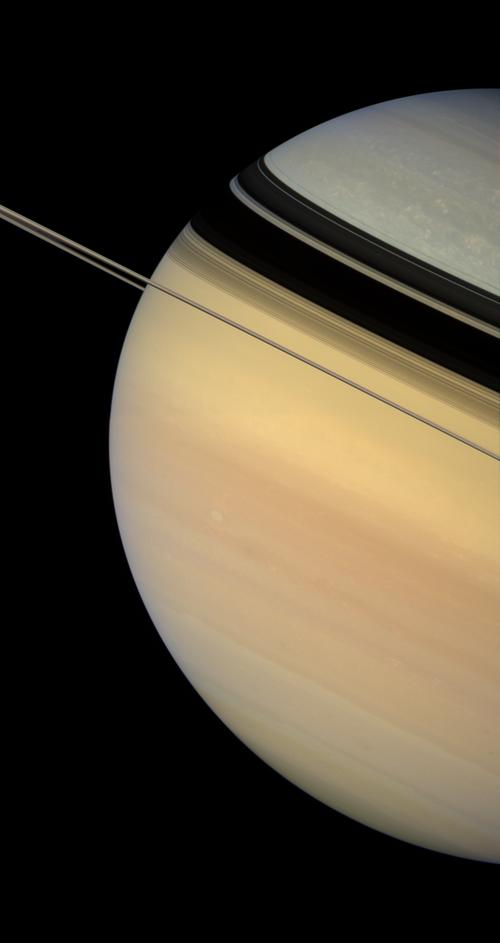
\includegraphics[max width=0.65\linewidth]{../images/saturn.jpg}\]

\begin{enumerate}
\def\labelenumi{\arabic{enumi})}
\tightlist
\item
  Cassini-Huyghens, ``Tourniquet shadows'',
  \texttt{http://saturn.jpl.nasa.gov/multimedia/images/image-details.cfm?imageID=2507}
\end{enumerate}

I learned some fun stuff about the foundations of quantum mechanics at
Les Treilles, so I want to mention that before I forget! I'll take a
little break from the Tale of Groupoidification\ldots{} though if you've
been following carefully, you may see it lurking beneath the surface.

Lately people have been developing ``foils for quantum mechanics'':
theories of physics that aren't classical, but aren't ordinary quantum
theory, either. These theories can lack some of the weird features of
quantum theory\ldots{} or, they may have ``supra-quantum'' features,
like the Popescu-Rohrlich box I mentioned last week.

The idea is not to take these theories seriously as models of our
universe --- though one can always dream. Instead, it's to explore the
logical possibilities, so we can see quantum mechanics and classical
mechanics as just two examples from a larger field of options, and
better understand what's special about them.

Rob Spekkens is a young guy who used to be at the Perimeter Institute;
now he's at DAMTP in Cambridge. At Les Treilles he gave a cool talk
about a simple theory that mimics some of features of quantum mechanics:

\begin{enumerate}
\def\labelenumi{\arabic{enumi})}
\setcounter{enumi}{1}
\tightlist
\item
  Rob Spekkens, ``Evidence for the epistemic view of quantum states: a
  toy theory'', \emph{Phys. Rev.~A} \textbf{75}, 032110 (2007). Also
  available as
  \href{https://arxiv.org/abs/quant-ph/0401052}{\texttt{quant-ph/0401052}}.
\end{enumerate}

The idea is to see how far you get using a very simple principle,
namely: even when you know as much as you can, there's an equal amount
you don't know.

In this setup, the complete description of a physical system involves
\(N\) bits of information, but you can only know \(N/2\) of them. When
you do an experiment to learn more information than that, the system's
state changes in a random way, so something you knew become obsolete.

The fraction ``\(1/2\)'' here is chosen for simplicity: it's just a toy
theory. But, it leads to some charming mathematical structures that I'd
like to understand better.

In this theory, the simplest nontrivial system is one whose state takes
two bits to describe --- but you can know at most one. Two bits of
information is enough to describe four states, say states \(1\), \(2\),
\(3\), and \(4\). But, since you can only know one bit of information,
you can't pin down the system's state completely. At most you can halve
the possibilities, and know something like ``the system is in state
\(1\) or \(3\)''. You can also be completely ignorant --- meaning you
only know ``the system is in state \(1\), \(2\), \(3\) or \(4\)''.

Since there are 3 ways to chop a \(4\)-element set in half, there are 3
``axes of knowledge'', namely

\begin{quote}
Is the system's state in \(\{1,2\}\) or \(\{3,4\}\)?\\
Is the system's state in \(\{1,3\}\) or \(\{2,4\}\)?\\
Is the system's state in \(\{1,4\}\) or \(\{2,3\}\)?
\end{quote}

You can only answer one of these questions.

This has a cute resemblance to how you can measure the angular momentum
of a spin-\(1/2\) particle along the \(x\), \(y\), or \(z\) axis, in
each case getting two choices. Spekkens has a nice picture in his paper:
\[
  \begin{tikzpicture}[scale=2.3]
    \node (c) at (0,0) {$\{1,2,3,4\}$};
    \node (r) at (1,0) {$\{2,3\}$};
    \node (t) at (0,1) {$\{1,2\}$};
    \node (l) at (-1,0) {$\{1,4\}$};
    \node (b) at (0,-1) {$\{3,4\}$};
    \node (tr) at (50:0.9) {$\{2,4\}$};
    \node (bl) at (230:0.9) {$\{1,3\}$};
    \draw[->] (l) to (c) to (r);
    \draw[->] (b) to (c) to (t);
    \draw[->] (bl) to (c) to (tr);
  \end{tikzpicture}
\] This octahedron is a discrete version of the ``Bloch ball''
describing mixed states of a spin-\(1/2\) particle in honest quantum
mechanics. If you don't know about that, I should remind you:

A ``pure state'' of a spin-\(1/2\) particle is a unit vector in
\(\mathbb{C}^2\), modulo phase. The set of these is just the Riemann
sphere!

In a pure state, we know as much as we can know. In a ``mixed state'',
we know less. Mathematically, a mixed state of a spin-\(1/2\) particle
is a \(2\times2\) ``density matrix'' --- a self-adjoint matrix with
nonnegative eigenvalues and trace \(1\). These form a \(3\)-dimensional
ball, the ``Bloch ball'', whose boundary is the Riemann sphere.

The \(x\), \(y\), and \(z\) coordinates of a point in the Bloch ball are
the expected values of the three components of angular momentum for a
spin-\(1/2\) particle in the given mixed state. The center of the Bloch
ball is the state of complete ignorance.

In honest quantum mechanics, the rotation group \(\mathrm{SO}(3)\) acts
as symmetries of the Bloch ball. In Spekken's toy version, this symmetry
group is reduced to the 24 permutations of the set \(\{1,2,3,4\}\). You
can think of these permutations as acting on a tetrahedron whose corners
are the 4 states of our system. The 6 corners of the octahedron above
are the midpoints of the edges of this tetrahedron!

Since Spekkens' toy system resembles a qubit, he calls it a ``toy bit''.
He goes on to study systems of several toy bits --- and the charming
combinatorial geometry I just described gets even more interesting.
Alas, I don't really understand it well: I feel there must be some
mathematically elegant way to describe it all, but I don't know what it
is.

Just as you can't duplicate a qubit in honest quantum mechanics --- the
famous \href{http://en.wikipedia.org/wiki/No_cloning_theorem}{no-cloning
theorem} --- it turns out you can't duplicate a toy bit. However,
\href{http://en.wikipedia.org/wiki/Bell's_theorem}{Bell's theorem} on
nonlocality and the
\href{http://plato.stanford.edu/entries/kochen-specker/}{Kochen-Specker
theorem} on contextuality don't apply to toy bits. Spekkens also lists
other similarities and differences.

All this is fascinating. It would be nice to find the mathematical
structure that underlies this toy theory, much as the category of
Hilbert spaces underlies honest quantum mechanics.

In my talk at Les Treilles, I explained how the seeming weirdness of
quantum mechanics arises from how the category of Hilbert spaces
resembles not the category of sets and functions, but a category with
``spaces'' as objects and ``spacetimes'' as morphism. This is good,
because we're trying to unify quantum mechanics with our best theory of
spacetime, namely general relativity. In fact, I think quantum mechanics
will make more sense when it's part of a theory of quantum gravity! To
see why, try this:

\begin{enumerate}
\def\labelenumi{\arabic{enumi})}
\setcounter{enumi}{2}
\tightlist
\item
  John Baez, ``Quantum quandaries: a category-theoretic perspective'',
  talk at Les Treilles, April 24, 2007,
  \texttt{http://math.ucr.edu/home/baez/treilles/}
\end{enumerate}

For more details, see my paper with the same title (see
\protect\hyperlink{week247}{``Week 247''}).

This fun paper by Bob Coecke gives another view of categories and
quantum mechanics, coming from work on quantum information theory:

\begin{enumerate}
\def\labelenumi{\arabic{enumi})}
\setcounter{enumi}{3}
\tightlist
\item
  Bob Coecke, ``Kindergarten quantum mechanics'', available as
  \href{https://arxiv.org/abs/quant-ph/0510032}{\texttt{quant-ph/0510032}}.
\end{enumerate}

To dig deeper, try these:

\begin{enumerate}
\def\labelenumi{\arabic{enumi})}
\setcounter{enumi}{4}
\item
  Samson Abramsky and Bob Coecke, ``A categorical semantics of quantum
  protocols'',
  \href{https://arxiv.org/abs/quant-ph/0402130}{\texttt{quant-ph/0402130}}.
\item
  Peter Selinger, ``Dagger compact closed categories and completely
  positive maps'', available at
  \texttt{http://www.mscs.dal.ca/\textasciitilde{}selinger/papers.html\#dagger}
\end{enumerate}

Since the category-theoretic viewpoint sheds new light on the no-cloning
theorem, Bell's theorem, quantum teleportation, and the like, maybe we
can use it to classify ``foils for quantum mechanics''. Where would
Spekkens' theory fit into this classification? I want to know!

Another mathematically interesting talk was by Howard Barnum, who works
at Los Alamos National Laboratory. Barnum works on a general approach to
physical theories using convex sets. The idea is that in any reasonable
theory, we can form a mixture or ``convex linear combination''
\[px + (1-p)y\] of mixed states \(x\) and \(y\), by putting the system
in state \(x\) with probability \(p\) and state \(y\) with probability
\(1-p\). So, mixed states should form a ``convex set''.

The Bloch sphere is a great example of such a convex set. Another
example is the octahedron in Spekken's theory. Another example is the
tetrahedron that describes the mixed states of a classical system with 4
pure states. Spekken's octahedron is a subset of this tetrahedron,
reflecting the limitations on knowledge in his setup.

To learn about the convex set approach, try these papers:

\begin{enumerate}
\def\labelenumi{\arabic{enumi})}
\setcounter{enumi}{6}
\item
  Howard Barnum, ``Quantum information processing, operational quantum
  logic, convexity, and the foundations of physics'', available as
  \href{https://arxiv.org/abs/quant-ph/0304159}{\texttt{quant-ph/0304159}}.
\item
  Jonathan Barrett, ``Information processing in generalized
  probabilistic theories'', available as
  \href{https://arxiv.org/abs/quant-ph/0508211}{\texttt{quant-ph/0508211}}.
\item
  Howard Barnum, Jonathan Barrett, Matthew Leifer and Alexander Wilce,
  ``Cloning and broadcasting in generic probabilistic theories'',
  available as
  \href{https://arxiv.org/abs/quant-ph/0611295}{\texttt{quant-ph/0611295}}.
\end{enumerate}

Actually I've been lying slightly: these papers also allow mixtures of
states \[px + qy\] where \(p+q\) is less than or equal to \(1\). For
example, if you prepare an electron in the ``up'' spin state with
probability \(p\) and the ``down'' state with probability \(q\), but
there's also a chance that you drop it on the floor and lose it, you
might want \(p+q < 1\).

I'm making it sound silly, but it's technically nice and maybe even
conceptually justified. Mathematically it means that instead of a convex
set of states, you have a vector space equipped with a convex cone and a
linear functional \(P\) such that the cone is spanned by the
``normalized'' states: those with \(P(x) = 1\). This is very natural in
both classical and quantum probability theory.

Quite generally, the normalized states form a convex set. Conversely,
starting from a convex set, you can create a vector space equipped with
a convex cone and a linear functional with the above properties.

So, I was only lying slightly. In fact, a complicated web of related
formalisms have been explored; you can learn about them from Barnum's
paper.

For example, the convex cone formalism seems related to the Jordan
algebra approach described in \protect\hyperlink{week162}{``Week 162''}.
Barnum cites a paper by Araki that shows how to get Jordan algebras from
sufficiently nice convex cones:

\begin{enumerate}
\def\labelenumi{\arabic{enumi})}
\setcounter{enumi}{9}
\tightlist
\item
  H. Araki, ``On a characterization of the state space of quantum
  mechanics'', \emph{Commun. Math. Phys.} \textbf{75} (1980), 1--24.
\end{enumerate}

It's a very interesting paper but a wee bit too technical for me to feel
like summarizing here.

Some nice examples of Jordan algebras are the \(2\times2\) self-adjoint
matrices with real, complex, quaternionic or octonionic entries. Each of
these algebras has a cone consisting of the nonnegative matrices, and
the trace gives a linear functional P. The nonnegative matrices with
trace = \(1\) are the mixed states of a spin-\(1/2\) particle in \(3\),
\(4\), \(6\), and \(10\)-dimensional spacetime, respectively! In each
case these mixed states form a convex set: a round ball generalizing the
Bloch ball. Similarly, the pure states form a sphere generalizing the
Riemann sphere.

Back in \protect\hyperlink{week162}{``Week 162''} I explained how these
examples are related to special relativity and spinors in different
dimensions. It's so cool I can't resist reminding you.

Our universe seems to like complex quantum mechanics. And, the space of
\(2\times2\) self-adjoint complex matrices --- let's call it
\(\mathrm{h}_2(\mathbb{C})\) --- is isomorphic to \(4\)-dimensional
Minkowski spacetime! The cone of positive matrices is isomorphic to the
future lightcone. The set of pure states of a spin-\(1/2\) particle is
the Riemann sphere \(\mathbb{CP}^1\), and this is isomorphic to the
``heavenly sphere'': the set of light rays through a point in Minkowski
spacetime.

This whole wonderful scenario works just as well in other dimensions if
we replace the complex numbers (\(\mathbb{C}\)) by the real numbers
(\(\mathbb{R}\)), the quaternions (\(\mathbb{H}\)) or the octonions
(\(\mathbb{O}\)):

\begin{itemize}
\tightlist
\item
  \(\mathrm{h}_2(\mathbb{R})\) is 3d Minkowski spacetime, and
  \(\mathbb{RP}^1\) is the heavenly sphere \(S^1\).
\item
  \(\mathrm{h}_2(\mathbb{C})\) is 4d Minkowski spacetime, and
  \(\mathbb{CP}^1\) is the heavenly sphere \(S^2\).
\item
  \(\mathrm{h}_2(\mathbb{H})\) is 6d Minkowski spacetime, and
  \(\mathbb{HP}^1\) is the heavenly sphere \(S^4\).
\item
  \(\mathrm{h}_2(\mathbb{O})\) is 10d Minkowski spacetime, and
  \(\mathbb{OP}^1\) is the heavenly sphere \(S^8\).
\end{itemize}

So, it's all very nice --- but a bit mysterious. Why did our universe
choose the complex numbers? We're told that scientists shouldn't ask
``why'' questions, but that's not really true --- the main thing is to
do it only to the extent that it leads to progress. But, sometimes you
just can't help it.

String theorists occasionally think about 10d physics using the
octonions, but not much. The strange thing about the octonions is that
the self-adjoint nxn octonionic matrices \(\mathrm{h}_n(\mathbb{O})\)
only form a Jordan algebra when \(n = 1\), \(2\), or \(3\). So, it seems
we can only describe very small systems in octonionic quantum mechanics!
Nobody knows what this means.

People working on the foundations of quantum mechanics have also thought
about real and quaternionic quantum mechanics.
\(\mathrm{h}_n(\mathbb{R})\), \(\mathrm{h}_n(\mathbb{C})\) and
\(\mathrm{h}_n(\mathbb{H})\) are Jordan algebras for all \(n\), so the
strange limitation afflicting the octonions doesn't affect these cases.
But, I wound up sharing a little cottage with Lucien Hardy at Les
Treilles, and he turns out to have thought about this issue. He pointed
out that something interesting happens when we try to combine two
quantum systems by tensoring them. The dimensions of
\(\mathrm{h}_n(\mathbb{C})\) behave quite nicely:
\[\dim(\mathrm{h}_{nm}(\mathbb{C})) = \dim(\mathrm{h}_n(\mathbb{C})) \dim(\mathrm{h}_m(\mathbb{C}))\]
But, for the real numbers we usually have
\[\dim(\mathrm{h}_{nm}(\mathbb{R})) > \dim(\mathrm{h}_n(\mathbb{R})) \dim(\mathrm{h}_m(\mathbb{R}))\]
and for the quaternions we usually have
\[\dim(\mathrm{h}_{nm}(\mathbb{H})) < \dim(\mathrm{h}_n(\mathbb{H})) \dim(\mathrm{h}_m(\mathbb{H}))\]
So, it seems that when we combine two systems in real quantum mechanics,
they sprout mysterious new degrees of freedom! More precisely, we can't
get all density matrices for the combined system as linear combinations
of tensor products of density matrices for the two systems we combined.
For the quaternions the opposite effect happens: the combined system has
fewer mixed states than we'd expect.

This observation lurks behind axiom 4 in this paper:

\begin{enumerate}
\def\labelenumi{\arabic{enumi})}
\setcounter{enumi}{10}
\tightlist
\item
  Lucien Hardy, ``Quantum theory from five reasonable axioms'',
  available as
  \href{https://arxiv.org/abs/quant-ph/0101012}{\texttt{quant-ph/0101012}}.
\end{enumerate}

Another special way in which \(\mathbb{C}\) is better than
\(\mathbb{H}\) or \(\mathbb{R}\) is that only for a complex Hilbert
space is there a correspondence between continuous \(1\)-parameter
groups of unitary operators and self-adjoint operators. We always get a
\emph{skew-adjoint} operator, but only in the complex case can we
convert this into a self-adjoint operator by dividing by \(i\).

Here are some more references, kindly provided by Rob Spekkens. The
pioneering quantum field theorist Stückelberg wrote a bunch of papers on
real quantum mechanics. Spekkens recommends this one:

\begin{enumerate}
\def\labelenumi{\arabic{enumi})}
\setcounter{enumi}{11}
\tightlist
\item
  E. C. G. Stückelberg, ``Quantum theory in real Hilbert space'',
  \emph{Helv. Phys. Acta} \textbf{33}, 727 (1960).
\end{enumerate}

This is a modern review:

\begin{enumerate}
\def\labelenumi{\arabic{enumi})}
\setcounter{enumi}{12}
\tightlist
\item
  Jan Myrheim, ``Quantum mechanics on a real Hilbert space'', available
  \href{https://arxiv.org/abs/quant-ph/9905037}{\texttt{quant-ph/9905037}}.
\end{enumerate}

What I find most fascinating is the connection between real quantum
mechanics and time reversal symmetry. In ordinary complex quantum
mechanics, time reversal symmetry is sometimes described by a
conjugate-linear (indeed ``antiunitary'') operator \(T\) with
\(T^2 = 1\). Such an operator is precisely a ``real structure'' on our
complex Hilbert space: it picks out a real Hilbert subspace of which our
complex Hilbert space is the complexification.

It's worth adding that in the physics of fermions, another possibility
occurs: an antiunitary time reversal operator with \(T^2 = -1\). This is
precisely a ``quaternionic structure'' on our complex Hilbert space: it
makes it into a quaternionic Hilbert space!

For more on these ideas try:

\begin{enumerate}
\def\labelenumi{\arabic{enumi})}
\setcounter{enumi}{13}
\item
  Freeman J. Dyson, ``The threefold way: algebraic structure of symmetry
  groups and ensembles in quantum mechanics'', \emph{Jour. Math. Phys.}
  \textbf{3} (1962), 1199--1215.
\item
  John Baez, ``Symplectic, quaternionic, fermionic'',
  \texttt{http://math.ucr.edu/home/baez/symplectic.html}
\end{enumerate}

From all this one can't help but think that complex, real, and
quaternionic quantum mechanics fit together in a unified structure, with
the complex numbers being the most important, but other two showing up
naturally in systems with time reversal symmetry.

Stephen Adler --- famous for the Adler-Bell-Jackiw anomaly --- spent a
long time at the Institute for Advanced Studies working on quaternionic
quantum mechanics:

\begin{enumerate}
\def\labelenumi{\arabic{enumi})}
\setcounter{enumi}{15}
\tightlist
\item
  S. L. Adler, \emph{Quaternionic Quantum Mechanics and Quantum Fields},
  Oxford U. Press, Oxford, 1995.
\end{enumerate}

A problem with this book is that it defines a quaternionic vector space
to be a \emph{left} module of the quaternions, instead of a
\emph{bimodule}. This means you can't naturally tensor two quaternionic
vector spaces and get a quaternionic vector space! Adler ``solves'' this
problem by noting that any left module of the quaternions becomes a
right module, and in fact a bimodule, via \[xq = q^*x\] But, when you're
working with a noncommutative ring, you really need to think about left
modules, right modules, and bimodules to understand the theory of tensor
products. And, the quaternions have more bimodules than you might
expect: for example, for any automorphism of the quaternions:
\[f\colon H \to H\] there's a way to make \(H\) into an \(H\)-bimodule
with the obvious left action and a ``twisted'' right action, where \(q\)
acts on \(x\) to give \[x f(q)\] Since the automorphism group of the
quaternions is \(\mathrm{SO}(3)\), there turn out to be
\(\mathrm{SO}(3)\)'s worth of nonisomorphic ways to make \(H\) into an
\(H\)-bimodule!

For an attempt to tackle this issue, see:

\begin{enumerate}
\def\labelenumi{\arabic{enumi})}
\setcounter{enumi}{16}
\tightlist
\item
  John Baez and Toby Bartels, ``Functional analysis with quaternions'',
  available at \texttt{http://toby.bartels.name/papers/\#quaternions}
\end{enumerate}

However, it's possible we'll only see what real and quaternionic quantum
mechanics are good for when we work in the \(3\)-category
\(\mathsf{Alg}(\mathbb{R})\) mentioned in
\protect\hyperlink{week209}{``Week 209''}, taking \(\mathbb{R}\) to be
the real numbers. Here:

\begin{itemize}
\tightlist
\item
  there's one object, the real numbers \(\mathbb{R}\).
\item
  the \(1\)-morphisms are algebras \(A\) over \(\mathbb{R}\).
\item
  the \(2\)-morphisms \(M\colon A \to B\) are \((A,B)\)-bimodules.
\item
  the \(3\)-morphisms \(f\colon M \to N\) are \((A,B)\)-bimodule
  morphisms.
\end{itemize}

This could let us treat real, complex and quaternionic quantum mechanics
as part of a single structure.

Dreams, dreams\ldots.

\begin{center}\rule{0.5\linewidth}{0.5pt}\end{center}

\textbf{Addenda:} In email, Scott Aaronson pointed out this nice
webpage:

\begin{enumerate}
\def\labelenumi{\arabic{enumi})}
\setcounter{enumi}{17}
\tightlist
\item
  Scott Aaronson, ``Lecture 9: Quantum'',
  \texttt{http://www.scottaaronson.com/democritus/lec9.html}
\end{enumerate}

He wrote:

\begin{quote}
I talk all about the known differences between QM over the complex
numbers and QM over the reals and quaternions (including the
parameter-counting difference you mentioned, but also a couple you
didn't), and why the universe might've gone with complex numbers.
\end{quote}

His lecture also cites this paper:

\begin{enumerate}
\def\labelenumi{\arabic{enumi})}
\setcounter{enumi}{18}
\tightlist
\item
  Carlton M. Caves, Christopher A. Fuchs, and Ruediger Schack, ``Unknown
  quantum states: the quantum de Finetti representation'', available as
  \href{http://www.arxiv.org/abs/quant-ph/0104088}{\texttt{quant-ph/0104088}}.
\end{enumerate}

which Rob Spekkens also pointed out to me.

The quantum de Finetti theorem is a generalization of the
\href{http://en.wikipedia.org/wiki/De_Finetti's_theorem}{classical de
Finetti theorem}. Both classical quantum de Finetti theorems are about
\(n\) copies of a system sitting side by side in an ``exchangeable''
state: a state that's not only invariant under permutations of the
copies, but lacking correlations between the different copies!

Here's the quantum de Finetti theorem. Suppose you have an
``exchangeable'' density operator \(\rho_n\) on \(H^{\otimes n}\) ---
that is, one such that for each \(N \geqslant n\), there's a density
operator \(\rho_N\) on \(H^{\otimes N}\) which 1) is invariant under
permutations in \(S_N\) and 2) has \(\rho\) as its marginal, meaning
that \[\mathrm{Tr}(\rho_N) = \rho_n\] where \(\mathrm{Tr}\) is the
partial trace map sending operators on \(H^{\otimes N}\) to operators on
\(H^{\otimes n}\). Then, \(\rho_n\) is a mixture of density matrices of
the form \(\rho \otimes \ldots \otimes \rho\): a tensor product of \(n\)
copies of a density matrix on \(H\).

This is completely plausible if you know what all this jargon means.

And now for the punch line: \emph{This theorem would \textbf{fail} if we
did quantum mechanics using the real numbers!}

Of course, this is related to the fact I mentioned this Week, namely
that for real quantum mechanics, ``the whole is more than the product of
its parts'' in a more severe way than for complex quantum mechanics.

Bob Coecke wrote:

\begin{quote}
The standard references on quaternionic QM are:

\begin{enumerate}
\def\labelenumi{\arabic{enumi})}
\setcounter{enumi}{19}
\item
  D. Finkelstein, J.M. Jauch, S. Schiminovich and D. Speiser,
  ``Foundations of quaternion quantum mechanics'', \emph{Journal of
  Mathematical Physics} \textbf{3}, 207 (1962).
\item
  D. Finkelstein, J.M. Jauch, S. Schiminovich and D. Speiser, ``Some
  physical consequences of general Q-covariance'', \emph{Helvetica
  Physica Acta} \textbf{35}, 328--329 (1962).
\item
  D. Finkelstein, J.M. Jauch, S. Schiminovich and D. Speiser,
  ``Principle of general Q-covariance'', \emph{Journal of Mathematical
  Physics} \textbf{4}, 788--796 (1963).
\end{enumerate}

A standard structural result in the order-theoretic vein which separates
Reals, Complex Numbers and Quaternions from ``non-classical fields'' is:

\begin{enumerate}
\def\labelenumi{\arabic{enumi})}
\setcounter{enumi}{22}
\tightlist
\item
  M. P. Soler (1995) ``Characterization of Hilbert spaces with
  orthomodular spaces'', \emph{Comm. Algebra} \textbf{23}, pp.~219--243.
\end{enumerate}

It does this relative to the order-theoretic characterization of Hilbert
spaces:

\begin{enumerate}
\def\labelenumi{\arabic{enumi})}
\setcounter{enumi}{23}
\item
  C. Piron (1964, French) ``Axiomatique Quantique'', \emph{Helv. Phys.
  Acta} \textbf{37}, pp.~439--468.
\item
  I. Amemiya and H. Araki (1966) ``A Remark on Piron's Paper'',
  \emph{Publ. Res. Inst. Math. Sci. Ser. A} \textbf{2}, pp.~423--427.
\item
  C. Piron (1976) \emph{Foundations of Quantum Physics}, W. A. Benjamin,
  Inc., Reading.
\end{enumerate}

A nicely written recent survey on this stuff is:

\begin{enumerate}
\def\labelenumi{\arabic{enumi})}
\setcounter{enumi}{25}
\tightlist
\item
  Isar Stubbe and B. van Steirteghem (2007) ``Propositional systems,
  Hilbert lattices and generalized Hilbert spaces'', chapter in:
  \emph{Handbook Quantum Logic} (edited by D. Gabbay, D. Lehmann and K.
  Engesser), Elsevier, to appear. Available at
  \texttt{http://www.win.ua.ac.be/\textasciitilde{}istubbe/}
\end{enumerate}

It is not clear to me how exactly this order-theoretic stuff relates to
the \emph{thick} categorical axiomatics for QM John mentioned above. One
key difference is that in the order-theoretic axiomatics one failed to
find an abstract counterpart to the Hilbert space tensor product. (ie
without having to say that we are working in the lattice of closed
subspaces of a Hilbert space) On the other hand, the categorical
approach starting from symmetric monoidal categories takes that
description of compound systems as an a priori. Singling out the complex
numbers is done in terms of two involutions on morphisms, one covariant
and one contravariant, where the covariant one capture complex
conjugation ie the unique non-trivial automorphism characteristic of
complex numbers. The contravariant one captures transposition and
together they make up the adjoint.
\end{quote}

Here ``thick'' refers to working with categories which nice big
hom-sets, instead of mere posets or preorders, which are categories with
at most one morphism from one object to another.

Rob Spekkens also gives some references on quantum computation in real
quantum mechanics. He writes:

\begin{quote}
See also:

\begin{enumerate}
\def\labelenumi{\arabic{enumi})}
\setcounter{enumi}{26}
\tightlist
\item
  C. M. Caves, C. A. Fuchs, P. Rungta, ``Entanglement of formation of an
  arbitrary state of two rebits'', available as
  \href{http://arxiv.org/abs/quant-ph/0009063}{\texttt{quant-ph/0009063}}.
\end{enumerate}

It's also worth noting that quantum computation and quantum cryptography
do not require the complex field. Have a look at:

\begin{enumerate}
\def\labelenumi{\arabic{enumi})}
\setcounter{enumi}{27}
\tightlist
\item
  T. Rudolph and L. Grover, ``A 2 rebit gate universal for quantum
  computing'',
  \href{http://arxiv.org/abs/quant-ph/0210187}{\texttt{quant-ph/0210187}}.
\end{enumerate}

I actually know of no information-theoretic task whose possibility is
contingent on the nature of the number field.
\end{quote}

More discussion (and pictures!) can be found at the
\href{http://golem.ph.utexas.edu/category/2007/05/this_weeks_finds_in_mathematic_12.html}{\(n\)-Category
Café}.



\hypertarget{week252}{%
\section{May 27, 2007}\label{week252}}

Today I want to tell you about the electromagnetic snake at the center
of our Galaxy, and continue the Tale of Groupoidification.

But first, the long-range weather forecast. There's a 40\% chance of
rain on Neptune in 8 billion years! More precisely, that's the chance
these authors give for the formation of an ocean on Neptune when its
interior cools down enough:

\begin{enumerate}
\def\labelenumi{\arabic{enumi})}
\tightlist
\item
  Sloane J. Wiktorowica and Andrew P. Ingersoll, ``Liquid water oceans
  in ice giants'', available as
  \href{https://arxiv.org/abs/astro-ph/0609723}{\texttt{astro-ph/0609723}}.
\end{enumerate}

Right now, even though Neptune is named after the Roman god of seas and
has a nice blue appearance:
\[\href{http://en.wikipedia.org/wiki/Neptune}{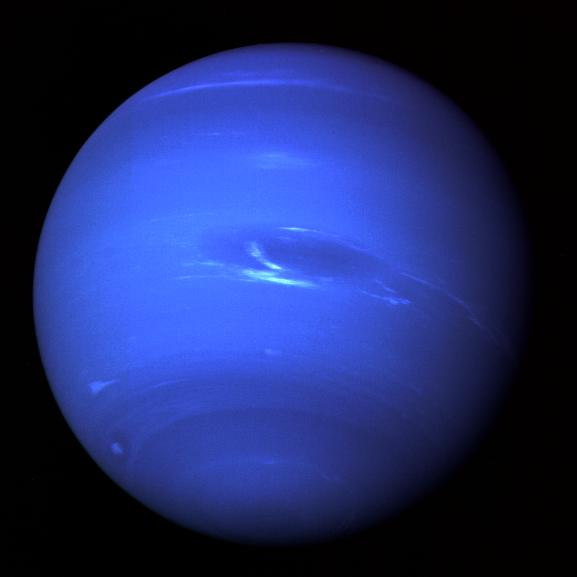
\includegraphics[max width=0.65\linewidth]{../images/neptune.jpg}}\]
it's mighty dry --- at least on top. Spectroscopy detects no water at
all in its upper atmosphere! But that's consistent with the presence of
water down below, since water vapor is a lot heavier than hydrogen and
helium, which make up most of Neptune's upper atmosphere, and the pull
of gravity there is mighty fierce.

In fact, scientists believe Neptune has a core of molten metal and rock
surrounded by more rock, methane ice, ammonia ice, and water ice --- all
solid due to high pressures. The overall density of Neptune makes sense
if there's a lot of water down there. But, Wiktorowica and Ingersoll
argue that the planet can't have an ocean of liquid water.

Surprisingly, this is because Neptune is too \emph{hot} --- even though
its upper atmosphere is a chilly 50 kelvin! I think their argument goes
roughly like this, though I don't understand it well. If you fell down
through the atmosphere of Neptune, you'd find that it gets hotter and
hotter as you go down, and moister and moister too --- but always too
hot, given the amount of moisture, for liquid water to be more stable
than water vapor.

However, they also indulge in some predictions about the far future!

First let's set the stage:

\begin{itemize}
\tightlist
\item
  In 1.1 billion years the Sun will become 10\% brighter than now, and
  the Earth's atmosphere will dry out.
\item
  In 3 billion years the Andromeda Galaxy will collide with our galaxy.
  Many solar systems will be destroyed.
\item
  In 3.5 billion years the Sun will become 40\% brighter than today. If
  the Earth is still orbiting the sun, its oceans will evaporate.
\item
  In 5.4 billion years from now the Sun's core will run out of hydrogen.
  It will enter its first red giant phase, becoming 1.6 times bigger and
  2.2 times brighter than today.
\item
  In 6.5 billion years from now the Sun will become a full-fledged red
  giant, 170 times bigger and 2400 times brighter than today. The
  Republican Party will finally admit the existence of global warming,
  but point out that it's not human-caused.
\item
  In 6.7 billion years from now the Sun will start fusing helium and
  shrink back down to 10 times bigger and 40 times brighter than today.
\item
  In 6.8 billion years from now the Sun will run out of helium. Being
  too small to start fusing carbon and oxygen, it'll enter a second red
  giant phase, growing 180 times bigger and 3000 times brighter than
  today.
\end{itemize}

But then, about 6.9 billion years from now, the Sun will start
pulsating, ejecting half of its mass in the form of solar wind! It'll
become what they call a ``planetary nebula''. Eventually only its inner
core will be left. In \protect\hyperlink{week223}{``Week 223''} I quoted
Bruce Balick's eloquent description:

\begin{quote}
The remnant Sun will rise as a dot of intense light, no larger than
Venus, more brilliant than 100 present Suns, and an intensely hot
blue-white color hotter than any welder's torch. Light from the fiendish
blue ``pinprick'' will braise the Earth and tear apart its surface
molecules and atoms. A new but very thin ``atmosphere'' of free
electrons will form as the Earth's surface turns to dust.
\end{quote}

This is where Wiktorovika and Ingersoll \emph{begin} their story. So
far, Neptune will have warmed up a lot --- assuming for the sake of
argument that it wasn't thrown out of the Solar System when the Milky
Way hit Andromeda. But when the Sun loses mass, Neptune will either
collide with Uranus, be ejected from the Solar System, or assume a
stable orbit about twice its current size.

In the latter two scenarios, Neptune will chill out, at least when the
remnant Sun cools down and becomes a white dwarf. When the surface
temperature of Neptune reaches 30 kelvin, they estimate it has a 41.5\%
plus or minus 4.2\% chance of forming oceans.

So, they say: ``Billions of years from now, after the Sun has gone,
Neptune may therefore become the only object in the Solar system with
liquid water oceans''.

This sounds nice --- but don't buy your beachfront property there yet.

First, they don't study how the atmospheric composition of Neptune may
change when the Sun gets 3000 times brighter than now! Maybe this will
\emph{help} Neptune form oceans. After all, light gases like molecular
hydrogen and helium, which dominate Neptune's upper atmosphere now, are
more likely than water vapor to be driven off into outer space when it
gets hot. But, they don't even check to see if Neptune will have
\emph{any} atmosphere left after this era.

Second, the estimate of a ``41.5\% plus or minus 4.2\% chance'' seems
strangely precise, given the uncertainties involved. The error bars
should probably have big error bars themselves!

Third, it's worth admitting that the atmosphere of Neptune is a bit
mysterious. For example, nobody knows why it's bright blue. It's
probably because of methane --- but Uranus also has methane in its
atmosphere, and it's not as blue:
\[\href{http://en.wikipedia.org/wiki/Uranus}{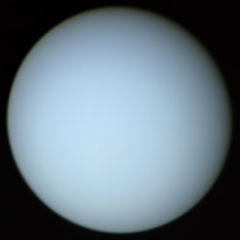
\includegraphics[max width=0.65\linewidth]{../images/uranus.jpg}}\]
Also, despite being the coldest planet in our Solar System, Neptune has
the fastest winds: up to 2100 kilometers per hour, almost supersonic!
Nobody knows what powers these winds.

When the Voyager 2 spacecraft flew by Neptune in 1992, it saw a storm
system the size of Eurasia, which was dubbed ``The Great Dark Spot'':
\[\href{http://en.wikipedia.org/wiki/Great_Dark_Spot}{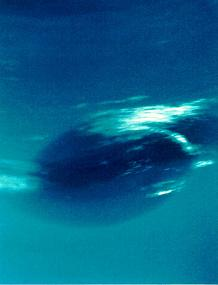
\includegraphics[max width=0.65\linewidth]{../images/neptune_great_dark_spot.jpg}}\]
It seemed to resemble the Great Red Spot on Jupiter, which has been
around for at least 177 years. But when the Hubble Space Telescope took
another good look at Neptune in 1994, the Great Dark Spot was gone!
Meanwhile, other storms had formed.

So, the weather on Neptune is dynamic and poorly understood. Doing
forecasts for the next 8 billion years seems pretty risky\ldots{} though
fun.

Of course, liquid water oceans are nice if you're looking for life. And
while there probably isn't life on Neptune, there could be life on
similar planets in other solar systems. So far people have found 233 of
these ``exoplanets'', most of them heavier than Jupiter but close to
their suns --- because such planets are the easiest to detect by how
they pull on their sun.

Here's a chart showing the masses and orbital radii of known exoplanets
as of 2004:
\[\href{http://en.wikipedia.org/wiki/Extrasolar_planet}{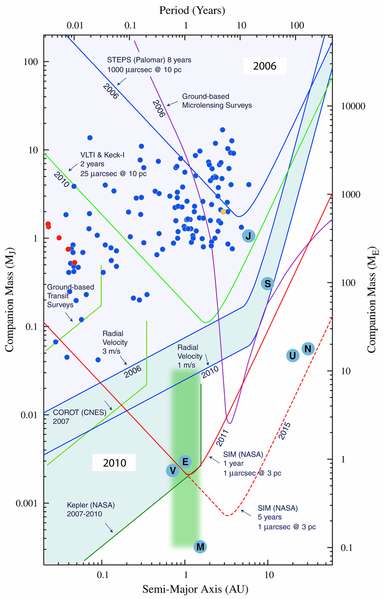
\includegraphics[max width=0.65\linewidth]{../images/exoplanets.png}}\]

\begin{enumerate}
\def\labelenumi{\arabic{enumi})}
\setcounter{enumi}{1}
\tightlist
\item
  P. R. Lawson, S. C. Unwin, and C. A. Beichman, ``Precursor Science for
  the Terrestrial Planet Finder'', \emph{JPL Pub} \textbf{04-014},
  Oct.~2004, page 21, fig.~5. Chart at
  \texttt{http://en.wikipedia.org/wiki/Image:Extrasolar\_Planets\_2004-08-31.png}.
  Report at
  \texttt{http://planetquest.jpl.nasa.gov/documents/RdMp272.pdf}
\end{enumerate}

For comparison, the letters V, E, M, J, S, U, N, stand for planets in
our Solar System, not counting Mercury or the subsequently dethroned
Pluto.

As you'll see, there are lots of ``hot Jupiters'' --- planets as big as
Jupiter, or even up to 200 times heavier, but closer to their sun than
we are to ours. Recently a postdoc at UCLA found evidence for water in
the atmosphere of one of these planets:

\begin{enumerate}
\def\labelenumi{\arabic{enumi})}
\setcounter{enumi}{2}
\tightlist
\item
  Travis Barman, ``Identification of absorption features in an
  extrasolar planet atmosphere'', available as
  \href{http://www.arxiv.org/abs/0704.1114}{\texttt{arxiv:0704.1114}}.
\end{enumerate}

This planet is only 7 million kilometers away from its yellow-white Sun,
much closer than Mercury is to ours. Its year is only 3.5 of our days!
It's bigger in size than Jupiter, but only 0.7 times as heavy. Its
surface temperature must be about 1000 kelvin. That's one really hot
Jupiter.

People have also been finding ``hot Neptunes''. In fact, I read about a
nice one in the newspaper while writing this! It's called Gliese 436 b.
It's the size of Neptune and it's orbiting the red dwarf star Gliese
436, which is 33 light-years from Earth. This star is only 1\% as bright
as our Sun --- but the planet is so close that its year lasts less than
three of our days! So, its surface temperature is high: higher than the
melting point of lead.

However, because this planet is so big, the pressure down below can
still make water into a solid. In fact, its density suggests that it's
mainly made of ice!

I think this is the paper that triggered the newspaper reports:

\begin{enumerate}
\def\labelenumi{\arabic{enumi})}
\setcounter{enumi}{3}
\tightlist
\item
  M. Gillon et al, ``Detection of transits of the nearby hot Neptune GJ
  436 b'', available as
  \href{http://www.arxiv.org/abs/0705.2219}{\texttt{arxiv:0705.2219}}.
\end{enumerate}

It seems hot Neptunes like this could have started as hot Jupiters and
then lost a lot of their atmosphere:

\begin{enumerate}
\def\labelenumi{\arabic{enumi})}
\setcounter{enumi}{4}
\tightlist
\item
  I. Baraffe, G. Chabrier, T. S. Barman, F. Selsis, F. Allard, and P. H.
  Hauschildt, ``Hot-Jupiters and hot-Neptunes, a common origin?'',
  available at
  \href{http://www.arxiv.org/abs/astro-ph/0505054}{\texttt{astro-ph/0505054}}.
\end{enumerate}

There could also be cold Neptunes, perhaps with liquid water oceans. We
haven't seen these yet, but they'd be hard to see. So, while Wiktorowica
and Ingersoll's paper doesn't convince me about the future of \emph{our}
Neptune, it raises some interesting possibilities.

Next: the snake at the center of our galaxy!

Gregory Benford is best known for his science fiction, which spans the
galaxy, but he's also an astrophysicist at U. C. Irvine. Recently he
spent a week at my school, U. C. Riverside, which has one of the world's
best SF libraries: the \href{http://eaton-collection.ucr.edu/}{Eaton
Collection}. Since my wife is involved in the SF program at the
comparative literature department here, he had dinner at our place one
night. The conversation drifted all over the place, with a heavy focus
on fruit flies that have been bred to live twice as long as usual. But
when I asked him about his research, he said he'd written some papers
about enormous glowing filaments near the center of the Milky Way.

I hadn't known about these! He said the biggest one could be a million
years old, perhaps formed by some energetic event, maybe a star falling
into the central black hole. Here's an expository paper he wrote about
it:

\begin{enumerate}
\def\labelenumi{\arabic{enumi})}
\setcounter{enumi}{5}
\tightlist
\item
  Gregory Benford, ``The electromagnetic snake at the galactic center'',
  \texttt{http://www.ps.uci.edu/physics/news3/benford.html}
\end{enumerate}

I'll just quote a little:

\begin{quote}
Five years ago radio astronomy revealed the oddest and longest filament
yet discovered at our galactic center: a uniquely kinked structure about
150 light years long and two to three light years wide --- the Snake.
Its large kinks are its brightest parts. There is energetic activity at
one end and a supernova bubble at the other, which the Snake appears to
penetrate unharmed.

How does nature form stable, long-lived magnetic structures which
display considerable polarization (about 60\% at 10.55 GHz in the
Snake)? In 1988 I had modeled others of the dozens of filaments seen
uniquely at the galactic center in terms of an electrodynamic view, in
which currents set up coherent magnetic pinches. Such self-organizing
filaments can exist in laboratory plasmas for long times; the galactic
ones could be at least a million years old, as estimated by the time
that shear forces would disrupt them.

The electrodynamic view uses pinch forces of currents to form filaments,
driven by the \(E = v \times B\) of conducting molecular clouds moving
across a strong milliGauss ambient, ordered field. A return current must
then flow at larger radii, making a closed loop which has a springy
flexibility, able to withstand the turbulent velocity fields known near
the galactic center. The picture then anticipates that aberrant
molecular clouds, moving contrary to the general galactic rotation,
should accompany each filament. This prediction has held up as more
filaments were found.
\end{quote}

I'd like to learn more about these!

Back in \protect\hyperlink{week248}{``Week 248''}, I mentioned some of
the complex things that electromagnetic fields and plasma do in the Sun.
The center of the Galaxy is another place where
electromagnetohydrodynamics runs rampant. There's a black hole there, of
course, but also these filaments, and a fairly strong magnetic field
that contains about \(4\times10^{47}\) joules of energy within about 300
light years of the galactic center. By comparison, a supernova emits a
mere \(10^{44}\) joules. So, there's a lot of energy around\ldots.

The big picture here, created by Farhad Yusef-Zadeh and collaborators,
shows the galactic center quite nicely, as viewed in radio frequencies:
\[\href{http://www.nrao.edu/pr/2004/filaments/}{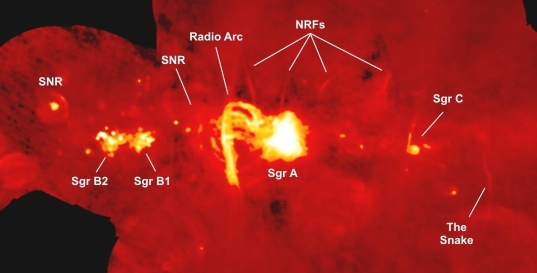
\includegraphics[max width=0.65\linewidth]{../images/galactic_center.jpg}}\]

\begin{enumerate}
\def\labelenumi{\arabic{enumi})}
\setcounter{enumi}{6}
\tightlist
\item
  National Radio Astronomy Observatory, ``Origin of enigmatic
  galactic-center filaments revealed'',
  \texttt{http://www.nrao.edu/pr/2004/filaments/}
\end{enumerate}

You can see some supernova remnants (SNRs), the region Sgr A which
contains the black hole at the galactic center, various nonthermal radio
filaments (NRFs), and the Snake. Some of these filaments come from
regions where stars are forming\ldots{} that could be important.

But, this article discusses another piece of the puzzle --- the possible
role of turbulence in winding up the galactic magnetic field:

\begin{enumerate}
\def\labelenumi{\arabic{enumi})}
\setcounter{enumi}{7}
\tightlist
\item
  Stanislav Boldyrev and Farhad Yusef-Zadeh, ``Turbulent origin of the
  galactic-center magnetic field: nonthermal radio filaments'',
  available as
  \href{https://arxiv.org/abs/astro-ph/0512373}{\texttt{astro-ph/0512373}}.
\end{enumerate}

It's a complicated stew. I don't hope to understand it, just admire it.

And finally: the Tale of Groupoidification! In
\protect\hyperlink{week250}{``Week 250''} we reached the point of seeing
how spans of groupoids over a fixed group \(G\) subsume the theory of
\(G\)-sets and invariant relations between these --- which are
traditionally studied using ``double cosets''.

There is a lot more we could say about this. But, our most urgent goal
is to see how spans of groupoids act like twice categorified matrices
--- matrices whose entries are not just \emph{numbers}, and not just
\emph{sets}, but \emph{groupoids}! This will expose the secret
combinatorial underpinnings of a lot of fancy linear algebra. Once we've
categorified linear algebra this way, we'll be in a great position to
tackle fashionable topics like categorified quantum groups, invariants
of higher-dimensional knots, and the like.

But, we should restrain ourselves from charging ahead too fast!
Everything will hang together better if we lay the groundwork properly.
For this, it pays to re-examine the history of mathematics a bit. If
we're trying to understand linear algebra using groupoids, it pays to
ask: how did people connect linear algebra and group theory in the first
place?

This book is very helpful:

\begin{enumerate}
\def\labelenumi{\arabic{enumi})}
\setcounter{enumi}{8}
\tightlist
\item
  Charles W. Curtis, \emph{Pioneers of Representation Theory: Frobenius,
  Burnside, Schur and Brauer}, History of Mathematics vol.~\textbf{15},
  AMS, Providence, Rhode Island, 1999.
\end{enumerate}

Back in 1897, a mathematician named William Burnside wrote the first
book in English on finite groups. It was called Theory of Groups of
Finite Order.
\[\href{http://www-groups.dcs.st-and.ac.uk/~history/Biographies/Burnside.html}{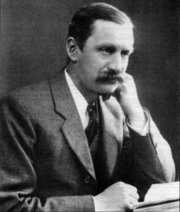
\includegraphics[max width=0.65\linewidth]{../images/burnside.jpg}}\]
In the preface, Burnside explained why he studied finite groups by
letting them act as permutations of sets, but not as linear
transformations of vector spaces:

\begin{quote}
Cayley's dictum that ``a group is defined by means of the laws of
combination of its symbols'' would imply that, in dealing with the
theory of groups, no more concrete mode of representation should be used
than is absolutely necessary. It may then be asked why, in a book that
professes to leave all applications to one side, a considerable space is
devoted to substitution groups {[}permutation groups{]}, but other
particular modes of representation, such as groups of linear
transformations, are not even referred to. My answer to this question is
that while, in the present state of our knowledge, many results in the
pure theory are arrived at most readily by dealing with properties of
substitution groups, it would be difficult to find a result that could
most directly be obtained by the consideration of groups of linear
transformations.
\end{quote}

In short, he didn't see the point of representing groups on vector
spaces --- at least as a tool in the ``pure'' theory of finite groups,
as opposed to their applications.

However, within months after this book was published, he discovered the
work of Georg Frobenius, who used linear algebra very effectively to
study groups!
\[\href{http://www-groups.dcs.st-and.ac.uk/~history/Biographies/Frobenius.html}{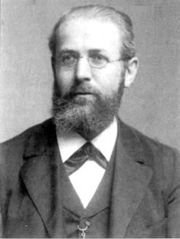
\includegraphics[max width=0.65\linewidth]{../images/frobenius.jpg}}\]
So, Burnside started using linear algebra in his own work on finite
groups, and by the time he wrote the second edition of his book in 1911,
he'd changed his tune completely:

\begin{quote}
Very considerable advances in the theory of groups of finite order have
been made since the appearance of the first edition of this book. In
particular the theory of groups of linear substitutions has been the
subject of numerous and important investigations by several writers; and
the reason given in the original preface for omitting any account of it
no longer holds good. In fact it is now more true to say that for
further advances in the abstract theory one must look largely to the
representation of a group as a group of linear transformations.
\end{quote}

It's interesting to see exactly how representing finite groups on vector
spaces lets us understand them better. By now almost everyone agrees
this is true. But how much of the detailed machinery of linear algebra
is really needed? How much we could do purely combinatorially, using
just spans of groupoids?

I don't really know the full answer to this question. But, it quickly
leads us into the fascinating theory of ``Hecke operators'', which will
play a big role in the Tale of Groupoidification. So, let's pursue it a
bit.

Suppose we have two guys, William and Georg, who are studying a finite
group \(G\).

William says, ``I'm studying how \(G\) acts on sets.''

Georg replies, ``I'm studying how it acts on complex vector spaces, as
linear transformations. Mere sets are feeble entities. I can do anything
you can do --- but I have the tools of linear algebra to help me!''

William says, ``But, you're paying a moral price. You're getting the
complex numbers --- a complicated infinite thing --- involved in what
should be a completely finitary and combinatorial subject: the study of
a finite group. Is this really necessary?''

Georg replies, ``I don't know, but it's sure nice. For example, suppose
I have \(G\) acting on vector space \(V\). Then I can always break down
\(V\) into a direct sum of subspaces preserved by \(G\), which can't
themselves be broken down any further. In technical terms: every
representation of \(G\) is a direct sum of irreducible representations.
And, this decomposition is unique! It's very nice: it's a lot like how
every natural integer has a unique prime factorization.''

William says, ``Yes, it's always fun when we can break things down into
`atoms' that can't be further decomposed. It's very satisfying to our
reductionist instincts. But, I can do even better than you!''

Georg raises an eyebrow. ``Oh?''

``Yeah,'' William says. ``Suppose I have our group \(G\) acting on a set
\(S\). Then I can always break down \(S\) into a disjoint union of
subsets preserved by \(G\), which can't themselves be broken down any
further. In technical terms: every action of \(G\) is a disjoint union
of transitive actions. And, this decomposition is unique!''

Embarrassed, Georg replies, ``Oh, right --- we heard that back in
\protect\hyperlink{week249}{"Week 249"}. I wasn't paying enough
attention. But how is what you're doing better than what I'm doing? It
sounds just the same.''

William hesitates. "Well, first of all, a rather minor point, which I
can't resist mentioning \ldots{} when you said your decomposition of
representations into irreducibles was unique, you were exaggerating a
little. It's just unique up to isomorphism, and not a canonical
isomorphism either.

For example, if you have an irreducible representation of \(G\) on
\(V\), there are lots of \emph{different ways} to slice the direct sum
\(V\oplus V\) into two copies of the representation V. It's a sort of
floppy business. On the other hand, when I have a transitive action of
\(G\) on \(S\), there's exactly \emph{one way} to chop the disjoint
union \(S\sqcup S\) into two copies of the \(G\)-set \(S\). I just look
at the two orbits."

Georg says, ``Hmm. This is actually a rather delicate point. There's not
really a \emph{canonical} isomorphism in your case either, since \(S\)
may be isomorphic to itself in lots of ways, even as a \(G\)-set.
There's something in what you say, but it's a bit hard to make precise,
and it's certainly not enough to worry me.''

"Okay, but here's my more serious point. Given that I can break apart
any set on which \(G\) acts into `atoms', my job is to classify those
atoms: the transitive \(G\)-sets. And there's a very nice
classification! Any subgroup \(H\) of \(G\) gives a transitive
\(G\)-set, namely \(G/H\), and all transitive \(G\)-sets look like this.
More precisely: isomorphism classes of transitive \(G\)-sets correspond
to conjugacy classes of subgroups of \(G\).

Even better, this has a nice meaning in terms of Klein geometry. Any
type of figure in Klein geometry gives a transitive \(G\)-set, with H
being the stabilizer of a chosen figure of that type.

You, on the other hand, need to classify irreducible representations of
\(G\). And this is not so conceptual. What do these irreducible
representations \emph{mean} in terms of the group \(G\)?"

Georg replies, ``Well, there's one irreducible representation for each
conjugacy class in \(G\)\ldots{}''

At this, William pounces. ``You mean the \emph{number} of isomorphism
classes of irreducible representations of \(G\) equals the \emph{number}
of conjugacy classes in \(G\)! But as you know full well, there's no
god-given correspondence. You can't just take a conjugacy class in \(G\)
and cook up an irreducible representation, or irrep. So, you've just
made my point. You've shown how mysterious these irreps actually are!''

Georg replies, ``Actually in some cases there \emph{is} a nice way to
read off irreps from conjugacy classes. For example, you can do it for
the symmetric groups \(S_n\). But, I admit you can't in general\ldots{}
or at least, I don't know how.''

William laughs, ``So, I win!''

``Not at all!'' replies Georg. ``First, there are lots of theorems about
groups that I can prove using representations, which you can't prove
using actions on sets. For example, nobody knows how to prove that
\href{http://en.wikipedia.org/wiki/Odd_order_theorem}{every group with
an odd number of elements is solvable} without using the tools of linear
algebra.''

William nods. ``I admit that linear algebra is very practical. But just
give us time! I proved back in 1904 that every group of size \(p^aq^b\)
is solvable if \(p\) and \(q\) are prime. To do it, I broke down and
used linear algebra. But then, in 1972, Helmut Bender found a proof that
avoids linear algebra.''

Georg said, "Okay, struggle on then. So far, without using linear
algebra, nobody can even prove my famous theorem on
`\href{http://en.wikipedia.org/wiki/Frobenius_group}{Frobenius groups}'.
The details don't matter here: the point is, this is a result on group
actions, which seems to need linear algebra for its proof.

But if practicality won't sway you, maybe this conceptual argument will.
My atoms are more fine-grained than yours!"

``What do you mean?'' asks William.

``You can decompose any action of \(G\) into `atoms', namely transitive
\(G\)-sets. Similarly, I can decompose any representation of \(G\) into
one of my `atoms', namely irreps. But, there's an obvious way to turn
\(G\)-sets into representations of \(G\), and if we do this to one of
your atoms, we don't get one of my atoms! We can usually break it down
further! So, my atoms are smaller than yours.''

``How does this work, exactly?''

``It's easy,'' says Georg, getting a bit cocky. "Say you have a group
\(G\) acting on a set \(S\). Then I can form the vector space
\(\mathbb{C}[S]\) whose elements are formal linear combinations of
elements of \(S\). In other words, it's the vector space having \(S\) as
basis. If we're feeling sloppy we can think of guys in \(\mathbb{C}[S]\)
as functions on \(S\) that vanish except at finitely many points. It's
better to think of them as measures on \(S\). But anyway: since \(G\)
acts on \(S\), it acts linearly on \(\mathbb{C}[S]\)!

So, any \(G\)-set gives a representation of \(G\). But, even when \(G\)
acts transitively on \(S\), its representation on \(\mathbb{C}[S]\) is
hardly ever irreducible."

William glowers. ``Oh yeah?''

``Yeah. Suppose for example that \(S\) is finite. Then the constant
functions on \(S\) form a \(1\)-dimensional subspace of
\(\mathbb{C}[S]\) that's invariant under the action of \(G\). So, at the
very least, we can break \(\mathbb{C}[S]\) into two pieces.''

``Well,'' replies William defensively, ``That's pretty obvious. But it's
also not such a big deal. So you can break up any my transitive
\(G\)-sets into two of your irreps, one being the `trivial' irrep. So
what???''

``It wouldn't be a big deal if that's \emph{all} that ever happened,''
says Georg. ``In fact, we can break \(\mathbb{C}[S]\) into precisely two
irreps whenever the action of \(G\) on \(S\) is `doubly transitive' ---
meaning we can send any \emph{pair} of distinct elements of \(S\) to any
other using some element of \(G\). But, there lots of transitive actions
aren't doubly transitive! And usually, one your atoms breaks down into a
\emph{bunch} of my atoms. In fact I'd like to show you how this works,
in detail, for the symmetric groups.''

``Maybe next week,'' says William. ``But, I see your point. Your atoms
are more atomic than my atoms.''

Georg seems to have won the argument. But, William wouldn't have
conceded the point quite so fast, if he'd thought about invariant
relations!

The point is this. Suppose we have two \(G\)-sets, say \(X\) and \(Y\).
Any \(G\)-set map from \(X\) to \(Y\) gives an intertwining operator
from \(\mathbb{C}[X]\) to \(\mathbb{C}[Y]\). But, even after taking
linear combinations, there are typically plenty of intertwining
operators that don't arise this way. It's these extra intertwining
operators that let us chop representations into smaller atoms.

But where do these extra intertwining operators come from? They come
from \emph{invariant relations} between \(X\) and \(Y\)!

And, what are these extra intertwining operators called? In some famous
special cases, like in study of modular forms, they're called
``\href{http://en.wikipedia.org/wiki/Hecke_operator}{Hecke operators}''.
In some other famous special cases, like in the study of symmetric
groups, they form algebras called
``\href{http://en.wikipedia.org/wiki/Hecke_algebra}{Hecke algebras}''.

A lot of people don't even know that Hecke operators and Hecke algebras
are two faces of the same idea: getting intertwining operators from
invariant relations. But, we'll see this is true, once we look at some
examples.

I think I'll save those for future episodes. But if you've followed the
Tale so far, you can probably stand a few extra hints of where we're
going. Recall from \protect\hyperlink{week250}{``Week 250''} that
invariant relations between \(G\)-sets are just spans of groupoids
equipped with some extra stuff. So, invariant relations between
\(G\)-sets are just a warmup for the more general, and simpler, theory
of spans of groupoids. I said back in \protect\hyperlink{week248}{``Week
248''} that spans of groupoids give linear operators. What I'm trying to
say now is that these linear operators are a massive generalization ---
but also a simplification --- of what people call ``Hecke operators''.

Finally, for students trying to learn a little basic category theory,
I'd like to cast the argument between William and Georg into the
language of categories, just to help you practice your vocabulary.

A \(G\)-set is the same as a functor \[A\colon G \to \mathsf{Set}\]
where we think of \(G\) as a \(1\)-object category. There's a category
of \(G\)-sets, namely \[\operatorname{Hom}(G,\mathsf{Set})\] This has
functors \(A\colon G \to \mathsf{Set}\) as objects, and natural
transformations between these as morphisms. Usually the objects are
called ``\(G\)-sets'', and the morphisms are called ``maps of
\(G\)-sets''.

We can also play this whole game with the category of vector spaces
replacing the category of sets. A representation of \(G\) is the same as
a functor \[A\colon G \to \mathsf{Vect}\] As before, there's a category
of such things, namely \[\operatorname{Hom}(G,\mathsf{Vect})\] This has
functors \(A\colon G \to \mathsf{Vect}\) as objects, and natural
transformations between these as morphisms. Now the objects are called
``representations of \(G\)'' and the morphisms are called ``intertwining
operators''.

We could let any groupoid take the place of the group \(G\). We could
also let any other category take the place of \(\mathsf{Set}\) or
\(\mathsf{Vect}\).

Part of what William and Georg were debating was: how similar are
\(\operatorname{Hom}(G,\mathsf{Set})\) and
\(\operatorname{Hom}(G,\mathsf{Vect})\)? How are they related?

First of all, there's a functor
\[F\colon \mathsf{Set} \to \mathsf{Vect}\] sending each set \(S\) to the
vector space \(\mathbb{C}[S]\) with that set as basis. So, given an
action of \(G\) on a set: \[A\colon G \to \mathsf{Set}\] we can compose
it with \(F\) and get a representation of \(G\):
\[FA\colon G \to \mathsf{Vect}\] This kind of representation is called a
``permutation representation''. And, this trick gives a functor from
\(G\)-sets to representations of \(G\): \[
  \begin{aligned}
    \operatorname{Hom}(G,\mathsf{Set}) &\to \operatorname{Hom}(G,\mathsf{Vect})
  \\A &\mapsto FA
  \end{aligned}
\] If this functor were an equivalence of categories, it would have to
be essentially surjective, full and faithful. But, not every
representation of \(G\) is isomorphic to a permutation representation!
In other words, the functor
\[\operatorname{Hom}(G,\mathsf{Set}) \to \operatorname{Hom}(G,\mathsf{Vect})\]
is not ``essentially surjective''.

Moreover, not every intertwining operator between permutation
representations comes from a map between their underlying \(G\)-sets! In
other words, the functor
\[\operatorname{Hom}(G,\mathsf{Set}) \to \operatorname{Hom}(G,\mathsf{Vect})\]
is not ``full''.

But, given two different maps from one \(G\)-set to another, they give
different intertwining operators. So, at least our functor is
``faithful''.

Maps of \(G\)-sets are a special case of invariant relations. So, to get
a category that more closely resembles
\(\operatorname{Hom}(G,\mathsf{Vect})\), while remaining purely
combinatorial, we can replace \(\operatorname{Hom}(G,\mathsf{Set})\) by
the category with \(G\)-sets as objects and invariant binary relations
as morphisms. This is the basic idea of ``Hecke operators''.

Or, even better, we can try a weak \(2\)-category, with

\begin{itemize}
\tightlist
\item
  groupoids over \(G\) as objects
\item
  spans of groupoids over \(G\) as morphisms
\item
  maps between spans of groupoids over \(G\) as \(2\)-morphisms
\end{itemize}

This is where groupoidification comes into its own.

\begin{center}\rule{0.5\linewidth}{0.5pt}\end{center}

\textbf{Addendum:} For more discussion, go to the
\href{http://golem.ph.utexas.edu/category/2007/05/this_weeks_finds_in_mathematic_13.html}{\(n\)-Category
Café}.

\begin{center}\rule{0.5\linewidth}{0.5pt}\end{center}

\begin{quote}
\emph{The present treatise is intended to introduce to the reader the
main outlines of the theory of groups of finite order apart from any
applications. The subject is one which has hitherto attracted but little
attention in this country; it will afford me much satisfaction if, by
means of this book, I shall arouse interest among English mathematicians
in a branch of pure mathematics which becomes the more fascinating the
more it is studied}

--- William Burnside
\end{quote}



\hypertarget{week253}{%
\section{June 27, 2007}\label{week253}}

Yay! Classes are over! Soon I'm going to Paris for three weeks, to talk
with Paul-André Melliès about logic, games and category theory. But
right now I'm in a vacation mood. So, I want to take a break from the
Tale of Groupoidification, and mention some thoughts prompted by the
work of Garrett Lisi:

\begin{enumerate}
\def\labelenumi{\arabic{enumi})}
\tightlist
\item
  Garrett Lisi, Deferential Geometry,
  \href{http://deferentialgeometry.org/}{\texttt{http://deferentialgeometry.org}}.
\end{enumerate}

Garrett is a cool dude who likes to ponder physics while living a
low-budget, high-fun lifestyle: hanging out in Hawaii, surfing, and
stuff like that. He recently won a Foundational Questions Institute
award to think about ways to unify particle physics and gravity. That's
an institute devoted precisely to risky endeavors like this.

Lately he's been visiting California. So, before giving a talk at Loops
'07 --- a loop quantum gravity conference taking place in Mexico this
week --- he stopped by Riverside to explain what he's been up to.

Briefly, he's been trying to explain the 3 generations of elementary
particles using some math called ``triality'', which is related to the
octonions and the exceptional Lie groups. In fact, he's trying to use
the exceptional Lie group \(\mathrm{E}_8\) to describe all the particles
in the Standard Model, together with gravity.

I'd like to know if these ideas hold water. So, I should try to explain
them! But as usual, in this Week's Finds I'll wind up explaining not
what Garrett actually did, but what it made me think about.

For a long time, people have been seeking connections between the messy
pack of particles that populate the Standard Model and structures that
seem beautiful and ``inevitable''.

A fascinating step in this direction was the \(\mathrm{SU}(5)\) grand
unified theory proposed in 1975 by Georgi and Glashow. So, I'll start by
summarizing that\ldots{} and then explain how exceptional Lie groups
might get involved in this game.

What people usually call the gauge group of the Standard Model:
\[\mathrm{SU}(3) \times \mathrm{SU}(2) \times \mathrm{U}(1)\] actually
has a bit of flab in it: there's a normal subgroup that acts trivially
on all known particles. This subgroup is isomorphic to \(\mathbb{Z}/6\).
If we mod out by this, we get the ``true'' gauge group of the Standard
Model:
\[G = (\mathrm{SU}(3) \times \mathrm{SU}(2) \times \mathrm{U}(1))/(\mathbb{Z}/6)\]
And, this turns out to have a neat description. It's isomorphic to the
subgroup of \(\mathrm{SU}(5)\) consisting of matrices like this: \[
  \left(
    \begin{array}{cc}
      g&0\\0&h
    \end{array}
  \right)
\] where \(g\) is a \(3\times3\) block and \(h\) is a \(2\times2\)
block. For obvious reasons, I call this group
\[\mathrm{S}(\mathrm{U}(3) \times \mathrm{U}(2))\] If you want some
intuition for this, think of the \(3\times3\) block as related to the
strong force, and the \(2\times2\) block as related to the electroweak
force. A \(3\times3\) matrix can mix up the 3 ``colors'' that quarks
come in --- red, green, and blue --- and that's what the strong force is
all about. Similarly, a \(2\times2\) matrix can mix up the 2
``isospins'' that quarks and leptons come in --- up and down --- and
that's part of what the electroweak force is about.

If this isn't enough to make you happy, go back to
\protect\hyperlink{week119}{``Week 119''}, where I reviewed the Standard
Model and its relation to the \(\mathrm{SU}(5)\) grand unified theory.
If even that isn't enough to make you happy, try this:

\begin{enumerate}
\def\labelenumi{\arabic{enumi})}
\setcounter{enumi}{1}
\tightlist
\item
  John Baez, ``Elementary particles'',
  \texttt{http://math.ucr.edu/home/baez/qg-spring2003/elementary/}
\end{enumerate}

Okay --- I'll assume that one way or another, you're happy with the idea
of \(\mathrm{S}(\mathrm{U}(3) \times \mathrm{U}(2))\) as the true gauge
group of the Standard Model! Maybe you understand it, maybe you're just
willing to nod your head and accept it.

Now, the fermions of the Standard Model form a very nice representation
of this group. \(\mathrm{SU}(5)\) has an obvious representation on
\(\mathbb{C}^5\), via matrix multiplication. So, it gets a
representation on the exterior algebra \(\wedge(\mathbb{C}^5)\). If we
restrict this from \(\mathrm{SU}(5)\) to
\(\mathrm{S}(\mathrm{U}(3) \times \mathrm{U}(2))\), we get precisely the
representation of the true gauge group of the Standard Model on one
generation of fermions and their antiparticles!

This really seems like a miracle when you first see it. All sorts of
weird numbers need to work out exactly right for this trick to succeed.
For example, it's crucial that quarks have charges \(2/3\) and \(-1/3\),
while leptons have charges \(0\) and \(-1\). One gets the feeling,
pondering this stuff, that there really is some truth to the
\(\mathrm{SU}(5)\) grand unified theory.

To give you just a little taste of what's going on, let me show you how
the exterior algebra \(\wedge(\mathbb{C}^5)\) corresponds to one
generation of fermions and their antiparticles. For simplicity I'll use
the first generation, since the other two work just the same:

\begin{itemize}
\tightlist
\item
  \(\wedge^0(\mathbb{C}^5) \cong \langle \text{left-handed antineutrino}\rangle\)
\item
  \(\wedge^1(\mathbb{C}^5) \cong \langle \text{right-handed down quark}\rangle \oplus \langle \text{right-handed positron}, \text{right-handed antineutrino}\rangle\)
\item
  \(\wedge^2(\mathbb{C}^5) \cong \langle \text{left-handed up antiquark}\rangle \oplus \langle \text{left-handed up quark}, \text{left-handed down quark}\rangle \oplus \langle \text{left-handed positron}\rangle\)
\item
  \(\wedge^3(\mathbb{C}^5) \cong \langle \text{right-handed electron}\rangle \oplus \langle \text{right-handed up antiquark}, \text{right-handed down antiquark}\rangle \oplus \langle \text{right-handed up quark}\rangle\)
\item
  \(\wedge^4(\mathbb{C}^5) \cong \langle \text{left-handed up antiquark}\rangle \oplus \langle \text{left-handed electron}, \text{left-handed neutrino}\rangle\)
\item
  \(\wedge^5(\mathbb{C}^5) \cong \langle \text{right-handed neutrino}\rangle\)
\end{itemize}

All the quarks and antiquarks come in 3 colors, which I haven't bothered
to list here. Each space \(\wedge^p(\mathbb{C}^5)\) is an irreducible
representation of \(\mathrm{SU}(5)\), but most of these break up into
several different irreducible representations of
\(\mathrm{S}(\mathrm{U}(3) \times \mathrm{U}(2))\), which are listed as
separate rows in the chart above.

If you're curious how this ``breaking up'' works, let me explain ---
it's sort of pretty. We just use the splitting
\[\mathbb{C}^5 \cong \mathbb{C}^3 \oplus \mathbb{C}^2\] to chop the
spaces \(\wedge^p(\mathbb{C}^5)\) into pieces.

To see how this works, remember that \(\wedge^p(\mathbb{C}^5)\) is just
the vector space analogue of the binomial coefficient
``\(\binom{5}{p}\)''. A basis of \(\mathbb{C}^5\) consists of 5 things,
and the \(p\)-element subsets give a basis for
\(\wedge^p(\mathbb{C}^5)\).

In our application to physics, these 5 things consist of 3 ``colors''
--- red, green and blue --- and 2 ``isospins'' --- up and down. This
gives various possible options.

For example, suppose we want a basis of \(\wedge^3(\mathbb{C}^5)\). Then
we need to pick 3 things out of 5. We can do this in various ways:

\begin{itemize}
\tightlist
\item
  We can pick 3 colors and no isospins --- there's just one way to do
  that.
\item
  We can pick 2 colors and 1 isospin --- there are six ways to do that.
\item
  Or, we can pick 1 color and 2 isospins --- there are three ways to do
  that.
\end{itemize}

So, in terms of binomial coefficients, we have \[
  \begin{aligned}
    \binom53
    &= \binom33\binom20 + \binom32\binom21 + \binom31\binom22
  \\&= 1 + 6 + 3
  \\&= 10
  \end{aligned}
\] In terms of vector spaces we have:
\[\wedge^3(\mathbb{C}^5) \cong \wedge^3(\mathbb{C}^3) \otimes \wedge^0(\mathbb{C}^2) \oplus \wedge^2(\mathbb{C}^3) \otimes \wedge^1(\mathbb{C}^2) \oplus \wedge^1(\mathbb{C}^3) \otimes \wedge^2(\mathbb{C}^2)\]
Taking dimensions of these vector spaces, we get \(10 = 1 + 6 + 3\).
Finally, in terms of the \(\mathrm{SU}(5)\) grand unified theory, we get
this:
\[\wedge^3(\mathbb{C}^5) = \langle right-handed electron\rangle \oplus \langle right-handed up antiquark, right-handed down antiquark\rangle \oplus \langle right-handed up quark\rangle\]
If we play this game for all the spaces \(\wedge^p(\mathbb{C}^5)\),
here's what we get:

\begin{itemize}
\tightlist
\item
  \(\wedge^0(\mathbb{C}^5) \cong \wedge^0(\mathbb{C}^3) \otimes \wedge^0(\mathbb{C}^2)\)
\item
  \(\wedge^1(\mathbb{C}^5) \cong \wedge^1(\mathbb{C}^3) \otimes \wedge^0(\mathbb{C}^2) \oplus \wedge^0(\mathbb{C}^3) \otimes \wedge^1(\mathbb{C}^2)\)
\item
  \(\wedge^2(\mathbb{C}^5) \cong \wedge^2(\mathbb{C}^3) \otimes \wedge^0(\mathbb{C}^2) \oplus \wedge^1(\mathbb{C}^3) \otimes \wedge^1(\mathbb{C}^2) \oplus \wedge^0(\mathbb{C}^3) \otimes \wedge^2(\mathbb{C}^2)\)
\item
  \(\wedge^3(\mathbb{C}^5) \cong \wedge^3(\mathbb{C}^3) \otimes \wedge^0(\mathbb{C}^2) \oplus \wedge^2(\mathbb{C}^3) \otimes \wedge^1(\mathbb{C}^2) \oplus \wedge^1(\mathbb{C}^3) \otimes \wedge^2(\mathbb{C}^2)\)
\item
  \(\wedge4(\mathbb{C}^5) \cong \wedge^3(\mathbb{C}^3) \otimes \wedge^1(\mathbb{C}^2) \oplus \wedge^2(\mathbb{C}^2) \otimes \wedge^2(\mathbb{C}^2)\)
\item
  \(\wedge5(\mathbb{C}^5) \cong \wedge^3(\mathbb{C}^3) \otimes \wedge^2(\mathbb{C}^2)\)
\end{itemize}

If we interpret this in terms of physics, we get back our previous
chart:

\begin{itemize}
\tightlist
\item
  \(\wedge^0(\mathbb{C}^5) \cong \langle \text{left-handed antineutrino}\rangle\)
\item
  \(\wedge^1(\mathbb{C}^5) \cong \langle \text{right-handed down quark}\rangle \oplus \langle \text{right-handed positron}, \text{right-handed antineutrino}\rangle\)
\item
  \(\wedge^2(\mathbb{C}^5) \cong \langle \text{left-handed up antiquark}\rangle \oplus \langle \text{left-handed up quark}, \text{left-handed down quark}\rangle \oplus \langle \text{left-handed positron}\rangle\)
\item
  \(\wedge^3(\mathbb{C}^5) \cong \langle \text{right-handed electron}\rangle \oplus \langle \text{right-handed up antiquark}, \text{right-handed down antiquark}\rangle \oplus \langle \text{right-handed up quark}\rangle\)
\item
  \(\wedge^4(\mathbb{C}^5) \cong \langle \text{left-handed up antiquark}\rangle \oplus \langle \text{left-handed electron}, \text{left-handed neutrino}\rangle\)
\item
  \(\wedge^5(\mathbb{C}^5) \cong \langle \text{right-handed neutrino}\rangle\)
\end{itemize}

Now, all this is really cool --- but in fact, even before inventing the
\(\mathrm{SU}(5)\) theory, Georgi went a bit further, and unified all
the left-handed fermions above into one irreducible representation of a
somewhat bigger group: \(\mathrm{Spin}(10)\). This is the double cover
of the group \(\mathrm{SO}(10)\), which describes rotations in 10
dimensions.

If you look at the chart above, you'll see the left-handed fermions live
in the even grades of the exterior algebra of \(\mathbb{C}^5\):
\[\wedge^\mathrm{even}(\mathbb{C}^5) = \wedge^0(\mathbb{C}^5) \oplus \wedge^2(\mathbb{C}^5) \oplus \wedge^4(\mathbb{C}^5)\]
This big space forms something called the left-handed Weyl spinor
representation of \(\mathrm{Spin}(10)\). It's an irreducible
representation.

Similarly, the right-handed fermions live in the odd grades:
\[\wedge^\mathrm{odd}(\mathbb{C}^5) = \wedge^1(\mathbb{C}^5) \oplus \wedge^3(\mathbb{C}^5) \oplus \wedge^5(\mathbb{C}^5)\]
and this big space forms the right-handed Weyl spinor representation of
\(\mathrm{Spin}(10)\). It's also irreducible.

I can't resist mentioning that there's also a gadget called the Hodge
star operator that maps \(\wedge^\mathrm{even}(\mathbb{C}^5)\) to
\(\wedge^\mathrm{odd}(\mathbb{C}^5)\), and vice versa. In terms of
physics, this sends left-handed particles into their right-handed
antiparticles, and vice versa!

But if I get into digressions like these, it'll take forever to tackle
the main question: how does this ``Weyl spinor'' stuff work?

It takes advantage of some very nice general facts. First,
\(\mathbb{C}^n\) is just another name for \(\mathbb{R}^{2n}\) equipped
with the structure of a complex vector space. This makes
\(\mathrm{SU}(n)\) into a subgroup of \(\mathrm{SO}(2n)\). So, it makes
the Lie algebra \(\mathfrak{su}(n)\) into a Lie subalgebra of
\(\mathfrak{so}(2n)\).

The group \(\mathrm{SU}(n)\) acts on the exterior algebra
\(\wedge(\mathbb{C}^n)\). So, its Lie algebra \(\mathfrak{su}(n)\) also
acts on this space. The really cool part is that this action extends to
all of \(\mathfrak{so}(2n)\). This is something you learn about when you
study Clifford algebras, spinors and the like. I don't know how to
explain it without writing down some formulas. So, for now, please take
my word for it!

This business doesn't give a representation of \(\mathrm{SO}(2n)\) on
\(\wedge(\mathbb{C}^n)\), but it gives a representation of the double
cover, \(\mathrm{Spin}(2n)\). This is called the ``Dirac spinor''
representation. It breaks up into two irreducible parts:
\[\wedge(\mathbb{C}^n) = \wedge^\mathrm{even}(\mathbb{C}^n) \oplus \wedge^\mathrm{odd}(\mathbb{C}^n)\]
and these are called the left- and right-handed ``Weyl spinor''
representations.

Perhaps it's time for an executive summary of what I've said so far:

\begin{quote}
The Dirac spinor representation of \(\mathrm{Spin}(10)\) neatly encodes
everything about how one generation of fermions interacts with the gauge
bosons in the Standard Model, as long as we remember how
\(\mathrm{S}(\mathrm{U}(2) \times \mathrm{U}(3))\) sits inside
\(\mathrm{SO}(10)\), which is double covered by \(\mathrm{Spin}(10)\).
\end{quote}

Of course, there's more to the Standard Model than this. There's also
the Higgs boson, which spontaneously breaks electroweak symmetry and
gives the fermions their masses. And, if we want to use this same trick
to break the symmetry from \(\mathrm{Spin}(10)\) down to
\(\mathrm{S}(\mathrm{U}(3) \times \mathrm{U}(2))\), we need to introduce
\emph{more} Higgs bosons. This is the ugly part of the story, it seems.
Since I'm on vacation, I'll avoid it for now.

Next: how might exceptional Lie groups get involved in this game?

When Cartan classified compact simple Lie groups, he found 3 infinite
families related to rotations in real, complex and quaternionic vector
spaces: the \(\mathrm{SO}(n)\)'s, \(\mathrm{SU}(n)\)'s and
\(\mathrm{Sp}(n)\)'s. He also found 5 exceptions, which have the
charming names \(\mathrm{G}_2\), \(\mathrm{F}_4\), \(\mathrm{E}_6\),
\(\mathrm{E}_7\), and \(\mathrm{E}_8\). These are all related to the
octonions. \(\mathrm{G}_2\) is just the automorphism group of the
octonions. The other 4 are closely related to each other --- thanks to
the ``magic square'' of Rosenfeld, Freudenthal and Tits.

I talked about the magic square a bit in
\protect\hyperlink{week106}{``Week 106''} and
\protect\hyperlink{week145}{``Week 145''}, and much more here:

\begin{enumerate}
\def\labelenumi{\arabic{enumi})}
\setcounter{enumi}{2}
\tightlist
\item
  John Baez, ``The magic square'',
  \texttt{http://math.ucr.edu/home/baez/octonions/node16.html}
\end{enumerate}

Instead of repeating all that, let me just summarize. The magic square
gives vector space isomorphisms as follows: \[
  \begin{aligned}
    \mathfrak{f}_4 &\cong \mathfrak{so}(\mathbb{R} \oplus \mathbb{O}) \oplus (\mathbb{R} \otimes \mathbb{O})^2
  \\\mathfrak{e}_6 &\cong \mathfrak{so}(\mathbb{C} \oplus \mathbb{O}) \oplus (\mathbb{C} \otimes \mathbb{O})^2 \oplus \Im(\mathbb{C})
  \\\mathfrak{e}_7 &\cong \mathfrak{so}(\mathbb{H} \oplus \mathbb{O}) \oplus (\mathbb{H} \otimes \mathbb{O})^2 \oplus \Im(\mathbb{H})
  \\\mathfrak{e}_8 &\cong \mathfrak{so}(\mathbb{O} \oplus \mathbb{O}) \oplus (\mathbb{O} \otimes \mathbb{O})^2
  \end{aligned}
\] Here \(\mathfrak{f}_4\), \(\mathfrak{e}_6\), \(\mathfrak{e}_7\) and
\(\mathfrak{e}_8\) stand for the Lie algebras of the compact real forms
of these exceptional Lie groups. \(\mathbb{R}\), \(\mathbb{C}\),
\(\mathbb{H}\), and \(\mathbb{O}\) are the usual suspects --- the real
numbers, complex numbers, quaternions and octonions. For any real inner
product space \(V\), \(\mathfrak{so}(V)\) stands for the Lie algebra of
the rotation group of \(V\). And, for each of the isomorphisms above, we
must equip the vector space on the right side with a cleverly (but not
perversely!) defined Lie bracket to get the Lie algebra on the left
side.

Here's another way to say the same thing, which may ring more bells: \[
  \begin{aligned}
    \mathfrak{f}_4 &\cong \mathfrak{so}(9) \oplus S_9
  \\\mathfrak{e}_6 &\cong \mathfrak{so}(10) \oplus S_{10} \oplus \mathfrak{u}(1)
  \\\mathfrak{e}_7 &\cong \mathfrak{so}(12) \oplus S_{12}^+ \oplus \mathfrak{su}(2)
  \\\mathfrak{e}_8 &\cong \mathfrak{so}(16) \oplus S_{16}^+
  \end{aligned}
\] Here \(S_9\) and \(S_{10}\) are the unique irreducible real spinor
representations of \(\mathfrak{so}(9)\) and \(\mathfrak{so}(10)\),
respectively. In the other two cases, the little plus signs mean that
there are two choices of irreducible real spinor representation, and
we're taking the left-handed choice.

All this must seem like black magic of the foulest sort if you haven't
wasted months thinking about the octonions and exceptional groups! Be
grateful: I did it so you wouldn't have to.

Anyway: the case of \(\mathrm{E}_6\) should remind you of something!
After all, we've just been talking about \(\mathfrak{so}(10)\) and its
left-handed spinor representation. These describe the gauge bosons and
one generation of left-handed fermions in the \(\mathrm{Spin}(10)\)
grand unified theory. But now we're seeing this stuff neatly packed into
the Lie algebra of \(\mathrm{E}_6\)!

More precisely, the Lie algebra of \(\mathrm{E}_6\) can be chopped into
3 pieces in a noncanonical way:

\begin{itemize}
\tightlist
\item
  \(\mathfrak{so}(10)\)
\item
  the unique irreducible real spinor representation of
  \(\mathfrak{so}(10)\), which by now we've given three different names:
  \[S_{10} \cong \wedge^\mathrm{even}(\mathbb{C}^5) \cong (\mathbb{C} \otimes \mathbb{O})^2\]
\item
  \(\mathfrak{u}(1)\)
\end{itemize}

The first part contains all the gauge bosons in the \(\mathrm{SO}(10)\)
grand unified theory. The second contains one generation of left-handed
fermions. But what about the third?

Well, \(S_{10}\) is defined to be a real representation of
\(\mathfrak{so}(10)\). But, it just so happens that the action of
\(\mathfrak{so}(10)\) preserves a complex structure on this space. This
is just the obvious complex structure on
\((\mathbb{C} \otimes \mathbb{O})^2\), or if you prefer,
\(\wedge^\mathrm{even}(\mathbb{C}^5)\). So, there's an action of the
unit complex numbers, \(\mathrm{U}(1)\), on \(S_{10}\) which commutes
with the action of \(\mathfrak{so}(10)\). Differentiating this, we get
an action of the Lie algebra \(\mathfrak{u}(1)\):
\[\mathfrak{u}(1) \otimes S_{10} \to S_{10}\] And this map gives part of
the cleverly defined Lie bracket operation in
\[\mathfrak{e}_6 \cong \mathfrak{so}(10) \oplus S_{10} \oplus \mathfrak{u}(1)\]
All this stuff is mysterious, but suggestive. It could be mere
coincidence, or it could be the tip of an iceberg. It's more fun to
assume the latter. So, let me say some more about it\ldots.

The copy of \(\mathfrak{u}(1)\) in here:
\[\mathrm{E}_6 \cong \mathfrak{so}(10) \oplus S_{10} \oplus \mathfrak{u}(1)\]
is pretty amusing from a physics viewpoint. It's if besides the gauge
bosons in \(\mathfrak{so}(10)\), there were one extra gauge boson whose
sole role is to describe the fact that the fermions form a
\emph{complex} representation of \(\mathfrak{so}(10)\). This is funny,
since one of the naive ideas you sometimes hear is that you can take the
obvious \(\mathrm{U}(1)\) symmetry every complex Hilbert space has and
``gauge'' it to get electromagnetism.

That's not really the right way to understand electromagnetism! There
are lots of different irreducible representations of \(\mathrm{U}(1)\),
corresponding to different charges, and in physics we should think about
\emph{all} of these, not just the obvious one that we automatically get
from any complex Hilbert space. If we only used the obvious one, all
particles would have charge \(1\).

But in the \(\mathrm{Spin}(10)\) grand unified theory, the
electromagnetic \(\mathfrak{u}(1)\) Lie algebra is sitting inside
\(\mathfrak{so}(10)\); it's not the \(\mathfrak{u}(1)\) you see above.
The \(\mathfrak{u}(1)\) you see above is the ``obvious'' one that the
spinor representation \(S_{10}\) gets merely from being a complex
Hilbert space.

The splitting
\[\mathfrak{e}_6 = \mathfrak{so}(10) \oplus S_{10} \oplus \mathfrak{u}(1)\]
also hints at a weird unification of bosons and fermions, something
different from supersymmetry. We're seeing \(\mathfrak{e}_6\) as a
\(\mathbb{Z}/2\)-graded Lie algebra with
\(\mathfrak{so}(10) \oplus \mathfrak{u}(1)\) as its ``bosonic'' part and
\(S_{10}\) as its ``fermionic'' part. But, this is not a Lie
superalgebra, just an ordinary Lie algebra with a \(\mathbb{Z}/2\)
grading!

Furthermore, an ordinary Lie algebra with a \(\mathbb{Z}/2\) grading is
precisely what we need to build a ``symmetric space''. This is really
cool, since it explains what I meant by saying that the split of
\(\mathfrak{e}_6\) into bosonic and fermionic parts is ``noncanonical''.
We'll get a space, and each point in this space will give a different
way of splitting \(\mathfrak{e}_6\) as
\[\mathfrak{e}_6 = \mathfrak{so}(10) \oplus S_{10} \oplus \mathfrak{u}(1)\]
It's also cool because it gives me an excuse to talk about symmetric
spaces\ldots{} a topic that deserves a whole week of its own!

Symmetric spaces are the epitome of symmetry. A ``homogeneous space'' is
a manifold with enough symmetry that any point looks like any other. A
symmetric space is a homogeneous space with an extra property: the view
from any point in any direction is the same as the view in the opposite
direction!

Euclidean spaces and spheres are the most famous examples of symmetric
spaces. If an ant decides to set up residence on a sphere, any point is
just as good any other. And, if sits anywhere and looks in any
direction, the view is the same as the view in the opposite direction.

The symmetric space we get from the above \(\mathbb{Z}/2\)-graded Lie
algebra is similar, but more exotic: it's the complexified version of
the octonionic projective plane!

But let's start with the basics:

Suppose someone hands you a Lie algebra \(\mathfrak{g}\) with a Lie
subalgebra \(\mathfrak{h}\). Then you can form the simply-connected Lie
group \(G\) whose Lie algebra is \(\mathfrak{g}\). Sitting inside \(G\),
there's a connected Lie group \(H\) whose Lie algebra is
\(\mathfrak{h}\). The space \[G/H\] is called a ``homogeneous space''.
Such things are studied in Klein geometry, and I've been talking about
them a lot lately.

But now, suppose \(\mathfrak{g}\) is a \(\mathbb{Z}/2\)-graded Lie
algebra. Its even part will be a Lie subalgebra; call this
\(\mathfrak{h}\). This gives a specially nice sort of homogeneous space
\(G/H\), called a ``symmetric space''. This is better than your average
homogeneous space.

Why? Well, first of all, for each point \(p\) in \(G/H\) there's a map
from \(G/H\) to itself called ``reflection through \(p\)'', which fixes
the point \(p\) and acts as \(-1\) on the tangent space of \(p\). When
our point \(p\) comes from the identity element of \(G\), this
reflection map corresponds to the \(\mathbb{Z}/2\) grading of the Lie
algebra, which fixes the even part and acts as \(-1\) on the odd part.

This is what I meant by saying that in a symmetric space, ``the view in
any direction is the same as the view in the opposite direction''.

Second, these reflection maps satisfy some nice equations. Write \(p>q\)
for the the result of reflecting \(q\) through \(p\). Then we have:
\[p>(p>q) = q\] \[p>p = p\] and \[p>(q>r) = (p>q) > (p>r)\] A set with
an operation satisfying these equations is called an ``involutory
quandle''. Quandles are famous in knot theory. Now we're seeing them in
another role.

Let me summarize with a few theorems --- I hope they're all true,
because I don't know a book containing all this stuff. We can define a
``symmetric space'' to be an involutory quandle that's a manifold, where
the operation \(>\) is smooth and the reflection map \[x \mapsto p>x\]
has derivative \(-1\) at \(p\). Any \(\mathbb{Z}/2\)-graded Lie algebra
gives a symmetric space. Conversely, any symmetric space has a universal
cover that's a symmetric space coming from a \(\mathbb{Z}/2\)-graded Lie
algebra!

Using this correspondence, the Lie algebra \(\mathfrak{e}_6\) with the
\(\mathbb{Z}/2\)-grading I described gives a symmetric space, roughly:
\[\mathrm{E}_6/(\mathrm{Spin}(10) \times \mathrm{U}(1))\] But, this guy
is a lot better than your average symmetric space!

For starters, it's a ``Riemannian symmetric space''. This is a symmetric
space with a Riemannian metric that's preserved by all the operations of
reflection through points.

Compact Riemannian symmetric spaces were classified by Cartan, and you
can see the classification here, in a big chart:

\begin{enumerate}
\def\labelenumi{\arabic{enumi})}
\setcounter{enumi}{3}
\tightlist
\item
  ``Riemannian symmetric spaces'', Wikipedia,
  \texttt{http://en.wikipedia.org/wiki/Riemannian\_symmetric\_space}
\end{enumerate}

As you'll see, there are 7 infinite families and 12 exceptional cases.
The symmetric space I'm talking about now, namely
\(\mathrm{E}_6/(\mathrm{Spin}(10) \times \mathrm{U}(1))\), is called
EIII --- it's the third exceptional case. And, as you can see from the
chart in this article, it's the complexified version of the octonionic
projective plane! For this reason, I sometimes call it
\[(\mathbb{C} \otimes \mathbb{O})\mathbb{P}^2\] In fact, this space is
better than your average Riemannian symmetric space. It's a Kähler
manifold, thanks to that copy of \(\mathrm{U}(1)\), which makes each
tangent space complex. Moreover, the Kähler structure is preserved by
all the operations of reflection through points. So, it's a ``hermitian
symmetric space''.

You're probably drowning under all this terminology unless you already
know this stuff. I guess it's time for another executive summary:

\begin{quote}
Each point in the complexified octonionic projective plane gives a
different way of splitting the Lie algebra of \(\mathrm{E}_6\) into a
bosonic part and a fermionic part. The fermionic part is just what we
need to describe one generation of left-handed Standard Model fermions.
The bosonic part is just what we need for the gauge bosons of the
\(\mathrm{Spin}(10)\) grand unified theory, together with a copy of
\(\mathfrak{u}(1)\), which describes the \emph{complex structure} of the
left-handed Standard Model fermions.
\end{quote}

Another nice fact is that
\((\mathbb{C} \otimes \mathbb{O})\mathbb{P}^2\) is one of the
Grassmannians for \(\mathrm{E}_6\). I explained this general notion of
``Grassmannian'' back in \protect\hyperlink{week181}{``Week 181''}, and
you can see this \(16\)-dimensional one in the list near the end of that
Week.

Even better, if you geometrically quantize this Grassmannian using the
smallest possible symplectic structure, you get the \(27\)-dimensional
representation of \(\mathrm{E}_6\) on the exceptional Jordan algebra!

So, there's a lot of seriously cool math going on here\ldots{} but since
the basic idea of relating the Standard model to \(\mathrm{E}_6\) is
only half-baked, all the ideas I'm mentioning now are at best
quarter-baked. They're mathematically correct, but I can't tell if
they're leading somewhere interesting.

In fact, I would have kept them in the oven longer had not Garrett Lisi
brought \(\mathrm{E}_6\)'s big brother \(\mathrm{E}_8\) into the game in
a tantalizing way. I'll conclude by summarizing this\ldots{} and you can
look at his website for more details. But first, let me emphasize that
this \(\mathrm{E}_8\) business is the most recent and most speculative
thing Garrett has done. So, if you think the following idea is nuts,
please don't jump to conclusions and decide \emph{everything} he's doing
is nuts!

Briefly, his idea involves taking the description of \(\mathfrak{e}_8\)
I already mentioned:
\[\mathfrak{e}_8 = \mathfrak{so}(\mathbb{O} \oplus \mathbb{O}) \oplus (\mathbb{O} \otimes \mathbb{O})^2\]
and writing the linear transformations in
\(\mathfrak{so}(\mathbb{O} \oplus \mathbb{O})\) as two \(8\times8\)
blocks living in \(\mathfrak{so}(\mathbb{O})\), together with an
off-diagonal block living in \(\mathbb{O} \otimes \mathbb{O}\). This
gives
\[\mathfrak{e}_8 = \mathfrak{so}(\mathbb{O}) \oplus \mathfrak{so}(\mathbb{O}) \oplus (\mathbb{O} \otimes \mathbb{O})^3\]
Then, he wants to use each of the three copies of
\(\mathbb{O} \otimes \mathbb{O}\) to describe one of the three
generations of fermions, while using the
\(\mathfrak{so}(\mathbb{O}) \oplus \mathfrak{so}(\mathbb{O})\) stuff to
describe bosons (including gravity).

For this, he builds on some earlier work where he sought to combine
gravity, the Standard Model gauge bosons, the Higgs and \emph{one}
generation of Standard Model fermions in an \(\mathfrak{so}(7,1)\)
version of MacDowell-Mansouri gravity.

If I were really being responsible, I would describe and assess this
earlier work. But, it's summer and I just want to have fun\ldots.

In fact, the above alternate description of \(\mathrm{E}_8\) is the one
Bertram Kostant told me about back in 1996. He said it a different way,
which is equivalent:
\[\mathrm{E}_8 = \mathfrak{so}(8) \oplus \mathfrak{so}(8) \oplus \mathrm{End}(V_8) \oplus \mathrm{End}(S_8^+) \oplus \mathrm{End}(S_8^-)\]
Here \(V_8\), \(S_8^+\) and \(S_8^-\) are the vector, left-handed
spinor, and right-handed spinor representations of \(\mathrm{Spin}(8)\).
All three are \(8\)-dimensional, and all are related by outer
automorphisms of \(\mathrm{Spin}(8)\). That's what ``triality'' is all
about. You can see more details in \protect\hyperlink{week90}{``Week
90''}.

The idea of relating the three generations to triality is cute. Of
course, even if it worked, you'd need something to give the fermions in
different generations different masses --- which is what happens already
in the Standard Model, thanks to the Higgs boson. It's the bane of all
post-Standard Model physics: symmetry looks nice, but the more symmetry
your model has, the more symmetries you need to explain away! As the
White Knight said to Alice:

\begin{quote}
But I was thinking of a plan\\
To dye one's whiskers green,\\
And always use so large a fan\\
That they could not be seen.\\
\end{quote}

Someday we may think of a way around this problem. But for now, I've got
a more pressing worry. This splitting of \(\mathrm{E}_6\):
\[\mathrm{E}_6 = \mathfrak{so}(10) \oplus S_{10}^+ \oplus \mathfrak{u}(1)\]
corresponds to a \(\mathbb{Z}/2\)-grading where
\(\mathfrak{so}(10) \oplus \mathfrak{u}(1)\) is the ``bosonic'' or
``even'' part and \(S_{10}^+\) is the ``fermionic'' or ``odd'' part.
This nicely matches the way \(\mathfrak{so}(10)\) describes gauge bosons
and \(S_{10}^+\) describes fermions in Georgi's grand unified theory.
But, this splitting of \(\mathrm{E}_8\):
\[\mathrm{E}_8 = \mathfrak{so}(8) \oplus \mathfrak{so}(8) \oplus \mathrm{End}(V_8) \oplus \mathrm{End}(S_8^+) \oplus \mathrm{End}(S_8^-)\]
does not correspond to any \(\mathbb{Z}/2\)-grading where
\(\mathfrak{so}(8) \oplus \mathfrak{so}(8)\) is the bosonic part and
\(\mathrm{End}(V) \oplus \mathrm{End}(S^+) \oplus \mathrm{End}(S^-)\) is
the fermionic part. There is a closely related \(\mathbb{Z}/2\)-grading
of \(\mathrm{E}_8\), but it's this:
\[\mathrm{E}_8 = \mathfrak{so}(16) \oplus S_{16}^+\] So, right now I
don't feel it's mathematically natural to use this method to combine
bosons and fermions.

But, only time will tell.

Here are some more references. The \(\mathrm{SU}(5)\) grand unified
theory was published here:

\begin{enumerate}
\def\labelenumi{\arabic{enumi})}
\setcounter{enumi}{4}
\tightlist
\item
  Howard Georgi and Sheldon Glashow, ``Unity of all elementary-particle
  forces'', \emph{Phys. Rev.~Lett.} \textbf{32} (1974), 438.
\end{enumerate}

For a great introduction to the \(\mathrm{Spin}(10)\) grand unified
theory --- which is usually called the \(\mathrm{SO}(10)\) GUT --- try
this:

\begin{enumerate}
\def\labelenumi{\arabic{enumi})}
\setcounter{enumi}{5}
\tightlist
\item
  Anthony Zee, \emph{Quantum Field Theory in a Nutshell}, Chapter VII:
  ``\(\mathrm{SO}(10)\) unification'', Princeton U. Press, Princeton,
  2003.
\end{enumerate}

Then, try these more advanced review articles:

\begin{enumerate}
\def\labelenumi{\arabic{enumi})}
\setcounter{enumi}{6}
\item
  Jogesh C. Pati, ``Proton decay: a must for theory, a challenge for
  experiment'', available as
  \href{http://arxiv.org/abs/hep-ph/0005095}{\texttt{hep-ph/0005095}}.
\item
  Jogesh C. Pati, ``Probing grand unification through neutrino
  oscillations, leptogenesis, and proton decay'', available as
  \href{http://arxiv.org/abs/hep-ph/0305221}{\texttt{hep-ph/0305221}}.
\end{enumerate}

The last two also consider the gauge group ``\(G(224)\)'', meaning
\(\mathrm{SU}(2) \times \mathrm{SU}(2) \times \mathrm{SU}(4)\).

By the way, there's also a cute relation between the \(\mathrm{SO}(10)\)
grand unified theory and \(10\)-dimensional Calabi-Yau manifolds,
discussed here:

\begin{enumerate}
\def\labelenumi{\arabic{enumi})}
\setcounter{enumi}{8}
\tightlist
\item
  John Baez, ``Calabi-Yau manifolds and the Standard Model'', available
  as
  \href{https://arxiv.org/abs/hep-th/0511086}{\texttt{hep-th/0511086}}
\end{enumerate}

This is an easy consequence of the stuff I've explained this week.

To see what string theorists are doing to understand the Standard Model
these days, see the following papers. Amusingly, they \emph{also} use
\(\mathrm{E}_8\) --- but in a quite different way:

\begin{enumerate}
\def\labelenumi{\arabic{enumi})}
\setcounter{enumi}{9}
\item
  Volker Braun, Yang-Hui He, Burt A. Ovrut and Tony Pantev, ``A
  heterotic Standard Model'', available as
  \href{https://arxiv.org/abs/hep-th/0501070}{\texttt{hep-th/0501070}}.

  ``A Standard Model from the \(\mathrm{E}_8 \times \mathrm{E}_8\)
  heterotic superstring'',
  \href{https://arxiv.org/abs/hep-th/0502155}{\texttt{hep-th/0502155}}.

  ``Vector bundle extensions, sheaf cohomology, and the heterotic
  Standard Model'', available as
  \href{https://arxiv.org/abs/hep-th/0505041}{\texttt{hep-th/0505041}}.

  ``Heterotic Standard Model moduli'', available as
  \href{https://arxiv.org/abs/hep-th/0509051}{\texttt{hep-th/0509051}}.

  ``The exact MSSM spectrum from string theory'', available as
  \href{https://arxiv.org/abs/hep-th/0512177}{\texttt{hep-th/0512177}}.
\end{enumerate}

All this stuff is really cool --- but alas, they get the ``minimal
supersymmetric Standard Model'', or MSSM, which has a lot more particles
than the Standard Model, and a lot more undetermined parameters. Of
course, these flaws could become advantages if the next big particle
accelerator, the Large Hadron Collider, sees signs of supersymmetry.

For more on symmetric spaces, try these:

\begin{enumerate}
\def\labelenumi{\arabic{enumi})}
\setcounter{enumi}{10}
\item
  Sigurdur Helgason, \emph{Differential Geometry, Lie Groups, and
  Symmetric Spaces}, AMS, Providence, Rhode Island, 2001.
\item
  Audrey Terras, \emph{Harmonic Analysis on Symmetric Spaces and
  Applications I}, Springer, Berlin, 1985. \emph{Harmonic Analysis on
  Symmetric Spaces and Applications II}, Springer, Berlin, 1988.
\item
  Arthur Besse, \emph{Einstein Manifolds}, Springer, Berlin, 1986.
\end{enumerate}

They're all classics. Helgason's book will teach you differential
geometry and Lie groups before doing Cartan's classification of
symmetric spaces. Terras' books are full of fun connections to other
branches of math. Besse's book has lots of nice charts, and goes much
deeper into the Riemannian geometry of symmetric spaces.

These dig deeper into the algebraic aspects of symmetric spaces:

\begin{enumerate}
\def\labelenumi{\arabic{enumi})}
\setcounter{enumi}{13}
\item
  W. Bertram, \emph{The Geometry of Jordan and Lie structures}, Lecture
  Notes in Mathematics \textbf{1754}, Springer, Berlin, 2001.
\item
  Ottmar Loos, ``Jordan triple systems, \(R\)-spaces and bounded
  symmetric domains'', \emph{Bull. AMS} \textbf{77} (1971), 558--561.
\item
  Ottmar Loos, \emph{Symmetric Spaces I: General Theory}, W. A.
  Benjamin, New York, 1969. \emph{Symmetric Spaces II: Compact Spaces
  and Classification}, W. A. Benjamin, New York, 1969.
\end{enumerate}

Finally, an obnoxious little technical note. The complexification of the
octonionic projective plane is not really
\(\mathrm{E}_6/(\mathrm{Spin}(10) \times \mathrm{U}(1))\); it's
\[\mathrm{E}_6/((\mathrm{Spin}(10) \times \mathrm{U}(1))/(\mathbb{Z}/4))\]
This is worked out here:

\begin{enumerate}
\def\labelenumi{\arabic{enumi})}
\setcounter{enumi}{16}
\tightlist
\item
  John Frank Adams, \emph{Lectures on Exceptional Lie Groups},
  eds.~Zafer Mahmud and Mamoru Mimura, University of Chicago Press,
  Chicago, 1996.
\end{enumerate}

\begin{center}\rule{0.5\linewidth}{0.5pt}\end{center}

\textbf{Addendum:} Joseph Hucks points out his paper describing the 13
different groups with Lie algebra
\(\mathfrak{su}(3) \oplus \mathfrak{su}(2) \oplus \mathfrak{u}(1)\), and
their implications for physics:

\begin{enumerate}
\def\labelenumi{\arabic{enumi})}
\setcounter{enumi}{17}
\tightlist
\item
  Joseph Hucks, ``Global structure of the standard model, anomalies, and
  charge quantization'', \emph{Phys. Rev.~D} \textbf{43} (1991),
  2709--2717.
\end{enumerate}

Using \(\mathrm{S}(\mathrm{U}(3) \times \mathrm{U}(2))\) and demanding
anomaly cancellation, we automatically get a lot of the features of the
Standard Model fermions.

Toby Bartels wisely points out that my basic examples of symmetric
spaces --- Euclidean spaces and sphere --- are actually a bit
misleading. I'd written:

\begin{quote}
Euclidean spaces and spheres are the most famous examples of symmetric
spaces. If an ant decides to set up residence on a sphere, any point is
just as good any other. And, if sits anywhere and looks in any
direction, the view is the same as the view in the opposite direction.
\end{quote}

But in these particular examples, the view in any direction is the same
as the view in \emph{any other} direction! These spaces are more
symmetrical than your average symmetric space: they're \emph{isotropic}.

So, it's good to see some other examples, like a torus formed as the
product of two circles of different radii. Any product of symmetric
spaces is a symmetric space, so this is definitely a symmetric space.
And, if you think about it, the ant's-eye view in any direction is just
the same as the view in the opposite direction. But, this space is not
isotropic: there are special directions, corresponding to ``the short
way around the torus'' and ``the long way around the torus''.

The octonionic projective plane \(\mathbb{OP}^2\) is not only a
symmetric space: it's isotropic! But according to Tony Smith, the
complexified version \((\mathbb{C} \otimes \mathbb{O})\mathbb{P}^2\) is
not isotropic:

\begin{quote}
In \emph{Spaces of Constant Curvature}, Fifth Edition (Publish or Perish
1984), Joseph A. Wolf says (pages 293--294):

\begin{quote}
\ldots{} \(M\) is called isotropic at \(x\) if \(I(M)_x\) is transitive
on the unit sphere in \(M_x\); it is isotropic if it is isotropic at
every point. \ldots{} \(M\) is isotropic if and only if it is two point
homogeneous. \ldots{} Let \(M\) be a riemannian symmetric space. Then
the following conditions are equivalent. (i) \(M\) is two point
homogeneous. (ii) Either \(M\) is a euclidean space or \(M\) is
irreducible and of rank \(1\).
\end{quote}

Since
\((\mathbb{C} \otimes \mathbb{O})\mathbb{P}^2 = \mathrm{E}_6/(\mathrm{SO}(10) \times \mathrm{SO}(2))\)
is rank \(2\), it is NOT isotropic.
\end{quote}

In the quote by Wolf, I can only guess that \(I(M)_x\) is the group of
isometries of \(M\) that fix the point \(x\), while \(M_x\) is the
tangent space of \(M\) at \(x\). Similarly, I guess that ``two point
homogeneous'' means that for any \(D \geqslant 0\), the isometry group
of \(M\) acts transitively on the set of pairs of points in \(M\) whose
distance from each other is \(D\).

I also thank Tony for correcting some errors involving spinors. There's
some quite subtle stuff going on here. For example, above it says that:

\begin{quote}
Well, \(S_{10}\) is defined to be a real representation of
\(\mathfrak{so}(10)\). But, it just so happens that the action of
\(\mathfrak{so}(10)\) preserves a complex structure on this space. This
is just the obvious complex structure on
\((\mathbb{C} \otimes \mathbb{O})^2\), or if you prefer,
\(\wedge^\mathrm{even}(\mathbb{C}^5)\). So, there's an action of the
unit complex numbers, \(\mathrm{U}(1)\), on \(S_{10}^+\) which commutes
with the action of \(\mathfrak{so}(10)\).
\end{quote}

But in fact, \(\mathfrak{so}(10)\) preserves \emph{two} complex
structures on \(S_{10}\). This is how it always works: if some complex
structure \(J\) is preserved by some group or Lie algebra action, so is
\(-J\). In the case at hand, one of these makes the representation of
\(\mathfrak{so}(10)\) into a complex representation isomorphic to its
left-handed Weyl spinor representation on
\(\wedge^\mathrm{even} (\mathbb{C}^5)\). The other gives the
right-handed Weyl spinor representation on
\(\wedge^\mathrm{odd}(\mathbb{C}^5)\). Neither one of these is ``more
correct'' than the other. So, whenever I talk about \(\mathfrak{e}_6\)
as being related to one generation of left-handed Standard Model
fermions, I could equally well say ``right-handed Standard Model
fermions''. It just depends on which complex structure we choose!

Furthermore, when we complexify the real Lie algebra \(\mathfrak{e}_6\),
we get
\[\mathbb{C} \otimes \mathfrak{e}_6 \cong \mathfrak{so}(10,\mathbb{C}) \oplus \wedge(\mathbb{C}^5) \oplus \mathbb{C}\]
where \(\wedge(\mathbb{C}^5)\) is the Dirac spinor representation of
\(\mathfrak{so}(10,\mathbb{C})\), describing both left- and right-handed
fermions.

For more discussion, go to the
\href{http://golem.ph.utexas.edu/category/2007/06/this_weeks_finds_in_mathematic_14.html}{\(n\)-Category
Café}.

\begin{center}\rule{0.5\linewidth}{0.5pt}\end{center}

\begin{quote}
\emph{\emph{The Big Crunch} was her nickname for the mythical result
that the Niah had aspired to reach: a unification of every field of
mathematics that they considered significant.}

--- Greg Egan, \emph{Glory}
\end{quote}



\hypertarget{week254}{%
\section{July 13, 2007}\label{week254}}

This week I'd like to talk about exceptional Lie algebras and the
Standard Model, Witten's new paper on the Monster group and black holes
in 3d gravity, and Connes and Marcolli's new book! Then I want to
continue the Tale of Groupoidification.

However, I don't have the energy to do this all now. And even if I did,
you wouldn't have the energy to read it.

So, I'll just point you towards Connes and Marcolli's new book, which
you can download for free:

\begin{enumerate}
\def\labelenumi{\arabic{enumi})}
\tightlist
\item
  Alain Connes and Mathilde Marcolli, \emph{Noncommutative Geometry,
  Quantum Fields and Motives}, available at
  \texttt{http://www.alainconnes.org/downloads.html}
\end{enumerate}

I hope to discuss it sometime, especially since it tackles a question
I've been mulling lately: is there a good ``explanation'' for the
Standard Model of particle physics?

For now, I'll start by discussing Witten's latest paper:

\begin{enumerate}
\def\labelenumi{\arabic{enumi})}
\setcounter{enumi}{1}
\tightlist
\item
  Edward Witten, ``Three-dimensional gravity revisited'', available as
  \href{http://arxiv.org/abs/0706.3359}{\texttt{arXiv:0706.3359}}.
\end{enumerate}

This is a bold piece of work, which seeks to relate the entropy of black
holes in 3d quantum gravity to representations of the Monster group ---
the largest sporadic finite simple group, with about \(10^{54}\)
elements.

If the main idea is right, this gives a whole new view of ``Monstrous
Moonshine'' --- the bizarre connection between the Monster and
fundamental concepts in complex analysis like the \(j\)-function. (See
\protect\hyperlink{week66}{``Week 66''} for a quick intro to Monstrous
Moonshine.)

As the title hints, Witten had already tackled quantum gravity in 3
spacetime dimensions. In this earlier work, he argued it was an exactly
soluble problem: a topological field theory called Chern-Simons theory.
However, this theory is really an \emph{extension} of gravity to the
case of ``degenerate'' metrics: roughly speaking, geometries of
spacetime where certain regions get squashed down to zero size.
Degenerate metrics are weird. So, what happens if we try to quantize 3d
gravity while insisting that the metric be nondegenerate?

It's hard to say. So, Witten takes a few clues and cleverly fits them
together to make a surprising guess. He considers 3d general relativity
with negative cosmological constant. This has 3d anti-DeSitter space as
a solution. Anti-DeSitter space has a ``boundary at infinity'': a 2d
cylinder with a conformal structure. The ``AdS-CFT'' idea, also known as
``holography'', suggests that in this sort of situation, 3d quantum
gravity should be completely described by a field theory living on this
boundary at infinity --- a field theory theory with all conformal
transformations as symmetries.

Which conformal field theory should correspond to 3d quantum gravity
with negative cosmological constant? It depends on the value of the
cosmological constant! Some topological arguments suggest that the
Chern-Simons description of 3d quantum gravity is only gauge-invariant
when the cosmological constant \(\Lambda\) takes certain special values,
namely \[\Lambda = -\frac{1}{16 k^2}\] where \(k\) is an integer, known
as the ``level'' in Chern-Simons theory.

By the way: I'm working in Planck units here, and I'm assuming our
Chern-Simons theory is left-right symmetric, just to keep things simple.
I may also be making some small numerical errors.

This quantization of the cosmological constant must seem strange if
you've never seen it before, but it's not really so weird. What's weird
is that Witten is using Chern-Simons theory to determine the allowed
values of the cosmological constant even though he wants to study what
happens if gravity is \emph{not} described by Chern-Simons theory!

Witten knows this is weird: later he says ``we used the gauge theory
approach to get some hints about the right values of the cosmological
constant simply because it was the only tool available.''

Indeed, the whole paper seems designed to refute the notion that
mathematicians get less daring as they get older. He writes: ``We make
at each stage the most optimistic possible assumption.'' Perhaps he has
some evidence for his guesses that he's not revealing yet. Or perhaps
he's decided it takes courage verging on recklessness to track the
Monster to its lair.

Anyway: next Witten relates the level \(k\) to something called the
``central charge'' of the conformal field theory living at the boundary
at infinity.

What's the ``central charge''? This is a standard concept in conformal
field theory. Perhaps the simplest explanation is that in a conformal
field theory, the total energy of the vacuum state is \(-c/24\), where
\(c\) is the central charge. So, naively you'd expect \(c = 0\), but
quantum effects make nonzero values of the vacuum energy possible, and
even typical. A closely related cool fact is that the partition function
of a conformal field theory is only a well-defined number up to
multiples of \[\exp\left(\frac{2\pi ic}{24}\right)\] This means the
partition function is a well-defined number when \(c\) is a multiple of
\(24\). This happens in certain especially nice conformal field theories
which are said to have ``holomorphic factorization''.

The appearance of the magic number 24 here is the first taste of
Monstrous Moonshine! For more on the importance of this number in string
theory, see \protect\hyperlink{week124}{``Week 124''},
\protect\hyperlink{week125}{``Week 125''} and
\protect\hyperlink{week126}{``Week 126''}.

As you can see, there are lots of subtleties here, which I really don't
want to get into, but feel guilty about glossing over.

Here's another. There are really \emph{two} conformal field theories in
this game: one that describes ripples of the gravitational field moving
clockwise around the boundary at infinity, and another for ripples
moving counterclockwise. Our simplifying assumption about left-right
symmetry lets us describe these ``right-movers'' and ``left-movers''
with the same theory. So, both have the same central charge.

In this case, the relation between central charge and level is simple:
\[c = 24 k\] Next, Witten considers the situation where k takes its
smallest interesting value: \(k = 1\), so \(c = 24\). It just so happens
that \(c = 24\) conformal field theories with holomorphic factorization
have been classified, at least modulo a certain conjecture:

\begin{enumerate}
\def\labelenumi{\arabic{enumi})}
\setcounter{enumi}{1}
\tightlist
\item
  A. N. Schellekens, ``Meromorphic \(c = 24\) conformal field
  theories'', \emph{Comm. Math. Phys.} \textbf{153} (1993) 159--196.
  Also available as
  \href{https://arxiv.org/abs/hep-th/9205072}{\texttt{hep-th/9205072}}.
\end{enumerate}

It's believed there are 71 of them. Which one could describe 3d quantum
gravity?

Of these 71, \emph{all but one} have gauge symmetries! Now, Witten is
assuming 3d quantum gravity is \emph{not} described by Chern-Simons
theory, which is a gauge theory. So, he guesses that the one exceptional
theory is the right one!

And this is a very famous conformal field theory. It's a theory of a
bosonic string wiggling around in a \(26\)-dimensional spacetime curled
up in clever way with the help of a \(24\)-dimensional lattice called
the Leech lattice. This theory is famous because its symmetry group is
the Monster group! It is, in fact, the simplest thing we know that has
the Monster group as symmetries.

For more details, try these --- in rough order of increasing
thoroughness:

\begin{enumerate}
\def\labelenumi{\arabic{enumi})}
\setcounter{enumi}{2}
\item
  Terry Gannon, ``Postcards from the edge, or Snapshots of the theory of
  generalised Moonshine'', available as
  \href{http://arxiv.org/abs/math/0109067}{\texttt{arXiv:math/0109067}}.

  Terry Gannon, ``Monstrous Moonshine: the first twenty-five years'',
  available as
  \href{http://arxiv.org/abs/math/0402345}{\texttt{arXiv:math/0402345}}.
\item
  Richard Borcherds, online papers, available at
  \texttt{http://math.berkeley.edu/\textasciitilde{}reb/papers/}
\item
  Igor Frenkel, James Lepowsky, Arne Meurman, \emph{Vertex operator
  algebras and the Monster}, Academic Press, New York, 1988.
\end{enumerate}

Now, if this monstrous conformal field theory turned out to be 3d
quantum gravity in disguise --- viewed from infinity, so to speak --- it
might someday give a much better understanding of Monstrous Moonshine.
However, Witten gives no explanation as to \emph{why} this theory should
be 3d gravity, except for the indirect argument I just sketched. The
precise relation between 3d quantum gravity and the bosonic string
wiggling around in 26 dimensions remains obscure.

However, while Witten leaves this mysterious, he does offer a
tantalizing extra tidbit of evidence that the relation is real!

The partition function of the monstrous conformal field theory I just
mentioned is the \(j\)-function, or more precisely:
\[J(q) = q^{-1} + 196884 q + 21493760 q^2 + \ldots\] As I mentioned,
this function shows up naturally in complex analysis. More precisely, it
parametrizes the moduli space of elliptic curves (see
\protect\hyperlink{week125}{``Week 125''}). But, its bizarre
coefficients turn out to be dimensions of interesting representations of
the Monster group. For example, the smallest nontrivial representation
of the Monster has dimension \(196883\); adding the trivial
representation, we get \(196884\). This was one of several strange clues
leading to the discovery of Monstrous Moonshine.

What Witten does is assume that the monstrous conformal field theory
describes 3d quantum gravity for \(k = 1\), and then use properties of
the \(j\)-function to compute the entropy of black holes!

I won't attempt to explain the calculation. Suffice it to say that the
lightest possible black hole turns out to have 196883 quantum states -
its space of states is the smallest nontrivial representation of the
Monster group. So, its entropy is: \[\ln(196883) \approx 12.19\] On the
other hand, Hawking's semiclassical calculation gives
\[4 \pi \approx 12.57\] The match is not perfect --- but it doesn't need
to be, since we expect quantum corrections to Hawking's formula for
small black holes.

What's more impressive is that Witten can guess the entropy of the
lightest possible black hole for other values of \(k\) --- meaning,
other values of the cosmological constant. The space of states of these
black holes are always representations of the Monster group, so we get
logarithms of weird-looking integers. For example, for \(k = 4\) the
entropy is \[\ln(81026609426) \approx 25.12\] while Hawking's formula
gives \[8 \pi \approx 25.13\] Much better! And, using a formula of
Petersson and Rademacher for asymptotics of coefficients of the
\(j\)-function, together with some facts about Hecke operators, he shows
that as \(k \to \infty\), the agreement becomes perfect!

In short, there are some fascinating hints of a relation between the
Monster group and black hole entropies in 3d gravity, but the details of
Witten's hoped-for ``AdS-CFT correspondence'' between 3d gravity and the
monstrous conformal field theory remain obscure. Indeed, there are lots
of problems with Witten's proposal:

\begin{enumerate}
\def\labelenumi{\arabic{enumi})}
\setcounter{enumi}{5}
\tightlist
\item
  Jacques Distler, ``Witten on 2+1 gravity'',
  \texttt{http://golem.ph.utexas.edu/\textasciitilde{}distler/blog/archives/001335.html}
\end{enumerate}

But, time will tell. In fact, if history is any guide, we can expect to
see armies of string theorists marching into this territory any day now.
So, I'll just pose one question.

There's a well-known route from 2d rational conformal field theories (or
``RCFTs'') to 3d topological quantum field theories (or ``TQFTs''),
which passes through modular tensor categories. For example, an RCFT
called the Wess-Zumino-Witten model gives the TQFT called Chern-Simons
theory.

But, now Witten is saying ``3d quantum gravity isn't Chern-Simons
theory; instead, it's something related to the monstrous CFT''.

So: is the monstrous conformal field theory known to be an RCFT? If so,
what 3d TQFT does it give? Could this TQFT be the 3d quantum gravity
theory Witten is seeking?

Even though Witten is now claiming 3d quantum gravity \emph{can't be} a
TQFT, I think this is an interesting question. At the very least, I'd
like to know more about this ``Monster TQFT'' --- if it exists.

Now let's move from 3d quantum gravity to real-world particle
physics\ldots{}

Last week I described some mathematical relations between the Standard
Model of particle physics, the most famous grand unified theories, and
some ``exceptional'' structures in mathematics: the exceptional Lie
group \(\mathrm{E}_6\), the complexified octonionic projective plane,
and the exceptional Jordan algebra.

This week I want to go a bit further, and talk about the work of Kac,
Larsson and others on the exceptional Lie superalgebras
\(\mathrm{E}(3|6)\), \(\mathrm{E}(3|8)\) and \(\mathrm{E}(5|10)\).

As before, my goal is to point out some curious relations between the
messy pack of particles we see in nature and the ``exceptional''
structures we find in mathematics. By this, I mean structures that show
up when you classify algebraic gadgets, but don't fit into nice
systematic infinite families. Right now the Monster is the king of all
exceptional structures, the biggest of the 26 sporadic finite simple
groups. But, there are lots of other such structures, and they all seem
to be related.

As mentioned back in \protect\hyperlink{week66}{``Week 66''}, Edward
Witten once suggested that the correct theory of our universe could be
an exceptional structure of some sort. There's even a fun hand-wavy
argument for this idea. It goes like this: the theory of our universe
\emph{must} be incredibly special, since out of all the theories we can
write down, only one describes the universe that actually exists!

In particular, lots of very simple theories do \emph{not} describe our
universe. So there must be some principle besides simplicity that picks
out the theory of our universe.

Unfortunately, when we try to think about these issues seriously, we're
quickly led into very deep waters. In practice, people quickly muddy
these waters and create a quagmire. It's very hard to discuss this stuff
without uttering nonsense. If you want to see my try, look at
\protect\hyperlink{week146}{``Week 146''}.

But right now, I prefer to act like a sober, serious mathematical
physicist. So, I'll tell you a bit about exceptional Lie superalgebras
and how they could be related to the Standard Model.

First, some history. In 1887, Wilhelm Killing sent a letter to Friedrich
Engel saying he'd classified the simple Lie algebras. Besides the
``classical'' ones --- namely the infinite series
\(\mathfrak{sl}(n,\mathbb{C})\), \(\mathfrak{so}(n,\mathbb{C})\) and
\(\mathfrak{sp}(n,\mathbb{C})\) --- he found 6 exceptions: a
\(14\)-dimensional one, two \(52\)-dimensional ones, a
\(78\)-dimensional one, a \(133\)-dimensional one and a
\(248\)-dimensional one.

In 1894, Eli Cartan finished a doctoral thesis in which he cleaned up
Engel's work. In the process, he noticed that Engel's two
\(52\)-dimensional Lie algebras were actually the same. Whoops!

So, we now have just 5 ``exceptional'' simple Lie algebras. In order of
increasing size, they're called \(\mathfrak{g}_2\), \(\mathfrak{f}_4\),
\(\mathfrak{e}_6\), \(\mathfrak{e}_7\) and \(\mathfrak{e}_8\).

In 1914, Cartan realized that the smallest exceptional Lie algebra
\(\mathfrak{g}_2\), comes from the symmetry group of the octonions!
Later it was realized that all 5 are connected to the octonions. I've
written a lot about this in previous Weeks, but most of that material
can be found here:

\begin{enumerate}
\def\labelenumi{\arabic{enumi})}
\setcounter{enumi}{5}
\tightlist
\item
  John Baez, ``Exceptional Lie algebras'',
  \texttt{http://math.ucr.edu/home/baez/octonions/node13.html}
\end{enumerate}

Now, whenever mathematicians do something fun, they want to keep doing
it, which means \emph{generalizing} it.

One way to generalize Cartan's work is to study ``symmetric spaces'',
which I defined last week. Briefly, a symmetric space is a manifold
equipped with a geometrical structure that's very symmetrical: so much
so that every point is just like every other, and the view in any
direction is the same as the view in the opposite direction.

In fact, it was Cartan himself who invented the concept of symmetric
space, and after he classified the simple Lie algebras he went ahead and
classified these.

More precisely, I think he classified the ``compact Riemannian''
symmetric spaces. Every simple Lie algebra gives one of these, namely a
compact simple group. But, there are others too. So, compact Riemannian
symmetric spaces are a nice generalization of simple Lie algebras ---
and I believe Cartan succeeded in classifying them all.

Again, there are some infinite series, but also some exceptions coming
from the octonions. I talked about one of these last week, namely EIII,
the complexified octonionic projective plane. You can see a list here:

\begin{enumerate}
\def\labelenumi{\arabic{enumi})}
\setcounter{enumi}{6}
\tightlist
\item
  Wikipedia, ``Riemannian symmetric space'',
  \texttt{http://en.wikipedia.org/wiki/Riemannian\_symmetric\_space}
\end{enumerate}

For a quick intro to the classification of simple Lie algebras and
compact Riemannian symmetric spaces, try this great book:

\begin{enumerate}
\def\labelenumi{\arabic{enumi})}
\setcounter{enumi}{7}
\tightlist
\item
  Daniel Bump, \emph{Lie Groups}, Springer, Berlin, 2004.
\end{enumerate}

For a slower, more thorough introduction, try the book by Helgason
mentioned last Week.

A second way to generalize Cartan's work is to consider simple Lie
\emph{superalgebras}.

Lie superalgebras are just like Lie algebras, except they're split into
an ``even'' or bosonic and ``odd'' or fermionic part. The idea is that
we stick minus signs in the usual Lie algebra formulas whenever we
switch two ``odd'' elements.

This is very natural from a physics viewpoint, since whenever you switch
two identical fermions, the wavefunction of the universe gets multiplied
by \(-1\). (Take my word for it --- I've seen it happen!)

It's also very natural from a math viewpoint, since ``super vector
spaces'' form a symmetric monoidal category with almost all the nice
properties of plain old vector spaces. This lets crazed mathematicians
and physicists systematically generalize pretty much all of linear
algebra to the ``super'' world. So, why not Lie algebras?

The simple Lie superalgebras were classified by Victor Kac in 1977:

\begin{enumerate}
\def\labelenumi{\arabic{enumi})}
\setcounter{enumi}{8}
\tightlist
\item
  Victor Kac, ``Lie superalgebras'', \emph{Adv. Math.} \textbf{26}
  (1977), 8--96.
\end{enumerate}

Not counting the ordinary simple Lie algebras, there are 8 series of
simple Lie superalgebras and a few exceptional ones. At least some of
these exceptions come from the octonions:

\begin{enumerate}
\def\labelenumi{\arabic{enumi})}
\setcounter{enumi}{9}
\tightlist
\item
  Anthony Sudbery, ``Octonionic description of exceptional Lie
  superalgebras'', \emph{Jour. Math. Phys.} \textbf{24} (1983),
  1986--1988.
\end{enumerate}

Do they all? I don't know! Someone please tell me!

A third way to generalize Cartan's work is to classify
\emph{infinite-dimensional} simple Lie algebras --- or for that matter,
Lie superalgebras.

So far I've implicitly assumed all our algebraic gadgets are
finite-dimensional, but we can lift that restriction. If you try to
classify infinite-dimensional gadgets without \emph{any} restrictions,
it can get really hairy. It turns out the nice thing is to classify
``linearly compact'' infinite-dimensional simple Lie algebras. I won't
define the quoted phrase, since it's technical and it's explained near
the beginning of this paper:

\begin{enumerate}
\def\labelenumi{\arabic{enumi})}
\setcounter{enumi}{10}
\tightlist
\item
  Victor Kac, ``Classification of infinite-dimensional simple linearly
  compact Lie superalgebras'', Erwin Schrödinger Institut preprint,
  1998. Available at
  \texttt{http://www.esi.ac.at/Preprint-shadows/esi605.html}
\end{enumerate}

Anyway, back in 1880 Lie himself made a guess about infinite-dimensional
Lie algebras that would solve the problem I'm talking about now, though
he didn't phrase it in the modern way. And, Cartan proved Lie's guess in
1909! Actually, there was a hole in Cartan's proof, which was only
noticed much later. It was filled by Guillemin, Quillen and Sternberg in
1966.

So, here's the answer: there are 4 families of linearly compact
infinite-dimensional simple Lie algebras, and no exceptions. Ignoring an
important nuance I'll explain later, these are:

\begin{itemize}
\tightlist
\item
  The Lie algebra of all complex vector fields on \(\mathbb{C}^n\).
\item
  The Lie algebra of all complex vector fields \(v\) on \(\mathbb{C}^n\)
  that are ``divergence-free'': \[\operatorname{div} v = 0\]
\item
  The Lie algebra of all complex vector fields \(v\) on
  \(\mathbb{C}^{2n}\) that are ``symplectic'': \[L_v \omega = 0\] where
  \(\omega\) is the usual symplectic structure on \(\mathbb{C}^{2n}\),
  and \(L\) means ``Lie derivative''
\item
  The Lie algebra of all complex vector fields \(v\) on
  \(\mathbb{C}^{2n+1}\) that are ``contact'': \[L_v \alpha = f \alpha\]
  for some function \(f\) depending on \(v\), where \(\alpha\) is the
  usual contact structure on \(\mathbb{C}^{2n+1}\).
\end{itemize}

If you don't know about symplectic structures or contact structures,
don't worry --- we won't need them now. The main point is that they're
differential forms that show up throughout classical mechanics. So, this
classification theorem is surprisingly nice.

Notice: no exceptions! That's a kind of exception in its own right.

In 1998, Victor Kac proved the ``super'' version of this result. In
other words, he classified linearly compact infinite-dimensional Lie
superalgebras! This result is Theorem 6.3 of his paper above. There turn
out to be 10 families and 6 exceptions, which are called
\(\mathrm{E}(1|6)\), \(\mathrm{E}(2|2)\), \(\mathrm{E}(3|6)\),
\(\mathrm{E}(3|8)\), \(\mathrm{E}(4|4)\) and \(\mathrm{E}(5|10)\).

Many of the families are straightforward ``super'' generalizations of
the 4 families I just showed you. Some are stranger. Most important for
us today are the exceptions discovered by Irina Shchepochkina in 1983:

\begin{enumerate}
\def\labelenumi{\arabic{enumi})}
\setcounter{enumi}{11}
\tightlist
\item
  Irena Shchepochkina, ``New exceptional simple Lie superalgebras'',
  \emph{C. R. Bul. Sci.} \textbf{36} (1983), 313--314.
\end{enumerate}

The easiest to explain is \(\mathrm{E}(5|10)\). And, you'll soon see
that the number 5 here is related to the math of the \(\mathrm{SU}(5)\)
grand unified theory, which I explained last Week!

The even part of \(\mathrm{E}(5|10)\) is the Lie algebra of
divergence-free complex vector fields on \(\mathbb{C}^5\).

The odd part of \(\mathrm{E}(5|10)\) consists of closed complex
\(2\)-forms on \(\mathbb{C}^5\).

The bracket of two even guys is the usual Lie bracket of vector fields.

The bracket of an even guy and an odd guy is the usual ``Lie
derivative'' of a differential form with respect to a vector field.

The only tricky bit is the bracket of two odd guys! So, suppose \(\mu\)
and \(\nu\) are closed complex \(2\)-forms on \(\mathbb{C}^5\). Their
wedge product is a \(4\)-form \(\mu\wedge\nu\). But, we can identify
this with a vector field \(v\) by demanding:
\[i_v \mathrm{vol} = \mu \wedge \nu\] Here \(\mathrm{vol}\) is the
volume form:
\[\mathrm{vol} = dx_1 \wedge dx_2 \wedge dx_3 \wedge dx_4 \wedge dx_5\]
and \(i_v \mathrm{vol}\) is the ``interior product'', which feeds \(v\)
into \(\mathrm{vol}\) and leaves us with a \(4\)-form. You can check
that this vector field \(v\) is divergence-free. So, we define the
bracket of \(\mu\) and \(\nu\) to be \(v\).

\(\mathfrak{sl}(5,\mathbb{C})\) sits inside the even part of
\(\mathrm{E}(5|10)\) in a nice way, as the divergence-free vector fields
whose coefficients are \emph{linear} functions on \(\mathbb{C}^5\). So,
since \(\mathfrak{su}(5)\) sits inside \(\mathfrak{sl}(5,\mathbb{C})\),
we get a tempting relation to \(\mathrm{SU}(5)\).

(Now I'll come clean now and explain the ``important nuance'' I ignored
earlier. For the classification theorems I mentioned earlier, we must
use vector fields and differential forms with \emph{formal power series}
as coefficients. But for the purposes of mathematical physics, we should
keep a more flexible attitude.)

Next, what about \(\mathrm{E}(3|6)\)? This is contained in
\(\mathrm{E}(5|10)\). To define it, we give \(\mathrm{E}(5|10)\) a
clever grading where \(x_1, x_2, x_3\) are treated differently from the
other two variables. Then we take the subalgebra of degree-zero guys.
The details are explained in the above papers --- or more simply, here:

\begin{enumerate}
\def\labelenumi{\arabic{enumi})}
\setcounter{enumi}{12}
\tightlist
\item
  Victor Kac, ``Classification of infinite-dimensional simple groups of
  supersymmetries and quantum field theory'', available as
  \href{https://arxiv.org/abs/math.QA/9912235}{\texttt{math.QA/9912235}}.
\end{enumerate}

All this is reminiscent of how \(\mathrm{SU}(5)\) contains the gauge
group of the Standard Model, namely
\(\mathrm{S}(\mathrm{U}(3) \times \mathrm{U}(2))\). In particular, the
even part of \(\mathrm{E}(3|6)\) contains the Lie algebra
\[\mathfrak{sl}(3,\mathbb{C}) \oplus \mathfrak{sl}(2,\mathbb{C}) \oplus \mathfrak{gl}(1,\mathbb{C})\]
in a canonical way. So, any representation of \(\mathrm{E}(3|6)\)
automatically gives a representation of the Standard Model Lie algebra
\[\mathfrak{su}(3) \oplus \mathfrak{su}(2) \oplus \mathfrak{u}(1)\] And
in the above paper Kac goes even further! He defines a fairly natural
class of representations of \(\mathrm{E}(3|6)\), and proves something
remarkable: these restrict to representations of
\[\mathfrak{su}(3) \oplus \mathfrak{su}(2) \oplus \mathfrak{u}(1)\] that
correspond precisely to the gluon, the photon and the W and Z bosons,
and the quarks and leptons in one generation\ldots{}

\ldots{} together with one other particle, which is \emph{not} the Higgs
boson, but instead acts like a gluon with electric charge \(\pm1\).

Darn.

One nice thing is how these Lie superalgebras get both bosons and
fermions into the game in a natural way without forcing the existence of
a bunch of unseen ``superpartners''. One unfortunate thing is that the
above result gives no hint as to why there should be three generations
of quarks and leptons. However, Kac and Rudakov develop some mathematics
to address that question here:

\begin{enumerate}
\def\labelenumi{\arabic{enumi})}
\setcounter{enumi}{13}
\item
  Victor Kac and Alexi Rudakov, ``Representations of the exceptional Lie
  superalgebra \(\mathrm{E}(3,6)\): I. Degeneracy conditions''.
  Available as
  \href{http://arxiv.org/abs/math-ph/0012049}{\texttt{math-ph/0012049}}.

  ``Representations of the exceptional Lie superalgebra
  \(\mathrm{E}(3,6)\): II. Four series of degenerate modules''.
  Available as
  \href{http://arxiv.org/abs/math-ph/0012050}{\texttt{math-ph/0012050}}.

  ``Representations of the exceptional Lie superalgebra
  \(\mathrm{E}(3,6)\) III: Classification of singular vectors''.
  Available as
  \href{http://arxiv.org/abs/math-ph/0310045}{\texttt{math-ph/0310045}}.
\end{enumerate}

Their results are summarize at the end of this review article:

\begin{enumerate}
\def\labelenumi{\arabic{enumi})}
\setcounter{enumi}{14}
\tightlist
\item
  Victor Kac, ``Classification of supersymmetries'', \emph{Proceedings
  of the ICM, Beijing, 2002}, vol.~\textbf{1}, 319--344. Available as
  \href{http://arxiv.org/abs/math-ph/0302016}{\texttt{math-ph/0302016}}
\end{enumerate}

Here Kac writes that ``three generations of leptons occur in the stable
region {[}whatever that means{]}, but the situation with quarks is more
complicated: this model predicts a complete fourth generation of quarks
and an incomplete fifth generation (with missing down type triplets).''

So, while I don't understand ``this model'', it seems tantalizingly
close to capturing the algebraic patterns in the Standard Model\ldots{}
without quite doing so.

Some more nice explanations and references can be found here:

\begin{enumerate}
\def\labelenumi{\arabic{enumi})}
\setcounter{enumi}{15}
\item
  Irina Shchepochkina, ``The five exceptional simple Lie superalgebras
  of vector fields''. Available as
  \href{http://arxiv.org/abs/hep-th/9702121}{\texttt{hep-th/9702121}}.
\item
  Pavel Grozman, Dimitry Leites and Irina Shchepochkina, ``Defining
  relations for the exceptional Lie superalgebras of vector fields
  pertaining to The Standard Model'', available as
  \href{http://arxiv.org/abs/math-ph/0202025}{\texttt{math-ph/0202025}}.
\item
  Pavel Grozman, Dimitry Leites and Irina Shchepochkina, ``Invariant
  operators on supermanifolds and Standard Models'', available as
  \href{http://arxiv.org/abs/math.RT/0202193}{\texttt{math.RT/0202193}}.
\end{enumerate}

Thomas Larsson has been working on similar ideas, mainly using
\(\mathrm{E}(3|8)\) instead. This also contains
\[\mathfrak{sl}(3,\mathbb{C}) \oplus \mathfrak{sl}(2,\mathbb{C}) \oplus \mathfrak{gl}(1,\mathbb{C})\]
in a canonical way.

\begin{enumerate}
\def\labelenumi{\arabic{enumi})}
\setcounter{enumi}{18}
\item
  Thomas A. Larsson, ``Symmetries of everything'', available as
  \href{http://arxiv.org/abs/math-ph/0103013}{\texttt{math.RT/0202193}}.

  ``Exceptional Lie superalgebras, invariant morphisms, and a
  second-gauged Standard Model'', available as
  \href{http://arxiv.org/abs/math-ph/020202}{\texttt{math-ph/020202}}.

  Thomas A. Larsson, ``Maximal depth implies
  \(\mathfrak{su}(3)+\mathfrak{su}(2)+\mathfrak{u}(1)\)'', available as
  \href{https://arxiv.org/abs/hep-th/0208185}{\texttt{hep-th/0208185}}.
\end{enumerate}

Alas, \(\mathrm{E}(3|8)\) gets the hypercharges of some fermions wrong.
Larsson seems to say this problem also occurs for \(\mathrm{E}(3|6)\),
which would appear to contradict what Kac claims --- but I could be
misunderstanding.

I'll end with few questions. First, is there any relation between the
exceptional Lie superalgebras \(\mathrm{E}(5|10)\), \(\mathrm{E}(3|6)\)
or \(\mathrm{E}(5|10)\) and the exceptional Lie algebra
\(\mathfrak{e}_6\)? Last week I explained some relations between
\(\mathfrak{e}_6\) and the Standard Model; are those secretly connected
to what I'm discussing this week?

Second, has anyone tried to unify all three generalizations of Cartan's
classification of simple Lie algebras? Starting from simple Lie
algebras, we've seen three ways to generalize:

\begin{itemize}
\tightlist
\item
  go to symmetric spaces,
\item
  go the ``super'' version,
\item
  go to the infinite-dimensional case.
\end{itemize}

So: has anyone tried to classify infinite-dimensional super versions of
symmetric spaces? Or even finite-dimensional ones?

(Maybe the super version of a symmetric space should be called a
``supersymmetric space'', just for the sake of a nice pun.)

\begin{center}\rule{0.5\linewidth}{0.5pt}\end{center}

Next, the Tale of Groupoidification! I'll keep this week's episode
short, since you're probably exhausted already.

I want to work my way to the concept of ``Hecke operator'' through a
series of examples. The examples I'll use are a bit trickier than the
concept I'm really interested in, since the examples involve integrals,
where the Hecke operators I ultimately want to discuss involve sums.
But, the examples are nice if you like to visualize stuff\ldots{}

In these examples we'll always have a relation between two sets \(X\)
and \(Y\). We'll use this to get an operator that turns functions on
\(X\) into functions on \(Y\) --- a ``Hecke operator''.

\begin{itemize}
\item
  \textbf{The Radon transform in 2 dimensions}

  Suppose you're trying to do a CAT scan. You want to obtain a 3d image
  of someone's innards. Unfortunately, all you do is take lots of 2d
  X-ray photos of them. How can you assemble all this information into
  the picture you want?

  Who better to help you out than a guy named after a radioactive gas:
  Radon!

  In 1917, the Viennese mathematician Johann Radon tackled a related
  problem one dimension down. You could call it a ``CAT scan for
  flatlanders''.

  Suppose you want to obtain a complete image of the insides of a
  \(2\)-dimensional person, but all you can do is shine beams of X-rays
  through them and see how much each beam is attenuated.

  So, mathematically: you have a real-valued function on the plane ---
  roughly speaking, the density of your flatlander. You're trying to
  recover this function from its integrals along all possible lines.
  Someone hands you this function on the space of \emph{lines}, and
  you're trying to figure out the original function on the space of
  \emph{points}.

  (Points lying on lines! If you've been following the Tale of
  Groupoidification, you'll know this ``incidence relation'' is
  connected to Klein's approach to geometry, and ultimately to spans of
  groupoids. But pretend you don't notice, yet.)

  Now, it's premature to worry about this tricky ``inverse problem''
  before we ponder what it's the inverse of: the ``Radon transform''.
  This takes our original function on the space of \emph{points} and
  gives a function on the space of \emph{lines}.

  Let's call the Radon transform \(T\). It takes a function \(f\) on the
  space of points and gives a function \(Tf\) on the space of lines, as
  follows. Given a line \(y\), \((Tf)(y)\) is the integral of \(f(x)\)
  over the set of all points \(x\) lying on \(y\).

  What Radon did is figure out a nice formula for the inverse of this
  transform. But that's not what I'm mainly interested in now. It's the
  Radon transform itself that's a kind of Hecke operator!

  Next, look at another example.
\item
  \textbf{The X-ray transform in \(n\) dimensions}

  This is an obvious generalization to higher dimensions of what I just
  described. Before we had a space
  \[X = \{\text{points in the plane}\}\] and a space
  \[Y = \{\text{lines in the plane}\}\] and an incidence relation
  \[S = \{(x,y) \mid \mbox{$x$ is a point lying on the line $y$}\}\] If
  we go to \(n\) dimensions, we can replace all this with \[
      \begin{aligned}
        X &= \{\mbox{points in $\mathbb{R}^n$}\}
      \\Y &= \{\mbox{lines in $\mathbb{R}^n$}\}
      \\S &= \{(x,y) \mid \mbox{$x$ is a point lying on the line $y$}\}
      \end{aligned}
    \] Again, the X-ray transform takes a function \(f\) on the space of
  points and gives a function \(Tf\) on the space of lines. Given a line
  \(y\), \((Tf)(y)\) is the integral of \(f(x)\) over the set of all
  \(x\) with \((x,y)\) in \(S\).

  Next, yet another example!
\item
  \textbf{The Radon transform in \(n\) dimensions}

  Radon actually considered a different generalization of the 2d Radon
  transform, using hyperplanes instead of lines. Using hyperplanes is
  nicer, because it gives a very simple relationship between the Radon
  transform and the Fourier transform. But never mind --- that's not the
  point here! The point is how similar everything is. Now we take: \[
      \begin{aligned}
        X &= \{\mbox{points in $\mathbb{R}^n$}\}
      \\Y &= \{\mbox{hyperplanes in $\mathbb{R}^n$}\}
      \\S &= \{(x,y) \mid \mbox{$x$ is a point lying on the hyperplane $y$}\}
      \end{aligned}
    \] And again, the Radon transform takes a function \(f\) on \(X\)
  and gives a function \(Tf\) on \(Y\). Given \(y\) in \(Y\),
  \((Tf)(y)\) is the integral of \(f(x)\) over the set of all \(x\) with
  \((x,y)\) in \(S\).
\end{itemize}

We're always doing the same thing here. Now I'll describe the general
pattern a bit more abstractly.

We've always got three spaces, and maps that look like this: \[
  \begin{tikzcd}
    &S\drar["P"]\dlar[swap,"Q"]&
  \\X&&Y
  \end{tikzcd}
\] In our examples so far these maps are given by \[
  \begin{aligned}
    P(x,y) 8= x
  \\Q(x,y) 8= y
  \end{aligned}
\] But, they don't need to be.

Now, how do we get a linear operator in this situation?

Easy! We start with a real-valued function on our space \(X\):
\[f\colon X \to \mathbb{R}\] Then we take \(f\) and ``pull it back along
\(P\)'' to get a function on \(S\). ``Pulling back along \(P\)'' is just
impressive jargon for composing with \(P\):
\[f \circ P\colon S \to \mathbb{R}\] Next, we take \(f \circ P\) and
``push it forwards along \(Q\)'' to get a function on \(Y\). The result
is our final answer, some function \[Tf\colon Y \to \mathbb{R}\]
``Pushing forwards along \(Q\)'' is just impressive jargon for
integrating: \(Tf(y)\) is the integral over all \(s\) in \(S\) with
\(Q(s) = y\). For this we need a suitable measure, and we need the
integral to converge.

This is the basic idea: we define an operator \(T\) by pulling back and
then pushing forward functions along a ``span'', meaning a diagram
shaped like a bridge: \[
  \begin{tikzcd}
    &S\drar["P"]\dlar[swap,"Q"]&
  \\X&&Y
  \end{tikzcd}
\] But, the reason this operator counts as a ``Hecke operator'' is that
it gets along with a symmetry group \(G\) that's acting on everything in
sight. In the examples so far, this is the group of Euclidean symmetries
of \(\mathbb{R}^n\). But, it could be anything.

This group \(G\) acts on all 3 spaces: \(X\), \(Y\), and \(S\). This
makes the space of functions on \(X\) into a representation of \(G\)!
And, ditto for the space of function on \(Y\) and \(S\).

Furthermore, the maps P and Q are ``equivariant'', meaning
\[P(gs) = gP(s)\] and \[Q(gs) = gQ(s)\] This makes ``pulling back along
\(P\)'' into an intertwining operator between representations of \(G\).
``Pushing forwards along \(Q\)'' will also be an intertwining operator
if the measure we use is \(G\)-invariant in a suitable sense. In this
case, our transform \(T\) becomes an intertwining operator between group
representations! Let's call an intertwining operator constructed this
way a ``Hecke operator''.

If you're a nitpicky person, e.g.~a mathematician, you may wonder what I
mean by ``a suitable sense''. Well, each ``fiber'' \(Q^{-1}(y)\) of the
map \[Q\colon S \to Y\] needs a measure on it, so we can take a function
on \(S\) and integrate it over these fibers to get a function on \(Y\).
We need this family of measures to be invariant under the action of
\(G\), for pushing forwards along \(Q\) be an intertwining operator.

This stuff about invariant families of measures is mildly annoying, and
so is the analysis involved in making precise \emph{which} class of
functions on \(X\) we can pull back to \(S\) and then push forward to
\(Y\) --- we need to make sure the integrals converge, and so on. When I
really get rolling on this Hecke operator business, I'll often focus on
cases where \(X\), \(Y\), and \(S\) are \emph{finite} sets\ldots{} and
then these issues go away!

Hmm. I'm getting tired, but I can't quit until I say one more thing. If
you try to read about Hecke operators, you \emph{won't} see anything
about the examples I just mentioned! You're most likely to see examples
where \(X\) and \(Y\) are spaces of lattices in the complex plane. This
is the classic example, which we're trying to generalize. But, this
example is more sophisticated than the ones I've mentioned, in that the
``functions'' on \(X\) and \(Y\) become ``sections of vector bundles''
over \(X\) and \(Y\). The same sort of twist happens when we go from the
Radon transform to the more general ``Penrose transform''.

Anyway, next time I'll talk about some really easy examples, where
\(X\), \(Y\), and \(S\) are finite sets and \(G\) is a finite group.
These give certain algebras of Hecke operators, called ``Hecke
algebras''.

In the meantime, see if you can find \emph{any} reference in the
literature which admits that ``Hecke algebras'' are related to ``Hecke
operators''. It ain't easy!

It's a great example of a mathematical cover-up --- one we're gonna bust
wide open.

\begin{center}\rule{0.5\linewidth}{0.5pt}\end{center}

\textbf{Addendum:} David Corfield notes that Helgason has a good
textbook on the Radon transform which is \emph{free online}. Snap it up
while you can!

\begin{enumerate}
\def\labelenumi{\arabic{enumi})}
\setcounter{enumi}{19}
\tightlist
\item
  Sigurdur Helgason, \emph{Radon Transform}, second edition, Birkhäuser,
  New York, 1999. Also available at
  \texttt{http://www-math.mit.edu/\textasciitilde{}helgason/Radonbook.pdf}.
\end{enumerate}

For more discussion, go to the
\href{http://golem.ph.utexas.edu/category/2007/07/this_weeks_finds_in_mathematic_15.html}{\(n\)-Category
Café}.

\begin{center}\rule{0.5\linewidth}{0.5pt}\end{center}

\begin{quote}
\emph{``The Big Crunch'' had always been a slightly mocking, irreverent
term, but now she was struck anew by how little justice it did to the
real trend that had fascinated the Niah. It was not a matter of
everything in mathematics collapsing in on itself, with one branch
turning out to have been merely a recapitulation of another under a
different guise. Rather, the principle was that every sufficiently
beautiful mathematical system was rich enough to mirror} in part
\emph{--- and sometimes in a complex and distorted fashion --- every
other sufficiently beautiful system.}

--- Greg Egan, \emph{Glory}
\end{quote}



\hypertarget{week255}{%
\section{August 11, 2007}\label{week255}}

I've been roaming around Europe this summer --- first Paris, then Delphi
and Olympia, then Greenwich, then Oslo, and now back to Greenwich. I'm
dying to tell you about the Abel Symposium in Oslo. There were lots of
cool talks about topological quantum field theory, homotopy theory, and
motivic cohomology.

I especially want to describe Jacob Lurie and Ulrike Tillman's talks on
cobordism \(n\)-categories, Dennis Sullivan and Ralph Cohen's talks on
string topology, Stephan Stolz's talk on cohomology and quantum field
theory, and Fabien Morel's talk on \(A^1\)-homotopy theory. But this
stuff is sort of technical, and I usually try to start each issue of
This Week's Finds with something you don't need a PhD to enjoy.

So, here's a tour of the Paris Observatory:

\begin{enumerate}
\def\labelenumi{\arabic{enumi})}
\tightlist
\item
  John Baez, ``Astronomical Paris'',
  \texttt{http://golem.ph.utexas.edu/category/2007/07/astronomical\_paris.html}
\end{enumerate}

Back when England and France were battling to rule the world, each had a
team of astronomers, physicists and mathematicians devoted to precise
measurement of latitudes, longitudes, and times. The British team was
centered at the Royal Observatory here in Greenwich. The French team was
centered at the Paris Observatory, and it featured luminaries such as
Cassini, Le Verrier and Laplace.

In \protect\hyperlink{week175}{``Week 175''}, written during an earlier
visit to Greenwich, I mentioned a book on this battle:

\begin{enumerate}
\def\labelenumi{\arabic{enumi})}
\setcounter{enumi}{1}
\tightlist
\item
  Dava Sobel, \emph{Longitude}, Fourth Estate Ltd., London, 1996.
\end{enumerate}

It's a lot of fun, and I recommend it highly.

There's a lot more to say, though. The speed of light was first measured
by Ole Romer at the Paris Observatory in 1676.
\[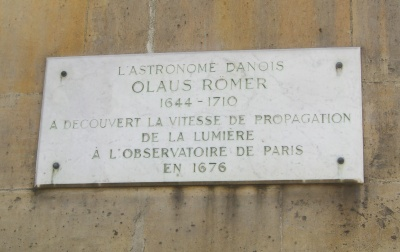
\includegraphics[max width=0.65\linewidth]{../images/paris_observatory_romer_speed_of_light.jpg}\]
Later, Henri Poincaré worked for the French Bureau of Longitude. Among
other things, he was the scientific secretary for its mission to
Ecuador.

To keep track of time precisely all over the world, you need to think
about the finite speed of light. This may have spurred Poincaré's work
on relativity! Here's a good book that argues this case:

\begin{enumerate}
\def\labelenumi{\arabic{enumi})}
\setcounter{enumi}{2}
\tightlist
\item
  Peter Galison, \emph{Einstein's Clocks, Poincaré's Maps: Empires of
  Time}, W. W. Norton, New York, 2003. Reviewed by Robert Wald in
  Physics Today at
  \texttt{http://www.physicstoday.org/vol-57/iss-9/p57.html}
\end{enumerate}

I met Galison in Delphi, and it's clear he like to think about the
impact of practical stuff on math and physics.

I was in Delphi for a meeting of ``Thales and Friends'':

\begin{enumerate}
\def\labelenumi{\arabic{enumi})}
\setcounter{enumi}{3}
\tightlist
\item
  ``Thales and Friends'', \texttt{http://www.thalesandfriends.org}
\end{enumerate}

This is an organization that's trying to bridge the gap between
mathematics and the humanities. It's led by Apostolos Doxiadis, who is
famous for this novel:

\begin{enumerate}
\def\labelenumi{\arabic{enumi})}
\setcounter{enumi}{4}
\tightlist
\item
  Apostolos Doxiadis, \emph{Uncle Petros and Goldbach's Conjecture},
  Bloomsbury, New York, 2000. Review by Keith Devlin at
  \texttt{http://www.maa.org/reviews/petros.html}
\end{enumerate}

There's a lot I could say about this meeting, but I just want to
advertise a forthcoming book by Doxiadis and a computer scientist friend
of his. It's a comic book --- sorry, I mean ``graphic novel''! --- about
the history of mathematical logic from Russell to Goedel:

\begin{enumerate}
\def\labelenumi{\arabic{enumi})}
\setcounter{enumi}{5}
\tightlist
\item
  Apostolos Doxiadis and Christos Papadimitriou, \emph{Logicomix}, to
  appear.
\end{enumerate}

I saw a partially finished draft. I think it does a good job of
explaining to nonmathematicians what the big deal was with mathematical
logic around the turn of the last century\ldots{} and how these ideas
eventually led to computers. It's also a fun story.

If you're eager for summer reading and can't wait for Logicomix, you
might try this other novel by Papadimitrou:

\begin{enumerate}
\def\labelenumi{\arabic{enumi})}
\setcounter{enumi}{6}
\tightlist
\item
  Christos Papadimitriou, \emph{Turing (a Novel about Computation)}, MIT
  Press, Boston, 2003.
\end{enumerate}

It's a history of mathematics from the viewpoint of computer science, as
told by a computer program named Turing to a lovelorn archaeologist. I
haven't seen it yet.

Okay --- enough fun stuff. On to the Abel Symposium!

\begin{enumerate}
\def\labelenumi{\arabic{enumi})}
\setcounter{enumi}{7}
\tightlist
\item
  Abel Symposium 2007, \texttt{http://abelsymposium.no/2007}
\end{enumerate}

Actually this was a lot of fun too. A bunch of bigshots were there,
including a bunch who didn't even give talks, like Eric Friedlander, Ib
Madsen, Jack Morava, and Graeme Segal.

(My apologies to all the bigshots I didn't list.)

Speaking of bigshots, Vladimir Voevodsky gave a special surprise lecture
on symmetric powers of motives. He wowed the audience not only with his
mathematical powers but also his ability to solve a technical problem
that had stumped all the previous speakers! The blackboards in the
lecture hall were controlled electronically, by a switch. But, the
blackboards only moved a few inches before stalling out. So, people had
to keep hitting the switch over and over. It was really annoying, and it
became the subject of running jokes. People would ask the speakers:
``Can't you talk and press buttons at the same time?''

So, what did Voevodsky do? He lifted the blackboard by hand! He laughed
and said ``Russian solution''. But, I think it's a great example of how
he gets around problems by creative new approaches.

It really pleased me how many talks mentioned \(n\)-categories, and even
used them to do exciting things. This seems quite new. In the old days,
bigshots might think about \(n\)-categories, but they'd be embarrassed
to actually mention them, since they had a reputation for being ``too
abstract''.

In fact, Dan Freed alluded to this in his talk on topological quantum
field theory. He said that every mathematician has an ``\(n\)-category
number''. Your \(n\)-category number is the largest \(n\) such that you
can think about \(n\)-categories for a half hour without getting a
splitting headache.

When Freed first invented this concept, he felt pretty self-satisfied,
since his \(n\)-category number was \(1\), while for most mathematicians
it was \(0\). But lately, he says, other people's \(n\)-category numbers
have been increasing, while his has stayed the same.

He said this makes him suspicious. In light of the scandals plaguing the
Tour de France and American baseball, he suspects mathematicians are
taking ``category-enhancing substances''!

Freed shouldn't feel bad: he was among the first to introduce
\(n\)-categories in the subject of topological quantum field theory! He
gave a nice talk on this, clear and unpretentious, leading up to a
conjecture for the \(3\)-vector space that Chern-Simons theory assigns
to a point.

That would make a great followup to these papers on the \(2\)-vector
space that Chern-Simons theory assigns to a circle:

\begin{enumerate}
\def\labelenumi{\arabic{enumi})}
\setcounter{enumi}{8}
\item
  Daniel S. Freed, ``The Verlinde algebra is twisted equivariant
  K-theory'', available as
  \href{http://arxiv.org/abs/math/0101038}{\texttt{arXiv:math/0101038}}.

  Daniel S. Freed, ``Twisted K-theory and loop groups'', available as
  \href{http://arxiv.org/abs/math/0206237}{\texttt{arXiv:math/0206237}}.

  Daniel S. Freed, Michael J. Hopkins and Constantin Teleman, ``Loop
  groups and twisted K-theory II'', available as
  \href{http://arxiv.org/abs/math/0511232}{\texttt{arXiv:math/0511232}}.

  Daniel S. Freed, Michael J. Hopkins and Constantin Teleman, ``Twisted
  K-theory and loop group representations'', available as
  \href{http://arxiv/abs/math/0312155}{\texttt{arXiv:math/0312155}}.
\end{enumerate}

In a similar vein, Jacob Lurie talked about his work with Mike Hopkins
in which they proved a version of the ``Baez-Dolan cobordism
hypothesis'' in dimensions 1 and 2. I'm calling it this because that's
what Lurie called it in his title, and it makes me feel good.

You can read about this hypothesis here:

\begin{enumerate}
\def\labelenumi{\arabic{enumi})}
\setcounter{enumi}{9}
\tightlist
\item
  John Baez and James Dolan, ``Higher-dimensional algebra and
  topological quantum field theory'', \emph{J. Math. Phys.} \textbf{36}
  (1995) 6073--6105. Also available as
  \href{https://arxiv.org/abs/q-alg/9503002}{\texttt{q-alg/9503002}}.
\end{enumerate}

It was an attempt to completely describe the algebraic structure of the
\(n\)-category \(n\mathsf{Cob}\), where:

\begin{itemize}
\tightlist
\item
  objects are 0d manifolds,
\item
  \(1\)-morphisms are 1d manifolds with boundary,
\item
  \(2\)-morphisms are 2d manifolds with corners,
\item
  \(3\)-morphisms are 3d manifolds with corners,
\item
  \ldots{}
\end{itemize}

and so on up to dimension \(n\). Unfortunately, at the time we proposed
it, little was known about \(n\)-categories above \(n = 3\). For a more
recent take on these ideas, see:

\begin{enumerate}
\def\labelenumi{\arabic{enumi})}
\setcounter{enumi}{10}
\tightlist
\item
  Eugenia Cheng and Nick Gurski, ``Towards an \(n\)-category of
  cobordisms'', \emph{Theory and Applications of Categories} \textbf{18}
  (2007), 274--302. Available at
  \texttt{http://www.tac.mta.ca/tac/volumes/18/10/18-10abs.html}
\end{enumerate}

Lurie and Hopkins use a new trick: they redefine \(n\mathsf{Cob}\) to be
a special sort of \(\infty\)-category. The idea is to use
diffeomorphisms and homotopies between these as morphisms above
dimension \(n\). This gives an \(\infty\)-category version of
\(n\mathsf{Cob}\), where:

\begin{itemize}
\tightlist
\item
  objects are \(0\)-dimensional manifolds,
\item
  \(1\)-morphisms are \(1\)-dimensional manifolds with boundary,
\item
  \(2\)-morphisms are \(2\)-dimensional manifolds with corners,
\item
  \(3\)-morphisms are \(3\)-dimensional manifolds with corners,
\item
  \ldots{}
\item
  \(n\)-morphisms are \(n\)-dimensional manifolds with corners,
\item
  \((n+1)\)-morphisms are diffeomorphisms,
\item
  \((n+2)\)-morphisms are homotopies between diffeomorphisms,
\item
  \((n+3)\)-morphisms are homotopies between homotopies,
\item
  \ldots{}
\end{itemize}

and so on for ever!

Since everything here is invertible above dimension \(n\), this is
called an ``\((\infty,n)\)-category''.

This sounds worse than an \(n\)-category, but it's okay for small \(n\).
In particular, \((\infty,1)\)-categories are pretty well understood by
now. There are a bunch of different approaches, with scary names like
``topological categories'', ``simplicial categories'', ``\(A_\infty\)
categories'', ``Segal categories'', ``complete Segal spaces'', and
``quasicategories''. Luckily, all these approaches are known to be
equivalent --- see \protect\hyperlink{week245}{``Week 245''} for some
good introductory material by Julie Bergner and Andre Joyal. Joyal is
now writing a book on this stuff.

Lurie is a real expert on \((\infty,1)\)-categories. In fact, starting
as a grad student, he wrote a mammoth tome generalizing topos theory
from categories to \((\infty,1)\)-categories:

\begin{enumerate}
\def\labelenumi{\arabic{enumi})}
\setcounter{enumi}{11}
\tightlist
\item
  Jacob Lurie, ``Higher topos theory'', available as
  \href{http://arxiv.org/abs/math/0608040}{\texttt{arXiv:math/0608040}}.
\end{enumerate}

I'm sure Freed would suspect him of taking category-enhancing
substances: his category number is infinite, and this book is 619 pages
long! Then he went on to apply this stuff to algebraic geometry\ldots{}
and the world is still reeling. I was happy to discover that he's a nice
guy, enthusiastic and friendly --- not the terrifying fiend I expected.

Anyway, Lurie and Hopkins have worked out the precise structure of the
\((\infty,1)\)-category version of \(1\mathsf{Cob}\), and also the
\((\infty,2)\)-category version of \(2\mathsf{Cob}\). Unfortunately this
work is not yet written up. But, they use results from this paper:

\begin{enumerate}
\def\labelenumi{\arabic{enumi})}
\setcounter{enumi}{12}
\tightlist
\item
  Soren Galatius, Ib Madsen, Ulrike Tillmann, Michael Weiss, ``The
  homotopy type of the cobordism category'', available as
  \href{http://arxiv.org/abs/math/0605249}{\texttt{arXiv:math/0605249}}.
\end{enumerate}

And, Ulrike Tillmann gave a talk about this paper! It computes the
``nerve'' of the \((\infty,1)\)-category where:

\begin{itemize}
\tightlist
\item
  objects are \((n-1)\)-dimensional manifolds,
\item
  \(1\)-morphisms are \(n\)-dimensional manifolds with boundary,
\item
  \(2\)-morphisms are diffeomorphisms,
\item
  \(3\)-morphisms are homotopies between diffeomorphisms,
\item
  \(4\)-morphisms are homotopies between homotopies,
\item
  \ldots{}
\end{itemize}

The ``nerve'' is a trick for turning any sort of \(\infty\)-category
into a space, or simplicial set. (See item J of
\protect\hyperlink{week117}{``Week 117''} for the nerve of a plain old
category. This should give you the general idea.)

In her talk, she went further and computed the nerve of the
\((\infty,k)\)-category where:

\begin{itemize}
\tightlist
\item
  objects are \((n-k)\)-dimensional manifolds,
\item
  \(1\)-morphisms are \((n-k+1)\)-dimensional manifolds with boundary,
\item
  \(2\)-morphisms are \((n-k+2)\)-dimensional manifolds with corners,
\item
  \ldots{}
\item
  \(k\)-morphisms are \(n\)-dimensional manifolds with corners,
\item
  \((k+1)\)-morphisms are diffeomorphisms,
\item
  \((k+2)\)-morphisms are homotopies between diffeomorphisms,
\item
  \((k+3)\)-morphisms are homotopies between homotopies,
\item
  \ldots{}
\end{itemize}

This is also joint work with the same coauthors, but it seems not to be
written up yet, except for \(k = 1\), where it's proved in the above
paper. The cool thing about the new work is that it uses an idea
familiar from higher category theory --- a \(k\)-simplicial space --- to
give a rigorous description of the nerve of the above
\((\infty,k)\)-category! Indeed, Tillmann told me she thinks of
\(k\)-simplicial spaces as just a convenient way of dealing with higher
categories.

Stephan Stolz's talk also involved cobordism \(n\)-categories, but I'll
say more about that later.

Ralph Cohen and Dennis Sullivan both gave talks on string topology --- a
trick for studying a space by studying collections of loops in that
space, and relating this to ideas from string theory.

String topology started when Chas and Sullivan took the ideas of string
theory and applied them in a somewhat ethereal form to strings
propagating in any manifold.

In full-fledged string theory, one of the main tools is ``conformal
field theory''. In a CFT, if you have a state of \(n\) strings, and a
Riemann surface going from \(n\) strings to \(m\) strings, you get a
state of \(m\) strings.

A good way to get CFTs is to consider strings propagating on some
manifold or other. Of course the manifold needs some sort of geometry,
like a Riemannian metric, for your strings to know how to propagate.

But Chas and Sullivan figured out what you can do if the spacetime is a
bare manifold, without any metric. Basically, you just need to stick the
word ``homology'' in front of everything! This makes everything
sufficiently floppy.

So, instead of considering actual loops in a manifold \(M\), which form
a space \(LM\), they took the homology of \(LM\) and got a vector space
or abelian group \(H(LM)\). Then, for each homology class \(C\) on the
moduli space of Riemann surfaces that go from \(n\) circles to \(m\)
circles, they got an operation with \(n\) inputs and \(m\) outputs:
\[Z(C)\colon H(LM)^{\otimes n} \to H(LM)^{\otimes m}\] All these
operations fit together into a slight generalization of an operad,
called a ``PROP''.

If you don't remember what an ``operad'' is, give yourself twenty lashes
with a wet noodle and review \protect\hyperlink{week220}{``Week 220''}.
Suitably punished, you can then enjoy this:

\begin{enumerate}
\def\labelenumi{\arabic{enumi})}
\setcounter{enumi}{13}
\tightlist
\item
  Ralph Cohen and Alexander Voronov, ``Notes on string topology'',
  available as
  \href{http://arxiv.org/abs/math/0503625}{\texttt{arXiv:math/0503625}}.
\end{enumerate}

Both PROPs and operads are defined near the beginning here. PROPs and
operads are gadgets for describing operations with any number of inputs.
Operads can only handle operations with one output. PROPS can handle
operations with any number of outputs.

To see a more geometrical treatment of string topology, the way it
looked before the operadchiks got ahold of it, try the original paper by
Chas and Sullivan:

\begin{enumerate}
\def\labelenumi{\arabic{enumi})}
\setcounter{enumi}{14}
\tightlist
\item
  Moira Chas and Dennis Sullivan, ``String topology'', available as
  \href{http://arxiv.org/abs/math/9911159}{\texttt{arXiv:math/9911159}}.
\end{enumerate}

Sullivan talked about some recent refinements of string topology which
deal with the fact that the moduli space of Riemann surfaces has a
``boundary'', so it doesn't have a closed ``top-dimensional homology
class''.

Cohen's talk described some cool relations between string topology and
symplectic geometry! In physics we use symplectic manifolds to describe
the space of states --- the so-called ``phase space'' --- of a classical
system. So, if you have a loop in a symplectic manifold, it can describe
a periodic orbit of some classical system. In particular, if we pick a
periodic time-dependent Hamiltonian for this system, a loop will be a
solution of Hamilton's equations iff it's a critical point for the
``action''.

But, we can also imagine letting loops move in the direction of
decreasing action, following the ``gradient flow''. They'll trace out 2d
surfaces which we can think of as string world-sheets! This is just what
string topology studies, but now we can get ``Morse theory'' into the
game: this studies a space (here \(LM\)) by looking at critical points
of a function on this space, and its gradient flow.

So, we get a nice interaction between periodic orbits in phase space,
and the string topology of that space, and Morse theory! For more, try
this:

\begin{enumerate}
\def\labelenumi{\arabic{enumi})}
\setcounter{enumi}{15}
\tightlist
\item
  Ralph Cohen, ``The Floer homotopy type of the cotangent bundle'',
  available as
  \href{http://arxiv.org/abs/math/0702852}{\texttt{arXiv:math/0702852}}.
\end{enumerate}

Next, let me say a bit about Stephan Stolz's talk. He spoke on his work
with Peter Teichner, which is a very ambitious attempt to bring quantum
field theory right into the heart of algebraic topology.

I discussed this in \protect\hyperlink{week197}{``Week 197''}. I said
they were working on a wonderful analogy between quantum field theories
and different flavors of cohomology. It's been published since then:

\begin{enumerate}
\def\labelenumi{\arabic{enumi})}
\setcounter{enumi}{16}
\tightlist
\item
  Stephan Stolz and Peter Teichner, ``What is an elliptic object?''
  Available at
  \texttt{http://math.berkeley.edu/\textasciitilde{}teichner/papers.html}
\end{enumerate}

Back then, the analogy looked like this:

\begin{longtable}[]{@{}ll@{}}
\toprule
\endhead
\(1\)-dimensional supersymmetric QFTs & complex K-theory\tabularnewline
\(2\)-dimensional supersymmetric conformal QFTs & elliptic
cohomology\tabularnewline
\bottomrule
\end{longtable}

When I saw this, I tried to guess a generalization to higher dimensions.

There's an obvious guess for the right-hand column, since there's
something called the ``chromatic filtration'', which is --- very roughly
- a list of cohomology theories. Complex K-theory is the 1st entry on
this list, and elliptic cohomology is the 2nd! (For a lot more details,
see \protect\hyperlink{week149}{``Week 149''} and
\protect\hyperlink{week150}{``Week 150''}.)

There's also an obvious guess for the left-hand column:
\(n\)-dimensional supersymmetric QFTs of some sort!

The problem is the word ``conformal'' in the second row. In 2
dimensions, a conformal structure is a way of making spacetime look
locally like the complex plane. This is great, because elliptic
cohomology has a lot to do with complex analysis --- or more precisely,
elliptic curves and modular forms. But, it's not clear how one should
generalize this to higher dimensions!

Luckily, thanks to a subsequent conversation with Witten, Stolz and
Teichner realized that the partition function of a 2d supersymmetric QFT
gives a modular form even if the QFT is not invariant under conformal
transformations. This means we can remove the word ``conformal'' from
the second row! For more details, try this:

\begin{enumerate}
\def\labelenumi{\arabic{enumi})}
\setcounter{enumi}{17}
\tightlist
\item
  Stephan Stolz and Peter Teichner, ``Super symmetric field theories and
  integral modular forms'', preliminary version available at
  \texttt{http://math.berkeley.edu/\textasciitilde{}teichner/papers.html}
\end{enumerate}

They've also gone back and added a 0th row to their chart. It's always
wise to start counting at zero! Now the chart looks much nicer:

\begin{longtable}[]{@{}ll@{}}
\toprule
\endhead
\(0\)-dimensional supersymmetric QFTs & deRham cohomology\tabularnewline
\(1\)-dimensional supersymmetric QFTs & complex K-theory\tabularnewline
\(2\)-dimensional supersymmetric QFTs & elliptic
cohomology\tabularnewline
\bottomrule
\end{longtable}

Yes, good old deRham cohomology is the 0th entry in the ``chromatic
filtration''! It's the least scary sort of cohomology theory, at least
for physicists. They get scarier as we move down the chart.

Quantum field theory also gets scarier as we move down the chart --- the
infinities that plague quantum field theory tend to get worse in higher
dimensions of spacetime. So, while we can dream about extensions of this
chart, there's already plenty to handle here.

The most audacious idea in Stolz and Teichner's work is to take a
manifold \(X\) and study the set of all \(n\)-dimensional QFT's
``parametrized by \(X\)''.

For \(X\) a point, such a thing is just an ordinary \(n\)-dimensional
QFT. Roughly speaking, this is a gadget \(Z\) that assigns:

\begin{itemize}
\tightlist
\item
  a Hilbert space \(Z(S)\) to any \((n-1)\)-dimensional Riemannian
  manifold \(S\);
\item
  a linear operator \(Z(M)\colon Z(S) \to Z(S')\) to any
  \(n\)-dimensional Riemannian manifold \(M\) going from \(S\) to
  \(S'\).
\end{itemize}

If you're a mathematician, you may know that \(M\) is really a
``cobordism'' from \(S\) to \(S'\), written \(M\colon S \to S'\). And if
you're really cool, you'll know that cobordisms form a symmetric
monoidal category \(n\mathsf{Cob}\), and that \(Z\) should be a
symmetric monoidal functor.

If you're a physicist, you'll know that \(S\) stands for ``space'' and
``\(M\)'' stands for ``spacetime''. All the stuff I'm describing should
remind you of the definition of a ``TQFT'', except now our spaces and
spacetimes have Riemannian metrics, because we're doing honest QFTs, not
topological ones.

Given a spacetime \(M\), we try to compute the operator \(Z(M)\) as a
path integral; for example, an integral over all maps
\[f\colon M \to T\] where \(f\) is a ``field'' taking values in a
``target space'' \(T\).

If this seems too scary, take \(n = 1\). Then we've got a
\(1\)-dimensional quantum field theory, so we can take our spacetime
\(M\) to be an interval. Then \(f\) is just a path in some space \(T\).
In this case the path integral is really an integral over all paths a
particle could trace out in \(T\). So, \(1\)-dimensional quantum field
theory is just ordinary quantum mechanics!

There are a lot of subtleties I'm skipping over here, both on the math
and physics sides. But never mind --- the really cool part is this
generalization:

Roughly speaking, an \(n\)-dimensional QFT ``parametrized by \(X\)''
assigns:

\begin{itemize}
\tightlist
\item
  a Hilbert space \(Z(S)\) to any \((n-1)\)-dimensional Riemannian
  manifold \(S\) \emph{equipped with a map} \(g\colon S \to X\);
\item
  a linear operator \(Z(M)\colon Z(S) \to Z(S')\) to any
  \(n\)-dimensional Riemannian cobordism \(M\colon S \to S'\)
  \emph{equipped with a map} \(g\colon M \to X\).
\end{itemize}

If you're a mathematician, you may see we've switched to using
cobordisms ``over \(X\)''. It's a straightforward generalization.

But what does it mean physically? Here the path integral picture is
helpful. Now we're doing a path integral over all fields
\[f\colon M \to T \times X\] where we demand that the second component
of this function is \[g\colon M \to X\] For example, if we've got a 1d
QFT, we're letting a particle roam over \(T \times X\), but demanding
that its \(X\) coordinates follow a specific path \(g\).

So, we're doing a \emph{constrained} path integral!

In heaven, everything physicists do can be made mathematically rigorous.
Up there, knowing how to do these constrained path integrals would tell
us how to do unconstrained path integrals: we'd just integrate over all
choices of the path \(g\). So, a QFT parametrized by \(X\) would
automatically give us an ordinary QFT.

Now, an ordinary QFT is just a QFT parametrized by a point! So, if we
use \(\mathrm{QFT}(X)\) to mean the set of \(n\)-dimensional QFTs
parametrized by \(X\), we'd have a map
\[\mathrm{QFT}(X) \to \mathrm{QFT}(\mathrm{point})\] This is called
``pushing forward to a point''.

More generally, we could hope that any map \[F\colon X \to X'\] gives a
``pushforward'' map \[F_*\colon \mathrm{QFT}(X) \to \mathrm{QFT}(X')\]
Let's see if this makes any sense. In fact, I've been overlooking some
important issues. An example will shed light on this.

Consider a \(0\)-dimensional QFT parametrized by some manifold \(X\).
Let's call it \(Z\). What is \(Z\) like, concretely?

For starters, notice that the only \((-1)\)-dimensional manifold is the
empty set. A \(0\)-dimensional manifold ``going from the empty set to
the empty set'' is just a set of points. Also, while I didn't mention it
earlier, all manifolds in this game must be \emph{compact}. So, this set
of points must be finite.

If you now take the definition I wrote down and use that ``symmetric
monoidal functor'' baloney, you'll see \(Z\) assigns a \emph{number} to
any finite set of points mapped into \(X\). Furthermore, this assignment
must be multiplicative. So, it's enough to know a number for each point
in \(X\). In short, our QFT is just a function:
\[Z\colon X \to \mathbb{C}\] Now suppose we map \(X\) to a point:
\[F\colon X \to \mathrm{point}\] What should the pushforward
\[F_*\colon \mathrm{QFT}(X) \to \mathrm{QFT}(\mathrm{point})\] do to the
function \(Z\)?

There's an obvious guess: we should \emph{integrate} this function on
\(X\) to get a number --- that is, a function on a point. Indeed, that's
what ``path integration'' should reduce to in this pathetically simple
case: plain old integration!

Alas, there's no good way to integrate a function over \(X\) unless this
manifold comes equipped with a measure. But, if \(X\) is compact,
oriented and \(p\)-dimensional, we can integrate a \emph{\(p\)-form}
over \(X\).

More generally, if we have a bundle \[F\colon X \to X'\] with compact
\(d\)-dimensional fibers, we can take a \(p\)-form on \(X\) and
integrate it over the fibers to get a \((p-d)\)-form on \(X'\). This is
how you ``push forward'' differential forms.

So, pushing forward is a bit subtler than I led you to believe at first.
We should really talk about \(n\)-dimensional QFTs ``of degree \(p\)''
parametrized by \(X\). Let's call the set of these \[\mathrm{QFT}^p(X)\]
I won't define them, but for \(n = 0\) they're just \(p\)-forms on
\(X\). Anyway: if we have a bundle \[F\colon X \to X'\] with compact
\(d\)-dimensional fibers, we can hope there's a pushforward map
\[F_*\colon \mathrm{QFT}^p(X) \to \mathrm{QFT}^{p-d}(X')\] There should
also be a pullback map
\[F^*\colon \mathrm{QFT}^p(X') \to \mathrm{QFT}^p(X)\] This is a lot
less tricky, and I'll let you figure out how it works.

I should warn you, I've been glossing over lots of important aspects of
this work --- like the role played by \(n\)-categories, and the role
played by supersymmetry. Supersymmetry doesn't matter much for the broad
conceptual picture I've been sketching. But, we need it for this analogy
to work:

\begin{longtable}[]{@{}ll@{}}
\toprule
\endhead
\(0\)-dimensional supersymmetric QFTs & deRham cohomology\tabularnewline
\(1\)-dimensional supersymmetric QFTs & complex K-theory\tabularnewline
\(2\)-dimensional supersymmetric QFTs & elliptic
cohomology\tabularnewline
\bottomrule
\end{longtable}

The idea is to impose an equivalence relation on supersymmetric QFTs,
called ``concordance'', and try to show:

\begin{itemize}
\tightlist
\item
  The set of concordance classes of degree-\(p\) 0d supersymmetric QFTs
  parametrized by \(X\) is the \(p\)th de Rham cohomology group of
  \(X\).
\item
  The set of concordance classes of degree-\(p\) 1d supersymmetric QFTs
  parametrized by \(X\) is the \(p\)th K-theory group of \(X\).
\item
  The set of concordance classes of degree-\(p\) 2d supersymmetric QFTs
  parametrized by \(X\) is the \(p\)th elliptic cohomology group of
  \(X\).
\end{itemize}

So far people have done this in the 0d and 1d cases. The 2d case is a
major project, because it pushes the limits of what people can do with
quantum field theory.

Why did I spend so much time talking about pushforwards of QFTs? Well,
it's very important for defining invariants like the ``fundamental
class'' of an oriented manifold, or the ``\(\hat{A}\) genus'' of a spin
manifold, or the ``Witten index'' of a string manifold.

Here's how it goes, very roughly. Suppose \(X\) is a compact Riemannian
manifold. Then the simplest \(n\)-dimensional QFT parametrized by \(X\)
is the one where we take the target space \(T\) (mentioned a while back)
to be just a point!

This parametrized QFT is called the ``nonlinear \(\sigma\)-model'', for
stupid historic reasons. All the fun happens when we push this QFT
forwards to a point. Then we integrate over all the maps
\(g\colon M \to X\). The result --- usually called the ``partition
function'' of the nonlinear \(\sigma\)-model --- should be an
interesting invariant of \(X\).

In the case \(n = 1\), this trick gives the ``\(\hat{A}\) genus'' of
\(X\), but it only works when \(X\) is a spin manifold: we need this to
define the 1d supersymmetric nonlinear \(\sigma\)-model.

In the case \(n = 2\), this trick gives the ``Witten genus'' of \(X\),
but it only works when \(X\) is a string manifold: we need this to
define the 2d supersymmetric nonlinear \(\sigma\)-model.

For more on the \(n = 1\) case, see:

\begin{enumerate}
\def\labelenumi{\arabic{enumi})}
\setcounter{enumi}{18}
\tightlist
\item
  Henning Hohnhold, Peter Teichner and Stephan Stolz, ``From minimal
  geodesics to super symmetric field theories''. In memory of Raoul
  Bott. Available at
  \texttt{http://math.berkeley.edu/\textasciitilde{}teichner/papers.html}
\end{enumerate}

For the \(n = 2\) case, see the papers I already listed.

(I'm confused about the case \(n = 0\), for reasons having to do with
the ``degree'' I mentioned earlier.)

Finally: the cool part, which I haven't even mentioned, is that we
really need to describe \(n\)-dimensional QFTs using an
\emph{\(n\)-category} of cobordisms --- not just a mere \(1\)-category,
as I sloppily said above.

This first gets exciting when we hit \(n = 2\): you'll see a bunch of
stuff about \(2\)-categories (or technically, ``bicategories'') in the
old Stolz-Teichner paper ``What is an elliptic object'', listed above.

In short: we're starting to see a unified picture where we study spaces
by letting particles, strings, and their \(n\)-dimensional cousins roam
around in these spaces. There are lots of slight variants: string
topology, the Stolz-Teichner picture, and of course good old-fashioned
topological quantum field theory. All of them have a lot to do with
\(n\)-categories.

There's a lot more to say about all this\ldots{} but luckily, there
should be a proceedings of this conference, where you can read more. My
own talk is here:

\begin{enumerate}
\def\labelenumi{\arabic{enumi})}
\setcounter{enumi}{19}
\tightlist
\item
  John Baez, ``Higher gauge theory and elliptic cohomology'',
  \texttt{http://math.ucr.edu/home/baez/abel/}
\end{enumerate}

It, too, is about studying spaces by letting strings roam around inside
them!

But instead of summarizing my own talk, I want to say a bit about the
other side of the symposium --- the motivic cohomology side!

I'll only summarize a few basic definitions. I got these from the talks
by Fabian Morel and Vladimir Voevodsky, and I want to write them down
before I forget! For more, try these:

\begin{enumerate}
\def\labelenumi{\arabic{enumi})}
\setcounter{enumi}{20}
\item
  Fabian Morel and Vladimir Voevodsky, \(A^1\)-homotopy theory of
  schemes, September 1998. Available at
  \texttt{http://citeseer.ist.psu.edu/morel98suphomotopy.html}
\item
  Vladimir Voevodsky (notes by Charles Weibel), ``Voevodsky's Seattle
  Lectures: K-theory and motivic cohomology''. Available at
  \texttt{http://citeseer.ist.psu.edu/249068.html}
\end{enumerate}

Okay:

\(A^1\)-homotopy theory is an attempt to do homotopy theory for
algebraic geometry. In algebraic geometry we often work over a fixed
field \(k\), and the goal here is to create a category which contains
smooth algebraic varieties over \(k\) as objects, but also other more
general spaces, providing a sufficiently flexible category in which to
do homotopy theory.

One of the simplest smooth algebraic varieties over \(k\) is the
``affine line'' \(A^1\). The algebraic functions on this line are just
polynomials in one variable with coefficients in \(k\). In
\(A^1\)-homotopy theory, we want to set up a context where we can use
the affine line \(A^1\) to parametrize homotopies, much as we use the
unit interval \([0,1]\) in ordinary homotopy theory.

For this, people start by looking at \(\mathsf{Sm}(k)\), the category of
smooth algebraic varieties over \(k\). Then, they consider the category
of ``simplicial presheaves'' on \(\mathsf{Sm}(k)\).

A simplicial presheaf on \(\mathsf{Sm}(k)\) is just a functor
\[F\colon \mathsf{Sm}(k)^\mathrm{op} \to \mathsf{SimpSet}\] where
\(\mathsf{SimpSet}\) is the category of simplicial sets (see item C of
\protect\hyperlink{week115}{``Week 115''}) We think of \(F\) as
specifying some sort of space by telling us for each smooth algebraic
variety \(X\) the simplicial set \(F(X)\) of all maps into this space.

To make this kind of abstract space work nicely, \(F(X)\) should depend
``locally'' on \(X\). For this, we insist that given a cover of a
variety \(X\) by varieties \(U_i\), guys in \(F(X)\) are the same as
guys in \(F(U_i)\) that agree on the intersections \[U_i \cap U_j.\]
Here ``cover'' means ``cover in the Nisnevich topology'' --- that is, an
étale cover such that every point being covered is the image of a point
in the cover for which the covering map induces an isomorphism of
residue fields.

If you've come this far, you may not be scared to hear that the
Nisnevich topology is really a ``Grothendieck topology'' on
\(\mathsf{Sm}(k)\), and I'm really demanding that \(F\) be a ``sheaf''
with respect to this topology.

So, the kind of ``space'' we're studying is a simplicial sheaf on the
category of smooth varieties over \(k\) with its Nisnevich topology. We
call these category of these guys \(\mathsf{Space}(k)\).

Just saying this already makes me feel smart. Just think how smart I'd
feel if I knew why the Nisnevich topology was better than the good old
étale topology!

Anyway, to do homotopy theory with these simplicial sheaves, we need to
make \(\mathsf{Space}(k)\) into a ``model category''. I should have
explained model categories in some previous Week, but I've never gotten
around to it, and right now is not the time. So, I'll just say one key
thing.

The \emph{most} important thing about a model category is that it's
equipped with a collection of morphisms that act like homotopy
equivalences. They're called ``weak equivalences''.

Already in ordinary topology, these weak equivalences are a slight
generalization of homotopy equivalences. They're actually the same as
homotopy equivalences when the spaces involved are nice; they're
designed to work better for nasty spaces.

In \(A^1\)-homotopy theory, the weak equivalences are generated by two
kinds of morphisms:

\begin{itemize}
\tightlist
\item
  the projection maps \(X \times A^1 \to X\)
\item
  the maps \(\check{\mathcal{C}}(\mathcal{U}) \to X\) coming from covers
  \(\mathcal{U}\) of \(X\).
\end{itemize}

Here \(X\) is any space in \(\mathsf{Space}(k)\), and
\(\check{\mathcal{C}}(\mathcal{U})\) is the ``Cech nerve'' of the cover
\(\mathcal{U}\).

This framework seems like a really cool blend of algebraic geometry and
homotopy theory. But, to do homology theory in a good way we need to go
a bit further, and introduce ``motives''.

However, I'm tired, and I bet you are too! Motives are a big idea, and
it doesn't make sense to start talking about them now. So, some other
day\ldots.

\begin{center}\rule{0.5\linewidth}{0.5pt}\end{center}

\textbf{Addendum:} For more discussion, go to the
\href{http://golem.ph.utexas.edu/category/2007/08/this_weeks_finds_in_mathematic_16.html}{\(n\)-Category
Café}.

\begin{center}\rule{0.5\linewidth}{0.5pt}\end{center}

\begin{quote}
\emph{And if a bird can speak, who once was a dinosaur, and a dog can
dream, should it be implausible that a man might supervise the
construction of light?}

--- King Crimson
\end{quote}



\hypertarget{week256}{%
\section{August 27, 2007}\label{week256}}

My European wanderings continue. I'm in Greenwich again, just back from
a mind-blowing conference in Vienna, part of a bigger program that's
still going on:

\begin{enumerate}
\def\labelenumi{\arabic{enumi})}
\tightlist
\item
  \emph{Poisson sigma models, Lie algebroids, deformations, and higher
  analogues}, Erwin Schrödinger Institute, August -- September 2007,
  organized by Thomas Strobl, Henrique Bursztyn, and Harald Grosse.
  Program at
  \texttt{http://w3.impa.br/\textasciitilde{}henrique/esi.html}
\end{enumerate}

I learned a huge amount, both from the talks and from conversations with
Urs Schreiber and others. Mainly, I learned that I've really been
falling behind the times when it comes to classical mechanics and
quantization!

I could easily spend several Weeks trying to assimilate the
half-digested information I acquired and explain it all to you. But, I
want to get back to the Tale of Groupoidification! So, I'll only say a
little about this wonderful conference.

You may know that in classical mechanics, the space of states of a
physical system is called its ``phase space''. Often this is described
by a ``symplectic manifold'' --- a manifold equipped with a
nondegenerate closed \(2\)-form. Sometimes it's described by a ``Poisson
manifold'' --- a manifold equipped with a bracket operation on its
smooth functions, making the smooth functions into a Lie algebra and
also satisfying the product rule: \[\{f,gh\} = \{f,g\}h + g\{f,h\}\]
Every symplectic manifold gives a Poisson manifold, but not vice versa.
A good example of a Poisson manifold that's not symplectic is the phase
space of a spinning point particle, which has angular momentum but no
other properties.

Every mathematical physicist should know some symplectic geometry and
Poisson geometry! To get started on symplectic geometry, try these, in
rough order of increasing difficulty:

\begin{enumerate}
\def\labelenumi{\arabic{enumi})}
\item
  Vladimir I. Arnold, \emph{Mathematical Methods of Classical
  Mechanics}, Springer, Berlin, 1997.
\item
  Ralph Abraham and Jerrold E. Marsden, \emph{Foundations of Mechanics},
  Benjamin-Cummings, New York, 1978.
\item
  Victor Guillemin and Shlomo Sternberg, \emph{Symplectic Techniques in
  Physics}, Cambridge U. Press, Cambridge, 1990.
\item
  Ana Cannas da Silva, \emph{Symplectic geometry}, available as
  \href{http://arxiv.org/abs/math.SG/0505366}{\texttt{arXiv:math.SG/0505366}}.
\item
  Sergei Tabachnikov, \emph{Introduction to symplectic topology},
  available at
  \texttt{http://www.math.psu.edu/tabachni/courses/symplectic.pdf}
\end{enumerate}

For Poisson geometry, try the above but also:

\begin{enumerate}
\def\labelenumi{\arabic{enumi})}
\setcounter{enumi}{5}
\item
  Alan Weinstein, \emph{Poisson geometry}, available at
  \texttt{http://galileo.stmarys-ca.edu/bdavis/poisson.pdf}
\item
  Darryl Holm, ``Applications of Poisson geometry to physical
  problems'', available as
  \href{http://arxiv.org/abs/0708.1585}{\texttt{arXiv:0708.1585}}.
\item
  I. Vaisman, \emph{Lectures on the Geometry of Poisson Manifolds},
  Birkhaeuser, Boston, 1994.
\end{enumerate}

All this stuff is great. But lately, people have started thinking about
generalizations of the idea of phase space that go far beyond Poisson
manifolds! In fact there seems to be an infinite sequence, which begins
like this:

\begin{quote}
symplectic manifolds,\\
Poisson manifolds,\\
Courant algebroids,\\
\ldots{}
\end{quote}

I'd heard of Courant algebroids before, but they always seemed like a
scary and arbitrary concept --- until I came across this paper in
Vienna:

\begin{enumerate}
\def\labelenumi{\arabic{enumi})}
\setcounter{enumi}{8}
\tightlist
\item
  Pavol Severa, `Some title containing the words ``homotopy'' and
  ``symplectic'', e.g.~this one', available as
  \href{http://arxiv.org/abs/math/0105080}{\texttt{arXiv:math/0105080}}.
\end{enumerate}

The title is goofy, but the paper itself contains some truly visionary
speculations. Among other things, it argues that the above sequence of
concepts really goes like this:

\begin{quote}
symplectic manifolds,\\
symplectic Lie algebroids,\\
symplectic Lie \(2\)-algebroids,\\
symplectic Lie \(3\)-algebroids,\\
\ldots{}
\end{quote}

These, in turn, are infinitesimal versions of perhaps more fundamental
concepts:

\begin{quote}
symplectic manifolds,\\
symplectic Lie groupoids,\\
symplectic Lie \(2\)-groupoids,\\
symplectic Lie \(3\)-groupoids,\\
\ldots{}
\end{quote}

These concepts take the basic concept of classical phase space and build
in symmetries, symmetries between symmetries, and so on!

So, we may be starting to see the ``periodic table of \(n\)-categories''
show up in classical mechanics. Back in
\protect\hyperlink{week49}{``Week 49''} I explained the most basic
version of this table. Here's a tiny portion of it:

\begin{longtable}[]{@{}llll@{}}
\caption{\(k\)-tuply monoidal \(n\)-categories}\tabularnewline
\toprule
\begin{minipage}[b]{0.22\columnwidth}\raggedright
\strut
\end{minipage} & \begin{minipage}[b]{0.22\columnwidth}\raggedright
\(n=0\)\strut
\end{minipage} & \begin{minipage}[b]{0.22\columnwidth}\raggedright
\(n=1\)\strut
\end{minipage} & \begin{minipage}[b]{0.22\columnwidth}\raggedright
\(n=2\)\strut
\end{minipage}\tabularnewline
\midrule
\endfirsthead
\toprule
\begin{minipage}[b]{0.22\columnwidth}\raggedright
\strut
\end{minipage} & \begin{minipage}[b]{0.22\columnwidth}\raggedright
\(n=0\)\strut
\end{minipage} & \begin{minipage}[b]{0.22\columnwidth}\raggedright
\(n=1\)\strut
\end{minipage} & \begin{minipage}[b]{0.22\columnwidth}\raggedright
\(n=2\)\strut
\end{minipage}\tabularnewline
\midrule
\endhead
\begin{minipage}[t]{0.22\columnwidth}\raggedright
\(k=0\)\strut
\end{minipage} & \begin{minipage}[t]{0.22\columnwidth}\raggedright
sets\strut
\end{minipage} & \begin{minipage}[t]{0.22\columnwidth}\raggedright
categories\strut
\end{minipage} & \begin{minipage}[t]{0.22\columnwidth}\raggedright
\(2\)-categories\strut
\end{minipage}\tabularnewline
\begin{minipage}[t]{0.22\columnwidth}\raggedright
\strut
\end{minipage} & \begin{minipage}[t]{0.22\columnwidth}\raggedright
\strut
\end{minipage} & \begin{minipage}[t]{0.22\columnwidth}\raggedright
\strut
\end{minipage} & \begin{minipage}[t]{0.22\columnwidth}\raggedright
\strut
\end{minipage}\tabularnewline
\begin{minipage}[t]{0.22\columnwidth}\raggedright
\(k=1\)\strut
\end{minipage} & \begin{minipage}[t]{0.22\columnwidth}\raggedright
monoids\strut
\end{minipage} & \begin{minipage}[t]{0.22\columnwidth}\raggedright
monoidal categories\strut
\end{minipage} & \begin{minipage}[t]{0.22\columnwidth}\raggedright
monoidal \(2\)-categories\strut
\end{minipage}\tabularnewline
\begin{minipage}[t]{0.22\columnwidth}\raggedright
\strut
\end{minipage} & \begin{minipage}[t]{0.22\columnwidth}\raggedright
\strut
\end{minipage} & \begin{minipage}[t]{0.22\columnwidth}\raggedright
\strut
\end{minipage} & \begin{minipage}[t]{0.22\columnwidth}\raggedright
\strut
\end{minipage}\tabularnewline
\begin{minipage}[t]{0.22\columnwidth}\raggedright
\(k=2\)\strut
\end{minipage} & \begin{minipage}[t]{0.22\columnwidth}\raggedright
commutative monoids\strut
\end{minipage} & \begin{minipage}[t]{0.22\columnwidth}\raggedright
braided monoidal categories\strut
\end{minipage} & \begin{minipage}[t]{0.22\columnwidth}\raggedright
braided monoidal \(2\)-categories\strut
\end{minipage}\tabularnewline
\begin{minipage}[t]{0.22\columnwidth}\raggedright
\strut
\end{minipage} & \begin{minipage}[t]{0.22\columnwidth}\raggedright
\strut
\end{minipage} & \begin{minipage}[t]{0.22\columnwidth}\raggedright
\strut
\end{minipage} & \begin{minipage}[t]{0.22\columnwidth}\raggedright
\strut
\end{minipage}\tabularnewline
\begin{minipage}[t]{0.22\columnwidth}\raggedright
\(k=3\)\strut
\end{minipage} & \begin{minipage}[t]{0.22\columnwidth}\raggedright
" "\strut
\end{minipage} & \begin{minipage}[t]{0.22\columnwidth}\raggedright
symmetric monoidal categories\strut
\end{minipage} & \begin{minipage}[t]{0.22\columnwidth}\raggedright
sylleptic monoidal \(2\)-categories\strut
\end{minipage}\tabularnewline
\begin{minipage}[t]{0.22\columnwidth}\raggedright
\strut
\end{minipage} & \begin{minipage}[t]{0.22\columnwidth}\raggedright
\strut
\end{minipage} & \begin{minipage}[t]{0.22\columnwidth}\raggedright
\strut
\end{minipage} & \begin{minipage}[t]{0.22\columnwidth}\raggedright
\strut
\end{minipage}\tabularnewline
\begin{minipage}[t]{0.22\columnwidth}\raggedright
\(k=4\)\strut
\end{minipage} & \begin{minipage}[t]{0.22\columnwidth}\raggedright
" "\strut
\end{minipage} & \begin{minipage}[t]{0.22\columnwidth}\raggedright
" "\strut
\end{minipage} & \begin{minipage}[t]{0.22\columnwidth}\raggedright
symmetric monoidal \(2\)-categories\strut
\end{minipage}\tabularnewline
\begin{minipage}[t]{0.22\columnwidth}\raggedright
\strut
\end{minipage} & \begin{minipage}[t]{0.22\columnwidth}\raggedright
\strut
\end{minipage} & \begin{minipage}[t]{0.22\columnwidth}\raggedright
\strut
\end{minipage} & \begin{minipage}[t]{0.22\columnwidth}\raggedright
\strut
\end{minipage}\tabularnewline
\begin{minipage}[t]{0.22\columnwidth}\raggedright
\(k=5\)\strut
\end{minipage} & \begin{minipage}[t]{0.22\columnwidth}\raggedright
" "\strut
\end{minipage} & \begin{minipage}[t]{0.22\columnwidth}\raggedright
" "\strut
\end{minipage} & \begin{minipage}[t]{0.22\columnwidth}\raggedright
" "\strut
\end{minipage}\tabularnewline
\bottomrule
\end{longtable}

An \(n\)-category has objects, \(1\)-morphisms betwen objects,
\(2\)-morphisms between \(1\)-morphisms, and so on up to the \(n\)th
level. A ``k-tuply monoidal'' \(n\)-category is an \((n+k)\)-category
that's trivial on the bottom k levels. It masquerades as an
\(n\)-category with extra bells and whistles. As you can see, we get
lots of fun structures this way.

The concept of \(n\)-category is very general: it describes things,
processes that go between things, metaprocesses that go between
processes and so on. But, in classical mechanics we may want to demand
that all these morphisms be invertible, and that all the ways of
composing them be smooth functions. Then we should get some table like
this:

\begin{longtable}[]{@{}llll@{}}
\caption{\(k\)-tuply groupal Lie \(n\)-groupoids}\tabularnewline
\toprule
& \(n=0\) & \(n=1\) & \(n=2\)\tabularnewline
\midrule
\endfirsthead
\toprule
& \(n=0\) & \(n=1\) & \(n=2\)\tabularnewline
\midrule
\endhead
\(k=0\) & manifolds & Lie groupoids & Lie \(2\)-groupoids\tabularnewline
& & &\tabularnewline
\(k=1\) & Lie groups & Lie \(2\)-groups & Lie
\(3\)-groups\tabularnewline
& & &\tabularnewline
\(k=2\) & abelian Lie groups & braided Lie \(2\)-groups & braided Lie
\(3\)-groups\tabularnewline
& & &\tabularnewline
\(k=3\) & " " & symmetric Lie \(2\)-groups & sylleptic Lie
\(3\)-groups\tabularnewline
& & &\tabularnewline
\(k=4\) & " " & " " & symmetric Lie \(3\)-groups\tabularnewline
& & &\tabularnewline
\(k=5\) & " " & " " & " "\tabularnewline
\bottomrule
\end{longtable}

There are lots of technical issues to consider --- for example, whether
manifolds are a sufficiently general notion of ``smooth space'' to make
this chart really work. But for now, the key thing is to understand what
we're shooting for, so we can set up definitions that accomplish it.

For example, it would be nice if we could ``differentiate'' any of the
gadgets on the above table, just as we differentiate a Lie group and get
a Lie algebra. This should give another table, like this:

\begin{longtable}[]{@{}llll@{}}
\caption{\(k\)-tuply groupal Lie \(n\)-algebroids}\tabularnewline
\toprule
& \(n=0\) & \(n=1\) & \(n=2\)\tabularnewline
\midrule
\endfirsthead
\toprule
& \(n=0\) & \(n=1\) & \(n=2\)\tabularnewline
\midrule
\endhead
\(k=0\) & vector bundles? & Lie algebroids & Lie
\(2\)-algebroids\tabularnewline
& & &\tabularnewline
\(k=1\) & Lie algebras & Lie \(2\)-algebras & Lie
\(3\)-algebras\tabularnewline
& & &\tabularnewline
\(k=2\) & abelian Lie algebras & braided Lie \(2\)-algebras & braided
Lie \(3\)-algebras\tabularnewline
& & &\tabularnewline
\(k=3\) & " " & symmetric Lie \(2\)-algebras & sylleptic Lie
\(3\)-algebras\tabularnewline
& & &\tabularnewline
\(k=4\) & " " & " " & symmetric Lie \(3\)-algebras\tabularnewline
& & &\tabularnewline
\(k=5\) & " " & " " & " "\tabularnewline
\bottomrule
\end{longtable}

The \(n = k = 0\) corner is a bit puzzling --- it's sort of degenerate.
Everyone knows how to get Lie algebras from Lie groups. So, the real fun
starts in getting Lie algebroids from Lie groupoids! If you want to see
how it works, start here:

\begin{enumerate}
\def\labelenumi{\arabic{enumi})}
\setcounter{enumi}{9}
\tightlist
\item
  Alan Weinstein, ``Groupoids: unifying internal and external
  symmetry'', \emph{AMS Notices} \textbf{43} (1996), 744--752. Also
  available as
  \href{http://arxiv.org/abs/math/9602220}{\texttt{arXiv:math/9602220}}.
\end{enumerate}

For more details, try this:

\begin{enumerate}
\def\labelenumi{\arabic{enumi})}
\setcounter{enumi}{10}
\tightlist
\item
  Kirill Mackenzie, \emph{General Theory of Lie Groupoids and Lie
  Algebroids}, Cambridge U. Press, 2005.
\end{enumerate}

There's also the question of going back. We can integrate any
finite-dimensional Lie algebra to get a simply-connected Lie group ---
that's called Lie's 3rd theorem. But getting from Lie algebroids to Lie
groupoids is harder\ldots{} in fact, according to the standard
definitions, it's often impossible!

That's bad enough, but the really weird part is this: you can get
something like a Lie \emph{\(2\)-groupoid} from a Lie algebroid! This
throws a serious monkey wrench into the whole periodic table.

Luckily, one of the people who really understands this stuff was at this
conference in Vienna --- Chenchang Zhu. And, she explained what's going
on. So now I'm busily reading her papers:

\begin{enumerate}
\def\labelenumi{\arabic{enumi})}
\setcounter{enumi}{11}
\item
  Hsian-Hua Tseng and Chenchang Zhu, ``Integrating Lie algebroids via
  stacks'', available as
  \href{http://arxiv.org/abs/math/0405003}{\texttt{arXiv:math/0405003}}.
\item
  Chenchang Zhu, ``Lie \(n\)-groupoids and stacky Lie groupoids'',
  available as
  \href{http://arxiv.org/abs/math/0609420}{\texttt{arXiv:math/0609420}}.
\item
  Chenchang Zhu, ``Lie II theorem for Lie algebroids via stacky Lie
  groupoids'', available as
  \href{http://arxiv.org/abs/math/0701024}{\texttt{arXiv:math/0701024}}.
\end{enumerate}

(Lie's 2nd theorem says that all Lie algebra homomorphisms integrate to
give homomorphisms between the corresponding simply-connected Lie
groups.)

I'm optimistic that the patterns will be very beautiful when we fully
understand them. In particular, problems also arise when trying to
integrate Lie \(n\)-algebras to get Lie \(n\)-groups, but a lot of
progress has been made on these problems:

\begin{enumerate}
\def\labelenumi{\arabic{enumi})}
\setcounter{enumi}{14}
\item
  Ezra Getzler, ``Lie theory for nilpotent \(L_\infty\)-algebras'',
  available as
  \href{http://arxiv.org/abs/math/0404003}{\texttt{arXiv:math/0404003}}.
\item
  Andre Henriques, ``Integrating \(L_\infty\)-algebras'', available as
  \href{http://arxiv.org/abs/math/0603563}{\texttt{arXiv:math/0603563}}.
\end{enumerate}

The really wonderful part is that there's already a functioning theory
of Lie \(n\)-algebroids, carefully disguised under the name of
``NQ-manifolds of degree \(n\)''. For a great introduction to these, see
section 2 of this paper:

\begin{enumerate}
\def\labelenumi{\arabic{enumi})}
\setcounter{enumi}{16}
\tightlist
\item
  Dmitry Roytenberg, ``On the structure of graded symplectic
  supermanifolds and Courant algebroids'', in \emph{Quantization,
  Poisson Brackets and Beyond}, ed.~Theodore Voronov, Contemp. Math.
  315, AMS, Providence, Rhode Island, 2002. Also available as
  \href{http://arxiv.org/abs/math.SG/0203110}{\texttt{math.SG/0203110}}.
\end{enumerate}

Using these, people are already busy extending the ideas of classical
mechanics across the top row of the periodic table!

The details are currently rather baroque. The best way to see the big
picture, I think, is to simultaneously read the above papers by Pavol
Severa and Dmitry Roytenberg. For example, Roytenberg's paper proves
that:

\begin{quote}
\begin{itemize}
\tightlist
\item
  symplectic NQ-manifolds of degree 0 = symplectic manifolds
\item
  symplectic NQ-manifolds of degree 1 = Poisson manifolds
\item
  symplectic NQ-manifolds of degree 2 = Courant algebroids
\end{itemize}
\end{quote}

If we follow his advice and define Lie \(n\)-algebroids to be
NQ-manifolds of degree \(n\), we can express this by saying:

\begin{quote}
\begin{itemize}
\tightlist
\item
  symplectic Lie \(0\)-algebroids = symplectic manifolds
\item
  symplectic Lie \(1\)-algebroids = Poisson manifolds
\item
  symplectic Lie \(2\)-algebroids = Courant algebroids
\end{itemize}
\end{quote}

And ultimately, Lie \(n\)-algebroids should be just a technical tool for
studying Lie \(n\)-groupoids --- modulo the tricky problems with the
generalizations of Lie's 2nd theorem, mentioned above.

Though I met both Roytenberg and Severa in Vienna, I was just beginning
to grasp the basics of NQ-manifolds, Courant algebroids and the like, so
I couldn't take full advantage of this opportunity. I will need to
pester them some other time. In fact, I was stuggling to cope with the
fact that everything I just mentioned is just part of an even bigger
story\ldots{}

This bigger story involves Batalin-Vilkovisky quantization, Poisson
sigma models, the proof by Kontsevich that every Poisson manifold admits
a deformation quantization, its interpretation by Cattaneo and Felder in
the language of 2d TQFTs, and its generalization by Hofman and Park to
the quantization of Courant algebroids using 3d TQFTs\ldots{} which
should itself be the tip of a big iceberg. To quantize symplectic Lie
\(n\)-algebroids, it seems we need to use \((n+1)\)-dimensional TQFTs!
There are some truly mind-boggling ideas afoot here, which will turn out
to be quite simple when properly understood. For a taste of the
underlying simplicity, try this:

\begin{enumerate}
\def\labelenumi{\arabic{enumi})}
\setcounter{enumi}{17}
\tightlist
\item
  Urs Schreiber, ``That shift in dimension'',
  \texttt{http://golem.ph.utexas.edu/category/2007/08/john\_baez\_and\_i\_spent.html}
\end{enumerate}

But, I'd better learn more before trying to explain these things.

Now, let me return to the Tale of Groupoidification! When I left off, I
was about to discuss an example: Hecke operators in the special case of
symmetric groups. But, one reader expressed unease with what I'd done so
far, saying it was too informal and hand-wavy to understand.

So, this Week I'll fill in some details about ``degroupoidification''
--- the process that sends groupoids to vector spaces and spans of
groupoids to linear operators.

How does this work? For starters, each groupoid \(X\) gives a vector
space \([X]\) whose basis consists of isomorphism classes of objects of
\(X\).

Given an object \(x\) in \(X\), let's write its isomorphism class as
\([x]\). So: \(x\) in \(X\) gives \([x]\) in \([X]\).

Next, each span of groupoids \[
  \begin{tikzcd}[column sep=tiny]
    &S\drar\dlar&
  \\X&&Y
  \end{tikzcd}
\] gives a linear operator \[[S]\colon [X] \to [Y]\] Note: this operator
\([S]\) depends on the whole span, not just the groupoid \(S\) sitting
on top. So, I'm abusing notation here.

More importantly: how do we get this operator \([S]\)? The recipe is
simple, but I think you'll profit much more by seeing where the recipe
comes from.

To figure out how it should work, we insist that degroupoidification be
something like a functor. In other words, it should get along well with
composition: \[[TS] = [T] [S]\] and identities: \[[1_X] = 1_{[X]}\]
(Warning: today, just to confuse you, I'll write composition in the
old-fashioned backwards way, where doing \(S\) and then \(T\) is denoted
\(TS\).)

How do we compose spans of groupoids? We do it using a ``weak
pullback''. In other words, given a composable pair of spans: \[
  \begin{tikzcd}[column sep=tiny]
    &S\drar["f"]\dlar[swap,"g"]&&T\drar["h"]\dlar[swap,"i"]&
  \\X&&Y&&Z
  \end{tikzcd}
\] we form the weak pullback in the middle, like this: \[
  \begin{tikzcd}[column sep=tiny]
  &&TS\drar["j"]\dlar[swap,"k"]&&
  \\&S\drar["f"]\dlar[swap,"g"]&&T\drar["h"]\dlar[swap,"i"]&
  \\X&&Y&&Z
  \end{tikzcd}
\] Then, we compose the arrows along the sides to get a big span from
\(X\) to \(Z\): \[
  \begin{tikzcd}[column sep=tiny]
  &&TS\ar[ddrr,"fj"]\ar[ddll,swap,"ik"]&&
  \\
  \\X&&&&Z
  \end{tikzcd}
\] Never heard of ``weak pullbacks''? Okay: I'll tell you what an object
in the weak pullback \(TS\) is. It's an object \(t\) in \(T\) and an
object \(s\) in \(S\), together with an isomorphism between their images
in \(Y\). If we were doing the ordinary pullback, we'd demand that these
images be \emph{equal}. But that would be evil! Since \(t\) and \(s\)
are living in groupoids, we should only demand that their images be
\emph{isomorphic} in a specified way.

(Exercise: figure out the morphisms in the weak pullback. Figure out and
prove the universal property of the weak pullback.)

So, how should we take a span of groupoids \[
  \begin{tikzcd}[column sep=tiny]
    &S\drar\dlar&
  \\X&&Y
  \end{tikzcd}
\] and turn it into a linear operator
\[[S]\colon [X] \to [Y] \;\mbox{?}\] We just need to know what this
operator does to a bunch of vectors in \([X]\). How do we describe
vectors in \([X]\)?

I already said how to get a basis vector \([x]\) in \([X]\) from any
object \(x\) in \(X\). But, that's not enough for what we're doing now,
since a linear operator doesn't usually send basis vectors to
\emph{basis} vectors. So, we need to generalize this idea.

An object \(x\) in \(X\) is the same as a functor from \(1\) to \(X\):
\[1 \xrightarrow{p} X\] where \(1\) is the groupoid with one object and
one morphism. So, let's generalize this and figure out how \emph{any}
functor from \emph{any} finite groupoid \(V\) to \(X\):
\[V \xrightarrow{p} X\] picks out a vector in \([X]\). Again, by abuse
of notation we'll call this vector \([V]\), even though it also depends
on \(p\).

First suppose \(V\) is a finite set, thought of as a groupoid with only
identity morphisms. Then to define \([V]\), we just go through all the
points of \(V\), figure out what \(p\) maps them to --- some bunch of
objects x in \(X\) --- and add up the corresponding basis vectors
\([x]\) in \([X]\).

I hope you see how pathetically simple this idea is! It's especially
familiar when \(V\) and \(X\) are both sets. Here's what it looks like
then: \[
  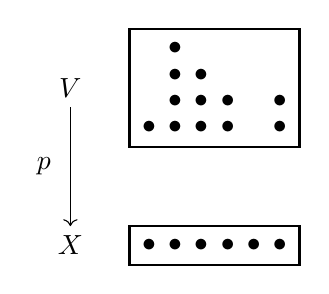
\begin{tikzpicture}
    \node (V) at (0,2) {$V$};
    \node (X) at (0,0) {$X$};
    \draw[->] (V) to node[label=left:{$p$}]{} (X);
    \draw[thick] (0.75,1.25) rectangle ++(2.16,1.5);
    \draw[thick] (0.75,-0.25) rectangle ++(2.16,0.5);
    \node at (1,1.5) {$\bullet$};
    \foreach \y in {1.5,1.83,2.16,2.5}
      \node at (1.33,\y) {$\bullet$};
    \foreach \y in {1.5,1.83,2.16}
      \node at (1.66,\y) {$\bullet$};
    \foreach \y in {1.5,1.83}
      \node at (2,\y) {$\bullet$};
    \foreach \y in {1.5,1.83}
      \node at (2.66,\y) {$\bullet$};
    \foreach \x in {1,1.33,1.66,2,2.33,2.66}
      \node at (\x,0) {$\bullet$};
  \end{tikzpicture}
\] I've drawn the elements of \(V\) and \(X\) as little circles, and
shown how each element in \(X\) has a bunch of elements of \(V\) sitting
over it. When degroupoidify this to get a vector in the vector space
\([X]\), we get: \[[V] = (1, 4, 3, 2, 0, 2)\] This vector is just a list
of numbers saying how many points of \(V\) are sitting over each point
of \(X\)!

Now we just need to generalize a bit further, to cover the case where
\(V\) is a groupoid: \[V \xrightarrow{p} X\] Sitting over each object
\(x\) in \(X\) we have its ``essential preimage'', which is a groupoid.
To get the vector \([V]\), we add up basis vectors \([x]\) in \([X]\),
one for each isomorphism class of objects in \(X\), multiplied by the
``cardinalities'' of their essential preimages.

Now you probably have two questions:

\begin{enumerate}
\def\labelenumi{\Alph{enumi})}
\tightlist
\item
  Given a functor \(p\colon V \to X\) between groupoids and an object
  \(x\) in \(X\), what's the ``essential preimage'' of \(x\)?
\end{enumerate}

and

\begin{enumerate}
\def\labelenumi{\Alph{enumi})}
\setcounter{enumi}{1}
\tightlist
\item
  what's the ``cardinality'' of a groupoid?
\end{enumerate}

Here are the answers:

\begin{enumerate}
\def\labelenumi{\Alph{enumi})}
\tightlist
\item
  An object in the essential preimage of \(x\) is an object \(v\) in
  \(V\) equipped with an isomorphism from \(p(v)\) to \(x\).
\end{enumerate}

(Exercise: define the morphisms in the essential preimage. Figure out
and prove the universal property of the essential preimage. Hint: the
essential preimage is a special case of a weak pullback!)

\begin{enumerate}
\def\labelenumi{\Alph{enumi})}
\setcounter{enumi}{1}
\tightlist
\item
  To compute the cardinality of a groupoid, we pick one object from each
  isomorphism class, count its automorphisms, take the \emph{reciprocal}
  of this number, and add these numbers up.
\end{enumerate}

(Exercise: check that the cardinality of the groupoid of finite sets is
\(e = 2.718281828\ldots\) If you get stuck, read
\protect\hyperlink{week147}{``Week 147''}.)

Also: define the morphisms in the essential preimage. Figure out and
prove the universal property of the essential preimage. Hint: the
essential preimage is a special case of a weak pullback!)

Okay. Now in principle you know how any groupoid over \(X\), say
\[V \to X\] determines a vector \([V]\) in \([X]\). You have to work
some examples to get a feel for it, but I want to get to the punchline.
We're unpeeling an onion here, and we're almost down to the core, where
you see there's nothing inside and wonder why you were crying so much.

So, let's finally figure out how a span of groupoids \[
  \begin{tikzcd}[column sep=tiny]
    &S\drar\dlar&
  \\X&&Y
  \end{tikzcd}
\] gives a linear operator \[[S]\colon [X] \to [Y]\] It's enough to know
what this operator does to vectors coming from groupoids over \(X\):
\[V \to X\] And, the trick is to notice that such a diagram is the same
as a silly span like this: \[
  \begin{tikzcd}[column sep=tiny]
    &V\drar\dlar&
  \\1&&X
  \end{tikzcd}
\] \(1\) is the groupoid with one object and one morphism, so there's
only one choice of the left leg here!

So here's what we do. To apply the operator \([S]\) coming from the span
\[
  \begin{tikzcd}[column sep=tiny]
    &S\drar\dlar&
  \\X&&Y
  \end{tikzcd}
\] to the vector \([V]\) corresponding to the silly span \[
  \begin{tikzcd}[column sep=tiny]
    &V\drar\dlar&
  \\1&&X
  \end{tikzcd}
\] we just compose these spans, and get a silly span \[
  \begin{tikzcd}[column sep=tiny]
    &SV\drar\dlar&
  \\1&&Y
  \end{tikzcd}
\] which picks out a vector \([SV]\) in \([Y]\). Then, we define
\[[S] [V] = [SV]\] Slick, eh? Of course you need to check that \([S]\)
is well-defined.

Given that, it's trivial to prove that \([-]\) gets along with
composition of spans: \[[TS] = [T] [S]\] At least, it's trivial once you
know that composition of spans is associative up to equivalence, and
equivalent spans give the same operator! But your friendly neighborhood
category theorist can check such facts in a jiffy, so let's just take
them for granted. Then the proof goes like this. We have: \[
  \begin{array}{rll}
    [TS][V] & = [(TS)V] & \text{by definition}
  \\& = [T(SV)] & \text{by those facts I just mentioned}
  \\& = [T][SV] & \text{by definition}
  \\& = [T][S][V] & \text{by definition}
  \end{array}
\] Since this is true for all \([V]\), we conclude \[[TS] = [T] [S]\]
Voilà!

By the way, if \protect\hyperlink{week47}{``Week 47''} doesn't satisfy
your hunger for information on groupoid cardinality, try this:

\begin{enumerate}
\def\labelenumi{\arabic{enumi})}
\setcounter{enumi}{18}
\tightlist
\item
  John Baez and James Dolan, ``From finite sets to Feynman diagrams'',
  in \emph{Mathematics Unlimited --- 2001 and Beyond}, vol.~\textbf{1},
  eds.~Bjorn Engquist and Wilfried Schmid, Springer, Berlin, 2001,
  pp.~29-50. Also available as
  \href{http://arxiv.org/abs/math.QA/0004133}{\texttt{math.QA/0004133}}.
\end{enumerate}

For more on turning spans of groupoids into linear operators, and
composing spans via weak pullback, try these:

\begin{enumerate}
\def\labelenumi{\arabic{enumi})}
\setcounter{enumi}{19}
\item
  Jeffrey Morton, ``Categorified algebra and quantum mechanics'',
  \emph{TAC} \textbf{16} (2006), 785--854. Available at
  \texttt{http://www.emis.de/journals/TAC/volumes/16/29/16-29abs.html};
  also available as
  \href{http://arxiv.org/abs/math.QA/0601458}{\texttt{math.QA/0601458}}.
\item
  Simon Byrne, \emph{On Groupoids and Stuff}, honors thesis, Macquarie
  University, 2005, available at
  \texttt{http://www.maths.mq.edu.au/\textasciitilde{}street/ByrneHons.pdf}
  and \texttt{http://math.ucr.edu/home/baez/qg-spring2004/ByrneHons.pdf}
\end{enumerate}

For a more leisurely exposition, with a big emphasis on applications to
combinatorics and the quantum mechanics of the harmonic oscillator, try:

\begin{enumerate}
\def\labelenumi{\arabic{enumi})}
\setcounter{enumi}{21}
\tightlist
\item
  John Baez and Derek Wise, ``Quantization and Categorification'',
  lecture notes available at:\\
  \texttt{http://math.ucr.edu/home/baez/qg-fall2003/}~\\
  \texttt{http://math.ucr.edu/home/baez/qg-winter2004/}~\\
  \texttt{http://math.ucr.edu/home/baez/qg-spring2004/}
\end{enumerate}

Finally, a technical note. Why did I say the degroupoidification process
was ``something like'' a functor? It's because spans of groupoids don't
want to be a category!

Already spans of sets don't naturally form a category. They form a weak
\(2\)-category! Since pullbacks are only defined up to canonical
isomorphism, composition of spans of sets is only associative up to
isomomorphism\ldots{} but luckily, this ``associator'' isomorphism
satisfies the ``pentagon identity'' and all that jazz, so we get a weak
\(2\)-category, or bicategory.

Similarly, spans of groupoids form a weak \(3\)-category. Weak pullbacks
are only defined up to canonical equivalence, so composition of spans of
groupoids are associative up to equivalence\ldots{} but luckily this
``associator'' equivalence satisfies the pentagon identity up to an
isomorphism, and this ``pentagonator'' isomomorphism satisfies a
coherence law of its own, governed by the 3d Stasheff polytope.

So, we're fairly high in the ladder of \(n\)-categories. But, if we want
a mere category, we can take groupoids and \emph{equivalence classes} of
spans. Then, degroupoidification gives a functor
\[[-]\colon [\text{finite groupoids}, \text{spans}] \to [\text{vector spaces}, \text{linear maps}]\]
That's the fact whose proof I tried to sketch here.

While I'm talking about annoying technicalities, note we need some sort
of finiteness assumption on our spans of groupoids to be sure all the
necessary sums converge. If we go all-out and restrict to spans where
all groupoids involved are finite, we'll be very safe. The cardinality
of a finite groupoid is a nonnegative rational number, so we can take
our vector spaces to be defined over the rational numbers.

But, it's also fun to consider ``tame'' groupoids, as defined that paper
I wrote with Jim Dolan. These have cardinalities that can be irrational
numbers, like \(e\). So, in this case we should use vector spaces over
the real numbers --- or complex numbers, but that's overkill.

Finding a class of groupoids or other entities whose cardinalities are
complex would be very nice, to push the whole groupoidification program
further into the complex world. In the above paper by Jeff Morton, he
uses sets over \(\mathrm{U}(1)\), but that's probably not the last word.

\begin{center}\rule{0.5\linewidth}{0.5pt}\end{center}

\begin{quote}
\emph{Viewed superficially, mathematics is the result of centuries of
effort by thousands of largely unconnected individuals scattered across
continents, centuries and millennia. However the internal logic of its
development much more closely resembles the work of a single intellect
developing its thought in a continuous and systematics way --- much as
in an orchestra playing a symphony written by some composer the theme
moves from one instrument to another, so that as soon as one performer
is forced to cut short his part, it is taken up by another player, who
continues with due attention to the score.}

--- I. R. Shavarevich
\end{quote}



\hypertarget{week257}{%
\section{October 14, 2007}\label{week257}}

Time flies! This week I'll finally finish saying what I did on my summer
vacation. After my trip to Oslo I stayed in London, or more precisely
Greenwich. While there, I talked with some good mathematicians and
physicists: in particular, Minhyong Kim, Ray Streater, Andreas Döring
and Chris Isham. I also went to a topology conference in
Sheffield\ldots{} and Eugenia Cheng explained some cool stuff on the
train ride there. I want to tell you about all this before I forget.

Also, the Tale of Groupoidification has taken a shocking new turn: it's
now becoming available as a series of \emph{videos}.

But first, some miscellaneous fun stuff on math and astronomy.

Math: if you haven't seen a sphere turn inside out, you've got to watch
this classic movie, now available for free online:

\begin{enumerate}
\def\labelenumi{\arabic{enumi})}
\tightlist
\item
  The Geometry Center, ``Outside in'',
  \texttt{http://video.google.com/videoplay?docid=-6626464599825291409}
\end{enumerate}

Astronomy: did you ever wonder where dust comes from? I'm not talking
about dust bunnies under your bed --- I'm talking about the dust
cluttering our galaxy, which eventually clumps together to form planets
and\ldots{} you and me!

These days most dust comes from aging stars called
\href{http://www.daviddarling.info/encyclopedia/A/AGB.html}{asymptotic
giant branch} stars:
\[\href{http://www.noao.edu/outreach/press/pr03/sb0307.html}{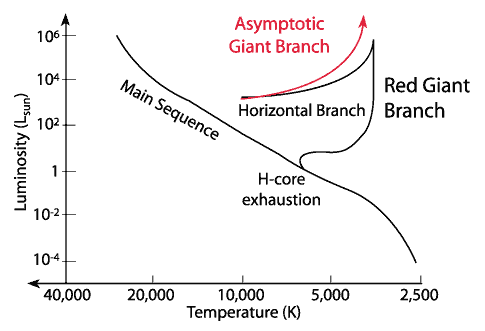
\includegraphics[max width=0.65\linewidth]{../images/asymptotic_giant_branch.png}}\]
The sun will eventually become one of these. The story goes like this:
first it'll keep burning until the hydrogen in its core is exhausted.
Then it'll cool and become a
\href{http://www.daviddarling.info/encyclopedia/R/redgiant.html}{red
giant}. Eventually
\href{http://www.daviddarling.info/encyclopedia/H/helium_flash.html}{helium
at the core will ignite}, and the Sun will heat up and
\href{http://www.daviddarling.info/encyclopedia/H/horizontal_branch.html}{shrink
again}\ldots{} but its core will then become cluttered with even heavier
elements, so it'll cool and expand once more, moving onto the
``asymptotic giant branch''. At this point it'll have a layered
structure: heavier elements near the bottom, then a layer of helium,
then hydrogen on the top:
\[\href{http://www.noao.edu/outreach/press/pr03/sb0307.html}{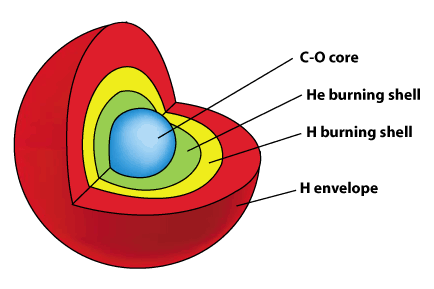
\includegraphics[max width=0.65\linewidth]{../images/asymptotic_giant_branch_cutaway.png}}\]
(A similar fate awaits any star between 0.6 and 10 solar masses, though
the details depend on the mass. For the more dramatic fate of heavier
stars, see \protect\hyperlink{week204}{``Week 204''}.)

Anyway: this layered structure is unstable, so asymptotic giant branch
stars pulse every 10 to 100 thousand years or so. And, they puff out
dust! Stellar wind then blows this dust out into space.

A great example is the Red Rectangle:
\[\href{http://apod.nasa.gov/apod/ap040513.html}{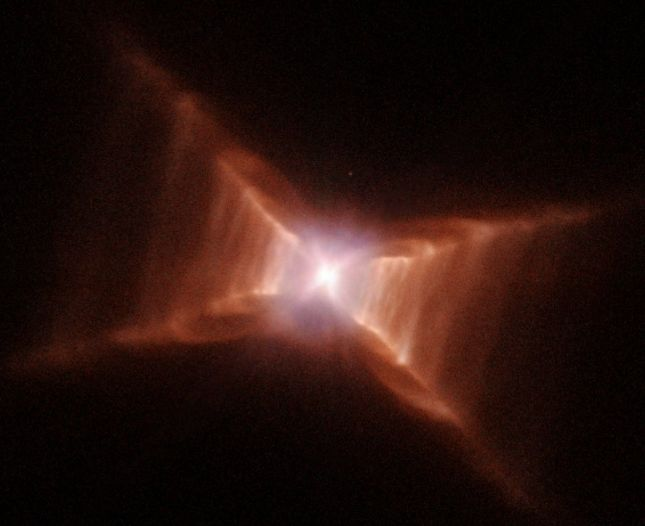
\includegraphics[max width=0.65\linewidth]{../images/red_rectangle.jpg}}\]

\begin{enumerate}
\def\labelenumi{\arabic{enumi})}
\setcounter{enumi}{1}
\tightlist
\item
  ``Rungs of the Red Rectangle'', Astronomy picture of the day, May 13,
  2004, \texttt{http://apod.nasa.gov/apod/ap040513.html}
\end{enumerate}

Here two stars 2300 light years from us are spinning around each other
while pumping out a huge torus of icy dust grains and hydrocarbon
molecules. It's not really shaped like a rectangle or X --- it just
looks that way. The scene is about 1/3 of a light year across.

Ciska Markwick-Kemper is an expert on dust. She's an astrophysicist at
the University of Manchester. Together with some coauthors, she wrote a
paper about the Red Rectangle:

\begin{enumerate}
\def\labelenumi{\arabic{enumi})}
\setcounter{enumi}{2}
\tightlist
\item
  F. Markwick-Kemper, J. D. Green, E. Peeters, ``Spitzer detections of
  new dust components in the outflow of the Red Rectangle'',
  \emph{Astrophys. J.} \textbf{628} (2005) L119--L122. Also available as
  \href{https://arxiv.org/abs/astro-ph/0506473}{\texttt{astro-ph/0506473}}.
\end{enumerate}

They used the Spitzer Space Telescope --- an infrared telescope on a
satellite in earth orbit --- to find evidence of magnesium and iron
oxides in this dust cloud.

But, what made dust in the early Universe? It took about a billion years
after the Big Bang for asymptotic giant branch stars to form. But we
know there was a lot of dust even before then! We can see it in distant
galaxies lit up by enormous black holes called ``quasars'', which pump
out vast amounts of radiation as stuff falls into them.

Markwick-Kemper and coauthors have also tackled that question:

\begin{enumerate}
\def\labelenumi{\arabic{enumi})}
\setcounter{enumi}{3}
\tightlist
\item
  F. Markwick-Kemper, S. C. Gallagher, D. C. Hines and J. Bouwman,
  ``Dust in the wind: crystalline silicates, corundum and periclase in
  PG 2112+059'', \emph{Astrophys. J.} \textbf{668} (2007), L107--L110.
  Also available as
  \href{https://arxiv.org/abs/0710.2225}{\texttt{arXiv:0710.2225}}.
\end{enumerate}

They used spectroscopy to identify various kinds of dust in a distant
galaxy: a magnesium silicate that geologists call ``forsterite'', a
magnesium oxide called ``periclase'', and aluminum oxide, otherwise
known as ``corundum'' --- you may have seen it on sandpaper.

And, they hypothesize that these dust grains were formed in the hot wind
emanating from the quasar at this galaxy's core!

So, besides being made of star dust, as in the Joni Mitchell song, you
also may contain a bit of black hole dust.

Okay --- now that we've got that settled, on to London!

Minhyong Kim is a friend I met back in 1986 when he was a grad student
at Yale. After dabbling in conformal field theory, he became a student
of Serge Lang and went into number theory. He recently moved to England
and started teaching at University College, London. I met him there this
summer, in front of the philosopher Jeremy Bentham, who had himself
mummified and stuck in a wooden cabinet near the school's entrance.

If you're not into number theory, maybe you should read this:

\begin{enumerate}
\def\labelenumi{\arabic{enumi})}
\setcounter{enumi}{4}
\tightlist
\item
  Minhyong Kim, ``Why everyone should know number theory'', available at
  \texttt{http://www.ucl.ac.uk/\textasciitilde{}ucahmki/numbers.pdf}
\end{enumerate}

Personally I never liked the subject until I realized it was a form of
\emph{geometry}. For example, when we take an equation like this
\[x^2 + y^3 = 1\] and look at the real solutions, we get a curve in the
plane --- a ``real curve''. If we look at the complex solutions, we get
something bigger. People call it a ``complex curve'', because it's
analogous to a real curve. But topologically, it's \(2\)-dimensional.

If we use polynomial equations with more variables, we get
higher-dimensional shapes called ``algebraic varieties'' --- either real
or complex. Either way, we can study these shapes using geometry and
topology.

But in number theory, we might study the solutions of these equations in
some other number system --- for example in \(\mathbb{Z}/p\), meaning
the integers modulo some prime \(p\). At first glance there's no
geometry involved anymore. After all, there's just a \emph{finite set}
of solutions! However, algebraic geometers have figured out how to apply
ideas from geometry and topology, mimicking tricks that work for the
real and complex numbers.

All this is very fun and mind-blowing --- especially when we reach
Grothendieck's idea of
\href{http://en.wikipedia.org/wiki/\%C3\%89tale_cohomology}{étale
topology}, developed around 1958. This is a way of studying ``holes'' in
things like algebraic varieties over finite fields. Amazingly, it gives
results that nicely match the results we get for the corresponding
complex algebraic varieties! That's part of what the
\href{http://en.wikipedia.org/wiki/Weil_conjectures}{Weil conjectures}
say.

You can learn the details here:

\begin{enumerate}
\def\labelenumi{\arabic{enumi})}
\setcounter{enumi}{5}
\tightlist
\item
  J. S. Milne, ``Lectures on Étale Cohomology'', available at
  \texttt{http://www.jmilne.org/math/CourseNotes/math732.html}
\end{enumerate}

Anyway, I quizzed about Minhyong about one of the big mysteries that's
been puzzling me lately. I want to know why the integers resemble a
3-dimensional space --- and how prime numbers give something like
``knots'' in this space!

I made a small step toward explaining this back in
\protect\hyperlink{week205}{``Week 205''}. There I sketched one of the
basic ideas of algebraic geometry: every commutative ring, for example
the integers or the integers modulo \(p\), has a kind of space
associated to it, called its ``spectrum''. We can think of elements of
the commutative ring as functions on this space. I also explained why
the process turning a commutative ring into a space is
``contravariant''. This implies that the obvious map from the integers
to the integers modulo \(p\) \[\mathbb{Z} \to \mathbb{Z}/p\] gives rise
to a map going \emph{the other way} between spectra:
\[\operatorname{Spec}(\mathbb{Z}/p) \to \operatorname{Spec}(\mathbb{Z})\]
In \protect\hyperlink{week218}{``Week 218''} I reviewed an old argument
saying that \(\operatorname{Spec}(\mathbb{Z})\) is analogous to the
complex plane, and that \(\operatorname{Spec}(\mathbb{Z}/p)\) is
analogous to a point. From this viewpoint, primes gives something like
points in a plane.

However, from a different viewpoint, primes give something like circles
in a 3d space!

The easy thing to see is how \(\operatorname{Spec}(\mathbb{Z}/p)\) acts
more like a circle than a point. In particular, its ``étale topology''
resembles the topology of a circle. Oversimplifying a bit, the reason is
that just as the circle has one \(n\)-fold cover for each integer
\(n > 0\), so too does \(\operatorname{Spec}(\mathbb{Z}/p)\). To get the
\(n\)-fold cover of the circle, you just wrap it around itself \(n\)
times. To get the \(n\)-fold cover of
\(\operatorname{Spec}(\mathbb{Z}/p)\), we take the spectrum of the field
with \(p^n\) elements, which is called \(\mathbb{F}_{p^n}\).
\(\mathbb{Z}/p\) sits inside this larger field:
\[\mathbb{Z}/p \to \mathbb{F}_{p^n}\] so by the contravariance I
mentioned, we get a map going the other way:
\[\operatorname{Spec}(\mathbb{F}_{p^n}) \to \operatorname{Spec}(\mathbb{Z}/p)\]
which is our \(n\)-fold cover.

I should explain this in much more detail someday --- it involves the
relation between étale cohomology, Galois theory and covering spaces. I
began tackling this in \protect\hyperlink{week213}{``Week 213''}, but I
have a long way to go.

Anyway, the basic idea here is that each prime \(p\) gives a ``circle''
\(\operatorname{Spec}(\mathbb{Z}/p)\) sitting inside
\(\operatorname{Spec}(\mathbb{Z})\). But the really nonobvious part is
that according to étale cohomology, \(\operatorname{Spec}(\mathbb{Z})\)
is \emph{\(3\)-dimensional} --- and the different circles corresponding
to different primes are \emph{linked!}

I've been fascinated by this ever since I heard about it, but I got even
more interested when I saw a draft of a paper by Kapranov and Smirnov. I
got it from Thomas Riepe, who got it from Yuri Manin. There's a version
on the web:

\begin{enumerate}
\def\labelenumi{\arabic{enumi})}
\setcounter{enumi}{6}
\tightlist
\item
  M. Kapranov and A. Smirnov, ``Cohomology determinants and reciprocity
  laws: number field case'', available at
  \texttt{http://wwwhomes.uni-bielefeld.de/triepe/F1.html}
\end{enumerate}

It begins:

\begin{quote}
The analogies between number fields and function fields have been a
long-time source of inspiration in arithmetic. However, one of the most
intriguing problems in this approach, namely the problem of the absolute
point, is still far from being satisfactorialy understood. The scheme
\(\operatorname{Spec}(\mathbb{Z})\), the final object in the category of
schemes, has dimension 1 with respect to the Zariski topology and at
least 3 with respect to the etale topology. This has generated a
long-standing desire to introduce a more mythical object \(P\), the
``absolute point'', with a natural morphism \(X \to P\) given for any
arithmetic scheme \(X\) {[}\ldots{]}
\end{quote}

Even though I don't fully understand this, I can tell something big is
afoot here. I think they're saying that because
\(\operatorname{Spec}(\mathbb{Z})\) is so big and fancy from the
viewpoint of étale topology, there should be some mysterious kind of
``point'' that's much smaller than \(\operatorname{Spec}(\mathbb{Z})\)
--- the ``absolute point''.

Anyway, in this paper the authors explain how the
\href{http://en.wikipedia.org/wiki/Legendre_symbol}{Legendre symbol} of
primes is analogous to the
\href{http://en.wikipedia.org/wiki/Linking_number}{linking number} of
knots.

The Legendre symbol depends on two primes: it's \(1\) or \(-1\)
depending on whether or not the first is a square modulo the second. The
linking number depends on two knots: it says how many times the first
winds around the second.

The linking number stays the same when you switch the two knots. The
Legendre symbol has a subtler symmetry when you switch the two primes:
this symmetry is called
\href{http://golem.ph.utexas.edu/category/2007/06/quadratic_reciprocity.html}{quadratic
reciprocity}, and it has lots of proofs, starting with a bunch by Gauss
--- all a bit tricky.

I'd feel very happy if I truly understood why quadratic reciprocity
reduces to the symmetry of the linking number when we think of primes as
analogous to knots. Unfortunately, I'll need to think a lot more before
I really get the idea. I got into number theory late in life, so I'm
pretty slow at it.

This paper studies subtler ways in which primes can be ``linked'':

\begin{enumerate}
\def\labelenumi{\arabic{enumi})}
\setcounter{enumi}{7}
\tightlist
\item
  Masanori Morishita, ``Milnor invariants and Massey products for prime
  numbers'', \emph{Compositio Mathematica} \textbf{140} (2004), 69--83.
\end{enumerate}

You may know the
\href{http://en.wikipedia.org/wiki/Borromean_rings}{Borromean rings}, a
design where no two rings are linked in isolation, but all three are
when taken together. Here the linking numbers are zero, but the linking
can be detected by something called the ``Massey triple product''.
Morishita generalizes this to primes!

But I want to understand the basics\ldots{}

The secret \(3\)-dimensional nature of the integers and certain other
``rings of algebraic integers'' seems to go back at least to the work of
Artin and Verdier:

\begin{enumerate}
\def\labelenumi{\arabic{enumi})}
\setcounter{enumi}{8}
\tightlist
\item
  Michael Artin and Jean-Louis Verdier, \emph{Seminar on étale
  cohomology of number fields}, Woods Hole, 1964.
\end{enumerate}

You can see it clearly here, starting in section 2:

\begin{enumerate}
\def\labelenumi{\arabic{enumi})}
\setcounter{enumi}{9}
\tightlist
\item
  Barry Mazur, ``Notes on the étale cohomology of number fields'',
  \emph{Annales Scientifiques de l'Ecole Normale Superieure Ser. 4}
  \textbf{6} (1973), 521--552. Also available at
  \texttt{http://www.numdam.org/numdam-bin/fitem?id=ASENS\_1973\_4\_6\_4\_521\_0}
\end{enumerate}

By now, a big ``dictionary'' relating knots to primes has been developed
by Kapranov, Mazur, Morishita, and Reznikov. This seems like a readable
introduction:

\begin{enumerate}
\def\labelenumi{\arabic{enumi})}
\setcounter{enumi}{10}
\tightlist
\item
  Adam S. Sikora, ``Analogies between group actions on \(3\)-manifolds
  and number fields'', available as
  \href{http://arxiv.org/abs/math/0107210}{\texttt{arXiv:math/0107210}}.
\end{enumerate}

I need to study it. These might also be good --- I haven't looked at
them yet:

\begin{enumerate}
\def\labelenumi{\arabic{enumi})}
\setcounter{enumi}{11}
\item
  Masanori Morishita, ``On certain analogies between knots and primes'',
  \emph{J. Reine Angew. Math.} \textbf{550} (2002), 141--167.

  Masanori Morishita, ``On analogies between knots and primes'',
  \emph{Sugaku} \textbf{58} (2006), 40--63.
\end{enumerate}

After giving a talk on \(2\)-Hilbert spaces at University College, I
went to dinner with Minhyong and some folks including Ray Streater. Ray
Streater and Arthur Wightman wrote the book ``PCT, Spin, Statistics and
All That''. Like almost every mathematician who has seriously tried to
understand quantum field theory, I've learned a lot from this book. So,
it was fun meeting Streater, talking with him --- and finding out he'd
once been made an honorary colonel of the US Army to get a free plane
trip to the Rochester Conference! This was a big important particle
physics conference, back in the good old days.

He also described Geoffrey Chew's Rochester conference talk on the
analytic S-matrix, given at the height of the
\href{http://en.wikipedia.org/wiki/Bootstrap_model}{bootstrap model}
fad. Wightman asked Chew: why assume from the start that the S-matrix
was analytic? Why not try to derive it from simpler principles? Chew
replied that ``everything in physics is smooth''. Wightman asked about
smooth functions that aren't analytic. Chew thought a moment and replied
that there weren't any.

Ha-ha-ha\ldots{}

What's the joke? Well, first of all, Wightman had already succeeded in
deriving the analyticity of the S-matrix from simpler principles.
Second, any good mathematician --- but not necessarily every physicist,
like Chew --- will know examples of smooth functions that aren't
analytic.

Anyway, Streater has just finished an interesting book on ``lost
causes'' in physics: ideas that sounded good, but never panned out. Of
course it's hard to know when a cause is truly lost. But a good
pragmatic definition of a lost cause in physics is a topic that
shouldn't be given as a thesis problem.

So, if you're a physics grad student and some professor wants you to
work on hidden variable theories, or octonionic quantum mechanics, or
deriving laws of physics from Fisher information, you'd better read
this:

\begin{enumerate}
\def\labelenumi{\arabic{enumi})}
\setcounter{enumi}{12}
\tightlist
\item
  Ray F. Streater, \emph{Lost Causes in and Beyond Physics}, Springer
  Verlag, Berlin, 2007.
\end{enumerate}

(I like octonions --- but I agree with Streater about not inflicting
them on physics grad students! Even though all my students are in the
math department, I still wouldn't want them working \emph{mainly} on
something like that. There's a lot of more general, clearly useful stuff
that students should learn.)

I also spoke to Andreas Döring and Chris Isham about their work on topos
theory and quantum physics. Andreas Döring lives near Greenwich, while
Isham lives across the Thames in London proper. So, I talked to Döring a
couple times, and once we visited Isham at his house.

I mainly mention this because Isham is one of the gurus of quantum
gravity, profoundly interested in philosophy\ldots{} so I was surprised,
at the end of our talk, when he showed me into a room with a huge rack
of computers hooked up to a bank of about 8 video monitors, and controls
reminiscent of an airplane cockpit.

It turned out to be his homemade flight simulator! He's been a hobbyist
electrical engineer for years --- the kind of guy who loves nothing more
than a soldering iron in his hand. He'd just gotten a big 750-watt power
supply, since he'd blown out his previous one.

Anyway, he and Döring have just come out with a series of papers:

\begin{enumerate}
\def\labelenumi{\arabic{enumi})}
\setcounter{enumi}{13}
\item
  Andreas Döring and Christopher Isham, ``A topos foundation for
  theories of physics: I. Formal languages for physics'', available as
  \href{https://arxiv.org/abs/quant-ph/0703060}{\texttt{quant-ph/0703060}}.

  ``II. Daseinisation and the liberation of quantum theory'', available
  as
  \href{https://arxiv.org/abs/quant-ph/0703062}{\texttt{quant-ph/0703062}}.

  ``III. The representation of physical quantities with arrows'',
  available as
  \href{https://arxiv.org/abs/quant-ph/0703064}{\texttt{quant-ph/0703064}}.

  ``IV. Categories of systems'', available as
  \href{https://arxiv.org/abs/quant-ph/0703066}{\texttt{quant-ph/0703066}}.
\end{enumerate}

Though they probably don't think of it this way, you can think of their
work as making precise Bohr's ideas on seeing the quantum world through
classical eyes. Instead of talking about all observables at once, they
consider collections of observables that you can measure simultaneously
without the uncertainty principle kicking in. These collections are
called ``commutative subalgebras''.

You can think of a commutative subalgebra as a classical snapshot of the
full quantum reality. Each snapshot only shows part of the reality. One
might show an electron's position; another might show it's momentum.

Some commutative subalgebras contain others, just like some open sets of
a topological space contain others. The analogy is a good one, except
there's no one commutative subalgebra that contains \emph{all} the
others.

Topos theory is a kind of ``local'' version of logic, but where the
concept of locality goes way beyond the ordinary notion from topology.
In topology, we say a property makes sense ``locally'' if it makes sense
for points in some particular open set. In the Döring-Isham setup, a
property makes sense ``locally'' if it makes sense ``within a particular
classical snapshot of reality'' --- that is, relative to a particular
commutative subalgebra.

(Speaking of topology and its generalizations, this work on topoi and
physics is related to the ``étale topology'' idea I mentioned a while
back --- but technically it's much simpler. The
\href{http://en.wikipedia.org/wiki/Grothendieck_topology}{étale
topology} lets you define a topos of
\href{http://en.wikipedia.org/wiki/Grothendieck_topology\#Sites_and_sheaves}{sheaves}
on a certain category. The Döring-Isham work just uses the topos of
\href{http://en.wikipedia.org/wiki/Presheaf_(category_theory)}{presheaves}
on the poset of commutative subalgebras. Trust me --- while this may
sound scary, it's much easier.)

Döring and Isham set up a whole program for doing physics ``within a
topos'', based on existing ideas on how to do math in a topos. You can
do vast amounts of math inside any topos just as if you were in the
ordinary world of set theory --- but using intuitionistic logic instead
of classical logic. Intuitionistic logic denies the principle of
excluded middle, namely:

\begin{quote}
``For any statement \(P\), either \(P\) is true or
\(\operatorname{not}(P)\) is true.''
\end{quote}

In Döring and Isham's setup, if you pick a commutative subalgebra that
contains the position of an electron as one of its observables, it can't
contain the electron's momentum. That's because these observables don't
commute: you can't measure them both simultaneously. So, working
``locally'' --- that is, relative to this particular subalgebra --- the
statement \[P = \mbox{"the momentum of the electron is zero"}\] is
neither true nor false! It's just not defined.

Their work has inspired this very nice paper:

\begin{enumerate}
\def\labelenumi{\arabic{enumi})}
\setcounter{enumi}{14}
\tightlist
\item
  Chris Heunen and Bas Spitters, ``A topos for algebraic quantum
  theory'', available as
  \href{http://arxiv.org/abs/0709.4364}{\texttt{arXiv:0709.4364.}}
\end{enumerate}

so let me explain that too.

I said you can do a lot of math inside a topos. In particular, you can
define an algebra of observables --- or technically, a
``\(C^*\)-algebra''.

By the Isham-Döring work I just sketched, any \(C^*\)-algebra of
observables gives a topos. Heunen and Spitters show that the original
\(C^*\)-algebra gives rise to a \(C^*\)-algebra \emph{in this topos},
which is \emph{commutative} even if the original one was noncommutative!
That actually makes sense, since in this setup each ``local view'' of
the full quantum reality is classical.

So, they get this sort of picture:
\[\href{http://arxiv.org/abs/0709.4364}{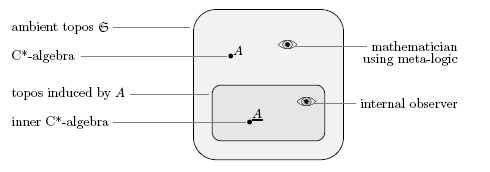
\includegraphics[max width=0.65\linewidth]{../images/heunen_spitters.jpg}}\]
I've been taking the ``ambient topos'' to be the familiar category of
sets, but it could be something else.

What's really neat is that the Gelfand-Naimark theorem, saying
commutative \(C^*\)-algebras are always algebras of continuous functions
on compact Hausdorff spaces, can be generalized to work within any
topos. So, we get a space \emph{in our topos} such that observables of
the \(C^*\)-algebra \emph{in the topos} are just functions on this
space.

I know this sounds technical if you're not into this stuff. But it's
really quite wonderful. It basically means this: using topos logic, we
can talk about a classical space of states for a quantum system!
However, this space typically has ``no global points'' --- that's called
the ``Kochen-Specker theorem''. In other words, there's no overall
classical reality that matches all the classical snapshots.

As you can probably tell, category theory is gradually seeping into this
post, though I've been doing my best to keep it hidden. Now I want to
say what Eugenia Cheng explained on that train to Sheffield. But at this
point, I'll break down and assume you know some category theory --- for
example, monads.

If you don't know about monads, never fear! I defined them in
\protect\hyperlink{week89}{``Week 89''}, and studied them using string
diagrams in \protect\hyperlink{week92}{``Week 92''}. Even better,
Eugenia Cheng and Simon Willerton have formed a little group called the
Catsters --- and under this name, they've put some videos about monads
and string diagrams onto YouTube! This is a really great new use of
technology. So, you should also watch these:

\begin{enumerate}
\def\labelenumi{\arabic{enumi})}
\setcounter{enumi}{15}
\item
  The Catsters, ``Monads'',
  \texttt{http://youtube.com/view\_play\_list?p=0E91279846EC843E}

  The Catsters, ``Adjunctions'',
  \texttt{http://youtube.com/view\_play\_list?p=54B49729E5102248}

  The Catsters, ``String diagrams, monads and adjunctions'',
  \texttt{http://youtube.com/view\_play\_list?p=50ABC4792BD0A086}
\end{enumerate}

A very famous monad is the ``free abelian group'' monad
\[F\colon \mathsf{Set} \to \mathsf{Set}\] which eats any set \(X\) and
spits out the free abelian group on \(X\), say \$F(X)\$4. A guy in
\(F(X)\) is just a formal linear combination of guys in \(X\), with
integer coefficients.

Another famous monad is the ``free monoid'' monad
\[G\colon \mathsf{Set} \to \mathsf{Set}\] This eats any set \(X\) and
spits out the free monoid on \(X\), namely \(G(X)\). A guy in \(G(X)\)
is just a formal product of guys in \(X\).

Now, there's yet another famous monad, called the ``free ring'' monad,
which eats any set \(X\) and spits out the free ring on this set. But,
it's easy to see that this is just \(F(G(X))\)! After all, \(F(G(X))\)
consists of formal linear combinations of formal products of guys in
\(X\). But that's precisely what you find in the free ring on \(X\).

But why is \(FG\) a monad? There's more to a monad than just a functor.
A monad is really a kind of \emph{monoid} in the world of functors from
our category (here \(\mathsf{Set}\)) to itself. In particular, since
\(F\) is a monad, it comes with a natural transformation called a
``multiplication'': \[m\colon FF \Rightarrow F\] which sends formal
linear combinations of formal linear combinations to formal linear
combinations, in the obvious way. Similarly, since \(G\) is a monad, it
comes with a natural transformation \[n\colon GG \Rightarrow G\] sending
formal products of formal products to formal products. But how does
\(FG\) get to be a monad? For this, we need some natural transformation
from \(FGFG\) to \(FG\)!

There's an obvious thing to try, namely
\[FGFG \Rightarrow FFGG \xRightarrow{mn} FG\] where in the first step we
switch \(G\) and \(F\) somehow, and in the second step we use \(m\) and
\(n\). But, how do we do the first step?

We need a natural transformation \[d\colon GF \Rightarrow FG\] which
sends formal products of formal linear combinations to formal linear
combinations of formal products. Such a thing obviously exists; for
example, it sends \[(x + 2y)(x - 3z)\] to \[xx + 2yx - 3xz - 6yz\] It's
just the distributive law!

Quite generally, to make the composite of monads \(F\) and \(G\) into a
new monad \(FG\), we need something that people call a ``distributive
law'', which is a natural transformation \[d\colon GF \Rightarrow FG\]
This must satisfy some equations --- but you can work out those
yourself. For example, you can demand that
\[FGFG \xRightarrow{FdG} FFGG \xRightarrow{mn} FG\] make \(FG\) into a
monad, and see what that requires. (Besides the ``multiplication'' in
our monad, we also need the ``unit'', so you should also think about
that --- I'm ignoring it here because it's less sexy than the
multiplication, but it's equally essential.)

However: all this becomes more fun with string diagrams! As the Catsters
explain, and I explained in \protect\hyperlink{week89}{``Week 89''}, the
multiplication \(m\colon FF \Rightarrow F\) can be drawn like this: \[
  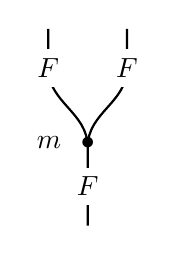
\begin{tikzpicture}
    \begin{knot}
      \strand[thick] (0,0.5)
        to (0,0)
        to [out=down,in=up] (0.5,-1)
        to (0.5,-2);
      \strand[thick] (1,0.5)
        to (1,0)
        to [out=down,in=up] (0.5,-1);
    \end{knot}
    \node[fill=white] at (0,0) {$F$};
    \node[fill=white] at (1,0) {$F$};
    \node[label=left:{$m$}] at (0.5,-0.95) {$\bullet$};
    \node[fill=white] at (0.5,-1.5) {$F$};
  \end{tikzpicture}
\] And, it has to satisfy the associative law, which says we get the
same answer either way when we multiply three things: \[
  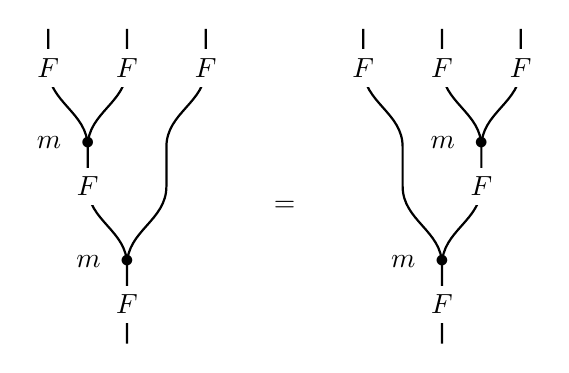
\begin{tikzpicture}
    \begin{knot}
      \strand[thick] (0,0.5)
        to (0,0)
        to [out=down,in=up] (0.5,-1)
        to (0.5,-1.5)
        to [out=down,in=up] (1,-2.5)
        to (1,-3.5);
      \strand[thick] (1,0.5)
        to (1,0)
        to [out=down,in=up] (0.5,-1);
      \strand[thick] (2,0.5)
        to (2,0)
        to [out=down,in=up] (1.5,-1)
        to (1.5,-1.5)
        to [out=down,in=up] (1,-2.5);
    \end{knot}
    \node[fill=white] at (0,0) {$F$};
    \node[fill=white] at (1,0) {$F$};
    \node[fill=white] at (2,0) {$F$};
    \node[label=left:{$m$}] at (0.5,-0.95) {$\bullet$};
    \node[label=left:{$m$}] at (1,-2.45) {$\bullet$};
    \node[fill=white] at (0.5,-1.5) {$F$};
    \node[fill=white] at (1,-3) {$F$};
    \node at (3,-1.75) {$=$};
    \begin{scope}[xscale=-1,shift={(-6,0)}]
    \begin{knot}
      \strand[thick] (0,0.5)
        to (0,0)
        to [out=down,in=up] (0.5,-1)
        to (0.5,-1.5)
        to [out=down,in=up] (1,-2.5)
        to (1,-3.5);
      \strand[thick] (1,0.5)
        to (1,0)
        to [out=down,in=up] (0.5,-1);
      \strand[thick] (2,0.5)
        to (2,0)
        to [out=down,in=up] (1.5,-1)
        to (1.5,-1.5)
        to [out=down,in=up] (1,-2.5);
    \end{knot}
    \node[fill=white] at (0,0) {$F$};
    \node[fill=white] at (1,0) {$F$};
    \node[fill=white] at (2,0) {$F$};
    \node[label=left:{$m$}] at (0.5,-0.95) {$\bullet$};
    \node[label=left:{$m$}] at (1,-2.45) {$\bullet$};
    \node[fill=white] at (0.5,-1.5) {$F$};
    \node[fill=white] at (1,-3) {$F$};
    \end{scope}
  \end{tikzpicture}
\] The multiplication \(n\colon GG \Rightarrow G\) looks similar to
\(m\), and it too has to satisfy the associative law.

How do we draw the distributive law \(d\colon FG \Rightarrow GF\)? Since
it's a process of switching two things, we draw it as a \emph{braiding}:
\[
  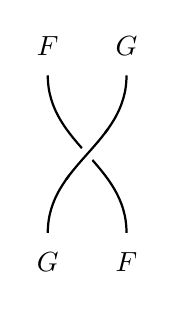
\begin{tikzpicture}
    \node[label=above:{$F$}] at (0,0) {};
    \node[label=above:{$G$}] at (1,0) {};
    \begin{knot}[clip width=7]
      \strand[thick] (1,0)
        to [out=down,in=up] (0,-2);
      \strand[thick] (0,0)
        to [out=down,in=up] (1,-2);
    \end{knot}
    \node[label=below:{$G$}] at (0,-2) {};
    \node[label=below:{$F$}] at (1,-2) {};
  \end{tikzpicture}
\] I hope you see how incredibly cool this is: the good old distributive
law is now a \emph{braiding}, which pushes our diagrams into the third
dimension!

Given this, let's draw the multiplication for our would-be monad \(FG\),
namely \[FGFG \xRightarrow{FdG} FFGG \xRightarrow{mn} FG\] It looks like
this: \[
  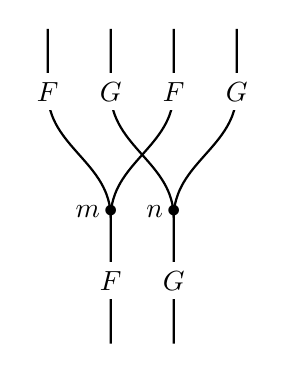
\begin{tikzpicture}[scale=1.6]
    \begin{scope}
      \begin{knot}
        \strand[thick] (0,0.5)
          to (0,0)
          to [out=down,in=up] (0.5,-1)
          to (0.5,-2);
        \strand[thick] (1,0.5)
          to (1,0)
          to [out=down,in=up] (0.5,-1);
      \end{knot}
      \node[fill=white] at (0,0) {$F$};
      \node[fill=white] at (1,0) {$F$};
      \node[label={[label distance=-2mm]left:{$m$}}] at (0.5,-0.95) {$\bullet$};
      \node[fill=white] at (0.5,-1.5) {$F$};
    \end{scope}
    \begin{scope}[shift={(0.5,0)}]
      \begin{knot}
        \strand[thick] (0,0.5)
          to (0,0)
          to [out=down,in=up] (0.5,-1)
          to (0.5,-2);
        \strand[thick] (1,0.5)
          to (1,0)
          to [out=down,in=up] (0.5,-1);
      \end{knot}
      \node[fill=white] at (0,0) {$G$};
      \node[fill=white] at (1,0) {$G$};
      \node[label={[label distance=-2mm]left:{$n$}}] at (0.5,-0.95) {$\bullet$};
      \node[fill=white] at (0.5,-1.5) {$G$};
    \end{scope}
  \end{tikzpicture}
\] Now, we want \emph{this} multiplication to be associative! So, we
need to draw an equation like this: \[
  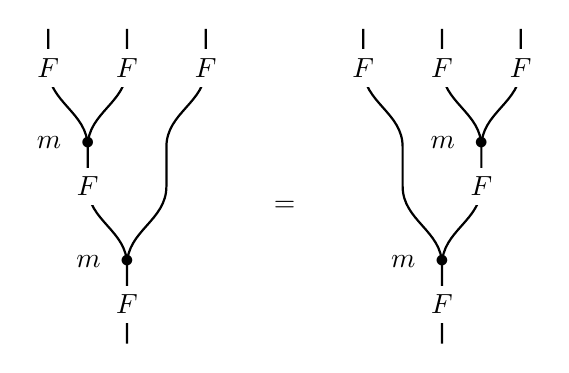
\begin{tikzpicture}
    \begin{knot}
      \strand[thick] (0,0.5)
        to (0,0)
        to [out=down,in=up] (0.5,-1)
        to (0.5,-1.5)
        to [out=down,in=up] (1,-2.5)
        to (1,-3.5);
      \strand[thick] (1,0.5)
        to (1,0)
        to [out=down,in=up] (0.5,-1);
      \strand[thick] (2,0.5)
        to (2,0)
        to [out=down,in=up] (1.5,-1)
        to (1.5,-1.5)
        to [out=down,in=up] (1,-2.5);
    \end{knot}
    \node[fill=white] at (0,0) {$F$};
    \node[fill=white] at (1,0) {$F$};
    \node[fill=white] at (2,0) {$F$};
    \node[label=left:{$m$}] at (0.5,-0.95) {$\bullet$};
    \node[label=left:{$m$}] at (1,-2.45) {$\bullet$};
    \node[fill=white] at (0.5,-1.5) {$F$};
    \node[fill=white] at (1,-3) {$F$};
    \node at (3,-1.75) {$=$};
    \begin{scope}[xscale=-1,shift={(-6,0)}]
      \begin{knot}
        \strand[thick] (0,0.5)
          to (0,0)
          to [out=down,in=up] (0.5,-1)
          to (0.5,-1.5)
          to [out=down,in=up] (1,-2.5)
          to (1,-3.5);
        \strand[thick] (1,0.5)
          to (1,0)
          to [out=down,in=up] (0.5,-1);
        \strand[thick] (2,0.5)
          to (2,0)
          to [out=down,in=up] (1.5,-1)
          to (1.5,-1.5)
          to [out=down,in=up] (1,-2.5);
      \end{knot}
      \node[fill=white] at (0,0) {$F$};
      \node[fill=white] at (1,0) {$F$};
      \node[fill=white] at (2,0) {$F$};
      \node[label=left:{$m$}] at (0.5,-0.95) {$\bullet$};
      \node[label=left:{$m$}] at (1,-2.45) {$\bullet$};
      \node[fill=white] at (0.5,-1.5) {$F$};
      \node[fill=white] at (1,-3) {$F$};
    \end{scope}
  \end{tikzpicture}
\] but with the strands \emph{doubled}, as above --- I'm too lazy to
draw this here. And then we need to find some nice conditions that make
this associative law true. Clearly we should use the associative laws
for \(m\) and \(n\), but the ``braiding'' --- the distributive law
\(d\colon FG \Rightarrow GF\) --- also gets into the act.

I'll leave this as a pleasant exercise in string diagram manipulation.
If you get stuck, you can peek in the back of the book:

\begin{enumerate}
\def\labelenumi{\arabic{enumi})}
\setcounter{enumi}{16}
\tightlist
\item
  Wikipedia, ``Distibutive law between monads'',
  \texttt{http://en.wikipedia.org/wiki/Distributive\_law\_between\_monads}
\end{enumerate}

The two scary commutative rectangles on this page are the ``nice
conditions'' you need. They look nicer as string diagrams. One looks
like this: \[
  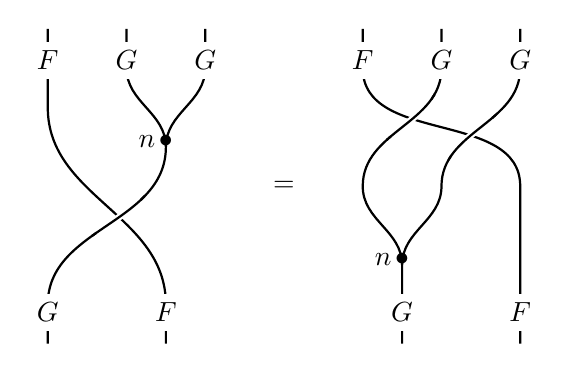
\begin{tikzpicture}
    \begin{knot}
      \strand[thick] (1,0)
        to (1,-0.5)
        to [out=down,in=up] (1.5,-1.5)
        to [out=down,in=up] (0,-3.5)
        to (0,-4);
      \strand[thick] (2,0)
        to (2,-0.5)
        to [out=down,in=up] (1.5,-1.5);
      \strand[thick] (0,0)
        to (0,-1)
        to [out=down,in=up] (1.5,-3.5)
        to (1.5,-4);
    \end{knot}
    \node[fill=white] at (0,-0.4) {$F$};
    \node[fill=white] at (1,-0.4) {$G$};
    \node[fill=white] at (2,-0.4) {$G$};
    \node[fill=white] at (0,-3.6) {$G$};
    \node[fill=white] at (1.5,-3.6) {$F$};
    \node[label={[label distance=-2mm]left:{$n$}}] at (1.5,-1.43) {$\bullet$};
    \node at (3,-2) {$=$};
    \begin{scope}[shift={(4,0)}]
      \begin{knot}
        \strand[thick] (1,0)
          to (1,-0.5)
          to [out=down,in=up] (0,-2)
          to [out=down,in=up] (0.5,-3)
          to (0.5,-4);
        \strand[thick] (2,0)
          to (2,-0.5)
          to [out=down,in=up] (1,-2)
          to [out=down,in=up] (0.5,-3);
        \strand[thick] (0,0)
          to (0,-0.5)
          to [out=down,in=up] (2,-2)
          to (2,-4);
      \end{knot}
      \node[fill=white] at (0,-0.4) {$F$};
      \node[fill=white] at (1,-0.4) {$G$};
      \node[fill=white] at (2,-0.4) {$G$};
      \node[fill=white] at (0.5,-3.6) {$G$};
      \node[fill=white] at (2,-3.6) {$F$};
    \node[label={[label distance=-2mm]left:{$n$}}] at (0.5,-2.93) {$\bullet$};
    \end{scope}
  \end{tikzpicture}
\]

\begin{verbatim}
         F\    G\   /G             F\    G/    /G
           \     \ /                 \   /    /
            \     |n                  \ /    /
             \   /                     /    /
              \ /             =       / \  /
               /                     /    /
              / \                   /    /  
             /   \                  \   /  \
            /     \                  \ /    \
          G/       \F                 |n     \F
          /         \                G|       \
\end{verbatim}

In words:

\begin{quote}
``multiply two \(G\)'s and slide the result over an \(F\)'' =\\
``slide both the \(G\)'s over the \(F\) and then multiply them''
\end{quote}

If the pictures were made of actual string, this would be obvious!

The other condition is very similar. I'm too lazy to draw it, but it
says

\begin{quote}
``multiply two \(F\)'s and slide the result under a \(G\)'' =\\
``slide both the \(F\)'s under a \(G\) and then multiply them''
\end{quote}

All this is very nice, and it goes back to a paper by Beck:

\begin{enumerate}
\def\labelenumi{\arabic{enumi})}
\setcounter{enumi}{17}
\tightlist
\item
  Jon Beck, \emph{Distributive laws}, Lecture Notes in Mathematics
  \textbf{80}, Springer, Berlin, 1969, pp.~119--140.
\end{enumerate}

This isn't what Eugenia explained to me, though --- I already knew this
stuff. She started out by explaining something in a paper by Street:

\begin{enumerate}
\def\labelenumi{\arabic{enumi})}
\setcounter{enumi}{18}
\tightlist
\item
  Ross Street, ``The formal theory of monads'', \emph{J. Pure Appl.
  Alg.} \textbf{2} (1972), 149--168.
\end{enumerate}

which is reviewed at the beginning here:

\begin{enumerate}
\def\labelenumi{\arabic{enumi})}
\setcounter{enumi}{19}
\tightlist
\item
  Steve Lack and Ross Street, ``The formal theory of monads II'',
  \emph{J. Pure Appl. Alg.} \textbf{175} (2002), 243--265. Also
  available at
  \texttt{http://www.maths.usyd.edu.au/u/stevel/papers/ftm2.html}
\end{enumerate}

(Check out the cool string diagrams near the end!)

Street noted that we can talk about monads, not just in the
\(2\)-category of categories, but in any \(2\)-category. I actually
explained monads at this level of generality back in
\protect\hyperlink{week89}{``Week 89''}. Indeed, for any \(2\)-category
\(\mathcal{C}\), there's a \(2\)-category \(\mathsf{Mnd}(\mathcal{C})\)
of monads in \(\mathcal{C}\).

And, he noted that a monad in \(\mathsf{Mnd}(\mathcal{C})\) is a pair of
monads in \(\mathcal{C}\) related by a distributive law!

That's already mindbogglingly beautiful. According to Eugenia, it's
practically the last sentence in Street's paper. But in her new work:

\begin{enumerate}
\def\labelenumi{\arabic{enumi})}
\setcounter{enumi}{20}
\tightlist
\item
  Eugenia Cheng, ``Iterated distributive laws'', available as
  \href{http://arxiv.org/abs/0710.1120}{\texttt{arXiv:0710.1120}}.
\end{enumerate}

she goes a bit further: she considers monads in
\(\mathsf{Mnd}(\mathsf{Mnd}(C))\), and so on. Here's the punchline, at
least for today: she shows that a monad in
\(\mathsf{Mnd}(\mathsf{Mnd}(C))\) is a triple of monads \(F, G, H\)
related by distributive laws satisfying the Yang-Baxter equation: \[
  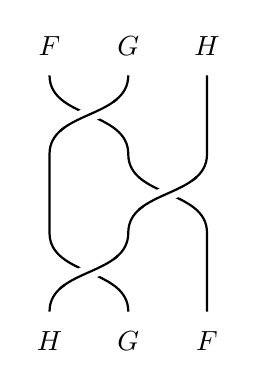
\begin{tikzpicture}
    \node[label=above:{$F$}] at (0,0) {};
    \node[label=above:{$G$}] at (1,0) {};
    \node[label=above:{$H$}] at (2,0) {};
    \begin{knot}[clip width=7]
      \strand[thick] (0,0)
        to [out=down,in=up] (1,-1)
        to [out=down,in=up] (2,-2)
        to (2,-3);
      \strand[thick] (1,0)
        to [out=down,in=up] (0,-1)
        to (0,-2)
        to [out=down,in=up] (1,-3);
      \strand[thick] (2,0)
        to (2,-1)
        to [out=down,in=up] (1,-2)
        to [out=down,in=up] (0,-3);
      \flipcrossings{1,2,3};
    \end{knot}
    \node[label=below:{$H$}] at (0,-3) {};
    \node[label=below:{$G$}] at (1,-3) {};
    \node[label=below:{$F$}] at (2,-3) {};
  \end{tikzpicture}
  \raisebox{4em}{\quad=\quad}
  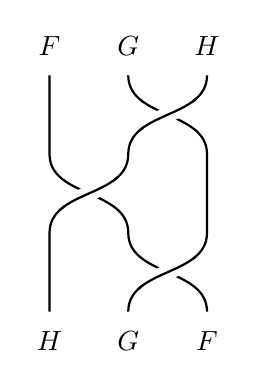
\begin{tikzpicture}
    \node[label=above:{$F$}] at (0,0) {};
    \node[label=above:{$G$}] at (1,0) {};
    \node[label=above:{$H$}] at (2,0) {};
    \begin{knot}[clip width=7]
      \strand[thick] (0,0)
        to (0,-1)
        to [out=down,in=up] (1,-2)
        to [out=down,in=up] (2,-3);
      \strand[thick] (1,0)
        to [out=down,in=up] (2,-1)
        to (2,-2)
        to [out=down,in=up] (1,-3);
      \strand[thick] (2,0)
        to [out=down,in=up] (1,-1)
        to [out=down,in=up] (0,-2)
        to (0,-3);
      \flipcrossings{1,2,3};
    \end{knot}
    \node[label=below:{$H$}] at (0,-3) {};
    \node[label=below:{$G$}] at (1,-3) {};
    \node[label=below:{$F$}] at (2,-3) {};
  \end{tikzpicture}
\] This is also just what you need to make the composite \(FGH\) into a
monad!

By the way, the pathetic piece of ASCII art above is lifted from
\protect\hyperlink{week1}{``Week 1''}, where I first explained the
Yang-Baxter equation. That was back in 1993. So, it's only taken me 14
years to learn that you can derive this equation from considering monads
in the category of monads in the category of monads in a \(2\)-category.

You may wonder if this counts as progress --- but Eugenia studies lots
of \emph{examples} of this sort of thing, so it's far from pointless.

Okay\ldots{} finally, the Tale of Groupoidification. I'm a bit tired
now, so instead of telling you more of the tale, let me just say the big
news.

Starting this fall, James Dolan and I are running a seminar on geometric
representation theory, which will discuss:

\begin{itemize}
\tightlist
\item
  Actions and representations of groups, especially symmetric groups
\item
  Hecke algebras and Hecke operators
\item
  Young diagrams
\item
  Schubert cells for flag varieties
\item
  \(q\)-deformation
\item
  Spans of groupoids and groupoidification
\end{itemize}

This is the Tale of Groupoidification in another guise.

Moreover, the Catsters have inspired me to make videos of this seminar!
You can already find some here, along with course notes and blog entries
where you can ask questions and talk about the material:

\begin{enumerate}
\def\labelenumi{\arabic{enumi})}
\setcounter{enumi}{21}
\tightlist
\item
  John Baez and James Dolan, ``Geometric representation theory
  seminar'', \texttt{http://math.ucr.edu/home/baez/qg-fall2007/}
\end{enumerate}

More will show up in due course. I hope you join the fun.

\begin{center}\rule{0.5\linewidth}{0.5pt}\end{center}

\textbf{Addenda:} I thank Eugenia Cheng for some corrections. Thomas
Larsson points out that you can find some of Streater's ``lost causes in
physics'' online:

\begin{enumerate}
\def\labelenumi{\arabic{enumi})}
\setcounter{enumi}{22}
\tightlist
\item
  Ray F. Streater, ``Various lost causes in physics and elsewhere'',
  \texttt{http://www.mth.kcl.ac.uk/\textasciitilde{}streater/causes.html}
\end{enumerate}

For the proof of the Gelfand-Naimark theorem inside a topos, see:

\begin{enumerate}
\def\labelenumi{\arabic{enumi})}
\setcounter{enumi}{23}
\tightlist
\item
  Bernhard Banachewski and Christopher J. Mulvey, ``A globalisation of
  the Gelfand duality theorem'', \emph{Ann. Pure Appl. Logic}
  \textbf{137} (2006), 62--103. Also available at
  \texttt{http://www.maths.sussex.ac.uk/Staff/CJM/research/pdf/globgelf.pdf}
\end{enumerate}

They show that any commutative \(C^*\)-algebra \(A\) in a Grothendieck
topos is canonically isomorphic to the \(C^*\)-algebra of continuous
complex functions on the compact, completely regular locale that is its
maximal spectrum (that is, the space of homomorphisms
\(f\colon A \to \mathbb{C}\)). Conversely, they show any compact
completely regular locale \(X\) gives a commutative \(C^*\)-algebra
consisting of continuous complex functions on \(X\). Even better, they
explain what all this stuff means.

Jordan Ellenberg sent me the following comments about knots and primes:

\begin{quote}
\begin{enumerate}
\def\labelenumi{\arabic{enumi}.}
\tightlist
\item
  In the viewpoint of Deninger, very badly oversimplified,
  \(\operatorname{Spec}(\mathbb{Z})\) is to be thought of not just as a
  \(3\)-manifold but as a \(3\)-manifold with a flow, in which the
  primes are not just knots, but are precisely the closed orbits of the
  flow!
\item
  One thing to keep in mind about the analogy is that ``the complement
  of a knot or link in a \(3\)-manifold'' and ``the complement of a
  prime or composite integer in \(\operatorname{Spec}(\mathbb{Z})\)''
  (which is to say \(\operatorname{Spec}(\mathbb{Z}[1/N])\) are both
  ``things which have fundamental groups,'' thanks to Grothendieck in
  the latter case. And much of the concrete part of the analogy (like
  the stuff about linking numbers) follows from this fact.
\item
  On a similar note, a recent paper of Dunfield and Thurston which I
  like a lot, ``Finite covers of random \(3\)-manifolds,'' develops a
  model of ``random \(3\)-manifold'' and shows that the behavior of the
  first homology of a random \(3\)-manifold \(\mod p\) is exactly the
  same as the \emph{predicted} behavior of the \(\mod p\) class group of
  a random number field under the Cohen--Lenstra heuristics. In other
  words, you should not think of \(\operatorname{Spec}(\mathbb{Z})\) or
  \(\operatorname{Spec}(\mathbb{Z}[1/N])\) as being anything like a
  \emph{particular} \(3\)-manifold -- better to think of the class of
  \(3\)-manifolds as being like the class of number fields.
\end{enumerate}
\end{quote}

Here's one of Deninger's papers:

\begin{enumerate}
\def\labelenumi{\arabic{enumi})}
\setcounter{enumi}{24}
\tightlist
\item
  Christopher Deninger, ``Number theory and dynamical systems on
  foliated spaces'', available as
  \href{http://arxiv.org/abs/math/0204110}{\texttt{arXiv:math/0204110}}.
\end{enumerate}

And here's the paper by Dunfield and Thurston:

\begin{enumerate}
\def\labelenumi{\arabic{enumi})}
\setcounter{enumi}{25}
\tightlist
\item
  Nathan M. Dunfield and William P. Thurston, ``Finite covers of random
  \(3\)-manifolds'', available as
  \href{http://arxiv.org/abs/math/0502567}{\texttt{arXiv:math/0502567}}.
\end{enumerate}

On the \(n\)-Category Café, a number theorist named James corrected some
serious mistakes in the original version of this Week's Finds. Here are
his remarks on why \(\operatorname{Spec}(\mathbb{Z})\) is
\(3\)-dimensional:

\begin{quote}
So then why should there be the two dimensions of primes needed to make
\(\operatorname{Spec}(\mathbb{Z})\) three-dimensional? I don't think
there is a pure-thought answer to this question. As you wrote, there is
a scientific answer in terms of Artin-Verdier duality, which is pretty
much the same as class field theory. There is also a pure-thought answer
to an analogous question. Let me try to explain that.

Instead of considering \(\mathbb{Z}\), let's consider \(\mathbb{F}[x]\),
where \(\mathbb{F}\) is a finite field. They are both principal ideal
domains with finite residue fields, and this makes them behave very
similarly, even on a deep level. I'll explain why \(\mathbb{F}[x]\) is
three-dimensional, and then by analogy we can hope \(\mathbb{Z}\) is,
too. Now \(\mathbb{F}[x]\) is an \(\mathbb{F}\)-algebra. In other words,
\(X = \operatorname{Spec}(\mathbb{F}[x])\) is a space mapping to
\(S = \operatorname{Spec}(\mathbb{F})\). I already explained why \(S\)
is a circle from the point of view of the étale topology. So, if \(X\)
is supposed to be three-dimensional, the fibers of this map better be
two-dimensional. What are the fibers of this map? Well, what are the
points of \(S\)? A point in the étale topology is \(\mathrm{Spec}\) of
some field with a trivial absolute Galois group, or in other words, an
algebraically closed field (even better, a separably closed one).
Therefore a étale point of \(S\) is the same thing as \(\mathrm{Spec}\)
of an algebraic closure \(\overline{\mathbb{F}}\) of \(F\). What then is
the fiber of \(X\) over this point? It's \(\mathrm{Spec}\) of the ring
\(\overline{\mathbb{F}}[x]\). Now, \emph{this} is just the affine line
over an algebraically closed field, so we can figure out its
cohomological dimension. The affine line over the complex numbers,
another algebraically closed field, is a plane and therefore has
cohomological dimension 2. Since étale cohomology is kind of the same as
usual singular cohomology, the étale cohomological dimension of
\(\operatorname{Spec}(\overline{\mathbb{F}}[x])\) ought to be 2.

Therefore \(X\) looks like a \(3\)-manifold fibered in \(2\)-manifolds
over \(\operatorname{Spec}(\mathbb{F})\), which looks like a circle.
Back to \(\operatorname{Spec}(\mathbb{Z})\), we analogously expect it to
look like a \(3\)-manifold, but absent a (non-formal) theory of the
field with one element, \(\mathbb{Z}\) is not an algebra over anything.
Therefore we expect \(\operatorname{Spec}(\mathbb{Z})\) to be a
\(3\)-manifold, but not fibered over anything.
\end{quote}

For more discussion, go to the
\href{http://golem.ph.utexas.edu/category/2007/10/this_weeks_finds_in_mathematic_18.html}{\(n\)-Category
Café}.

\begin{center}\rule{0.5\linewidth}{0.5pt}\end{center}

\begin{quote}
\emph{It is a glorious feeling to discover the unity of a set of
phenomena that at first seem completely separate.}

--- Albert Einstein
\end{quote}



\hypertarget{week258}{%
\section{November 25, 2007}\label{week258}}

Happy Thanksgiving! Today I'll talk about a conjecture by Deligne on
Hochschild cohomology and the little \(2\)-cubes operad.

But first I'll talk about\ldots{} dust!

I began \protect\hyperlink{week257}{``Week 257''} with some chat about
about dust in a binary star system called the Red Rectangle. So, it was
a happy coincidence when shortly thereafter, I met an expert on
interstellar dust.

I was giving some talks at James Madison University in Harrisonburg,
Virginia. They have a lively undergraduate physics and astronomy
program, and I got a nice tour of some labs --- like Brian Utter's
granular physics lab.

It turns out nobody knows the equations that describe the flow of grainy
materials, like sand flowing through an hourglass. It's a poorly
understood state of matter! Luckily, this is a subject where experiments
don't cost a million bucks.

Brian Utter has a nice apparatus consisting of two clear plastic sheets
with a bunch of clear plastic disks between them --- big ``grains''.
And, he can make these grains ``flow''. Since they're made of a material
that changes its optical properties under stress, you can see ``force
chains'' flicker in and out of existence as lines of grains get
momentarily stuck and then come unstuck!

These force chains look like bolts of lightning:
\[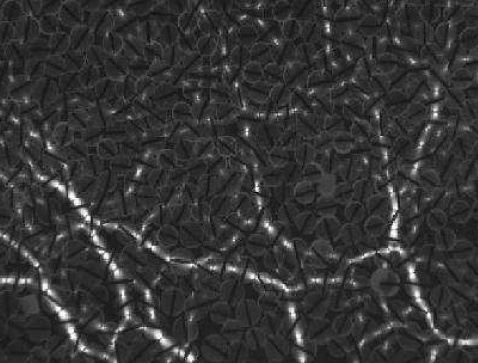
\includegraphics[max width=0.65\linewidth]{../images/utter_force_chains.jpg}\]

\begin{enumerate}
\def\labelenumi{\arabic{enumi})}
\tightlist
\item
  Brian Utter and R. P. Behringer, ``Self-diffusion in dense granular
  shear flows'', \emph{Physical Review E} \textbf{69}, 031308 (2004).
  Also available as
  \href{http://arXiv.org/abs/cond-mat/0402669}{\texttt{arXiv:cond-mat/0402669}}.
\end{enumerate}

I wonder if conformal field theory could help us understand these
simplified \(2\)-dimensional models of granular flow, at least near some
critical point between ``stuck'' and ``unstuck'' flow. Conformal field
theory tends to be good at studying critical points in 2d physics.

Anyway, I'm digressing. After looking at a chaotic double pendulum in
another lab, I talked to Harold Butner about his work using radio
astronomy to study interstellar dust.

He told me that the dust in the Red Rectangle contains a lot of PAHs ---
``polycyclic aromatic hydrocarbons''. These are compounds made of
hexagonal rings of carbon atoms, with some hydrogens along the edges.
\[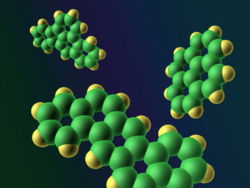
\includegraphics[max width=0.65\linewidth]{../images/PAH_molecules.jpg}\]
On Earth you can find PAHs in soot, or the tarry stuff that forms in a
barbecue grill. Wherever carbon-containing materials suffer incomplete
combustion, you'll find PAHs.

Benzene has a single hexagonal ring, with 6 carbons and 6 hydrogens.
You've probably heard about naphthalene, which is used for mothballs.
This consists of two hexagonal rings stuck together. True PAHs have
more. Anthracene and phenanthrene consist of three rings: \[
  \begin{array}{cc}
    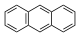
\includegraphics{../images/80px-Anthracene_acsv.svg.png}
    & 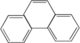
\includegraphics{../images/80px-Phenanthrenec1.png}
  \\\mbox{\href{http://en.wikipedia.org/wiki/Anthracene}{Anthracene}}
    & \mbox{\href{http://en.wikipedia.org/wiki/Phenanthrene}{Phenanthrene}}
  \end{array}
\] Napthacene, pyrene, triphenylene and chrysene consist of four: \[
  \begin{array}{cccc}
    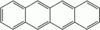
\includegraphics[width=0.2\linewidth]{../images/100px-Tetracene.png}
    & 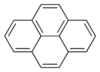
\includegraphics[width=0.2\linewidth]{../images/100px-Pyrene.png}
    & 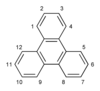
\includegraphics[width=0.2\linewidth]{../images/100px-Triphenylene_chemical_structure.png}
    & 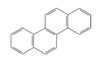
\includegraphics[width=0.2\linewidth]{../images/100px-Chrysene.png}
  \\\mbox{\href{http://en.wikipedia.org/wiki/Tetracene}{Napthacen} (aka Tetracene)}
    & \mbox{\href{http://en.wikipedia.org/wiki/Pyrene}{Pyrene}}
    & \mbox{\href{http://en.wikipedia.org/wiki/Triphenylene}{Triphenylene}}
    & \mbox{\href{http://en.wikipedia.org/wiki/Chrysene}{Chrysene}}
  \end{array}
\] and so on:

\begin{enumerate}
\def\labelenumi{\arabic{enumi})}
\setcounter{enumi}{1}
\tightlist
\item
  Wikipedia, ``Polycyclic aromatic hydrocarbon'',
  \texttt{http://en.wikipedia.org/wiki/Polycyclic\_aromatic\_hydrocarbon}
\end{enumerate}

In 2004, a team of scientists discovered anthracene and pyrene in the
Red Rectangle! This was first time such complex molecules had been found
in space:

\begin{enumerate}
\def\labelenumi{\arabic{enumi})}
\setcounter{enumi}{2}
\tightlist
\item
  Uma P. Vijh, Adolf N. Witt, and Karl D. Gordon, ``Small polycyclic
  aromatic hydrocarbons in the Red Rectangle'', \emph{The Astrophysical
  Journal} \textbf{619} (2005) 368--378. Also available as
  \href{http://arXiv.org/abs/astro-ph/0410130}{\texttt{astro-ph/0410130}}.
\end{enumerate}

By now, lots of organic molecules have been found in interstellar or
circumstellar space. There's a whole ``ecology'' of organic chemicals
out there, engaged in complex reactions. Life on planets might someday
be seen as just an aspect of this larger ecology.

I've read that about 10\% of the interstellar carbon is in the form of
PAHs --- big ones, with about 50 carbons per molecule. They're common
because they're incredibly stable. They've even been found riding the
shock wave of a supernova explosion!

PAHs are also found in meteorites called ``carbonaceous chondrites''.
These space rocks contain just a little carbon --- about 3\% by weight.
But, 80\% of this carbon is in the form of PAHs.

Here's an interview with a scientist who thinks PAHs were important
precursors of life on Earth:

\begin{enumerate}
\def\labelenumi{\arabic{enumi})}
\setcounter{enumi}{4}
\tightlist
\item
  ``Aromatic world'', interview with Pascale Ehrenfreund,
  \emph{Astrobiology Magazine}, available at
  \texttt{http://www.astrobio.net/news/modules.php?op=modload\&name=News\&file=article\&sid=1992}
\end{enumerate}

And here's a book she wrote, with a chapter on organic molecules in
space:

\begin{enumerate}
\def\labelenumi{\arabic{enumi})}
\setcounter{enumi}{5}
\tightlist
\item
  Pascale Ehrenfreud, editor, Astrobiology: Future Perspectives,
  Springer Verlag, 2004.
\end{enumerate}

Harold Butner also told me about dust disks that have been seen around
the nearby stars Vega and Epsilon Eridani. By examining these disks, we
may learn about planets and comets orbiting these stars. Comets emit a
lot of dust, and planets affect its motion.

Mathematicians will be happy to know that \emph{symplectic geometry} is
required to simulate the motion of this dust:

\begin{enumerate}
\def\labelenumi{\arabic{enumi})}
\setcounter{enumi}{6}
\tightlist
\item
  A. T. Deller and S. T. Maddison, ``Numerical modelling of dusty debris
  disks'', \emph{Astrophys. J.} \textbf{625} (2005), 398--413. Also
  available as
  \href{https://arxiv.org/abs/astro-ph/0502135}{\texttt{astro-ph/0502135}}
\end{enumerate}

Okay\ldots{} now for a bit about Hochschild cohomology. I want to
outline a conceptual proof of Deligne's conjecture that the cochain
complex for Hochschild cohomology is an algebra for the little
\(2\)-cubes operad. There are a bunch of proofs of this by now. Here's a
great introduction to the story:

\begin{enumerate}
\def\labelenumi{\arabic{enumi})}
\setcounter{enumi}{7}
\tightlist
\item
  Maxim Kontsevich, ``Operads and motives in deformation quantization'',
  available as
  \href{http://arXiv.org/abs/math/9904055}{\texttt{arXiv:math/9904055}}.
\end{enumerate}

I was inspired to seek a more conceptual proof by some conversations I
had with Simon Willerton in Sheffield this summer, and this paper of
his:

\begin{enumerate}
\def\labelenumi{\arabic{enumi})}
\setcounter{enumi}{8}
\tightlist
\item
  Andrei Caldararu and Simon Willerton, ``The Mukai pairing, I: a
  categorical approach'', available as
  \href{http://arXiv.org/abs/0707.2052}{\texttt{arXiv:0707.2052}}.
\end{enumerate}

But, while trying to write up a sketch of this more conceptual proof, I
discovered that it had already been worked out:

\begin{enumerate}
\def\labelenumi{\arabic{enumi})}
\setcounter{enumi}{9}
\tightlist
\item
  Po Hu, Igor Kriz and Alexander A. Voronov, ``On Kontsevich's
  Hochschild cohomology conjecture'', available at
  \href{http://arXiv.org/abs/math.AT/0309369}{\texttt{arXiv:math.AT/0309369}}.
\end{enumerate}

This was a bit of a disappointment --- but also a relief. It means I
don't need to worry about the technical details: you can just look them
up! Instead, I can focus on sketching the picture I had in mind.

If you don't know anything about Hochschild cohomology, don't worry! It
only comes in at the very end. In fact, the conjecture follows from
something simpler and more general. So, what you really need is a high
tolerance for category theory, homological algebra and operads.

First, suppose we have any monoidal category. Such a category has a
tensor product and a unit object, which we'll call \(I\). Let
\(\mathrm{end}(I)\) be the set of all endomorphisms of this unit object.

Given two such endomorphisms, say \[f\colon I \to I\] and
\[g\colon I \to I\] we can compose them, getting
\[f \circ g\colon I \to I\] This makes \(\mathrm{end}(I)\) into a
monoid. But we can also tensor \(f\) and \(g\), and since
\(I \otimes I\) is isomorphic to \(I\) in a specified way, we can write
the result simply as \[f \otimes g\colon I \to I\] This makes
\(\mathrm{end}(I)\) into a monoid in another, seemingly different way.

Luckily, there's a thing called the Eckmann-Hilton argument which says
these two ways are equal. It also says that \(\mathrm{end}(I)\) is a
\emph{commutative} monoid! It's easiest to understand this argument if
we write \(f \circ g\) vertically, like this: \[
  \begin{array}{c}
    f\\g
  \end{array}
\] and \(f \otimes g\) horizontally, like this: \[
  \begin{array}{cc}
    f&g
  \end{array}
\] Then the Eckmann-Hilton argument goes as follows: \[
  \begin{array}{c}
    f\\g
  \end{array}
  =
  \begin{array}{cc}
    1&f\\g&1
  \end{array}
  =
  \begin{array}{cc}
    g&f
  \end{array}
  =
  \begin{array}{cc}
    g&1\\1&f
  \end{array}
  =
  \begin{array}{c}
    g\\f
  \end{array}
\] Here \(1\) means the identity morphism \(1\colon I \to I\). Each step
in the argument follows from standard stuff about monoidal categories.
In particular, an expression like \[
  \begin{array}{cc}
    f&g\\h&k
  \end{array}
\] is well-defined, thanks to the interchange law
\[(f \otimes g) \circ (h \otimes k) = (f \circ h) \otimes (g \circ k)\]
If we want to show off, we can say the interchange law says we've got a
``monoid in the category of monoids'' --- and the Eckmann-Hilton
argument shows this is just a monoid. See
\protect\hyperlink{week100}{``Week 100''} for more.

But the cool part about the Eckmann-Hilton argument is that we're just
moving \(f\) and \(g\) around each other. So, this argument has a
topological flavor! Indeed, it was first presented as an argument for
why the second homotopy group is commutative. It's all about sliding
around little rectangles\ldots{} or as we'll soon call them, ``little
\(2\)-cubes''.

Next, let's consider a version of this argument that holds only ``up to
homotopy''. This will apply when we have not a \emph{set} of morphisms
from any object \(X\) to any object \(Y\), but a \emph{chain complex} of
morphisms.

Instead of getting a set \(\mathrm{end}(I)\) that's a commutative
monoid, we'll get a cochain complex \(\mathrm{END}(I)\) that's a
commutative monoid ``up to coherent homotopy''. This means that the
associative and commutative laws hold up to homotopies, which satisfy
their own laws up to homotopy, ad infinitum.

More precisely, \(\mathrm{END}(I)\) will be an ``algebra of the little
\(2\)-cubes operad''. This implies that for every configuration of \(n\)
little rectangles in a square: \[
  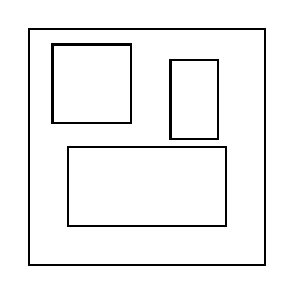
\begin{tikzpicture}
    \draw[thick] (0,0) rectangle ++(3,3);
    \draw[thick] (0.5,0.5) rectangle ++(2,1);
    \draw[thick] (0.3,1.8) rectangle ++(1,1);
    \draw[thick] (1.8,1.6) rectangle ++(0.6,1);
  \end{tikzpicture}
\] we get an \(n\)-ary operation on \(\mathrm{END}(I)\). For every
homotopy between such configurations: \[
  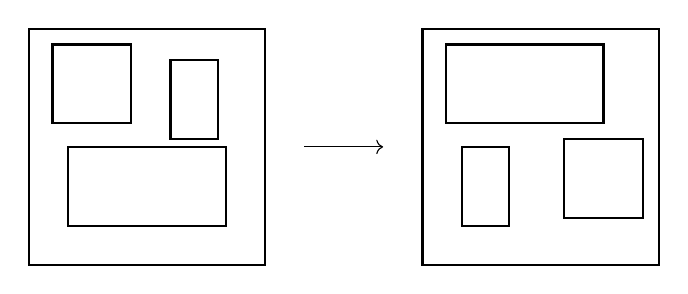
\begin{tikzpicture}
    \draw[thick] (0,0) rectangle ++(3,3);
    \draw[thick] (0.5,0.5) rectangle ++(2,1);
    \draw[thick] (0.3,1.8) rectangle ++(1,1);
    \draw[thick] (1.8,1.6) rectangle ++(0.6,1);
    \draw[->] (3.5,1.5) to (4.5,1.5);
    \begin{scope}[shift={(5,0)}]
    \draw[thick] (0,0) rectangle ++(3,3);
    \draw[thick] (0.3,1.8) rectangle ++(2,1);
    \draw[thick] (1.8,0.6) rectangle ++(1,1);
    \draw[thick] (0.5,0.5) rectangle ++(0.6,1);
    \end{scope}
  \end{tikzpicture}
\] we get a chain homotopy between \(n\)-ary operations on
\(\mathrm{END}(I)\). And so on, ad infinitum.

For more on the little \(2\)-cubes operad, see
\protect\hyperlink{week220}{``Week 220''}. In fact, what I'm trying to
do now is understand some mysteries I described in that article: weird
relationships between the little \(2\)-cubes operad and Poisson
algebras.

But never mind that stuff now. For now, let's see how easy it is to find
situations where there's a cochain complex of morphisms between objects.
It happens throughout homological algebra!

If that sounds scary, you should refer to a book like this as you read
on:

\begin{enumerate}
\def\labelenumi{\arabic{enumi})}
\setcounter{enumi}{9}
\tightlist
\item
  Charles Weibel, \emph{An Introduction to Homological Algebra},
  Cambridge U. Press, Cambridge, 1994.
\end{enumerate}

Okay. First, suppose we have an abelian category. This provides a
context in which we can reason about chain complexes and cochain
complexes of objects. A great example is the category of \(R\)-modules
for some ring \(R\).

Next, suppose every object \(X\) in our abelian category has an
``projective resolution'' --- that is, a chain complex
\[X^0 \xleftarrow{d^0} X^1 \xleftarrow{d^1} X^2 \xleftarrow{d^2} \ldots\]
where each object \(X^i\) is
\href{http://en.wikipedia.org/wiki/Projective_module}{projective}, and
the homology groups
\[H^i = \frac{\ker(d^i)}{\operatorname{im}(d^{i-1})}\] are zero except
for \(H^0\), which equals \(X\). You should think of a projective
resolution as a ``puffed-up'' version of \(X\) that's better for mapping
out of than \(X\) itself.

Given this, besides the usual set \(\operatorname{Hom}(X,Y)\) of
morphisms from the object \(X\) to the object \(Y\), we also get a
cochain complex which I'll call the ``puffed-up hom'':
\[\mathrm{HOM}(X,Y)\] How does this work? Simple: replace \(X\) by a
chosen projective resolution
\[X^0 \leftarrow X^1 \leftarrow X^2 \leftarrow \ldots\] and then map
this whole thing to \(Y\), getting a cochain complex
\[\operatorname{Hom}(X^0,Y) \to \operatorname{Hom}(X^1,Y) \to \operatorname{Hom}(X^2,Y) \to \ldots\]
This cochain complex is the puffed-up hom, \(\mathrm{HOM}(X,Y)\).

Now, you might hope that the puffed-up hom gives us a new category where
the hom-sets are actually cochain complexes. This is morally true, but
the composition
\[\circ\colon \mathrm{HOM}(X,Y) \times \mathrm{HOM}(Y,Z) \to \mathrm{HOM}(X,Z)\]
probably isn't associative ``on the nose''. However, I think it should
be associative up to homotopy! This homotopy probably won't satisfy the
law you'd hope for --- the pentagon identity. But, it should satisfy the
pentagon identity up to homotopy! In fact, this should go on forever,
which is what we mean by ``up to coherent homotopy''. This kind of
situation is described by an infinite sequence of shapes called
``associahedra'', discovered by Stasheff (see
\protect\hyperlink{week144}{``Week 144''}).

If this is the case, instead of a category we get an
``\(A_\infty\)-category'': a gadget where the hom-sets are cochain
complexes and the associative law holds up to coherent homotopy. I'm not
sure the puffed-up hom gives an \(A_\infty\)-category, but let's assume
so and march on.

Suppose we take any object \(X\) in our abelian category. Then we get a
cochain complex \[\mathrm{END}(X) = \mathrm{HOM}(X,X)\] equipped with a
product that's associative up to coherent homotopy. Such a thing is
known as an ``\(A_\infty\)-algebra''. It's just an \(A_\infty\)-category
with a single object, namely \(X\).

Next suppose our abelian category is monoidal. (To get the tensor
product to play nice with the hom, assume tensoring with any object is
\href{http://en.wikipedia.org/wiki/Exact_functor}{right exact}.) Let's
see what happens to the Eckmann-Hilton argument. We should get a version
that holds ``up to coherent homotopy''.

Let I be the unit object, as before. In addition to composition:
\[\circ\colon \mathrm{END}(I) \times \mathrm{END}(I) \to \mathrm{END}(I)\]
tensoring should give us another product:
\[\otimes\colon \mathrm{END}(I) \times \mathrm{END}(I) \to \mathrm{END}(I)\]
which is also associative up to coherent homotopy. So,
\(\mathrm{END}(I)\) should be an \(A_\infty\)-algebra in two ways. But,
since composition and tensoring in our original category get along
nicely:
\[(f \otimes g) \circ (h \otimes k) = (f \circ h) \otimes (g \circ k)\]
\(\mathrm{END}(I)\) should really be an \(A_\infty\)-algebra in the
category of \(A_\infty\)-algebras!

Given this, we're almost done. A monoid in the category of monoids is a
commutative monoid --- that's another way of stating what the
Eckmann-Hilton argument proves. Similarly, an \(A_\infty\)-algebra in
the category of \(A_\infty\)-algebras is an algebra of the little
\(2\)-cubes operad. So, \(\mathrm{END}(I)\) is an algebra of the little
\(2\)-cubes operad.

Now look at an example. Fix some algebra \(A\), and take our monoidal
abelian category to have:

\begin{itemize}
\tightlist
\item
  \((A,A)\)-bimodules as objects
\item
  \((A,A)\)-bimodule homomorphisms as morphisms
\end{itemize}

Here the tensor product is the usual tensor product of bimodules, and
the unit object \(I\) is \(A\) itself. And, as Simon Willerton pointed
out to me, \(\mathrm{END}(I)\) is a cochain complex whose cohomology is
familiar: it's the ``Hochschild cohomology'' of \(A\).

So, the cochain complex for Hochschild cohomology is an algebra of the
little \(2\)-cubes operad! But, we've seen this as a consequence of a
much more general fact.

To wrap up, here are a few of the many technical details I glossed over
above.

First, I said an projective resolution of \(X\) is a puffed-up version
of \(X\) that's better for mapping out of. This idea is made precise in
the theory of model categories. But, instead of calling it a ``puffed-up
version'' of \(X\), they call it a ``cofibrant replacement'' for \(X\).
Similarly, a puffed-up version of \(X\) that's better for mapping into
is called a ``fibrant replacement''.

For a good introduction to this, try:

\begin{enumerate}
\def\labelenumi{\arabic{enumi})}
\setcounter{enumi}{10}
\tightlist
\item
  Mark Hovey, \emph{Model Categories}, American Mathematical Society,
  Providence, Rhode Island, 1999.
\end{enumerate}

Second, I guessed that for any abelian category where every object has a
projective resolution, we can create an \(A_\infty\)-category using the
puffed-up hom, \(\mathrm{HOM}(X,Y)\). Alas, I'm not really sure this is
true.

Hu, Kriz and Voronov consider a more general situation, but what I'm
calling the ``puffed-up hom'' should be a special case of their
``derived function complex''. However, they don't seem to say what
weakened sort of category you get using this derived function complex
--- maybe an \(A_\infty\)-category, or something equivalent like a
quasicategory or Segal category? They somehow sidestep this issue, but
to me it's interesting in its own right.

At this point I should mention something well-known that's similar to
what I've been talking about. I've been talking about the ``puffed-up
hom'' for an abelian category with enough projectives. But most people
talk about ``\(\mathrm{Ext}\)'', which is the cohomology of the
puffed-up hom: \[\mathrm{Ext}^i(X,Y) = H^i(\mathrm{HOM}(X,Y))\] And,
while I want \[\mathrm{END}(X) = \mathrm{HOM}(X,X)\] to be an
\(A_\infty\)-algebra, most people seem happy to have
\[\mathrm{Ext}(X) = H(\mathrm{HOM}(X,X))\] be an \(A_\infty\)-algebra.
Here's a reference:

\begin{enumerate}
\def\labelenumi{\arabic{enumi})}
\setcounter{enumi}{11}
\tightlist
\item
  D.-M. Lu, J. H. Palmieri, Q.-S. Wu and J. J. Zhang,
  ``\(A_\infty\)-structure on \(\mathrm{Ext}\)-algebras'', available as
  \href{http://arXiv.org/abs/math.KT/0606144}{\texttt{arXiv:math.KT/0606144}}.
\end{enumerate}

I hope they're secretly getting this \(A_\infty\)-structure on
\(H(\mathrm{HOM}(X,X))\) from an \(A_\infty\)-structure on
\(\mathrm{HOM}(X,X)\). They don't come out and say this is what they're
doing, but one promising sign is that they use a theorem of Kadeishvili,
which says that the cohomology of an \(A_\infty\)-algebra is an
\(A_\infty\)-algebra.

Finally, the really interesting part: how do we make an
\(A_\infty\)-algebra in the category of \(A_\infty\)-algebras into an
algebra of the little \(2\)-cubes operad? This is the heart of the
``homotopy Eckmann-Hilton argument''.

I explained operads, and especially the little \(k\)-cubes operad, back
in \protect\hyperlink{week220}{``Week 220''}. The little \(k\)-cubes
operad is an operad in the world of topological spaces. It has one
abstract \(n\)-ary operation for each way of sticking \(n\) little
\(k\)-dimensional cubes in a big one, like this: \[
  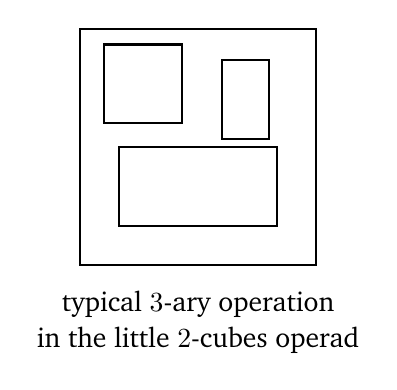
\begin{tikzpicture}
    \draw[thick] (0,0) rectangle ++(3,3);
    \draw[thick] (0.5,0.5) rectangle ++(2,1);
    \draw[thick] (0.3,1.8) rectangle ++(1,1);
    \draw[thick] (1.8,1.6) rectangle ++(0.6,1);
    \node at (1.5,-0.5) {typical $3$-ary operation};
    \node at (1.5,-0.95) {in the little $2$-cubes operad};
  \end{tikzpicture}
\] A space is called an ``algebra'' of this operad if these abstract
\(n\)-ary operations are realized as actual \(n\)-ary operations on the
space in a consistent way. But, when we study the homology of
topological spaces, we learn that any space gives a chain complex. This
lets us convert any operad in the world of topological spaces into an
operad in the world of chain complexes. Using this, it also makes sense
to speak of a \emph{chain complex} being an algebra of the little
\(k\)-cubes operad. Or, for that matter, a cochain complex.

Let's use ``\(E(k)\)'' to mean the chain complex version of the little
\(k\)-cubes operad.

An ``\(A_\infty\)-algebra'' is an algebra of a certain operad called
\(A\)-infinity. This isn't quite the same as the operad \(E(1)\), but
it's so close that we can safely ignore the difference here: it's
``weakly equivalent''.

Say we have an \(A_\infty\)-algebra in the category of
\(A_\infty\)-algebras. How do we get an algebra of the little
\(2\)-cubes operad, \(E(2)\)?

Well, there's a way to tensor operads, such that an algebra of
\(P\otimes Q\) is the same as a \(P\)-algebra in the category of
\(Q\)-algebras. So, an \(A_\infty\)-algebra in the category of
\(A_\infty\)-algebras is the same as an algebra of
\[A_\infty \otimes A_\infty\] Since \(A_\infty\) and \(E(1)\) are weakly
equivalent, we can turn this algebra into an algebra of
\[E(1) \otimes E(1)\] But there's also an obvious operad map
\[E(1) \otimes E(1) \to E(2)\] since the product of two little
\(1\)-cubes is a little \(2\)-cube. This too is a weak equivalence, so
we can turn our algebra of \(E(1) \otimes E(1)\) into an algebra of
\(E(2)\).

The hard part in all this is showing that the operad map
\[E(1) \otimes E(1) \to E(2)\] is a weak equivalence. In fact, quite
generally, the map \[E(k) \otimes E(k') \to E(k+k')\] is a weak
equivalence. This is Proposition 2 in the paper by Hu, Kriz and Voronov,
based on an argument by Gerald Dunn:

\begin{enumerate}
\def\labelenumi{\arabic{enumi})}
\setcounter{enumi}{12}
\tightlist
\item
  Gerald Dunn, ``Tensor products of operads and iterated loop spaces'',
  \emph{Jour. Pure Appl. Alg} \textbf{50} (1988), 237--258.
\end{enumerate}

Using this, they do much more than what I've sketched: they prove a
conjecture of Kontsevich which says that the Hochschild complex of an
algebra of the little \(k\)-cubes operad is an algebra of the little
\((k+1)\)-cubes operad!

That's all for now. Sometime I should tell you how this is related to
Poisson algebras, 2d TQFTs, and much more. But for now, you'll have to
read that in Kontsevich's very nice paper.

\begin{center}\rule{0.5\linewidth}{0.5pt}\end{center}

\textbf{Addenda:} Over at the \(n\)-Category Café, Michael Batanin made
some comments on the difficulties in making my proposed argument
rigorous, his own work in doing just this (long before I came along),
and the history of Deligne's conjecture (which I deliberately didn't go
into, since it's such a long story). Mikael Vejdemo Johansson explained
more about the \(A_\infty\)-structure on Ext.

Modulo some typographical changes, Michael Batanin wrote:

\begin{quote}
Hi, John.

Just a few remarks about your stuff on Deligne's conjecture.
Unfortunately, technical details are important in this business.

First, we have to be careful about tensor product of operads. A very
long standing question is: Let \(A\) be a \(E_1\)-operad and \(B\) be a
cofibrant \(E_1\)-operad. Is it true that their tensor product
\(A \otimes B\) is an \(E_2\)-operad? The answer is unknown, even though
Dunn's argument is correct and the tensor product of two little
\(1\)-cube operads is equivalent to the little \(2\)-cube operad.
Unfortunately, the theorem from Hu, Kriz and Voronov is based implicitly
on an affirmative answer to the above question.

I think the history of Deligne's conjecture is quite remarkable and
complicated and still developing. The most conceptual and correct proof
I know is provided by Tamarkin in

\begin{enumerate}
\def\labelenumi{\arabic{enumi})}
\setcounter{enumi}{13}
\tightlist
\item
  Dmitry Tamarkin, ``What do DG categories form?'', available as
  \href{http://arXiv.org/abs/math.CT/0606553}{\texttt{math.CT/0606553}}.
\end{enumerate}

And it uses my up to homotopy Eckmann--Hilton argument. This argument is
based on a techniques of compactification of configuration spaces and
first was proposed by Getzler and Jones. I think I already wrote about
it in a post to \(n\)-category cafe where Dolgushev's work was
discussed. Here is the reference to my lecture about Deligne's
conjecture:

\begin{enumerate}
\def\labelenumi{\arabic{enumi})}
\setcounter{enumi}{14}
\tightlist
\item
  Michael A. Batanin, ``Deligne's conjecture: an interplay between
  algebra, geometry and higher category theory'', talk at ANU Canberra,
  November 3 2006, available at
  \texttt{http://www.math.mq.edu.au/\textasciitilde{}street/BataninMPW.pdf}
\end{enumerate}

Concerning your idea to construct an \(A\)-infinity category using
\(\mathrm{Hom}(PX,Y)\), where \(PX\) is a projective resolution: it's
been done by me many years ago and in a more general situation. It is
long story to tell but more or less I prove that your Hom functor is
equivalent as a simplicially coherent bimodule to the homotopy coherent
left Kan extension of the inclusion functor
\[\text{Projective bounded chain complex} \to \text{Bounded chain complex}\]
along itself. Then the Kleisli category of this distributor has a
canonical \(A\)-infinity structure and this Kleisli category is
equivalent in an appropriate sense to your `puffed' category. In fact,
the situation I consider in my paper is much more general and includes
simplicial Quillen categories as a very special example. The paper is:

\begin{enumerate}
\def\labelenumi{\arabic{enumi})}
\setcounter{enumi}{15}
\tightlist
\item
  Michael A. Batanin, ``Categorical strong shape theory'', \emph{Cahiers
  de Topologie et Geom. Diff.} \textbf{V.XXXVIII-1} (1997), 3--67.
\end{enumerate}

and its companion

\begin{enumerate}
\def\labelenumi{\arabic{enumi})}
\setcounter{enumi}{16}
\tightlist
\item
  Michael A. Batanin, ``Homotopy coherent category theory and
  \(A_\infty\) structures in monoidal categories'', \emph{Jour. Pure
  Appl. Alg.} \textbf{123} (1998), 67--103.
\end{enumerate}

Regards,\\
Michael
\end{quote}

Batanin's talk has a very nice introduction to his ``derived
Eckmann-Hilton argument'', which is a precise version of what I was
attempting to sketch in this Week's Finds. Here's the paper by Getzler
and Jones:

\begin{enumerate}
\def\labelenumi{\arabic{enumi})}
\setcounter{enumi}{17}
\tightlist
\item
  Ezra Getzler and J. D. S. Jones, ``Operads, homotopy algebra and
  iterated integrals for double loop spaces'', available as
  \href{http://arXiv.org/abs/hep-th/9403055}{\texttt{hep-th/9403055}}.
\end{enumerate}

It's very interesting, but it was never published, perhaps because of
some subtle flaws caught by Tamarkin.

Modulo some typographical changes and extra references, Mikael Vejdemo
Johansson wrote:

\begin{quote}
I could try to claim that I'm starting to become an expert on things
\(A_\infty\), but given that Jim Stasheff is an avid commenter here, I
don't quite dare to. :)

However, I have read the Lu-Palmieri-Wu-Zhang {[}LPWZh{]} paper
mentioned in the exposition backwards and forwards. On the face, what
LPWZh try to do is to take the survey articles by Bernhard Keller:

\begin{enumerate}
\def\labelenumi{\arabic{enumi})}
\setcounter{enumi}{18}
\item
  Bernhard Keller, Introduction to \(A_\infty\)-algebras and modules,
  available as
  \href{http://arxiv.org/abs/math/9910179}{\texttt{arXiv:math/9910179}}.

  ``A brief introduction to \(A_\infty\)-algebras'', notes from a talk
  at the workshop on \emph{Derived Categories, Quivers and Strings},
  Edinburgh, August 2004. Available at
  \texttt{http://www.institut.math.jussieu.fr/\textasciitilde{}keller/publ/index.html}

  ``\(A_\infty\)-algebras in representation theory'', contribution to
  the \emph{Proceedings of ICRA IX, Beijing 2000}. Available at
  \texttt{http://www.institut.math.jussieu.fr/\textasciitilde{}keller/publ/index.html}

  ``\(A_\infty\)-algebras, modules and functors'', available as
  \href{http://arxiv.org/abs/math/0510508}{\texttt{arXiv:math/0510508}}.
\end{enumerate}

outlining the use of \(A_\infty\)-algebras in representation theory, and
widening the scope of their proven usability while actually proving the
many unproven and interesting statements that Keller makes.

At the core of this lies two different theorems. One is the Kadeishvili
theorem (which in various guises has been proven by everyone involved
with \(A_\infty\)-algebras, and a few more, in my impression ;) that
says that you can carry \(A_\infty\)-algebras across taking homology.
Kadeishvili's argument specializes to the case where you start with an
\(A_\infty\)-algebra with only \(m_1\) and \(m_2\) are non-trivial ---
i.e.~a plain old dg-algebra. For higher generality, you'd probably want
to turn to the Homology Perturbation Theory crowd with Stasheff,
Gugenheim and Huebschmann among the more famous names\ldots{}

Hence, if we take graded endomorphism algebra of a resolution of \(M\)
and introduce the ``homotopy differential'': \[\partial f = d f + f d\]
then cycles are chain maps and the homology picks out exactly the
algebra cohomology over the appropriate module category. Thus, we get
\(\mathrm{Ext}\) as the homology of a dg-algebra, and thus,
\(\mathrm{Ext}\) has an \(A_\infty\)-algebra structure.

The second cornerstone of these papers is the Keller higher
multiplication theorem: if the ring \(R\) is sufficiently nice, then the
\(A_\infty\)-algebra structure on \(\mathrm{Ext}_R^*(M,M)\) for some
appropriate module \(M\) will allow you to recover a presentation of
\(R\) explicitly.

I hope this answers your question about the origin of their
\(A_\infty\)-algebra structure.
\end{quote}

Note the great technical simplification of working with what I called
\(\operatorname{Hom}(PX,PX)\) instead of \(\operatorname{Hom}(PX,X)\)
--- composition becomes strictly associative!

For more discussion, go to the
\href{http://golem.ph.utexas.edu/category/2007/11/this_weeks_finds_in_mathematic_22.html}{\(n\)-Category
Café}.

\begin{center}\rule{0.5\linewidth}{0.5pt}\end{center}

\begin{quote}
\emph{We need a really short and convincing argument for this very
fundamental fact about the Hochschild complex.}

--- Maxim Kontsevich
\end{quote}

\begin{quote}
\emph{Higher category theory provides us with the argument Kontsevich
was looking for.}

--- Michael Batanin
\end{quote}



\hypertarget{week259}{%
\section{December 9, 2007}\label{week259}}

This week I'll talk about the ``field with one element'' --- even though
it doesn't exist. It's a mathematical phantom.

But first: the Egg Nebula.

In \protect\hyperlink{week257}{``Week 257''} and
\protect\hyperlink{week258}{``Week 258''} I talked about interstellar
dust. As I mentioned, lots of it comes from ``asymptotic giant branch''
stars --- stars like our Sun, but later in their life, when they're big,
red, pulsing, and puffing out elements like hydrogen, helium, carbon,
nitrogen, and oxygen.

The pulsations grow wilder and wilder until the star blows off its
entire outer atmosphere, forming a big cloud of gas and dust
misleadingly called a ``planetary nebula''. It leaves behind its dense
inner core as a hot white dwarf. Intense radiation from this core
eventually heats the gas and dust until they glow.

Back in \protect\hyperlink{week223}{``Week 223''} I showed my favorite
example of a planetary nebula: the Cat's Eye.
\[\href{http://heritage.stsci.edu/2004/27/index.html}{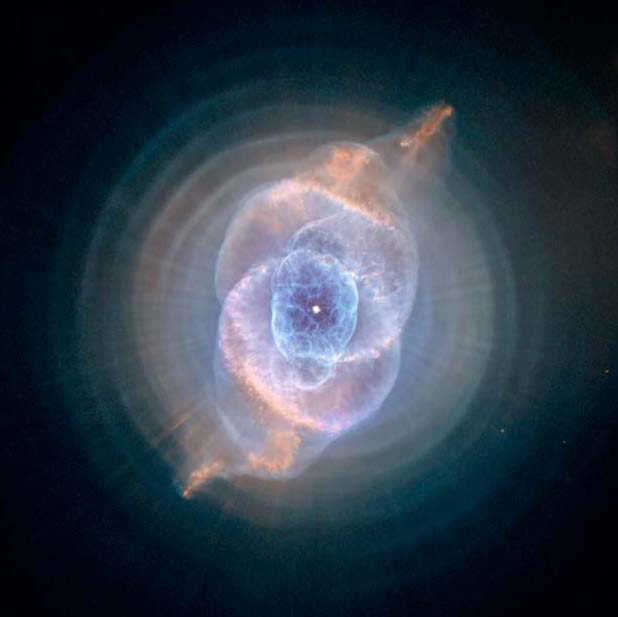
\includegraphics[max width=0.65\linewidth]{../images/cats-eye_nebula.jpg}}\]
And I quoted the astronomer Bruce Balick on what will happen here when
our Sun becomes a planetary nebula 6.9 billion years from now:

\begin{quote}
Here on Earth, we'll feel the wind of the ejected gases sweeping past,
slowly at first (a mere 5 miles per second!), and then picking up speed
as the spasms continue --- eventually to reach 1000 miles per second!!
The remnant Sun will rise as a dot of intense light, no larger than
Venus, more brilliant than 100 present Suns, and an intensely hot
blue-white color hotter than any welder's torch. Light from the fiendish
blue ``pinprick'' will braise the Earth and tear apart its surface
molecules and atoms. A new but very thin ``atmosphere'' of free
electrons will form as the Earth's surface turns to dust.
\end{quote}

Eerie!

Here's a ``protoplanetary nebula'' --- that is, a planetary nebula
that's just getting started:
\[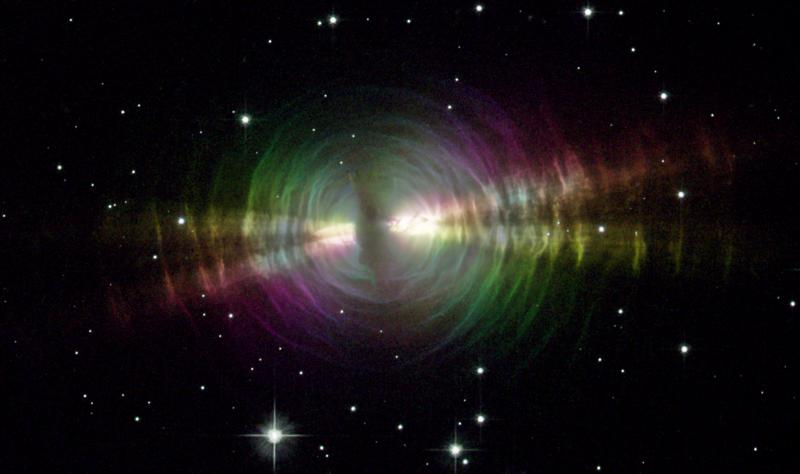
\includegraphics[max width=0.65\linewidth]{../images/egg_nebula.jpg}\]

\begin{enumerate}
\def\labelenumi{\arabic{enumi})}
\tightlist
\item
  ``Rainbow image of a dusty star'', NASA,
  \texttt{http://hubblesite.org/newscenter/archive/releases/nebula/planetary/2003/09/}
\end{enumerate}

It's called the ``Egg Nebula''. You can see layers of dust coming out
puff after puff, shooting outwards at about 20 kilometers per second,
stretching out for about a third of a light year. The colors --- red,
green and blue --- aren't anything you'd actually see. They're just an
easy way to depict three different polarizations of light. I don't know
why the light is polarized that way.

You can see a dark disk of thicker dust running around the star. It
could be an ``accretion disk'' spiralling into the star. The ``beams''
shining out left and right are still poorly understood. Maybe they're
jets of matter ejected from the north and south poles of the disk? This
idea seem more plausible when you look at this photo taken by NICMOS,
which is Hubble's ``Near Infrared Camera and Multi-Object
Spectrometer'':
\[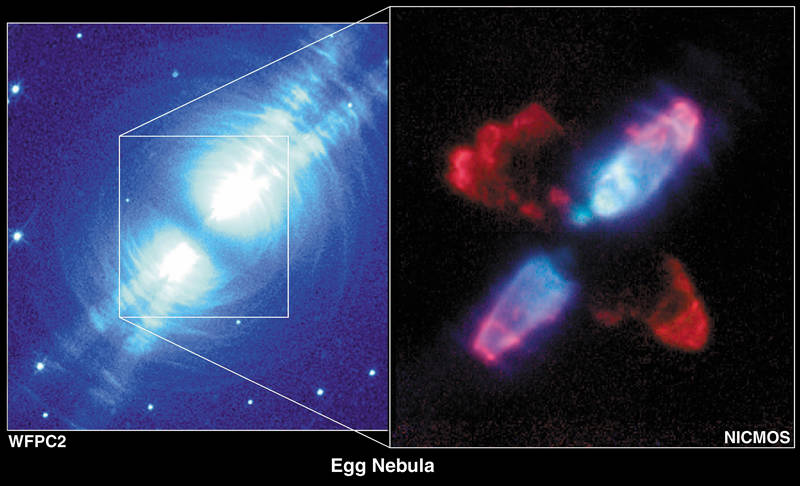
\includegraphics[max width=0.65\linewidth]{../images/egg_nebula_infrared.jpg}\]

\begin{enumerate}
\def\labelenumi{\arabic{enumi})}
\setcounter{enumi}{1}
\tightlist
\item
  Raghvendra Sahai, ``Egg Nebula in polarized light'', Hubble Heritage
  Project, \texttt{http://heritage.stsci.edu/2003/09/supplemental.html}
\end{enumerate}

This near-infrared image also shows a bright spot called ``Peak A''
about 500 AU from the central star. An ``AU'', or astronomical unit, is
the distance from the Sun to the Earth.

Nobody knows what this bright spot is. Some argue that it's just a clump
of dust reflecting light from the main star. Others advocate a more
exciting theory: it's a white dwarf orbiting the main star, which
exploded in a ``thermonuclear burst'' after accreting a bunch of dust.

\begin{enumerate}
\def\labelenumi{\arabic{enumi})}
\setcounter{enumi}{2}
\tightlist
\item
  Joel H. Kastner and Noam Soker, ``The Egg Nebula (AFGL 2688):
  deepening enigma'', to appear in \emph{Asymmetrical Planetary Nebulae
  III}, eds.~M. Meixner, J. Kastner, N. Soker, and B. Balick, ASP
  Conference Series. Available as
  \href{http://arXiv.org/abs/astro-ph/0309677}{\texttt{astro-ph/0309677}}.
\end{enumerate}

I hope to say more about planetary nebulae in future Weeks, mainly
because they're so beautiful.

But now: the field with one element!

A \href{http://en.wikipedia.org/wiki/Field_\%28mathematics\%29}{field}
is a mathematical structure where you can add, multiply, subtract and
divide in ways that satisfy these familiar rules:

\begin{itemize}
\tightlist
\item
  \(x + y = y + x\)
\item
  \((x + y) + z = x + (y + z)\)
\item
  \(x + 0 = x\)
\item
  \(xy = yx\)
\item
  \((xy)z = x(yz)\)
\item
  \(1x = x\)
\item
  \(x(y + z) = xy + xz\)
\item
  every element \(x\) has an element \(-x\) with \(x + (-x) = 0\)
\item
  every element \(x\) that's not \(0\) has an element \(1/x\) with
  \(x (1/x) = 1\)
\end{itemize}

You'll note that the last clause is the odd man out. Addition,
subtraction and multiplication can all be described as everywhere
defined operations. Division cannot, since we can't divide by \(0\).
This is the funny thing about fields, which is what causes the problem
we'll run into.

Everyone who has studied math knows three examples of fields: the
rational numbers \(\mathbb{Q}\), the real numbers \(\mathbb{R}\) and the
complex numbers \(\mathbb{C}\). There are a lot more, too --- for
example, function fields, number fields, and finite fields.

Let me say a tiny bit about these three kinds of fields.

The simplest sort of
``\href{http://en.wikipedia.org/wiki/Function_field_of_an_algebraic_variety}{function
field}'' consists of rational functions of one variable --- that is,
ratios of polynomials, like this: \[\frac{2z^3 + z + 1}{z^2 - 7}\] Here
the coefficients of your polynomials should lie in some field
\(\mathbb{F}\) you already know about. The resulting field is called
\(\mathbb{F}(z)\). If \(\mathbb{F}\) is the complex numbers, we can
think of \(\mathbb{F}(z) = \mathbb{C}(z)\) as consisting of functions on
the Riemann sphere. In \protect\hyperlink{week201}{``Week 201''}, I
explained how the symmetries of this field form a group important in
special relativity: the Lorentz group!

It's also very interesting to study the field of functions on a surface
fancier than the sphere, but still defined by algebraic equations, like
the surface of a doughnut or \(n\)-holed doughnut. Number theorists and
algebraic geometers spend a lot of time thinking about these fields,
which are called ``function fields of complex curves''.

For example, different ways of describing the surface of a doughnut by
algebraic equations give different
``\href{http://en.wikipedia.org/wiki/Elliptic_curve}{elliptic curves}''.
This is terminology is bound to puzzle beginners! They're called
``curves'' even though it's \(2\)-dimensional, because it takes one
\emph{complex} number to say where you are on a little patch of a
surface, just as it takes one \emph{real} number to say where you are on
an ordinary curve like a circle. That's the origin of the term ``complex
curve''. And, they're called ``elliptic'' because they first showed up
when people were studying elliptic integrals, which are generalizations
of trig functions from circles to ellipses.

I explained more about elliptic curves in
\protect\hyperlink{week13}{``Week 13''} and
\protect\hyperlink{week125}{``Week 125''}. Lurking behind this, there's
a lot of fascinating stuff about function fields of elliptic curves.

The simplest sort of
``\href{http://en.wikipedia.org/wiki/Algebraic_number_field}{number
field}'' comes from taking the rational numbers and throwing in the
solutions of a polynomial equation. For example, in
\protect\hyperlink{week20}{``Week 20''} I talked about the ``golden
field'', which consists of all numbers of the form \[a + b\sqrt{5}\]
where \(a\) and \(b\) are rational.

One of the most beautiful ideas in math is the analogy between number
fields and function fields --- the idea that numbers are like functions
on some sort of ``space''. I began explaining this in
\protect\hyperlink{week205}{``Week 205''},
\protect\hyperlink{week216}{``Week 216''} and
\protect\hyperlink{week218}{``Week 218''}, but there's much more to say
about what's known\ldots{} and also many things that remain mysterious.

In particular, it's pretty well understood how number fields resemble
function fields of complex curves, and how this relates number theory to
\emph{\(2\)-dimensional} topology. But, there are also many analogies
between number theory and \emph{\(3\)-dimensional} topology, which I
began listing in \protect\hyperlink{week257}{``Week 257''}. It seems
these analogies are doomed to remain mysterious until we get a handle on
the field with one element. But more on that later.

The simplest sort of
``\href{http://en.wikipedia.org/wiki/Finite_field}{finite field}'' comes
from choosing a prime number \(p\) and taking the integers modulo \(p\).
The result is sometimes called \(\mathbb{Z}/p\), especially when you're
just concerned with addition. But when you think of it as a field, it's
better to call it \(\mathbb{F}_p\).

The reason is that there's a finite field of size \(q\) whenever \(q\)
is a \emph{power} of a prime, and this field is unique --- so it's
called \(\mathbb{F}_q\). You build \(\mathbb{F}_q\) sort of like how you
build the complex numbers starting from the real numbers, or number
fields starting from the rational numbers. Namely, to construct
\(\mathbb{F}_{p^n}\), you take \(\mathbb{F}_p\) and throw in the roots
of a well-chosen polynomial of degree \(n\): one that doesn't have any
roots in \(\mathbb{F}_p\), but ``wants'' to have \(n\) different roots.

Okay: that was a tiny bit about function fields, number fields and
finite fields. But now I need to point out some slight lies I told!

I said there was a finite field with \(q\) elements whenever \(q\) was a
prime power. You might think this should include \(q = 1\), since \(1\)
is the \emph{zeroth} power of \emph{any} prime.

So, is there a field with one element?

If so, it must have \(1 = 0\). That doesn't violate the definition of a
field that I gave you\ldots{} does it? The definition said any element
that's not \(0\) has a reciprocal. In this particular example, \(0\)
also has a reciprocal, since we can set \(1/0 = 1\) and not get into any
contradictions. But that's not a problem: in usual math practice, saying
``we can divide by anything that's not zero'' doesn't deny the
possibility that we can divide by \(0\).

Unfortunately, allowing a field with \(1 = 0\) causes nothing but grief.
For example, we can define vector spaces using any field (people say
``over'' any field), and there's a nice theorem saying two vector spaces
are isomorphic if and only if they have the same dimension. And
normally, there's one vector space of each dimension. But the last part
isn't true for a field with \(1 = 0\). In a vector space over such a
field, every vector \(v\) has \[v = 1 v = 0 v = 0\] So, every vector
space is \(0\)-dimensional!

To prevent such problems, people add one extra clause to the definition
of a field:

\begin{itemize}
\tightlist
\item
  \(1\) is not equal to \(0\)
\end{itemize}

This clause looks even more tacked-on and silly than the clause saying
everything \emph{nonzero} has a reciprocal\ldots{} but it works fairly
well.

However, the field with one element still wants to exist! Not the silly
field with \(1 = 0\), but something else, something more
mysterious\ldots{} something that Gavin Wraith calls a ``mathematical
phantom'':

\begin{enumerate}
\def\labelenumi{\arabic{enumi})}
\setcounter{enumi}{3}
\tightlist
\item
  Gavin Wraith, ``Mathematical phantoms'',
  \texttt{http://www.wra1th.plus.com/gcw/rants/math/MathPhant.html}
\end{enumerate}

What's a mathematical phantom? According to Wraith, it's an object that
doesn't exist within a given mathematical framework, but nonetheless
``obtrudes its effects so convincingly that one is forced to concede a
broader notion of existence''.

Like a genie that talks its way out of a bottle, a sufficiently powerful
mathematical phantom can talk us into letting it exist by promising to
work wonders for us. Great examples include the number zero, irrational
numbers, negative numbers, imaginary numbers, and quaternions. At one
point all these were considered highly dubious entities. Now they're
widely accepted. They ``exist''. Someday the field with one element will
exist too!

Why?

I gave a lot of reasons in \protect\hyperlink{week183}{``Week 183''},
\protect\hyperlink{week184}{``Week 184''},
\protect\hyperlink{week185}{``Week 185''},
\protect\hyperlink{week186}{``Week 186''} and
\protect\hyperlink{week187}{``Week 187''}, but let me rapidly summarize.

It's all about ``\(q\)-deformation''. In physics, people talk about
\(q\)-deformation when they're taking groups and turning them into
``quantum groups''. But it has a closely related aspect that's in some
ways more fundamental. When we count things involving \(n\)-dimensional
vector spaces over the finite field \(\mathbb{F}_q\), we often get
answers that are polynomials in \(q\). If we then set \(q = 1\), the
resulting formulas count analogous things involving \(n\)-element sets!

So, finite sets want to be finite-dimensional vector spaces over the
(nonexistent) field with one element\ldots{} or something like that. We
can be more precise after looking at some examples.

Here's the simplest example. Say we count lines through the origin in an
\(n\)-dimensional vector space over \(\mathbb{F}_q\). We get the
``\(q\)-integer'' \[\frac{q^n-1}{q-1} = 1+q+q^2+\ldots+q^{n-1}\] which
I'll write as \([n]\) for short.

Setting \(q = 1\), we get \(n\). This is the number of points in an
\(n\)-element set. Sure, that sounds silly. But, I'm trying to make a
point here! At \(q = 1\), stuff about \(n\)-dimensional vector spaces
over \(\mathbb{F}_q\) reduces to stuff about \(n\)-element sets, and the
\(q\)-integer \([n]\) reduces to the ordinary integer \(n\).

This may not be the best way to understand the pattern, though. Lines
through the origin in an \(n\)-dimensional vector space are the same as
points in an \((n-1)\)-dimensional projective space. So, the real
analogy may be between ``points in a projective space'' and ``points in
a set''.

Here's a more impressive example. Pick any uncombed Young diagram \(D\)
with \(n\) boxes. Here's one with 8 boxes: \[
  \begin{array}{lll}
    \square
  \\\square&\square
  \\\square&\square&\square
  \\\square&\square
  \end{array}
\] This has

\begin{itemize}
\tightlist
\item
  1 box in the first row,
\item
  3 boxes in the first two rows,
\item
  6 boxes in the first three rows,
\item
  8 boxes in the first four rows.
\end{itemize}

Then, count the ``\(D\)-flags on an \(n\)-dimensional vector space over
\(\mathbb{F}_q\)''. In our example, such a \(D\)-flag is:

\begin{quote}
a \(1\)-dimensional subspace\\
of a \(3\)-dimensional subspace\\
of a \(6\)-dimensional subspace\\
of a \(8\)-dimensional vector space over \(\mathbb{F}_q\)
\end{quote}

If you actually count these \(D\)-flags you'll get some formula, which
is a polynomial in \(q\). And when you set \(q = 1\), you'll get the
number of ``\(D\)-flags on an \(n\)-element set''. In our example, such
a \(D\)-flag is:

\begin{quote}
a \(1\)-element subset\\
of a \(3\)-element subset\\
of a \(6\)-element subset\\
of a \(8\)-element set
\end{quote}

For details, and a proof that this really works, try:

\begin{enumerate}
\def\labelenumi{\arabic{enumi})}
\setcounter{enumi}{4}
\tightlist
\item
  John Baez, ``Lecture 4'' in the \emph{Geometric Representation Theory
  Seminar}, October 9, 2007. Available at
  \texttt{http://math.ucr.edu/home/baez/qg-fall2007/qg-fall2007.html\#f07\_4}
\end{enumerate}

These examples can be generalized. In \protect\hyperlink{week187}{``Week
187''} I showed how to get one example for each subset of the dots in
any Dynkin diagram! This idea goes back to Jacques Tits, who was the
first to suggest that there should be a field with one element. Dynkin
diagrams give algebraic groups over \(\mathbb{F}_q\)\ldots{} but he
noticed that these groups reduce to ``Coxeter groups'' as \(q \to 1\).
And, if you mark some dots on a Dynkin diagram you get a ``flag
variety'' on which your algebraic group acts\ldots{} but as \(q \to 1\),
this reduces to a finite set on which your Coxeter group acts.

If you don't understand the previous paragraph, don't worry --- it's
over now. It's great stuff, but my main point is that there seems to be
an analogy like this:

\begin{longtable}[]{@{}ll@{}}
\toprule
\begin{minipage}[b]{0.22\columnwidth}\raggedright
\(q = 1\)\strut
\end{minipage} & \begin{minipage}[b]{0.72\columnwidth}\raggedright
\(q = p^n\) for \(p\) prime\strut
\end{minipage}\tabularnewline
\midrule
\endhead
\begin{minipage}[t]{0.22\columnwidth}\raggedright
\(n\)-element set\strut
\end{minipage} & \begin{minipage}[t]{0.72\columnwidth}\raggedright
\((n-1)\)-dimensional projective space over \(\mathbb{F}_q\)\strut
\end{minipage}\tabularnewline
\begin{minipage}[t]{0.22\columnwidth}\raggedright
integer \(n\)\strut
\end{minipage} & \begin{minipage}[t]{0.72\columnwidth}\raggedright
\(q\)-integer \([n]\)\strut
\end{minipage}\tabularnewline
\begin{minipage}[t]{0.22\columnwidth}\raggedright
permutation groups \(S_n\)\strut
\end{minipage} & \begin{minipage}[t]{0.72\columnwidth}\raggedright
projective special linear group \(\mathrm{PSL}(n,\mathbb{F}_q)\)\strut
\end{minipage}\tabularnewline
\begin{minipage}[t]{0.22\columnwidth}\raggedright
factorial \(n!\)\strut
\end{minipage} & \begin{minipage}[t]{0.72\columnwidth}\raggedright
\(q\)-factorial \([n]!\)\strut
\end{minipage}\tabularnewline
\bottomrule
\end{longtable}

This opens up lots of questions. For example, if projective spaces over
\(\mathbb{F}_1\) are just finite sets, what should \emph{vector spaces}
over \(\mathbb{F}_1\) be?

People have thought about this, and the answer seems to be ``pointed
sets'' --- sets with a distinguished point, which you can think of as
the ``origin''. A pointed set with \(n+1\) elements seems to act like an
\(n\)-dimensional vector space over \(\mathbb{F}_q\).

For more clues, and an attempt to do algebraic geometry using the field
with one element, try this:

\begin{enumerate}
\def\labelenumi{\arabic{enumi})}
\setcounter{enumi}{5}
\tightlist
\item
  Christophe Soulé, ``On the field with one element'', Talk given at the
  \emph{Arbeitstagung}, Bonn, June 1999, IHES preprint available at
  \texttt{http://www.ihes.fr/\textbackslash{}\textasciitilde{}soule/f1-soule.pdf}
\end{enumerate}

Soulé tries to define ``algebraic varieties'' over \(\mathbb{F}_1\),
namely curves and their higher-dimensional generalization. And, he talks
a lot about zeta functions for such varieties. He goes into more detail
here:

\begin{enumerate}
\def\labelenumi{\arabic{enumi})}
\setcounter{enumi}{6}
\tightlist
\item
  Christophe Soulé, ``Les varietes sur le corps a un element'',
  \emph{Moscow Math. Jour.} \textbf{4} (2004), 217--244, 312.
\end{enumerate}

The theme of zeta functions --- see \protect\hyperlink{week216}{``Week
216''} --- is deeply involved in this business. For more, try these
papers:

\begin{enumerate}
\def\labelenumi{\arabic{enumi})}
\setcounter{enumi}{7}
\item
  N. Kurokawa, \(Zeta functions over \mathbb{F}_1\), \emph{Proc. Japan
  Acad. Ser. A Math. Sci.} \textbf{81} (2006), 180--184.
\item
  Anton Deitmar, ``Remarks on zeta functions and K-theory over
  \(\mathbb{F}_1\)'', available as
  \href{http://arXiv.org/abs/math/0605429}{\texttt{arXiv:math/0605429}}.
\end{enumerate}

But instead of talking about zeta functions, I'd like to talk about two
approaches to giving a formal definition of the field with one element.
Both of them involve taking the concept of field and modifying it so it
doesn't necessary involve the operation of addition. The first one, due
to Deitmar, simply throws out addition! The second, due to Nikolai
Durov, allows for a wide choice of operations --- and thus a wide supply
of ``exotic fields''.

For Deitmar's approach, try these:

\begin{enumerate}
\def\labelenumi{\arabic{enumi})}
\setcounter{enumi}{9}
\item
  Anton Deitmar, ``Schemes over \(\mathbb{F}_1\)'', available as
  \href{http://arXiv.org/abs/math/0404185}{\texttt{arXiv:math/0404185}}.

  \(\mathbb{F}_1\)-schemes and toric varieties, available as
  \href{http://arXiv.org/abs/math/0608179}{\texttt{arXiv:math/0608179}}.
\end{enumerate}

The usual approach to fields treats fields as specially nice commutative
rings. A
``\href{http://en.wikipedia.org/wiki/Commutative_ring}{commutative
ring}'' is a gadget where you can add and multiply, and these rules
hold:

\begin{itemize}
\tightlist
\item
  \(x + y = y + x\)
\item
  \((x + y) + z = x + (y + z)\)
\item
  \(x + 0 = x\)
\item
  \(xy = yx\)
\item
  \((xy)z = x(yz)\)
\item
  \(1x = x\)
\item
  \(x(y + z) = xy + xz\)
\item
  every element \(x\) has an element \(-x\) with \(x + (-x) = 0\)
\end{itemize}

Deitmar throws out addition and treats fields as specially nice
commutative monoids. A commutative
``\href{http://en.wikipedia.org/wiki/Commutative_ring}{monoid}'' is a
gadget where you can multiply, and these rules hold:

\begin{itemize}
\tightlist
\item
  \(xy = yx\)
\item
  \((xy)z = x(yz)\)
\item
  \(1x = x\)
\end{itemize}

For Deitmar, the field with one element, \(\mathbb{F}_1\), is just the
commutative monoid with one element, namely \(1\). A ``vector space over
\(\mathbb{F}_1\)'' is just a set on which this monoid acts via
multiplication\ldots{} but that amounts to just a plain old set. The
``dimension'' of such a ``vector space'' is just its cardinality.

All this so far is quite trivial, but Deitmar makes a nice attempt at
redoing algebraic geometry to include this field with one element. One
reason to do this is to understand the mysterious \(3\)-dimensional
aspect of number theory.

To explain this, I need to say a bit about
``\href{http://en.wikipedia.org/wiki/Scheme_\%28mathematics\%29}{schemes}''.
In ordinary algebraic geometry, we turn commutative rings into spaces to
think about them geometrically. I explained this back in
\protect\hyperlink{week199}{``Week 199''} and
\protect\hyperlink{week205}{``Week 205''}, but let me review quickly,
and go further:

We can think of elements of a commutative ring \(R\) as functions on
certain space called the
``\href{http://en.wikipedia.org/wiki/Spectrum_of_a_ring}{spectrum}'' of
\(R\), \(\operatorname{Spec}(R)\). This space has a topology, so we can
also talk about functions that are defined, not on all of
\(\operatorname{Spec}(R)\), but just \emph{part} of
\(\operatorname{Spec}(R)\) --- namely some open set. Indeed, for each
open set \(U\) in \(\operatorname{Spec}(R)\), there's a commutative ring
\(\mathcal{O}(U)\) consisting of those functions defined on \(U\). These
commutative rings are related in nice ways:

\begin{enumerate}
\def\labelenumi{\arabic{enumi}.}
\tightlist
\item
  If the open set \(V\) is smaller than \(U\), we can restrict functions
  from \(U\) to \(V\), getting a ring homomorphism
  \(\mathcal{O}(U) \to \mathrm{O}(V)\)
\item
  If \(U\) is covered by a bunch of open sets \(U_i\), and we have a
  function \(f_i\) in each \(\mathcal{O}(U_i)\), such that \(f_i\) and
  \(f_j\) agree when restricted to the set \(U_i \cap U_j\), then
  there's a unique function \(f\) in \(\mathcal{O}(U)\) that restricts
  to each of these functions \(f_i\).
\end{enumerate}

Something satisfying condition 1 is called a
``\href{http://en.wikipedia.org/wiki/Presheaf\#Definition_of_a_presheaf}{presheaf}''
of commutative rings; something also satisfying condition 2 is called a
``\href{http://en.wikipedia.org/wiki/Sheaf_\%28mathematics\%29}{sheaf}''
of commutative rings.

So, \(\operatorname{Spec}(R)\) is not just a topological space, it's
equipped with a sheaf of commutative rings. People call this a
``\href{http://en.wikipedia.org/wiki/Ringed_space}{ringed space}''.

Whenever we have a ringed space, we can ask if it comes from a
commutative ring \(R\) in the way I just sketched. If so, we call it an
``affine scheme''. Affine schemes are just a fancy geometrical way of
talking about commutative rings!

More interestingly, whenever we have a ringed space, we can ask if it's
\emph{locally} isomorphic to one coming from a commutative ring. In
other words: does every point have a neighborhood that, as a ringed
space, looks like \(\operatorname{Spec}(R)\) for some commutative ring
\(R\)? Or in other words: is our ringed space \emph{locally} isomorphic
to an affine scheme? If so, we call it a ``scheme''.

A classic example of a scheme that's not an affine scheme is the Riemann
sphere. There aren't any rational functions defined on the whole Riemann
sphere, except for constants --- the rest all blow up somewhere. So,
it's hopeless trying to think of the Riemann sphere as an affine scheme.

But, for any open set \(U\) in the Riemann sphere there's a commutative
ring \(\mathcal{O}(U)\) consisting of rational functions that are
defined on \(U\). So, the Riemann sphere becomes a ringed space. And,
it's \emph{locally} isomorphic to the complex plane, which is the affine
scheme corresponding to the commutative ring of complex polynomials in
one variable. So, the Riemann sphere is a scheme!

For more on schemes, try this nice introduction, which actually has lots
of pictures:

\begin{enumerate}
\def\labelenumi{\arabic{enumi})}
\setcounter{enumi}{10}
\tightlist
\item
  David Eisenbud and Joe Harris, \emph{The Geometry of Schemes},
  Springer, Berlin, 2000.
\end{enumerate}

Now, we can talk about schemes ``over a field \(\mathbb{F}\)'', meaning
that each commutative ring \(\mathcal{O}(U)\) is also a vector space
over \(\mathbb{F}\), in a well-behaved way, giving us a ``sheaf of
commutative rings over \(\mathbb{F}\)''. For example, the Riemann sphere
is a scheme over \(\mathbb{C}\).

There's a secret \(3\)-dimensional aspect to the affine scheme
\(\operatorname{Spec}(\mathbb{Z})\), where \(\mathbb{Z}\) is the
commutative ring of integers. As explained in the Addenda to
\protect\hyperlink{week257}{``Week 257''}, we might understand this if
we could see \(\operatorname{Spec}(\mathbb{Z})\) as a scheme over the
field with one element! For more, see this:

\begin{enumerate}
\def\labelenumi{\arabic{enumi})}
\setcounter{enumi}{11}
\tightlist
\item
  M. Kapranov and A. Smirnov, ``Cohomology determinants and reciprocity
  laws: number field case'', available at
  \texttt{http://wwwhomes.uni-bielefeld.de/triepe/F1.html}
\end{enumerate}

So, we really need a theory of schemes over the field with one element.
The problem is, \(\mathbb{F}_1\) isn't really a field. In Deitmar's
approach, it's just a commutative monoid.

So, let me sketch how Deitmar gets around this. In a nutshell, he takes
advantage of the fact that a lot of basic algebraic geometry only
requires multiplication, not addition!

He starts by defining a ``commutative ring over \(\mathbb{F}_1\)'' to be
simply a commutative monoid. The simplest example is \(\mathbb{F}_1\)
itself.

Now, watch how he gets away with never using addition:

He defines an ``ideal'' in a commutative monoid \(R\) to be a subset
\(I\) for which the product of something in \(I\) with anything in \(R\)
again lies in \(I\). He says an ideal \(P\) is ``prime'' if whenever a
product of two elements in \(R\) is in \(P\), at least one of them is in
\(P\).

He defines the ``spectrum'' \(\operatorname{Spec}(R)\) of a commutative
monoid \(R\) to be the set of its prime ideals. He gives this the
``Zariski topology''. That's the topology where the closed sets are the
whole space, or any set of prime ideals that contain a given ideal.

He then shows how to get a sheaf of commutative monoids on
\(\operatorname{Spec}(R)\). He defines a ``scheme'' to be a space
equipped with a sheaf of commutative monoids that's \emph{locally}
isomorphic to one of this sort.

If you know algebraic geometry, these definitions should seem very
familiar. And if you don't, you can just replace the word ``monoid'' by
``ring'' everywhere in the previous three paragraphs, and you'll get the
standard definitions in algebraic geometry!

Deitmar shows how to build a scheme over \(\mathbb{F}_1\) called the
``projective line''. The projective line over \(\mathbb{C}\) is just the
Riemann sphere. The projective line over \(\mathbb{F}_1\) has just two
points (or more precisely, two closed points). This is good, because the
projective line over the field with \(q\) elements has \[[2] = 1 + q\]
points, and we're doing the \(q = 1\) case.

Deitmar's construction seems like a lot of work to get ahold of the
\(2\)-element set, if that's all it secretly is. But, I need to think
about this more. After all, he doesn't just get a space; he gets a sheaf
of commutative monoids on this space! And what's that like? I should
work it out.

Deitmar also shows how to relate schemes over \(\mathbb{F}_1\) to the
usual sort of schemes.

From a commutative ring, we can always get a commutative monoid just by
forgetting the addition. This process has a kind of reverse, too.
Namely, from a commutative monoid, we can get a commutative ring simply
by taking formal integral linear combinations of elements. Using this,
Deitmar shows how we can turn ordinary schemes into schemes over
\(\mathbb{F}_1\)\ldots{} and conversely. He says an ordinary scheme is
``defined over \(\mathbb{F}_1\)'' if it arises in this way from a scheme
over \(\mathbb{F}_1\).

Okay, that's a taste of Deitmar's approach. For Durov's approach, try
this mammoth 568-page paper:

\begin{enumerate}
\def\labelenumi{\arabic{enumi})}
\setcounter{enumi}{12}
\tightlist
\item
  Nikolai Durov, ``New approach to Arakelov geometry'', available as
  \href{http://arxiv.org/abs/0704.2030}{\texttt{arXiv:0704.2030}}.
\end{enumerate}

or read our discussions of it at the \(n\)-Category Café, starting here:

\begin{enumerate}
\def\labelenumi{\arabic{enumi})}
\setcounter{enumi}{13}
\tightlist
\item
  David Corfield, ``The field with one element'',
  \texttt{http://golem.ph.utexas.edu/category/2007/04/the\_field\_with\_one\_element.html}
\end{enumerate}

Durov defines a ``generalized ring'' to be what Lawvere much earlier
called an ``algebraic theory''. What is it? Nothing scary! It's just a
gadget with a bunch of abstract \(n\)-ary operations closed under
composition, permutation, duplication and deletion of arguments, and
equipped with an identity operation.

So, for example, if our gadget has a binary operation
\[(x,y) \mapsto f(x,y)\] we can compose this with itself to get the
ternary operation \[(x,y,z) \mapsto f(f(x,y),z)\] and the \(4\)-ary
operation \[(w,x,y,z) \mapsto f(w,f(x,f(y,z)))\] and so on. We can then
permute arguments in our \(4\)-ary operation to get one like this:
\[(w,x,y,z) \mapsto f(z,f(x,f(w,y)))\] or duplicate some arguments to
get a binary operation like this \[(x,y) \mapsto f(x,f(x,f(y,y)))\] From
this we can then form a \(3\)-ary operation by deleting an argument, for
example like this: \[(x,y,z) \mapsto f(x,f(x,f(y,y)))\] If you know
about ``\href{http://en.wikipedia.org/wiki/Operad_theory}{operads}'',
this kind of gadget is just a specially nice operad where we can
duplicate and delete operations.

Now, a generalized ring is said to be ``commutative'' if all the
operations commute in a certain sense. (I'll let you guess what it means
for an \(n\)-ary operation to commute with an \(m\)-ary operation.) We
get an example of a commutative generalized ring from a commutative ring
\(R\) if we let the \(n\)-ary operations be ``\(n\)-ary \(R\)-linear
combinations'', like this:
\[(x_1, \ldots, x_n) \mapsto r_1 x_1 + \ldots + r_n x_n\] We also get a
very similar example from any commutative
``\href{http://en.wikipedia.org/wiki/Semiring}{rig}'', which is a gizmo
satisfying rules like those of a commutative ring, but without
negatives:

\begin{itemize}
\tightlist
\item
  \(x + y = y + x\)
\item
  \((x + y) + z = x + (y + z)\)
\item
  \(x + 0 = x\)
\item
  \(xy = yx\)
\item
  \((xy)z = x(yz)\)
\item
  \(1x = x\)
\item
  \(x(y + z) = xy + xz\)
\end{itemize}

And, we get an example from any commutative monoid, where we only have
\(1\)-ary operations, coming from multiplication by elements of our
monoid: \[(x_1) \mapsto r x_1\] So, Durov's framework generalizes
Deitmar's! But, it includes a lot more examples: exotic hothouse flowers
like the ``tropical rig'', the ``real integers'', and more. He develops
a theory of schemes for all these generalized rings, and builds it ``up
to construction of algebraic K-theory, intersection theory and Chern
classes'' --- fancy things that algebraic geometers like.

What I don't yet see is how either Deitmar's or Durov's approach helps
us understand the secret \(3\)-dimensional nature of
\(\operatorname{Spec}(\mathbb{Z})\). I may just need to read their
papers more carefully and think about them more.

Finally, here's yet another approach to the field with one element:

\begin{enumerate}
\def\labelenumi{\arabic{enumi})}
\setcounter{enumi}{14}
\item
  Bertrand Toen and M. Vaquie, ``Under
  \(\operatorname{Spec}(\mathbb{Z})\)'', available as
  \href{http://arxiv.org/abs/math/0509684}{\texttt{arXiv:math/0509684}}.
\item
  Shai Haran, ``Non-additive geometry'', \emph{Composito Mathematica}
  \textbf{143} (2007), 613--638.
\end{enumerate}

Toen describes interesting relations between algebra over
\(\mathbb{F}_1\) and stable homotopy theory. Haran even suggests that
the Riemann Hypothesis could be proved if we understood enough about the
geometry of schemes over \(\mathbb{F}_1\)! This is fascinating\ldots{} I
don't understand it, but I want to.

In short, a mathematical phantom is gradually taking solid form before
our very eyes! In the process, a grand generalization of algebraic
geometry is emerging, which enriches it to include some previously
scorned entities: rigs, monoids and the like. And, this enrichment holds
the promise of shedding light on some otherwise impenetrable mysteries:
for example, the deep inner meaning of \(q\)-deformation, and the
\(3\)-dimensional nature of \(\operatorname{Spec}(\mathbb{Z})\).

\begin{center}\rule{0.5\linewidth}{0.5pt}\end{center}

\textbf{Addenda}: I thank Thomas Riepe and David Corfield for drawing my
attention to the paper by Shai Haran. Thomas Riepe also recommends the
following online introduction to schemes:

\begin{enumerate}
\def\labelenumi{\arabic{enumi})}
\setcounter{enumi}{16}
\tightlist
\item
  Marc Levine, ``Summer course in motivic homotopy theory'', available
  at
  \texttt{http://www.math.neu.edu/\textasciitilde{}levine/publ/SummerSchoolAG.pdf}
\end{enumerate}

Kevin Buzzard has a word of advice about the ``generic point'':

\begin{quote}
\begin{quote}
We can think of elements of a commutative ring \(R\) as functions on
certain space called the ``spectrum'' of \(R\),
\(\operatorname{Spec}(R)\).
\end{quote}

So this is the set of all \emph{prime} ideals of \(R\), right? Not just
the maximal ones? So\ldots{}

\begin{quote}
So, the Riemann sphere is a scheme!
\end{quote}

Well, you have to throw in a mystical extra ``generic point'' if you
really want to make it a scheme :-) Corresponding to the zero ideal. My
impression is that most non-algebraic geometers think that the generic
point is either confusing or just plain daft. But believe me, it's a
\emph{really} good idea! For decades in the literature in algebraic
geometry people were using the word ``generic'' to mean ``something that
was true most of the time'' --- in fact a ``generic point'' is probably
another really good example of a phantom! For example a meromorphic
function on the Riemann sphere that wasn't zero would be ``generically
non-zero'' to people like Borel and Weil, and if you asked them for a
definition they would say that it just meant something like ``the zero
locus in the space had a smaller dimension than the whole space'' or
``the zero locus was nowhere dense in any component of the space'' or
something, and of course people could even make rigorous definitions
that worked in particular cases and so on, but then Grothendieck came
along with his ``generic point'', corresponding to the zero ideal
{[}note to sub: check to see whether the idea was in the literature
pre-Grothendieck!{]} and suddenly a function that was ``generically
non-zero'' was just a function which was non-zero on the generic point!
Such a cool way of doing it :-)

Kevin
\end{quote}

If you get stuck on my puzzle ``what does it mean for an \(n\)-ary
operation to commute with an \(m\)-ary operation?'', let me just show
you what it means for a binary operation \(f\) to commute with a ternary
operation \(g\). It means:
\[g(f(x_1,x_2), f(x_3,x_4), f(x_5,x_6)) = f(g(x_1,x_2,x_3), g(x_4,x_5,x_6))\]
I hope this example gives away the general pattern.

If this is confusing, look at the case where we start with a ring \(R\)
and take as our \(n\)-ary operations the ``\(n\)-ary \(R\)-linear
combinations'' \[(x_1, \ldots, x_n) \mapsto r_1 x_1 + \ldots + r_n x_n\]
with \(r_i\) in \(R\). Here an example of a binary operation is
addition: \[(x_1, x_2) \mapsto x_1 + x_2\] while every unary operation
is multiplication by some element of \(R\): \[x_1 \mapsto r x_1\] To say
``addition commutes with multiplication by an element of \(R\)'' means
that \[r(x_1 + x_2) = rx_1 + rx_2\] This is just the distributive law so
it holds for any ring \(R\).

But, for the unary operations to commute with each other, we need \(R\)
to be commutative, since this says: \[r(s x_1) = s (r x_1)\] (In the
calculations I just did, we can either think of the \(x_i\) as elements
of a specific \(R\)-module, or more abstractly as ``dummy variables''
used to describe the ring \(R\) as a generalized ring in Durov's sense
--- what Lawvere calls an algebraic theory.)

For more discussion, go to the
\href{http://golem.ph.utexas.edu/category/2007/12/this_weeks_finds_in_mathematic_19.html}{\(n\)-Category
Café}.

\begin{center}\rule{0.5\linewidth}{0.5pt}\end{center}

\begin{quote}
\emph{The analogy between number fields and function fields finds a
basic limitation with the lack of a ground field. One says that
\(\operatorname{Spec}(\mathbb{Z})\) (with a point at infinity added, as
is familiar in Arakelov geometry) is like a (complete) curve, but over
which field?}

--- Christophe Soulé
\end{quote}



\hypertarget{week260}{%
\section{December 24, 2007}\label{week260}}

Since it's Christmas Eve, I thought I'd list some free books you can
download. I'm a big fan of giving the world presents\ldots{} and I'm not
the only one.

But first, this week's nebulae! Here's one called the Retina:
\[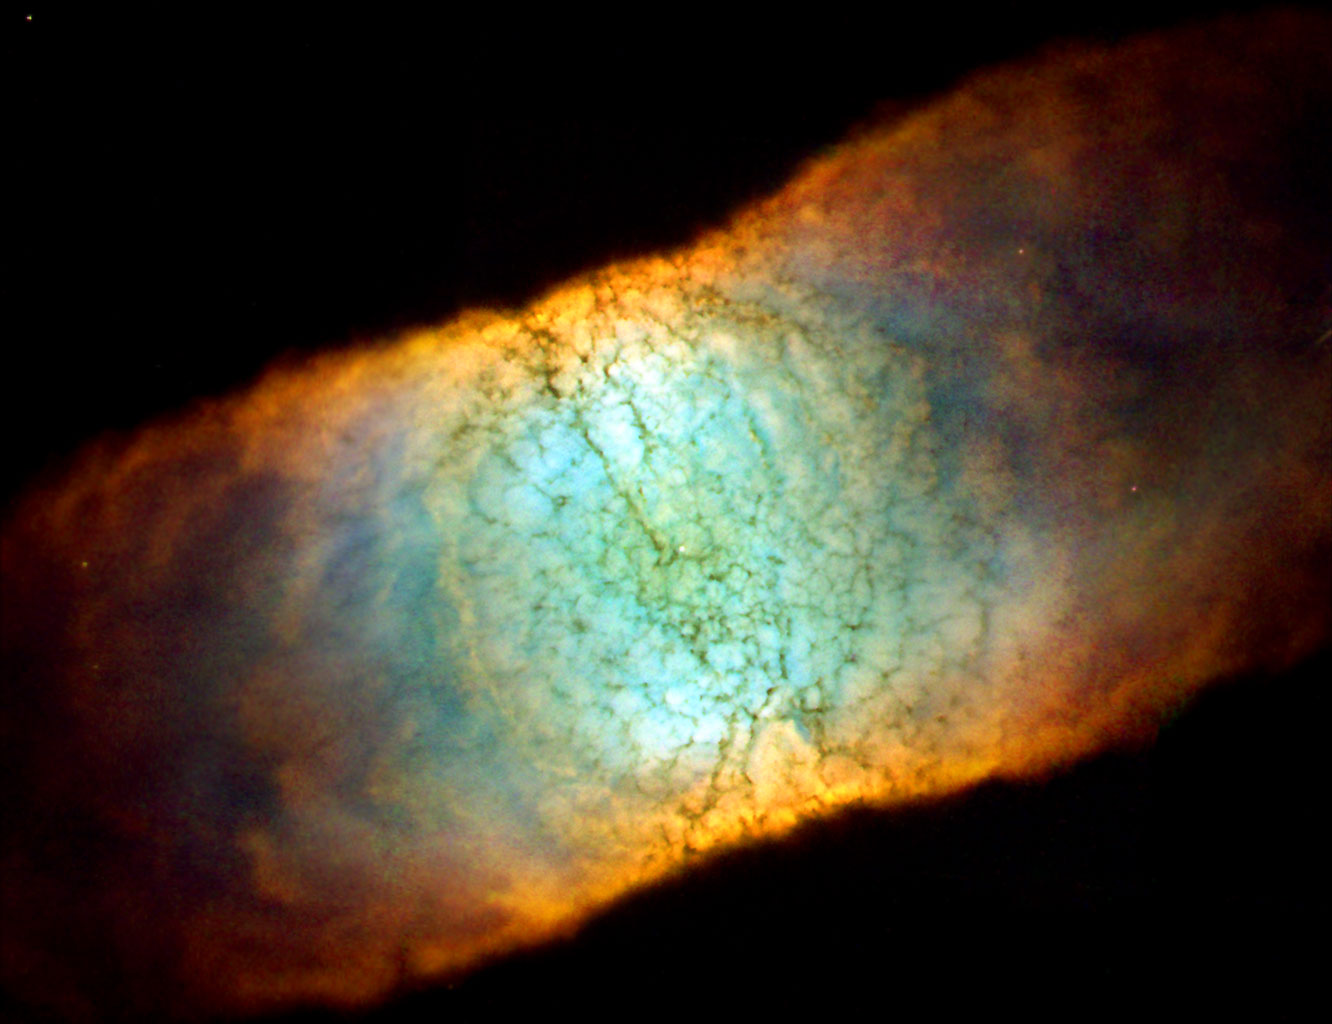
\includegraphics[max width=0.65\linewidth]{../images/retina_nebula.jpg}\]

\begin{enumerate}
\def\labelenumi{\arabic{enumi})}
\tightlist
\item
  ``Retina Nebula'', Hubble Heritage Project,
  \texttt{http://heritage.stsci.edu/2002/14/}
\end{enumerate}

This is actually a tube of ionized gas about a quarter of a light-year
across and one light-year long. It's a planetary nebula produced by a
dying star. If you zoom in and look closely, you can see this star
lurking in the middle, now a mere white dwarf.

The blue light is the most energetic, so it's really hot where you see
blue. This blue light comes from singly ionized helium --- helium where
one electron has been knocked off. The green light is a bit less
energetic: that's from doubly ionized oxygen. The red light comes from
even cooler regions: that's from singly ionized nitrogen.

You can also see a lot of ``dust lanes'' in this photo. They're
beautiful. And they're big! The width of each one is about 160 times the
distance between the Sun and the Earth. The gas and dust in these lanes
is about 1000 times higher than elsewhere. But what creates them?

Apparently, when the fast-moving glowing hot gas from the star crashes
into the invisible gas in the surrounding interstellar space, the
boundary gets sort of crumpled, and these dust lanes form. It's vaguely
similar to the puffy surface of a cumulus cloud. But here the mechanism
is different, because it involves a ``shock wave'': the hot gas is
moving faster than the speed of sound as it hits the cold gas!

This effect is called a ``Vishniac instability'', since in 1983, the
astrophysicist Ethan Vishniac showed that a shock wave moving in a
sufficiently compressible medium would be subject to an instability of
this sort, growing as the square root of time. I've never seen how
Vishniac's calculations work, so the mathematics underlying this
beautiful phenomenon will have to wait for another day.

Note that this planetary nebula, like the others I've shown you, is far
from spherically symmetric. Astrophysicists used to pretend stars were
spherically symmetric. But, that's a bad approximation whenever anything
really exciting happens\ldots{} just like in the
\href{http://en.wikipedia.org/wiki/Spherical_cow}{old joke} where the
punchline is ``consider a spherical cow''.

As I said, the Retina Nebula is actually shaped like a tube. Viewed from
either end, this tube would look very different --- probably like the
Ring Nebula:
\[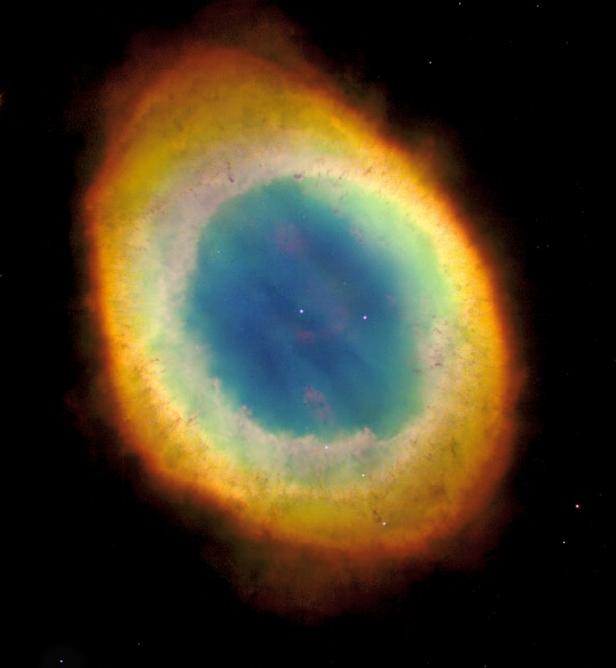
\includegraphics[max width=0.65\linewidth]{../images/ring_nebula.jpg}\]

\begin{enumerate}
\def\labelenumi{\arabic{enumi})}
\setcounter{enumi}{1}
\tightlist
\item
  ``Ring Nebula'', Hubble Heritage Project,
  \texttt{http://heritage.stsci.edu/1999/01/}
\end{enumerate}

This is one light-year across. Again we see He II blue light with a
wavelength of 4686 angstroms, then O III green light at 5007 angstroms,
then N II red light at 6584 angstroms. You can also see the white dwarf
as a tiny dot in the center; it's about 100,000 kelvin in temperature.

(In case you're wondering, an ``angstrom'' is an obsolete but popular
unit of distance, equal to 10\textsuperscript{-10} meters. Just like the
``parsec'', it's a sign that astronomy is an old science. Anders Jonas
Ångström was one of the founders of spectroscopy, back around 1860.
Archaic conventions may also explain why singly ionized helium is called
``He II'', and so on. Maybe the number zero hadn't fully caught on.)

Next: free books!

At least around here, Christmas seems to be all about buying stuff and
giving it away. Giving is good. But I think gifts have more soul if you
make them yourself. This is one of the great things about the internet:
it lets us create things and give them to \emph{everyone in the world}
--- or more precisely: everybody who wants them, and nobody who doesn't.

In this spirit, here's a roundup of free books on math and physics:
gifts from their authors to you. There are lots out there. I'll only
list a few. For more, try these sites:

\begin{enumerate}
\def\labelenumi{\arabic{enumi})}
\setcounter{enumi}{2}
\item
  George Cain, ``Online Mathematics Textbooks'',
  \texttt{http://www.math.gatech.edu/\textasciitilde{}cain/textbooks/onlinebooks.html}
\item
  ``Free Online Mathematics Books'',
  \texttt{http://www.pspxworld.com/book/mathematics/}
\item
  Alex Stefanov, ``Textbooks in Mathematics'',
  \texttt{http://users.ictp.it/\textasciitilde{}stefanov/mylist.html} or
  (with annoying ads, but more permanent)
  \texttt{http://us.geocities.com/alex\_stef/mylist.html}
\end{enumerate}

Despite its title, Stefanov's excellent site includes a lot of books on
physics. I can't find lists \emph{specifically} devoted to free physics
books, but there are a lot out there --- including a lot on the arXiv.

Anyway, let's dive in!

What if you're dying to learn physics, but don't know where to start?
Start here:

\begin{enumerate}
\def\labelenumi{\arabic{enumi})}
\setcounter{enumi}{5}
\tightlist
\item
  ``Physics Books Online'',
  \texttt{http://www.sciencebooksonline.info/physics.html}.
\end{enumerate}

You'll find plenty of free online books, starting from the basics and
working up to advanced topics. But to dig deeper into these mysteries,
you'll eventually need to learn a bunch of math. Do you remember what
\href{http://globetrotter.berkeley.edu/conversations/Weisskopf/}{Victor
Weisskopf} said when a student asked how much math a physicist needs to
know?

``More.''

This can be scary when you're just getting started. What if you don't
know calculus, for example?

Simple: learn calculus! This book is a classic --- and it's free:

\begin{enumerate}
\def\labelenumi{\arabic{enumi})}
\setcounter{enumi}{6}
\tightlist
\item
  Gilbert Strang, \emph{Calculus}, Wellesley-Cambridge Press, Cambridge,
  1991. Also available at
  \texttt{http://ocw.mit.edu/ans7870/resources/Strang/strangtext.htm}
\end{enumerate}

It really explains things clearly. I may use it the next time I teach
calculus. We professors need to quit making our students buy expensive
textbooks, and switch to free online books! We could join forces and
make wiki textbooks that are a lot better and more flexible than the
budget-busting, back-breaking mammoths we currently inflict on our kids.
But there are already a lot of good texts available free online.

Or: what if you know calculus, but you're still swimming through the
undergraduate sea of differential equations, Fourier transforms,
matrices, vectors and tensors? Then this should be really helpful:

\begin{enumerate}
\def\labelenumi{\arabic{enumi})}
\setcounter{enumi}{7}
\tightlist
\item
  James Nearing, \emph{Mathematical Tools for Physics}, available at
  \texttt{http://www.physics.miami.edu/\textasciitilde{}nearing/mathmethods/}
\end{enumerate}

Unlike the usual dry and formal textbook, it reads like a friendly uncle
explaining things in plain English, trying to cut through the red tape
and tell you how to actually think about this stuff.

For example, on page 3 he introduces the hyperbolic trig functions:

\begin{quote}
Where do hyperbolic functions come from? If you have a mass in
equilibrium, the total force on it is zero. If it's in \emph{stable}
equilibrium then if you push it a little to one side and release it, the
force will push it back to the center. If it is \emph{unstable} then
when it's a bit to one side it will be pushed farther away from the
equilibrium point. In the first case, it will oscillate about the
equilibrium position and the function of time will be a circular
trigonometric function --- the common sines or cosines of time,
\(A\cos(\omega t)\). If the point is unstable, the motion will be
described by hyperbolic functions of time, \(\sinh(\omega t)\) instead
of \(\sin(\omega t)\). An ordinary ruler held at one end will swing back
and forth, but if you try to balance it at the other end it will fall
over. That's the difference between \(\cos\) and \(\cosh\).
\end{quote}

He goes into more detail later, after introducing the complex numbers.
This book also features some great animations of Taylor series and
Fourier series, like
\href{http://www.physics.miami.edu/~nearing/mathmethods/power-sine-series.gif}{this
movie of the Taylor series of the sine function}.

There are free online books at all levels\ldots{} so let's soar a bit
higher. How about if you're a more advanced student trying to learn
general relativity? Here you go:

\begin{enumerate}
\def\labelenumi{\arabic{enumi})}
\setcounter{enumi}{8}
\tightlist
\item
  Sean M. Carroll, \emph{Lecture Notes on General Relativity}, available
  as \href{http://arXiv.org/abs/gr-qc/9712019}{\texttt{gr-qc/9712019}}
\end{enumerate}

How about quantum field theory? Then you're in luck --- there are
\emph{two} detailed books available online:

\begin{enumerate}
\def\labelenumi{\arabic{enumi})}
\setcounter{enumi}{9}
\item
  Warren Siegel, \emph{Fields}, available as
  \href{http://arXiv.org/abs/hep-th/9912205}{\texttt{hep-th/9912205}}
\item
  Mark Srednicki, \emph{Quantum Field Theory}, Cambridge U. Press,
  Cambridge, 2007. Also available at
  \texttt{http://www.physics.ucsb.edu/\textasciitilde{}mark/qft.html}
\end{enumerate}

Or what about algebraic topology? Again you're in luck, since you can
read both Allen Hatcher's gentle introduction and Peter May's
high-powered ``concise course'':

\begin{enumerate}
\def\labelenumi{\arabic{enumi})}
\setcounter{enumi}{10}
\item
  Allen Hatcher, \emph{Algebraic Topology}, Cambridge U. Press,
  Cambridge, 2002. Also available at
  \texttt{http://www.math.cornell.edu/\textasciitilde{}hatcher/AT/ATpage.html}
\item
  Peter May, \emph{A Concise Course in Algebraic Topology}, U. of
  Chicago Press, Chicago, 1999. Also available at
  \texttt{http://www.math.uchicago.edu/\textasciitilde{}may/CONCISE/ConciseRevised.pdf}
\end{enumerate}

May has a lot of more advanced topology books available at his website,
too --- like this classic, where he used operads to solve important
problems involving loop spaces:

\begin{enumerate}
\def\labelenumi{\arabic{enumi})}
\setcounter{enumi}{12}
\tightlist
\item
  Peter May, \emph{The Geometry of Iterated Loop Spaces}, Lecture Notes
  in Mathematics \textbf{271}, Springer, Berlin, 1972. Also available at
  \texttt{http://www.math.uchicago.edu/\textasciitilde{}may/BOOKS/gils.pdf}
\end{enumerate}

Or say you want to learn about vector bundles and how they show up in
physics, from the basics all the way to fancy stuff like D-branes and
K-theory? Try this --- it's a great sequel to Husemoller's classic intro
to fiber bundles:

\begin{enumerate}
\def\labelenumi{\arabic{enumi})}
\setcounter{enumi}{13}
\tightlist
\item
  Dale Husemoller, Michael Joachim, Branislav Jurco and Martin
  Schottenloher, \emph{Basic Bundle Theory and K-Cohomology Invariants},
  Lecture Notes in Physics \textbf{726}, Springer, Berlin, 2008. Also
  available at
  \texttt{http://www.mathematik.uni-muenchen.de/\textasciitilde{}schotten\ Texte/978-3-540-74955-4\_Book\_LNP726.pdf}
\end{enumerate}

The list goes on and on! The American Mathematical Society will give you
books for free if you prove that you're not a robot by solving a little
puzzle:

\begin{enumerate}
\def\labelenumi{\arabic{enumi})}
\setcounter{enumi}{14}
\tightlist
\item
  American Mathematical Society, ``Books Online By Subject'',
  \texttt{http://www.ams.org/online\_bks/online\_subject.html}
\end{enumerate}

Apparently they don't want robots learning advanced math and putting us
professors out of business by teaching with more charisma and flair. (By
the way: make sure to let them put cookies on your web browser, or
they'll send you an endless succession of these puzzles, without
explaining why!)

Since James Dolan and I plan to explain symmetric groups and their Hecke
algebras in our online seminar, this particular book from the AMS caught
my eye:

\begin{enumerate}
\def\labelenumi{\arabic{enumi})}
\setcounter{enumi}{15}
\tightlist
\item
  David M. Goldschmidt, \emph{Group Characters, Symmetric Functions, and
  the Hecke Algebra}, AMS, Providence, Rhode Island, 1993. Also
  available as \texttt{http://www.ams.org/online\_bks/ulect4/}
\end{enumerate}

Since we're also struggling to understand the Langlands program, this
looks good too:

\begin{enumerate}
\def\labelenumi{\arabic{enumi})}
\setcounter{enumi}{16}
\tightlist
\item
  Armand Borel, \emph{Automorphic Forms, Representations, and
  \(L\)-functions}, AMS, 2 volumes, Providence, Rhode Island, 1979. Also
  available at \texttt{http://www.ams.org/online\_bks/pspum331/} and
  \texttt{http://www.ams.org/online\_bks/pspum332/}
\end{enumerate}

It's a serious collection of expository papers by bigshots like Borel,
Cartier, Deligne, Jacquet, Knapp, Langlands, Lusztig, Tate, Tits,
Zuckerman, and many more.

``Motives'' are the mysterious virtual building blocks that algebraic
varieties are built from. If you're ready to learn about motives --- I'm
not sure I am --- try this:

\begin{enumerate}
\def\labelenumi{\arabic{enumi})}
\setcounter{enumi}{17}
\tightlist
\item
  Marc Levine, \emph{Mixed Motives}, AMS, Providence, Rhode Island,
  1998. Also available at
  \texttt{http://www.ams.org/online\_bks/surv57/}
\end{enumerate}

Or, if you're interested in using category theory to make analysis
clearer and more beautiful, try this:

\begin{enumerate}
\def\labelenumi{\arabic{enumi})}
\setcounter{enumi}{18}
\tightlist
\item
  Andreas Kriegl and Peter W. Michor, \emph{The Convenient Setting of
  Global Analysis}, AMS, Providence, Rhode Island, 1997. Also available
  at \texttt{http://www.ams.org/online\_bks/surv53/}
\end{enumerate}

The focus is on getting and working with a ``convenient category'' of
infinite-dimensional manifolds. The idea of a ``convenient category''
goes back to topology: at some point, people realized they wanted this
property to hold:
\[\mathcal{C}(X \times Y, Z) \cong \mathcal{C}(X, \mathcal{C}(Y, Z))\]
Here \(\mathcal{C}(X,Y)\) is the space of maps from \(X\) to \(Y\). So,
the isomorphism above says that a map from \(X \times Y to Z\) should
correspond to a map from \(X\) to \(\mathcal{C}(Y,Z)\). A category with
this property is called ``cartesian closed''. While it may not be
obvious why, this property is so wonderful that people threw out the
category of topological spaces and continuous maps and replaced it with
a slightly different one, just to get this to hold.

Another sort of ``convenient category'' for differential geometry uses
infinitesimals. Again, you can learn about this in a free book:

\begin{enumerate}
\def\labelenumi{\arabic{enumi})}
\setcounter{enumi}{19}
\tightlist
\item
  Anders Kock, \emph{Synthetic Differential Geometry}, Cambridge U.
  Press, Cambridge, 2006. Also available at
  \texttt{http://home.imf.au.dk/kock/}
\end{enumerate}

This category is not just cartesian closed --- it's a topos!

If you don't know what a topos is, never fear --- more free books are
coming to your rescue:

\begin{enumerate}
\def\labelenumi{\arabic{enumi})}
\setcounter{enumi}{20}
\item
  Robert Goldblatt, \emph{Topoi, the Categorial Analysis of Logic},
  Dover, 1983. Also available at
  \texttt{http://historical.library.cornell.edu/cgi-bin/cul.math/docviewer?did=Gold010}
\item
  Michael Barr and Charles Wells, \emph{Toposes, Triples and Theories},
  Springer, Berlin, 1983. Also available at
  \texttt{http://www.case.edu/artsci/math/wells/pub/ttt.html}
\end{enumerate}

The first one is so gentle it makes a good introduction to category
theory as a whole. The second scared the bejeezus out of me for a
decade, but now I like it.

I like Jordan algebras, so I was also pleased to see this classic
offered for free at the AMS website:

\begin{enumerate}
\def\labelenumi{\arabic{enumi})}
\setcounter{enumi}{22}
\tightlist
\item
  Nathan Jacobson, \emph{Structure and Representations of Jordan
  Algebras}, AMS, Providence, Rhode Island, 1968. Also available at
  \texttt{http://www.ams.org/online\_bks/coll39/}
\end{enumerate}

Fans of exceptional Lie algebras will like the last two chapters, on
``connections with Lie algebras'' and ``exceptional Jordan algebras''.

Speaking of Lie algebras, I'd never seen this textbook before:

\begin{enumerate}
\def\labelenumi{\arabic{enumi})}
\setcounter{enumi}{23}
\tightlist
\item
  Shlomo Sternberg, \emph{Lie Algebras},
  \texttt{http://www.math.harvard.edu/\textasciitilde{}shlomo/docs/lie\_algebras.pdf}
\end{enumerate}

It's a somewhat quirky introduction, not for beginners I think, but it
features some nice special topics: character formulas, the Kostant Dirac
operator, and a detailed study of the center of the universal enveloping
algebra.

This intro to Lie groups is also a bit quirky, but if you like Feynman
diagrams or spin networks, it's irreplaceable:

\begin{enumerate}
\def\labelenumi{\arabic{enumi})}
\setcounter{enumi}{24}
\tightlist
\item
  Predrag Cvitanovic, \emph{Birdtracks, Lie's, and Exceptional Groups},
  available at \texttt{http://www.nbi.dk/GroupTheory/}
\end{enumerate}

One of the great things about this book is that it classifies simple Lie
groups according to their ``skein relations'' --- properties of their
representations, written out diagrammatically. In so doing, Cvitanovic
realized that there's a ``magic triangle'' containing all the
exceptional Lie groups. This subsumes the ``magic square'' of
Freudenthal and Tits, which I discussed in
\protect\hyperlink{week145}{``Week 145''} and my
\href{http://math.ucr.edu/home/baez/octonions/node16.html}{octonion
webpages}.

This idea of Cvitanovic is closely related to the ``exceptional series''
of Lie groups --- a pattern whose existence was conjectured by Deligne.
I love the term ``exceptional series''. It's an oxymoron, since the
exceptional groups were defined as those that don't fit into any series.
But, it makes sense!

To see the exceptional series, it helps to do a mental backflip called
``Tannaka-Krein duality'', where you focus on the category of
representations of the Lie group, instead of the group itself. Then,
draw the morphisms in that category as diagrams, like Feynman diagrams!
Then see what identities they satisfy. New patterns leap out: new series
unify what had been ``exceptions''.

Very briefly, the idea goes like this. Suppose we have a Lie group \(G\)
with Lie algebra \(L\). The Lie bracket takes two elements \(x\) and
\(y\) and spits out one element \([x,y]\), and it's linear in each
variable, so it gives a linear operator \[L \otimes L \to L\] which is
actually a morphism in the category of representations of \(G\).

So, following the philosophy of Feynman diagrams, we can draw the
bracket operation like this: \[
  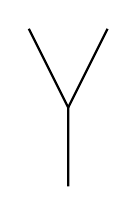
\begin{tikzpicture}
    \draw[thick] (0,0) to (0.5,-1) to (0.5,-2);
    \draw[thick] (1,0) to (0.5,-1);
  \end{tikzpicture}
\] We can even use this to state the definition of a Lie algebra using
diagrams! To say the bracket is antisymmetric: \[[y,x] = -[x,y]\] we
just draw this: \[
  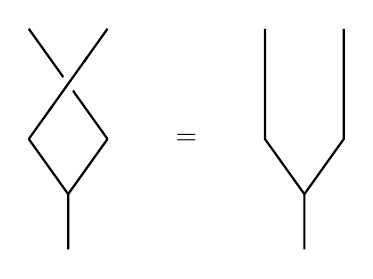
\begin{tikzpicture}[yscale=0.7]
    \begin{knot}[clip width=7]
      \strand[thick] (1,2) to (0,0);
      \strand[thick] (0,2) to (1,0);
    \end{knot}
    \draw[thick] (0,0) to (0.5,-1) to (0.5,-2);
    \draw[thick] (1,0) to (0.5,-1);
    \node at (2,0) {$=$};
    \begin{scope}[shift={(3,0)}]
      \draw[thick] (0,2) to (0,0) to (0.5,-1) to (0.5,-2);
      \draw[thick] (1,2) to (1,0) to (0.5,-1);
    \end{scope}
  \end{tikzpicture}
\]

To say the Jacobi identity: \[[x,[y,z]] = [[x,y],z] + [y,[x,z]]\] we
just draw this: \[
  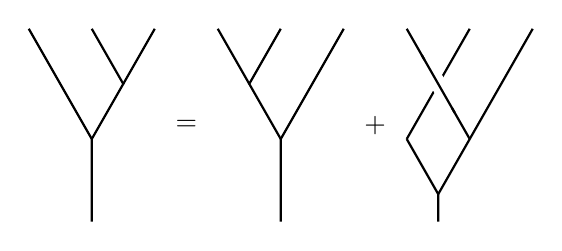
\begin{tikzpicture}[xscale=0.8,yscale=0.7]
    \begin{scope}
      \draw[thick] (0,0) to (1,-2) to (1,-3.5);
      \draw[thick] (1,0) to (1.5,-1) to (1,-2);
      \draw[thick] (2,0) to (1.5,-1);
    \end{scope}
    \node at (2.5,-1.75) {$=$};
    \begin{scope}[shift={(5,0)},xscale=-1]
      \draw[thick] (0,0) to (1,-2) to (1,-3.5);
      \draw[thick] (1,0) to (1.5,-1) to (1,-2);
      \draw[thick] (2,0) to (1.5,-1);
    \end{scope}
    \node at (5.5,-1.75) {$+$};
    \begin{scope}[shift={(6,0)}]
      \begin{knot}[clip width=7]
        \strand[thick] (0,0) to (1,-2);
        \strand[thick] (1,0) to (0,-2);
      \end{knot}
      \draw[thick] (0,-2) to (0.5,-3) to (0.5,-3.5);
      \draw[thick] (2,0) to (0.5,-3);
    \end{scope}
  \end{tikzpicture}
\] If that's too cryptic, maybe this will explain what I'm doing: \[
  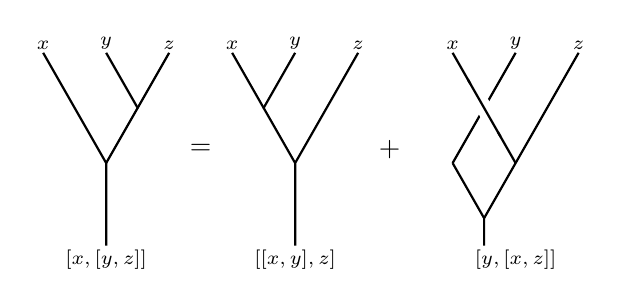
\begin{tikzpicture}[xscale=0.8,yscale=0.7]
    \begin{scope}
      \draw[thick] (0,0) to (1,-2) to (1,-3.5);
      \draw[thick] (1,0) to (1.5,-1) to (1,-2);
      \draw[thick] (2,0) to (1.5,-1);
      \node[label={[label distance=-2mm]above:{\scriptsize$x$}}] at (0,0) {};
      \node[label={[label distance=-2mm]above:{\scriptsize$y$}}] at (1,0) {};
      \node[label={[label distance=-2mm]above:{\scriptsize$z$}}] at (2,0) {};
      \node[label={[label distance=-2mm]below:{\scriptsize$[x,[y,z]]$}}] at (1,-3.5) {};
    \end{scope}
    \node at (2.5,-1.75) {$=$};
    \begin{scope}[shift={(5,0)},xscale=-1]
      \draw[thick] (0,0) to (1,-2) to (1,-3.5);
      \draw[thick] (1,0) to (1.5,-1) to (1,-2);
      \draw[thick] (2,0) to (1.5,-1);
      \node[label={[label distance=-2mm]above:{\scriptsize$z$}}] at (0,0) {};
      \node[label={[label distance=-2mm]above:{\scriptsize$y$}}] at (1,0) {};
      \node[label={[label distance=-2mm]above:{\scriptsize$x$}}] at (2,0) {};
      \node[label={[label distance=-2mm]below:{\scriptsize$[[x,y],z]$}}] at (1,-3.5) {};
    \end{scope}
    \node at (5.5,-1.75) {$+$};
    \begin{scope}[shift={(6.5,0)}]
      \begin{knot}[clip width=7]
        \strand[thick] (0,0) to (1,-2);
        \strand[thick] (1,0) to (0,-2);
      \end{knot}
      \draw[thick] (0,-2) to (0.5,-3) to (0.5,-3.5);
      \draw[thick] (2,0) to (0.5,-3);
      \node[label={[label distance=-2mm]above:{\scriptsize$x$}}] at (0,0) {};
      \node[label={[label distance=-2mm]above:{\scriptsize$y$}}] at (1,0) {};
      \node[label={[label distance=-2mm]above:{\scriptsize$z$}}] at (2,0) {};
      \node[label={[label distance=-2mm]below:{\scriptsize$[y,[x,z]]$}}] at (1,-3.5) {};
    \end{scope}
  \end{tikzpicture}
\] But in fact, people usually massage this picture to make it even more
cryptic, and call it the ``IHX'' identity --- since the three terms look
like the letters I, H, and X by the time they're done twisting them
around. For a good explanation, with pretty pictures, see:

\begin{enumerate}
\def\labelenumi{\arabic{enumi})}
\setcounter{enumi}{25}
\tightlist
\item
  Greg Muller, ``Chord diagrams and Lie algebras'',
  \texttt{http://cornellmath.wordpress.com/2007/12/25/chord-diagrams-and-lie-algebras/}
\end{enumerate}

It then turns out that the exceptional Lie algebras \(\mathrm{F}_4\),
\(\mathrm{E}_6\), \(\mathrm{E}_7\) and \(\mathrm{E}_8\) satisfy
\emph{yet another} identity: \[
  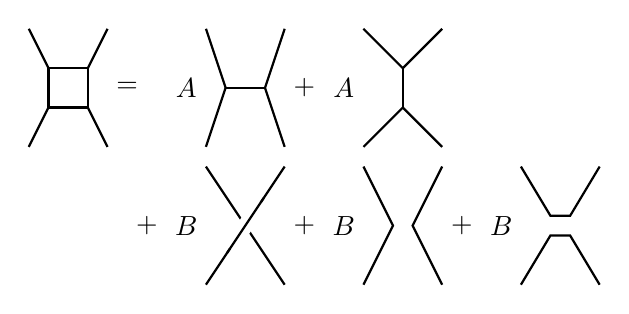
\begin{tikzpicture}[scale=0.5]
    \begin{scope}
      \draw[thick] (0,0) to (0.5,-1);
      \draw[thick] (2,0) to (1.5,-1);
      \draw[thick] (0.5,-2) rectangle ++(1,1);
      \draw[thick] (0.5,-2) to (0,-3);
      \draw[thick] (1.5,-2) to (2,-3);
    \end{scope}
    \node at (2.5,-1.5) {$=$};
    \begin{scope}[shift={(4.5,0)}]
      \node at (-0.5,-1.5) {$A$};
      \draw[thick] (0,0) to (0.5,-1.5);
      \draw[thick] (2,0) to (1.5,-1.5);
      \draw[thick] (0.5,-1.5) to (1.5,-1.5);
      \draw[thick] (0.5,-1.5) to (0,-3);
      \draw[thick] (1.5,-1.5) to (2,-3);
    \end{scope}
    \node at (7,-1.5) {$+$};
    \begin{scope}[shift={(8.5,0)}]
      \node at (-0.5,-1.5) {$A$};
      \draw[thick] (0,0) to (1,-1);
      \draw[thick] (2,0) to (1,-1);
      \draw[thick] (1,-1) to (1,-2);
      \draw[thick] (1,-2) to (0,-3);
      \draw[thick] (1,-2) to (2,-3);
    \end{scope}
    \node at (3,-5) {$+$};
    \begin{scope}[shift={(4.5,-3.5)}]
      \node at (-0.5,-1.5) {$B$};
      \begin{knot}[clip width=7]
        \strand[thick] (2,0) to (0,-3);
        \strand[thick] (0,0) to (2,-3);
      \end{knot}
    \end{scope}
    \node at (7,-5) {$+$};
    \begin{scope}[shift={(8.5,-3.5)}]
      \node at (-0.5,-1.5) {$B$};
      \draw[thick] (0,0) to (0.75,-1.5) to (0,-3);
      \draw[thick] (2,0) to (1.25,-1.5) to (2,-3);
    \end{scope}
    \node at (11,-5) {$+$};
    \begin{scope}[shift={(12.5,-3.5)}]
      \node at (-0.5,-1.5) {$B$};
      \draw[thick] (0,0) to (0.75,-1.25) to (1.25,-1.25) to (2,0);
      \draw[thick] (0,-3) to (0.75,-1.75) to (1.25,-1.75) to (2,-3);
    \end{scope}
  \end{tikzpicture}
\] for various choices of the constants \(A\) and \(B\). So, they fit
into a ``series''!

I believe the main point of this identity, going back to Vogel's paper
``Algebraic structures on modules of diagrams'', is that for these Lie
algebras, the square of the quadratic Casimir is the only degree-4
Casimir.

I think there's a lot more to be discovered here, in part by taking the
gnarly computations people have done so far and making them more
beautiful and conceptual. So, I urge all fans of exceptional
mathematics, diagrams, and categories to look at these:

\begin{enumerate}
\def\labelenumi{\arabic{enumi})}
\setcounter{enumi}{26}
\item
  Pierre Deligne, ``La serie exceptionnelle des groupes de Lie'',
  \emph{C. R. Acad. Sci. Paris Ser. I Math} \textbf{322} (1996),
  321--326.

  Pierre Deligne and R. de Man, ``The exceptional series of Lie groups
  II'', \emph{C. R. Acad. Sci. Paris Ser. I Math} \textbf{323} (1996),
  577--582.

  Pierre Deligne and Benedict Gross, ``On the exceptional series, and
  its descendants'', \emph{C. R. Acad. Sci. Paris Ser. I Math}
  \textbf{335} (2002), 877--881. Also available as
  \texttt{http://www.math.ias.edu/\textasciitilde{}phares/deligne/ExcepSeries.ps}
\item
  Pierre Vogel, ``Algebraic structures on modules of diagrams'', 1995.
  Available at
  \texttt{http://www.institut.math.jussieu.fr/\textasciitilde{}vogel/}
  or \texttt{http://citeseer.ist.psu.edu/469395.html}

  ``The universal Lie algebra'', 1999. Available at
  \texttt{http://www.institut.math.jussieu.fr/\textasciitilde{}vogel/}

  ``Vassiliev theory and the universal Lie algebra'', 2000. Available at
  \texttt{http://www.institut.math.jussieu.fr/\textasciitilde{}vogel/}
\end{enumerate}

For a good overview, try this:

\begin{enumerate}
\def\labelenumi{\arabic{enumi})}
\setcounter{enumi}{27}
\tightlist
\item
  J. M. Landsberg and L. Manivel, ``Representation theory and projective
  geometry'', 2002. Available at
  \href{http://arXiv.org/abs/math/0203260}{\texttt{arXiv:math/0203260}}.
\end{enumerate}

Alas, they avoid drawing Feynman diagrams, though they talk about them
in section 4. They prefer to use ideas from algebraic geometry:

\begin{enumerate}
\def\labelenumi{\arabic{enumi})}
\setcounter{enumi}{28}
\item
  J. M. Landsberg and L. Manivel, ``The projective geometry of
  Freudenthal's magic square'', \emph{J. Algebra} \textbf{239} (2001),
  477--512. Also available as
  \href{http://arXiv.org/abs/math/9908039}{\texttt{arXiv:math/9908039}}.

  J. M. Landsberg and L. Manivel, ``Triality, exceptional Lie algebras
  and Deligne dimension formulas'', \emph{Adv. Math.} \textbf{171}
  (2002), 59--85. Also available as
  \href{http://arXiv.org/abs/math/0107032}{\texttt{arXiv:math/0107032}}.

  J. M. Landsberg and L. Manivel, ``Series of Lie groups'', available as
  \href{http://arXiv.org/abs/math/0203241}{\texttt{arXiv:math/0203241}}.
\end{enumerate}

Bruce Westbury, whom longtime readers of This Week's Finds will remember
as John Barrett's collaborator, has also worked on this subject. He has
pointed out that both the magic square and the magic triangle can be
given an extra row and column if we introduce a \(6\)-dimensional
algebra halfway between the quaternions and the octonions:

\begin{enumerate}
\def\labelenumi{\arabic{enumi})}
\setcounter{enumi}{29}
\tightlist
\item
  Bruce Westbury, ``Sextonions and the magic square'', available as
  \href{http://arXiv.org/abs/math/0411428}{\texttt{arXiv:math/0411428}}.
\end{enumerate}

For even more references, try this:

\begin{enumerate}
\def\labelenumi{\arabic{enumi})}
\setcounter{enumi}{30}
\tightlist
\item
  Bruce Westbury, ``References on series of Lie groups'',
  \texttt{http://www.mpim-bonn.mpg.de/digitalAssets/2763\_references.pdf}
\end{enumerate}

This stuff has been on my mind recently, since I've been working on
exceptional groups and grand unified theories with my student John
Huerta. Also, my friend Tevian Dray has a student who just finished a
thesis on a related topic:

\begin{enumerate}
\def\labelenumi{\arabic{enumi})}
\setcounter{enumi}{31}
\tightlist
\item
  Aaron Wangberg, ``The structure of \(\mathrm{E}_6\)'', available as
  \href{http://arXiv.org/abs/0711.3447}{\texttt{arXiv:0711.3447}}.
\end{enumerate}

In a nutshell: \(\mathrm{E}_6\) is secretly
\(\mathrm{SL}(3,\mathbb{O})\). Octonions rock!

Happy holidays. Keep learning cool stuff.

\begin{center}\rule{0.5\linewidth}{0.5pt}\end{center}

\textbf{Addenda:} Thomas Riepe listed some more free online math books.
Tony Smith pointed out something I already knew, but didn't make clear
above: the idea that \(\mathrm{E}_6\) is secretly
\(\mathrm{SL}(3,\mathbb{O})\) is far from new.

Thomas wrote:

\begin{quote}
Some more links:

\begin{itemize}
\tightlist
\item
  Milne's \href{http://www.jmilne.org/math/index.html}{great collection}
  (incl.~the famous LNM 900), leading the reader from basic algebra
  through algebraic number theory, class fields, modular forms,
  arithmetic groups,\ldots{} up to etale cohomology, Shimura varieties
  etc.
\item
  \href{http://www.math.uni-bielefeld.de/~fw/}{Friedhelm Waldhausen's
  lectures} on algebraic topology and K-theory.
\item
  \href{http://www.mathematik.uni-bielefeld.de/~rehmann/DML/dml_links_author_A.html}{DML:
  Digital Mathematics Library}
\item
  \href{http://www.math.uni-bonn.de/people/harder/}{G. Harder's
  math-links}
\item
  \href{http://www.msri.org/publications/books/}{MSRI online books}
\end{itemize}

Finally:

\begin{quote}
``Nearly three and a half centuries of scientific study and achievement
is now available online in the
\href{http://www.pubs.royalsoc.ac.uk/archive}{Royal Society Journals
Digital Archive}. This is the longest-running and arguably most
influential journal archive in Science, including all the back articles
of both Philosophical Transactions and Proceedings.''
\end{quote}
\end{quote}

Tony Smith wrote:

\begin{quote}
Thanks for an interesting list of stuff in week 260, but I have some
questions about this:

\begin{quote}
\begin{enumerate}
\def\labelenumi{\arabic{enumi})}
\setcounter{enumi}{31}
\tightlist
\item
  Aaron Wangberg, ``The structure of \(\mathrm{E}_6\)'', available as
  \href{http://www.arxiv.org/abs/0711.3447}{\texttt{arXiv:0711.3447}}.
\end{enumerate}

In a nutshell: \(\mathrm{E}_6\) is secretly
\(\mathrm{SL}(3,\mathbb{O})\). Octonions rock!
\end{quote}

Not only from your brief list descrption, but also from reading the
paper at pages 96 ff I get the impression that Wangberg is claiming the
result \(\mathrm{E}_6 = \mathrm{SL}(3,\mathbb{O})\). Do you get the same
impression? I hope not, and I hope that my impression is somehow
mistaken, because the result
\(\mathrm{E}_6 = \mathrm{SL}(3,\mathbb{O})\) is (and has been for some
time) well known and in the literature. For example, in
\href{http://arxiv.org/abs/hep-th/9309030}{\texttt{hep-th/9309030}}
Martin Cederwall and Christian R. Preitschopf said:

\begin{quote}
\ldots{} It should be possible to realize
\(\mathrm{E}_6 = \mathrm{SL}(3;\mathbb{O})\) {[}18,24{]} on them in a
``spinor-like'' manner, much like
\(\mathrm{SO}(10) = \mathrm{SL}(2;\mathbb{O})\) acts on its
\(16\)-dimensional spinor representations that play the role of
homogeneous coordinates for \(\mathbb{OP}^1\) \ldots{}

\ldots{}\\
18. H. Freudenthal, \emph{Adv. Math.} \textbf{1} (1964) 145.\\
\ldots{}\\
24. A. Sudbery, \emph{J. Phys.} \textbf{A17} (1984) 939. \ldots.\\
\end{quote}

Although that Freudenthal Adv. Math. is listed as a reference in
Wangberg's paper (as reference 5), I did not see the Sudbery paper
listed, and I did not see the Freudenthal reference on page 96.

Please don't misunderstand this message. I think that Wangberg's thesis
is very interesting. I am just trying to get a correct historical
record.

Tony

PS --- In Sudbery's 1984 paper, he not only says (at page 950)
``\ldots{} \(\mathfrak{sl}(3,\mathbb{K})\) \ldots{} When
\(\mathbb{K} = \mathbb{O}\), this Lie algebra is a non-compact form of
the exceptional Lie algebra \(\mathrm{E}_6\), the maximal compact
subalgebra being \(\mathrm{F}_4\) \ldots{}'' but he goes on to say
``\ldots{} \(\mathfrak{sp}(6,\mathbb{K})\) \ldots{} when
\(\mathbb{K} = \mathbb{O}\) it is a non-compact form of
\(\mathrm{E}_7\), the maximal compact subalgebra being
\(\mathrm{E}_6 \oplus \mathfrak{so}(2)\). \ldots{}''.
\end{quote}

For more discussion, go to the
\href{http://golem.ph.utexas.edu/category/2007/12/this_weeks_finds_in_mathematic_20.html}{\(n\)-Category
Café}.

\begin{center}\rule{0.5\linewidth}{0.5pt}\end{center}

\begin{quote}
\emph{If nature has made any one thing less susceptible than all others
of exclusive property, it is the action of the thinking power called an
idea, which an individual may exclusively possess as long as he keeps it
to himself; but the moment it is divulged, it forces itself into the
possession of every one, and the receiver cannot dispossess himself of
it. Its peculiar character, too, is that no one possesses the less,
because every other possesses the whole of it.}

--- Thomas Jefferson
\end{quote}



\hypertarget{week261}{%
\section{March 19, 2008}\label{week261}}

Sorry for the long pause! I've been busy writing. For example: a gentle
introduction to category theory, focusing on its role as a ``Rosetta
Stone'' that helps us translate between four languages:

\begin{enumerate}
\def\labelenumi{\arabic{enumi})}
\tightlist
\item
  John Baez and Mike Stay, ``Physics, topology, logic and computation: a
  Rosetta Stone'', to appear in \emph{New Structures in Physics},
  ed.~Bob Coecke. Available at
  \texttt{http://math.ucr.edu/home/baez/rosetta.pdf}
\end{enumerate}

The idea is to take this chart and make it really precise:

\begin{longtable}[]{@{}llll@{}}
\toprule
\textbf{Physics} & \textbf{Topology} & \textbf{Logic} &
\textbf{Computation}\tabularnewline
\midrule
\endhead
Hilbert space & manifold & proposition & data type\tabularnewline
operator & cobordism & proof & program\tabularnewline
\bottomrule
\end{longtable}

In each case we have a kind of ``thing'' and a kind of ``process'' going
between things. But it turns out we can make the analogies much sharper
and more detailed than that.

The hard work has already been done by many researchers. People working
on topological quantum field theory have seen how cobordisms ---
spacetimes going from one slice of space to another --- are analogous to
operators between Hilbert spaces. The ``Curry-Howard correspondence''
makes the analogy between proofs and programs precise. Girard's work on
``linear logic'' sets up an analogy between operators and proofs. And so
on\ldots.

We're just trying to present these analogies in an easy-to-read form,
all in one place. I hope that pondering them will help us break down
some walls separating disciplines. In more optimistic moments, I even
thnk they represent the first steps toward a general theory of systems
and processes! Then I remember that scientists are trained to distrust
such grand visions, and for good reasons. Time will tell.

But enough of that. This Week will be an ode to the number 3.

First, though\ldots{} here's the nebula of the week!
\[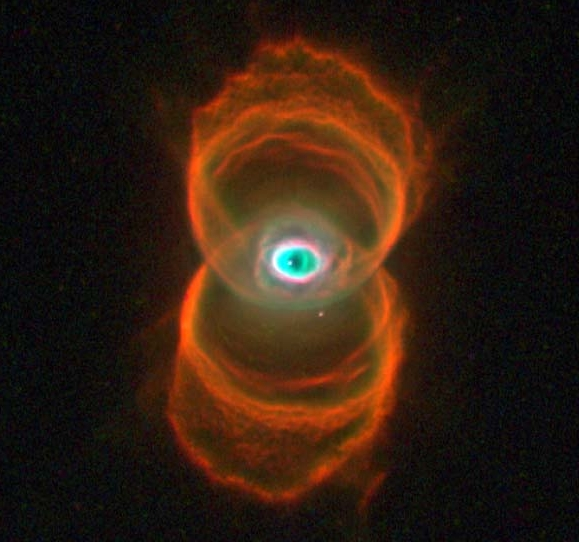
\includegraphics[max width=0.65\linewidth]{../images/hourglass_nebula.jpg}\]

\begin{enumerate}
\def\labelenumi{\arabic{enumi})}
\setcounter{enumi}{1}
\tightlist
\item
  ``Hubble finds an hourglass nebula around a dying star'',
  \texttt{http://hubblesite.org/newscenter/archive/releases/nebula/planetary/1996/07/}
\end{enumerate}

It looks like the eye of Sauron in Tolkien's \emph{Lord of the Rings}
trilogy. It's not. It's a planetary nebula 8000 light years away, called
MyCn 18 --- or, more romantically, the Engraved Hourglass Nebula.

The colors look unreal. They are.

\begin{itemize}
\tightlist
\item
  H\(\alpha\) light is shown as as green, but it's actually red. This is
  the light hydrogen emits when its one electron jumps from its
  \(n = 3\) state to its \(n = 2\) state.
\item
  N II light is shown as red, and it actually is. This is light from
  singly ionized nitrogen.
\item
  O III light is shown as blue, but it's actually green. This is light
  from doubly ionized oxygen.
\item
  Furthermore, the colors have been adjusted so that regions where
  H\(\alpha\) and O II overlap are orange.
\end{itemize}

Okay, so the colors are fake. But how did this weird nebula form? You
can see a clue if you pay attention: the bright white dwarf star isn't
located exactly at the center. It's a bit to the left! This paper,
written by the folks who took the photograph, argues that it has an
unseen companion:

\begin{enumerate}
\def\labelenumi{\arabic{enumi})}
\setcounter{enumi}{2}
\tightlist
\item
  Raghvendra Sahai et al, ``The Etched Hourglass Nebula MyCn 18. I:
  Hubble space telescope observations'', \emph{The Astronomical Journal}
  \textbf{118} (1999), 468--476. Also available at
  \texttt{http://www.iop.org/EJ/article/1538-3881/118/1/468/990080.text.html}
\end{enumerate}

This paper tackles the difficult problem of modelling the nebula:

\begin{enumerate}
\def\labelenumi{\arabic{enumi})}
\setcounter{enumi}{3}
\tightlist
\item
  Raghvendra Sahai et al, ``The Etched Hourglass Nebula MyCn 18. II: A
  spatio-kinematic model'', \emph{The Astronomical Journal} \textbf{110}
  (2000), 315--322. Also available at
  \texttt{http://www.iop.org/EJ/article/1538-3881/119/1/315/990248.text.html}
\end{enumerate}

It doesn't seem that the white dwarf alone could have produced all the
glowing gas we see here. A red giant companion could help. But, there
are lots of mysteries.

That shouldn't be surprising. Even the simplest things can be quite rich
in complexity if you look at them hard enough. I'll illustrate this with
a little ode to the number 3. I'll start off slow, and ramp up to a
discussion of how all these mathematical entities are locked in a tight
embrace:

\begin{itemize}
\tightlist
\item
  the trefoil knot
\item
  cubic polynomials
\item
  the group of permutations of 3 things
\item
  the three-strand braid group
\item
  modular forms and cusp forms
\end{itemize}

As a kind of intermezzo, I'll talk about how to solve the cubic
equation. We all learn about quadratic equations in school: they're the
bread and butter of algebra, right after linear equations. Cubics are
trickier, but studying them can give you a lifetime's worth of fun.

Let's start with the trefoil knot. This is the simplest of knots:
\[\href{http://en.wikipedia.org/wiki/Trefoil_knot}{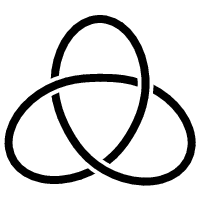
\includegraphics[max width=0.65\linewidth]{../images/TrefoilKnot-01.png}}\]
You can even draw it on the surface of a doughnut! Just take a pen and
draw a curve that winds around your doughnut three time in one direction
as it winds twice in the other direction:
\[\href{http://www.popmath.org.uk/sculpmath/pagesm/torus2.html}{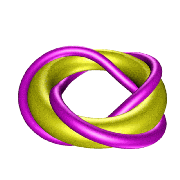
\includegraphics[max width=0.65\linewidth]{../images/tortef2j.png}}\]

\begin{enumerate}
\def\labelenumi{\arabic{enumi})}
\setcounter{enumi}{4}
\tightlist
\item
  Center for the Popularisation of Mathematics, ``Torus knots'',
  \texttt{http://www.popmath.org.uk/sculpmath/pagesm/torus2.html}
\end{enumerate}

Mathematically, the surface of a doughnut is called a ``torus''. We can
describe a point on the torus by two angles running from \(0\) to
\(2\pi\) --- the ``latitude'' and ``longitude''. But another name for
such an angle is a ``point on the unit circle''. If we think of the unit
circle in the complex plane, this gives us a nice equation for the
trefoil: \[u^2 = v^3\] Here \(u\) and \(v\) are complex numbers with
absolute value \(1\). The equation says that as \(u\) moves around the
unit circle, \(v\) moves around \(2/3\) as fast. So, the set of
solutions is a curve on the torus that winds around thrice in one
direction while it winds around twice in the other direction --- a
trefoil knot!

We can also drop the restriction that \(u\) and \(v\) have absolute
value \(1\). Then the equation \(u^2 = v^3\) is famous for other reasons
--- it's related to cubic equations!

As you've probably heard, there's a formula for solving cubic equations,
sort of like the quadratic formula, but bigger and badder. It goes back
to some Italians in the 1500s who liked to challenge each other with
equations and make bets on who could solve them: Scipione del Ferro,
Niccolo Tartaglia and Gerolamo Cardano.

Imagine we're trying to solve a cubic equation. We can always divide by
the coefficient of the cubic term, so it's enough to consider equations
like this: \[z^3 + Az^2 + Bz + C = 0\] If we could solve this and find
the roots \(a\), \(b\), and \(c\), we could write it as:
\[(z - a)(z - b)(z - c) = 0\] But this means \[
  \begin{aligned}
    A &= -(a + b + c)
  \\B &= ab + bc + ca
  \\C &= -abc
  \end{aligned}
\] Note that \(A\), \(B\), and \(C\) don't change when we permute \(a\),
\(b\), and \(c\). So, they're called ``symmetric polynomials'' in the
variables \(a\), \(b\), and \(c\).

You see this directly, but there's also a better explanation: the
coefficients of a polynomial depend on its roots, but they don't change
when we permute the roots.

I can't resist mentioning a cool fact, which is deeply related to the
trefoil: \emph{every} symmetric polynomial of \(a\), \(b\), and \(c\)
can be written as a polynomial in \(A\), \(B\), and \(C\) --- and in a
unique way!

In fact, this sort of thing works not just for cubics, but for
polynomials of any degree. Take a general polynomial of degree \(n\) and
write the coefficients as functions of the roots. Then these functions
are symmetric polynomials, and \emph{every} symmetric polynomial in
\(n\) variables can be written as a polynomial of these --- and in a
unique way.

But, back to our cubic. Note that \(-A/3\) is the average of the three
roots. So, if we slide \(z\) over like this: \[x = z + \frac{A}{3}\] we
get a new cubic equation for which the average of the three roots is
zero. This new cubic equation will be of this form: \[x^3 + Bx + C = 0\]
for some new numbers \(B\) and \(C\). In other words, the ``\(A\)'' in
this new cubic is zero, since we translated the roots to make their
average zero.

So, to solve cubic equations, it's enough to solve cubics like
\(x^3 + Bx + C = 0\). This is a great simplification. When you first see
it, it's really exciting. But then you realize you have no idea what to
do next! This must be why it's called a ``depressed cubic''.

In fact, Scipione del Ferro figured out how to solve the ``depressed
cubic'' shortly after 1500. So, you might think he could solve any
cubic. But, \emph{negative numbers hadn't been invented yet}. This
prevented him from reducing any cubic to a depressed one!

It's sort of hilarious that Ferro was solving cubic equations before
negative numbers were worked out. It should serve as a lesson: we
mathematicians often work on fancy stuff before understanding the
basics. Often that's why math seemss hard! But often it's impossible to
discover the basics except by working on fancy stuff and getting stuck.

Here's one trick for solving the depressed cubic \(x^3 + Bx + C = 0\).
Write \[x = y - \frac{B}{3y}\] Plugging this in the cubic, you'll get a
quadratic equation in \(y^3\), which you can solve. From this you can
figure out \(y\), and then \(x\).

Alas, I have no idea what this trick means. Does anyone know? Ferro and
Tartaglia used a more long-winded method that seems just as sneaky.
Later Lagrange solved the cubic yet another way. I like his way because
it contains strong hints of Galois theory.

You can see all these methods here:

\begin{enumerate}
\def\labelenumi{\arabic{enumi})}
\setcounter{enumi}{5}
\tightlist
\item
  Wikipedia, ``Cubic function'',
  \texttt{http://en.wikipedia.org/wiki/Cubic\_equation}.
\end{enumerate}

So, I won't say more about solving the cubic now. Instead, I want to
explain the ``discriminant''. This is a trick for telling when two roots
of our cubic are equal. It turns out to be related to the trefoil knot.

For a quadratic equation \(ax^2 + bx + c = 0\), the two roots are equal
precisely when \(b^2 - 4ac = 0\). That's why \(b^2 - 4ac\) is called the
``discriminant'' of the quadratic. The same idea works for other
equations; let's see how it goes for the cubic.

Suppose we were smart enough to find the roots of our cubic
\[x^3 + Bx + C = 0\] and write it as \[(x - a)(x - b)(x - c) = 0\] Then
two roots are equal precisely when \[(a - b)(b - c)(c - a) = 0\] The
left side isn't a symmetric polynomial in \(a\), \(b\), and \(c\); it
changes sign whenever we switch two of these variables. But if we square
it, we get a symmetric polynomial that does the same job:
\[D = (a - b)^2 (b - c)^2 (c - a)^2\] This is the discriminant of the
cubic! By what I said about symmetric polynomials, it has to be a
polynomial in \(B\) and \(C\) (since \(A = 0\)). If you sweat a while,
you'll see \[D = -4B^3 - 27C^2\] So, here's the grand picture: we've got
a \(2\)-dimensional space of cubics with coordinates \(B\) and \(C\).
Sitting inside this 2d space is a curve consisting of ``degenerate''
cubics --- cubics with two roots the same. This curve is called the
``discriminant locus'', since it's where the discriminant vanishes:
\[4B^3 + 27C^2 = 0\] If we only consider the case where \(B\) and \(C\)
are real, the discriminant locus looks like this: \[
  \begin{tikzpicture}
    \begin{axis}[
      axis x line=middle,
      axis y line=middle,
      ticks=none,
      xlabel={$B$},
      ylabel={$C$},
      xmin=-1,xmax=1
      ]
      \addplot[thick,domain=-1:1,samples=50] ({-x^2},{x^3});
    \end{axis}
  \end{tikzpicture}
\] It's smooth except at the origin, where it has a sharp point called a
``cusp''.

Now here's where the trefoil knot comes in. The equation for the
discriminant locus: \[4B^3 + 27C^2 = 0\] should remind you of the
equation for the trefoil: \[u^2 = v^3\] Indeed, after a linear change of
variables they're the same! But, for the trefoil we need \(u\) and \(v\)
to be \emph{complex} numbers. We took them to be unit complex numbers,
in fact.

So, the story is this: we've got a \(2\)-dimensional \emph{complex}
space of complex cubics. Sitting inside it is a \emph{complex} curve,
the discriminant locus. In our new variables, it's this: \[u^2 = v^3\]
If we intersect this discriminant locus with the torus \[|u| = |v| = 1\]
we get a trefoil knot. But that's not all!

Normal folks think of knots as living in ordinary 3d space, but
topologists often think of them as living in a \(3\)-sphere: a sphere in
4d space. That's good for us. We can take this 4d space to be our 2d
complex space of complex cubics! We can pick out spheres in this space
by equations like this: \[|u|^2 + |v|^3 = c \qquad \mbox{($c > 0$)}\]
These are not round \(3\)-spheres, thanks to that annoying third power.
But, they're topologically \(3\)-spheres. If we take any one of them and
intersect it with our discriminant locus, we get a trefoil knot! This is
clear when \(c = 2\), since then we have \[|u|^2 + |v|^3 = 2\] and
\[u^2 = v^3\] which together imply \[|u| = |v| = 1\] But if you think
about it, we also get a trefoil knot for any other \(c > 0\). This
trefoil shrinks as \(c \to 0\), and at \(c = 0\) it reduces to a single
point, which is also the cusp here: \[
  \begin{tikzpicture}
    \begin{axis}[
      axis x line=middle,
      axis y line=middle,
      ticks=none,
      xlabel={$v$},
      ylabel={$u$},
      xmin=-1,xmax=1
      ]
      \addplot[thick,domain=-1:1,samples=50] ({x^2},{x^3});
    \end{axis}
  \end{tikzpicture}
\] We don't see trefoil knots in this picture because it's just a real
2d slice of the complex 2d picture. But, they're lurking in the
background!

Now let me say how the group of permutations of three things gets into
the game. We've already seen the three things: they're the roots \(a\),
\(b\), and \(c\) of our depressed cubic! So, they're three points on the
complex plane that add to zero. Being a physicist at heart, I sometimes
imagine them as three equal-mass planets, whose center of mass is at the
origin.

The space of possible positions of these planets is a 2d complex vector
space, since we can use any two of their positions as coordinates and
define the third using the relation \[a + b + c = 0\] So, there are
three coordinate systems we can use: the \((a,b)\) system, the \((b,c)\)
system and the \((c,a)\) system. We can draw all three coordinate
systems at once like this: \[
  \begin{tikzpicture}
    \draw[thick,->] (180:2) to (0:2) node[label=right:{$a$}]{};
    \draw[thick,->] (-60:2) to (120:2) node[label=above left:{$b$}]{};
    \draw[thick,->] (60:2) to (-120:2) node[label=below left:{$c$}]{};
    \node at (0,0) {$\bullet$};
  \end{tikzpicture}
\] The group of permutations of 3 things acts on this picture by
permuting the three axes. Beware: I've only drawn a \(2\)-dimensional
\emph{real} vector space here, just a slice of the full 2d complex
space.

Now suppose we take this 2d complex space and mod out by the permutation
symmetries. What do we get? It turns out we get \emph{another} 2d
complex vector space! In this new space, the three coordinate axes shown
above become just one thing\ldots{} but this thing is a curve, like
this: \[
  \begin{tikzpicture}
    \begin{axis}[
      axis x line=none,
      axis y line=none,
      ticks=none,
      xlabel={},
      ylabel={},
      xmin=-1,xmax=1
      ]
      \addplot[thick,domain=-1:1,samples=50] ({-x^2},{x^3});
    \end{axis}
  \end{tikzpicture}
\] Look familiar? Sure! It's just the discriminant locus we've seen
before.

Why does it work this way? The explanation is sitting before us. We've
got two 2d complex vector spaces: the space of possible \emph{ordered
triples of roots} of a depressed cubic, and the space of possible
\emph{coefficients}. There's a map from the first space to the second,
since the coefficients are functions of the roots: \[
  \begin{aligned}
    B &= ab + bc + ca
  \\C &= -abc
  \end{aligned}
\] These functions are symmetric polynomials: they don't change when we
permute \(a\), \(b\), and \(c\). And, it follows from what I said
earlier that we can get \emph{any} symmetric polynomial as a function of
these --- under the assumption that \(a+b+c = 0\), that is.

So, the map where we mod out by permutation symmetries of the roots is
exactly the map from roots to coefficients.

The lines in this picture are places where two roots are equal: \[
  \begin{tikzpicture}
    \draw[thick,->] (180:2) to (0:2) node[label=right:{$b=c$}]{};
    \draw[thick,->] (-60:2) to (120:2) node[label=above left:{$c=a$}]{};
    \draw[thick,->] (60:2) to (-120:2) node[label=below left:{$a=b$}]{};
    \node at (0,0) {$\bullet$};
  \end{tikzpicture}
\] So, when we apply the map from roots to coefficients, these lines get
mapped to the discriminant locus: \[
  \begin{tikzpicture}
    \begin{axis}[
      axis x line=middle,
      axis y line=middle,
      ticks=none,
      xlabel={},
      ylabel={},
      xmin=-1,xmax=1
      ]
      \addplot[thick,domain=-1:1,samples=50] ({-x^2},{x^3});
    \end{axis}
  \end{tikzpicture}
\]

You should now feel happy and quit reading\ldots{} unless you know a bit
of topology. If you \emph{do} know a little topology, here's a nice
spinoff of what we've done. Though I didn't say it using so much jargon,
we've already seen that space of nondegenerate depressed cubics is
\(\mathbb{C}^2\) minus a cone on the trefoil knot. So, the fundamental
group of this space is the same as the fundamental group of \(S^3\)
minus a trefoil knot. This is a famous group: it has three generators
\(x,y,z\), and three relations saying that:

\begin{itemize}
\tightlist
\item
  \(x\) conjugated by \(y\) is \(z\)
\item
  \(y\) conjugated by \(z\) is \(x\)
\item
  \(z\) conjugated by \(x\) is \(y\)
\end{itemize}

On the other hand, we've seen this space is the space of triples of
distinct points in the plane, centered at the origin, mod permutations.
The condition ``centered at the origin'' doesn't affect the fundamental
group. So, this fundamental group is another famous group: the ``braid
group on 3 strands''. This has two generators: \[
  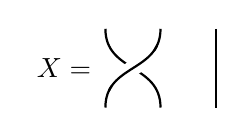
\begin{tikzpicture}[xscale=0.7]
    \node at (-0.75,-0.5) {$X=$};
    \begin{knot}[clip width=7]
      \strand[thick] (1,0)
        to [out=down,in=up] (0,-1);
      \strand[thick] (0,0)
        to [out=down,in=up] (1,-1);
      \strand[thick] (2,0) to (2,-1);
    \end{knot}
  \end{tikzpicture}
  \qquad\qquad
  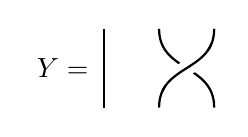
\begin{tikzpicture}[xscale=0.7]
    \node at (-0.75,-0.5) {$Y=$};
    \begin{knot}[clip width=7]
      \strand[thick] (2,0)
        to [out=down,in=up] (1,-1);
      \strand[thick] (1,0)
        to [out=down,in=up] (2,-1);
      \strand[thick] (0,0) to (0,-1);
    \end{knot}
  \end{tikzpicture}
\] and one relation, called the ``Yang-Baxter equation'' or ``third
Reidemeister move'': \[
  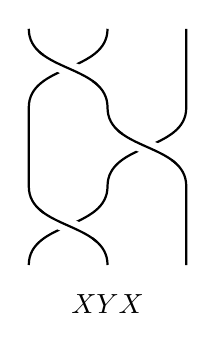
\begin{tikzpicture}
    \begin{knot}[clip width=7]
      \strand[thick] (0,0)
        to [out=down,in=up] (1,-1)
        to [out=down,in=up] (2,-2)
        to (2,-3);
      \strand[thick] (1,0)
        to [out=down,in=up] (0,-1)
        to (0,-2)
        to [out=down,in=up] (1,-3);
      \strand[thick] (2,0)
        to (2,-1)
        to [out=down,in=up] (1,-2)
        to [out=down,in=up] (0,-3);
    \end{knot}
    \node at (1,-3.5) {$XYX$};
  \end{tikzpicture}
  \raisebox{4em}{\quad=\quad}
  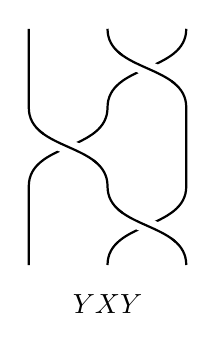
\begin{tikzpicture}
    \begin{knot}[clip width=7]
      \strand[thick] (0,0)
        to (0,-1)
        to [out=down,in=up] (1,-2)
        to [out=down,in=up] (2,-3);
      \strand[thick] (1,0)
        to [out=down,in=up] (2,-1)
        to (2,-2)
        to [out=down,in=up] (1,-3);
      \strand[thick] (2,0)
        to [out=down,in=up] (1,-1)
        to [out=down,in=up] (0,-2)
        to (0,-3);
    \end{knot}
    \node at (1,-3.5) {$YXY$};
  \end{tikzpicture}
\] So: the 3-strand braid group is \emph{isomorphic} to the fundamental
group of the complement of the trefoil! You may enjoy checking this
algebraically, using generators and relations, and then figuring out how
this algebraic proof relates to the geometrical proof.

I find all this stuff very pretty\ldots{}

\ldots{} but what's really \emph{magnificent} is that most of it
generalizes to any Dynkin diagram, or even any Coxeter diagram! (See
\protect\hyperlink{week62}{``Week 62''} for those.)

Yes, we've secretly been studying the Coxeter diagram \(\mathrm{A}_2\),
whose ``Coxeter group'' is the group of permutations of 3 things, and
whose ``Weyl chambers'' look like this: \[
  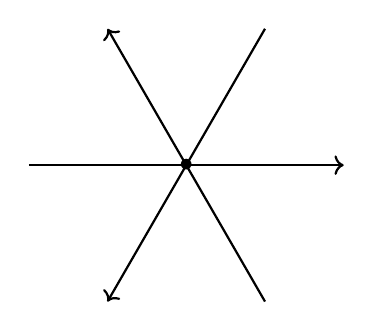
\begin{tikzpicture}
    \draw[thick,->] (180:2) to (0:2);
    \draw[thick,->] (-60:2) to (120:2);
    \draw[thick,->] (60:2) to (-120:2);
    \node at (0,0) {$\bullet$};
  \end{tikzpicture}
\] Let me just sketch how we can generalize this to
\(\mathrm{A}_{n-1}\). Here the Coxeter group is the group of
permutations of \(n\) things, which I'll call \(n!\).

Let \(X\) be the space of \(n\)-tuples of complex numbers summing to
\(0\). \(X\) is a complex vector space of dimension \(n-1\). We can
think of any point in \(X\) as the ordered \(n\)-tuple of roots of some
depressed polynomial of degree \(n\). Here ``depressed'' means that the
leading coefficient is \(1\) and the sum of the roots is zero. This
condition makes polynomials sad.

The permutation group \(n!\) acts on \(X\) in an obvious way. The
quotient \(X/n!\) is isomorphic (as a variety) to another complex vector
space of dimension \(n-1\): namely, the space of depressed polynomials
of degree \(n\). The quotient map \[X \to X/n!\] is just the map from
roots to coefficients!

Sitting inside \(X\) is the set \(D\) consisting of \(n\)-tuples of
roots where two or more roots are equal. \(D\) is the union of a bunch
of hyperplanes, as we saw in our example: \[
  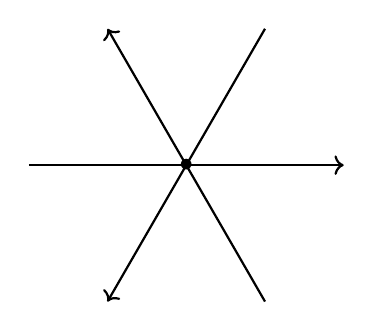
\begin{tikzpicture}
    \draw[thick,->] (180:2) to (0:2);
    \draw[thick,->] (-60:2) to (120:2);
    \draw[thick,->] (60:2) to (-120:2);
    \node at (0,0) {$\bullet$};
  \end{tikzpicture}
\] Sitting inside \(X/n!\) is the ``discriminant locus'' \(D/n!\),
consisting of \emph{degenerate} depressed polynomials of degree \(n\)
--- that is, those with two or more roots equal. This is a variety
that's smooth except for some sort of ``cusp'' at the origin: \[
  \begin{tikzpicture}
    \begin{axis}[
      axis x line=middle,
      axis y line=middle,
      ticks=none,
      xlabel={$B$},
      ylabel={$C$},
      xmin=-1,xmax=1
      ]
      \addplot[thick,domain=-1:1,samples=50] ({-x^2},{x^3});
    \end{axis}
  \end{tikzpicture}
\] The fundamental group of the complement of the discriminant locus is
the braid group on \(n\) strands. The reason is that this group
describes homotopy classes of ways that n points in the plane can move
around and come back to where they were (but possibly permuted). These
points are the roots of our polynomial.

On the other hand, the discriminant locus is topologically the cone on
some higher-dimensional knot sitting inside the unit sphere in
\(\mathbb{C}^{n-1}\). So, the fundamental group of the complement of
this knot is the braid group on \(n\) strands.

This relation between higher-dimensional knots and singularities was
investigated by Milnor, not just for the \(\mathrm{A}_n\) series of
Coxeter diagrams but more generally:

\begin{enumerate}
\def\labelenumi{\arabic{enumi})}
\setcounter{enumi}{6}
\tightlist
\item
  John W. Milnor, \emph{Singular Points of Complex Hypersurfaces},
  Princeton U. Press, 1969.
\end{enumerate}

The other Coxeter diagrams give generalizations of braid groups called
Artin-Brieskorn groups. Algebraically you get them by taking the usual
presentations of the Coxeter groups and dropping the relations saying
the generators (reflections) square to \(1\).

If you like braid groups and Dynkin diagrams, Artin-Brieskorn groups are
irresistible! For a fun modern account, try:

\begin{enumerate}
\def\labelenumi{\arabic{enumi})}
\setcounter{enumi}{7}
\tightlist
\item
  Daniel Allcock, ``Braid pictures for Artin groups'', available as
  \href{http://arxiv.org/abs/math.GT/9907194}{\texttt{arXiv:math.GT/9907194}}.
\end{enumerate}

But I'm digressing! I must return and finish my ode to the number 3. I
need to say how modular forms get into the game!

I'll pick up the pace a bit now --- if you're tired, quit here.

Any cubic polynomial \(P(x)\) gives something called an ``elliptic
curve''. This consists of all the complex solutions of \[y^2 = P(x)\]
together with the point \((\infty, \infty)\), which we include to make
things nicer.

Clearly this elliptic curve has two points \((x,y)\) for each value of
\(x\) \emph{except} for \(x = \infty\) and the roots of \(P(x)\), where
it just has one. So, it's a ``branched double cover'' of the Riemann
sphere, with branch points at the roots of our cubic and the point at
infinity.

In fact, this elliptic curve has the topology of a torus, at least when
all the roots of our cubic are different. If you have trouble imagining
a torus that's a branched double cover of a sphere, ponder this:
\[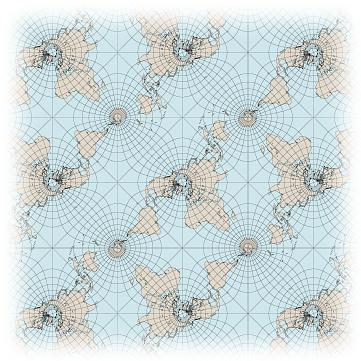
\includegraphics[max width=0.65\linewidth]{../images/quincuncial_tiled.jpg}\]

\begin{enumerate}
\def\labelenumi{\arabic{enumi})}
\setcounter{enumi}{8}
\tightlist
\item
  Carlos Furuti, ``Peirce's quincuncial map'',
  \texttt{http://www.progonos.com/furuti/MapProj/Normal/ProjConf/projConf.html}
\end{enumerate}

This square map of the Earth is an unwrapped torus; each point of the
Earth shows up lots of times. If we wrap it up just right, we get a
branched double cover of the sphere! Can you spot the branch points? For
a lot more explanation, read \protect\hyperlink{week229}{``Week 229''}.

Now, way back in \protect\hyperlink{week13}{``Week 13''}, I turned this
story around. I started with a torus formed as the quotient of the
complex plane by a lattice --- and showed how to get an elliptic curve
out of it. I wrote the equation for this elliptic curve in ``Weierstrass
form'': \[y^2 = 4x^3 - g_2 x - g_3\] By a simple change of variables,
this is equivalent to a depressed cubic: \[y^2 = x^3 + Bx + C\] So, we
can think of \(g_2\) and \(g_3\) as coordinates on our 2d space of
depressed cubics! They're just rescaled versions of our coordinate
functions \(B\) and \(C\).

What's the big deal? Well, \(g_2\) and \(g_3\) are famous examples of
``modular forms'' --- whatever those are. In fact, it's a famous fact
that every modular form is a polynomial in \(g_2\) and \(g_3\).

I defined modular forms back in \protect\hyperlink{week142}{``Week
142''}, where I summarized the Taniyama-Shimura-Weil theorem: the big
theorem about modular forms that implies Fermat's Last Theorem. So, you
can reread the definition there if you're curious. But if you've never
seen it before, it's a bit intimidating. A modular form of weight \(w\)
is a function on the space of lattices that transforms in a certain
bizarre way, satisfying a certain growth condition\ldots{} blah blah
blah.

It's important stuff, and incredibly cool once you get a feel for it.
But suppose we're trying to explain modular forms more simply. Then we
can avoid a lot of technicalities if we just say a modular form is a
polynomial on the space of depressed cubics! In other words, a
polynomial in our friends \(B\) and \(C\).

Then we can make some definitions. The ``weight'' of the modular form
\[B^i C^j\] is \(4i+6j\). Okay, I admit this sounds arbitrary and weird
without a lot more explanation. But better: a ``cusp form'' is a modular
form that vanishes on the discriminant locus. Then we can see every cusp
form is the product of the discriminant \(4B^3 + 27C^2\) and some other
modular form\ldots{} and we can use this to work out lots of basic stuff
about modular forms.

So, I hope you now see how tightly entwined all these ideas are:

\begin{itemize}
\tightlist
\item
  the trefoil knot
\item
  cubic polynomials
\item
  the group of permutations of 3 things
\item
  the three-strand braid group
\item
  modular forms and cusp forms
\end{itemize}

At this point I should give credit where credit is due. As usual, I've
been talking to Jim Dolan, and many of these ideas come from him. But
also, you can think of this Week as an expansion of the remarks by Joe
Christy and Swiatowslaw Gal in the Addenda to
\protect\hyperlink{week233}{``Week 233''}. And, it was Chris Hillman who
first told Jim and me that
\(\mathrm{SL}(2,\mathbb{R})/\mathrm{SL}(2,\mathbb{Z})\) looks like
\(S^3\) minus a trefoil knot.

Finally, I should say that my low-budget approach to modular forms
mostly just handles so-called ``level \(0\)'' modular forms --- the
basic kind, defined using the group
\[\Gamma = \mathrm{PSL}(2,\mathbb{Z})\] More exciting are modular forms
that transform nicely only for a \emph{subgroup} of \(\Gamma\). Jim and
I are just beginning to understand these. But the modular forms for
\(\Gamma(2)\) fit nicely into today's ode! Here \(\Gamma(2)\) is the
subgroup of \(\Gamma\) consisting of matrices congruent to the identity
matrix \(\mod 2\). What does this have to do with my ode to the number
3? Well, \[\Gamma/\Gamma(2) \cong \mathrm{PSL}(2,\mathbb{F}_2)\] and
this is isomorphic to the group of permutations of 3 things!

So, as a final flourish, I claim that:

Modular forms for \(\Gamma(2)\) are polynomials on the space \(X\)
consisting of roots of depressed cubics:
\[X = \{(a,b,c) \mid \mbox{$a,b,c$ complex with $a + b + c = 0$}\}\]
Modular forms for \(\Gamma\) are polynomials on the space \(X/3!\)
consisting of coefficients of depressed cubics:
\[X/3! = \{(B,C) \mid \mbox{$B,C$ complex}\}\] The obvious quotient map
\(X \to X/3!\) sends roots to coefficients:
\[(a,b,c) \mapsto (B,C) = (ab + bc + ca, abc)\] and this induces the
inclusion of modular forms for \(\Gamma\) into modular forms for
\(\Gamma(2)\): \[
  \begin{aligned}
    B &\mapsto ab + bc + ca
  \\C &\mapsto abc
  \end{aligned}
\] I hope this is all true!

Modular forms for \(\Gamma(2)\) are particularly nice. A good example is
the \emph{cross-ratio}, much beloved in complex analysis. If you want to
learn more about this stuff, try:

\begin{enumerate}
\def\labelenumi{\arabic{enumi})}
\setcounter{enumi}{9}
\tightlist
\item
  Igor V. Dolgachev, ``Lectures on modular forms'', Fall 1997/8,
  available at
  \texttt{http://www.math.lsa.umich.edu/\textasciitilde{}idolga/modular.pdf}
\end{enumerate}

especially chapter 9 for level 2 modular forms. Also:

\begin{enumerate}
\def\labelenumi{\arabic{enumi})}
\setcounter{enumi}{10}
\tightlist
\item
  Henry McKean and Victor Moll, \emph{Elliptic Curves: Function Theory,
  Geometry, Arithmetic}, Cambridge U. Press, 1999.
\end{enumerate}

especially chapter 4.

\begin{center}\rule{0.5\linewidth}{0.5pt}\end{center}

\textbf{Addendum:} For more discussion, go to the
\href{http://golem.ph.utexas.edu/category/2007/12/this_weeks_finds_in_mathematic_20.html}{\(n\)-Category
Café}.

\begin{center}\rule{0.5\linewidth}{0.5pt}\end{center}

\begin{quote}
\emph{It is difficult to give an idea of the vast extent of modern
mathematics. The word ``extent'' is not the right one: I mean extent
crowded with beautiful detail --- not an extent of mere uniformity such
as an objectless plain, but a tract of beautiful country to be rambled
through and studied to every detail of hillside and valley, stream,
rock, wood and flower.}

--- Arthur Cayley
\end{quote}



\hypertarget{week262}{%
\section{March 29, 2008}\label{week262}}

I'm done with teaching until fall, and now I'll be travelling a lot. I
just got back from Singapore. It's an incredibly diverse place. I
actually had to buy a book to understand all the foods! I'm now
acquainted with the charms of
\href{http://en.wikipedia.org/wiki/Appam}{appam},
\href{http://en.wikipedia.org/wiki/Kaya_toast}{kaya toast}, and
\href{http://pachome1.pacific.net.sg/~ccchia/recipe03.html}{babi buah
keluak}. But I didn't get around to trying a
\href{http://en.wikipedia.org/wiki/Cendol}{chendol}, a
\href{http://en.wikipedia.org/wiki/Bandung_\%28drink\%29}{bandung}, or a
\href{http://en.wikipedia.org/wiki/Milo_\%28drink\%29\#Use}{Milo
dinosaur}, even though they're all available in every
\href{http://en.wikipedia.org/wiki/Hawker_centre}{hawker center}.

Today I'll talk about quantum technology in Singapore, atom chips,
graphene transistors, nitrogen-vacancy pairs in diamonds, a new
construction of \(\mathfrak{e}_8\), and a categorification of quantum
\(\mathfrak{sl}(2)\).

But first --- the astronomy pictures of the week!

First another planetary nebula --- the ``Southern Ring Nebula'':
\[\href{http://heritage.stsci.edu/1998/39/big.html}{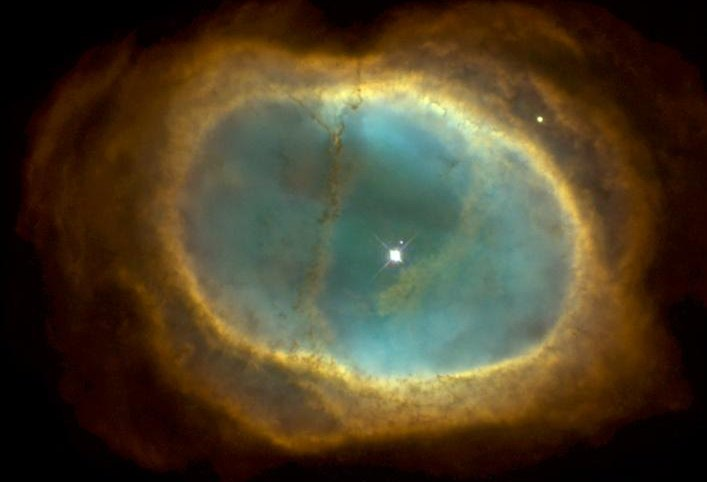
\includegraphics[max width=0.65\linewidth]{../images/NGC3132.jpg}}\]

\begin{enumerate}
\def\labelenumi{\arabic{enumi})}
\tightlist
\item
  Hubble Heritage Project, ``Planetary Nebula NGC 3132'',
  \texttt{http://heritage.stsci.edu/1998/39/index.html}
\end{enumerate}

This bubble of hot gas is .4 light years in diameter. You can see
\emph{two} stars near its center. The faint one is the white dwarf
remnant of the star that actually threw off the gas forming this nebula.
The gas is expanding outwards at about 20 kilometers per second. The
intense ultraviolet radiation from the white dwarf is ionizing this gas
and making it glow.

The Southern Ring Nebula is 2000 light years from us. Much closer to
home, here's a new shot of the frosty dunes of Mars:
\[\href{http://hirise-pds.lpl.arizona.edu/PDS/EXTRAS/RDR/PSP/ORB_007000_007099/PSP_007043_2650/PSP_007043_2650_RGB.NOMAP.browse.jpg}{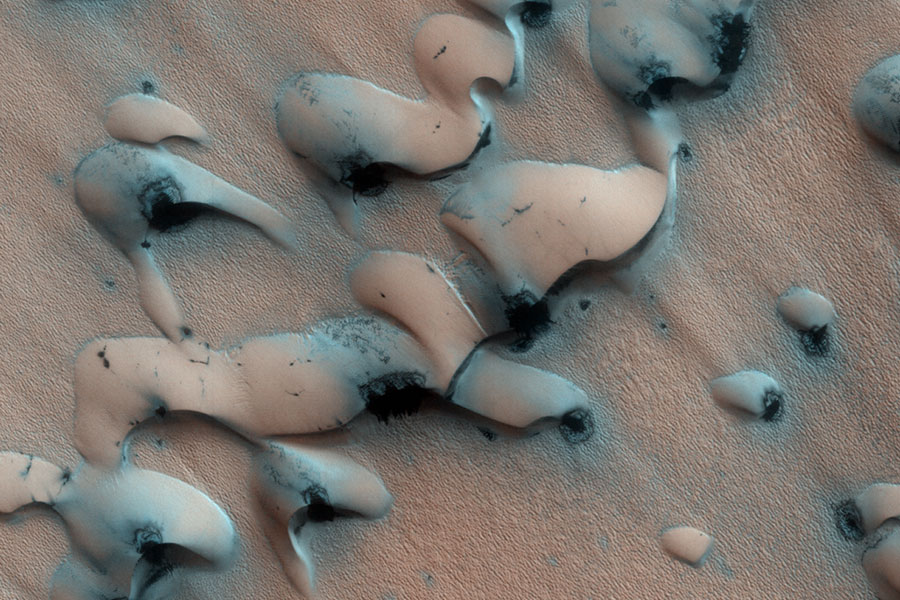
\includegraphics[max width=0.65\linewidth]{../images/mars_barchans_1.jpg}}\]

\begin{enumerate}
\def\labelenumi{\arabic{enumi})}
\setcounter{enumi}{1}
\tightlist
\item
  HiRISE (High Resolution Imaging Science Experiment), ``Defrosting
  polar sand dunes'',
  \texttt{http://hirise.lpl.arizona.edu/PSP\_007043\_2650}
\end{enumerate}

These horn-shaped dunes are called ``barchans''; you can read more about
them at \protect\hyperlink{week228}{``Week 228''}. The frost is carbon
dioxide, evaporating as the springtime sun warms the north polar region.
Here's another photo, taken in February:
\[\href{http://hirise-pds.lpl.arizona.edu/PDS/EXTRAS/RDR/PSP/ORB_007100_007199/PSP_007193_2640/PSP_007193_2640_RGB.NOMAP.browse.jpg}{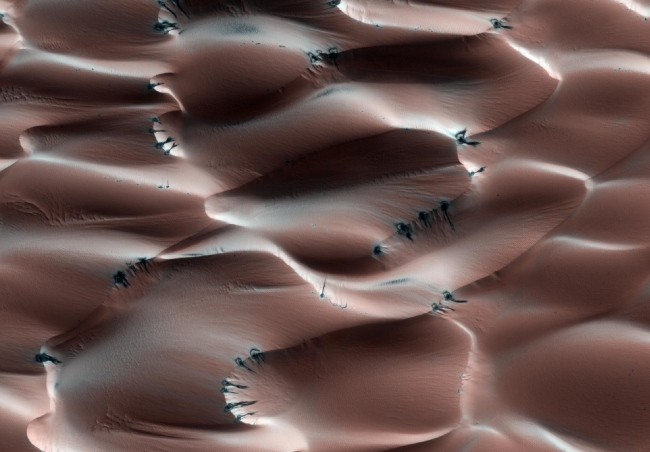
\includegraphics[max width=0.65\linewidth]{../images/mars_barchans_2.jpg}}\]

\begin{enumerate}
\def\labelenumi{\arabic{enumi})}
\setcounter{enumi}{2}
\tightlist
\item
  HiRISE (High Resolution Imaging Science Experiment), ``Defrosting
  northern dunes'',
  \texttt{http://hirise.lpl.arizona.edu/PSP\_007193\_2640}
\end{enumerate}

The dark stuff pouring down the steep slopes reminds me of water, but
they say it's dust!

(If you click on these Mars photos, you'll get some amazing larger
views.)

Meanwhile, down here on Earth, I had some good conversations with
mathematicians and physicists at the National University of Singapore
(NUS), and also with Artur Ekert and Valerio Scarani, who work here:

\begin{enumerate}
\def\labelenumi{\arabic{enumi})}
\setcounter{enumi}{3}
\tightlist
\item
  Centre for Quantum Technologies, \texttt{http://www.quantumlah.org/}
\end{enumerate}

I like the name ``quantumlah''. ``Lah'' is perhaps the most famous word
in Singlish: you put it at the end of a sentence for emphasis, to convey
``acceptance, understanding, lightness, jest, and a medley of other
positive feelings''. Unfortunately I didn't get to hear much Singlish
during my visit.

The Centre for Quantum Technologies is hosted by NUS but is somewhat
independent. It reminds me a bit of the Institute for Quantum Computing
--- see \protect\hyperlink{week235}{``Week 235''} --- but it's smaller,
and still getting started. They hope to take advantage of the nearby
semiconductor fabrication plants, or ``fabs'', to build stuff.

They've got theorists and experimentalists. Being overly theoretical
myself, I asked: what are the most interesting real-life working devices
we're likely to see soon? Ekert mentioned ``quantum repeaters'' ---
gadgets that boost the power of a beam of entangled photons while still
maintaining quantum coherence, as needed for long-distance quantum
cryptography. He also mentioned ``atom chips'', which use tiny wires
embedded in a silicon chip to trap and manipulate cold atoms on the
chip's surface:

\begin{enumerate}
\def\labelenumi{\arabic{enumi})}
\setcounter{enumi}{4}
\item
  Atomchip Group, \texttt{http://www.atomchip.org/}
\item
  Atom Optics Group, Laboratoire Charles Fabry, ``Atom-chip
  experiment'',
  \texttt{http://atomoptic.iota.u-psud.fr/research/chip/chip.html}
\end{enumerate}

There's also a nanotech group at NUS:

\begin{enumerate}
\def\labelenumi{\arabic{enumi})}
\setcounter{enumi}{6}
\tightlist
\item
  Nanoscience and Nanotechnology Initiative, National University of
  Singapore, \texttt{http://www.nusnni.nus.edu.sg/}
\end{enumerate}

who are doing cool stuff with ``graphene'' --- hexagonal sheets of
carbon atoms, like individual layers of a graphite crystal:
\[\href{http://en.wikipedia.org/wiki/Graphene}{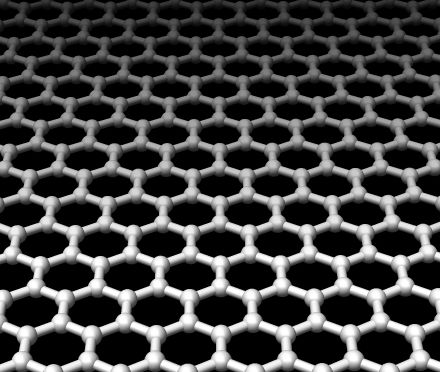
\includegraphics[max width=0.65\linewidth]{../images/graphene.jpg}}\]
Graphene is closely related to buckyballs (see
\protect\hyperlink{week79}{``Week 79''}) and polycyclic aromatic
hydrocarbons (see \protect\hyperlink{week258}{``Week 258''}).

Some researchers believe that graphene transistors could operate in the
terahertz range, about 1000 times faster than conventional silicon ones.
The reason is that electrons move much faster through graphene.
Unfortunately the difference in conductivity between the ``on'' and
``off'' states is less for graphene. This makes it harder to work with.
People think they can solve this problem, though:

\begin{enumerate}
\def\labelenumi{\arabic{enumi})}
\setcounter{enumi}{7}
\item
  Kevin Bullis, ``Graphene transistors'', \emph{Technology Review},
  January 28, 2008,
  \texttt{http://www.technologyreview.com/Nanotech/20119/}

  Duncan Graham-Rowe, ``Better graphene transistors'', \emph{Technology
  Review}, March 17, 2008,
  \texttt{http://www.technologyreview.com/Nanotech/20424/}
\end{enumerate}

Ekert also told me about another idea for carbon-based computers:
``nitrogen-vacancy centers''. These are very elegant entities. To
understand them, it helps to know a bit about diamonds. You really just
need to know that diamonds are crystals made of carbon. But I can't
resist saying more, because the geometry of these crystals is
fascinating.

A diamond is made of carbon atoms arranged in tetrahedra, which then
form a cubical structure, like this:
\[\href{http://newton.ex.ac.uk/research/qsystems/people/sque/diamond/structure/}{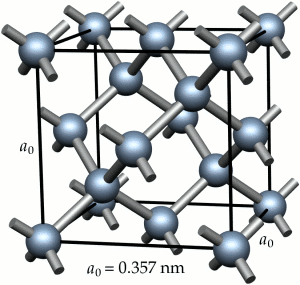
\includegraphics[max width=0.65\linewidth]{../images/diamond-conventional-unit-cell.png}}\]

\begin{enumerate}
\def\labelenumi{\arabic{enumi})}
\setcounter{enumi}{8}
\tightlist
\item
  Steve Sque, ``Structure of diamond'',
  \texttt{http://newton.ex.ac.uk/research/qsystems/people/sque/diamond/structure/}
\end{enumerate}

Here you see 4 tetrahedra of carbon atoms inside a cube. Note that
there's one carbon at each corner of the cube, and also one in the
middle of each face. If that was all, we'd have a ``face-centered
cubic''. But there are also 4 more carbons inside the cube --- one at
the center of each tetrahedron!

If you look really carefully, you can see that the full pattern consists
of two interpenetrating face-centered cubic lattices, one offset
relative to the other along the cube's main diagonal!

While the math of the diamond crystal is perfectly beautiful, nature
doesn't always get it quite right. Sometimes a carbon atom will be
missing. In fact, sometimes a cosmic ray will knock a carbon out of the
lattice! You can also do it yourself with a beam of neutrons or
electrons. The resulting hole is called a ``vacancy''. If you heat a
diamond to about 900 kelvin, these vacancies start to move around like
particles.

Diamonds also have impurities. The most common is nitrogen, which can
form up 1\% of a diamond. Nitrogen atoms can take the place of carbon
atoms in the crystal. Sometimes these nitrogen atoms are isolated,
sometimes they come in pairs.

When a lone nitrogen encounters a vacancy, they stick together! We then
have a ``nitrogen-vacancy center''. It's also common for 4 nitrogens to
surround a vacancy. Many other combinations are also possible --- and
when we get enough of these nitrogen-vacancy combinations around, they
form larger structures called ``platelets''.

\begin{enumerate}
\def\labelenumi{\arabic{enumi})}
\setcounter{enumi}{9}
\tightlist
\item
  R. Jones and J. P. Goss, ``Theory of aggregation of nitrogen in
  diamond'', in \emph{Properties, Growth and Application of Diamond},
  eds.~Maria Helena Nazare and A. J. Neves, EMIS Datareviews Series,
  2001, 127--130.
\end{enumerate}

A nice thing about nitrogen-vacancy centers is that they act like
spin-\(1\) particles. In fact, these spins interact very little with
their environment, thanks to the remarkable properties of diamond. So,
they might be a good way to store quantum information: they can last 50
microseconds before losing coherence, even at room temperature. If we
could couple them to each other in interesting ways, maybe we could do
some ``spintronics'', or even quantum computation:

\begin{enumerate}
\def\labelenumi{\arabic{enumi})}
\setcounter{enumi}{10}
\tightlist
\item
  Sankar das Sarma, ``Spintronics'', \emph{American Scientist}
  \textbf{89} (2001), 516--523. Also available at
  \texttt{http://www.physics.umd.edu/cmtc/earlier\_papers/AmSci.pdf}
\end{enumerate}

Lone nitrogens are even more robust carriers of quantum information:
their time to decoherence can be as much as a millisecond! The reason is
that, unlike nitrogen-vacancy centers, lone nitrogens have ``dark
spins'' --- their spin doesn't interact much with light. But this can
also makes them harder to manipulate. So, it may be easier to use
nitrogen-vacancy centers. People are busy studying the options:

\begin{enumerate}
\def\labelenumi{\arabic{enumi})}
\setcounter{enumi}{11}
\item
  R. J. Epstein, F. M. Mendoza, Y. K. Kato and D. D. Awschalom,
  ``Anisotropic interactions of a single spin and dark-spin spectroscopy
  in diamond'', \emph{Nature Physics} \textbf{1} (2005), 94--98. Also
  available as
  \href{http://arxiv.org/abs/cond-mat/0507706}{\texttt{arXiv:cond-mat/0507706}}.
\item
  Ph. Tamarat et al, ``The excited state structure of the
  nitrogen-vacancy center in diamond'', available as
  \href{http://arxiv.org/abs/cond-mat/0610357}{\texttt{arXiv:cond-mat/0610357}}.
\item
  R. Hanson, O. Gywat and D. D. Awschalom, ``Room-temperature
  manipulation and decoherence of a single spin in diamond'',
  \emph{Phys. Rev.} \textbf{B74} (2006) 161203. Also available as
  \href{http://arxiv.org/abs/quant-ph/0608233}{\texttt{quant-ph/0608233}}
\end{enumerate}

But regardless of whether anyone can coax them into quantum computation,
I like diamonds. Not to own --- just to contemplate! I told you about
the diamond rain on Neptune back in \protect\hyperlink{week160}{``Week
160''}. And in \protect\hyperlink{week193}{``Week 193''}, I explained
how diamonds are the closest thing to the \(\mathrm{E}_8\) lattice
you're likely to see in this \(3\)-dimensional world.

The reason is that in any dimension you can define a checkerboard
lattice called \(\mathrm{D}_n\), consisting of all \(n\)-tuples of
integers that sum to an even integer. Then you can define a set called
\(\mathrm{D}_n^+\) by taking two copies of the \(\mathrm{D}_n\) lattice:
the original and another shifted by the vector \((1/2,\ldots,1/2)\).
\(\mathrm{D}_8^+\) is the \(\mathrm{E}_8\) lattice, but \(\mathrm{D}_3\)
is the face-centered cubic, and \(\mathrm{D}_3^+\) is the pattern formed
by carbons in a diamond!

In case you're wondering: in math, unlike crystallography, we reserve
the term ``lattice'' for a discrete subgroup of \(\mathbb{R}^n\) that's
isomorphic to \(\mathbb{Z}^n\). The set \(\mathrm{D}_n^+\) is only
closed under addition when \(n\) is even. So, the carbons in a diamond
don't form a lattice in the strict mathematical sense. On the other
hand, the face-centered cubic really is a lattice, the \(\mathrm{D}_3\)
lattice --- and this is secretly the same as the \(\mathrm{A}_3\)
lattice, familiar from stacking oranges. It's one of the densest ways to
pack spheres, with a density of \[\frac{\pi}{3\sqrt2} \approx 0.74.\]
The \(\mathrm{D}_3^+\) pattern, on the other hand, has a density of just
\[\frac{\pi\sqrt3}{16} \approx 0.34.\] This is why ice becomes denser
when it melts: it's packed in a close relative of the \(\mathrm{D}_3^+\)
pattern, with an equally low density.

(Do diamonds become denser when they melt? Or do they always turn into
graphite when they get hot enough, regardless of the pressure? Inquiring
minds want to know. These days inquiring minds use search engines to
answer questions like this\ldots{} but right now I'd rather talk about
\(\mathrm{E}_8\).)

As you probably noticed, Garrett Lisi stirred up quite a media sensation
with his attempt to pack all known forces and particles into a theory
based on the exceptional Lie group \(\mathrm{E}_8\):

\begin{enumerate}
\def\labelenumi{\arabic{enumi})}
\setcounter{enumi}{14}
\tightlist
\item
  Garrett Lisi, ``An exceptionally simple theory of everything'',
  available as
  \href{http://arxiv.org/abs/0711.0770}{\texttt{arXiv:0711.0770}}
\end{enumerate}

Part of his idea was to use Kostant's triality-based description of
\(\mathrm{E}_8\) to explain the three generations of leptons --- see
\protect\hyperlink{week253}{``Week 253''} for more. Unfortunately this
part of the idea doesn't work, for purely group-theoretical reasons:

\begin{enumerate}
\def\labelenumi{\arabic{enumi})}
\setcounter{enumi}{15}
\tightlist
\item
  Jacques Distler, ``A little group theory'',
  \texttt{http://golem.ph.utexas.edu/\textasciitilde{}distler/blog/archives/001505.html},
  ``A little more group theory'',
  \texttt{http://golem.ph.utexas.edu/\textasciitilde{}distler/blog/archives/001532.html}
\end{enumerate}

There would also be vast problems trying get all the dimensionless
constants in the Standard Model to pop out of such a scheme --- or to
stick them in somehow.

Meanwhile, Kostant has been doing new things with \(\mathrm{E}_8\). He's
mainly been using the complex form of \(\mathrm{E}_8\), while Lisi needs
a noncompact real form to get gravity into the game. So, the connection
between their work is somewhat limited. Nonetheless, Kostant enjoys the
idea of a theory of everything based on \(\mathrm{E}_8\).

He recently gave a talk here at UCR:

\begin{enumerate}
\def\labelenumi{\arabic{enumi})}
\setcounter{enumi}{16}
\tightlist
\item
  Bertram Kostant, `On some mathematics in Garrett Lisi's
  ``\(\mathrm{E}_8\) theory of everything''\,', February 12, 2008, UCR.
  Video and lecture notes at
  \texttt{http://math.ucr.edu/home/baez/kostant/}
\end{enumerate}

He did some amazing things, like chop the \(248\)-dimensional Lie
algebra of \(\mathrm{E}_8\) into 31 Cartan subalgebras in a nice way,
thus categorifying the factorization \[248 = 8 \times 31\] To do this,
he used a copy of the \(32\)-element group \((\mathbb{Z}/2)^5\) sitting
in \(\mathrm{E}_8\), and the 31 nontrivial characters of this group.

Even more remarkably, this copy of \((\mathbb{Z}/2)^5\) sits inside a
copy of \(\mathrm{SL}(2,\mathbb{F}_{32})\) inside \(\mathrm{E}_8\), and
the centralizer of a certain element of
\(\mathrm{SL}(2,\mathbb{F}_{32})\) is a product of two copies of the
gauge group of the Standard Model! What this means --- if anything ---
remains a mystery.

Indeed, pretty much everything about \(\mathrm{E}_8\) seems mysterious
to me, since nobody has exhibited it as the symmetry group of anything
more comprehensible than \(\mathrm{E}_8\) itself. This paper sheds some
new light this puzzle:

\begin{enumerate}
\def\labelenumi{\arabic{enumi})}
\setcounter{enumi}{16}
\tightlist
\item
  José Miguel Figueroa-O'Farrill, ``A geometric construction of the
  exceptional Lie algebras \(\mathrm{F}_4\) and \(\mathrm{E}_8\)'',
  available as
  \href{http://arxiv.org/abs/0706.2829}{\texttt{arXiv:0706.2829}}.
\end{enumerate}

The idea here is to build the Lie algebra of \(\mathrm{E}_8\) using
Killing spinors on the unit sphere in 16 dimensions.

Okay --- what's a Killing spinor?

Well, first I need to remind you about Killing vectors. Given a
Riemannian manifold, a ``Killing vector'' is a vector field that
generates a flow that preserves the metric! A transformation that
preserves the metric is called an ``isometry'', and these form a Lie
group. Killing vector fields form a Lie algebra if we use the ordinary
Lie bracket of vector fields, and this is the Lie algebra of the group
of isometries.

Now, if our manifold has a spin structure, a ``Killing spinor'' is a
spinor field \(\psi\) such that \[D_v\psi = k v\psi\] for some constant
\(k\) for every vector field \(v\). Here \(D_v\psi\) is the covariant
derivative of \(\psi\) in the \(v\) direction, while \(v\psi\) is
defined using the action of vectors on spinors. Only the sign of the
constant k really matters, since rescaling the metric rescales this
constant.

It's a cute equation, but what's the point of it? Part of the point is
this: the action of vectors on spinors \[V \otimes S \to S\] has a kind
of adjoint \[S \otimes S \to V\] This lets us take a pair of spinor
fields and form a vector field. This is what people mean when they say
spinors are like the ``square root'' of vectors. And, if we do this to
two \emph{Killing} spinors, we get a \emph{Killing} vector! You can
prove this using that cute equation --- and that's the main point of
that equation, as far as I'm concerned.

Under good conditions, this fact lets us define a ``Killing
superalgebra'' which has the Lie algebra of Killing vectors as its even
part, and the Killing spinors as its odd part.

In this superalgebra, the bracket of two Killing vectors is just their
ordinary Lie bracket. The bracket of a Killing vector and a Killing
spinor is defined using a fairly obvious notion of the ``Lie derivative
of a spinor field''. And, the bracket of two Killing spinors is defined
using the map \[S \otimes S \to V\] which, as explained, gives a Killing
vector.

Now, you might think our ``Killing superalgebra'' should be a Lie
superalgebra. But in some dimensions, the map \[S \otimes S \to V\] is
skew-symmetric. Then our Killing superalgebra has a chance at being a
plain old Lie algebra! We still need to check the Jacobi identity. And
this only works in certain special cases:

If you take \(S^7\) with its usual round metric, the isometry group is
\(\mathrm{SO}(8)\), so the Lie algebra of Killing vectors is
\(\mathfrak{so}(8)\). There's an 8-dimensional space of Killing spinors,
and the action of \(\mathfrak{so}(8)\) on this gives the real
left-handed spinor representation \(S_8^+\). The Jacobi identity holds,
and you get a Lie algebra structure on \[\mathfrak{so}(8) \oplus S_8^+\]
But then, thanks to triality, you knock yourself on the head and say ``I
could have had a \(V_8\)!'' After all, up to an outer automorphism of
\(\mathfrak{so}(8)\), the spinor representation \(S_8^+\) is the same as
the \(8\)-dimensional vector representation \(V_8\). So, your Lie
algebra is the same as \[\mathfrak{so}(8) \oplus V_8\] with a certain
obvious Lie algebra structure. This is just \(\mathfrak{so}(9)\). So,
it's nothing exceptional, though you arrived at it by a devious route.

If you take \(S^8\) with its usual round metric, the Lie algebra of
Killing vector fields is \(\mathfrak{so}(9)\). Now there's a
\(16\)-dimensional space of Killing spinor fields, and the action of
\(\mathfrak{so}(9)\) on this gives the real (non-chiral) spinor
representation \(S_9\). The Jacobi identity holds, and you get a Lie
algebra structure on \[\mathfrak{so}(9) \oplus S_9\] This gives the
exceptional Lie algebra \(\mathfrak{f}_4\)!

Finally, if you take \(S^{15}\) with its usual round metric, the Lie
algebra of Killing vector fields is \(\mathfrak{so}(16)\). Now there's a
\(128\)-dimensional space of Killing spinor fields, and the action of
\(\mathfrak{so}(16)\) on this gives the left-handed real spinor
representation \(S_{16}^+\). The Jacobi identity holds, and you get a
Lie algebra structure on \[\mathfrak{so}(16) \oplus S_{16}^+\] This
gives the exceptional Lie algebra \(\mathfrak{e}_8\)!

In short, what Figueroa-O'Farrill has done is found a nice geometrical
interpretation for some previously known algebraic constructions of
\(\mathfrak{f}_4\) and \(\mathfrak{e}_8\). Unfortunately, he still needs
to verify the Jacobi identity in the same brute-force way. It would be
nice to find a slicker proof. But his new interpretation is suggestive:
it raises a lot of new questions. He lists some of these at the end of
the paper, and mentions a really big one at the beginning. Namely: the
spheres \(S^7\), \(S^8\) and \(S^{15}\) all show up in the Hopf
fibration associated to the octonionic projective line:
\[S^7 \to S^{15} \to S^8\] Does this give a nice relation between
\(\mathfrak{so}(9)\), \(\mathfrak{f}_4\) and \(\mathfrak{e}_8\)? Can
someone guess what this relation should be? Maybe \(\mathfrak{e}_8\) is
built from \(\mathfrak{so}(9)\) and \(\mathfrak{f}_4\) somehow.

I also wonder if there's a Killing superalgebra interpretation of the
Lie algebra constructions
\[\mathfrak{e}_6 = \mathfrak{so}(10) \oplus S_{10} \oplus \mathfrak{u}(1)\]
and
\[\mathfrak{e}_7 = \mathfrak{so}(12) \oplus S_{12}^+ \oplus \mathfrak{su}(2)\]
These would need to be trickier, with the \(\mathfrak{u}(1)\) showing up
from the fact that \(S_{10}\) is a complex representation, and the
\(\mathfrak{su}(2)\) showing up from the fact that \(S_{12}^+\) is a
quaternionic representation. The algebra is explained here:

\begin{enumerate}
\def\labelenumi{\arabic{enumi})}
\setcounter{enumi}{17}
\tightlist
\item
  John Baez, \emph{The octonions}, section 4.3: ``the magic square'',
  available at
  \texttt{http://math.ucr.edu/home/baez/octonions/node16.html}
\end{enumerate}

A geometrical interepretation would be nice!

Finally --- my former student Aaron Lauda has been working with Khovanov
on categorifying quantum groups, and their work is starting to really
take off. I'm just beginning to read his new papers, but I can't resist
bringing them to your attention:

\begin{enumerate}
\def\labelenumi{\arabic{enumi})}
\setcounter{enumi}{18}
\item
  Aaron Lauda, ``A categorification of quantum \(\mathfrak{sl}(2)\)'',
  available as
  \href{http://arxiv.org/abs/0803.3652}{\texttt{arXiv:0803.3652}}.

  Aaron Lauda, ``Categorified quantum \(\mathfrak{sl}(2)\) and
  equivariant cohomology of iterated flag varieties'', available as
  \href{http://arxiv.org/abs/0803.3848}{\texttt{arXiv:0803.3848}}.
\end{enumerate}

He's got a \emph{\(2\)-category} that decategorifies to give the
quantized universal enveloping algebra of \(\mathfrak{sl}(2)\)! And
similarly for all the irreps of this algebra!

There's more to come, too\ldots.

\begin{center}\rule{0.5\linewidth}{0.5pt}\end{center}

\textbf{Addenda:} Starting this Week, you can see more discussion and
also \emph{questions I'm dying to know the answers to} over at the
\href{http://golem.ph.utexas.edu/category/2008/03/this_weeks_finds_in_mathematic_23.html}{\(n\)-Category
Café}. Whenever I write This Week's Finds, I come up with lots of
questions. If you can help me with some of these, I'll be really
grateful.

José Figueroa-O'Farrill sent an email saying:

\begin{quote}
About the geometric constructions of exceptional Lie algebras, you are
totally spot on in that what is missing is a more conceptual
understanding of the construction which would render the odd-odd-odd
component of the Jacobi identity `trivial', as is the case for the
remaining three components. One satisfactory way to achieve this would
be to understand of what in, say, the \(15\)-sphere is \(\mathrm{E}_8\)
the automorphisms. I'm afraid I don't have an answer.

As for \(\mathrm{E}_6\) and \(\mathrm{E}_7\), there is a similar
geometric construction for \(\mathrm{E}_6\) and one for \(\mathrm{E}_7\)
is in the works as part of a paper with Hannu Rajaniemi, who was a
student of mine. The construction is analogous, but for one thing. One
has to construct more than just the Killing vectors out of the Killing
spinors: in the case of \(\mathrm{E}_6\), it is enough to construct a
Killing \(0\)-form (i.e., a constant) which then acts on the Killing
spinors via a multiple of the Dirac operator. (This is consistent with
the action of `special Killing forms' a.k.a. `Killing-Yano tensors' on
spinors.) The odd-odd-odd Jacobi identity here is even more mysterious:
it does not simply follow from representation theory (i.e., absence of
invariants in the relevant representation where the `jacobator' lives),
but follows from an explicit calculation. The case of \(\mathrm{E}_7\)
should work in a similar way, but we still have not finished the
construction. (Hannu has a real job now and I've been busy with other
projects of a less `recreational' nature.) In

\begin{enumerate}
\def\labelenumi{\arabic{enumi})}
\setcounter{enumi}{19}
\tightlist
\item
  José Figueroa-O'Farrill, ``A geometrical construction of exceptional
  Lie algebras'', talk at Leeds, February 13, 2008, available at
  \texttt{http://www.maths.ed.ac.uk/\textasciitilde{}jmf/CV/Seminars/Leeds.pdf}
\end{enumerate}

you'll find the PDF version of a Keynote file I used for a geometry
seminar I gave recently on this topic in Leeds. This geometric
construction has its origin, as does the notion of Killing spinor
itself, in the early supergravity literature. Much of the early
literature on supergravity backgrounds was concerned with the so-called
Freund-Rubin backgrounds: product geometries \(L \times R\), with \(L\)
a lorentzian constant curvature spacetime and \(R\) a riemannian
homogeneous space and the only nonzero components of the flux were
proportional to the volume forms of \(L\) and/or \(R\). For such
backgrounds, supergravity Killing spinors, which are in bijective
correspondence with the supersymmetries of a (bosonic) background,
reduce to geometric Killing spinors.

To any supersymmetric supergravity background one can associate a Lie
superalgebra, called the Killing superalgebra. This is the superalgebra
generated by the Killing spinors; that is, if we let
\(K = K_0 \oplus K_1\) denote the Killing superalgebra, then
\[K_1 = \{\text{Killing spinors}\}\] and \[K_0 = [K_1,K_1]\] This is a
Lie superalgebra, due to the odd-odd Lie bracket being symmetric, as is
typical in lorentzian signature in the physically interesting
dimensions.

I gave a triangular seminar in London about this topic and you can find
slides here:

\begin{enumerate}
\def\labelenumi{\arabic{enumi})}
\setcounter{enumi}{20}
\tightlist
\item
  José Figueroa-O'Farrill, ``Killing superalgebras in supergravity'',
  talk at University of London, February 27, 2008, available at
  \texttt{http://www.maths.ed.ac.uk/\textasciitilde{}jmf/CV/Seminars/KSA.pdf}
\end{enumerate}

There is some overlap with the one in Leeds, but not too much.

Cheers, José
\end{quote}

These comments by Thomas Fischbacher should also fit into the big
picture somehow:

\begin{quote}
As you know, there is a nice triality symmetric construction of
\(\mathrm{E}_8\) that starts from
\(\mathrm{SO}(8)\times\mathrm{SO}(8)\). But, considering the maximally
split real form \(\mathrm{E}_8(8)\), did you also know that this
\(\mathrm{SO}(8)\times\mathrm{SO}(8)\) is best regarded as
\(\mathrm{SO}(8,\mathbb{C}^+)\), with \(\mathbb{C}^+\) being the
split-complex numbers with \(i^2=+1\)? There also are \(56\)-dimensional
real subgroups such as \(\mathrm{SO}(8,\mathbb{C})\) (2 different
embeddings --- ``IIA'' and ``IIB'') --- and there also is
\(\mathrm{SO}(8,\mathbb{C}0)\).

Basically, the way this works is that you can extend
\(\mathrm{SO}(8)\times\mathrm{SO}(8)\) to \$mathrm\{SO\}(16)\$ or
\(\mathrm{SO}(8,8)\) --- depending on whether you add the \(V\times V\)
or \(S\times S\) \(8\times8\)-block. But if you take diagonal
\(\mathrm{SO}(8)\) subgroups, then the \(8\times8\) all split into
\(28+35+1\), and you can play nice games with these 28's\ldots{}

See:

\begin{enumerate}
\def\labelenumi{\arabic{enumi})}
\setcounter{enumi}{21}
\tightlist
\item
  T. Fischbacher, H. Nicolai and H. Samtleben, ``Non-semisimple and
  complex gaugings of \(N = 16\) supergravity'', available as
  \href{http://arxiv.org/abs/hep-th/0306276\%22}{\texttt{hep-th/0306276}}.
\end{enumerate}
\end{quote}

\begin{center}\rule{0.5\linewidth}{0.5pt}\end{center}

\begin{quote}
\emph{A knowledge of the existence of something we cannot penetrate, of
the manifestations of the profoundest reason and the most radiant
beauty, which are only accessible to our reason in their most elementary
forms. It is this knowledge and this emotion that constitute the truly
religious attitude; in this sense, and in this alone, I am a deeply
religious man.}

--- Albert Einstein
\end{quote}



\hypertarget{week263}{%
\section{April 5, 2008}\label{week263}}

Enough nebulae! Today's astronomy picture is Saturn's moon Titan,
photographed by the Cassini probe. Red and green represent methane
absorption bands, while blue represents ultraviolet. Note the incredibly
deep atmosphere --- hundreds of kilometers deep. That's because Titan
has a dense atmosphere but not much gravity. The pale feature in the
center here is called Xanadu.
\[\href{http://apod.nasa.gov/apod/ap041028.html}{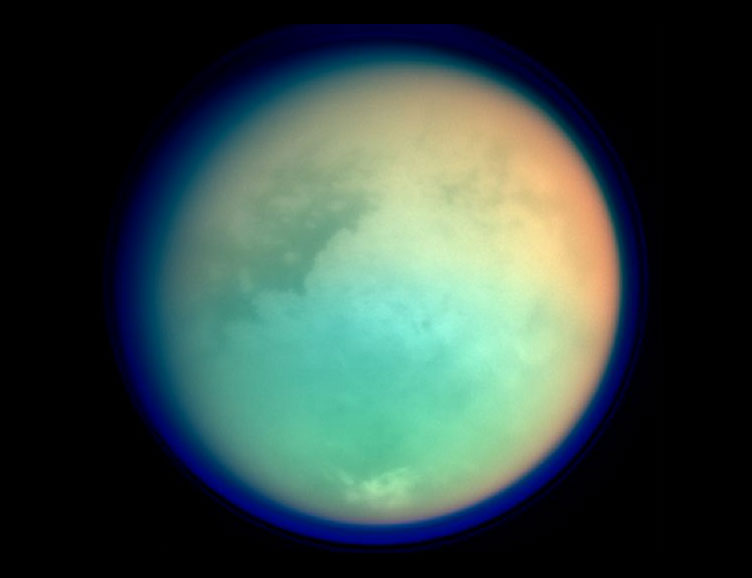
\includegraphics[max width=0.65\linewidth]{../images/titan.jpg}}\]

\begin{enumerate}
\def\labelenumi{\arabic{enumi})}
\tightlist
\item
  Astronomy Picture of the Day, ``Tantalizing Titan'',
  \texttt{http://apod.nasa.gov/apod/ap041028.html}
\end{enumerate}

If you fell into Titan's atmosphere, here's what you'd see. Unlike the
previous picture, this is in natural colors, taken by the Cassini probe
on March 31st, 2005 from a distance of just 9,500 kilometers:
\[\href{http://en.wikipedia.org/wiki/Titan_(moon)#Atmosphere}{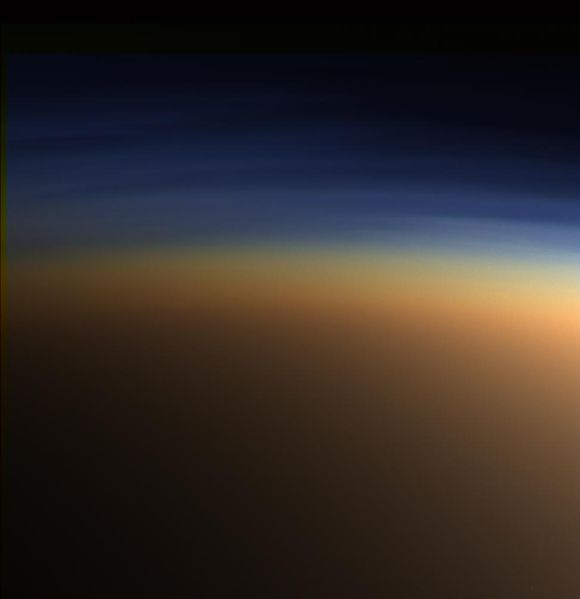
\includegraphics[max width=0.65\linewidth]{../images/titan_atmosphere.jpg}}\]

\begin{enumerate}
\def\labelenumi{\arabic{enumi})}
\setcounter{enumi}{1}
\tightlist
\item
  Wikipedia, ``Titan's atmosphere'',
  \texttt{http://en.wikipedia.org/wiki/Titan\_(moon)\#Atmosphere}
\end{enumerate}

The orange stuff is hydrocarbon ``smog'', perhaps made of chemicals
called \href{http://en.wikipedia.org/wiki/Tholin}{tholins} which I don't
really understand. When you got further down the atmosphere would be so
thick, and the gravity so low, that you could fly through it by flapping
wings attached to your arms. Unfortunately the atmosphere would be very
cold, and unbreathable: mostly nitrogen, with a little methane and
ethane. (I wrote about the hydrocarbon rain on Titan back in
\protect\hyperlink{week160}{``Week 160''}, and showed you the first
pictures of its lakes in \protect\hyperlink{week210}{``Week 210''}.)
\[\href{http://en.wikipedia.org/wiki/Titan_(moon)}{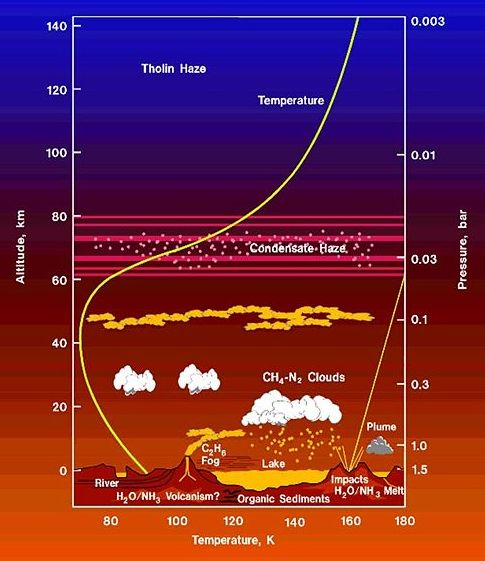
\includegraphics[max width=0.65\linewidth]{../images/titan_atmosphere_chart.jpg}}\]

Astronomy is great, but today I want to talk about group theory. As you
may have heard, John Thompson and Jacques Tits won the 2008 Abel prize
for their work on groups:

\begin{enumerate}
\def\labelenumi{\arabic{enumi})}
\setcounter{enumi}{2}
\tightlist
\item
  Abel Prize, ``2008 Laureates'',
  \texttt{http://www.abelprisen.no/en/prisvinnere/2008/}
\end{enumerate}

If you want a fun, nontechnical book that gives a good taste of the sort
of things Thompson thought about, try this:

\begin{enumerate}
\def\labelenumi{\arabic{enumi})}
\setcounter{enumi}{3}
\tightlist
\item
  Marcus du Sautoy, \emph{Symmetry: a Journey into the Patterns of
  Nature}, HarperCollins, 2008.
\end{enumerate}

Mathematicians will enjoy this book for its many anecdotes about the
heroes of symmetry, from Pythagoras to Thompson and other modern group
theorists. Nonmathematicians will learn a lot about group theory in a
fun easy way.

As a PhD student working under Saunders Mac Lane, Thompson began his
career with a bang, by solving a 60-year-old conjecture posed by the
famous group theorist Frobenius.

\begin{enumerate}
\def\labelenumi{\arabic{enumi})}
\setcounter{enumi}{4}
\tightlist
\item
  Mactutor History of Mathematics Archive, ``John Griggs Thompson'',
  \texttt{http://www-history.mcs.st-andrews.ac.uk/Biographies/Thompson\_John.html}
\end{enumerate}

But, he's mainly famous for helping prove an even harder theorem that's
even simpler to state --- one of those precious nuggets of knowledge
that mathematicians fight so hard to establish:

\begin{quote}
``Every finite group with an odd number of elements is solvable.''
\end{quote}

We say a group is ``solvable'' if it can be built out of abelian groups
in finitely many stages: the group at each stage mod the group at the
previous stage must be abelian. The term ``solvable'' comes from Galois
theory, since we can solve a polynomial equation using radicals iff its
Galois group is solvable.

Way back in 1911, Burnside conjectured that every finite group with an
odd number of elements is solvable. John Thompson and Walter Feit proved
this in 1963. Their proof took all 255 pages of an issue of the Pacific
Journal of Mathematics!

The proof has been simplified a bit since then, but not much. Versions
can be found in two different books, and there is a project underway to
verify it by computer:

\begin{enumerate}
\def\labelenumi{\arabic{enumi})}
\setcounter{enumi}{5}
\tightlist
\item
  Wikipedia, ``Feit-Thompson Theorem'',
  \texttt{http://en.wikipedia.org/wiki/Feit-Thompson\_theorem}
\end{enumerate}

This theorem, also called the ``odd order theorem'', marked a trend
toward really long proofs in finite group theory, as part of a quest to
classify finite ``simple'' groups. A simple group is one that has no
nontrivial normal subgroups. In other words: there's no way to find a
smaller group inside it, mod out by that, and get another smaller group.
So, more loosely speaking, we can't build it up in several stages: it's
a single-stage affair, a basic building block.

One reason finite simple groups are important is that \emph{every}
finite group can be built up in stages, where the group at each stage
mod the group at the previous stage is a finite simple group. So, the
finite simple groups are like the ``prime numbers'' or ``atoms'' of
finite group theory.

The first analogy is nice because \emph{abelian} finite simple groups
practically \emph{are} prime numbers. More precisely, every abelian
finite simple group is \(\mathbb{Z}/p\), the group of integers
\(\mod p\), for some prime \(p\). So, building a finite group from
simple groups is a grand generalization of factoring a natural number
into primes.

However, the second analogy is nice because just as you can build
different molecules with the same collection of atoms, you can build
different finite groups from the same finite simple groups.

I actually find a third analogy helpful. As I hinted, for any finite
group we can find an increasing sequence of subgroups, starting with the
trivial group and working on up to the whole group, such that each
subgroup mod the previous one is a finite simple group. So, we're
building our group as a ``layer-cake'' with these finite simple groups
as ``layers''.

But: knowing the layers is not enough: each time we put on the next
layer, we also need some ``frosting'' or ``jam'' to stick it on!
Depending on what kind of frosting we use, we can get different cakes!

To complicate the analogy, stacking the layers in different orders can
sometimes give the same cake. This is reminiscent of how multiplying
prime numbers in different orders gives the same answer. But, unlike
multiplying primes, we can't \emph{always} build our layer cake in any
order we like.

Apart from the order, though, the layers are uniquely determined ---
just as every natural number has a unique prime factorization. This fact
is called the ``Jordan-Hölder theorem'', and these layer cakes are
usually called ``composition series''. For more, try this:

\begin{enumerate}
\def\labelenumi{\arabic{enumi})}
\setcounter{enumi}{6}
\tightlist
\item
  Wikipedia, ``Composition series'',
  \texttt{http://en.wikipedia.org/wiki/Composition\_series}
\end{enumerate}

But let's see some examples!

Suppose we want to build a group out of just two layers, where each
layer is the group of integers \(\mod 3\), otherwise known as
\(\mathbb{Z}/3\). There are two ways to do this. One gives
\(\mathbb{Z}/3 \oplus \mathbb{Z}/3\), the group of pairs of integers
\(\mod 3\). The other gives \(\mathbb{Z}/9\), the group of integers
\(\mod 9\).

We can think of \(\mathbb{Z}/3 \oplus \mathbb{Z}/3\) as consisting of
pairs of digits \(0,1,2\) where we add each digit separately \(\mod 3\).
For example: \[
  \begin{aligned}
    01 + 02 &= 00
  \\12 + 11 &= 20
  \\11 + 20 &= 01
  \end{aligned}
\] We can think of \(\mathbb{Z}/9\) as consisting of pairs of digits
\(0,1,2\) where we add each digit \(\mod 3\), but then carry a \(1\)
from the \(1\)'s place to the \(10\)'s place when the sum of the digits
in the \(1\)'s place exceeds \(2\) --- just like you'd do when adding in
base 3. I hope you remember your early math teachers saying ``don't
forget to carry a 1!'' It's like that. For example: \[
  \begin{aligned}
    01 + 02 &= 10
  \\12 + 11 &= 00
  \\11 + 20 &= 01
  \end{aligned}
\] So, the ``frosting'' or ``jam'' that we use to stick our two copies
of \(\mathbb{Z}/3\) together is the way we carry some information from
one to the other when adding! If we do it trivially, not carrying at
all, we get \(\mathbb{Z}/3 \oplus \mathbb{Z}/3\). If we do it in a more
interesting way we get \(\mathbb{Z}/9\).

In fact, this how it always works when we build a layer cake of groups.
The frosting at each stage tells us how to ``carry'' when we add.
Suppose at some stage we've got some group \(G\). Then we want to stick
on another layer, some group \(H\). An element of the resulting bigger
group is just a pair \((g,h)\). But we add these pairs like this:
\[(g,h) + (g',h') = (g + g' + c(h,h'), h + h')\] where
\[c\colon H \times H \to G\] tells us how to ``carry'' from the ``\(H\)
place'' to the ``\(G\) place'' when we add. So, information percolates
down when we add two guys in the new top layer of our group.

Of course, not any function \(c\) will give us a group: we need the
group laws to hold, like the associative law. To make these hold, the
function \(c\) needs to satisfy some equations. If it does, we call it a
``\(2\)-cocycle''.

These cocycles are studied in a subject called ``group cohomology''.
Usually people focus on the simplest case, when our original group G is
abelian, and its elements commute with everything in the big new group
we're building. If this isn't true, we need something more general:
\emph{nonabelian} group cohomology, often called ``Schreier theory''
(see \protect\hyperlink{week223}{``Week 223''}).

I like this layer cake business because it's charming and it generalizes
in two nice ways. First of all, it works for lots of algebraic gadgets
besides groups. Second of all, it works for \emph{categorified} versions
of these gadgets.

For example, a group is a category with one object, all of whose
morphisms are invertible. Similarly, an ``\(n\)-group'' is an
\(n\)-category with one object, all of whose \(1\)-morphisms,
\(2\)-morphisms and so on are invertible. We can build up \(n\)-groups
as layer cakes where the layers are groups. It's a more elaborate
version of what I just described --- and it uses not just
``\(2\)-cocycles'' but also ``\(3\)-cocycles'' and so on. I never really
understand group cohomology until I learned to see it this way.

But what's \emph{really} cool is that \(n\)-groups can also be thought
of as topological spaces. This lets us build every space as a ``layer
cake'' where the layers are groups! These groups are called the
``homotopy groups'' of the space. The \(n\)th homotopy group keeps track
of how many \(n\)-dimensional holes the space has --- see
\protect\hyperlink{week102}{``Week 102''} for details.

But of course, they don't call the process of sticking these groups
together a ``layer cake'': that would be too undignified. They call it a
``Postnikov tower''. And instead of ``frosting'', they speak of
``Postnikov invariants''. Every space is the union of a bunch of
connected pieces, each of which is determined by its homotopy groups and
its Postnikov invariants.

(At least this is true if you count spaces as the same when they're
``weakly homotopy equivalent''. This is a fairly sloppy equivalence
relation beloved by homotopy theorists. You've probably heard how a
topologist is someone who can't tell the difference between a doughnut
and a coffee cup. Actually they can tell: they just don't care! A
homotopy theorist is a more relaxed sort of guy who doesn't even care
about the difference between a doughnut and a Moebius strip. They're
both just fattened up versions of a circle.)

Mike Shulman and I tried to explain this layer cake business here:

\begin{enumerate}
\def\labelenumi{\arabic{enumi})}
\setcounter{enumi}{7}
\tightlist
\item
  John Baez and Michael Shulman, ``Lectures on \(n\)-categories and
  cohomology'', to appear in ``\(n\)-Categories: Foundations and
  Applications'', eds.~John Baez and Peter May. Also available as
  \href{http://arxiv.org/abs/math/0608420}{\texttt{arXiv:math/0608420}}
\end{enumerate}

Whoops! I see I've drifted from my supposed topic --- the work of John
Thompson --- to something I actually understand. It was a digression,
but not a completely pointless one. From what I've told you, it follows
that every space with finite homotopy groups can be built as a fancy
``layer cake'' made of finite simple groups.

And even better, the finite simple groups have now been classified! ---
we think. There are 18 infinite series of these groups, and also 26
exceptions called ``sporadic'' groups, ranging in size from the five
Mathieu groups (see \protect\hyperlink{week234}{``Week 234''}) on up to
the Monster (see \protect\hyperlink{week20}{``Week 20''} and
\protect\hyperlink{week66}{``Week 66''}).

\begin{enumerate}
\def\labelenumi{\arabic{enumi})}
\setcounter{enumi}{8}
\tightlist
\item
  Wikipedia, List of finite simple groups,
  \texttt{http://en.wikipedia.org/wiki/List\_of\_finite\_simple\_groups}
\end{enumerate}

Proving that these are all the possibilities took mathematicians about
10,000 pages of work! The Feit-Thompson theorem is a small but crucial
piece in this enormous pyramid of proofs. There could still be some
mistakes here and there, but experts are busy working through the
details more carefully.

Among the 26 sporadic groups, one is called the Thompson group. It was
discovered by Thompson, and it's a subgroup of a version of the group
\(\mathrm{E}_8\) defined over \(\mathbb{F}_3\), the field with 3
elements. It has about \(9 \times 10^{16}\) elements, and it has a
\(248\)-dimensional representation over \(\mathbb{F}_3\). I don't know
much about it. I mention it just to show what crazy possibilities had to
be considered to classify all finite simple groups --- and how deeply
Thompson was involved in this work.

But what about Jacques Tits?

\begin{enumerate}
\def\labelenumi{\arabic{enumi})}
\setcounter{enumi}{9}
\tightlist
\item
  Mactutor History of Mathematics Archive, ``Jacques Tits'',
  \texttt{http://www-history.mcs.st-andrews.ac.uk/Biographies/Tits.html}
\end{enumerate}

He's not mentioned in du Sautoy's book ``Symmetry'', which is a pity,
but not surprising, since too many mathematicians have studied group
theory to fit comfortably in one story. He has a sporadic finite simple
group named after him, but his work leaned in a different direction,
more focused on the role of groups in geometry. He was an honorary
member of Bourbaki, and in that role he helped awaken interest in the
work of Coxeter.

I've mentioned his work on the ``magic square'' of exceptional Lie
groups in \protect\hyperlink{week145}{``Week 145''} and
\protect\hyperlink{week253}{``Week 253''}\ldots{} but he's more famous
for his work on ``buildings'', sometimes called ``Bruhat-Tits
buildings''.

The subject of buildings has a reputation for being intimidating,
perhaps because the \emph{definition} of a building looks scary and
unmotivated. You can read these and decide for yourself:

\begin{enumerate}
\def\labelenumi{\arabic{enumi})}
\setcounter{enumi}{10}
\item
  Wikipedia, ``Building (mathematics)'',
  \texttt{http://en.wikipedia.org/wiki/Building\_\%28mathematics\%29}
\item
  Kenneth S. Brown, ``What is a building?'', \emph{Notices AMS}
  \textbf{49} (2002), 1244--1245. Also available at
  \texttt{http://www.ams.org/notices/200210/what-is.pdf}
\item
  Paul Garrett, \emph{Buildings and Classical Groups}, CRC Press, 1997.
  Preliminary version available at
  \texttt{http://www.math.umn.edu/\textasciitilde{}garrett/m/buildings/}
\item
  Kenneth S. Brown, \emph{Buildings}, Springer, 1989.
\item
  Mark Ronan, \emph{Lectures on Buildings}, Academic Press, 1989.
\end{enumerate}

Personally I found it a lot easier to start with \emph{examples}.

So, start with any ``finite reflection group'' --- a finite group of
transformations of \(\mathbb{R}^n\) that's generated by reflections. The
possibilities have been completely worked out, and I listed them back in
\protect\hyperlink{week62}{``Week 62''}. But let's do an easy one: the
symmetry group of an equilateral triangle.

I can't resist mentioning that this group is also \(S_3\), the group of
all permutations of the three vertices of the triangle. In fact, this
group was the star of \protect\hyperlink{week261}{``Week 261''}, where
it showed up as the Galois group of the cubic equation! We can solve a
cubic using radicals since this group is solvable. In other words, we
can build this group as a ``layer cake'' from the abelian groups
\(\mathbb{Z}/3\) and \(\mathbb{Z}/2\). The bottom layer is
\(\mathbb{Z}/3\), the subgroup of even permutations. The top layer is
\(S_3\) modulo the even permutations, namely \(\mathbb{Z}/2\). Galois
theory says you can solve a cubic by messing around a bit, then taking a
square root, and then taking a cube root. Why a square root
\emph{first?} Because you build this sort of layer cake from the bottom
up, but you eat it from the top down, slicing off one layer at a time.

But now we want to think about how this group is generated by
reflections. You can use just two, for example the reflections across
the mirrors labelled \(r\) and \(s\) here: \[
  \begin{tikzpicture}
    \draw[thick,dashed] (180:2) to (0:2) node[label=right:{$r$}]{};
    \draw[thick,dashed] (-120:2) to (60:2) node[label=above right:{$s$}]{};
    \draw[thick] (-60:2) to (120:2);
    \node at (0,0) {$\bullet$};
  \end{tikzpicture}
\] Let's call these reflections \(r\) and \(s\). They clearly satisfy
\[r^2 = s^2 = 1\] but since the mirrors are at an angle of \(\pi/3\)
from each other, they also satisfy \[(rs)^3 = 1\] This gives a
presesentation of our group \(S_3\). We can summarize this presentation
with a little ``Coxeter diagram'': \[
  \begin{tikzpicture}
    \node (r) at (0,0) {$r$};
    \node (s) at (2,0) {$s$};
    \draw[thick] (r) to node[label=above:{$3$}]{} (s);
  \end{tikzpicture}
\] where the dots \(r\) and \(s\) are the generators, and the edge
labelled ``\(3\)'' is the interesting relation \((rs)^3 = 1\). I
explained these diagrams more carefully back in
\protect\hyperlink{week62}{``Week 62''}. If you know about Dynkin
diagrams, these are pretty similar --- see
\protect\hyperlink{week63}{``Week 63''} and
\protect\hyperlink{week64}{``Week 64''} for details.

Note that the mirrors in this picture: \[
  \begin{tikzpicture}
    \draw[thick,dashed] (180:2) to (0:2) node[label=right:{$r$}]{};
    \draw[thick,dashed] (-120:2) to (60:2) node[label=above right:{$s$}]{};
    \draw[thick] (-60:2) to (120:2);
    \node at (0,0) {$\bullet$};
  \end{tikzpicture}
\] chop the plane into 6 ``chambers'', and the group \(S_3\) has 6
elements. This is no coincidence --- it works like this for any finite
reflection group! We can pick any chamber as our favorite and label it
``\(1\)'': \[
  \begin{tikzpicture}
    \draw[thick,dashed] (180:2) to (0:2) node[label=right:{$r$}]{};
    \draw[thick,dashed] (-120:2) to (60:2) node[label=above right:{$s$}]{};
    \draw[thick] (-60:2) to (120:2);
    \node at (0,0) {$\bullet$};
    \node[draw] at (30:1.5) {$1$};
  \end{tikzpicture}
\] Then, we can label any other chamber by the unique element of our
group that carries our favorite chamber to that one: \[
  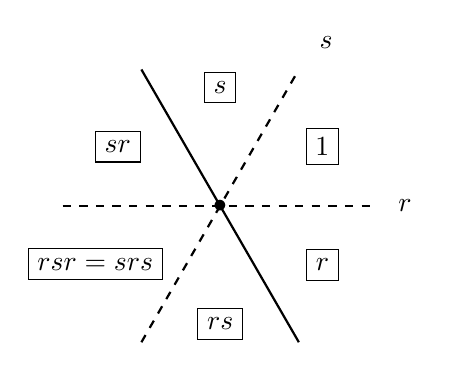
\begin{tikzpicture}
    \draw[thick,dashed] (180:2) to (0:2) node[label=right:{$r$}]{};
    \draw[thick,dashed] (-120:2) to (60:2) node[label=above right:{$s$}]{};
    \draw[thick] (-60:2) to (120:2);
    \node at (0,0) {$\bullet$};
    \node[draw] at (30:1.5) {$1$};
    \node[draw] at (90:1.5) {$s$};
    \node[draw] at (150:1.5) {$sr$};
    \node[draw] at (-30:1.5) {$r$};
    \node[draw] at (-90:1.5) {$rs$};
    \node[draw] at (-155:1.75) {$rsr=srs$};
  \end{tikzpicture}
\] If we start with chamber \(1\) and keep reflecting across mirrors, we
keep getting products of more and more generators until we reach the
diametrically opposite chamber, which corresponds to the so-called
``long word'' in our finite reflection group. In this case, the long
word is \(rsr = srs\).

(Fanatical devotees will also note that this equation is the
``Yang-Baxter equation'' mentioned in \protect\hyperlink{week261}{``Week
261''}.)

Now, Coxeter thought about all this stuff, and he realized that it was
nice to introduce a polytope with one face for each chamber --- in this
case, just a hexagon: \[
  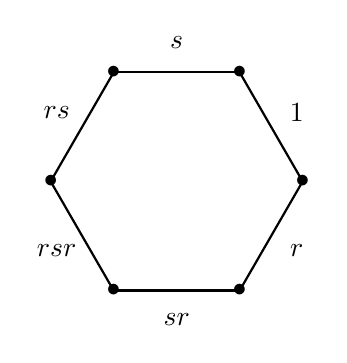
\begin{tikzpicture}[scale=0.8]
    \foreach \a in {0,60,120,180,240,300}{
      \node at (\a:2) {$\bullet$};
      \draw[thick] (\a:2) to ({\a+60}:2);
    };
    \node at (30:2.2) {$1$};
    \node at (90:2.2) {$s$};
    \node at (150:2.2) {$rs$};
    \node at (-30:2.2) {$r$};
    \node at (-90:2.2) {$sr$};
    \node at (-150:2.2) {$rsr$};
  \end{tikzpicture}
\] This is called the ``Coxeter complex'' of our finite reflection
group. Our finite reflection group acts on it, and it acts on the faces
in a free and transitive way.

But, you'll note we started with the symmetry group of an equilateral
triangle, and wound up with a hexagon! What happened?

The quick way to say it is this: combinatorially speaking, the hexagon
is the
``\href{http://en.wikipedia.org/wiki/Barycentric_subdivision}{barycentric
subdivision}'' of our original triangle. Not the inside of the triangle
--- just its surface, or boundary! The boundary of the triangle is a
simplicial complex made of 3 vertices and 3 edges: \[
  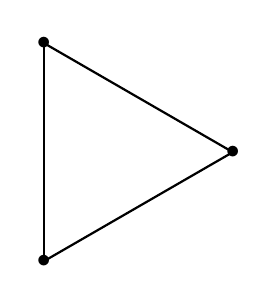
\begin{tikzpicture}[scale=0.8]
    \foreach \a in {0,120,240}{
      \node at (\a:2) {$\bullet$};
      \draw[thick] (\a:2) to ({\a+120}:2);
    };
  \end{tikzpicture}
\] so if we barycentrically subdivide it, we get 6 vertices and 6 edges:
\[
  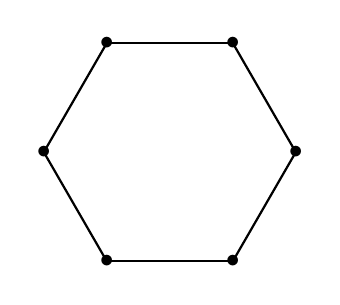
\begin{tikzpicture}[scale=0.8]
    \foreach \a in {0,60,120,180,240,300}{
      \node at (\a:2) {$\bullet$};
      \draw[thick] (\a:2) to ({\a+60}:2);
    };
  \end{tikzpicture}
\] and that's our hexagon --- drawn puffed out a bit, just for the sake
of prettiness.

If this seems bizarre --- and it probably does, given how lousy these
pictures are --- I urge you to try the next example on your own. Take
the symmetry group of the regular tetrahedron, also known as \(S_4\),
the group of permutations of 4 things. Show it's generated by three
reflections \(r,s,t\) with relations \[
  \begin{gathered}
    r^2 = s^2 = t^2 = 1
  \\(rs)^3 = (st)^3 = 1
  \\rt = tr
  \end{gathered}
\] We can summarize these with the following Coxeter diagram: \[
  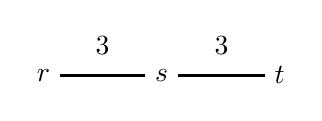
\begin{tikzpicture}
    \node (r) at (0,0) {$r$};
    \node (s) at (1.5,0) {$s$};
    \node (t) at (3,0) {$t$};
    \draw[thick] (r) to node[label=above:{$3$}]{} (s) to node[label=above:{$3$}]{} (t);
  \end{tikzpicture}
\] Draw all mirrors corresponding to reflections in \(S_4\), and show
they chop 3d space into 24 chambers, one for each element of \(S_4\).
Then, barycentrically subdivide the boundary of the tetrahedron and
check that the resulting ``Coxeter complex'' has 24 faces, one inside
each chamber.

Anyway, one thing Tits did is realize how these Coxeter complexes show
up in the geometry of the \emph{Lie groups}, or more generally
\emph{algebraic groups}, associated to Dynkin diagrams.

For example, if I take this guy: \[
  \begin{tikzpicture}
    \node (r) at (0,0) {$r$};
    \node (s) at (2,0) {$s$};
    \draw[thick] (r) to node[label=above:{$3$}]{} (s);
  \end{tikzpicture}
\] and remove some of the labels, I get the so-called \(\mathrm{A}_2\)
Dynkin diagram: \[
  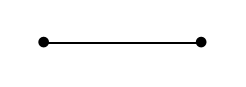
\begin{tikzpicture}
    \node at (0,0) {$\bullet$};
    \node at (2,0) {$\bullet$};
    \draw[thick] (0,0) to (2,0);
  \end{tikzpicture}
\] which corresponds to the Lie group \(\mathrm{PSL}(3)\). And, this is
the group of symmetries of projective plane geometry! Each dot in the
Dynkin corresponds to a ``type of figure'': \[
  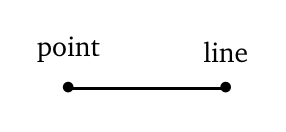
\begin{tikzpicture}
    \node[label=above:{point}] at (0,0) {$\bullet$};
    \node[label=above:{line}] at (2,0) {$\bullet$};
    \draw[thick] (0,0) to (2,0);
  \end{tikzpicture}
\] and the edge corresponds to an ``incidence relation'': in projective
plane geometry, a point can lie on a line. This shape, which we've seen
before: \[
  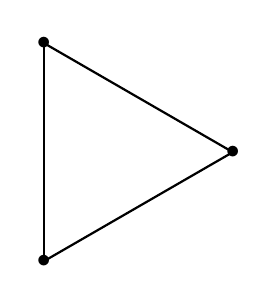
\begin{tikzpicture}[scale=0.8]
    \foreach \a in {0,120,240}{
      \node at (\a:2) {$\bullet$};
      \draw[thick] (\a:2) to ({\a+120}:2);
    };
  \end{tikzpicture}
\] is then revealed to stand for a configuration of 3 points and 3
lines, satisfying incidence relations obvious from the picture. To put
points and lines on an equal footing, we switch to the the Coxeter
complex: \[
  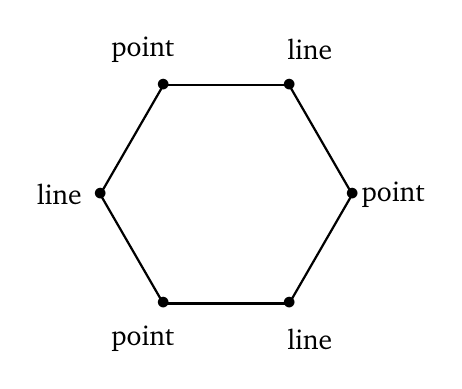
\begin{tikzpicture}[scale=0.8]
    \foreach \a in {0,60,120,180,240,300}{
      \node at (\a:2) {$\bullet$};
      \draw[thick] (\a:2) to ({\a+60}:2);
    };
    \node at (0:2.65) {point};
    \node at (60:2.65) {line};
    \node at (120:2.65) {point};
    \node at (180:2.65) {line};
    \node at (240:2.65) {point};
    \node at (300:2.65) {line};
  \end{tikzpicture}
\] where now the vertices represent ``figures'' and the edges represent
``incidence relations''. It turns out that inside any projective plane,
we can find lots of configurations like this: 3 points and 3 lines, each
pair of points lying on one of the lines, and each pair of lines
intersecting in a point. Such a configuration is called an
``apartment''.

If we take all the apartments coming from a projective plane, they form
a simplicial complex called a ``building''. And this generalizes to any
geometry corresponding to any sort of Dynkin diagram. The building knows
everything about the geometry: all the figures, all the incidence
relations.

And that's all I have time for now, but it's just the beginning of the
marvelous theory Jacques Tits worked out.

\begin{center}\rule{0.5\linewidth}{0.5pt}\end{center}

\textbf{Addenda:} At least on Titan, tholins seem to be a complex brew
of compounds made by irradiation of molecular nitrogen and methane in
the upper atmosphere. The same sort of compounds could be an early
chemical step in the formation of life on Earth --- that's one reason
I'm interested. They're related to PAHs, or ``polycyclic aromatic
hydrocarbons'', which are ubiquitous in outer space --- I wrote about
those back in \protect\hyperlink{week258}{``Week 258''}. I guess the
main difference is that tholins contain nitrogen!

I found some more information on tholins here:

\begin{enumerate}
\def\labelenumi{\arabic{enumi})}
\setcounter{enumi}{15}
\tightlist
\item
  J. H. Waite, Jr., et al, ``The process of tholin formation in Titan's
  upper atmosphere'', \emph{Science} \textbf{316} (2007), 870--875.
\end{enumerate}

Here's a picture of how tholins get made, from this paper:
\[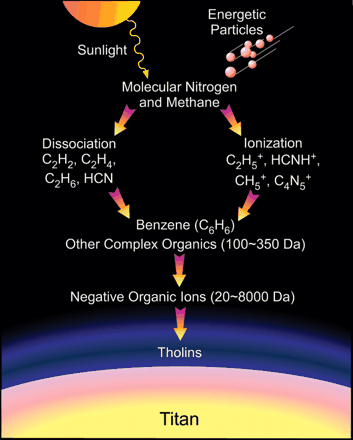
\includegraphics[max width=0.65\linewidth]{../images/titan_tholins.png}\]

You can see more discussion and also \emph{questions I'm dying to know
the answers to} over at the
\href{http://golem.ph.utexas.edu/category/2008/04/this_weeks_finds_in_mathematic_24.html}{\(n\)-Category
Café}. Whenever I write This Week's Finds, I come up with lots of
questions. If you can help me with some of these, I'll be really
grateful.

\begin{center}\rule{0.5\linewidth}{0.5pt}\end{center}

\begin{quote}
\emph{It was technical --- there was no way to avoid it. But it was a
wonderful thing. We'd finally busted it. But then, just before we were
about to submit the paper, Walter noticed a mistake.}

--- John Thompson
\end{quote}



\hypertarget{week264}{%
\section{May 18, 2008}\label{week264}}

Here's a puzzle. Guess the next term of this sequence:
\[1, 1, 2, 3, 4, 5, 6, \ldots\] and then guess the \emph{meaning} of
this sequence! I'll give away the answer after telling you about
Coleman's videos on quantum field theory and an amazing result on the
homotopy groups of spheres.

But first\ldots{} the astronomy picture of the day.

The Eaton Collection at UC Riverside may be the world's best library of
science fiction:

\begin{enumerate}
\def\labelenumi{\arabic{enumi})}
\tightlist
\item
  The Eaton Collection of Science Fiction, Fantasy, Horror and Utopian
  Literature, \texttt{http://eaton-collection.ucr.edu/}.
\end{enumerate}

Right now my wife Lisa Raphals is attending a conference there on the
role of Mars in SF, called ``Chronicling Mars''. Gregory Benford,
Frederik Pohl, Greg Bear, David Brin, Kim Stanley Robinson and even Ray
Bradbury are all there! But for some reason I'm staying home working on
This Week's Finds. I'd say that shows true devotion --- or maybe just
stupidity.

Anyway, in honor of the occasion, here's an incredible closeup of a
crater on Mars' moon Phobos:
\[\href{http://apod.nasa.gov/apod/ap080410.html}{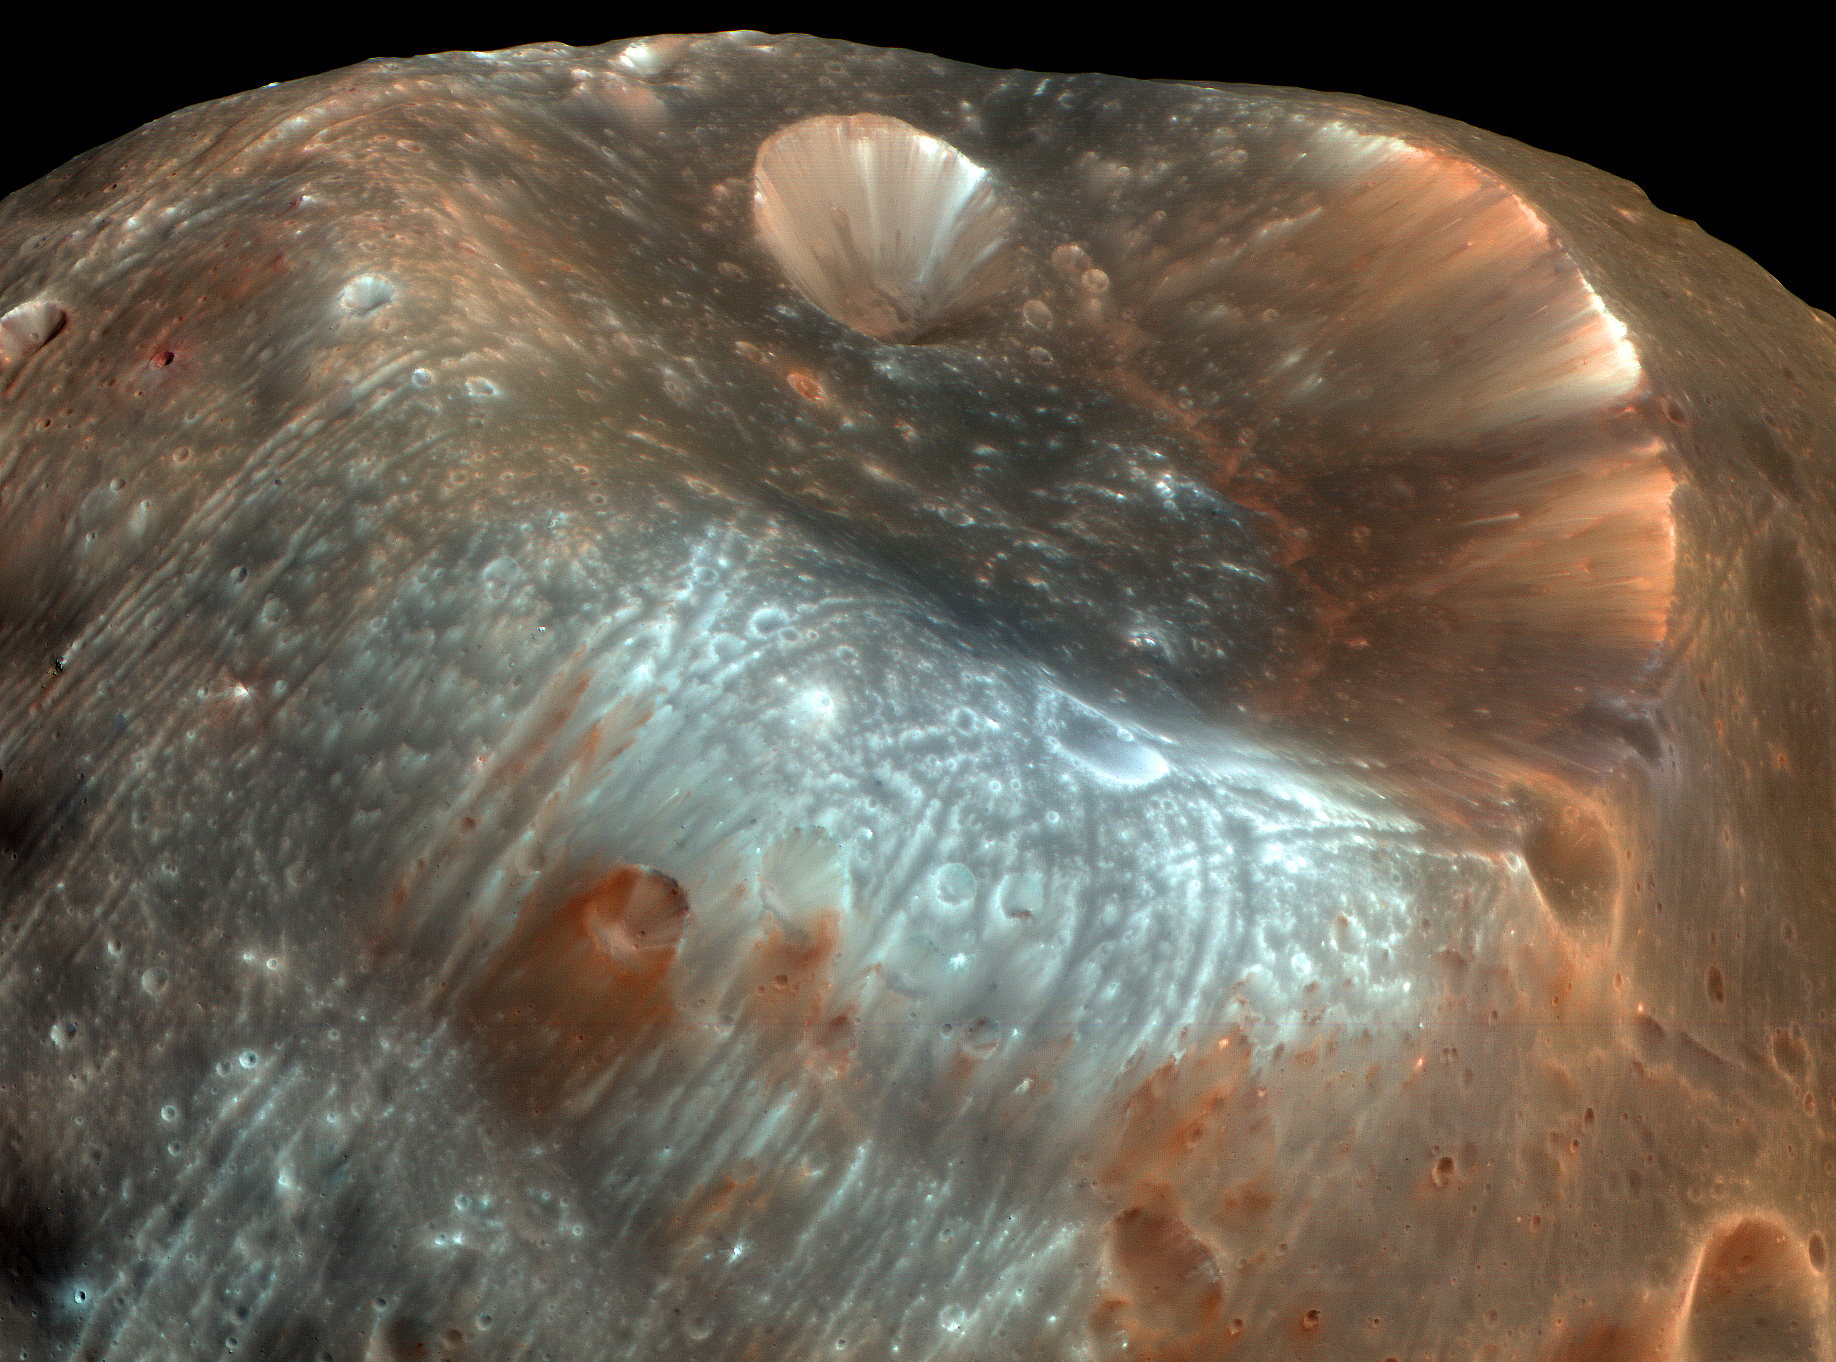
\includegraphics[max width=0.65\linewidth]{../images/phobos.jpg}}\]

\begin{enumerate}
\def\labelenumi{\arabic{enumi})}
\setcounter{enumi}{1}
\tightlist
\item
  Astronomy Picture of the Day, ``Stickney Crater'',
  \texttt{http://apod.nasa.gov/apod/ap080410.html}
\end{enumerate}

It's another great example of how machines in space now deliver many
more thrills per buck than the old-fashioned approach using canned
primates. This photo was taken by HiRISE, the High Resolution Imaging
Science Experiment --- the same satellite that took the stunning photos
of Martian dunes which graced \protect\hyperlink{week262}{``Week 262''}.

Mars has two moons, Phobos and the even tinier Deimos. Their names mean
``fear'' and ``dread'' in Greek, since in Greek mythology they were sons
of Mars (really Ares), the god of war.

Interestingly, Kepler predicted that Mars had two moons before they were
seen. This sounds impressive, but it was simple interpolation, since
Earth has 1 moon and Jupiter has 4. Or at least Galileo saw 4 --- now we
know there are a lot more.

Phobos is only 21 kilometers across, and the big crater you see here -
Stickney Crater --- is about 9 kilometers across. That's almost half the
size of the whole moon! The collision that created it must have almost
shattered Phobos.

Phobos is so light --- just twice the density of water --- that people
once thought it might be hollow. This now seems unlikely, though it's
been the premise of a few SF stories. It's more likely that Phobos is a
loosely packed pile of carbonaceous chondrites captured from the
asteroid belt.

Phobos orbits so close to Mars that it zips around once every 8 hours,
faster than Mars itself rotates! Oddly, in 1726 Jonathan Swift wrote
about two moons of Mars in his novel ``Gulliver's Travels'' --- and he
guessed that the inner one orbited Mars every 10 hours.

Gravitational tidal forces are dragging Phobos down, so in only 10
million years it'll either crash or --- more likely --- be shattered by
tidal forces and form a ring of debris.

So, enjoy it while it lasts.

Anyone who's seriously struggled to master quantum field theory is
likely to have profited from this book:

\begin{enumerate}
\def\labelenumi{\arabic{enumi})}
\setcounter{enumi}{2}
\tightlist
\item
  Sidney Coleman, \emph{Aspects of Symmetry: Selected Erice Lectures},
  Cambridge U. Press, Cambridge, 1988.
\end{enumerate}

It's brimming with wisdom and humor. You should have already encountered
quantum field theory before trying it: what you'll get are deeper
insights.

But what if you're just getting started?

Sidney Coleman, recently deceased, was one of the best quantum field
theorists from the heyday of particle physics. As a grad student I took
a course on quantum field theory from Eddie Farhi, who said he based his
class on the notes from Coleman's class at Harvard. So, I've always been
curious about these notes. Now they're available online in handwritten
form:

\begin{enumerate}
\def\labelenumi{\arabic{enumi})}
\setcounter{enumi}{3}
\tightlist
\item
  Sidney Coleman, ``lecture notes on quantum field theory'', transcribed
  by Brian Hill,
  \texttt{http://www.damtp.cam.ac.uk/user/dt281/qft/col1.pdf} and
  \texttt{http://www.damtp.cam.ac.uk/user/dt281/qft/col2.pdf}
\end{enumerate}

Someone should LaTeX them up!

Even more fun, you can now see \emph{videos} of Coleman teaching quantum
field theory:

\begin{enumerate}
\def\labelenumi{\arabic{enumi})}
\setcounter{enumi}{4}
\tightlist
\item
  Sidney Coleman, \emph{Physics 253: Quantum Field Theory}, 50 lectures
  recorded 1975--1976,
  \texttt{http://www.physics.harvard.edu/about/Phys253.html}
\end{enumerate}

This is a younger, hipper Coleman than I'd ever seen: long-haired,
sometimes puffing on a cigarette between sentences. He begins by saying
``Umm\ldots{} this is Physics 253, a course in relativistic quantum
mechanics. My name is Sidney Coleman. The apparatus you see around you
is part of a CIA surveillance project.''

I wish I'd had access to these when I was a kid!

Now for some miraculous math. Daniel Moskovich kindly pointed out a
paper that describes all the homotopy groups of the \(2\)-sphere, and I
want to summarize the main result.

I explained the idea of homotopy groups back in
\protect\hyperlink{week102}{``Week 102''}. Very roughly, the \(n\)th
homotopy group of a space \(X\), usually denoted \(\pi_n(X)\), is the
set of ways you can map an \(n\)-sphere into that space, where we count
two ways as the same if you can continuously deform one to the other. If
a space has holes, homotopy groups are one way to detect those holes.

Homotopy groups are notoriously hard to compute --- so even for so
humble a space as the \(2\)-sphere, \(S^2\), there's a sense in which
``nobody knows'' all its homotopy groups. People know the first 64,
though. Here are a few: \[
  \begin{aligned}
    \pi_1(S^2) &= 0
  \\\pi_2(S^2) &= \mathbb{Z}
  \\\pi_3(S^2) &= \mathbb{Z}
  \\\pi_4(S^2) &= \mathbb{Z}/2
  \\\pi_5(S^2) &= \mathbb{Z}/2
  \\\pi_6(S^2) &= \mathbb{Z}/4 \times \mathbb{Z}/3
  \\\pi_7(S^2) &= \mathbb{Z}/2
  \\\pi_8(S^2) &= \mathbb{Z}/2
  \\\pi_9(S^2) &= \mathbb{Z}/3
  \\\pi_{10}(S^2) &= \mathbb{Z}/3 \times \mathbb{Z}/5
  \\\pi_{11}(S^2) &= \mathbb{Z}/2
  \\\pi_{12}(S^2) &= \mathbb{Z}/2 \times \mathbb{Z}/2
  \\\pi_{13}(S^2) &= \mathbb{Z}/2 \times \mathbb{Z}/2 \times \mathbb{Z}/3
  \\\pi_{14}(S^2) &= \mathbb{Z}/2 \times \mathbb{Z}/2 \times \mathbb{Z}/4 \times \mathbb{Z}/3 \times \mathbb{Z}/7
  \\\pi_{15}(S^2) &= \mathbb{Z}/2 \times \mathbb{Z}/2
  \end{aligned}
\] Apart from the fact that they're all abelian groups, all finite
except for the first two, it's hard to spot any pattern!

In fact there's a majestic symphony of patterns in the homotopy groups
of spheres, starting from ones that are easy to explain and working on
up to those that push the frontiers of mathematics, like elliptic
cohomology. But, many of these patterns are too complex for present-day
mathematics until we use some tricks to ``water down'' or simplify the
homotopy groups.

So, what people often do first is take the limit of \(\pi_{n+k}(S^n)\)
as \(n \to \infty\), getting what's called the \(k\)th ``stable''
homotopy group of spheres. It's a wonderful but well-understood fact
that these limits really exist. But so far, even these are too
complicated to understand until we work ``at a prime \(p\)''. This means
that we take the \(k\)th stable homotopy group of spheres and see which
groups of the form \(\mathbb{Z}/p^n\) show up in it. For example,
\[\pi_{14}(S^2) = \mathbb{Z}/2 \times \mathbb{Z}/2 \times \mathbb{Z}/4 \times \mathbb{Z}/3 \times \mathbb{Z}/7\]
but if we work ``at the prime \(2\)'' we just see the
\(\mathbb{Z}/2 \times \mathbb{Z}/2 \times \mathbb{Z}/4\).

After all this data processing, we get some astounding pictures:
\[\href{http://www.math.cornell.edu/~hatcher/stemfigs/stems.html}{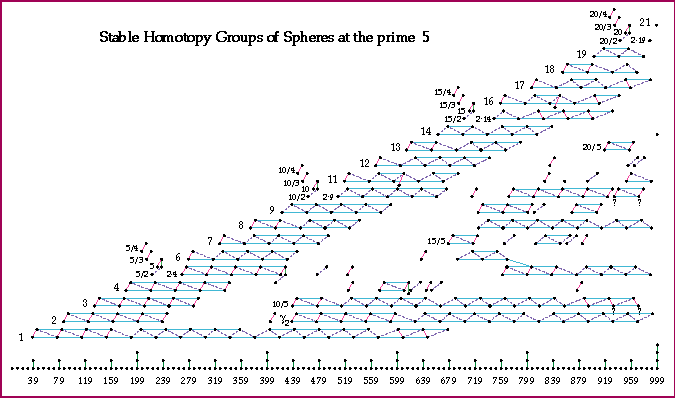
\includegraphics[max width=0.65\linewidth]{../images/stable_homotopy_groups_hatcher.png}}\]
This picture summarizes the first 999 stable homotopy groups of spheres
at the prime \(5\). To understand exactly what it means, read this:

\begin{enumerate}
\def\labelenumi{\arabic{enumi})}
\setcounter{enumi}{5}
\tightlist
\item
  Allen Hatcher, ``Stable homotopy groups of spheres'',
  \texttt{http://www.math.cornell.edu/\textasciitilde{}hatcher/stemfigs/stems.html}
\end{enumerate}

Order teetering on the brink of chaos! If you're brave, you can learn
more about this stuff here:

\begin{enumerate}
\def\labelenumi{\arabic{enumi})}
\setcounter{enumi}{6}
\tightlist
\item
  Douglas C. Ravenel, \emph{Complex Cobordism and Stable Homotopy Groups
  of Spheres}, AMS, Providence, Rhode Island, 2003.
\end{enumerate}

If you're less brave, I strongly suggest starting here:

\begin{enumerate}
\def\labelenumi{\arabic{enumi})}
\setcounter{enumi}{7}
\tightlist
\item
  Wikipedia, ``Homotopy groups of spheres'',
  \texttt{http://en.wikipedia.org/wiki/Homotopy\_groups\_of\_spheres}
\end{enumerate}

But now, I want to talk about an amazing paper that pursues a very
different line of attack. It gives a beautiful description of \emph{all}
the homotopy groups of \(S^2\), in terms of braids:

\begin{enumerate}
\def\labelenumi{\arabic{enumi})}
\setcounter{enumi}{8}
\tightlist
\item
  A. Berrick, F. R. Cohen, Y. L. Wong and J. Wu, ``Configurations,
  braids and homotopy groups'', \emph{J. Amer. Math. Soc.} \textbf{19}
  (2006), 265--326. Also available at
  \texttt{http://www.math.nus.edu.sg/\textasciitilde{}matwujie/BCWWfinal.pdf}
\end{enumerate}

For this you need to realize that for any \(n\), there's a group \(B_n\)
whose elements are \(n\)-strand braids. For example, here's an element
of \(B_3\): \[
  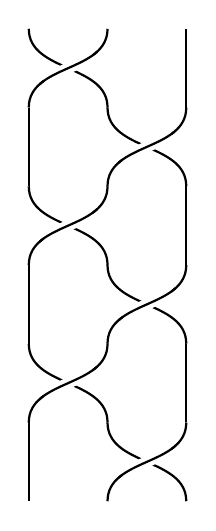
\begin{tikzpicture}
    \begin{knot}[clip width=5]
      \strand[thick] (1,0)
        to [out=down,in=up] (0,-1);
      \strand[thick] (0,0)
        to [out=down,in=up] (1,-1);
      \strand[thick] (2,0) to (2,-1);
    \end{knot}
    \begin{scope}[shift={(1,-1)}]
      \begin{knot}[clip width=5]
        \strand[thick] (1,0)
          to [out=down,in=up] (0,-1);
        \strand[thick] (0,0)
          to [out=down,in=up] (1,-1);
        \strand[thick] (-1,0) to (-1,-1);
      \end{knot}
    \end{scope}
    \begin{scope}[shift={(0,-2)}]
      \begin{knot}[clip width=5]
        \strand[thick] (1,0)
          to [out=down,in=up] (0,-1);
        \strand[thick] (0,0)
          to [out=down,in=up] (1,-1);
        \strand[thick] (2,0) to (2,-1);
      \end{knot}
    \end{scope}
    \begin{scope}[shift={(1,-3)}]
      \begin{knot}[clip width=5]
        \strand[thick] (1,0)
          to [out=down,in=up] (0,-1);
        \strand[thick] (0,0)
          to [out=down,in=up] (1,-1);
        \strand[thick] (-1,0) to (-1,-1);
      \end{knot}
    \end{scope}
    \begin{scope}[shift={(0,-4)}]
      \begin{knot}[clip width=5]
        \strand[thick] (1,0)
          to [out=down,in=up] (0,-1);
        \strand[thick] (0,0)
          to [out=down,in=up] (1,-1);
        \strand[thick] (2,0) to (2,-1);
      \end{knot}
    \end{scope}
    \begin{scope}[shift={(1,-5)}]
      \begin{knot}[clip width=5]
        \strand[thick] (1,0)
          to [out=down,in=up] (0,-1);
        \strand[thick] (0,0)
          to [out=down,in=up] (1,-1);
        \strand[thick] (-1,0) to (-1,-1);
      \end{knot}
    \end{scope}
  \end{tikzpicture}
\] I actually talked about this specific braid back in
\protect\hyperlink{week233}{``Week 233''}. But anyway, we count two
braids as the same if you can wiggle one around until it looks like the
other without moving the ends at the top and bottom --- which you can
think of as nailed to the ceiling and floor.

How do braids become a group? Easy: we multiply them by putting one on
top of the other. For example, this braid: \[
  \raisebox{2.6em}{$A=$}\quad
  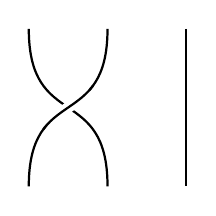
\begin{tikzpicture}
    \begin{knot}[clip width=5]
      \strand[thick] (1,0)
        to [out=down,in=up,looseness=1.5] (0,-2);
      \strand[thick] (0,0)
        to [out=down,in=up,looseness=1.5] (1,-2);
      \strand[thick] (2,0) to (2,-2);
    \end{knot}
  \end{tikzpicture}
\] times this one: \[
  \raisebox{2.6em}{$B=$}\quad
  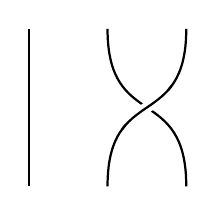
\begin{tikzpicture}
    \begin{knot}[clip width=5]
      \strand[thick] (1,0)
        to [out=down,in=up,looseness=1.5] (0,-2);
      \strand[thick] (0,0)
        to [out=down,in=up,looseness=1.5] (1,-2);
      \strand[thick] (-1,0) to (-1,-2);
    \end{knot}
  \end{tikzpicture}
\] equals this: \[
  \raisebox{2.6em}{$AB=$}\quad
  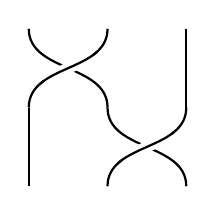
\begin{tikzpicture}
    \begin{knot}[clip width=5]
      \strand[thick] (1,0)
        to [out=down,in=up] (0,-1);
      \strand[thick] (0,0)
        to [out=down,in=up] (1,-1);
      \strand[thick] (2,0) to (2,-1);
    \end{knot}
    \begin{scope}[shift={(1,-1)}]
      \begin{knot}[clip width=5]
        \strand[thick] (1,0)
          to [out=down,in=up] (0,-1);
        \strand[thick] (0,0)
          to [out=down,in=up] (1,-1);
        \strand[thick] (-1,0) to (-1,-1);
      \end{knot}
    \end{scope}
  \end{tikzpicture}
\] and in fact the big one I showed you earlier is \((AB)^3\).

As you let your eye slide from the top to the bottom of a braid, the
strands move around. We can visualize their motion as a bunch of points
running around the plane, never bumping into each other. This gives an
interesting way to generalize the concept of a braid! Instead of points
running around the plane, we can have points running around \(S^2\), or
some other surface \(X\). So, for any surface \(X\) and any number \(n\)
of strands, we get a ``surface braid group'', called \(B_n(X)\).

As I hinted in \protect\hyperlink{week261}{``Week 261''}, these surface
braid groups have cool relationships to Dynkin diagrams. I urged you to
read this paper, and I'll urge you again:

\begin{enumerate}
\def\labelenumi{\arabic{enumi})}
\setcounter{enumi}{9}
\tightlist
\item
  Daniel Allcock, ``Braid pictures for Artin groups'', available as
  \href{http://arxiv.org/abs/math.GT/9907194}{\texttt{arXiv:math.GT/9907194}}.
\end{enumerate}

But for now, we just need the ``spherical braid group'' \(B_n(S^2)\)
together with the usual braid group \(B_n\).

Let's say a braid is ``Brunnian'' if when you remove any one strand, the
remaining braid becomes the identity: you can straighten out all the
remaining strands to make them vertical. It's a fun little exercise to
check that Brunnian braids form a subgroup of all braids. So, we have an
\(n\)-strand Brunnian braid group \(BB_n\).

The same idea works for braids on other surface, like the \(2\)-sphere.
So, we also have an \(n\)-strand \emph{spherical} Brunnian braid group
\(BB_n(S^2)\).

Now, there's obvious map \[B_n \to B_n(S^2)\] Why? An element of \(B_n\)
describes the motion of a bunch of points running around the plane, but
the plane sits inside the \(2\)-sphere: the \(2\)-sphere is just the
plane with an extra point tacked on. So, an ordinary braid gives a
spherical braid.

This map clearly sends Brunnian braids to spherical Brunnian braids, so
we get a map \[f\colon BB_n \to BB_n(S^2)\] And now we're ready for the
shocking theorem of Berrick, Cohen, Wong and Wu:

\begin{quote}
\textbf{Theorem:} For \(n > 3\), \(\pi_n(S^2)\) is \(BB_n(S^2)\) modulo
the image of \(f\).
\end{quote}

In something more like plain English: when \(n\) is big enough, the
\(n\)th homotopy group of the \(2\)-sphere consists of spherical
Brunnian braids modulo ordinary Brunnian braids!

Zounds! What do the homotopy groups of \(S^2\) have to do with braids?
It's not supposed to be obvious! The proof of this result is long and
deep, making use of flows on metric spaces, and also the fact that all
the Brunnian braid groups \(BB_n\) fit together into a ``simplicial
group'' whose \(n\)th homology is the \(n\)th homotopy group of \(S^2\).
I'd love to understand all this stuff, but I don't yet.

This result doesn't instantly help us ``compute'' the homotopy groups of
\(S^2\) --- at least not in the sense of writing them down as a product
of groups like \(\mathbb{Z}/p^n\). But, it gives a new view of these
homotopy groups, and there's no telling where this might lead.

When I was first getting ready to write this article, I was also going
to tell you about some amazing descriptions of the homotopy groups of
the \emph{3-sphere}, due to Wu.

However, I later realized --- first to my shock, and then my
embarrassment for not having known it already --- that the \(n\)th
homotopy group of \(S^3\) is \emph{the same} as the \(n\)th homotopy
group of \(S^2\), at least for \(n > 2\). Do you see why?

Given this, it turns out that Wu's results are predecessors of the
theorem just stated, a bit more combinatorial and less ``geometric''.
Wu's results appeared here:

\begin{enumerate}
\def\labelenumi{\arabic{enumi})}
\setcounter{enumi}{11}
\item
  Jie Wu, ``On combinatorial descriptions of the homotopy groups of
  certain spaces'', \emph{Math. Proc. Camb. Phil. Soc.} \textbf{130}
  (2001), 489--513. Also available at
  \texttt{http://www.math.nus.edu.sg/\textasciitilde{}matwujie/newnewpis\_3.pdf}

  Jie Wu, ``A braided simplicial group'', \emph{Proc. London Math. Soc.}
  \textbf{84} (2002), 645--662. Also available at
  \texttt{http://www.math.nus.edu.sg/\textasciitilde{}matwujie/wgroup05-19-01.pdf}
\end{enumerate}

and there's a nice summary of these results on his webpage:

\begin{enumerate}
\def\labelenumi{\arabic{enumi})}
\setcounter{enumi}{12}
\tightlist
\item
  Jie Wu, ``2.1 Homotopy groups and braids'', halfway down the page at
  \texttt{http://www.math.nus.edu.sg/\textasciitilde{}matwujie/Research2.html}
\end{enumerate}

See also this expository paper:

\begin{enumerate}
\def\labelenumi{\arabic{enumi})}
\setcounter{enumi}{13}
\tightlist
\item
  Fred R. Cohen and Jie Wu, ``On braid groups and homotopy groups'',
  \emph{Geometry \& Topology Monographs} \textbf{13} (2008), 169--193.
  Also available at
  \texttt{http://www.math.nus.edu.sg/\textasciitilde{}matwujie/cohen.wu.GT.revised.29.august.2007.pdf}
\end{enumerate}

Next I want to talk about puzzle mentioned at the start of this Week's
Finds\ldots{} but first I should answer the puzzle I just raised. Why do
the homotopy groups of \(S^2\) match those of \(S^3\) after a while?
Because of the Hopf fibration! This is a fiber bundle with \(S^3\) as
total space, \(S^2\) as base space and \(S^1\) as fiber:
\[S^1 \to S^3 \to S^2\] Like any fiber bundle, it gives a long exact
sequence of homotopy groups as explained in
\protect\hyperlink{week151}{``Week 151''}:
\[\ldots \to \pi_n(S^1) \to \pi_n(S^3) \to \pi_n(S^2) \to \pi_{n-1}(S^1) \to \ldots\]
but the homotopy groups of \(S^1\) vanishes after the first, so we get
\[\ldots \to 0 \to \pi_n(S^3) \to \pi_n(S^2) \to 0 \to \ldots\] for
\(n > 2\), which says that \[\pi_n(S^3) \cong \pi_n(S^2)\]

Okay, now for this mysterious sequence: \[1, 1, 2, 3, 4, 5, 6, \ldots\]
The next term is obviously 7. If you guessed anything else, you were
over-analyzing. So the real question is: why the funny ``hiccup'' at the
beginning? Why the repeated 1?

You'll find two explanations of this sequence in Sloane's Online
Encyclopedia of Integer Sequences, but neither of them is the reason
James Dolan and I ran into it. We were learning about theta
functions\ldots{}

Say you have a torus. Then the complex line bundles over it are
classified by an integer called their ``first Chern number''. In some
sense, this integer this measures how ``twisted'' the bundle is. For
example, you can put any connection on the bundle, compute its curvature
\(2\)-form, and integrate it over the torus: up to some constant factor,
you'll get the first Chern number.

A torus is a \(2\)-dimensional manifold, but we can also make it into a
\(1\)-dimensional \emph{complex} manifold, often called an ``elliptic
curve''. In fact we can do this in infinitely many fundamentally
different ways, one for each point in the ``moduli space of elliptic
curves''. I've explained this repeatedly here --- try
\protect\hyperlink{week125}{``Week 125''} for a good starting-point ---
so I won't do so again. The details don't really matter here.

Back to line bundles. If we pick an elliptic curve, we can try to
classify the \emph{holomorphic} complex line bundles over it --- that
is, those where the transition functions are holomorphic (or in other
words, complex-analytic). Here the classification is subtler. It turns
out you need, not just the first Chern number, which is discrete, but
another parameter which can vary in a \emph{continuous} way.

Interestingly, this other parameter can be thought of as just a point on
your elliptic curve! So, an elliptic curve is a space that classifies
holomorphic line bundles over itself --- at least, those with fixed
first Chern number. Curiously circular, eh? This is just one of several
curiously circular classification theorems that happen in this
game\ldots{}

But I'm actually digressing a bit --- I'm having trouble resisting the
temptation to explain everything I've just been learning, since it's so
simple and beautiful. Don't worry --- all you need to know is that
holomorphic line bundles over an elliptic curve are classified by an
integer and some other continuous parameter.

The puzzle then arises: how many holomorphic sections do these line
bundles have? More precisely: what's the \emph{dimension} of the space
of holomorphic sections?

Before I answer this, I can't resist adding that these holomorphic
sections have a long and illustrious history --- they're called ``theta
functions'', and you can learn about them here:

\begin{enumerate}
\def\labelenumi{\arabic{enumi})}
\setcounter{enumi}{14}
\item
  Jun-ichi Igusa, \emph{Theta Functions}, Springer, Berlin, 1972.
\item
  David Mumford, \emph{Tata Lectures on Theta}, 3 volumes, Birkhauser,
  Boston, 1983--1991.
\end{enumerate}

They're important in geometric quantization, where holomorphic sections
of line bundles describe states of quantum systems, and the reciprocal
of the first Chern number is proportional to Planck's constant. In fact,
I first ran into theta functions years ago, when trying to quantize a
black hole --- see the end of \protect\hyperlink{week112}{``Week 112''}
for more details.

But anyway, here's the answer to the puzzle. The dimension turns out not
to depend on the continuous parameter labelling our line bundle, but
only on its first Chern number. If that number is negative, the
dimension is \(0\). But if it's \(0,1,2,3,4,5,6\) and so on, the
dimension goes like this: \[1, 1, 2, 3, 4, 5, 6,\ldots\] Now, this
sequence is fairly weird, because of the extra ``\(1\)'' at the
beginning. I hadn't noticed this back when I was quantizing black holes,
because the extra ``\(1\)'' happens for first Chern number zero, which
would correspond to Planck's constant being \emph{infinite}. But now
that I'm just thinking about math, it sticks out like a sore thumb!

It's got to be right, since the line bundle with first Chern number zero
is the trivial bundle, its sections are just functions, and the only
holomorphic functions on a compact complex manifold are constants - so
there's a \(1\)-dimensional space of them. But, it's weird.

Luckily, Jim figured out the explanation for this sequence. First of
all, we can encode it into a power series:
\[1 + x + 2x^2 + 3x^3 + 4x^4 + \ldots\] which we can rewrite as a
rational function:
\[1 + x + 2x^2 + 3x^3 + 4x^4 + \ldots = \frac{1-x^6}{(1-x)(1-x^2)(1-x^3)}\]
Now, the reason for doing this is that we can pick a line bundle of
first Chern number \(1\), say \(L\), and get a line bundle of any Chern
number n by taking the \(n\)th tensor power of \(L\) --- let's call that
\(L^{\otimes n}\). We can multiply a section of \(L^{\otimes n}\) and a
section of \(L^{\otimes m}\) to get a section of \(L^{\otimes(n+m)}\).
So, all these spaces of sections we're studying fit together to form a
commutative graded ring! And, whenever you have a graded ring, it's a
good idea to write down a power series that encodes the dimensions of
each grade, just as we've done above. This is called a ``Poincare
series''.

And, when you have a commutative graded ring with one generator of
degree 1, one generator of degree 2, one generator of degree 3, one
relation of degree 6, and no ``relations between relations'' (or
``syzygies''), its Poincare series will be
\[\frac{1-x^6}{(1-x)(1-x^2)(1-x^3)}\] That's how it always works ---
think about it.

So, it's natural to hope that our ring built from holomorphic sections
of all the line bundles \(L^{\otimes n}\) will have one generator of
degree 1, one of degree 2, one of degree 3, and one relation of degree
6.

And, this seems to be true!

As I mentioned, people usually call these holomorphic sections ``theta
functions''. So, what we're getting is a description of the ring of
theta functions in terms of generators and relations.

How does it work, exactly? Well, I must admit I'm not quite sure. Jim
has some ideas, but it seems I need to do something a bit different to
get his story to work for me. Maybe it goes something like this. We can
write any elliptic curve as the solutions of this equation:
\[y^2 = x^3 + Bx + C\] for certain constants \(B\) and \(C\) that depend
on the elliptic curve. (See \protect\hyperlink{week13}{``Week 13''} and
\protect\hyperlink{week261}{``Week 261''} for details.) Now, this
equation is not homogeneous in the variables \(y\) and \(x\), but we can
think of it as homogeneous in a sneaky sense if we throw in an extra
variable like this: \[y^2 = x^3 + Bxz^4 + Cz^6\] and decree that:

\begin{itemize}
\tightlist
\item
  \(y\) has grade \(3\)
\item
  \(x\) has grade \(2\)
\item
  \(z\) has grade \(1\)
\end{itemize}

Then all the terms in the equation have grade 6. So, we're getting a
commutative graded ring with generators of degree 1, 2, and 3 and a
relation of grade 6. And, I'm hoping this ring consists of algebraic
functions on the total space of some line bundle \(L^*\) over our
elliptic curve. \(z\) should be a function that's linear in the fiber
directions, hence a section of \(L\). \(x\) should be quadratic in the
fiber directions, hence a section of \(L^{\otimes2}\). And \(y\) should
be cubic, hence a section of \(L^{\otimes3}\). If \(L\) has first Chern
number \(1\), I think we're in business.

If anybody knows about this stuff, I'd appreciate corrections or
references.

There's a \emph{lot} more to say about this business\ldots{} because
it's all part of a big story about elliptic curves, theta functions and
modular forms. But, I want to quit here for now.

\begin{center}\rule{0.5\linewidth}{0.5pt}\end{center}

\textbf{Addenda:} I thank David Corfield for pointing out how to get
ahold of Wu's papers free online --- and earlier, for telling me Wu's
combinatorial description of \(\pi_3(S^2)\).

Martin Ouwehand told me that some of Coleman's lecture notes on quantum
field theory are available in TeX here:

\begin{enumerate}
\def\labelenumi{\arabic{enumi})}
\setcounter{enumi}{16}
\tightlist
\item
  Sidney Coleman, \emph{Quantum Field Theory}, first 11 lectures notes
  TeXed by Bryan Gin-ge Chen, available at
  \texttt{http://www.physics.upenn.edu/\textasciitilde{}chb/phys253a/coleman/}
\end{enumerate}

James Dolan pointed out that this article:

\begin{enumerate}
\def\labelenumi{\arabic{enumi})}
\setcounter{enumi}{17}
\tightlist
\item
  Wikipedia, ``Riemann-Roch theorem'',
  \texttt{http://en.wikipedia.org/wiki/Riemann-Roch}
\end{enumerate}

has some very relevant information on the sequence
\[1, 1, 2, 3, 4, 5, 6, \ldots\] though it's phrased not in terms of
``sections of line bundles'', but instead in terms of ``divisors''
(secretly another way of talking about the same thing). Let me quote a
portion, just to whet your interest:

\begin{quote}
We start with a connected compact Riemann surface of genus \(g\), and a
fixed point \(P\) on it. We may look at functions having a pole only at
\(P\). There is an increasing sequence of vector spaces: functions with
no poles (i.e., constant functions), functions allowed at most a simple
pole at \(P\), functions allowed at most a double pole at \(P\), a
triple pole, \ldots{} These spaces are all finite dimensional. In case
\(g = 0\) we can see that the sequence of dimensions starts
\[1, 2, 3, \ldots\] This can be read off from the theory of partial
fractions. Conversely if this sequence starts \[1, 2, \ldots\] then
\(g\) must be zero (the so-called Riemann sphere).

In the theory of elliptic functions it is shown that for \(g = 1\) this
sequence is \[1, 1, 2, 3, 4, 5, \ldots\] and this characterises the case
\(g = 1\). For \(g > 2\) there is no set initial segment; but we can say
what the tail of the sequence must be. We can also see why \(g = 2\) is
somewhat special.

The reason that the results take the form they do goes back to the
formulation (Roch's part) of the {[}Riemann-Roch{]} theorem: as a
difference of two such dimensions. When one of those can be set to zero,
we get an exact formula, which is linear in the genus and the degree
(i.e.~number of degrees of freedom). Already the examples given allow a
reconstruction in the shape
\[\text{dimension} - \text{correction} = \text{degree} - g + 1.\] For
\(g = 1\) the correction is \(1\) for degree \(0\); and otherwise \(0\).
The full theorem explains the correction as the dimension associated to
a further, `complementary' space of functions.
\end{quote}

You can see more discussion of this Week's Finds at the
\href{http://golem.ph.utexas.edu/category/2008/05/this_weeks_finds_in_mathematic_25.html}{\(n\)-Category
Café}.

\begin{center}\rule{0.5\linewidth}{0.5pt}\end{center}

\begin{quote}
\emph{The career of a young theoretical physicist consists of treating
the harmonic oscillator in ever-increasing levels of abstraction.}

--- Sidney Coleman
\end{quote}



\hypertarget{week265}{%
\section{May 25, 2008}\label{week265}}

Today I'd like to talk about the Pythagorean pentagram, Bill Schmitt's
work on Hopf algebras in combinatorics, the magnum opus of Aguiar and
Mahajan, and quaternionic analysis. But first, the astronomy picture of
the week.

I seem to be into moons these days: first Saturn's moon Titan in
\protect\hyperlink{week263}{``Week 263''}, and then Mars' moon Phobos in
\protect\hyperlink{week264}{``Week 264''}. On the cosmic scale, our
Solar System is like our back yard. It may not be important in the grand
scheme of things, but we should get to know it and learn to take care of
it. It's got lots of cool moons. So this week, let's talk about
\href{http://en.wikipedia.org/wiki/Europa_\%28moon\%29}{Europa}:
\[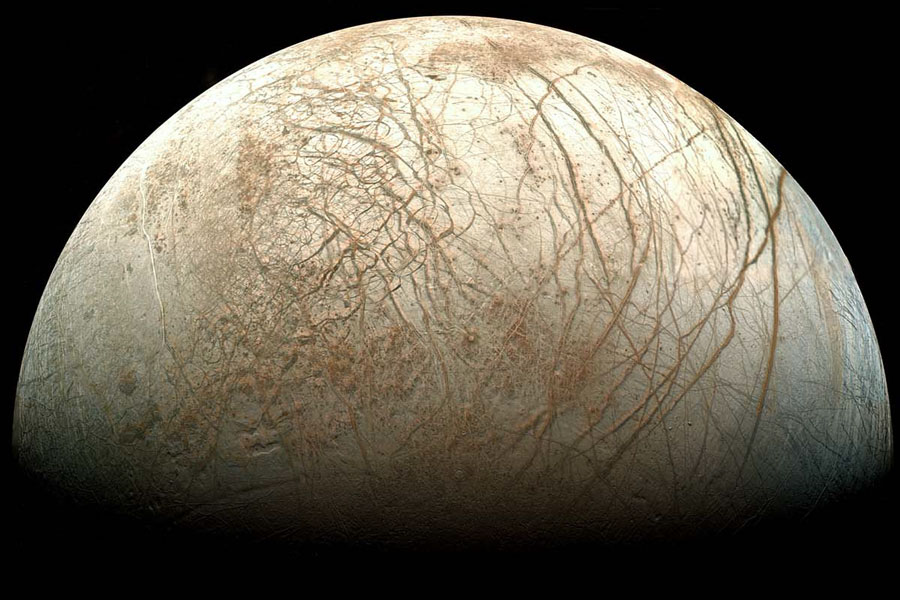
\includegraphics[max width=0.65\linewidth]{../images/europa.jpg}\]

\begin{enumerate}
\def\labelenumi{\arabic{enumi})}
\tightlist
\item
  Astronomy Picture of the Day, ``Gibbous Europa'',
  \texttt{http://antwrp.gsfc.nasa.gov/apod/ap071202.html}
\end{enumerate}

Europa is the fourth biggest moon of Jupiter, the smallest of the four
seen by Galileo. It's 3000 kilometers in diameter, slightly smaller than
our moon, and it zips around Jupiter once every 3.5 of our days, though
it's almost twice as far from Jupiter as our moon is from us.

It looks like a cracked ball of ice, and that's what it is --- at least
near the surface.

Indeed, this ancient impact crater looks like a smashed windshield, or a
frozen lake that's been hit with a sledgehammer:
\[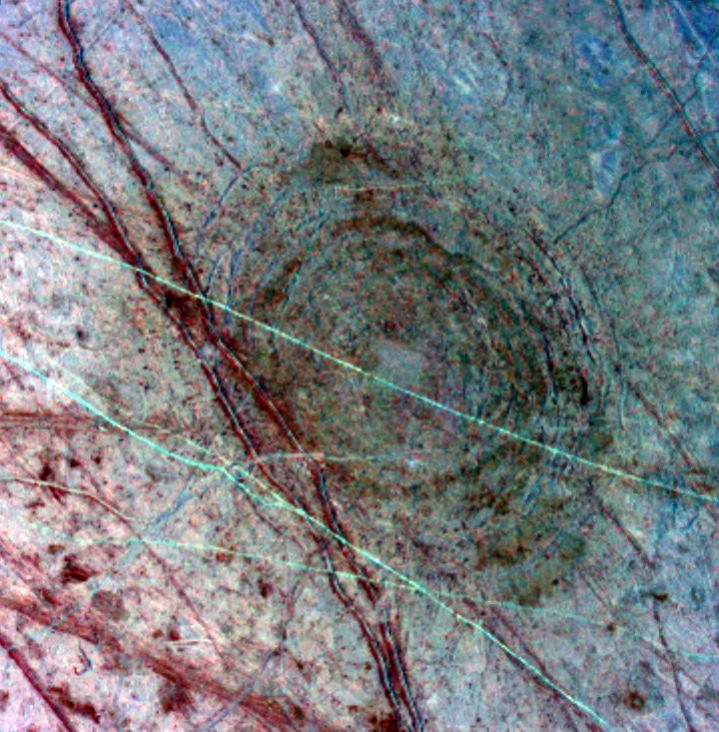
\includegraphics[max width=0.65\linewidth]{../images/europa_impact_crater.jpg}\]

\begin{enumerate}
\def\labelenumi{\arabic{enumi})}
\setcounter{enumi}{1}
\tightlist
\item
  NASA Photojournal, ``Ancient impact basin on Europa'',
  \texttt{http://photojournal.jpl.nasa.gov/catalog/PIA00702}
\end{enumerate}

But this crater, called Tyre, is huge: about as big as the island of
Hawaii, 145 kilometers across! (Beware: this picture is a composite of
three photos taken by the Galileo spacecraft in 1997. It's in false
color designed to show off various structures: the original crater, the
later red cracks, and the blue-green ridges.)

The big question is whether there's liquid water beneath the icy
surface\ldots{} and if so, maybe life? One model of this moon posits a
solid ice crust. Another says there's liquid water too:
\[\href{http://photojournal.jpl.nasa.gov/catalog/PIA01669}{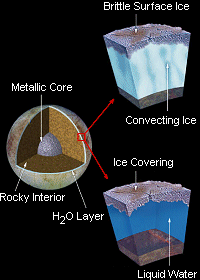
\includegraphics[max width=0.65\linewidth]{../images/europa_models.png}}\]

\begin{enumerate}
\def\labelenumi{\arabic{enumi})}
\setcounter{enumi}{2}
\tightlist
\item
  NASA Photojournal, Model of Europa's subsurface structure,
  \texttt{http://photojournal.jpl.nasa.gov/catalog/PIA01669}
\end{enumerate}

How can we tell? Europa is the \emph{smoothest} of all solid planets and
moons, with lots of cracks and ridges but few remaining craters. This
suggests either an ocean beneath the surface, or at least ice warm
enough to keep convection going. The region called Conamara Chaos looks
like pack ice here on Earth, hinting at liquid water beneath:
\[\href{http://photojournal.jpl.nasa.gov/jpeg/PIA01127.jpg}{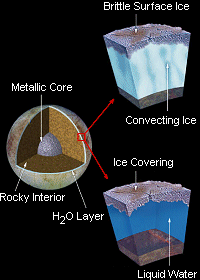
\includegraphics[max width=0.65\linewidth]{../images/europa_models.png}}\]

\begin{enumerate}
\def\labelenumi{\arabic{enumi})}
\setcounter{enumi}{3}
\tightlist
\item
  NASA Photojournal, ``Europa: ice rafting view'',
  \texttt{http://photojournal.jpl.nasa.gov/catalog/PIA01127}
\end{enumerate}

The bluish white areas have been blanketed with ice dust ejected from
far away when an impact formed a crater called
\href{http://en.wikipedia.org/wiki/Pwyll_\%28crater\%29}{Pwyll}. The
reddish brown regions could contain salts or sulfuric acid --- it's hard
to find out using spectroscopy, since there's too much ice.

Another very nice piece of evidence for \emph{salty} liquid water inside
Europa is that the magnetic field of Jupiter induces electric currents
in this moon, which in turn create their own magnetic fields! These
fields were detected when the Galileo probe swooped closest to Europa
back in 2000:

\begin{enumerate}
\def\labelenumi{\arabic{enumi})}
\setcounter{enumi}{4}
\tightlist
\item
  M. G. Kivelson, K. K. Khurana, C. T. Russell, M. Volwerk, R.J. Walker,
  and C. Zimmer, ``Galileo magnetometer measurements: a stronger case
  for a subsurface ocean at Europa'', \emph{Science} \textbf{289}
  (2000), 1340--1343.
\end{enumerate}

At the time, Margaret Kivelson, head of the magnetometer project, said:

\begin{quote}
I think these findings tell us that there is indeed a layer of liquid
water beneath Europa's surface. I'm cautious by nature, but this new
evidence certainly makes the argument for the presence of an ocean far
more persuasive. Jupiter's magnetic field at Europa's position changes
direction every \(5\frac12\) hours. This changing magnetic field can
drive electrical currents in a conductor, such as an ocean. Those
currents produce a field similar to Earth's magnetic field, but with its
magnetic north pole --- the location toward which a compass on Europa
would point --- near Europa's equator and constantly moving. In fact, it
is actually reversing direction entirely every \(5\frac12\) hours.
\end{quote}

A couple weeks ago, another nice piece of evidence was announced: \[
  \begin{gathered}
    \href{http://www.lpi.usra.edu/science/schenk/europaCropCircles/}{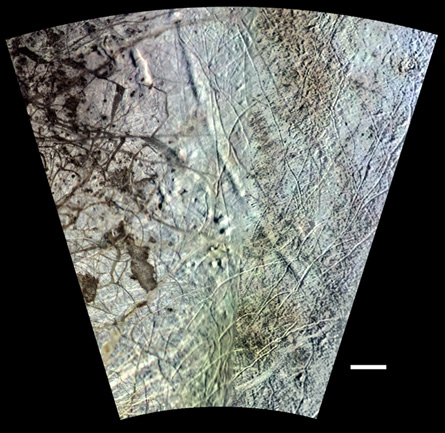
\includegraphics[max width=0.65\linewidth]{../images/europa_polar_wandering_schenk.jpg}}
  \\\text{Scale bar is 100 kilometers long.}
  \\\text{Picture by Paul Schenk, Lunar and Planetary Institute.}
  \end{gathered}
\]

\begin{enumerate}
\def\labelenumi{\arabic{enumi})}
\setcounter{enumi}{5}
\item
  Paul Schenk, Isamu Matsuyama and Francis Nimmo, ``True polar wander on
  Europa from global-scale small-circle depressions'', \emph{Nature}
  \textbf{453} (2008), 368--371.

  Paul Schenk, ``Scars from Europa's polar wandering betray ocean
  beneath'',
  \texttt{http://www.lpi.usra.edu/science/schenk/europaCropCircles/}
\end{enumerate}

There are two arc-shaped depressions exactly opposite each other on
Europa, each hundreds of kilometers long and between \(.3\) and \(1.5\)
kilometers deep. According to the above paper, these scars have just the
right shape to be caused the moon's icy shell rotating a quarter turn
relative to the interior! The authors believe this could happen most
easily if it were floating on an ocean.

If Europa has an ocean under its ice, other questions immediately arise.
How thick is the ice and how deep is the ocean? Some guess 15--30
kilometers of ice atop 100 kilometers of liquid. What keeps it warm?
Heating produced by tidal forces may be the best bet --- radioactivity
from the core contributes just about 100 billion watts, not nearly
enough:

\begin{enumerate}
\def\labelenumi{\arabic{enumi})}
\setcounter{enumi}{6}
\tightlist
\item
  M. N. Ross and G. Schubert, ``Tidal heating in an internal ocean model
  of Europa'', \emph{Nature} \textbf{325} (1987), 133--144.
\end{enumerate}

And then for the really big question: could there be \emph{life} on
Europa? Antarctica has an enormous lake called
\href{http://en.wikipedia.org/wiki/Lake_Vostok}{Lake Vostok} buried
under 4 kilometers of ice, and when people drilled into it they found
all sorts of bizarre life forms that had never been seen before. So,
especially if Europa had been warmer once, it's conceivable that life
might have formed there and survives to this day. Of course, the surface
of Europa makes Antarctica look downright balmy: it's \(-160\) Celsius
at the equator. And liquid water below could be mixed with sulfuric
acid, or lots of nasty salts\ldots{}

Nonetheless, some dream of sending a satellite to Europa, perhaps to
impact it at high velocity and see what's inside, or perhaps to land and
melt down through the ice:

\begin{enumerate}
\def\labelenumi{\arabic{enumi})}
\setcounter{enumi}{7}
\tightlist
\item
  Leslie Mullen, ``Hitting Europa hard (interview of Karl Hibbits)'',
  \emph{Astrobiology Magazine}, May 1, 2006,
  \texttt{http://www.astrobio.net/news/article1944.html}
\end{enumerate}

But these dreams may not come true anytime soon. In 2005, NASA cancelled
its ambitious plans for the Jupiter Icy Moons Orbiter:

\begin{enumerate}
\def\labelenumi{\arabic{enumi})}
\setcounter{enumi}{9}
\tightlist
\item
  Wikipedia, ``Jupiter Icy Moons Orbiter'',
  \texttt{http://en.wikipedia.org/wiki/Jupiter\_Icy\_Moons\_Orbiter}
\end{enumerate}

The U.S. Congress, the National Academy of Sciences, and the NASA
Advisory Committee have all supported a mission to Europa, but NASA has
still not funded this project:

\begin{enumerate}
\def\labelenumi{\arabic{enumi})}
\setcounter{enumi}{10}
\tightlist
\item
  Leonard David, ``Europa mission: lost in NASA budget'',
  \emph{SPACE.com}, February 7, 2006,
  \texttt{http://www.space.com/news/060207\_europa\_budget.html}
\end{enumerate}

Unfortunately, NASA still spends most of its money on expensive manned
missions --- the Buck Rogers approach to space. They think the public
wants the ``glamor'' of manned missions. So, while they just safely
landed the Phoenix spacecraft on Mars, they're also busy struggling to
fix a toilet in near earth orbit, on the International Space Station.

To study the underground ocean of Europa, our best hope may lie with the
European Space Agency's ``Jovian Europa Orbiter'', part of a project
called the Jovian Minisat Explorer:

\begin{enumerate}
\def\labelenumi{\arabic{enumi})}
\setcounter{enumi}{11}
\tightlist
\item
  ESA Science and Technology, ``Jovian Minisat Explorer'',
  \texttt{http://sci.esa.int/science-e/www/object/index.cfm?fobjectid=35982}
\end{enumerate}

This hasn't been funded yet, and there's no telling if it ever will. But
people are already working to make sure Europa doesn't get contaminated
by bacteria from Earth:

\begin{enumerate}
\def\labelenumi{\arabic{enumi})}
\setcounter{enumi}{12}
\tightlist
\item
  National Research Council, ``Preventing the Forward Contamination of
  Europa'', The National Academies Press, Washington, DC, 2000. Also
  available at \texttt{http://www.nap.edu/catalog.php?record\_id=9895}
\end{enumerate}

In fact the US and many other countries are obligated to do this, since
they signed a United Nations treaty that requires it.

The Galileo probe had not been sterilized in a way that would kill
\href{http://en.wikipedia.org/wiki/Extremophile}{extremophiles} ---
organisms that survive extreme conditions. So, the National Research
Council recommended that NASA crash Galileo into Jupiter when its
mission was over, to avoid an accidental collision with Europa. So,
that's what they did! After 14 years of collecting data about Jupiter
and its moons, Galileo crashed into Jupiter and burned up in its
atmosphere on September 21, 2004.

Maybe I'll talk about other moons of Jupiter next week\ldots{} the most
interesting ones besides Europa are volcanic, sulfurous Io and icy
Ganymede, biggest of all.

But now let me turn to the Pythagorean pentagram.

The Pythagoreans --- that strange Greek cult of vegetarian
mathematicians --- were apparently fascinated by the pentagram. Why? I
don't think there's any textual evidence to help us answer this
question, but luckily there's another way to settle it: unsubstantiated
wild guesses!

If you take a pentagram and keep on drawing lines through points that
are already present, you can generate this picture:
\[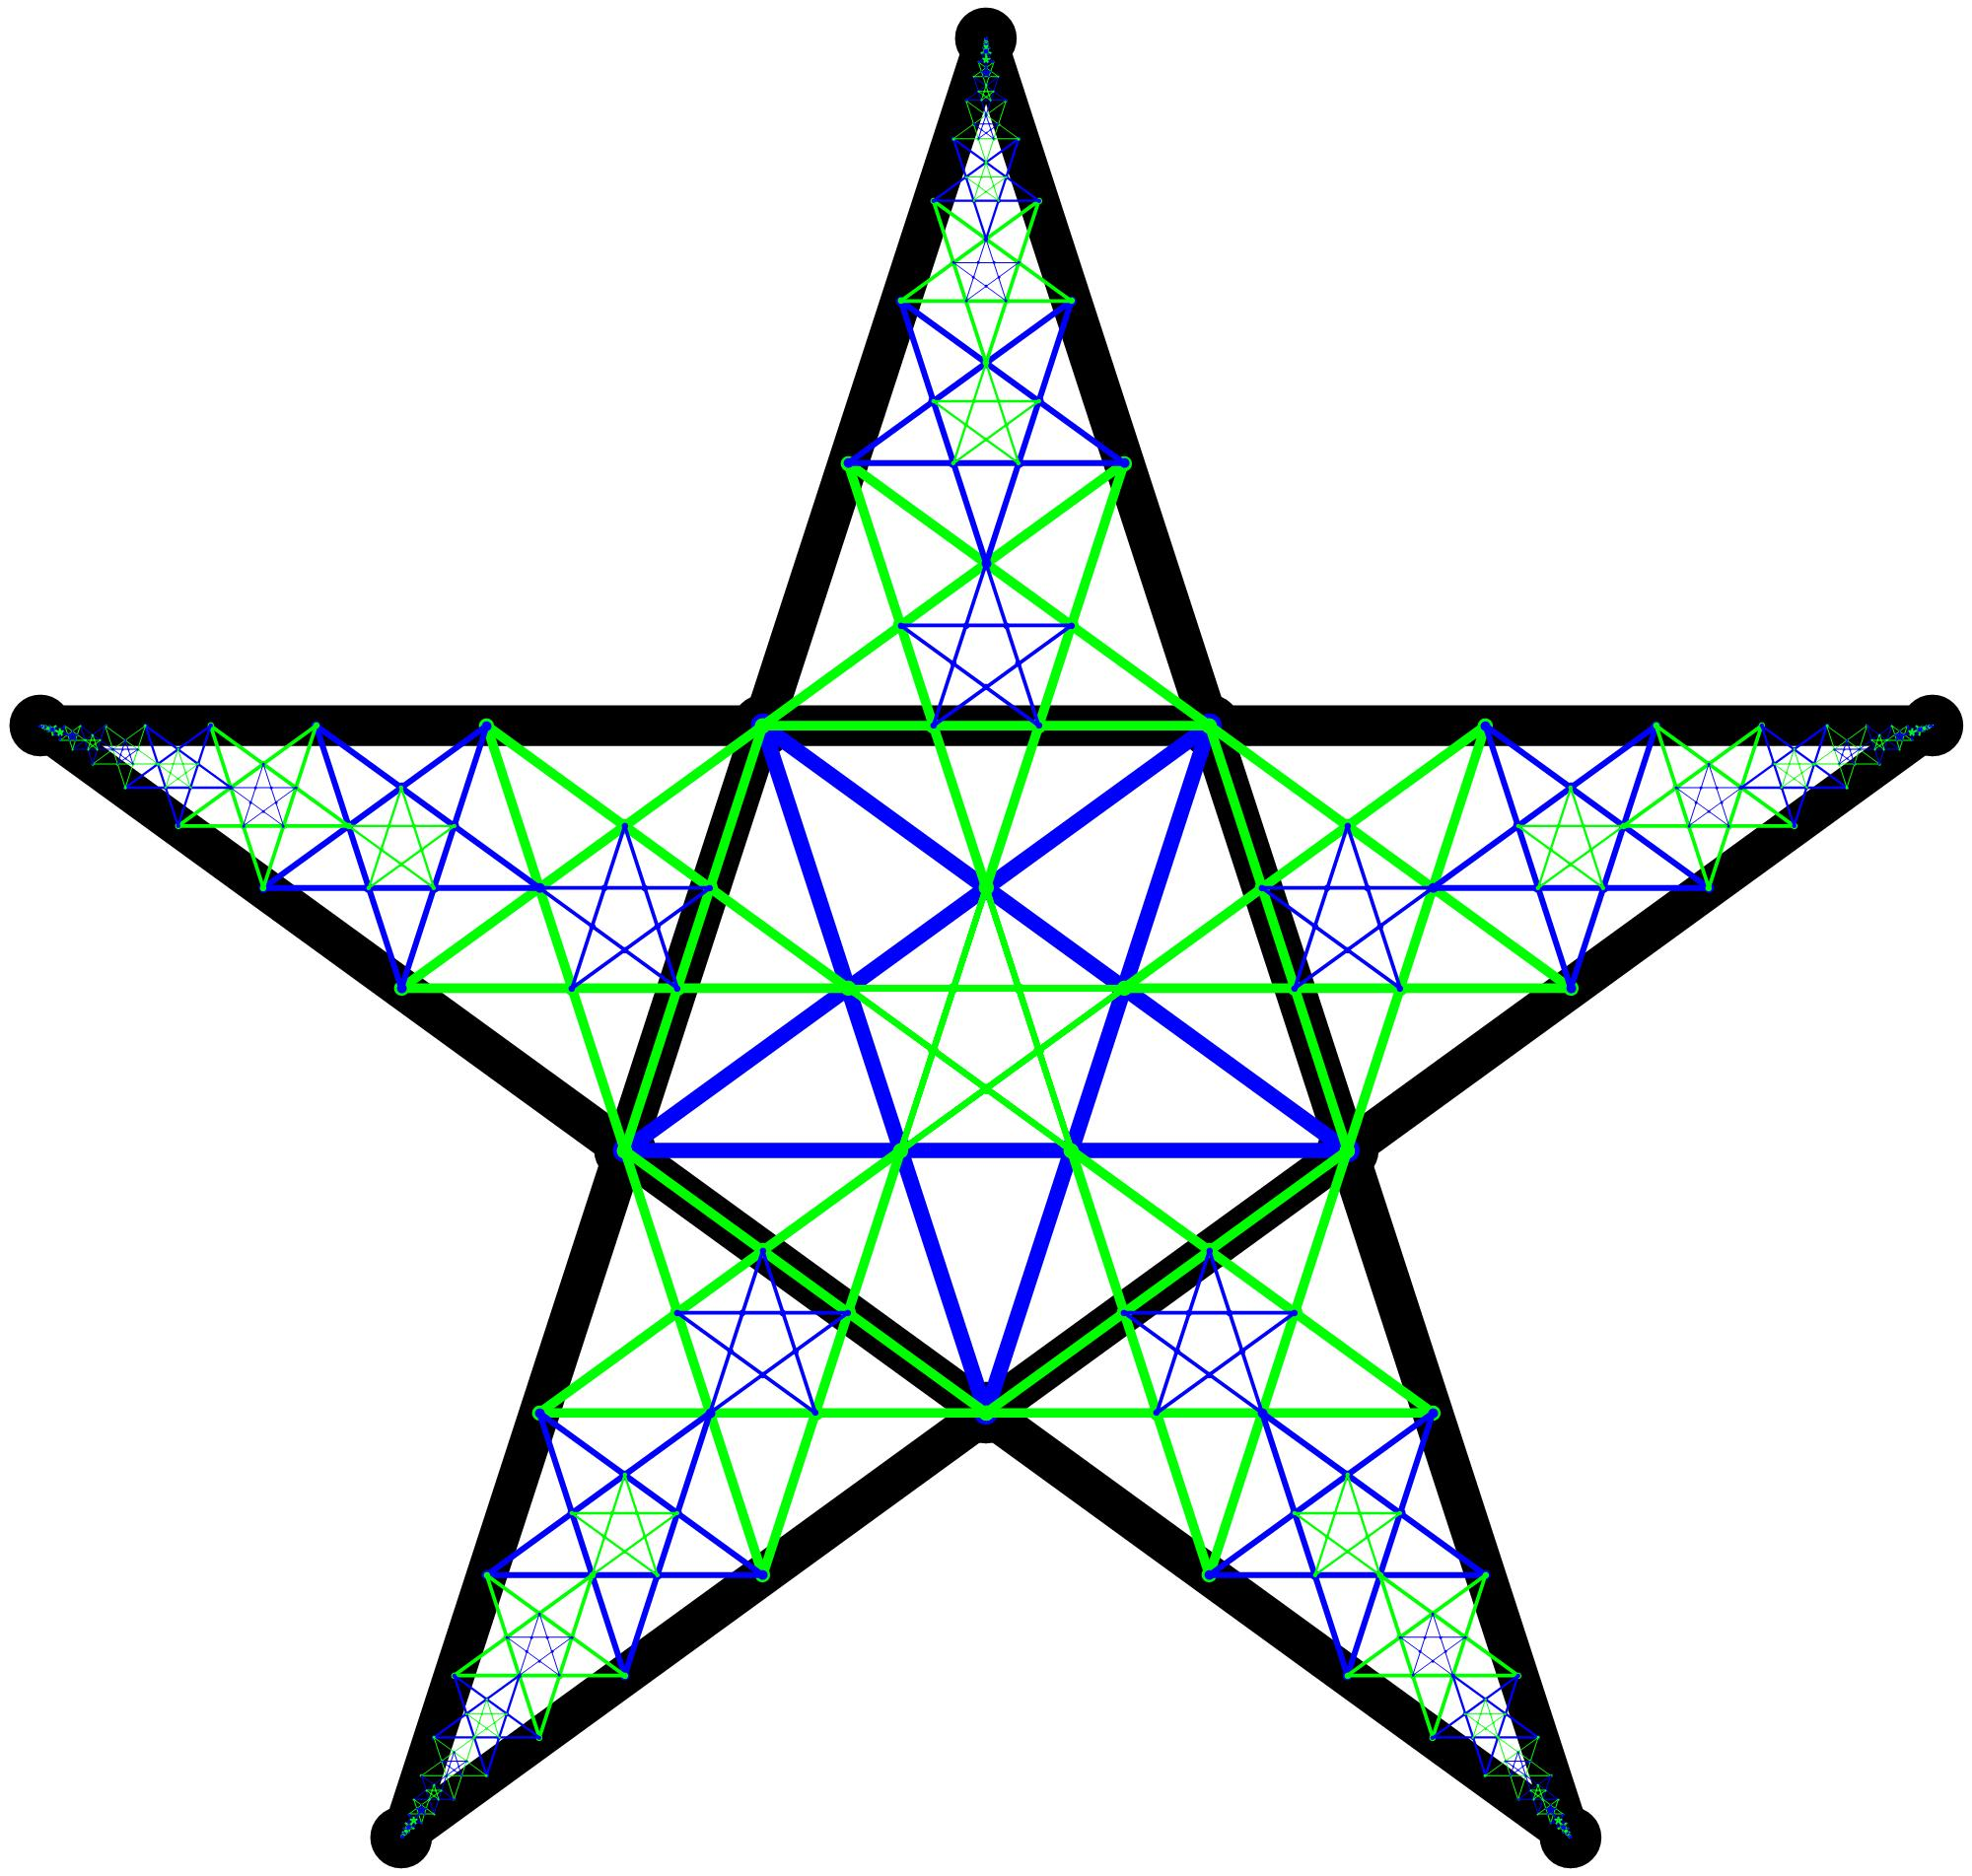
\includegraphics[max width=0.65\linewidth]{../images/pythagorean_pentagram.jpg}\]

\begin{enumerate}
\def\labelenumi{\arabic{enumi})}
\setcounter{enumi}{13}
\tightlist
\item
  James Dolan, ``Pythagorean pentagram'',
  \texttt{http://math.ucr.edu/home/baez/pythagorean\_pentagram.jpg}
\end{enumerate}

This is just the beginning of an infinite picture packed with
pentagrams. The sizes of these pentagrams are related by various powers
of the golden ratio: \[\Phi = \frac{1 + \sqrt5}{2} = 1.6180339\ldots\]
In particular, if you run up any arm of the big pentagram you'll see
little pentagrams, alternating blue and green in the above picture, each
\(1/\Phi\) times as big as the one before.

And if you contemplate these, you can see that: \[\Phi = 1 + 1/\Phi\] I
could explain how, but I prefer to leave it as a fun little puzzle. If
you get stuck, I'll give you a clue later.

This might have interested the Pythagoreans, since it quickly implies
that
\[\Phi = 1 + \frac1\Phi = 1 + \frac{1}{1 + \frac1\Phi} = 1 + \frac{1}{1 + \frac{1}{1 + \frac1\Phi}}\]
and so on. This means that the continued fraction expansion of \(\Phi\)
never ends, so it must be irrational! There's some evidence that early
Greeks were interested in continued fraction expansions\ldots{} you can
read about that in this marvelous speculative book:

\begin{enumerate}
\def\labelenumi{\arabic{enumi})}
\setcounter{enumi}{14}
\tightlist
\item
  David Fowler, \emph{The Mathematics Of Plato's Academy: A New
  Reconstruction}, 2nd edition, Clarendon Press, Oxford, 1999. Review by
  Fernando Q. Gouvêa for MAA Online available at
  \texttt{https://www.maa.org/press/maa-reviews/the-mathematics-of-platos-academy-a-new-reconstruction}
\end{enumerate}

If so, we can imagine that early Greek mathematicians discovered the
irrationality of the golden ratio by contemplating the Pythagorean
pentagram.

I recently gave a talk about this and other fun aspects of the number 5
at George Washington University and Google.

I was invited to Google by my student Mike Stay --- more about that some
other day, perhaps. But I'd been invited to George Washington University
by Bill Schmitt. We went to grad school together. While I was studying
quantum field theory with Irving Segal, he was studying combinatorics
with Gian-Carlo Rota. Later he taught me about Joyal's ``especes de
structures'', also known as ``species'' or ``structure types''. Later
still, these turned out to be deeply related to the quantum harmonic
oscillator and Feynman diagrams! For more on that, see
\protect\hyperlink{week185}{``Week 185''} and
\protect\hyperlink{week202}{``Week 202''}.

Bill has always been interested in getting Hopf algebras from structure
types. The idea is implicit in some work of Rota:

\begin{enumerate}
\def\labelenumi{\arabic{enumi})}
\setcounter{enumi}{15}
\item
  Saj-Nicole Joni and Gian-Carlo Rota, ``Coalgebras and bialgebras in
  combinatorics'', \emph{Studies in Applied Mathematics} \textbf{61}
  (1979), 93--139.

  Gian-Carlo Rota, ``Hopf algebras in combinatorics'', in
  \emph{Gian-Carlo Rota on Combinatorics: Introductory Papers and
  Commentaries}, ed.~J. P. S. Kung, Birkhauser, Boston, 1995.
\end{enumerate}

but my favorite explanation is here:

\begin{enumerate}
\def\labelenumi{\arabic{enumi})}
\setcounter{enumi}{16}
\tightlist
\item
  William R. Schmitt, ``Hopf algebras of combinatorial structures'',
  \emph{Canadian Journal of Mathematics} \textbf{45} (1993), 412--428.
  Also available at
  \texttt{http://home.gwu.edu/\textasciitilde{}wschmitt/papers/hacs.pdf}
\end{enumerate}

Let me sketch the simplest result in this paper! For starters, recall
that a structure type is any sort of structure you can put on finite
sets. In other words, it's a functor
\[F\colon \mathsf{FinSet}_0 \to \mathsf{Set}\] where
\(\mathsf{FinSet}_0\) is the groupoid of finite sets and bijections. The
idea is that for any finite set \(X\), \(F(X)\) is the set all of
structures of the given type that we can put on \(X\). A good example is
\(F(X) = 2^X\), the set of \(2\)-colorings of \(X\).

Starting from this, we can form a groupoid of \(F\)-structured finite
sets and structure-preserving bijections. For example, the groupoid of
\(2\)-colored finite sets and color-preserving bijections. The idea
should be obvious, but it's good to make it precise. For category
hotshots it's just the groupoid of ``elements'' of \(F\), called
\(\mathsf{elt}(F)\). But if you're not a hotshot yet, I should explain
this.

An object of \(\mathsf{elt}(F)\) is a finite set \(X\) together with an
element \(a\) in \(F(X)\). A morphism of \(\mathsf{elt}(F)\), say
\[f\colon (X,a) \to (X',a')\] is a bijection \[f\colon X \to X'\] such
that \[F(f)(a) = a'\] In other words: \(f\) is a bijection that carries
the \(F\)-structure on \(X\) to the \(F\)-structure on \(X'\).

Anyway: given a structure type \(F\), we can form a vector space \(B_F\)
whose basis consists of isomorphism classes of \(\mathsf{elt}(F)\). And
in the paper above, Bill describes various ways to make \(B_F\) into
various kinds of coalgebra or Hopf algebra.

I'll only explain the simplest one. There are lots of structure types
where you can ``restrict'' a structure on a big set to a structure on a
smaller set. For example, a \(2\)-coloring of a set restricts to a
\(2\)-coloring of any subset. Let's call such a thing a ``structure type
with restriction''.

Technically, a structure type with restriction is a functor
\[F\colon \mathsf{Inj}^\mathrm{op} \to \mathsf{Set}\] where
\(\mathsf{Inj}\) is the category of finite sets and injections. When we
have such a thing, the inclusion \[i\colon X \to X'\] of a little set
\(X\) in a bigger set \(X'\) gives a map \[F(i)\colon F(X') \to F(X)\]
that says how to restrict \(F\)-structures on \(X'\) to \(F\)-structures
on \(X\).

In this situation, Bill shows that the vector space \(B_F\) becomes a
cocommutative coalgebra. In particular, it gets a comultiplication
\[\Delta\colon B_F \to B_F \otimes B_F\] which satisfies laws just like
the commutative and associative laws for ordinary multiplication, only
``backwards''.

The idea is simple: we comultiply a finite set with an \(F\)-structure
on it by chopping the set in two parts in all possible ways and using
our ability to restrict the \(F\)-structure to each part. I could write
down the formula, but it's better to guess it and then check your guess
in Bill's paper! See his Proposition 3.1.

After Bill came up with this stuff, the connection between Hopf algebras
and combinatorics became a big business --- largely due to Kreimer's
work on Hopf algebras and Feynman diagrams. I talked about this back in
\protect\hyperlink{week122}{``Week 122''} --- but here's a more recent
review, with a hundred references for further study:

\begin{enumerate}
\def\labelenumi{\arabic{enumi})}
\setcounter{enumi}{17}
\tightlist
\item
  Kurusch Ebrahimi-Fard and Dirk Kreimer, ``Hopf algebra approach to
  Feynman diagram calculations'', available as
  \href{http://arXiv.org/abs/hep-th/0510202}{\texttt{hep-th/0510202}}.
\end{enumerate}

This yields lots of applications of Bill's ideas to quantum physics. I
have no idea how this huge industry is related to my work with James
Dolan and Jeffrey Morton on structure types, more general ``stuff
types'', quantum field theory and Feynman diagrams. But, maybe you can
figure it out if you read these:

\begin{enumerate}
\def\labelenumi{\arabic{enumi})}
\setcounter{enumi}{18}
\item
  John Baez and Derek Wise, \emph{Quantization and Categorification}.\\
  Fall 2003 notes: \texttt{http://math.ucr.edu/home/baez/qg-fall2003}\\
  Winter 2004 notes:
  \texttt{http://math.ucr.edu/home/baez/qg-winter2004/}\\
  Spring 2004 notes:
  \texttt{http://math.ucr.edu/home/baez/qg-spring2004/}
\item
  Jeffrey Morton, ``Categorified algebra and quantum mechanics'',
  \emph{Theory and Applications of Categories} \textbf{16} (2006),
  785--854. Available at
  \texttt{http://www.emis.de/journals/TAC/volumes/16/29/16-29abs.html}
  and as
  \href{http://arxiv.org/abs/math/0601458}{\texttt{math/0601458}}.
\end{enumerate}

While you're mulling over these ideas, it might pay to ponder this paper
Bill told me about:

\begin{enumerate}
\def\labelenumi{\arabic{enumi})}
\setcounter{enumi}{20}
\tightlist
\item
  Marcelo Aguiar and Swapneel Mahajan, ``Monoidal functors, species and
  Hopf algebras'', available at
  \texttt{http://www.math.tamu.edu/\textasciitilde{}maguiar/a.pdf}
\end{enumerate}

It's 588 pages long! It's a bunch of very sophisticated combinatorics
touching on ideas dear to my heart: \(q\)-deformation, species, Fock
space, and higher categories. I can't summarize it, but here are some
immediately gripping portions:

\begin{itemize}
\item
  Chapter 5, ``Higher monoidal categories''. Here they discuss
  ``\(n\)-monoidal categories'', which are categories equipped with a
  list of tensor products with lax interchange laws relating each tensor
  product to all the later ones on the list:
  \[(A \otimes_i B) \otimes_j (A' \otimes_i B') \to (A \otimes_j A') \otimes_i (B \otimes_j B')\]
  for \(i < j\). These gadgets generalize the ``iterated monoidal
  categories'' of Balteanu, Fiedorowicz, Schwaenzel, Vogt and also
  Forcey --- I gave some references on these back in
  \protect\hyperlink{week209}{``Week 209''}. The big difference seems to
  be that the Fiederowicz gang has all the tensor products share the
  same unit. That's great for what they want to do --- namely, get a
  kind of category whose nerve is an \(n\)-fold loop space. But, Aguiar
  and Mahajan study a bunch of examples coming from combinatorics where
  different products have different units! It's really these examples
  that are interesting to me, though the abstract concepts are cool too.
\item
  Chapter 7, ``Hopf monoids in species''. Here they use ``species'' to
  mean what I'd call ``linear structure types'', that is, functors
  \[F\colon \mathsf{FinSet}_0 \to \mathsf{Vect}\] where
  \(\mathsf{Vect}\) is the category of vector spaces. In Section 7.9
  they take Bill Schmitt's trick for getting cocommutative coalgebras
  from structure types with restriction, and use it to get
  cococommutative comonoids in the category of linear structure types!
  In Section 7.10 they take another trick to get coalgebras from
  structure types:

  \begin{enumerate}
  \def\labelenumi{\arabic{enumi})}
  \setcounter{enumi}{21}
  \tightlist
  \item
    William R. Schmitt, ``Incidence Hopf algebras'', \emph{Journal of
    Pure and Applied Algebra} \textbf{96} (1994), 299--330. Also
    available at
    \texttt{http://home.gwu.edu/\textasciitilde{}wschmitt/papers/iha.pdf}
  \end{enumerate}

  and do something similar with that.
\item
  Chapter 9, ``From species to graded vector spaces: Fock functors''.
  This studies what happens when you turn a Hopf monoid in the category
  of linear structure types into a graded Hopf algebra --- a kind of
  generalized Fock space.
\item
  Chapter 11, ``Hopf monoids from geometry''. Here they get Hopf monoids
  from the \(\mathrm{A}_n\) Coxeter complexes, using a lot of ideas
  related to Jacques Tits' theory of buildings. There's a lot of
  \(q\)-deformation going on here! All these ideas are close to my
  heart.
\end{itemize}

You can get more of a sense of what Aguiar is up to by looking at his
homepage. I'll just list a \emph{few} of the cool papers there:

\begin{enumerate}
\def\labelenumi{\arabic{enumi})}
\setcounter{enumi}{22}
\item
  Marcelo Aguiar's homepage,
  \texttt{http://www.math.tamu.edu/\textasciitilde{}maguiar/}

  Marcelo Aguiar, \emph{Internal categories and quantum groups},
  Ph.D.~thesis, Cornell University, August 1997. Available at
  \texttt{http://www.math.tamu.edu/\textasciitilde{}maguiar/thesis2.pdf}

  Marcelo Aguiar, ``Braids, \(q\)-binomials and quantum groups'',
  \emph{Advances in Applied Mathematics} \textbf{20} (1998) 323--365.
  Also available at
  \texttt{http://www.math.tamu.edu/\textasciitilde{}maguiar/braids.ps.gz}

  Marcelo Aguiar and Swapneel Mahajan, \emph{Coxeter groups and Hopf
  algebras}, Fields Institute Monographs, Volume \textbf{23}, AMS,
  Providence, RI, 2006. Also available at
  \texttt{http://www.math.tamu.edu/\textasciitilde{}maguiar/monograph.pdf}
\end{enumerate}

Check out the mysterious table of ``generalized binomial coefficients''
in the second of these papers --- it suggests many links between
different subjects of mathematics!

I was going to say a bit about quaternionic analysis, but now I'm worn
out. So, I'll just say that anyone interested in generalizing complex
analysis to the quaternions must read two papers. The first I had
managed to lose for a long time\ldots{} but now I've found it again:

\begin{enumerate}
\def\labelenumi{\arabic{enumi})}
\setcounter{enumi}{23}
\tightlist
\item
  Anthony Sudbery, ``Quaternionic analysis'', \emph{Math. Proc. Camb.
  Phil. Soc.} \textbf{85} (1979), 199--225. Available at
  \texttt{http://citeseer.ist.psu.edu/10590.html} and (slightly
  different version)
  \texttt{http://theworld.com/\textasciitilde{}sweetser/quaternions/ps/Quaternionic-analysis.pdf}
\end{enumerate}

The second was brought to my attention by David Corfield:

\begin{enumerate}
\def\labelenumi{\arabic{enumi})}
\setcounter{enumi}{24}
\tightlist
\item
  Igor Frenkel and Matvei Libine, ``Quaternionic analysis,
  representation theory and physics'', available as
  \href{http://arxiv.org/abs/0711.2699}{\texttt{arXiv:0711.2699}}
\end{enumerate}

Since Igor Frenkel is a bigshot, this paper may finally bring this
neglected subject some of the attention it deserves! Like Corfield, I'll
just quote the abstract, to make your mouth water:

\begin{quote}
We develop quaternionic analysis using as a guiding principle
representation theory of various real forms of the conformal group. We
first review the Cauchy-Fueter and Poisson formulas and explain their
representation theoretic meaning. The requirement of unitarity of
representations leads us to the extensions of these formulas in
Minkowski space, which can be viewed as another real form of
quaternions. Representation theory also suggests a quaternionic version
of the Cauchy formula for the second order pole. Remarkably, the
derivative appearing in the complex case is replaced by the Maxwell
equations in the quaternionic counterpart. We also uncover the
connection between quaternionic analysis and various structures in
quantum mechanics and quantum field theory, such as the spectrum of the
hydrogen atom, polarization of vacuum, and one-loop Feynman integrals.
We also make some further conjectures. The main goal of this and our
subsequent paper is to revive quaternionic analysis and to show profound
relations between quaternionic analysis, representation theory and
four-dimensional physics.
\end{quote}

Finally, here's a clue for the Pythagorean pentagram puzzle. To prove
that \[\Phi = 1 + 1/\Phi,\] show the length of the longest red interval
here is the sum of the lengths of the two shorter ones:
\[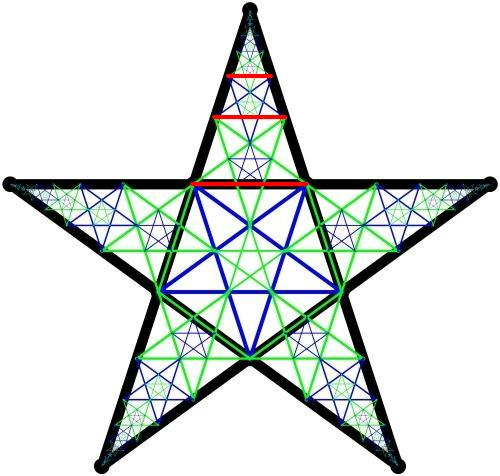
\includegraphics[max width=0.65\linewidth]{../images/golden_ratio_pentagram.jpg}\]

\begin{enumerate}
\def\labelenumi{\arabic{enumi})}
\setcounter{enumi}{25}
\tightlist
\item
  James Dolan and John Baez, ``annotated picture of Pythagorean
  pentagram'',
  \texttt{http://math.ucr.edu/home/baez/golden\_ratio\_pentagram.jpg}
\end{enumerate}

For more on the golden ratio, try \protect\hyperlink{week203}{``Week
203''}. For more on its relation to the dodecahedron, see
\protect\hyperlink{week241}{``Week 241''}.

\begin{center}\rule{0.5\linewidth}{0.5pt}\end{center}

\textbf{Addenda:} Here's another stunning picture of the ridges and
cracks on Europa:
\[\href{http://photojournal.jpl.nasa.gov/catalog/PIA03002}{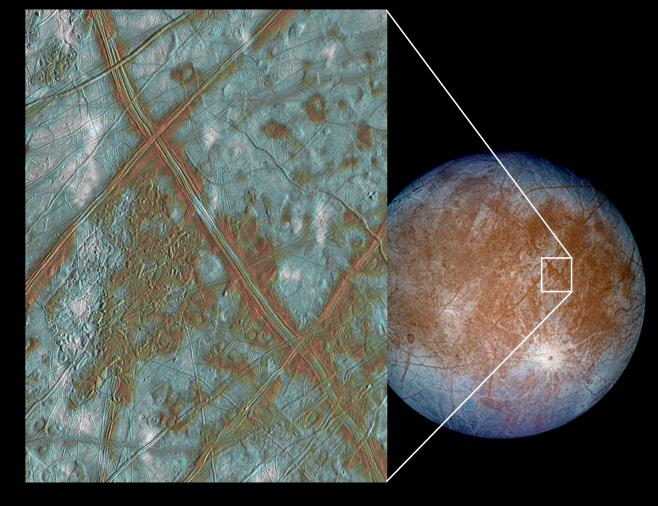
\includegraphics[max width=0.65\linewidth]{../images/europa_ice_cracks.jpg}}\]

\begin{enumerate}
\def\labelenumi{\arabic{enumi})}
\setcounter{enumi}{26}
\tightlist
\item
  NASA Photojournal, ``Blocks in the Europan crust provide more evidence
  of subterranean ocean'',
  \texttt{http://photojournal.jpl.nasa.gov/catalog/PIA03002}
\end{enumerate}

You can see more discussion of this Week's Finds at the
\href{http://golem.ph.utexas.edu/category/2008/05/this_weeks_finds_in_mathematic_26.html}{\(n\)-Category
Café}. You can also see a list of questions I'd like your help with!

\begin{center}\rule{0.5\linewidth}{0.5pt}\end{center}

\begin{quote}
\emph{There is geometry in the humming of the strings, there is music in
the spacing of the spheres.} --- Pythagoras
\end{quote}



\hypertarget{week266}{%
\section{June 20, 2008}\label{week266}}

I'm at this workshop now, and I want to talk about it:

\begin{enumerate}
\def\labelenumi{\arabic{enumi})}
\tightlist
\item
  \emph{Workshop on Categorical Groups}, June 16--20, 2008, Universitat
  de Barcelona, organized by Pilar Carrasco, Josep Elgueta, Joachim Kock
  and Antonio Rodríguez Garzón,
  \texttt{http://mat.uab.cat/\textasciitilde{}kock/crm/hocat/cat-groups/}
\end{enumerate}

But first, the moon of the week --- and a bit about that mysterious
fellow Pythagoras, and the Pythagorean tuning system.

Here's a picture of Jupiter's moon Io:
\[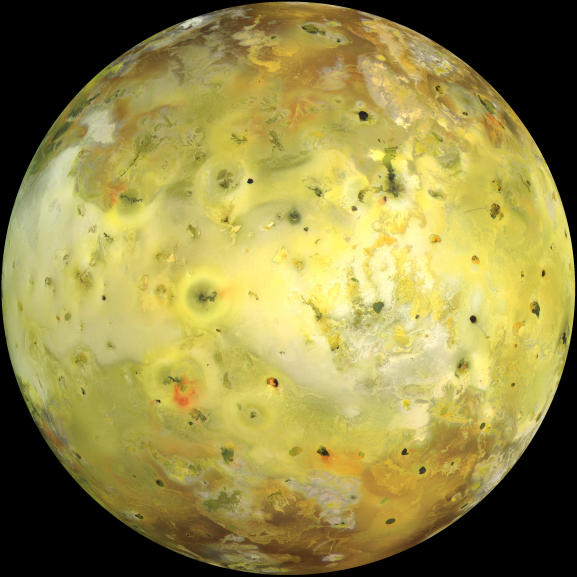
\includegraphics[max width=0.65\linewidth]{../images/io.jpg}\]

\begin{enumerate}
\def\labelenumi{\arabic{enumi})}
\tightlist
\item
  ``Io in True Color'', Astronomy Picture of the Day,
  \texttt{http://antwrp.gsfc.nasa.gov/apod/ap040502.html}
\end{enumerate}

It's yellow! --- a world covered with sulfur spewed from volcanos,
burning hot inside from intense tidal interactions with Jupiter's mighty
gravitational field\ldots{} but frigid at the surface.

Last week I talked about something called the ``Pythagorean pentagram''.
That's a cool name --- but it's far from clear who first discovered this
entity, so I started feeling a bit guilty for using it, and I started
wondering what we actually know about Pythagoras or the mathematical
vegetarian cult he supposedly launched. Tim Silverman pointed me to a
scholarly book on the subject:

\begin{enumerate}
\def\labelenumi{\arabic{enumi})}
\setcounter{enumi}{1}
\tightlist
\item
  Walter Burkert, \emph{Lore and Science in Ancient Pythagoreanism},
  Harvard U. Press, Cambridge, Massachusetts, 1972.
\end{enumerate}

It turns out we know very little about Pythagoras: a few grains of solid
fact, surrounded by a huge cloud of stories that grows larger and larger
as we move further and further away from the 6th century BC, when he
lived. This is especially true when it comes to his contributions to
mathematics. The infamous pseudohistorian Eric Temple Bell begins his
book ``The Magic of Numbers'' as follows:

\begin{quote}
The hero of our story is Pythagoras. Born to immortality five hundred
years before the Christian era began, this titanic spirit overshadows
western civilization. In some respects he is more vividly alive today
than he was in his mortal prime twenty-five centuries ago, when he
deflected the momentum of prescientific history toward our own
unimagined scientific and technological culture. Mystic, philosopher,
experimental physicist, and mathematician of the first rank, Pythagoras
dominated the thought of his age and foreshadowed the scientifi
mysticisms of our own.
\end{quote}

But, there's no solid evidence for any of this, except perhaps his
interest in mysticism and numerology and the incredible growth of his
legend as the centuries pass. We're not even sure he proved the
``Pythagorean theorem'', much less all the other feats that have been
attributed to him. As Burkert explains:

\begin{quote}
No other branch of history offers such temptations to conjectural
reconstruction as does the history of mathematics. In mathematics, every
detail has its fixed and unalterable place in a nexus of relations, so
that it is often possible, on the basis of a brief and casual remark, to
reconstruct a complicated theory. It is not surprising, then, that gap
in the history of mathematics that was opened up by a critical study of
the evidence about Pythagoras has been filled by a whole succession of
conjectural supplements.
\end{quote}

There's a new book out on Pythagoras:

\begin{enumerate}
\def\labelenumi{\arabic{enumi})}
\setcounter{enumi}{2}
\tightlist
\item
  Kitty Ferguson, \emph{The Music of Pythagoras: How an Ancient
  Brotherhood Cracked the Code of the Universe and Lit the Path from
  Antiquity to Outer Space}, Walker and Company, 2008.
\end{enumerate}

The subtitle is sensationalistic, exactly the sort of thing that would
make Burkert cringe. But the book is pretty good, and Ferguson is honest
about this: after asking ``What do we know about Pythagoras?'', she
lists everything we know in one short paragraph, and then emphasizes:
that's \emph{all}.

He was born on the island of Samos sometime around 575 BC. He went to
Croton, a city in what is now southern Italy. He died around 495 BC. We
know a bit more --- but not much.

It's much easier to learn about the Renaissance ``neo-Pythagoreans''.
This book is a lot of fun, though too romantic to be truly scholarly:

\begin{enumerate}
\def\labelenumi{\arabic{enumi})}
\setcounter{enumi}{3}
\tightlist
\item
  S. K. Heninger, Jr., \emph{Touches of Sweet Harmony: Pythagorean
  Cosmology and Renaissance Poetics}, The Huntington Library, San
  Marino, California, 1974.
\end{enumerate}

It seems clear that the Renaissance neo-Pythagoreans, and even the Greek
Pythagoreans, and perhaps even old Pythagoras himself were much taken
with something called the tetractys: \[
  \begin{tikzpicture}[xscale=0.7,yscale=0.6]
    \node at (0,0) {$\bullet$};
    \node at (1,0) {$\bullet$};
    \node at (2,0) {$\bullet$};
    \node at (3,0) {$\bullet$};
    \node at (0.5,1) {$\bullet$};
    \node at (1.5,1) {$\bullet$};
    \node at (2.5,1) {$\bullet$};
    \node at (1,2) {$\bullet$};
    \node at (2,2) {$\bullet$};
    \node at (1.5,3) {$\bullet$};
  \end{tikzpicture}
\] To appreciate the tetractys, you have to temporarily throw out modern
scientific thinking and get yourself in the mood of magical thinking ---
or ``correlative cosmology'', which tries to understand the universe by
setting up elaborate correspondences between this, that, and the other
thing. To the Pythagoreans, the four rows of the tetractys represented
the point, line, triangle and tetrahedron. But the ``fourness'' of the
tetractys also represented the four classical elements: earth, air,
water and fire. It's fun to compare these early groping attempts to
impose order on the universe to later, less intuitive but far more
predictively powerful schemes like the Periodic Table or the Standard
Model. So, let's take a look!

The Renaissance thinkers liked to organize the four elements using a
chain of analogies running from light to heavy:

\begin{quote}
fire : air :: air : water :: water : earth
\end{quote}

Them also organized them in a diamond, like this: \[
  \begin{tikzpicture}[scale=0.7]
    \node at (0:2) {\textbf{earth}};
    \node at (45:2) {dry};
    \node at (90:2) {\textbf{fire}};
    \node at (135:2) {hot};
    \node at (180:2) {\textbf{air}};
    \node at (225:2) {wet};
    \node at (270:2) {\textbf{water}};
    \node at (315:2) {cold};
  \end{tikzpicture}
\] Sometimes they even put a fifth element in the middle: the
``quintessence'', or ``aether'', from which heavenly bodies were made.
And following Plato's Timaeus dialog, they set up an analogy like this:

\begin{longtable}[]{@{}ll@{}}
\toprule
\endhead
fire & tetrahedron\tabularnewline
air & octahedron\tabularnewline
water & icosahedron\tabularnewline
earth & cube\tabularnewline
quintessence & dodecahedron\tabularnewline
\bottomrule
\end{longtable}

This is cute! Fire feels pointy and sharp like tetrahedra, while water
rolls like round icosahedra, and earth packs solidly like cubes.
Dodecahedra are different than all the rest, made of pentagons, just as
you might expect of ``quintessence''. And air\ldots{} well, I've never
figured out what air has to do with octahedra. You win some, you lose
some --- and in correlative cosmology, a discrepancy here and there
doesn't falsify your ideas.

The tetractys also took the Pythagoreans in other strange directions.
For example, who said this?

\begin{quote}
``What you suppose is four is really ten\ldots{}''
\end{quote}

A modern-day string theorist talking to Lee Smolin about the dimension
of spacetime? No! Around 150 AD, the rhetorician Lucian of Samosata
attributed this quote to Pythagoras, referring to the tetratkys and the
fact that it has \(1 + 2 + 3 + 4 = 10\) dots. This somehow led the
Pythagoreans to think the number 10 represented ``perfection''. If there
turn out to be 4 visible dimensions of spacetime together with 6
curled-up ones explaining the gauge group
\(\mathrm{U}(1) \times \mathrm{SU}(2) \times \mathrm{SU}(3)\), maybe
they were right.

Pythagorean music theory is a bit more comprehensible: along with
astronomy, music is one of the first places where mathematical physics
made serious progress. The Greeks, and the Babylonians before them, knew
that nice-sounding intervals in music correspond to simple rational
numbers. For example, they knew that the octave corresponds to a ratio
of \(2:1\). We'd now call this a ratio of \emph{frequencies}; one can
get into some interesting scholarly arguments about when and how well
the Greeks knew that sound was a \emph{vibration}, but never mind ---
read Burkert's book if you're interested.

Whatever these ratios meant, the Greeks also knew that a fifth
corresponds to a ratio of \(3:2\), and a fourth to \(4:3\).

By the way, if you don't know about musical intervals like ``fourths''
and ``fifths'', don't feel bad. I won't explain them now, but you can
learn about them and hear them here:

\begin{enumerate}
\def\labelenumi{\arabic{enumi})}
\setcounter{enumi}{4}
\tightlist
\item
  Brian Capleton, ``Musical intervals'',
  \texttt{http://www.amarilli.co.uk/music/intervs.htm}
\end{enumerate}

and then practice recognizing them:

\begin{enumerate}
\def\labelenumi{\arabic{enumi})}
\setcounter{enumi}{5}
\tightlist
\item
  Ricci Adams, ``Interval ear trainer'',
  \texttt{http://www.musictheory.net/trainers/html/id90\_en.html}
\end{enumerate}

If you nose around Capleton's website, you'll see he's quite a
Pythagorean mystic himself!

Anyway, at some moment, lost in history by now, people figured out that
the octave could be divided into a fourth and a fifth:
\[\frac21 = \frac43 \times \frac32\] And later, I suppose, they defined
a whole tone to be the difference, or really ratio, between a fifth and
a fourth: \[\frac{3/2}{4/3} = \frac98\] So, when you go up one whole
tone in the Pythagorean tuning system, the higher note should vibrate
\(9/8\) as fast as the lower one. If you try this on a modern keyboard,
it looks like after going up 6 whole tones you've gone up an octave. But
in fact if you buy the Pythagorean definition of whole tone, 6 whole
tones equals
\[(\frac98)^6 = \frac{531441}{262144} \approx 2.027286530\ldots\] which
is, umm, not quite 2!

Another way to put it is that if you go up 12 fifths, you've
\emph{almost} gone up 7 octaves, but not quite: the so-called circle of
fifths doesn't quite close, since
\[\frac{(3/2)^{12}}{2^7} = \frac{531441}{524288} \approx 1.01264326\ldots\]
This annoying little discrepancy is called the ``Pythagorean comma''.

This sort of discrepancy is an unavoidable fact of mathematics. Our ear
likes to hear frequency ratios that are nice simple rational numbers,
and we'd also like a scale where the notes are evenly spaced --- but we
can't have both. Why? Because you can't divide an octave into equal
parts that are rational ratios of frequencies. Why? Because a nontrivial
\(n\)th root of 2 can never be rational.

So, irrational numbers are lurking in any attempt to create an equally
spaced (or as they say, ``equal-tempered'') tuning system.

You might imagine this pushed the Pythagoreans to confront irrational
numbers. This case has been made by the classicist Tannery, but Burkert
doesn't believe it: there's no written evidence suggesting it.

You could say the existence of irrational numbers is the root of all
evil in music. Indeed, the diminished fifth in an equal tempered scale
is called the ``diabolus in musica'', or ``devil in music'', and it has
a frequency ratio equal to the square root of 2.

Or, you could say that this built-in conflict is the spice of life! It
makes it impossible for harmony to be perfect and therefore dull.

Anyway, Pythagorean tuning is not equal-tempered: it's based on making
lots of fifths equal to exactly \(3/2\). So, all the frequency ratios
are fractions built from the numbers 2 and 3. But, some of them are
nicer than others:

\begin{itemize}
\tightlist
\item
  first = \(1/1\)
\item
  second = \(9/8\)
\item
  third = \(81/64\)
\item
  fourth = \(4/3\)
\item
  fifth = \(3/2\)
\item
  sixth = \(27/16\)
\item
  seventh = \(243/128\)
\item
  octave = \(2/1\)
\end{itemize}

As you can see, the third, sixth and seventh are not very nice: they're
complicated fractions, so they don't sound great. They're all a bit
sharp compared to the following tuning system, which is a form of ``just
intonation'':

\begin{itemize}
\tightlist
\item
  first = \(1/1\)
\item
  second = \(9/8\)
\item
  third = \(5/4\)
\item
  fourth = \(4/3\)
\item
  fifth = \(3/2\)
\item
  sixth = \(5/3\)
\item
  seventh = \(15/8\)
\item
  octave = \(2/1\)
\end{itemize}

Just intonation brings in fractions involving the number 5, which we
might call the ``quintessence'' of music: we need it to get a
nice-sounding third. A long and interesting tale could be told about
this tuning system --- but not now. Instead, let's just see how the
third, sixth and seventh differ:

\begin{itemize}
\tightlist
\item
  In just intonation the third is \(5/4 = 1.25\), but in Pythagorean
  tuning it's \(81/64 = 1.265625\). The Pythagorean system is about
  1.25\% sharp.
\item
  In just intonation the sixth is \(5/3 = 1.6666\ldots\), but in
  Pythagorean tuning it's \(81/64 = 1.6875\). The Pythagorean system is
  about 0.7\% sharp.
\item
  In just intonation the seventh is \(15/8 = 1.875\), but in Pythagorean
  tuning it's \(243/128 = 1.8984375\). The Pythagorean system is about
  1.25\% sharp.
\end{itemize}

Here you can learn more about Pythagorean tuning, and hear it in action:

\begin{enumerate}
\def\labelenumi{\arabic{enumi})}
\setcounter{enumi}{6}
\item
  Margo Schulter, ``Pythagorean tuning and medieval polyphony'',
  \texttt{http://www.medieval.org/emfaq/harmony/pyth.html}
\item
  Reginald Bain, ``A Pythagorean tuning of the diatonic scale'',
  \texttt{http://www.music.sc.edu/fs/bain/atmi02/pst/index.html}
\end{enumerate}

There's also a murky relation between Pythagorean tuning and something
called the ``Platonic Lambda''. This is a certain way of labelling the
edges of the tetractys by powers of \(2\) on one side, and powers of
\(3\) on the other: \[
  \begin{tikzpicture}[xscale=0.7,yscale=0.6]
    \node at (0,0) {$1$};
    \node at (-0.5,-1) {$2$};
    \node at (0.5,-1) {$3$};
    \node at (-1,-2) {$4$};
    \node at (1,-2) {$9$};
    \node at (-1.5,-3) {$8$};
    \node at (1.5,-3) {$27$};
  \end{tikzpicture}
\] I can't help wanting to flesh it out like this, so going down and to
the left is multiplication by \(2\), while going down and to the right
is multiplication by \(3\): \[
  \begin{tikzpicture}[xscale=0.7,yscale=0.6]
    \node at (0,0) {$1$};
    \node at (-0.5,-1) {$2$};
    \node at (0.5,-1) {$3$};
    \node at (-1,-2) {$4$};
    \node at (0,-2) {$6$};
    \node at (1,-2) {$9$};
    \node at (-1.5,-3) {$8$};
    \node at (-0.5,-3) {$12$};
    \node at (0.5,-3) {$18$};
    \node at (1.5,-3) {$27$};
  \end{tikzpicture}
\] So, I was pleased when in Heninger's book I saw the numbers on the
bottom row in a plate from a 1563 edition of ``De Natura Rerum'', a
commentary on Plato's Timaeus written by the Venerable Bede sometime
around 700 AD!

In this plate, the elements fire, air, water and earth are labelled by
the numbers 8, 12, 18 and 27. This makes the aforementioned analogies:

\begin{quote}
fire : air :: air : water :: water : earth
\end{quote}

into strict mathematical proportions:

\begin{quote}
8 : 12 :: 12 : 18 :: 18 : 27
\end{quote}

Cute! Of course it doesn't do much to help us understand fire, air,
earth and water. But, it goes to show how people have been struggling a
long time to find mathematical patterns in nature. Most of these
attempts don't work. Occasionally we get lucky\ldots{} and over the
millennia, these scraps of luck added up to the impressive theories we
have today.

Next: the categorical groups workshop here in Barcelona!

A ``categorical group'', also called a ``\(2\)-group'', is a category
that's been equipped with structures mimicking those of a group: a
product, identity, and inverses, satisfying the usual laws either
``strictly'' as equations or ``weakly'' as natural isomorphisms. Pretty
much anything people do with groups can also be done with \(2\)-groups.
That's a lot of stuff --- so there's a lot of scope for exploration!
There's a powerful group of algebraists in Spain engaged in this
exploration, so it makes sense to have this workshop here.

Let me say a little about some of the talks we've had so far. I'll
mainly give links, instead of explaining stuff in detail.

On Monday, I kicked off the proceedings with this talk:

\begin{enumerate}
\def\labelenumi{\arabic{enumi})}
\setcounter{enumi}{8}
\tightlist
\item
  John Baez, ``Classifying spaces for topological \(2\)-groups'',
  \texttt{http://math.ucr.edu/home/baez/barcelona/}
\end{enumerate}

Just as we can try to classify principal bundles over some space with
any fixed group as gauge group, we can try to classify ``principal
\(2\)-bundles'' with a given ``gauge \(2\)-group''. It's a famous old
theorem that for any topological group \(G\), we can find a space \(BG\)
such that principal \(G\)-bundles over any mildly nice space \(X\) are
classified by maps from \(X\) to \(BG\). (Homotopic maps correspond to
isomorphic bundles.) A similar result holds for topological
\(2\)-groups!

Indeed, Baas Bkstedt and Kro did something much more general for
topological \emph{\(2\)-categories}:

\begin{enumerate}
\def\labelenumi{\arabic{enumi})}
\setcounter{enumi}{9}
\tightlist
\item
  Nils Baas, Marcel Bkstedt and Tore Kro, ``\(2\)-Categorical
  K-theories'', available as
  \href{http://arXiv.org/abs/math/0612549}{\texttt{math/0612549}}.
\end{enumerate}

Just as a group is a category with one object and with all morphisms
being invertible, a \(2\)-group is a \(2\)-category with one object and
all morphisms and \(2\)-morphisms invertible. But the \(2\)-group case
is worthy of some special extra attention, so Danny Stevenson studied
that with a little help from me:

\begin{enumerate}
\def\labelenumi{\arabic{enumi})}
\setcounter{enumi}{10}
\tightlist
\item
  John Baez and Danny Stevenson, ``The classifying space of a
  topological \(2\)-group'', available as
  \href{http://arxiv.org/abs/0801.3843}{\texttt{arXiv/0801.3843}}
\end{enumerate}

and that's what I talked about. If you're also interested in classifying
spaces of \(2\)-categories that aren't topological, just ``discrete'',
you should try these:

\begin{enumerate}
\def\labelenumi{\arabic{enumi})}
\setcounter{enumi}{11}
\item
  John Duskin, ``Simplicial matrices and the nerves of weak
  \(n\)-categories I: nerves of bicategories'', available at
  \texttt{http://www.tac.mta.ca/tac/volumes/9/n10/9-10abs.html}
\item
  Manuel Bullejos and A. Cegarra, ``On the geometry of \(2\)-categories
  and their classifying spaces'', available at
  \texttt{http://www.ugr.es/\%7Ebullejos/geometryampl.pdf}
\item
  Manuel Bullejos, Emilio Faro and Victor Blanco, ``A full and faithful
  nerve for \(2\)-categories'', \emph{Applied Categorical Structures}
  \textbf{13} (2005), 223--233. Also available as
  \href{http://arXiv.org/abs/math/0406615}{\texttt{arXiv:math/0406615}}.
\end{enumerate}

On Monday afternoon, Bruce Bartlett spoke on a geometric way to
understand representations and ``\(2\)-representations'' of ordinary
finite groups. You can see his talk here, and also a version which has
less material, explained in a more elementary way:

\begin{enumerate}
\def\labelenumi{\arabic{enumi})}
\setcounter{enumi}{14}
\item
  Bruce Bartlett, ``The geometry of unitary \(2\)-representations of
  finite groups and their \(2\)-characters'', talk at the
  \emph{Categorical Groups workshop in Barcelona}, June 16, 2008,
  available at
  \texttt{http://brucebartlett.postgrad.shef.ac.uk/research/Barcelona.pdf}

  Bruce Bartlett, ``The geometry of \(2\)-representations of finite
  groups'', talk at the Max Kelly Conference, Cape Town, 2008, available
  at
  \texttt{http://brucebartlett.postgrad.shef.ac.uk/research/MaxKellyTalk.pdf}
\end{enumerate}

Both talks are based on this paper:

\begin{enumerate}
\def\labelenumi{\arabic{enumi})}
\setcounter{enumi}{15}
\tightlist
\item
  Bruce Bartlett, ``The geometry of unitary \(2\)-representations of
  finite groups and their \(2\)-characters'', draft available at
  \texttt{http://brucebartlett.postgrad.shef.ac.uk/research/Max\%20Kelly\%20Proceedings.pdf}
\end{enumerate}

The first big idea here is that the category of representations of a
finite group \(G\) is equivalent to some category where an object \(X\)
is a complex manifold on which \(G\) acts, equipped with an invariant
hermitian metric and an equivariant \(\mathrm{U}(1)\) bundle. A morphism
from \(X\) to \(Y\) in this category is not just the obvious sort of
map; instead, it's diagram of maps shaped like this: \[
  \begin{tikzcd}
    &S\drar["F"]\dlar[swap,"G"]&
  \\X&&Y
  \end{tikzcd}
\] This is called a ``span''. So, we're seeing a very nice extension of
the Tale of Groupoidification, which began in
\protect\hyperlink{week247}{``Week 247''} and continued up to
\protect\hyperlink{week257}{``Week 257''}, when it jumped over to my
seminar.

But Bruce doesn't stop here! He then \emph{categorifies} this whole
story, replacing representations of \(G\) on Hilbert spaces by
representations on \(2\)-Hilbert spaces, and replacing \(\mathrm{U}(1)\)
bundles by \(\mathrm{U}(1)\) gerbes. This is quite impressive, with nice
applications to a topological quantum field theory called the
Dijkgraaf-Witten model.

Next, to handle the TQFT called Chern-Simons theory, Bruce plans to
replace the finite group \(G\) by a compact Lie group. Another, stranger
direction he could go is to replace \(G\) by a finite \(2\)-group. Then
he'd make contact with the categorified Dijkgraaf-Witten TQFT studied in
these papers:

\begin{enumerate}
\def\labelenumi{\arabic{enumi})}
\setcounter{enumi}{16}
\item
  David Yetter, ``TQFT's from homotopy \(2\)-types'', \emph{Journal of
  Knot Theory and its Ramifications} \textbf{2} (1993), 113--123.
\item
  Timothy Porter and Vladimir Turaev, ``Formal homotopy quantum field
  theories, I: Formal maps and crossed C-algebras'', available as
  \href{http://arXiv.org/abs/math/0512032}{\texttt{arXiv:math/0512032}}.

  Timothy Porter and Vladimir Turaev, ``Formal homotopy quantum field
  theories, II: Simplicial formal maps'', in \emph{Categories in
  Algebra, Geometry and Mathematical Physics}, eds.~A. Davydov et al,
  Contemp. Math \textbf{431}, AMS, Providence Rhode Island, 2007,
  375--403. Also available as
  \href{http://arXiv.org/abs/math/0512034}{\texttt{arXiv:math/0512034}}.
\item
  Joo Faria Martins and Timothy Porter, ``On Yetter's invariant and an
  extension of the Dijkgraaf-Witten invariant to categorical groups'',
  available as
  \href{http://arXiv.org/abs/math/0608484}{\texttt{arXiv:math/0608484}}.
\end{enumerate}

As the last paper explains, we can also think of this TQFT as a field
theory where the ``field'' on a spacetime \(X\) is a map
\[f\colon X \to BG\] where \(BG\) is the classifying space of the
\(2\)-group \(G\).

Given all this, it's natural to contemplate a further generalization of
Bruce's work where \(G\) is a Lie \(2\)-group. Unfortunately, Lie
\(2\)-groups don't have many representations on \(2\)-Hilbert space of
the sort I've secretly been talking about so far: that is,
finite-dimensional ones.

So we may, perhaps, need to ponder representations of Lie \(2\)-groups
on infinite-dimensional \(2\)-Hilbert spaces.

Luckily, that's just what Derek Wise spoke about on Wednesday morning!
His talk also included some pictures with intriguing relations to the
pictures in Bruce's talk. You can see the slides here:

\begin{enumerate}
\def\labelenumi{\arabic{enumi})}
\setcounter{enumi}{18}
\tightlist
\item
  Derek Wise, ``Representations of \(2\)-groups on higher Hilbert
  spaces'',
  \texttt{http://math.ucdavis.edu/\textbackslash{}\textasciitilde{}derek/talks/barcelona2008.pdf}
\end{enumerate}

They make a nice introduction to a paper he's writing with Aristide
Baratin, Laurent Freidel and myself. Our work uses ideas like measurable
fields of Hilbert spaces, which are already important for understanding
infinite-dimensional unitary group representations. But if you're less
fond of analysis, jump straight to pages 20, 23 and 25, where he gives a
geometrical interpretation of these infinite-dimensional
representations, along with the intertwining operators between
them\ldots{} and the ``\(2\)-intertwining operators'' between
\emph{those}.

This work relies heavily on the work of Crane, Sheppeard and Yetter,
cited in \protect\hyperlink{week210}{``Week 210''} --- so check out
that, too!

There's much more to say, but I'm running out of steam, so I'll just
mention a few more talks: Enrico Vitale's talk on categorified
homological algebra, and the talks by David Roberts and Aurora del Ro on
the fundamental \(2\)-group of a topological space.

To set these in their proper perspective, it's good to recall the
periodic table of \(n\)-categories, mentioned in
\protect\hyperlink{week49}{``Week 49''}:

\begin{longtable}[]{@{}llll@{}}
\caption{\(k\)-tuply monoidal \(n\)-categories}\tabularnewline
\toprule
\begin{minipage}[b]{0.26\columnwidth}\raggedright
\strut
\end{minipage} & \begin{minipage}[b]{0.21\columnwidth}\raggedright
\(n=0\)\strut
\end{minipage} & \begin{minipage}[b]{0.21\columnwidth}\raggedright
\(n=1\)\strut
\end{minipage} & \begin{minipage}[b]{0.21\columnwidth}\raggedright
\(n=2\)\strut
\end{minipage}\tabularnewline
\midrule
\endfirsthead
\toprule
\begin{minipage}[b]{0.26\columnwidth}\raggedright
\strut
\end{minipage} & \begin{minipage}[b]{0.21\columnwidth}\raggedright
\(n=0\)\strut
\end{minipage} & \begin{minipage}[b]{0.21\columnwidth}\raggedright
\(n=1\)\strut
\end{minipage} & \begin{minipage}[b]{0.21\columnwidth}\raggedright
\(n=2\)\strut
\end{minipage}\tabularnewline
\midrule
\endhead
\begin{minipage}[t]{0.26\columnwidth}\raggedright
\(k=0\)\strut
\end{minipage} & \begin{minipage}[t]{0.21\columnwidth}\raggedright
sets\strut
\end{minipage} & \begin{minipage}[t]{0.21\columnwidth}\raggedright
categories\strut
\end{minipage} & \begin{minipage}[t]{0.21\columnwidth}\raggedright
\(2\)-categories\strut
\end{minipage}\tabularnewline
\begin{minipage}[t]{0.26\columnwidth}\raggedright
\strut
\end{minipage} & \begin{minipage}[t]{0.21\columnwidth}\raggedright
\strut
\end{minipage} & \begin{minipage}[t]{0.21\columnwidth}\raggedright
\strut
\end{minipage} & \begin{minipage}[t]{0.21\columnwidth}\raggedright
\strut
\end{minipage}\tabularnewline
\begin{minipage}[t]{0.26\columnwidth}\raggedright
\(k=1\)\strut
\end{minipage} & \begin{minipage}[t]{0.21\columnwidth}\raggedright
monoids\strut
\end{minipage} & \begin{minipage}[t]{0.21\columnwidth}\raggedright
monoidal categories\strut
\end{minipage} & \begin{minipage}[t]{0.21\columnwidth}\raggedright
monoidal \(2\)-categories\strut
\end{minipage}\tabularnewline
\begin{minipage}[t]{0.26\columnwidth}\raggedright
\strut
\end{minipage} & \begin{minipage}[t]{0.21\columnwidth}\raggedright
\strut
\end{minipage} & \begin{minipage}[t]{0.21\columnwidth}\raggedright
\strut
\end{minipage} & \begin{minipage}[t]{0.21\columnwidth}\raggedright
\strut
\end{minipage}\tabularnewline
\begin{minipage}[t]{0.26\columnwidth}\raggedright
\(k=2\)\strut
\end{minipage} & \begin{minipage}[t]{0.21\columnwidth}\raggedright
commutative monoids\strut
\end{minipage} & \begin{minipage}[t]{0.21\columnwidth}\raggedright
braided monoidal categories\strut
\end{minipage} & \begin{minipage}[t]{0.21\columnwidth}\raggedright
braided monoidal \(2\)-categories\strut
\end{minipage}\tabularnewline
\begin{minipage}[t]{0.26\columnwidth}\raggedright
\strut
\end{minipage} & \begin{minipage}[t]{0.21\columnwidth}\raggedright
\strut
\end{minipage} & \begin{minipage}[t]{0.21\columnwidth}\raggedright
\strut
\end{minipage} & \begin{minipage}[t]{0.21\columnwidth}\raggedright
\strut
\end{minipage}\tabularnewline
\begin{minipage}[t]{0.26\columnwidth}\raggedright
\(k=3\)\strut
\end{minipage} & \begin{minipage}[t]{0.21\columnwidth}\raggedright
" "\strut
\end{minipage} & \begin{minipage}[t]{0.21\columnwidth}\raggedright
symmetric monoidal categories\strut
\end{minipage} & \begin{minipage}[t]{0.21\columnwidth}\raggedright
sylleptic monoidal \(2\)-categories\strut
\end{minipage}\tabularnewline
\begin{minipage}[t]{0.26\columnwidth}\raggedright
\strut
\end{minipage} & \begin{minipage}[t]{0.21\columnwidth}\raggedright
\strut
\end{minipage} & \begin{minipage}[t]{0.21\columnwidth}\raggedright
\strut
\end{minipage} & \begin{minipage}[t]{0.21\columnwidth}\raggedright
\strut
\end{minipage}\tabularnewline
\begin{minipage}[t]{0.26\columnwidth}\raggedright
\(k=4\)\strut
\end{minipage} & \begin{minipage}[t]{0.21\columnwidth}\raggedright
" "\strut
\end{minipage} & \begin{minipage}[t]{0.21\columnwidth}\raggedright
" "\strut
\end{minipage} & \begin{minipage}[t]{0.21\columnwidth}\raggedright
symmetric monoidal \(2\)-categories\strut
\end{minipage}\tabularnewline
\begin{minipage}[t]{0.26\columnwidth}\raggedright
\strut
\end{minipage} & \begin{minipage}[t]{0.21\columnwidth}\raggedright
\strut
\end{minipage} & \begin{minipage}[t]{0.21\columnwidth}\raggedright
\strut
\end{minipage} & \begin{minipage}[t]{0.21\columnwidth}\raggedright
\strut
\end{minipage}\tabularnewline
\begin{minipage}[t]{0.26\columnwidth}\raggedright
\(k=5\)\strut
\end{minipage} & \begin{minipage}[t]{0.21\columnwidth}\raggedright
" "\strut
\end{minipage} & \begin{minipage}[t]{0.21\columnwidth}\raggedright
" "\strut
\end{minipage} & \begin{minipage}[t]{0.21\columnwidth}\raggedright
" "\strut
\end{minipage}\tabularnewline
\bottomrule
\end{longtable}

The idea here is that an \((n+k)\)-category with only one \(j\)-morphism
for \(j < k\) acts like an \(n\)-category with extra bells and whistles:
a ``\(k\)-tuply monoidal \(n\)-category''. This idea has not been fully
established, and there are some problems with naive formulations of it,
but it's bound to be right when properly understood, and it's useful for
anyone trying to understand the big picture of mathematics.

Now, an \(n\)-category with everything invertible is called an
``\(n\)-groupoid''. Such a thing is believed to be essentially the same
as a ``homotopy \(n\)-type'', meaning a nice space, like a CW complex,
with vanishing homotopy groups above the \(n\)th --- where we count
homotopy equivalent spaces as the same. If we accept this, the
\(n\)-groupoid version of the Periodic Table can be understood using
homotopy theory. It looks like this:

\begin{longtable}[]{@{}llll@{}}
\caption{\(k\)-tuply groupal \(n\)-groupoids}\tabularnewline
\toprule
& \(n=0\) & \(n=1\) & \(n=2\)\tabularnewline
\midrule
\endfirsthead
\toprule
& \(n=0\) & \(n=1\) & \(n=2\)\tabularnewline
\midrule
\endhead
\(k=0\) & sets & groupoids & \(2\)-groupoids\tabularnewline
& & &\tabularnewline
\(k=1\) & groups & \(2\)-groups & \(3\)-groups\tabularnewline
& & &\tabularnewline
\(k=2\) & abelian groups & braided \(2\)-groups & braided
\(3\)-groups\tabularnewline
& & &\tabularnewline
\(k=3\) & " " & symmetric \(2\)-groups & sylleptic
\(3\)-groups\tabularnewline
& & &\tabularnewline
\(k=4\) & " " & " " & symmetric \(3\)-groups\tabularnewline
& & &\tabularnewline
\(k=5\) & " " & " " & " "\tabularnewline
\bottomrule
\end{longtable}

Most of this workshop has focused on \(2\)-groups. But abelian groups
are especially interesting and nice, and there's a huge branch of math
called ``homological algebra'' that studies categories similar to the
category of abelian groups. These are called ``abelian categories''. In
an abelian category, you've got direct sums, kernels, cokernels, exact
sequences, chain complexes and so on --- all things you're used to in
the category of abelian groups!

Can we categorify all this stuff? Yes --- and that's what Enrico Vitale
is busy doing! He started by telling us how all these ideas generalize
from abelian groups to symmetric \(2\)-groups, and how they change.

For example, besides the ``kernel'' and ``cokernel'', we also need extra
concepts. The reason is that the kernel of a homomorphism says if the
homomorphism is one-to-one, while its cokernel says if it's onto.
Functions can be nice in two basic ways: they can be one-to-one, or
onto. But because categories have an extra level, functors between them
can be nice in \emph{three} ways, called ``faithful'', ``full'' and
``essentially surjective''. So, we need more than just the kernel and
cokernel to say what's going on. We also need the ``pip'' and ``copip''.

The concepts of exact sequence and chain complex get subtler, too. You
can read about these things here:

\begin{enumerate}
\def\labelenumi{\arabic{enumi})}
\setcounter{enumi}{19}
\item
  Aurora del Ro, Martnez-Moreno and Enrico Vitale, ``Chain complexes of
  symmetric categorical groups'', \emph{JPAA} \textbf{196} (2005),
  279--312. Also available at
  \texttt{http://www.math.ucl.ac.be/membres/vitale/SCG-compl3.pdf}
\item
  Pilar Carrasco, Antonio Garzón and Enrico Vitale, ``On categorical
  crossed modules'', \emph{TAC} \textbf{16} (2006), 85--618, available
  as \texttt{http://tac.mta.ca/tac/volumes/16/22/16-22abs.html}
\end{enumerate}

By generalizing properties of the category of abelian groups, people
invented the concept of ``abelian category''. Similarly, Vitale told us
a definition of ``\(2\)-abelian \(2\)-category'', obtained by
generalizing properties of the \(2\)-category of symmetric \(2\)-groups.
I believe this is discussed here:

\begin{enumerate}
\def\labelenumi{\arabic{enumi})}
\setcounter{enumi}{21}
\tightlist
\item
  Mathieu Dupont: \emph{Catégories abéliennes en dimension 2},
  Ph.D.~Thesis, Université Catholique de Louvain, 2008. Available in
  English as
  \href{http://arxiv.org/abs/0809.1760}{\texttt{arXiv:0809.1760}}.
  Original available at \texttt{http://hdl.handle.net/2078.1/12735}
\end{enumerate}

Mathieu Dupont is defending his dissertation on June 30th. I hope he
puts it on the arXiv after that. (He did!)

All this stuff gets even more elaborate as we move to \(n\)-groups for
higher \(n\). To some extent this is the subject of homotopy theory, but
one also wants a more explicitly algebraic approach. See for example:

\begin{enumerate}
\def\labelenumi{\arabic{enumi})}
\setcounter{enumi}{22}
\tightlist
\item
  Giuseppe Metere: \emph{The ziqqurath of exact sequences of
  \(n\)-groupoids}, Ph.D.~Thesis, Universit di Milano, 2008. Also
  available at
  \href{http://arxiv.org/abs/math/0802.0800}{\texttt{arXiv:0802.0800}}.
\end{enumerate}

The relation between \(2\)-groups and topology is made explicit using
the concept of ``fundamental \(2\)-group''. Just as every space equipped
with a basepoint has a fundamental group, it has a fundamental
\(2\)-group. And for a homotopy \(2\)-type, this \(2\)-group captures
\emph{everything} about the space - at least if we count homotopy
equivalent spaces as the same.

David Roberts prepared an excellent talk about the fundamental
\(2\)-group of a space for this workshop. Unfortunately, he was unable
to come. Luckily, you can still see his talk:

\begin{enumerate}
\def\labelenumi{\arabic{enumi})}
\setcounter{enumi}{23}
\tightlist
\item
  David Roberts, Fundamental \(2\)-groups and \(2\)-covering spaces,
  \texttt{http://golem.ph.utexas.edu\ category/2008/06/fundamental\_2groups\_and\_2cover.html}
\end{enumerate}

The basic principle of Galois theory says that covering spaces of a
connected space are classified by subgroups of its fundamental group.
Here Roberts explains how ``\(2\)-covering spaces'' of a connected space
are classified by ``sub-\(2\)-groups'' of its fundamental \(2\)-group!

Aurora del Río spoke on fundamental \(2\)-groups and their application
to K-theory. Whenever we have a fibration of pointed spaces
\[F \to E \to B\] we get a long exact sequence of homotopy groups
\[\ldots \to \pi_n(F) \to \pi_n(E) \to \pi_n(B) \to \pi_{n-1}(F) \to \ldots\]
This is a standard tool in algebraic topology; I sketched how it works
in \protect\hyperlink{week151}{``Week 151''}.

Now, the \(n\)th homotopy group of a space \(X\), written \(\pi_n(X)\),
is just the fundamental group of the \((n-1)\)-fold loop space of \(X\).
So, the Spanish categorical group experts define the \(n\)th ``homotopy
\(2\)-group'' of a space \(X\) to be the fundamental \(2\)-group of an
iterated loop space of \(X\). And, it turns out that any fibration of
spaces gives a long exact sequence of homotopy \(2\)-groups!

I was surprised by this, but in retrospect I shouldn't have been. Any
fibration gives a ``long exact sequence of iterated loop spaces'':
\[\ldots \to L^nF \to L^n E \to L^n B \to L^n-1^F \to \ldots\] So, as
soon as we have a definition of ``fundamental \(n\)-groupoids'' and long
exact sequences of \(n\)-groupoids, and can show that taking the
fundamental \(n\)-groupoid preserves exactness, we can get a long exact
sequence of fundamental \(n\)-groupoids. If we simply define a
fundamental \(n\)-groupoid to \emph{be} a homotopy \(n\)-type, this
should not be hard.

But this was just the warmup for Aurora's talk, which was about
K-theory. Quillen set up modern algebraic K-theory by defining the
K-groups of a ring \(R\) to be the homotopy groups of a certain space
called \(B\mathrm{GL}(R)^+\). In here talk, Aurora defined the
K-\(2\)-groups of a ring in the same way, but using homotopy
\(2\)-groups! And then she went ahead and studied them\ldots{}

The slides for Aurora's talk are --- as for many of the talks ---
available from the workshop's website:

\begin{enumerate}
\def\labelenumi{\arabic{enumi})}
\setcounter{enumi}{24}
\tightlist
\item
  Aurora del Río, ``Algebraic K-theory for categorical groups'',
  \texttt{http://mat.uab.cat/\textasciitilde{}kock/crm/hocat/cat-groups/slides/delRio.pdf}
\end{enumerate}

See also the paper she and Antonio Garzón wrote on this topic:

\begin{enumerate}
\def\labelenumi{\arabic{enumi})}
\setcounter{enumi}{25}
\tightlist
\item
  Antonio Garzón and Aurora del Río, ``On algebraic K-theory categorical
  groups'',
  \texttt{http://www.ugr.es/\textasciitilde{}agarzon/K-thCG.pdf}
\end{enumerate}

Also try these other papers:

\begin{enumerate}
\def\labelenumi{\arabic{enumi})}
\setcounter{enumi}{25}
\tightlist
\item
  Antonio Garzón and Aurora del Río, ``Low-dimensional cohomology of
  categorical groups'', \emph{Cahiers de Topologie et Géométrie
  Différentielle Catégoriques} \textbf{44} (2003), 247--280. Available
  at
  \texttt{http://www.numdam.org/numdam-bin/fitem?id=CTGDC\_2003\_\_44\_4\_247\_0}
\end{enumerate}

This one gets into K-theory:

\begin{enumerate}
\def\labelenumi{\arabic{enumi})}
\setcounter{enumi}{26}
\tightlist
\item
  Antonio Garzón and Aurora del Río, ``The Whitehead categorical group
  of derivations'', \emph{Georgian Mathematical Journal} \textbf{09}
  (2002), 709--721. Available at
  \texttt{http://www.heldermann.de/GMJ/GMJ09/GMJ094/gmj09053.htm}
\end{enumerate}

\begin{center}\rule{0.5\linewidth}{0.5pt}\end{center}

\textbf{Addenda:} Writing the above stuff caused me to miss Behrang
Noohi's talk on using diagrams called ``butterflies'' to efficiently
describe weak homomorphisms between strict \(2\)-groups (in the guise of
crossed modules). Luckily Tim Porter summarized it at the \(n\)-Category
Café:

\begin{enumerate}
\def\labelenumi{\arabic{enumi})}
\setcounter{enumi}{26}
\tightlist
\item
  Timothy Porter, ``Behrang Noohi on butterflies and weak morphisms
  between \(2\)-groups'', available at
  \texttt{http://golem.ph.utexas.edu/category/2008/06/behrang\_noohi\_on\_butterflies\_a.html}
\end{enumerate}

For more details, you can't beat the original paper:

\begin{enumerate}
\def\labelenumi{\arabic{enumi})}
\setcounter{enumi}{27}
\tightlist
\item
  Behrang Noohi, ``On weak maps between \(2\)-groups'', available as
  \href{http://arxiv.org/abs/math/0506313}{\texttt{arXiv:math/0506313}}.
\end{enumerate}

Also at the \(n\)-Category Café, Bruce Bartlett discussed Tim Porter's
talk at the categorical groups workshop:

\begin{enumerate}
\def\labelenumi{\arabic{enumi})}
\setcounter{enumi}{28}
\tightlist
\item
  Bruce Bartlett, ``Tim Porter on formal homotopy quantum field theories
  and \(2\)-groups'', available at
  \texttt{http://golem.ph.utexas.edu/category/2008/06/tim\_porter\_on\_formal\_homotopy.html}
\end{enumerate}

Actually Porter gave two talks. The first was an introduction to
simplicial methods and crossed complexes, but Bartlett didn't summarize
that, and no slides are available. So for that, you should get ahold of
the following free book:

\begin{enumerate}
\def\labelenumi{\arabic{enumi})}
\setcounter{enumi}{29}
\tightlist
\item
  Timothy Porter, ``The Crossed Menagerie: an Introduction to Crossed
  Gadgetry and Cohomology in Algebra and Topology'', available at
  \texttt{http://www.informatics.bangor.ac.uk/\textasciitilde{}tporter/menagerie.pdf}
\end{enumerate}

and (harder) this review article highly recommended by Porter:

\begin{enumerate}
\def\labelenumi{\arabic{enumi})}
\setcounter{enumi}{30}
\tightlist
\item
  E. Curtis, ``Simplicial homotopy theory'', \emph{Adv. Math.}
  \textbf{6} (1971), 107--209.
\end{enumerate}

The second talk by Porter, the one Bartlett blogged about, can be found
at the workshop's website:

\begin{enumerate}
\def\labelenumi{\arabic{enumi})}
\setcounter{enumi}{31}
\tightlist
\item
  Timothy Porter, ``Formal homotopy quantum field theories and
  \(2\)-groups'', available at
  \texttt{http://mat.uab.cat/\textasciitilde{}kock/crm/hocat/cat-groups/slides/Porter.pdf}
\end{enumerate}

This talk covered the papers by Martins, Porter and Turaev mentioned
above.

I apologize to everyone whose talks I have not mentioned!

You can see more discussion of this Week's Finds at the
\href{http://golem.ph.utexas.edu/category/2008/06/this_weeks_finds_in_mathematic_27.html}{\(n\)-Category
Café}.

\begin{center}\rule{0.5\linewidth}{0.5pt}\end{center}

\begin{quote}
\emph{Virtue is harmony.}

--- attributed to Pythagoras
\end{quote}



\hypertarget{week267}{%
\section{July 23, 2008}\label{week267}}

After the workshop on categorical groups in Barcelona, I went to Granada
--- the world capital of categorical groups! Pilar Carrasco, an expert
on this subject, had kindly invited me to spend a week there and give
some talks. Even more kindly, she put me in a hotel right next to the
Alhambra.
\[\includegraphics[max width=0.65\linewidth]{../images/view_from_carmen_de_la_victoria.jpg}\]
So, this week I'll tell you about some categorical groups I saw in the
Alhambra.

I've long been fascinated by that melting-pot of cultures in southern
Spain called Andalusia. I wrote about it back in
\protect\hyperlink{week221}{``Week 221''}. It was invaded by Muslims in
711 AD, and became a center for mathematics and astronomy from around
930 AD to around the 1200s, when the city of Toledo, recaptured by
Catholic Spaniards, became the center of a big translation industry ---
translating Arabic and Hebrew texts into Latin. This was important for
the transmission of ancient Greek writings into Western Europe.

The Alhambra was built after the true heyday of Andalusia, in the era
when Muslims had almost been pushed out by the Catholics. Its
construction was begun by Muhammed ibn Nasr, founder of the Nasrid
Dynasty --- the last Muslim dynasty in Spain.

In 1236, Ferdinand III of Castile captured the marvelous city of
Cordoba, ``ornament of the world''. Ibn Nasr saw which way the wind was
blowing, and arranged to pay tribute to Ferdinand and even help him take
the city of Seville in return for leaving his city --- Granada ---
alone. He started building the Alhambra in 1238. It was completed in the
late 1300s.

For the mathematician, one striking thing about the Alhambra is the
marvelous tile patterns. On my visit, I took photos of all the tiles I
could see:

\begin{enumerate}
\def\labelenumi{\arabic{enumi})}
\tightlist
\item
  John Baez, Alhambra tiles,
  \texttt{http://math.ucr.edu/home/baez/alhambra}
\end{enumerate}

Here are a few of my favorites: \[
  \begin{gathered}
    \includegraphics[max width=0.4\linewidth]{../images/alhambra_9.jpg}
    \quad
    \includegraphics[max width=0.4\linewidth]{../images/alhambra_5.jpg}
  \\\includegraphics[max width=0.4\linewidth]{../images/alhambra_14.jpg}
    \quad
    \includegraphics[max width=0.4\linewidth]{../images/alhambra_22.jpg}
  \end{gathered}
\] Some people say that tilings with all 17 possible ``wallpaper
groups'' as symmetries can be found in the Alhambra. This article rebuts
that claim with all the vehemence such an academic issue deserves,
saying that only 13 wallpaper groups are visible:

\begin{enumerate}
\def\labelenumi{\arabic{enumi})}
\setcounter{enumi}{1}
\tightlist
\item
  Branko Grünbaum, ``The emperor's new clothes: full regalia, G-string,
  or nothing?'', with comments by Peter Hilton and Jean Pedersen,
  \emph{Math. Intelligencer} \textbf{6} (1984), 47--56.
\end{enumerate}

As mentioned in \protect\hyperlink{week221}{``Week 221''}, this page
shows 13 of the 17:

\begin{enumerate}
\def\labelenumi{\arabic{enumi})}
\setcounter{enumi}{2}
\tightlist
\item
  Steve Edwards, ``Tilings from the Alhambra'',
  \texttt{http://www2.spsu.edu/math/tile/grammar/moor.htm}
\end{enumerate}

Of the remaining four, two seem completely absent in Islamic art --- the
groups called ``\(pgg\)'' and ``\(pg\)''. Both are fairly low on
symmetries, so they might have been avoided for lack of visual interest.

Let me describe them, just for fun. You can learn the
\href{http://en.wikipedia.org/wiki/Wallpaper_group\#Formal_definition_and_discussion}{definition}
of wallpaper groups, and a lot more about them, from this rather
wonderful article:

\begin{enumerate}
\def\labelenumi{\arabic{enumi})}
\setcounter{enumi}{3}
\tightlist
\item
  Wikipedia, ``Wallpaper group'',
  \texttt{http://en.wikipedia.org/wiki/Wallpaper\_group}
\end{enumerate}

The group
\href{http://en.wikipedia.org/wiki/Wallpaper_group\#Group_pgg}{\(pgg\)}
is the symmetry group of this popular zig-zag method of laying bricks:
\[\href{http://en.wikipedia.org/wiki/Wallpaper_group#Group_pgg}{\includegraphics[max width=0.65\linewidth]{../images/400px-Wallpaper_group-pgg-2.jpg}}\]
The only rotations in this group are 180-degree rotations: you can
rotate any brick 180 degrees around its center, and the pattern comes
back looking the same. There are no reflections in this group. But,
there are ``glide reflections'' in two diagonal directions: a ``glide
reflection'' is a combination of a translation along some line and a
reflection across that line.

The group
\href{http://en.wikipedia.org/wiki/Wallpaper_group\#Group_pg}{\(pg\)} is
a subgroup of \(pgg\). If we take our zig-zag pattern of bricks and
break the 180-degree rotation symmetry somehow, the remaining symmetry
group is \(pg\):
\[\href{http://en.wikipedia.org/wiki/Wallpaper_group#Group_pg}{\includegraphics[max width=0.65\linewidth]{../images/400px-Wallpaper_group-pg-2.jpg}}\]
This group contains no reflections and no rotations. It contains
translations along one diagonal axis and ``glide reflections'' along
another.

For more on tilings, try this book. Among other things, it points out
that there's a lot more beauty and mathematical structure in tilings
than is captured by their symmetry groups!

\begin{enumerate}
\def\labelenumi{\arabic{enumi})}
\setcounter{enumi}{4}
\tightlist
\item
  Branko Grünbaum and G. C. Shephard, \emph{Tilings and Patterns}, New
  York, Freeman, 1987.
\end{enumerate}

The mathemagician John Horton Conway has come up with a very nice proof
that there are only 17 wallpaper groups. This is nicely sketched in the
Wikipedia article above, but detailed here:

\begin{enumerate}
\def\labelenumi{\arabic{enumi})}
\setcounter{enumi}{5}
\tightlist
\item
  John H. Conway, ``The orbifold notation for surface groups'', in
  \emph{Groups, Combinatorics and Geometry}, London Math. Soc. Lecture
  Notes Series \textbf{165}, Cambridge U. Press, Cambridge, 1990,
  pp.~438--447
\end{enumerate}

Here's the basic idea. Take a wallpaper pattern and count two points as
``the same'' if they're related by a symmetry. In other words --- in
math jargon --- take the plane and mod out by the wallpaper group. The
result is a \(2\)-dimensional ``orbifold''.

In a 2d manifold, every point has a little neighborhood that looks like
the plane. In a 2d orbifold, every point has a little neighborhood that
looks either like the plane, or the plane mod a finite group of
rotations and/or reflections.

Let's see how this works for a few simple wallpaper groups.

I'll start with the most boring wallpaper group in the world,
\href{http://en.wikipedia.org/wiki/Wallpaper_group\#Group_p1}{\(p1\)}.
If you thought \(pg\) was dull, wait until you see \(p1\). It's the
symmetry group of this wallpaper pattern: \[
  \begin{tikzpicture}[xscale=0.3,yscale=0.4]
    \foreach \x in {0,1,...,10}{
      \node at (\x,1) {R};
      \node at (\x,5) {R};
      \node at (\x,9) {R};
    };
    \foreach \y in {0,1,...,10}{
      \node at (1,\y) {R};
      \node at (5,\y) {R};
      \node at (9,\y) {R};
    };
  \end{tikzpicture}
\] This group doesn't contain any rotations, reflections or glide
reflections --- I used the letter R to rule those out. It only contains
translations in two directions, the bare minimum allowed by the
definition of a wallpaper group.

If we take the plane and mod out by this group, all the points labelled
\(x\) get counted as ``the same'': \[
  \begin{tikzpicture}[xscale=0.3,yscale=0.4]
    \foreach \x in {0,1,...,10}{
      \node at (\x,1) {R};
      \node at (\x,5) {R};
      \node at (\x,9) {R};
    };
    \foreach \y in {0,1,...,10}{
      \node at (1,\y) {R};
      \node at (5,\y) {R};
      \node at (9,\y) {R};
    };
    \foreach \y in {3,7}{
      \foreach \x in {1,5,9}{
        \node[fill=white] at (\x,\y) {\scriptsize$x$};
      };
    };
  \end{tikzpicture}
\] Similarly, all these points labelled \(y\) get counted as ``the
same'': \[
  \begin{tikzpicture}[xscale=0.3,yscale=0.4]
    \foreach \x in {0,1,...,10}{
      \node at (\x,1) {R};
      \node at (\x,5) {R};
      \node at (\x,9) {R};
    };
    \foreach \y in {0,1,...,10}{
      \node at (1,\y) {R};
      \node at (5,\y) {R};
      \node at (9,\y) {R};
    };
    \foreach \y in {1,5,9}{
      \foreach \x in {3,7}{
        \node[fill=white] at (\x,\y) {\scriptsize$y$};
      };
    };
  \end{tikzpicture}
\] So, when we take the plane and mod out by the group \(p1\), we get a
rectangle with its right and left edges glued together, and with its top
and bottom edges glued together. This is just a torus. A torus is a 2d
manifold, which is a specially dull case of a 2d orbifold.

Now let's do a slightly more interesting example: \[
  \begin{tikzpicture}[xscale=0.3,yscale=0.4]
    \foreach \x in {0,1,...,10}{
      \node at (\x,1) {T};
      \node at (\x,5) {T};
      \node at (\x,9) {T};
    };
    \foreach \y in {0,1,...,10}{
      \node at (1,\y) {T};
      \node at (5,\y) {T};
      \node at (9,\y) {T};
    };
  \end{tikzpicture}
\] The letter T is more symmetrical than the letter R: you can reflect
it, and it still looks the same. So, the symmetry group of this
wallpaper pattern, called
\href{http://en.wikipedia.org/wiki/Wallpaper_group\#Group_pm}{\(pm\)},
is bigger than \(p1\): it also contains reflections and glide
reflections along a bunch of parallel lines. So now, all these points
labelled \(x\) get counted as the same when we mod out: \[
  \begin{tikzpicture}[xscale=0.3,yscale=0.4]
    \foreach \x in {0,1,...,10}{
      \node at (\x,1) {T};
      \node at (\x,5) {T};
      \node at (\x,9) {T};
    };
    \foreach \y in {0,1,...,10}{
      \node at (1,\y) {T};
      \node at (5,\y) {T};
      \node at (9,\y) {T};
    };
    \foreach \y in {3,7}{
      \foreach \x in {2,4,6,8}{
        \node[fill=white] at (\x,\y) {\scriptsize$x$};
      };
    };
  \end{tikzpicture}
\] and similarly for all these points labelled \(y\): \[
  \begin{tikzpicture}[xscale=0.3,yscale=0.4]
    \foreach \x in {0,1,...,10}{
      \node at (\x,1) {T};
      \node at (\x,5) {T};
      \node at (\x,9) {T};
    };
    \foreach \y in {0,1,...,10}{
      \node at (1,\y) {T};
      \node at (5,\y) {T};
      \node at (9,\y) {T};
    };
    \foreach \y in {1,5,9}{
      \foreach \x in {2,4,6,8}{
        \node[fill=white] at (\x,\y) {\scriptsize$y$};
      };
    };
  \end{tikzpicture}
\] but look how these points labelled \(z\) work: \[
  \begin{tikzpicture}[xscale=0.3,yscale=0.4]
    \foreach \x in {0,1,...,10}{
      \node at (\x,1) {T};
      \node at (\x,5) {T};
      \node at (\x,9) {T};
    };
    \foreach \y in {0,1,...,10}{
      \node at (1,\y) {T};
      \node at (5,\y) {T};
      \node at (9,\y) {T};
    };
    \foreach \y in {3,7}{
      \foreach \x in {3,7}{
        \node[fill=white] at (\x,\y) {\scriptsize$z$};
      };
    };
  \end{tikzpicture}
\] There are only half as many \(z\)'s per rectangle, since they lie on
reflection lines.

Because of this subtlety, this time when we mod out we get an orbifold
that's not a manifold! It's the torus of the previous example, but now
folded in half. We can draw it as \emph{half} of one of the rectangles
above, with the top and bottom glued together, but not the sides: \[
  \begin{tikzpicture}[xscale=0.3,yscale=0.4]
    \foreach \x in {1,2}{
      \node at (\x,1) {T};
      \node at (\x,5) {T};
    };
    \foreach \y in {1,...,5}{
      \node at (1,\y) {T};
      \node at (3,\y) {$\cdot$};
    };
  \end{tikzpicture}
\] So, it's a cylinder\ldots{} but in a certain technical sense the
points at the ends of this cylinder count as ``half points'': they lie
on reflection lines, so they've been ``folded in half''.

This particular orbifold looks a lot like a 2d manifold ``with
boundary''. That's a generalization of a 2d manifold where some points
--- the ``boundary'' points --- have a neighborhood that looks like a
half-plane. But
\href{http://en.wikipedia.org/wiki/Orbifold\#2-dimensional_orbifolds}{2d
orbifolds} can also have ``cone points'' and ``mirror reflector''
points.

What's a cone point? It's like the tip of a cone. Take a piece of paper,
cut it like a pie into \(n\) equal wedges, take one wedge, and glue its
edges together! This gives a cone --- and the tip of this cone is a
``cone point''. We say it has ``order \(n\)'', because the angle around
it is not \(2\pi\) but \(2\pi/n\).

Here's a more sophisticated way to say the same thing: take a regular
\(n\)-gon and mod out by its rotational symmetries, which form a group
with \(n\) elements. When we're done, the point in the center is a cone
point of order \(n\).

We could also mod out by the rotation \emph{and} reflection symmetries
of the \(n\)-gon, which form a group with \(2n\) elements. This is
harder to visualize, but when we're done, the point in the center is a
``corner reflector of order \(2n\)''.

To see one of these fancier possibilities, let's look at the orbifold
coming from a wallpaper pattern with even more symmetries: \[
  \begin{tikzpicture}[xscale=0.3,yscale=0.4]
    \foreach \x in {0,1,...,10}{
      \node at (\x,1) {$\circ$};
      \node at (\x,5) {$\circ$};
      \node at (\x,9) {$\circ$};
    };
    \foreach \y in {0,1,...,10}{
      \node at (1,\y) {$\circ$};
      \node at (5,\y) {$\circ$};
      \node at (9,\y) {$\circ$};
    };
  \end{tikzpicture}
\] These are supposed to be rectangles, not squares. So, 90-degree
rotations are not symmetries of this pattern. But, in addition to all
the symmetries we had last time, now we have reflections about a bunch
of horizontal lines. We get a wallpaper group called
\href{http://en.wikipedia.org/wiki/Wallpaper_group\#Group_pmm}{\(pmm\)}.

What orbifold do we get now? It's a torus folded in half \emph{twice!}
That sounds scary, but it's not really. We can draw it as a
\emph{quarter} of one of the rectangles above: \[
  \begin{tikzpicture}[xscale=0.3,yscale=0.4]
    \foreach \x in {1,2}{
      \node at (\x,1) {$\cdot$};
      \node at (\x,3) {$\cdot$};
    };
    \foreach \y in {1,2,3}{
      \node at (1,\y) {$\cdot$};
      \node at (3,\y) {$\cdot$};
    };
  \end{tikzpicture}
\]

Now no points on the edges are glued together. So, it's just a
rectangle. The points on the edges are boundary points, and the corners
are corner reflection points of order 4.

In a certain technical sense --- soon to be explained --- points on the
edges of this rectangle count as ``half points'', since they lie on a
reflection line and have been folded in half. But the corners count as
``\(1/4\) points'', since they lie on \emph{two} reflection lines, so
they've been folded in half \emph{twice!}

This is where it gets really cool. There's a way to define an ``Euler
characteristic'' for orbifolds that generalizes the usual formula for 2d
manifolds. And, it can be a fraction!

The usual formula says to chop our 2d manifold into polygons and compute
\[V - E + F\] That is: the number of vertices, minus the number of
edges, plus the number of faces.

In a 2d orbifold, we use the same formula, but with some modifications.
First, we require that every cone point or corner reflector be one of
our vertices. Then:

\begin{itemize}
\tightlist
\item
  We count edges and vertices on the boundary for \(1/2\) the usual
  amount.
\item
  We count a cone point of order \(n\) as \(1/n\)th of a point.
\item
  We count a corner reflector of order \(2n\) as \(1/(2n)\)th of a
  point.
\end{itemize}

The idea is that these features have been ``folded over'' by a certain
amount, so they count for a fraction of what they otherwise would.

It turns out that if we calculate the Euler characteristic of a 2d
orbifold coming from a wallpaper group, we always get zero. And, there
are just 17 possibilities!

In fact, wallpaper groups are secretly \emph{the same} as 2d orbifolds
with vanishing Euler characteristic! So, they're not just mathematical
curiosities: they're almost as fundamental as 2d manifolds.

The torus and the cylinder, which we've already seen, are two examples.
These are well-known to have Euler characteristic zero. Of course, we
should be careful: now we're dealing with the cylinder as an orbifold,
so the points on the boundary count as ``half points'' --- but its Euler
characteristic still vanishes. A more interesting example is the square
we get from the group \(pmm\). Let's chop it into vertices, edges, and
one face, and figure out how much each of these count: \[
  \begin{tikzpicture}
    \draw[thick] (0,0)
      to node[label=below:{$\frac12$}]{} (2,0)
      to node[label=right:{$\frac12$}]{} (2,2)
      to node[label=above:{$\frac12$}]{} (0,2)
      to node[label=left:{$\frac12$}]{} (0,0);
    \node[fill=white] at (0,0) {$\frac14$};
    \node[fill=white] at (2,0) {$\frac14$};
    \node[fill=white] at (0,2) {$\frac14$};
    \node[fill=white] at (2,2) {$\frac14$};
    \node at (1,1) {$1$};
  \end{tikzpicture}
\] So, the Euler characteristic of this orbifold is
\[(1/4 + 1/4 + 1/4 + 1/4) - (1/2 + 1/2 + 1/2 + 1/2) + 1 = 0\] This is
different than the usual Euler characteristic of a rectangle!

As usual, Conway has figured out a charming way to explain all this:

\begin{enumerate}
\def\labelenumi{\arabic{enumi})}
\setcounter{enumi}{6}
\tightlist
\item
  John Conway, Peter Doyle, Jane Gilman and Bill Thurston, ``Geometry
  and the Imagination in Minneapolis'', available at
  \texttt{http://www.geom.uiuc.edu/docs/doyle/mpls/handouts/handouts.html}
\end{enumerate}

Especially see the sections near the end entitled ``Symmetry and
orbifolds'', ``Names for features of symmetrical pattern'', ``Names for
symmetry groups and orbifolds'', ``The orbifold shop'' and ``The Euler
characteristic of an orbifold''. He has a way of naming 2d orbifolds
that lets you easily see how they ``cost''. Any orbifold that costs 2
dollars corresponds to a wallpaper group, and if you list them, you see
there are exactly 17!

(I only know two places where the number 17 played an important role in
mathematics --- the other is much more famous.)

Why exactly 2 dollars? This is related to this formula for the Euler
characteristic of a g-handled torus: \[V - E + F = 2 - 2g\] where \(g\)
is the number of handles. At the orbifold shop, each handle costs 2
dollars. So, if you buy one handle, you're done: you get an ordinary
torus, which has Euler characteristic zero. This is the result of taking
the plane and modding out by the most boring wallpaper group in the
world. If you don't waste all your money on a handle, you can buy more
interesting orbifolds.

Devoted readers of This Week's Finds can guess why I'm talking about
this. It's not just that I like the Alhambra. The usual Euler
characteristic is a generalization of the cardinality of a finite set
that allows \emph{negative} values --- but not fractional ones. There's
also something called the ``homotopy cardinality'' of a space, which
allows \emph{fractional} values --- but not negative ones!

If we combine these ideas, we get the orbifold Euler characteristic,
which allow both negative and fractional values. This has various
further generalizations, like the Euler characteristic of a
differentiable stack --- and Leinster's Euler characteristic of a
category, explained in \protect\hyperlink{week244}{``Week 244''}. We
should be able to use these to categorify a lot of math involving
rational numbers.

But, it's especially cool how this game of listing all 2d orbifolds with
Euler characteristic \(0\) fits together with things like the ``Egyptian
fractions'' approach to \(\mathrm{ADE}\) Dynkin diagrams --- as
explained in \protect\hyperlink{week182}{``Week 182''}. Here I used the
Euler characteristic to list all ways to regularly tile a sphere with
regular polygons. This gave the McKay correspondence linking Platonic
solids to the simply-laced Lie algebras \(\mathrm{A}_n\),
\(\mathrm{D}_n\), \(\mathrm{E}_6\), \(\mathrm{E}_7\) and
\(\mathrm{E}_8\). Taking different values of the Euler characteristic,
the same idea let us classify regular tilings of the plane or hyperbolic
plane by regular polygons, and see how these correspond to ``affine'' or
``hyperbolic'' simply-laced Kac-Moody algebras. Even better, compact
quotients of these tilings give some very nice modular curves, like
Klein's quartic curve:

\begin{enumerate}
\def\labelenumi{\arabic{enumi})}
\setcounter{enumi}{7}
\tightlist
\item
  John Baez, ``Klein's quartic curve'',
  \texttt{http://math.ucr.edu/home/baez/klein.html}
\end{enumerate}

So, there a lot of connections to be made here\ldots{} and I can tell I
haven't made them all yet! Why don't you give it a try?

To add to the fun, my friend Eugene Lerman has just written a very nice
survey paper on orbifolds:

\begin{enumerate}
\def\labelenumi{\arabic{enumi})}
\setcounter{enumi}{8}
\tightlist
\item
  Eugene Lerman, ``Orbifolds as stacks?'', available as
  \href{http://arxiv.org/abs/0806.4160}{\texttt{arXiv:0806.4160}}.
\end{enumerate}

This describes some deeper ways to think about orbifolds. For example,
when we form an orbifold by taking the plane and modding out by a
wallpaper group, we shouldn't really say two points on the plane become
\emph{equal} if there's a symmetry carrying one to the other. Instead,
we should say they are \emph{isomorphic} --- with the symmetry being the
isomorphism. This gives us a groupoid, whose objects are points on the
plane and whose morphisms are symmetries taking one point to another.
It's a ``Lie groupoid'', since there's a manifold of objects and a
manifold of morphisms, and everything in sight is smooth.

So, orbifolds can be thought of as Lie groupoids. This leads to the real
point of Lerman's paper: orbifolds form a \(2\)-category! This should be
easy to believe, since there's a \(2\)-category with

\begin{itemize}
\tightlist
\item
  groupoids as objects,
\item
  functors as morphisms, and
\item
  natural transformations as \(2\)-morphisms.
\end{itemize}

In \protect\hyperlink{week75}{``Week 75''} and
\protect\hyperlink{week80}{``Week 80''} I explained the closely related
\(2\)-category with \emph{categories} as objects; the same idea works
for groupoids. So, to get a \(2\)-category of \emph{Lie} groupoids, we
just need to take this idea and make everything ``smooth'' in a suitable
sense.

This turns out to be trickier than you might at first think --- and
that's where ``differentiable stacks'' come in. I should explain these
someday, but not today. For now, try these nice introductions:

\begin{enumerate}
\def\labelenumi{\arabic{enumi})}
\setcounter{enumi}{9}
\item
  J. Heinloth, ``Some notes on differentiable stacks'',
  \emph{Mathematisches Institut Universititt Gttingen, Seminars
  2004--2005}, ed.~Yuri Tschinkel, 1--32. Available as
  \texttt{http://www.math.nyu.edu/\textasciitilde{}tschinke/WS04/pdf/book.pdf}
  or separately as
  \texttt{http://www.uni-essen.de/\textasciitilde{}hm0002/stacks.pdf}
\item
  Kai Behrend and Ping Xu, ``Differentiable stacks and gerbes'',
  available as
  \href{http://arXiv.org/abs/math/0605694}{\texttt{arXiv:math/0605694}}.
\end{enumerate}

Now, besides the Alhambra, Granada also has a wonderful Department of
Algebra. Yes --- a whole department, just for algebra! And this
department has many experts on categorical groups, also known as
\(2\)-groups. So it's worth noting that there are \(2\)-groups lurking
in the Alhambra.

Any object in any category has a group of symmetries. Similarly, any
object in any \(2\)-category has a \(2\)-group of symmetries. So, any
orbifold has a \(2\)-group of symmetries. We should be able to get some
interesting \(2\)-groups this way.

The group of \emph{all} symmetries of a manifold --- its
``diffeomorphism group'' --- is quite huge. That's because you can warp
it and bend it any way you like, as long as that way is smooth.
Similarly, the \(2\)-group of \emph{all} symmetries of an orbifold will
often be quite huge.

To cut down the symmetry group of a manifold, we can equip it with a
Riemannian metric --- a nice distance function --- and then consider
only symmetries that preserve distances. We can get lots of nice groups
this way, called ``isometry groups''. For example, the group
\(\mathrm{E}_8\), which has been in the news disturbingly often of late,
is the isometry group of a \(128\)-dimensional Riemannian manifold
called the ``octooctonionic projective plane''.

So, maybe we can get some nice \(2\)-groups as ``isometry \(2\)-groups''
of ``Riemannian orbifolds''. Of course, for this to make sense, we need
to know what we mean by a Riemannian metric on on orbifold! I'm no
expert on this, but I'm pretty sure the idea makes sense. And I'm pretty
sure that the 2d orbifold we get from a specific wallpaper pattern has a
Riemannian metric coming from the usual distance function on the plane.

(Warning: the same wallpaper group can arise as symmetries of wallpaper
patterns that are different enough to give different Riemannian
orbifolds!)

So, here's a potentially fun question: what \(2\)-groups show up as
isometry \(2\)-groups of Riemannian orbifolds coming from wallpaper
patterns? Try to work out some examples. I don't expect the answer to be
staggeringly profound --- but it sets up a link between the Alhambra and
\(2\)-groups, and that's cool enough for me!

By the way, I obtained copies of some very interesting theses in
Granada:

\begin{enumerate}
\def\labelenumi{\arabic{enumi})}
\setcounter{enumi}{12}
\item
  Antonio Martinez Cegarra, \emph{Cohomologia Varietal}, Ph.D.~thesis,
  Departamento de Algebra y Fundamentos, Universidad de Santiago de
  Compostela.
\item
  Pilar Carrasco, \emph{Complejos Hipercruzados: Cohomologia y
  Extensiones}, Ph. D. thesis, Cuadernos de Algebra 6, Departamento de
  Algebra y Fundamentos, Universidad de Granada, 1987.
\end{enumerate}

Antonio Cegarra was the one who brought \(2\)-group theory to Granada,
and Pilar Carrasco was his student. It's unfortunate that these theses
come from the day before electronic typesetting. Luckily, Carrasco's was
later turned into a paper:

\begin{enumerate}
\def\labelenumi{\arabic{enumi})}
\setcounter{enumi}{14}
\tightlist
\item
  Pilar Carrasco and Antonio Martinez Cegarra, ``Group-theoretic
  algebraic models for homotopy types'', \emph{Jour. Pure Appl. Algebra}
  \textbf{75} (1991), 195--235. Also available at
  \texttt{http://www.sciencedirect.com/science/article/pii/002240499190133M}
  (click ``Download PDF'' at top left).
\end{enumerate}

This tackles the ever-fascinating, ever-elusive problem of taking the
information in the homotopy type of a topological space and packaging it
in some manageable way. If our space is connected, with a chosen
basepoint, and it has vanishing homotopy groups above the \(2\)nd, a
\(2\)-group will do the job quite nicely! The same idea should work for
numbers larger than \(2\), but \(n\)-groups get more and more elaborate
as n increases. Carrasco and Cegarra package all the information into a
``hypercrossed complex'', and I would really like to understand this
better.

Carrasco and Cegarra's paper is quite dense. So, I'm very happy to hear
that Carrasco plans to translate her thesis into English!

Before I finish, let me mention one more paper about \(2\)-groups:

\begin{enumerate}
\def\labelenumi{\arabic{enumi})}
\setcounter{enumi}{15}
\tightlist
\item
  Joo Faria Martins, ``The fundamental crossed module of the complement
  of a knotted surface'', available as
  \href{http://arxiv.org/abs/0801.3921}{\texttt{arxiv:0801.3921}}.
\end{enumerate}

Martins was unable to attend the Barcelona workshop on \(2\)-groups, but
I met him later in Lisbon, and he explained some of the ideas here to
me.

A crossed module is just another way of thinking about a \(2\)-group.
So, translating the language a bit, the basic concept behind this paper
is the ``fundamental \(2\)-group'' of \((X,A,x)\). Here \(X\) is a
topological space that contains a subspace \(A\) that contains a point
\(x\).

Here's how it goes. A \(2\)-group is a \(2\)-category with one object:
\[x\] a bunch of morphisms: \[x\xrightarrow{f}x\] (which must all be
invertible), and a bunch of \(2\)-morphisms: \[
  \begin{tikzpicture}[scale=0.8]
    \node (x) at (0,0) {$x$};
    \node (y) at (2,0) {$y$};    \draw[->] (x) .. node[label={[label distance=-1mm]above:{\scriptsize$f$}}]{} controls (0.7,0.8) and (1.3,0.8) .. (y);
    \draw[->] (x) .. node[label={[label distance=-1mm]below:{\scriptsize$g$}}]{}controls (0.7,-0.8) and (1.3,-0.8) .. (y);
    \draw[double,double equal sign distance,-implies] (1,0.5) to (1,-0.5);
    \node at (1.25,0.1) {\scriptsize$T$};
  \end{tikzpicture}
\] (which must also be invertible).

So, we get the fundamental \(2\)-group of \((X,A,x)\) as follows:

\begin{itemize}
\tightlist
\item
  Let the only object be the point \(x\).
\item
  Let the morphisms be paths in \(A\) starting and ending at \(x\).
\item
  Let the \(2\)-morphisms be homotopy classes of paths of paths in
  \(X\).
\end{itemize}

If you let \(A\) be all of \(X\), you get the fundamental \(2\)-group of
\((X,x)\), and this is what people mean when they say connected pointed
homotopy \(2\)-types are classified by \(2\)-groups. But the
generalization is also quite nice.

In the above paper, Martins uses this generalization, and a bunch of
other ideas, to give an explicit presentation of the fundamental
\(2\)-group of the complement of a \(2\)-knot (a sphere embedded in 4d
Euclidean space). In a certain sense this generalizes the usual
``Wirtinger presentation'' of the fundamental group of the complement of
a knot. But, it's a bit different.

\begin{center}\rule{0.5\linewidth}{0.5pt}\end{center}

\textbf{Addenda:} This looks like a good book for fans of Islamic tile
patterns:

\begin{enumerate}
\def\labelenumi{\arabic{enumi})}
\setcounter{enumi}{16}
\tightlist
\item
  Eric Broug, \emph{Islamic Geometric Patterns}, Thames \& Hudson, 2008.
\end{enumerate}

Also, James Propp suggests that people interested in tilings and
orbifolds and the work of Conway may enjoy this book:

\begin{enumerate}
\def\labelenumi{\arabic{enumi})}
\setcounter{enumi}{17}
\tightlist
\item
  John H. Conway, Heidi Burgiel, and Chaim Goodman-Strauss, \emph{The
  Symmetries of Things}, A. K Peters Limited, 2008.
\end{enumerate}

I should mention the definition of a wallpaper group: it's just a
discrete subgroup of the isometry group of the plane that includes
translations in two linearly independent directions. We need the right
equivalence relation on these groups to get just 17 of them: they're
equivalent if you can conjugate one by an affine transformation of the
plane and get the other.

Alas, over at the \(n\)-Category Café Richard Hepworth has shown that
all the isometry \(2\)-groups of orbifolds coming from wallpaper groups
are equivalent to mere groups. It's a pity! But, at least his remarks
shed a lot of light on the general theory of isometry \(2\)-groups.
First he wrote:

\begin{quote}
Here is a recipe for computing the isometry \(2\)-groups of a Riemannian
orbifold \(X//G\), with \(G\) a discrete group acting on a connected
simply connected manifold \(X\). I think these are precisely the sorts
of orbifolds you are interested in. Apologies for the nasty
presentation!

There is one object.

The arrows are pairs \((f,\varphi)\) where \(f\) is an isometry of
\(X\), \(\varphi\) an automorphism of \(G\), and \(f\) is equivariant
with respect to \(\varphi\), i.e.~\(f(gx) = \varphi(g)f(x)\).

The \(2\)-arrows from \((f,\varphi)\) to \((k,\kappa)\) are the elements
\(g\) of \(G\) for which \(k = gf\) and \(\kappa = g \varphi g^{-1}\).

I'll leave you to work out the various composition maps.

Of course, I haven't told you what a Riemannian metric on an orbifold
(or groupoid or stack) is. You can find definitions in various places,
but in the case in point these things are all equivalent to putting a
\(G\)-invariant metric on \(X\). (Does one always exist? Yes, but the
fact that \(G\) acts with finite stabilizers is essential here.)

I also haven't said how I get the above answer. If you already knew the
answer for \(X = \mathrm{point}\) then the above would be your first
guess. The reason the guess is correct is thanks to the assumption that
\(X\) is connected and simply connected: all \(G\)-valued functions on
\(X\) are constant, and all \(G\)-bundles are trivial.

Maybe if you're interested I can go into more detail.
\end{quote}

Then he wrote:

\begin{quote}
Hmm, John and David's discussion has reminded me of a result I once
proved:

Suppose we are given a morphism \(f\colon X \to Y\) of orbifolds and a
\(2\)-automorphism \(\varphi\colon f \Rightarrow f\). Then \(\varphi\)
is trivial if and only if its restriction to any point of \(X\) is
trivial.

One consequence of this is the following:

Let \(X\) be an ``effective'' orbifold. Then any self-equivalence of
\(X\) has no nontrivial automorphisms.

And in particular:

The isometry \(2\)-group of an effective orbifold is equivalent to a
group.

What does ``effective'' mean? It means that the automorphism group of
any point in \(X\) acts effectively on its tangent space, and
consequently that almost all points of the orbifold have no inertia at
all. This includes all of the orbifolds you are discussing. The fact
that the isometry \(2\)-groups are all equivalent to groups is apparent
in the description I gave earlier: if we have a \(2\)-arrow
\(g\colon(f,\varphi) \Rightarrow (f,\varphi)\) then \(gf = f\), so that
\(g\) is the identity.

Of course, there are many interesting noneffective orbifolds. Some of
them are called gerbes. (Gerbes with band a finite group.) Maybe you
want to compute their isometry \(2\)-groups? Here's a fact for you:

The isometry \(2\)-group of the nontrivial \(\mathbb{Z}/2\)-gerbe over
\(S^2\) is itself a \(\mathbb{Z}/2\)-gerbe over \(\mathrm{O}(3)\), the
isometry group of \(S^2\). In particular, it is not equivalent to any
group.

The gerbe over \(\mathrm{O}(3)\), however, is trivial. But is there a
trivialization that respects the \(2\)-group structure?
\end{quote}

Actually not \emph{all} the orbifolds coming from wallpaper groups are
``effective'' in the above sense. For the orbifold to be effective, I
believe the corresponding group must include eitherreflections or glide
reflections across two different axes, or a rotation by less than 180
degrees. For example, the torus and ``cylinder'' described above are
noneffective orbifolds. But, most of the interesting examples are
covered by Hepworth's results, and the others seem also to have isometry
\(2\)-groups that are equivalent to mere groups.

For details try:

\begin{enumerate}
\def\labelenumi{\arabic{enumi})}
\setcounter{enumi}{18}
\item
  Richard Hepworth, ``The age grading and the Chen-Ruan cup product'',
  available as
  \href{http://arxiv.org/abs/0706.4326}{\texttt{arXiv:0706.4326}}.

  Richard Hepworth, ``Morse inequalities for orbifold cohomology'',
  available as
  \href{http://arxiv.org/abs/0712.2432}{\texttt{arXiv:0712.2432}}.
\end{enumerate}

According to Hepworth, the first paper ``contains the little fact that
implies that the automorphism \(2\)-group of an effective orbifold is
equivalent to a group''. Of course it contains lots of other stuff, too!
The second discusses Morse theory on differentiable Deligne-Mumford
stacks (these are the proper étale ones). It defines Morse functions,
vector fields and Riemannian metrics on differentiable DM stacks. It
also proves that Morse functions are generic and that vector fields can
be integrated.

You can see more discussion of this Week's Finds at the
\href{http://golem.ph.utexas.edu/category/2008/07/this_weeks_finds_in_mathematic_28.html}{\(n\)-Category
Café}.

\begin{center}\rule{0.5\linewidth}{0.5pt}\end{center}

\begin{quote}
\emph{Think of one and minus one. Together they add up to zero, nothing,
nada, niente, right? Picture them together, then picture them
separating, peeling part\ldots. Now you have something, you have two
somethings, where you once had nothing.}

--- John Updike
\end{quote}



\hypertarget{week268}{%
\section{August 6, 2008}\label{week268}}

This Week will be all about Frobenius algebras and modular tensor
categories. But first, here's a beautiful photo of Io, the volcanic moon
of Jupiter that I introduced back in \protect\hyperlink{week266}{``Week
266''}:
\[\includegraphics[max width=0.65\linewidth]{../images/io_and_jupiter.jpg}\]

\begin{enumerate}
\def\labelenumi{\arabic{enumi})}
\tightlist
\item
  NASA Photojournal, ``A new year for Jupiter and Io'',
  \texttt{http://photojournal.jpl.nasa.gov/catalog/PIA02879}
\end{enumerate}

Io looks awfully close to Jupiter here! It's actually 2.5 Jupiter
diameters away\ldots{} but that's close enough to cause the intense
tidal heating that leads to sulfur volcanoes.

I told you about Frobenius algebras in
\protect\hyperlink{week174}{``Week 174''} and
\protect\hyperlink{week224}{``Week 224''}, but I think it's time to talk
about them again! In the last few weeks, I've run into them --- and
their generalizations --- in a surprising variety of ways.

First of all, Jamie Vicary visited me here in Paris and explained how
certain Frobenius algebras can be viewed as classical objects living in
a quantum world --- governed by quantum logic.

Mathematicians in particular are used to thinking of the quantum world
as a mathematical structure resting on foundations of classical logic:
first comes set theory, then Hilbert spaces on top of that. But what if
it's really the other way around? What if classical mathematics is
somehow sitting inside quantum theory? The world is quantum, after all.

There are a couple of papers so far that discuss this provocative idea:

\begin{enumerate}
\def\labelenumi{\arabic{enumi})}
\setcounter{enumi}{1}
\item
  Bob Coecke and Dusko Pavlovic, ``Quantum measurements without sums'',
  in \emph{The Mathematics of Quantum Computation and Technology},
  eds.~Chen, Kauffman and Lomonaco, Chapman and Hall/CRC, New York,
  pp.~559--596. Also available as
  \href{http://arxiv.org/abs/quant-ph/0608035}{\texttt{quant-ph/0608035}}.
\item
  Jamie Vicary, ``Categorical formulation of quantum algebras'',
  available as
  \href{http://arxiv.org/abs/0805.0432}{\texttt{arXiv:0805.0432}}.
\end{enumerate}

Second, Paul-André Melliès, the computer scientist and logician who's my
host here, has been telling me how logic can be nicely formulated in
certain categories --- ``\(*\)-autonomous categories'' --- which can be
seen as \emph{categorified} Frobenius algebras. Here the idea goes back
to Ross Street:

\begin{enumerate}
\def\labelenumi{\arabic{enumi})}
\setcounter{enumi}{3}
\tightlist
\item
  Ross Street, ``Frobenius monads and pseudomonoids'', \emph{J. Math.
  Physics} \textbf{45} (2004) 3930--3948. Available as
  \texttt{http://www.math.mq.edu.au/\textasciitilde{}street/Frob.pdf}
\end{enumerate}

Paul-André is teaching a course on this and related topics; you can see
the slides for his course here:

\begin{enumerate}
\def\labelenumi{\arabic{enumi})}
\setcounter{enumi}{4}
\tightlist
\item
  Paul-André Melliès, ``Groupoides quantiques et logiques tensorielles:
  une introduction'', course notes at
  \texttt{http://www.pps.jussieu.fr/\textasciitilde{}mellies/teaching.html}
\end{enumerate}

See especially the fourth class.

But to get you ready for this material, I should give a quick
introduction to the basics!

If you're a normal mathematician, the easiest definition of ``Frobenius
algebra'' is something like this. For starters, it's an ``algebra'': a
vector space with an associative product that's linear in each argument,
and an identity element \(1\). But what makes it ``Frobenius'' is that
it's got a nondegenerate bilinear form \(g\) satisfying this axiom:
\[g(ab,c) = g(a,bc)\] I'm calling it ``\(g\)'' to remind geometers of
how nondegenerate bilinear forms are used as ``metrics'', like the
metric tensor at a point of a Riemannian or Lorentzian manifold. But
beware: we'll often work with complex instead of real vector spaces.
And, we won't demand that \(g(a,b) = g(b,a)\), though this holds in many
examples.

Let's see some examples! For starters, we could take the algebra of
\(n \times n\) matrices and define \[g(a,b) = \operatorname{tr}(ab)\]
where ``\(\mathrm{tr}\)'' is the usual trace. Or, we could perversely
stick any nonzero number in this formula, like
\[g(a,b) = -37 \operatorname{tr}(ab)\] Or, we could take a bunch of
examples like this and take their direct sum. This gives us the most
general ``semisimple'' Frobenius algebra.

So, semisimple Frobenius algebras are pathetically easy to classify.
There's also a vast wilderness of non-semisimple ones, which will never
be classified. But for a nice step in this direction, try Prop. 2 in
this paper:

\begin{enumerate}
\def\labelenumi{\arabic{enumi})}
\setcounter{enumi}{5}
\tightlist
\item
  Steve Sawin, ``Direct sum decompositions and indecomposable TQFTs'',
  \emph{J. Math. Phys.} \textbf{36} (1995) 6673--6680. Also available as
  \href{http://arxiv.org/abs/q-alg/9505026}{q-alg/9505026}.
\end{enumerate}

This classifies all commutative Frobenius algebras that are
``indecomposable'' --- not a direct sum of others.

Note the mention of topological quantum field theories, or TQFTs. Here's
why. Suppose you have an \(n\)-dimensional TQFT. This gives vector
spaces for \((n-1)\)-dimensional manifolds describing possible choices
of ``space'', and operators for \(n\)-dimensional manifolds going
between these, which describe possible choices of ``spacetime''.

So, it gives you some vector space for the \((n-1)\)-sphere, say \(A\).
And, this vector space is a commutative Frobenius algebra!

Let me sketch the proof. I'll use lots of hand-wavy reasoning, which is
easy to make rigorous using the precise definition of a TQFT.

For starters, there's the spacetime where two spherical universes
collide and fuse into one. Here's what it looks like for \(n = 2\):
\[\includegraphics[max width=0.65\linewidth]{../images/multiplication.jpg}\]
This gives the vector space \(A\) a multiplication: \[
  \begin{aligned}
    m\colon A \otimes A &\to A
  \\a \otimes b &\mapsto ab
  \end{aligned}
\]

Next there's the spacetime where a spherical universe appears from
nothing --- a ``big bang'':
\[\includegraphics[max width=0.65\linewidth]{../images/unit.jpg}\] This
gives \(A\) an identity element, which we call \(1\): \[
  \begin{aligned}
    i\colon \mathbb{C} &\to A
  \\1 &\mapsto 1
  \end{aligned}
\] Here \(\mathbb{C}\) stands for the complex numbers, but
mathematicians could use any field.

Now we can use topology to show that \(A\) is an algebra --- namely,
that it satisfies the associative law: \[(ab)c = a(bc)\] and the left
and right unit laws: \[1a = a = 1\]
\[\includegraphics[max width=0.65\linewidth]{../images/monoid_laws.jpg}\]

But why is it a Frobenius algebra? To see this, let's switch the future
and past in our previous argument! The spacetime where a spherical
universe splits in two gives \(A\) a ``comultiplication'':
\[\Delta\colon A \to A \otimes A\]
\[\includegraphics[max width=0.65\linewidth]{../images/comultiplication.jpg}\]

The spacetime where a spherical universe disappears into nothing --- a
``big crunch'' --- gives \(A\) a trace, or more precisely a ``counit'':
\[e\colon A \to \mathbb{C}\]
\[\includegraphics[max width=0.65\linewidth]{../images/counit.jpg}\]

And, a wee bit of topology shows that these make \(A\) into a
``coalgebra'', satisfying the ``coassociative law'' and the left and
right ``counit laws'':
\[\includegraphics[max width=0.65\linewidth]{../images/comonoid_laws.jpg}\]
Everything has just been turned upside down!

It's easy to see that the multiplication on \(A\) is commutative, at
least for \(n > 1\):
\[\includegraphics[max width=0.65\linewidth]{../images/commutative_law.jpg}\]
Similarly, the comultiplication is ``cocommutative'' --- just turn the
above proof upside down!

But why is \(A\) a Frobenius algebra? The point is that the algebra and
coalgebra structures interact in a nice way. We can use the product and
counit to define a bilinear form: \[g(a,b) = e(ab)\] This is just what
we did in our matrix algebra example, where \(e\) was a multiple of the
trace.

We can also think of \(g\) as a linear operator
\[g\colon A \otimes A \to \mathbb{C}\] But now we see this operator
comes from a spacetime where two universes collide and then disappear
into nothing:
\[\includegraphics[max width=0.65\linewidth]{../images/pairing.jpg}\] To
check the Frobenius axiom, we just use associativity:
\[g(ab,c) = e((ab)c) = e(a(bc)) = g(a,bc)\]
\[\includegraphics[max width=0.65\linewidth]{../images/frobenius_pairing.jpg}\]
But why is \(g\) nondegenerate? I'll just give you a hint. The bilinear
form \(g\) gives a map from \(A\) to the dual vector space \(A^*\):
\[a \mapsto g(a,-)\] Physicists would call this map ``lowering indices
with the metric \(g\)''. To show that \(g\) is nondegenerate, it's
enough to find an inverse for this map, which physicists would call
``raising indices''. This should be a map going back from \(A^*\) to
\(A\). To build a map going back like this, it's enough to get a map
\[h\colon \mathbb{C} \to A \otimes A\] and for this we use the linear
operator coming from this spacetime:
\[\includegraphics[max width=0.65\linewidth]{../images/copairing.jpg}\]
The fact that ``raising indices'' is the inverse of ``lowering indices''
then follows from the fact that you can take a zig-zag in a piece of
pipe and straighten it out!
\[\includegraphics[max width=0.65\linewidth]{../images/zigzag.jpg}\]

So, any \(n\)-dimensional TQFT gives a Frobenius algebra, and in fact a
commutative Frobenius algebra for \(n > 1\).

In general there's more to the TQFT than this Frobenius algebra, since
there are spacetimes that aren't made of the building blocks I've drawn.
But in 2 dimensions, every spacetime can be built from these building
blocks: the multiplication and unit, comultiplication and counit. So,
with some work, one can show that

\begin{quote}
\textbf{a 2d tqft is the same as}\\
\textbf{a commutative frobenius algebra.}
\end{quote}

This idea goes back to Dijkgraaf:

\begin{enumerate}
\def\labelenumi{\arabic{enumi})}
\setcounter{enumi}{6}
\tightlist
\item
  Robbert H. Dijkgraaf, \emph{A Geometric Approach To Two-Dimensional
  Conformal Field Theory}, PhD thesis, University of Utrecht, 1989.
\end{enumerate}

and a formal proof was given by Abrams:

\begin{enumerate}
\def\labelenumi{\arabic{enumi})}
\setcounter{enumi}{7}
\tightlist
\item
  Lowell Abrams, ``Two-dimensional topological quantum field theories
  and Frobenius algebra'', \emph{Jour. Knot. Theory and its
  Ramifications} \textbf{5} (1996), 569--587.
\end{enumerate}

This book is probably the best place to learn the details:

\begin{enumerate}
\def\labelenumi{\arabic{enumi})}
\setcounter{enumi}{8}
\tightlist
\item
  Joachim Kock, \emph{Frobenius Algebras and 2d Topological Quantum
  Field Theories}, Cambridge U. Press, Cambridge, 2004.
\end{enumerate}

but for a goofier explanation, try this:

\begin{enumerate}
\def\labelenumi{\arabic{enumi})}
\setcounter{enumi}{9}
\tightlist
\item
  John Baez, \emph{Winter 2001 Quantum Gravity Seminar}, Track 1, weeks
  11--17, \texttt{http://math.ucr.edu/home/baez/qg-winter2001/}
\end{enumerate}

To prove the equivalence of 2d TQFTs and commutative Frobenius algebras,
it's handy to use a different definition of Frobenius algebra,
equivalent to the one I gave. I said a Frobenius algebra was an algebra
with a nondegenerate bilinear form satisfying \[g(ab,c) = g(a,bc).\] But
this is equivalent to having an algebra that's also a coalgebra, with
multiplication and comultiplication linked by the ``Frobenius
equations'':
\[(\Delta \otimes 1_A) (1_A \otimes m) = \Delta m = (m \otimes 1_A) (1_A \otimes \Delta)\]
These equations are a lot more charismatic in pictures!
\[\includegraphics[max width=0.65\linewidth]{../images/frobenius_laws.jpg}\]
We can also interpret them conceptually, as follows. If you have an
algebra \(A\), it becomes an \((A,A)\)-bimodule in an obvious
way\ldots{} well, obvious if you know what this jargon means, at least.
\(A \otimes A\) also becomes an \((A,A)\)-bimodule, like this:
\[a (b \otimes c) d = ab \otimes cd\] Then, a Frobenius algebra is an
algebra that's also a coalgebra, where the comultiplication is an
\((A,A)\)-bimodule homomorphism! This scary sentence has the Frobenius
equations hidden inside it.

The Frobenius equations have a fascinating history, going back to
Lawvere, Carboni and Walters, Joyal, and others. Joachim Kock's website
includes some nice information about this. Read what Joyal said about
Frobenius algebras that made Eilenberg ostentatiously rise and leave the
room!

\begin{enumerate}
\def\labelenumi{\arabic{enumi})}
\setcounter{enumi}{10}
\tightlist
\item
  Joachim Kock, ``Remarks on the history of the Frobenius equation'',
  \texttt{http://mat.uab.es/\textasciitilde{}kock/TQFT.html\#history}
\end{enumerate}

The people I just mentioned are famous category theorists. They realized
that Frobenius algebra can be generalized from the category of vector
spaces to any ``monoidal category'' --- that is, any category with
tensor products. And if this monoidal category is ``symmetric'', it has
an isomorphism between \(X \otimes Y\) and \(Y \otimes X\) for any
objects \(X\) and \(Y\), which lets us generalize the notion of a
\emph{commutative} Frobenius object.

For a nice intro to these ideas, try the slides of this talk:

\begin{enumerate}
\def\labelenumi{\arabic{enumi})}
\setcounter{enumi}{11}
\tightlist
\item
  Ross Street, ``Frobenius algebras and monoidal category'', talk at the
  annual meeting of the Australian Mathematical Society, September 2004,
  available at
  \texttt{http://www.maths.mq.edu.au/\textasciitilde{}street/FAMC.pdf}
\end{enumerate}

These ideas allow for a very slick statement of the slogan I mentioned:

\begin{quote}
\textbf{a 2d tqft is the same as}\\
\textbf{a commutative frobenius algebra.}
\end{quote}

For any \(n\), there's a symmetric monoidal category \(n\mathsf{Cob}\),
with:

\begin{itemize}
\tightlist
\item
  compact oriented \((n-1)\)-manifolds as objects;
\item
  compact oriented \(n\)-dimensional cobordisms as morphisms.
\end{itemize}

The objects are choices of ``space'', and the morphisms are choices of
``spacetime''.

The sphere is a very nice object in \(n\mathsf{Cob}\); let's call it
\(A\). Then all the pictures above show that \(A\) is a Frobenius
algebra in \(n\mathsf{Cob}\)! It's commutative when \(n > 1\). And when
\(n = 2\), that's all there is to say! More precisely:

\begin{quote}
\textbf{\(2\mathsf{Cob}\) is the}\\
\textbf{free symmetric monoidal category on a commutative frobenius
algebra.}
\end{quote}

So, to define a 2d TQFT, we just need to pick a commutative Frobenius
algebra in \(\mathsf{Vect}\) (the category of vector spaces). By
``freeness'', this determines a symmetric monoidal functor
\[Z\colon 2\mathsf{Cob} \to \mathsf{Vect}\] and that's precisely what a
2d TQFT is!

If you don't know what a symmetric monoidal functor is, don't worry ---
that's just what I'd secretly been using to translate from pictures of
spacetimes to linear operators in my story so far. You can get a precise
definition from those seminar notes of mine, or many other places.

Now let's talk about some variations on the slogan above.

We can think of the 2d spacetimes we've been drawing as the worldsheets
of ``closed strings'' --- but ignoring the geometry these worldsheets
usually have, and keeping only the topology. So, some people call them
``topological closed strings''.

We can also think about topological \emph{open} strings, where we
replace all our circles by intervals. Just as the circle gave a
commutative Frobenius algebra, an interval gives a Frobenius algebra
where the multiplication comes from two open strings joining end-to-end
to form a single one:
\[\includegraphics[max width=0.65\linewidth]{../images/frobenius_algebra.jpg}\]
This open string Frobenius algebra is typically noncommutative --- draw
the picture and see! But, it's still ``symmetric'', meaning:
\[g(a,b) = g(b,a)\]
\[\includegraphics[max width=0.65\linewidth]{../images/symmetric_pairing_2.jpg}\]
This is very nice. But physically, open strings like to join together
and form closed strings, so it's better to consider closed and open
strings together in one big happy family\ldots{} or category.

The idea of doing this for topological strings was developed by Moore
and Segal:

\begin{enumerate}
\def\labelenumi{\arabic{enumi})}
\setcounter{enumi}{12}
\tightlist
\item
  Greg Moore, ``Lectures on branes, K-theory and RR charges'',
  \emph{Clay Math Institute Lecture Notes} (2002), available at
  \texttt{http://www.physics.rutgers.edu/\textasciitilde{}gmoore/clay1/clay1.html}
\end{enumerate}

Lauda and Pfeiffer developed this idea and proved that this category has
a nice description in terms of Frobenius algebras:

\begin{enumerate}
\def\labelenumi{\arabic{enumi})}
\setcounter{enumi}{13}
\tightlist
\item
  Aaron Lauda and Hendryk Pfeiffer, ``Open-closed strings:
  two-dimensional extended TQFTs and Frobenius algebras'',
  \emph{Topology Appl.} \textbf{155} (2008) 623--666. Also available as
  \href{http://arxiv.org/abs/math.AT/0510664}{\texttt{math.AT/0510664}}.
\end{enumerate}

Here's what they prove, encoded as a mysterious slogan:

\begin{quote}
\textbf{the category of open-closed topological strings is the}\\
\textbf{free symmetric monoidal category}\\
\textbf{on a ``knowledgeable'' frobenius algebra.}\\
\end{quote}

If you like the pictures I've been drawing so far, you'll \emph{love}
this paper --- since that's where I got most of these pictures! And,
it's just the beginning of a longer story where Lauda and Pfeiffer build
2d TQFTs using state sum models:

\begin{enumerate}
\def\labelenumi{\arabic{enumi})}
\setcounter{enumi}{14}
\tightlist
\item
  Aaron Lauda and Hendryk Pfeiffer, ``State sum construction of
  two-dimensional open-closed topological quantum field theories'',
  \emph{J. Knot Theory and its Ramifications} \textbf{16} (2007),
  1121--1163. Also available as
  \href{http://arXiv.org/abs/math/0602047}{\texttt{arXiv:math/0602047}}.
\end{enumerate}

This generalizes a construction due to Fukuma, Hosono and Kawai,
explained way back in \protect\hyperlink{week16}{``Week 16''} and also
in my seminar notes mentioned above. Then Lauda and Pfeiffer use this
machinery to study knot theory!

\begin{enumerate}
\def\labelenumi{\arabic{enumi})}
\setcounter{enumi}{15}
\tightlist
\item
  Aaron Lauda and Hendryk Pfeiffer, ``Open-closed TQFTs extend Khovanov
  homology from links to tangles'', available as
  \href{http://arXiv.org/abs/math/0606331}{\texttt{math/0606331}}.
\end{enumerate}

Alas, explaining this would be a vast digression. I want to keep talking
about basic Frobenius stuff.

I guess I should say a bit more about semisimple versus non-semisimple
Frobenius algebras.

Way back at the beginning of this story, I said you can get a Frobenius
algebra by taking the algebra of \(n \times n\) matrices and defining
\[g(a,b) = k \operatorname{tr}(ab)\] for any nonzero constant \(k\).
Direct sums of these give all the semisimple Frobenius algebras.

But any algebra acts on itself by left multiplication:
\[L_a\colon b \mapsto ab\] so for any algebra we can try to define
\[g(a,b) = \operatorname{tr}(L_a L_b)\] This bilinear form is
nondegenerate precisely when our algebra is ``strongly separable'':

\begin{enumerate}
\def\labelenumi{\arabic{enumi})}
\setcounter{enumi}{16}
\tightlist
\item
  Marcelo Aguiar, ``A note on strongly separable algebras'', available
  at
  \texttt{http://www.math.tamu.edu/\textasciitilde{}maguiar/strongly.ps.gz}
\end{enumerate}

Over the complex numbers, or any field of characteristic zero, an
algebra is strongly separable iff it's finite-dimensional and
semisimple. The story is trickier over other fields --- see that last
paper of Lauda and Pfeiffer if you're interested.

Now, for \(n \times n\) matrices,
\[g(a,b) = \operatorname{tr}(L_a L_b)\] is \(n\) times the usual
\(\operatorname{tr}(ab)\). But it's better, in a way. The reason is that
for any strongly separable algebra,
\[g(a,b) = \operatorname{tr}(L_a L_b)\] gives a Frobenius algebra with a
cute extra property: if we comultiply and then multiply, we get back
where we started!
\[\includegraphics[max width=0.65\linewidth]{../images/separability.jpg}\]
This is easy to see if you write the above formula for g using diagrams.
Frobenius algebras with this cute extra property are sometimes called
``special''.

If we use a commutative special Frobenius algebra to get a 2d TQFT, it
fails to detect handles! That seems sad. But these papers:

\begin{enumerate}
\def\labelenumi{\arabic{enumi})}
\setcounter{enumi}{17}
\item
  Stephen Lack, ``Composing PROPs'', \emph{Theory and Applications of
  Categories} \textbf{13} (2004), 147--163. Available at
  \texttt{http://www.tac.mta.ca/tac/volumes/13/9/13-09abs.html}
\item
  R. Rosebrugh, N. Sabadini and R.F.C. Walters, ``Generic commutative
  separable algebras and cospans of graphs'', \emph{Theory and
  Applications of Categories} \textbf{15} (Proceedings of CT2004),
  164--177. Available at
  \texttt{http://www.tac.mta.ca/tac/volumes/15/6/15-06abs.html}
\end{enumerate}

makes that sad fact seem good! Namely:

\begin{quote}
\textbf{\(\mathsf{Cospan}(\mathsf{FinSet})\) is the}\\
\textbf{free symmetric monoidal category}\\
\textbf{on a commutative special frobenius algebra.}
\end{quote}

Here \(\mathsf{Cospan}(\mathsf{FinSet})\) is the category of ``cospans''
of finite sets. The objects are finite sets, and a morphism from \(X\)
to \(Y\) looks like this: \[
  \begin{tikzcd}
    X\drar[swap,"F"]&&Y\dlar["G"]
  \\&S&
  \end{tikzcd}
\] If you remember the ``Tale of Groupoidication'' starting in
\protect\hyperlink{week247}{``Week 247''}, you'll know about spans and
how to compose spans using pullback. This is just the same only
backwards: we compose cospans using pushout.

But here's the point. A 2d cobordism is itself a kind of cospan: \[
  \begin{tikzcd}
    X\drar[swap,"F"]&&Y\dlar["G"]
  \\&S&
  \end{tikzcd}
\] with two collections of circles included in the 2d manifold \(S\). If
we take connected components, we get a cospan of finite sets. Now we've
lost all information about handles! And the circle --- which was a
commutative Frobenius algebra --- becomes a mere one-point set --- which
is a \emph{special} commutative Frobenius algebra.

Now for a few examples of \emph{non}-semisimple Frobenius algebras.

First, take the exterior algebra \(\wedge V\) over an \(n\)-dimensional
vector space \(V\), and pick any nonzero element of degree \(n\) ---
what geometers would call a ``volume form''. There's a unique linear map
\[e\colon \wedge V \to \mathbb{C}\] which sends the volume form to \(1\)
and kills all elements of degree \(< n\). This is a lot like
``integration'' --- and so is taking a trace. So, you should want to
make \(\wedge V\) into a Frobenius algebra using this formula:
\[g(a,b) = e(a \wedge b)\] where \(\wedge\) is the product in the
exterior algebra. It's easy to see this is nondegenerate and satisfies
the Frobenius axiom: \[g(ab,c) = e(a \wedge b \wedge c) = g(a,bc)\] So,
it works! But, this algebra is far from semisimple.

If you know about cohomology, you should want to copy this trick
replacing the exterior algebra by the deRham cohomology of a compact
oriented manifold, and replacing \(e\) by ``integration''. It still
works. So, every compact manifold gives us a Frobenius algebra!

If you know about algebraic varieties, you might want to copy
\emph{this} trick replacing the compact manifold by a complex projective
variety. I'm no expert on this, but people seem to say that it only
works for Calabi-Yau varieties. Then you can do lots of cool stuff:

\begin{enumerate}
\def\labelenumi{\arabic{enumi})}
\setcounter{enumi}{19}
\tightlist
\item
  Kevin Costello, ``Topological conformal field theories and Calabi-Yau
  categories'', available as
  \href{http://arxiv.org/abs/math/0412149}{\texttt{math/0412149}}.
\end{enumerate}

Here a ``Calabi-Yau category'' is just the ``many-object'' version of a
Frobenius algebra --- a Calabi-Yau category with one object is a
Frobenius algebra. There's much more to say about this wonderful paper,
but I'm afraid for now you'll have to read it\ldots{} I'm getting worn
out, and I want to get to the new stuff I just learned!

But before I do, I can't resist rounding off one corner I cut. I said
that Frobenius algebras show up naturally by taking string theory and
watering it down: ignoring the geometrical structure on our string
worldsheets and remembering only their topology. A bit more precisely,
2d TQFTs assign linear operators to 2d cobordisms, but \emph{conformal}
field theories assign operators to 2d cobordisms \emph{equipped with
conformal structures}. Can we describe conformal field theories using
Frobenius algebras?

Yes!

\begin{enumerate}
\def\labelenumi{\arabic{enumi})}
\setcounter{enumi}{20}
\tightlist
\item
  Ingo Runkel, Jens Fjelstad, Jurgen Fuchs, Christoph Schweigert,
  ``Topological and conformal field theory as Frobenius algebras'',
  available as
  \href{http://arXiv.org/abs/math/0512076}{\texttt{arXiv:math/0512076}}.
\end{enumerate}

But, you need to use Frobenius algebras inside a modular tensor
category!

I wish I had more time to study modular tensor categories, and tell you
all about them. They are very nice braided monoidal categories that are
\emph{not} symmetric. You can use them to build 3d topological quantum
field theories, and they're also connected to other branches of math.

For example, you can modular tensor categories consisting of nice
representations of quantum groups. You can also can get them from
rational conformal field theories --- which is what the above paper by
Runkel, Fjelstad, Fuchs and Schweigert is cleverly turning around. You
can also get them from von Neumann algebras!

If you want to learn the basics, this book is great --- there's a
slightly unpolished version free online:

\begin{enumerate}
\def\labelenumi{\arabic{enumi})}
\setcounter{enumi}{21}
\tightlist
\item
  B. Bakalov and A. Kirillov, Jr., \emph{Lectures on Tensor Categories
  and Modular Functors}, American Mathematical Society, Providence,
  Rhode Island, 2001. Preliminary version available at
  \texttt{http://www.math.sunysb.edu/\textasciitilde{}kirillov/tensor/tensor.html}
\end{enumerate}

But if a book is too much for you, here's a nice quick intro. It doesn't
say much about topological or conformal field theory, but it gives a
great overview of recent work on the algebraic aspects of tensor
categories:

\begin{enumerate}
\def\labelenumi{\arabic{enumi})}
\setcounter{enumi}{22}
\tightlist
\item
  Michael Müger, ``Tensor categories: a selective guided tour'',
  available as
  \href{http://arxiv.org/abs/0804.3587}{\texttt{arXiv:0804.3587}}.
\end{enumerate}

Here's a quite different introduction to recent developments, at least
up to 2004:

\begin{enumerate}
\def\labelenumi{\arabic{enumi})}
\setcounter{enumi}{23}
\tightlist
\item
  Damien Calaque and Pavel Etingof, ``Lectures on tensor categories'',
  available as
  \href{http://arXiv.org/abs/math/0401246}{\texttt{arXiv:math/0401246}}.
\end{enumerate}

Still more recently, Hendryk Pfeiffer has written what promises to be a
fundamental paper describing how to think of any modular tensor category
as the category of representations of an algebraic gadget --- a ``weak
Hopf algebra'':

\begin{enumerate}
\def\labelenumi{\arabic{enumi})}
\setcounter{enumi}{24}
\tightlist
\item
  Hendryk Pfeiffer, ``Tannaka-Krein reconstruction and a
  characterization of modular tensor categories'', available as
  \href{http://arxiv.org/abs/0711.1402}{\texttt{arXiv:0711.1402}}.
\end{enumerate}

And here's a paper that illustrates the wealth of examples:

\begin{enumerate}
\def\labelenumi{\arabic{enumi})}
\setcounter{enumi}{25}
\tightlist
\item
  Seung-moon Hong, Eric Rowell, Zhenghan Wang, ``On exotic modular
  tensor categories'', available as
  \href{http://arxiv.org/abs/0710.5761}{\texttt{arXiv:07108.5761}}.
\end{enumerate}

The abstract of this makes me realize that people have bigger hopes of
understanding all modular tensor categories than I'd imagined:

\begin{quote}
It has been conjectured that every \((2+1)\)-dimensional TQFT is a
Chern-Simons-Witten (CSW) theory labelled by a pair \((G,k)\), where
\(G\) is a compact Lie group, and \(k\) in \(H^4(BG,Z)\) is a cohomology
class. We study two TQFTs constructed from Jones' subfactor theory which
are believed to be counterexamples to this conjecture: one is the
quantum double of the even sectors of the \(\mathrm{E}_6\) subfactor,
and the other is the quantum double of the even sectors of the Haagerup
subfactor. We cannot prove mathematically that the two TQFTs are indeed
counterexamples because CSW TQFTs, while physically defined, are not yet
mathematically constructed for every pair \((G,k)\). The cases that are
constructed mathematically include:

\begin{itemize}
\tightlist
\item
  \(G\) is a finite group --- the Dijkgraaf-Witten TQFTs;
\item
  \(G\) is a torus \(T^n\);
\item
  \(G\) is a connected semisimple Lie group --- the Reshetikhin-Turaev
  TQFTs.
\end{itemize}

We prove that the two TQFTs are not among those mathematically
constructed TQFTs or their direct products. Both TQFTs are of the
Turaev-Viro type: quantum doubles of spherical tensor categories. We
further prove that neither TQFT is a quantum double of a braided fusion
category, and give evidence that neither is an orbifold or coset of
TQFTs above. Moreover, the representation of the braid groups from the
half \(\mathrm{E}_6\) TQFT can be used to build universal topological
quantum computers, and the same is expected for the Haagerup case.
\end{quote}

Anyway, now let me say what Vicary and Melliès have been explaining to
me. I'll give it in a highly simplified form\ldots{} and all mistakes
are my own.

First, from what I've said already, every commutative special Frobenius
algebra over the complex numbers looks like
\[\mathbb{C} \oplus \mathbb{C} \oplus \ldots \mathbb{C} \oplus \mathbb{C}\]
It's a direct sum of finitely many copies of \(\mathbb{C}\), equipped
with its god-given bilinear form \[g(a,b) = \operatorname{tr}(L_a L_b)\]
So, this sort of Frobenius algebra is just an algebra of complex
functions on a \emph{finite set}. A map between finite sets gives an
algebra homomorphism going back the other way. And the algebra
homomorphisms between two Frobenius algebras of this sort \emph{all}
come from maps between finite sets.

So, the category with:

\begin{itemize}
\tightlist
\item
  commutative special complex Frobenius algebras as objects;
\item
  algebra homomorphisms as morphisms
\end{itemize}

is equivalent to \(\mathsf{FinSet}^\mathrm{op}\). This means we can find
the category of finite sets --- or at least its opposite, which is just
as good --- lurking inside the world of Frobenius algebras!

Coecke, Pavlovic and Vicary explore the ramifications of this result for
quantum mechanics, using Frobenius algebras that are Hilbert spaces
instead of mere vector spaces. This lets them define a
``\(\dagger\)-Frobenius algebra'' to be one where the comultiplication
and counit are adjoint to the the multiplication and unit. They show
that making a finite-dimensional Hilbert space into a commutative
special \(\dagger\)-Frobenius algebra is the same as \emph{equipping it
with an orthonormal basis}.

There's no general way to duplicate quantum states --- ``you can't clone
a quantum'' --- but if you only want to duplicate states lying in a
chosen orthonormal basis you can do it. So, you can think of commutative
special \(\dagger\)-Frobenius algebras as ``classical data types'',
which let you duplicate information. That's what the comultiplication
does: duplicate!
\[\includegraphics[max width=0.65\linewidth]{../images/comultiplication.jpg}\]
Any commutative special \(\dagger\)-Frobenius algebra has a finite set
attached to it: namely, the set of basis elements. So, we now see how to
describe finite sets starting from Hilbert spaces and introducing a
notion of ``classical data type'' formulated purely in terms of quantum
concepts.

The papers by Coecke, Pavlovic and Vicary go a lot further than my
summary here. Jamie Vicary even studies how to \emph{categorify}
everything I've just mentioned!

A subtlety: it's a fun puzzle to show that in any monoidal category,
morphisms between Frobenius algebras that preserve \emph{all} the
Frobenius structure are automatically \emph{isomorphisms}. See the
slides of Street's talk if you get stuck: he shows how to construct the
inverse, but you still get the fun of proving it works.

So, the category with:

\begin{itemize}
\tightlist
\item
  commutative special complex Frobenius algebras as objects;
\item
  Frobenius homomorphisms as morphisms
\end{itemize}

is equivalent to the \emph{groupoid} of finite sets. We get
\(\mathsf{FinSet}^\mathrm{op}\) if we take algebra homomorphisms, and I
guess we get \(\mathsf{FinSet}\) if we take coalgebra homomorphisms.

Finally, a bit about categorified Frobenius algebras and logic!

I'm getting a bit tired, so I hope you believe that the concept of
Frobenius algebra can be categorified. As I already mentioned, Frobenius
algebras make sense in any monoidal category --- and then they're
sometimes called ``Frobenius monoids''. Similarly, categorified
Frobenius algebras make sense in any monoidal bicategory, and then
they're sometimes called ``Frobenius pseudomonoids''. These were
introduced in Street's paper ``Frobenius monads and pseudomonoids'',
cited above --- but if you like pictures, you may also enjoy learning
about them here:

\begin{enumerate}
\def\labelenumi{\arabic{enumi})}
\setcounter{enumi}{26}
\tightlist
\item
  Aaron Lauda, ``Frobenius algebras and ambidextrous adjunctions'',
  \emph{Theory and Applications of Categories} \textbf{16} (2006),
  84--122, available at
  \texttt{http://tac.mta.ca/tac/volumes/16/4/16-04abs.html}. Also
  available as
  \href{http://arXiv.org/abs/math/0502550}{\texttt{arXiv:math/0502550}}.
\end{enumerate}

I explained some of the basics behind this paper in
\protect\hyperlink{week174}{``Week 174''}.

But now, I want to give a definition of \(*\)-autonomous categories,
which simultaneously makes it clear that they're natural structures in
logic, and that they're categorified Frobenius algebras!

Suppose \(A\) is any category. We'll call its objects ``propositions''
and its morphisms ``proofs''. So, a morphism \[f\colon a \to b\] is a
proof that \(a\) implies \(b\).

Next, suppose \(A\) is a symmetric monoidal category and call the tensor
product ``\(\mathrm{or}\)''. So, for example, given proofs
\[f: a \to b, f'\colon a' \to b'\] we get a proof
\[f \,\mathrm{or}\, f'\colon a \,\mathrm{or}\, a' \to b \,\mathrm{or}\, b'\]
Next, suppose we make the opposite category \(A^\mathrm{op}\) into a
symmetric monoidal category, but with a completely different tensor
product, that we'll call ``\(\mathrm{and}\)''. And suppose we have a
monoidal functor: \[\mathrm{not}\colon A \to A^\mathrm{op}\] So, for
example, we have
\[\mathrm{not}(a \,\mathrm{or}\, b) = \mathrm{not}(a) and \mathrm{not}(b)\]
or at least they're isomorphic, so there are proofs going both ways.

Now we can apply ``\(\mathrm{op}\)'' and get another functor I'll also
call ``not'': \[\mathrm{not}\colon A^\mathrm{op} \to A\] Using the same
name for this new functor could be confusing, but it shouldn't be. It
does the same thing to objects and morphisms; we're just thinking about
the morphisms as going backwards.

Next, let's demand that this new functor be monoidal! This too is quite
reasonable; for example it implies that
\[\mathrm{not}(a \,\mathrm{and}\, b) = \mathrm{not}(a) \,\mathrm{or}\, \mathrm{not}(b)\]
or at least they're isomorphic.

Next, let's demand that this pair of functors: \[
  \begin{tikzpicture}
    \node[label=left:{$A$}] at (0,0) {};
    \node[label=right:{$A^\mathrm{op}$}] at (1,0) {};
    \draw[thick,->] (0,0.1) to node[label=above:{$\mathrm{not}$}]{} (1,0.1);
    \draw[thick,<-] (0,-0.1) to node[label=below:{$\mathrm{not}$}]{} (1,-0.1);
  \end{tikzpicture}
\] be a monoidal adjoint equivalence. So, for example, there's a
one-to-one correspondence between proofs \[\mathrm{not}(a) \to b\] and
proofs \[\mathrm{not}(b) \to a\] Now for the really fun part. Let's
define a kind of ``bilinear form'':
\[g\colon A \times A \to \mathsf{Set}\] where \(g(a,b)\) is the set of
proofs \[\mathrm{not}(a) \to b\] And let's demand that \(g\) satisfy the
Frobenius axiom! In other words, let's suppose there's a natural
isomorphism:
\[g(a \,\mathrm{or}\, b, c) \cong g(a, b \,\mathrm{or}\, c)\] Then \(A\)
is a ``\(*\)-autonomous category''! And this is a sensible notion, since
it amounts to requiring a natural one-to-one correspondence between
proofs \[\mathrm{not}(a \,\mathrm{or}\, b) \to c\] and proofs
\[\mathrm{not}(a) \to b \,\mathrm{or}\, c\] So, categorified Frobenius
algebras are a nice framework for propositional logic!

In case it slipped by too fast, let me repeat the definition of
\(*\)-autonomous category I just gave. It's a symmetric monoidal
category \(A\) with a monoidal adjoint equivalence called
``\(\mathrm{not}\)'' from \(A\) (with one tensor product, called
``\(\mathrm{or}\)'') to \(A^\mathrm{op}\) (with another, called
``\(\mathrm{and}\)''), such that the functor \[
  \begin{aligned}
    g\colon A \times A &\to \mathsf{Set}
  \\(a,b) &\mapsto \operatorname{Hom}(\mathrm{not}(a),b)
  \end{aligned}
\] is equipped with a natural isomorphism
\[g(a \,\mathrm{or}\, b, c) \cong g(a, b \,\mathrm{or}\, c)\] I hope I
didn't screw up. I want this definition to be equivalent to the usual
one, which was invented by Michael Barr quite a while ago:

\begin{enumerate}
\def\labelenumi{\arabic{enumi})}
\setcounter{enumi}{27}
\tightlist
\item
  Michael Barr, \emph{\(*\)-Autonomous Categories}, Lecture Notes in
  Mathematics \textbf{752}, Springer, Berlin, 1979.
\end{enumerate}

By now \(*\)-autonomous categories become quite popular among those
working at the interface of category theory and logic. And, there are
many ways to define them. Brady and Trimble found a nice one:

\begin{enumerate}
\def\labelenumi{\arabic{enumi})}
\setcounter{enumi}{28}
\tightlist
\item
  Gerry Brady and Todd Trimble, ``A categorical interpretation of C. S.
  Peirce's System Alpha'', \emph{Jour. Pure Appl. Alg.} \textbf{149}
  (2000), 213--239.
\end{enumerate}

Namely, they show a \(*\)-autonomous category is the same as a symmetric
monoidal category \(A\) equipped with a \emph{contravariant} adjoint
equivalence \[\mathrm{not}\colon A \to A\] which is equipped with a
``strength'', and where the unit and counit of the adjunction respect
this strength.

Later, in his paper ``Frobenius monads and pseudomonoids'', Street
showed that \(*\)-autonomous categories really do give Frobenius
pseudomonoids in a certain monoidal bicategory with:

\begin{itemize}
\tightlist
\item
  categories as objects;
\item
  profunctors (also known as distributors) as morphisms;
\item
  natural transformations as \(2\)-morphisms.
\end{itemize}

Alas, I'm too tired to explain this now! It's a slicker way of saying
what I already said. But the cool part is that this bicategory is like a
categorified version of \(\mathrm{Vect}\), with the category of finite
sets replacing the complex numbers. That's why in logic, the
``nondegenerate bilinear form'' looks like
\[g\colon A \times A \to \mathsf{Set}\] So: Frobenius algebras are
lurking all over in physics, logic and quantum logic, in many tightly
interconnected ways. There should be some unified explanation of what's
going on! Do you have any ideas?

Finally, here are two books on math and music that I should read
someday. The first seems more elementary, the second more advanced:

\begin{enumerate}
\def\labelenumi{\arabic{enumi})}
\setcounter{enumi}{29}
\item
  Trudi Hammel Garland and Charity Vaughan Kahn, \emph{Math and Music
  --- Harmonious Connections}, Dale Seymour Publications, 1995. Review
  by Elodie Lauten on her blog \emph{Music Underground},
  \texttt{http://www.sequenza21.com/2007/04/microtonal-math-heads.html}
\item
  Serge Donval, \emph{Histoire de l'Acoustique Musicale} (History of
  Musical Acoustics), Editions Fuzaeau, Bressuire, France, 2006. Review
  at Music Theory Online,
  \texttt{http://mto.societymusictheory.org/mto-books.html?id=11}
\end{enumerate}

\begin{center}\rule{0.5\linewidth}{0.5pt}\end{center}

\textbf{Addenda}: I thank Bob Coecke, Robin Houston, Steve Lack,
Paul-André Melliès, Todd Trimble, Jamie Vicary, and a mysterious fellow
named Stuart for some very helpful corrections.

You can't really appreciate the pictorial approach to Frobenius algebras
until you use it to prove some things. Try proving that every
homomorphism of Frobenius algebras is an isomorphism! Or for something
easier, but still fun, start by assuming that a Frobenius algebra is an
algebra and coalgebra satisfying the Frobenius equations
\[\includegraphics[max width=0.65\linewidth]{../images/frobenius_laws.jpg}\]
and use this to prove the following facts:
\[\includegraphics[max width=0.65\linewidth]{../images/comultiplication_facts.jpg}\]

For more discussion, visit the
\href{http://golem.ph.utexas.edu/category/2008/08/this_weeks_finds_in_mathematic_29.html}{\(n\)-Category
Café}. In particular, you'll see there's a real morass of conflicting
terminology concerning what I'm calling ``special'' Frobenius algebras
and ``strongly separable'' algebras. But if we define them as I do
above, they're very nicely related.

More precisely: an algebra is strongly separable iff it can be given a
comultiplication and counit making it into a special Frobenius algebra.
If we can do this, we can do it in a unique way. Conversely, the
underlying algebra of a special Frobenius algebra is strongly separable.

For more details, see:

\begin{enumerate}
\def\labelenumi{\arabic{enumi})}
\setcounter{enumi}{31}
\tightlist
\item
  nLab, ``Frobenius algebra'',
  \texttt{http://ncatlab.org/nlab/show/Frobenius+algebra}
\end{enumerate}

and:

\begin{enumerate}
\def\labelenumi{\arabic{enumi})}
\setcounter{enumi}{32}
\tightlist
\item
  nLab, ``Separable algebra'',
  \texttt{http://ncatlab.org/nlab/show/separable+algebra}
\end{enumerate}

\begin{center}\rule{0.5\linewidth}{0.5pt}\end{center}

\begin{quote}
\emph{`Interesting Truths' referred to a kind of theorem which captured
subtle unifying insights between broad classes of mathematical
structures. In between strict isomorphism --- where the same structure
recurred exactly in different guises --- and the loosest of poetic
analogies, Interesting Truths gathered together a panoply of apparently
disparate systems by showing them all to be reflections of each other,
albeit in a suitably warped mirror.}

--- Greg Egan, \emph{Incandescence}
\end{quote}



\hypertarget{week269}{%
\section{August 30, 2008}\label{week269}}

No fancy math today. I've been working hard with Aristide Baratin,
Laurent Freidel and Derek Wise on infinite-dimensional representations
of \(2\)-groups. It's a gnarly mix of higher category theory and
analysis. But I won't bother you with that until the paper is done. I
need a break!

So, today I want to talk about the sulfur geysers on Io, honeycombs, the
work of Kelvin, the Weaire-Phelan structure, and gas clathrates.

I already teased you with pictures of Jupiter's moon Io in
\protect\hyperlink{week266}{``Week 266''} and
\protect\hyperlink{week268}{``Week 268''}. There's a reason. Tortured by
powerful tidal forces, Io is the most geologically active object in the
Solar System! It has mountains taller than Mount Everest, and over 400
active volcanos. These put out the hottest lava ever seen --- and a lot
of it, too. A big eruption in 1997 produced more than 3500 square
kilometers of the stuff!

Most moons in the outer Solar System are pale and icy. Io looks like an
evil pizza. The ghastly red ring in the top view here is sulfur spewed
out by Pele, the biggest volcano on Io:
\[\includegraphics[max width=0.65\linewidth]{../images/io_three_views_small.jpg}\]

\begin{enumerate}
\def\labelenumi{\arabic{enumi})}
\tightlist
\item
  NASA Photojournal, ``Three views of Io'',
  \texttt{http://photojournal.jpl.nasa.gov/catalog/PIA00292}
\end{enumerate}

Io is big on sulfur. It has lakes of molten sulfur\ldots{} pale sulfur
dioxide snow\ldots{} and geysers spew sulfur dioxide up to 500
kilometers high! Here's a picture of two such geysers, taken by the
Galileo spacecraft in 1997:
\[\includegraphics[max width=0.65\linewidth]{../images/io_prometheus_plume.jpg}\]

\begin{enumerate}
\def\labelenumi{\arabic{enumi})}
\setcounter{enumi}{1}
\tightlist
\item
  Astronomy Picture of the Day, ``Io: the Prometheus plume'',
  \texttt{http://apod.nasa.gov/apod/ap070211.html}
\end{enumerate}

At the top horizon you can see a cloud of bluish-white haze. It may not
look big, but remember: Io is about 3600 kilometers in diameter, roughly
the size of our Moon. So, that hazy cloud is actually \emph{huge}. It's
a geyser plume rising 140 kilometers above a massive volcano called
Pillan Patera. If you look carefully you can also see the Prometheus
plume, dead center, as a blue-grey ring. This plume has been active at
least since 1979 --- but it's \emph{moved 85 kilometers west} during
that time! Scary.

Ironically, all this chaotic activity on Io may be caused by the ``music
of the spheres''. Io is locked in a 2:1 orbital resonance with the moon
Europa, and a 4:1 resonance with Ganymede. These keep Io's orbit a bit
eccentric, which causes tidal heating --- to the tune of about 100
trillion watts.
\[\includegraphics[max width=0.65\linewidth]{../images/Galilean_moon_Laplace_resonance_animation.png}\]

Another interesting thing is that the red spots on Io are made of
sulfur, but so are the yellow plains. Of course there are lots of
compounds involving sulfur, but even the pure element has a lot of
different forms, or
\href{http://en.wikipedia.org/wiki/Allotropes_of_sulfur}{allotropes}.
I've always been fascinated by those.

Back here on Earth, the Weaire-Phelan structure was in the news
recently! If you watched the Olympics in Beijing, you may have seen the
National Aquatics Center --- a building also called the ``Water Cube'':
\[\includegraphics[max width=0.65\linewidth]{../images/water_cube.jpg}\]

\begin{enumerate}
\def\labelenumi{\arabic{enumi})}
\setcounter{enumi}{2}
\tightlist
\item
  ``Spectacular mathematical bubble design at the Olympics'', Math in
  the News, Mathematical Association of America, August 8, 2008,
  \texttt{http://mathdl.maa.org/mathDL?pa=mathNews\&sa=view\&newsId=392}
\end{enumerate}

The design of this building is based on the Weaire-Phelan structure. But
the story behind the design of this building goes back to 36 BC, when
Marcus Terentius Varro described two competing theories for why bees
have hexagonal honeycombs. The first said: because bees have six legs!
The second said: efficiency! You see, a hexagonal lattice lets you
divide the plane into cells of equal area with the least possible
perimeter per cell. So if the bees want to save wax, that's the pattern
they'll pick.

The second theory seems more plausible. But is it true? I'm not even
sure how to resolve that question. But it's worth noting that honeycomb
cells are actually \(3\)-dimensional --- and the \emph{end} of each cell
consists of three rhombi that meet at the same angle as bubbles in soap
suds!
\[\includegraphics[max width=0.65\linewidth]{../images/honeycomb_cell_rhombic_dodecahedron.jpg}\]
Now, soap films minimize surface area subject to whatever constraints
they encounter. So, a single bubble that holds a given amount of air
will form a sphere. But soap suds with lots of bubbles do more
complicated things. Take a bubble bath and pay careful attention! You'll
see that three bubble faces meet along each edge, at precisely 120
degree angles. And when four bubbles meet at a vertex, they form a
pattern with tetrahedral symmetry, with edges meeting at an angle of
\(\arccos(-1/3)\), or about \(109.5\) degrees.

So if honeycombs display these patterns, we can guess area is being
minimized.

But as usual, things get more complicated when you look deeper. First,
while everyone \emph{believed} for a long time that a hexagonal
honeycomb is the way to divide the plane into equal-area cells with
minimal perimeters, this was only \emph{proved} much later: in 1999, by
Thomas Hales.

It's an interesting story. Hales had just finished his epic proof of
Kepler's conjecture about the densest way to pack equal-sized spheres
--- a proof so complicated that the referees ``ran out of energy''
trying to check it. That's quite a tale in itself\ldots{} but to avoid
an infinite sequence of nested digressions, I'll refer you to these:

\begin{enumerate}
\def\labelenumi{\arabic{enumi})}
\setcounter{enumi}{3}
\item
  George G. Szpiro, \emph{Kepler's Conjecture}, John Wiley and Sons,
  2003. Reviewed by Frank Morgan in \emph{Notices Amer. Math. Soc.}
  \textbf{52} (2005), 44--47. Also available at
  \texttt{http://www.ams.org/notices/200501/rev-morgan.pdf}
\item
  Thomas Hales, ``The Kepler Conjecture'',
  \texttt{http://www.math.pitt.edu/\textasciitilde{}thales/kepler98/}
\end{enumerate}

Anyway, after Hales proved the Kepler Conjecture, Denis Weaire suggested
that he tackle the Hexagonal Honeycomb Conjecture --- and Hales promptly
solved that too! He said, ``In contrast with the years of forced labor
that gave the Kepler Conjecture, I felt as if I had won the lottery.''

\begin{enumerate}
\def\labelenumi{\arabic{enumi})}
\setcounter{enumi}{5}
\tightlist
\item
  Thomas C. Hales, ``The Honeycomb Conjecture'',
  \texttt{http://www.math.pitt.edu/\textasciitilde{}thales/kepler98/honey/}
\end{enumerate}

Hales wasn't the first to make progress on the Hexagonal Honeycomb
Conjecture. A guy named Fejes Tth had already proved it's true if we
assume the cells are polygons:

\begin{enumerate}
\def\labelenumi{\arabic{enumi})}
\setcounter{enumi}{6}
\tightlist
\item
  L. Fejes Tth, \emph{Regular Figures}, Macmillan, New York, 1964.
\end{enumerate}

So what Hales had to do is rule out cells with curved edges. This is
harder than you might think. In fact, for clusters of finitely many
cells, the optimal shapes can be curved, even near the middle!
\[\includegraphics[max width=0.65\linewidth]{../images/optimal_bubble_clusters.jpg}\]

\begin{enumerate}
\def\labelenumi{\arabic{enumi})}
\setcounter{enumi}{6}
\tightlist
\item
  S. J. Cox, M. Fatima Vas, C. Monnereua-Pittet and N. Pittet, ``Minimal
  perimeter for \(N\) identical bubbles in two dimensions: calculations
  and simulations'', \emph{Phil. Mag.} \textbf{83} (2003), 1393--1406.
\end{enumerate}

Another thing Tth did is carefully define the 3d optimization problem
that bees might be trying to solve, and find a slightly better solution:

\begin{enumerate}
\def\labelenumi{\arabic{enumi})}
\setcounter{enumi}{8}
\tightlist
\item
  L. Fejes Tth, ``What the bees know and what the bees do not know'',
  \emph{Bull. Amer. Math. Soc.} \textbf{70} (1964), 468--481. Also
  available at \texttt{http://projecteuclid.org/euclid.bams/1183526078}
\end{enumerate}

I won't try to describe his results in detail, since the paper is freely
available and well-written. But here's the basic idea. The end of a
bee's honeycomb cell looks just like a corner of a
\href{http://en.wikipedia.org/wiki/Rhombic_dodecahedron}{rhombic
dodecahedron}:
\[\includegraphics[max width=0.65\linewidth]{../images/180px-Rhombicdodecahedron.png}\]
This is a \(12\)-sided solid that you can pack to completely fill space.
This makes sense, because the ends of one layer of cells in a honeycomb
should neatly fit against those of the next layer.

However, it's been known since the work of Kelvin that there's another
solid you can use to pack space more efficiently: that is, with less
surface area per cell. This is the
\href{http://en.wikipedia.org/wiki/Truncated_octahedron}{truncated
octahedron}:
\[\includegraphics[max width=0.65\linewidth]{../images/truncated_octahedron.png}\]
Using this, Tth found a design for the end of a honeycomb cell that
would be more efficient than what bees use:
\[\includegraphics[max width=0.65\linewidth]{../images/honeycomb_cell_truncated_octahedron.jpg}\]
How much more efficient? How much area did Tth manage to shave off?
Almost 0.35\% of the area of cell's opening! In the eternal battle of
man against bee, we triumph yet again! It makes me proud to be human.

Tth is more modest:

\begin{quote}
We must admit that all this has no practical consequence\ldots. Besides,
the building style of the bees is definitely simpler than that described
above. So we would fail in shaking someone's conviction that the bees
have a deep geometrical intuition.
\end{quote}

I doubt ``intuition'' is the right word for it, but they're definitely
good at what they do.

Now, back to Kelvin! When he bumped into the truncated octahedron, he
was actually studying the 3d version of the 2d Hexagonal Honeycomb
Conjecture. In other words, he was trying to chop 3d space into cells of
equal volume with the least surface area per cell. And he conjectured
that the answer was very similar to filling space with truncated
octahedra, as shown here:
\[\includegraphics[max width=0.65\linewidth]{../images/440px-Bitruncated_Cubic_Honeycomb.svg.png}\]

\begin{enumerate}
\def\labelenumi{\arabic{enumi})}
\setcounter{enumi}{8}
\tightlist
\item
  Wikipedia, ``Bitruncated cubic honeycomb'',
  \texttt{http://en.wikipedia.org/wiki/Bitruncated\_cubic\_honeycomb}
\end{enumerate}

I say ``very similar'' because it's actually more efficient if you let
the hexagonal faces in this structure be slightly \emph{curved}. So, the
possibility Hales ruled out in the 2d case actually matters here! In his
1887 paper on this subject, Kelvin wrote:

\begin{quote}
No shading could show satisfactorily the delicate curvature of the
hexagonal faces, though it may be fairly well seen on the solid model
made as described in Section 12. But it is shown beautifully, and
illustrated in great perfection, by making a skeleton model of 36 wire
arcs for the 36 edges of the complete figure, and dipping it in soap
solution to fill the faces with film, which is easily done for all the
faces but one. The curvature of the hexagonal film on the two sides of
the plane of its six long diagonals is beautifully shown by reflected
light.
\end{quote}

I think this is a nice passage. We may remember Kelvin for his profound
work on electromagnetism and thermodynamics --- or his 1900 lecture on
two ``dark clouds'' hanging over physics: the Michelson-Morley
experiment (which foreshadowed special relativity) and black body
radiation (which foreshadowed quantum mechanics). We may not imagine him
playing around with soap bubbles! But it shows that good science stems
from curiosity, and curiosity knows no bounds.

You can read Kelvin's paper here:

\begin{enumerate}
\def\labelenumi{\arabic{enumi})}
\setcounter{enumi}{9}
\tightlist
\item
  Lord Kelvin, ``On the division of space with minimum partitional
  area'', \emph{Phil. Mag.} \textbf{24} (1887), 503. Also available at
  \texttt{http://zapatopi.net/kelvin/papers/on\_the\_division\_of\_space.html}
\end{enumerate}

His lively mind is evident from the selection of papers on this site.
For example: ``On Vortex Atoms'', where he unsuccessfully tried to build
atoms out of knotted electromagnetic field lines, and wound up giving
birth to knot theory. Some others I hadn't heard of: ``On the origin of
life'', ``The sorting demon of Maxwell'', and ``Windmills must be the
future source of power''.

Anyway: for over a century the so-called ``Kelvin structure'' was
believed to be the best solution to the problem of chopping space into
equal volume cells with minimal surface area. But in 1993 two physicists
at Trinity College in Dublin --- Denis Weaire and Robert Phelan ---
found a solution that has 0.3\% less surface area! It looks like this:
\[\includegraphics[max width=0.65\linewidth]{../images/320px-12-14-hedral_honeycomb.png}\]

\begin{enumerate}
\def\labelenumi{\arabic{enumi})}
\setcounter{enumi}{10}
\tightlist
\item
  Wikipedia, ``Weaire-Phelan structure'',
  \texttt{http://en.wikipedia.org/wiki/Weaire-\/-Phelan\_structure}
\end{enumerate}

It's built from \emph{two} kinds of cells --- a \(12\)-sided one and a
\(14\)-sided one. Was that allowed in Kelvin's original puzzle? I can't
tell!

In fact, this so-called ``Weaire-Phelan structure'' was no bolt out of
the blue. The basic pattern had already been seen in certain cage-like
crystals called ``clathrates''. For example, down at the bottom of the
ocean there's somewhere between 500 and 2500 billion tons of
\href{http://en.wikipedia.org/wiki/Methane_clathrate}{methane hydrate},
a funny substance in which methane molecules are trapped in polyhedral
cages formed by water molecules. It looks like ice, but you can ignite
it with a cigarette lighter! If you think global warming is bad now,
just wait until people figure out how to mine this stuff\ldots.

Anyway, methane hydrate is just one of a collection of gas hydrates with
different geometries. And it's an example of a ``type I'' gas hydrate,
where water molecules form cages patterned after the Weaire-Phelan
structure!
\[\includegraphics[max width=0.65\linewidth]{../images/gas_hydrate_structures.jpg}\]

\begin{enumerate}
\def\labelenumi{\arabic{enumi})}
\setcounter{enumi}{11}
\tightlist
\item
  Wikipedia, ``Clathrate hydrate'',
  \texttt{http://en.wikipedia.org/wiki/Clathrate\_hydrate}
\end{enumerate}

So, it's nicely appropriate to use the Weaire-Phelan structure for a
building called the Water Cube. Since this structure is perfectly
periodic, the engineer for the Water Cube cut it at an odd angle to make
it look more exciting. The MAA article cited above says:

\begin{quote}
Made of a plastic known as ethylene tetrafluoroethylene and filled with
air, the bubbles are attached to a steel framework outlining the bubble
edges. Surface tension holds the bubbles together and tends to pull them
into a structure with least surface area.

The building ``really looks like nothing else in the world,'' Tristam
Carfrae told the New York Times. ``It's a box made of bubbles.'' Carfrae
is the structural engineer who designed the center.
\end{quote}

On the math side of things, there's plenty left to be done. Nobody has
proved that the Weaire-Phelan structure is the best solution to Kelvin's
problem. According to Frank Morgan, the expert on minimal surface who
reviewed Spziro's book on Kepler's problem,

\begin{quote}
Proving the Weaire-Phelan structure optimal looks perhaps a century
beyond current mathematics to me, but I understand that Hales is already
thinking about it.
\end{quote}

More generally, minimal surface theory is a lively subject that uses a
lot of deep tools. Morgan is really big on explaining math, so his book
is probably the place to start if you want to dig deeper:

\begin{enumerate}
\def\labelenumi{\arabic{enumi})}
\setcounter{enumi}{12}
\tightlist
\item
  Frank Morgan, \emph{Geometric Measure Theory: a Beginner's Guide},
  Academic Press, New York, 2000.
\end{enumerate}

Personally, I'm more in love with symmetry than minimization. So, I want
to learn more about the 28 ``convex uniform honeycombs'' --- ways of
uniformly packing 3d space with uniform solids:

\begin{enumerate}
\def\labelenumi{\arabic{enumi})}
\setcounter{enumi}{13}
\tightlist
\item
  Wikipedia, ``Convex uniform honeycomb'',
  \texttt{http://en.wikipedia.org/wiki/Convex\_uniform\_honeycomb}
\end{enumerate}

They're related to Coxeter groups and ``crystallographic groups'', which
are the 3d analogues of the wallpaper groups I discussed back in
\protect\hyperlink{week267}{``Week 267''}. In fact, we can study
honeycombs and their symmetry groups in any dimension, both in flat
space and in positively curved (spherical) and negatively curved
(hyperbolic) space. A lot is known about them\ldots.

\begin{center}\rule{0.5\linewidth}{0.5pt}\end{center}

\textbf{Addenda:} I thank Jim Stasheff and Mike Stay for drawing my
attention to the Water Cube and its use of the Weaire-Phelan structure.
I thank Blake Stacey for catching a mistake.

\begin{center}\rule{0.5\linewidth}{0.5pt}\end{center}

\begin{quote}
\emph{My suggestion is that Aepinus' fluid consists of exceedingly
minute equal and similar atoms, which I call }electrions\emph{, much
smaller than the atoms of ponderable matter.}

--- Lord Kelvin,
\href{http://zapatopi.net/kelvin/papers/aepinus_atomized.html}{Aepinus
Atomized}
\end{quote}

\begin{quote}
\emph{One word characterizes the most strenuous efforts for the
advancement of science I have made perseveringly during fifty-five
years; that word is }Failure\emph{. I know no more of electric or
magnetic force, or of the relation between ether, electricity and
ponderable matter, or of chemical affinity, than I knew and tried to
teach to my students of natural philosophy fifty years ago in my first
session as professor.}

--- Lord Kelvin, at a celebration of his life's work attended by more
than 2000 guests
\end{quote}



\hypertarget{week270}{%
\section{October 11, 2008}\label{week270}}

Greg Egan has a new novel out, called ``Incandescence'' --- so I want to
talk about that. Then I'll talk about three of my favorite numbers: 5,
8, and 24. I'll show you how each regular polytope with \(5\)-fold
rotational symmetry has a secret link to a lattice living in twice as
many dimensions. For example, the pentagon is a 2d projection of a
beautiful shape that lives in 4 dimensions. Finally, I'll wrap up with a
simple but surprising property of the number 12.

But first: another picture of Jupiter's moon Io! Now we'll zoom in much
closer. This was taken in 2000 by the Galileo probe:
\[\href{http://apod.nasa.gov/apod/ap000606.html}{\includegraphics[max width=0.65\linewidth]{../images/io_lava.jpg}}\]

\begin{enumerate}
\def\labelenumi{\arabic{enumi})}
\tightlist
\item
  ``A continuous eruption on Jupiter's moon Io'', Astronomy Picture of
  the Day, \texttt{http://apod.nasa.gov/apod/ap000606.html}
\end{enumerate}

Here we see a vast plain of sulfur and silicate rock, 250 kilometers
across --- and on the left, glowing hot lava! The white dots are spots
so hot that their infrared radiation oversaturated the detection
equipment. This was the first photo of an active lava flow on another
world.

If you like pictures like this, maybe you like science fiction. And if
you like hard science fiction --- ``diamond-scratching hard'', as one
reviewer put it --- Greg Egan is your man. His latest novel is one of
the most realistic evocations of the distant future I've ever read.
Check out the website:

\begin{enumerate}
\def\labelenumi{\arabic{enumi})}
\setcounter{enumi}{1}
\tightlist
\item
  Greg Egan, \emph{Incandescence}, Night Shade Books, 2008. Website at
  \texttt{http://www.gregegan.net/INCANDESCENCE/Incandescence.html}
\end{enumerate}

The story features two parallel plots. One is about a galaxy-spanning
civilization called the Amalgam, and two of its members who go on a
quest to our Galaxy's core, which is home to enigmatic beings that may
be still more advanced: the Aloof. The other is about the inhabitants of
a small world orbiting a black hole. This is where the serious physics
comes in.

I might as well quote Egan himself:

\begin{quote}
``Incandescence'' grew out of the notion that the theory of general
relativity --- widely regarded as one of the pinnacles of human
intellectual achievement --- could be discovered by a pre-industrial
civilization with no steam engines, no electric lights, no radio
transmitters, and absolutely no tradition of astronomy.

At first glance, this premise might strike you as a little hard to
believe. We humans came to a detailed understanding of gravity after
centuries of painstaking astronomical observations, most crucially of
the motions of the planets across the sky. Johannes Kepler found that
these observations could be explained if the planets moved around the
sun along elliptical orbits, with the square of the orbital period
proportional to the cube of the length of the longest axis of the
ellipse. Newton showed that just such a motion would arise from a
universal attraction between bodies that was inversely proportional to
the square of the distance between them. That hypothesis was a close
enough approximation to the truth to survive for more than three
centuries.

When Newton was finally overthrown by Einstein, the birth of the new
theory owed much less to the astronomical facts it could explain - such
as a puzzling drift in the point where Mercury made its closest approach
to the sun --- than to an elegant theory of electromagnetism that had
arisen more or less independently of ideas about gravity. Electrostatic
and magnetic effects had been unified by James Clerk Maxwell, but
Maxwell's equations only offered one value for the speed of light,
however you happened to be moving when you measured it. Making sense of
this fact led Einstein first to special relativity, in which the
geometry of space-time had the unvarying speed of light built into it,
then general relativity, in which the curvature of the same geometry
accounted for the motion of objects free-falling through space.

So for us, astronomy was crucial even to reach as far as Newton, and
postulating Einstein's theory --- let alone validating it to high
precision, with atomic clocks on satellites and observations of pulsar
orbits --- depended on a wealth of other ideas and technologies.

How, then, could my alien civilization possibly reach the same
conceptual heights, when they were armed with none of these apparent
prerequisites? The short answer is that they would need to be living in
just the right environment: the accretion disk of a large black hole.

When SF readers think of the experience of being close to a black hole,
the phenomena that most easily come to mind are those that are most
exotic from our own perspective: time dilation, gravitational
blue-shifts, and massive distortions of the view of the sky. But those
are all a matter of making astronomical observations, or at least
arranging some kind of comparison between the near-black-hole experience
and the experience of other beings who have kept their distance. My
aliens would probably need to be sheltering deep inside some rocky
structure to protect them from the radiation of the accretion disk ---
and the glow of the disk itself would also render astronomy immensely
difficult.

Blind to the heavens, how could they come to learn anything at all about
gravity, let alone the subtleties of general relativity? After all,
didn't Einstein tell us that if we're free-falling, weightless, in a
windowless elevator, gravity itself becomes impossible to detect?

Not quite! To render its passenger completely oblivious to gravity, not
only does the elevator need to be small, but the passenger's
observations need to be curtailed in time just as surely as they're
limited in space. Given time, gravity makes its mark. Forget about black
holes for a moment: even inside a windowless space station orbiting the
Earth, you could easily prove that you were not just drifting through
interstellar space, light-years from the nearest planet. How? Put on
your space suit, and pump out all the station's air. Then fill the
station with small objects --- paper clips, pens, whatever --- being
careful to place them initially at rest with respect to the walls.

Wait, and see what happens.

Most objects will eventually hit the walls; the exact proportion will
depend on the station's spin. But however the station is or isn't
spinning, some objects will undergo a cyclic motion, moving back and
forth, all with the same period.

That period is the orbital period of the space station around the Earth.
The paper clips and pens that are moving back and forth inside the
station are following orbits that are inclined at a very small angle to
the orbit of the station's center of mass. Twice in every orbit, the two
paths cross, and the paper clip passes through the center of the space
station. Then it moves away, reaches the point of greatest separation of
the orbits, then turns around and comes back.

This minuscule difference in orbits is enough to reveal the fact that
you're not drifting in interstellar space. A sufficiently delicate
spring balance could reveal the tiny ``tidal gravitational force'' that
is another way of thinking about exactly the same thing, but unless the
orbital period was very long, you could stick with the technology-free
approach and just watch and wait.

A range of simple experiments like this --- none of them much harder
than those conducted by Galileo and his contemporaries --- were the
solution to my aliens' need to catch up with Newton. But catching up
with Einstein? Surely that was beyond hope?

I thought it might be, until I sat down and did some detailed
calculations. It turned out that, close to a black hole, the differences
between Newton's and Einstein's predictions would easily be big enough
for anyone to spot without sophisticated instrumentation.

What about sophisticated mathematics? The geometry of general relativity
isn't trivial, but much of its difficulty, for us, revolves around the
need to dispose of our preconceptions. By putting my aliens in a world
of curved and twisted tunnels, rather than the flat, almost Euclidean
landscape of a patch of planetary surface, they came better prepared for
the need to cope with a space-time geometry that also twisted and
curved.

The result was an alternative, low-tech path into some of the most
beautiful truths we've yet discovered about the universe. To add to the
drama, though, there needed to be a sense of urgency; the intellectual
progress of the aliens had to be a matter of life and death. But having
already put them beside a black hole, danger was never going to be far
behind.
\end{quote}

As you can tell, this is a novel of ideas. You have to be willing to
work through these ideas to enjoy it. It's also not what I'd call a
feel-good novel. As with ``Diaspora'' and ``Schild's Ladder'', the main
characters seem to become more and more isolated and focused on their
work as they delve deeper into the mysteries they are pursuing. By the
time the mysteries are unraveled, there's almost nobody to talk to. It's
a problem many mathematicians will recognize. Indeed, near the end of
``Diaspora'' we read: ``In the end, there was only mathematics''.

So, this novel is not for everyone! But then, neither is This Week's
Finds.

In fact, I was carrying ``Incandescence'' with me when in mid-September
I left the scorched and smoggy sprawl of southern California for the
cool, wet, beautiful old city of Glasgow. I spent a lovely week there
talking math with Tom Leinster, Eugenia Cheng, Bruce Bartlett and Simon
Willerton. I'd been invited to the University of Glasgow to give a
series of talks called the 2008 Rankin Lectures. I spoke about my three
favorite numbers, and you can see the slides here:

\begin{enumerate}
\def\labelenumi{\arabic{enumi})}
\setcounter{enumi}{2}
\tightlist
\item
  John Baez, ``My favorite numbers'', available at
  \texttt{http://math.ucr.edu/home/baez/numbers/}
\end{enumerate}

I wanted to explain how different numbers have different personalities
that radiate like force fields through diverse areas of mathematics and
interact with each other in surprising ways. I've been exploring this
theme for many years here. So, it was nice to polish some things I've
written and present them in a more organized way. These lectures were
sponsored by the trust that runs the Glasgow Mathematical Journal, so
I'll eventually publish them there. I plan to add a lot of detail that
didn't fit in the talks.

I began with the number 5, since the golden ratio and the five-fold
symmetry of the dodecahedron lead quickly to a wealth of easily enjoyed
phenomena: from Penrose tilings and quasicrystals, to Hurwitz's theorem
on approximating numbers by fractions, to the 120-cell and the Poincare
homology sphere.

After giving the first talk I discovered the head of the math
department, Peter Kropholler, is a big fan of Rubik's cubes. I'd never
been attracted to them myself. But his enthusiasm was contagious,
especially when he started pulling out the unusual variants that he
collects, eagerly explaining their subtleties. My favorite was the
Rubik's dodecahedron, or ``Megaminx'':

\begin{enumerate}
\def\labelenumi{\arabic{enumi})}
\setcounter{enumi}{3}
\tightlist
\item
  Wikipedia, ``Megaminx'',
  \texttt{http://en.wikipedia.org/wiki/Megaminx}
\end{enumerate}

Then I got to thinking: it would be even better to have a Rubik's
icosahedron, since its symmetries would then include \(M_{12}\), the
smallest Mathieu group. And it turns out that such a gadget exists! It's
called ``Dogic'':

\begin{enumerate}
\def\labelenumi{\arabic{enumi})}
\setcounter{enumi}{4}
\tightlist
\item
  Wikipedia, ``Dogic'', \texttt{http://en.wikipedia.org/wiki/Dogic}
\end{enumerate}

The Mathieu group \(M_{12}\) is the smallest of the sporadic finite
simple groups. Someday I'd like to understand the Monster, which is the
biggest of the lot. But if the Monster is the Mount Everest of finite
group theory, \(M_{12}\) is like a small foothill. A good place to
start.

Way back in \protect\hyperlink{week20}{``Week 20''}, I gave a cute
description of \(M_{12}\) lifted from Conway and Sloane's classic book.
If you get 12 equal-sized balls to touch a central one of the same size,
and arrange them to lie at the corners of a regular icosahedron, they
don't touch their neighbors. There's even room to roll them around in
interesting ways! For example, you can twist 5 of them around clockwise
so that this arrangement:
\[\includegraphics[max width=0.65\linewidth]{../images/wk20_fig9.pdf}\]
becomes this:
\[\includegraphics[max width=0.65\linewidth]{../images/wk20_fig8.pdf}\]
We can generate lots of permutations of the 12 outer balls using twists
of this sort --- in fact, all even permutations. But suppose we only use
moves where we first twist 5 balls around clockwise and then twist 5
others counterclockwise. These generate a smaller group: the Mathieu
group \(M_{12}\).

Since we can do twists like this in the Dogic puzzle, I believe
\(M_{12}\) sits inside the symmetry group of this puzzle! In a way it's
not surprising: the Dogic puzzle has a vast group of symmetries, while
\(M_{12}\) has a measly
\[8 \times 9 \times 10 \times 11 \times 12 = 95040\] elements. But it'd
still be cool to have a toy where you can explore the Mathieu group
\(M_{12}\) with your own hands!

The math department lounge at the University of Glasgow has some old
books in the shelves waiting for someone to pick them up and read them
and love them. They're sort of like dogs at the pound, sadly waiting for
somebody to take them home. I took one that explains how Mathieu groups
arise as symmetries of
``\href{http://en.wikipedia.org/wiki/Steiner_system}{Steiner systems}'':

\begin{enumerate}
\def\labelenumi{\arabic{enumi})}
\setcounter{enumi}{5}
\tightlist
\item
  Thomas Beth, Dieter Jungnickel, and Hanfried Lenz, \emph{Design
  Theory}, Cambridge U. Press, Cambridge, 1986.
\end{enumerate}

Here's how they get \(M_{12}\). Take a \(12\)-point set and think of it
as the ``projective line over \(\mathbb{F}_{11}\)'' --- in other words,
the integers \(\mod 11\) together with a point called infinity. Among
the integers \(\mod 11\), six are perfect squares: \[\{0,1,3,4,5,9\}\]
Call this set a ``block''. From this, get a bunch more blocks by
applying fractional linear transformations:
\[z \mapsto \frac{az + b}{cz + d}\] where the matrix \[
  \left(
    \begin{array}{cc}
      a&b\\c&d
    \end{array}
  \right)
\] has determinant \(1\). These blocks then form a ``\((5,6,12)\)
Steiner system''. In other words: there are 12 points, 6 points in each
block, and any set of 5 points lies in a unique block.

The group \(M_{12}\) is then the group of all transformations of the
projective line that map points to points and blocks to blocks!

If I make more progress on understanding this stuff I'll let you know.
It would be fun to find deep mathematics lurking in mutant Rubik's
cubes.

Anyway, in my second talk I turned to the number 8. This gave me a great
excuse to tell the story of how Graves discovered the octonions, and
then talk about sphere packings and the marvelous \(\mathrm{E}_8\)
lattice, whose points can also be seen as ``integer octonions''. I also
sketched the basic ideas behind Bott periodicity, triality, and the role
of division algebras in superstring theory.

If you look at my slides you'll also see an appendix that describes two
ways to get the \(\mathrm{E}_8\) lattice starting from the dodecahedron.
This is a nice interaction between the magic powers of the number 5 and
those of the number 8. After my talk, Christian Korff from the
University of Glasgow showed me a paper that fits this relation into a
bigger pattern:

\begin{enumerate}
\def\labelenumi{\arabic{enumi})}
\setcounter{enumi}{6}
\tightlist
\item
  Andreas Fring and Christian Korff, ``Non-crystallographic reduction of
  Calogero-Moser models'', \emph{Jour. Phys. A} \textbf{39} (2006),
  1115--1131. Also available as
  \href{http://arxiv.org/abs/hep-th/0509152}{\texttt{hep-th/0509152}}.
\end{enumerate}

They set up a nice correspondence between some non-crystallographic
Coxeter groups and some crystallographic ones:

\begin{itemize}
\tightlist
\item
  the \(\mathrm{H}_2\) Coxeter group and the \(\mathrm{A}_4\) Coxeter
  group,
\item
  the \(\mathrm{H}_3\) Coxeter group and the \(\mathrm{D}_6\) Coxeter
  group,
\item
  the \(\mathrm{H}_4\) Coxeter group and the \(\mathrm{E}_8\) Coxeter
  group.
\end{itemize}

A Coxeter group is a finite group of linear transformations of
\(\mathbb{R}^n\) that's generated by reflections. We say such a group is
``non-crystallographic'' if it's not the symmetries of any lattice. The
ones listed above are closely tied to the number 5:

\begin{itemize}
\tightlist
\item
  \(\mathrm{H}_2\) is the symmetry group of a regular
  \href{http://en.wikipedia.org/wiki/Pentagon}{pentagon}.
\item
  \(\mathrm{H}_3\) is the symmetry group of a regular
  \href{http://en.wikipedia.org/wiki/Dodecahedron}{dodecahedron}.
\item
  \(\mathrm{H}_4\) is the symmetry group of a regular
  \href{http://en.wikipedia.org/wiki/120-cell}{120-cell}.
\end{itemize}

Note these live in 2d, 3d and 4d space. Only in these dimensions are
there regular polytopes with \(5\)-fold rotational symmetry! Their
symmetry groups are non-crystallographic, because no lattice can have
5-fold rotational symmetry.

A Coxeter group is ``crystallographic'', or a ``Weyl group'', if it
\emph{is} symmetries of a lattice. In particular:

\begin{itemize}
\tightlist
\item
  \(\mathrm{A}_4\) is the symmetry group of a \(4\)-dimensional lattice
  also called \(\mathrm{A}_4\).
\item
  \(\mathrm{D}_6\) is the symmetry group of a \(6\)-dimensional lattice
  also called \(\mathrm{D}_6\).
\item
  \(\mathrm{E}_8\) is the symmetry group of an \(8\)-dimensional lattice
  also called \(\mathrm{E}_8\).
\end{itemize}

You can see precise descriptions of these lattices in
\protect\hyperlink{week65}{``Week 65''} --- they're pretty simple.

Both crystallographic and noncrystallographic Coxeter groups are
described by Coxeter diagrams, as explained back in
\protect\hyperlink{week62}{``Week 62''}. The \(\mathrm{H}_2\),
\(\mathrm{H}_3\) and \(\mathrm{H}_4\) Coxeter diagrams look like this:
\[
  \begin{gathered}
    \begin{tikzpicture}
      \node at (0,0) {$\bullet$};
      \node at (1,0) {$\bullet$};
      \draw[thick] (0,0) to node[label=above:{$5$}]{} (1,0);
    \end{tikzpicture}
    \qquad\qquad
    \begin{tikzpicture}
      \node at (0,0) {$\bullet$};
      \node at (1,0) {$\bullet$};
      \node at (2,0) {$\bullet$};
      \draw[thick] (0,0) to node[label=above:{$5$}]{} (1,0) to (2,0);
    \end{tikzpicture}
  \\\begin{tikzpicture}
      \node at (0,0) {$\bullet$};
      \node at (1,0) {$\bullet$};
      \node at (2,0) {$\bullet$};
      \node at (3,0) {$\bullet$};
      \draw[thick] (0,0) to node[label=above:{$5$}]{} (1,0) to (3,0);
    \end{tikzpicture}
  \end{gathered}
\] The \(\mathrm{A}_4\), \(\mathrm{D}_6\) and \(\mathrm{E}_8\) Coxeter
diagrams (usually called Dynkin diagrams) have twice as many dots as
their smaller partners \(\mathrm{H}_2\), \(\mathrm{H}_3\) and
\(\mathrm{H}_4\): \[
  \begin{gathered}
    \begin{tikzpicture}
      \foreach \x in {0,1,2,3}
        \node at (\x,0) {$\bullet$};
      \draw[thick] (0,0) to (3,0);
    \end{tikzpicture}
    \qquad\qquad
    \begin{tikzpicture}
      \foreach \x in {0,1,...,4}
        \node at (\x,0) {$\bullet$};
      \draw[thick] (0,0) to (4,0);
      \node at (3,1) {$\bullet$};
      \draw[thick] (3,0) to (3,1);
    \end{tikzpicture}
  \\\begin{tikzpicture}
      \foreach \x in {0,1,...,5}
        \node at (\x,0) {$\bullet$};
      \draw[thick] (0,0) to (5,0);
      \node at (3,1) {$\bullet$};
      \node at (3,2) {$\bullet$};
      \draw[thick] (3,0) to (3,2);
    \end{tikzpicture}
  \end{gathered}
\] I've drawn these in a slightly unorthodox way to show how they
``grow''.

In every case, each dot in the diagram corresponds to one of the
reflections that generates the Coxeter group. The edges in the diagram
describe relations --- you can read how in
\protect\hyperlink{week62}{``Week 62''}.

All this is well-known stuff. But Fring and Korff investigate something
more esoteric. Each dot in the big diagram corresponds to 2 dots in its
smaller partner: \[
  \begin{tikzpicture}
    \node[label=below:{$A$}] at (0,0) {$\bullet$};
    \node[label=below:{$B$}] at (1,0) {$\bullet$};
    \draw[thick] (0,0) to node[label=above:{$5$}]{} (1,0);
  \end{tikzpicture}
  \qquad\qquad
  \begin{tikzpicture}
    \node[label=below:{$B'$}] at (0,0) {$\bullet$};
    \node[label=below:{$A''$}] at (1,0) {$\bullet$};
    \node[label=below:{$B''$}] at (2,0) {$\bullet$};
    \node[label=below:{$A'$}] at (3,0) {$\bullet$};
    \draw[thick] (0,0) to (3,0);
  \end{tikzpicture}
\] \[
  \begin{tikzpicture}
    \node[label=below:{$A$}] at (0,0) {$\bullet$};
    \node[label=below:{$B$}] at (1,0) {$\bullet$};
    \node[label=below:{$C$}] at (2,0) {$\bullet$};
    \draw[thick] (0,0) to node[label=above:{$5$}]{} (1,0) to (2,0);
  \end{tikzpicture}
  \qquad\qquad
  \begin{tikzpicture}
    \node[label=below:{$C'$}] at (0,0) {$\bullet$};
    \node[label=below:{$B'$}] at (1,0) {$\bullet$};
    \node[label=below:{$A''$}] at (2,0) {$\bullet$};
    \node[label=below:{$B''$}] at (3,0) {$\bullet$};
    \node[label=below:{$A'$}] at (4,0) {$\bullet$};
    \draw[thick] (0,0) to (4,0);
    \node[label=above:{$C''$}] at (3,1) {$\bullet$};
    \draw[thick] (3,0) to (3,1);
  \end{tikzpicture}
\] \[
  \begin{tikzpicture}
    \node[label=below:{$A$}] at (0,0) {$\bullet$};
    \node[label=below:{$B$}] at (1,0) {$\bullet$};
    \node[label=below:{$C$}] at (2,0) {$\bullet$};
    \node[label=below:{$D$}] at (3,0) {$\bullet$};
    \draw[thick] (0,0) to node[label=above:{$5$}]{} (1,0) to (3,0);
  \end{tikzpicture}
  \qquad\qquad
  \begin{tikzpicture}
    \node[label=below:{$D'$}] at (0,0) {$\bullet$};
    \node[label=below:{$C'$}] at (1,0) {$\bullet$};
    \node[label=below:{$B'$}] at (2,0) {$\bullet$};
    \node[label=below:{$A''$}] at (3,0) {$\bullet$};
    \node[label=below:{$B''$}] at (4,0) {$\bullet$};
    \node[label=below:{$A'$}] at (5,0) {$\bullet$};
    \draw[thick] (0,0) to (5,0);
    \node[label={[label distance=-1mm]left:{$C''$}}] at (3,1) {$\bullet$};
    \node[label=above:{$D''$}] at (3,2) {$\bullet$};
    \draw[thick] (3,0) to (3,2);
  \end{tikzpicture}
\] If we map each generator of the smaller group (say, the generator
\(D\) in \(\mathrm{H}_4)\) to the product of the two corresponding
generators in the bigger one (say, \(D'D''\) in \(\mathrm{E}_8\)), we
get a group homomorphism.

In fact, we get an \emph{inclusion} of the smaller group in the bigger
one!

This is just the starting point of Fring and Korff's work. Their real
goal is to show how certain exactly solvable physics problems associated
to crystallographic Coxeter groups can be generalized to these three
noncrystallographic ones. For this, they must develop more detailed
connections than those I've described. But I'm already happy just
pondering this small piece of their paper.

For example, what does the inclusion of \(\mathrm{H}_2\) in
\(\mathrm{A}_4\) really look like?

It's actually quite beautiful. \(\mathrm{H}_2\) is the symmetry group of
a regular pentagon, including rotations and reflections.
\(\mathrm{A}_4\) happens to be the symmetry group of a \(4\)-simplex. If
you draw a \(4\)-simplex in the plane, it looks like a pentagram:
\[\includegraphics[max width=0.65\linewidth]{../images/240px-Complete_graph_K5.svg.png}\]
So, any symmetry of the pentagon gives a symmetry of the \(4\)-simplex.
So, we get an inclusion of \(\mathrm{H}_2\) in \(\mathrm{A}_4\).

People often say that Penrose tilings arise from lattices in 4d space.
Maybe I'm finally starting to understand how! The \(\mathrm{A}_4\)
lattice has a bunch of \(4\)-simplices in it --- but when we project
these onto the plane correctly, they give pentagrams. I'd be very happy
if this were the key.

What about the inclusion of \(\mathrm{H}_3\) in \(\mathrm{D}_6\)?

Here James Dolan helped me make a guess. \(\mathrm{H}_3\) is the
symmetry group of a regular dodecahedron, including rotations and
reflections. \(\mathrm{D}_6\) consists of all linear transformations of
R\^{}6 generated by permuting the 6 coordinate axes and switching the
signs of an even number of coordinates. But a dodecahedron has 6
``axes'' going between opposite pentagons! If we arbitrarily orient all
these axes, I believe any rotation or reflection of the dodecahedron
gives an element of \(\mathrm{D}_6\). So, we get an inclusion of
\(\mathrm{H}_3\) in \(\mathrm{D}_6\).

And finally, what about the inclusion of \(\mathrm{H}_4\) in
\(\mathrm{E}_8\)?

\(\mathrm{H}_4\) is the symmetry group of the 120-cell, including
rotations and reflections. In 8 dimensions, you can get 240 equal-sized
balls to touch a central ball of the same size. \(\mathrm{E}_8\) acts as
symmetries of this arrangement. There's a clever trick for grouping the
240 balls into 120 ordered pairs, which is explained by Fring and Korff
and also by Conway's ``icosian'' construction of \(\mathrm{E}_8\)
described at the end of my talk on the number 8. Each element of
\(\mathrm{H}_4\) gives a permutation of the 120 faces of the 120-cell
--- and thanks to that clever trick, this gives a permutation of the 240
balls. This permutation actually comes from an element of
\(\mathrm{E}_8\). So, we get an inclusion of \(\mathrm{H}_4\) in
\(\mathrm{E}_8\).

My last talk was on the number 24. Here I explained Euler's crazy
``proof'' that \[1 + 2 + 3 + \ldots = -\frac{1}{12}\] and how this makes
bosonic strings happy when they have 24 transverse directions to wiggle
around in. I also touched on the \(24\)-dimensional Leech lattice and
how this gives a version of bosonic string theory whose symmetry group
is the Monster: the largest sporadic finite simple group.

A lot of the special properties of the number 24 are really properties
of the number 12 --- and most of these come from the period-12 behavior
of modular forms. I explained this back in
\protect\hyperlink{week125}{``Week 125''}. I recently ran into these
papers describing yet another curious property of the number 12, also
related to modular forms, but very easy to state:

\begin{enumerate}
\def\labelenumi{\arabic{enumi})}
\setcounter{enumi}{7}
\item
  Bjorn Poonen and Fernando Rodriguez-Villegas, ``Lattice polygons and
  the number 12''. Available at
  \texttt{http://citeseerx.ist.psu.edu/viewdoc/summary?doi=10.1.1.43.2555}
\item
  John M. Burns and David O'Keeffe, ``Lattice polygons in the plane and
  the number 12'', \emph{Irish Math. Soc. Bulletin} \textbf{57} (2006),
  65--68. Also available at
  \texttt{http://www.maths.tcd.ie/pub/ims/bull57/M5700.pdf}
\end{enumerate}

Consider the lattice in the plane consisting of points with integer
coordinates. Draw a convex polygon whose vertices lie on this lattice.
Obviously, the \emph{differences} of successive vertices also lie on the
lattice. We can create a new convex polygon with these differences as
vertices. This is called the ``dual'' polygon.

Say our original polygon is so small that the only lattice point in its
interior is \((0,0)\). Then the same is true of its dual! Furthermore,
the dual of the dual is the original polygon!

But now for the cool part. Take a polygon of this sort, and add up the
number of lattice points on its boundary and the number of lattice
points on the boundary of its dual. The total is 12.

You can see an example in Figure 1 of the paper by Poonen and
Rodriguez-Villegas:
\[\includegraphics[max width=0.65\linewidth]{../images/lattice_polygons_and_the_number_12.jpg}\]
Note that \(p_2 - p_1 = q_1\) and so on. The first polygon has lattice 5
points on its boundary; the second, its dual, has 7. The total is 12.

I like how Poonen and Rodriguez-Villegas' paper uses this theorem as a
springboard for discussing a big question: what does it mean to
``explain'' the appearance of the number 12 here? They write:

\begin{quote}
Our reason for selecting this particular statement, besides the
intriguing appearance of the number 12, is that its proofs display a
surprisingly rich variety of methods, and at least some of them are
symptomatic of connections between branches of mathematics that on the
surface appear to have little to do with one another. The theorem
(implicitly) and proofs 2 and 3 sketched below appear in Fulton's book
on toric varieties. We will give our new proof 4, which uses modular
forms instead, in full.
\end{quote}

\begin{center}\rule{0.5\linewidth}{0.5pt}\end{center}

\textbf{Addenda:} I thank Adam Glesser and David Speyer for catching
mistakes.

The only noncrystallographic Coxeter groups are the symmetry groups of
the \(120\)-cell (\(\mathrm{H}_4\)), the dodecahedron
(\(\mathrm{H}_3\)), and the regular \(n\)-gons where
\(n = 5,7,8,9,\ldots\). The last list of groups is usually called
\(\mathrm{I}_n\) --- or better, \(\mathrm{I}_2(n)\), so that the
subscript denotes the number of dots in the Dynkin diagram, as usual.
But Fring and Korff use ``\(\mathrm{H}_2\)'' as a special name for
\(\mathrm{I}_2(5)\), and that's nice if you're focused on 5-fold
symmetry, because then \(\mathrm{H}_2\) forms a little series together
with \(\mathrm{H}_3\) and \(\mathrm{H}_4\).

If you examine Poonen and Rodriguez-Villegas' picture carefully, you'll
see a subtlety concerning the claim that the dual of the dual is the
original polygon. Apparently you need to count every boundary point as a
vertex! Read the papers for more precise details.

For more discussion visit the
\href{http://golem.ph.utexas.edu/category/2008/10/this_weeks_finds_in_mathematic_31.html}{\(n\)-Category
Café}.

\begin{center}\rule{0.5\linewidth}{0.5pt}\end{center}

\begin{quote}
\emph{When the blind beetle crawls over the surface of a globe, he
doesn't realize that the track he has covered is curved. I was lucky
enough to have spotted it.}

--- Albert Einstein
\end{quote}



\hypertarget{week271}{%
\section{October 26, 2008}\label{week271}}

This week I'll talk about quasicrystals and how they arise from the
interplay between crystallographic and noncrystallographic Coxeter
groups. I'll describe Jeffrey Morton's new paper on groupoids and
\(2\)-vector spaces, and Stephen Summers' review of new work on
constructive quantum field theory. But first --- more pictures of
Jupiter's moon Io!

Here's a great photo of volcanic activity on Io --- the ``Masubi
plume'':
\[\includegraphics[max width=0.65\linewidth]{../images/io_masubi_plume.jpg}\]

\begin{enumerate}
\def\labelenumi{\arabic{enumi})}
\tightlist
\item
  NASA Photojournal, ``Masubi plume on Io'',
  \texttt{http://photojournal.jpl.nasa.gov/catalog/PIA02502}
\end{enumerate}

You can see hot gas and dust shooting 100 kilometers up into the
atmosphere!

Here's another:
\[\includegraphics[max width=0.65\linewidth]{../images/io_pele_eruption.jpg}\]

\begin{enumerate}
\def\labelenumi{\arabic{enumi})}
\setcounter{enumi}{1}
\tightlist
\item
  Solarviews, ``Pele volcano and Pillan Patera'',
  \texttt{http://www.solarviews.com/eng/iopele.htm}
\end{enumerate}

In front we see a volcanic feature called Pillan Patera. Over the
horizon we see an enormous eruption 300 kilometers high coming from the
most intense persistent hot spot on Io: Pele. This seems to be an active
lava lake inside a volcanic depression, or ``patera'', about
\(20 \times 30\) kilometers in size.

But Pillan Patera is no slouch either when it comes to eruptions. Look
at these ``before and after'' pictures taken 5 months apart in 1997:
\[\includegraphics[max width=0.65\linewidth]{../images/io_pillan_patera_eruption.jpg}\]

\begin{enumerate}
\def\labelenumi{\arabic{enumi})}
\setcounter{enumi}{2}
\tightlist
\item
  NASA Photojournal, ``Arizona-sized Io eruption'',
  \texttt{http://photojournal.jpl.nasa.gov/catalog/PIA00744}
\end{enumerate}

The big red ring is sulfur spewed out by Pele. But the exciting new
feature in the ``after'' picture is the dark blotch centered at Pillan
Patera. It's 400 kilometers in diameter, roughly the size of Arizona. It
consists of about 50 cubic kilometers of lava laid down by a big
eruption. At the peak of the activity, 10,000 cubic meters of lava were
spewing out each second. This was the largest volcanic eruption ever
seen, anywhere!

For more, try these:

\begin{enumerate}
\def\labelenumi{\arabic{enumi})}
\setcounter{enumi}{3}
\item
  A.G. Davies et al, ``Thermal signature, eruption style and eruption
  evolution at Pele and Pillan on Io'', \emph{Jour. Geophys. Research}
  \textbf{106} (2001), 33,079--33,103. Also available at
  \texttt{http://europa.la.asu.edu/pgg/associates/members/williams/gw/pdf/2001Daviesetal.pdf}
\item
  Jani Radebaugh et al, ``Observations and temperatures of Io's Pele
  Patera from Cassini and Galileo spacecraft images'', \emph{Icarus}
  \textbf{169} (2004), 65--79.
\end{enumerate}

In case you're wondering about the red sulfur around Pele versus the
yellow sulfur you saw last week, let me say a bit about that. Sulfur
comes in an incredible number of forms, or allotropes:

\begin{enumerate}
\def\labelenumi{\arabic{enumi})}
\setcounter{enumi}{5}
\tightlist
\item
  Wikipedia, ``Allotropes of sulfur'',
  \texttt{http://en.wikipedia.org/wiki/Allotropes\_of\_sulfur}
\end{enumerate}

It can form different molecules consisting of 2 to 20 atoms. The most
common form on Earth is \(\alpha\)-sulfur:
\href{http://en.wikipedia.org/wiki/Orthorhombic_crystal_system}{rhombic}
crystals made of ring-shaped molecules containing 8 atoms each:
\[\includegraphics[max width=0.65\linewidth]{../images/300px-Cyclooctasulfur-above-3D-balls.png}\]
\(\alpha\)-sulfur is lemon yellow, but above 95 degrees Celsius it
gradually turns into pale yellow \(\beta\)-sulfur: the ring-shaped
molecules reorganize to form crystals with less symmetry ---
\href{http://en.wikipedia.org/wiki/Monoclinic_crystal_system}{monoclinic}
crystals, to be precise.

Sulfur melts around 115 Celsius. But when you heat it above 160 Celsius,
something weird happens: contrary to the usual pattern for liquids, it
gets more viscous as it gets hotter! The reason: the atoms start forming
long chain polymers, called ``catena sulfur''. As these predominate, the
stuff gets darker in color: first orange, then red, then dark red, and
finally almost black. Blecch! If you then cool it suddenly, it can form
a red amorphous solid. And that, presumably, is what we see in the ring
around Pele.

Now, from crystals to quasicrystals\ldots{}

Last week I asked if quasicrystals with approximate \(5\)-fold symmetry
could be obtained by slicing lattices in higher dimensions. Greg Egan
answered --- yes! He even has a beautiful Java applet that demonstrates
it:

\begin{enumerate}
\def\labelenumi{\arabic{enumi})}
\setcounter{enumi}{6}
\tightlist
\item
  Greg Egan, ``deBruijn'',
  \texttt{http://www.gregegan.net/APPLETS/12/12.html}
\end{enumerate}

It shows some nice quasiperiodic tilings of the plane with approximate
\(n\)-fold symmetry, made by cleverly slicing a cubical lattice in
\(n\)-dimensional space. Here's a piece of one for \(n = 4\):
\[\includegraphics[max width=0.65\linewidth]{../images/tiling_4.jpg}\]
The idea comes from this paper:

\begin{enumerate}
\def\labelenumi{\arabic{enumi})}
\setcounter{enumi}{7}
\tightlist
\item
  N. G. deBruijn, ``Algebraic theory of Penrose's nonperiodic tilings of
  the plane, I, II'', \emph{Nederl. Akad. Wetensch. Indag. Math.}
  \textbf{43} (1981), 39--52, 53-66.
\end{enumerate}

When \(n\) is odd, we can also get deBruijn's tiling by slicing the
\(\mathrm{A}_{n-1}\) lattice in \((n-1)\)-dimensional space. You're
probably most familiar with the \(\mathrm{A}_3\) lattice, which shows up
when you stack oranges:
\[\includegraphics[max width=0.65\linewidth]{../images/close-packed_spheres.jpg}\]
You'll notice this pattern has tetrahedral symmetry. The symmetry group
of the tetrahedron is also called the \(\mathrm{A}_3\) Coxeter group.
It's the group of all permutations of 4 things (the corners of the
tetrahedron). This contains the symmetry group of the square, since that
group contains some but not all permutations of the 4 corners of the
square. Indeed, if you view a regular tetrahedron from the correct
angle, it looks like a square!

This pattern goes on for higher \(n\). Last week I spoke about the
\(\mathrm{A}_4\) lattice, whose symmetry group consists of all
permutations of 5 things --- namely the 5 corners of a \(4\)-simplex,
which is the 4d analogue of a tetrahedron. I explained how this group
contains the symmetry group of the pentagon. Indeed, if you view a
\(4\)-simplex from the correct angle, it looks like a pentagon!

So, it's not surprising that we can get a quasiperiodic tiling of the
plane with approximate 5-fold symmetry by taking a 2d slice of the
\(\mathrm{A}_4\) lattice and doing a few other tricks. Here's a piece:
\[\includegraphics[max width=0.65\linewidth]{../images/tiling_5.jpg}\]
But this generalizes: the symmetries of an \((n-1)\)-simplex include the
symmetries of a regular \(n\)-gon. In other words, just as this Coxeter
group, the symmetry group of the pentagon: \[  
  \begin{tikzpicture}
    \node at (0,0) {$\bullet$};
    \node at (1,0) {$\bullet$};
    \draw[thick] (0,0) to node[label=above:{$5$}]{} (1,0);
  \end{tikzpicture}
\] sits inside the \(\mathrm{A}_4\) Coxeter group: \[  
  \begin{tikzpicture}
    \foreach \x in {0,1,2,3}
      \node at (\x,0) {$\bullet$};
    \draw[thick] (0,0) to (3,0);
  \end{tikzpicture}
\] similarly the symmetries of a hexagon: \[  
  \begin{tikzpicture}
    \node at (0,0) {$\bullet$};
    \node at (1,0) {$\bullet$};
    \draw[thick] (0,0) to node[label=above:{$6$}]{} (1,0);
  \end{tikzpicture}
\] sit inside the \(\mathrm{A}_5\) Coxeter group: \[  
  \begin{tikzpicture}
    \foreach \x in {0,1,2,3,4}
      \node at (\x,0) {$\bullet$};
    \draw[thick] (0,0) to (4,0);
  \end{tikzpicture}
\] and so on: the noncrystallographic Coxeter groups \(\mathrm{I}_2(n)\)
sit nicely inside the Coxeter groups \(\mathrm{A}_{n+1}\). But the
really cool part is how deBruijn uses these to get quasiperiodic tilings
of the plane!

You can see details on Greg Egan's page above. Here's a piece of the
tiling for \(n = 7\), again courtesy of Egan's applet:
\[\includegraphics[max width=0.65\linewidth]{../images/tiling_7.jpg}\]
And this idea generalizes to the \emph{other} two noncrystallographic
Coxeter groups. Remember, there are just two more:

\begin{itemize}
\tightlist
\item
  \(\mathrm{H}_3\), the symmetry group of the dodecahedron, with 120
  elements;
\item
  \(\mathrm{H}_4\), the symmetry group of the \(120\)-cell, with
  \(120 \times 120\) elements.
\end{itemize}

We can get 3d quasicrystals with approximate dodecahedral symmetry by
cleverly slicing the \(6\)-dimensional \(\mathrm{D}_6\) lattice. This is
actually practical, since there really \emph{are} such quasicrystals in
nature. And we can get 4d quasicrystals with approximate \(120\)-cell
symmetry by cleverly slicing the \(\mathrm{E}_8\) lattice! This is just
incredibly cool as pure mathematics:

\begin{enumerate}
\def\labelenumi{\arabic{enumi})}
\setcounter{enumi}{8}
\item
  Veit Elser and Neil Sloane, ``A highly symmetric four-dimensional
  quasicrystal'', \emph{J. Phys. A} \textbf{20} (1987), 6161--6168. Also
  available at
  \texttt{http://akpublic.research.att.com/\textasciitilde{}njas/doc/Elser.ps}
\item
  J. F. Sadoc and R. Mosseri, ``The \(\mathrm{E}_8\) lattice and
  quasicrystals: geometry, number theory and quasicrystals'', \emph{J.
  Phys. A} \textbf{26} (1993), 1789--1809.
\item
  Robert V. Moody and J. Patera, ``Quasicrystals and icosians'',
  \emph{J. Phys. .} \textbf{26} (1993), 2829--2853.
\end{enumerate}

Yes, this is the same Moody who helped invent Kac-Moody algebras! For
the last decade or so he's been working on quasicrystals. In
\protect\hyperlink{week20}{``Week 20''} I explained the ``icosians'' ---
a subring of the quaternions built from the symmetries of a dodecahedron
--- and how Conway and Sloane used them to construct the
\(\mathrm{E}_8\) lattice. Moody's article uses the icosians to study the
4d quasicrystals that we get by slicing the \(\mathrm{E}_8\) lattice.

While they may seem remote from the real world, these 4d quasicrystals
can be further sliced to give 3d quasicrytals with approximate
dodecahedral symmetry. So in some sense, the quasicrystals we find in
nature are ``shadows'' of the \(\mathrm{E}_8\) lattice\ldots{} trying
their best to have a symmetry that can only exist in 8 dimensions, but
never quite succeeding.

I love this idea, because it's gotten me over my fear of quasicrystals.
They look unruly and complicated, but now I see that some of them have
close ties to the beautiful, perfectly symmetrical world of Dynkin
diagrams. The ``noncrystallographic'' Coxeter groups are really
``quasicrystallographic''!

Next let me discuss this paper by Jeffrey Morton:

\begin{enumerate}
\def\labelenumi{\arabic{enumi})}
\setcounter{enumi}{10}
\tightlist
\item
  Jeffrey Morton, ``\(2\)-vector spaces and groupoids'', available as
  \href{http://arxiv.org/abs/0810.2361}{\texttt{arXiv:0810.2361}}.
\end{enumerate}

It's an important new twist in the Tale of Groupoidification! As part of
this tale, in \protect\hyperlink{week256}{``Week 256''} I described a
functor from the category with

\begin{itemize}
\tightlist
\item
  finite groupoids as objects,
\item
  equivalence classes of spans of finite groupoids as morphisms
\end{itemize}

to the category with

\begin{itemize}
\tightlist
\item
  finite-dimensional vector spaces as objects,
\item
  linear operators as morphisms.
\end{itemize}

I called this ``degroupoidification''. The idea is that a lot of linear
algebra has an underlying purely combinatorial ``skeleton'' that doesn't
involve the complex numbers --- just symmetry in its purest form.
Groupoidification is quest to strip the fat off linear algebra and do it
using groupoids.

Jeffrey boosts this idea up one notch, getting a \(2\)-functor from the
\(2\)-category with

\begin{itemize}
\tightlist
\item
  finite groupoids as objects,
\item
  spans of finite groupoids as morphisms,
\item
  equivalence classes of spans of spans of finite groupoids as
  \(2\)-morphisms
\end{itemize}

to the \(2\)-category with

\begin{itemize}
\tightlist
\item
  finite-dimensional \(2\)-vector spaces as objects,
\item
  linear functors as morphisms,
\item
  natural transformations as \(2\)-morphisms.
\end{itemize}

Here by ``finite-dimensional \(2\)-vector space'' I really mean a
``Kapranov-Voevodsky \(2\)-vector space''. That's a category equivalent
to \(\mathsf{Vect}^n\) for some \(n\), where \(\mathsf{Vect}\) is the
category of finite-dimensional vector spaces. A ``linear functor'' is
one that's linear on each homset. More concretely, we can describe a
linear functor \[F\colon \mathsf{Vect}^n \to \mathsf{Vect}^m\] as an
\(m \times n\) matrix of finite-dimensional vector spaces, just as we
can describe a linear operator \[F\colon \mathbb{C}^n \to \mathbb{C}^m\]
as a \(m \times n\) matrix of complex numbers.

This suggests that Jeffrey is secretly talking about a categorified
version of Heisenberg's ``matrix mechanics'' --- and that's true. I want
to explain that. But I'm getting really sick of saying ``finite'' and
``finite-dimensional''. So, henceforth I'll leave out those
adjectives\ldots{} but they're really always there. Okay?

Degroupoidification turns each groupoid into a vector space\ldots{} but
in fact it gives more: a Hilbert space! Similarly, Jeffrey's process
actually turns each groupoid into a \(2\)-Hilbert space. I proved that a
long time ago:

\begin{enumerate}
\def\labelenumi{\arabic{enumi})}
\setcounter{enumi}{11}
\tightlist
\item
  John Baez, Higher-dimensional algebra II: \(2\)-Hilbert spaces, Adv.
  Math. 127 (1997), 125-189. Also available as
  \href{http://arXiv.org/abs/q-alg/9609018}{\texttt{q-alg/9609018}}.
\end{enumerate}

So, just as degroupoidification reveals that a fair amount of quantum
mechanics can be done with groupoids instead of vector spaces, Jeffrey's
process reveals that a fair amount of \emph{categorified} quantum
mechanics can also be done with groupoids!

Categorified quantum mechanics becomes important when we go from the
physics of particles (which is really field theory on 1d spacetimes) to
the physics of strings (which is really field theory on 2d spacetimes).
The simplest case is ``topological string theory'', also known as
``extended 2d topological quantum field theory''. And the simplest
example of such a theory is the ``Dijkgraaf-Witten model'': a gauge
theory with a finite gauge group.

In his thesis:

\begin{enumerate}
\def\labelenumi{\arabic{enumi})}
\setcounter{enumi}{12}
\tightlist
\item
  Jeffrey Morton, \emph{Extended TQFT's and Quantum Gravity},
  Ph.D.~thesis, U. C. Riverside, 2007. Available at
  \href{http://arxiv.org/abs/0710.0032}{\texttt{arXiv:0710.0032}}.
\end{enumerate}

Jeffrey showed that a special case, the ``untwisted'' Dijkgraaf-Witten
model, gives a weak \(2\)-functor from the weak \(2\)-category with

\begin{itemize}
\tightlist
\item
  0d manifolds as objects,
\item
  1d cobordisms between these as morphisms,
\item
  equivalence classes of 2d cobordisms between these as \(2\)-morphisms
\end{itemize}

to the weak \(2\)-category with

\begin{itemize}
\tightlist
\item
  finite-dimensional \(2\)-vector spaces as objects,
\item
  linear functors as morphisms,
\item
  natural transformations as \(2\)-morphisms.
\end{itemize}

Composing this \(2\)-functor with the \(2\)-functor I just described, he
gets the untwisted Dijkgraaf-Witten model as an extended TQFT! And in
fact, he does it in all dimensions, not just dimension 2.

By the way, most of the \(2\)-categories and \(2\)-functors here are
``weak''. Also by the way, Jeffrey constructed the above cobordism
\(2\)-category in an earlier paper, which I discussed in
\protect\hyperlink{week242}{``Week 242''}. He recently polished up this
paper, changing the title to make it focus on the algebraic essence of
his construction:

\begin{enumerate}
\def\labelenumi{\arabic{enumi})}
\setcounter{enumi}{13}
\tightlist
\item
  Jeffrey Morton, ``Double bicategories and double cospans'', available
  as
  \href{http://arxiv.org/abs/math/0611930}{\texttt{arXiv:math/0611930}}.
\end{enumerate}

There's a lot more I could say about this, but not a lot more time. So,
let me wrap up with a pointer to Stephen Summers' review of new work on
constructive quantum field theory.

Constructive quantum field theory is the branch of mathematical physics
where you try to rigorously construct examples of quantum field
theories. I did my Ph.D.~thesis on this subject under Irving Segal, but
it was too hard for me, and my heart was never really in it, so I soon
fled --- first to classical field theory, and then further.

I recently met Stephen Summers at a conference in honor of von Neumann,
and he tried to call me back to my roots. It turns out there's been a
lot of interesting progress in constructive quantum field theory! I'll
probably keep working on topological quantum field theory and other
wimpy subjects --- but it's great to hear someone out there is doing the
hard work of getting physically realistic quantum field theories to make
rigorous mathematical sense.

Here's some of what he has to say:

\begin{quote}
The development of the tools and techniques of algebraic quantum field
theory (AQFT) has reached the point where they can be turned upon the
question of existence of quantum field models. Although the program of
constructing models via AQFT is still in its infancy and only a few
researchers are working in the field, already some encouraging successes
can be displayed. I personally find it stimulating that the ideas
employed go well beyond the range of the semiclassical ideas which were
mathematically developed by researchers in constructive quantum field
theory in the 70's and 80's. There is no appeal to Lagrangians, actions
and perturbation theory, nor does one ``work in the Euclidean realm'',
and one generally avoids a direct construction of strictly local quantum
field operators (as these either do not exist or are prohibitively
difficult to construct), preferring to construct more physically
relevant quantities such as the scattering amplitudes and local
``observables''. Some of the constructed models are local and free, some
are local and have nontrivial S-matrices, and yet others manifest only
certain remnants of locality, although these remnants suffice to enable
the computation of nontrivial two-particle S-matrix elements. This
includes models with nontrivial scattering in four spacetime dimensions.
\end{quote}

This is just the beginning of a fascinating review. Check it out:

\begin{enumerate}
\def\labelenumi{\arabic{enumi})}
\setcounter{enumi}{14}
\tightlist
\item
  Stephen J. Summers, ``Constructive AQFT'',
  \texttt{http://www.math.ufl.edu/\textasciitilde{}sjs/construction.html}
\end{enumerate}

Also check out his big AQFT page, which lists textbooks and many more
references:

\begin{enumerate}
\def\labelenumi{\arabic{enumi})}
\setcounter{enumi}{15}
\tightlist
\item
  Stephen J. Summers, ``Algebraic quantum field theory'',
  \texttt{http://www.math.ufl.edu/\textasciitilde{}sjs/aqft.html}
\end{enumerate}

\begin{center}\rule{0.5\linewidth}{0.5pt}\end{center}

\begin{quote}
\emph{During the journey we commonly forget its goal. Almost every
profession is chosen as a means to an end but continued as an end in
itself. Forgetting our objectives is the most frequent act of
stupidity.}

--- Friedrich Nietzsche
\end{quote}



\hypertarget{week272}{%
\section{November 28, 2008}\label{week272}}

Today I want to talk about the Enceladus plumes, the Io flux tube,
special properties of the number 6 --- and the wonders of standard Borel
spaces, commutative von Neumann algebras and Polish groups.

Let's start by leaving the fire and brimstone of Io. Let's sail out to
the icy splendor of Saturn's moon Enceladus, and gaze at its geysers:
\[\includegraphics[max width=0.65\linewidth]{../images/enceladus_geysers.jpg}\]

\begin{enumerate}
\def\labelenumi{\arabic{enumi})}
\tightlist
\item
  NASA Photojournal, ``Jet blue'',
  \texttt{http://photojournal.jpl.nasa.gov/catalog/PIA08386}
\end{enumerate}

We've seen Enceladus once before, in \protect\hyperlink{week231}{``Week
231''}. I showed you a photo of the icy geysers near its south pole,
taken by the Cassini probe back in 2005. Above is a prettier version of
the same picture, released this August to celebrate Cassini's return to
Enceladus. You can see the geysers shooting plumes of ice into outer
space!

You see, this year NASA has been using the Cassini probe to take a
better look at large cracks on the icy surface of Enceladus. They're
called ``tiger stripes'', and this where the geysers are. On August
11th, the Cassini probe shot past Enceladus at a distance of just 50
kilometers. It took some wonderful photos as it approached:
\[\includegraphics[max width=0.65\linewidth]{../images/enceladus_tiger_stripes.jpg}\]

\begin{enumerate}
\def\labelenumi{\arabic{enumi})}
\setcounter{enumi}{1}
\tightlist
\item
  NASA Photojournal, ``Great southern land'',
  \texttt{http://photojournal.jpl.nasa.gov/catalog/PIA11112}
\end{enumerate}

Here you see the four main tiger stripes on Enceladus. They're the big
greenish cracks near the south pole, running from left to right. For
some reason these tiger stripes are named after cities mentioned in that
wonderful book of tales called One Thousand and One Nights. From top to
bottom: Damascus Sulcus, Baghdad Sulcus, Cairo Sulcus and Alexandria
Sulcus. ``Sulcus'' is Latin for a depression or fissure. It's often used
as a medical term, especially for features of the brain --- but on
Enceladus it just means ``tiger stripe''.

These tiger stripes are about 2 kilometers wide and 500 meters deep.
They're flanked by ridges that are about 2-4 kilometers wide and 100
meters tall. The Damascus and Baghdad Sulci are the most active ones, as
far as geysers go:
\[\includegraphics[max width=0.65\linewidth]{../images/enceladus_baghdad_damascus.jpg}\]
Alexandria Sulcus is the least active.

The white stuff in this false-color image is fine-grained ice. The green
stuff is bigger chunks of ice --- even house-sized boulders. These
bigger chunks are concentrated along valley floors and walls, and along
the upraised flanks of the tiger stripes.

At its closest approach, Cassini took much higher resolution photographs
of the tiger stripes, like this closeup of the big fork in Damascus
Sulcus:
\[\includegraphics[max width=0.65\linewidth]{../images/enceladus_damascus_sulcus.jpg}\]

\begin{enumerate}
\def\labelenumi{\arabic{enumi})}
\setcounter{enumi}{2}
\tightlist
\item
  NASA Photojournal, ``Damascus Sulcus on Enceladus'',
  \texttt{http://photojournal.jpl.nasa.gov/catalog/PIA11113}
\end{enumerate}

The hard part was compensating for the fact that the spacecraft was
whizzing by the moon. The NASA team used a clever maneuver they called a
``skeet shoot'' to tackle this problem:

\begin{quote}
On Earth, skeet shooting is an outdoor shotgun sport that simulates
shooting game birds in flight. A small Frisbee-like ceramic disk, called
a clay pigeon, is launched through the air, usually diagonally across in
front of a shooter armed with a shotgun. The skill in successfully
hitting the moving clay target with the birdshot is for the shooter to
point a little ahead of the clay pigeon, and match its angular velocity
when the trigger is pulled. The clay pigeon then passes into the bird
shot at exactly when the shot arrives at its destination in the path of
the moving target. So far so good. At and just after closest-approach on
the Enceladus 4 flyby, relative to Cassini and Optical Remote Sensing
boresight directions, Enceladus was streaking too quickly across the sky
for the spacecraft to be able to stably target and track any geological
feature on the surface. Borrowing from the firearms sport, the trick was
to turn the spacecraft as fast as possible in the same direction as
Enceladus' path across the sky. The plan was to be leading Enceladus and
match its angular velocity at the exact times when our targets of
interest passed into our camera's field of view.
\end{quote}

It worked amazingly well. They got some photos that could see features
as small as 10 meters! It's great fun to read blogs of the scientists
involved, and watch a video of the maneuver:

\begin{enumerate}
\def\labelenumi{\arabic{enumi})}
\setcounter{enumi}{3}
\tightlist
\item
  NASA Blogs, ``Enceladus --- Aug08'',
  \texttt{http://blogs.nasa.gov/cm/blog/cassini-aug08/}
\end{enumerate}

During this flyby, an infrared spectrometer on the Cassini probe saw
that the tiger stripes are significantly warmer than their surroundings.
Here's a temperature map with approximate locations of active geysers.
From left to right you can see Damascus Sulcus, Baghdad Sulcus, Cairo
Sulcus and Alexandria Sulcus:
\[\includegraphics[max width=0.65\linewidth]{../images/enceladus_jet_spots.jpg}\]

\begin{enumerate}
\def\labelenumi{\arabic{enumi})}
\setcounter{enumi}{4}
\tightlist
\item
  NASA Photojournal, ``Jet spots in tiger stripes'',
  \texttt{http://photojournal.jpl.nasa.gov/catalog/PIA10361}
\end{enumerate}

Other instruments detected a plume of water vapor, ice, methane, carbon
dioxide, nitrogen, and more complicated organic compounds. All this is
good evidence for ``cryovolcanism'': a version of volcanic activity that
can happen on really cold worlds, with water playing the role of lava.
Cryovolcanism has also been seen on other moons of outer planets:
Triton, Europa, Titan, Ganymede and Miranda.

Cassini made two more flybys in October, and another in November:

\begin{enumerate}
\def\labelenumi{\arabic{enumi})}
\setcounter{enumi}{5}
\tightlist
\item
  NASA Blogs, ``Enceladus'',
  \texttt{http://blogs.nasa.gov/cm/blog/enceladus}
\end{enumerate}

And just this week, Candice Hansen and her coauthors came out with a new
paper about the geysers of Enceladus:

\begin{enumerate}
\def\labelenumi{\arabic{enumi})}
\setcounter{enumi}{6}
\item
  C. J. Hansen, L. W. Esposito, A. I. F. Stewart, B. Meinke, B. Wallis,
  J. E. Colwell, A. R. Hendrix, K. Larsen, W. Pryor and F. Tian, ``Water
  vapour jets inside the plume of gas leaving Enceladus'', \emph{Nature}
  \textbf{456} (27 November 2008), 477--479.
\item
  NASA, ``Enceladus Jets: Are They Wet or Just Wild?'',
  \texttt{http://www.nasa.gov/mission\_pages/cassini/whycassini/cassinif-20081126.html}
\end{enumerate}

They analyzed data from the ultraviolet spectrometer on Cassini and saw
four separate jets of water blocking out the light of distant stars.
With further clever reasoning they estimated the velocity of these jets.
They seem to be moving at supersonic speeds --- up to 2000 kilometers
per hour.

Then, they argue that such high speeds are only possible if there's lots
of underground liquid water near the surface on this part of Enceladus!

This conclusion is still controversial. Susan Kieffer of the University
of Illinois at Urbana-Champaign has a competing theory, which says the
water is in the form of gas clathrates. I showed you pictures of these
back in \protect\hyperlink{week269}{``Week 269''}: they're cage-shaped
ice crystal structures that trap gas molecules inside. There are about 6
trillion tons of gas clathrates on the ocean floors here on Earth. Maybe
they're also on Enceladus:

\begin{enumerate}
\def\labelenumi{\arabic{enumi})}
\setcounter{enumi}{8}
\tightlist
\item
  Susan W. Kieffer, Xinli Lu, Craig M. Bethke, John R. Spencer, Stephen
  Marshak, Alexandra Navrotsky, ``A clathrate reservoir hypothesis for
  Enceladus' south polar plume'', \emph{Science} \textbf{314} (15
  December 2006), 1764--1766.
\end{enumerate}

Only time will tell.

What's not controversial is that the geysers of Enceladus shoot out
plumes of stuff --- mainly water vapor and ice, but also other gases and
dust --- at speeds exceeding escape velocity. Enceladus is small: just
500 kilometers across. So its gravity is weak; its escape velocity is
low. So it's easy for geysers to blast stuff straight out into space.

And then what? Then it spreads out and form a huge ring around Saturn:
the ``E ring''. The E ring is much more diffuse than the really famous
rings of Saturn. It's much further out, and usually almost invisible.
But here's a great photo of the E ring, again taken by the hero of this
story --- the Cassini probe:
\[\includegraphics[max width=0.65\linewidth]{../images/enceladus_e_ring.jpg}\]

\begin{enumerate}
\def\labelenumi{\arabic{enumi})}
\setcounter{enumi}{9}
\tightlist
\item
  NASA Photojournal, ``Ghostly fingers of Enceladus'',
  \texttt{http://photojournal.jpl.nasa.gov/catalog/PIA08321}
\end{enumerate}

The trick was to take the shot with the sun almost directly behind the
camera. Unexpected wispy patterns may hint at interactions between the
ring and Saturn's magnetic field. Enceladus is the white blob in the
middle of the ring. If you look carefully, you can see its
geysers\ldots{} and you can even see it carving a path through the E
ring!

By the way, the volcanic activity on Io also produces a kind of ring: a
of ionized sulfur, oxygen, sodium, and chlorine. And since the magnetic
field of Jupiter is very strong, and Io is close by, this causes
dramatic effects. For example, charged particles from this plasma torus
are funnelled down something called the ``Io flux tube'' to Jupiter's
surface, where they create light shows 1000 times brighter than the
aurora borealis here on earth! You can see pictures here:

\begin{enumerate}
\def\labelenumi{\arabic{enumi})}
\setcounter{enumi}{10}
\tightlist
\item
  Astronomy Picture of the Day, ``Jovian aurora'',
  \texttt{http://apod.nasa.gov/apod/ap980123.html}
\end{enumerate}

Next: some exceptional properties of the number 6.

Every set has a group of symmetries, but so does every group. The
symmetries of a group are called ``automorphisms'' of the group. Every
symmetry of a set gives a symmetry of its group of its symmetries,
called an ``inner automorphism''. But of all finite sets, only the
six-element set has a symmetry group with an \textbf{extra} symmetry ---
a symmetry that doesn't come from a symmetry of that set! This is called
an ``outer automorphism''.

In more jargonesque terms: of all the permutation groups \(S_n\), only
\(S_6\) has an outer automorphism. It has just one, and I described it
here:

\begin{enumerate}
\def\labelenumi{\arabic{enumi})}
\setcounter{enumi}{11}
\tightlist
\item
  John Baez, ``Some thoughts on the number six'',
  \texttt{http://math.ucr.edu/home/baez/six.html}
\end{enumerate}

Recently my friend Bruce Westbury told me some more cool facts about the
number 6. One of these is another nice description of the outer
automorphism of \(S_6\). He heard this from the group theorist Brian
Bowditch, who heard it from Chris Penrose (Roger's son). I haven't
checked it! I'll just pass it on, as gossip, and let you see if it's
true.

It goes like this. Start with the icosahedron, drawn as a graph on the
sphere, and identify oposite points. This gives a graph on the
projective plane. This graph is called \(K_6\): the ``complete graph on
6 vertices''. In other words, it's the graph with 6 vertices, each one
connected to every other one by a single edge. The faces of this graph
are triangles. Apparently there are twelve embeddings of \(K_6\) in the
projective plane and they come in six pairs. Each permutation of the six
vertices of \(K_6\) induces a permutation of these six pairs. This
process gives an automorphism of \(S_6\). And apparently this is the
outer automorphism!

Westbury later pointed out this related paper:

\begin{enumerate}
\def\labelenumi{\arabic{enumi})}
\setcounter{enumi}{12}
\tightlist
\item
  Ben Howard, John Millson, Andrew Snowden, Ravi Vakil, ``A description
  of the outer automorphism of \(S_6\)'', and the invariants of six
  points in projective space, available as
  \href{http://arxiv.org/abs/0710.5916}{\texttt{arXiv:0710.5916}}.
\end{enumerate}

I haven't checked to see if the results here imply the claim above.

Another group theorist, Derek Holt, told Westbury about an intriguing
conjecture which he believes but has not had the energy to check.

Take a finite simple group and choose two elements at random. What is
the probability that they generate the group?

One cool fact is that this probability is never zero. Every finite
simple group can be generated by two elements! So, they're all quotients
of the free group on two generators.

Another cool fact is that this probability tends to \(1\) as the order
of the group tends to infinity:

\begin{enumerate}
\def\labelenumi{\arabic{enumi})}
\setcounter{enumi}{13}
\tightlist
\item
  M. Liebeck and A. Shalev, ``The probability of generating a finite
  simple group'', \emph{Geometrica Dedicata} \textbf{56} (1995),
  103--111.
\end{enumerate}

This implies that this probability attains a \emph{mininum value} for
some finite simple group. For \(A_6\) --- the group of even permutations
of a \(6\)-element set --- the probability is \(53/90\). Holt's
conjecture is that this is the minimum among all finite simple groups.

Here are the probabilities for a few finite simple groups, listed in
order of increasing size:

\begin{longtable}[]{@{}lll@{}}
\toprule
\endhead
\begin{minipage}[t]{0.30\columnwidth}\raggedright
\(A_2\)\strut
\end{minipage} & \begin{minipage}[t]{0.30\columnwidth}\raggedright
\(1\)\strut
\end{minipage} & \begin{minipage}[t]{0.30\columnwidth}\raggedright
\(=1.000\)\strut
\end{minipage}\tabularnewline
\begin{minipage}[t]{0.30\columnwidth}\raggedright
\(A_3\)\strut
\end{minipage} & \begin{minipage}[t]{0.30\columnwidth}\raggedright
\(\frac89\)\strut
\end{minipage} & \begin{minipage}[t]{0.30\columnwidth}\raggedright
\(\sim .889\)\strut
\end{minipage}\tabularnewline
\begin{minipage}[t]{0.30\columnwidth}\raggedright
\(\mathrm{PSL}(2,3) \cong A_4\)\strut
\end{minipage} & \begin{minipage}[t]{0.30\columnwidth}\raggedright
\(\frac23\)\strut
\end{minipage} & \begin{minipage}[t]{0.30\columnwidth}\raggedright
\(\sim .667\)\strut
\end{minipage}\tabularnewline
\begin{minipage}[t]{0.30\columnwidth}\raggedright
\(\mathrm{PSL}(2,4) \cong \mathrm{PSL}(2,5) \cong A_5\)~\strut
\end{minipage} & \begin{minipage}[t]{0.30\columnwidth}\raggedright
\(\frac{19}{30}\)\strut
\end{minipage} & \begin{minipage}[t]{0.30\columnwidth}\raggedright
\(\sim .633\)\strut
\end{minipage}\tabularnewline
\begin{minipage}[t]{0.30\columnwidth}\raggedright
\(\mathrm{PSL}(2,7) \cong \mathrm{PSL}(3,2)\)~\strut
\end{minipage} & \begin{minipage}[t]{0.30\columnwidth}\raggedright
\(\frac{19}{28}\)\strut
\end{minipage} & \begin{minipage}[t]{0.30\columnwidth}\raggedright
\(\sim .679\)\strut
\end{minipage}\tabularnewline
\begin{minipage}[t]{0.30\columnwidth}\raggedright
\(\mathrm{PSL}(2,8)\)\strut
\end{minipage} & \begin{minipage}[t]{0.30\columnwidth}\raggedright
\(\frac{71}{84}\)\strut
\end{minipage} & \begin{minipage}[t]{0.30\columnwidth}\raggedright
\(\sim .845\)\strut
\end{minipage}\tabularnewline
\begin{minipage}[t]{0.30\columnwidth}\raggedright
\(\mathrm{PSL}(2,9) \cong A_6\)\strut
\end{minipage} & \begin{minipage}[t]{0.30\columnwidth}\raggedright
\(\frac{53}{90}\)\strut
\end{minipage} & \begin{minipage}[t]{0.30\columnwidth}\raggedright
~\(\sim .589\)\strut
\end{minipage}\tabularnewline
\begin{minipage}[t]{0.30\columnwidth}\raggedright
\(\mathrm{PSL}(2,11)\)\strut
\end{minipage} & \begin{minipage}[t]{0.30\columnwidth}\raggedright
\(\frac{127}{165 }\)\strut
\end{minipage} & \begin{minipage}[t]{0.30\columnwidth}\raggedright
\(\sim .770\)\strut
\end{minipage}\tabularnewline
\begin{minipage}[t]{0.30\columnwidth}\raggedright
\(A_7\)\strut
\end{minipage} & \begin{minipage}[t]{0.30\columnwidth}\raggedright
\(\frac{229}{315}\)\strut
\end{minipage} & \begin{minipage}[t]{0.30\columnwidth}\raggedright
\(\sim .727\)\strut
\end{minipage}\tabularnewline
\begin{minipage}[t]{0.30\columnwidth}\raggedright
\(\mathrm{PSL}(4,2) \cong A_8\)\strut
\end{minipage} & \begin{minipage}[t]{0.30\columnwidth}\raggedright
\(\frac{133}{180}\)\strut
\end{minipage} & \begin{minipage}[t]{0.30\columnwidth}\raggedright
\(\sim .739\)\strut
\end{minipage}\tabularnewline
\begin{minipage}[t]{0.30\columnwidth}\raggedright
\(A_9\)\strut
\end{minipage} & \begin{minipage}[t]{0.30\columnwidth}\raggedright
\(\frac{15403}{18144}\)\strut
\end{minipage} & \begin{minipage}[t]{0.30\columnwidth}\raggedright
\(\sim .849\)\strut
\end{minipage}\tabularnewline
\bottomrule
\end{longtable}

Here \(A_n\) is the group of even permutations of an \(n\)-element set,
while \(\mathrm{PSL}(n,q)\) is the group of \(n \times n\) matrices with
determinant \(1\) having entries in the field with \(q\) elements, mod
multiples of the identity matrix. Of the groups listed above, only
\(A_4\) is not simple. I included this one just because I wanted to list
\emph{all} the unexpected isomorphisms between ``alternating'' groups
(\(A_n\)'s) and ``projective special linear'' groups
(\(\mathrm{PSL}\)'s).

(Each of these isomorphisms makes a wonderful story in itself --- but
not for today! If you want to know these stories, try the first of
Conway's ``Three Lectures on Exceptional Groups'' from his book with
Sloane on Sphere Packings, Lattices and Groups. Also try
\protect\hyperlink{week79}{``Week 79''}, to see how these stories are
related to Galois' fatal duel and the buckyball.)

So, you see the number 6 has several special properties, all related to
permutations of a \(6\)-element set. What do these special properties
really mean? I don't know! They're just little clues waiting for a big
mystery story to come along.

Lately I've been finishing up a big paper on infinite-dimensional
representations of \(2\)-groups, which I'm writing along with my former
student Derek Wise, the physicist Laurent Freidel, and his student
Aristide Baratin. Derek and Aristide are doing all the really hard work,
but I used to do functional analysis when I was a youngster, and there's
a lot of measure theory in our paper, so sometimes it's my job to dig up
papers on this subject and see if they help. And this sort of work can
actually be fun, once I get into the mood.

I don't want to try to explain this paper now. I just feel like
explaining some tidbits of measure theory that I've picked up while
writing it.

A measure space is basically a space that you can do integrals over. But
some measure spaces are better than others. Some of them are immensely
huge and nasty. But ``standard Borel spaces'' include all the examples I
care about, and they're incredibly nice.

So, what's a standard Borel space?

It's a kind of ``measurable space'', meaning a space equipped a
collection of subsets that's closed under countable intersections,
countable unions and complement. Such a collection is called a
``sigma-algebra'', and we call the sets in here ``measurable''. A
``measure'' on a measurable space assigns a number between \(0\) and
\(+\infty\) to each measurable set, in such a way that for any countable
disjoint union of measurable sets, the measure of their union is the sum
of their measures.

A nice way to build a measurable space is to start with a topological
space. Then you take its open sets and keep taking countable
intersections, countable unions and complements until you get a
sigma-algebra. This may take a long time, but if you believe in
transfinite induction you're bound to eventually succeed. The sets in
this sigma-algebra are called ``Borel sets''.

A basic result in real analysis is that if you put the usual topology on
the real line, and use this to cook up a sigma-algebra as just
described, there's a unique measure on the resulting measurable space
that assigns to each interval its usual length. This is called
``Lebesgue measure''.

Some topological spaces are big and nasty. But
\href{http://en.wikipedia.org/wiki/Separable_space}{separable}
\href{http://en.wikipedia.org/wiki/Complete_metric_space}{complete
metric spaces} are not so bad.

We don't care about the metric in this game. So, we use the term
``Polish space'' for a topological space that's \emph{homeomorphic} to a
complete separable metric space.

And often we don't even care about the topology. So, we use the term
``standard Borel space'' for a measure space whose measurable sets are
the Borel sets for some topology making it into a Polish space.

In short: every complete separable metric space has a Polish space as
its underlying topological space, and every Polish space has a standard
Borel space as its underlying measurable space.

Now, it's hopeless to classify complete separable metric spaces. It's
even hopeless to classify Polish spaces. But it's not hopeless to
classify standard Borel spaces! The reason is that metric spaces are
like diamonds: you can't bend or stretch them at all without breaking
them entirely. But topological spaces are like rubber\ldots{} and
measurable spaces are like dust. So, it's very hard for two metric
spaces to be isomorphic, but it's easier for their underlying
topological spaces --- and even easier for their underlying measurable
spaces.

For example, the line and plane are isomorphic, if we use their usual
sigma-algebras of Borel sets to make them into measurable spaces! And
the plane is isomorphic to \(\mathbb{R}^n\) for every \(n\), and all
these are isomorphic to a separable Hilbert space! As measurable spaces,
that is.

In fact, every standard Borel space is isomorphic to one of these:

\begin{itemize}
\tightlist
\item
  a countable set with its sigma-algebra of all subsets,
\item
  the real line with its sigma-algebra of Borel subsets.
\end{itemize}

That's pretty amazing. It means that standard Borel spaces are
classified by just their \emph{cardinality}, which can only be finite,
countably infinite, or the cardinality of the continuum. The ``continuum
hypothesis'' says there's no cardinality between the countably infinite
one and the cardinality of the continuum --- but we don't need the
continuum hypothesis to prove this result.

This amazing result has a nice relative in the world of von Neumann
algebras.

Starting from a measure space \(X\), we can form the Hilbert space
\(L^2(X)\). We can also form \(L^\infty(X)\), the space of equivalence
classes of bounded measurable complex functions on \(X\), where we
identify functions that agree except on a set of measure zero.

\(L^\infty(X)\) is an algebra where we multiply functions pointwise. We
can think of it as an algebra of multiplication operators on \(L^2(X)\).
In fact, it forms a ``von Neumann algebra'' --- a kind of algebra that's
great for quantum theory. I defined von Neumann algebras back in
\protect\hyperlink{week175}{``Week 175''}, so I won't do it again here.

\(L^\infty(X)\) is a very special sort of von Neumann algebra, namely a
\emph{commutative} one. There's a nice theorem: every commutative von
Neumann algebra is isomorphic (as an abstract \(C^*\)-algebra) to one of
this form. Even better, every commutative von Neumann algebra of
operators on a \emph{separable} Hilbert space is isomorphic to
\(L^\infty(X)\) for one of these choices of \(X\):

\begin{itemize}
\tightlist
\item
  a countable set (equipped with counting measure),
\item
  the real line (with Lebesgue measure),
\item
  the disjoint union of a countable set and the real line (with the
  obvious measure).
\end{itemize}

We're really talking about measure theory now, even when it seems I'm
talking about commutative von Neumann algebras. But sometimes topology
sneaks into the game. This especially true if we're studying groups. We
can talk about ``standard Borel groups'': standard Borel spaces made
into groups where all the group operations are measurable. But nobody
seems to know much about these! What people know about are ``Polish
groups'': Polish spaces made into groups where all the group operations
are continuous.

If you like keeping your categories straight, it may seem annoying to
put a topology on your group when you're trying to do measure theory.
But apparently some topology is a good thing\ldots{} either that, or
people haven't found the best framework for this subject.

It's a bit slippery, you see. Not every standard Borel group comes from
a Polish group. But the counterexamples seem to be horrid. And more
importantly, every measurable homomorphism between Polish groups is
automatically continuous! So there must be some way to define Polish
groups as standard Borel groups with an extra \emph{property} --- not
extra structure.

There are other similar results with the same flavor. For example,
suppose we have a Polish group \(G\) acting as measurable
transformations on a standard Borel space \(X\). Then we can make \(X\)
into a Polish space so that the action of \(G\) on \(X\) becomes
continuous!

(Of course we also require that the new Borel sets of \(X\) are the same
as its original measurable sets.)

There are also interesting results saying that Polish spaces and Polish
groups ``aren't too big''. Some of these theorems mention the ``Hilbert
cube'' --- that is, a countable product of copies of \([0,1]\), with its
product topology. This space sounds big, but thanks to Tychonoff's
theorem it's compact! It's also metrizable: that is, its topology comes
from a metric. And it's separable: it has a countable dense subset. In
fact, a topological space is separable and metrizable iff it's
homeomorphic to a subset of the Hilbert cube.

Here's how the Hilbert cube relates to Polish spaces: a topological
space is a Polish space iff it's homeomorphic to a countable
intersection of open subsets of the Hilbert cube!

And here's how the Hilbert cube relates to Polish groups: a topological
group is a Polish group iff it's isomorphic to a subgroup of the group
of homeomorphisms of the Hilbert cube!

I'll wrap up with a nice fact about measures on standard Borel spaces. A
``probability measure'' on a measure space \(X\) is one that assigns the
number \(1\) to the whole set \(X\). Then the measure of a measurable
subset \(S\) of \(X\) can be interpreted as the probability of a point
being in \(X\). This idea of using measures to study probabilities lies
at the foundation of modern probability theory.

But here's a lesser-known fact: the set of probability measures on
\(X\), say \(M(X)\), is itself a measurable space!

How does this work? First we give \(M(X)\) its ``weak topology''. This
is the topology where a bunch of measures \(\mu_i\) converge to \(\mu\)
if for every bounded continuous function \(f\) on \(X\),
\[\int f d\mu_i \to \int f d\mu\] Starting with this topology and taking
the Borel sets, \(M(X)\) becomes a measurable space.

It then turns out that \(M(X)\) is a standard Borel space iff \(X\) is!

In fact, \(M\) is what category theorists call a ``monad'' on the
category of standard Borel spaces. I said what a monad is back in
\protect\hyperlink{week89}{``Week 89''}, so I won't do it again, but
here it involves the presence of god-given measurable maps
\[M(M(X)) \to M(X)\] and \[X \to M(X)\] The first map is the most
interesting: a probability measure on the space of probability measures
of \(X\) gives a probability measure on \(X\)! In layman's terms: if
you're uncertain about how uncertain you are, you might as well just say
you're uncertain.

The second map just sends any point in \(X\) to the Dirac delta measure
at that point. In layman's terms: if you're certain, you might as well
say you're uncertain (just not very much). That is, if you're completely
certain about something, you can still describe your state of knowledge
by a probability distribution.

You can see some applications of this monad here:

\begin{enumerate}
\def\labelenumi{\arabic{enumi})}
\setcounter{enumi}{14}
\item
  David Corfield, ``Category theoretic probability theory II'',
  \texttt{http://golem.ph.utexas.edu/category/2007/02/category\_theoretic\_probability\_1.html}
\item
  Ernst-Erich Doberkat, ``Characterizing the Eilenberg-Moore algebras
  for a monad of stochastic relations'', \emph{Universitat Dortmund,
  Fachbereit Informatik, Lehrstule fuer Software-Technologie}, Memo
  \textbf{147}. Also available at
  \texttt{https://eldorado.uni-dortmund.de/bitstream/2003/2717/1/147.pdf}
\end{enumerate}

For more on standard Borel spaces in probability theory, try this:

\begin{enumerate}
\def\labelenumi{\arabic{enumi})}
\setcounter{enumi}{16}
\tightlist
\item
  K. R. Parthasrathy, \emph{Probability Measures on Metric Spaces},
  Academic Press, San Diego, 1967.
\end{enumerate}

For standard Borel spaces and von Neumann algebras, try this:

\begin{enumerate}
\def\labelenumi{\arabic{enumi})}
\setcounter{enumi}{17}
\tightlist
\item
  W. Arveson, \emph{An Invitation to \(C^*\)-Algebra}, Springer, Berlin,
  1976.
\end{enumerate}

And for really hard-core results on standard Borel spaces and Polish
groups, try this:

\begin{enumerate}
\def\labelenumi{\arabic{enumi})}
\setcounter{enumi}{18}
\tightlist
\item
  H. Becker and A. S. Kechris, \emph{Descriptive Set Theory of Polish
  Group Actions}, Cambridge U. Press, Cambridge, 1996.
\end{enumerate}

I can't imagine any of the normal readers of This Week's Finds will
enjoy this book, but I could be wrong: there could be some really scary
people who read this column.

\begin{center}\rule{0.5\linewidth}{0.5pt}\end{center}

\textbf{Addenda:} I thank Greg Egan, Benoit Jubin, Ted Nitz and
Ultrawaffle for corrections and improvements. Originally I had a less
complete table of probabilities for finite simple groups, and I begged
my readers for help. Ted Nitz and Greg Egan stepped into save me.

Ted Nitz calculated the odds that a pair of elements in \(A_4\)
generates the group and got \(2/3\):

\begin{quote}
I decided to take your challenge. For A4 the odds are 96/144 = 2/3 that
a pair generates. For reference, the sage code that gave the probability
is:

\begin{verbatim}
A4 = AlternatingGroup(4)
order = A4.order()
i = 0
j = 0
for g in A4:
    for h in A4:
        i += 1
        if A4.subgroup([g,h]).order() == order:
            j += 1
print (j,i)
j/i
\end{verbatim}

It was blindingly fast for A4, and if it ever finishes for A9, I'll let
you know the probability there.

-Ted
\end{quote}

He later realized that the \(A_9\) calculation would take at least a
century. Greg Egan wrote a Mathematica program based on a more efficient
algorithm and got the answer in less than a day.

For more discussion, including the idea behind Egan's algorithm, visit
the
\href{http://golem.ph.utexas.edu/category/2008/11/this_weeks_finds_in_mathematic_33.html}{\(n\)-Category
Café}.

\begin{center}\rule{0.5\linewidth}{0.5pt}\end{center}

\begin{quote}
\emph{The splitting into something discrete and something continuous
seems to me to be a basic issue in all morphology.}

--- Hermann Weyl
\end{quote}



\hypertarget{week273}{%
\section{December 14, 2008}\label{week273}}

Today I'd like to talk about the history of the Earth, and then say a
bit about locally compact abelian groups. But first, a few more words
about Enceladus.

Last week we visited the geysers of Saturn's moon Enceladus. Afterwards,
George Musser pointed me to an article on this subject by Carolyn Porco,
leader of the imaging team for the Cassini-Huygens mission --- the team
that's been taking the photos I showed you. It's a great article,
leading up to some intriguing theories about what powers these geysers:

\begin{enumerate}
\def\labelenumi{\arabic{enumi})}
\tightlist
\item
  Carolyn Porco, ``Enceladus: secrets of Saturn's strangest moon'',
  \emph{Scientific American}, November 2008, available at
  \texttt{http://www.sciam.com/article.cfm?id=enceladus-secrets}
\end{enumerate}

And it's free online! --- at least for now. I've criticized the
Scientific American before here, but if they keep coming out with
articles like this, I'll change my tune. For one thing, it's
well-written:

\begin{quote}
There is obviously a tale writ on the countenance of this little moon
that tells of dramatic events in its past, but its present, we were
about to find out, is more stunning by far. In its excursion over the
outskirts of the south polar terrain, Cassini's dust analyzer picked up
tiny particles, apparently coming from the region of the tiger stripes.
Two other instruments detected water vapor, and one of them delivered
the signature of carbon dioxide, nitrogen and methane. Cassini had
passed through a tenuous cloud.

What is more, the thermal infrared imager sensed elevated temperatures
along the fractures --- possibly as high as 180 kelvins, well above the
70 kelvins that would be expected from simple heating by sunlight. These
locales pump out an extraordinary 60 watts per square meter, many times
more than the 2.5 watts per square meter of heat arising from
Yellowstone's geothermal area. And smaller patches of surface, beyond
the resolving power of the infrared instrument, could be even hotter.
\end{quote}

For another, it tackles a fascinating mystery. Where does all this power
come from? The geysers near the south pole of Enceladus emit about 6
gigawatts of heat. Enceladus is too small to have that much radioactive
heating at its core --- only about 0.3 gigawatts, probably. The rest
must come from tidal heating. This happens when stuff sloshes back and
forth in a changing gravitional field: friction converts this motion to
heat.

So, what causes tides on Enceladus? It may be important that Enceladus
has a \(2:1\) resonance with Dione: it orbits Saturn twice for each
orbit of that larger moon. This sort of resonance is known to cause
tidal heating. For example, in \protect\hyperlink{week269}{``Week
269''}, I showed you how Jupiter's moon Io is locked in resonances with
Europa and Ganymede. The resulting tidal heat powers its mighty
volcanos.

Unfortunately, the resonance with Dione doesn't seem powerful enough to
produce the heat we see on Enceladus. Unless something funny is going
on, there should only be 0.1 gigawatts of tidal heating --- not nearly
enough! At least that's what Porco estimated in 2006:

\begin{enumerate}
\def\labelenumi{\arabic{enumi})}
\setcounter{enumi}{1}
\tightlist
\item
  Carolyn Porco et al, ``Cassini observes the active south pole of
  Enceladus'', \emph{Science} \textbf{311} (2006), 1393--1401.
\end{enumerate}

So, we need to dream up a more complicated story.

Here's one: there could be a kind of slow cycle where the orbit of
Enceladus gets more eccentric, tidal heating increases, ice beneath its
surface melts, more sloshing water causes more tidal heating, and then
the release of heat energy damps its eccentric orbit, until it freezes
solid and the whole cycle starts over. We could be near the end of such
a cycle right now.

Here's another: maybe Enceladus has an sea of liquid water under the
frozen surface of its south pole. With enough water sloshing around,
there could be a lot more tidal heating than you'd naively guess\ldots{}
and this heating, in turn, could keep the water liquid. The fun thing
about this second scenario is that a permanent liquid ocean on Enceladus
raises the possibility of life!

Nobody knows for sure what's going on --- but Carolyn Porco examines the
options in a clear and engaging way. If you like celestial mechanics,
also try this paper:

\begin{enumerate}
\def\labelenumi{\arabic{enumi})}
\setcounter{enumi}{2}
\tightlist
\item
  Jennifer Meyer, Jack Wisdom, ``Tidal heating in Enceladus'',
  \emph{Icarus} \textbf{188} (2007), 535--539. Also available at
  \texttt{http://groups.csail.mit.edu/mac/users/wisdom/meyerwisdom1.pdf}
\end{enumerate}

I wrote about Jack Wisdom's work back in
\protect\hyperlink{week107}{``Week 107''} --- it's fascinating stuff. He
knows a lot about resonances. For related work on the Jupiter-Saturn
resonance, the Neptune-Pluto resonance, and the math of continued
fractions, also try the addenda to \protect\hyperlink{week222}{``Week
222''}.

Next I'd like to give you a quick trip through the Earth's history. In
\protect\hyperlink{week196}{``Week 196''} we looked back into the deep
past, all the way to the electroweak phase transition 10 picoseconds
after the Big Bang. On the other hand, here:

\begin{enumerate}
\def\labelenumi{\arabic{enumi})}
\setcounter{enumi}{3}
\tightlist
\item
  John Baez, ``The end of the universe'',
  \texttt{http://math.ucr.edu/home/baez/end.html}
\end{enumerate}

you can zip forwards into the deep future --- for example,
10\textsuperscript{19} years from now, when the galaxies boil off,
shooting dead stars into the the vast night.

But now I'd like to zoom in closer to home and quickly tell the history
of the Earth, focusing on an aspect you may never have thought about.
You see, Kevin Kelly recently pointed me to this fascinating paper on
``mineral evolution'':

\begin{enumerate}
\def\labelenumi{\arabic{enumi})}
\setcounter{enumi}{4}
\tightlist
\item
  Robert M. Hazen, Dominic Papineau, Wouter Bleeker, Robert T. Downs,
  John M. Ferry, Timothy J. McCoy, Dmitri A. Sverjensky and Henxiong
  Yang, ``Mineral evolution'', \emph{American Mineralogist} \textbf{91}
  (2008), 1693--1720.
\end{enumerate}

Ever since it was formed, the number of different minerals on Earth has
kept going up --- and ever since \emph{life} ran wild, it's soared! Some
examples are obvious: seashells become limestone, which gets squashed
into marble. Some are less so: for example, there wasn't much
\emph{clay} before the advent of life.

Here's a timeline loosely taken from this paper:

\begin{itemize}
\tightlist
\item
  \textbf{The era of planetary formation.}

  \begin{itemize}
  \item
    Primary chondrite minerals (\(> 4.56\) billion years ago): \emph{60
    species of mineral}.

    \href{http://en.wikipedia.org/wiki/Chondrite}{Chondrites} are stony
    meteorites that formed early in the history of the solar system.
    They're made of
    \href{http://en.wikipedia.org/wiki/Chondrule}{chondrules} ---
    millimeter-sized spheres of
    \href{http://en.wikipedia.org/wiki/Olivine}{olivine},
    \href{http://en.wikipedia.org/wiki/Pyroxene}{pyroxene} and other
    minerals --- together with nuggets called
    \href{http://en.wikipedia.org/wiki/Calcium-aluminium-rich_inclusion}{CAIs}
    (calcium-aluminum rich inclusions) and other stuff. These chondrules
    began life as molten droplets back when the Sun was a
    \href{http://en.wikipedia.org/wiki/T_Tauri_star}{T Tauri star},
    heated only by gravitational collapse. \[
        \begin{gathered}
          \href{http://en.wikipedia.org/wiki/T_Tauri_star}{\includegraphics[max width=0.65\linewidth]{../images/TTauriStarDrawing.jpg}}
        \\\mbox{Artist's image of the Sun as a T Tauri Star.}
        \end{gathered}
      \]
  \item
    Aqueous alteration, thermal alteration, and shocks form achondrites
    and iron meteorites (4.56 to 4.55 billion years ago): \emph{250
    species of mineral}.

    This is the era when the disk of dust circling the early Sun started
    forming lumps. As these lumps collided, they got bigger and bigger,
    eventually forming the asteroids and planets we see today. Some of
    these proto-planets melted, letting heavier metals sink to their
    core while lighter material stayed on top. But then some crashed
    into each other, shattering and forming new kinds of meteorites:
    iron-nickel meteorites, and stony meteorites called
    \href{http://en.wikipedia.org/wiki/Achondrite}{achondrites}. Thanks
    to radioactive dating of these, scientists claim a shockingly
    precise knowledge of when all this happened: sometime between 4.56
    and 4.55 billion years ago.
  \end{itemize}
\item
  \textbf{The era of crust and mantle reworking}.

  \begin{itemize}
  \item
    Igneous rock evolution (4.55 to 4 billion years ago): \emph{350
    species of mineral}.

    The Earth's history is divided into four eons: the
    \href{http://en.wikipedia.org/wiki/Hadean}{Hadean},
    \href{http://en.wikipedia.org/wiki/Archean}{Archean},
    \href{http://en.wikipedia.org/wiki/Proterozoic}{Proterozoic},
    \href{http://en.wikipedia.org/wiki/Phanerozoic}{Phanerozoic}. Back
    when I was a kid, the Cambrian era seemed really old --- but that's
    just the start of the current eon, when multicellular life emerged:
    the Phanerozoic. We're digging much deeper now: the Phanerozoic will
    be \emph{end} of today's story. The Hadean eon began with a bang:
    the event that formed the Moon around 4.55 billion years ago! What
    made the moon? The current most popular explanation is the ``giant
    impact theory'' --- sometimes called the Big Splat Theory. Dana
    Mackenzie spends a lot of time writing about math, but he's also
    written a book about this:

    \begin{enumerate}
    \def\labelenumi{\arabic{enumi})}
    \setcounter{enumi}{5}
    \tightlist
    \item
      Dana Mackenzie, \emph{The Big Splat, or How Our Moon Came To Be},
      Wiley, New York, 2003.
    \end{enumerate}

    The idea is that another planet formed in one of the ``Lagrange
    points'' of Earth's orbit --- a stable spot 60 degrees ahead or
    behind the Earth:

    \begin{enumerate}
    \def\labelenumi{\arabic{enumi})}
    \setcounter{enumi}{6}
    \tightlist
    \item
      John Baez, ``Lagrange points'',
      \texttt{http://math.ucr.edu/home/baez/lagrange.html}
    \end{enumerate}

    But when this planet reached about the mass of Mars, it would no
    longer be stable in this location. So, it gradually drifted toward
    Earth, and eventually smacked right into us! The impact was
    incredibly energetic, melting the Earth's entire crust and outer
    mantle. The iron core of this other planet sank into Earth's core,
    while about 2\% of the outer part formed an orbiting ring of debris.
    Within a century, about half of this ring formed the Moon we know
    and love.

    It's an amazing story, but most of the evidence seems to support it.
    The early Moon is known to have been much closer to Earth than it is
    now --- it's been receding ever since. For this and many other
    reasons, the giant impact theory is sufficiently solid that the
    hypothetical doomed planet that hit Earth has a name: Theia! You can
    even watch a simulation of it hitting Earth, produced by Robin
    Canup:

    \begin{enumerate}
    \def\labelenumi{\arabic{enumi})}
    \setcounter{enumi}{7}
    \tightlist
    \item
      Dana Mackenzie, ``The Big Splat (animation)'',
      \texttt{http://www.danamackenzie.com/big\_splat\_animation.htm}
    \end{enumerate}

    Let me quote Mackenzie on this:

    \begin{quote}
    The simulation shows the first twenty-four hours after the giant
    impact. It begins with Theia about to strike the Earth. After the
    impact, one hemisphere of the Earth is sheared off and flung into
    space. The remaining part of Earth is very lopsided, and sets up a
    ``gravitational torque'' on the debris. This boosts some of the
    debris into orbit. (Without such a boost, it would all simply fall
    back down again.)

    Within a few hours, the debris has formed an ``arm'' that smashes
    spectacularly back into the Earth. This crash is nearly as explosive
    as the original impact! (The second explosion can be seen much more
    vividly in the video than in the still frames published in my book.)
    Notice how the temperature of the Earth has risen, from the blues
    and greens of the early frames to yellows and reds, indicating more
    than 2000 degrees Kelvin. Earth has literally become a blast
    furnace. \[
      \begin{gathered}
        \href{http://www.boulder.swri.edu/~robin}{\includegraphics[max width=0.65\linewidth]{../images/TTauriStarDrawing.jpg}}
      \\\mbox{\href{http://www.boulder.swri.edu/~robin/}{Robin Canup}'s
    simulation of Earth and Theia, 50 minutes after their initial
    collision.}
      \end{gathered}
    \]

    As the fateful day continues, the debris gets more uniformly
    distributed in a disk around the Earth. Notice, though, that this
    disk is not stable like the rings of Saturn. It develops shock waves
    that whirl around the Earth, collecting material into spiral arms.
    According to Alastair Cameron, another modeler the giant impact,
    these spiral arms also play an important role in the development of
    the Moon, by ``siphoning'' debris up from lower orbits into higher
    ones. Scientists have estimated that a mass at least twice the
    present mass of the Moon had to be lifted beyond the ``Roche
    limit,'' roughly twelve thousand miles or three Earth radii above
    the surface. Any debris that does not make it past the Roche limit
    will be torn apart by tidal forces, and cannot form a permanent
    moon.

    This simulation stops after 24 hours, a long time before the disk of
    debris condenses into our Moon. The Moon was not formed in a day!
    However, it did form much more rapidly than you might expect;
    current estimates range from 1 to 100 years. This is astounding,
    compared to ordinary geological time scales. An entire new planet
    was born within the life span of a single human.
    \end{quote}

    No rocks on Earth are known to survive from before 4.03 billion
    years ago, so the details of this time period are hotly debated.
    However, many igneous rocks, especially basalt, must have been
    formed at this time.
    \[\href{http://en.wikipedia.org/wiki/Basalt}{\includegraphics[max width=0.65\linewidth]{../images/BasaltUSGOV.jpg}}\]
    Even after the surface cooled enough to form a crust, volcanoes
    continued to release steam, carbon dioxide, and ammonia. This led to
    what is called the Earth's ``second atmosphere''. The ``first
    atmosphere'' was mainly hydrogen and helium; the second was mainly
    carbon dioxide and water vapor, with some nitrogen but almost no
    oxygen. This second atmosphere had about 100 times as much gas as
    today's ``third atmosphere''!

    As the Earth cooled, oceans formed, and much of the carbon dioxide
    dissolved into the seawater and later precipitated out as
    carbonates.
  \item
    Granitoid formation and the first cratons (4 to 3.2 billion years
    ago): \emph{1000 species of mineral}.

    Between 4 and 3.8 billion years ago there was another scary time:
    the Late Heavy Bombardment. A lot of large craters on the Moon date
    to this period, so probably the Earth, Venus and Mars got hit too.
    Why so many impacts after a period of relative calm? One theory is
    that Jupiter and Saturn locked into their current \(2:1\) resonance
    at this time, causing a big shakedown in the asteroid belt and
    Kuiper belt. Wikipedia has a nice quick review of this and other
    theories:

    \begin{enumerate}
    \def\labelenumi{\arabic{enumi})}
    \setcounter{enumi}{8}
    \tightlist
    \item
      Wikipedia, ``Late heavy bombardment'',
      \texttt{http://en.wikipedia.org/wiki/Late\_heavy\_bombardment}
    \end{enumerate}

    This time also marked the rise of ``cratons''.
    \href{http://en.wikipedia.org/wiki/Cratons}{Cratons} are a bit like
    small early ``plates'' in the sense of
    \href{http://en.wikipedia.org/wiki/Plate_tectonics}{plate
    tectonics}: they're ancient tightly-knit pieces of the earth's crust
    and mantle, many of which survive today. While most cratons only
    finished forming 2.7 billion years ago, nearly all started growing
    earlier, in the Eoarchean era.

    Cratons are made largely of
    \href{http://en.wikipedia.org/wiki/Granite\#Mineralogy}{granitoids}.
    Granitoids are more sophisticated igneous rocks than basalt. Modern
    \href{http://en.wikipedia.org/wiki/Granite}{granite} is one of
    these. Granite is made in a variety of ways, for example by the
    remelting of sedimentary rock. Early granitoids were probably
    simpler.
    \[\href{http://en.wikipedia.org/wiki/Granite}{\includegraphics[max width=0.65\linewidth]{../images/800px-Granite_Yosemite_P1160483.jpg}}\]
  \item
    Emergence of plate tectonics (3.2 to 2.8 billion years ago):
    \emph{1500 species of mineral}.

    In the
    \href{http://en.wikipedia.org/wiki/Paleoarchean}{Paleoarchean} and
    \href{http://en.wikipedia.org/wiki/Mesoarchean}{Mesoarchean} eras,
    plate tectonics as we know it began. A key aspect of this process is
    the recycling of the Earth's crust through
    \href{http://en.wikipedia.org/wiki/Subduction}{subduction}: oceanic
    plates slide under continental plates and get pushed down into the
    \href{http://en.wikipedia.org/wiki/Earth\%27s_mantle}{mantle}.
    Another feature is underwater volcanism and
    \href{http://en.wikipedia.org/wiki/Hydrothermal_vent}{hydrothermal
    activity}.
  \item
    Anoxic biology leading up to photosynthesis (3.9 to 2.5 billion
    years ago): \emph{1500 species of mineral}.

    The earliest hints of life include some
    \href{http://en.wikipedia.org/wiki/Banded_iron_formation}{banded
    iron formations} that date back 3.85 billion years. The real fun
    starts with the rise of photosynthesis leading up to the Great
    Oxidation Event about 2.5 billion years ago --- more on that later.
    But organisms from the domain
    \href{http://en.wikipedia.org/wiki/Archea}{Archea} can do well in a
    wide variety of extreme environments without oxygen, and as their
    name suggests, many of these organisms are very ancient. These
    organisms gave rise to an active
    \href{http://en.wikipedia.org/wiki/Sulfur_cycle}{sulfur cycle} and
    deposits of sulfate ores starting in the
    \href{http://en.wikipedia.org/wiki/Paleoarchean}{Paleoarchean} era.
    They also made the atmosophere increasingly rich in methane
    throughout the
    \href{http://en.wikipedia.org/wiki/Mesoarchean}{Mesoarchean} and
    \href{http://en.wikipedia.org/wiki/Neoarchean}{Neoarchean}. So, life
    was already beginning to affect mineral evolution.
    \[\href{http://en.wikipedia.org/wiki/Banded_iron_formation}{\includegraphics[max width=0.65\linewidth]{../images/350px-Black-band_ironstone_(aka).jpg}}\]
  \end{itemize}
\item
  \textbf{The era of bio-mediated mineral formation}.

  \begin{itemize}
  \item
    The Great Oxidation Event (2.5 to 1.9 billion years ago): \emph{over
    4000 species of mineral}. The
    \href{http://en.wikipedia.org/wiki/Archean}{Archean} eon ended and
    the \href{http://en.wikipedia.org/wiki/Proterozoic}{Proterozoic}
    began with the
    \href{http://www.astrobio.net/news/article541.html}{Great Oxidation
    Event} 2.5 billion years ago. In this event, also known as the
    \href{http://en.wikipedia.org/wiki/Oxygen_Catastrophe}{Oxygen
    Catastrophe}, photosynthesis put enough oxygen into the atmosphere
    to make it lethal to most organisms of the time. Luckily evolution
    found a way out of this impasse. The oyxgen-rich atmosphere in turn
    led to a wide variety of new minerals.
  \item
    The intermediate ocean (1.9 to 1 billion years ago): \emph{over 4000
    species of mineral}. In the
    \href{http://en.wikipedia.org/wiki/Mesoproterozoic}{Mesoproterozoic}
    era, increased oxygen levels in the ocean put an end to many anoxic
    life forms. For example, around 1.85 billion years ago, banded iron
    formations suddenly ceased. The next gigayear was rather static and
    dull --- if you're mainly interested in new minerals, that is. The
    term ``intermediate ocean'' means that during this period, the
    seawater contained a lot more oxygen than before, but still much
    less than today.
  \item
    Snowball Earth and the Neoproterozoic oxygenation events (1 to 0.54
    billion years ago): \emph{over 4000 species of mineral}.

    The
    \href{http://en.wikipedia.org/wiki/Neoproterozoic}{Neoproterozoic}
    era probably saw several
    \href{http://en.wikipedia.org/wiki/Snowball_Earth}{Snowball Earth}
    events: episodes of runaway glaciation during which most or all the
    Earth was covered with ice. Since ice reflects sunlight, making the
    Earth even colder, it's easy to guess how this runaway feedback
    might happen. The opposite sort of feedback is happening now, as
    melting ice makes the Earth darker and thus even warmer. The
    interesting questions are why this instability doesn't keep driving
    the Earth to extreme temperatures one way or another --- and what
    stopped the Snowball Earth events back then!

    Here's a currently popular answer to the second question. Ice sheets
    slow down the weathering of rock. Weathering of rock is one of the
    main long-term processes that use up atmospheric carbon dioxide, by
    converting it into various carbonate minerals. On the other hand,
    even on an ice-covered Earth, volcanic activity would keep putting
    carbon dioxide into the atmosphere. So, eventually carbon dioxide
    would build up, and the greenhouse effect would warm things up
    again. This process might be very dramatic, with perhaps as much as
    13\% of the atmosphere being carbon dioxide (350 times what we see
    today), and temperatures soaring to 50 Celsius! But the details are
    still the subject of much controversy.

    At the end of these glacial cycles, it's believed that oxygen
    increased from 2\% of the atmosphere to 15\%. (Now it's 21\%.) This
    may be why multi-celled oxygen-breathing organisms date back to this
    time. Others argue that the ``freeze-fry'' cycle imposed tremendous
    evolutionary pressure on life and led to the rise of multicellular
    organisms. Both these theories could be true.

    During the glacial cycles, few new minerals were formed --- unless
    you count ice. Afterwards, surface rocks were weathered in new ways
    involving oxidation.
  \item
    Phanerozoic biomineralization (0.54 billion years ago to now):
    \emph{over 4300 species of mineral}.

    The \href{http://en.wikipedia.org/wiki/Phanerozoic}{Phanerozoic}
    eon, beginning with the
    \href{http://en.wikipedia.org/wiki/Cambrian}{Cambrian} 540 million
    years ago, marks the rise of of life as we know it. During this
    time, sea life has given rise to extensive deposits of biominerals
    such as \href{http://en.wikipedia.org/wiki/Calcite}{calcite},
    \href{http://en.wikipedia.org/wiki/Aragonite}{aragonite},
    \href{http://en.wikipedia.org/wiki/Dolomite}{dolomite},
    \href{http://en.wikipedia.org/wiki/Hydroxylapatite}{hydroxylapatite},
    and \href{http://en.wikipedia.org/wiki/Opal}{opal}. There has also
    been increased production of
    \href{http://en.wikipedia.org/wiki/Clay}{clay} and many different
    \href{http://www.environment.ualberta.ca/SoilsERM/class.html\#orders}{types
    of soil}.
  \end{itemize}
\end{itemize}

This is the end of our story --- but of course the story isn't over.
We're now in the Anthropocene epoch of the Cenozoic era of the
Phanerozoic eon. New things are happening. Humans are boosting
atmospheric carbon dioxide levels. If the temperature rises one more
degree, the Earth's temperature will be the hottest it's been in 1.35
million years, before the Ice Ages began. There's no telling when this
trend will stop. We're filling the oceans and land with plastic and
other debris. In millions of years, these may form new species of
minerals. Regardless, there will probably still be rocks --- but we'll
either be gone or drastically changed.

Next: Pontryagin duality! Like last week's math topic, I needed to learn
more about this for my work on infinite-dimensional representations of
\(2\)-groups. And like last week's math topic, it involves a lot of
analysis. But it also involves a lot of algebra and category theory.

You may know about Fourier series, which lets you take a sufficiently
nice complex-valued function on the circle and write it like this:
\[f(x) = \sum_k g_k \exp(ikx)\] Here \(k\) ranges over all integers, so
what you're really doing here is taking a function on the circle:
\[f\colon S^1 \to \mathbb{C}\] and expressing it in terms of a function
on the integers: \[g\colon \mathbb{Z} \to \mathbb{C}\] More precisely,
any \(L^2\) function on the circle can be expressed this way for some
\(L^2\) function on the integers --- and conversely. In fact, if we
normalize things right, the Fourier series gives a unitary isomorphism
between the Hilbert spaces \(L^2(S^1)\) and \(L^2(\mathbb{Z})\).

You may also know about the Fourier transform, which lets you take a
sufficiently nice complex-valued function on the real line and write it
like this: \[f(x) = \int g(k) \exp(ikx) dk\] Here \(k\) also ranges over
the real line, so what you're really doing is taking a function on the
line: \[f\colon \mathbb{R} \to \mathbb{C}\] and expressing it in terms
of another function on the line: \[g\colon \mathbb{R} \to \mathbb{C}\]
In fact, any \(L^2\) function \(f\colon \mathbb{R} \to \mathbb{C}\) can
be expressed this way for some \(L^2\) function
\(g\colon \mathbb{R} \to \mathbb{C}\). And if we normalize things right,
the Fourier transform is a unitary isomorphism from \(L^2(\mathbb{R})\)
to itself.

Pontryagin duality is the grand generalization of these two examples!
Any locally compact Hausdorff abelian group \(A\) has a ``dual'' \(A^*\)
consisting of all continuous homomorphisms from \(A\) to \(S^1\). The
dual is again a locally compact Hausdorff abelian group --- or ``LCA
group'', for short. When you take duals twice, you get back where you
started. And the Fourier transform gives a unitary isomorphism between
the Hilbert spaces \(L^2(A)\) and \(L^2(A^*)\).

It's fun to take the Pontryagin duals of specific groups, or specific
classes of groups, and see what we get. We've already seen that the dual
of \(S^1\) is \(\mathbb{Z}\), the dual of \(\mathbb{Z}\) is \(S^1\), and
the dual of \(\mathbb{R}\) is \(\mathbb{R}\). More generally the dual of
the \(n\)-dimensional torus is \(\mathbb{Z}^n\), and vice versa, while
the dual of \(\mathbb{R}^n\) is isomorphic to \(\mathbb{R}^n\). What can
we glean from these examples?

Well, any discrete abelian group is an LCA group --- a good example is
\(\mathbb{Z}^n\). So is any compact Hausdorff abelian group --- a good
example is the \(n\)-dimensional torus. And there's a nice general
theorem saying that the dual of any group of the first kind is a group
of the second kind, and vice versa!

In particular, if we have an abelian group that's both compact and
discrete, its dual must be too. But the only abelian groups like this
are the \emph{finite} abelian groups --- products of finite cyclic
groups Z/n. So, this collection of groups is closed under Pontryagin
duality!

In fact, it's easy to see that for any finite abelian group, \(A^*\) is
isomorphic to \(A\). But not canonically! To get a canonical isomorphism
we need to take duals twice: for any LCA group, we get a canonical
isomorphism between \(A\) and \(A^{**}\). This should remind you of
duality for finite-dimensional vector spaces --- another famous
collection of LCA groups that's closed under Pontryagin duality.

You can take any collection of LCA groups, stare at it through the
looking-glass of Pontryagin duality, and see what it looks like. I've
mentioned a few examples so far:

\begin{itemize}
\tightlist
\item
  \(A\) is \href{http://en.wikipedia.org/wiki/Compact_space}{compact}
  iff \(A^*\) is
  \href{http://en.wikipedia.org/wiki/Discrete_group}{discrete}.
\item
  \(A\) is \href{http://en.wikipedia.org/wiki/Finite_set}{finite} iff
  \(A^*\) is \href{http://en.wikipedia.org/wiki/Finite_set}{finite}.
\item
  \(A\) is a
  \href{http://en.wikipedia.org/wiki/Dimension_(vector_space)}{finite-dimensional
  vector space} iff \(A^*\) is a
  \href{http://en.wikipedia.org/wiki/Dimension_(vector_space)}{finite-dimensional
  vector space}.
\end{itemize}

Here are some fancier ones:

\begin{itemize}
\tightlist
\item
  \(A\) is
  \href{http://en.wikipedia.org/wiki/Torsion_(algebra)\#Definition}{torsion-free}
  and \href{http://en.wikipedia.org/wiki/Discrete_group}{discrete} iff
  \(A^*\) is
  \href{http://en.wikipedia.org/wiki/Connected_space}{connected} and
  \href{http://en.wikipedia.org/wiki/Compact_space}{compact}.
\item
  \(A\) is \href{http://en.wikipedia.org/wiki/Compact_space}{compact}
  and
  \href{http://en.wikipedia.org/wiki/Metrization_theorem}{metrizable}
  iff \(A^*\) is
  \href{http://en.wikipedia.org/wiki/Countable_set}{countable}.
\item
  \(A\) is a \href{http://en.wikipedia.org/wiki/Lie_group}{Lie group}
  iff \(A^*\) has
  \href{http://en.wikipedia.org/wiki/Rank_of_an_abelian_group}{finite
  rank}.
\item
  \(A\) is
  \href{http://en.wikipedia.org/wiki/Metrization_theorem}{metrizable}
  iff \(A^*\) is
  \href{http://en.wikipedia.org/wiki/\%CE\%A3-compact_space}{\(\sigma\)-compact}.
\item
  \(A\) is
  \href{http://en.wikipedia.org/wiki/Second-countable_space}{second
  countable} iff \(A^*\) is
  \href{http://en.wikipedia.org/wiki/Second-countable_space}{second
  countable}.
\end{itemize}

If you know more snappy results like this, tell me! I'm collecting them
--- they're sort of addictive.

Because Pontryagin duality turns compact LCA groups into discrete ones
--- and vice versa --- we can use it to turn some topology questions
into algebra questions, and vice versa. After all, a discrete abelian
group has no more structure than an ``abstract'' abelian group --- one
without a topology!

Sometimes this change of viewpoint helps, but sometimes it merely
reveals how hard a problem really is.

For example, here's an innocent-sounding question: what are the compact
path-connected LCA groups? The obvious example is the circle. More
generally, we could take any product of circles --- even an
\emph{infinite} product. Are there any others?

It turns out that this question cannot be settled by Zermelo-Fraenkel
set theory together with the axiom of choice!

Here's why. An LCA group is compact and path-connected iff its dual is a
``Whitehead group''. What's that? It's an abelian group \(A\) such any
short exact sequence of abelian groups like this splits:
\[0 \to \mathbb{Z} \to B \to A \to 0\] where \(\mathbb{Z}\) is the
integers and B is any abelian group.

We call this sort of short exact sequence an ``extension of \(A\) by
\(\mathbb{Z}\)''. So, if you want to show off your sophistication, you
can say that \(A\) is a Whitehead group if
``\(\mathrm{Ext}(A,\mathbb{Z}) = 0\)''.

The obvious examples of Whitehead groups are free abelian groups.
Indeed, these are precisely the guys whose Pontryagin dual is a product
of circles! So the question is: are there any others? Or is every
Whitehead group a free abelian group?

This is a famous old problem, called the Whitehead problem:

\begin{enumerate}
\def\labelenumi{\arabic{enumi})}
\setcounter{enumi}{9}
\tightlist
\item
  Wikipedia, ``Whitehead problem'',
  \texttt{http://en.wikipedia.org/wiki/Whitehead\_problem}
\end{enumerate}

In 1971, the logician Saharon Shelah showed the answer to this problem
was undecidable using the axioms of ZFC! This was one of the first
problems mathematicians really cared about that turned out to be
undecidable.

If you want an easy introduction to Pontryagin duality and the structure
of LCA groups, you can't beat this:

\begin{enumerate}
\def\labelenumi{\arabic{enumi})}
\setcounter{enumi}{9}
\tightlist
\item
  Sidney A. Morris, \emph{Pontryagin Duality and the Structure of
  Locally Compact Abelian Groups}, Cambridge U. Press, Cambridge, 1977.
\end{enumerate}

This classic treatment is still great, too:

\begin{enumerate}
\def\labelenumi{\arabic{enumi})}
\setcounter{enumi}{13}
\tightlist
\item
  Lev S. Pontrjagin, \emph{Topological Groups}, Princeton University
  Press, Princeton, 1939.
\end{enumerate}

To dig deeper, you need to read this --- it's a real mine of
information:

\begin{enumerate}
\def\labelenumi{\arabic{enumi})}
\setcounter{enumi}{14}
\tightlist
\item
  E. Hewitt and K. A. Ross, \emph{Abstract Harmonic Analysis I},
  Springer, Berlin, 1979.
\end{enumerate}

This book has a lot of interesting newer results:

\begin{enumerate}
\def\labelenumi{\arabic{enumi})}
\setcounter{enumi}{15}
\tightlist
\item
  David L. Armacost, \emph{The Structure of Locally Compact Abelian
  Groups}, Dekker, New York, 1981.
\end{enumerate}

In particular, this is where I learned about path-connected LCA groups
and the Whitehead problem.

I'd like to dedicate this issue of This Week's Finds to my father, Peter
Baez, who died yesterday around midnight at the age of 87. His health
had been failing for a long time, so this did not come as a shock. It's
a curious coincidence that I was already writing an issue about
minerals, since my dad majored in chemistry and returned to school for a
master's in soil science after serving in the Army in World War II.
After that he worked in the Blackfeet Nation in Browning Montana, riding
around in a jeep, digging up soil samples, and testing them back at the
lab for the Army Corps of Engineers. When he found ``medicine wheels''
--- stone circles laid down by the native Americans for ritual reasons
--- he would report them to his friend the archeologist Tom Kehoe. Later
he moved to California, became an editor for the Forest Service, and met
my mother.

He got me interested in science at an early age because he was always
taking me to museums, bringing me books from the public library, and so
on. As a little kid, when I spilled something, he'd say ``So you don't
believe in the law of gravity?'' He liked to joke around. Whenever I
said an ungrammatical sentence, he'd tease me for it. ``I'm not that
hungry.'' ``What do you mean? You're not \emph{how} hungry?''

I learned a lot of math, physics and chemistry from his 1947 edition of
the CRC Handbook of Chemistry and Physics --- an edition so old that it
listed ``mesothorium'' among the radioactive isotopes. He brought home
the book ``From Frege to Gödel'' --- a sourcebook in mathematical logic
--- because it was in the math section of the library and he misread
``Gödel'' as ``Googol'': he knew I liked large numbers! I didn't
understand much of it, but it had a big effect on me.

I owe a lot to him.

\begin{center}\rule{0.5\linewidth}{0.5pt}\end{center}

\textbf{Addenda:} I thank Michael Barr, Kevin Buzzard and Mike Stay for
some interesting comments. Mike Stay pointed out an interesting book on
how humans may affect the future of mineral evolution:

\begin{enumerate}
\def\labelenumi{\arabic{enumi})}
\setcounter{enumi}{16}
\tightlist
\item
  Jan Zalasiewicz, \emph{The Earth After Us: What Legacy Will Humans
  Leave in the Rocks?}, Oxford University Press, Oxford, 2009.
\end{enumerate}

It's not 2009 yet, but the best books about the future are actually
published in the future. Here's a quote:

\begin{quote}
The surface of the Earth is no place to preserve deep history. This is
in spite of --- and in large part because of --- the many events that
have taken place on it. The surface of the future Earth, one hundred
million years now, will not have preserved evidence of contemporary
human activity. One can be quite categorical about this. Whatever
arrangement of oceans and continents, or whatever state of cool or
warmth will exist then, the Earth's surface will have been wiped clean
of human traces.

Thus, one hundred million years from now, nothing will be left of our
contemporary human empire at the Earth's surface. Our planet is too
active, its surface too energetic, too abrasive, too corrosive, to allow
even (say) the Egyptian Pyramids to exist for even a hundredth of that
time. Leave a building carved out of solid diamond --- were it even to
be as big as the Ritz --- exposed to the elements for that long and it
would be worn away quite inexorably.

So there will be no corroded cities amid the jungle that will, then,
cover most of the land surface, no skyscraper remains akin to some
future Angkor Wat for future archaeologists to pore over. Structures
such as those might survive at the surface for thousands of years, but
not for many millions.
\end{quote}

Kevin Buzzard had some interesting comments on Pontryagin duality in
number theory:

\begin{quote}
I don't know any more general theorems of the form ``\(G\) has \(X\) iff
its dual has \(Y\)'' but, since lecturing on Tate's thesis, I learnt
some more nice examples of Pontrjagin duals.

As you know well, number theorists like to complete fields with respect
to norms. The rational numbers are too rich to understand completely, so
we choose a norm on them, and then we complete with respect to that
norm, and we get either the reals, or, a couple of thousand years later,
the \(p\)-adics. Now a complete field is a much better gadget to have
because there's a chance we'll be able to do analysis on this field.
Indeed, for example, it's possible to set up a theory of Banach spaces
etc for any complete field, and this isn't just for fun --- e.g.~Serre
showed in the 1960s how to simplify some of Dwork's work on zeta
functions of hypersurfaces using standard theorems of analysis of Banach
spaces, applied to Banach spaces over the \(p\)-adic numbers, and there
are oodles of other examples within number theory (leading up to an
entire ``\(p\)-adic Langlands programme'' nowadays). But ideally, as
well as continuity and differentiation etc, it's nice to be able to do
integration as well, and for that you might need a measure, like Haar
measure for example, and if you want to use Haar measure then you want
your complete field to be locally compact too.

Now, perhaps surprisingly, Weil (I think it was Weil; it might have been
earlier though and perhaps I'm doing someone a disservice) managed to
completely classify normed fields which were both complete and locally
compact. They are: the reals and finite field extensions, the \(p\)-adic
numbers and finite field extensions, and the fields
\(\mathbb{F}_p((t))\) and finite field extensions. (Given a complete
normed field, there's a unique extension of the norm to any finite field
extension and the extension is still complete --- for the same sorts of
reasons that there's only one vector space norm on R\^{}n up to
equivalence and it's complete.)

Tate in his thesis proves the following result (it's not too hard but
it's crucial for him): if \(K\) is a complete locally compact normed
field (considered as a locally compact abelian group under addition),
then \(K\) is isomorphic to its own Pontrjagin dual. The isomorphism is
non-canonical because you have to decide where \(1\) goes, but after
you've made that decision there's a unique natural topological and
algebraic isomorphism. So \(\mathbb{R}\) and \(\mathbb{C}\) are their
own Pontrjagin duals --- but the \(p\)-adic numbers are also self-dual
in this way.

One of the reasons (perhaps historically the main reason) that number
theorists are interested in complete fields is that given a more
``global'' object, like a number field (a finite extension of the
rationals), one way of understanding it is by understanding its
completions. Before I lectured my class on Tate's thesis, if someone had
asked me to motivate the definition of the adeles, I would have said
that to study a number field \(k\) it's easiest to think about it
locally, so we complete with respect to a norm, but we can't choose a
natural norm, so we choose all of them, and then we ``multiply them all
together'' so we can get to them all at once. This is not really an
ideal answer.

But here's a completely different way of motivating them. Classically,
people interested in automorphic forms would typically consider
functions on a Lie group \(G\) which were invariant, or transformed
well, under a well-chosen discrete subgroup: for example one might want
to consider smooth functions on \(\mathbb{R}\) satisfying
\(f(x)=f(x+1)\) --- a very interesting class of functions --- or perhaps
functions on \(\mathrm{GL}_2(\mathbb{R})\) which are invariant under
\(\mathrm{GL}_2(\mathbb{Z})\) (and now you're well on the way to
inventing/discovering the theory of modular forms). In fact
\(\mathbb{Z}\) lives in \(\mathbb{R}\) very nicely:
\[0 \to \mathbb{Z} \to \mathbb{R}\to \mathbb{R}/\mathbb{Z} \to 0\] and
furthermore there's a bit of magic in this picture: it's self-dual with
respect to Pontrjagin duality!

But \(\mathbb{Z}\) is awkward. It's not a field. You really begin to see
the awkwardness if you're Hecke in the 1930s trying to figure out what
the correct notion of a Dirichlet character is when working with the
integers not of \(\mathbb{Q}\) but of a finite extension of
\(\mathbb{Q}\). The problem is that the integers in a general number
field aren't a principal ideal domain so it's sometimes hard to get your
hands on ``local information'': prime ideals aren't in general principal
so you can't always evaluate a global object at one \emph{number}
(analogous to the prime number \(p\)) to get local information.

So let's try and fix this up. Let \(k\) be a number field. \(k\) is
definitely a global object, like \(\mathbb{Z}\), and it's also much
easier to manage --- it's a field rather than just a ring. The question
is: what is the analogue of
\[0 \to \mathbb{Z} \to \mathbb{R} \to \mathbb{R}/\mathbb{Z} \to 0\] if
we replace \(\mathbb{Z}\) by \(k\), a number field? (Let's give \(k\)
the discrete topology, because it has no natural topology other than
this.) Even replacing \(\mathbb{Z}\) by the rationals \(\mathbb{Q}\)
(with the discrete topology) is an interesting question!
``\(\mathbb{Z}\) is to \(\mathbb{R}\) as \(\mathbb{Q}\) is
to\ldots what?''.

Well, Tate proposes the following: \(\mathbb{Z}\) is to \(\mathbb{R}\)
as \(\mathbb{Q}\) is to the adeles of \(\mathbb{Q}\)! More generally
\(\mathbb{Z}\) is to \(\mathbb{R}\) as \(k\) (a number field) is to its
adeles. And the argument he could use to justify this isn't
number-theoretic at all, in some sense --- it's coming entirely from
Pontrjagin duality! Tate shows that the Pontrjagin dual of a number
field \(k\) is \(A_k/k\), where \(A_k\) is the adeles of \(k\), and
\(k\) is embedded diagonally! Now the analogue of the beautiful
self-dual picture
\(0 \to \mathbb{Z} \to \mathbb{R} \to \mathbb{R}/\mathbb{Z} \to 0\) is
going to be \[0 \to k \to ??? \to A_k/k \to 0\] and the natural
candidate for \(???\) is of course now the adeles \(A_k\). These gadgets
have appeared ``magically'' in some sense --- the argument seems to me
to be topological rather than arithmetic (although of course there is
more than one choice for \(???\) and perhaps the argument that the
adeles are the right thing to put in the middle is number-theoretic).

Here's Tate's proof. Pontrjagin duality sends direct sums to direct
products and vice-versa. So neither of them in particularly
``symmetric'' --- both get changed. But Tate observes that
\emph{restricted} direct products get sent to restricted direct
products! Let \(k\) be a number field. Let \(k_v\) denote a typical
completion of \(k\) (so if \(k=\mathbb{Q}\) then \(k_v\) is either
\(\mathbb{R}\) or \(\mathbb{Q}_p\)). We know \(k_v\) is complete and
it's easy to check it's locally compact (this doesn't use Weil's
classification --- it's the easy way around). So \(k_v\) is self-dual.
So the restricted product of all the \(k_v\) (that is, the adeles), is
locally compact, and dual to the restricted product of all the
\((k_v)^*\), and \((k_v)^*\) is \(k_v\) again, so the adeles of \(k\)
are self-dual!! Tate then checks that \(k\) (embedded diagonally in
\(A_k\)) is discrete and equal to its own annihilator (if you choose all
the local isomorphisms \(k_v=(k_v)^*\) just right), and hence by the
``Galois correspondence'' between closed subgroups of \(G\) and closed
subgroups of \(G^*\) he deduces that \(A_k/k\) is the dual of \(k\). In
particular \[0 \to k \to A_k \to A_k/k \to 0\] looks like a very natural
analogue of
\(0 \to \mathbb{Z} \to \mathbb{R} \to \mathbb{R}/\mathbb{Z} \to 0\); the
quotient is compact, the sub is discrete, and the diagram is
self-Pontjragin-dual.

Within about 10 years of Tate's thesis it's visibly clear in the
literature that there has been a seismic shift: there seem to be as many
people studying \(G(\mathbb{Q})\backslash G(\text{adeles})\) as there
are studying \(G(\mathbb{Z})\backslash G(\mathbb{R})\) in the theory of
automorphic forms, and the adelic approach has the advantage that,
although less concrete, it has ``truly local'' components, thus
motivating the representation theory of \(p\)-adic groups, the Langlands
programme, and lots of other things.

Kevin
\end{quote}

Michael Barr wrote:

\begin{quote}
Did you know that there is a \(*\)-autonomous category of topological
abelian groups that includes all the LCA groups and whose duality
extends that of Pontrjagin? The groups are characterized by the property
that among all topological groups on the same underlying abelian group
and with the same set of continuous homomorphisms to the circle, these
have the finest topology. It is not obvious that such a finest exists,
but it does and that is the key.
\end{quote}

He has a paper on this:

\begin{enumerate}
\def\labelenumi{\arabic{enumi})}
\setcounter{enumi}{17}
\tightlist
\item
  Michael Barr, ``On duality of topological abelian groups'', available
  at \texttt{ftp://ftp.math.mcgill.ca/pub/barr/pdffiles/abgp.pdf}
\end{enumerate}

For more discussion, visit the
\href{http://golem.ph.utexas.edu/category/2008/12/this_weeks_finds_in_mathematic_34.html}{\(n\)-Category
Café}.

\begin{center}\rule{0.5\linewidth}{0.5pt}\end{center}

\begin{quote}
\emph{People like us, who believe in physics, know that the distinction
between past, present and future is only a stubbornly persistent
illusion.}

--- Albert Einstein
\end{quote}



\hypertarget{week274}{%
\section{March 12, 2009}\label{week274}}

Whew! It's been a long time since I wrote my last Week's Finds. I've
been too busy. But luckily, I've been too busy writing papers about math
and physics. So, let me talk about one of those.

First, the astronomy picture of the week:
\[\href{http://photojournal.jpl.nasa.gov/catalog/PIA08813}{\includegraphics[max width=0.65\linewidth]{../images/mars_victoria_crater_overhead.jpg}}\]

\begin{enumerate}
\def\labelenumi{\arabic{enumi})}
\tightlist
\item
  NASA Photojournal, ``\,`Victoria Crater' at Meridiani Planum'',
  \texttt{http://photojournal.jpl.nasa.gov/catalog/PIA08813}
\end{enumerate}

This is the crater that NASA's rover called Opportunity has been
exploring. It's 800 meters across. I like this picture just because it's
beautiful. It was taken by the High Resolution Imaging Science
Experiment on NASA's Mars Reconnaissance Orbiter.

Now, on to business! I want to talk about this paper, which took over 2
years to write:

\begin{enumerate}
\def\labelenumi{\arabic{enumi})}
\setcounter{enumi}{1}
\tightlist
\item
  John Baez, Aristide Baratin, Laurent Freidel and Derek Wise,
  Representations of \(2\)-groups on infinite-dimensional \(2\)-vector
  spaces, available as
  \href{http://arxiv.org/abs/0812.4969}{\texttt{arXiv:0812.4969}}.
\end{enumerate}

We can dream up the notion of ``\(2\)-vector space'' by pondering this
analogy chart:

\begin{longtable}[]{@{}ll@{}}
\toprule
\endhead
numbers & vector spaces\tabularnewline
addition & direct sum\tabularnewline
multiplication & tensor product\tabularnewline
\(0\) & the \(0\)-dimensional vector space\tabularnewline
\(1\) & the \(1\)-dimensional vector space\tabularnewline
\bottomrule
\end{longtable}

Just as you can add and multiply numbers, you can add and multiply
vector spaces --- but people call these operations ``direct sum'' and
``tensor product'', to make them sound more intimidating. These new
operations satisfy axioms similar to the old ones. However, what used to
be equations like this: \[x + y = y + x\] now become isomorphisms like
this: \[X + Y \cong Y + X.\] This means we're ``categorifying'' the
concepts of plus and times.

The unit for addition of vector spaces is the \(0\)-dimensional vector
space, and the unit for multiplication of vector spaces is the
\(1\)-dimensional vector space.

But here's the coolest part. Our chart is like a snake eating its own
tail. The first entry of the first column matches the last entry of the
second column! The set of all ``numbers'' is the same as ``the
\(1\)-dimensional vector space''. If by ``numbers'' we mean complex
numbers, these are both just \(\mathbb{C}\).

This suggests continuing the chart with a third column, like this:

\begin{longtable}[]{@{}lll@{}}
\toprule
\endhead
\begin{minipage}[t]{0.30\columnwidth}\raggedright
numbers (\(\mathbb{C}\))\strut
\end{minipage} & \begin{minipage}[t]{0.30\columnwidth}\raggedright
vector spaces (\(\mathsf{Vect}\))\strut
\end{minipage} & \begin{minipage}[t]{0.30\columnwidth}\raggedright
\(2\)-vector spaces \(2\mathsf{Vect}\)\strut
\end{minipage}\tabularnewline
\begin{minipage}[t]{0.30\columnwidth}\raggedright
addition\strut
\end{minipage} & \begin{minipage}[t]{0.30\columnwidth}\raggedright
direct sum\strut
\end{minipage} & \begin{minipage}[t]{0.30\columnwidth}\raggedright
direct sum\strut
\end{minipage}\tabularnewline
\begin{minipage}[t]{0.30\columnwidth}\raggedright
multiplication\strut
\end{minipage} & \begin{minipage}[t]{0.30\columnwidth}\raggedright
tensor product\strut
\end{minipage} & \begin{minipage}[t]{0.30\columnwidth}\raggedright
tensor product\strut
\end{minipage}\tabularnewline
\begin{minipage}[t]{0.30\columnwidth}\raggedright
\(0\)\strut
\end{minipage} & \begin{minipage}[t]{0.30\columnwidth}\raggedright
\(\mathbb{C}^0\)\strut
\end{minipage} & \begin{minipage}[t]{0.30\columnwidth}\raggedright
\(\mathsf{Vect}^0\)\strut
\end{minipage}\tabularnewline
\begin{minipage}[t]{0.30\columnwidth}\raggedright
\(1\)\strut
\end{minipage} & \begin{minipage}[t]{0.30\columnwidth}\raggedright
\(\mathbb{C}^1\)\strut
\end{minipage} & \begin{minipage}[t]{0.30\columnwidth}\raggedright
\(\mathsf{Vect}^1\)\strut
\end{minipage}\tabularnewline
\bottomrule
\end{longtable}

Here \(\mathbb{C}^0\) is short for the \(0\)-dimensional vector space,
while \(\mathbb{C}^1\) is short for the \(1\)-dimensional vector space
--- in other words the complex numbers, \(\mathbb{C}\).
\(\mathsf{Vect}\) is the category of all vector spaces. So, whatever a
``\(2\)-vector space'' is, to make the chart nice we'd better have
\(\mathsf{Vect}\) be the \(1\)-dimensional \(2\)-vector space. We can
emphasize this by calling it \(\mathsf{Vect}^1\).

In fact, about 15 years ago Kapranov and Voevodsky invented a theory of
\(2\)-vector spaces that makes all this stuff work:

\begin{enumerate}
\def\labelenumi{\arabic{enumi})}
\setcounter{enumi}{2}
\tightlist
\item
  Mikhail Kapranov and Vladimir Voevodsky, ``\(2\)-categories and
  Zamolodchikov tetrahedra equations'', in \emph{Algebraic Groups and
  Their Generalizations: Quantum and Infinite-Dimensional Methods},
  Proc. Sympos. Pure Math. \textbf{56}, Part 2, AMS, Providence, RI,
  1994, pp.~177--259.
\end{enumerate}

They mainly considered \emph{finite-dimensional} \(2\)-vector spaces.
Every finite-dimensional vector space is secretly just \(\mathbb{C}^n\),
or at least something isomorphic to that. Similarly, every
finite-dimensional \(2\)-vector space is secretly just
\(\mathsf{Vect}^n\), or at least something equivalent to that.

(You see, when we categorify once, equality becomes isomorphism. When we
do it again, isomorphism becomes ``equivalence''.)

What's \(\mathsf{Vect}^n\), you ask? Well, what's \(\mathbb{C}^n\)? It's
the set where an element is an \(n\)-tuple of numbers:
\[(x_1, \ldots, x_n)\] So, \(\mathsf{Vect}^n\) is the category where an
object is an \(n\)-tuple of vector spaces: \[(X_1, \ldots, X_n)\] It's
all pathetically straightforward. Of course we also need to know what's
a morphism in \(\mathsf{Vect}^n\). What's a morphism from
\[(X_1, \ldots, X_n)\] to \[(Y_1, \ldots, Y_n)\mbox{?}\] It's just the
obvious thing: an \(n\)-tuple of linear operators
\[(f_1\colon X_1 \to Y_1, \ldots, f_n\colon X_n \to Y_n)\] And we
compose these in the obvious way, namely ``componentwise''.

This may seem like an exercise in abstract nonsense, extending formal
patterns just for the fun of it. But in fact, \(2\)-vector spaces are
all over the place once you start looking. For example, take the
category of representations of a finite group, or the category of vector
bundles over a finite set. These are finite-dimensional \(2\)-vector
spaces!

Here I can't resist a more sophisticated digression, just to impress
you. The whole theory of Fourier transforms for finite abelian groups
categorifies nicely, using these examples. Any finite abelian group
\(G\) has ``Pontryagin dual'' \(G^*\) which is again a finite abelian
group. I explained how this works back in
\protect\hyperlink{week273}{``Week 273''}. The Fourier transform is a
map from functions on \(G\) to functions on \(G^*\). So, it's a map
between vector spaces. But, lurking behind this is a map between
\(2\)-vector spaces! It's a map from representations of \(G\) to vector
bundles over \(G^*\).

You can safely ignore that last paragraph if you like. But if you want
more details, try section 6.1 of this old paper:

\begin{enumerate}
\def\labelenumi{\arabic{enumi})}
\setcounter{enumi}{3}
\tightlist
\item
  John Baez, ``Higher-dimensional algebra II: \(2\)-Hilbert spaces'',
  \emph{Adv. Math.} \textbf{127} (1997), 125--189. Also available as
  \href{http://arXiv.org/abs/q-alg/9609018}{\texttt{q-alg/9609018}}.
\end{enumerate}

As you can see from the title, I was trying to go beyond \(2\)-vector
spaces and think about ``\(2\)-Hilbert spaces''. That's because in
quantum physics, we use Hilbert spaces to describe physical systems.
Recent work on physics suggests that we categorify this idea and study
\(2\)-Hilbert spaces, \(3\)-Hilbert spaces and so on --- see
\protect\hyperlink{week58}{``Week 58''} for details. In the above paper
I defined and studied finite-dimensional \(2\)-Hilbert spaces. But a lot
of the gnarly fun details of Hilbert space theory show up only for
infinite-dimensional Hilbert spaces --- and we should expect the same
for \(2\)-Hilbert spaces.

After these old papers on \(2\)-vector spaces and \(2\)-Hilbert spaces,
various people came along and improved the whole story. For example:

\begin{enumerate}
\def\labelenumi{\arabic{enumi})}
\setcounter{enumi}{4}
\item
  Martin Neuchl, \emph{Representation Theory of Hopf Categories},
  Ph.D.~dissertation, University of Munich, 1997. Chapter 2:
  ``\(2\)-dimensional linear algebra''. Available at
  \texttt{http://math.ucr.edu/home/baez/neuchl.ps}
\item
  Josep Elgueta, ``A strict totally coordinatized version of Kapranov
  and Voevodsky \(2\)-vector spaces'', to appear in \emph{Math. Proc.
  Cambridge Phil. Soc.} Also available as
  \href{http://arXiv.org/abs/math/0406475}{\texttt{arXiv:math/0406475}}.
\item
  Bruce Bartlett, ``The geometry of unitary \(2\)-representations of
  finite groups and their \(2\)-characters'', available as
  \href{http://arXiv.org/abs/0807.1329}{arXiv/0807.1329}.
\end{enumerate}

In the last of these, Bruce worked out how finite-dimensional
\(2\)-Hilbert spaces arise naturally in certain topological quantum
field theories!

Just as we can study representations of groups on vector spaces, we can
study representations of ``\(2\)-groups'' on \(2\)-vector spaces:

\begin{enumerate}
\def\labelenumi{\arabic{enumi})}
\setcounter{enumi}{7}
\item
  Magnus Forrester-Barker, \emph{Representations of crossed modules and
  \(\mathrm{cat}^1\)-groups}, Ph.D.~thesis, Department of Mathematics,
  University of Wales, Bangor, 2004. Available at
  \texttt{http://www.maths.bangor.ac.uk/research/ftp/theses/forrester-barker.pdf}
\item
  John W. Barrett and Marco Mackaay, ``Categorical representations of
  categorical groups'', \emph{Th. Appl. Cat.} \textbf{16} (2006),
  529--557. Also available as
  \href{http://arXiv.org/abs/math/0407463}{\texttt{arXiv:math/0407463}}.
\item
  Josep Elgueta, ``Representation theory of \(2\)-groups on finite
  dimensional \(2\)-vector spaces'', available as
  \href{http://arXiv.org/abs/math.CT/0408120}{\texttt{math.CT/0408120}}.
\end{enumerate}

A group is a category with one object, all of whose morphisms are
invertible. Similarly, a \(2\)-group is a \(2\)-category with one
object, all of whose morphisms and \(2\)-morphisms are invertible. Just
as we can define ``Lie groups'' to be groups where the group operations
are smooth, we can define ``Lie \(2\)-groups'' to be \(2\)-groups where
all the \(2\)-group operations are smooth. Lie groups are wonderful
things, so we can hope Lie \(2\)-groups will be interesting too. There
are already lots of examples known. You can see a bunch here:

\begin{enumerate}
\def\labelenumi{\arabic{enumi})}
\setcounter{enumi}{10}
\tightlist
\item
  John Baez and Aaron Lauda, ``Higher-dimensional algebra V:
  \(2\)-groups'', \emph{Theory and Applications of Categories}
  \textbf{12} (2004), 423--491. Available at
  \texttt{http://www.tac.mta.ca/tac/volumes/12/14/1\$2\$-14abs.html} and
  as
  \href{http://arXiv.org/abs/math/0307200}{\texttt{arXiv:math/0307200}}.
\end{enumerate}

However, Barrett and Mackaay discovered something rather upsetting.
While Lie groups have lots of interesting representations on
finite-dimensional vector spaces, Lie \(2\)-groups don't have many
representations on finite-dimensional \(2\)-vector spaces!

In fact, the problem already shows up for representations of plain old
Lie \emph{groups} on \(2\)-vector spaces. A Lie group can be seen as a
special sort of Lie \(2\)-group, where the only \(2\)-morphisms are
identity morphisms.

The problem is that unlike a vector space, a \(2\)-vector space has a
unique basis --- at least up to isomorphism. In \(\mathbb{C}^n\) there's
an obvious basis consisting of vectors like
\[(1,0,0,\ldots), \quad (0,1,0,\ldots), \quad (0,0,1,\ldots), \quad\ldots \]
and so on, but there are lots of other bases too. But in
\(\mathsf{Vect}^n\) the only basis goes like this:
\[(\mathbb{C}^1,\mathbb{C}^0,\mathbb{C}^0,\ldots), \quad (\mathbb{C}^0,\mathbb{C}^1,\mathbb{C}^0,\ldots), \quad (\mathbb{C}^0,\mathbb{C}^0,\mathbb{C}^1,\ldots) , \quad\ldots\]
Well, I'm exaggerating slightly: we could replace \(\mathbb{C}^1\) here
by any other \(1\)-dimensional vector space, and \(\mathbb{C}^0\) by any
other \(0\)-dimensional vector space. That would give other bases ---
but they'd still be \emph{isomorphic} to the basis shown above.

So, if we have a group acting on a finite-dimensional \(2\)-vector
space, it can't do much more than permute the basis elements. So, any
representation of a group on a finite-dimensional \(2\)-vector space
gives an action of this group as permutations of a finite set!

That's okay for finite groups, since these can act in interesting ways
as permutations of finite sets. But it's no good for Lie groups. Lie
groups are usually infinite: they're manifolds. So, they have lots of
actions on \emph{manifolds}, but not many actions on finite sets.

This suggests that to study representations of Lie groups (or more
general Lie \(2\)-groups) on \(2\)-vector spaces, we should invent some
notion of ``infinite-dimensional \(2\)-vector space'', where the basis
can be not a finite set but an infinite set --- indeed, something more
like a manifold.

Luckily, such a concept was already lurking in the mathematical
literature!

In the categorification game, it's always good when the concepts you
invent shed light on existing issues in mathematics. And it's especially
fun when you categorify a concept and get a concept that turns out to
have been known --- or at least partially known --- under some other
name. Then you're not just making up new stuff: you're seeing that
existing math already had categorification built into it! This happens
surprisingly often. That's why I take categorification so seriously.

The concept I'm talking about here is called a ``field of Hilbert
spaces''. Roughly speaking, the idea is that you pick a set \(X\),
possibly infinite. \(X\) could be the real line, for example. Then a
``field of Hilbert spaces'' assigns to each point \(x\) in \(X\) a
Hilbert space \(H_x\).

As I've just described it, a measurable field of Hilbert spaces is an
object in what we might call \(\mathsf{Hilb}^X\) --- a hairier, scarier
relative of the tame little \(\mathsf{Vect}^n\) that I've been talking
about.

Let's think about how \(\mathsf{Hilb}^X\) differs from
\(\mathsf{Vect}^n\). First, the the finite number \(n\) has been
replaced by an infinite set \(X\). That's why \(\mathsf{Hilb}^X\)
deserves to be thought of as an \emph{infinite-dimensional} \(2\)-vector
space.

Second, \(\mathsf{Vect}\) has been replaced by \(\mathsf{Hilb}\) --- the
category of Hilbert spaces. This suggests that \(\mathsf{Hilb}^X\) is
something more than a mere infinite-dimensional \(2\)-vector space. It's
closer to an infinite-dimensional \emph{\(2\)-Hilbert} space! So, we've
departed somewhat from our original goal of inventing a notion of
infinite-dimensional vector space. But that's okay, especially if we're
interested in applications to quantum physics that involve analysis.

And here I must admit that I've left out some important details. When
studying fields of Hilbert spaces, people usually bring in some analysis
to keep the Hilbert space \(H_x\) from jumping around too wildly as
\(x\) varies. They restrict attention to ``measurable'' fields of
Hilbert spaces. To do this, they assume \(X\) is a ``measurable space'':
a space with a sigma-algebra of subsets, like the Borel sets of the real
line. Then they assume \(H_x\) depends in a measurable way on \(x\).

The last assumption must be made precise. I won't do that here --- you
can see the details in our paper. But, here's an example of what I mean.
Take \(X\) and partition it into countably many disjoint measurable
subsets. For each one of these subsets, pick some Hilbert space \(H\)
and let \(H_x = H\) for points \(x\) in that subset. So, the dimension
of the Hilbert space \(H_x\) can change as \(x\) moves around, but only
in a ``measurable way''. In fact, every measurable field of Hilbert
spaces is isomorphic to one of this form.

So, a measurable field of Hilbert spaces on \(X\) is like a vector
bundle over \(X\), except the fibers are Hilbert spaces and there's no
smoothness or continuity --- the dimension of the fiber can ``jump'' in
a measurable way.

If you've studied algebraic geometry, this should remind you of a
``coherent sheaf''. That's another generalization of a vector bundle
that allows the dimension of the fiber to jump --- but in an algebraic
way, rather than a measurable way. One reason algebraic geometers like
categories of coherent sheaves is because they need a notion of
infinite-dimensional \(2\)-vector space. Similarly, one reason analysts
like measurable fields of Hilbert spaces is because they want
\emph{their own} notion of infinite-dimensional \(2\)-vector space. Of
course, they don't know this --- if you ask, they'll strenuously deny
it.

We learned most of what we know about measurable fields of Hilbert
spaces from this classic book:

\begin{enumerate}
\def\labelenumi{\arabic{enumi})}
\setcounter{enumi}{11}
\tightlist
\item
  Jacques Dixmier, \emph{Von Neumann Algebras}, North-Holland,
  Amsterdam, 1981.
\end{enumerate}

This book was also helpful:

\begin{enumerate}
\def\labelenumi{\arabic{enumi})}
\setcounter{enumi}{12}
\tightlist
\item
  William Arveson, \emph{An Invitation to \(C^*\)-Algebra}, Chapter 2.2,
  Springer, Berlin, 1976.
\end{enumerate}

As you might guess from the titles of these books, measurable fields of
Hilbert spaces show up when we study representations of operator
algebras that arise in quantum theory. For example, any commutative von
Neumann algebra \(A\) is isomorphic to the algebra \(L^\infty(X)\) for
some measure space \(X\), and every representation of \(A\) comes from a
measurable field of Hilbert spaces on \(X\).

The following treatment is less detailed, but it explains how measurable
fields of Hilbert spaces show up in group representation theory:

\begin{enumerate}
\def\labelenumi{\arabic{enumi})}
\setcounter{enumi}{13}
\tightlist
\item
  George W. Mackey, \emph{Unitary Group Representations in Physics,
  Probability and Number Theory}, Benjamin-Cummings, New York, 1978.
\end{enumerate}

I'll say a lot more about this at the very end of this post, but here's
a quick, rough summary. Any sufficiently nice topological group \(G\)
has a ``dual'': a measure space \(G^*\) whose points are irreducible
representations of \(G\). You can build any representation of \(G\) from
a measurable field of Hilbert spaces on \(G^*\) together with a measure
on \(G^*\). You build the representation by taking a ``direct integral''
of Hilbert spaces over \(G^*\). This is a generalization of writing a
representation as a direct sum of irreducible representation. Direct
integrals generalize direct sums --- just as integrals generalize sums!

By the way, Mackey calls measurable fields of Hilbert spaces
``measurable Hilbert space bundles''. Those who like vector bundles will
enjoy his outlook.

But let's get back to our main theme: representations of \(2\)-groups on
infinite-dimensional \(2\)-vector spaces.

We don't know the general definition of an infinite-dimensional
\(2\)-vector space. However, for any measurable space \(X\), we can
define measurable fields of Hilbert spaces on \(X\). We can also define
maps between them, so we get a category, called \(\mathsf{Meas}(X)\).
Crane and Yetter call these ``measurable categories''.

I believe someday we'll see that measurable categories are a halfway
house between infinite-dimensional \(2\)-vector spaces and
infinite-dimensional \(2\)-Hilbert spaces. In fact, when we move up to
\(n\)-vector spaces, it seems there could be \(n+1\) different levels of
``Hilbertness''.

The conclusions of our paper include a proposed definition of
\(2\)-Hilbert space that can handle the infinite-dimensional case. So,
why work with measurable categories? One reason is that they're they're
well understood, thanks in part to the work of Dixmier --- but also
thanks to Crane and Yetter:

\begin{enumerate}
\def\labelenumi{\arabic{enumi})}
\setcounter{enumi}{14}
\item
  David Yetter, ``Measurable categories'', \emph{Appl. Cat. Str.}
  \textbf{13} (2005), 469--500. Also available as
  \href{http://arXiv.org/abs/math/0309185}{\texttt{arXiv:math/0309185}}.
\item
  Louis Crane and David N. Yetter, ``Measurable categories and
  \(2\)-groups'', \emph{Appl. Cat. Str.} \textbf{13} (2005), 501--516.
  Also available as
  \href{http://arXiv.org/abs/math/0305176}{\texttt{arXiv:math/0305176}}.
\end{enumerate}

The paper by Crane and Yetter studies representations of discrete
\(2\)-groups on measurable categories. Our paper pushes forward by
studying representations of \emph{topological} \(2\)-groups, including
Lie \(2\)-groups. Topology really matters for infinite-dimensional
representations. For example, it's a hopeless task to classify the
infinite-dimensional unitary representations of even a little group like
the circle, \(\mathrm{U}(1)\). But it's easy to classify the
\emph{continuous} unitary representations.

A group has a category of representations, but a \(2\)-group has a
\(2\)-category of representations! So, as usual, we have representations
and maps between these , which physicists call ``intertwining
operators'' or ``intertwiners'' for short. But we also have maps between
intertwining operators, called ``\(2\)-intertwiners''.

This is what's really exciting about \(2\)-group representation theory.
Indeed, intertwiners between \(2\)-group representations resemble group
representations in many ways --- a fact noticed by Elgueta. It turns out
one can define direct sums and tensor products not only for \(2\)-group
representations, but also for intertwiners! One can also define
``irreducibility'' and ``indecomposability'', not just for
representations, but also for intertwiners.

Our paper gives nice geometrical descriptions of these notions. Some of
these can be seen as generalizing the following paper of Crane and
Sheppeard:

\begin{enumerate}
\def\labelenumi{\arabic{enumi})}
\setcounter{enumi}{16}
\tightlist
\item
  Louis Crane and Marnie D. Sheppeard, ``\(2\)-categorical Poincare
  representations and state sum applications'', available as
  \href{http://arXiv.org/abs/math/0306440}{\texttt{arXiv:math/0306440}}.
\end{enumerate}

Crane and Sheppeard studied the \(2\)-category of representations of the
``Poincare \(2\)-group''. It turns out that we can get representations
of the Poincare \(2\)-group from
\href{http://en.wikipedia.org/wiki/Fuchsian_group}{discrete subgroups of
the Lorentz group}. Since the Lorentz group acts as symmetries of the
hyperbolic plane, these subgroups come from symmetrical patterns like
these:
\[\href{http://www.plunk.org/~hatch/HyperbolicTesselations/}{{\includegraphics[max width=0.65\linewidth]{../images/7_3.png}}}\]

\begin{enumerate}
\def\labelenumi{\arabic{enumi})}
\setcounter{enumi}{17}
\tightlist
\item
  Don Hatch, ``Hyperbolic planar tesselations'',
  \texttt{http://www.plunk.org/\textasciitilde{}hatch/HyperbolicTesselations/}
\end{enumerate}

But Crane and Sheppeard weren't just interested in beautiful geometry.
They developed their example as part of an attempt to build new ``spin
foam models'' in 4 dimensions. I've talked about such models on and off
for many years here. The models I've discussed were usually based on
representations of groups or quantum groups. Now we can build models
using \(2\)-groups, taking advantage of the fact that we have not just
representations and intertwiners, but also \(2\)-intertwiners. You can
think of these models as discretized path integrals for gauge theories
with a ``gauge \(2\)-group''. To compute the path integral you take a
4-manifold, triangulate it, and label the edges by representations, the
triangles by intertwiners, and the tetrahedra by \(2\)-intertwiners.
Then you compute a number for each \(4\)-simplex, multiply all these
numbers together, and sum the result over labellings.

Baratin and Freidel have done a lot of interesting computations in the
Crane-Sheppeard model. I hope they publish their results sometime soon.

To wrap up, I'd like to make a few technical remarks about group
representation theory and measurable fields of Hilbert spaces. In
\protect\hyperlink{week272}{``Week 272''} I talked about a class of
measurable spaces called standard Borel spaces. Their definition was
frighteningly general: any measurable space \(X\) whose measurable
subsets are the Borel sets for some complete separable metric on \(X\)
is called a ``standard Borel space''. But then I described a theorem
saying these are all either countable or isomorphic to the real line!
They are, in short, the ``nice'' measurable spaces --- the ones we
should content ourselves with studying.

In our work on \(2\)-group representations, we always assume our
measurable spaces are standard Borel spaces. We need this to get things
done. But standard Borel spaces also show up ordinary group
representation theory. Let me explain how!

To keep your eyes from glazing over, I'll write ``rep'' to mean a
strongly continuous unitary representation of a topological group on a
separable Hilbert space. And, I'll call an irreducible one of these guys
an ``irrep''.

Mackey wanted to build all the reps of a topological group \(G\)
starting from irreps. This will only work if \(G\) is nice. Since Haar
measure is a crucial tool, he assumed \(G\) was locally compact and
Hausdorff. Since he wanted \(L^2(G)\) to be separable, he also assumed
\(G\) was second countable.

For a group with all these properties --- called an ``lcsc group'' by
specialists wearing white lab coats and big horn-rimmed glasses ---
Mackey was able to construct a measure space \(G^*\) called the
``unitary dual'' of \(G\).

The idea is simple: the points of \(G^*\) are isomorphism classes of
irreps of \(G\). But let's think about some special cases\ldots.

When \(G\) is a finite group, \(G^*\) is a finite set.

When \(G\) is abelian group, not necessarily finite, \(G^*\) is again an
abelian group, called the ``Pontryagin dual'' of \(G\). I talked about
this a lot in \protect\hyperlink{week273}{``Week 273''}.

When \(G\) is both finite and abelian, so of course is \(G^*\).

But the tricky case is the general case, where \(G\) can be infinite and
nonabelian! Here Mackey described a procedure which is a grand
generalization of writing a rep as a direct sum of irreps.

If we choose a sigma-finite measure \(\mu\) on \(G^*\) and a measurable
field \(H_x\) of Hilbert spaces on \(G^*\), we can build a rep of \(G\).
Here's how. Each point \(x\) of \(G^*\) gives an irrep of \(G\), say
\(R_x\). These form another measurable field of Hilbert spaces on
\(G^*\). So, we can tensor \(H_x\) and \(R_x\), and then form the
``direct integral'' \[\int_x (H_x \otimes R_x) d\mu(x)\] As I already
mentioned, a direct integral is a generalization of a direct sum. The
result of doing this direct integral is a Hilbert space, and in this
case it's a rep of \(G\). The Hilbert spaces \(H_x\) specify the
``multiplicity'' of each irrep \(R_x\) in the representation we are
building.

The big question is whether we get \emph{all} the reps of \(G\) this
way.

And the amazing answer, due to James Glimm, is: yes, \emph{if \(G^*\) is
a standard Borel space!}

In this case we say \(G\) is ``type I''. People know lots of examples.
For example, an lcsc group will be type I if it's compact, or abelian,
or a connected real algebraic group, or a connected nilpotent Lie group.
That covers a lot of ground. However, there are plenty of groups, even
Lie groups, that aren't type I. The representation theory of these is
more tricky!

If you want to know more, either read Mackey's book listed above, or
this summary:

\begin{enumerate}
\def\labelenumi{\arabic{enumi})}
\setcounter{enumi}{18}
\tightlist
\item
  George W. Mackey, ``Infinite-dimensional group representations'',
  \emph{Bull. Amer. Math. Soc.} \textbf{69} (1963), 628--686. Available
  from Project Euclid at
  \texttt{http://projecteuclid.org/euclid.bams/1183525453}
\end{enumerate}

\begin{center}\rule{0.5\linewidth}{0.5pt}\end{center}

\begin{quote}
\emph{The most fascinating thing about algebra and geometry is the way
they struggle to help each other to emerge from the chaos of non-being,
from those dark depths of subconscious where all roots of intellectual
creativity reside.}

--- \href{http://arxiv.org/abs/math.AG/0201005}{Yuri Manin}
\end{quote}



\hypertarget{week275}{%
\section{June 14, 2009}\label{week275}}

Long time no see! I've been really busy, but now classes are over, and
like last summer, I'm visiting Paul-André Melliès, who works on logic,
computer science and categories.

I should be finishing up some more papers, but let me take a little
break, and tell you about an old dream that's starting to come true.
People are finally starting to understand extended topological quantum
field theories using \(n\)-categories!

Back in 1995, Jim Dolan and I argued that \(n\)-dimensional extended
TQFTS were representations of a certain \(n\)-category called
\(n\mathsf{Cob}\) in which:

\begin{itemize}
\tightlist
\item
  objects are 0-dimensional manifolds: that is, collections of points,
\item
  morphisms are \(1\)-dimensional manifolds with boundary going between
  collections of points,
\item
  \(2\)-morphisms are \(2\)-dimensional manifolds with corners going
  between \(1\)-dimensional manifolds with boundary going between
  collections of points,
\end{itemize}

\ldots{} and so on, up to dimension \(n\). In particular, any
\(n\)-dimensional manifolds is an \(n\)-morphism in \(n\mathsf{Cob}\).

And, we thought we could glimpse a purely algebraic description of
\(n\mathsf{Cob}\). We called this the ``cobordism hypothesis'', and we
explained it here:

\begin{enumerate}
\def\labelenumi{\arabic{enumi})}
\tightlist
\item
  John Baez and James Dolan, ``Higher-dimensional algebra and
  topological quantum field theory'', \emph{J. Math. Phys.} \textbf{36}
  (1995), 6073--6105. Also available as
  \href{http://arxiv.org/abs/q-alg/9503002}{\texttt{q-alg/9503002}}.
\end{enumerate}

I talked about this back in \protect\hyperlink{week49}{``Week 49''}. For
more, try these talks:

\begin{enumerate}
\def\labelenumi{\arabic{enumi})}
\setcounter{enumi}{1}
\tightlist
\item
  Eugenia Cheng, ``\(n\)-Categories with duals and TQFT'', 4 lectures at
  the Fields Institute, January 2007. Audio available at
  \texttt{http://www.fields.utoronto.ca/audio/06-07/\#crs-ncategories}
  and lecture notes by Chris Brav at
  \texttt{http://math.ucr.edu/home/baez/fields/eugenia.pdf}
\end{enumerate}

Now Jacob Lurie has come out with a draft of an expository paper that
outlines a massive program, developed with help from Mike Hopkins, to
reformulate the cobordism hypothesis using more ideas from homotopy
theory, and prove it:

\begin{enumerate}
\def\labelenumi{\arabic{enumi})}
\setcounter{enumi}{2}
\tightlist
\item
  Jacob Lurie, ``On the classification of topological field theories'',
  available as
  \href{http://arxiv.org/abs/0905.0465}{\texttt{arXiv:0905.0465}}.
\end{enumerate}

He's running around giving talks about this work, and you can see some
here:

\begin{enumerate}
\def\labelenumi{\arabic{enumi})}
\setcounter{enumi}{3}
\tightlist
\item
  Jacob Lurie, ``TQFT and the cobordism hypothesis'', four lectures at
  the Geometry Research Group of the University of Texas at Austin,
  January 2009. Videos available at
  \texttt{http://lab54.ma.utexas.edu:8080/video/lurie.html} and lecture
  notes by Braxton Collier, Parker Lowrey and Michael Williams at
  \texttt{http://www.ma.utexas.edu/users/plowrey/dev/rtg/notes/perspectives\_TQFT\_notes.html}
\end{enumerate}

Excited by this new progress, I decided to run around giving some talks
about it myself --- just to explain the basic intuitions to people who'd
never thought about this stuff before. You can see my slides here:

\begin{enumerate}
\def\labelenumi{\arabic{enumi})}
\setcounter{enumi}{4}
\tightlist
\item
  John Baez, ``Categorification and topology'', available at
  \texttt{http://math.ucr.edu/home/baez/cat/}
\end{enumerate}

A key feature of Lurie's approach is that instead of using
\(n\)-categories he uses \((\infty,n)\)-categories, which are
\(\infty\)-categories where everything is invertible above dimension
\(n\). This is what gets ideas from homotopy theory into the game. I
should talk about this more someday.

Meanwhile, Chris Schommer-Pries has written a thesis on 2d extended
TQFTs which follows an approach much closer to what Jim and I had
originally imagined. You could say he gives more of an individually
hand-crafted treatment of the \(n = 2\) case, as compared with Lurie's
high-tech industrial approach that clobbers all \(n\) at once:

\begin{enumerate}
\def\labelenumi{\arabic{enumi})}
\setcounter{enumi}{5}
\tightlist
\item
  Chris Schommer-Pries, \emph{The Classification of Two-Dimensional
  Extended Topological Field Theories}, Ph.D.~theis, U.C. Berkeley,
  2009. Available at
  \texttt{http://sites.google.com/site/chrisschommerpriesmath/}
\end{enumerate}

Instead of \((\infty,n)\)-categories, Schommer-Pries just uses
\(n\)-categories --- and since he's doing 2d TQFTs, that means
\(2\)-categories. Or more precisely, ``weak'' \(2\)-categories, where
all the laws hold only up to equivalence. Like most people, he calls
these ``bicategories''. And one of the charms of his thesis is that he
gives a detailed treatment of the \(n = 2\) column of the periodic table
of \(n\)-categories --- which in his language looks like this:

\begin{longtable}[]{@{}llll@{}}
\caption{\(k\)-tuply monoidal \(n\)-categories}\tabularnewline
\toprule
\begin{minipage}[b]{0.26\columnwidth}\raggedright
\strut
\end{minipage} & \begin{minipage}[b]{0.21\columnwidth}\raggedright
\(n=0\)\strut
\end{minipage} & \begin{minipage}[b]{0.21\columnwidth}\raggedright
\(n=1\)\strut
\end{minipage} & \begin{minipage}[b]{0.21\columnwidth}\raggedright
\(n=2\)\strut
\end{minipage}\tabularnewline
\midrule
\endfirsthead
\toprule
\begin{minipage}[b]{0.26\columnwidth}\raggedright
\strut
\end{minipage} & \begin{minipage}[b]{0.21\columnwidth}\raggedright
\(n=0\)\strut
\end{minipage} & \begin{minipage}[b]{0.21\columnwidth}\raggedright
\(n=1\)\strut
\end{minipage} & \begin{minipage}[b]{0.21\columnwidth}\raggedright
\(n=2\)\strut
\end{minipage}\tabularnewline
\midrule
\endhead
\begin{minipage}[t]{0.26\columnwidth}\raggedright
\(k=0\)\strut
\end{minipage} & \begin{minipage}[t]{0.21\columnwidth}\raggedright
sets\strut
\end{minipage} & \begin{minipage}[t]{0.21\columnwidth}\raggedright
categories\strut
\end{minipage} & \begin{minipage}[t]{0.21\columnwidth}\raggedright
\(2\)-categories\strut
\end{minipage}\tabularnewline
\begin{minipage}[t]{0.26\columnwidth}\raggedright
\strut
\end{minipage} & \begin{minipage}[t]{0.21\columnwidth}\raggedright
\strut
\end{minipage} & \begin{minipage}[t]{0.21\columnwidth}\raggedright
\strut
\end{minipage} & \begin{minipage}[t]{0.21\columnwidth}\raggedright
\strut
\end{minipage}\tabularnewline
\begin{minipage}[t]{0.26\columnwidth}\raggedright
\(k=1\)\strut
\end{minipage} & \begin{minipage}[t]{0.21\columnwidth}\raggedright
monoids\strut
\end{minipage} & \begin{minipage}[t]{0.21\columnwidth}\raggedright
monoidal categories\strut
\end{minipage} & \begin{minipage}[t]{0.21\columnwidth}\raggedright
monoidal \(2\)-categories\strut
\end{minipage}\tabularnewline
\begin{minipage}[t]{0.26\columnwidth}\raggedright
\strut
\end{minipage} & \begin{minipage}[t]{0.21\columnwidth}\raggedright
\strut
\end{minipage} & \begin{minipage}[t]{0.21\columnwidth}\raggedright
\strut
\end{minipage} & \begin{minipage}[t]{0.21\columnwidth}\raggedright
\strut
\end{minipage}\tabularnewline
\begin{minipage}[t]{0.26\columnwidth}\raggedright
\(k=2\)\strut
\end{minipage} & \begin{minipage}[t]{0.21\columnwidth}\raggedright
commutative monoids\strut
\end{minipage} & \begin{minipage}[t]{0.21\columnwidth}\raggedright
braided monoidal categories\strut
\end{minipage} & \begin{minipage}[t]{0.21\columnwidth}\raggedright
braided monoidal \(2\)-categories\strut
\end{minipage}\tabularnewline
\begin{minipage}[t]{0.26\columnwidth}\raggedright
\strut
\end{minipage} & \begin{minipage}[t]{0.21\columnwidth}\raggedright
\strut
\end{minipage} & \begin{minipage}[t]{0.21\columnwidth}\raggedright
\strut
\end{minipage} & \begin{minipage}[t]{0.21\columnwidth}\raggedright
\strut
\end{minipage}\tabularnewline
\begin{minipage}[t]{0.26\columnwidth}\raggedright
\(k=3\)\strut
\end{minipage} & \begin{minipage}[t]{0.21\columnwidth}\raggedright
" "\strut
\end{minipage} & \begin{minipage}[t]{0.21\columnwidth}\raggedright
symmetric monoidal categories\strut
\end{minipage} & \begin{minipage}[t]{0.21\columnwidth}\raggedright
sylleptic monoidal \(2\)-categories\strut
\end{minipage}\tabularnewline
\begin{minipage}[t]{0.26\columnwidth}\raggedright
\strut
\end{minipage} & \begin{minipage}[t]{0.21\columnwidth}\raggedright
\strut
\end{minipage} & \begin{minipage}[t]{0.21\columnwidth}\raggedright
\strut
\end{minipage} & \begin{minipage}[t]{0.21\columnwidth}\raggedright
\strut
\end{minipage}\tabularnewline
\begin{minipage}[t]{0.26\columnwidth}\raggedright
\(k=4\)\strut
\end{minipage} & \begin{minipage}[t]{0.21\columnwidth}\raggedright
" "\strut
\end{minipage} & \begin{minipage}[t]{0.21\columnwidth}\raggedright
" "\strut
\end{minipage} & \begin{minipage}[t]{0.21\columnwidth}\raggedright
symmetric monoidal \(2\)-categories\strut
\end{minipage}\tabularnewline
\begin{minipage}[t]{0.26\columnwidth}\raggedright
\strut
\end{minipage} & \begin{minipage}[t]{0.21\columnwidth}\raggedright
\strut
\end{minipage} & \begin{minipage}[t]{0.21\columnwidth}\raggedright
\strut
\end{minipage} & \begin{minipage}[t]{0.21\columnwidth}\raggedright
\strut
\end{minipage}\tabularnewline
\begin{minipage}[t]{0.26\columnwidth}\raggedright
\(k=5\)\strut
\end{minipage} & \begin{minipage}[t]{0.21\columnwidth}\raggedright
" "\strut
\end{minipage} & \begin{minipage}[t]{0.21\columnwidth}\raggedright
" "\strut
\end{minipage} & \begin{minipage}[t]{0.21\columnwidth}\raggedright
" "\strut
\end{minipage}\tabularnewline
\bottomrule
\end{longtable}

A \(k\)-tuply monoidal \(n\)-category is an \((n+k)\)-category that's
boring at the bottom \(k\) levels. For example, a category with just one
object is a monoid. As we increase \(k\), we get more and more
commutative flavors of \(n\)-category. But after \(k\) hits \(n+2\), we
expect that increasing \(k\) further has no effect. At this point we say
our \(n\)-category is ``stable''.

If the cobordism hypothesis is true, \(n\mathsf{Cob}\) is a stable
\(n\)-category. For \(n = 2\), such a gadget is often called a
``symmetric monoidal bicategory''. Schommer-Pries shows that
\(2\mathsf{Cob}\) is indeed a symmetric monoidal bicategory. Even
better, he gives a ``generators and relations'' description of this
gadget, which is just the sort of thing we need for the 2d version of
the cobordism hypothesis:
\[\includegraphics[max width=0.65\linewidth]{../images/schommer_pries.jpg}\]
At this point, any \(n\)-category theorist could finish off the job.

(Well, the really nice statement of the cobordism hypothesis involves
\emph{framed} oriented cobordisms, and we may need a topologist to tell
us how those work --- but there's also a version of the hypothesis for
plain old oriented cobordisms, and that's what Schommer-Pries' thesis
will give.)

For more on \(n\mathsf{Cob}\) as an \(n\)-category, try this:

\begin{enumerate}
\def\labelenumi{\arabic{enumi})}
\setcounter{enumi}{6}
\tightlist
\item
  Eugenia Cheng and Nick Gurski, ``Toward an \(n\)-category of
  cobordisms'', \emph{Theory and Applications of Categories} \textbf{18}
  (2007), 274--302. Available at
  \texttt{http://www.tac.mta.ca/tac/volumes/18/10/18-10abs.html}
\end{enumerate}

I should add that a lot of the \(2\)-category theory in Schommer-Pries'
thesis relies on a thesis by a student of Ross Street:

\begin{enumerate}
\def\labelenumi{\arabic{enumi})}
\setcounter{enumi}{7}
\tightlist
\item
  Paddy McCrudden, ``Balanced coalgebroids'', \emph{Theory and
  Applications of Categories} \textbf{7} (2000), 71--147. Available at
  \texttt{http://www.tac.mta.ca/tac/volumes/7/n6/7-06abs.html}
\end{enumerate}

Two students of mine should read the stuff about symmetric monoidal
bicategories in this thesis! One is Alex Hoffnung, whose work on Hecke
algebras uses the symmetric monoidal bicategory where:

\begin{itemize}
\tightlist
\item
  objects are groupoids,
\item
  morphisms are spans of groupoids where the legs are fibrations,
\item
  \(2\)-morphisms are maps of spans of groupoids.
\end{itemize}

The other is Mike Stay, whose work on computer science uses the
symmetric monoidal bicategory where:

\begin{itemize}
\tightlist
\item
  objects are categories,
\item
  morphisms are profunctors,
\item
  \(2\)-morphisms are natural transformations between profunctors.
\end{itemize}

A profunctor is a categorified version of a matrix. More precisely, a
profunctor from \(\mathcal{C}\) to \(\mathcal{D}\) is a functor
\[F\colon \mathcal{C} \times \mathcal{D}^\mathrm{op} \to \mathsf{Set}\]
so it's like a matrix of sets. A span of groupoids where the legs are
fibrations is also a categorified version of a matrix, since by a
theorem of Grothendieck we can reinterpret it as a weak \(2\)-functor
\[F\colon \mathcal{C} \times \mathcal{D}^\mathrm{op} \to \mathsf{Gpd}\]
where now \(\mathcal{C}\) and \(\mathcal{D}\) are groupoids. So, both
these students are studying aspects of ``categorified matrix
mechanics''\ldots{} and we need symmetric monoidal bicategories to
provide the proper context for such work. This should connect up to the
2d version of the cobordism hypothesis in some interesting ways.

\begin{center}\rule{0.5\linewidth}{0.5pt}\end{center}

\begin{quote}
\emph{As for your problems\ldots{} I am so tired of mathematics and hold
it in such low regard, that I could no longer take the trouble to solve
them myself.}

--- Descartes to Mersenne
\end{quote}



\hypertarget{week276}{%
\section{June 20, 2009}\label{week276}}

Math is eternal, but I'll start with some news that may be
time-sensitive. Betelgeuse is shrinking!

\begin{enumerate}
\def\labelenumi{\arabic{enumi})}
\tightlist
\item
  Stefan Scherer, ``Shrinking Betelgeuse'',
  \texttt{http://backreaction.blogspot.com/2009/06/shrinking-betelgeuse.html}
\end{enumerate}

\[\href{http://en.wikipedia.org/wiki/Betelgeuse}{\includegraphics[max width=0.65\linewidth]{../images/betelgeuse.jpg}}\]
Betelgeuse is that big red star in the shoulder of Orion. It's a red
supergiant, one of the largest stars known. It's only 20 times the mass
of the Sun, but it's about 1000 times as big across --- about 5 times
the size of the Earth's orbit. For more of a sense of what that means,
watch this video. If you've got kids, have them watch it too:

\begin{enumerate}
\def\labelenumi{\arabic{enumi})}
\setcounter{enumi}{1}
\tightlist
\item
  Hansie0Slim, `Largest stars this side of the Milky Way',
  \texttt{http://www.youtube.com/watch?v=u70UBs7BWY8}
\end{enumerate}

But, it's shrinking. These authors claim its radius has shrunk 15\%
since 1993:

\begin{enumerate}
\def\labelenumi{\arabic{enumi})}
\setcounter{enumi}{2}
\tightlist
\item
  C. H. Townes, E. H. Wishnow, D. D. S. Hale and B. Walp, ``A systematic
  change with time in the size of Betelgeuse'', \emph{The Astrophysical
  Journal Letters} \textbf{697} (2009), L127--L128.
\end{enumerate}

That's about 1000 kilometers per hour!

Of course, it's a bit tricky to estimate the size of Betelgeuse ---
besides being rather far, it's so diffuse that its surface isn't very
precisely defined. And it's a variable star, so maybe a little shrinkage
isn't a big deal. But the two known cycles governing its oscillations
have periods of one year and 6 years. So, the authors of the above paper
think this longer-term shrinkage has some other cause.

It could be just another cycle, with a longer period. But there's
another possibility that's a lot more exciting. Maybe Betelgeuse is
about to collapse and go supernova!

Indeed this seems likely in the long term, since that's the usual fate
of such massive stars. And the long term may not even be so long, since
Betelgeuse is about 8.5 million years old --- quite old for stars this
big, which live fast and go out in a blaze of glory.

What if Betelgeuse went supernova? How would it affect the US economy,
and the next Presidential election? Could this be the Republican party's
best hope?

Sorry, I'm being a bit parochial\ldots{} let me try that again. How
would it affect the insignificant inhabitants of a puny speck called
Earth, located about 500 or 600 light years away from Betelgeuse?
According to Brad Schaefer at Louisiana State University, it would be
``brighter than a million full moons'', but it wouldn't hurt us --- in
part because of the distance, and in part because we're not lined up
with its pole.

(Perhaps just to build up the suspense, Schaefer added that Betelgeuse
could already have gone supernova, in which case we're just waiting for
its light to reach us.)

Actually, I have trouble believing that Betelgeuse gone supernova would
be brighter than a million full moons. First of all, the full moon is
\(1/449,000\) times as bright as the Sun. So, ``brighter than a million
full moons'' is just an obscure way of saying ``more than twice as
bright as the Sun.''

Second, let's try the calculation ourselves. There are various kinds of
supernovae, with different luminosities. I guess Betelgeuse is most
likely to become a
\href{http://en.wikipedia.org/wiki/Type_II_supernova}{type II
supernova}. Such supernovae show quite a bit of variation in their
behavior. But anyway, it seems they get to be 1 billion times as bright
as the Sun, or maybe at most --- let's look at a worst-case scenario ---
10 billion times as bright. So, between \(10^9\) and ten times that.

On the other hand, Betelgeuse is about 600 light years away, and there
are 63,239 astronomical units in a light year, so it's about
\[600 \times 63,000 \approx 4 \times 10^7\] times as far away as the Sun
--- no point trying to be too precise here. Brightness scales as one
over distance squared, so supernova Betelgeuse should look between
\[\frac{10^9}{(4 \times 10^7)^2} \approx 7 \times 10^{-7}\] as bright as
the Sun, and ten times that bright.

As I mentioned, the full Moon is about \(2 \times 10^{-6}\) times as
bright as the Sun. So, supernova Betelgeuse should be roughly between
\(1/3\) as bright as the full Moon, and 3 times as bright. This is a
rough calculation, but I've done it a few different ways and gotten
similar answers. So, it's safe to say that ``brighter than a million
full moons'' is a vast exaggeration.

Whew.

It's worth recalling that not too long ago, a supernova exploded at a
roughly comparable distance from us, forming the ``Local Bubble'' --- a
peanut-shaped region of hot thin gas about 300 light years across,
containing our Sun. The gas in the Local Bubble is about 1000 times less
dense than ordinary interstellar space, and vastly hotter.
\[\includegraphics[max width=0.65\linewidth]{../images/local_bubble.jpg}\]
What do I mean by ``not too long ago''? Well, nobody is sure, but back
in \protect\hyperlink{week144}{``Week 144''} I reported a bunch of
evidence for a theory that the Local Bubble was formed just 340,000
years ago, when a star called Geminga went supernova, perhaps 180 light
years away.

Now I'm getting a sense that the situation is more complex. It seems our
Sun is near the boundary of the Local Bubble and another one, called the
``Loop I Bubble''. This other bubble seems to have formed earlier ---
perhaps 2 million years ago, at the Pliocene-Pleistocene transition,
when a bunch of ultraviolet-sensitive marine creatures mysteriously
died:

\begin{enumerate}
\def\labelenumi{\arabic{enumi})}
\setcounter{enumi}{3}
\tightlist
\item
  NASA, ``Near-earth supernovas'',
  \texttt{http://science.nasa.gov/headlines/y2003/06jan\_bubble.htm}
\end{enumerate}

The Loop I Bubble may have been caused by a supernova in ``Sco-Cen'', a
cloud in the directions of Scorpius and Centaurus. It's about 450 light
years away now, but it used to be considerably closer.

In the last few million years, some wisps of interstellar gas have
drifted into the Local Bubble. Our solar system is immersed in one of
these filaments, charmingly dubbed the ``local fluff''. It's much cooler
than the hot gas of the Local Bubble: 7000 Kelvin instead of roughly 1
million. It's also much denser --- about 0.1 atoms per cubic centimeter
instead of 0.05 or so. But Sco-Cen is sending interstellar cloudlets in
our direction that are denser still, by a factor of 100. These might
actually have some effect on the Sun's magnetic field when they reach
us. \[
  \begin{gathered}
    \href{http://antwrp.gsfc.nasa.gov/apod/ap000411.html}{\includegraphics[max width=0.65\linewidth]{../images/local_interstellar_cloud.jpg}}
  \\\mbox{Map of the local interstellar medium within 10 years of the Sun, prepared by Linda Huff and Priscilla Frisch.}
  \end{gathered}
\]

I'm sure we'll get a clearer story as time goes by. In 2003, NASA
launched a satellite called the Cosmic Hot Interstellar Plasma
Spectrometer, or CHIPS for short, to study this sort of thing:

\begin{enumerate}
\def\labelenumi{\arabic{enumi})}
\setcounter{enumi}{4}
\tightlist
\item
  NASA/UC Berkeley, ``Overview of CHIPS Science'',
  \texttt{http://chips.ssl.berkeley.edu/science.html}
\end{enumerate}

It sounds pretty interesting. Unfortunately the latest news on the CHIPS
homepage dates back to 2005, before they'd done much science. What's up?

You can't do much about Betelgeuse. But you can do something about
mathematics! For example, if you're into categories or \(n\)-categories,
you can help out the nLab:

\begin{enumerate}
\def\labelenumi{\arabic{enumi})}
\setcounter{enumi}{5}
\tightlist
\item
  nLab, \texttt{http://ncatlab.org/nlab}
\end{enumerate}

The nLab is like the library, or laboratory, in the back room of the
\(n\)-Category Café. The nCafé is a place to chat: it's a blog. The nLab
is a place to work: it's a wiki. It's been operating since November
2008. There's quite a lot there by now, but it's really just getting
started.

Check it out! You'll find explanations of many concepts, which you may
be able to improve, and the beginnings of some big projects, which you
may want to join.

So far the main contributors include Urs Schreiber, Mike Shulman, Toby
Bartels, Tim Porter, Ronnie Brown, Todd Trimble, David Roberts, Andrew
Stacey, Bruce Bartlett, Zoran Škoda, Eric Forgy and myself. Jim Dolan
recently joined in with a page on algebraic geometry for category
theorists --- I'll say more about this someday. And like the nCafé,
technical aspects of the nLab are largely run by Jacques Distler --- it
uses some wiki software called Instiki which he is helping develop.

Finally, a bit of actual math. Here's a paper by the fellow I'm working
with here in Paris, and a grad student of his:

\begin{enumerate}
\def\labelenumi{\arabic{enumi})}
\setcounter{enumi}{6}
\tightlist
\item
  Paul-André Mélliès and Nicolas Tabareau, ``Free models of
  \(T\)-algebraic theories computed as Kan extensions'', available at
  \texttt{http://hal.archives-ouvertes.fr/hal-00339331/fr/}
\end{enumerate}

I really need to understand this for my work with Mike Stay.

In \protect\hyperlink{week200}{``Week 200''} I talked about Lawvere's
work on algebraic theories; I'll assume you read that and pick up from
there. In its narrowest sense, an ``algebraic theory'' is a category
with finite products where every object is a product of copies of some
fixed object \(c\). We use algebraic theories to describe various types
of mathematical gadgets: to be precise, any type of gadget that consists
of a set with a bunch of \(n\)-ary operations satisfying a bunch of
purely equational laws.

For any type of gadget like this, there's an algebraic theory
\(\mathcal{C}\); I explained how you get this back in
\protect\hyperlink{week200}{``Week 200''}. If we have a functor
\[F\colon \mathcal{C} \to \mathsf{Set}\] that preserves finite products,
then \(F(c)\) becomes a specific gadget of the given type. Conversely,
any specific gadget of the given type determines a functor like this.

So, we define a ``model'' of the theory \(\mathcal{C}\) to be a functor
\[F\colon \mathcal{C} \to \mathsf{Set}\] that preserves finite products.
But actually, this is just a model of \(\mathcal{C}\) in the world of
sets! We could replace \(\mathsf{Set}\) by any other category with
finite products, say \(X\), and define a ``model of the theory
\(\mathcal{C}\) in the environment \(X\)'' to be a functor
\[F\colon \mathcal{C} \to X\] that preserves finite products.

For example, if \(\mathcal{C}\) is the theory of groups and \(X\) is
\(\mathsf{Set}\), a model of \(\mathcal{C}\) in \(X\) is a group. If
instead \(X\) is the category of topological spaces, a model of
\(\mathcal{C}\) in \(X\) is a topological group. And so on. In general
people call a model of this particular theory \(\mathcal{C}\) in any old
\(X\) a ``group object in \(X\)''.

But as you might fear, we want to understand more than a single model of
\(\mathcal{C}\) in \(X\). As category theorists, we want to understand
the whole \emph{category} of models of \(\mathcal{C}\) in \(X\). This
category, which I'll call \(\mathsf{Mod}(\mathcal{C},X)\), has:

\begin{itemize}
\tightlist
\item
  functors \(F\colon \mathcal{C} \to X\) that preserve finite products
  as its objects;
\item
  natural transformations between these as its morphisms.
\end{itemize}

For example, if \(\mathcal{C}\) is the theory of groups and \(X\) is the
category of topological spaces, \(\mathsf{Mod}(\mathcal{C},X)\) is the
category of topological groups and continuous homomorphisms.

So far I've just been reviewing at a fast pace. What happens next? Well,
there's always a forgetful functor
\[R\colon \mathsf{Mod}(\mathcal{C},X) \to X\] sending any model to its
underlying object in \(X\). But what we'd really like is for \(R\) to
have a left adjoint \[L\colon X \to \mathsf{Mod}(\mathcal{C},X)\]
sending any object of \(X\) to the free gadget on that object. Then we
could follow \(L\) by \(R\) to get a functor \[RL\colon X \to X\] called
a ``monad''. One reason this would be great is that monads are another
popular way to study algebraic gadgets. I explained monads very
generally back in \protect\hyperlink{week89}{``Week 89''}, and said how
to get them from adjoint functors in \protect\hyperlink{week92}{``Week
92''}; in \protect\hyperlink{week257}{``Week 257''} I gave some links to
some great videos by the Catsters explaining monads and what they're
good for. So, I won't say more about monads now: I'll just assume you
love them. Given this, you must be dying to know when the functor \(R\)
has a left adjoint.

In fact it does whenever \(X\) has colimits that distribute over the
finite products! For example, it does when \(X = \mathsf{Set}\). And
Mélliès and Tabareau give a very nice modern explanation of this fact
before generalizing the heck out of it.

The key is to note that \[R\colon \mathsf{Mod}(\mathcal{C},X) \to X\] is
just an extreme case of forgetting \emph{some} of the structure on an
algebraic gadget: namely, forgetting \emph{all} of it. More generally,
suppose we have any map of algebraic theories
\[Q\colon \mathcal{B} \to \mathcal{C}\] that is, a
finite-product-preserving functor that sends the special object \(b\) in
\(\mathcal{B}\) to the special object \(c\) in \(\mathcal{C}\). Then
composition with \(Q\) gives a functor
\[Q^*\colon \mathsf{Mod}(\mathcal{C},X) \to \mathsf{Mod}(\mathcal{B},X)\]
For example, if \(\mathcal{B}\) is the theory of groups and
\(\mathcal{C}\) is the theory of rings, \(\mathcal{C}\) is ``bigger'',
so we get an inclusion \[Q\colon \mathcal{B} \to \mathcal{C}\] and then
\(Q^*\) is the functor that takes a ring object in \(X\) and forgets
some of its structure, leaving us a group object in \(X\). But when
\(\mathcal{B}\) is is the most boring algebraic theory in the world, the
``theory of a bare object'', then \(Q^*\) forgets everything: it's our
forgetful functor
\[R\colon \mathsf{Mod}(\mathcal{C},X) \to \mathsf{Mod}(\mathcal{B},X) = X\]
So, we should ask quite generally when any functor like
\[Q^*\colon \mathsf{Mod}(\mathcal{C},X) \to \mathsf{Mod}(\mathcal{B},X)\]
has a left adjoint. And, the answer is: it always does!

The proof uses a left Kan extension followed by what Mélliès and
Tabaraeu call a ``miracle'' --- see page 5 of their paper. And, it's
this miracle they want to understand and generalize.

Here's the basic idea. If we write \(\mathsf{Hom}(\mathcal{C},X)\) for
the category with

\begin{itemize}
\tightlist
\item
  arbitrary functors \(F\colon \mathcal{C} \to X\) as its objects;
\item
  natural transformations between these as its morphisms
\end{itemize}

then composition with \(Q\) gives a functor
\[\mathsf{Hom}(\mathcal{C},X) \to \mathsf{Hom}(\mathcal{B},X)\] and this
has a left adjoint
\[\mathsf{Hom}(\mathcal{B},X) \to \mathsf{Hom}(\mathcal{C},X)\] using a
well-known trick called ``Kan extension'', or more precisely ``left Kan
extension''. Since \(\mathsf{Mod}(\mathcal{B},X)\) is included in
\(\mathsf{Hom}(\mathcal{B},X)\), we can compose this inclusion with the
functor above:
\[\mathsf{Mod}(\mathcal{B},X) \to \mathsf{Hom}(\mathcal{B},X) \to \mathsf{Hom}(\mathcal{C},X)\]
And now comes the miracle: this composite functor actually lands us in
\(\mathsf{Mod}(\mathcal{C},X)\), which sits inside
\(\mathsf{Hom}(\mathcal{C},X)\). This gives us a functor
\[\mathsf{Mod}(\mathcal{B},X) \to \mathsf{Mod}(\mathcal{C},X)\] which
turns out to be what we wanted: the left adjoint of
\[Q^*\colon \mathsf{Mod}(\mathcal{C},X) \to \mathsf{Mod}(\mathcal{B},X).\]
Kan extensions are a very general concept, so the hard part is
understanding and generalizing this miracle.

To do this Mélliès and Tabareau first generalize algebraic theories to
``\(T\)-algebraic theories'' where \(T\) is any pseudomonad on
\(\mathsf{Cat}\). I already said that monads are a trick for studying
very general algebraic gadgets. Similarly, pseudomonads are a trick for
studying very general \emph{categorified} algebraic gadgets, like
``categories with finite products'' or ``monoidal categories'' or
``braided monoidal categories'' or ``symmetric monoidal categories''.

Each of these types of categories allows us to define a type of
``theory'':

\begin{itemize}
\tightlist
\item
  monoidal categories let us define ``PROs''
\item
  braided monoidal categories let us define ``PROBs''
\item
  symmetric monoidal categories let us define ``PROPs''
\item
  categories with finite products let us define ``algebraic theories''
\end{itemize}

I explained all these, along with monads, here:

\begin{enumerate}
\def\labelenumi{\arabic{enumi})}
\setcounter{enumi}{7}
\tightlist
\item
  John Baez, ``Universal algebra and diagrammatic reasoning'', available
  as \texttt{http://math.ucr.edu/home/baez/universal/}
\end{enumerate}

Take my word for it: they're great. In particular, they're more
``quantum'' in flavor than algebraic theories. So, we would like to
generalize Lawvere's original results to these other kinds of theories,
which are all examples of ``\(T\)-algebraic theories''. But, it's not
automatic! For example, it doesn't always work with PROPs.

A typical kind of algebraic gadget we could define with a PROP is a
``bialgebra''. While there's always a free group on a set, there's not
usually a free bialgebra on a vector space! The problem is not the
category of vector spaces: it's that bialgebras have not only
``operations'' like multiplication, but also ``co-operations'' like
comultiplication.

So, Mélliès and Tabareau have their work cut out for them. But they
tackle it very elegantly, using profunctors and a certain generalization
thereof: Richard Wood's concept of ``proarrow equipment''. This lets
them generalize the ``miracle'' to any situation where we have a little
\(T\)-algebraic theory sitting inside a bigger one
\[Q\colon \mathcal{B} \to \mathcal{C}\] and the bigger one only has
extra operations, not co-operations.

``Proarrow equipment'' sounds pretty scary --- it's taken me about a
decade to overcome my fear of it. So I'll stop my summary here, right
around page 12 of the paper --- right when the fun is just getting
started!

\begin{center}\rule{0.5\linewidth}{0.5pt}\end{center}

\textbf{Addenda:} Charles McElwain kindly responded to my plea for
information about what would happen if Betelgeuse went supernova. He
wrote:

\begin{quote}
As you mention, there's not a lot of (quality) work out there. Most of
what I found briefly would score fairly high on the ``crank index''.

Of course, near supernovas have a positive and essential role in life on
earth, in there \emph{being} an earth, rather than just a star\ldots{}

A few that I found that weren't immediately eliminated as cranks, that
might repay further investigation:

\begin{enumerate}
\def\labelenumi{\arabic{enumi})}
\setcounter{enumi}{8}
\tightlist
\item
  Michael Richmond, ``Will a nearby supernova endanger life on Earth?''.
  Available at
  \texttt{http://stupendous.rit.edu/richmond/answers/snrisks.txt}
\end{enumerate}

Perhaps the closest to the number-crunching you're looking for.

\begin{enumerate}
\def\labelenumi{\arabic{enumi})}
\setcounter{enumi}{9}
\tightlist
\item
  S. E Thorsett, ``Terrestrial implications of cosmological gamma-ray
  burst models'', \emph{Astrophys. J.} \textbf{444} (1995), L53. Also
  available as
  \href{http://arxiv.org/abs/astro-ph/9501019}{\texttt{astro-ph/9501019}}.
\end{enumerate}

Specifically, nitric oxide increases/ozone decreases.

\begin{enumerate}
\def\labelenumi{\arabic{enumi})}
\setcounter{enumi}{10}
\tightlist
\item
  Steven I. Dutch, ``Life (briefly) near a supernova'', \emph{Journal of
  Geoscience Education}, 2005. Available at
  \texttt{http://nagt.org/files/nagt/jge/abstracts/Dutch\_v53n1.pdf}
\end{enumerate}

The conceit here is what would happen if the Sun went supernova;
acknowledged as impossible, but a very interesting exercise almost as a
``Fermi problem'', spinning out the real implications of the classic
Arthur C. Clarke story ``Rescue Party'', and interesting also
pedagogically.
\end{quote}

Using this and other information, I checked that if Betelguese went
supernova, it would not be anywhere nearly as bright as ``a million full
moons''.

You can see one of my calculations above.

Andrew Platzer looked into what happened to CHIPS, the satellite that
was supposed to study hot gas in the Local Bubble. And, he found a
fascinating newspaper article about this satellite's quixotic, sad, but
ultimately rather mysterious quest. Andrew wrote:

\begin{quote}
I am interested in space and I did a little bit of googling about the
CHIP satellite. Turns out it was turned off about a year ago after a 5
year mission. Unfortunately, it never detected the UV signal of the
local bubble according to the article. There's a full story in local
California newspaper:

\begin{enumerate}
\def\labelenumi{\arabic{enumi})}
\setcounter{enumi}{11}
\tightlist
\item
  Chris Thompson, ``Goodbye Mr.~CHIPS'', \emph{East Bay Express}, July
  2, 2008. Also available at
  \texttt{http://www.eastbayexpress.com/ebx/PrintFriendly?oid=780923}
\end{enumerate}

And a couple of papers in the arxiv by M. Hurwitz referencing CHIPS; the
more recent one is about spectra of comets:

\begin{enumerate}
\def\labelenumi{\arabic{enumi})}
\setcounter{enumi}{12}
\item
  M. Hurwitz, T. P. Sasseen and M. M. Sirk, ``Observations of diffuse
  EUV emission with the Cosmic Hot Interstellar Plasma Spectrometer
  (CHIPS)'', \emph{Astrophys. J.} \textbf{623} (2005), 911--916. Also
  available as
  \href{http://arxiv.org/abs/astro-ph/0411121}{\texttt{astro-ph/0411121}}
\item
  T. P. Sasseen, M. Hurwitz et al, ``A search for EUV emission from
  comets with the Cosmic Hot Interstellar Plasma Spectrometer (CHIPS)'',
  \emph{Astrophys. J.} \textbf{650} (2006), 461--469. Also available as
  \href{http://arxiv.org/abs/astro-ph/0606466}{\texttt{astro-ph/0606466}}.
\end{enumerate}

The null result seems interesting since a signal was expected.

Still up there. TLE from NORAD:

\begin{verbatim}
  CHIPSAT
  1 27643U 03002B 09177.47579469 .00000388 00000-0 34685-4 0 1094
  2 27643 94.0213 313.0310 0014359 84.1512 276.1301 14.97271142352353
\end{verbatim}

Andrew Platzer
\end{quote}

``TLE'' refers to the
``\href{http://www.mindspring.com/~n2wwd/html/body_tle_format.html}{two-line
element}'' format for transmitting satellite locations.

The short version of the CHIPS story --- which completely leaves out all
the fascinating twists and turns you'll find in that newspaper article
above --- is that this satellite failed to detect the extreme
ultraviolet radiation (\href{http://en.wikipedia.org/wiki/EUV}{EUV})
that people expected from the hot gas of the Local Bubble. It doesn't
seem like a malfunction. So, something we don't understand is going on!

Todd Trimble gave a snappy proof that the forgetful functor from
bialgebras to vector spaces has no left adjoint. If it did, it would
need to preserve limits. In particular, it would send the terminal
bialgebra to the terminal vector space. But the terminal bialgebra is
\(1\)-dimensional, while the terminal vector space is \(0\)-dimensional
--- a contradiction.

For more discussion visit the
\href{http://golem.ph.utexas.edu/category/2009/06/this_weeks_finds_in_mathematic_37.html}{\(n\)-Category
Café}.

\begin{center}\rule{0.5\linewidth}{0.5pt}\end{center}

\begin{quote}
\emph{The question you raise, ``how can such a formulation lead to
computations?'' doesn't bother me in the least! Throughout my whole life
as a mathematician, the possibility of making explicit, elegant
computations has always come out by itself, as a byproduct of a thorough
conceptual understanding of what was going on. Thus I never bothered
about whether what would come out would be suitable for this or that,
but just tried to understand --- and it always turned out that
understanding was all that mattered.}

--- Grothendieck
\end{quote}



\hypertarget{week277}{%
\section{August 10, 2009}\label{week277}}

I'm very happy to have finished writing a huge paper with Aaron
Lauda\ldots{} a paper we've been working on for 5 years! It's a
chronology of 20th century math and physics, focused on why people are
starting to use \(n\)-categories in physics:

\begin{enumerate}
\def\labelenumi{\arabic{enumi})}
\tightlist
\item
  John Baez and Aaron Lauda, ``A prehistory of \(n\)-categorical
  physics'', to appear in \emph{Deep Beauty: Mathematical Innovation and
  the Search for an Underlying Intelligibility of the Quantum World},
  edited by Hans Halvorson. Available at
  \texttt{http://math.ucr.edu/home/baez/history.pdf}
\end{enumerate}

This is a companion to a paper I talked about in
\protect\hyperlink{week261}{``Week 261''}:

\begin{enumerate}
\def\labelenumi{\arabic{enumi})}
\setcounter{enumi}{1}
\tightlist
\item
  John Baez and Mike Stay, ``Physics, topology, logic and computation: a
  Rosetta Stone'', to appear in \emph{New Structures in Physics}, edited
  by Bob Coecke. Available as
  \href{http://arxiv.org/abs/arXiv:0903.0340}{\texttt{arXiv:0903.0340}}.
\end{enumerate}

Both of them are supposed to be gentle explanations of how
``diagrammatic thinking'' unifies and clarifies our perspective on many
subjects. I can imagine merging them and expanding them to form a book
someday\ldots{} but not today. Today I want to take a break from
\(n\)-categories, and talk about some basic physics.

Let's start with a riddle.

What's a million times thinner than paper, stronger than diamond, a
better conductor than copper, and absorbs exactly
\[\pi\alpha \sim \frac{3.14159}{137.035} \sim 2.29254%
\] of the light you shine through it?

Hint: \(\alpha\) is the ``fine structure constant'' --- a fundamental
dimensionless constant that specifies the strength of the
electromagnetic force.

Can't guess? Okay, here's the answer: graphene!
\[\includegraphics[max width=0.65\linewidth]{../images/graphene.jpg}\]
Graphene is what you get when you take one slice of a crystal of
graphite. It's a hexagonal array of carbon atoms, each connected to
three neighbors. I mentioned this substance back in
\protect\hyperlink{week262}{``Week 262''}, when I was visiting the
National University of Singapore, because researchers there were working
on graphene as a possible substitute for silicon chips, which might
operate 1000 times faster. Now a group there led by Barbaros Özyilmaz is
trying to use graphene for storing information:

\begin{enumerate}
\def\labelenumi{\arabic{enumi})}
\setcounter{enumi}{2}
\tightlist
\item
  Prachi Patel, ``A step towards superfast carbon memory'',
  \emph{Technology Review}, Wednesday April 1, 2009, available at
  \texttt{http://www.technologyreview.com/computing/22377/}.
\end{enumerate}

No, this is not an April Fool's joke.

Graphene was only discovered in 2004, but the easiest way to make some
is surprisingly lowtech. You press a chunk of graphite onto some scotch
tape, and hope a thin layer sticks:

\begin{enumerate}
\def\labelenumi{\arabic{enumi})}
\setcounter{enumi}{3}
\tightlist
\item
  ``Making graphene 101'', Özyilmaz' group, YouTube video, available at
  \texttt{http://www.youtube.com/watch?v=rphiCdR68TE}
\end{enumerate}

Graphene has some amazing properties. For starters, it acts like a toy
universe containing massless spin-\(1/2\) particles, which zip around at
the speed of light. But in this toy universe, light moves 300 times
slower than in the real universe!

To understand this, you have to start by realizing that any sort of wave
also acts like a particle when you take quantum mechanics into account.
The idea is that when something can wiggle back and forth at some
frequency, it can wiggle a little or a lot --- but it can't wiggle just
\emph{any} amount. The amount of wiggling is ``quantized'' --- it comes
in discrete steps. These steps are too small to see in normal life,
where for example you might see a rubber band seem to vibrate with any
amplitude it wants. But these quantized steps are there nonetheless, no
matter what is doing the wiggling --- it appears to be a completely
general principle.

When the wiggles are waves that are moving along, these quantized steps
are called ``particles''. So, for example, when we have a wave of light
of some particular frequency that contains 500 times more energy than
the bare minimum, we say it consists of 500 ``particles'' called
photons. At first this may sound weird, but it turns out that many
things we normally consider particles --- like electrons and protons and
neutrons --- really are just quantized wiggles of some sort or another.

In cases like these, the stuff that's doing the wiggling is rather
absract: for photons, we say it's the ``electromagnetic field'', and for
other particles we say it's various other fields.

But since the principle is completely general, there are also cases
where the stuff doing the wiggling is quite mundane. For example, if you
have a crystal, the crystal's atoms can wiggle. This is of course how
\emph{sound} propagates. But this should mean that sound comes in
quantized packets called ``phonons''. And indeed, experiments with
crystals show that this is true!

\begin{enumerate}
\def\labelenumi{\arabic{enumi})}
\setcounter{enumi}{4}
\tightlist
\item
  Wikipedia, ``Phonon'', \texttt{http://en.wikipedia.org/wiki/Phonon}
\end{enumerate}

\[\includegraphics[max width=0.65\linewidth]{../images/normal_modes.png}\]
Different vibrational modes of the crystal have different numbers of
wiggles per \emph{distance}, and different numbers of wiggles per
\emph{time}; these give phonons with different \emph{momentum} and
\emph{energy}. The relation is simple: \[
  \begin{aligned}
    \mbox{momentum} = \hbar (\mbox{wiggles per distance})
  \\\mbox{energy} = \hbar (\mbox{wiggles per time})
  \end{aligned}
\] where \(\hbar\) is Planck's constant, a tiny little constant.

(Why am I talking about sound in crystals, rather than air? It's because
our story applies in its simplest form to vibrational modes that don't
interact much with other modes or get damped out quickly by friction.
These give rise to particles that don't interact much with other
particles, and don't decay very fast --- so they're easy to see.)

There are other things about a crystal that can vibrate besides the
atoms. For example, the atoms may have an angular momentum, or ``spin'',
that can change directions. Often each atom's spin affects its neighbors
through magnetic forces. This allows waves of changed spin - ``spin
waves'' --- to propagate through the crystal. And again, these waves
come in quantized packets called ``magnons'':

\begin{enumerate}
\def\labelenumi{\arabic{enumi})}
\setcounter{enumi}{5}
\tightlist
\item
  Wikipedia, ``Spin wave'',
  \texttt{http://en.wikipedia.org/wiki/Spin\_wave}
\end{enumerate}

A crystal can also have a ``hole'': an atom with a missing electron
These holes can move around, so they too act like particles. This
example is perhaps a bit more obvious than the previous ones\ldots{} so
here I should probably emphasize that just as sound waves or spin waves
come in discrete particle-like units, these holes act like waves!

Similarly, a crystal can have atom with an \emph{extra} electron. Here
it's even \emph{more} obvious that these electrons act like particles
--- you probably want to just say they \emph{are} particles. But at this
point it's crucial to emphasize that this example is really like all the
rest. In particular (pardon the pun), we need to understand these extra
electrons in terms of waves, and we need to compute their energy and
momentum using these formulas: \[
  \begin{aligned}
    \mbox{momentum} = \hbar (\mbox{wiggles per distance})
  \\\mbox{energy} = \hbar (\mbox{wiggles per time})
  \end{aligned}
\] so the relation between the energy and momentum depends completely on
the details of the crystal: you can't just use some formula you may
happen to know about a ``free'' electron in empty space. So, electrons
in crystals can do all sorts of crazy things that you'd never expect,
and indeed this is what makes things like conductors and transistors
possible.

Let's talk about relations between energy and momentum. For a particle
of mass \(m\) in empty space, special relativity says that
\[\mbox{energy}^2 = \mbox{momentum}^2 + \mbox{mass}^2\] in units where
the speed of light is \(1\). If we work in units where the speed of
light is some number \(c\), the formula looks messier:
\[\mbox{energy}^2 = \mbox{momentum}^2 c^2 + \mbox{mass}^2 c^4\] If you
look at a particle at rest, its momentum is zero so a little calculation
reveals that: \[\mbox{energy} = \mbox{mass} c^2\] which is a pretty
famous formula.

But if we go to the other extreme, and look at ``massless'' particle,
meaning one with \(\mbox{mass} = 0\), we get
\[\mbox{energy} = \mbox{momentum} \cdot c\] which is also famous, but
less so. If we apply the formulas \[
  \begin{aligned}
    \mbox{momentum} = \hbar (\mbox{wiggles per distance})
  \\\mbox{energy} = \hbar (\mbox{wiggles per time})
  \end{aligned}
\] we get \[\mbox{wiggles per time} = c (\mbox{wiggles per distance})\]
This fact is easy to believe if we imagine light as a wave moving along,
and \(c\) as the speed of this wave. Indeed, this fact was important in
helping guess the relation between momentum and ``wiggles per
distance'', and energy and ``wiggles per time'', back when they were
first inventing quantum mechanics.

Now, the above formulas apply to photons in empty space. But my real
point is this: if we have any sort of substance and any sort of wave
that can move around in this substance, obeying these formulas, it
\emph{acts like a massless particle}. So, we can use a lot of the same
math and intuition that we use for photons. But, quite likely the value
of \(c\) will be different than the real-world speed of light!

And this in fact is what happens for graphene. The calculation is
pathetically simple by ordinary physics standards, yet complicated
enough that I don't feel like presenting the details here. You can see
it near the beginning of this wonderful paper:

\begin{enumerate}
\def\labelenumi{\arabic{enumi})}
\setcounter{enumi}{6}
\tightlist
\item
  Jiannis K. Pachos, ``Manifestations of topological effects in
  graphene'', to appear in \emph{Contemp. Phys.}. Also available as
  \href{http://arxiv.org/abs/arXiv:0812.1116}{\texttt{arXiv:0812.1116}}.
\end{enumerate}

You start with a really simplified model: a planar hexagonal honeycomb
that can either have or lack an electron at each vertex. You ignore the
spin of the electron for some reason. It's a bit surprising you can get
away with that! You assume the energy is a bit less whenever you've got
electrons at both ends of any given edge of your hexagonal honeycomb.

It helps to color the vertices of the honeycomb alternately black and
white. Then there are two kinds of electrons: ``black'' and ``white''
ones. The formula for the energy can be expressed nicely in terms of
these, because it's a sum over pairs of neighboring vertices, one black
and one white. Note that whenever an electron moves, it changes from
black to white or vice versa.

Then you do a little calculating: you do a Fourier transform here, you
diagonalize a \(2\times2\) matrix there, and\ldots{} presto!

There turn out to be two different kinds of waves, each consisting of a
certain linear combination of black and white electrons. The energy of
these waves (or if you prefer, their number of wiggles per time) is
related to their momentum (or wiggles per distance) by a complicated
formula.

To write down this formula, we have to treat momentum as a
\emph{vector}, since the energy of a wave depends on which direction
it's going: the hexagonal honeycomb means that not all direction behave
the same. If you plot the energy \(E\) as a function of the momentum
vector \(p = (p_x,p_y)\), you get a graph like this:
\[\includegraphics[max width=0.65\linewidth]{../images/graphene_dispersion_relation.png}\]
It's pretty fancy! But you can see it has hexagonal symmetry, as you'd
expect. And it's also periodic. This comes from the periodicity of the
crystal lattice --- but in sneaky way: the crystal lattice in actual
space gives rise to a ``dual lattice'' in the space of momentum vectors,
and the energy stays the same if you take the momentum and add any
vector in this dual lattice. This is no big deal, it happens for any
crystal:

\begin{enumerate}
\def\labelenumi{\arabic{enumi})}
\setcounter{enumi}{7}
\tightlist
\item
  Wikipedia, ``Reciprocal lattice'',
  \texttt{http://en.wikipedia.org/wiki/Reciprocal\_lattice}
\end{enumerate}

In crystal jargon, the original crystal lattice is called the ``Bravais
lattice'' and its dual is called the ``reciprocal lattice''.

The big deal is that if you look carefully at certain points in the
graph, it looks almost like a cone.
\[\includegraphics[max width=0.65\linewidth]{../images/graphene_dispersion_relation_2.jpg}\]
If we move the tip of this cone to the origin, the formula for it is:
\[E^2 = (p_x^2 + p_y^2) c^2\] or in other words:
\[\mbox{energy}^2 = \mbox{momentum}^2 c^2\] for some constant \(c\). And
this is just the relation we had for a massless particle!

A digression: when I wrote this relation before, I took a square root
and got \[\mbox{energy} = \mbox{momentum} \cdot c\] But the above graph
includes negative energies as well. What do the negative energies mean,
physically? That's an interesting puzzle, which people had to confront
when they were first trying to combine special relativity and quantum
mechanics. I don't want to talk about it here, but if you're curious,
see this:

\begin{enumerate}
\def\labelenumi{\arabic{enumi})}
\setcounter{enumi}{8}
\tightlist
\item
  M. I. Katnelson, K. S. Novoselov, A. K. Geim, ``Chiral tunnelling and
  the Klein paradox in graphene'', \emph{Nature Physics} \textbf{2}
  (2006), 620.
\end{enumerate}

Anyway, the upshot is that near one of these special points, graphene
acts like it has two kinds of massless particles in it: ``black'' and
``white''. They are approximately described by the usual equation for
massless spin-\(1/2\) particles, the Dirac equation --- but in a
universe with just 2 dimensions of space! The speed \(c\) is about
\(1/300\)th of the real-world speed of light. Also, a spin-\(1/2\)
particle in 2d space usually comes in two states: it can rotate
clockwise or counterclockwise. But here those two states are certain
linear combinations of ``black'' and ``white''.

Furthermore, because the formula
\[\mbox{energy}^2 = \mbox{momentum}^2 c^2\] remains unchanged when you
rescale both distances and times by the same factor, graphene reacts
exactly the same way to light of different wavelengths --- at least
within some range where all the approximations we've made are good. And,
it turns out to absorb \(\pi\alpha\) of the light you shine through it:

\begin{enumerate}
\def\labelenumi{\arabic{enumi})}
\setcounter{enumi}{9}
\item
  A. B. Kuzmenko, E. van Heumen, F. Carbone, and D. van der Marel,
  ``Universal infrared conductance of graphite'', \emph{Phys.
  Rev.~Lett.} \textbf{100} (2008), 117401.
\item
  R. R. Nair, P. Blake, A. N. Grigorenko, K. S. Novoselov, T. J. Booth,
  T. Stauber, N. M. R. Peres, and A. K. Geim, A. K., ``Fine structure
  constant defines visual transparency of graphene'', \emph{Science}
  \textbf{320} (2008), 1308. Also available at
  \texttt{http://onnes.ph.man.ac.uk/nano/Publications/Science\_2008fsc.pdf}
\end{enumerate}

So, graphene is an amazing physical system, but so far I've just
scratched the surface. Graphene also has ``topological defects'', and
``anyons'', and there are wonderful applications of Euler's theorem and
its big brother, the Atiyah-Singer index theorem. All this in a physical
system you can make by pressing graphite against a piece of tape!

I should say more about all this, but I need to go to bed and then catch
an early morning plane. So, I'll quit here --- but I highly recomend
Pachos' paper ``Manifestations of topological effects in graphene''.

\begin{center}\rule{0.5\linewidth}{0.5pt}\end{center}

Addenda: For more discussion visit the
\href{http://golem.ph.utexas.edu/category/2009/08/this_weeks_finds_in_mathematic_38.html.html}{\(n\)-Category
Café}.

\begin{center}\rule{0.5\linewidth}{0.5pt}\end{center}

\begin{quote}
\emph{Error and doubt no longer encumber us with mist;\\
We are now admitted to the banquets of the Gods;\\
We may deal with laws of heaven above; and we now have\\
The secret keys to unlock the obscure earth.}

--- Halley
\end{quote}



\hypertarget{week278}{%
\section{August 29, 2009}\label{week278}}

Mathematicians love to use groups to describe symmetries. Symmetries
like to be symmetries \emph{of} something, so groups like to act as
symmetries of sets, vector spaces and other mathematical gadgets. Of all
these choices, it's possible that mathematicians love \emph{vector
spaces} most of all --- so there's an enormous subject called ``group
representation theory'' devoted to studying how groups can act as
symmetries of vector spaces.

Why vector spaces and not, say, sets? Maybe because mathematicians,
despite whatever sophistication they may have obtained through years of
schooling, are still most comfortable with numbers. We like to say
``math is not just about numbers'', which is true, but when nobody is
looking many of us will secretly add, subtract, multiply or divide a few
--- and it's very satisfying.

A vector space is a bunch of vectors, and a vector can be seen as a list
of numbers. A symmetry of a vector space is a linear transformation, and
a linear transformation can be seen as a box full of numbers. So, group
representation theory has the charm of combining beautiful sophisticated
ideas with something mathematicians know how to handle: \emph{lots of
numbers}.

This is great, because it means when you get stuck and don't understand
something in group representation theory, you can just grind away -
adding, multiplying, subtracting and dividing --- until you get a good
idea.

But at a deeper level, it's a bit weird that of all the structures that
groups can act on, we spend so much time studying their actions on
vector spaces. The reason is obvious: it's amazingly useful. But what's
a bit mysterious to me is \emph{why} it's so amazingly useful!

One way to get a new perspective on this is ``groupoidification''.
Groupoidification is a program for taking familiar math and redoing it
with groupoids replacing vector spaces. Since a group can be seen as a
special case of a groupoid, this puts a new spin on group representation
theory. Instead of having groups in one corner and vector spaces in the
other, now it's all about groupoids!

This sheds a whole new light on quantum mechanics. Early in the history
of quantum mechanics, back when Heisenberg was still a grad student, he
developed ``matrix mechanics''. In this idea, any physical process is
described by a box of numbers. The number in the \(i\)th column and
\(j\)th row says the amplitude for the system to hop from its \(i\)th
state to its \(j\)th state.

Later it was realized that these matrices described linear operators.
But with groupoidification, we replace these matrices by ``spans of
groupoids'', which look like this:
\[\includegraphics[max width=0.65\linewidth]{../images/span_of_groupoids.jpg}\]
These are even more primitive than boxes of numbers!

I've been thinking about this for a long time. Luckily, today I don't
need to, because Alex Hoffnung, Christopher Walker and I just finished a
big paper on groupoidification and put it on the arXiv:

\begin{enumerate}
\def\labelenumi{\arabic{enumi})}
\tightlist
\item
  John Baez, Alexander Hoffnung and Christopher Walker,
  ``Higher-dimensional algebra VII: groupoidification'', available at
  \href{http://math.ucr.edu/home/baez/hda7.pdf}{\texttt{arxiv:0908.4305}}.
\end{enumerate}

You may remember the Tale of Groupoidification, which started in
\protect\hyperlink{week247}{``Week 247''}, went on for several weeks,
and then morphed into a series of videotaped lectures. You can find all
that stuff here:

\begin{enumerate}
\def\labelenumi{\arabic{enumi})}
\setcounter{enumi}{1}
\tightlist
\item
  John Baez, ``The tale of groupoidification'', available at
  \texttt{http://math.ucr.edu/home/baez/groupoidification}
\end{enumerate}

Our new paper ``HDA7'' crystallizes some of this tale into theorems, but
there's a lot more left. That's why Alex and I are writing ``HDA8'' on
the groupoidification of Hecke algebras, and Christopher and I will ---
I hope --- write ``HDA9'' on the groupoidification of quantum groups (or
more precisely, Hall algebras).

But today I'm tired of writing about math, so this Week's Finds will
mainly be about astrophysics, with a little bit about geophysics and a
tiny bit about graphene. If you want to understand my cryptic comments
about spans of groupoids and how matrix mechanics gets a new look after
groupoidification, just read the introduction to HDA7.

In \protect\hyperlink{week277}{``Week 277''} I said the star Betelgeuse
may be shrinking rapidly --- shrinking at a rate of 1000 kilometers per
hour, according to one group of astrophysicists. This is exciting
because Betelgeuse is a red supergiant, a big and shortlived type of
star that's stopped burning hydrogen and is busy burning heavier
elements. When it runs out of fuel, its core will collapse and then
explode into a supernova, briefly becoming between 1 and 10 billion
times as luminous as the Sun. From here it will look about as bright as
the moon! Then its core will become a neutron star or black hole.

This could happen soon, or it could take a million years: no one knows.

Now two other teams have taken photos of Betelgeuse using the VLT ---
the ``Very Large Telescope''. And they've found something quite
dramatic.

I showed you photos of the VLT back in
\protect\hyperlink{week226}{``Week 226''}. It's actually a bunch of
telescopes that can function as a single unit, built in the high Atacama
Desert of northern Chile to minimize atmospheric effects --- you know,
that ``twinkle twinkle little star'' stuff.

The VLT also uses ``adaptive optics'' to counteract the effect of
twinkling. For this, they shoot a laser beam into the sky:
\[\href{http://www.eso.org/public/outreach/press-rel/pr-2007/pr-27-07.html}{\includegraphics[max width=0.65\linewidth]{../images/eso_laser.jpg}}\]

\begin{enumerate}
\def\labelenumi{\arabic{enumi})}
\setcounter{enumi}{2}
\tightlist
\item
  ``Free from the atmosphere'', European Space Observatory (ESO),
  \texttt{http://www.eso.org/public/outreach/press-rel/pr-2007/pr-27-07.html}
\end{enumerate}

The beam excites sodium ions 100 kilometers up --- ions created by tiny
meteorites that are constantly hitting the atmosphere and vaporizing.
Then the ions glow and create an ``artificial star''. The astronomers
down below can watch the twinkling of this ``star'' and use the data to
correct for the effect of atmospheric distortion.

Thanks to tricks like this, the VLT can take pictures with a resolution
of 37 milliarcseconds --- about the size of a tennis ball on the
International Space Station, as seen from the ground!

This is how a team of astronomers led by Pierre Kervella discovered that
Betelgeuse is spewing out a huge plume of gas that extends out 6 times
the diameter of the star --- in other words, the distance between the
Sun and Neptune!
\[\href{http://www.eso.org/gallery/v/ESOPIA/Stars/phot-27b-09-fullres.tif.html}{\includegraphics[max width=0.65\linewidth]{../images/betelgeuse_plume.jpg}}\]
That's mighty impressive. Could it mean that Betelgeuse is about to go
supernova? Nobody knows.

Another team has detected carbon monoxide coming out of Betelgeuse. This
ties into another favoite subject of mine: dust!

In \protect\hyperlink{week257}{``Week 257''} I talked about the dust
spewed out by ``asymptotic giant branch stars''. Our Sun will become one
of these someday --- as will indeed most stars between \(0.6\) and \(8\)
solar masses, in a late stage of their life. Right before they
completely run out of fuel they can burn, these stars turn red, expand,
and become unstable, periodically puffing out dust like smokestacks.

``Red supergiants'' like Betelgeuse are different. Betelgeuse is about
20 times as massive as our Sun. Stars this big are rare, but they pump
out a lot more dust. A well-studied example is \(\alpha\) Herculis,
known to some early astronomers as Ras Algethi. It's sort of small for a
red supergiant, only 14 times the mass of our Sun. Some people classify
it as a ``bright giant'' instead. It's part of a triple star system. It
emits a stellar wind blowing outwards at about 10 kilometers per second,
and it loses at least \(6 \times 10^{19}\) tons of mass each year.
That's about 1\% of the Earth's mass every year! Most of this stuff is
hydrogen and helium, but about 0.5\% of it condenses to form dust as it
cools.

This dust includes organic compounds like polycyclic aromatic
hydrocarbons, or PAHs. I said a lot about these in
\protect\hyperlink{week257}{``Week 257''}. It also includes a lot of
calcium-aluminum silicates and magnesium silicates: predecessors of some
of the most common minerals here on Earth!

And indeed, that's how we got here: when a red supergiant finally goes
supernova, all the dust surrounding it gets blown outwards by the shock
wave, mixed in with really heavy elements formed by the supernova core
collapse itself. This dust floats around\ldots{} and eventually some of
it forms clouds that can block starlight, cool down, collapse under
their own gravity, and form solar systems like ours.

So, I like thinking about Betelgeuse as part of a rich galactic life
cycle that also includes us.

For more details, see:

\begin{enumerate}
\def\labelenumi{\arabic{enumi})}
\setcounter{enumi}{3}
\item
  ``Sharpest views of star Betelgeuse reveal how supergiant stars lose
  mass'', \emph{ScienceDaily}, August 3, 2009,
  \texttt{http://www.sciencedaily.com/releases/2009/07/090729074525.htm}
\item
  ``Betelgeuse resolved'', Astronomy Picture of the Day, August 5, 2009,
  \texttt{http://apod.nasa.gov/apod/ap090805.html}
\item
  Pierre Kervella et al, ``The close circumstellar environment of
  Betelgeuse. Adaptive optics spectro-imaging in the near-IR with
  VLT/NACO'', \emph{Astronomy and Astrophysics}, 2009. Also available as
  \href{http://arxiv.org/abs/0907.1843}{\texttt{arXiv:0907.1843}}.
\item
  Keiichi Ohnaka et al, ``Spatially resolving the inhomogeneous
  structure of the dynamical atmosphere of Betelgeuse with VLTI/AMBER'',
  \emph{Astronomy and Astrophysics}, 2009. Also available as
  \href{http://arxiv.org/abs/0906.4792}{\texttt{arXiv:0906.4792}}.
\item
  Jacco Th. van Loon, ``The effects of red supergiant mass loss on
  supernova ejecta and the circumburst medium'', in \emph{Hot and Cool:
  Bridging Gaps in Massive Star Evolution}, Pasadena, November 2008.
  Also available as
  \href{http://arxiv.org/abs/0906.4855}{\texttt{arXiv:0906.4855}}.
\end{enumerate}

Speaking of dust, there's a great blog entry by Stefan Scherer about
dust in a planetary system 95 light years away --- silica dust that
seems to have been created by a high-speed collision of planets only a
few thousand years ago!
\[\includegraphics[max width=0.65\linewidth]{../images/HD_172555_collision.jpg}\]

\begin{enumerate}
\def\labelenumi{\arabic{enumi})}
\setcounter{enumi}{8}
\item
  Stefan Scherer, ``News from other worlds'', \emph{Backreaction},
  \texttt{http://backreaction.blogspot.com/2009/08/news-from-other-worlds.html}
\item
  C. M. Lisse et al., ``Abundant circumstellar silica dust and SiO gas
  created by a giant hypervelocity collision in the \textasciitilde12
  Myr HD172555 System'', \emph{Astrophys. J.} \textbf{701} (2009),
  2019--2032. Also available as
  \href{http://arxiv.org/abs/0906.2536}{\texttt{arXiv:0906.2536}}.
\end{enumerate}

If you have some pent-up aggression and feel the need for catharsis, try
watching an animated movie of this collision:

\begin{enumerate}
\def\labelenumi{\arabic{enumi})}
\setcounter{enumi}{10}
\tightlist
\item
  The Bad Astronomer, ``When worlds collide'',
  \texttt{http://blogs.discovermagazine.com/badastronomy/2009/08/10/when-worlds-collide/}
\end{enumerate}

It makes the collision that seems to have created our Moon look pretty
tame by comparison. \[
  \begin{gathered}
    \includegraphics[max width=0.65\linewidth]{../images/theia_earth_collision_canup.png}
  \\\mbox{\href{http://www.boulder.swri.edu/~robin/}{Robin Canup}'s simulation of Earth and Theia, 50 minutes after their initial collision. Color indicates temperature.}
  \end{gathered}
\] By the way, you can read my tale of \emph{that} collision, and some
other dramatic developments in the Earth's history, here:

\begin{enumerate}
\def\labelenumi{\arabic{enumi})}
\setcounter{enumi}{11}
\tightlist
\item
  John Baez, ``The Earth --- for physicists'', \emph{PhysicsWorld}, July
  31, 2009. Available at
  \texttt{http://physicsworld.com/cws/article/print/39959} or
  \texttt{http://math.ucr.edu/home/baez/earth.html}
\end{enumerate}

Moving from big splats to little flashes, here's an interesting item
pointed out by Daniel Rocha. I described one way to make graphene in
\protect\hyperlink{week277}{``Week 277''} --- by taking graphite
crystals and carefully peeling off layers with the help of scotch tape.
There are other methods but they're expensive and annoying. Now they've
found a better way: take a sheet of ``paper'' made of graphite oxide and
zap it with the flash of an ordinary camera!

\begin{enumerate}
\def\labelenumi{\arabic{enumi})}
\setcounter{enumi}{12}
\tightlist
\item
  ``Northwestern researchers create graphene in a flash'',
  \emph{DailyTech},
  \texttt{http://www.dailytech.com/Northwestern+Researchers+Create+Graphene+in+a+Flash/article15976.htm}
\end{enumerate}

Okay, that's all for this week. I'm still passionately interested in
math, and I've been learning so much beautiful stuff lately that I
almost despair of explaining it all. But I've been spending so much time
writing papers that I need a little break!

\begin{center}\rule{0.5\linewidth}{0.5pt}\end{center}

Addenda: For more discussion visit the
\href{http://golem.ph.utexas.edu/category/2009/08/this_weeks_finds_in_mathematic_39.html}{\(n\)-Category
Café}.

\begin{center}\rule{0.5\linewidth}{0.5pt}\end{center}

\begin{quote}
\emph{Abstract work, if one wishes to do it well, must be allowed to
destroy one's humanity; one raises a monument which is at the same time
a tomb, in which, voluntarily, one slowly inters oneself.}

--- Bertrand Russell
\end{quote}

(I hope it ain't true.)



\hypertarget{week279}{%
\section{September 5, 2009}\label{week279}}

I just finished a paper with John Huerta, a math grad student who really
likes particle physics:

\begin{enumerate}
\def\labelenumi{\arabic{enumi})}
\tightlist
\item
  John Baez and John Huerta, ``Division algebras and supersymmetry'',
  available as
  \href{http://arxiv.org/abs/0909.0551}{\texttt{arXiv:0909.0551}}.
\end{enumerate}

You can think of this paper as our sequel to:

\begin{enumerate}
\def\labelenumi{\arabic{enumi})}
\setcounter{enumi}{1}
\tightlist
\item
  John Baez, ``\(\mathbb{OP}^1\) and Lorentzian geometry'',
  \texttt{http://math.ucr.edu/home/baez/octonions/node11.html}
\end{enumerate}

A ``normed division algebra'' is an algebraic gadget where you can add,
multiply, subtract, and divide, satisfying all the usual laws
\emph{except} the commutative and associative laws for multiplication,
and where every element has an ``absolute value'' or ``norm'' satisfying
the usual rules, including most notably: \[|xy| = |x| |y|\] The most
popular example is the real numbers. The second most popular example is
the complex numbers. Then comes the quaternions, which are
noncommutative\ldots{} and then, trailing in a distant fourth place,
comes the octonions, which are noncommutative and nonassociative.

Our paper aims to give a clear and self-contained treatment of the
amazing relation between normed division algebras and supersymmetric
Yang-Mills theory. Let me explain the basic idea! I'll cut some corners,
but you can see all the details in our paper.

Suppose \(\mathbb{K}\) is a normed division algebra of dimension
n.~There are just four choices:

\begin{itemize}
\tightlist
\item
  \(\mathbb{K} = \mathbb{R}\), the real numbers, with \(n = 1\).
\item
  \(\mathbb{K} = \mathbb{C}\), the complex numbers, with \(n = 2\).
\item
  \(\mathbb{K} = \mathbb{H}\), the quaternions, with \(n = 4\).
\item
  \(\mathbb{K} = \mathbb{O}\), the octonions, with \(n = 8\).
\end{itemize}

We get all of these by taking the real numbers and throwing in square
roots of \(-1\). So, any guy in \(\mathbb{K}\) has a ``real part'' and
an ``imaginary part'' --- and we can ``conjugate'' it by switching the
sign of its imaginary part.

This means we can talk about hermitian matrices with entries in
\(\mathbb{K}\): that is, matrices that stay the same when you transpose
them and then conjugate each entry. Let's use
\(\mathrm{h}_2(\mathbb{K})\) to mean the set of hermitian \(2\times2\)
matrices with entries in \(\mathbb{K}\).

Then a nice thing happens: \(\mathrm{h}_2(\mathbb{K})\) is the same as
\((n+2)\)-dimensional Minkowski spacetime! To see this, note that any
guy in \(\mathrm{h}_2(\mathbb{K})\) has this form: \[
  A = \left(
    \begin{array}{cc}
      t+x & y \\ y^* & t-x
    \end{array}
  \right)
\] where \(t\) and \(x\) are real elements of \(\mathbb{K}\), and \(y\)
is an arbitrary element. Since \(\mathbb{K}\) has dimension \(n\),
\(\mathrm{h}_2(\mathbb{K})\) has dimension \(n+2\). And check out its
determinant: \[\det(A) = t^2 - x^2 - yy^*\] Note that
\(yy^* = y^*y = |y|^2\), just as in the complex numbers. So, \(\det(A)\)
is a Minkowski metric with one positive or ``timelike'' direction,
namely \(t\), and \(n+1\) negative or ``spacelike'' directions, namely
\(x\) and the \(n\) components of \(y\).

So: - \(\mathrm{h}_2(\mathbb{R})\) is \(3\)-dimensional Minkowski
spacetime. - \(\mathrm{h}_2(\mathbb{C})\) is \(4\)-dimensional Minkowski
spacetime. - \(\mathrm{h}_2(\mathbb{H})\) is \(6\)-dimensional Minkowski
spacetime. - \(\mathrm{h}_2(\mathbb{O})\) is \(10\)-dimensional
Minkowski spacetime.

And --- lo and behold! --- these are just the dimensions where classical
superstring theory and super-Yang-Mills theory work best!

More precisely, these are the dimensions where you can write down the
Lagrangian for the ``Green-Schwarz superstring'' and ``pure
super-Yang-Mills theory''. There are fancier tricks that give
superstring theories and super-Yang-Mills theories in other dimensions,
but these are mainly offshoots of the four cases listed here.

So now we have to ask: why do these supersymmetric theories feel so
happy when spacetime is secretly \(\mathrm{h}_2(\mathbb{K})\)?

Well, supersymmetry is a kind of symmetry that mixes bosons and
fermions. In the simple cases I'm talking about, this means mixing
vectors and spinors. Since vectors are the same as points in Minkowski
spacetime --- once we pick an origin --- vectors in dimensions 3, 4, 6,
or 10 are nicely described by elements of \(\mathrm{h}_2(\mathbb{K})\).
And it turns out that supersymmetry works well in these dimensions
because we can also describe \emph{spinors} using \(\mathbb{K}\). A
spinor consists of 2 guys in \(\mathbb{K}\): in other words, an element
of \(\mathbb{K}^2\).

Indeed, if you've studied physics, you may know that in 4d Minkowski
spacetime, where we apparently live, we use \(\mathbb{C}^2\) to describe
spinors. I talked quite a bit about this example and also the example of
3d Minkowski spacetime back in \protect\hyperlink{week196}{``Week
196''}. So go there if you want more details. For now what matters is
this:

\begin{itemize}
\tightlist
\item
  \(\mathbb{R}^2\) is the space of spinors in \(3\)-dimensional
  Minkowski spacetime.
\item
  \(\mathbb{C}^2\) is the space of spinors in \(4\)-dimensional
  Minkowski spacetime.
\item
  \(\mathbb{H}^2\) is the space of spinors in \(6\)-dimensional
  Minkowski spacetime.
\item
  \(\mathbb{O}^2\) is the space of spinors in \(10\)-dimensional
  Minkowski spacetime.
\end{itemize}

This is a bit oversimplified, because physicists use various kinds of
spinors, and I'm not saying which kinds show up here. But I explained
all these kinds back in \protect\hyperlink{week93}{``Week 93''}, and I
don't want to distract you with that here. I'll say more about it later.

Now, from what we've seen so far, there's an obvious way to take a
vector and a spinor and get a new spinor. This is what matrices were
born for! Just take your matrix in \(\mathrm{h}_2(\mathbb{K})\),
multiply your spinor in \(\mathbb{K}^2\) by that matrix, and you get a
new spinor in \(\mathbb{K}^2\).

In fact, we see this process at work whenever an electron absorbs a
photon. Quite literally, we \emph{see} it --- because that's how our
eyes work! A photon is described by a vector, an electron is described
by a spinor, and part of the math involved when an electron absorbs a
photon is this business of matrix multiplication.

Physicists would draw this operation using a Feynman diagram where a
wiggly line (the vector) and a straight one (the spinor) come in and a
straight one goes out:
\[\includegraphics[max width=0.65\linewidth]{../images/feynman.jpg}\]
Mathematicians would write it as the operation that takes \(A\) in
\(\mathrm{h}_2(\mathbb{K})\) and \(\psi\) in \(\mathbb{K}^2\) and
multiplies them to get \(A\psi\) in \(\mathrm{h}_2(\mathbb{K})\).

Now, one cool thing about Feynman diagrams is that you can turn them
around and read them in different ways, and they still make sense. So as
soon as we have a process where a spinor absorbs a vector, we also get a
process where two spinors collide and form a vector:
\[\includegraphics[max width=0.65\linewidth]{../images/feynman_rotated.jpg}\]
Now what is this process, mathematically speaking? Well, it's some
operation that takes two spinors, say \(\psi\) in \(\mathbb{K}^2\) and
\(\varphi\) in \(\mathbb{K}^2\), and creates a vector in
\(\mathrm{h}_2(\mathbb{K})\) that I'll call \(\psi\cdot\varphi\). If you
want the explicit formula for this operation, read our paper.

So, we've got an operation that takes a vector and a spinor and creates
a spinor, and an operation that takes two spinors and creates a vector.
Actually, these operations exist for \emph{any} dimension of spacetime!
In general we need to describe them using the language of Clifford
algebras. Only in dimensions 3, 4, 6 and 10 can we describe them using
the language of normed division algebras, as I've done here.

But it's this special language that gives the prettiest explanation of a
certain astounding fact. Supersymmetry for the Green-Schwarz superstring
and pure super-Yang-Mills theory relies on a special identity which is
true only in dimensions 3, 4, 6 and 10: \[(\psi\cdot\psi) \psi = 0\]
This is an example of a ``Fierz identity''. These equations show up
whenever you work with spinors, and they should probably be called
``fierce identities'', because they can be pretty scary. In particular,
it's a bit scary how some of them --- like this one --- hold only in
certain special dimensions.

But this particular one has a beautiful proof in terms of normed
division algebras! It follows from a special property shared by these
algebras: they're all ``alternative''. In other words, the
``associator'' \[[x,y,z] = (xy)z - x(yz)\] changes sign whenever we
switch any of the two variables. The associator is just zero for
\(\mathbb{R}\), \(\mathbb{C}\), and \(\mathbb{H}\), since these algebras
are associative. So the only really interesting case is the octonions,
which are not associative, but still alternative. And this is the case
that matters for superstring theory in 10 dimensions!

Anyway, what our paper does is describe the basic operations involving
spinors and vectors using the normed division algebras, then use this
description to prove the identity \[(\psi\cdot\psi) \psi = 0,\] and then
explain how this identity is crucial in supersymmetric Yang-Mills
theory. None of this is particularly new! What's new, we hope, is that
we explain everything in one place, in a way that people who don't know
about division algebras or supersymmetry can follow. Some of the proofs
use a little Clifford algebra technology, but most of them amount to
simple calculations.

Now let me tell you a tiny bit about the history of this subject, with
references. I would love to hear more details from people who were
around at the time. As far as I can tell, this is the first paper that
explained super-Yang-Mills theory and why it only works in dimensions 3,
4, 6 and 10:

\begin{enumerate}
\def\labelenumi{\arabic{enumi})}
\setcounter{enumi}{2}
\tightlist
\item
  Lars Brink, John Schwarz and Joel Scherk, ``Supersymmetric Yang-Mills
  theory'', \emph{Nucl. Phys. B} \textbf{121} (1977), 77--92.
\end{enumerate}

Well, actually 2, 4, 6, and 10, but never mind! This is the paper that
did it for superstring theory:

\begin{enumerate}
\def\labelenumi{\arabic{enumi})}
\setcounter{enumi}{3}
\tightlist
\item
  Michael Green and John Schwarz, ``Covariant description of
  superstrings'', \emph{Phys. Lett.} \textbf{B136} (1984), 367--370.
\end{enumerate}

The bible of string theory contains proofs of these facts, based on the
properties of Clifford algebras in various dimensions:

\begin{enumerate}
\def\labelenumi{\arabic{enumi})}
\setcounter{enumi}{4}
\tightlist
\item
  Michael B. Green, John H. Schwarz and Edward Witten, \emph{Superstring
  Theory}, Volume 1, Cambridge U. Press, Cambridge, 1987. Appendix 4.A,
  ``Super Yang-Mills Theory'', pages 244--247. Section 5.1.2: ``The
  supersymmetric string action'', pp.~253--255.
\end{enumerate}

Back in 1983, Kugo and Townsend showed how spinors in dimension 3, 4, 6,
and 10 get special properties from the normed division algebras. They
formulated a supersymmetric model in 6 dimensions using the quaternions,
and speculated about a similar formalism in 10 dimensions using the
octonions:

\begin{enumerate}
\def\labelenumi{\arabic{enumi})}
\setcounter{enumi}{5}
\tightlist
\item
  Taichiro Kugo and Paul Townsend, ``Supersymmetry and the division
  algebras'', \emph{Nucl. Phys. B} \textbf{221} (1983), 357--380. Also
  available at
  \texttt{http://ccdb4fs.kek.jp/cgi-bin/img\_index?198301032}
\end{enumerate}

Later, Evans showed that supersymmetry of nonabelian Yang-Mills fields
coupled to massless spinors in \((n+2)\)-dimensional spacetime implies
the existence of a normed division algebra of dimension n:

\begin{enumerate}
\def\labelenumi{\arabic{enumi})}
\setcounter{enumi}{6}
\tightlist
\item
  J. M. Evans, ``Supersymmetric Yang-Mills theories and division
  algebras'', \emph{Nucl. Phys. B} \textbf{298} (1988), 92--108. Also
  available at \texttt{http://ccdb4fs.kek.jp/cgi-bin/img\_index?8801412}
\end{enumerate}

Shortly after Kugo and Townsend's work, Tony Sudbery used division
algebras to construct vectors, spinors and Lorentz groups in Minkowski
spacetimes of dimensions 3, 4, 6, and 10:

\begin{enumerate}
\def\labelenumi{\arabic{enumi})}
\setcounter{enumi}{7}
\tightlist
\item
  Anthony Sudbery, ``Division algebras, (pseudo)orthogonal groups and
  spinors'', \emph{Jour. Phys.} \textbf{A17} (1984), 939--955.
\end{enumerate}

He then refined his construction with the help of a grad student:

\begin{enumerate}
\def\labelenumi{\arabic{enumi})}
\setcounter{enumi}{8}
\tightlist
\item
  Kwok-Wai Chung and Anthony Sudbery, ``Octonions and the Lorentz and
  conformal groups of ten-dimensional space-time'', \emph{Phys. Lett.}
  \textbf{B198} (1987), 161--164.
\end{enumerate}

Tony Sudbery and Corinne Manogue then used these ideas to give an
octonionic proof that \((\psi\cdot\psi) \psi = 0\).

\begin{enumerate}
\def\labelenumi{\arabic{enumi})}
\setcounter{enumi}{9}
\tightlist
\item
  Corinne Manogue and Anthony Sudbery, ``General solutions of covariant
  superstring equations of motion'', \emph{Phys. Rev.} \textbf{D12}
  (1989), 4073--4077.
\end{enumerate}

Together with her husband and Jason Janesky, Manogue later simplified
the proof, and our argument is based on theirs:

\begin{enumerate}
\def\labelenumi{\arabic{enumi})}
\setcounter{enumi}{10}
\tightlist
\item
  Tevian Dray, Jason Janesky and Corinne Manogue, ``Octonionic hermitian
  matrices with non-real eigenvalues'', \emph{Adv. Appl. Clifford
  Algebras} \textbf{10} (2000), 193--216. Appendix B, ``The 3-\(\psi\)'s
  rule''. Also available as
  \href{http://arXiv.org/abs/math/0006069}{\texttt{arXiv:math/0006069}}.
\end{enumerate}

They give a little more history of this wondrous identity. They say that
Manogue's student Schray called it ``the 3-\(\psi\)'s rule'' in his
hard-to-obtain thesis:

\begin{enumerate}
\def\labelenumi{\arabic{enumi})}
\setcounter{enumi}{11}
\tightlist
\item
  Jörg Schray, \emph{Octonions and supersymmetry}, Ph.D.~thesis,
  Department of Physics, Oregon State University, 1994.
\end{enumerate}

and also here:

\begin{enumerate}
\def\labelenumi{\arabic{enumi})}
\setcounter{enumi}{12}
\tightlist
\item
  Jörg Schray, ``The general classical solution of the superparticle'',
  \emph{Class. Quant. Grav.} \textbf{13} (1996), 27--38. Also available
  as
  \href{http://arXiv.org/abs/hep-th/9407045}{\texttt{hep-th/9407045}}.
\end{enumerate}

They also write:

\begin{quote}
It is well-known that the 3-\(\psi\)'s rule holds for Majorana spinors
in 3 dimensions, Majorana or Weyl spinors in 4 dimensions, Weyl spinors
in 6 dimensions and Majorana-Weyl spinors in 10 dimensions. Thus, the
Green-Schwarz superstring exists only in those cases. As was shown by
Fairlie and Manogue, the 3-\(\psi\)'s rule in all these cases is
equivalent to an identity on the gamma-matrices, which holds
automatically for the natural representation of the gamma-matrices in
terms of the 4 division algebras \(\mathbb{R}\), \(\mathbb{C}\),
\(\mathbb{H}\) and \(\mathbb{O}\), corresponding precisely to the above
4 types of spinors. Manogue and Sudbery then showed how to rewrite these
spinor expressions in terms of \(2\times2\) matrices over the
appropriate division algebra, thus eliminating the gamma-matrices
completely.
\end{quote}

Now I feel like explaining all this Majorana/Weyl business a bit better
--- leaving many details to \protect\hyperlink{week93}{``Week 93''}.

First I should admit, for the nonexperts, that I've committed a few sins
of oversimplification for the sake of a nice clean story line. For
starters, remember how I said that the absorption of a photon by an
electron:
\[\includegraphics[max width=0.65\linewidth]{../images/feynman.jpg}\]
corresponds to the operation where we take a guy in
\(\mathrm{h}_2(\mathbb{K})\) and a guy in \(\mathbb{K}^2\) and multiply
them to get a guy in \(\mathrm{h}_2(\mathbb{K})\)?

In saying this, I was ignoring everything about energy and momentum, and
focusing on the ``spin'' aspect of this absorption process. It's only
the ``spin'', or intrinsic angular momentum, of a photon that's
described by an element of \(\mathrm{h}_2(\mathbb{K})\) --- with
\(\mathbb{K} = \mathbb{C}\), since we live in \(4\)-dimensional
spacetime. And it's only the spin of the electron that's described by an
element of \(\mathbb{K}^2\).

But it's even worse than that. In \(4\)-dimensional spacetime, spinors
come in left- and right-handed forms. For example, the neutrinos we most
easily see --- not that easily, actually! --- are left-handed spinors,
while antineutrinos are right-handed. Electrons come in both left and
right-handed forms, so we actually describe them using
\(\mathbb{C}^2 \oplus \mathbb{C}^2 = \mathbb{C}^4\). We call
\(\mathbb{C}^4\) the space of ``Dirac spinors'', and we call the two
pieces left- and right-handed ``Weyl spinors''.

Similar but subtly different things happen in other dimensions. As far
as our division algebras story goes, the crucial fact is that besides
the ``obvious'' way for an element of \(\mathrm{h}_2(\mathbb{K})\) to
act on \(\mathbb{K}^2\), there is a less obvious way that involves the
``traced-reversed'' form of a \(2\times2\) hermitian matrix:
\[\widetilde{A} = A - \operatorname{tr}(A)\] where the trace
\(\operatorname{tr}(A)\) is the sum of the diagonal entries. We get one
kind of spinors, say \[S_+ = \mathbb{K}^2\] upon which the vectors
\[V = \mathrm{h}_2(\mathbb{K})\] act in the obvious way, and another
kind of spinors, say \[S_- = \mathbb{K}^2\] in which vectors act in a
nonobvious way. As vector spaces \(S_+\) and \(S_-\) are the same ---
but they differ in how vectors act on them, and we should think of this
action as interchanging the two kinds of spinor. Here are the formulas:
\[
  \begin{aligned}
    V \otimes S_+ &\to S_-
  \\A \otimes \psi &\mapsto A\psi
  \\[1em]V \otimes S_- &\to S_+
  \\A \otimes \psi &\mapsto \widetilde{A} \psi
  \end{aligned}
\] These actions fit together to yield a Clifford algebra action on the
direct sum of \(S_+\) and \(S_-\), since
\[A \widetilde{A} = \widetilde{A} A = -\det(A)\] and the determinant is
related to the metric on Minkowski spacetime, so these are the Clifford
algebra relations in deep disguise.

What all this really amounts to depends a lot on which of the four
division algebras we're looking at! Sometimes \(S_+\) and \(S_-\) are
secretly isomorphic, sometimes not. They always start out being real
vector spaces, since as vector spaces they're just \(\mathbb{K}^2\), and
the only uniform way to think of all four normed division algebras is as
\emph{real} vector spaces. But sometimes \(S_+\) and \(S_-\) admit
Lorentz-invariant complex structures, so we can think of them as complex
vector spaces!

(By ``Lorentz-invariant'' I really mean invariant under the action of
the \emph{double cover} of the Lorentz group. For brevity, let's just
call this the Lorentz group.)

In fact, each of the four cases has its own unique personality, with the
4d case being the weirdest --- you might call it a ``split
personality''. Let me just summarize the facts, without much
explanation. This is one of those things where I write stuff down so I
can forget it and look it up later:

\begin{itemize}
\item
  If \(\mathbb{K} = \mathbb{R}\), we're in 3d Minkowski spacetime. Then
  \(S_+\) and \(S_-\) are isomorphic as real representations of the
  Lorentz group --- so it's not important to distinguish them. The
  secret reason for this is that \(\mathbb{R}\) is commutative. Since
  \(S_+ \cong S_-\) does not have an invariant complex structure, we
  call elements of this space ``Majorana'' spinors, which is the name
  for real spinors that don't have a particular handedness.
\item
  If \(\mathbb{K} = \mathbb{C}\), we're in 4d Minkowski spacetime. Then
  \(S_+\) and \(S_-\) are isomorphic as real representations of the
  Lorentz group --- so it's not important to distinguish them. The
  secret reason for this is that \(\mathbb{C}\) is commutative. If we
  treat \(S_+ \cong S_-\) as a real vector space, we call elements of
  this space ``Majorana'' spinors, which is the name for real spinors
  that don't have a particular handedness.

  But in fact this real vector space has two invariant complex
  structures, and the resulting complex representations are \emph{not}
  isomorphic! If we think of \(S_+\) and \(S_-\) as two nonisomorphic
  complex representations we call their elements left- and right-handed
  ``Weyl'' spinors, respectively --- since that's the name for complex
  spinors that do have a particular handedness.
\item
  If \(\mathbb{K} = \mathbb{H}\), we're in 6d Minkowski spacetime. Then
  \(S_+\) and \(S_-\) are not isomorphic as real representations of the
  Lorentz group --- so it's important to distinguish them. The secret
  reason for this is that \(\mathbb{H}\) is not commutative.
  Furthermore, \(S_+\) and \(S_-\) admit invariant complex structures.
  If we think of \(S_+\) and \(S_-\) as complex representations we call
  their elements left- and right-handed ``Weyl'' spinors, respectively
  --- since that's the name for complex spinors that do have a
  particular handedness.
\item
  If \(\mathbb{K} = \mathbb{O}\) we're in 10d Minkowski spacetime. Then
  \(S_+\) and \(S_-\) are not isomorphic as real representations of the
  Lorentz group --- so it's important to distinguish them. The secret
  reason for this is that \(\mathbb{O}\) is not commutative.
  Furthermore, \(S_+\) and \(S_-\) do not admit invariant complex
  structures. So, we must think of \(S_+\) and \(S_-\) as real
  representations, and we call their elements left- and right-handed
  ``Majorana-Weyl'' spinors, respectively --- since that's the name for
  real spinors that do have a particular handedness.
\end{itemize}

Wow, I bet that was thrilling!

Now that I'm done with this paper, my life has undergone a phase change.
I've been finishing a lot of old papers for the last 2 years. This is
the last of that batch --- and the least old. It comes as an incredible
relief. Working on old projects is tiring, especially when you have new
things you're dying to think about. I feel like I've been way behind
myself, running to catch up\ldots{} but this week I finally caught up
and ran past myself! It's a strange sensation.

Adding to this strange sensation, I just got word that I'm free to take
leave from UCR and visit Singapore for a year, starting in July 2010.
I'll be working at the Centre for Quantum Technologies. That should be a
great adventure.

So, I'm feeling peppy, and I'm dying to tell you about all sorts of new
cool stuff: Stirling numbers and the Poisson operad, stacks and
noncommutative geometry, Adams operations and Galois theory, toric
varieties, octonions and rolling balls, the windmill powered by light,
and the symplectic geometry of electrical circuits. Each of these
deserves a whole Week, but we'll see.

For now, here are a few cool things I \emph{won't} tell you much about,
because I don't understand them well enough. First, as pointed out to me
by Mike Stay:

\begin{enumerate}
\def\labelenumi{\arabic{enumi})}
\setcounter{enumi}{13}
\tightlist
\item
  ``Generalized continued fractions and equal temperament'',
  \emph{Doctroidal Dissertations}, April 13th, 2009,
  \texttt{http://doctroid.wordpress.com/2009/04/13/}
\end{enumerate}

This starts with the old problem of trying to find a number \(x\) such
that \(x^n = 2\) and \(x^k\) is almost \(3/2\). In music jargon, this is
called ``finding an equal tempered scale that has a good fifth''. In
math jargon, it amounts to finding a good rational approximation to
\[\frac{\log(3/2)}{\log(2)} \sim 0.584962501\] The theory of continued
fractions gives us candidates: \[
  \begin{aligned}
    \frac{0}{1}   &= 0.000000
  \\\frac{1}{1}   &= 1.000000
  \\\frac{1}{2}   &= 0.500000
  \\\frac{3}{5}   &= 0.600000
  \\\frac{7}{12}  &= 0.583333
  \\\frac{24}{41} &= 0.585366
  \\\frac{31}{53} &= 0.584906
  \end{aligned}
\] and the first really good one is \(7/12\). Maybe that's why we divide
the scale into 12 equal parts, with the the 7th one up playing a crucial
role!

But what if you want a scale that has a good fifth and something else
too, like a good third? That's where ``generalized'' continued fractions
come in! I won't tell you what those are.

I also won't tell you about the new revolution linking logic to weak
\(\infty\)-groupoids. For that you'll have to read these:

\begin{enumerate}
\def\labelenumi{\arabic{enumi})}
\setcounter{enumi}{14}
\item
  Martin Hofmann and Thomas Streicher, ``The groupoid interpretation of
  type theory'', in Sambin, Giovanni, et al, \emph{Twenty-five years of
  constructive type theory}, Clarendon Press, Oxford, 1998, pp.~83--111.
  Also available at
  \texttt{http://citeseerx.ist.psu.edu/viewdoc/summary?doi=10.1.1.37.606}
\item
  Steve Awodey and Michael A. Warren, ``Homotopy theoretic models of
  identity types'', available as
  \href{http://arxiv.org/abs/0709.0248}{\texttt{arXiv:0709.0248}}.
\item
  Steve Awodey, Pieter Hofstra, Michael A. Warren, ``Martin-Lf
  Complexes'', available as
  \href{http://arxiv.org/abs/0906.4521}{\texttt{arXiv:0906.4521}}.
\item
  Benno van den Berg and Richard Garner, ``Types are weak
  omega-groupoids'', available at
  \texttt{http://www.dpmms.cam.ac.uk/\textasciitilde{}rhgg2/Typesom/Typesom.pdf}
\end{enumerate}

\begin{center}\rule{0.5\linewidth}{0.5pt}\end{center}

\textbf{Addendum:} Francesco Toppan writes:

\begin{quote}
In relation with your recent, interesting,
\href{http://arxiv.org/abs/arxiv:0909.0551}{\texttt{arxiv:0909.0551}}
paper I would like to signal that division algebras also appear in the
\(N\)-extended supersymmetric quantum mechanics (in one dimension) for
\(N=1,2,4,8\). This is hardly surprising, of course
(\href{http://arxiv.org/abs/hep-th/0109073}{\texttt{hep-th/0109073}} NPB
Pr. Sup.). Perhaps slightly more surprising is the fact that the
octonionic structure constants enter, as coupling constants, \(N=8\)
invariant actions, like e.g.~the \((1,8,7)\) model of
\href{http://arxiv.org/abs/hep-th/0511274}{\texttt{hep-th/0511274}}
(also in JHEP). In this example the 7 auxiliary fields can be associated
with the 7 imaginary octonions, preserving the ``octonionic
covariance''. I should add that the representations of \(N\)-extended 1D
superalgebra are mathematically very interesting and quite intricate. In
the last few years basically two groups, my group and the group of S.
Gates and his collaborators, worked out with complementary viewpoints
and results several features of these representations: total number of
fields, grading of the fields, graph interpretation, connectivity of the
graphs, etc. etc. Basic references can be found in
\href{http://arxiv.org/abs/hep-th/0010135}{\texttt{hep-th/0010135}} (in
JMP),
\href{http://arxiv.org/abs/hep-th/0610180}{\texttt{hep-th/0610180}}
(PoS), or typing my name (and Gates'name) in the arXiv. Perhaps you
could find these interesting to have a look at.
\end{quote}

For more discussion visit the
\href{http://golem.ph.utexas.edu/category/2009/09/this_weeks_finds_in_mathematic_40.html}{\(n\)-Category
Café}.

\begin{center}\rule{0.5\linewidth}{0.5pt}\end{center}

\begin{quote}
\emph{A creation of importance can only be produced when its author
isolates himself, it is a child of solitude.}

--- Johann Wolfgang von Goethe
\end{quote}



\hypertarget{week280}{%
\section{September 27, 2009}\label{week280}}

I have a lot to talk about, since I just got back from this quantum
gravity summer school in Corfu:

\begin{enumerate}
\def\labelenumi{\arabic{enumi})}
\tightlist
\item
  \emph{2nd School and workshop on quantum gravity and quantum
  geometry}, September 13--20, 2009, organized by John Barrett, Harald
  Grosse, Larisa Jonke and George Zoupanos. Information at
  \texttt{http://www.physics.ntua.gr/corfu2009/qg.html}
\end{enumerate}

I felt a bit like Rip Van Winkle, the character who fell asleep for 20
years and woke to find everything changed. I gave up working on quantum
gravity about 4 years ago because so many problems seemed intractable.
Now a lot of these have been solved, or at least seen some progress. It
was great!

The school featured courses by Ashtekar, Barrett, Rivasseau, Rovelli and
myself --- we each gave 5 hours of lectures. All these guys were friends
whom I was very happy to see again --- except for Rivasseau, whom I'd
never met. But it was great to meet him, since he works on
mathematically rigorous quantum field theory, the topic I tried to do my
PhD on. He had some amazing things to say about the combinatorics of
trees and the problem of summing divergent series. Sadly, right now I
only have time to summarize the courses by Ashtekar and Rovelli.

Abhay Ashtekar gave a review of recent work on loop quantum cosmology.
Starting with the work of Martin Bojowald around 2001, there's been a
lot of interest in the possibility that loop quantum gravity could
eliminate the singularity at the Big Bang. The big problem is that
dynamics in loop quantum gravity is not understood. There are lots of
choices for how it might work, and nobody knows which is right, or if
there even \emph{is} a right one. Luckily, by imposing the symmetry
conditions appropriate to a homogeneous isotropic cosmology one can
narrow down the problem of seeking a reasonable dynamics to something
much more manageable. Instead of infinitely many degrees of freedom,
there are just a few.

Unfortunately, there are still lots of choices involved in guessing a
reasonable theory of quantum cosmology inspired by loop quantum gravity.
Checking their implications involves both computer calculations and
conceptual head-scratching. So, it took about 7 years to find a
satisfactory candidate. It might not be right, but at least it's
self-consistent and elegant. For a nice survey, see this:

\begin{enumerate}
\def\labelenumi{\arabic{enumi})}
\setcounter{enumi}{1}
\tightlist
\item
  Abhay Ashtekar, ``Loop quantum cosmology: an overview'',
  \emph{Gen.~Rel. Grav.} 41 (2009), 707--741. Also available as
  \href{http://arxiv.org/abs/0812.0177}{\texttt{arXiv:0812.0177}}.
\end{enumerate}

Section IVa sketches the history of the subject, but it's best to read
the previous stuff first.

Anyway, what are the results? What does the currently popular theory of
loop quantum cosmology imply?

In a nutshell: if you follow the history of the Universe back in time,
it looks almost exactly like what ordinary cosmology predicts until the
density reaches about \(1/100\) of the Planck density.

What's the Planck density, you ask?

Well, you can cook up units of mass, length and time by saying that
Planck's constant and the speed of light and Newton's gravitational
constant are all \(1\) in these units. Unsurprisingly, these units are
called:

\begin{itemize}
\tightlist
\item
  the Planck mass: \(2.2\times10^{-8}\) kilograms
\item
  the Planck length: \(1.6\times10^{-35}\) meters
\item
  the Planck time: \(5.4\times10^{-44}\) seconds
\end{itemize}

The ``Planck density'' is one Planck mass per cubic Planck length --- or
in ordinary units, about \(5\times10^{96}\) kilograms per cubic meter.
That's incredibly dense! It's what you'd get by compressing \(10^{23}\)
solar masses into the volume of an atomic nucleus.

According to loop quantum cosmology, at around \(1/100\) the Planck
density quantum gravity effects come in, creating a force that prevents
the universe from shrinking further as we march backwards in time. And
at about \(.4\) times the Planck density, there's a ``bounce''. Going
further back in time, we see the Universe expand again! Indeed, the
Universe is symmetrical in time around the moment of maximum
compression.

So, the Big Bang is replaced by a Big Bounce.
\[\includegraphics[max width=0.65\linewidth]{../images/big_bounce_new_scientist.jpg}\]
The above picture comes from this popular account:

\begin{enumerate}
\def\labelenumi{\arabic{enumi})}
\setcounter{enumi}{2}
\tightlist
\item
  Anil Ananthaswamy, ``From Big Bang to Big Bounce'', \emph{New
  Scientist}, December 13, 2008, pp.~32--35. Also available at
  \texttt{http://gravity.psu.edu/outreach/articles/bigbounce.pdf}
\end{enumerate}

Interestingly, in this model quantum effects don't create much
dispersion as the Universe passes through a big bounce. In other words:
if the Universe's wavefunction is sharply peaked around a certain
classical geometry, it remains so through the big bounce. It doesn't
``smear out'' too much.

By the way, I would be very happy if anyone working on loop quantum
cosmology could give me a intuitive physical explanation for the force
that prevents the singularity. Mathematically I know that it arises from
a kind of discretization. Instead of talking about the curvature of
spacetime at infinitesimally small scales, we can only measure curvature
by carrying a particle around a finite-sized loop. This has little
effect when spacetime is only slightly curved, but when the curvature is
big it makes a big difference. This causes an effect very much like a
force that prevents the Universe from crushing down to nothing as we
follow it backwards in time.

So far, so good. But a good physical intuition would explain the
\emph{sign} of this effective force. Why does it prevent the singularity
instead of, say, making it worse?

For some more details, try this treatment which resembles the course
Ashtekar taught:

\begin{enumerate}
\def\labelenumi{\arabic{enumi})}
\setcounter{enumi}{3}
\tightlist
\item
  Abhay Ashtekar, ``An introduction to loop quantum gravity through
  cosmology'', \emph{Nuovo Cimento} \textbf{122B} (2007), 135--155. Also
  available as
  \href{http://arXiv.org/abs/gr-qc/0702030}{\texttt{gr-qc/0702030}}.
\end{enumerate}

Anyway, the real fun will start when people systematically compute the
behavior of inhomogeneous perturbations in loop quantum cosmology model.
After all, the little ripples in the microwave background radiation are
the first interesting thing we see in the Universe.

A lot of work on cosmology studies these inhomogeneities by calculating
backwards to a hypothesized ``inflationary epoch'' about \(10^{-35}\)
seconds after the Big Bang --- or Big Bounce, if that's your theory.
Quantum gravity effects are likely to become important only at much
earlier times, since the Planck time is about \(10^{-43}\) seconds. Here
I'm using ``much earlier'' in a funny logarithmic sense. But that's
actually appropriate here. The inflationary epoch comes about 100
million Planck times after the Big Bounce. According to Ashtekar's
calculations, by then quantum gravity corrections only affect the rate
of expansion of the universe by about one part in 100 thousand. So, it's
not clear that loop quantum gravity calculations are going to have
anything interesting to say about anything we can see today. But who
knows?

Next, Carlo Rovelli. His class was an introduction to spin foam models,
which are an attempt to pin down a specific dynamics for loop quantum
gravity. Here I'm going to get more technical, because this material is
closer to my heart. If you need a warmup, try
\protect\hyperlink{week109}{``Week
109''}--\protect\hyperlink{week113}{``Week 113''} for the basics.

I worked on spin foams for about 5 years. I love them because they offer
the hope of building spacetime from abstract algebra --- higher category
theory, in fact. But I gave up because a lot of puzzle pieces just
didn't seem to be fitting together. Back then, the best candidate for a
spin foam model of gravity was the Barrett-Crane model. But there were
three big problems:

\begin{quote}
\begin{enumerate}
\def\labelenumi{\Alph{enumi})}
\item
  The Barrett-Crane model used spin networks of a different kind from
  the usual ones in loop quantum gravity. Instead of spin networks with
  edges labelled by unitary representations of \(\mathrm{SU}(2)\) (the
  double cover of the rotation group), it used unitary representations
  of \(\mathrm{SL}(2,\mathbb{C})\) (the double cover of the Lorentz
  group). This is because it's all about \emph{spacetime}, while loop
  quantum gravity focuses on \emph{space}. And instead of using spin
  networks with vertices labelled by arbitrary intertwiners, it only
  used a special intertwiner called the ``Barrett-Crane intertwiner''.
\item
  While loop quantum gravity in its modern formulation includes the
  Immirzi parameter --- a dimensionless constant that sets the scale of
  area quantization --- the Barrett-Crane model did not. If the
  currently accepted calculations are right, we need to choose a special
  and rather peculiar value of the Immirzi parameter if we want loop
  quantum gravity to get the right answer for the entropy of black
  holes. So, along with problem A), this makes it even harder to connect
  the Barrett-Crane model to loop quantum gravity.
\item
  At first people hoped for various clues linking the Barrett-Crane
  model to general relativity. For example, we hoped that the asymptotic
  value of the amplitude for a large \(4\)-simplex in the Barrett-Crane
  model was nicely related to the action for general relativity. But
  this turned out to be false: in the Barrett-Crane model, the amplitude
  for a large \(4\)-simplex is dominated by certain degenerate
  geometries where the \(4\)-simplex is squashed down to 3 dimensions.
  See \protect\hyperlink{week128}{``Week 128''},
  \protect\hyperlink{week168}{``Week 168''},
  \protect\hyperlink{week170}{``Week 170''} and
  \protect\hyperlink{week198}{``Week 198''} for the story here. Carlo
  Rovelli raised our hopes again in a more sophisticated way: he tried
  to compute the propagator for gravitons starting from the
  Barrett-Crane model. For a beautiful and physically very sensible
  reason, the degenerate geometries don't dominate this calculation.
  Rovelli got some promising results for certain components of the
  graviton propagator, and left a student to work out the rest of the
  components\ldots{} but it didn't work!
\end{enumerate}
\end{quote}

It seems all these problems have been solved now. There's a new model
sometimes called the EPRL model, after Engle, Pereira, Rovelli, and
Livine, although other people were involved as well --- I'll list some
papers later.

The basic idea of the EPRL model is to start with the Holst Lagrangian
for general relativity. In 1995, Soren Holst came up with a nice
Lagrangian for gravity:

\begin{enumerate}
\def\labelenumi{\arabic{enumi})}
\setcounter{enumi}{4}
\tightlist
\item
  Soren Holst, ``Barbero's Hamiltonian derived from a generalized
  Hilbert-Palatini action'', \emph{Phys. Rev.} \textbf{D53} (1996),
  5966--5969. Also available as
  \href{http://arXiv.org/abs/gr-qc/9511026}{\texttt{gr-qc/9511026}}.
\end{enumerate}

It looks like this:
\[\operatorname{tr}(e \wedge e \wedge *F) + \frac1\gamma\operatorname{tr}(e \wedge e \wedge F)\]
I'll explain this in detail later, because there was a student who twice
asked about the math behind this Lagrangian, and Rovelli and I brushed
the question off by saying ``it's just like Palatini Lagrangian''. I
feel guilty, so someone find that student and tell him to read my
explanation below.

But that gets a bit technical, so for now let me say: ``it's just like
the Palatini Lagrangian''. Namely, the first term is the usual Palatini
Lagrangian for gravity. The second term involves the Immirzi parameter,
\(\gamma\). The second term doesn't affect the classical equations of
motion, because its variation is a total derivative. But it does affect
the quantum theory!

If we triangulate spacetime and carry out a spin foam quantization of
this theory --- which is a bit like doing lattice gauge theory --- we
can show (in a rough-and-ready physicist's way) that the partition
function of the quantum theory is computed as a sum over spin foams
where the spin foams are labelled by certain special representations of
\(\mathrm{SL}(2,\mathbb{C})\).

Physicists don't learn the unitary representations of the Lorentz group
in school the way they do for the Poincare group. But the unitary
representations of the Lorentz group --- or its double cover
\(\mathrm{SL}(2,\mathbb{C})\) --- are very nice. Except for the trivial
representation they're all infinite-dimensional, which is a bit scary at
first\ldots{} but there's a bunch called the ``principal series''
indexed by a spin \(j = 0,1/2,1,3/2,\ldots\) and a nonnegative real
number I'll call \(k\). Very roughly speaking the spin j has to do with
rotations, while \(k\) is an analogous quantity related to boosts. If
you want more details, the only online explanation I can find is this:

\begin{enumerate}
\def\labelenumi{\arabic{enumi})}
\setcounter{enumi}{5}
\tightlist
\item
  Wikipedia, ``Representation theory of the Lorentz group'',
  \texttt{http://en.wikipedia.org/wiki/Representation\_theory\_of\_the\_Lorentz\_group}
\end{enumerate}

It may be better to read some of the many books cited there.

Anyway, the special representations of \(\mathrm{SL}(2,\mathbb{C})\)
that show up in the EPRL model are those with \[k = \gamma j\] This is
beautiful because there's one for each spin. So, the category of these
representations and their direct sums is equivalent to the category of
finite-dimensional unitary representations of \(\mathrm{SU}(2)\)!

This is how the EPRL model gets around problem A) listed above. Spin
networks in this new model are nicely compatible with spin networks in
loop quantum gravity, because you can think of their edges \emph{either}
as labelled by special representations of \(\mathrm{SL}(2,\mathbb{C})\),
\emph{or} as labelled by arbitrary representations of
\(\mathrm{SU}(2)\). The first is the ``spacetime'' or Lagrangian
viewpoint, the second is the ``space'' or Hamiltonian viewpoint.

This is also the key to how the EPRL model gets around problem B). The
Immirzi parameter is built into the model in a very natural way. As a
result, the quantization of area and volume in this model is compatible
with that in loop quantum gravity.

I don't think I'll describe the rest of the model, which consists of a
formula for computing the amplitude for a \(4\)-simplex with edges
labelled by spins. But it's this formula that solves problem C). The
EPRL model gets the graviton propagator right!

Of course there are even bigger tests still ahead for this spin foam
model. We need to see if it reduces to general relativity in the
classical limit. In other words, we need to get Einstein's equations out
of it. And we need to see if it reduces to the usual perturbative theory
of quantum gravity in some other limit. In other words, we need to
compute, not just graviton propagators (which describe the probability
of a lone graviton zipping from here to there on the background of
Minkowski spacetime), but graviton scattering amplitudes (which describe
the probability of various outcomes when two or more gravitons collide).

Both these tasks are both computationally and \emph{conceptually}
difficult. In other words, it's not just hard to do the calculations:
it's hard to know what calculations to do! When I said ``in some limit''
and ``in some other limit'', I know what limits these are in a physical
sense, but not how to describe them using spin foams. Actually we seem
closer to understanding graviton scattering amplitudes, thanks to the
work of Rovelli. But it seems miraculous and strange that we can compute
graviton propagators (much less scattering amplitudes) using very simple
spin foams, as Rovelli and his collaborators have done. Every time I
meet him, I ask Rovelli what's going on here: how we can describe the
behavior of a graviton in terms of just a few \(4\)-simplices of
spacetime.

So, the road is still long, steep, and fraught with danger. But three
problems that had everyone completely stumped have now been solved in
one elegant blow.

Though there's much more to say, it's dinnertime now. So, let me list
some references and then explain the differential geometry behind the
Holst Lagrangian, just to make up for not explaining it to that student.

The original ``EPR model'' was introduced here --- but this treated
Riemannian rather than Lorentzian metrics, and only in the special case
where the second term in the Holst action was left out --- so, no
Immirzi parameter:

\begin{enumerate}
\def\labelenumi{\arabic{enumi})}
\setcounter{enumi}{6}
\tightlist
\item
  Jonathan Engle, Roberto Pereira and Carlo Rovelli, ``Flipped spinfoam
  vertex and loop gravity'', \emph{Nucl. Phys.} \textbf{B798} (2008),
  251--290. Also available as
  \href{http://arxiv.org/abs/0708.1236}{\texttt{arXiv:0708.1236}}.
\end{enumerate}

This is a very nice paper which describes a lot of geometry that I
haven't had time to mention. However, the full-fledged model appeared
later:

\begin{enumerate}
\def\labelenumi{\arabic{enumi})}
\setcounter{enumi}{7}
\tightlist
\item
  Jonathan Engle, Etera Livine, Roberto Pereira, and Carlo Rovelli,
  ``LQG vertex with finite Immirzi parameter'', \emph{Nucl. Phys.}
  \textbf{B799} (2008), 136--149. Also available as
  \href{http://arxiv.org/abs/0711.0146}{\texttt{arXiv:0711.0146}}.
\end{enumerate}

But there are also other people whose work deserves credit! For example,
my friends Laurent Freidel and Kirill Krasnov:

\begin{enumerate}
\def\labelenumi{\arabic{enumi})}
\setcounter{enumi}{8}
\tightlist
\item
  Laurent Freidel and Kirill Krasnov, ``A new spin foam model for 4d
  gravity'', \emph{Class. Quant. Grav.} \textbf{25} (2008), 125018. Also
  available as
  \href{http://arxiv.org/abs/0708.1595}{\texttt{arXiv:0708.1595}}.
\end{enumerate}

This paper gives a bit of the history, which I don't know very well,
since I wasn't paying attention. Kirill visited me once and tried to get
me interested in his new spin foam model, but I wasn't in the mood. Now
that everything is nicely polished, of course I like it more.

There are probably lots of other important papers that I'm leaving out,
but let me turn to a few papers that discuss graviton propagators.

Here's the paper where Rovelli's student found problems with getting the
graviton propagator from the Barrett-Crane model:

\begin{enumerate}
\def\labelenumi{\arabic{enumi})}
\setcounter{enumi}{9}
\tightlist
\item
  Emanuele Alesci and Carlo Rovelli, ``The complete LQG propagator: I.
  Difficulties with the Barrett-Crane vertex'', \emph{Phys. Rev.}
  \textbf{D76} (2007), 104012. Also available as
  \href{http://arxiv.org/abs/0708.0883}{\texttt{arXiv:0708.0883}}.
\end{enumerate}

Then Rovelli and collaborators found numerical evidence that the EPR
model seemed to be working better:

\begin{enumerate}
\def\labelenumi{\arabic{enumi})}
\setcounter{enumi}{10}
\tightlist
\item
  Elena Magliaro, Claudio Perini and Carlo Rovelli, ``Numerical
  indications on the semiclassical limit of the flipped vertex'',
  \emph{Class. Quant. Grav.} \textbf{25} (2008), 095009. Also available
  as \href{http://arxiv.org/abs/0710.5034}{\texttt{arXiv:0710.5034}}.
\end{enumerate}

Then Alesci and Rovelli wrote a paper using the new model:

\begin{enumerate}
\def\labelenumi{\arabic{enumi})}
\setcounter{enumi}{11}
\tightlist
\item
  Emanuele Alesci and Carlo Rovelli, ``The complete LQG propagator: II.
  Asymptotic behavior of the vertex'', \emph{Phys. Rev.} \textbf{D77}
  (2008), 044024. Also available as
  \href{http://arxiv.org/abs/0711.1284}{\texttt{arXiv:0711.1284}}.
\end{enumerate}

and then Alesci and Rovelli wrote another paper in their series, with
Eugenio Bianchi:

\begin{enumerate}
\def\labelenumi{\arabic{enumi})}
\setcounter{enumi}{12}
\tightlist
\item
  Emanuele Alesci, Eugenio Bianchi, Carlo Rovelli, ``LQG propagator:
  III. The new vertex'', available as
  \href{http://arxiv.org/abs/0812.5018}{\texttt{arXiv:0812.5018}}.
\end{enumerate}

This paper used the work of John Barrett and collaborators, who analyzed
the asymptotics of the amplitude for a \(4\)-simplex in the new model:

\begin{enumerate}
\def\labelenumi{\arabic{enumi})}
\setcounter{enumi}{13}
\tightlist
\item
  John W. Barrett, R. J. Dowdall, Winston J. Fairbairn, Henrique Gomes
  and Frank Hellmann, ``Asymptotic analysis of the EPRL four-simplex
  amplitude'', available as
  \href{http://arxiv.org/abs/0902.1170}{\texttt{arXiv:0902.1170}}.
\end{enumerate}

For a nice treatment of spin foams that generalizes the new model to
spin foams that don't come from triangulations of spacetime, try:

\begin{enumerate}
\def\labelenumi{\arabic{enumi})}
\setcounter{enumi}{14}
\tightlist
\item
  Wojciech Kaminski, Marcin Kisielowski, Jerzy Lewandowski, ``Spin-foams
  for all loop quantum gravity'', available as
  \href{http://arxiv.org/abs/0909.0939}{\texttt{arXiv:0909.0939}}.
\end{enumerate}

Everything Lewandowski does is very precise, so if you're a
mathematician you might actually want to start here.

There are also lots of other papers in this general line of work. I
apologize to everyone whose work I didn't cite --- like Dan Christensen
and Igor Khavkine, for example!

Anyway, I'm excited about this new work and I hope to write another
paper or two about spin foam models. I came up with two fun ideas during
the Corfu summer school, which I'd like to work on.

But let me conclude by explaining the Holst Lagrangian for gravity. I
explained the Palatini Lagrangian and a whole bunch of other Lagrangians
for gravity back in \protect\hyperlink{week176}{``Week 176''}. But maybe
you were just a kid back then\ldots{} or maybe you weren't paying
adequate attention! So, let me repeat my explanation in slightly
different words.

Assume spacetime is an orientable smooth 4-manifold \(M\). Pick a vector
bundle \(T\) that's isomorphic to the tangent bundle \(TM\). Physicists
don't have a name for this bundle, but they call any of its fibers the
``internal space''. I call it the ``fake tangent bundle''.

We then equip \(T\) with a Lorentzian metric and orientation. This lets
us describe a Lorentzian metric on \(M\) using a vector bundle map
\[e\colon TM \to T\] This map has lots of names: the ``cotetrad'', the
``soldering form'', or the ``coframe field''. Whatever we call it, we
can use it to pull the metric on \(T\) back to the tangent bundle. If
\(e\) is an isomorphism, this gives a Lorentzian metric on \(M\). If
it's not, we get something like a metric, but with degenerate
directions. For now let's only consider the case where \(e\) is an
isomorphism.

The cotetrad is one of the two basic fields used to define the Holst
action. The other is a metric-compatible connection on \(T\). This
connection is usually denoted \(A\) and called a ``Lorentz connection''.
Its curvature is denoted \(F\).

Now, what does the Holst Lagrangian
\[\operatorname{tr}(e \wedge e \wedge *F) + \frac1\gamma\operatorname{tr}(e \wedge e \wedge F)\]
actually mean?

First of all, the curvature \(F\) is an \(\mathrm{End}(T)\)-valued
\(2\)-form, but using the metric on \(T\) we get an isomorphism between
\(T\) and its dual, so we can also think of the curvature as a
\(2\)-form taking values in \(T\otimes T\). However, if we do this, the
fact that \(A\) is metric-compatible means that \(F\) is skew-symmetric:
it takes values in the second exterior power of \(T\), \(\wedge^2(T)\).

Since \(T\) has a metric and orientation, we can define a Hodge star
operator on the exterior algebra \(\wedge(T)\) just as we normally do
for differential forms on a manifold with metric and orientation. We
call this the ``internal'' Hodge star operator. Using this we can define
\(*F\), which is again a \(2\)-form taking values in \(\wedge^2(T)\).

Next, note that the cotetrad \(e\) can be thought of as a \(T\)-valued
\(1\)-form. This allows us to define the wedge product \(e \wedge e\) as
a \(\wedge^2(T)\)-valued \(2\)-form. This is the same sort of gadget as
the curvature \(F\) and its internal Hodge dual \(*F\)! So, we can take
the wedge product of the differential form parts of \(e \wedge e\) and
\(*F\) while using the metric on \(T\) to pair together their
\(\wedge^2(T)\) parts to get a number. The overall result is a plain old
\(4\)-form, which we call \(\operatorname{tr}(e \wedge e \wedge *F)\).
This is the Palatini Lagrangian!

If you work out the equations of motion coming from this Lagrangian,
they say \(A\) that pulls back via \(e\) to a \emph{torsion-free}
metric-compatible connection on the tangent bundle. This is just the
Levi-Civita connection! It follows that \(F\) pulls back to the
curvature of the Levi-Civita connection. This is just the Riemann
tensor! Finally, it turns out that
\(\operatorname{tr}(e \wedge e \wedge *F)\) is just the Ricci scalar
curvature times the volume form on \(M\), so we were doing general
relativity all along!

We define \(\operatorname{tr}(e \wedge e \wedge F)\) the same sort of
way, and throwing this term into the action doesn't affect the classical
equations of motion. It's very much like Yang-Mills theory, where you
can take the usual action \[\operatorname{tr}(F \wedge *F)\] and throw
in a ``theta term'', proportional to ``second Chern class''
\[\operatorname{tr}(F \wedge F)\] without changing the classical
equations of motion. But it does affect the quantum theory!

For a more detailed treatment of the Holst action including a
cosmological constant term proportional to
\[\operatorname{tr}(e \wedge e \wedge e \wedge e)\] and three
topological terms corresponding to the Pontryagin class, the Euler class
and the Nieh-Yan class, see:

\begin{enumerate}
\def\labelenumi{\arabic{enumi})}
\setcounter{enumi}{15}
\tightlist
\item
  Danilo Jimenez Rezende and Alejandro Perez, ``4d Lorentzian Holst
  action with topological terms'', available as
  \href{http://arxiv.org/abs/0902.3416}{\texttt{arXiv:0902.3416}}.
\end{enumerate}

\begin{center}\rule{0.5\linewidth}{0.5pt}\end{center}

\textbf{Addenda:} I thank Dan Christensen for catching an error in my
quick history of the graviton propagator calculations, and Derek Wise
for catching some other errors. Urs Schreiber asked a question about how
the singularity gets avoided in loop quantum cosmology:

\begin{quote}
My impression is the following, I'd be grateful to hear what is wrong
about it.

What happens is a special case of this: start with a differential
equation whose solutions diverge at the origin. Replace it with a
difference equation on a subset of points that does not include the
origin. This will have solutions not showing the singularity.
\end{quote}

I replied:

\begin{quote}
This may have been true for some early models --- there have been a lot
of models between 2001 and now. It's definitely not true for the
currently popular models that Ashtekar was explaining.

It's true that a differential equation is getting replaced by a
difference equation. But the singularity is not being avoided simply by
``stepping over it''. That would be a cheap trick. In the models under
study now, there really is an effective ``force'' that prevents the
singularity. And it arises from the mechanism I sketched:

\begin{quote}
Instead of talking about the curvature of spacetime at infinitesimally
small scales, we can only measure curvature by carrying a particle
around a finite-sized loop. This has little effect when spacetime is
only slightly curved, but when the curvature is big it makes a big
difference. This causes an effect very much like a force that prevents
the Universe from crushing down to nothing as we follow it backwards in
time.
\end{quote}

A bit more precisely --- but still quite roughly: if the curvature is
\(c\), in loop quantum gravity we don't have a quantum operator
corresponding to \(c\). Instead we have something more like
\(\exp(ic)\). So we use something like
\(\sin(c)=(\exp(ic)-\exp(-ic))/2i\) as a substitute for \(c\) in certain
equations. When the curvature is small these are almost the same. When
it gets big, they're different. This gives an effective force that
prevents the singularity. This force starts getting big when the density
is about \(1/100\) of the Planck density. When the density hits \(.41\)
times the Planck density, it's enough to create a ``bounce''.

(The math is actually a bit more complicated than what I said, but it's
similar in spirit.)

In fact, a bunch of calculations have shown that the quantum dynamics
are quite nicely approximated by an ``effective Friedmann equation'' ---
a differential equation like the usual classical one that describes the
Big Bang, but with an extra term.

And, the solutions of the difference equation are very close to the
solutions of this differential equation.
\end{quote}

Then Urs asked for more detail, and I admitted that the references given
above might not satisfy him:

\begin{quote}
\ldots{} you might prefer
\href{http://arxiv.org/abs/0706.1057}{Effective equations for isotropic
quantum cosmology including matter} by Bojowald, Hernandez and
Skirzewski.

In Section 2, they start with the Friedmann equation for a homogeneous
isotropic cosmology with \(k=0\) and a massless scalar field
\(\varphi\). In Section 2.1 they ``deparametrize'' this equation,
eliminating the time variable by using \(\varphi\) as a clock field, or
``internal time'' --- a standard way of dealing with the problem of time
in quantum cosmology. In Section 2.2 they review the standard
Wheeler-DeWitt quantization of the resulting theory.

Then, in Section 2.3, they switch to loop quantization. They don't give
a vast amount of detail on why one should do this, but they do say what
is being done. Briefly, instead of the variable \(c = da/d\tau\) (the
rate of expansion of the universe, closely related to spacetime
curvature in this model) we switch to using \(\exp(ic)\) and
\(\exp(-ic)\). In a deeper treatment this comes from using holonomies
instead of the curvature at a point. This is what produces the effective
force that prevents the singularity.

They don't derive difference equations in this paper; instead, they just
derive effective corrections to the usual Wheeler-DeWitt equation.
Calculations have shown that solutions of the resulting differential
equations closely match those of the difference equations that a more
thorough approach yields. So, as far as physical intuition goes, perhaps
the most important thing is to see where these effective corrections to
the Wheeler-DeWitt equation come from, and why they prevent the
singularity.
\end{quote}

For more discussion visit the
\href{http://golem.ph.utexas.edu/category/2009/09/this_weeks_finds_in_mathematic_41.html}{\(n\)-Category
Café}.

\begin{center}\rule{0.5\linewidth}{0.5pt}\end{center}

\begin{quote}
\emph{Many fine physicists have burned away their lives grappling with
the problem of quantum gravity.}

--- \href{http://arxiv.org/abs/0907.4238}{R. P. Woodard}
\end{quote}



\hypertarget{week281}{%
\section{October 19, 2009}\label{week281}}

This week I'd like to finish my news report from the Corfu summer school
on quantum gravity. You'll hear how strings meet loops in BF theory, and
how the Poincaré \(2\)-group gives a spin foam model that mimics flat
Minkowski spacetime.

But first: Timurid tiling patterns with \(5\)-fold and \(10\)-fold
quasisymmetry, and the astronomy pictures of the week!

If you listen to the news, you probably heard that NASA discovered an
enormous diffuse ring around Saturn. They did it using the Spitzer Space
Telescope, a satellite equipped with a telescope that detects infrared
light. In \protect\hyperlink{week243}{``Week 243''} I showed you
infrared light from the first stars in the Universe, and in
\protect\hyperlink{week257}{``Week 257''} I talked about magnesium and
iron oxide dust emanating from the Red Rectangle. Both of those were
discovered using the Spitzer.

Here's what the new ring would look like if you could see it:
\[\href{http://www.jpl.nasa.gov/news/news.cfm?release=2009-150}{\includegraphics[max width=0.65\linewidth]{../images/saturn_phoebe_ring.jpg}}\]

\begin{enumerate}
\def\labelenumi{\arabic{enumi})}
\tightlist
\item
  Jet Propulsion Laboratory, ``NASA space telescope discovers largest
  ring around Saturn'', October 6, 2009,
  \texttt{http://www.jpl.nasa.gov/news/news.cfm?release=2009-150}
\end{enumerate}

As you probably heard, it dwarfs all the visible rings, and it's tilted
relative to them. But even cooler is what the Spitzer Space Telescope
actually saw:
\[\href{http://www.nasa.gov/mission_pages/spitzer/multimedia/spitzer-20091007d.html}{\includegraphics[max width=0.65\linewidth]{../images/saturn_phoebe_ring_photo.jpg}}\]

\begin{enumerate}
\def\labelenumi{\arabic{enumi})}
\setcounter{enumi}{1}
\tightlist
\item
  NASA, ``Big band of dust'',
  \texttt{http://www.nasa.gov/mission\_pages/spitzer/multimedia/spitzer-20091007d.html}
\end{enumerate}

It's an edge-on view of the new ring. It's fat: 20 Saturns thick. And if
you look carefully, you'll see that it has two layers, with a bit of a
gap in the middle. According to the scientists who discovered it, this
is consistent with its origin:

\begin{enumerate}
\def\labelenumi{\arabic{enumi})}
\setcounter{enumi}{2}
\tightlist
\item
  Anne Verbiscer, Michael Skrutskie, and Doug Hamilton, ``Saturn's
  largest ring'', Nature, October 7, 2009.
\end{enumerate}

The point is that this ring surrounds the orbit of Saturn's moon
\href{http://en.wikipedia.org/wiki/Phoebe_\%28moon\%29}{Phoebe} --- a
meteor-scarred hulk 100 kilometers across. While Phoebe looks like an
asteroid, it's probably an interloper from the outer Solar System,
because it's made of ice\ldots{} but it's covered with a layer of dark
material.
\[\href{http://www.sciencedaily.com/releases/2005/05/050507095634.htm}{\includegraphics[max width=0.65\linewidth]{../images/phoebe.jpg}}\]
The newly discovered ring seems to be made of this dark stuff, blasted
away from Phoebe by meteorite collisions. And its discoverers say the
double-layered structure is characteristic of rings formed this way from
moons with inclined orbits. (Jupiter also has some faint rings like
this, poetically known as the
``\href{http://en.wikipedia.org/wiki/Rings_of_Jupiter\#Origin_of_the_gossamer_rings}{gossamer
rings}''.)

What's really exciting about this new ring is that it explains one of
the big mysteries of the Solar System: the dark spot on Saturn's moon
\href{http://en.wikipedia.org/wiki/Iapetus_\%28moon\%29}{Iapetus}!
\[\href{http://saturn.jpl.nasa.gov/photos/imagedetails/index.cfm?imageId=2763}{\includegraphics[max width=0.65\linewidth]{../images/iapetus.jpg}}\]
Iapetus is mostly icy, but one side is covered with dark stuff\ldots{}
probably cyanides and carbon-rich minerals. Now it seems this stuff was
picked up from the newly discovered ring! It seems to have landed in
lumps --- mainly on the leading side of Iapetus. You see, this moon is
locked in synchronous rotation with Saturn, just like our Moon always
shows the same face to Earth. So, one side plows through space and picks
up debris, while the other stays clean.

Here's a closeup of some lumps of dark stuff on Iapetus, taken by the
Cassini probe:
\[\href{http://photojournal.jpl.nasa.gov/catalog/PIA08382}{\includegraphics[max width=0.65\linewidth]{../images/iapetus_closeup_2.jpg}}\]

\begin{enumerate}
\def\labelenumi{\arabic{enumi})}
\setcounter{enumi}{3}
\item
  NASA Photojournal, ``Spotty Iapetus'',
  \texttt{http://photojournal.jpl.nasa.gov/catalog/PIA08382}

  NASA Photojournal, ``Inky stains on a frozen moon'',
  \texttt{http://photojournal.jpl.nasa.gov/catalog/PIA08374}
\end{enumerate}

As you can see, in this region of Iapetus the dark stuff is found at the
bottoms of craters. It could have formed these craters by impact, but
its presence could also gradually make these craters deeper: the dark
stuff should absors more sunlight and warm the nearby ice, making it
``sublimate'': that is, turn into water vapor.

Because it's locked in synchronous rotation with Saturn, the ``day'' on
Iapetus is equal to one period of rotation, namely 79 of our Earth days.
So, it's probably the warmest place in the Saturnian system during the
daytime. Not very warm: just 113 kelvin on the ice. That's
\(-160^\circ\mathrm{C}\)! But in the dark regions it should be about 138
kelvin. This extra warmth should make more ice sublimate, making them
even darker. It's been estimated that over one billion years the very
dark regions would lose about 20 meters of ice to sublimation, while the
light-colored regions would lose only 10 centimeters, not even counting
the ice transferred from the dark regions.

If you want more, there's a great introduction to Saturn's rings in this
blog, followed by a nontechnical summary of the new paper on the Phoebe
ring:

\begin{enumerate}
\def\labelenumi{\arabic{enumi})}
\setcounter{enumi}{4}
\tightlist
\item
  Emily Lakdawalla, ``The Phoebe ring'', \emph{The Planetary Society
  Blog}, October 14, 2009,
  \texttt{http://planetary.org/blog/article/00002165/}
\end{enumerate}

As Lakdawalla points out, discovering a big ring was just the beginning:

\begin{quote}
So far, it's a cool result but it's sort of like stamp collecting --- we
discovered a new X and described it, done. Where the paper gets really
interesting is when the authors explore what happens to the particles in
Phoebe's ring over time, something that you can model by writing down a
few equations that describe the orbit of a particle, include Saturn,
Phoebe, Iapetus, and Titan, include the masses, densities, and albedos
of the particles, and the effects of incident sunlight.

What happens to particles depends upon their size. The biggest chunks,
several centimeters in size or larger, don't really migrate anywhere,
sticking around near Phoebe's orbit until they smack into something ---
each other or Phoebe. The model simulation suggests that it would take
more than the age of the solar system for half of the particles to be
removed from the system by re-collision with Phoebe, so most of the
biggest chunks are still out there somewhere in Phoebe's orbital space.

What about smaller particles? The article says ``re-radiation of
absorbed sunlight exerts an asymmetric force on dust grains, causing
them to spiral in towards Saturn with a characteristic timescale of
\(1.5 \times 10^5 r\) years, where \(r\) is the particle radius in
micrometers. This force brings all centimetre-sized and smaller material
to Iapetus and Titan unless mutual particle collisions occur
first\ldots. Most material from 10 micrometres to centimetres in size
ultimately hits Iapetus, with smaller percentages striking Hyperion and
Titan.'' This would be a slow process that has operated continuously
since whenever Phoebe was captured into Saturn's orbit. There might have
been bursts of material delivered to Iapetus associated with some of the
bigger impacts that have left such large scars on Phoebe, but they would
have been blips above a steady background.
\end{quote}

\[\href{http://www.nasa.gov/mission_pages/spitzer/multimedia/spitzer-20091007b.html}{\includegraphics[max width=0.65\linewidth]{../images/saturn_phoebe_ring_2.jpg}}\]
{[}Next: tilings. The science fiction writer Greg Egan is also a
professional programmer, and he's written a remarkable collection of
Java applets, which you can see on his website. Here's the latest:{]}

\begin{enumerate}
\def\labelenumi{\arabic{enumi})}
\setcounter{enumi}{5}
\tightlist
\item
  Greg Egan, \emph{Girih},
  \texttt{http://www.gregegan.net/APPLETS/32/32.html}
\end{enumerate}

This program generates quasiperiodic tilings with approximate 10-fold
rotational symmetry using a method called ``inflation''. The idea of
inflation is to take a collection of tiles and repeatedly subdivide each
one into smaller tiles from the same collection. Egan's applet shows the
process of inflation at work: patterns zooming in endlessly!
\[\href{http://www.gregegan.net/APPLETS/32/32.html}{\includegraphics[max width=0.65\linewidth]{../images/girih_egan.jpg}}\]
Some of the math behind this is modern, but some goes back to the
\href{http://en.wikipedia.org/wiki/Timurid_dynasty}{Timurids}: the
dynasty founded by the famous conqueror
\href{http://en.wikipedia.org/wiki/Timur}{Timur}, also known as
Tamerlane. By 1400, the Timurid empire was huge. It included most of
central Asia, Iran, and Afghanistan, as well as large parts of Pakistan,
India, Mesopotamia and the Caucasus. Its capital was the magical city of
\href{http://en.wikipedia.org/wiki/Samarkand}{Samarkand}.

The Timurids raised the art of tiling to its highest peak. Islamic
artists had already explored periodic tilings with most of the 17
mathematically possible ``wallpaper groups'' as symmetries --- for more
on this, see my tour of the Alhambra in
\protect\hyperlink{week267}{``Week 267''}. What was left to do? Well,
periodic tilings can have \(2\)-fold, \(3\)-fold, \(4\)-fold, or
\(6\)-fold rotational symmetry, but nothing else. Notice the gap? It's
the number \(5\)! So that's what they tackled.

Precisely because you \emph{can't} produce periodic tilings with
\(5\)-fold rotational symmetry, it's a delightful artistic challenge to
fool the careless eye into thinking you've done just that.

In the 1970's, Penrose discovered quasiperiodic patterns with
approximate \(5\)-fold symmetry --- for example, patterns made of two
tiles, called ``kites'' and ``darts'':

\begin{itemize}
\tightlist
\item
  kite: a convex quadrilateral with interior angles of \(2\pi/5\),
  \(2\pi/5\), \(2\pi/5\) and \(4\pi/5\) as you march around it.
\item
  dart: a nonconvex quadrilateral with interior angles of \(2\pi/5\),
  \(\pi/5\), \(6\pi/5\) and \(\pi/5\).
\end{itemize}

\[\href{http://en.wikipedia.org/wiki/Penrose_tiling}{\includegraphics[max width=0.65\linewidth]{../images/penrose_kite_dart.jpg}}\]
The work of Penrose launched a huge investigation into quasiperiodic
tilings and quasicrystals. With their eyes opened, modern scientists saw
how fascinating the old Timurid tilings were:

\begin{enumerate}
\def\labelenumi{\arabic{enumi})}
\setcounter{enumi}{6}
\tightlist
\item
  Peter J. Lu and Paul J. Steinhardt, ``Decagonal and quasi-crystalline
  tilings in medieval Islamic architecture'', \emph{Science}
  \textbf{315} (2007), 1106--1110.
\end{enumerate}

Lu and Steinhardt described a set of 5 tiles which seem to underlie a
lot of Timurid designs:

\begin{itemize}
\tightlist
\item
  a regular pentagon with five interior angles of \(3\pi/5\).
\item
  a regular decagon with ten interior angles of \(4\pi/5\).
\item
  a rhombus with interior angles of \(2\pi/5\), \(3\pi/5\), \(2\pi/5\),
  \(3\pi/5\).
\item
  an elongated hexagon with interior angles of \(2\pi/5\), \(4\pi/5\),
  \(4\pi/5\), \(2\pi/5\), \(4\pi/5\), \(4\pi/5\).
\item
  a bow tie (non-convex hexagon) with interior angles of \(2\pi/5\),
  \(2\pi/5\), \(6\pi/5\), \(2\pi/5\), \(2\pi/5\), \(6\pi/5\).
\end{itemize}

All the edges of all these tiles have the same length:
\[\href{http://en.wikipedia.org/wiki/Girih_tiles}{\includegraphics[max width=0.65\linewidth]{../images/girih_tiles.png}}\]
There are lots of ways to fit them together. The rhombus can be
subdivided into a kite and a dart, too!

Lu and Steinhardt call them ``girih tiles''. But ``girih'' actually
means ``strapwork'': the braided bands that decorate the tiles in a lot
of this art, as shown rather crudely in the picture above. Egan's applet
uses three of these tiles: the decagon, the elongated hexagon and the
bowtie. As you'll see on his webpage, each can be subdivided into
smaller decagons, hexagons and bowties. And that's how ``inflation''
works.

Did the Timurid artists actually understand the process of inflation, or
the idea of a quasiperiodic tiling? Seeking clues, scholars have turned
to the Topkapi Scroll, a kind of ``how-to manual'' for tiling that
resides in the Topkapi Palace in Istanbul.
\[\includegraphics[max width=0.65\linewidth]{../images/topkapi_scroll}\]
I would love to get my paws on this color reproduction:

\begin{enumerate}
\def\labelenumi{\arabic{enumi})}
\setcounter{enumi}{7}
\tightlist
\item
  Gulru Necipoglu and Mohammad al-Asad, \emph{The Topkapi Scroll ---
  Geometry and Ornament in Islamic Architecture}, Getty Publications,
  1996.
\end{enumerate}

For now, the best substitute I've found is this beautiful article:

\begin{enumerate}
\def\labelenumi{\arabic{enumi})}
\setcounter{enumi}{8}
\tightlist
\item
  Peter R. Cromwell, ``The search for quasi-periodicity in Islamic
  \(5\)-fold ornament'', \emph{Math. Intelligencer} \textbf{31} (2009),
  36--56. Also available at
  \texttt{http://www.springerlink.com/content/760261153n347478/?p=405b9dbf45ea4f4793a097b6e12dcb08pi=7}
\end{enumerate}

The Mathematical Intelligencer is a wonderful magazine put out by
Springer Verlag. It's recently become available online --- and to my
shock, the above article is free! Springer doesn't give much away, so I
can't help but fear this is an oversight on their part, soon to be
corrected. So, grab a copy of this article \emph{now}.

Cromwell argues that we shouldn't attribute too much modern mathematical
knowledge to the Timurid tile artists. But the really great thing about
this article is the detailed information on how some of these tiling
patterns are made --- including lots of pictures. It repays repeated
study.

For an easy example, consider these regular decagons surrounded by
regular pentagons and funky hexagons of a different sort than those in
the girih tiles:
\[\includegraphics[max width=0.65\linewidth]{../images/tiling_cromwell_1.jpg}\]
By replacing each decagon with a \(10\)-pointed star, each pentagon with
a \(5\)-pointed star, and extending the lines outward in a clever way,
he gets this magnificent design --- one of the most widespread star
patterns in Islamic art:
\[\includegraphics[max width=0.65\linewidth]{../images/tiling_cromwell_2.jpg}\]
Here's a less mathematical and more historical introduction to the
Timurid tile artists, also with lots of nice pictures:

\begin{enumerate}
\def\labelenumi{\arabic{enumi})}
\setcounter{enumi}{9}
\tightlist
\item
  Sebastian R. Prange, ``The tiles of infinity'', Saudi Aramco World
  (October--November 2009), 24--31. Also available at
  \texttt{http://www.saudiaramcoworld.com/issue/200905/the.tiles.of.infinity.htm}
\end{enumerate}

You should also check out Craig Kaplan's work. He's studied Kepler's
work on patterns built from decagons, and written software that
generates beautiful star patterns:

\begin{enumerate}
\def\labelenumi{\arabic{enumi})}
\setcounter{enumi}{10}
\item
  Craig Kaplan, ``The trouble with five'', \emph{Plus Magazine}
  \textbf{45} (December 2007), available at
  \texttt{http://plus.maths.org/issue45/features/kaplan/}
\item
  Craig Kaplan, ``A meditation on Kepler's Aa, in Bridges 2006:
  Mathematical Connections'' in \emph{Art, Music and Science}, 2006,
  pp.~465--472. Also available at
  \texttt{http://www.cgl.uwaterloo.ca/\textasciitilde{}csk/papers/bridges2006a.html}
\item
  Craig Kaplan, ``Taprats: computer generated Islamic star patterns'',
  \texttt{http://www.cgl.uwaterloo.ca/\textasciitilde{}csk/washington/taprats/}
\end{enumerate}

Together with David Salesin, he's also gone beyond the old masters by
studying tilings in spherical and hyperbolic geometry:

\begin{enumerate}
\def\labelenumi{\arabic{enumi})}
\setcounter{enumi}{13}
\tightlist
\item
  Craig S. Kaplan and David H. Salesin, ``Islamic star patterns in
  absolute geometry'', \emph{ACM Transactions on Graphics} \textbf{23}
  (April 2004), 97--119. Also available at
  \texttt{http://www.cgl.uwaterloo.ca/\textasciitilde{}csk/papers/tog2004.html}
\end{enumerate}

\[\href{http://www.cgl.uwaterloo.ca/~csk/papers/tog2004.html}{\includegraphics[max width=0.65\linewidth]{../images/tiling_kaplan_salesin.jpg}}\]

Another key player in this business is Eric Broug:

\begin{enumerate}
\def\labelenumi{\arabic{enumi})}
\setcounter{enumi}{14}
\tightlist
\item
  Broug Ateliers: ``Islamic Geometric Design'',
  \texttt{http://www.broug.com/}
\end{enumerate}

Check out the nice \href{http://www.broug.com/gallery_photo.htm}{photo
gallery} and the \href{http://www.broug.com/learn_5fold.htm}{lesson on
\(5\)-fold symmetry}! He sells beautiful
\href{http://www.broug.com/product_screen.htm}{screens} and
\href{http://www.broug.com/product_ot.htm}{other products}. But I bought
this \href{http://www.broug.com/product_books.htm}{book}, which explains
how to make the patterns yourself:

\begin{enumerate}
\def\labelenumi{\arabic{enumi})}
\setcounter{enumi}{15}
\tightlist
\item
  Eric Broug, \emph{Islamic Geometric Patterns} (book with CD-ROM),
  Thames and Hudson, 2008.
\end{enumerate}

Even if you don't have the skill or time to draw these patterns, the
book is worthwhile for the pictures and explanations.

I'll list a bunch more references below, for when I retire and get time
to devote myself more deeply to this subject. But now --- on to Corfu!

Last time I said a bit about what I learned in Ashtekar and Rovelli's
courses. Now I'd like to talk about some other things I learned in Corfu
--- some things I find even more tantalizing.

In \protect\hyperlink{week232}{``Week 232''}, I explained how gravity in
3d spacetime automatically contains within it a theory of point
particles, and how a 4d analogue of 3d gravity automatically contains
within it a theory of string-like objects. This 4d theory is called
\(BF\) theory. Like 3d gravity, it describes a world where spacetime is
flat. So, it's boring compared to full-fledged 4d gravity --- so boring
that we can understand it much better! In particular, unlike 4d gravity,
we understand a lot about what happens when you take quantum mechanics
into account in 4d BF theory.

But when you remove a surface from spacetime in 4d \(BF\) theory, it
springs to life! In particular, the surface acts a bit like the
worldsheet of a string. It doesn't behave like the strings in ordinary
string theory. But Winston Fairbairn has been thinking about this a lot:

\begin{enumerate}
\def\labelenumi{\arabic{enumi})}
\setcounter{enumi}{16}
\item
  Winston J. Fairbairn and Alejandro Perez, ``Extended matter coupled to
  \(BF\) theory'', \emph{Phys. Rev.} \textbf{D78}:024013, 2008. Also
  available as
  \href{http://arxiv.org/abs/0709.4235}{\texttt{arXiv:0709.4235}}.
\item
  Winston J. Fairbairn, ``On gravitational defects, particles and
  strings'', \emph{JHEP} \textbf{0809}:126, 2008. Also available as
  \href{http://arxiv.org/abs/0807.3188}{\texttt{arXiv:0807.3188}}.
\item
  Winston J. Fairbairn, Karim Noui and Francesco Sardelli, ``Canonical
  analysis of algebraic string actions'', available as
  \href{http://arxiv.org/abs/0908.0953}{\texttt{arXiv:0908.0953}}
\end{enumerate}

And it turns out that if we impose the constraints on \(BF\) theory that
turn it into general relativity, we obtain the usual Nambu-Goto string,
where the action is the area! However, the last of the three papers
above shows there are some subtle differences.

I need to think about this a lot more. It was always my hope to
reconcile string theory and loop quantum gravity, and this could be the
way. Of course, reconciling two things that don't work doesn't
necessarily give one that does. A pessimist might say that combining
string theory and loop quantum gravity is like combining epicycles and
aether. But I'm optimistic. Something interesting is going on here.

In a different but possibly related direction, Aristide Baratin gave a
talk on recent work he's been doing with Derek Wise and Laurent Freidel.
You can get a feel for this work from this paper:

\begin{enumerate}
\def\labelenumi{\arabic{enumi})}
\setcounter{enumi}{19}
\tightlist
\item
  Aristide Baratin, Derek K. Wise, ``\(2\)-Group representations for
  spin foams'', to appear in proceedings of the \emph{XXV Max Born
  Symposium: The Planck Scale}, Wroclaw, Poland. Also available as
  \href{http://arxiv.org/abs/0910.1542}{\texttt{arXiv:0910.1542}}.
\end{enumerate}

In \protect\hyperlink{week235}{``Week 235''} I mentioned an amazing
paper by Baratin and Freidel called ``Hidden quantum gravity in 4d
Feynman diagrams: emergence of spin foams''. They described a spin foam
model that acts just like \(4\)-dimensional flat Minkowski spacetime:
couple it to interacting point particles, and you get the usual Feynman
diagrams described in a new way!

The big news is that this spin foam model comes from the representations
of a \(2\)-group, instead of a group. Namely, the Poincaré \(2\)-group.
This is a \(2\)-group I invented which has Lorentz transformations as
objects and translations as endomorphisms of any object.

The Poincaré \(2\)-group spin foam model was first studied by Crane,
Sheppeard and Yetter. Baratin, Freidel, Wise and I spent a long time
developing the theory of infinite-dimensional representations of
\(2\)-groups needed to make this model precise --- see
\protect\hyperlink{week274}{``Week 274''} for more on all this. Now the
details are falling into place, and a beautiful picture is emerging.

I should admit that the paper by Baratin and Wise deals with the
Euclidean rather the Lorentzian version of this picture. I hope this is
merely because the representation theory of the ``Euclidean
\(2\)-group'' is more tractable than that of the Poincaré \(2\)-group. I
hope everything generalizes to the Lorentzian case.

A lot to think about.

To wrap up, here's a big list of references from Cromwell's paper on
tilings I hadn't known so much had been written about this subject!

\begin{enumerate}
\def\labelenumi{\arabic{enumi})}
\setcounter{enumi}{20}
\item
  M. Arik and M. Sancak, ``Turkish-Islamic art and Penrose tilings'',
  \emph{Balkan Physics Letters} \textbf{15} (1 Jul 2007) 1--12.
\item
  J. Bonner, ``Three traditions of self-similarity in fourteenth and
  fifteenth century Islamic geometric ornament'', \emph{Proc.
  ISAMA/Bridges: Mathematical Connections in Art, Music and Science},
  (Granada, 2003), eds.~R. Sarhangi and N. Friedman, 2003, pp.~1--12.
\item
  J. Bonner, ``Islamic Geometric Patterns: Their Historical Development
  and Traditional Methods of Derivation'', unpublished manuscript.
\item
  J. Bourgoin, \emph{Les Elements de l'Art Arabe: Le Trait des
  Entrelacs}, Firmin-Didot, 1879. Plates reprinted in Arabic Geometric
  Pattern and Design, Dover Publications, 1973.
\item
  J.-M. Castira, \emph{Arabesques: Art Decoratif au Maroc}, ACR Edition,
  1996.
\item
  J.-M. Castira, ``Zellijs, muqarnas and quasicrystals'', \emph{Proc.
  ISAMA}, (San Sebastian, 1999), eds.~N. Friedman and J. Barrallo, 1999,
  pp.~99--104.
\item
  G. M. Fleurent, \emph{Pentagon and decagon designs in Islamic art,
  Fivefold Symmetry}, ed.~I. Hargittai, World Scientific, 1992,
  pp.~263--281.
\item
  B. Grunbaum and G. C. Shephard, \emph{Tilings and Patterns}, W. H.
  Freeman, 1987.
\item
  E. H. Hankin, ``On some discoveries of the methods of design employed
  in Mohammedan art'', \emph{J. Society of Arts} \textbf{53} (1905)
  461--477.
\item
  E. H. Hankin, ``The Drawing of Geometric Patterns in Saracenic Art'',
  \emph{Memoirs of the Archaeological Society of India}, no \textbf{15},
  Government of India, 1925.
\item
  E. H. Hankin, `Examples of methods of drawing geometrical arabesque
  patterns', \emph{Math. Gazette} \textbf{12} (1925), 370--373.
\item
  E. H. Hankin, ``Some difficult Saracenic designs II'', \emph{Math.
  Gazette} \textbf{18} (1934), 165--168.
\item
  E. H. Hankin, ``Some difficult Saracenic designs III'', \emph{Math.
  Gazette} \textbf{20} (1936), 318--319.
\item
  A. J. Lee, ``Islamic star patterns'', \emph{Muqarnas IV: An Annual on
  Islamic Art and Architecture}, ed.~O. Grabar, Leiden, 1987,
  pp.~182--197.
\item
  P. J. Lu and P. J. Steinhardt, `Response to Comment on ``Decagonal and
  quasi-crystalline tilings in medieval Islamic architecture''\,',
  \emph{Science} \textbf{318} (30 Nov 2007), 1383.
\end{enumerate}

36). F. Lunnon and P. Pleasants, ``Quasicrystallographic tilings'',
\emph{J. Math. Pures et Appliques} \textbf{66} (1987), 217--263.

\begin{enumerate}
\def\labelenumi{\arabic{enumi})}
\setcounter{enumi}{36}
\item
  E. Makovicky, ``800-year old pentagonal tiling from Maragha, Iran, and
  the new varieties of aperiodic tiling it inspired'', \emph{Fivefold
  Symmetry}, ed.~I. Hargittai, World Scientific, 1992, pp.~67--86.
\item
  E. Makovicky, `Comment on ``Decagonal and quasi-crystalline tilings in
  medieval Islamic architecture''\,', \emph{Science} \textbf{318} (30
  Nov 2007), 1383.
\item
  E. Makovicky and P. Fenoll Hach-Alm, ``Mirador de Lindaraja: Islamic
  ornamental patterns based on quasi-periodic octagonal lattices in
  Alhambra, Granada, and Alcazar, Sevilla, Spain'', \emph{Boletin
  Sociedad Espanola Mineralogia} \textbf{19} (1996), 1--26.
\item
  E. Makovicky and P. Fenoll Hach-Alm, ``The stalactite dome of the Sala
  de Dos Hermanas --- an octagonal tiling?'', \emph{Boletin Sociedad
  Espanola Mineralogia} \textbf{24} (2001), 1--21.
\item
  E. Makovicky, F. Rull Pirez and P. Fenoll Hach-Alm, ``Decagonal
  patterns in the Islamic ornamental art of Spain and Morocco'',
  \emph{Boletmn Sociedad Espanola Mineralogia} \textbf{21} (1998),
  107--127.
\item
  J. Rigby, ``A Turkish interlacing pattern and the golden ratio'',
  \emph{Mathematics in School} \textbf{34} no 1 (2005), 16--24.
\item
  J. Rigby, ``Creating Penrose-type Islamic interlacing patterns'',
  Proc. \emph{Bridges: Mathematical Connections in Art, Music and
  Science}, (London, 2006), eds.~R. Sarhangi and J. Sharp, 2006,
  pp.~41--48.
\item
  F. Rull Pirez, ``La nocion de cuasi-cristal a traves de los mosaicos
  arabes'', \emph{Boletin Sociedad Espanola Mineralogia} \textbf{10}
  (1987), 291--298.
\item
  P. W. Saltzman, ``Quasi-periodicity in Islamic ornamental design'',
  \emph{Nexus VII: Architecture and Mathematics}, ed.~K. Williams, 2008,
  pp.~153--168.
\item
  M. Senechal, \emph{Quasicrystals and Geometry}, Cambridge Univ. Press,
  1995.
\item
  M. Senechal and J. Taylor, ``Quasicrystals: The view from Les
  Houches'', \emph{Math. Intelligencer} \textbf{12} (1990) 54--64.
\end{enumerate}

Reference 24, the book by Bourgoin, is a classic --- and the Dover
version is probably quite affordable. Cromwell also lists some more
websites:

\begin{enumerate}
\def\labelenumi{\arabic{enumi})}
\setcounter{enumi}{47}
\item
  ArchNet, ``Library of digital images of Islamic architecture'',
  \texttt{http://archnet.org/library/images/}
\item
  E. Harriss and D. Frettlöh, ``Tilings Encyclopedia'',
  \texttt{http://tilings.math.uni-bielefeld.de/}
\item
  P. J. Lu and P. J. Steinhardt, ``Decagonal and quasi-crystalline
  tilings in medieval Islamic architecture'', supporting online
  material,
  \texttt{http://www.sciencemag.org/cgi/content/full/315/5815/1106/DC1}
\item
  D. Wade, ``Pattern in Islamic Art: The Wade Photo-Archive'',
  \texttt{http://www.patterninislamicart.com/}
\end{enumerate}

The last one is a huge treasure trove of images!

\begin{center}\rule{0.5\linewidth}{0.5pt}\end{center}

\textbf{Addenda}: Greg Egan writes:

\begin{quote}
I wrote a
\href{http://gregegan.customer.netspace.net.au/APPLETS/33/33.html}{new
version of the Girih applet}, which scrolls across an infinite
quasiperiodic tiling at a single scale. (I start with a Penrose rhombic
tiling that I construct by de Bruijn's method, and then convert into a
tiling of decagons, hexagons and bowties.)

This one can be run in full-screen mode.
\end{quote}

Here's a sample of what it produces:
\[\href{http://gregegan.customer.netspace.net.au/APPLETS/33/33.html}{\includegraphics[max width=0.65\linewidth]{../images/girih_egan_2.jpg}}\]

I got an email \href{http://www.cgl.uwaterloo.ca/~csk/}{Craig Kaplan},
whose wonderful work on tilings I mentioned above. He writes:

\begin{quote}
Because of the content of your post, I can't help but offer a few notes
about what you said. Feel free to use these any way you want, or file
them away for later.

I wouldn't say that the Timurids set out to tackle fivefold tilings.
They looked at a lot of geometry in general --- it's not clear to me
that they devoted any more energy to 5 than any other number. But they
did produce amazing results!

You should be aware that within the Islamic geometric art community,
there's a fair amount of controversy and resentment surrounding the Lu
and Steinhardt paper. First, the paper contains very strong claims that
aren't supported by evidence. Even if the artisans had some
understanding of inflation (which is debatable), I don't think there's
any way they would have had a notion of quasiperiodicity. Second,
several researchers perceive that L\&S muscled their way into unfamiliar
territory without really finding out what had been done before --- one
could argue that most of the work in their paper was well known to the
community. Finally, the paper made its mark not because of the
originality of its contribution, but because \emph{Science} rolled out
an enormous publicity machine around the paper's release. This is
something that academics can't really control for, and which I still
find a bit baffling.

Man, I'd also love to get my hands on Necipoglu's book on The Topkapi
Scroll. I knew of the book when it was in print, and didn't buy it.

Cromwell's article was in part a response to Lu \& Steinhardt's. You
also might be interested in three upcoming articles of his, to appear in
the \href{http://www.tandf.co.uk/journals/TMAA}{Journal of Mathematics
and the Arts} (for which I'm an associate editor):

\begin{itemize}
\tightlist
\item
  ``Islamic geometric designs from the Topkapi Scroll I: Unusual
  arrangements of stars''.
\item
  ``Islamic geometric designs from the Topkapi Scroll II: A modular
  design system''.
\item
  ``Hybrid 1-point and 2-point constructions for some Islamic geometric
  designs''.
\end{itemize}

Hopefully they'll be out soon.

In the meantime, I might also add that I did a bit of work on
understanding the origin of strange tilings like the one you show with
decagons, pentagons, and funky hexagons. It's in this paper, which you
didn't link to:

\begin{enumerate}
\def\labelenumi{\arabic{enumi})}
\setcounter{enumi}{51}
\tightlist
\item
  Craig S. Kaplan, ``Islamic star patterns from polygons in contact'',
  in \emph{GI '05: Proceedings of the 2005 conference on Graphics
  Interface}, 2005. Also available at
  \texttt{http://www.cgl.uwaterloo.ca/\textasciitilde{}csk/papers/gi2005.html}
\end{enumerate}

Hope that's useful to you, and thanks for the mention.
\end{quote}

Brian Wichmann pointed out this online database:

\begin{enumerate}
\def\labelenumi{\arabic{enumi})}
\setcounter{enumi}{52}
\tightlist
\item
  Brian Wichmann, ``A tiling database'',
  \texttt{http://www.tilingsearch.org/}
\end{enumerate}

Here's a database entry from the Alhambra:
\[\includegraphics[max width=0.65\linewidth]{../images/tiling_wichmann.jpg}\]

Michael D. Hirschhorn emailed me to say that nearly 30 years ago, he and
David C. Hunt published a paper in the \emph{Journal of Combinatorial
Theory} classifying all tilings of the plane by identical convex
equilateral pentagons. The most famous appears to be the ``Hirschhorn
medallion''. \href{http://burtleburtle.net/bob/tile/pentagon.html}{Bob
Jenkins} used it to tile his bathroom:
\[\href{http://burtleburtle.net/bob/tile/pentagon.html}{\includegraphics[max width=0.65\linewidth]{../images/981215d.jpg}}\]
Later Hirschhorn and Hunt extended their result to cover all
\emph{non-}convex equilateral tilings, but this has never been
published.

Presumably this page is based on Hirschhorn and Hunt's work:

\begin{enumerate}
\def\labelenumi{\arabic{enumi})}
\setcounter{enumi}{53}
\tightlist
\item
  MathPuzzle, ``The 14 different types of convex pentagons that tile the
  plane'', available at \texttt{http://www.mathpuzzle.com/tilepent.html}
\end{enumerate}

For more discussion visit the
\href{http://golem.ph.utexas.edu/category/2009/10/this_weeks_finds_in_mathematic_42.html}{\(n\)-Category
Café}.

\begin{center}\rule{0.5\linewidth}{0.5pt}\end{center}

\begin{quote}
\emph{The arabesques displayed a profound use of mathematical
principles, and were made up of obscurely symmetrical curves and angles
based on the quantity of five.}

--- H. P. Lovecraft
\end{quote}



\hypertarget{week282}{%
\section{October 29, 2009}\label{week282}}

This week I'll get back to explaining some serious math: the relation
between associative, commutative, Lie and Poisson algebras, and how this
relates to quantization. There's some beautiful algebra and
combinatorics that shows up here: linear operads, their generating
functions, and Stirling numbers of the first kind.

But first: the astronomy picture of the week! Lately we've been
exploring the moons of Saturn --- first Enceladus in
\protect\hyperlink{week272}{``Week 272''} and
\protect\hyperlink{week273}{``Week 273''}, and then Phoebe and Iapetus
in \protect\hyperlink{week281}{``Week 281''}. Someday we should talk
about Rhea --- a moon of Saturn with its own rings. But first let's take
a big detour and sail in to Mercury.

In fact, the Messenger probe sailed in to Mercury starting on August 3,
2004. It's flown past this planet several times, and in March 2011 it's
scheduled to orbit Mercury for a whole year. It's already taken some
detailed photos:
\[\href{http://messenger.jhuapl.edu/gallery/sciencePhotos/image.php?gallery_id=2&image_id=355}{\includegraphics[max width=0.65\linewidth]{../images/mercury_lava_floods.jpg}}\]

\begin{enumerate}
\def\labelenumi{\arabic{enumi})}
\tightlist
\item
  Messenger, ``Image gallery'',
  \texttt{http://messenger.jhuapl.edu/gallery/sciencePhotos/}
\end{enumerate}

Superficially Mercury looks like the Moon, and thus not very exciting.
But it's actually very different. First of all, parts of Mercury get
really hot: about 430 Celsius near the equator during the day ---
considerably above the melting point of lead. Second, permanently shaded
regions near the poles are not only cold, they actually have lots of
ice! Third, Mercury had a violent past. For example, the Caloris basin
on Mercury is one of the solar system's largest impact basins. Formed by
a huge asteroid impact long ago, it's about 1,500 kilometers across: \[
  \begin{gathered}
    \href{http://science.nasa.gov/headlines/y2008/03jul_mercuryupdate.htm}{\includegraphics[max width=0.65\linewidth]{../images/mercury_caloris_basin.jpg}}
  \\\mbox{Caloris basin shown in yellow in false color image. Orange hues just inside the basin's rim are features thought to be
volcanic.}
  \end{gathered}
\]

\begin{enumerate}
\def\labelenumi{\arabic{enumi})}
\setcounter{enumi}{1}
\tightlist
\item
  NASA, ``New discoveries at Mercury'', August 3, 2008.
  \texttt{http://science.nasa.gov/headlines/y2008/03jul\_mercuryupdate.htm}
\end{enumerate}

Fourth, Mercury is the densest planet, with the highest percentage of
iron. Why is this? There are various theories. The most widely accepted
is reminiscent of the ``giant impact theory'' for how our Moon formed
(see \protect\hyperlink{week273}{``Week 273''}). It goes like this. Once
upon a time Mercury was over twice the size it is now, with a more
ordinary chemical composition. Then it was hit by another body about 1/6
its own mass! This stripped off a lot of its crust and mantle, leaving a
smaller Mercury, whose iron core now accounts for a greater percentage
of its mass.

Fifth, and a direct consequence of the previous point, Mercury has a
strong magnetic field --- like Earth, and unlike Venus, Mars, or our
Moon. And this brings me to the picture I really want you to stare at: a
diagram of how Mercury's magnetic field interacts with the solar wind,
which is very powerful so near the Sun. The Messenger probe learned a
lot about this when it flew past Mercury on October 6th, 2008:
\[\href{http://www.nasa.gov/mission_pages/messenger/multimedia/magnetic_tornadoes.html}{\includegraphics[max width=0.65\linewidth]{../images/mercury_magnetic_field.jpg}}\]

\begin{enumerate}
\def\labelenumi{\arabic{enumi})}
\setcounter{enumi}{2}
\tightlist
\item
  NASA, ``Magnetic tornadoes could liberate Mercury's tenuous
  atmosphere'',
  \texttt{http://www.nasa.gov/mission\_pages/messenger/multimedia/magnetic\_tornadoes.html}
\end{enumerate}

The pink stuff in this picture is the ``magnetopause'' --- the zone
where the solar wind crashes into Mercury's magnetic field. And see the
spirals? These are ``flux transfer events''. Every so often, the solar
magnetic field lines reconnect with those of Mercury and ions in the
solar wind penetrate the magnetopause and rain down on Mercury's north
and south poles. Similar flux transfer events happen here on Earth about
every 8 minutes:

\begin{enumerate}
\def\labelenumi{\arabic{enumi})}
\setcounter{enumi}{3}
\tightlist
\item
  NASA, ``Magnetic portals connect Sun and Earth'', October 30, 2008.
  \texttt{http://science.nasa.gov/headlines/y2008/30oct\_ftes.htm?list179029}
\end{enumerate}

The physics is complex and just starting to be understood: the basic
equations governing the interaction of plasma (that is, ionized gas) and
electromagnetism are devilishly nonlinear and hard to deal with. This is
one reason fusion reactors that use magnetic confinement are so hard to
develop. In particular, there's been a lot of recent work on
``reconnection'', where magnetic fields pointing in opposite directions
cross-link and accelerate plasma in a ``magnetic slingshot''. Here's a
great article on that subject:

\begin{enumerate}
\def\labelenumi{\arabic{enumi})}
\setcounter{enumi}{4}
\tightlist
\item
  James L. Burch and James F. Drake, ``Reconnecting magnetic fields'',
  \emph{American Scientist} \textbf{97} (2009), 392--399. Also available
  at \texttt{http://mms.space.swri.edu/AmSci-Reconnection.pdf}
\end{enumerate}

Finally: do you see the yellow ``plasmoid'' in the picture above? That's
a coherent blob of plasma and magnetic field which forms in the the long
``magnetotail'' behind Mercury. Again, these also form near the Earth.
And again, they're complex and mathematically interesting. So, while
Mercury may look dead and boring, it's rich in activity if you know
where to look!

Next, some math.

Today I'd like to talk about 4 of my favorite kinds of algebras:
associative algebras, commutative algebras, Lie algebras and Poisson
algebras. They're all important in quantum mechanics and quantization,
and they fit together in a very nice way. There's a lot to say about
this, but I just want to explain one thing: how the relation between
these 4 kinds of algebras gives a pretty pattern involving Stirling
numbers.

If you don't know what Stirling numbers are, don't worry! They'll show
up on their own accord, and then we'll see why.

First: the four kinds of algebra. Let's review them.

An ``associative algebra'' is a vector space equipped with an identity
element \(1\) and a binary operation called multiplication that's linear
in each argument. We demand that these obey a few rules: \[
  \begin{aligned}
    1x &= x
  \\x1 &= x
  \\(xy)z &= x(yz)
  \end{aligned}
\] In physics, associative algebras often show up as ``algebras of
observables'' --- their elements are things you can measure about a
physical system.

A ``commutative algebra'' is an associative algebra that obeys one extra
rule: \[xy = yx\] In classical mechanics, the algebras of observables
are always commutative. The big deal about quantum mechanics is that we
drop this rule and allow more general associative algebras. This wreaks
havoc on our intuitions about physics, but in a very nice way.

A ``Lie algebra'' is a vector space with a ``bracket'' operation which
is linear in each argument. We demand that this obeys two rules: \[
  \begin{aligned}
    [x,y] &= -[y,x]
  \\ [x,[y,z]] &= [[x,y],z] + [y,[x,z]]
  \end{aligned}
\] These rules seem a lot scarier than the rules above --- at least when
you first meet them! The reason is that while ordinary numbers form an
associative and even commutative algebra, they don't form a Lie algebra
in any interesting way. Sure, you can define \([x,y] = 0\), and it
works, but it's dull. The first nontrivial Lie algebra we meet in school
may be the space of vectors in 3d space, where the bracket is the cross
product. But most students don't even remember that the cross product
satisfies the second rule above --- the so-called ``Jacobi identity''.
So to get comfortable with Lie algebras, most people need to start with
an associative algebra that's not commutative, and then define the
bracket by: \[[x,y] = xy - yx\] This is called the ``commutator'', and
it's very important in quantum mechanics, in part because it tells you
how far things are from being classical. In classical mechanics, the
commutators are zero!

There's also a deeper and more important reason why commutators and Lie
algebras are important in quantum theory: they show up when we study
\emph{symmetries} of physical systems. But that's another story,
tangential to today's tale.

Anyway, it's fun --- or at least good for your moral development --- to
check that the associative law for multiplication implies the Jacobi
identity when we define the bracket by \([x,y] = xy - yx\).

So, we've got a recipe for turning an associative algebra into a Lie
algebra. We've also seen a pathetically easy recipe for turning a
commutative algebra into an associative one: just forget that it's
commutative!

In the language of category theory, both these recipes are called
``forgetful functors'', because they lose information. So, we've got
forgetful functors
\[\mathsf{CommAlg} \to \mathsf{AssocAlg} \to \mathsf{LieAlg}\] and this
little diagram is the crux of our tale.

But to see why, I need to introduce the fourth character: Poisson
algebras. The idea here is to realize that classical mechanics isn't
really true: the world is quantum mechanical. So, even when we think our
algebra of observables is commutative, it's probably not. This is
probably just an approximation. It's not really true that the commutator
\([x,y]\) is zero. Instead, it's just tiny.

How do we formalize this? Well, in reality \([x,y]\) is often
proportional to a tiny constant called Planck's constant, \(\hbar\).
When this happens, we can write \[[x,y] = \hbar\{x,y\}\] where
\(\{x,y\}\) is some other element of our associative algebra.

Mathematically, it's more convenient to treat \(\hbar\) as a variable
than as a fixed number. So, let's suppose we have an associative algebra
\(A\) with a special element \(h\) that commutes with everything. And
let's suppose that \(A\) is equipped with a new bracket operation
\(\{x,y\}\) that satisfies the above equation.

Then let's consider the algebra \(A/hA\), which we define by taking
\(A\) and imposing the relation \(h = 0\). This amounts to neglecting
quantum effects, so \(A/hA\) is called the ``classical limit'' of our
original algebra \(A\).

What is this new algebra like?

Well, first of all, it's associative. Second, it's commutative, since
\([x,y]\) was proportional to \(h\), but now we're setting \(h\) equal
to zero. And third, it inherits from \(A\) a bracket operation
\(\{x,y\}\), called the ``Poisson bracket''.

What rules does the Poisson bracket satisfy? Well, since
\[[x,y] = -[y,x]\] we know that \[h\{x,y\} = -h\{y,x\}\] in \(A\). So it
seems plausible that \[\{x,y\} = -\{y,x\}\] in \(A/hA\). Unfortunately I
can't derive this from my meager assumptions thus far, since I'm not
allowed to divide by \(h\). So let me also assume that multiplication by
\(h\) is one-to-one in \(A\). Then I know \[\{x,y\} = -\{y,x\}\] in
\(A\) and thus also in \(A/hA\).

Similarly, from the Jacobi identity for the commutator
\[[x,[y,z]] = [[x,y],z] + [y,[x,z]]\] we know that
\[\{x,\{y,z\}\} = \{\{x,y\},z\} + \{y,\{x,z\}\}\] in \(A\), and thus
also in \(A/hA\). The same sort of argument also shows that \(\{x,y\}\)
is linear in each argument.

There's one more rule, too! Note that in \(A\) we have \[
  \begin{aligned}
    [x,yz] &= xyz - yzx
  \\&= xyz - yxz + yxz - yzx
  \\&= [x,y]z + y[x,z]
  \end{aligned}
\] and thus \[\{x,yz\} = \{x,y\}z + y\{x,z\}\] So, this rule holds in
\(A/hA\) too. This rule says that the operation ``bracketing with
\(x\)'' obeys the product rule, just like a derivative.

And so, we've been led to the definition of a Poisson algebra! It's a
commutative algebra with an extra operation, the Poisson bracket, which
is linear in each argument and obeys these rules: \[
  \begin{aligned}
    \{x,y\} &= -\{y,x\}
  \\\{x,\{y,z\}\} &= \{\{x,y\},z\} + \{y,\{x,z\}\}
  \\\{x,yz\} &= \{x,y\}z + y\{x,z\}
  \end{aligned}
\] Physically, the idea here is that the Poisson bracket is the extra
structure that we get from the fact that classical mechanics arises from
quantum mechanics by neglecting quantities proportional to Planck's
constant.

Mathematically, the idea is that a Poisson algebra is both a commutative
algebra and a Lie algebra (with the Poisson bracket as its bracket),
obeying the compatibility condition \[\{x,yz\} = \{x,y\}z + y\{x,z\}\]
So, besides the forgetful functors I've already drawn, we have two more:
\[\mathsf{PoissonAlg} \to \mathsf{CommAlg}\] and
\[\mathsf{PoissonAlg} \to \mathsf{LieAlg}\] But you'll notice that in my
above argument I got ahold of the Poisson algebra axioms starting from
an \emph{associative} algebra of a special sort: roughly, one that's
``noncommutative, but only up to terms of order \(h\)''. This suggests
that Poisson algebras are a halfway house between associative and
commutative algebras. And I'd like to make this more precise!

Technically, these special associative algebras are called
``deformations'' of commutative algebras. And there's a whole branch of
mathematical physics called ``deformation quantization'' that studies
them. So, some experts reading the previous paragraph may think I'm
about to explain deformation quantization. But much as I'd love to talk
about that, I won't now! That theme will have to remain lurking in the
background.

Instead, I just want to show how the concept of Poisson algebra emerges
from the forgetful functor \[\mathsf{CommAlg} \to \mathsf{AssocAlg}\]
And to do this, I'll need operads. I explained these back in
\protect\hyperlink{week191}{``Week 191''}, so if the word ``operad''
fills you with bewilderment or terror instead of delight, please reread
that. But today I'll be using linear operads, so let me explain those.

The concepts of associative algebra and commutative algebra and Lie
algebra and Poisson algebra have a lot in common. In every case we start
with a vector space and equip it with a bunch of \(n\)-ary operations
that are linear in each argument. Moreover, these operations are
required to satisfy equations where each variable shows up exactly once
in each term, like \[\{x,\{y,z\}\} = \{\{x,y\},z\} + \{y,\{x,z\}\}\] or
\[\{x,yz\} = \{x,y\}z + y\{x,z\}\] And this is precisely what linear
operads are designed to handle!

More precisely, a linear operad \(\mathcal{O}\) consists of a vector
space \(\mathcal{O}_n\) for each natural number \(n\). We call this the
space of ``\(n\)-ary operations''. They're not operations \emph{on}
anything yet --- they're just ``abstract'' operations, with names like
``multiplication'' or ``Poisson bracket''. We can draw an \(n\)-ary
operation as a little black box with \(n\) wires coming in and one
coming out: \[
  \begin{tikzpicture}
    \draw[thick] (-1,2) to (-0.33,1);
    \draw[thick] (0,2) to (0,1);
    \draw[thick] (1,2) to (0.33,1);
    \node at (0,0.5) {$f$};
    \draw[thick,rounded corners=1mm] (-0.75,1) rectangle ++(1.5,-1);
    \draw[thick] (0,0) to (0,-1);
  \end{tikzpicture}
\] We're allowed to compose these operations in a tree-like fashion: \[
  \begin{tikzpicture}[scale=0.5]
    \begin{scope}[shift={(-2.5,3)}]
      \draw[thick] (-0.5,2) to (-0.25,1);
      \draw[thick] (0.5,2) to (0.25,1);
      \node at (0,0.5) {$g_1$};
      \draw[thick,rounded corners=1mm] (-0.75,1) rectangle ++(1.5,-1);
    \end{scope}
    \begin{scope}[shift={(0,3)}]
      \draw[thick] (-1,2) to (-0.33,1);
      \draw[thick] (0,2) to (0,1);
      \draw[thick] (1,2) to (0.33,1);
      \node at (0,0.5) {$g_2$};
      \draw[thick,rounded corners=1mm] (-0.75,1) rectangle ++(1.5,-1);
    \end{scope}
    \begin{scope}[shift={(2.5,3)}]
      \draw[thick] (0,2) to (0,1);
      \node at (0,0.5) {$g_3$};
      \draw[thick,rounded corners=1mm] (-0.75,1) rectangle ++(1.5,-1);
    \end{scope}
      \draw[thick] (-2.5,3) to (-0.33,1);
      \draw[thick] (0,3) to (0,1);
      \draw[thick] (2.5,3) to (0.33,1);
      \node at (0,0.5) {$f$};
      \draw[thick,rounded corners=1mm] (-0.75,1) rectangle ++(1.5,-1);
      \draw[thick] (0,0) to (0,-1);
  \end{tikzpicture}
\] Here we are feeding the outputs of \(n\) operations
\(g_1,\ldots,g_n\) into the inputs of an \(n\)-ary operation \(f\),
obtaining a new operation which we call \[f \circ (g_1,\ldots,g_n)\]
Since we're doing \emph{linear} operads todqay, we demand that this
composition operation be linear in each argument. Moreover we demand
that there be a unary operation serving as the identity for composition,
and we impose an ``associative law'' that makes a composite of
composites like this well-defined: \[
  \begin{tikzpicture}[xscale=0.7,yscale=0.5]
    \begin{scope}[shift={(0,3)},xscale=0.45,yscale=0.67]
      \begin{scope}[shift={(-2.5,3)}]
        \draw[thick] (-0.5,2) to (-0.25,1);
        \draw[thick] (0.5,2) to (0.25,1);
        \draw[thick,rounded corners=1mm] (-0.75,1) rectangle ++(1.5,-1);
      \end{scope}
      \begin{scope}[shift={(0,3)}]
        \draw[thick] (-1,2) to (-0.33,1);
        \draw[thick] (0,2) to (0,1);
        \draw[thick] (1,2) to (0.33,1);
        \draw[thick,rounded corners=1mm] (-0.75,1) rectangle ++(1.5,-1);
      \end{scope}
      \begin{scope}[shift={(2.5,3)}]
        \draw[thick] (0,2) to (0,1);
        \draw[thick,rounded corners=1mm] (-0.75,1) rectangle ++(1.5,-1);
      \end{scope}
    \end{scope}
    \begin{scope}[shift={(2.5,3)},xscale=0.45,yscale=0.67]
      \begin{scope}[shift={(0,3)}]
        \draw[thick] (-0.5,2) to (-0.25,1);
        \draw[thick] (0.5,2) to (0.25,1);
        \draw[thick,rounded corners=1mm] (-0.75,1) rectangle ++(1.5,-1);
      \end{scope}
    \end{scope}
    \begin{scope}[shift={(-2.5,3)}]
      \draw[thick,rounded corners=1mm] (-0.75,1) rectangle ++(1.5,-1);
    \end{scope}
    \begin{scope}[shift={(0,3)}]
      \draw[thick] (-1,2) to (-0.33,1);
      \draw[thick] (0,2) to (0,1);
      \draw[thick] (1,2) to (0.33,1);
      \draw[thick,rounded corners=1mm] (-0.75,1) rectangle ++(1.5,-1);
    \end{scope}
    \begin{scope}[shift={(2.5,3)}]
      \draw[thick] (0,2) to (0,1);
      \draw[thick,rounded corners=1mm] (-0.75,1) rectangle ++(1.5,-1);
    \end{scope}
      \draw[thick] (-2.5,3) to (-0.33,1);
      \draw[thick] (0,3) to (0,1);
      \draw[thick] (2.5,3) to (0.33,1);
      \draw[thick,rounded corners=1mm] (-0.75,1) rectangle ++(1.5,-1);
      \draw[thick] (0,0) to (0,-1);
  \end{tikzpicture}
\] (This picture has a \(0\)-ary operation in it, just to emphasize that
this is allowed.) Furthermore, we can permute the inputs of an \(n\)-ary
operation and get a new operation: \[
  \begin{tikzpicture}
    \begin{knot}
      \strand[thick] (-0.6,2.5)
        to [out=down,in=up,looseness=1.5] (0.33,1);
      \strand[thick] (0,2.5)
        to [out=down,in=up,looseness=1.5] (-0.33,1);
      \strand[thick] (0.6,2.5)
        to [out=down,in=up,looseness=1.5] (0,1);
      \flipcrossings{1,2};
    \end{knot}
    \node at (0,0.5) {$f$};
    \draw[thick,rounded corners=1mm] (-0.75,1) rectangle ++(1.5,-1);
    \draw[thick] (0,0) to (0,-1);
  \end{tikzpicture}
\] We demand that this give an action of the permutation group on the
\(\mathcal{O}_n\). And finally, we demand that these permutation group
actions be compatible with composition in two ways.

The first way is easy to draw: \[
  \begin{tikzpicture}
    \begin{knot}
      \strand[thick] (-0.6,2.5)
        to [out=down,in=up,looseness=1.5] (0.33,1);
      \strand[thick] (0,2.5)
        to [out=down,in=up,looseness=1.5] (-0.33,1);
      \strand[thick] (0.6,2.5)
        to [out=down,in=up,looseness=1.5] (0,1);
      \flipcrossings{1,2};
    \end{knot}
    \draw[thick,rounded corners=1mm] (-0.75,1) rectangle ++(1.5,-1);
    \node at (0,0.5) {$d$};
    \draw[thick] (0,0) to (0,-1);
    \begin{scope}[xscale=0.3,yscale=0.4,shift={(-2,6.25)}]
      \draw[thick] (-0.5,2) to (-0.33,1);
      \draw[thick] (0,2) to (0,1);
      \draw[thick] (0.5,2) to (0.33,1);
      \draw[thick,rounded corners=1mm] (-0.75,1) rectangle ++(1.5,-1);
      \node at (0,0.5) {$a$};
    \end{scope}
    \begin{scope}[xscale=0.3,yscale=0.4,shift={(0,6.25)}]
      \draw[thick] (0,2) to (0,1);
      \draw[thick,rounded corners=1mm] (-0.75,1) rectangle ++(1.5,-1);
      \node at (0,0.5) {$b$};
    \end{scope}
    \begin{scope}[xscale=0.3,yscale=0.4,shift={(2,6.25)}]
      \draw[thick] (-0.5,2) to (-0.25,1);
      \draw[thick] (0.5,2) to (0.25,1);
      \draw[thick,rounded corners=1mm] (-0.75,1) rectangle ++(1.5,-1);
      \node at (0,0.5) {$c$};
    \end{scope}
    \node at (1.5,1) {$=$};
    \begin{scope}[shift={(3,0)}]
      \draw[thick] (-0.6,1.6) to (-0.33,1);
      \draw[thick] (0,1.6) to (0,1);
      \draw[thick] (0.6,1.6) to (0.33,1);
      \draw[thick,rounded corners=1mm] (-0.75,1) rectangle ++(1.5,-1);
      \node at (0,0.5) {$d$};
      \draw[thick] (0,0) to (0,-1);
      \begin{scope}[xscale=0.3,yscale=0.4,shift={(-2,4)}]
        \draw[thick,rounded corners=1mm] (-0.75,1) rectangle ++(1.5,-1);
        \node at (0,0.5) {$a$};
      \end{scope}
      \begin{scope}[xscale=0.3,yscale=0.4,shift={(0,4)}]
        \draw[thick,rounded corners=1mm] (-0.75,1) rectangle ++(1.5,-1);
        \node at (0,0.5) {$b$};
      \end{scope}
      \begin{scope}[xscale=0.3,yscale=0.4,shift={(2,4)}]
        \draw[thick,rounded corners=1mm] (-0.75,1) rectangle ++(1.5,-1);
        \node at (0,0.5) {$c$};
      \end{scope}
      \begin{scope}[shift={(0,2)}]
        \begin{knot}
          \strand[thick] (0,1.3)
            to [out=down,in=up] (-0.6,0);
          \strand[thick] (0.62,1.3)
            to [out=down,in=up] (-0.04,0);
          \strand[thick] (0.7,1.3)
            to [out=down,in=up] (0.04,0);
          \strand[thick] (-0.7,1.3)
            to [out=down,in=up] (0.5,0);
          \strand[thick] (-0.6,1.3)
            to [out=down,in=up] (0.6,0);
          \strand[thick] (-0.5,1.3)
            to [out=down,in=up] (0.7,0);
        \end{knot}
      \end{scope}
    \end{scope}
  \end{tikzpicture}
\] We can permute the wires leading into \(d\) and then compose it with
the operations \(a,b,c\), or compose them in a different order and then
permute the wires.

The second way is harder to draw, because both sides of the equation
look exactly the same! For example: \[
  \begin{tikzpicture}
    \draw[thick] (-0.6,1.6) to (-0.33,1);
    \draw[thick] (0,1.6) to (0,1);
    \draw[thick] (0.6,1.6) to (0.33,1);
    \draw[thick,rounded corners=1mm] (-0.5,1) rectangle ++(1,-0.75);
    \node at (0,0.625) {$d$};
    \draw[thick] (0,0.25) to (0,-1);
    \begin{scope}[xscale=0.3,yscale=0.4,shift={(-2,4)}]
      \draw[thick,rounded corners=1mm] (-0.75,1) rectangle ++(1.5,-1);
      \node at (0,0.5) {$a$};
    \end{scope}
    \begin{scope}[xscale=0.3,yscale=0.4,shift={(0,4)}]
      \draw[thick,rounded corners=1mm] (-0.75,1) rectangle ++(1.5,-1);
      \node at (0,0.5) {$b$};
    \end{scope}
    \begin{scope}[xscale=0.3,yscale=0.4,shift={(2,4)}]
      \draw[thick,rounded corners=1mm] (-0.75,1) rectangle ++(1.5,-1);
      \node at (0,0.5) {$c$};
    \end{scope}
    \begin{scope}[shift={(-0.6,2)},xscale=0.18]
      \begin{knot}
        \strand[thick] (0,1)
          to [out=down,in=up] (-0.6,0);
        \strand[thick] (-0.9,1)
          to [out=down,in=up] (0,0);
        \strand[thick] (0.9,1) to (0.6,0);
      \end{knot}
    \end{scope}
    \begin{scope}[shift={(0,2)},xscale=0.18]
      \begin{knot}
        \strand[thick] (0,1) to (0,0);
      \end{knot}
    \end{scope}
    \begin{scope}[shift={(0.6,2)},xscale=0.18]
      \begin{knot}
        \strand[thick] (0.9,1)
          to [out=down,in=up] (-0.6,0);
        \strand[thick] (-0.9,1)
          to [out=down,in=up] (0.6,0);
      \end{knot}
    \end{scope}
  \end{tikzpicture}
\] Here we can either compose the operations \(a,b,c\) with \(d\) and
then permute the wires leading into the result, or apply permutations to
the wires leading into \(a\), \(b\), and \(c\) and then compose the
resulting operations with \(d\). We get the same answer either way, and
indeed the pictures look exactly the same.

We use operads to describe algebras. An ``algebra'' for a linear operad
\(\mathcal{O}\) is a vector space \(V\) together with maps that turn
elements of \(\mathcal{O}_n\) into \(n\)-ary operations on \(V\) that
are linear in each argument. If you like representations of groups you
might prefer to call this a ``representation'' of \(\mathcal{O}\) on
\(V\), since the idea is that elements of \(\mathcal{O}_n\) are getting
represented as actual operations on the vector space \(V\). Of course we
demand that composing operations in \(\mathcal{O}\) and permuting their
arguments get along with this process.

Let's look at 4 examples.

First, there's an operad \(\mathrm{Assoc}\), whose algebras are
associative algebras. This operad is generated by one binary operation,
called multiplication, and one nullary operation, called \(1\). We'll
write these as if they were actual functions, though it's is not really
true until we choose an algebra for this operad. So, we'll write them as
\[(x,y) \mapsto xy\] and \[() \mapsto 1\] The second operation looks
funny: it's a ``nullary operation'', one that takes no inputs. A nullary
operation is also known as a ``constant'', because its output doesn't
depend on anything.

Starting from these two operations we can generate lots more by
composition and taking linear combinations. Then we impose some
relations. First we impose one saying that these two ternary operations
are equal: \[(x,y,z) \mapsto (xy)z\] and \[(x,y,z) \mapsto x(yz)\] I can
say this faster, as follows: \[(xy)z = x(yz)\] But remember: now I'm not
talking about the associative law in any \emph{particular} algebra ---
I'm talking about an equation that holds in the operad
\(\mathrm{Assoc}\), and thus in \emph{every} algebra of this operad. We
also also impose these laws: \[1x = x x1 = x\] This completes our
``generators and relations'' description of the linear operad
\(\mathrm{Assoc}\). We could also describe it by saying what all the
\(n\)-ary operations are, and how to compose them. Either way, it's
clear that the dimension of the space of \(n\)-ary operations is \(n\)
factorial: \[\dim(\mathrm{Assoc}_n) = n!\] For example, here's a basis
of the space of \(3\)-ary operations: \[
  \begin{aligned}
    (x,y,z) &\mapsto xyz
  \\(x,y,z) &\mapsto xzy
  \\(x,y,z) &\mapsto yxz
  \\(x,y,z) &\mapsto yzx
  \\(x,y,z) &\mapsto zxy
  \\(x,y,z) &\mapsto zyx
  \end{aligned}
\]

Second, there's an operad \(\mathrm{Comm}\), whose algebras are
commutative algebras. This is just like \(\mathrm{Assoc}\) except we
impose one extra relation: \[xy = yx\] As a result, all the ways of
multiplying \(n\) things in different orders become equal, and we get
\[\dim(\mathrm{Comm}_n) = 1.\]

Third, there's an operad \(\mathrm{Lie}\), whose algebras are Lie
algebras. This is generated by one binary operation
\[(x,y) \mapsto [x,y]\] satisfying the relations \[
  \begin{aligned}
    [x,y] &= -[y,x]
  \\ [x,[y,z]] &= [[x,y],z] + [y,[x,z]]
  \end{aligned}
\] It's harder to work out the dimension of the space of \(n\)-ary
operations in the Lie operad, but the answer is beautiful:
\[\dim(\mathrm{Lie}_n) = (n-1)!\] Why is this true? I'll give a proof
later on!

Fourth, there's an operad \(\mathrm{Poisson}\), whose algebras are
Poisson algebras. This is generated by two binary operations and one
nullary operation: \[
  \begin{aligned}
    (x,y) &\mapsto xy
  \\(x,y) &\mapsto \{x,y\}
  \\() &\mapsto 1
  \end{aligned}
\] which obey the relations we've already seen: the commutative algebra
relations for \(xy\), the Lie algebra relations for \([x,y]\), and the
product rule \[\{x,yz\} = \{x,y\}z + y\{x,z\}\] What's the dimension of
the space of \(n\)-ary operations now? I'll leave this as puzzle. It
will be very easy if you pay close attention to what I'm saying.

Okay. Now, you'll notice that we got the operad \(\mathrm{Comm}\) from
the operad \(\mathrm{Assoc}\) by adding an extra relation. So, every
operation in \(\mathrm{Assoc}\) maps to one in \(\mathrm{Comm}\). This
map is linear, and it preserves composition. So, we say there's a
homomorphism of linear operads \[\mathrm{Assoc} \to \mathrm{Comm}\]
Quite generally, whenever we have an operad homomorphism
\[\mathcal{O} \to \mathcal{O}'\] we get a way to turn
\(\mathcal{O}'\)-algebras into \(\mathcal{O}\)-algebras, since every
operation in \(\mathcal{O}\) can be reinterpreted as one in
\(\mathcal{O}'\). So, we get a functor
\[\mathcal{O}'\mathsf{Alg} \to \mathcal{O}\mathsf{Alg}\] In particular,
the homomorphism \[\mathrm{Assoc} \to \mathrm{Comm}\] gives the
forgetful functor we've already seen:
\[\mathrm{CommAlg} \to \mathrm{AssocAlg}\] It's really just another way
of talking about this functor!

With the main characters introduced, now our tale begins in earnest.
Let's use the homomorphism \[\mathrm{Assoc} \to \mathrm{Comm}\] to
construct the Poisson operad.

To do this, first note that linear operads are a lot like rings. In
particular, we can talk about the ``kernel'' of an operad homomorphism,
and this is always an ``ideal''. The ``kernel'' consists of operations
that go to zero under the homomorphism. Saying it's an ``ideal'' means
that if you compose any operation with one in the ideal, you get one in
the ideal. For example, in a composite like this: \[
  \begin{tikzpicture}[scale=0.5]
    \begin{scope}[shift={(-2.5,3)}]
      \draw[thick] (-0.5,2) to (-0.25,1);
      \draw[thick] (0.5,2) to (0.25,1);
      \node at (0,0.5) {$a$};
      \draw[thick,rounded corners=1mm] (-0.75,1) rectangle ++(1.5,-1);
    \end{scope}
    \begin{scope}[shift={(0,3)}]
      \draw[thick] (-1,2) to (-0.33,1);
      \draw[thick] (0,2) to (0,1);
      \draw[thick] (1,2) to (0.33,1);
      \node at (0,0.5) {$b$};
      \draw[thick,rounded corners=1mm] (-0.75,1) rectangle ++(1.5,-1);
    \end{scope}
    \begin{scope}[shift={(2.5,3)}]
      \draw[thick] (0,2) to (0,1);
      \node at (0,0.5) {$c$};
      \draw[thick,rounded corners=1mm] (-0.75,1) rectangle ++(1.5,-1);
    \end{scope}
      \draw[thick] (-2.5,3) to (-0.33,1);
      \draw[thick] (0,3) to (0,1);
      \draw[thick] (2.5,3) to (0.33,1);
      \node at (0,0.5) {$d$};
      \draw[thick,rounded corners=1mm] (-0.75,1) rectangle ++(1.5,-1);
      \draw[thick] (0,0) to (0,-1);
  \end{tikzpicture}
\] if any one of the operations \(a,b,c,d\) is in the ideal, the whole
composite is in the ideal. So if you think of operations as apples and
the operations in the ideal as rotten apples, the rule for ideals is
``one rotten apple spoils the whole tree''.

Let's take the operad homomorphism \[\mathrm{Assoc} \to \mathrm{Comm}\]
and call its kernel \(\mathcal{I}\). \(\mathcal{I}_n\) is the space of
\(n\)-ary operations for associative algebras that go to zero when we
think of them as operations for \emph{commutative} algebras. Let's see
what it's like! The first interesting case is \(\mathcal{I}_2\).
\(\mathrm{Assoc}_2\) is \(2\)-dimensional, with this basis: \[
  \begin{aligned}
    (x,y) &\mapsto xy
  \\(x,y) &\mapsto yx
  \end{aligned}
\] and \(\mathcal{I}_2\) is \(1\)-dimensional, with this basis:
\[(x,y) \mapsto xy - yx\] since this is what's zero for commutative
algebras. The quotient \(\mathrm{Assoc}_2/\mathcal{I}_2\) is the same as
\(\mathrm{Comm}_2\): it's a \(1\)-dimensional space, and in this space
we have identified the operations \[(x,y) \mapsto xy\] and
\[(x,y) \mapsto yx\] Indeed, if you're used to rings, you shouldn't be
surprised that the quotient of a linear operad by an ideal is always
another operad, and since the homomorphism
\(\mathrm{Assoc} \to \mathrm{Comm}\) is onto, we have
\[\mathrm{Comm} = \mathrm{Assoc}/\mathcal{I}\] where \(I\) is the kernel
of this homomorphism.

Let me quickly say how we use this to get the Poisson operad, and then
work through the details a bit more slowly.

As with rings, we can take products of operad ideals. Given ideals
\(\mathcal{J}\) and \(\mathcal{K}\), their product \(\mathcal{JK}\)
consists of all linear combinations of composites
\(f\circ (g_1, \ldots, g_n)\) where \(f\) is in \(\mathcal{J}\) and at
least one of the \(g_i\)'s is in \(\mathcal{K}\). So, given our ideal
\(\mathcal{I}\), we get a sequence of ideals
\[\mathcal{I}^0, \mathcal{I}^1, \mathcal{I}^2, \mathcal{I}^3, \ldots\]
each containing the next. Here we set \(\mathcal{I}^0 = \mathrm{Assoc}\)
and \(\mathcal{I}^1 = \mathcal{I}\) to get things going. We say the
operad \(\mathrm{Assoc}\) is ``filtered'' by this sequence of operad
ideals. In highbrow terms, this means it's an operad in the category of
filtered vector spaces. In lowbrow terms: each vector space in the list
above contains the next, and
\[\mathcal{I}^m \mathcal{I}^n \subseteq \mathcal{I}^{m+n}\] As with
rings, this lets us form the ``associated graded'' operad
\(\operatorname{gr}(\mathrm{Assoc})\), which is this direct sum:
\[\operatorname{gr}(\mathrm{Assoc}) = \mathcal{I}^0/\mathcal{I}^1 + \mathcal{I}^1/\mathcal{I}^2 + \mathcal{I}^2/\mathcal{I}^3 + \ldots\]
And this is the Poisson operad!

I won't prove this; I'll just sketch the idea, and I'm afraid what I say
will only make sense if you have a good intuition for the difference
between ``filtered'' and ``graded'' things, and how the ``associated
graded'' construction converts the former to the latter.

Operations in \(\mathcal{I}\) are those that contain at least one
appearance of the bracket \([x,y] = xy - yx\): these are precisely the
operations that vanish in a commutative algebra. For example:
\[(x,y,z) \mapsto [xy,z]\] or \[(x,y,z) \mapsto z[x,y]\] Operations in
\(\mathcal{I}^2\) contain at least two appearances of the bracket like
this: \[(x,y,z) \mapsto [x,[y,z]]\] And so on. But the operad
\(\mathrm{Assoc}\) is just ``filtered'', not ``graded'', because there's
no way to say \emph{exactly} how many appearances of the bracket a given
operation contains --- at least, no way that's compatible with
composition and taking linear combinations. For example, you might say
these operations contain 0 appearances of the bracket:
\[(x,y) \mapsto xy\] and \[(x,y) \mapsto yx\] But their difference
\emph{is} the bracket!

The ``associated graded'' construction is designed precisely to cure
this sort of problem: operations in \(\mathcal{I}^k/\mathcal{I}^{k+1}\)
contain exactly \(k\) appearances of the bracket. And if we look at our
example again, we'll see what this achieves. In
\(\operatorname{gr}(\mathrm{Assoc})\), the operations
\[(x,y) \mapsto xy\] and \[(x,y) \mapsto yx\] live in
\(\mathcal{I}^0/\mathcal{I}^1\), but now they're equal, because they
differ by the commutator, which lives in \(\mathcal{I}^1\). So,
multiplication becomes commutative! Meanwhile, the operation
\[(x,y) \mapsto xy - yx\] lives in
\(\mathcal{I}^1/\mathcal{I}^2\)\ldots{} but now we can call it the
Poisson bracket: \[(x,y) \mapsto \{x,y\}\] And it's easy to check that
these rules hold in \(\operatorname{gr}(\mathrm{Assoc})\): \[
  \begin{gathered}
    \{x,y\} = -\{y,x\}\
  \\\{x,\{y,z\}\} = \{\{x,y\},z\} + \{y,\{x,z\}\} \{x,yz\} = \{x,y\}z + y\{x,z\}
  \end{gathered}
\] So --- waving my hands rapidly here --- we see that
\[\operatorname{gr}(\mathrm{Assoc}) = \mathrm{Poisson}\]

But the fun isn't done! All this abstract nonsense is just the warmup to
a very nice concrete calculation of how the \(n\)-ary operations in
\(\operatorname{gr}(\mathrm{Assoc})\) break up into grades
\(\mathcal{I}^k/\mathcal{I}^{k+1}\). And here is where the Stirling
numbers show up.

Let's look at \(n = 3\). The space of \(3\)-ary operations in
\(\mathrm{Assoc}\) has dimension 6. There's a 2d subspace of operations
that live in \(\mathcal{I}^2\) --- that is, where the bracket shows up
at least twice: \[
  \begin{aligned}
    (x,y,z) &\mapsto [x,[y,z]]
  \\(x,y,z) &\mapsto [y,[x,z]]
  \end{aligned}
\] You might think it was a 3d subspace, but don't forget the Jacobi
identity! There's a 5d subspace of operations that live in
\(\mathcal{I}\) --- that is, where the bracket shows up at least once.
For example, we can take the above two together with these three: \[
  \begin{aligned}
    (x,y,z) &\mapsto [x,y]z
  \\(x,y,z) &\mapsto [y,z]x
  \\(x,y,z) &\mapsto [x,z]y
  \end{aligned}
\] And that leaves one more, for a total of 6: \[(x,y,z) \mapsto xyz\] A
lot of nice patterns show up if you work out more examples. Here's the
dimension of the space of \(n\)-ary operations in the Poisson operad
that lie in \(\mathcal{I}^k/\mathcal{I}^{k+1}\):

\begin{longtable}[]{@{}lllllll@{}}
\toprule
\({}_n\backslash^k\) & \(5\) & \(4\) & \(3\) & \(2\) & \(1\) &
\(0\)\tabularnewline
\midrule
\endhead
\(1\) & & & & & & 1\tabularnewline
\(2\) & & & & & 1 & 1\tabularnewline
\(3\) & & & & 2 & 3 & 1\tabularnewline
\(4\) & & & 6 & 11 & 6 & 1\tabularnewline
\(5\) & & 24 & 50 & 35 & 10 & 1\tabularnewline
\(6\) & 120 & 274 & 225 & 85 & 15 & 1\tabularnewline
\bottomrule
\end{longtable}

If you're a true expert on combinatories, you'll instantly recognize
these as ``Stirling numbers of the first kind'':

\begin{enumerate}
\def\labelenumi{\arabic{enumi})}
\setcounter{enumi}{5}
\tightlist
\item
  Wikipedia, ``Stirling numbers of the first kind'',
  \texttt{http://en.wikipedia.org/wiki/Stirling\_numbers\_of\_the\_first\_kind}
\end{enumerate}

But even if you're like me, you'll still see some nice patterns!

First of all, when \(k = 0\) we just get 1. This is the dimension of
space of \(n\)-ary operations in the Poisson operad that don't use the
bracket at all. Or in other words, operations in \(\mathrm{Comm}\):
\[\mathcal{I}^0/\mathcal{I}^1 = \mathrm{Assoc}/\mathcal{I} = \mathrm{Comm}\]
And we know this space is \(1\)-dimensional. For example, for \(n = 4\)
it has this basis vector: \[(w,x,y,z) \mapsto wxyz\] Second, when
\(k = 1\) we get the triangle numbers \(1,3,6,10,\ldots\). This is the
dimension of the space of \(n\)-ary operations in the Poisson operad
that use the bracket exactly once. This makes sense if you think about
it: for \(n = 4\) here's a basis: \[
  \begin{aligned}
    (w,x,y,z) &\mapsto \{w,x\}yz
  \\(w,x,y,z) &\mapsto \{w,y\}xz
  \\(w,x,y,z) &\mapsto \{w,z\}xy
  \\(w,x,y,z) &\mapsto \{x,y\}wz
  \\(w,x,y,z) &\mapsto \{x,z\}wy
  \\(w,x,y,z) &\mapsto \{y,z\}wx
  \end{aligned}
\] We're getting \(\binom42\) different operations.

Third, the numbers in the \(n\)th row add to \(n!\). That's because the
dimension of a filtered vector space equals that of the associated
graded vector space. So, the total dimension of \(\mathrm{Poisson}_n\)
equals the dimension of \(\mathrm{Assoc}_n\), which is \(n\) factorial.

Fourth, the \(n\)th number along the diagonal is \((n-1)!\). This is the
dimension of the space of \(n\)-ary operations that use the bracket the
maximum number of times: namely, \(n-1\) times. For example, when
\(n = 3\) this is a 2d space with basis \[
  \begin{aligned}
    (x,y,z) &\mapsto \{x,\{y,z\}\}
  \\(x,y,z) &\mapsto \{y,\{x,z\}\}
  \end{aligned}
\] These are precisely the operations in the Lie operad! So now we're
seeing the operad inclusion \[\mathrm{Lie} \to \mathrm{Assoc}\] which
gives the forgetful functor \[\mathsf{AssocAlg} \to \mathsf{LieAlg}\]
Indeed, quite generally, you can check that any operad \(\mathcal{O}\)
with an ideal \(\mathcal{I}\) has a suboperad whose \(n\)-ary operations
are those lying in \(\mathcal{I}^{n-1}\).

Finally, when you learn about Stirling numbers, you see the general
pattern. Stirling numbers count the number of permutations of \(n\)
elements that have a fixed number of disjoint cycles. For example, these
permutations of 4 elements have 3 disjoint cycles: \[
  \begin{gathered}
    (w x) (y) (z)
  \\(w y) (x) (z)
  \\(w z) (x) (y)
  \\(x y) (w) (z)
  \\(x z) (w) (y)
  \\(y z) (w) (x)
  \end{gathered}
\] These correspond to the following \(4\)-ary operations in the Poisson
operad: \[
  \begin{aligned}
    (w,x,y,z) \mapsto \{w,x\}yz
  \\(w,x,y,z) \mapsto \{w,y\}xz
  \\(w,x,y,z) \mapsto \{w,z\}xy
  \\(w,x,y,z) \mapsto \{x,y\}wz
  \\(w,x,y,z) \mapsto \{x,z\}wy
  \\(w,x,y,z) \mapsto \{y,z\}wx
  \end{aligned}
\] As you can see, there's a lot of fun and mysterious stuff going on
here. Todd Trimble wrote a legendary paper ``Notes on the Lie operad''
which would probably shed a lot of light on this stuff. But
unfortunately, the reason I call it ``legendary'' is that it's almost
impossible to find! If I ever get a copy I'll let you know.

For now, I'll wrap the story by proving that the Stirling numbers are
really related to the Poisson operad as claimed.

The first step is to show that \[\dim(\mathrm{Lie}_n) = (n-1)!\] For
this we can use a famous argument, which is probably in Trimble's paper.
First consider the forgetful functors:
\[\mathsf{AssocAlg} \to \mathsf{LieAlg} \to \mathsf{Vect}\] where
\(\mathsf{Vect}\) is the category of vector spaces. These forgetful
functors have left adjoints. The first forms the free Lie algebra on a
vector space \(V\). Let's call this \(\mathrm{Lie}(V)\):
\[\mathrm{Lie}\colon \mathsf{Vect} \to \mathsf{LieAlg}\] The second
forms the free associative algebra on a Lie algebra \(L\). This is
called its ``universal enveloping algebra'', \(U(L)\):
\[U\colon \mathsf{LieAlg} \to \mathsf{AssocAlg}\] If we compose these
two functors, we get a functor that forms the free associative algebra
on a vector space \(V\). This is usually called its ``tensor algebra'',
but let's write it as \(\mathrm{Assoc}(V)\), for reasons soon to become
clear: \[\mathrm{Assoc}\colon \mathrm{Vect} \to \mathrm{AssocAlg}\] So,
we have an canonical isomorphism
\[\mathrm{Assoc}(V) \cong U(\mathrm{Lie}(V))\] But the
Poincaré-Birkhoff-Witt theorem gives a canonical isomorphism of vector
spaces between the universal enveloping algebra \(U(L)\) of a Lie
algebra \(L\) and its ``symmetric algebra'' --- that is, the free
commutative algebra on its underlying vector space. Let's write this
symmetric algebra as \(\mathrm{Comm}(L)\). So, we get a vector space
isomorphism \[\mathrm{Assoc}(V) \cong \mathrm{Comm}(\mathrm{Lie}(V))\]
(Admittedly, the standard ugly proof of the PBW theorem does not give a
\emph{canonical} isomorphism. But the good proof does --- see
\protect\hyperlink{week212}{``Week 212''}.)

Next, let's use some well-known black magic to describe the above
functors using operads. The free Lie algebra on a vector space \(V\) is
given by
\[\mathrm{Lie}(V) \cong \bigoplus_n \mathrm{Lie}_n \otimes V^{\otimes n}\]
where we tensor over the action of the symmetric group. Similarly, the
free associative algebra on a vector space \(V\) is given by
\[\mathrm{Assoc}(V) \cong \bigoplus_n \mathrm{Assoc}_n \otimes V^{\otimes n}\]
Likewise, the free commutative algebra on \(V\) is given by
\[\mathrm{Comm}(V) \cong \bigoplus_n \mathrm{Comm}_n \otimes V^{\otimes n}\]
These are categorified versions of formal power series. That's because
linear operads are a special case of linear ``species'', or ``structure
types''. So, we can decategorify them and get formal power series called
their generating functions. I explained this in
\protect\hyperlink{week185}{``Week 185''},
\protect\hyperlink{week190}{``Week 190''}, and
\protect\hyperlink{week102}{``Week 102''}, but not in the linear case.
It's no big deal: where we used cardinalities before, now we use
dimensions! We get these generating functions: \[
  \begin{aligned}
    |\mathrm{Lie}|(x) &= \sum_n \dim(\mathrm{Lie}_n) \frac{x^n}{n!}
  \\|\mathrm{Assoc}|(x) &= \sum_n \dim(\mathrm{Assoc}_n) \frac{x^n}{n!}
  \\&= \sum_n x^n
  \\&= \frac{1}{1-x}
  \\|\mathrm{Comm}|(x) = \sum_n \dim(\mathrm{Comm}_n) \frac{x^n}{n!}
  \\&= \sum_n \frac{x^n}{n!}
  \\&= \exp(x)
  \end{aligned}
\] Now, by general abstract nonsense our isomorphism
\[\mathrm{Assoc}(V) \cong \mathrm{Comm}(\mathrm{Lie}(V))\] gives an
equation \[|\mathrm{Assoc}|(x) = |\mathrm{Comm}|(|\mathrm{Lie}|(x))\] or
\[\frac{1}{1-x} = \exp(|\mathrm{Lie}|(x))\] so
\[|\mathrm{Lie}|(x) = \ln\left({1}{1-x}\right) = \sum_n \frac{x^n}{n}\]
but we saw
\[|\mathrm{Lie}|(x) = \sum_n \dim(\mathrm{Lie}_n) \frac{x^n}{n!}\] so
\[\dim(\mathrm{Lie}_n) = (n-1)!\] This is a beautiful waßy of counting
the number of \(n\)-ary operations in the Lie operad.

Note also that \((n-1)!\) is also the number of permutations of \(n\)
things with a single cycle. So, the Stirling numbers are already showing
up.

Next let's use the fact that for any Lie algebra \(L\), the symmetric
algebra \(\mathrm{Comm}(L)\) is not just a commutative algebra: it's a
Poisson algebra! It has a Poisson bracket, called the Kostant-Kirillov
Poisson structure. Indeed, it's the free Poisson algebra on the Lie
algebra \(L\).

This implies that \(\mathrm{Comm}(\mathrm{Lie}(V))\) is the free Poisson
algebra on the vector space \(V\):
\[\mathrm{Comm}(\mathrm{Lie}(V)) \cong \bigoplus_n \mathrm{Poisson}_n \otimes V^{\otimes n}\]
To get a basis of \(\mathrm{Poisson}_n\), it's therefore enough to
consider commuting products of terms built using Poisson brackets, like
this:
\[(a,b,c,d,e,f,g,h,i,j) \mapsto \{\{a,b\},c\} \{d,e\} \{f,g\} h i j\]
Any expression like this can be reinterpreted as a permutation:
\[(a b c) (d e) (f g) (h) (i) (j)\] So, by what we've already seen, the
dimension of the space of \(n\)-ary operations that involve a product of
\(j\) terms is the same as the number of permutations of \(n\) things
with \(j\) cycles. That's a Stirling number! And this dimension is also
the dimension of the space of \(n\)-ary operations that live in
\(\mathcal{I}^k/\mathcal{I}^{k+1}\), where \(j + k = n\).

That last fact was not supposed to be instantly obvious. But if you look
at the example above, you'll see it works:

\begin{itemize}
\tightlist
\item
  \(n = 10\), since there are 10 letters
\item
  \(j = 6\), since we've got a product of 6 terms built using Poisson
  brackets
\item
  \(k = 4\), since we're using Poisson brackets 4 times
\end{itemize}

If you think a while, you'll see it always works like this.

To summarize: the dimension of the space of \(n\)-ary operations in
\(\mathcal{I}^k/\mathcal{I}^{k+1}\) is the same as the number of
permutations of \(n\) things with \(n-k\) disjoint cycles.

Even if you didn't follow this argument, I hope you see that
associative, commutative, Lie and Poisson algebras are involved in a
beautiful web of relationships.

I didn't get to say much about what all this means for quantization.
Indeed, I haven't really figured it all out yet! For example, it must be
important that the universal enveloping algebra of a Lie algebra is a
deformation quantization of its symmetric algebra. This should be a
central part of the story I'm telling, especially because it's crucial
to the proof of the Poincaré-Birkoff-Witt theorem mentioned in
\protect\hyperlink{week212}{``Week 212''}. But I didn't fully integrate
this stuff into the story.

I also didn't talk about the relation between the Lie operad and the
homology of the poset of partitions of a finite set, described at the
beginning of this paper:

\begin{enumerate}
\def\labelenumi{\arabic{enumi})}
\setcounter{enumi}{6}
\tightlist
\item
  Benoit Fresse, ``Koszul duality of operads and homology of partition
  posets'', in \emph{Homotopy Theory: Relations with Algebraic Geometry,
  Group Cohomology, and Algebraic K-theory}, eds.~Paul Gregory Goerss
  and Stewart Priddy, Contemp. Math 346, 2004, AMS, Providence, Rhode
  Island, pp.~115--215. Also available at
  \texttt{http://math.univ-lille1.fr/\textasciitilde{}fresse/PartitionHomology.html}
\end{enumerate}

and first discovered by Joyal:

\begin{enumerate}
\def\labelenumi{\arabic{enumi})}
\setcounter{enumi}{7}
\tightlist
\item
  André Joyal, ``Foncteurs analytiques et especes de structures'', in
  \emph{Combinatoire Enumerative}, Springer Lecture Notes in Mathematics
  \textbf{1234}, Springer, Berlin (1986), 126--159.
\end{enumerate}

Nor did I bring the homology of the little \(k\)-cubes operad into the
game --- the relation of this to the Poisson operad was described in
\protect\hyperlink{week220}{``Week 220''}, but you'll notice that this
only talks about \(k > 1\). The story I'm discussing now concerns the
case \(k = 1\), because the algebra \(\mathrm{Assoc}\) is the homology
of the little \(1\)-cubes operad. For higher \(k\), I especially
recommend this paper:

\begin{enumerate}
\def\labelenumi{\arabic{enumi})}
\setcounter{enumi}{8}
\tightlist
\item
  Dev Sinha, ``The homology of the little disks operad'', available as
  \href{http://arxiv.org/abs/math/0610236}{\texttt{arXiv:math/0610236}}.
\end{enumerate}

Finally, here are three side remarks that would have been too
distracting earlier:

When I said ``linear operads are a lot like rings'', I could have been
more precise. Linear operads are a lot like associative algebras --- and
indeed, an associative algebra is the same as a linear operad with only
unary operations! But since we were talking about the linear operad
\emph{for} associative algebras, I didn't want to blow your mind by
pointing out that an associative algebra also \emph{is} a linear operad.
We could also consider operads whose spaces of operations are abelian
groups, with composition being a group homomorphism in each argument. An
operad like this with only unary operations is the same as a ring. And
this is the precise sense in which operad theory generalizes ring
theory.

When I said ``one rotten apple spoils the whole tree'', I felt like
saying ``cherry'' instead of ``apple'', since Boardman and Vogt talked
about ``cherry trees'' in their work on operads. Unfortunately, the
proverb ``one rotten apple spoils the whole barrel'' requires apples!
For more, see this nice historical survey:

\begin{enumerate}
\def\labelenumi{\arabic{enumi})}
\setcounter{enumi}{9}
\tightlist
\item
  James Stasheff, ``Grafting Boardman's cherry trees to quantum field
  theory'', in \emph{Homotopy Invariant Algebraic Structures: A
  Conference in Honor of J. Michael Boardman}, eds.~Jean-Pierre Meyer,
  Jack Morava, and W. Stephen Wilson, AMS, Providence, Rhode Island,
  1999. Also available as
  \texttt{http://www.math.unc.edu/Faculty/jds/boardman.ps}
\end{enumerate}

When I said ``Indeed, quite generally, you can check that any operad O
with an ideal I has a suboperad whose \(n\)-ary operations are those
lying in \(\mathcal{I}^{n-1}\)'', you might have been puzzled by the
``\(-1\)''. Here's the point. All ways of composing operations can be
built up from ways like this: \[
  \begin{tikzpicture}
    \begin{knot}
      \strand[thick] (-1,3.5)
        to (-1,2.25)
        to [out=down,in=up] (-0.33,1);
      \strand[thick] (1,3.5)
        to (1,2.25)
        to [out=down,in=up] (0.33,1);
    \end{knot}
    \node at (0,2.25) {};
    \draw[thick] (-0.5,3.5) to (-0.25,2.5);
    \draw[thick] (0.5,3.5) to (0.25,2.5);
    \draw[thick,rounded corners=1mm] (-0.5,2.5) rectangle ++(1,-0.5);
    \draw[thick] (0,2) to (0,1);
    \node at (0,0.75) {};
    \draw[thick,rounded corners=1mm] (-0.5,1) rectangle ++(1,-0.5);
    \draw[thick] (0,0.5) to (0,-0.5);
  \end{tikzpicture}
\] where we compose an \(m\)-ary operation and an \(n\)-ary operation
(together with some identity operations). The result is an
\((m+n-1)\)-ary operation! For example, above I'm composing a \(3\)-ary
operation and a \(2\)-ary operation and getting a \(4\)-ary operation.

So, if we take an \(m\)-ary operation in \(\mathcal{I}^{m-1}\) and
compose it with an \(n\)-ary operation in \(\mathcal{I}^{n-1}\), we get
an \((n+m)\)-ary operation which lies in
\(\mathcal{I}^{n+m-2} \subseteq \mathcal{I}^{n+m-1}\). So we get a
suboperad whose \(n\)-ary operations are those lying in
\(\mathcal{I}^{n-1}\).

You might enjoy working out what other ways there are to get suboperads
from an operad with an ideal. Take all \(n\)-ary operations lying in
\(\mathcal{I}^{f(n)}\). For what functions \(f\) do these form a
suboperad?

Also, you might enjoy answering these questions, most of which I haven't
tried:

\begin{itemize}
\tightlist
\item
  If \(\mathcal{I}\) is the ideal in \(\mathrm{Assoc}\) for which
  \(\mathrm{Assoc}/\mathcal{I} = \mathrm{Comm}\), what sort of algebras
  are described by the operad \(\mathcal{I}^k\)?
\item
  What about the operad \(\mathcal{I}^k/\mathcal{I}^{k+1}\)?
\item
  What about the operad \(\mathcal{I}^k/\mathcal{I}^{k+2}\), and so on?
\item
  And what about the suboperads of \(\mathrm{Assoc}\) concocted as in
  the previous paragraph?
\end{itemize}

\begin{center}\rule{0.5\linewidth}{0.5pt}\end{center}

\textbf{Addenda:} I thank James Dolan and Urs Schreiber for catching
some mistakes. Allen Knutson adds to my list of questions:

\begin{quote}
Here's another: if
\(\operatorname{gr}(\mathrm{Assoc}) = \mathrm{Poisson}\), what is the
meaning of the Rees and blowup algebras associated to this filtration?

(Given a filtration \(R = R_0 \supseteq R_1 \supseteq\ldots\), e.g.~by
powers of \(I\), you can look at the subring of \(R[t]\) that has
\(t^n R_n\) in the \(n\)th degree piece; that's the blowup algebra. If
you include \(t^{-n} R\) in the negative powers, that's the Rees
algebra. If you mod out Rees by \((t - c)\), you get \(R\) for any
nonzero \(c\), and \(\operatorname{gr}(R)\) for \(c=0\).)
\end{quote}

Of course he means ``operad'' where he writes ``algebra'' or ``ring''
--- while the constructions he describes are most familiar for algebras
or rings, they work for operads too!

David Corfield points out:

\begin{quote}
\href{http://en.wikipedia.org/wiki/Stirling_numbers_of_the_first_kind}{Wikipedia}
wants to tag your Stirling numbers as `unsigned', and yet notes that
``that nearly all the relations and identities given on this page are
valid only for unsigned Stirling numbers''. Also the
\href{http://en.wikipedia.org/wiki/Stirling_numbers_and_exponential_generat\%0Aing_functions}{link}
with exponential generating functions goes through the unsigned version.

So why deal with the signed version? Is it because

\begin{quote}
The Stirling numbers of the first and second kind can be understood to
be inverses of one-another, when taken as triangular matrices.
\end{quote}
\end{quote}

For more discussion visit the
\href{http://golem.ph.utexas.edu/category/2009/10/this_weeks_finds_in_mathematic_43.html}{\(n\)-Category
Café}. In particular, Toby Bartels raised an important question: what's
the physical meaning of treating Planck's constant as a variable instead
of a number in deformation quantization?

\begin{center}\rule{0.5\linewidth}{0.5pt}\end{center}

\begin{quote}
\emph{The worthwhile problems are the ones you can really solve or help
solve, the ones you can really contribute something to.}

--- Richard Feynman
\end{quote}



\hypertarget{week283}{%
\section{November 10, 2009}\label{week283}}

We had a great AMS meeting this weekend at UCR, with far too many
interesting talks going on simultaneously. For example, there were two
sessions on math related to knot theory, one on operator algebras, one
on noncommutative geometry, and one on homotopy theory and higher
algebraic structures! If I could clone myself, I'd have gone to all of
them.

I'd like to discuss some of the talks, and maybe even point you to some
videos. But the videos aren't available yet, so for now I'll just
summarize my own talk on ``Who Discovered the Icosahedron'', and some
geometry related to that. I'll conclude with a puzzle.

But first --- the astronomy pictures of the week!

Galaxies are beautiful things, and there are lots of ways to enjoy them.
Here's the Milky Way in visible light --- a detailed panorama created
from over 3000 individual pictures, carefully calibrated to show large
dust clouds:
\[\includegraphics[max width=0.65\linewidth]{../images/milky_way_axel_mellinger.jpg}\]

\begin{enumerate}
\def\labelenumi{\arabic{enumi})}
\tightlist
\item
  Axel Mellinger, ``All-sky Milky Way panorama 2.0'',
  \texttt{http://home.arcor.de/axel.mellinger/}
\end{enumerate}

You can see even more structure in this infrared panorama of the Milky
Way, created by the Spitzer Space Telescope:
\[\href{https://math.ucr.edu/home/baez/milky_way.html}{\includegraphics[max width=0.65\linewidth]{../images/milky_way_small.jpg}}\]

\begin{enumerate}
\def\labelenumi{\arabic{enumi})}
\setcounter{enumi}{1}
\tightlist
\item
  Astronomy Picture of the Day, ``GLIMPSE the Milky Way'',
  \texttt{http://apod.nasa.gov/apod/ap051216.html}
\end{enumerate}

The bright white splotches are star-forming regions. The greenish wisps
are hot interstellar gas. The red clouds are dust and organic molecules
like polycyclic aromatic hydrocarbons (see
\protect\hyperlink{week258}{``Week 258''}). The darkest patches are
regions of cool dust too thick for Spitzer to see through.

But here's my favorite: the Andromeda Galaxy in viewed in ultraviolet
light:
\[\href{http://apod.nasa.gov/apod/image/0909/UVAndromeda_swiftH600.jpg}{\includegraphics[max width=0.65\linewidth]{../images/andromeda_ultraviolet_swift.jpg}}\]

\begin{enumerate}
\def\labelenumi{\arabic{enumi})}
\setcounter{enumi}{2}
\tightlist
\item
  Astronomy Picture of the Day, ``Ultraviolet Andromeda'',
  \texttt{http://apod.nasa.gov/apod/ap090917.html}
\end{enumerate}

This was taken by Swift, NASA's ultraviolet satellite telescope. At this
frequency, young hot stars and dense star clusters dominate the view.
It's sort of ghostly looking, no?

Now for my talk on the early history of the icosahedron.
\[\includegraphics[max width=0.65\linewidth]{../images/Icosahedron.png}\]
This continues the tale begun in \protect\hyperlink{week236}{``Week
236''} and \protect\hyperlink{week241}{``Week 241''}. Someday it'll get
folded into a paper on special properties of the number 5, and
\(5\)-fold symmetry:

\begin{enumerate}
\def\labelenumi{\arabic{enumi})}
\setcounter{enumi}{3}
\tightlist
\item
  John Baez, ``Who discovered the icosahedron?'', talk at the Special
  Session on History and Philosophy of Mathematics, 2009 Fall Western
  Section Meeting of the AMS, November 7, 2009. Available at
  \texttt{http://math.ucr.edu/home/baez/icosahedron/}
\end{enumerate}

The dodecahedron and icosahedron are the most exotic of the Platonic
solids, because they have \(5\)-fold rotational symmetry --- a
possibility that only exists for regular polytopes in 2, 3 or 4
dimensions. The dodecahedron and icosahedron have the same symmetry
group, because they are Poincaré duals: the vertices of one correspond
to faces of the other. But the icosahedron was probably discovered
later. As Benno Artmann wrote:

\begin{quote}
The original knowledge of the dodecahedron may have come from crystals
of pyrite, but in contrast the icosahedron is a pure mathematical
creation\ldots. It is the first realization of an entity that existed
before only in abstract thought. (Well, apart from the statues of gods!)
\end{quote}

I'm not sure it's really anything close to the first ``realization of an
entity that existed before only in abstract thought''. But it may have
been the first ``exceptional'' object in mathematics --- roughly
speaking, an entity that doesn't fit into any easy pattern, which is
discovered as part of proving a classification theorem!

Other exceptional objects include the simple Lie group \(\mathrm{E}_8\),
and the finite simple group \(M_{12}\). Intriguingly, many of these
``exceptional objects'' are related. For example, the icosahedron can be
used to construct both \(\mathrm{E}_8\) and \(M_{12}\). But the first
interesting classification theorem was the classification of regular
polyhedra: convex polyhedra with equilateral polygons as faces, and the
same number of faces meeting at each vertex. This theorem appears almost
at the end of the last book of Euclid's Elements --- Book XIII. It shows
that the only possibilities are the Platonic solids: the tetrahedron,
the cube, the octahedron, the dodecahedron and the icosahedron. And
according to traditional wisdom, the results in this book were proved by
\href{http://en.wikipedia.org/wiki/Theaetetus_\%28mathematician\%29}{Theatetus},
who also discovered the icosahedron!

Indeed, Artmann cites an ``an ancient note written in the margins of the
manuscript'' of Book XIII, which says:

\begin{quote}
In this book, the 13th, are constructed the five so-called Platonic
figures which, however, do not belong to Plato, three of the five being
due to the Pythagoreans, namely the cube, the pyramid, and the
dodecahedron, while the octahedron and the icosahedron are due to
Theaetetus.
\end{quote}

You may know Theaetetus through Plato's dialog of the same name, where
he's described as a mathematical genius. He's also mentioned in Plato's
dialogue called the Sophist. In the Republic, written around 380 BC,
Plato complained that not enough is known about solid geometry:

\begin{quote}
\ldots{} and for two reasons: in the first place, no government places
value on it; this leads to a lack of energy in the pursuit of it, and it
is difficult. In the second place, students cannot learn it unless they
have a teacher. But then a teacher can hardly be found\ldots.
\end{quote}

Theaetetus seems to have filled the gap: he worked on solid geometry
between 380 and 370 BC, perhaps inspired by Plato's interest in the
subject. He died from battle wounds and dysentery in 369 after Athens
fought a battle with Corinth.

But how certain are we that Theatetus discovered --- or at least studied
--- the icosahedron? The only hard evidence seems to be this ``ancient
note'' in the margins of the Elements. But who wrote it, and when?

First of all, if you hope to see an ancient manuscript by Euclid with a
scribbled note in the margin, prepare to be disappointed! All we have
are copies of copies of copies. The oldest remaining fragments of the
Elements date to centuries after Euclid's death: some from a library in
Herculaneum roasted by the eruption of Mount Vesuvius in 79 AD, a couple
from the Fayum region near the Nile, and some from a garbage dump in the
Egyptian town of Oxyrhynchus.

There are various lines of copies of Euclid's Elements. Comparing these
to guess the contents of the \emph{original} Elements is a difficult and
fascinating task. Unfortunately, in the fourth century AD, the Greek
mathematician
\href{http://www-history.mcs.st-andrews.ac.uk/Biographies/Theon.html}{Theon
of Alexandria} ---
\href{http://www-history.mcs.st-andrews.ac.uk/Biographies/Hypatia.html}{Hypatia}'s
dad --- made a copy that became extremely popular. So popular, in fact,
that for many centuries European scholars knew no line of copies that
hadn't passed through Theon! And Theon wasn't a faithful copyist: he
added extra propositions, lengthened some proofs, and omitted a few
things too. It seems he wanted to standardize the language and make it
easier to follow. This may have helped people trying to learn geometry
--- but certainly not scholars trying to understand Euclid.

In 1808, \href{http://www.sabix.org/bulletin/b3/peyrard.html}{Francois
Peyrard} made a marvelous discovery. He found that the Vatican library
had a copy of Euclid's Elements that hadn't descended through Theon!
\[\href{http://www.loc.gov/exhibits/vatican/math.html}{\includegraphics[width=0.65\linewidth]{../images/math22.png}}\]
This copy is now called ``P''. It dates back to about 850 AD. I would
love to know how Peyrard got his hands on it. One imagines him rooting
around in a dusty basement and opening a trunk\ldots{} but it seems that
Napoleon somehow took this manuscript from the Vatican to Paris.

In the 1880s, the great Danish scholar
\href{http://en.wikipedia.org/wiki/Johan_Ludvig_Heiberg_\%28historian\%29}{Johan
Heiberg} used ``P'' together with various ``Theonine'' copies of the
Elements to prepare what's still considered the definitive Greek edition
of this book. The all-important English translation by Thomas Heath is
based on this. As far as I can tell, ``P'' is the only known
non-Theonine copy of Euclid except for the fragments I mentioned. Heath
also used these fragments to prepare his translation.

This is just a quick overview of a complicated detective story. As
always, the fractal texture of history reveals more complexity the more
closely you look.

Anyway, Heath thinks that
\href{http://www-history.mcs.st-andrews.ac.uk/Biographies/Geminus.html}{Geminus
of Rhodes} wrote the ``ancient note'' in the Elements crediting
Theatetus. I'm not sure why Heath thinks this, but Geminus of Rhodes was
a Greek astronomer and mathematician who worked during the 1st century
BC.

In his charming article ``The discovery of the regular solids'', William
Waterhouse writes:

\begin{quote}
Once upon a time there was no problem in the history of the regular
solids. According to Proclus, the discoveries of Pythagoras include
``the construction of the cosmic solids,'' and early historians could
only assume that the subject sprang full-grown from his head. But a
better-developed picture of the growth of Greek geometry made such an
early date seem questionable, and evidence was uncovered suggesting a
different attribution. A thorough study of the testimony was made by E.
Sachs, and her conclusion is now generally accepted: the attribution to
Pythagoras is a later misunderstanding and/or invention.

The history of the regular solids thus rests almost entirely on a
scholium to Euclid which reads as follows:

``In this book, the 13th, are constructed the 5 figures called Platonic,
which however do not belong to Plato. Three of these 5 figures, the
cube, pyramid, and dodecahedron, belong to the Pythagoreans; while the
octahedron and icosahedron belong to Theaetetus.''

Theaetetus lived c.~415--369 B.C., so this version gives a moderately
late date; and it has the considerable advantage of seeming unlikely.
That is, the details in the scholium are not the sort of history one
would naively conjecture, and hence it is probably not one of the
stories invented in late antiquity. As van der Waerden says, the
scholium is now widely accepted ``precisely because {[}it{]} directly
contradicts the tradition which used to ascribe to Pythagoras anything
that came along.''

But probability arguments can cut both ways, and those scholars who
hesitate to accept the scholium do so primarily because it seems too
unlikely. There have been two main sticking places: first, the earliness
of the dodecahedron in comparison with the icosahedron; and second, the
surprising lateness of the octahedron. The first objection, however, has
been fairly well disposed of. The mineral pyrite (FeS\textsubscript{2})
crystallizes most often in cubes and almost-regular dodecahedra; it is
quite widespread, being the most common sulphide, and outstanding
crystals are found at a number of spots in Italy. Moreover it regularly
occurs mixed with the sulphide ores, and underlying the oxidized ores,
of copper; these deposits have been worked since earliest antiquity.
Thus natural dodecahedra were conspicuous, and in fact they did attract
attention: artificial dodecahedra have been found in Italy dating from
before 500 BC. Icosahedral crystals, in contrast, are much less common.
Hence there is no real difficulty in supposing that early Pythagorean
geometers in Italy were familiar with dodecahedra but had not yet
thought of the icosahedron.
\end{quote}

Indeed, while I've heard that iron pyrite forms ``pseudoicosahedra'':
\[\href{http://www.uwgb.edu/dutchs/symmetry/isometuc.htm}{\includegraphics[max width=0.65\linewidth]{../images/pseudoicosahedron.png}}\]
I've never seen one, while the ``pyritohedra'' resembling regular
dodecahedra are pretty common:
\[\href{http://www.uwgb.edu/dutchs/symmetry/isometuc.htm}{\includegraphics[max width=0.65\linewidth]{../images/pyritohedron.png}}\]
\[\href{http://www.minerals.net/mineral/sulfides/pyrite/pyrite.htm}{\includegraphics[max width=0.65\linewidth]{../images/pyrite.jpg}}\]

The puzzle of why the octahedron showed up so late seems to have this
answer: it was known earlier, but it was no big deal until the concept
of regular polyhedron was discovered! As Waterhouse says, the discovery
of the octahedron would be like the discovery of the 4rd perfect number.
Only the surrounding conceptual framework makes the discovery
meaningful.

So far, so good. But maybe the Greeks were not the first to discover the
icosahedron! In 2003, the mathematicians Michael Atiyah and Paul
Sutcliffe wrote:

\begin{quote}
Although they are termed Platonic solids there is convincing evidence
that they were known to the Neolithic people of Scotland at least a
thousand years before Plato, as demonstrated by the stone models
pictured in Fig. 1 which date from this period and are kept in the
Ashmolean Museum in Oxford.

\[
  \begin{gathered}
    \includegraphics[max width=0.65\linewidth]{../images/blocks.jpg}
  \\\mbox{Figure 1. Stone models of the cube, tetrahedron, dodecahedron,
icosahedron and octahedron. They date from about 2000 BC and are kept in the Ashmolean Museum in
Oxford.}
  \end{gathered}
\]
\end{quote}

Various people including John McKay and myself spread this story without
examining it very critically. I did read Dorothy Marshall's excellent
paper ``Carved stone balls'', which catalogues 387 carved stone balls
found in Scotland, dating from the Late Neolithic to Early Bronze Age.
It has pictures showing a wide variety of interesting geometric patterns
carved on them, and maps showing where people have found balls with
various numbers of bumps on them. But it doesn't say anything about
Platonic solids. \[
  \begin{gathered}
    \includegraphics[max width=0.4\linewidth]{../images/carved_stone_balls.jpg}
    \includegraphics[max width=0.4\linewidth]{../images/carved_stone_balls_2.jpg}
  \\\mbox{Maps by Dorothy Marshall. Left: balls with 3 or 4 knobs. Right: balls with 6 knobs.}
  \end{gathered}
\]

In March of 2009, Lieven le Bruyn posted a skeptical investigation of
Atiyah and Sutcliffe's claim. For starters, he looked hard at the photo
in their paper:
\[\includegraphics[max width=0.65\linewidth]{../images/blocks.jpg}\]

\begin{quote}
\ldots{} where's the icosahedron? The fourth ball sure looks like one
but only because someone added ribbons, connecting the centers of the
different knobs. If this ribbon-figure is an icosahedron, the ball
itself should be another dodecahedron and the ribbons illustrate the
fact that icosa- and dodecahedron are dual polyhedra. Similarly for the
last ball, if the ribbon-figure is an octahedron, the ball itself should
be another cube, having exactly 6 knobs. Who did adorn these artifacts
with ribbons, thereby multiplying the number of ``found'' regular solids
by two (the tetrahedron is self-dual)?
\end{quote}

\emph{Who put on the ribbons?} Lieven le Bruyn traced back the photo to
Robert Lawlor's 1982 book Sacred Geometry. In this book, Lawlor wrote:

\begin{quote}
The five regular polyhedra or Platonic solids were known and worked with
well before Plato's time. Keith Critchlow in his book Time Stands Still
presents convincing evidence that they were known to the Neolithic
peoples of Britain at least 1000 years before Plato. This is founded on
the existence of a number of spherical stones kept in the Ashmolean
Museum at Oxford. Of a size one can carry in the hand, these stones were
carved into the precise geometric spherical versions of the cube,
tetrahedron, octahedron, icosahedron and dodecahedron, as well as some
additional compound and semi-regular solids\ldots{}
\end{quote}

\emph{But is this really true?} Le Bruyn discovered that the Ashmolean
owns only 5 Scottish stone balls --- and their webpage shows a photo of
them, which looks quite different than the photo in Lawlor's book!
\[\includegraphics[max width=0.65\linewidth]{../images/scottishballs_ashmolean.jpg}\]
They have no ribbons on them. More importantly, they're different
shapes! The Ashmolean lists their 5 balls as having 7, 6, 6, 4 and 14
knobs, respectively --- nothing like an icosahedron.

And here is where I did a little research of my own. The library at UC
Riverside has a copy of Keith Critchlow's 1979 book Time Stands Still.
In this book, we see the same photo of stones with ribbons that appears
in Lawlor's book --- the photo that Atiyah and Suttcliffe use. In
Critchlow's book, these stones are called ``a full set of Neolithic
`Platonic solids'\,''. He says they were photographed by one Graham
Challifour --- but he gives no information as to where they came from!

And Critchlow explicitly denies that the Ashmolean has an icosahedral
stone! He writes:

\begin{quote}
\ldots{} the author has, during the day, handled five of these
remarkable objects in the Ashmolean museum\ldots. I was rapt in
admiration as I turned over these remarkable stone objects when another
was handed to me which I took to be an icosahedron\ldots. On careful
scrutiny, after establishing apparent fivefold symmetry on a number of
the axes, a count-up of the projections revealed 14! So it was not an
icosahedron.
\end{quote}

It seems the myth of Scottish balls shaped like Platonic solids
gradually grew with each telling. Could there be any truth to it?
Dorothy Marshall records Scottish stone balls with various numbers of
knobs, from 3 to 135 --- but just two with 20, one at the National
Museum in Edinburgh, and one at the Kelvingrove Art Gallery and Museum
in Glasgow. Do these look like icosahedra? I'd like to know. But even if
they do, should we credit Scots with ``discovering the icosahedron''?
Perhaps not.

So, it seems the ball is in Theaetetus' court.

Here are some references:

The quote from Benno Artmann appeared in a copy of the AMS Bulletin
where the cover illustrates a construction of the icosahedron:

\begin{enumerate}
\def\labelenumi{\arabic{enumi})}
\setcounter{enumi}{4}
\tightlist
\item
  Benno Artmann, ``About the cover: the mathematical conquest of the
  third dimension'', \emph{Bulletin of the AMS} \textbf{43} (2006),
  231--235. Also available at
  \texttt{http://www.ams.org/bull/2006-43-02/S0273-0979-06-01111-6/}
\end{enumerate}

For more, try this wonderfully entertaining book:

\begin{enumerate}
\def\labelenumi{\arabic{enumi})}
\setcounter{enumi}{5}
\tightlist
\item
  Benno Artmann, \emph{Euclid --- The Creation of Mathematics},
  Springer, New York, 2nd ed., 2001. (The material on the icosahedron is
  not in the first edition.)
\end{enumerate}

It's not a scholarly tome: instead, it's a fun and intelligent
introduction to Euclid's Elements with lots of interesting digressions.
A great book for anyone interested in math!

I should also get ahold of this someday:

\begin{enumerate}
\def\labelenumi{\arabic{enumi})}
\setcounter{enumi}{6}
\tightlist
\item
  Benno Artmann, ``Antike Darstellungen des Ikosaeders'', \emph{Mitt.
  DMV} \textbf{13} (2005), 45--50.
\end{enumerate}

Heath's translation of and commentary on Euclid's Elements is available
online thanks to the Perseus Project. The scholium crediting Theatetus
for the octahedron and icosahedron is discussed here:

\begin{enumerate}
\def\labelenumi{\arabic{enumi})}
\setcounter{enumi}{7}
\tightlist
\item
  Euclid, \emph{Elements}, trans. Thomas L. Heath, Book XIII,
  ``Historical Note'', p.~438. Also available at
  \texttt{http://old.perseus.tufts.edu/cgi-bin/ptext?doc=Perseus\%3Atext\%3A1999.01.0086\&query=head\%3D\%23566}
\end{enumerate}

while the textual history of the Elements is discussed here:

\begin{enumerate}
\def\labelenumi{\arabic{enumi})}
\setcounter{enumi}{8}
\tightlist
\item
  Euclid, \emph{Elements}, trans. Thomas L. Heath, Chapter 5: ``The
  Text'', p.~46. Also available at
  \texttt{http://old.perseus.tufts.edu/cgi-bin/ptext?lookup=Euc.+5}
\end{enumerate}

Anyone interested in Greek mathematics also needs these books by Heath,
now available cheap from Dover:

\begin{enumerate}
\def\labelenumi{\arabic{enumi})}
\setcounter{enumi}{9}
\tightlist
\item
  Thomas L. Heath, \emph{A History of Greek Mathematics}. Vol. 1:
  \emph{From Thales to Euclid}. Vol. 2: \emph{From Aristarchus to
  Diophantus}. Dover Publications, 1981.
\end{enumerate}

The long quote by Waterhouse comes from here:

\begin{enumerate}
\def\labelenumi{\arabic{enumi})}
\setcounter{enumi}{10}
\tightlist
\item
  William C. Waterhouse, ``The discovery of the regular solids'',
  \emph{Arch. Hist. Exact Sci.} \textbf{9} (1972--1973), 212--221.
\end{enumerate}

I haven't yet gotten my hold on this ``thorough study'' mentioned by
Waterhouse --- but I will soon:

\begin{enumerate}
\def\labelenumi{\arabic{enumi})}
\setcounter{enumi}{11}
\tightlist
\item
  Eva Sachs, \emph{Die Fünf Platonischen Körper, zur Geschichte der
  Mathematik und der Elementenlehre Platons und der Pythagoreer},
  Berlin, Weidmann, 1917.
\end{enumerate}

I also want to find this discussion of how Peyrard got ahold of the
non-Theonine copy of Euclid's Elements:

\begin{enumerate}
\def\labelenumi{\arabic{enumi})}
\setcounter{enumi}{12}
\tightlist
\item
  N. M. Swerlow, ``The Recovery of the exact sciences of antiquity:
  mathematics, astronomy, geography'', in \emph{Rome Reborn: The Vatican
  Library and Renaissance Culture}, ed.~Grafton, 1993.
\end{enumerate}

Here is Atiyah and Sutcliffe's paper claiming that the Ashmolean has
Scottish stone balls shaped like Platonic solids:

\begin{enumerate}
\def\labelenumi{\arabic{enumi})}
\setcounter{enumi}{13}
\tightlist
\item
  Michael Atiyah and Paul Sutcliffe, ``Polyhedra in physics, chemistry
  and geometry'', available as
  \href{http://arxiv.org/abs/math-ph/0303071}{\texttt{arXiv:math-ph/0303071}}.
\end{enumerate}

Here is le Bruyn's critical examination of that claim:

\begin{enumerate}
\def\labelenumi{\arabic{enumi})}
\setcounter{enumi}{14}
\tightlist
\item
  Lieven le Bruyn, ``The Scottish solids hoax'', March 25, 2009,
  \texttt{http://www.neverendingbooks.org/index.php/the-scottish-solids-hoax.html}
\end{enumerate}

Here are the books by Critchlow and Lawlor --- speculative books from
the ``sacred geometry'' tradition:

\begin{enumerate}
\def\labelenumi{\arabic{enumi})}
\setcounter{enumi}{15}
\item
  Keith Critchlow, \emph{Time Stands Still}, Gordon Fraser, London,
  1979.
\item
  Robert Lawlor, \emph{Sacred Geometry: Philosophy and Practice}, Thames
  and Hudson, London, 1982. Available at
  \texttt{http://www.scribd.com/doc/13155707/robert-lawlor-sacred-geometry-philosophy-and-practice-1982}
\end{enumerate}

Here's the Ashmolean website:

\begin{enumerate}
\def\labelenumi{\arabic{enumi})}
\setcounter{enumi}{17}
\tightlist
\item
  British Archaeology at the Ashmolean Museum, ``Highlights of the
  British collections: stone balls'',
  \texttt{http://ashweb2.ashmus.ox.ac.uk/ash/britarch/highlights/stone-balls.html}
\end{enumerate}

and here's Dorothy Marshall's paper on stone balls:

\begin{enumerate}
\def\labelenumi{\arabic{enumi})}
\setcounter{enumi}{18}
\tightlist
\item
  Dorothy N. Marshall, ``Carved stone balls'', \emph{Proc. Soc. Antiq.
  Scotland} \textbf{108} (1976/77), 40-72. Available at
  \texttt{http://www.tarbat-discovery.co.uk/Learning\%20Files/Carved\%20stone\%20balls.pdf}
\end{enumerate}

Finally, a bit of math.

In the process of researching my talk, I learned a lot about Euclid's
Elements, where the construction of the icosahedron --- supposedly due
to Theaetetus --- is described. This construction is
\href{http://aleph0.clarku.edu/~djoyce/java/elements/bookXIII/propXIII16.html}{Proposition
XIII.16}, in the final book of the Elements, which is largely about the
Platonic solids. This book also has some fascinating results about the
golden ratio and polygons with \(5\)-fold symmetry!

The coolest one is
\href{http://aleph0.clarku.edu/~djoyce/java/elements/bookXIII/propXIII10.html}{Proposition
XIII.10}. It goes like this.

Take a circle and inscribe a regular pentagon, a regular hexagon, and a
regular decagon. Take the edges of these shapes, and use them as the
sides of a triangle. Then this is a right triangle!

In other words, if \[P\] is the side of the pentagon, \[H\] is the side
of the hexagon, and \[D\] is the side of the decagon, then
\[P^2 = H^2 + D^2\] We can prove this using algebra --- but Euclid gave
a much cooler proof, which actually find this right triangle hiding
inside an icosahedron.

First let's give a completely uninspired algebraic proof.

Start with a unit circle. If we inscribe a regular hexagon in it, then
obviously \[H = 1\] So we just need to compute \(P\) and \(D\). If we
think of the unit circle as living in the complex plane, then the
solutions of \[z^5 = 1\] are the corners of a regular pentagon. So let's
solve this equation. We've got
\[0 = z^5 - 1 = (z - 1)(z^4 + z^3 + z^2 + z + 1)\] so ignoring the dull
solution \(z = 1\), we must solve \[z^4 + z^3 + z^2 + z + 1 = 0\] This
says that the center of mass of the pentagon's corners lies right in the
middle of the pentagon.

Now, quartic equations can always be solved using radicals, but it's a
lot of work. Luckily, we can solve this one by repeatedly using the
quadratic equation! And that's why the Greeks could construct the
regular pentagon using a ruler and compass.

The trick is to rewrite our equation like this:
\[z^2 + z + 1 + z^{-1} + z^{-2} = 0\] and then like this:
\[(z + z^{-1})^2 + (z + z^{-1}) - 1 = 0\] Now it's a quadratic equation
in a new variable. So while I said this proof would be uninspired, it
did require a tiny glimmer of inspiration. But that's all! Let's write
\[z + z^{-1} = x\] so our equation becomes \[x^2 + x - 1 = 0\] Solving
this, we get two solutions. The one I like is the golden ratio:
\[x = \varphi = {-1 + \sqrt5}{2} \sim 0.6180339\ldots\]

Next we need to solve \[z + z^{-1} = \varphi\] This is another quadratic
equation: \[z^2 - \varphi z + 1 = 0\] with two conjugate solutions, one
being \[z = \frac{\varphi + (\varphi^2 - 4)^{\frac12}}{2}\] I've
sneakily chosen the solution that's my favorite 5th root of unity:
\[z = \exp\left(\frac{2\pi i}{5}\right) = \cos\left(\frac{2\pi}{5}\right) + i \sin\left(\frac{2\pi}{5}\right)\]
So, we're getting \[\cos\left(\frac{2\pi}{5}\right) = \frac\varphi2\] A
fact we should have learned in high school, but probably never did.

Now we're ready to compute \(P\), the length of the side of a pentagon
inscribed in the unit circle: \[
  \begin{aligned}
    P^2 &= |1 - z|^2
  \\&= \left(1 - \cos\left(\frac{2\pi}{5}\right)\right)^2 + \left(\sin\left(\frac{2\pi}{5}\right)\right)^2
  \\&= 2 - 2 \cos\left(\frac{2\pi}{5}\right)
  \\&= 2 - \varphi
  \end{aligned}
\]

Next let's compute \(D\), the length of the side of a decagon inscribed
in the unit circle! We can mimic the last stage of the above
calculation, but with an angle half as big:
\[D^2 = 2 - 2 \cos\left(\frac\pi5\right)\] To go further, we can use a
half-angle formula:
\[\cos\left(\frac\pi5\right) = \left(\frac{1 + \cos\left(2\pi /5\right)}{2}\right)^{\frac12} = (\frac12 + \varphi/4)^{\frac12}\]
This gives \[D^2 = 2 - (2 + \varphi)^{\frac12}\] But we can simplify
this a bit more. As any lover of the golden ratio should know,
\[2 + \varphi = 2.6180339\ldots\] is the square of
\[1 + \varphi = 1.6180339\ldots\] So we really have
\[D^2 = 1 - \varphi\] Okay. Your eyes have glazed over by now --- unless
you've secretly been waiting all along for This Week's Finds to cover
high-school algebra and trigonometry. But we're done. We see that
\[P^2 = H^2 + D^2\] simply says \[2 - \varphi = 1 + (1 - \varphi)\] That
wasn't so bad, but imagine discovering it and proving it using axiomatic
geometry back around 300 BC! How did they do it?

For this, let's turn to

\begin{enumerate}
\def\labelenumi{\arabic{enumi})}
\setcounter{enumi}{19}
\tightlist
\item
  Ian Mueller, \emph{Philosophy of Mathematics and Deductive Structure
  in Euclid's Elements}, MIT Press, Cambridge Massachusetts, 1981.
\end{enumerate}

This is reputed to be be the most thorough investigation of the logical
structure of Euclid's Elements! And starting on page 257 he discusses
how people could have discovered \(P^2 = H^2 + D^2\) by staring at an
icosahedron!

This should not be too surprising. After all, there are pentagons,
hexagons and decagons visible in the icosahedron. But I was completely
stuck until I cheated and read Mueller's explanation.

If you hold an icosahedron so that one vertex is on top and one is on
bottom, you'll see that its vertices are arranged in 4 horizontal
layers. From top to bottom, these are:

\begin{itemize}
\tightlist
\item
  1 vertex on top
\item
  5 vertices forming a pentagon: the ``upper pentagon''
\item
  5 vertices forming a pentagon: the ``lower pentagon''
\item
  1 vertex on bottom
\end{itemize}

Pick a vertex from the upper pentagon: call this \(A\). Pick a vertex as
close as possible from the lower pentagon: call this \(B\). \(A\) is not
directly above \(B\). Drop a vertical line down from \(A\) until it hits
the horizontal plane on which \(B\) lies. Call the resulting point
\(C\). If you think about this, you'll see that \(ABC\) is a right
triangle. Greg Egan drew a picture of it:
\[\includegraphics[max width=0.65\linewidth]{../images/icosahedron_with_right_triangle.png}\]
And if we apply the Pythagorean theorem to this triangle we'll get the
equation \[P^2 = H^2 + D^2\] To see this, we only need to check that:

\begin{itemize}
\tightlist
\item
  the length \(AB\) equals the edge of a pentagon inscribed in a circle;
\item
  the length \(AC\) equals the edge of a hexagon inscribed in a circle;
\item
  the length \(BC\) equals the edge of a decagon inscribed in a circle.
\end{itemize}

Different circles, but of the same radius! What's this radius? The 5
vertices of the lower pentagon lie on the circle shown in blue. This
circle has the right radius.

Using this idea, it's easy to see that the length AB equals the edge of
a pentagon inscribed in a circle. It's also easy to see that BC equals
the edge of a decagon inscribed in a circle of the same radius. The hard
part, at least for me, is seeing that \(AC\) equals the edge of a
hexagon inscribed in a circle of the same radius\ldots{} or in other
words, the radius of that circle! (The hexagon seems to be a red
herring.)

To prove this, it would suffice to show the following marvelous fact:
the distance between the ``upper pentagon'' and the ``lower pentagon''
equals the radius of the circle containing the vertices of the upper
pentagon!

Can you prove this?

In Mueller's book, he suggests various ideas the Greeks could have had
about this. Here's one:
\[\includegraphics[max width=0.65\linewidth]{../images/icosahedron_with_right_triangles.png}\]
The right triangle \(ABC\) is shown here. The trick is to construct
another right triangle \(AB'C'\). Here \(B'\) is the top vertex, and
\(C'\) is where a line going straight down from \(B'\) hits the plane
containing the upper pentagon.

Remember, we're trying to show the distance between the upper pentagon
and lower pentagon equals the radius of the circle containing the
vertices of the upper pentagon.

But that's equivalent to showing that \(AC'\) is congruent to \(AC\).

To do this, it suffices to show that the right triangles \(ABC\) and
\(AB'C'\) are congruent! Can you do it?

In the references to Mueller's book, he says the historians Dijksterhuis
(in 1929) and Neuenschwander (in 1975) claimed this is ``intuitively
evident''. But I don't know if that means it's easy to prove!

I thank Toby Bartels and Greg Egan for help with this stuff. I also
thank Jim Stasheff for passing on an email from Joe Neisendorfer
pointing out Mellinger's picture of the Milky Way.

\begin{center}\rule{0.5\linewidth}{0.5pt}\end{center}

\textbf{Addendum:} Kevin Buzzard explained some of the Galois theory
behind why the pentagon can be constructed with ruler and compass --- or
in other words, why the quartic \[z^4 + z^3 + z^2 + z + 1 = 0\] can be
solved by solving first one quadratic and then another.

He wrote:

\begin{quote}
\begin{quote}
Now, quartic equations can always be solved using radicals
\end{quote}

That's because \(S_4\) is a solvable group, and all Galois groups of
quartics will live in \(S_4\) (and will usually be \(S_4\))\ldots{}

\begin{quote}
Luckily, we can solve this one by repeatedly using the quadratic
equation!
\end{quote}

(``this one'' being \(z^4 + z^3 + z^2 + z + 1 = 0\).)

\ldots and \emph{that's} because the Galois group of that
\emph{specific} irreducible polynomial is ``only'' cyclic of order 4.
The splitting field is \(\mathbb{Q}(\zeta_5)\), which is a cyclotomic
field, so has Galois group \((\mathbb{Z}/5\mathbb{Z})^*\). No
\(\mathbb{Z}/3\mathbb{Z}\) factors so no messing around with cube roots,
for example\ldots{}

\begin{quote}
So while I said this proof would be uninspired, it did require a tiny
glimmer of inspiration.
\end{quote}

With this observation above, I'm trying to convince you that the proof
really \emph{is} completely uninspired ! To solve the quartic by solving
two quadratics, you need to locate the degree 2 subfield of
\(\mathbb{Q}(z)\) (\(z=\zeta_5\)) and aim towards it (because it's your
route to the solution). This subfield is clearly the real numbers in
\(\mathbb{Q}(z)\), and the real numbers in \(\mathbb{Q}(z)\) contains
\(z+z^*=z+z^{-1}\). So that's sort of a completely conceptual
explanation of why the trick works and why it's crucial to introduce
\(z+z^{-1}\).
\end{quote}

Here \(\zeta_5\) is number-theorist's jargon for a ``primitive 5th root
of unity'', which in turn is number-theorist's jargon for any 5th root
of 1 except for 1 itself.

Greg Egan gave a nice modern version of Euclid's original proof of Prop.
XIII.10, which states that if you take take a circle and inscribe a
regular pentagon, a regular hexagon, and a regular decagon, and make a
triangle out of their sides, it's a right triangle!

\begin{quote}
\[\includegraphics[max width=0.65\linewidth]{../images/pentagon_hexagon_decagon.png}\]
Here's a version of the proof Euclid gave, adapted from
\href{http://aleph0.clarku.edu/~djoyce/java/elements/bookXIII/propXIII10.html}{the
version JB cited}. Rather than proving that various angles here are
identical, I've just written in the (easily established) numerical
values; there's nothing tricky here, so we might as well take them as
given.

Triangle \(ABF\) is similar to triangle \(BFN\). So
\(AB/BF = BF/FN = BF/BN\), with the last equality true because the
triangles are isosceles with \(FN = BN\). Thus \(BF^2 = AB \cdot BN\)

Triangle \(BAK\) is similar to triangle \(KAN\). So \(BA/AK = KA/AN\).
Thus \(AK^2 = AB \cdot AN\).

Adding our two results, we have:
\(BF^2 + AK^2 = AB \cdot (AN + BN) = AB^2\).

\(BF\) is our radius, \(AK\) is a decagon side, and \(AB\) is a pentagon
side. Well done Euclid.
\end{quote}

On Thanksgiving of 2009, I got ahold of Eva Sachs' 1917 book \emph{Die
Fünf Platonischen Körper}, mentioned above. It's supposed to be the
authoritative tome on the early history of the Platonic solids.

If anyone out there reads German, I'd love a translation of what she
says about the icosahedron and the pentagon-hexagon-decagon identity.
Click on the pictures for larger views:
\[\href{http://math.ucr.edu/home/baez/icosahedron_sachs_1.jpg}{\includegraphics[max width=0.65\linewidth]{../images/icosahedron_sachs_1.jpg}}\]
\[\href{http://math.ucr.edu/home/baez/icosahedron_sachs_2.jpg}{\includegraphics[max width=0.65\linewidth]{../images/icosahedron_sachs_2.jpg}}\]
I think the first page gets interesting around ``Der Satz XIII 10
lautet\ldots{}'' (``Proposition XIII.10 says\ldots{}'') and more
interesting after ``Dieser Satz, obwohl planimetrisch, ist durch
Betrachtung der ebenen Geometrie nicht leicht zu finden''. (``This
proposition, though planar in character, is not so easy to find through
considerations of plane geometry.'')
\[\href{http://math.ucr.edu/home/baez/icosahedron_sachs_figure.jpg}{\includegraphics[max width=0.65\linewidth]{../images/icosahedron_sachs_figure.jpg}}\]
You'll notice that she focuses our attention on the right triangles
\(ZWQ\) and \(QEP\), which are the triangles \(ABC\) and \(AB'C'\) that
I mentioned above:
\[\includegraphics[max width=0.65\linewidth]{../images/icosahedron_with_right_triangles.png}\]
Proving that these are congruent is the key to the
pentagon-decagon-hexagon identity!

I'm especially curious about the footnote on page 104, and also the
remark further up this page saying ``So fand er den Satz XIII
9\ldots{}'' (``This is how he found Proposition XII.9'').

To see Greg Egan's beautiful proof of the pentagon-decagon-hexagon
identity, which meets my challenge above, see
\protect\hyperlink{week284}{``Week 284''}.

For more discussion visit the
\href{http://golem.ph.utexas.edu/category/2009/11/this_weeks_finds_in_mathematic_44.html}{\(n\)-Category
Café}.

\begin{center}\rule{0.5\linewidth}{0.5pt}\end{center}

\begin{quote}
\emph{Geometry enlightens the intellect and sets one's mind right. All
its proofs are very clear and orderly. It is hardly possible for errors
to enter into geometric reasoning, because it is well arranged and
orderly. Thus the mind that constantly applies itself to geometry is
unlikely to fall into error.}

--- Ibn Khaldun
\end{quote}



\hypertarget{week284}{%
\section{November 24, 2009}\label{week284}}

A couple of weeks ago there was a meeting of the American Mathematical
Society here at UC Riverside. Mathematicians flooded in from across the
western US and even further. They gave hundreds of 20-minute talks,
drank lots of coffee, ate a few too many pastries, and chatted with each
other. Julie Bergner and I ran a session at this conference. My student
Chris Rogers took videos of the talks in our session, and you can see
them here:

\begin{enumerate}
\def\labelenumi{\arabic{enumi})}
\tightlist
\item
  ``Special session on homotopy theory and higher algebraic
  structures'', AMS Western Section Meeting, November 7--8, 2009. Talks
  available as Quicktime videos at
  \texttt{http://math.ucr.edu/\textasciitilde{}jbergner/amsriverside09.htm}
\end{enumerate}

These talks add up to a nice look at recent work on homotopy theory,
\(n\)-categories, and categorification --- some of my favorite subjects.
So, I'd like to quickly summarize each talk and give some links to
related papers.

But first: something a bit less technical!

Last week I asked you to provide a nice proof of Proposition 10 from the
last book of Euclid --- the one where he constructs the Platonic solids.
Euclid uses this proposition to construct the icosahedron, but it's
appealing in its own right. In modern language it says:

\begin{quote}
Inscribe a regular pentagon, hexagon and decagon in a circle, and call
their side lengths \(P\), \(H\) and \(D\). Then \[P^2 = H^2 + D^2.\]
\end{quote}

I find this fascinating. One reason is that it's simple but far from
obvious. Another is that it's secretly all about the golden ratio and
its role in \(5\)-fold symmetry. And another is that Euclid's proof is
ingenious but not very intuitive --- so it seems there should be a
better proof. For example, a proof that uses the icosahedron!

(Last week I gave a proof using algebra and trigonometry, but it wasn't
terribly interesting.)

The science fiction writer Greg Egan said that Euclid's proof was
``really dazzling, but it made me feel like he'd pulled a coin out from
behind my ear.'' Egan wrote a modernized version of this proof, which
you can see in the Addenda to \protect\hyperlink{week283}{``Week 283''}.
But he then went on to give a number of other proofs, including two that
I like a lot better:

\begin{enumerate}
\def\labelenumi{\arabic{enumi})}
\setcounter{enumi}{1}
\tightlist
\item
  nLab, ``Pentagon-decagon-hexagon identity'',
  \texttt{http://www.ncatlab.org/nlab/show/pentagon+decagon+hexagon+identity}
\end{enumerate}

One of these proofs uses the icosahedron. As I'd dreamt in
\protect\hyperlink{week283}{``Week 283''}, it proceeds by showing that
two right triangles hiding in the icosahedron are congruent. Namely, the
triangles \(ABC\) and \(AB'C'\) shown here:
\[\includegraphics[max width=0.65\linewidth]{../images/icosahedron_with_right_triangles.png}\]

The other proof is purely \(2\)-dimensional. For this, Egan starts by
recalling Proposition 9 from the same book of Euclid. This result states
the main property of the ``golden triangle''.

What's a golden triangle? Well, if you draw a regular pentagon and
connect each vertex to every other, you'll get a pentagram in a pentagon
--- but you'll also see lots of tall skinny isosceles triangles:
\[\includegraphics[max width=0.65\linewidth]{../images/pentagram.png}\]
These are ``golden triangles''. They have angles of 36 degrees, 72
degrees, and 72 degrees. How many are there in this picture?

In Proposition 9, Euclid shows that for a golden triangle, the ratio of
the edge lengths is the golden ratio. Actually he shows something
equivalent, roughly this:

\begin{quote}
Inscribe a regular hexagon and decagon in a circle. Then the ratio of
their side lengths is the golden ratio:
\[\frac{D}{H} = \varphi = \frac{-1 + \sqrt5}{2}\]
\end{quote}

Why is this equivalent? Well, if you inscribe a regular decagon in a
circle and draw lines from its center to its vertices, you get ten
golden triangles. The long edge of each triangle is \(H\), since the
radius of the circle equals the edge of an inscribed circle. The short
edge is \(D\).

Oddly, Euclid does not use Proposition 9 to prove Proposition 10, even
though it's relevant and it comes right before! But Egan's proof uses
it. Check out the
\href{http://www.ncatlab.org/nlab/show/pentagon+decagon+hexagon+identity}{nLab
entry} for details and pretty pictures. I think it's great that
21st-century technology is being used to improve a proof dating back to
300 BC.

Now\ldots{} on to the talks on homotopy theory and higher algebraic
structures! I'm afraid the length of my summaries will be proportional
to how much I understood. You can click on the talk titles to see the
videos.

Bright and early at 8 am on Saturday morning, Aaron Lauda kicked off the
special session with a talk on
``\href{https://math.ucr.edu/home/baez/ams_2009/Lauda_AMS_UCR_2009.mov}{Categorifying
quantum groups}''. Luckily he'd come from the east coast, so he was wide
awake, and his energy was contagious.

From the very beginning of This Week's Finds you can see that I was
interested in Crane and Frenkel's dream of categorified
\href{http://en.wikipedia.org/wiki/Quantum_group}{quantum groups}. Now
this dream is coming true! Aaron gave a great series of talks on this
subject in Kyoto this February, and you can see them all here:

\begin{enumerate}
\def\labelenumi{\arabic{enumi})}
\setcounter{enumi}{2}
\tightlist
\item
  Aaron Lauda, Kyoto lectures:

  \begin{itemize}
  \tightlist
  \item
    Categorification of quantum \(\mathfrak{sl}(2)\),
  \item
    Categorification of one half of the quantum group,
  \item
    Categorification of quantum \(\mathfrak{sl}(n)\),
  \item
    Cyclotomic quotients of the rings \(R(\nu)\).
  \end{itemize}

  Available at
  \texttt{http://www.math.columbia.edu/\textasciitilde{}lauda/talks/kyoto/}
\end{enumerate}

At Riverside he explained what people often call the ``Khovanov-Lauda
algebra'' \(R\) associated to a simply laced Dynkin diagram. This gives
a way of categorifying the ``positive part'' of the corresponding
quantum group.

\begin{enumerate}
\def\labelenumi{\arabic{enumi})}
\setcounter{enumi}{3}
\tightlist
\item
  Mikhail Khovanov and Aaron Lauda, ``A diagrammatic approach to
  categorification of quantum groups I-III'', available as
  \href{http://arxiv.org/abs/0803.4121}{\texttt{arXiv:0803.4121}},
  \href{http://arxiv.org/abs/0804.2080}{\texttt{arXiv:0804.2080}}, and
  \href{http://arxiv.org/abs/0807.3250}{\texttt{arXiv:0803.3250}}.
\end{enumerate}

Huh? Well, just as the group of matrices has a subgroup consisting of
upper triangular matrices and a subgroup consisting of lower triangular
matrices, so any quantum group breaks into a ``positive part'' and a
``negative part'', with a bit of overlap. It's easier to categorify
either of these parts than the whole thing, because when you deal with
the whole thing you get formulas involving negative numbers, which are
harder to categorify.

How does the algebra \(R\) help us categorify the positive part of a
quantum group? Or, for that matter, the negative part? --- the two parts
look alike, so we randomly choose to work with the positive part.

The answer is simple: we just form the category of representations of
\(R\)!

But how do we get back from this category to the positive part of the
quantum group? In other words, how do we ``decategorify''? Again, the
answer is simple: just take its
\href{http://ncatlab.org/nlab/show/Grothendieck+group}{Grothendieck
group}! A bit more precisely: we take the category of
\href{http://en.wikipedia.org/wiki/Finitely_generated_module}{finitely
generated}
\href{http://en.wikipedia.org/wiki/Projective_module}{projective}
\(R\)-modules, and look at isomorphism classes of these, and let these
generate an abelian group with relations saying that direct sums should
act like sums: \[[M \oplus N] = [M] + [N]\] This gives a certain
``integral form'' of the positive part of the quantum group. If we
tensor this with the complex numbers, we get the more familiar complex
version of the quantum group.

One of the great virtues of the Khovanov-Lauda algebra is that it has a
nice presentation, with generators and relations given in terms of
pretty pictures. This is great for computations. However, the
presentation is a bit complicated, so I can't help but wonder where it
came from. Maybe there's some nice geometry underlying the whole story?

Indeed, Aaron has also worked on more geometrical approaches to
categorifying quantum groups, at least for the simplest of simple Lie
algebras, namely \(\mathfrak{sl}(2)\):

\begin{enumerate}
\def\labelenumi{\arabic{enumi})}
\setcounter{enumi}{4}
\item
  Aaron Lauda, ``A categorification of quantum \(\mathfrak{sl}(2)\)'',
  available as
  \href{http://arxiv.org/abs/0803.3652}{\texttt{arXiv:0803.3652}}.
\item
  Aaron Lauda, ``Categorified quantum \(\mathfrak{sl}(2)\) and
  equivariant cohomology of iterated flag varieties'', available as
  \href{http://arxiv.org/abs/0803.3848}{\texttt{arXiv:0803.3848}}.
\end{enumerate}

But there are also lots of other people tackling the geometrical side of
the story. One of these is Anthony Licata of Stanford University! Right
after Aaron, he gave a talk on
``\href{https://math.ucr.edu/home/baez/ams_2009/Licata_AMS_UCR_2009.mov}{Categorification
via quiver varieties}'', based on these papers:

\begin{enumerate}
\def\labelenumi{\arabic{enumi})}
\setcounter{enumi}{5}
\item
  Sabin Cautis, Joel Kamnitzer, and Anthony Licata, ``Coherent sheaves
  and categorical \(\mathfrak{sl}(2)\) actions'', available as
  \href{http://arxiv.org/abs/0902.1796}{\texttt{arXiv:0902.1796}}.
\item
  Sabin Cautis, Joel Kamnitzer, and Anthony Licata, ``Derived
  equivalences for cotangent bundles of Grassmannians via categorical
  \(\mathfrak{sl}(2)\) actions'', available as
  \href{http://arxiv.org/abs/0902.1797}{\texttt{arXiv:0902.1797}}.
\end{enumerate}

The first paper studies various notions of a categorified representation
of \(\mathfrak{sl}(2)\). The second studies an example coming from
cotangent bundles of Grassmannians. That's a lot of math to compress
into a 20-minute talk! Luckily Licata was able to do it, by leaving out
all but the most fundamental concepts.

His work follows the philosophy that ``geometrization leads to
categorification''. This is based on a branch of math called ``geometric
representation theory''.

The name here is a bit misleading, since a lot of group representation
theory is geometrical in nature. For example, if we have a group \(G\)
acting as symmetries of a space \(X\), we get a representation of \(G\)
on the vector space of functions on \(X\). And there are many
sophisticated refinements of this idea. But ``geometric representation
theory'' is different. It gets representations in unexpected new ways,
often starting from the cohomology of a space \(X\) on which \(G\) does
\emph{not} act!

I think this is the best place to start learning geometric
representation theory:

\begin{enumerate}
\def\labelenumi{\arabic{enumi})}
\setcounter{enumi}{7}
\tightlist
\item
  Neil Chriss and Victor Ginzburg, \emph{Representation Theory and
  Complex Geometry}, Birkhauser, Boston, 1997.
\end{enumerate}

I've spent some time on this book, but not enough. The results still
seem strange to me. They're like an outcropping of unfamiliar rocks
poking through the strata of mathematics that make sense to me. I'd need
to dig deeper to get a sense of what's going on down there. Just
thinking about this makes me itch to understand geometric representation
theory better. I know specific results, but not the overall pattern!

You expect, for example, to get representations of \(\mathfrak{sl}(2)\)
whenever you build vector spaces starting from \(\mathbb{C}^2\). Why?
Because the group \(\mathrm{SL}(2)\) acts as symmetries of
\(\mathbb{C}^2\), and thus on any vector space functorially constructed
from it. But Ginzburg found some unexpected new ways of getting
representations of \(\mathfrak{sl}(2)\)\ldots{} and Licata sketched how
this lets you categorify these representations.

Here's the example Licata explained. The group \(\mathrm{SL}(2)\) acts
on \(\mathbb{C}^2\) and thus on its \(n\)th tensor power. Everyone knows
that. But we can also get this representation in an unexpected way.
Start with the space of all \(k\)-dimensional subspaces of
\(\mathbb{C}^n\). This is called the ``Grassmannian''
\(\mathrm{Gr}(k,n)\). Form a vector space by taking the cohomology of
the cotangent bundle \(T^*\mathrm{Gr}(k,n)\). Then take the direct sum
of these vector spaces as \(k\) goes from \(0\) to \(n\).

We get a big fat vector space. But here's the cool part: Ginzburg
figured out how to make this big fat space into a representation of
\(\mathfrak{sl}(2)\)! And this representation is isomorphic to the
\(n\)th tensor power of \(\mathbb{C}^2\).

The trick is to get operators on cohomology groups that satisfy the
relations for \(\mathfrak{sl}(2)\). As usual in geometric
representations theory, we build these using ``spans''. These are setups
where you have three spaces and two maps like this: \[
  \begin{tikzcd}
    &S\drar["P"]\dlar[swap,"Q"]&
  \\X&&Y
  \end{tikzcd}
\] We can pull back cohomology classes along \(P\), and then if we're
lucky we can push them forward along \(Q\), getting an operator from the
cohomology of \(X\) to the cohomology of \(Y\). I explained why spans
are geometrically interesting back in \protect\hyperlink{week254}{``Week
254''}.

Anyway, so Ginzburg got a representation of \(\mathfrak{sl}(2)\) using
this trick. To categorify this representation, Licata replaced the
cohomology of \(T^*\mathrm{Gr}(k,n)\) by a category called the ``bounded
\href{http://en.wikipedia.org/wiki/Derived_category}{derived category}
of \href{http://en.wikipedia.org/wiki/Coherent_sheaf}{coherent
sheaves}'' on this space. That's a plausible strategy, because it's
known quite generally that for any smooth variety \(X\) you can take the
Grothendieck group of this category and get back the cohomology of
\(X\).

In fact, if you have no idea what a ``bounded derived category of
coherent sheaves'' is, this should make you want to know! It's a
categorification of cohomology. Here's a good place to start learning
more:

\begin{enumerate}
\def\labelenumi{\arabic{enumi})}
\setcounter{enumi}{8}
\tightlist
\item
  Andrei Caldararu, ``Derived categories of sheaves: a skimming''.
  Available at
  \texttt{http://www.math.wisc.edu/\textasciitilde{}andreic/publications/lnPoland.pdf}
\end{enumerate}

Next came two talks on another approach to categorification, called
``groupoidification''. This involves replacing vector spaces by
groupoids and linear operators by spans of groupoids. The reverse
process, ``degroupoidification'', is an entirely systematic procedure
for squashing groupoids into vector spaces and spans of groupoids into
linear operators. I explained how this works back in
\protect\hyperlink{week256}{``Week 256''}.

First Alex Hoffnung spoke about
``\href{https://math.ucr.edu/home/baez/ams_2009/Hoffnung_AMS_UCR_2009.mov}{A
categorification of the Hecke algebra}''. The idea here is to see the
\href{http://en.wikipedia.org/wiki/Hecke_algebra}{Hecke algebras}
associated to
\href{http://en.wikipedia.org/wiki/Coxeter\%E2\%80\%93Dynkin_diagram}{Dynkin
diagrams} as a special case of a much more general construction: the
Hecke bicategory.

Given a finite group \(G\), the Hecke bicategory \(\mathsf{Hecke}(G)\)
is a gadget where:

\begin{itemize}
\tightlist
\item
  objects are finite \(G\)-sets;
\item
  the groupoid of morphisms from \(X\) to \(Y\) is the weak quotient
  \((X \times Y)//G\).
\end{itemize}

Here the ``weak quotient'' is a bit like the ordinary quotient of a set
by a group action --- but instead making elements \emph{equal} when
there's a group element mapping one to another, we make them
\emph{isomorphic}. So, it's a groupoid. (For more details, see
\protect\hyperlink{week249}{``Week 249''}.)

Using a systematic procedure for turning groupoids into vector spaces,
we can squash \(\mathsf{Hecke}(G)\) down into a category that has a mere
vector space of morphisms from \(X\) to \(Y\).

Now, a category where the set of morphisms between any two objects is a
\emph{vector space}, and composition is linear in each argument, is
sometimes called an
``\href{http://planetmath.org/encyclopedia/Algebroids.html}{algebroid}''.
Why? Because an algebroid with one object is an algebra --- in the same
way that a groupoid with an object is a group.

So, the Hecke bicategory gets squashed down into something that deserves
to be called the ``Hecke algebroid'' of \(G\).

Now pick a finite field and a Dynkin diagram. This gives a simple
algebraic group \(G\) and a very important \(G\)-set \(X\), called the
``flag variety'' of \(G\). Take the Hecke algebroid of \(G\) and
concentrate your attention on the morphisms from \(X\) to \(X\). By what
I've said, these form an algebra. And this is the famous ``Hecke
algebra'' associated to our Dynkin diagram! The usual parameter \(q\)
that appears in the definition of a Hecke algebra is just the number of
elements in our finite field.

Alex Hoffnung illustrated his talk with a picture of a cow jumping over
the moon, wearing a bowtie, and getting killed by a lightning bolt.
You'll have to watch his talk to see how this is relevant. The otherwise
excellent slides do not explain this joke:

\begin{enumerate}
\def\labelenumi{\arabic{enumi})}
\setcounter{enumi}{7}
\tightlist
\item
  Alex Hoffnung, ``A categorification of the Hecke algebra'',
  \texttt{http://math.ucr.edu/\textasciitilde{}alex/hecke.pdf}
\end{enumerate}

Then Christopher Walker gave a talk on
``\href{https://math.ucr.edu/home/baez/ams_2009/CWalker_AMS_UCR_2009.mov}{A
categorification of Hall algebras}''. Unfortunately, the cameraman
showed up a little late, so the video of his talk starts after a couple
of minutes have gone by. Fortunately, the next week he passed his oral
exam at UCR with a longer version of the same talk! So, check out the
slides for that:

\begin{enumerate}
\def\labelenumi{\arabic{enumi})}
\setcounter{enumi}{8}
\tightlist
\item
  Christopher Walker, ``A categorification of Hall algebras'',
  \texttt{http://math.ucr.edu/\textasciitilde{}cwalker66/Oral\_Exam\_talk\_11\_10.pdf}
\end{enumerate}

But here's the idea in a nutshell. Take a simply-laced Dynkin diagram.
Draw arrows on the edges to get a directed graph. Let this graph freely
generate a category, say \(Q\). There's a groupoid of ``quiver
representations'', where:

\begin{itemize}
\tightlist
\item
  objects are functors from \(Q\) to the category of vector spaces over
  some fixed finite field;
\item
  morphisms are natural isomorphisms.
\end{itemize}

Next, apply our systematic procedure for turning groupoids into vector
spaces! In the case at hand, we get the positive part of the quantum
group associated to our Dynkin diagram. The usual parameter \(q\) that
appears in the definition of a quantum group is just the number of
elements in our finite field.

(Here we see a difference from the Khovanov-Lauda approach, where \(q\)
is a formal variable.)

So far, this is actually an old theorem of Ringel. The trick is to use
it to systematically ``groupoidify'' quantum groups --- or at least
their positive parts --- and then work with them at the groupoidified
level. And that's what Christopher is doing now!

His talk explains more, and you can learn more about groupoidification
and its applications to Hecke and Hall algebras here:

\begin{enumerate}
\def\labelenumi{\arabic{enumi})}
\setcounter{enumi}{9}
\tightlist
\item
  John Baez, Alex Hoffnung and Christopher Walker, ``Higher-dimensional
  algebra VII: groupoidification''.
  \href{http://arxiv.org/abs/0908.4305}{\texttt{arXiv:0908.4305}}.
\end{enumerate}

Next came three talks on homotopy theory.

Jonathan Lee of Stanford University spoke on
``\href{https://math.ucr.edu/home/baez/ams_2009/Lee_AMS_UCR_2009.mov}{Homotopy
colimits and the space of square-zero upper-triangular matrices}''. You
can see slides of his talk here:

\begin{enumerate}
\def\labelenumi{\arabic{enumi})}
\setcounter{enumi}{10}
\tightlist
\item
  Jonathan Lee, ``Homotopy colimits and the space of square-zero
  upper-triangular matrices'',
  \texttt{http://math.stanford.edu/\textasciitilde{}jlee/homotopy-talk.pdf}
\end{enumerate}

He talked about his work on a conjecture of Halperin and Carlsson. There
are different ways to formulate it, but here's a nice topological way.
Suppose the torus \(T^n\) acts freely on a finite CW complex \(X\). Then
the sum of the Betti numbers of \(X\) is at least \(2^n\). There's also
a nice purely algebraic way!

Nitu Kitchloo of UC San Diego spoke on ``Universal Bott-Samelson
resolutions''. As a warmup for this, I should just tell you what a
Bott-Samelson resolution is.

I spoke quite a bit about Schubert cells in
\protect\hyperlink{week184}{``Week 184''} and subsequent Weeks. The idea
is that if you have a Grassmannian, or more generally any space of the
form \(G/P\) where \(G\) is a simple Lie group and \(P\) is a parabolic
subgroup, it comes equipped with a decomposition into cells. These are
the ``\href{http://en.wikipedia.org/wiki/Schubert_variety}{Schubert
cells}''. They're packed with fascinating algebra, geometry, and
combinatorics. They are, in fact, algebraic varieties! But, they're not
smooth --- they're singular.

And so, if you were an algebraic geometer, you might be tempted to
``resolve'' their singularities: that is, find a smooth variety that
maps onto them in a nice way. Bott and Samelson figured out a way to do
this\ldots{} but not just one way. So, you might want to find a ``best''
--- or more technically, a ``universal'' --- Bott-Samelson resolution.
And that's what Nitu Kitchloo talked about.

After lunch, Maia Averett of Mills College started the show with a talk
on
``\href{https://math.ucr.edu/home/baez/ams_2009/Averett_AMS_UCR_2009.mov}{Real
Johnson-Wilson theories}'', based on work with Nitu Kitchloo and Steve
Wilson. This was heavy-duty homotopy theory of the sort I can only gape
at in awe. It's part of a big network of ideas which include
\href{http://www.math.harvard.edu/~lurie/papers/survey.pdf}{elliptic
cohomology} and higher steps in the ``chromatic filtration'' --- topics
I discussed back in \protect\hyperlink{week197}{``Week 197''} and
\protect\hyperlink{week255}{``Week 255''}.

You can see some slides here:

\begin{enumerate}
\def\labelenumi{\arabic{enumi})}
\setcounter{enumi}{11}
\tightlist
\item
  Maia Averett, ``Real Johnson-Wilson theories'',
  \texttt{http://www.math.uchicago.edu/\textasciitilde{}fiore/1/Averett.pdf}
\end{enumerate}

Real Johnson-Wilson theories are certain generalized cohomology theories
(see \protect\hyperlink{week149}{``Week 149''}). They can be thought of
as ``higher'' versions of real K-theory. Thanks to complex conjugation,
the group \(\mathbb{Z}/2\) acts on the complex K-theory spectrum \(KU\),
and if we take the homotopy fixed points we get the real K-theory
spectrum \(KO\). But complex K-theory is just the first of the
Johnson-Wilson theories!

To get the others, you do something roughly like this. (I'm reading some
stuff to figure this out, and I could be getting it wrong.) The
\href{http://en.wikipedia.org/wiki/Spectrum_\%28homotopy_theory\%29}{spectrum}
for \href{http://en.wikipedia.org/wiki/Complex_cobordism}{complex
cobordism theory} is called \(MU\). If you localize this at 2 you get
something called the
\href{http://en.wikipedia.org/wiki/Complex_cobordism\#Brown-Peterson_cohomology}{Brown-Peterson
spectrum}, \(BP\). The generalized cohomology for this, applied to a
one-point space, is a ring on infinitely many generators. If you do some
trick to kill off all the generators above the \(n\)th, you get the
\(n\)th Johnson-Wilson theory. And since this was built starting from
complex cobordism theory, complex conjugation acts on it. So, we can
take the homotopy fixed points, you get the \(n\)th ``real''
Johnson-Wilson theory.

Emin Tatar of Florida State University spoke on
``\href{https://math.ucr.edu/home/baez/ams_2009/Tatar_AMS_UCR_2009.mov}{Abelian
sheaves and Picard stacks}'':

\begin{enumerate}
\def\labelenumi{\arabic{enumi})}
\setcounter{enumi}{12}
\tightlist
\item
  A. Emin Tatar, ``Abelian sheaves and Picard stacks'',
  \texttt{http://www.math.ucr.edu/\textasciitilde{}jbergner/tatar\_slides.pdf}
\end{enumerate}

This talk assumed a fair amount of background, so let me just sketch a
bit of that background. For more details, try this:

\begin{enumerate}
\def\labelenumi{\arabic{enumi})}
\setcounter{enumi}{13}
\tightlist
\item
  A. Emin Tatar, ``Length 3 complexes of abelian sheaves and Picard
  \(2\)-stacks'', available as
  \href{http://arxiv.org/abs/0906.2393}{\texttt{arXiv:0906.2393}}.
\end{enumerate}

You've probably heard me talk about
\href{http://arxiv.org/abs/math/0307200}{\(2\)-groups}. These are
categorified groups. More precisely, they're categories with a tensor
product, where every morphism has an inverse and every object \(x\) has
an inverse with respect to the tensor product: that is, an object
\(x^*\) such that \[x \otimes x^* \cong 1\] and
\[x^* \otimes x \cong 1\] \(2\)-groups are a great way to dip your toe
in vast ocean of \(n\)-category theory. They're one step to the right of
groups in the \(n\)-groupoid version of the periodic table:

\begin{longtable}[]{@{}llll@{}}
\caption{\(k\)-tuply groupal \(n\)-groupoids}\tabularnewline
\toprule
& \(n=0\) & \(n=1\) & \(n=2\)\tabularnewline
\midrule
\endfirsthead
\toprule
& \(n=0\) & \(n=1\) & \(n=2\)\tabularnewline
\midrule
\endhead
\(k=0\) & sets & groupoids & \(2\)-groupoids\tabularnewline
& & &\tabularnewline
\(k=1\) & groups & \(2\)-groups & \(3\)-groups\tabularnewline
& & &\tabularnewline
\(k=2\) & abelian groups & braided \(2\)-groups & braided
\(3\)-groups\tabularnewline
& & &\tabularnewline
\(k=3\) & " " & symmetric \(2\)-groups & sylleptic
\(3\)-groups\tabularnewline
& & &\tabularnewline
\(k=4\) & " " & " " & symmetric \(3\)-groups\tabularnewline
& & &\tabularnewline
\(k=5\) & " " & " " & " "\tabularnewline
\bottomrule
\end{longtable}

Just as abelian groups are especially simple and nice, so are symmetric
\(2\)-groups. Where an abelian group obeys the equation \[xy = yx\] a
symmetric \(2\)-group instead has an isomorphism
\[S_{x,y}\colon x \otimes y \to y \otimes x\] with the property that
doing it twice gives the identity: \[S_{y,x} S_{x,y} = 1\] Lately people
have been generalizing a lot of math from abelian groups to symmetric
\(2\)-groups. See \protect\hyperlink{week266}{``Week 266''} for more,
and especially this:

\begin{enumerate}
\def\labelenumi{\arabic{enumi})}
\setcounter{enumi}{14}
\tightlist
\item
  Mathieu Dupont, \emph{Abelian categories in dimension 2}, Ph.D thesis,
  l'Universite Catholique de Louvain, 2008. Available as
  \href{http://arxiv.org/abs/0809.1760}{\texttt{arXiv:0809.1760}}.
  Original available in French at
  \texttt{http://hdl.handle.net/2078.1/12735}
\end{enumerate}

But the simplest symmetric \(2\)-groups are those with this extra
property: \[S_{x,x} = 1\] Emin Tatar calls these ``Picard categories'',
following Deligne.

(I would like to call these ``Picard \(2\)-groups'', but that might be
confusing, since ``Picard group'' already means something quite
different. To add to the confusion, it seems that Dupont and others use
``Picard category'' as a synonym for symmetric \(2\)-group!)

Anyway, there's a nice description of Picard categories. They're all
equivalent to the \(2\)-groups that you get from \(2\)-term chain
complexes of abelian groups!

It's nice to see how this works. Take a \(2\)-term chain complex of
abelian groups: \[A \xleftarrow{d} B\] Then there's a category where the
objects are elements of \(A\), and the morphisms from \(a\) to \(a'\)
are elements \(b\) of \(B\) with \[a' = a + db\] Addition lets you
compose morphisms --- but it also lets you add objects, making this
category into a \(2\)-group. And the abelianness makes this not just a
symmetric \(2\)-group, but even a Picard category!

But the cool fact is that every Picard category is equivalent to one
arising this way.

In fact, Deligne went a lot further. There's a general principle that
anything really important that you can do with sets, you can also do
with
\href{http://en.wikipedia.org/wiki/Sheaf_\%28mathematics\%29}{sheaves}
of sets. So, you might guess that anything really important you can do
with categories, you can do with sheaves of categories.

That's morally correct --- but not quite technically correct, because we
need to take the definition of ``sheaf'' and replace some equations by
isomorphisms to make it applicable to categories. If we do this, we get
the concept of a ``\href{http://arxiv.org/abs/math/0412512}{stack}''.

Then everything works great. Just as we can talk about sheaves of
abelian groups, we can talk about stacks of Picard categories --- or
``Picard stacks'', for short. And the cool fact I mentioned generalizes
to these! Every Picard stack is equivalent to one that comes from a
\(2\)-term complex of sheaves of abelian groups. This was proved by
Deligne quite a while ago --- it's Lemma 1.4.13 here:

\begin{enumerate}
\def\labelenumi{\arabic{enumi})}
\setcounter{enumi}{14}
\tightlist
\item
  Pierre Deligne, ``La formule de dualité globale'', \emph{Sem. Geom.
  Algébrique Bois-Marie 1963/64, SGA 4 III}, No.~XVIII, Springer Lecture
  Notes in Mathematics \textbf{305}, 1973, pp.~481--587. Also available
  at
  \texttt{http://www.math.polytechnique.fr/\textasciitilde{}laszlo/sga4/SGA4-3/sga43.pdf}
\end{enumerate}

But you can also see a different proof in Proposition 8.3.2 of this
paper by Tatar's advisor and Behrang Noohi:

\begin{enumerate}
\def\labelenumi{\arabic{enumi})}
\setcounter{enumi}{15}
\tightlist
\item
  Ettore Aldrovandi and Behrang Noohi, ``Butterflies I: morphisms of
  \(2\)-group stacks'', \emph{Adv. Math.} \textbf{221} (2009), 687--773.
  Also available as
  \href{http://arxiv.org/abs/0808.3627}{\texttt{arXiv:0808.3627}}.
\end{enumerate}

Now, what did Tatar do? He categorified all this stuff once more! In
other words, he defined Picard \(2\)-stacks, and proved that every
Picard \(2\)-stack is equivalent to one coming from a \(3\)-term chain
complex of sheaves of abelian groups!

Next, David Spivak of the University of Oregon spoke on
``\href{https://math.ucr.edu/home/baez/ams_2009/Spivak_AMS_UCR_2009.mov}{Mapping
spaces in quasi-categories}''.
\href{http://arxiv.org/abs/math/0608040}{Quasicategories} are a nice way
to formalize the idea of an \((\infty,1)\)-category --- that is, an
\(\infty\)-category where all the morphisms above the \(1\)-morphisms
are weakly invertible. Technically, quasicategories are just
\href{http://en.wikipedia.org/wiki/Simplicial_set}{simplicial sets} with
a special property. So, one can study them using all the simplicial
machinery that homotopy theorists have been developing over the years.

However, there are many other ways to formalize
\((\infty,1)\)-categories. A classic one is ``simplicial categories''.
These are just categories ``enriched over simplicial sets''. In other
words, they have a simplicial set of morphisms from any object to any
other object, and composition is a map of simplicial sets.

(If I'd been willing to use this jargon earlier, I could have defined an
algebroid to be a category ``enriched over vector spaces''. However, I
didn't want to scare away all my readers --- at least, not so soon! By
this point I figure all the wimps are gone.)

A while back, Jacob Lurie described a way to turn any quasicategory into
a simplicial category --- see for example Remark 1.1.5.18 here:

\begin{enumerate}
\def\labelenumi{\arabic{enumi})}
\setcounter{enumi}{15}
\tightlist
\item
  Jacob Lurie, \emph{Higher Topos Theory}, Annals of Mathematics Studies
  \textbf{170}, Princeton University Press, Princeton, NJ, 2009. Also
  available as
  \href{http://arXiv.org/abs/math/0608040}{\texttt{arXiv:math/0608040}}.
\end{enumerate}

This involves taking two vertices of our quasicategory --- which,
remember, is just a simplicial set with some properties --- and cooking
up a simplicial set of ``morphisms'' from one to the other. Recently
Daniel Dugger and David Spivak have come up with another way:

\begin{enumerate}
\def\labelenumi{\arabic{enumi})}
\setcounter{enumi}{16}
\item
  Daniel Dugger and David I. Spivak, ``Rigidification of
  quasi-categories'', available as
  \href{http://arxiv.org/abs/0910.0814}{\texttt{arXiv:0910.0814}}.
\item
  Daniel Dugger and David I. Spivak, ``Mapping spaces in
  quasi-categories'', available as
  \href{http://arxiv.org/abs/0911.0469}{\texttt{arXiv:0911.0469}}.
\end{enumerate}

And that's what David explained in his talk!

The day concluded with two talks of a somewhat more concrete nature. Ben
Williams of Stanford University spoke on
``\href{https://math.ucr.edu/home/baez/ams_2009/Williams_AMS_UCR_2009.mov}{An
application of \(A^1\)-homotopy theory to problems in commutative
algebra}''. Like Jonathan Lee, the problems he was considering included
the conjecture of Halperin and Carlsson that I mentioned before. But, he
used ideas from \(A^1\)-homotopy theory. So, let me say a word about
that.

I actually tried my hand at explaining \(A^1\)-homotopy theory near the
end of \protect\hyperlink{week255}{``Week 255''}. It's an attempt to do
homotopy theory for algebraic varieties, where homotopies are
parametrized not by the interval but by the line --- since the line is
an algebraic variety. Algebraic geometers call the line \(A^1\), just to
make the rest of us feel dumb.

In his work on \(A^1\)-homotopy theory, Voevodsky studied certain
cohomology groups for a variety \(X\), called
``\href{http://en.wikipedia.org/wiki/Motivic_cohomology}{motivic
cohomology groups}''. The curious thing is that they're bigraded instead
of just graded. Instead of getting cohomology groups \(H^p(X,A)\) with
coefficients in an abelian group \(A\), we get cohomology groups
\(H^{p,q}(X,A)\).

Why is this? I wish I understood it better\ldots{} but I think it's
basically because we could already define cohomology groups for
varieties without this extra notion of homotopies parametrized by the
line\ldots{} but now we can also define them \emph{with} that notion, as
well. The old cohomology groups were defined using sheaves; the new one
is defined using simplicial sheaves, and the \emph{simplicial} aspect of
these sheaves gives a new grading.

And indeed, Voevodsky was able to relate motivic cohomology to another
bigraded gadget: the ``higher Chow groups'' of the variety \(X\). These
are a lot easier to define, so let me describe those. Consider the free
abelian group generated by irreducible subvarieties of codimension \(k\)
in \[X \times \Delta^n\] where \(\Delta^n\) is the \(n\)-simplex.
(Actually, we should only use subvarieties that hit the faces of the
simplex ``properly''.) As we let \(n\) vary, we get a simplicial abelian
group. But a simplicial abelian group is just a chain complex in
disguise! --- I explained how in item H of
\protect\hyperlink{week116}{``Week 116''}.

So, define the higher Chow groups to be the homology groups of this
chain complex. They depend on two parameters: the ``simplicial''
dimension \(n\), but also the ``geometrical'' codimension \(k\).

Obviously it would take me a few years of hard work to get from this to
the point of actually understanding Ben William's talk!

Finally, Christian Haesemeyer of UCLA wrapped up the day with a talk
``\href{https://math.ucr.edu/home/baez/ams_2009/Haesemeyer_AMS_UCR_2009.mov}{On
the K-theory of toric varieties}''. For quite a while I've been meaning
to explain toric varieties, which are a marvelous playground for
exploring algebraic geometry. Roughly: just as an
\href{http://en.wikipedia.org/wiki/Algebraic_variety}{algebraic variety}
looks locally like the solution set of a bunch of polynomial equations,
a \href{http://en.wikipedia.org/wiki/Toric_geometry}{toric variety}
looks like the solution set of a bunch of polynomial equations
\emph{where you're not allowed to add, only multiply!}

This restriction makes them marvelously tractable --- you can easily
describe them using pictures called ``fans''. Here's a nice informal
explanation of how this works:

\begin{enumerate}
\def\labelenumi{\arabic{enumi})}
\setcounter{enumi}{18}
\item
  David Speyer, ``Toric varieties and polytopes'',
  \texttt{http://sbseminar.wordpress.com/2009/02/09/toric-varieties-and-polytopes/}

  ``Toric varieties and fans'',
  \texttt{http://sbseminar.wordpress.com/2009/02/18/toric-varieties-and-fans/}
\end{enumerate}

Once you become a fan of fans --- and it's easy to do --- you can't
resist wanting to take all your favorite invariants of algebraic
varieties and see what they look like for toric varieties. Like
\href{http://en.wikipedia.org/wiki/K-theory}{K-theory}!

Hmm. I'm only described the first day's worth of talks, and it's taken
more than one day. And I'm left with a lot of questions. For example:

\begin{itemize}
\tightlist
\item
  Aaron Lauda wrote: ``It turns out, at least in the simply-laced case,
  that our algebras are also isomorphic to the Ext algebras between
  simple perverse sheaves on the Lusztig quiver variety. Lusztig's
  bilinear form can be seen as taking the graded dimension of this Ext
  algebra, so it is natural that there is a relationship between the two
  constructions.'' Can someone say more about what's going on here?
  Please \emph{don't} assume I understand what Aaron told me!
\item
  How does the representation Licata describes, involving the cohomology
  of the cotangent bundle of the Grassmannians \(\mathrm{Gr}(n,k)\) for
  \(k\) between \(0\) and \(n\), fit into a more general story? I think
  the disjoint union of these Grassmannians should be thought of as the
  space of \(1\)-stage ``Springer flags'' in \(n\) dimensions --- where
  an \(m\)-stage Springer flag is a chain of \(m\) subspaces of
  \(\mathbb{C}^n\). I vaguely recall that it's interesting to generalize
  by letting \(m\) be arbitrary. And I think that an even more general
  story --- where we pass from \(\mathfrak{sl}(2)\) to
  \(\mathfrak{sl}(N)\) --- involves Springer flags in the category of
  quiver representations. Is this right? What's the big picture?
\item
  Is my account of Johnson-Wilson theories accurate? What are the most
  important things that I left out here?
\item
  What's ``motivic'' about Voevodsky's motivic cohomology? Does he
  propose a definition of motives? How is it related to Grothendieck's
  conception of motives? How, from this viewpoint, can we see that
  motivic cohomology should be bigraded?
\item
  What other things should I have said, but didn't?
\end{itemize}

If you have answers, or just other questions, please visit the
\href{http://golem.ph.utexas.edu/category/2009/11/this_weeks_finds_in_mathematic_45.html}{\(n\)-Category
Café}.

Happy Thanksgiving!

\begin{center}\rule{0.5\linewidth}{0.5pt}\end{center}

\textbf{Addenda:} I thank Toby Bartels yet again for catching a
messed-up link, and David Corfield for catching some typos.

For more discussion visit the
\href{http://golem.ph.utexas.edu/category/2009/11/this_weeks_finds_in_mathematic_45.html}{\(n\)-Category
Café}. Please try to answer my questions above!

\begin{center}\rule{0.5\linewidth}{0.5pt}\end{center}

\begin{quote}
\emph{There are two fundamental and completely different examples in
group theory: the ``symmetric group'' of permutations of n objects, and
the ``linear group'' of \(n\) by \(n\) matrices over a field. Lusztig
says the linear group is a quantum version of the symmetric group, with
the value of Planck's constant telling you which field you're looking
at. He has made that idea precise in a thousand beautiful ways for the
past 30 years.}

--- David Vogan
\end{quote}



\hypertarget{week285}{%
\section{December 5, 2009}\label{week285}}

A while back, my friend Dan Christensen drew a picture of all the roots
of all the polynomials of degree at most 5 with integer coefficients
ranging from -4 to 4:
\[\href{http://math.ucr.edu/home/baez/roots/deg5.png}{\includegraphics[max width=0.65\linewidth]{../images/deg5.png}}\]

\begin{enumerate}
\def\labelenumi{\arabic{enumi})}
\item
  Dan Christensen, `Plots of roots of polynomials with integer
  coefficients', \texttt{http://jdc.math.uwo.ca/roots/}
\item
  John Baez, ``The beauty of roots'',
  \texttt{http://math.ucr.edu/home/baez/roots/}
\end{enumerate}

Click on the picture for bigger view. Roots of quadratic polynomials are
in grey; roots of cubics are in cyan; roots of quartics are in red and
roots of quintics are in black. The horizontal axis of symmetry is the
real axis; the vertical axis of symmetry is the imaginary axis. The big
hole in the middle is centered at \(0\); the next biggest holes are at
\(\pm1\), and there are also holes at \(\pm i\) and all the cube roots
of \(1\).

You can see lots of fascinating patterns here, like how the roots of
polynomials with integer coefficients tend to avoid integers and roots
of unity --- except when they land \emph{right on} these points! You can
see more patterns if you zoom in:
\[\includegraphics[max width=0.65\linewidth]{../images/deg5_closeup.jpg}\]
Now you see beautiful feathers surrounding the blank area around the
point \(1\) on the real axis, a hexagonal star around \(\exp(i\pi/6)\),
a strange red curve from this point to \(1\), smaller stars around other
points, and more\ldots.

People should study this sort of thing! Let's define the set
\(\mathbb{C}(d,n)\) to be the set of all roots of all polynomials of
degree \(d\) with integer coefficients ranging from \(-n\) to \(n\).
Clearly \(\mathbb{C}(d,n)\) gets bigger as we make either \(d\) or \(n\)
bigger. It becomes dense in the complex plane as \(n \to \infty\), as
long as \(d \geqslant 1\). We get all the rational complex numbers if we
fix \(d \geqslant 1\) and let \(n \to \infty\), and all the algebraic
complex numbers if let both \(d,n \to \infty\).

But based on the above picture, there seem to be a lot of interesting
conjectures to make about this set as \(d \to \infty\) for fixed \(n\).

Inspired by the pictures above, Sam Derbyshire decided to to make a high
resolution plot of some roots of polynomials. After some
experimentation, he decided that his favorite were polynomials whose
coefficients were all \(1\) or \(-1\) (not \(0\)). He made a
high-resolution plot by computing all the roots of all polynomials of
this sort having degree 24. That's \(2^{24}\) polynomials, and about
\(24 \times 2^{24}\) roots --- or about 400 million roots! It took
Mathematica 4 days to generate the coordinates of the roots, producing
about 5 gigabytes of data. He then used some Java programs to create
this amazing image:
\[\href{http://math.ucr.edu/home/baez/roots/polynomialrootssmall.png}{\includegraphics[max width=0.65\linewidth]{../images/polynomialrootssmall.png}}\]
The coloring shows the density of roots, from black to dark red to
yellow to white. The picture above is a low-resolution version of the
original image, which is available as a 90-megabyte file on Dan's
website. We can zoom in to get more detail:
\[\href{http://math.ucr.edu/home/baez/roots/polynomialroots_closeup.jpg}{\includegraphics[max width=0.65\linewidth]{../images/polynomialroots_closeup.jpg}}\]
Note the holes at certain roots of unity, and wondrously intricate
patterns as we move inside the unit circle. To make all this clearer,
Sam Derbyshire zoomed in on certain regions, marked here:
\[\href{http://math.ucr.edu/home/baez/roots/polynomialrootscrops.png}{\includegraphics[max width=0.65\linewidth]{../images/polynomialrootscrops.png}}\]

Here's a closeup of the hole at \(1\):
\[\href{http://math.ucr.edu/home/baez/roots/polynomialroots1.png}{\includegraphics[max width=0.65\linewidth]{../images/polynomialroots1.png}}\]
Note the white line along the real axis. That's because lots more of
these polynomials have real roots than \emph{nearly} real roots.

Next, here's the hole at \(i\):
\[\href{http://math.ucr.edu/home/baez/roots/polynomialrootsi.png}{\includegraphics[max width=0.65\linewidth]{../images/polynomialrootsi.png}}\]

And here's the hole at \(\exp(i\pi/4)\) = \((1 + i)/\sqrt2\):
\[\href{http://math.ucr.edu/home/baez/roots/polynomialrootsexpi025p.png}{\includegraphics[max width=0.65\linewidth]{../images/polynomialrootsexpi025p.png}}\]
Note how the density of roots increases as we get closer to this point,
but then suddenly drops off right next to it. Note also the subtle
patterns in the density of roots.

But the feathery structures as move inside the unit circle are even more
beautiful! Here is what they look near the real axis --- this plot is
centered at the point \(4/5\):
\[\href{http://math.ucr.edu/home/baez/roots/polynomialroots08.png}{\includegraphics[max width=0.65\linewidth]{../images/polynomialroots08.png}}\]

They have a very different character near the point \((4/5)i\):
\[\href{http://math.ucr.edu/home/baez/roots/polynomialroots08i.png}{\includegraphics[max width=0.65\linewidth]{../images/polynomialroots08i.png}}\]

But I think my favorite is the region near the point \((1/2)\exp(i/5)\).
This image is almost a metaphor of how mathematical patterns emerge from
confusion like sharply defined figures looming from the mist:
\[\href{http://math.ucr.edu/home/baez/roots/polynomialroots05expi02.png}{\includegraphics[max width=0.65\linewidth]{../images/polynomialroots05expi02.png}}\]

Dan and Sam were not the first to explore these issues, but there's a
lot left to do: conjectures to make, theorems to prove, and pictures to
draw! If you come up with some pretty pictures, I'd love to include them
on my webpage --- and cite you. For previous research, see:

\begin{enumerate}
\def\labelenumi{\arabic{enumi})}
\setcounter{enumi}{2}
\item
  Loki Joergenson, ``Zeros of polynomials with constrained
  coefficients'',
  \texttt{http://www.cecm.sfu.ca/\textasciitilde{}loki/Projects/Roots/}
\item
  Eric W. Weisstein, \emph{MathWorld}, ``Polynomial roots'',
  \texttt{http://mathworld.wolfram.com/PolynomialRoots.html}
\end{enumerate}

My colleague the knot theorist Xiao-Song Lin --- sadly no longer with us
--- plotted the zeros of the Jones polynomial for prime alternating
knots with up to 13 crossings, and you can see his pictures here:

\begin{enumerate}
\def\labelenumi{\arabic{enumi})}
\setcounter{enumi}{4}
\tightlist
\item
  Xiao-Song Lin, ``Zeros of the Jones polynomial'',
  \texttt{http://math.ucr.edu/\textasciitilde{}xl/abs-jk.pdf}
\end{enumerate}

You'll see that \emph{some} of the patterns in his pictures just come
from the patterns we see in the roots of polynomials with integer
coefficients\ldots{} since the Jones polynomial has integer
coefficients.

This paper is also interesting:

\begin{enumerate}
\def\labelenumi{\arabic{enumi})}
\setcounter{enumi}{5}
\tightlist
\item
  Andrew M. Odlyzko and B. Poonen, ``Zeros of polynomials with \(0,1\)
  coefficients'', \emph{L'Enseignement Math.} \textbf{39} (1993),
  317--348. Also available at
  \texttt{http://dx.doi.org/10.5169/seals-60430}
\end{enumerate}

Odlyzko and Poonen proved some interesting things about the set of all
roots of all polynomials with coefficients \(0\) or \(1\). If we define
the set \(\mathbb{C}(d,p,q)\) to be the set of roots of all polynomials
of degree \(d\) with coefficients ranging from \(p\) to \(q\), Odlyzko
and Poonen are studying \(\mathbb{C}(d,0,1)\) in the limit
\(d \to \infty\). They mention some known results and prove some new
ones: this set is contained in the half-plane \(\Re(z) < 3/2\) and
contained in the annulus \[\frac1\Phi < |z| < \Phi\] where \(\Phi\) is
the golden ratio, \((\sqrt5 + 1)/2\). In fact they trap it, not just
between these circles, but between two subtler curves. They also show
that the closure of this set is path connected but not simply connected.

But from the pictures above, these ideas just scratch the surface of the
wealth of patterns to be found and theorems to be proved!

Next, let me say a bit about the talks from the second day of the AMS
session on homotopy theory and higher algebraic structures at UC
Riverside. You can see videos of these talks here, or by clicking on the
talk titles below:

\begin{enumerate}
\def\labelenumi{\arabic{enumi})}
\setcounter{enumi}{6}
\tightlist
\item
  ``Special session on homotopy theory and higher algebraic
  structures'', \emph{AMS Western Section Meeting}, November 7--8, 2009.
  Talks available as Quicktime videos at
  \texttt{http://math.ucr.edu/\textasciitilde{}jbergner/amsriverside09.htm}
\end{enumerate}

It's been good for me trying to discuss all these talks --- it's forced
me to think about them a lot harder. I'm not sure how good it is for
you, though: lots of ideas are flashing past without adequate
explanation. Each talk could be the basis for a whole This Week's Finds.
But I'm happy to get a chance to at least \emph{mention} all sorts of
ideas that would be fun to explore more deeply someday.

Eric Malm of Stanford University started the show bright and early 8:30
am on Sunday with a talk on
``\href{http://math.ucr.edu/home/baez/ams_2009/Malm_AMS_UCR_2009.mov}{String
topology and the based loop space}''. You can see the slides here:

\begin{enumerate}
\def\labelenumi{\arabic{enumi})}
\setcounter{enumi}{7}
\tightlist
\item
  Eric Malm, ``String topology and the based loop space'',
  \texttt{http://math.ucr.edu/\textasciitilde{}jbergner/ucr-st-present.pdf}
\end{enumerate}

In its original form, string topology studies the \emph{unbased} loop
space of an oriented \(d\)-dimensional manifold \(M\). This is the space
\(LM\) of all maps from a circle into \(M\). In their fundamental paper
on the subject:

\begin{enumerate}
\def\labelenumi{\arabic{enumi})}
\setcounter{enumi}{8}
\tightlist
\item
  Moira Chas and Dennis Sullivan, ``String topology'', available as
  \href{http://arXiv.org/abs/math/9911159}{\texttt{arXiv:math/9911159}}.
\end{enumerate}

Chas and Sullivan showed that the homology groups of \(LM\) with degrees
shifted by \(d\): \[A_i = H_{i+d}(LM)\] are equipped with a
graded-commutative product: \[\circ\colon A_i \otimes A_j \to A_{i+j}\]
together with an operator \[D\colon A_i \to A_{i+1}\] with \(D^2 = 0\).
These satisfy a bunch of equations, which makes the degree-shifted
homology of LM into a gadget called a ``Gerstenhaber algebra''. I
explained such gadgets in \protect\hyperlink{week220}{``Week 220''}:
they're precisely algebras of the homology of the little \(2\)-cubes
operad.

But the homology of the loop space has even more structure: it's a
``Batalin-Vilkovisky algebra''. That means that in addition to the above
stuff, it has a Lie bracket of degree \(1\):
\[[-,-]\colon A_i \otimes A_j \to A_{i+j+1}\] which gets along with the
rest in a nice way. I also talked about these in
\protect\hyperlink{week220}{``Week 220''}: they're precisely algebras of
homology of the framed little \(2\)-discs operad!

This is just the beginning of a big story. Malm's talk surveys this
story and adapts the ideas of string topology to the \emph{based} loop
space of a manifold, using its relations to Hochschild homology. For
some useful background here, try this book --- or at least the very
informative review:

\begin{enumerate}
\def\labelenumi{\arabic{enumi})}
\setcounter{enumi}{9}
\tightlist
\item
  Ralph L. Cohen, Kathryn Hess, and Alexander A. Voronov, \emph{String
  Topology and Cyclic Homology}, Birkhauser, Boston, 2006. Review by
  Janko Latschev at
  \texttt{http://www.ams.org/bull/0000-000-00/S0273-0979-09-01265-8/}
\end{enumerate}

Next, Laura Scull of Fort Lewis College spoke on
``\href{http://math.ucr.edu/home/baez/ams_2009/Scull_AMS_UCR_2009.mov}{Orbifolds
and equivariant homotopy theory}''. This is joint work she's doing with
Dorette Pronk. Laura is an expert on equivariant homotopy theory: that's
the kind of homotopy theory you do for spaces on which a group acts.
Dorette is an expert on category theory. So it was natural for them to
team up and tackle orbifolds!

Why? And what's an orbifold? Well, just as a manifold is built up from
patches that look like \(\mathbb{R}^n\), an orbifold is built up from
patches that look like \(\mathbb{R}^n\) modulo the linear action of a
finite group. So, most places it looks like a manifold, but it can have
singularities of a mild sort here and there.

When people tried to define maps of orbifolds, they ran into a lot of
trouble. Naive approaches led to a mess. It turns out there's a good
reason for this. There's not really a nice category of orbifolds. But
there's a nice \emph{\(2\)-category} of orbifolds!

The reason is that we shouldn't think of an orbifold as a set with extra
structure. We should think of it as a \emph{groupoid} with extra
structure. The points of the orbifold are the objects of this groupoid.
For a plain old manifold, we'd only have identity morphisms --- so it's
basically just a set. But for a more interesting orbifold, the singular
points have extra automorphisms.

Everything likes to live in something bigger and fancier than itself.
Groupoids, being categories, want to be objects of a \(2\)-category. The
same is true for orbifolds. However, there are extra subtleties due to
the \emph{smooth structure} on our orbifold. To deal with these, it's
nice to treat orbifolds as ``Lie groupoids'' or ``stacks''. I could say
a lot more, but instead I'll just refer you to this very readable paper:

\begin{enumerate}
\def\labelenumi{\arabic{enumi})}
\setcounter{enumi}{10}
\tightlist
\item
  Eugene Lerman, ``Orbifolds as stacks?''. Available as
  \href{http://arxiv.org/abs/0806.4160}{\texttt{arXiv:0806.4160}}.
\end{enumerate}

It begins by discussing easy approaches, then describes their flaws, and
so on, leading up to the current state of the art. After this warmup,
try:

\begin{enumerate}
\def\labelenumi{\arabic{enumi})}
\setcounter{enumi}{11}
\tightlist
\item
  Dorette Pronk and Laura Scull, ``Translation groupoids and orbifold
  Bredon cohomology'',
  \href{http://arxiv.org/abs/0705.3249}{\texttt{arXiv:0705.3249}}.
\end{enumerate}

Then Anssi Lahtinen of Stanford University spoke about
``\href{http://math.ucr.edu/home/baez/ams_2009/Lahtinen_AMS_UCR_2009.mov}{The
Atiyah-Segal completion theorem in twisted K-theory}''.

Twisted K-theory is fascinating to folks who like categorification,
because it involves ``\(\mathrm{U}(1)\) gerbes'', which are categorified
\(\mathrm{U}(1)\) bundles. Just as a \(\mathrm{U}(1)\) bundle over a
space can be defined by chopping a space into open sets \(U_i\) and
giving \(\mathrm{U}(1)\)-valued ``transition functions'' on the
intersections \(U_i \cap U_j\), a \(\mathrm{U}(1)\) gerbe over a space
can be defined by chopping a space into open sets and giving transition
functions \[h_{ijk} \colon U_i \cap U_j \cap U_k \to \mathrm{U}(1)\] If
you have a \(\mathrm{U}(1)\) gerbe, you can define ``twisted vector
bundles''. These are like vector bundles, but where the transition
functions \(g_{ij}\) satisfy the usual cocycle conditions only up to a
phase, given by \(h_{ijk}\). In other words, instead of the famous
formula \[g_{ij} g_{jk} = g_{ik}\] we just have
\[g_{ij} g_{jk} h_{ijk} = g_{ik}\]

Given a space \(X\), we can form its K-theory \(K(X)\) by taking the
category of vector bundles and forming its Grothendieck group. We saw
some Grothendieck group constructions last time! Here's how it goes this
time. Take the category of vector bundles over \(X\), say
\(\mathsf{Vect}(X)\). Then take the set of isomorphism classes of vector
bundles. Then take formal linear combinations of these to get an abelian
group, and then impose the equivalence relation
\[[M \oplus N] = [M] + [N]\] The result is an abelian group \(K(X)\)
called the ``K-theory'' of \(X\). And in fact it's a ring, since we can
also take tensor products of vector bundles!

The Atiyah-Segal completion theorem concerns \(K(X)\) when \(X\) is the
classifying space of a topological group \(G\). As explained in
\protect\hyperlink{week151}{``Week 151''}, this is a space \(BG\) with a
principal \(G\)-bundle over it: \[EG \to BG\] with the property that
every other principal \(G\)-bundle over every other space is a pullback
of this one. Given any representation of \(G\), we can use the
``associated bundle'' trick to create a vector bundle over \(BG\). So,
we get a functor from the category of representations of \(G\) to the
category of vector bundles over \(BG\):
\[\mathsf{Rep}(G) \to \mathsf{Vect}(BG)\] Applying the Grothendieck
group construction, this functor in turn gives a ring homomomorphism
\[R(G) \to K(BG)\] where \(R(G)\), the so-called ``representation ring''
of \(G\), is the Grothendieck group of \(\mathsf{Rep}(G)\).

The Atiyah-Segal theorem explains how this map from \(R(G)\) to
\(K(BG)\) is almost --- though not quite --- an isomorphism. It's
tempting to generalize this from K-theory to twisted K-theory\ldots{}
and that's what Anssi Lahtinen spoke about!

Next, Konrad Waldorf of UC Berkeley spoke on
``\href{http://math.ucr.edu/home/baez/ams_2009/Waldorf_AMS_UCR_2009.mov}{String
connections and supersymmetric sigma models}'':

\begin{enumerate}
\def\labelenumi{\arabic{enumi})}
\setcounter{enumi}{12}
\item
  Konrad Waldorf, ``String connections and supersymmetric sigma
  models'', \texttt{http://www.konradwaldorf.de/docs/riverside.pdf}
\item
  Konrad Waldorf, ``String connections and Chern-Simons theory'',
  available as
  \href{http://arxiv.org/abs/0906.0117}{\texttt{arxiv:0906.0117}}.
\end{enumerate}

His talk was a great introduction to some things I know and love, and
some others that I'd never quite understood before\ldots{} but loved at
first sight now.

\(\mathrm{U}(1)\) bundles over a space are classified by elements of its
second cohomology with integer coefficients. \(\mathrm{U}(1)\) gerbes
are similarly classified by the third integral cohomology group. This
story keeps on going! \(\mathrm{U}(1)\) \(2\)-gerbes are classified by
the fourth cohomology, and so on. If you don't know what a \(2\)-gerbe
is, don't panic: just go back to my description of bundles and gerbes,
and you can guess how the story continues.

But when \(M\) is a manifold, there's a nice way to get an element of
its fourth integral cohomology group! If it's an oriented manifold, its
oriented frame bundle is a principal \(\mathrm{SO}(n)\) bundle. This has
``characteristic classes''; the first interesting one is the ``first
Pontryagin class'', which is an element in the fourth integral
cohomology group of \(M\). You can get a representative of this in
deRham cohomology by picking a connection, taking its curvature
\(2\)-form \(F\) and multiplying the closed \(2\)-form
\[\operatorname{tr}(F \wedge F)\] by the right number. But in fact the
first Pontryagin class lives in integral cohomology. So, any oriented
\(4\)-manifold automatically gives a \(2\)-gerbe\ldots{} but that's not
the one we need here!

If \(M\) is equipped with a spin structure, its oriented frame bundle is
equipped with a double cover that's a principal \(\mathrm{Spin}(n)\)
bundle. This too has characteristic classes. The first interesting one
lives in the fourth integral cohomology group of \(M\), and it has the
property that when you multiply it by 2 you get the first Pontryagin
class. (In integral cohomology there can be various different classes
with this property, coming from different spin structures.)

So: every spin structure on \(M\) gives an element of the fourth
integral cohomology group of \(M\), and thus a \(2\)-gerbe. This is
called the ``Chern-Simons \(2\)-gerbe''. The reason for this term is
explained here:

\begin{enumerate}
\def\labelenumi{\arabic{enumi})}
\setcounter{enumi}{14}
\tightlist
\item
  Urs Schreiber, ``States of Chern-Simons theory'',
  \texttt{http://golem.ph.utexas.edu/category/2008/02/states\_of\_chernsimons\_theory.html}
\end{enumerate}

There are lots of ways to think about ``string structures'' on a spin
manifold \(M\), but Waldorf advocated thinking of them as \emph{choices
of trivialization} of its Chern-Simons \(2\)-gerbe. There may of course
be none, or many. But the really nice thing about this viewpoint is that
it gives a nice approach to ``string connections''.

Next, Søren Galatius of Stanford University gave a talk on
``\href{http://math.ucr.edu/home/baez/ams_2009/Galatius_AMS_UCR_2009.mov}{Monoids
of moduli spaces of manifolds}'', explaining a paper with the same
title:

\begin{enumerate}
\def\labelenumi{\arabic{enumi})}
\setcounter{enumi}{15}
\tightlist
\item
  Søren Galatius and Oscar Randal-Williams, ``Monoids of moduli spaces
  of manifolds'', available as
  \href{http://arxiv.org/abs/0905.2855}{\texttt{arXiv:0905.2855}}.
\end{enumerate}

The goal of their work was to create a title with as many words
beginning with ``\(M\)'' as possible\ldots{} no, not really. In fact,
it's a kind of continuation of this famous paper:

\begin{enumerate}
\def\labelenumi{\arabic{enumi})}
\setcounter{enumi}{16}
\tightlist
\item
  Søren Galatius, Ib Madsen, Ulrike Tillmann, and Michael Weiss, ``The
  homotopy type of the cobordism category'', available as
  \href{http://arxiv.org/abs/math/0605249}{\texttt{arXiv:math/0605249}}.
\end{enumerate}

In item K of \protect\hyperlink{week117}{``Week 117''} I explained how
to turn any category into a topological space called its ``classifying
space''. This construction has a nice generalization to ``topological
categories'' --- that is, categories where the set of morphisms from any
object to any other is a topological space, and composition is
continuous.

For example, a topological group \(G\) is the same as a topological
category with one object and all morphisms being invertible. If we apply
the construction to this example, we get the classifying space \(BG\)
that I mentioned a while back.

The Galatius-Madsen-Tillmann-Weiss paper determined the homotopy type of
the classifying space of the topological category of \(n\)-dimensional
oriented cobordisms! The new work constructs a topological monoid that
has the same classifying space --- a nice simplification.

After lunch, Alissa Crans of Loyola Marymount University spoke on
``\href{http://math.ucr.edu/home/baez/ams_2009/Crans_AMS_UCR_2009.mov}{\(2\)-Quandles:
categorified quandles}''. A ``quandle'' is the sort of algebraic gadget
when you axiomatize the properties of conjugation in a group. So, start
with a group and define an operation of ``left conjugation'':
\[g > h = g h g^{-1}\] and an operation of ``right conjugation'':
\[h < g = g^{-1} h g\] Then, figure out all the equations these obey,
regardless of what group you've got! Clearly these operations are
inverses of each other: \[g > (h < g) = h = (g > h) < g\] If you
conjugate anything by itself, nothing happens: \[g > g = g = g < g\] But
more interestingly, we also have \[
  \begin{aligned}
    g > (h > k) &= (g > h) > (g > k)
  \\(k < h) < g &= (k < g) < (h < g)
  \end{aligned}
\] Conjugation distributes over itself! Do the calculation yourself and
see! As far as I know, all equations obeyed by these operations follow
from the ones I've listed\ldots{} though I've never seen a proof, and
I'd like to. These equations form the definition of a ``quandle''.

So, we may define a quandle in a very conceptual way as an algebraic
structure where each element acts as a symmetry of that structure, and
every element acts trivially on itself. Think about it.

But the magical thing about quandles is that they give invariants of
tangles! The easiest way to start seeing this is by pondering braids.
Given a quandle \(Q\) there's a way to turn any \(n\)-strand braid into
a function \[Q^n \to Q^n\] Here's how. In braids we can have two kinds
of crossings: \[
  \begin{tikzpicture}
    \begin{knot}
      \strand[thick] (1,1)
        to [out=down,in=up] (0,0);
      \strand[thick] (0,1)
        to [out=down,in=up] (1,0);
    \end{knot}
  \end{tikzpicture}
\] and \[
  \begin{tikzpicture}
    \begin{knot}
      \strand[thick] (0,1)
        to [out=down,in=up] (1,0);
      \strand[thick] (1,1)
        to [out=down,in=up] (0,0);
    \end{knot}
  \end{tikzpicture}
\] Let's think of each as giving a function from \(Q^2\) to itself. To
do this, we let the quandle element labelling one strand act on the
quandle element labelling the other, using our two kinds of conjugation:
\[
  \begin{tikzpicture}[scale=1.3]
    \begin{knot}
      \strand[thick] (1,1)
        to [out=down,in=up] (0,0);
      \strand[thick] (0,1)
        to [out=down,in=up] (1,0);
    \end{knot}
    \node[label=above:$g$] at (0,1) {};
    \node[label=above:$h$] at (1,1) {};
    \node[label=below:$h$] at (0,0) {};
    \node[label=below:$g<h$] at (1,0) {};
  \end{tikzpicture}
\] and \[
  \begin{tikzpicture}[scale=1.3]
    \begin{knot}
      \strand[thick] (0,1)
        to [out=down,in=up] (1,0);
      \strand[thick] (1,1)
        to [out=down,in=up] (0,0);
    \end{knot}
    \node[label=above:$g$] at (0,1) {};
    \node[label=above:$h$] at (1,1) {};
    \node[label=below:$g>h$] at (0,0) {};
    \node[label=below:$g$] at (1,0) {};
  \end{tikzpicture}
\] The strand above acts on the strand below, following the general
principle that the people higher up cause trouble for the people below
them. Now, look at the third Reidemeister move, which says: \[
  \begin{tikzpicture}
    \begin{knot}[clip width=7]
      \strand[thick] (0,0)
        to [out=down,in=up] (1,-1)
        to [out=down,in=up] (2,-2)
        to (2,-3);
      \strand[thick] (1,0)
        to [out=down,in=up] (0,-1)
        to (0,-2)
        to [out=down,in=up] (1,-3);
      \strand[thick] (2,0)
        to (2,-1)
        to [out=down,in=up] (1,-2)
        to [out=down,in=up] (0,-3);
    \end{knot}
  \end{tikzpicture}
  \raisebox{4em}{\quad=\quad}
  \begin{tikzpicture}
    \begin{knot}[clip width=7]
      \strand[thick] (0,0)
        to (0,-1)
        to [out=down,in=up] (1,-2)
        to [out=down,in=up] (2,-3);
      \strand[thick] (1,0)
        to [out=down,in=up] (2,-1)
        to (2,-2)
        to [out=down,in=up] (1,-3);
      \strand[thick] (2,0)
        to [out=down,in=up] (1,-1)
        to [out=down,in=up] (0,-2)
        to (0,-3);
    \end{knot}
  \end{tikzpicture}
\] If we feed in three quandle elements on top, look what happens: \[
  \begin{tikzpicture}[scale=1.2]
    \begin{knot}[clip width=7]
      \strand[thick] (0,0)
        to [out=down,in=up] (1,-1)
        to [out=down,in=up] (2,-2)
        to (2,-3);
      \strand[thick] (1,0)
        to [out=down,in=up] (0,-1)
        to (0,-2)
        to [out=down,in=up] (1,-3);
      \strand[thick] (2,0)
        to (2,-1)
        to [out=down,in=up] (1,-2)
        to [out=down,in=up] (0,-3);
    \end{knot}
    \node[label=above:{$g$}] at (0,0) {};
    \node[label=above:{$h$}] at (1,0) {};
    \node[label=above:{$k$}] at (2,0) {};
    \node[fill=white] at (0,-1.25) {\scriptsize$g>h$};
    \node[fill=white] at (1,-2) {\scriptsize$g>k$};
    \node[label=below:{$*$}] at (0,-3) {};
    \node[label=below:{$g>h$}] at (1,-3) {};
    \node[label=below:{$g$}] at (2,-3) {};
  \end{tikzpicture}
  \raisebox{7em}{\quad=\quad}
  \begin{tikzpicture}[scale=1.2]
    \begin{knot}[clip width=7]
      \strand[thick] (0,0)
        to (0,-1)
        to [out=down,in=up] (1,-2)
        to [out=down,in=up] (2,-3);
      \strand[thick] (1,0)
        to [out=down,in=up] (2,-1)
        to (2,-2)
        to [out=down,in=up] (1,-3);
      \strand[thick] (2,0)
        to [out=down,in=up] (1,-1)
        to [out=down,in=up] (0,-2)
        to (0,-3);
    \end{knot}
    \node[label=above:{$g$}] at (0,0) {};
    \node[label=above:{$h$}] at (1,0) {};
    \node[label=above:{$k$}] at (2,0) {};
    \node[fill=white] at (1,-1) {\scriptsize$h>k$};
    \node[label=below:{$*$}] at (0,-3) {};
    \node[label=below:{$g>h$}] at (1,-3) {};
    \node[label=below:{$g$}] at (2,-3) {};
  \end{tikzpicture}
\] Look at the strand marked with an asterisk! On the left it should be
labelled by \[(g > h) > (g > k)\] On the right it should be labelled by
\[g > (h > k)\] But thanks to the self-distributive law, these are
equal! Similarly, the equation \[g > (h < g) = h = (g > h) < g\] handles
the second Reidemeister move: \[
  \begin{tikzpicture}
    \begin{knot}[clip width=7]
      \strand[thick] (0,0)
        to [out=down,in=up] (1,-1)
        to [out=down,in=up] (0,-2);
      \strand[thick] (1,0)
        to [out=down,in=up] (0,-1)
        to [out=down,in=up] (1,-2);
    \end{knot}
  \end{tikzpicture}
  \quad\raisebox{3em}{$=$}\quad
  \begin{tikzpicture}
    \draw[thick] (0,0) to (0,-2);
    \draw[thick] (1,0) to (1,-2);
  \end{tikzpicture}
  \quad\raisebox{3em}{$=$}\quad
  \begin{tikzpicture}
    \begin{knot}[clip width=7]
      \strand[thick] (1,0)
        to [out=down,in=up] (0,-1)
        to [out=down,in=up] (1,-2);
      \strand[thick] (0,0)
        to [out=down,in=up] (1,-1)
        to [out=down,in=up] (0,-2);
    \end{knot}
  \end{tikzpicture}
\] while the equation \[g > g = g = g < g\] handles the first
Reidemeister move. The first Reidemeister move is not really about about
braids --- it's about tangles: \[
  \begin{tikzpicture}
    \begin{knot}[clip width=7]
      \strand[thick] (0,0)
        to (0,-0.5)
        to [out=down,in=left] (1,-1.5)
        to [out=right,in=right] (1,-0.5);
      \strand[thick] (1,-0.5)
        to [out=left,in=up] (0,-1.5)
        to (0,-2);
    \end{knot}
  \end{tikzpicture}
  \quad\raisebox{3em}{$=$}\quad
  \begin{tikzpicture}
    \draw[thick] (0,0) to (0,-2);
  \end{tikzpicture}
  \quad\raisebox{3em}{$=$}\quad
  \begin{tikzpicture}
    \begin{knot}[clip width=7]
      \strand[thick] (1,-0.5)
        to [out=left,in=up] (0,-1.5)
        to (0,-2);
      \strand[thick] (0,0)
        to (0,-0.5)
        to [out=down,in=left] (1,-1.5)
        to [out=right,in=right] (1,-0.5);
    \end{knot}
  \end{tikzpicture}
\] So, there's a deep relation between crossings in tangles and
conjugation in groups, captured by the quandle axioms. And the quandle
axioms also cover \emph{Lie algebras}, with self-distributivity
corresponding to the Jacobi identity:

\begin{enumerate}
\def\labelenumi{\arabic{enumi})}
\setcounter{enumi}{15}
\tightlist
\item
  J. Scott Carter, Alissa Crans, Mohamed Elhamdadi and Masahico Saito,
  ``Cohomology of categorical self-distributivity'', available as
  \href{http://arXiv.org/abs/math/0607417}{\texttt{arXiv:math/0607417}}.
\end{enumerate}

It's possible to explain this relation a lot more deeply than I just
did\ldots{} but anyway, what Alissa did is start \emph{categorifying}
this relation. Together with the topologists Carter and Saito, she's
studying ``\(2\)-quandles'', which should relate \(2\)-tangles to
conjugation in \(2\)-groups.

Next, Chad Giusti of the University of Oregon spoke on
``\href{http://math.ucr.edu/home/baez/ams_2009/Giusti_AMS_UCR_2009.mov}{Unstable
Vassiliev theory}'':

\begin{enumerate}
\def\labelenumi{\arabic{enumi})}
\setcounter{enumi}{16}
\tightlist
\item
  Chad Giusti, ``Unstable Vassiliev theory'',
  \texttt{http://math.ucr.edu/\textasciitilde{}jbergner/RiversideTalk.pdf}
\end{enumerate}

The goal here is to understand the space of ``long knots''. A long knot
is a curve in \(\mathbb{R}^3\) that goes on forever and is a vertical
straight line outside some compact set. So, it can get knotted around in
the middle. One nice thing about long knots is that there's a
multiplication defined on them, by sticking them end-to-end.

If you know about tangles, a long knot is just another way of thinking
about a one-strand tangle with a strand coming in at top and going out
at bottom. Then the multiplication on long knots is a special case of
the composition of tangles.

(We can define even more operations if we work with ``thickened'' long
knots. In fact, the space of these forms an algebra of the little
\(2\)-cubes operad! This gives a mystical relation between thickened
long knots and Gerstenhaber algebras. I explained this near the end of
\protect\hyperlink{week220}{``Week 220''}.)

Anyway, the part of Giusti's talk that I understood best, and therefore
liked the most, was a neat combinatorial description of the space of
long knots. He calls them ``plumbers' knots'', because they're like
pipes that move only along the \(x\), \(y\), or \(z\) directions\ldots{}
for details, see his slides!

Then Robin Koytcheff of Stanford University gave a somewhat related talk
on
``\href{http://math.ucr.edu/home/baez/ams_2009/Koytcheff_AMS_UCR_2009.mov}{A
homotopy-theoretic view of Bott-Taubes integrals and knot spaces}'':

\begin{enumerate}
\def\labelenumi{\arabic{enumi})}
\setcounter{enumi}{17}
\tightlist
\item
  Robin Koytcheff, ``A homotopy-theoretic view of Bott-Taubes integrals
  and knot spaces'',
  \texttt{http://math.ucr.edu/\textasciitilde{}jbergner/RKslidesUCR.pdf}
\end{enumerate}

He began with a nice introduction to the Bott-Taubes approach to
Vassiliev theory. Then he gave a great description of how the little
\(2\)-cubes operad acts on the space of thickened long knots, and how
one can use this to underand the homology of this space. Then he
discussed how to combine these ideas. For more details, see:

\begin{enumerate}
\def\labelenumi{\arabic{enumi})}
\setcounter{enumi}{18}
\tightlist
\item
  Robin Koytcheff, ``A homotopy-theoretic view of Bott-Taubes integrals
  and knot spaces'', \emph{Alg. Geom. Top.} \textbf{9} (2009),
  1467--1501. Also available as
  \href{http://arxiv.org/abs/0810.1785}{\texttt{arXiv:0810.1785}}.
\end{enumerate}

Next, Chris Douglas of U.C. Berkeley gave talk charmingly entitled
``\(3\)-categories for the working mathematician'' --- unfortunately no
video for this one. It's great to see how weak \(3\)-categories are
making their way into applications. Douglas is working with Arthur
Bartels and Andre Henriques on their applications to ``conformal nets''
--- that is, algebras of local observables in conformal field theory.
The bulk of Douglas' talk involved a kind of hieroglyphic notation for
operations and equations in a definition of weak \(3\)-category. This
definition is close to the existing definitions of ``tricategory'', but
not exactly the same --- at least, not superficially. It's probably
equivalent.

Finally, \href{ams_2009/Morrison_AMS_UCR_2009.mov}{Scott Morrison} and
\href{http://math.ucr.edu/home/baez/ams_2009/KWalker_AMS_UCR_2009.mov}{Kevin
Walker} gave a 2-part talk on ``blob homology'' --- a great introduction
to their big paper in progress:

\begin{enumerate}
\def\labelenumi{\arabic{enumi})}
\setcounter{enumi}{19}
\item
  Scott Morrison and Kevin Walker, ``Blob homology slides'':
  \texttt{http://tqft.net/UCR-blobs1} and
  \texttt{http://tqft.net/UCR-blobs2}
\item
  Scott Morrison and Kevin Walker, ``The blob complex''. Draft available
  at \texttt{http://tqft.net/papers/blobs.pdf}
\end{enumerate}

The clever idea here is to use manifolds to provide a quick and
practical definition of ``\(n\)-categories with duals'' --- thus
short-circuiting, at least temporarily, the need to prove some big
conjectures linking this algebraic concept to topology. With this
definition, they're able to define and study ``blob homology'': that is,
a kind of homology for manifolds with coefficients in a linear
\(n\)-category with duals!

This includes ordinary TQFTs and also Hochschild homology as special
cases. So, it's a big deal, and I'm sure we'll be seeing more of it in
the years to come.

Next week I'll start a series of This Week's Finds on rational homotopy
theory. This is a great subject with connections to pretty much
everything: deformation theory, Lie \(n\)-groups and Lie \(n\)-algebras,
classical mechanics, supergravity and more! So stay tuned\ldots.

\begin{center}\rule{0.5\linewidth}{0.5pt}\end{center}

\textbf{Addenda:} I thank Toby Bartels for some improvements, and Ralf
Bader for a link to Odlyzko and Poonen's paper.

For more discussion visit the
\href{http://golem.ph.utexas.edu/category/2009/12/this_weeks_finds_in_mathematic_46.html}{\(n\)-Category
Café}.

\begin{center}\rule{0.5\linewidth}{0.5pt}\end{center}

\begin{quote}
\emph{The author feels that this technique of deliberately lying will
actually make it easier for you to learn the ideas.}

--- Donald Knuth
\end{quote}



\hypertarget{week286}{%
\section{December 8, 2009}\label{week286}}

This Week I'd like to start telling you about ``rational homotopy
theory''. But first: can you guess what this is a picture of?
\[\includegraphics[max width=0.65\linewidth]{../images/abalos_undae.jpg}\]
I'll explain it at the end.

So, what's ``rational homotopy theory''? One might naively define it as
the study of spaces whose homotopy groups are vector spaces over the
rational numbers.

But if you think about it, that's pretty weird!

For example, the first homotopy group of a space \(X\), usually called
the ``fundamental group'' of \(X\) and denoted \(\pi_1(X)\), consists of
equivalence classes of loops in \(X\) that start and end at our favorite
point. Two loops count as equivalent if you can continuously deform one
until it looks like the other. If you can do this, we say these loops
are ``homotopic''.

The fundamental group of the circle is \(\mathbb{Z}\), the group of
integers. The reason is that two loops drawn on the circle are homotopic
if and only if they wind around the same number of times --- and that
number must be an integer! You can walk around the block once and get
back home. You can walk around the block twice and get back home. You
can even walk around the block \(-5\) times and get back home: the
negative number just means you walk around the other way. But you can't
walk \emph{halfway} around the block and be back home!

But suppose you had a space whose fundamental group was \(\mathbb{Q}\),
the rational numbers. Then you \emph{could} walk halfway around the
block and get back home. That sounds pretty weird --- nay, downright
impossible!

But part of why it sounds so weird is that it's not right. We really
need some other ``block'' such that walking around \emph{that} block
\emph{twice} is homotopic to walking around the original block
\emph{once}. This sounds more complicated\ldots{} but also more
possible.

Later in this post I'll describe a space called ``the rational circle'',
whose fundamental group is indeed \(\mathbb{Q}\). Then you can see how
it actually works.

Anyway: spaces whose homotopy groups are rational vector spaces are
weird. Why should we care about them?

We shouldn't! In fact, the real point of rational homotopy theory lies
elsewhere.

It's better not to think of rational homotopy theory as the study of
weird spaces whose homotopy groups are rational vector spaces. It's
better to think of it as the study of \emph{ordinary} spaces --- but
viewed in a way that doesn't let us see their homotopy groups, only
their homotopy groups tensored with \(\mathbb{Q}\). This process turns
their homotopy groups into rational vector spaces!

This is a common theme in algebraic topology. We can think of various
kinds of homotopy theory either as the completely precise study of
rather strange spaces, or as the study of ordinary spaces as seen
through a blurry lens. A blurry lens can be a good thing, because it
simplifies a complicated picture.

However, even \emph{this} way of thinking about rational homotopy theory
misses the point. The real point is that rational vector spaces come
from the land of linear algebra, so rational homotopy blends topology
and linear algebra. So does rational \emph{homology} theory, but
rational homotopy theory is deeper. When we get into it, we'll take lots
of important concepts from linear algebra --- like commutative algebras,
and Lie algebras, and Hopf algebras --- and study very interesting
``homotopy versions'' of these concepts.

By doing this, we'll vastly generalize linear algebra. We'll wind up
with a whole new perspective\ldots{} and we'll see applications to
physics ranging from classical field theory, to quantization, to
supergravity!

And you should not be surprised that we're doing here is really
\emph{categorifying} linear algebra.

But more on that later. Today, I want to start with the naive viewpoint
that rational homotopy theory is about spaces whose homotopy groups are
rational vector spaces.

In algebraic topology, the really hard part is \emph{torsion}. A group
element is ``torsion'' if you can add it to itself a bunch of times and
get zero. So, for example, every element of a finite group is torsion,
but the group of integers is ``torsion-free''.

Look at some homotopy groups of spheres and you'll see what I mean: \[
  \begin{aligned}
    \pi_3(S^2) &= \mathbb{Z}
    \pi_5(S^3) &= \mathbb{Z}/2
    \pi_7(S^4) &= \mathbb{Z} \times \mathbb{Z}/12
    \pi_9(S^5) &= \mathbb{Z}/2
    \pi_{11}(S^6) &= \mathbb{Z}
    \pi_{13}(S^7) &= \mathbb{Z}/2
    \pi_{15}(S^8) &= \mathbb{Z} \times \mathbb{Z}/120
    \pi_{17}(S^9) &= \mathbb{Z}/8
    \pi_{19}(S^{10}) &= \mathbb{Z} \times \mathbb{Z}/8
  \end{aligned}
\] These are the homotopy groups \(\pi_{2n-1}(S^n)\). If you were asked
to make a guess about the torsion-free part of these groups, you could
easily formulate a conjecture: it's \(\mathbb{Z}\) when \(n\) is even,
and trivial when \(n\) is odd. And this is true.

But if you were asked to make a guess about the torsion part of these
groups, you'd find it a lot harder. And indeed, nobody knows the full
story here.

This suggests trying to do a version of algebraic topology where we
systematically get rid of torsion. We'll lose a lot of important
information, but things will get easy and fun --- and still far from
trivial!

This is ``rational homotopy theory''.

How can we get rid of torsion?

Well, the \(n\)th homotopy group of a compact manifold, like a sphere,
is always finitely generated --- and abelian when \(n > 1\). A finitely
generated abelian group always looks like \(\mathbb{Z}^n \times T\)
where \(T\) is finite. All the torsion is in \(T\), so to get rid of
torsion we can just throw out \(T\).

But that doesn't work in general. In general, the \(n\)th homotopy group
of a space can be \emph{any} group when \(n = 1\) --- and any abelian
group when \(n > 1\).

For an arbitrary abelian group, the torsion elements always form a
subgroup, called the ``torsion subgroup''. It's not true in general that
an abelian group is the product of its torsion subgroup and some other
group! But, we can still kill off the torsion by modding out by the
torsion subgroup.

For a nonabelian group, the torsion elements don't necessarily form a
subgroup! For example, take the free group generated by \(x\) and \(y\),
and mod out by the relations \(x^2 = y^2 = 1\). Then \(x\) and \(y\) are
torsion elements, but \(xy\) is not.

I don't know any good way to kill off the torsion for an arbitrary
nonabelian group. A lot of work on rational homotopy theory sidesteps
this issue by working only with ``\(1\)-connected'' spaces. These are
spaces that are path-connected and also simply connected. That means the
fundamental group is trivial --- and the higher homotopy groups are
always abelian, so we don't have to worry about nonabelian groups.

Now, I've made it sound like the right way to ``kill off torsion'' in an
abelian group is to mod out by its torsion subgroup. This makes me
wonder if there's a systematic way to take a space \(X\) and turn it
into a space \(X'\) such that \(\pi_n(X')\) is \(\pi_n(X)\) mod its
torsion subgroup. Does anyone know?

But anyway, this is \emph{not} how we kill off torsion in rational
homotopy theory!

Instead, here's what we do. Abelian groups are the same as
\(\mathbb{Z}\)-modules where \(\mathbb{Z}\) is the ring of integers.
Since \(\mathbb{Z}\) is commutative, we can take tensor products of
\(\mathbb{Z}\)-modules. In other words, we can take tensor products of
abelian groups. And to kill off the torsion in an abelian group, we just
tensor it with the rational numbers!

I hope you see what this accomplishes. Tensoring an abelian group \(G\)
with the rational numbers gives a new abelian group
\(\mathbb{Q} \otimes G\) that includes elements like \[q \otimes g\]
where \(g \in G\) and \(q\) is a rational number. Any element \(g\) of
\(G\) gives an element of \(\mathbb{Q} \otimes G\), namely
\[1 \otimes g\] But we also get elements like \[\frac12 \otimes g\]
which acts like ``half of \(g\)''. More generally, given any element of
\(\mathbb{Q}\otimes G\), we're allowed to multiply it by any fraction.

Now, suppose \(g\) is a torsion element of \(G\). Then \(ng = 0\) for
some \(n\), so \[1 \otimes ng = 0,\] If we multiply both sides by
\(1/n\), we get \[1 \otimes g = 0\] So, torsion elements of \(G\) get
sent to zero in \(\mathbb{Q} \otimes G\). We've killed the torsion.

But the great thing about this trick is that \(\mathbb{Q} \otimes G\) is
even better than a torsion-free abelian group. It's a vector space over
the rational numbers! So, we're not just killing off torsion. We're
going from the world of abelian groups to the world of \emph{linear
algebra}, which is notoriously well-behaved.

Next let me sketch how we can take a \(1\)-connected space \(X\) and
``rationalize'' it, obtaining a new space \(X_\mathbb{Q}\) with
\[\pi_n(X_\mathbb{Q}) = \pi_n(X) \otimes \mathbb{Q}\] for all \(n\).

Since we're doing homotopy theory, we can assume \(X\) is a ``CW
complex''. A space of this sort is built from balls. To build a CW
complex, we start with some \(0\)-balls --- that is, points. Then we
take some \(1\)-balls --- that is, intervals --- and glue their
boundaries to the \(0\)-balls. We get a space that's just a graph. Then
we take some \(2\)-balls --- that is, disks --- and glue their
boundaries to the space we've got so far. Then we take some \(3\)-balls
and glue their boundaries to what we've got so far. And so on, ad
infinitum. Any space is ``weakly homotopy equivalent'' to a space of
this sort, and that's good enough for us.

So, to rationalize \(X\) we should rationalize this whole procedure!
This procedure relies on balls --- and also spheres, since the boundary
of a ball is a sphere. So, we should define a ``rational \(n\)-ball''
and a ``rational \(n\)-sphere'', and then make sure that given a CW
complex, we can build a new space where each ball or sphere we used has
been replaced by a ``rational'' one!

I'll describe the rational \(n\)-sphere, since that's the fun part. Even
though we don't need it here, let's start with the case \(n = 1\): the
``rational circle''. As mentioned earlier, this is a space whose
fundamental group is \(\mathbb{Q}\). Here's one way to build it.

First, take an ordinary circle, and take a cylinder, and glue your
circle to the bottom of that cylinder. But: make sure the circle goes
around the bottom of the cylinder \emph{twice!} See what this
accomplishes? It means that walking around your original circle
\emph{once} is homotopic to walking around the top of the cylinder
\emph{2 times}.

This solves our problem of how walking once around the block can be the
same as walking twice around some other block.

Then take another cylinder, and glue the top of your first cylinder to
that. But: make sure the top of your first cylinder winds around the
bottom of this new one \emph{3 times}.

Then take yet another cylinder. Glue the top of your second cylinder to
the bottom of that --- but make sure it wraps around the bottom \emph{4
times}.

And then do this forever\ldots{}

\ldots and then take a little rest, since it's very tiring to do an
infinite amount of work. Sit back and admire your handiwork. The space
you've built has \(\mathbb{Q}\) as its fundamental group, because for
any loop \(g\) and any integer \(n\), we've created a new loop \(h\)
such that \(g = nh\).

Mathematicians call this general type of space a ``telescope''. An
ordinary hand telescope --- the kind that pirates use --- is built from
cylinders of metal that fit into each other:
\[\includegraphics[max width=0.65\linewidth]{../images/pirate_telescope.png}\]
A mathematician's telescope is similar --- but it's built from
infinitely many cylinders, and you can't collapse it, because they're
attached to each other in a complicated way. This makes it really easy
to spot a mathematician in a roomful of pirates.

We can easily generalize this telescope idea to construct the ``rational
\(n\)-sphere''. The point is that for each integer \(k\), there's a way
to wrap the \(n\)-sphere around itself \(k\) times. So, we can use these
to build an infinite telescope, just as we did for the rational circle.
This telescope is a space whose homotopy groups are those of the
\(n\)-sphere, but tensored with the rational numbers.

A similar trick produces a rational \(n\)-ball, but this is less
exciting, since all the homotopy groups of the \(n\)-ball were trivial
already --- it's contractible, after all. The rational \(n\)-ball is
still contractible, but it's been modified so that its ``boundary'' is a
rational \(n\)-sphere.

Having rationalized our spheres and balls, we also need to check that
the maps we used to build our CW complex extend in a canonical way from
the spheres to the rational spheres. But let's skip this: in This Week's
Finds we only do the fun part!

As you can see, the rationalized version of a nice little CW complex is
usually a huge nightmarish space. This is a familiar tradeoff in algebra
topology: spaces with comprehensible homotopy groups almost always look
big and scary when we try to build them by gluing balls together. But
it's a tradeoff algebraic topologists have learned to accept. There's
more to life than whether a space \emph{looks} nice.

In particular, this rationalization process has a very nice abstract
characterization. Suppose \(X\) is any \(1\)-connected pointed space.
Then we can define ``a rationalization'' of \(X\) to be any
\(1\)-connected pointed space \(X'\) equipped with a map \[X \to X'\]
satisfying two properties. First, \(X'\) is a ``rational space'': a
\(1\)-connected pointed space whose homotopy groups are rational vector
spaces. Second, the induced map
\[\mathbb{Q} \otimes \pi_n(X) \to \mathbb{Q} \otimes \pi_n(X')\] is
isomorphism for all n.

It turns out that the rationalization of a space is unique up to weak
homotopy equivalence. And we can construct it for CW complexes as I just
explained.

Okay. So far I've been treating rational homotopy theory as the study of
weird ``rational'' spaces. And I've showed you how to turn any space
into one of these. But as I already admitted, this misses the point.

To come closer to the point, we need to recall an amazing old theorem
due to J. H. C. Whitehead, which says a map \[f\colon X \to Y\] between
connected CW complexes is a homotopy equivalence if and only if the
induced maps \[\pi_n(f)\colon \pi_n(X) \to \pi_n(Y)\] are isomorphisms
for all n.~This is why for more general connected spaces we define any
map that induces isomorphisms on homotopy groups to be a ``weak homotopy
equivalence''. Even better, every space is weakly homotopy equivalent to
a CW complex! So, if we formally throw in inverses to all weak homotopy
equivalences, we get a category called where every space is
\emph{isomorphic} to a CW complex. This is called the ``homotopy
category''.

These ideas are very powerful, so it's good to generalize them to
rational homotopy theory. So now suppose \(X\) and \(Y\) are
\(1\)-connected pointed spaces. And let's say a map \[f\colon X \to Y\]
is a ``rational homotopy equivalence'' if the induced maps on rational
homotopy groups
\[\mathbb{Q} \otimes \pi_n(f)\colon \mathbb{Q} \otimes \pi_n(X) \to \mathbb{Q} \otimes \pi_n(Y)\]
are isomorphisms for all \(n\). There's a nice category where we
formally throw in inverses to all rational homotopy equivalences. This
is called the ``rational homotopy category''.

In the rational homotopy category, we're studying ordinary spaces
through a blurry lens, because two spaces that have a rational homotopy
equivalence between them look the same.

But the rational homotopy category is equivalent to a subcategory of the
usual homotopy category: namely, the subcategory consisting of rational
spaces and all morphisms between those! So, we can also say we're
studying strange spaces, but with complete precision --- or at least,
the usual level of precision in homotopy theory.

To learn more, I urge you to grab this and take a look:

\begin{enumerate}
\def\labelenumi{\arabic{enumi})}
\setcounter{enumi}{1}
\tightlist
\item
  Kathryn Hess, ``Rational homotopy theory: a brief introduction'', in
  \emph{Interactions Between Homotopy Theory and Algebra}, ed.~Luchezar
  L. Avramov, Contemp. Math \textbf{436}, AMS, Providence, Rhode Island,
  2007. Also available as
  \href{http://arxiv.org/abs/math.AT/0604626}{\texttt{arXiv:math.AT/0604626}}.
\end{enumerate}

For even more detail, I recommend:

\begin{enumerate}
\def\labelenumi{\arabic{enumi})}
\setcounter{enumi}{2}
\tightlist
\item
  Yves Felix, Stephen Halperin and Jean-Claude Thomas, \emph{Rational
  Homotopy Theory}, Springer, Berlin, 2005.
\end{enumerate}

I'll give more references later. In the weeks to come, we'll see two
very different descriptions of the rational homotopy category, which
were both discovered by Daniel Quillen back in 1969:

\begin{enumerate}
\def\labelenumi{\arabic{enumi})}
\setcounter{enumi}{3}
\tightlist
\item
  Daniel Quillen, ``Rational homotopy theory'', \emph{Ann. Math.}
  \textbf{90} (1969), 205--295.
\end{enumerate}

It's these other descriptions that make the subject really interesting.
One is based on a homotopy version of Lie algebras. The other is based
on a homotopy version of commutative algebras!

In the first sentence of his paper, Quillen defines the rational
homotopy category. But he does it a bit differently than I just did.
This is worth understanding. He says it's ``the category obtained from
the category of \(1\)-connected pointed spaces by localizing with
respect to the family of maps which are isomorphisms modulo the class in
the sense of Serre of torsion abelian groups''.

Let me say this with less jargon. Start with the category of
\(1\)-connected pointed spaces. Throw in formal inverses of all maps
\[f\colon X \to Y\] for which the induced maps
\[\pi_n(f)\colon \pi_n(X) \to \pi_n(Y)\] have kernels and cokernels
where all elements are torsion. This gives the rational homotopy
category!

I'll conclude with a few remarks that would have been a bit too
distracting earlier.

First: I discussed rational homotopy theory only for \(1\)-connected
spaces. This is great as far as the connection to algebra goes. But in
terms of topology it's a bit sad. Sometimes people go a step further and
work with ``nilpotent'' spaces. These are spaces where the fundamental
group is nilpotent and acts nilpotently on the higher homotopy groups.

Second: the rational circle is an interesting space. As we've seen, it's
a space with the rational numbers as its fundamental group. All its
other homotopy groups are trivial, since that's already true for the
circle.

Any space with \(G\) as its \(n\)th homotopy group and every other
homotopy group being trivial is called ``the Eilenberg-Mac Lane space
\(K(G,n)\)''. We're allowed use the word ``the'', since this space is
unique up to weak homotopy equivalence. So, the rational \(1\)-sphere is
\(K(\mathbb{Q},1)\).

I've talked about lots of different Eilenberg-Mac Lane spaces in This
Week's Finds, and they're all collected here:

\begin{enumerate}
\def\labelenumi{\arabic{enumi})}
\setcounter{enumi}{2}
\tightlist
\item
  John Baez, ``Generalized cohomology theories, Eilenberg-Mac Lane
  spaces, classifying spaces and \(K(\mathbb{Z},n)\), and other examples
  of classifying spaces''. Available at
  \texttt{http://math.ucr.edu/home/baez/calgary/BG.html}
\end{enumerate}

Now you can add \(K(\mathbb{Q},1)\) to your collection!

Third: in case you're wondering about Quillen's jargon: by
``localizing'' he means the process of taking a category and throwing in
formal inverses to a bunch of morphisms. This is an important way of
simplifying categories. It lets us count slightly different objects as
the same.

A ``Serre class'' of abelian groups is a bunch of abelian groups such
that whenever \(A\) and \(C\) are in this class, and the sequence
\[0 \to A \to B \to C \to 0\] is exact, then \(B\) is in this class too.
The idea is that we think of abelian groups in the Serre class as
``small'', or ``negligible''. For example: the class of finite abelian
groups, or the class of torsion abelian groups. We can localize the
category of abelian groups by throwing in an inverse for any morphism
whose kernel and cokernel are in the Serre class.

If you like abelian categories, you can generalize this ``Serre class''
idea from the category of abelian groups to other abelian categories.

There's also much more to say about localization! Try this for starters:

\begin{enumerate}
\def\labelenumi{\arabic{enumi})}
\setcounter{enumi}{4}
\tightlist
\item
  nLab, ``Localization'',
  \texttt{http://ncatlab.org/nlab/show/localization}
\end{enumerate}

Besides doing rational homotopy theory, we can use localization to take
homotopy theory and ``localize at the prime \(p\)''. This is a way to
focus special attention on the ``\(p\)-torsion'' in our homotopy groups:
that is, the elements that give zero when you multiply them by a power
of \(p\).

Finally, what about the picture at the beginning of this Week's Finds?
It shows sand dunes in a region called Abalos Undae near the north pole
of Mars:

\begin{enumerate}
\def\labelenumi{\arabic{enumi})}
\setcounter{enumi}{4}
\tightlist
\item
  HiRISE (High Resolution Imaging Science Experiments), ``Dunes in
  Abalos Undae'',
  \texttt{http://hirise.lpl.arizona.edu/PSP\_010219\_2785}
\end{enumerate}

The photo covers a strip about 1.2 kilometers across. As the HiRISE
satellite sweeps over Mars it takes incredibly detailed photos like
this. Here's the description on the HiRISE website:

\begin{quote}
The Abalos Undae dune field stretches westward, away from a portion
(Abalos Colles) of the ice-rich north polar layered deposits that is
separated from the main Planum Boreum dome by two large chasms. These
dunes are special because their sands may have been derived from erosion
of the Rupes Tenuis unit (the lowest stratigraphic unit in Planum
Boreum, beneath the icier layers) during formation of the chasms. Some
researches have argued that these chasms were formed partially by
melting of the polar ice.

The enhanced color data illuminate differences in composition. The dunes
appear blueish because of their basaltic composition, while the
reddish-white areas are probably covered in dust. Upon close inspection,
tiny ripples and grooves are visible on the surface of the dunes; these
features are formed by wind action, as are the dunes themselves.

It is possible that the dunes are no longer migrating (the process of
dune formation forces dunes to move in the direction of the main winds)
and that the tiny ripples are the only active parts of the dunes today.
\end{quote}

\begin{center}\rule{0.5\linewidth}{0.5pt}\end{center}

\textbf{Addenda:} The rational circle is pretty hard to draw, but
Kenneth Baker did a great job of illustrating some early stages of its
construction:

\begin{enumerate}
\def\labelenumi{\arabic{enumi})}
\tightlist
\item
  Kenneth Baker, ``A (reverse) rational circle?'', on his blog
  \emph{Sketches of Topology} at
  \texttt{http://sketchesoftopology.wordpress.com/2009/12/10/a-rational-circle/}
  \[\includegraphics[max width=0.65\linewidth]{../images/rational_circle_kenneth_baker_1a.jpg}\]
  The right edge of the red band is our original circle, drawn in a
  tricky way to make the whole picture more manageable. The left edge of
  the red band is homotopic to 2 times the loop traced out by this
  original circle. The left of the orange band is homotopic to 6 times
  it, and the left edge of the green band is homotopic to 24 times it!
\end{enumerate}

If we remove the red band we see how the orange one wrapped around it 3
times:
\[\includegraphics[max width=0.65\linewidth]{../images/rational_circle_kenneth_baker_1b.jpg}\]
and if we remove the yellow band we see how the green one wrapped around
it 4 times:
\[\includegraphics[max width=0.65\linewidth]{../images/rational_circle_kenneth_baker_1c.jpg}\]

Here's a kind of cross-section that reveals more about what's going on:
\[\includegraphics[max width=0.65\linewidth]{../images/rational_circle_kenneth_baker_2a.jpg}\]
Or in stages:
\[\includegraphics[max width=0.65\linewidth]{../images/rational_circle_kenneth_baker_2b.jpg}\]
You're probably curious about how Kenneth Baker drew these pictures.
Here's how:

\begin{quote}
These pictures are done using Rhino 3D. Actually I'm using the beta
version of their port to OS X. There's a function (called Flow) that
lets you map a ``spine'' of an object to another curve to tell it how to
deform the object. This is how I went from the chopped open version to
the round one. It's also how I managed to make the orange wrap around
the green and the red wrap around the orange.
\end{quote}

On the \(n\)-Category Café, Tom Leinster raised a useful point:

\begin{quote}
Something that bothered me for a while about rational homotopy, as an
outsider, was this phrase ``the homotopy groups are rational vector
spaces''. A priori the (higher) homotopy groups are abelian groups. So
does this mean that there exists a rational vector space structure? That
there exists a unique one? That one is somehow specified?

In fact, these questions are unnecessary, for the following reason. (I
think this was explained to me by the James who sometimes comments
here.) Fact:

\begin{quote}
Let \(A\) be an abelian group. Then A has the structure of a rational
vector space in at most one way.
\end{quote}

So, despite appearances, being a rational vector space is a property of
abelian groups, not extra structure.

The proof is fairly straightforward, I think. If \(A\) admits a rational
vector space structure then

\begin{quote}
for all \(a \in A\) and all positive integers \(n\), there exists a
unique \(b \in A\) such that \(nb=a\).
\end{quote}

And this condition clearly determines what the scalar multiplication
over \(\mathbb{Q}\) must be. (In fact, it's an `iff': an abelian group
admits the structure of a rational vector space if and only if it
satisfies this condition.)
\end{quote}

Todd Trimble added:

\begin{quote}
Yes. A rational vector space is the same as a divisible torsionfree
abelian group. Incidentally, an abelian group is divisible if and only
if it is injective in the category of abelian groups, and is torsionfree
if and only if it is flat in the category of abelian groups.
\end{quote}

For more discussion visit the
\href{http://golem.ph.utexas.edu/category/2009/12/this_weeks_finds_in_mathematic_47.html}{\(n\)-Category
Café}.

\begin{center}\rule{0.5\linewidth}{0.5pt}\end{center}

\begin{quote}
\emph{\ldots the pursuit of science is more than the pursuit of
understanding. It is driven by the creative urge, the urge to construct
a vision, a map, a picture of the world that gives the world a little
more beauty and coherence than it had before. Somewhere in the child
that urge is born.}

--- John Archibald Wheeler
\end{quote}



\hypertarget{week287}{%
\section{December 19, 2009}\label{week287}}

This week: a fascinating history of categorical logic, and more about
rational homotopy theory. But first, guess what this is a picture of:
\[\includegraphics[max width=0.65\linewidth]{../images/014379_0925.jpg}\]
If you give up, go to the bottom of this article.

Next, here's an incredibly readable introduction to the revolution that
happened in logic starting in the 1960s:

\begin{enumerate}
\def\labelenumi{\arabic{enumi})}
\tightlist
\item
  Jean-Pierre Marquis and Gonzalo Reyes, ``The history of categorical
  logic'', 1963--1977. Available at
  \texttt{https://www.webdepot.umontreal.ca/Usagers/marquisj/MonDepotPublic/HistofCatLog.pdf}
\end{enumerate}

It's a meaty but still bite-sized 116 pages. It starts with the
definitions of categories, functors, and adjoint functors. But it really
takes off in 1963 with Bill Lawvere's thesis, which revolutionized
universal algebra using category theory. It then moves on through
Lawvere and Tierney's introduction of the modern concept of topos, and
it ends in 1977, when Makkai and Reyes published their book on
categorical logic, and Johnstone published his book on topos theory. The
world has never been the same since!

One great thing about this paper is that it discusses the history in a
blow-by-blow way, including conferences and unpublished but influential
writings. It also gives a great summary of the key ideas in Lawvere's
thesis. I'll quote it, since everyone should know or at least \emph{have
seen} these ideas:

\begin{quote}
\begin{enumerate}
\def\labelenumi{\arabic{enumi}.}
\item
  To use the category of categories as a framework for mathematics,
  i.e.~the category of categories should be the foundations of
  mathematics;
\item
  Every aspect of mathematics should be representable in one way or
  another in that framework; in other words, categories constitute the
  background to mathematical thinking in the sense that, in this
  framework, essential features of that thinking are revealed;
\item
  Mathematical objects and mathematical constructions should be thought
  of as functors in that framework;
\item
  In particular, sets always appear in a category, there are no such
  thing as sets by themselves, in fact there is no such thing as a
  mathematical concept by itself;
\item
  But sets form categories and the latter categories play a key role in
  the category of categories, i.e.~in mathematics;
\item
  Adjoint functors occupy a key position in mathematics and in the
  development of mathematics; one of the guiding principles of the
  development of mathematics should be ``look for adjoints to given
  functors''; in that way foundational studies are directly linked to
  mathematical practice and the distinction between foundational studies
  and mathematical studies is a matter of degree and direction, it is
  not a qualitative distinction;
\item
  As the foregoing quote clearly indicates, Lawvere is going back to the
  claim made by Eilenberg and Mac Lane that the ``invariant character of
  a mathematical discipline can be formulated in these terms''
  {[}i.e.~in terms of functoriality{]}. But now, in order to reveal this
  invariant character, extensive use of adjoint functors is made.
\item
  The invariant content of a mathematical theory is the ``objective''
  content of that theory; this is expressed at various moments
  throughout his publications. To wit:
\end{enumerate}

\begin{quote}
As posets often need to be deepened to categories to accurately reflect
the content of thought, so should inverses, in the sense of group
theory, often be replaced by adjoints. Adjoints retain the virtue of
being uniquely determined reversal attempts, and very often exist when
inverses do not.
\end{quote}

\begin{enumerate}
\def\labelenumi{\arabic{enumi}.}
\setcounter{enumi}{8}
\tightlist
\item
  Not only sets should be treated in a categorical framework, but also
  logical aspects of the foundations of mathematics should be treated
  categorically, in as much as they have an objective content. In
  particular, the logical and the foundational are directly revealed by
  adjoint functors.
\end{enumerate}
\end{quote}

If this sounds mysterious, well, read the paper!

Now I want to dig a little deeper into rational homotopy theory, and
start explaining this chart: \[
  \begin{tikzpicture}[xscale=1.75]
    \node[align=center] (0) at (0,0) {\footnotesize differential graded\\\footnotesize commutative algebras};
    \node[align=center] (1) at (1,2) {\footnotesize rational spaces};
    \node[align=center] (2) at (2,0) {\footnotesize differential graded\\\footnotesize lie algebras};
    \draw[thick] (0) to (1) to (2) to (0);
  \end{tikzpicture}
\] Last time I described rational spaces and the category they form: the
``rational homotopy category''. I actually described this category in
three ways. But there are two other ways to think about this category
that are much cooler!

That's what the other corners of this triangle are. The lower left
corner involves a drastic generalization of differential forms on smooth
manifolds. The lower right corner involves a drastic generalization of
Lie algebras coming from Lie groups.

Today I'll explain the road to the lower left corner. Very roughly, it
goes like this. If you give me a space, I can replace it with a space
made of simplices that has the same homotopy type, and then take the
differential forms on this replacement. Voilà! A differential graded
commutative algebra!

But I want to avoid talking to just the experts. Among other things, I
want to use rational homotopy theory as an excuse to explain lots of
good basic math. So, first I'll remind you about differential forms on a
manifold, and why they're a ``differential graded commutative algebra'',
or ``DGCA'' for short. Then I'll show you how to define something like
differential forms starting from any topological space! Again, they're a
DGCA. And it turns out that for rational spaces, this DGCA knows
everything there is to know about our space --- at least as far as
homotopy theory is concerned.

So: what are differential forms? Differential forms are a basic tool for
doing calculus on manifolds. We use them throughout physics: they're the
grownup version of the ``gradient'', ``divergence'' and ``curl'' that we
learn about as kids. There are lots of ways to define them, but the most
rapid is this.

The smooth real-valued functions \[f\colon X \to R\] on a manifold \(X\)
form an algebra over the real numbers. In other words: you can add and
multiply them, and multiply them by real numbers, and a bunch of
familiar identities hold, which are the axioms for an algebra. Moreover,
this algebra is commutative: \[fg = gf\] Starting from this commutative
algebra, or any commutative algebra A, we can define differential forms
as follows. First let's define vector fields in a purely algebraic way.
Since the job of a vector field is to differentiate functions, people
call them
\href{http://en.wikipedia.org/wiki/Derivation_\%28abstract_algebra\%29}{derivations}
in this algebraic approach. A ``derivation of \(A\)'' is a linear map
\[v\colon A \to A\] which obeys the product rule
\[v(ab) = v(a)b + av(b)\] Let \(\mathrm{Der}(A)\) be the set of
derivations of \(A\). This is a ``module'' of the algebra \(A\), since
we can multiply a derivation by a guy in \(A\) and get a new derivation.
(This part works only because \(A\) is commutative.)

Next let's define \(1\)-forms. Since the job of these is to eat vector
fields and spit out functions, let's define a ``\(1\)-form'' to be a
linear map \[\omega\colon \mathrm{Der}(A) \to A\] which is actually a
module homomorphism, meaning \[\omega(fv) = f \omega(v)\] whenever \(f\)
is in \(A\). Let \(\Omega^1(A)\) be the set of \(1\)-forms. Again, this
is a module of \(A\).

Just as you'd expect, there's a map \[d\colon A \to \Omega^1(A)\]
defined by \[(df)(v) = v(f)\] and you can check that
\[d(fg) = (df) g + f dg\] So, we've got vector fields and \(1\)-forms!
It's a bit tricky, but you can prove that when \(A\) is the algebra of
smooth real-valued functions on a manifold, the definitions I just gave
are equivalent to all the usual ways of defining vector fields and
\(1\)-forms. One advantage of working algebraically is that we can
generalize. For example, we can take \(A\) to consist of
\emph{polynomial} functions. We'll use this feature in a minute.

But what about other differential forms? There's more to life than
\(1\)-forms: there are \(p\)-forms for \(p = 0,1,2,\ldots\).

To get these, we just form the
\href{http://en.wikipedia.org/wiki/Exterior_algebra}{exterior algebra}
of the module \(\Omega^1(A)\). You may have seen the exterior algebra of
a vector space --- if not, it may be hard understanding the stuff I'm
explaining now. The exterior algebra of a module over a commutative
algebra works the same way! To build it, we run around adding and
multiplying guys in \(A\) and \(\Omega^1(A)\), all the while making sure
to impose the axioms of an
\href{http://en.wikipedia.org/wiki/Associative_algebra}{associative
unital algebra}, together with these rules: \[
  \begin{aligned}
    f (dg) &= (dg) f
  \\(df) (dg) &= - (dg) (df)
  \end{aligned}
\] The stuff we get forms an algebra: the algebra of ``differential
forms'' for \(A\), which I'll call \(\Omega(A)\). And when \(A\) is the
smooth functions on a manifold, these are the usual differential forms
that everyone talks about!

Now, thanks to the funny rule \[(df) (dg) = - (dg) (df)\] the algebra
\(\Omega(A)\) is not commutative. However, it's ``graded commutative'',
meaning roughly that it's commutative except for some systematically
chosen minus signs.

A bit more precisely: every differential form can be written as a linear
combination of guys like this: \[v = f dg_1 dg_2 \ldots dg_p\] where p
ranges over all natural numbers. Linear combinations of guys of this
sort for a particular fixed \(p\) are called ``\(p\)-forms''. We also
say they're ``of degree \(p\)''. And the algebra of differential forms
obeys \[\nu\omega = (-1)^{pq} \omega\nu\] whenever \(\nu\) is of degree
\(p\) and \(\omega\) is of degree \(q\). This is what we mean by saying
\(\Omega(A)\) is ``graded commutative''.

But the algebra of differential forms is better than a mere graded
commutative algebra! We've already introduced \(df\) when \(f\) is an
element of our original algebra. But we can define ``\(d\)'' for
\emph{all} differential forms simply by saying that \(d\) is linear and
saying that \(d\) of \[f dg_1 dg_2 \ldots dg_p\] is
\[df dg_1 dg_2 \ldots dg_p\] This definition implies three facts. First,
it implies that \(d\) of a \(p\)-form is a \((p+1)\)-form. That's pretty
obvious. Second, it implies that \[d(d\omega) = 0\] for any differential
form \(\omega\). Why? Well, I'll let you check it, but I'll give you a
hint: the key step is to show that \(d1 = 0\). And third, it implies
this version of the product rule:
\[d(\nu\omega) = (d\nu) \omega + (-1)^p \nu d\omega\] for any \(p\)-form
\(\nu\) and \(q\)-form \(\omega\). Again the proof is a little
calculation.

We can summarize these three facts, together with the linearity of
\(d\), by saying that differential forms are a ``differential graded
commutative algebra'', or ``DGCA''.

You can do lots of wonderful stuff with differential forms. After you
learn a bunch of this stuff, it becomes obvious that you should
generalize them to apply to spaces of many kinds.

It's easy to generalize them from manifolds to spaces \(X\) where you
have a reasonable idea of when a real-valued function
\[f\colon X \to R\] counts as ``smooth''. Just take the commutative
algebra \(A\) of smooth real-valued functions on \(X\) and construct
\(\Omega(A)\) following my instructions!

There are many examples of such spaces, including manifolds with
boundary, manifolds with corners, and infinite-dimensional manifolds. In
fact, there are general theories of ``smooth spaces'' that
systematically handle lots of these examples:

\begin{enumerate}
\def\labelenumi{\arabic{enumi})}
\setcounter{enumi}{1}
\item
  Andrew Stacey, ``Comparative smootheology'', available as
  \href{http://arxiv.org/abs/0802.2225}{\texttt{arXiv:0802.2225}}.
\item
  Patrick Iglesias-Zemmour, \emph{Diffeology}. Available at
  \texttt{http://math.huji.ac.il/\textasciitilde{}piz/Site/The\%20Book/The\%20Book.html}
\item
  John Baez and Alexander Hoffnung, ``Convenient categories of smooth
  spaces'', to appear in \emph{Trans. Amer. Math. Soc.}. Also available
  as \href{http://arxiv.org/abs/0807.1704}{\texttt{arXiv:0807.1704}}.
\end{enumerate}

But here's a question that sounds harder: how can we generalize
differential forms to an arbitrary \emph{topological} space \(X\)?

You could take \(A\) to be the algebra of \emph{continuous} functions on
\(X\) and form \(\Omega(A)\). There's no law against it\ldots{} go
ahead\ldots{} but I bet no good will come of it. (What goes wrong?)

But there's a better approach, invented by Dennis Sullivan in this
famous paper:

\begin{enumerate}
\def\labelenumi{\arabic{enumi})}
\setcounter{enumi}{4}
\tightlist
\item
  Dennis Sullivan, ``Infinitesimal computations in topology'',
  \emph{Publications Mathématiques de l'IHES} \textbf{47} (1977),
  269--331. Available at
  \texttt{http://www.numdam.org/item?id=PMIHES\_1977\_\_47\_\_269\_0}
\end{enumerate}

We start by turning our topological space into a simplicial set.
Remember, a simplicial set is a bunch of

\begin{itemize}
\tightlist
\item
  \(0\)-simplices (vertices)
\item
  \(1\)-simplices (edges)
\item
  \(2\)-simplices (triangles)
\item
  \(3\)-simplices (tetrahedra)
\end{itemize}

and so on, all stuck together. Given a topological space \(X\), we can
form an enormous simplicial set whose \(n\)-simplices are all possible
maps \[f\colon \Delta^n \to X\] where \(\Delta^n\) is the standard
\(n\)-simplex, that is, the intersection of the hyperplane
\[x_0 + x_1 + \ldots + x_n = 1\] with the set where all the coordinates
\(x_i\) are nonnegative.

This enormous simplicial set is called the ``singular nerve'' of \(X\),
\(\mathrm{Sing}(X)\). Like any simplicial set, we can think of
\(\mathrm{Sing}(X)\) as a purely combinatorial gadget, but we can also
``geometrically realize'' it and think of it as a topological space in
its own right. The resulting space is called \(|\mathrm{Sing}(X)|\).

(For more details on the singular nerve and its geometric realization,
see items E and F of \protect\hyperlink{week116}{``Week 116''}.)

This space \(|\mathrm{Sing}(X)|\) is made of a bunch of simplices stuck
together along their faces. So, we can say a real-valued function on
\(|\mathrm{Sing}(X)|\) is ``simplex-wise smooth'' if it's continuous and
smooth on each simplex. And this is enough to set up a theory of
differential forms! We just take the algebra \(A\) of simplex-wise
smooth functions on \(|\mathrm{Sing}(X)|\), and use this to build our
algebra of differential forms \(\Omega(A)\) as I've described!

But Sullivan noted that we can go even further. Thanks to how we've
defined the standard \(n\)-simplex, it makes sense to talk about
polynomial functions on this simplex. We can even sidestep the need for
real numbers, by looking at polynomial functions with \emph{rational}
coefficients. And that's just right for rational homotopy theory.

So, let's focus our attention on functions on \(|\mathrm{Sing}(X)|\)
that when restricted to any simplex give polynomials with rational
coefficients. This is a commutative algebra over the \emph{rational}
numbers. Call it \(A\). We can copy our previous construction of
\(\Omega(A)\) but now working with rational numbers instead of reals.
Let's call guys in here ``rational differential forms''.

Now, you may complain that we're not really studying differential forms
on \(X\): we're studying them on this other space
\(|\mathrm{Sing}(X)|\). At one point in my life this really annoyed me.
It seemed like a cheat. But for the purposes of homotopy theory it's
perfectly fine, since \(|\mathrm{Sing}(X)|\) has the same homotopy type
as \(X\).

(By this, I really mean they're isomorphic in the ``homotopy category'',
which I defined last week. So: they're the same, as far as homotopy
theory is concerned.)

And even better, when \(X\) is a rational space, the rational
differential forms on \(|\mathrm{Sing}(X)|\) will know \emph{everything}
about the homotopy type of \(X\). This is amazing! It means that for
rational spaces, we can reduce homotopy theory to a souped-up version of
the theory of differential forms!

In particular, Sullivan was able to use this trick to compute the
\emph{homotopy groups} of a rational space \(X\), starting from the
rational differential forms on \(|\mathrm{Sing}(X)|\).

Since \(X\) and \(|\mathrm{Sing}(X)|\) have the same homotopy type, they
have the same homotopy groups, and cohomology groups, and so on. And
it's not surprising that we can read off the \emph{cohomology groups} of
\(|\mathrm{Sing}(X)|\) starting from the rational differential forms on
this space --- this is just a slight twist on the usual idea of deRham
cohomology. But it's surprising that we can compute the \emph{homotopy
groups}, which are usually a lot harder. This is the magic of rational
homotopy theory.

I won't explain this magic, at least not today. For that read Sullivan's
paper, or this paper I recommended last time:

\begin{enumerate}
\def\labelenumi{\arabic{enumi})}
\setcounter{enumi}{5}
\tightlist
\item
  Kathryn Hess, ``Rational homotopy theory: a brief introduction'', in
  \emph{Interactions Between Homotopy Theory and Algebra}, ed.~Luchezar
  L. Avramov, Contemp. Math \textbf{436}, AMS, Providence, Rhode Island,
  2007. Also available as
  \href{http://arxiv.org/abs/math.AT/0604626}{\texttt{math.AT/0604626}}.
\end{enumerate}

For more detail, try this book:

\begin{enumerate}
\def\labelenumi{\arabic{enumi})}
\setcounter{enumi}{6}
\tightlist
\item
  Phillip A. Griffiths and John W. Morgan, \emph{Rational Homotopy
  Theory and Differential Forms}, Birkhäuser, Boston, 1981.
\end{enumerate}

Someday I should explain exactly the sense in which (certain) DGCAs are
``the same'' as rational homotopy types. But not today!

Instead, I want to go over what I just said in a slightly more formal
way. This will give me an excuse to introduce a bunch of beautiful
concepts that everyone should know\ldots{} and maybe demonstrate a tiny
bit of what Lawvere was talking about: the power of categories.

First of all, what's a DGCA, really? It's a commutative monoid in the
symmetric monoidal category of cochain complexes!

Let me explain.

A ``cochain complex'', for us, will be a list of vector spaces and
linear maps
\[C_0 \xrightarrow{d} C_1 \xrightarrow{d} C_2 \xrightarrow{d} \ldots\]
with \(d^2 = 0\). We can use vector spaces over any field we like; let's
use the rational numbers to be specific.

Just as you can tensor vector spaces, you can tensor cochain complexes.
The tensor product of cochain complexes \(C\) and \(C'\) will have
\[(C \otimes C')_n = \oplus_{p+q=n} C_p \otimes C'_q\] and we define
\[d(c \otimes c') = dc \otimes c' + (-1)^p c \otimes dc'\] when \(c\) is
in \(C_p\) and \(c'\) is in \(C'_q\).

(You've seen a similar ``product rule'' earlier in this article. There's
a general principle at work here. Physicists know that whenever you
exchange two fermions, their phase gets multiplied by \(-1\). In math,
we should stick in a minus sign whenever we switch two ``odd'' things.
The map \(d\) counts as odd since it sends guys in our cochain complex
to guys whose degree is \(1\) more, and the number \(1\) is odd. The
element \(c\) in \(C_p\) counts as ``odd'' whenever \(p\) is odd. In the
equation above, we're switching \(d\) past \(c\) and getting a minus
sign whenever \(c\) is odd.)

Just as you can define a commutative algebra to be a vector space \(V\)
with a product \[V \otimes V \to V\] that's associative and commutative,
you can define a ``differential graded commutative algebra'', or DGCA,
to be a cochain complex \(C\) with a product \[C \otimes C \to C\]
that's associative and graded-commutative. By ``graded-commutative'', I
mean you need to remember to put in a sign \((-1)^{pq}\) whenever you
switch a guy in \(C^p\) and a guy in \(C^q\).

We can systematize all this by checking that, just like the category of
vector spaces with its usual tensor product, the category of cochain
complexes with its tensor product is a ``symmetric monoidal category'':

\begin{enumerate}
\def\labelenumi{\arabic{enumi})}
\setcounter{enumi}{7}
\tightlist
\item
  nLab, ``Symmetric monoidal category'',
  \texttt{http://ncatlab.org/nlab/show/symmetric+monoidal+category}
\end{enumerate}

So is the category of sets with its cartesian product. We can define a
``commutative monoid'' in any symmetric monoidal category. In the
category of sets, this is just a commutative monoid in the traditional
sense. In the category of vector spaces, it's a commutative algebra. And
in the category of cochain complexes, it's a DGCA!

Notice: a DGCA where only \(C_0\) is nonzero is just a plain old
commutative algebra. So, DGCAs really are a generalization of
commutative algebras. So whenever anyone tells you something about
DGCAs, you should check to see what it says about commutative algebras.
And whenever anyone tells you something about commutative algebras, you
should try to generalize it to DGCAs!

This should keep you pretty busy, since commutative algebras are the
playground of the simplest kind of algebraic geometry: the kind where
you look at solutions of polynomial equations in a bunch of variables,
like this: \[
  \begin{aligned}
    x^2 + y^2 + z^2 &= 0
  \\xyz - 1 &= 0
  \end{aligned}
\] If you take your polynomials and count them as zero when they satisfy
your equations, you get a commutative algebra. Even better, you can get
any sufficiently small commutative algebra this way --- the technical
term is ``finitely presented''. And if you allow infinitely many
variables and infinitely many equations, you can drop that technical
fine print.

So, the study of commutative algebras is really just the study of
polynomial equations. And if we think about their solutions as forming
curves or surfaces or the like, we're doing algebraic geometry -
so-called ``affine'' algebraic geometry.

This means that we can --- and in fact should! --- generalize all of
affine algebraic geometry from commutative algebras to DGCAs. I'd like
to say more about this someday\ldots{} but not today. This is just a
digression. I got distracted from my real goal.

Before I got distracted, I was telling you how commutative algebras are
the same as DGCA's with only \(C_0\) being nonzero. And here's why I
mentioned this. We can take \emph{any} DGCA and violently kill \(C_p\)
for all \(p > 0\), leaving a commutative algebra \(C_0\). We can think
of this as a forgetful functor
\[[\mbox{DGCAs}] \to [\mbox{commutative algebras}]\] And this functor
has a left adjoint, which freely generates a DGCA starting from a
commutative algebra:
\[[\mbox{commutative algebras}] \to [\mbox{DGCAs}]\] Now, I've already
told you about process that takes a commutative algebra and creates the
DGCA. Namely, the process that takes a commutative algebra \(A\) and
gives the DGCA of differential forms, \(\Omega(A)\). So, you might think
this left adjoint is just that!

I thought so too, when I was first writing this. But it turns out not to
be true --- at least not always! The left adjoint gives a slightly
\emph{different} kind of differential forms for our commutative algebra
\(A\). Let's call these the ``Kähler forms'' \(\Omega_K(A)\).

The Kähler \(1\)-forms are usually called
``\href{http://en.wikipedia.org/wiki/K\%C3\%A4hler_differential}{Kähler
differentials}''. We can can build them as follows: take the
\(A\)-module generated by symbols \[df\] which obey the 3 basic
relations we expect in calculus: \[
  \begin{aligned}
    d(cf) &= c df
  \\d(f + g) &= df + dg
  \\d(fg) &= f dg + (df) g
  \end{aligned}
\] where \(f,g\) are in \(A\) and \(c\) is in our field. This gives the
\(A\)-module of Kähler differentials --- let's call this
\(\Omega_K^1(A)\). The Kähler forms \(\Omega_K(A)\) are then the
exterior algebra on \(\Omega_K^1(A)\).

By how we've set things up, the Kähler differentials are blessed with a
map \[d\colon A \to \Omega_K^1(A)\] And this map is a ``derivation'',
meaning it satisfies the 3 rules listed above. But here's the cool part:
the Kähler differentials are the \emph{universal} \(A\)-module with a
derivation. In other words, suppose \(M\) is any \(A\)-module equipped
with a map \[v\colon A \to M\] that's a derivation in the above sense.
Then there's a unique \(A\)-module homomorphism
\[j\colon \Omega_K^1(A) \to M\] such that \[v = j d\] The proof is easy:
just define \(j(df) = v(f)\) and check that everything works!

Thanks to this universal property, Kähler differentials are much beloved
by algebraists. So, it's natural to wonder if they're the same as the
\(1\)-forms \(\Omega^1(A)\) that I explained above!

As it turns out, these \(1\)-forms are the double dual of the Kähler
differentials: \[\Omega^1(A) = \Omega_K^1(A)^{**}\] Sometimes we get
\[\Omega^1(A) = \Omega_K^1(A)\] and this case it's easy to check that
\[\Omega(A) = \Omega_K(A)\] But sometimes the \(1\)-forms and the Kähler
differentials are \emph{different}. Let me explain why. It's technical,
but fun if you're already familiar with some of these ideas.

For starters, let me explain what I mean! We've got a commutative
algebra \(A\). If we have an \(A\)-module \(M\), its ``dual'' \(M^*\) is
the set of all \(A\)-module maps \[w\colon M \to A\] The dual becomes a
module in its own right by \[(gw)(f) = g w(f)\] So, we can take the dual
of the dual, \(M^{**}\). And then there's always a module homomorphism
\[j\colon M \to M^{**}\] given by \[j(f)(w) = w(f)\] for \(f\) in \(M\),
\(w\) in \(M^*\). Sometimes \(j\) is an isomorphism: for example, when
\(M\) is
\href{http://en.wikipedia.org/wiki/Finitely_generated_module}{finitely
generated} and
\href{http://en.wikipedia.org/wiki/Projective_module}{projective}. But
often it's not. And that's where the subleties arise.

If you look back at my definition of \(1\)-forms, it amounted to this:
\[\Omega^1(A) = \mathrm{Der}(A)^*\] And the universal property of Kähler
differentials gives us this: \[\mathrm{Der}(A) \cong \Omega_K^1(A)^*\]
Putting these facts together, we get
\[\Omega^1(A) \cong \Omega_K^1(A)^{**}\] So, we always have a module
homomorphism \[j\colon \Omega_K^1(A) \to \Omega^1(A)\] This is
\emph{both} the map we always get from a module to its double dual,
\emph{and} the map we get from the universal property of Kähler
differentials.

Now, here's the tricky part. This map \(j\) is always a surjection. And
it will be an \emph{isomorphism} when the Kähler differentials are a
finitely generated projective module. But it won't \emph{always} be an
isomorphism!

For example, when \(A\) is the algebra of rational polynomials on a
simplex, \(\Omega_K^1(A)\) is a finitely generated projective module. In
fact it's the free module with one generator \(dx_i\) for each
independent coordinate. So in this case we actually get an isomorphism
\[\Omega^1(A) \cong \Omega_K^1(A)\] and thus
\[\Omega(A) \cong \Omega_K(A)\] More generally, this is true whenever
\(A\) is the algebraic functions on a smooth affine algebraic variety,
by the same sort of argument. So in these cases, you don't need to worry
about the niggling nuances I'm rubbing your nose in here.

But when \(A\) is the algebra of smooth functions on a manifold, the
\(1\)-forms are \emph{not} the same as the Kähler differentials!

Indeed, let \(A\) be the algebra of smooth functions on the real line.
Then one can show \[j\colon \Omega_K^1(A) \to \Omega^1(A)\] is not
one-to-one. In fact, David Speyer showed this after Maarten Bergvelt
noticed I was being overoptimistic in assuming otherwise. You can see
Speyer's argument here:

\begin{enumerate}
\def\labelenumi{\arabic{enumi})}
\setcounter{enumi}{8}
\tightlist
\item
  David Speyer, ``Kahler differentials and ordinary differentials'',
  \emph{Math Overflow},
  \texttt{http://mathoverflow.net/questions/6074/kahler-differentials-and-ordinary-differentials/9723\#9723}
\end{enumerate}

He shows that in \(\Omega_K^1(A)\), \(d(e^x)\) is not equal to
\(e^x dx\). The intuition here is simple: showing these guys are equal
requires actual calculus, with limits and stuff. But Kähler
differentials are defined purely algebraically, so they don't know that
stuff!

However, turning this idea into a proof takes work. It can't be as easy
as I just made it sound! After all, \(\Omega^1(A)\) was \emph{also}
defined purely algebraically, and in here we \emph{do} have
\(d(e^x) = e^x dx\). Indeed, this is \emph{why} Speyer's argument shows
that \[j\colon \Omega_K^1(A) \to \Omega^1(A)\] fails to be one-to-one.

So now you should be wondering: how do we know \(d(e^x) = e^x dx\) in
\(\Omega^1(A)\)? Since \(\Omega^1(A)\) is the dual of the derivations,
to show \[d(e^x) = e^x dx\] we just need to check that they agree on all
derivations. The hard part is to prove that any derivation of \(A\) is
of the form \[v(f) = g f'\] for some \(g\) in \(A\), where \(f'\) is the
usual derivative of \(f\). Then we have
\[d(e^x)(v) = v(e^x) = g e^x = e^x v(x) = (e^x dx)(v)\] so we're done!

(Here \(x\) is the usual function by that name on the real line --- you
know, the one that equals \(x\) at the point \(x\). Sorry --- that
sounds really stupid! But anyway, the derivative of \(x\) is \(1\), so
\(v(x) = g\).)

So here's the hard part. Say we have a derivation \(v\) of the algebra
\(A\) of smooth functions on the real line. Why is there a function
\(g\) such that \[v(f) = g f'\] for all functions \(f\)? As you can
guess from my parenthetical remark, we should try \[g = v(x)\] So, let's
prove \[v(f) = v(x) f'\] We just need to check they're equal at any
point \(x_0\). So, let's use a kind of Taylor series trick:
\[f(x) = f(x_0) + (x - x_0) f'(x_0) + (x - x_0)^2 h(x)\] Here it's
utterly crucial that \(h\) is a smooth function on the real line. Check
that yourself!!! Then, apply the derivation \(v\) and use the three
rules that derivations obey:
\[v(f)(x) = v(x) f'(x_0) + 2(x - x_0) v(x) h(x) + (x - x_0)^2 v(h)\]
Then evaluate both sides at \(x = x_0\). A bunch of stuff goes away:
\[v(f)(x_0) = v(x) f'(x_0)\] Since this was true for any point \(x_0\),
we indeed have \[v(f) = v(x) f'\] as desired.

Sneaky, huh? The argument looked ``purely algebraic'' --- but only
because we could pack all the calculus into the utterly crucial bit that
I made you check for yourself. By the way, this utterly crucial bit uses
the theory of ``Hadamard quotients'': if \(f\) is smooth function on the
real line then \[\frac{f(x) - f(y)}{x - y}\] extends to a smooth
function on the plane if we define it to be the derivative of \(f\) when
\(x = y\).

A fancier version of this argument works for \(\mathbb{R}^n\). This in
turn gives the usual proof that that derivations of the algebra \(A\) of
smooth functions on a manifold \(X\) are the same as smooth vector
fields. And that, in turn, guarantees that \(\Omega(A)\) as defined
algebraically matches the ordinary concept of differential forms on
\(X\). The Kähler forms are different, but as we've seen, there's a
surjection of DGCAs \[j\colon \Omega_K(A) \to \Omega(A)\] sending any
function \(f\) in Kähler land to the same function \(f\) in ordinary
differential form land.

So that's the story! It's a bit technical, but if we didn't occasionally
enjoy being dragged through the mud of technical details, we wouldn't
like math, now, would we? I think even more details will become
available here:

\begin{enumerate}
\def\labelenumi{\arabic{enumi})}
\setcounter{enumi}{9}
\tightlist
\item
  nLab, ``Kähler differential'',
  \texttt{http://ncatlab.org/nlab/show/K\%C3\%A4hler+differential}
\end{enumerate}

This may be a good place to stop reading, if you don't already love
category theory up to and including ``weighted colimits''. But I can't
resist saying a bit more. And if you've never understood weighted
colimits, maybe this will make you want to.

I already told you how we turn any topological space \(X\) into a
simplicial set \(\mathrm{Sing}(X)\) and then back into a bigger
topological space \(|\mathrm{Sing}(X)|\) and then into a DGCA.

But if you know homotopy theory well, you know this subject regards
topological spaces and simplicial sets as two different views of ``the
same thing''. So turning a topological space into a simplicial set is no
big deal. So in fact, the the core of the above construction is the
process that takes a simplicial set and turns it into a DGCA. And I'd
like to explain this process a bit more efficiently now.

Here's the point: this process is a lot like ``geometric realization''.
In geometric realization we start with a simplicial set \(S\), which is
really a functor \[S\colon \Delta^\mathrm{op} \to \mathsf{Set}\] where
\(\Delta\) is the category of simplices. And we know how to turn any
simplex into a topological space, so we also have a functor
\[F\colon \Delta \to \mathsf{Top}\] We can then take the ``weighted
colimit'' of \(F\) with \(S\) as our ``weight''. This creates a
topological space \(|S|\), the ``geometric realization'' of \(S\).

The idea is that we take each simplex in our simplicial set, turn it
into a space, and then glue all these spaces together. For this trick to
work, all we need is that the category \(\mathsf{Top}\) has colimits.

Similarly, we know how to turn any simplex into a DGCA, namely the
rational differential forms on that simplex! So we also have a functor
\[F'\colon \Delta \to [\mbox{DGCAs}]^\mathrm{op}\] There's an ``op''
here because of the usual contravariant relation between algebra and
geometry. But never mind: what matters is that
\(\mathsf{DGCA}^\mathrm{op}\) has colimits. So we can copy what we did
before, and take the weighted colimit of \(f'\) with \(S\) as our
weight. And now this creates a DGCA: the ``rational differential forms''
on our simplicial set \(S\).

The idea is that we take each simplex in our simplicial set, turn it
into a DGCA, and then glue all these DGCAs together. But perhaps I
should say ``coglue'', because of that ``op''.

While we're playing these games, I should point out a simpler version.
We also have a functor
\[F''\colon \Delta \to [\mbox{commutative algebras}]^\mathrm{op}\] and
we can pull the same stunt to turn our simplicial set into a commutative
algebra, which is the algebra of functions that restrict to polynomials
with rational coefficients on each simplex!

But in this case, there's a super-famous name for the category
\[[\mbox{commutative algebras}]^\mathrm{op}\] It's called the category
of ``affine schemes''. And so we can think of this stunt more
geometrically as the process of taking an affine scheme for each simplex
and gluing them together to get an affine scheme for our simplicial set
S! So we're doing a kind of ``geometric realization'' with affine
schemes replacing topological spacs.

This leads up to a question for the experts. Is there a famous name for
the category \[[\mbox{DGCAs}]^\mathrm{op} \mbox{?}\] It's \emph{related}
to the category of ``simplicial affine schemes'', no? But it's not quite
the same. Can we think of this category as consisting of simplicial
affine schemes with an extra property? You see, this bears heavily on
the idea that rational homotopy theory is a generalization of algebraic
geometry, with DGCAs replacing commutative algebras.

Finally: the picture at the start of This Week's Finds shows dry ice ---
frozen carbon dioxide --- on the south pole of Mars:

\begin{enumerate}
\def\labelenumi{\arabic{enumi})}
\setcounter{enumi}{8}
\tightlist
\item
  HiRISE (High Resolution Imaging Science Experiments), ``South polar
  residual cap monitoring: rare stratigraphic contacts'',
  \texttt{http://hirise.lpl.arizona.edu/ESP\_014379\_0925}
\end{enumerate}

This dry ice forms quite a variety of baroque patterns. I don't know how
it happens! Here are couple more good pictures:

\begin{enumerate}
\def\labelenumi{\arabic{enumi})}
\setcounter{enumi}{9}
\item
  HiRISE (High Resolution Imaging Science Experiments), ``Evolution of
  the south polar residual cap'',
  \texttt{http://hirise.lpl.arizona.edu/PSP\_004687\_0930}
\item
  HiRISE (High Resolution Imaging Science Experiments), ``South polar
  carbon dioxide ice cap'',
  \texttt{http://hirise.lpl.arizona.edu/ESP\_014261\_0930}
\end{enumerate}

Patrick Russell wrote a description of the last one:

\begin{quote}
This HiRISE image is of a portion of Mars' south polar residual ice cap.
Like Earth, Mars has concentrations of water ice at both poles.

Because Mars is so much colder, however, the seasonal ice that gets
deposited at high latitudes in the winter and is removed in the spring
(generally analogous to winter-time snow on Earth) is actually carbon
dioxide ice. Around the south pole there are areas of this carbon
dioxide ice that do not disappear every spring, but rather survive
winter after winter. This persistent carbon dioxide ice is called the
south polar residual cap, and is what we are looking at in this HiRISE
image.

Relatively high-standing smooth material is broken up by semi-circular
depressions and linear, branching troughs that make a pattern resembling
those of your fingerprints. The high-standing areas are thicknesses of
several meters of carbon dioxide ice. The depressions and troughs are
thought to be caused by the removal of carbon dioxide ice by sublimation
(the change of a material from solid directly to gas). HiRISE is
observing this carbon dioxide terrain to try to determine how these
patterns develop and how fast the depressions and troughs grow.

While the south polar residual cap as a whole is present every year,
there are certainly changes taking place within it. With the high
resolution of HiRISE, we intend to measure the amount of expansion of
the depressions over multiple Mars years. Knowing the amount of carbon
dioxide removed can give us an idea of the atmospheric, weather, and
climate conditions over the course of a year.

In addition, looking for where carbon dioxide ice might be being
deposited on top of this terrain may help us understand if there is any
net loss or accumulation of the carbon-dioxide ice over time, which
would be a good indicator of whether Mars' climate is in the process of
changing or not.
\end{quote}

Here's what it looks like:
\[\includegraphics[max width=0.65\linewidth]{../images/014261_0930.jpg}\]
It looks like a white Christmas, just like
\href{http://www.youtube.com/watch?v=sXE0euoKWSk}{the one they're having
on the east coast} of the United States! My mom lives in DC, and I need
to call her and find out how she's doing, with all this snow.

\begin{center}\rule{0.5\linewidth}{0.5pt}\end{center}

\textbf{Addenda:} I wrote:

\begin{quote}
So, let's focus our attention on functions on \(|\mathrm{Sing}(X)|\)
that when restricted to any simplex give polynomials with rational
coefficients. This is a commutative algebra over the \emph{rational}
numbers. Call it \(A\).
\end{quote}

\href{http://golem.ph.utexas.edu/category/2009/12/this_weeks_finds_in_mathematic_48.html\#c030413}{Maarten
Bergvelt} inquired:

\begin{quote}
Is it obvious that there are any such functions?
\end{quote}

And this was a good question. The constant functions obviously work, but
we'd really like at least enough functions of this sort to ``separate
points'' on \(|\mathrm{Sing}(X)|\). We say a collection of functions on
a space ``separate points'' if for any two points \(x \neq y\) in that
space, we can find a function \(f\) in our collection with
\(f(x) \neq f(y)\).

And indeed, we'd like this to work for any simplicial set. Given a
simplicial set \(S\), we can define an algebra \(A\) of real-valued
functions on \(|S|\) that are rational polynomials when restricted to
each simplex. Do the functions in \(A\) separate points of \(|S|\)?

Over at the \(n\)-Category Café we showed the answer is \emph{yes}. The
key lemma is this:

\begin{quote}
\textbf{Conjecture:} Suppose we are given an \(n\)-simplex and a
continuous function \(f\) on its boundary which is a rational polynomial
on each face. Then \(f\) extends to a rational polynomial on the whole
\(n\)-simplex.
\end{quote}

\href{http://golem.ph.utexas.edu/category/2009/12/this_weeks_finds_in_mathematic_48.html\#c030432}{David
Speyer} explained how to prove it.

\href{http://golem.ph.utexas.edu/category/2009/12/this_weeks_finds_in_mathematic_48.html\#c030472}{Maarten
Bergvelt} also caught a big mistake. I had thought the smooth
\(1\)-forms on smooth manifold were the same as the Kähler differentials
for its algebra of smooth functions. Maarten doubted this --- and
\href{http://golem.ph.utexas.edu/category/2009/12/this_weeks_finds_in_mathematic_48.html\#c030518}{David
Speyer} was able to prove it's wrong! (His proof uses the axiom of
choice, since it involves a nonprincipal ultrafilter. Do we \emph{need}
the axiom of choice here?)

This led to a big discussion, which I've attempted to summarize in the
above improved version of \protect\hyperlink{week287}{``Week 287''}. To
see the discussion we had, and add your comments, visit
\href{http://golem.ph.utexas.edu/category/2009/12/this_weeks_finds_in_mathematic_48.html}{\(n\)-Category
Café}.

\begin{center}\rule{0.5\linewidth}{0.5pt}\end{center}

\begin{quote}
\emph{We live on an island surrounded by a sea of ignorance. As our
island of knowledge grows, so does the shore of our ignorance.}

--- John Wheeler
\end{quote}



\hypertarget{week288}{%
\section{January 1, 2010}\label{week288}}

Happy New Decade! I hope you're doing well. This week I'll say more
about rational homotopy theory, and why the difference between equality
and isomorphism is important for understanding the weather in space. But
first: electrical circuits!

But even before that\ldots{} guess what this is a picture of:
\[\includegraphics[max width=0.65\linewidth]{../images/linear_dunes.jpg}\]

Now, what about electrical circuits?

I've been thinking This Week's Finds has become a bit too far removed
from its roots in physics. This problem started when I quit working on
quantum gravity and started focusing on \(n\)-categories. Overall it's
been a big boost to my sanity. But I don't want This Week's Finds to be
comprehensible only to an elite coterie of effete mathematicians --- the
sort who eat simplicial presheaves for breakfast and burp up monoidal
bicategories.

So, in an effort to prevent This Week's Finds from drifting off into the
stratosphere of abstraction, I've decided to talk a bit about electrical
circuits. Admittedly, these are less glamorous than theories of quantum
gravity. But: they actually work! And there is a lot of nice math
involved.

I rarely dare predict what \emph{future} Week's Finds will discuss,
because I know from bitter experience that I change my mind. But lately
I've started writing a new way: long stories with lots of episodes,
which I can dole out a bit at a time. So I know that for at least a few
Weeks I'll talk about electrical circuits --- and various related
things. \[
  \begin{gathered}
    \href{http://www.free-circuits.com/circuits/audio/135/10w-audio-amplifier-with-bass-boost}{\includegraphics[max width=0.65\linewidth]{../images/electronics_circuit_diagram_10W_amplifier_with_bass_boost.png}}
  \\\mbox{10 watt amplifier with bass boost.}
  \end{gathered}
\] I've been trying to understand electrical circuits using category
theory for a long time. Indeed, Peter Selinger and I are very slowly
writing a paper on this subject. The basic inspiration is that
electrical circuit diagrams look sort of like Feynman diagrams, flow
charts, and various other diagrams that have ``inputs'' and ``outputs''.
I love diagrams like this! All the kinds I've met so far can be nicely
formalized using category theory. For an explanation, try this:

\begin{enumerate}
\def\labelenumi{\arabic{enumi})}
\tightlist
\item
  John Baez and Mike Stay, ``Physics, topology, logic and computation: a
  Rosetta Stone'', to appear in \emph{New Structures in Physics},
  ed.~Bob Coecke. Available at
  \href{http://arxiv.org/abs/arXiv:0903.0340}{\texttt{arXiv:0903.0340}}.
\end{enumerate}

And after I spent a while thinking about electrical circuits using
category theory, I realized that this perspective might shed light on
analogies between circuits and other systems.

For example: mechanical systems made from masses and springs!

Indeed, whenever I teach linear differential equations, I like to
explain the basic equation describing a ``damped harmonic oscillator'':
for example, a rock hanging on a spring.
\[\includegraphics[max width=0.65\linewidth]{../images/damped_spring.png}\]
Then I explain how the same equation describes the simplest circuit made
of a resistor, an inductor, and a capacitor --- the so-called ``RLC
circuit''. It's a nice easy example of how the same math applies to
superficially different but secretly isomorphic problems!

Let me explain. I hope this is a chance to help mathematicians review
their physics and ask questions about it over on the \(n\)-Category
Café.

Let the height of a rock hanging on a spring be \(q(t)\) at time \(t\),
where \(q(t)\) is negative when the end of the spring is down below its
equilibrium position. Then making all sort of simplifying assumptions
and approximations, we have: \[m q''(t) = - c q'(t) - k q(t) + F(t)\]
where:

\begin{itemize}
\tightlist
\item
  \(m\) is the \href{http://en.wikipedia.org/wiki/Mass}{mass} of the
  rock.
\item
  \(c\) is the \href{http://en.wikipedia.org/wiki/Damping}{damping
  coefficient}, which describes the force due to friction: we're
  assuming this force is proportional to the rock's velocity, but points
  the other way.
\item
  \(k\) is the \href{http://en.wikipedia.org/wiki/Hooke\%27s_law}{spring
  constant}, which describes the force due to the spring: we're assuming
  this force is proportional to how much the spring is stretched from
  its equilibrium position, but points the other way.
\item
  \(F(t)\) is the externally applied
  \href{http://en.wikipedia.org/wiki/Force}{force}, e.g.~if you push on
  the rock.
\end{itemize}

This equation is just
\href{http://en.wikipedia.org/wiki/Newton\%27s_laws_of_motion\#Newton.27s_second_law}{Newton's
second law}, force equals mass times acceleration. The left side of the
equation is mass times acceleration; the right side is the total force.

Now for the analogy. Everything here is analogous to something in an RLC
circuit! An
\href{http://en.wikipedia.org/wiki/RLC_circuit\#Series_RLC_with_Th.C3.A9venin_power_source}{RLC
circuit} has current flowing around a loop of wire with 4 gizmos on it:
a resistor, an inductor, a capacitor, and a voltage source --- for
example, a battery.
\[\includegraphics[max width=0.65\linewidth]{../images/RLC_series_circuit.png}\]
I won't say much about these gizmos. I just want to outline the analogy.
The amount of current is analogous to the velocity of the rock, so let's
call it \(q'(t)\). The resistor acts to slow the current down, just as
friction acts to slow down the rock. The inductor is analogous to the
mass of the rock. The capacitor is analogous to the spring --- but
according to the usual conventions, a capacitor with a big
``capacitance'' acts like a weak spring. Finally, the voltage source is
analogous to the external force.

So, here's the equation that governs the RLC circuit:
\[L q''(t) = - R q'(t) - \frac1C q(t) + V(t)\] where

\begin{itemize}
\tightlist
\item
  L is the \href{http://en.wikipedia.org/wiki/Inductance}{inductance} of
  the \href{http://en.wikipedia.org/wiki/Inductor}{inductor}.
  \[\includegraphics[max width=0.65\linewidth]{../images/electronics_inductor_symbol.png}\]
\item
  R is the
  \href{http://en.wikipedia.org/wiki/Electrical_resistance}{resistance}
  of the \href{http://en.wikipedia.org/wiki/Resistor}{resistor}.
  \[\includegraphics[max width=0.65\linewidth]{../images/electronics_resistor_symbol.png}\]
\item
  C is the \href{http://en.wikipedia.org/wiki/Capacitance}{capacitance}
  of the \href{http://en.wikipedia.org/wiki/Capacitor}{capacitor}.
  \[\includegraphics[max width=0.65\linewidth]{../images/electronics_capacitor_symbol.png}\]
\item
  V is the \href{http://en.wikipedia.org/wiki/Voltage}{voltage} of the
  \href{http://en.wikipedia.org/wiki/Voltage_source}{voltage source}.
  \[\includegraphics[max width=0.65\linewidth]{../images/electronics_voltage_source_symbol.jpg}\]
\end{itemize}

As you can see, the equation governing the RLC circuit is the same as
the one that governs a rock on a spring! True, \(1/C\) plays the role of
\(k\), since a capacitor with a big capacitance acts like a spring with
a small spring constant. But this is just a difference in conventions.
The systems are isomorphic!

We could have fun solving the above equation and pondering what the
solutions mean, but that would be the class I teach. Instead, I want to
explain how this famous analogy between mechanics and electronics is
just one of many analogies.

When I started thinking seriously about electrical circuits and category
theory, I mentioned them my student Mike Stay, and he reminded me of the
``hydraulic analogy'' where you think of an electrical current flowing
like water through pipes. There's a decent introduction to this here:

\begin{enumerate}
\def\labelenumi{\arabic{enumi})}
\setcounter{enumi}{1}
\tightlist
\item
  Wikipedia, ``Hydraulic analogy'',
  \texttt{http://en.wikipedia.org/wiki/Hydraulic\_analogy}
\end{enumerate}

Apparently this analogy goes back to the early days when people were
struggling to understand electricity, before electrons had been
observed. The famous electrical engineer Oliver Heaviside pooh-poohed
this analogy, calling it the ``drain-pipe theory''. I think he was
making fun of William Henry Preece. Preece was another electrical
engineer, who liked the hydraulic analogy and disliked Heaviside's fancy
math. In his inaugural speech as president of the Institution of
Electrical Engineers in 1893, Preece proclaimed:

\begin{quote}
True theory does not require the abstruse language of mathematics to
make it clear and to render it acceptable. All that is solid and
substantial in science and usefully applied in practice, have been made
clear by relegating mathematic symbols to their proper store place ---
the study.
\end{quote}

According to the judgement of history, Heaviside made more progress in
understanding electromagnetism than Preece. But there's still a nice
analogy between electronics and hydraulics.

In this analogy, a pipe is like a wire. Water is like electrical charge.
The flow of water plays the role of ``current''. Water pressure plays
the role of ``voltage''.

A resistor is like a narrowed pipe:
\[\includegraphics[max width=0.65\linewidth]{../images/electronics_analogy_reduced_pipe_resistor.png}\]
An inductor is like a heavy turbine placed inside a pipe: this makes the
water tend to keep flowing at the same rate it's already flowing! In
other words, it provides a kind of ``inertia'', analogous to the mass of
our rock. Finally, a capacitor is like a tank with pipes coming in from
both ends, and a rubber sheet dividing it in two lengthwise:
\[\includegraphics[max width=0.65\linewidth]{../images/electronics_analogy_flexible_tank_capacitor.png}\]
When studying electrical circuits as a kid, I was shocked when I first
learned that capacitors \emph{don't let the electrons through}.
Similarly, this gizmo doesn't let the water through.

Okay\ldots{} by now you're probably wanting to have the analogies laid
out more precisely. So that's what I'll do. But I'll throw in one more!
I've been talking about the mechanics of a rock on a spring, where the
motion of the rock up and down is called \emph{translation}. But we can
also study \emph{rotation} in mechanics. And then we get these
analogies:

\begin{longtable}[]{@{}lllll@{}}
\toprule
& \footnotesize displacement \(q\) & \footnotesize flow \(\dot{q}\) &
\footnotesize momentum \(p\) & \footnotesize effort
\(\dot{p}\)\tabularnewline
\midrule
\endhead
\footnotesize Mechanics (translation) & \footnotesize position &
\footnotesize velocity & \footnotesize momentum &
\footnotesize force\tabularnewline
\footnotesize Mechanics (rotation) & \footnotesize angle &
\footnotesize angular velocity & \footnotesize angular momentum &
\footnotesize torque\tabularnewline
\footnotesize Electronics & \footnotesize charge & \footnotesize current
& \footnotesize flux linkage & \footnotesize voltage\tabularnewline
\footnotesize Hydraulics & \footnotesize volume & \footnotesize flow &
\footnotesize pressure momentum & \footnotesize pressure\tabularnewline
\bottomrule
\end{longtable}

The top row lists 4 concepts from the theory of general systems, and my
favorite symbols for them, where the dot stands for time derivative. The
other rows list what these concepts are called in the subjects listed.
So, ``displacement'' is the general concept which people call
``position'' in the mechanics of translation. Similarly, ``flow'' and
``effort'' correspond to ``velocity'' and ``force'', while ``momentum''
is just ``momentum''.

I found this chart here:

\begin{enumerate}
\def\labelenumi{\arabic{enumi})}
\setcounter{enumi}{2}
\tightlist
\item
  Dean C. Karnopp, Donald L. Margolis and Ronald C. Rosenberg,
  \emph{System Dynamics: a Unified Approach}, Wiley, New York, 1990.
\end{enumerate}

I discovered this wonderful book after an intensive search for stuff
that makes the analogies between mechanics, electronics and hydraulics
explicit. It turns out there's a whole theory devoted to precisely this!
It's sometimes called ``systems theory'' or ``network theory''.
Engineers use this theory to design and analyze systems made out of
mechanical, electronic, and/or hydraulic components: springs, gears,
levers, pulleys, pumps, pipes, motors, resistors, capacitors, inductors,
transformers, amplifiers, and more!

Engineers often describe such systems using a notation called ``bond
graphs''. Bond graphs are reminscent of Feynman diagrams\ldots{} so
they're simply \emph{begging} to be understood as a branch of applied
category theory. In fact, there's an interesting blend of category
theory, symplectic geometry and complex analysis at work here. So in the
Weeks to come, I'd like to tell you more about bond graphs and analogies
between different kinds of systems.

(I'll warn you right now that Karnopp, like most experts on systems
theory, use the symbols ``\(f\)'' and ``\(e\)'' for flow and effort,
instead of \(\dot{q}\) and \(\dot{p}\). It's more or less impossible to
find a unified notation for general systems that doesn't conflict with
some existing notation used in the study of some \emph{particular} kind
of system. But since I want to get into symplectic geometry, I want to
use some notation that reminds me of that --- and for physicists,
symplectic geometry is the study of ``conjugate variables'' like
position \(q\) and momentum \(p\).)

Okay\ldots{} enough of this for now.

Last week I introduced the differential graded commutative algebra
approach to rational homotopy theory. Next week I'll get into the
differential graded Lie algebra approach, filling in another corner of
the triangle here: \[
  \begin{tikzpicture}[xscale=1.75]
    \node[align=center] (0) at (0,0) {\footnotesize differential graded\\\footnotesize commutative algebras};
    \node[align=center] (1) at (1,2) {\footnotesize rational spaces};
    \node[align=center] (2) at (2,0) {\footnotesize differential graded\\\footnotesize lie algebras};
    \draw[thick] (0) to (1) to (2) to (0);
  \end{tikzpicture}
\] But I realized there's some important stuff I can tell you before we
get to that!

Last time I told you how Sullivan defined ``rational differential
forms'' for any topological space \(X\):

First he converted this space into a simplicial set
\(\mathrm{Sing}(X)\).

Then he defined an algebra \(A\) of functions that are polynomials with
rational coefficients on each simplex of \(\mathrm{Sing}(X)\).

Then he defined his algebra \(\Omega(A)\) of rational differential
forms, using a general recipe that takes a commutative algebra \(A\) and
spits out a differential graded commutative algebra.

But towards the end, I admitted that homotopy theorists feel perfectly
fine about studying simplicial sets rather than topological spaces. The
reason is that both the category of simplicial sets and the category of
topological spaces are
``\href{http://ncatlab.org/nlab/show/model+category}{model categories}''
--- contexts where you can do homotopy theory. Moreover, these model
categories are
``\href{http://ncatlab.org/nlab/show/Quillen+equivalence}{Quillen
equivalent}'' --- the same in every way that matters for homotopy
theory! Don't worry too much if you don't know about model categories
and Quillen equivalence. The point is that we have a functor that
converts spaces into simplicial sets:
\[\mathrm{Sing}\colon [\mbox{topological spaces}] \to [\mbox{simplicial sets}]\]
and its right adjoint going back the other way, called ``geometric
realization'':
\[|-| \colon [\mbox{simplicial sets}] \to [\mbox{topological spaces}]\]
which we also saw last time. And, these let us freely switch viewpoints
between topological spaces and simplicial sets.

So, while in \protect\hyperlink{week286}{``Week 286''} I defined
rational spaces to be specially nice \emph{topological spaces}, I could
equally well have defined them to be specially nice \emph{simplicial
sets}. Taking this viewpoint, we can forget about topological spaces,
and think of Sullivan's innovation as a recipe for defining rational
differential forms on a \emph{simplicial set}.

This is a good idea. Among other things, it helps us see more simply
what was so new about rational differential forms when Sullivan first
discovered them.

What's new is that they give a functor that takes any simplicial set S
and gives a differential graded algebra that's \emph{commutative} and
whose cohomology is the rational cohomology of \(S\).

(By which I mean: the rational cohomology of the space \(|S|\).)

You see, it's not so hard to achieve this if we drop our insistence that
our differential graded algebra be \emph{commutative}. This has been
known for a long time. You start with your simplicial set \(S\) and
define a ``rational \(n\)-cochain'' on it to be a function that eats
\(n\)-simplices and spits out rational numbers. This gives a cochain
complex
\[C^0(S) \xrightarrow{d} C^1(S) \xrightarrow{d} C^2(S) \xrightarrow{d} \ldots\]
where \(C^n(S)\) is the vector space of rational \(n\)-cochains. This
cochain complex is usually called \(C^*(S)\), where the star stands for
the variable \(n\). And there's a standard way to make \(C^*(S)\) into a
differential graded algebra, using a product called the ``cup product''.
But, it's not a differential graded \emph{commutative} algebra.

Instead, it's only graded commutative ``up to chain homotopy''. So, we
don't have \[v \smile w = (-1)^{pq} w \smile v\] when \(v\) is in
\(C^p(S)\) and \(w\) is in \(C^q(S)\). But, we do have
\[v \smile w = (-1)^{pq} w \smile v + da(v,w)\] where \(a(v,w)\) is
something that depends on \(v\) and \(w\). This is good enough to imply
that when we take the cohomology of our cochain complex, we get a graded
commutative algebra. This algebra is called \(H^*(S)\), and the product
in here is also called the cup product. You can read a lot about it in
basic books on algebraic topology. Here's one that's free online:

\begin{enumerate}
\def\labelenumi{\arabic{enumi})}
\setcounter{enumi}{3}
\tightlist
\item
  Allen Hatcher, \emph{Algebraic Topology}, Section 3.2: ``Cup
  Product'', available at
  \texttt{http://www.math.cornell.edu/\textasciitilde{}hatcher/AT/ATch3.pdf}
\end{enumerate}

The memorably numbered Theorem 3.14 says the cup product is graded
commutative.

So you might say: ``So, who cares if the cup product of cochains is
graded commutative merely up to chain homotopy? When we go to
cohomology, that distinction washes away!''

Well, it turns out there can be lots interesting information in this
chain homotopy \(a(v,w)\). At least, this is true when we do cohomology
using the integers or the integers modulo some prime as our coefficients
--- instead of rational numbers, as we've been doing.

In fact this chain homotopy is the tip of an enormous iceberg! For
starters, it satisfies an interesting equation, but only up chain
homotopy\ldots{} and that chain homotopy satisfies an equation of its
own, but only up to homotopy, and so on. So, we get a differential
graded algebra that's graded commutative up to an infinite series of
chain homotopies. Folks call this sort of gadget an
``\(E_\infty\)-algebra''.

And when we work over the integers mod some prime, we can squeeze
interesting information out of all these chain homotopies. They're
called ``Steenrod operations''. You can use them to distinguish spaces
that would be indistinguishable if you merely used their cohomology as a
graded commutative algebra!

At least, that's what they say. I don't \emph{personally} run around
using Steenrod operations to distinguish weird spaces that shady
characters pull out of their coat pockets on dark streetcorners. Some
topologists actually do. But what fascinates me is the subtle
distinction between equations that hold ``on the nose'' and equations
that hold only up to homotopy, or up to isomorphism. Sometimes you can
``strictify'' a gadget where the equations hold only up to homotopy, and
get them to hold on the nose. But sometimes you can't.

Once I was giving a talk about \(n\)-categories and Roger Penrose was in
the audience. I said the most basic fact about \(n\)-categories was:
\[\cong \neq =\] He raised his hand and asked:
\[\cong \cong = \;\mbox{?}\] Very good question! And the answer is:
sometimes yes, sometimes no. This is where things get interesting!

So, it's a famous puzzle whether you can find some functorial way to
turn a simplicial set \(S\) into a differential graded commutative
algebra \(A^*(S)\) whose cohomology is the usual cohomology \(H^*(S)\).
This is called the ``commutative cochain problem''.

I haven't said it precisely enough yet, since there's a cheap and easy
way to solve the version I just stated: just \(A^*(S)\) to be the
cohomology \(H^*(S)\) itself, with \(d = 0\). What a dirty trick!

To rule out such tricks people demand various extra good properties. For
example, the usual cochains \(C^*(S)\) are ``extendible'': any cochain
on a little simplicial set extends to a cochain on a bigger one. In
other words, if \[S \to T\] is an inclusion of simplicial sets, then the
corresponding map \[C^*(T) \to C^*(S)\] is onto. This is definitely not
true if we replace \(C^*\) by \(H^*\).

This paper gives a bit of history of the commutative cochains problem:

\begin{enumerate}
\def\labelenumi{\arabic{enumi})}
\setcounter{enumi}{4}
\tightlist
\item
  Bohumil Cenkl, ``Cohomology operations from higher products in the de
  Rham complex'', \emph{Pacific J. Math.} \textbf{140} (1989), 21--33.
  Available at \texttt{http://projecteuclid.org/euclid.pjm/1102647247}
\end{enumerate}

It gives a somewhat different statement of the problem, which alas I
don't understand, and it proves that this version has no solution if we
work over the integers. But over the rationals it \emph{does}, if we
take \(A^*(S)\) to be the rational differential forms on our simplicial
set \(S\).

Just so you don't think this is pie-in-the-sky stuff, I should emphasize
that this problem actually matters in electrical engineering, where we
might triangulate spacetime and study discrete analogues of famous
differential equations on the resulting simplicial complex! My friends
Robert Kotiuga and Eric Forgy have thought about this a lot.

Here's a nice excerpt from the website of a conference at Boston
University. I bet Robert Kotiuga wrote this. It mentions ``Whitney
forms'', which are simplex-wise linear differential forms on a
simplicial set. These are closely related to Sullivan's simplex-wise
\emph{polynomial} differential forms.

\begin{quote}
The analysis of electric circuits, using
\href{http://en.wikipedia.org/wiki/Kirchhoff\%27s_circuit_laws}{Kirchhoff's
Laws}, brought topology into electrical engineering over 150 years ago.
Hermann Weyl's reformulation of Kirchhoff's laws in terms of homology
over 80 years ago is an abstraction which is proving to be essential in
the finite element analysis of three-dimensional electromagnetic fields.
It enables computers to be programmed to identify an electrical circuit
in an electromagnetic field problem --- a task once considered the
domain of the engineer's intuition. In ``control theory'' parlance,
circuit theory equations are low frequency model reductions of
distributed parameter electromagnetic systems, and homology theory
yields the key mathematical tools for obtaining robust numerical
algorithms. One aspect of the workshop will deal with large scale
homology calculations and the realization of cycles representing
generators of integral homology groups as embedded manifolds. The
underlying homology calculations involve large sparse integer matrices
with remarkable structure even when the underlying finite element meshes
are ``unstructured''. One aim of the workshop is to bring together those
performing large scale homology calculations in the context of dynamical
systems and point cloud data analysis, with those requiring more
geometrical applications of homology groups in electromagnetics.

Over two decades ago, boundary value problems arising in the analysis of
quasistatic electromagnetic fields were reinterpreted in terms of Hodge
theory on manifolds with boundary. This observation is quite natural
when Maxwell's equations are viewed in the context of differential forms
and the problem of defining potentials is phrased in terms of de Rham
cohomology. This observation, along with the variational formulation of
Hodge theory on manifolds with boundary, created a revolution in the
finite element analysis of electromagnetic fields. When phrased this
way, the most difficult theoretical problems were actually solved in the
1950's by Andre Weil and Hassler Whitney who were concerned with
problems in algebraic topology. They had an explicit interpolation
formula for turning simplicial cochains into piecewise linear
differential forms. This formula gives a chain homotopy between the
algebraic complexes involved, and an isomorphism of cohomology rings.
Although it took 30 years for Whitney forms to impact engineering
practice, once the genie was out of the bottle, there was no way to put
it back in. In the early 1990s, Whitney form techniques solved the
problem of ``spurious modes'' appearing in electromagnetic cavity
resonator calculations and soon after became widely accepted as an
essential tool which is only recently being appreciated in the context
of nanophotonics.

It is important to re-examine this Whitney form revolution in the
context of recent attempts to develop ``discrete exterior calculus'',
``mimetic discretizations,'' ``compatible discretizations'' etc. For
example, in algebraic topology it is well known that simplicial cochains
do not admit a graded-commutative, associative product analogous to the
wedge product on differential forms. This classical result, known as
``the commutative cochain problem,'' is surprising and unintuitive in
light of the fact that simplicial cochains admit a graded-commutative,
associative product on the level of cohomology, analogous to the one
induced by the wedge product in the de Rham complex. The bottom line is
that these types of classical results are often ignored by newcomers
trying to develop a discrete approach to calculus. Obviously, there is
still some important technology transfer to be performed between
algebraic topology and numerical analysis! Much of the mathematical work
was done by Patodi, Dodziuk and Muller in the 1970's, has been exploited
by electrical engineers, but has been largely ignored by applied
mathematicians. Although the multiplicative structure on differential
forms does not seem to be very important in the context of linear
boundary value problems, it seems to play an important role in
magnetohydrodynamics. Magnetohydrodynamics, in turn is an essential tool
in space physics, in particular, in the growing field of space weather.
\end{quote}

So you see, everything is related. The difference between equality and
isomorphism matters when you're trying to simulate the weather in space!
That's the kind of thing that makes math so fun. Here's the conference
webpage:

\begin{enumerate}
\def\labelenumi{\arabic{enumi})}
\setcounter{enumi}{4}
\tightlist
\item
  \emph{Advanced Computational Electromagnetics 2006 (ACE 'O6)}, Boston
  University, \texttt{http://www.bu.edu/eng/ace2006/}
\end{enumerate}

You can learn more here:

\begin{enumerate}
\def\labelenumi{\arabic{enumi})}
\setcounter{enumi}{5}
\tightlist
\item
  P. W. Gross and P. Robert Kotiuga, \emph{Electromagnetic Theory and
  Computation: A Topological Approach}, Cambridge University Press,
  2004.
\end{enumerate}

Someday my discussion of electrical circuits may expand to include some
algebraic topology. But all I want to explain now is the usual cup
product on the cochains \(C^*(S)\) for a simplicial set \(S\). We'll
need this in the Weeks to come!

Actually, it'll be easier if I work with chains instead of cochains. For
us a chain complex will be a list of vector spaces and linear maps
\[C_0 \xleftarrow{d} C_1 \xleftarrow{d} C_2 \xleftarrow{d} \ldots\] with
\(d^2 = 0\). We call the whole thing \(C_*\), where now the star is a
subscript. I'll show you the usual way to get a chain complex \(C_*(S)\)
from a simplicial set, and then show you a way to \emph{comultiply}
chains. Then you can get the cochains by taking duals:
\[C^n(S) = C_n(S)^*\] This will give a way to multiply chains.

Here's how it goes. The idea is that we define the comultiplication
directly at the level of simplicial sets and then feed it through a
couple of functors. There's a functor
\[F\colon [\mbox{simplicial sets}] \to [\mbox{simplicial vector spaces}]\]
and a functor
\[N\colon [\mbox{simplicial vector spaces}] \to [\mbox{chain complexes}]\]
Composing these will give the chains \(C_*(S)\) for a simplicial set
\(S\).

The first functor
\[F\colon [\mbox{simplicial sets}] \to [\mbox{simplicial vector spaces}]\]
creates the free simplicial vector space on a simplicial set. This
functor is symmetric monoidal: it carries products of simplicial spaces
to tensor products of simplicial vector spaces The second functor
\[N\colon [\mbox{simplicial vector spaces}] \to [\mbox{chain complexes}]\]
is called the ``normalized chain complex'' or ``normalized Moore
complex'' functor. This functor is an equivalence of categories! It's
\emph{almost} symmetric monoidal, but not quite, and this is where all
the subtlety lies.

The category of simplicial sets has finite products. So, every
simplicial set has a diagonal map: \[\Delta\colon S \to S \times S\] It
also has a unique map to the simplicial set called \(1\), which consists
of single \(0\)-simplex: \[\varepsilon\colon S \to 1\] These two maps
satisfy the usual axioms of a commutative monoid, written out as
commutative diagrams, except with the arrows pointing backwards. So,
\(S\) is a ``cocommutative comonoid'' in the category of simplicial
sets.

Indeed, whenever you have any category with finite products, every
object in it becomes a cocommutative comonoid --- and in a unique way!

So far, this is a completely bland fact of life. If we feed our
simplicial set \(S\) through the functor
\[F\colon [\mbox{simplicial sets}] \to [\mbox{simplicial vector spaces}]\]
what happens? Well, because this functor is monoidal it sends comonoids
to comonoids. And because it's \emph{symmetric} monoidal, it sends
\emph{cocommutative} comonoids to \emph{cocommutative} comonoids. And a
cocommutative comonoid in simplicial vector spaces is the same as a
``simplicial cocommutative coalgebra''.

(I love this kind of stuff, but not everyone does: that's why I save it
for the very end of each Week's Finds.)

So, we've turned our simplicial set \(S\) into a simplicial
cocommutative coalgebra \(F(S)\). Now feed this gizmo into the next
functor:
\[N\colon [\mbox{simplicial vector spaces}] \to [\mbox{chain complexes}]\]
By definition, we get the chains on \(S\): \[N(F(S)) = C_*(S)\] And
thanks to the wonders of functoriality, these chains are blessed with a
comultiplication \[C_*(\Delta)\colon C_*(S) \to C_*(S) \otimes C_*(S)\]
and counit \[C_*(S) \to \mathbb{Q}\] where \(\mathbb{Q}\) is our ground
field, the rationals.

And \emph{if} the functor \(N\) were also symmetric monoidal, \(C_*(S)\)
would also be a cocommutative comonoid, but now in the world of chain
complexes. In other words, it would be a ``differential graded
cocommutative coalgebra''. Then, taking duals, the cochains \(C^*(S)\)
would be a DGCA!

But I warned you: things aren't quite so simple.

I said the functor \(N\) is \emph{almost} a symmetric monoidal functor.
But not quite.

For starters, it's a ``lax monoidal functor'', which implies among other
things that there's a natural transformation
\[EZ\colon N(X) \otimes N(Y) \to N(X \otimes Y)\] This is called the
Eilenberg-Zilber map. The word ``lax'' means that this map isn't
necessarily an isomorphism. A lax monoidal functor is good enough to
send monoids to monoids. That's important --- but it's no use to us now,
since we've got a comonoid on our hands!

On the other hand, \(N\) is also an ``oplax monoidal functor'', which
implies among other things that there's a natural transformation going
the other way \[AW\colon N(X \otimes Y) \to N(X) \otimes N(Y)\] This is
called the Alexander-Whitney map. The word ``oplax'' means that this map
isn't necessarily an isomorphism --- but now it's going the opposite
way. An oplax monoidal functor is good enough to send comonoids to
comonoids. Yay!

So, our cochains \(C_*(S)\) do indeed form a comonoid in the world of
chain complexes --- that is, ``differential graded coalgebra''.

However, it's not cococommutative!

To dig deeper into this, I'd need to draw lots of pictures or write lots
of formulas, and I don't feel in the mood for that. So, I'll just say
what I hope you're thinking: the passage from simplicial vector spaces
to chain complexes is quite tricky.

For example, it's sort of frustrating that we have these EZ and AW maps
going both ways, but they're not inverses! In fact they come very close.
Eilenberg-Zilber followed by Alexander-Whitney is the identity on
\(N(X) \otimes N(Y)\). Alas, Alexander-Whitney followed by
Eilenberg-Zilber is not the identity on \(N(X \otimes Y)\). But, it's
chain homotopic to the identity!

You can read more about the ``normalized Moore complex'' functor here:

\begin{enumerate}
\def\labelenumi{\arabic{enumi})}
\setcounter{enumi}{6}
\tightlist
\item
  nLab, ``Moore complex'', available at
  \texttt{http://ncatlab.org/nlab/show/Moore+complex}
\end{enumerate}

The fact that it's an equivalence of categories is called the ``Dold-Kan
correspondence''. You can read more about this here:

\begin{enumerate}
\def\labelenumi{\arabic{enumi})}
\setcounter{enumi}{7}
\tightlist
\item
  nLab, ``Dold-Kan correspondence'', available at
  \texttt{http://ncatlab.org/nlab/show/Dold-Kan+correspondence}
\end{enumerate}

And I should point out that while I've been working with vector spaces
over the rational numbers, everything I've said about the functors \(F\)
and \(N\) generalize to \(R\)-modules for an arbitrary commutative ring
\(R\). So, we have \[
  \begin{aligned}
    F\colon [\mbox{simplicial sets}] &\to [\mbox{simplicial $R$-modules}]
  \\N\colon [\mbox{simplicial $R$-modules}] &\to [\mbox{chain complexes of $R$-modules}]
  \end{aligned}
\] with all the good (or frustrating) properties that I just described.
The nLab pages focus somewhat on the case where \(R = \mathbb{Z}\),
where we get \[
  \begin{aligned}
    F\colon [\mbox{simplicial sets}] &\to [\mbox{simplicial abelian groups}]
  \\N\colon [\mbox{simplicial abelian groups}] &\to [\mbox{chain complexes of abelian groups}]
  \end{aligned}
\] This is indeed the most fundamental case.

Finally, what about that picture at the beginning? If you're smirking
just because you can guess what \emph{planet} it was taken on, wipe that
smile off your face! If I showed you a picture of a city and asked you
where it is, would you say ``Earth''?

These pictures show linear dunes on the north polar region of Mars:
latitude 78 degrees north, longitude 209 degrees east.

(Hmm, on Earth there was a big battle between the British and French to
say what longitude counts as ``0 degrees''. How did it work on Mars?)

Anyway, according to Maria Banks:

\begin{quote}
This observation shows linear dunes in the north polar region of Mars.
Linear or longitudinal sand dunes are elongated, sharp crested ridges
that are typically separated by a sand-free surrounding surface.

These features form from bi-directional winds and extend parallel to the
net wind direction. In this case, the net wind direction appears to be
from the west-southwest. Linear sand dunes are found in many different
locations on Earth and commonly occur in long parallel chains with
regular spacing.

Superimposed on the surface of the linear dunes are smaller secondary
dunes or ripples. This is commonly observed on terrestrial dunes of this
size as well. Polygons formed by networks of cracks cover the substrate
between the linear dunes and may indicate that ice-rich permafrost
(permanently frozen ground) is present or has been present geologically
recently in this location.
\end{quote}

\begin{enumerate}
\def\labelenumi{\arabic{enumi})}
\setcounter{enumi}{8}
\tightlist
\item
  HiRISE (High Resolution Imaging Science Experiments), ``Linear dunes
  in the north polar region'',
  \texttt{http://hirise.lpl.arizona.edu/PSP\_009739\_2580}
\end{enumerate}

\begin{center}\rule{0.5\linewidth}{0.5pt}\end{center}

\textbf{Addenda}: I thank Richard Lozes and Jonathan vos Post for
catching typos. Jesse McKeown pointed out a NASA website that addresses
my puzzle about how people settled on a definition of longitude on Mars:

\begin{enumerate}
\def\labelenumi{\arabic{enumi})}
\setcounter{enumi}{9}
\tightlist
\item
  NASA, ``The Martian Prime Meridian --- longitude zero'',
  \texttt{http://www.nasaimages.org/luna/servlet/detail/nasaNAS\_44\textasciitilde{}16934\textasciitilde{}120671:The-Martian-Prime-Meridian-\/-\/-\/-Longi}
\end{enumerate}

\begin{quote}
On Earth, the longitude of the Royal Observatory in Greenwich, England
is defined as the ``prime meridian,'' or the zero point of longitude.
Locations on Earth are measured in degrees east or west from this
position. The prime meridian was defined by international agreement in
1884 as the position of the large ``transit circle,'' a telescope in the
Observatory's Meridian Building. The transit circle was built by Sir
George Biddell Airy, the 7th Astronomer Royal, in 1850. (While visual
observations with transits were the basis of navigation until the space
age, it is interesting to note that the current definition of the prime
meridian is in reference to orbiting satellites and Very Long Baseline
Interferometry (VLBI) measurements of distant radio sources such as
quasars. This ``International Reference Meridian'' is now about 100
meters east of the Airy Transit at Greenwich.) For Mars, the prime
meridian was first defined by the German astronomers W. Beer and J. H.
Mädler in 1830--32. They used a small circular feature, which they
designated ``a,'' as a reference point to determine the rotation period
of the planet. The Italian astronomer G. V. Schiaparelli, in his 1877
map of Mars, used this feature as the zero point of longitude. It was
subsequently named Sinus Meridiani (``Middle Bay'') by Camille
Flammarion. When Mariner 9 mapped the planet at about 1 kilometer (0.62
mile) resolution in 1972, an extensive ``control net'' of locations was
computed by Merton Davies of the RAND Corporation. Davies designated a
0.5-kilometer-wide crater (0.3 miles wide), subsequently named
``Airy-0'' (within the large crater Airy in Sinus Meridiani) as the
longitude zero point. (Airy, of course, was named to commemorate the
builder of the Greenwich transit.) This crater was imaged once by
Mariner 9 (the 3rd picture taken on its 533rd orbit, 533B03) and once by
the Viking 1 orbiter in 1978 (the 46th image on that spacecraft's 746th
orbit, 746A46), and these two images were the basis of the Martian
longitude system for the rest of the 20th Century. The Mars Global
Surveyor (MGS) Mars Orbiter Camera (MOC) has attempted to take a picture
of Airy-0 on every close overflight since the beginning of the MGS
mapping mission. It is a measure of the difficulty of hitting such a
small target that nine attempts were required, since the spacecraft did
not pass directly over Airy-0 until almost the end of the MGS primary
mission, on orbit 8280 (January 13, 2001). In the left figure above, the
outlines of the Mariner 9, Viking, and Mars Global Surveyor images are
shown on a MOC wide angle context image, M23-00924. In the right figure,
sections of each of the three images showing the crater Airy-0 are
presented. A is a piece of the Mariner 9 image, B is from the Viking
image, and C is from the MGS image. Airy-0 is the larger crater toward
the top-center in each frame. The MOC observations of Airy-0 not only
provide a detailed geological close-up of this historic reference
feature, they will be used to improve our knowledge of the locations of
all features on Mars, which will in turn enable more precise landings on
the Red Planet by future spacecraft and explorers.
\end{quote}

For more discussion, visit the friendly and welcoming
\href{http://golem.ph.utexas.edu/category/2010/01/this_weeks_finds_in_mathematic_49.html}{\(n\)-Category
Café}.

\begin{center}\rule{0.5\linewidth}{0.5pt}\end{center}

\begin{quote}
\emph{If you haven't found something strange during the day, it hasn't
been much of a day.}

--- John Wheeler
\end{quote}



\hypertarget{week289}{%
\section{January 8, 2010}\label{week289}}

This week I'll tell you some news about \(\mathrm{E}_8\). Then I'll
continue expanding the grand analogy between different kinds of physics.
We'll get into a bit of thermodynamics --- and chemistry too! And then
we'll continue our exploration of rational homotopy theory, this time
entering the world of ``differential graded Lie algebras''.

But first: what's going on here?
\[\includegraphics[max width=0.65\linewidth]{../images/cryptic_terrain.jpg}\]
As usual, the answer is at the end.

Now for the news:

Hurrah! Yippee-yay! They've discovered the exceptional group
\(\mathrm{E}_8\) in nature! And they've found the golden ratio lurking
in a quantum system! At least, that's what the headlines are blaring:

\begin{enumerate}
\def\labelenumi{\arabic{enumi})}
\tightlist
\item
  Joe Palca, ``Finding `beautiful' symmetry near absolute zero'',
  \emph{All Things Considered}, National Public Radio,
  \texttt{http://www.npr.org/templates/story/story.php?storyId=122365883}
\end{enumerate}

Here's the paper that started all the fuss:

\begin{enumerate}
\def\labelenumi{\arabic{enumi})}
\setcounter{enumi}{1}
\tightlist
\item
  R. Coldea, D. A. Tennant, E. M. Wheeler, E. Wawrzynska, D.
  Prabhakaran, M. Telling, K. Habicht, P. Smeibidl and K. Kiefer,
  ``Quantum criticality in an Ising chain: experimental evidence for
  emergent \(\mathrm{E}_8\) symmetry'', \emph{Science} \textbf{327},
  177--180. Available at
  \texttt{http://www.sciencemag.org/cgi/content/abstract/327/5962/177}
\end{enumerate}

Unfortunately you can only see the paper if you subscribe to Science or
have magical superpowers. And I don't understand the details, which
apparently go back to a theoretical paper by the guy who invented the
``Zamolodchikov tetrahedron equation'', much beloved by people who study
knotted surfaces in 4 dimensions:

\begin{enumerate}
\def\labelenumi{\arabic{enumi})}
\setcounter{enumi}{2}
\tightlist
\item
  A. B. Zamolodchikov, ``Integrals of motion and S-matrix of the
  (scaled) \(T=T_c\) Ising model with magnetic field'', \emph{Int. J.
  Mod. Phys. A} \textbf{4} (1989), 4235.
\end{enumerate}

But the rough idea is this. You can simulate a \(1\)-dimensional magnet
using a chemical called cobalt niobate. The molecules form a chain, and
each one has a spin, and the spins want to line up: either all pointing
up, or all pointing down. And at zero temperature, that's what they'd
do.

At any slightly higher temperature, random fluctuations spoil things.
This is different than in higher dimensions, where a single atom whose
spin points the wrong way will be surrounded by conformists on all sides
and eventually fall into line, as long as it's cool enough. In one
dimension, once one spin flips, its neighbors don't know which side to
go with: the guy on their left or the guy on the right. Rebellious
provinces of flipped spins can grow every larger without an
ever-lengthening frontier that takes a lot of energy to maintain!

But at temperatures close to zero, we'll see big stretches of spins
pointing the same way, like this:
\[\downarrow\downarrow\downarrow\downarrow\downarrow\downarrow\downarrow\downarrow\downarrow\downarrow\downarrow\downarrow\downarrow\downarrow\downarrow\downarrow\downarrow\downarrow\downarrow\downarrow\uparrow\uparrow\uparrow\uparrow\uparrow\uparrow\uparrow\uparrow\uparrow\uparrow\uparrow\uparrow\uparrow\uparrow\uparrow\uparrow\uparrow\uparrow\uparrow\uparrow\downarrow\downarrow\downarrow\downarrow\downarrow\downarrow\downarrow\downarrow\downarrow\downarrow\downarrow\downarrow\downarrow\downarrow\downarrow\downarrow\downarrow\]
The points at which the spin flips can move around like particles. There
are two kinds of particles like this, which we could call ``kinks'':
\[\downarrow\downarrow\downarrow\downarrow\downarrow\downarrow\downarrow\downarrow\downarrow\downarrow\downarrow\downarrow\downarrow\downarrow\downarrow\downarrow\downarrow\downarrow\downarrow\downarrow\uparrow\uparrow\uparrow\uparrow\uparrow\uparrow\uparrow\uparrow\uparrow\uparrow\uparrow\uparrow\uparrow\uparrow\uparrow\uparrow\uparrow\uparrow\uparrow\uparrow\]
and ``antikinks'':
\[\uparrow\uparrow\uparrow\uparrow\uparrow\uparrow\uparrow\uparrow\uparrow\uparrow\uparrow\uparrow\uparrow\uparrow\uparrow\uparrow\uparrow\uparrow\uparrow\uparrow\downarrow\downarrow\downarrow\downarrow\downarrow\downarrow\downarrow\downarrow\downarrow\downarrow\downarrow\downarrow\downarrow\downarrow\downarrow\downarrow\downarrow\downarrow\downarrow\downarrow\]
When a kink meets an antikink, they can annihilate each other. In the
following picture, each line is a moment of time; as time proceeds we
march down the page. We see a kink moving right and an antikink moving
left. When they collide, they annihilate! \[
  \begin{gathered}
    \downarrow\downarrow\downarrow\downarrow\downarrow\downarrow\downarrow\downarrow\downarrow\downarrow\downarrow\downarrow\downarrow\downarrow\downarrow\downarrow\downarrow\uparrow\uparrow\uparrow\uparrow\uparrow\uparrow\uparrow\downarrow\downarrow\downarrow\downarrow\downarrow\downarrow\downarrow\downarrow\downarrow\downarrow\downarrow\downarrow\downarrow\downarrow\downarrow\downarrow
  \\\downarrow\downarrow\downarrow\downarrow\downarrow\downarrow\downarrow\downarrow\downarrow\downarrow\downarrow\downarrow\downarrow\downarrow\downarrow\downarrow\downarrow\downarrow\uparrow\uparrow\uparrow\uparrow\uparrow\downarrow\downarrow\downarrow\downarrow\downarrow\downarrow\downarrow\downarrow\downarrow\downarrow\downarrow\downarrow\downarrow\downarrow\downarrow\downarrow\downarrow
  \\\downarrow\downarrow\downarrow\downarrow\downarrow\downarrow\downarrow\downarrow\downarrow\downarrow\downarrow\downarrow\downarrow\downarrow\downarrow\downarrow\downarrow\downarrow\downarrow\uparrow\uparrow\uparrow\downarrow\downarrow\downarrow\downarrow\downarrow\downarrow\downarrow\downarrow\downarrow\downarrow\downarrow\downarrow\downarrow\downarrow\downarrow\downarrow\downarrow\downarrow
  \\\downarrow\downarrow\downarrow\downarrow\downarrow\downarrow\downarrow\downarrow\downarrow\downarrow\downarrow\downarrow\downarrow\downarrow\downarrow\downarrow\downarrow\downarrow\downarrow\downarrow\uparrow\downarrow\downarrow\downarrow\downarrow\downarrow\downarrow\downarrow\downarrow\downarrow\downarrow\downarrow\downarrow\downarrow\downarrow\downarrow\downarrow\downarrow\downarrow\downarrow
  \\\downarrow\downarrow\downarrow\downarrow\downarrow\downarrow\downarrow\downarrow\downarrow\downarrow\downarrow\downarrow\downarrow\downarrow\downarrow\downarrow\downarrow\downarrow\downarrow\downarrow\downarrow\downarrow\downarrow\downarrow\downarrow\downarrow\downarrow\downarrow\downarrow\downarrow\downarrow\downarrow\downarrow\downarrow\downarrow\downarrow\downarrow\downarrow\downarrow\downarrow
  \end{gathered}
\] Kinks and antikinks can also be created in pairs.

So far this is pretty simple. But next thing this experiment did is turn
on a ``transverse magnetic field'' --- in other words, a field at
\emph{right angles} to the direction I'm drawing as vertical. If the
field is strong enough, most of the spins will line up in this new
direction:
\[\rightarrow\rightarrow\rightarrow\rightarrow\rightarrow\rightarrow\rightarrow\rightarrow\rightarrow\rightarrow\rightarrow\rightarrow\rightarrow\rightarrow\rightarrow\rightarrow\rightarrow\rightarrow\rightarrow\rightarrow\rightarrow\]
But at nonzero temperature, random thermal fluctuations will make a few
spins flip and point the wrong way. And these wrongheaded spins can
again move around like particles: \[
  \begin{gathered}
    \rightarrow\rightarrow\rightarrow\rightarrow\rightarrow\leftarrow\rightarrow\rightarrow\rightarrow\rightarrow\rightarrow\rightarrow\rightarrow\rightarrow\rightarrow\rightarrow\rightarrow\rightarrow\rightarrow\rightarrow\rightarrow
  \\\rightarrow\rightarrow\rightarrow\rightarrow\rightarrow\rightarrow\leftarrow\rightarrow\rightarrow\rightarrow\rightarrow\rightarrow\rightarrow\rightarrow\rightarrow\rightarrow\rightarrow\rightarrow\rightarrow\rightarrow\rightarrow
  \\\rightarrow\rightarrow\rightarrow\rightarrow\rightarrow\rightarrow\rightarrow\leftarrow\rightarrow\rightarrow\rightarrow\rightarrow\rightarrow\rightarrow\rightarrow\rightarrow\rightarrow\rightarrow\rightarrow\rightarrow\rightarrow
  \\\rightarrow\rightarrow\rightarrow\rightarrow\rightarrow\rightarrow\rightarrow\rightarrow\leftarrow\rightarrow\rightarrow\rightarrow\rightarrow\rightarrow\rightarrow\rightarrow\rightarrow\rightarrow\rightarrow\rightarrow\rightarrow
  \\\rightarrow\rightarrow\rightarrow\rightarrow\rightarrow\rightarrow\rightarrow\rightarrow\rightarrow\leftarrow\rightarrow\rightarrow\rightarrow\rightarrow\rightarrow\rightarrow\rightarrow\rightarrow\rightarrow\rightarrow\rightarrow
  \\\rightarrow\rightarrow\rightarrow\rightarrow\rightarrow\rightarrow\rightarrow\rightarrow\rightarrow\rightarrow\leftarrow\rightarrow\rightarrow\rightarrow\rightarrow\rightarrow\rightarrow\rightarrow\rightarrow\rightarrow\rightarrow
  \end{gathered}
\] So, this is what we see if the transverse magnetic field is strong
enough. On the other hand, if the field is small, it won't have much
effect. But right in between, at some critical value, some very
complicated things can happen. This is called a ``critical point''.

The people doing the experiment found this critical point. And then they
did something really tricky. They turned on an \emph{extra} magnetic
field pointing in the direction that I'm drawing as \emph{vertical}.
Under these conditions, Zamolodchikov claimed that something amazing
should happen. Namely: a kink and an antikink should be able to stick
together in 8 different ways!

When two or more particles stick together and form a new one, we call
the result a ``\href{http://en.wikipedia.org/wiki/Bound_state}{bound
state}''. So, we should get 8 different kinds of bound states, which can
zip along our spin chain like particles! I wish I could draw them, but I
don't know how.

If you know particle physics, these bound states should remind you a bit
of mesons. A \href{http://en.wikipedia.org/wiki/Meson}{meson} is a bound
state made of a \href{http://en.wikipedia.org/wiki/Quark}{quark} and an
\href{http://en.wikipedia.org/wiki/Antiquark}{antiquark}. In fact there
are even 8 kinds of mesons made from up, down and strange quarks and
their corresponding antiquarks. That's why Gell-Mann called his theory
of quarks the
``\href{http://en.wikipedia.org/wiki/Eightfold_Way_\%28physics\%29}{Eightfold
Way}'' when he came up with it back around 1961. In this theory, the
number 8 shows up because the relevant symmetry group, called
\(\mathrm{SU}(3)\), is \(8\)-dimensional.

However, the math surrounding these 8 kink-antikink bound states is a
lot more sophisticated. It's related to the exceptional Lie group
\(\mathrm{E}_8\), which is \(248\)-dimensional!

Well, actually it's not quite that bad. What really matters in this game
is not the group \(\mathrm{E}_8\) but rather its ``root lattice'', which
is just \(8\)-dimensional. This is the pattern you get when you pack
equal-sized balls in 8 dimensions in the unique way such that each ball
touches the maximum number of others --- namely, 248. I sort of
understand this pattern, and I explained it in back in
\protect\hyperlink{week193}{``Week 193''}. But I don't understand why it
shows up when you're studying a chain of spins in a magnetic field!

What did the experiment actually measure? Among other things, they
measured the ratio of masses of two of the 8 ``particles'' formed as
kink-antikink bound states --- namely, the lightest two. According to
Zamolodchikov's calculation, it should be the golden ratio! You know:
\[\Phi = \frac{1 + \sqrt5}{2}\] And that's what the experiment saw!

Now, I know plenty of relationships between \(\mathrm{E}_8\), and the
golden ratio --- see \protect\hyperlink{week270}{``Week 270''} --- so
this connection doesn't shock me. But I sure hope someone explains the
details!

If you're an amateur looking for a few clues, I suggest starting with
this very readable expository paper:

\begin{enumerate}
\def\labelenumi{\arabic{enumi})}
\setcounter{enumi}{3}
\tightlist
\item
  Paul A. Pearce, ``Phase transitions, critical phenomena and exactly
  solvable lattice models''. Also available at
  \texttt{http://mac0916.ms.unimelb.edu.au/\textasciitilde{}pap/Publications\_pdf/1997Pearce\_VicRoyalSociety.pdf}.
\end{enumerate}

You'll notice he talks about various models of \emph{2-dimensional}
magnets, leading up to a model that involves something called the
\(\mathrm{E}_8\) Dynkin diagram: \[
  \begin{tikzpicture}
    \foreach \x in {0,1,...,6}
      \node at (\x,0) {$\bullet$};
    \node at (4,-1) {$\bullet$};
    \draw[thick] (0,0) to (6,0);
    \draw[thick] (4,0) to (4,-1);
  \end{tikzpicture}
\] which encodes the structure of the \(\mathrm{E}_8\) lattice. These
\(2\)-dimensional magnets are related to the \(1\)-dimensional magnetic
``spin chain'' we've been discussing --- but in a sneaky way. The
\(1\)-dimensional spin chain is \(2\)-dimensional if we think of time as
an extra dimension! Indeed I've already been drawing some
\(2\)-dimensional pictures, like the picture of a kink colliding with an
antikink. So, that's part of the story.

But the story is much deeper --- and for this, I really must thank Will
Orrick, who also caught some mistakes in an earlier version of my story
here! Orrick is a mathematician at Indiana University who works on
statistical mechanics and combinatorics.

For starters, at a critical point, a \(2\)-dimensional magnet is related
to a kind of quantum field theory called a ``conformal field theory''.
And the particular conformal theory this experiment is studying is a
so-called ``minimal model'' by the name of \(M(3,4)\). This conformal
field theory can be built from \(\mathrm{E}_8\) using something called a
``coset construction'' --- but it does not have 8 bound states. To see
those, we really need to turn on that \emph{extra} magnetic field I
mentioned: the field pointing in the vertical direction. This gives an
``integrable massive perturbation'' of the conformal field theory.
That's what we need to understand to see those 8 bound states, and
compute their masses.

If you know nothing of conformal field theory, minimal models and the
coset construction, it can't hurt to look at my outline of Di Francesco,
Mathieu, and Senechal's book in \protect\hyperlink{week124}{``Week
124''}. To dig a bit deeper, try:

\begin{enumerate}
\def\labelenumi{\arabic{enumi})}
\setcounter{enumi}{4}
\tightlist
\item
  Scholarpedia, ``A-D-E classification of conformal field theories'',
  \texttt{http://www.scholarpedia.org/article/Cappelli-Itzykson-Zuber\_A-D-E\_Classification}
\end{enumerate}

And for more details on how the extra magnetic field creates those 8
bound states, try these:

\begin{enumerate}
\def\labelenumi{\arabic{enumi})}
\setcounter{enumi}{5}
\item
  Giuseppe Mussardo, ``Off-critical statistical models: factorized
  scattering theories and bootstrap program'', \emph{Physics Reports}
  \textbf{218} (1992), 215--379.
\item
  Giuseppe Mussardo, \emph{Statistical Field Theory}, Oxford, 2010.
\end{enumerate}

Okay, back down to earth. Last week I began to sketch an analogy between
various kinds of physical systems, based on general concepts of
``displacement'' and ``momentum'', and their time derivatives: ``flow''
and ``effort'':

\begin{longtable}[]{@{}lllll@{}}
\toprule
& \footnotesize displacement \(q\) & \footnotesize flow \(\dot{q}\) &
\footnotesize momentum \(p\) & \footnotesize effort
\(\dot{p}\)\tabularnewline
\midrule
\endhead
\footnotesize Mechanics (translation) & \footnotesize position &
\footnotesize velocity & \footnotesize momentum &
\footnotesize force\tabularnewline
\footnotesize Mechanics (rotation) & \footnotesize angle &
\footnotesize angular velocity & \footnotesize angular momentum &
\footnotesize torque\tabularnewline
\footnotesize Electronics & \footnotesize charge & \footnotesize current
& \footnotesize flux linkage & \footnotesize voltage\tabularnewline
\footnotesize Hydraulics & \footnotesize volume & \footnotesize flow &
\footnotesize pressure momentum & \footnotesize pressure\tabularnewline
\bottomrule
\end{longtable}

Today I want to make this chart even bigger! There are more systems that
fit into this collection of analogies.

For a really good analogy, we want ``effort'' times ``flow'' to have
dimensions of power --- that is, energy per time. Indeed, we want it to
be true that:

\begin{itemize}
\tightlist
\item
  \(pq\) has dimensions of action (= energy \(\times\) time)
\item
  \(\dot{p}q\) has dimensions of energy
\item
  \(p\dot{q}\) has dimensions of energy
\item
  \(\dot{p}\dot{q}\) has dimensions of power (= energy \(/\) time)
\end{itemize}

If any one of these is true, they're all true. And they're true in the
four examples I've listed so far.

For example, suppose we have a circuit with one wire coming in and one
going out, and a complicated black box in the middle. Then at any given
time, the power it takes to run this circuit equals the voltage across
the circuit times the current flowing through it. That's effort times
flow.

Note the wording here. Engineers say that voltage is an ``across''
variable, while current is a ``through'' variable.

I hope the idea of current flowing ``through'' a circuit is reasonably
intuitive: think of water flowing through a pipe. But the idea of
voltage ``across'' a circuit may be a bit less intuitive. Crudely
speaking, at any point of spacetime there's a number called the
``voltage''. And at any given time, the voltage ``across'' our circuit
is the voltage on the wire coming in, minus the voltage on the wire
coming out.

To be a bit less crude, it's important to note that only
\emph{differences} between voltages are measurable:

\begin{enumerate}
\def\labelenumi{\arabic{enumi})}
\setcounter{enumi}{3}
\tightlist
\item
  John Baez, ``Torsors made easy'',
  \texttt{http://math.ucr.edu/home/baez/torsors.html}
\end{enumerate}

But the voltage across a circuit is precisely such a difference.

Anyway, what are some other examples of physical systems where we have a
notion of ``effort'' and a notion of ``flow'', such that effort times
flow equals power?

Here are two:

\begin{longtable}[]{@{}lllll@{}}
\toprule
& \footnotesize displacement \(q\) & \footnotesize flow \(\dot{q}\) &
\footnotesize momentum \(p\) & \footnotesize effort
\(\dot{p}\)\tabularnewline
\midrule
\endhead
\footnotesize Thermodynamics & \footnotesize entropy &
\footnotesize entropy flow & \footnotesize temperature momentum &
\footnotesize temperature\tabularnewline
\footnotesize Chemistry & \footnotesize moles & \footnotesize molar flow
& \footnotesize chemical momentum & \footnotesize chemical
potential\tabularnewline
\bottomrule
\end{longtable}

I made up the phrases ``temperature momentum'' and ``chemical momentum''
since these quantities don't have standard names, as far as I know. But
that's not so important. What really matters is that we've brought two
more subjects into our circle of analogies.

The example of thermodynamics works like this. Say you have a physical
system in thermal equilibrium and all you can do is heat it up or cool
it down ``reversibly'' --- that is, while keeping it in thermal
equilibrium all along. For example, imagine a box of gas that you can
heat up or cool down. If you put a tiny amount \(dE\) of energy into the
system in the form of heat, then its
\href{http://en.wikipedia.org/wiki/Entropy}{entropy} increases by a tiny
amount \(dS\). And it works like this: \[dE = TdS\] where \(T\) is the
temperature.

Another way to say this is \[\frac{dE}{dt} = T\frac{dS}{dt}\] where
\(t\) is time. On the left we have the power put into the system in the
form of heat. But since power should be ``effort'' times ``flow'', on
the right we should have ``effort'' times ``flow''. It makes some sense
to call \(dS/dt\) the ``entropy flow''. So temperature, \(T\), must play
the role of ``effort''.

This is a bit weird. I don't usually think of temperature as a form of
``effort'' analogous to force or torque. Stranger still, our analogy
says that ``effort'' should be the time derivative of some kind of
``momentum''. So, we need to introduce ``temperature momentum'': namely,
the integral of temperature over time. I've never seen people talk about
this concept, so it makes me nervous.

But when we have a more complicated physical system like a piston full
of gas in thermal equilibrium, we can see the analogy working. Now we
have \[dE = TdS - PdV\] The change in energy \(dE\) of our gas now has
two parts. There's the change in heat energy \(TdS\), which we saw
already. But now there's also the change in energy due to compressing
the piston! When we change the volume of the gas by a tiny amount
\(dV\), we put in energy \(-PdV\).

Now look back at the first chart I drew! It says that pressure is a form
of ``effort'', while volume is a form of ``displacement''. If you
believe that, the equation above should help convince you that
temperature is also a form of ``effort'', while entropy is a form of
``displacement''.

But what about the minus sign? That's no big deal: it's the result of
some arbitrary conventions. \(P\) is defined to be the \emph{outwards}
pressure of the gas on our piston. If this is \emph{positive},
\emph{reducing} the volume of the gas takes a \emph{positive} amount of
energy --- so we need to stick in a minus sign. I could eliminate this
minus sign by changing some conventions --- but if I did, the chemistry
professors at UCR would haul me away and increase my heat energy by
burning me at the stake.

Speaking of chemistry: here's how we can extend our table of analogies
to include chemistry! Suppose we have a piston full of gas made of
different kinds of molecules, and there can be chemical reactions that
change one kind into another. Now our equation gets fancier:
\[dE = TdS - PdV + \sum_i \mu_i dN_i\] Here \(N_i\) is the number of
molecules of the \(i\)th kind, while \(\mu_i\) is a quantity called a
``chemical potential''. The chemical potential simply says how much
energy it takes to increase the number of molecules of a given kind:

\begin{enumerate}
\def\labelenumi{\arabic{enumi})}
\setcounter{enumi}{7}
\tightlist
\item
  Wikipedia, ``Chemical potential'',
  \texttt{http://en.wikipedia.org/wiki/Chemical\_potential}
\end{enumerate}

So, we see that ``chemical potential'' is another form of ``effort'',
while ``number of molecules'' is another form of ``displacement''.

Chemists are too busy to count molecules one at a time, so they count
them in big bunches called ``moles''. A
\href{http://en.wikipedia.org/wiki/Mole_\%28unit\%29}{mole} is the
number of atoms in 12 grams of carbon-12. That's roughly
\[602,214,150,000,000,000,000,000\] atoms. This is called
\href{http://en.wikipedia.org/wiki/Avogadro_constant}{Avogadro's
number}.

So, instead of saying that the displacement in chemistry is called
``number of molecules'', you'll sound more like an expert if you say
``moles''. And the corresponding flow is called ``molar flow''. I don't
know a name for the thing whose time derivative is chemical potential,
so let's call it ``chemical momentum''.

For more on this, try the following book on network theory:

\begin{enumerate}
\def\labelenumi{\arabic{enumi})}
\setcounter{enumi}{8}
\tightlist
\item
  Francois E. Cellier, \emph{Continuous System Modelling}, Chap. 9:
  ``Modeling chemical reaction kinetics'', Springer, Berlin, 1991.
\end{enumerate}

So, we've added two more items to our list of analogies: thermodynamics
and chemistry. But, we've seen that they're intimately interlinked.

There are also weaker analogies to subjects where effort times flow
doesn't have dimensions of power. The two most popular are these:

\begin{longtable}[]{@{}lllll@{}}
\toprule
& \footnotesize displacement \(q\) & \footnotesize flow \(\dot{q}\) &
\footnotesize momentum \(p\) & \footnotesize effort
\(\dot{p}\)\tabularnewline
\midrule
\endhead
\footnotesize Heat Flow & \footnotesize heat & \footnotesize heat flow &
\footnotesize temperature momentum &
\footnotesize temperature\tabularnewline
\footnotesize Economics & \footnotesize inventory & \footnotesize flow
of product & \footnotesize economic momentum & \footnotesize price of
product\tabularnewline
\bottomrule
\end{longtable}

The heat flow analogy comes up because people like to think of heat flow
as analogous to electrical current, and temperature as analogous to
voltage. Why? Because an insulated wall acts a bit like a resistor! The
current flowing through a resistor is a function the voltage across it.
Similarly, the heat flowing through an insulated wall is about
proportional to the difference in temperature between the inside and the
outside.

However, at least according to most engineers, there's a big difference.
Current times voltage has dimensions of power, which is what we want.
Heat flow times temperature does not have dimensions of power. In fact,
heat flow by itself already has dimensions of power! So, engineers feel
somewhat guilty about this analogy.

Being a mathematical physicist, a possible way out presents itself to
me: use units where temperature is dimensionless! In fact such units are
pretty popular in some circles. But I don't know if this solution is a
real one, or whether it causes some sort of trouble.

In the economic example, ``energy'' has been replaced by ``money''. So
other words, ``inventory'' times ``price of product'' has units of
money. And so does ``flow of product'' times ``economic momentum''! I'd
never heard of ``economic momentum'' before, and I have absolutely no
intuition for it, but I didn't make it up. It's the thing whose time
derivative is ``price of product''.

I'm suspicious of any attempt to make economics seem like physics.
Unlike elementary particles or rocks, people don't seem to be very well
modelled by simple differential equations. However, some economists have
used the above analogy to model economic systems. And I can't help but
find that interesting --- even if intellectually dubious when taken too
seriously.

Now\ldots{} what can we do with all these analogies? I'll explain that
in detail in the Weeks to come. But maybe you want a quick answer now.

First of all, engineers use these analogies to systematically model all
sorts of gadgets using ``bond graphs''. Bond graphs were invented by an
engineer named Henry Paynter. His original book goes way back to 1961:

\begin{enumerate}
\def\labelenumi{\arabic{enumi})}
\setcounter{enumi}{9}
\tightlist
\item
  Henry M. Paynter, \emph{Analysis and Design of Engineering Systems},
  MIT Press, Cambridge, Massachusetts, 1961.
\end{enumerate}

I haven't gotten ahold of this book yet, but I've learned a bit about
Paynter. He got a bachelor's degree in civil engineering, a master's in
mathematics, and then a doctorate in hydroelectric engineering, all from
MIT. He then became a professor at MIT and taught there until he retired
in 1985. I can easily imagine that this diverse background made him the
perfect guy to unify lots of different subjects.

I want to explain bond graphs, how they differ from circuit diagrams,
and how they're both examples of ``string diagrams'' in category theory.
But it will take me a while to get there --- since while abstract
generalities are always fun, this is a great opportunity to talk about
lots of basic physics.

In particular, you'll note how all these analogies rely on a pair of
variables \(q\) and \(p\): displacement and momentum. In classical
mechanics we call these
``\href{http://en.wikipedia.org/wiki/Conjugate_variables}{conjugate
variables}''. The importance of such pairs is explained in the
``\href{http://en.wikipedia.org/wiki/Hamiltonian_mechanics}{Hamiltonian}''
approach to classical mechanics, which in turn leads to a branch of math
called
``\href{http://en.wikipedia.org/wiki/Symplectic_geometry}{symplectic
geometry}''. So, I should try to explain a bit of that, though probably
just the basics.

One more thing. If you've studied your physics, you've seen how
``\href{http://en.wikipedia.org/wiki/Legendre_transform}{Legendre
transforms}'' show up in both classical mechanics and thermodynamics.
The Legendre transform lets you start with a function of \(q\) and
\(\dot{q}\) and turn it into a function of \(q\) and \(p\).
Mathematically, the idea is that given a function on the tangent bundle
of a manifold: \[f\colon TM \to \mathbb{R}\] you get a map from the
tangent bundle to the cotangent bundle: \[\lambda\colon TM \to T^*M\]
which records the derivative of \(f\) in the ``vertical directions''. In
nice cases, this map \(\lambda\) is one-to-one and onto.

In classical mechanics, this lets us pass from the ``Lagrangian''
formalism, where everything is a function of position and velocity, to
the ``Hamiltonian'' formalism, where everything is a function of
position and momentum. The idea is that position and velocity
\((q,\dot{q})\) are represented by a point in \(TM\), while position and
momentum \((q,p)\) are represented by a point in \(T^*M\). In our
discussion of analogies so far, we considering the simplest case, where
\(M\) is the real line. That's why I've been treating \(q\), \(p\),
\(\dot{q}\) and \(\dot{p}\) as mere \emph{numbers} that depend on time.
But it's good to generalize to an arbitrary manifold \(M\).

For an elementary yet insightful introduction to the physics of Legendre
transforms, try this:

\begin{enumerate}
\def\labelenumi{\arabic{enumi})}
\setcounter{enumi}{10}
\tightlist
\item
  R. K. P. Zia, Edward F. Redish and Susan R. McKay, ``Making sense of
  the Legendre transform'', available as
  \href{http://arxiv.org/abs/0806.1147}{\texttt{arXiv:0806.1147}}.
\end{enumerate}

I've spent decades thinking about the Legendre transform in the context
of classical mechanics, but not so much in thermodynamics. I think its
appearance in both subjects should be a big part of the analogy I'm
talking about here. But if anyone knows a clear, detailed treatment of
the analogy between classical mechanics and thermodynamics, focusing on
the Legendre transform, please let me know!

The above article helps a bit. But it seems to be using a slightly
different analogy than the one I was just explaining\ldots{} so my
confusion is not eliminated.

I'm also curious about lots of other things. For example: in classical
mechanics it's really important that we can define ``Poisson brackets''
of smooth real-valued functions on the cotangent bundle. So: how about
in thermodynamics? Does anyone talk about the Poisson bracket of
temperature and entropy, for example?

And Poisson brackets are related to quantization --- see
\protect\hyperlink{week282}{``Week 282''} for more on that. So: does
anyone try to quantize thermodynamics by taking seriously the analogies
I've described? I'm not sure it makes physical sense, but it seems
mathematically possible.

These are just a few of the strange ways you can try to extend the
analogies I've listed.

Anyway, stay tuned for more on this. But for now, let me turn to a
different story: rational homotopy theory! \[
  \begin{tikzpicture}[xscale=1.75]
    \node[align=center] (0) at (0,0) {\footnotesize differential graded\\\footnotesize commutative algebras};
    \node[align=center] (1) at (1,2) {\footnotesize rational spaces};
    \node[align=center] (2) at (2,0) {\footnotesize differential graded\\\footnotesize lie algebras};
    \draw[thick] (0) to (1) to (2) to (0);
  \end{tikzpicture}
\] Last time I explained how we can turn a rational space into a
differential graded commutative algebra, or DGCA. Now I want to tell you
how to turn a rational space into a differential graded Lie algebra, or
DGLA.

But first: why should we care?

A differential graded Lie algebra is a generalization of a Lie algebra.
Usually we get Lie algebras from Lie groups. But now we'll get one of
these generalized Lie algebra from any rational space.

So, we're massively generalizing Lie theory!

This should seem odd at first. It's easy to imagine generalizing Lie
theory from Lie groups to other groups, like ``infinite-dimensional Lie
groups''. But how can we generalize it to \emph{spaces}?

The answer is this: there's a way to turn any pointed space \(X\) into a
topological group called \(\Omega(X)\). Roughly, this is the group of
``based loops'' in \(X\): maps from an interval into \(X\) that start
and end at the basepoint. There are some technicalities involved in
getting an honest group this way. We'll talk about them later. But
\emph{roughly}, the idea is that we multiply two loops by forming a new
loop that runs first along one and then the other. And \emph{roughly},
the inverse of a loop is the same loop run backwards.

So here's the plan. We're going to generalize Lie theory from Lie groups
to topological groups. Just as a Lie group has a Lie algebra, any
topological group will have a ``differential graded Lie algebra''.
Whenever we have a pointed space \(X\), we can turn it into a
topological group \(\Omega(X)\), and then apply this construction.

And when \(X\) is a \emph{rational} space, the resulting differential
graded algebra will know \emph{everything} about X!

Well, I shouldn't get carried away in my enthusiasm. The differential
graded Lie algebra will only know everything about the ``homotopy type''
of \(X\) --- a concept I defined last week. But that's still amazing. It
means that at least for rational spaces, we can reduce homotopy theory
to a souped-up version of the theory of Lie algebras.

It's like a dream come true: reducing a largish chunk of homotopy theory
to linear algebra!

But now let's see how it works.

First of all, what's a differential graded Lie algebra? It's a Lie
algebra in the world of chain complexes. A ``chain complex'', for us,
will be a list of vector spaces and linear maps
\[C_0 \xleftarrow{d} C_1 \xleftarrow{d} C_2 \xleftarrow{d} \ldots\] with
\(d^2 = 0\). And a vector space, for us, will be vector space over the
rationals.

Just as you can tensor vector spaces, you can tensor chain complexes.
And just as you can define a Lie algebra to be a vector space \(V\) with
a bracket operation \[[-,-] \colon V \otimes V \to V\] satisfying
antisymmetry and the Jacobi identity, so you can define a ``differential
graded Lie algebra'' to be a chain complex \(C\) with a bracket
operation \[[-,-]\colon C \otimes C \to C\] satisfying graded
antisymmetry and the graded Jacobi identity. By ``graded'', I mean you
need to remember to put in a sign \((-1)^{jk}\) whenever you switch a
guy in \(C_j\) and a guy in \(C_k\).

Differential graded Lie algebras are often called DGLAs for short. A
DGLA where only \(C_0\) is nonzero is just a plain old Lie algebra. So,
DGLAs really are a generalization of Lie algebras. Whenever anyone tells
you something about DGLAs, you should check to see what it says about
Lie algebras.

Next let me tell you how to turn our rational homotopy type X into a
DGLA. I'll quickly sketch this process, which consists of 3 steps, and
then go over the steps more slowly. Don't get scared if none of them
make sense yet:

\begin{itemize}
\tightlist
\item
  Let \(\Omega(X)\) the space of based loops in \(X\). You should think
  of this as a topological group, with the group operation being
  concatenation of loops.
\item
  Let \(C_*(\Omega(X))\) be the chain complex of singular chains on
  \(\Omega(X)\) taking values in the rational numbers. This is a
  differential graded cocommutative Hopf algebra, or ``DGCHA'' for
  short.
\item
  Let \(P(C_*(\Omega(X)))\) consist of the ``primitive'' elements of our
  DGCHA. This is a differential graded Lie algebra, or DGLA!
\end{itemize}

Each step is interesting in itself. And each step is actually a functor.
So I need to explain 3 different functors: \[
  \begin{aligned}
    \Omega\colon [\mbox{path-connected pointed spaces}] &\to [\mbox{topological groups}]
  \\C_*\colon [\mbox{topological groups}] &\to [\mbox{DGCHAs}]
  \\P\colon [\mbox{DGCHAs}] &\to [\mbox{DGLAs}]
  \end{aligned}
\] One thing that excites me about this subject is getting to know the
last two functors. I've been in love with the first one for years, and
also the functor going back:
\[B\colon [\mbox{topological groups}] \to [\mbox{path-connected pointed spaces}]\]
which sends any topological group \(G\) to its ``classifying space''
\(BG\).

Indeed, it was a life-changing experience to realize that as far as
homotopy theory goes, pointed path-connected spaces are just the same as
topological groups, thanks to these functors going back and forth. Both
these things seemed fundamental and fascinating: spaces and symmetry
groups! To realize they were ``the same'' was mindblowing.

It's the next two steps that are exciting me now. Let me try to explain
what simpler, perhaps more familiar constructions they generalize.

If you have a plain old group \(G\), it has a
``\href{http://en.wikipedia.org/wiki/Group_ring}{group algebra}''
\(\mathbb{Q}[G]\) consisting of formal rational linear combinations of
elements of \(G\). Its multiplication comes from the multiplication in
\(G\). But it's better than an algebra: it's a ``cocommutative
\href{http://en.wikipedia.org/wiki/Hopf_algebra}{Hopf algebra}''. This
means it has a bunch of extra operations that completely encode the
group structure on \(G\).

For example, in a Hopf algebra you can ``comultiply'' as well as
multiply. In the group algebra \(\mathbb{Q}[G]\), the comultiplication
map
\[\Delta\colon \mathbb{Q}[G] \to \mathbb{Q}[G] \otimes \mathbb{Q}[G]\]
is defined on elements \(g\) of \(G\) by the equation
\[\Delta(g) = g \otimes g\] We say a Hopf algebra is ``cocommutative''
if comultiplying is the same as comultiplying and then switching the two
outputs. You can see that's true here.

A Hopf algebra also has a ``counit'' as well as a unit, and the counit
in a group algebra is a map
\[\varepsilon \colon \mathbb{Q}[G] \to \mathbb{Q}\] defined by
\[\varepsilon(g) = 1\] In fact, given any cocommutative Hopf algebra,
the elements satisfying both of the above two equations form a group!
These elements are called
``\href{http://planetmath.org/encyclopedia/GrouplikeElementsInHopfAlgebras.html}{grouplike
elements}''. If we take the grouplike elements of \(\mathbb{Q}[G]\), we
get the group \(G\) back.

The functor \[C\colon [\mbox{topological groups}] \to [\mbox{DGCHAs}]\]
generalizes this idea from groups to topological groups. Instead of just
taking formal linear combinations of \emph{elements} of \(G\), we now
take formal linear combinations of \emph{simplices} in \(G\). The
\(0\)-simplices in \(G\) are just elements of \(G\). But the
higher-dimensional simplices keep track of the topology of \(G\).

Now let's turn to the next functor:
\[P\colon [\mbox{DGCHAs}] \to [\mbox{DGLAs}]\] This generalizes a
simpler procedure that takes cocommutative Hopf algebras and gives Lie
algebras.

To understand this, it's best to think about the reverse procedure
first. If you have a plain old Lie algebra \(L\), it has a
``\href{http://en.wikipedia.org/wiki/Universal_enveloping_algebra}{universal
enveloping}'' algebra \(UL\). This is the free associative algebra on
\(L\) mod relations saying that \[xy - yx = [x,y]\] for any \(x,y\) in
\(L\).

But \(UL\) is better than an algebra: it's a cocommutative Hopf algebra!
The point is that Lie algebras are a lot like groups, and \emph{both}
can be encoded in cocommutative Hopf algebras.

In the universal enveloping algebra \(UL\), comultiplication is a map
\[\Delta\colon UL \to UL \otimes UL\] defined on elements \(x\) of \(L\)
by the equation \[\Delta(x) = x \otimes 1 + 1 \otimes x\] The counit is
a map \[\varepsilon\colon UL \to \mathbb{Q}\] defined by the equation
\[\varepsilon(x) = 0\] And conversely, given any cocommutative Hopf
algebra, the elements satisfying both these equations form a Lie
algebra! These elements are called ``primitive elements''. If we take
the primitive elements of \(UL\), we get the Lie algebra \(L\) back.

Let's summarize this using a bit more jargon. There's a ``universal
enveloping algebra'' functor:
\[U\colon [\mbox{Lie algebras}] \to [\mbox{cocommutative Hopf algebras}]\]
and this has a right adjoint, the ``primitive elements'' functor:
\[P\colon [\mbox{cocommutative Hopf algebras}] \to [\mbox{Lie algebras}]\]
Even better, if \(L\) is any Lie algebra, \(P(UL)\) is isomorphic to
\(L\).

Today we're generalizing all this to the world of chain complexes!
There's a universal enveloping algebra for differential graded Lie
algebras: \[U\colon [\mbox{DGLAs}] \to [\mbox{DGCHAs}]\] and it has a
right adjoint, the ``primitive elements'' functor:
\[P\colon [\mbox{DGCHAs}] \to [\mbox{DGLAs}]\] Even better, if \(L\) is
any DGLA, \(P(UL)\) is isomorphic to \(L\).

So now I hope you understand the strategy for generalizing Lie theory to
rational spaces. We can take any path-connected pointed space \(X\) and
form its group of loops:
\[\Omega\colon [\mbox{path-connected pointed spaces}] \to [\mbox{topological groups}]\]
Then we can form a differential graded analogue of its group algebra:
\[C\colon [\mbox{topological groups}] \to [\mbox{DGCHAs}]\] Finally, we
can turn that into a differential graded Lie algebra:
\[P\colon [\mbox{DGCHAs}] \to [\mbox{DGLAs}]\] So, just as we could
study a Lie group ``infinitesimally'' by looking at its Lie algebra, we
can now study any path-connected pointed space ``infinitesimally'' by
looking at the differential graded algebra Lie algebra of its group of
loops! And for \emph{rational} spaces, this ``infinitesimal''
description knows everything about the homotopy type of our space.

This is probably a good place to stop if you just want the basic idea.
But now I want to tell the tale of three functors in a bit more detail.
There are some subtleties that are worth knowing if you want to be an
expert on algebraic topology. (I'm always hoping someday I'll be one,
but it never seems to happen.)

I listed a bunch of fundamental concepts in homotopy theory starting in
\protect\hyperlink{week115}{``Week 115''} and going through
\protect\hyperlink{week119}{``Week 119''}. I listed them with letters A,
B, C, and so on up to the letter P. Then I decided to slack off and take
a ten-year break. Now I'll continue\ldots{}

\begin{center}\rule{0.5\linewidth}{0.5pt}\end{center}

\textbf{Q.} \emph{The ``based loop space'' functor:}
\[\Omega\colon [\mbox{path-connected pointed spaces}] \to [\mbox{topological groups}]\]
Suppose \(X\) is a path-connected pointed space. Often people define
\(\Omega(X)\) to be the space of all based loops \[f\colon [0,1] \to X\]
where \(f(0) = f(1)\) is the basepoint of \(X\). There's an obvious way
to compose these loops, spending half your time on the first loop and
half your time on the second, but it's not associative! It's just
associative up to homotopy. So, we don't get a topological monoid, just
a topological monoid ``up to homotopy''. Similarly, the ``reverse'' of a
loop, where we run it backwards in time, is only an inverse up to
homotopy.

The concept of a topological monoid ``up to homotopy'' can be made
precise using Stasheff's theory of \(A_\infty\) spaces. So, we can learn
to love those --- and we should. But we can also fight harder to get an
honest topological group!

For starters, let's try to make the associative and unit laws hold as
equations, instead of just up to homotopy. For this, we can just use
``Moore loops'', which are maps \[f\colon [0,T] \to X\] where
\(f(0) = f(T)\) is the basepoint of \(X\), and \(T\) is any nonnegative
real number. Composing a Moore loop of length \(T\) and one of length
\(T'\) naturally gives one of length \(T+T'\). This way of composing
loops satisfies the associative and unit laws ``on the nose'', since we
don't need to do any reparametrization. So, if we let \(\Omega(X)\) be
the space of based Moore loops on \(X\), it's a topological monoid!

Even better, the space of based Moore loops is homotopy equivalent to
the space of ordinary based loops. They're even equivalent ``as
\(A_\infty\) spaces'' --- that is, topological spaces with a
multiplication that's associative up to a homotopy that satisfies some
equation up to homotopy\ldots{} and so on to infinity.

So, we're not really changing the subject by switching from ordinary
loops to Moore loops --- at least, not as far as homotopy theory goes.

But what about inverses? Sadly, Moore loops still only have inverses
``up to homotopy''. But here we can play another trick.

Namely: we can always take a topological monoid, throw in formal
inverses, and put on a suitable topology to get a topological group.
This process is called ``group completion''. It's a functor:
\[G\colon [\mbox{topological monoids}] \to [\mbox{topological groups}]\]
and it's the left adjoint of the forgetful functor
\[F\colon [\mbox{topological groups}] \to [\mbox{topological monoids}]\]
I described group completion in item P of
\protect\hyperlink{week119}{``Week 119''}, and gave the classic
reference.

Now, if we start with a \emph{path-connected} topological monoid \(M\),
its group completion \(GM\) is homotopy equivalent to \(M\). They're
even equivalent as \(A_\infty\) spaces, I think. So in this case we're
just improving \(M\) slightly to make it into a group. But if \(M\) has
lots of connected components, \(GM\) can be drastically different. For
example, if we start with the natural numbers, its group completion is
the integers!

So, to improve our topological monoid \(\Omega(X)\) into a topological
group, I think this is what we should do. Take the path component of the
identity and group complete that, getting a group \(G\). Then build a
topological group with the same group of path components as
\(\Omega(X)\), but with each component replaced by the group \(G\).

I'm pretty sure this trick lets us turn the monoid of based Moore loops
in \(X\) into a topological group that's equivalent as an \(A_\infty\)
space. I'd love to be corrected if I'm wrong here, or doing something
suboptimal.

Henceforth, let's use \(\Omega(X)\) to stand for the group completion of
the monoid of based Moore loops. These are what we naively \emph{want}
from our based loops in \(X\): an honest topological group!

\begin{center}\rule{0.5\linewidth}{0.5pt}\end{center}

\textbf{R.} \emph{The ``singular chains'' functor from topological
groups to differential graded cocommutative Hopf algebras:}
\[C_*\colon [\mbox{topological groups}] \to [\mbox{DGCHAs}]\] To get
this, let's line up some functors I mentioned last week: \[
  \begin{aligned}
    Sing\colon [\mbox{topological spaces}] &\to [\mbox{simplicial sets}]
  \\F\colon [\mbox{simplicial sets}] &\to [\mbox{simplicial vector spaces}]
  \\N\colon [\mbox{simplicial vector spaces}] &\to [\mbox{chain complexes}]
  \end{aligned}
\] Composing these is how we take any space and get a chain complex!
\[C_*\colon [\mbox{topological spaces}] \to [\mbox{chain complexes}]\]
Namely, the chain complex whose homology is the rational homology of
that space. This is often called the ``singular chain complex'' of our
space.

And now we want to tackle this puzzle: if our topological space is a
topological \emph{group}, why does its chain complex become a DGCHA?

The argument is an easy downhill slide\ldots{} but alas, there's a big
bump near the end that throws me off.

You see, all the categories above have a tensor product that makes them
symmetric monoidal. For topological spaces this is the usual cartesian
product; for simplicial sets it's also the cartesian product, and for
chain complexes it's the tensor product I already mentioned.

And, \emph{almost} all the functors listed above are symmetric monoidal
functors. The first two actually are. The third one:
\[N\colon [\mbox{simplicial vector spaces}] \to [\mbox{chain complexes}]\]
is not quite. I talked about this problem last week.

If all three functors \emph{were} symmetric monoidal, they would send
cocommutative Hopf monoids to cocommutative Hopf monoids. And every
topological group \(G\) is a cocommutative Hopf monoid. So, if we didn't
have this slight problem, we would instantly know that \(C_*(G)\) is a
cocommutative Hopf monoid in {[}\mbox{chain complexes}{]}. And that's
precisely a DGCHA!

But alas, it's not quite so easy. We get stuck at the second stage: our
group \(G\) becomes a cocommutative Hopf monoid in simplicial abelian
groups, and then we get stuck.

Let me remind you a bit about the annoying properties of the third
functor on my list:
\[N\colon [\mbox{simplicial vector spaces}] \to [\mbox{chain complexes}]\]
It's called the ``normalized chain complex'' or ``normalized Moore
complex'' functor.

As I said last time, this functor is not monoidal. But it's ``lax
monoidal''. So, there's a natural transformation
\[EZ\colon N(X) \otimes N(Y) \to N(X \times Y)\] And it's also ``oplax
monoidal''. So, there's also a natural transformation going back:
\[AW\colon N(X \times Y) \to N(X) \otimes N(Y)\] But they're not
inverses.

These natural transformations are called the Eilenberg-Zilber and
Alexander-Whitney maps --- it took 4 great mathematicians to invent
them. Maybe too many cooks spoil the broth: it's really annoying that
these maps aren't inverses! As I said last time, they come very close.
\(EZ\) followed by \(AW\) is the identity. \(AW\) followed by \(EZ\) is
not. But, it's chain homotopic to the identity!

Let's see how far we can get with just this.

In any monoidal category, we can define ``monoids''. I explained how
back in \protect\hyperlink{week89}{``Week 89''}, so let's pretend you
know this. The great thing about a lax monoidal functor is that it sends
monoids to monoids.

A monoid object in topological spaces is called a ``topological monoid''
--- an example is a topological group. On the other hand, a monoid
object in chain complexes is called a ``differential graded algebra''.
Since \(C\) is a composite of functors that are either monoidal or
(ahem) just lax monoidal, pure abstract nonsense tells us that \(C\)
sends topological groups to differential graded algebras!

In any monoidal category, we can also define ``comonoids''. The great
thing about an oplax monoidal functor is that it sends comonoids to
comonoids.

As I mentioned last week, in a category with finite products, every
object is a comonoid in exactly one way! The comultiplication
\[\Delta\colon X \to X \times X\] is the diagonal map, and the counit
\[\varepsilon\colon X \to 1\] is the unique map to the terminal object.
This, by the way, is why people don't talk about comonoids in the
category of sets: every set is a comonoid in exactly one way.

The category of topological spaces has finite products, so every
topological space is a comonoid in just one way. On the other hand, a
comonoid object is chain complexes is called a ``differential graded
coalgebra''.

Since \(C\) is a composite of functors that are either monoidal or
(ahem) just oplax monoidal, pure abstract nonsense tells us that \(C\)
sends topological spaces to differential graded coalgebras!

So, without breaking a sweat, we have seen that for a topological group
\(G\), the chain complex \(C_*(G)\) is both a differential graded
algebra and a differential graded coalgebra. But why do these fit
together neatly to make a differential graded Hopf algebra? I don't
know. Somehow we just luck out.

I also don't know why \(C_*(G)\) gets to be \emph{cocommutative}. It
would be automatic all 3 functors on my list were symmetric monoidal.
But again, the third one is not. Somehow we just luck out.

So, there are some formal properties of the normalized chain complex
functor
\[N\colon [\mbox{simplicial vector spaces}] \to [\mbox{chain complexes}]\]
that I still need to understand!

I'll conclude with some wisdom from Kathryn Hess, just so you can get an
expert's take on this situation. Note that she says ``lax comonoidal''
instead of ``oplax monoidal'':

\begin{quote}
The normalized chains functor from simplicial sets to chain complexes
(with any coefficients) is both lax monoidal and lax comonoidal. The
Eilenberg-Zilber equivalence, from the tensor product of the chains on
\(X\) and on \(Y\) to the chains on the cartesian product of \(X\) and
\(Y\), provides the natural transformation that shows that the chain
functor is lax monoidal. The Alexander-Whitney equivalence goes in the
opposite direction and shows that the chain functor is lax comonoidal.

Since the chain functor is lax comonoidal, the normalized chains on any
simplicial set is a dg coalgebra, where the comultiplication is given by
the composite of the chain functor applied to the diagonal map, followed
be the Alexander-Whitney transformation. It turns out that the
Eilenberg-Zilber equivalence is actually itself a morphism of coalgebras
with respect to this comultiplication. On the other hand, the
Alexander-Whitney map is a morphism of coalgebras up to strong homotopy.

The A-W/E-Z equivalences for the normalized chains functor are a special
case of the strong deformation retract of chain complexes that was
constructed by Eilenberg and MacLane in their 1954 Annals paper ``On the
groups \(H(\pi,n)\). II''. For any commutative ring \(R\), they defined
chain equivalences between the tensor product of the normalized chains
on two simplicial \(R\)-modules and the normalized chains on their
levelwise tensor product.

Steve Lack and I observed recently that the normalized chains functor is
actually even Frobenius monoidal. We then discovered that Aguiar and
Mahajan already had a proof of this fact in their recent monograph. :-)
\end{quote}

\begin{center}\rule{0.5\linewidth}{0.5pt}\end{center}

Finally: what about the picture at the top of the page? It was taken in
spring, near the south pole of Mars:

\begin{enumerate}
\def\labelenumi{\arabic{enumi})}
\setcounter{enumi}{5}
\tightlist
\item
  HiRISE (High Resolution Imaging Science Experiments), ``Cryptic
  terrain on Mars'',
  \texttt{http://hirise.lpl.arizona.edu/PSP\_003179\_0945}
\end{enumerate}

Candy Hansen writes:

\begin{quote}
There is an enigmatic region near the south pole of Mars known as the
``cryptic'' terrain. It stays cold in the spring, even as its albedo
darkens and the sun rises in the sky.

This region is covered by a layer of translucent seasonal carbon dioxide
ice that warms and evaporates from below. As carbon dioxide gas escapes
from below the slab of seasonal ice it scours dust from the surface. The
gas vents to the surface, where the dust is carried downwind by the
prevailing wind.

The channels carved by the escaping gas are often radially organized and
are known informally as ``spiders.''
\end{quote}

Sounds spooky! I love how these photos of Mars are revealing it to be a
complex and varied place. They dispel the common impression that it's
uniformly red, dusty and dull. I thank Jim Stasheff for pointing them
out!

\begin{center}\rule{0.5\linewidth}{0.5pt}\end{center}

\textbf{Addenda:} I thank John Armstrong and Tim Silverman for catching
small mistakes, and Kathryn Hess and Will Orrick for catching big ones.

Forrest W. Doss reassured me somewhat about the thing I called
``temperature momentum'' --- the thing whose time derivative is
temperature. He wrote:

\begin{quote}
Hello, I am a grad student who reads your `weekly' posts. I research
shock waves in radiation-hydrodynamic regimes where the usual models
fail, and amuse myself by studying QFT and other things on the side. I
just wanted to reply to your statement that you were `nervous' that
nobody seemed to talk about temperature as the time-derivative of a
quantity.

I actually once ran into this concept while looking for work on
extremal-action formalisms of thermodynamics/gas dynamics. I found it in
A. Taub, ``On Hamilton's principle for perfect compressible fluids'', in
the Proceedings of the First Symposium in Applied Mathematics of the
American Mathematical Society, 1947. He references the idea from
Helmholtz's \emph{Wissenschaftliche Abhandlungen}, I don't know in what
context it appeared there. He also says it is written as ``a'' in Von
Laue's \emph{Relativitätstheorie}, a convention which he follows. So the
concept does exist out there!
\end{quote}

For more discussion, visit the
\href{http://golem.ph.utexas.edu/category/2010/01/this_weeks_finds_in_mathematic_50.html}{\(n\)-Category
Café}.

\begin{center}\rule{0.5\linewidth}{0.5pt}\end{center}

\begin{quote}
\emph{If to any homogeneous mass\ldots{} we suppose an infinitesimal
quantity of any substance to be added, the mass remaining homogeneous
and its entropy and volume remaining unchanged, the increase of the
energy of the mass divided by the quantity of the substance added is the
potential for that substance in the mass considered.}

--- J. Willard Gibbs
\end{quote}

\begin{quote}
\emph{A vague discomfort at the thought of the chemical potential is
still characteristic of a physics education. This intellectual gap is
due to the obscurity of the writings of J. Willard Gibbs who discovered
and understood the matter 100 years ago.}

--- Charles Kitell, \emph{Introduction to Solid State Physics}
\end{quote}

\begin{quote}
\emph{A nightmare\ldots{} The prose is both laconic and imprecise --- a
combination that spells very poor readability.}

--- J. Zrake, review of Kitell's \emph{Introduction to Solid State
Physics}
\end{quote}



\hypertarget{week290}{%
\section{January 15, 2010}\label{week290}}

This week we'll start with a math puzzle, then a paper about
categorification in analysis. Then we'll continue learning about
electrical circuits and their analogues in other branches of physics.
We'll wrap up with a bit more rational homotopy theory.

But first: here's an image that's been making the rounds lately. What's
going on here? \[
  \includegraphics[max width=0.65\linewidth]{../images/007962_2635.jpg}
\]

Next: a math puzzle! This was created by a correspondent who wishes to
remain anonymous. Here are some numbers. Each one is the number of
elements in some famous mathematical gadget. What are these numbers ---
and more importantly, what are these gadgets?

\begin{itemize}
\tightlist
\item
  \emph{How many minutes are in an hour?}
\item
  \emph{How many hours are in a week?}
\item
  \emph{How many hours are in 3 weeks?}
\item
  \emph{How many feet are in 1.5 miles?}
\item
  \emph{How many minutes are in 2 weeks?}
\item
  \emph{How many inches are in 1.5 miles?}
\item
  \emph{How many seconds are in a week?}
\item
  \emph{How many seconds are in 3 weeks?}
\end{itemize}

The answers are at the end.

The wave of categorification overtaking mathematics is finally hitting
analysis! I spoke a tiny bit about this in
\protect\hyperlink{week274}{``Week 274''}, right after I'd finished a
paper with Baratin, Freidel and Wise on infinite-dimensional
representations of \(2\)-groups. I thought it would take a long time for
more people to get interested in the blend of \(2\)-categories and
measure theory that we were exploring. After all, there's a common
stereotype that says mathematicians who like categories hate analysis,
and vice versa. But I was wrong:

\begin{enumerate}
\def\labelenumi{\arabic{enumi})}
\tightlist
\item
  Goncalo Rodrigues, ``Categorifying measure theory: a roadmap'',
  available as
  \href{http://arxiv.org/abs/0912.4914}{\texttt{arXiv:0912.4914}}.
\end{enumerate}

Read both papers together and you'll get a sense of how much there is to
do in this area! A lot of basic definitions remain up for grabs. For
example, Rodrigues' paper defines ``\(2\)-Banach spaces'', but will his
definition catch on? It's too soon to tell. There are already lots of
theorems. And there's no shortage of interesting examples and
applications to guide us. But finding the best framework will take a
while. I urge anyone who likes analysis and category theory to jump into
this game while it's still fresh.

But my own work is taking me towards mathematics of a more applied sort.
My excuse is that I'll be spending a year in Singapore at the Centre for
Quantum Technologies, starting in July. This will give me a chance to
think about computation, and condensed matter physics, and quantum
information processing, and diagrams for physical systems built from
pieces. Such systems range from the humble electrical circuits that I
built as a kid, to integrated circuits, to fancy quantum versions of
these things.

So, lately I've been talking about a set of analogies relating various
types of physical systems. I listed 6 cases where the analogies are
quite precise:

\begin{longtable}[]{@{}lllll@{}}
\toprule
& \footnotesize displacement \(q\) & \footnotesize flow \(\dot{q}\) &
\footnotesize momentum \(p\) & \footnotesize effort
\(\dot{p}\)\tabularnewline
\midrule
\endhead
\footnotesize Mechanics (translation) & \footnotesize position &
\footnotesize velocity & \footnotesize momentum &
\footnotesize force\tabularnewline
\footnotesize Mechanics (rotation) & \footnotesize angle &
\footnotesize angular velocity & \footnotesize angular momentum &
\footnotesize torque\tabularnewline
\footnotesize Electronics & \footnotesize charge & \footnotesize current
& \footnotesize flux linkage & \footnotesize voltage\tabularnewline
\footnotesize Hydraulics & \footnotesize volume & \footnotesize flow &
\footnotesize pressure momentum & \footnotesize pressure\tabularnewline
\footnotesize Thermodynamics & \footnotesize entropy &
\footnotesize entropy flow & \footnotesize temperature momentum &
\footnotesize temperature\tabularnewline
\footnotesize Chemistry & \footnotesize moles & \footnotesize molar flow
& \footnotesize chemical momentum & \footnotesize chemical
potential\tabularnewline
\bottomrule
\end{longtable}

This week I'd like to talk about five circuit elements that we can use
to build more complicated electrical circuits: resistors, inductors,
capacitors, voltage sources, and current sources. I'll tell you the
basic equations they obey, and say a bit about their analogues in the
mechanics of systems with translational degrees of freedom. They also
have analogues in the other rows.

Engineers call these five circuit elements ``\(1\)-ports''. A \(1\)-port
can be visualized as a black box with 2 places where you can stick in a
wire: \[
  \begin{tikzpicture}
    \draw[thick] (0,0) to (0,2);
    \draw[thick,fill=white,rounded corners] (-0.25,0.75) rectangle ++(0.5,0.5);
  \end{tikzpicture}
\] More generally, an ``\(n\)-port'' has \(2n\) places where you can
attach a wire. This numbering system may seem peculiar. Indeed, it
overlooks circuits that have an odd number of wires coming out, like
this one made of just wires: \[
  \begin{tikzpicture}
    \draw[thick] (0,0) to (0.5,-1) to (0.5,-2);
    \draw[thick] (1,0) to (0.5,-1);
  \end{tikzpicture}
\] You can use gizmos like this to stick together \(1\)-ports ``in
parallel'': \[
  \begin{tikzpicture}
    \draw[thick] (0.5,2) to (0.5,1) to (0,0) to (0.5,-1) to (0.5,-2);
    \draw[thick] (0.5,1) to (1,0) to (0.5,-1);
    \draw[thick,fill=white,rounded corners] (-0.15,-0.25) rectangle ++(0.5,0.5);
    \draw[thick,fill=white,rounded corners] (0.65,-0.25) rectangle ++(0.5,0.5);
  \end{tikzpicture}
\] However, if you've ever looked at the back of a TV or stereo, you'll
see that place where you can plug in cables tend to come in pairs! Each
pair is called a ``port''. So, electrical engineers often --- though not
always --- focus on \(n\)-ports, where the wires coming out are grouped
in pairs. And there's probably even a good \emph{mathematical} reason
for paying special attention to these --- something related to
symplectic geometry. That's one of the things I'm trying to understand
better.

Later I'll tell you about some famous \(2\)-ports and \(3\)-ports, but
today let's do \(1\)-ports. If we have a \(1\)-port with wires coming
out of it, we can arbitrarily choose one wire and call it the the
``input'', with the other being the ``output'': \[
  \begin{tikzpicture}
    \draw[thick] (0,0) to node[rotate=-90]{\scriptsize\textgreater} (0,1) to node[rotate=-90]{\scriptsize\textgreater} (0,2);
    \draw[thick,fill=white,rounded corners] (-0.25,0.75) rectangle ++(0.5,0.5);
  \end{tikzpicture}
\] If you know a little category theory, this should seem suspiciously
similar to a ``morphism''. And if you know a bit more, this should
remind you of other situations where it takes an arbitrary choice to
distinguish between the ``input'' and the ``output'' of a morphism.

Any \(1\)-port has a ``flow through it'' and an ``effort across it'',
which which are functions of time. Remember, ``flow'' is the general
concept that reduces to current in the special case of electronics.
``Effort'' is the concept that reduces to voltage.

The time integral of flow is called the ``displacement'' and denoted
\(q\), and the time integral of effort is called the ``momentum'' and
denoted \(p\). So, flow is \(\dot{q} = dq/dt\) and effort is
\(\dot{p} = dp/dt\).

To mathematically specify a \(1\)-port, we give one equation involving
\(p\), \(q\), \(\dot{p}\), \(\dot{q}\), and the time variable \(t\).
Here's how it works for the five most popular types of \(1\)-ports:

\begin{enumerate}
\def\labelenumi{\arabic{enumi}.}
\item
  A ``resistance''. This is the general term for what we call a
  ``resistor'' in the case of electrical circuits, and ``friction'' in
  mechanics. In hydraulics, you can make a resistance using a narrowed
  pipe:
  \[\includegraphics[max width=0.65\linewidth]{../images/electronics_analogy_reduced_pipe_resistor.png}\]
  In all cases, the effort is some function of the flow:
  \[\dot{p} = f(\dot{q})\] An easy special case is a linear resistance,
  for which the effort is proportional to the flow:
  \[\dot{p} = R \dot{q}\] Here \(R\) is some constant, also called the
  ``resistance''. In electric circuit theory this equation is called
  Ohm's law, and people write it using different symbols. Note we need
  to be careful about our sign conventions: in mechanics we usually
  think of friction as giving \(\mathrm{force} = R \mathrm{velocity}\)
  with \(R\) \emph{negative}, while in electric circuit theory we
  usually think of an ordinary resistor as giving
  \(\mathrm{voltage} = R \mathrm{current}\) with \(R\) \emph{positive}.
  The two cases are not fundamentally different: it's just an artifact
  of differing sign conventions!
\item
  A ``capacitance''. This is the general term for what we call a
  ``capacitor'' in the case of electrical circuits, or a ``spring'' in
  mechanics. In hydraulics, you can make a capacitance out of a tank
  with pipes coming in from both ends and a rubber sheet dividing it in
  two:
  \[\includegraphics[max width=0.65\linewidth]{../images/electronics_analogy_flexible_tank_capacitor.png}\]
  In all cases, the displacement is some function of effort:
  \[q = f(\dot{p})\] An easy special case is a linear capacitance, for
  which the displacement is proportional to the effort:
  \[q = C \dot{p}\] Here \(C\) is some constant, also called the
  ``capacitance''. Again we need to be careful with our conventions: in
  mechanics we usually think of a spring as being stretched by an amount
  equal to \(1/k\) times the force applied. Here \(k\), the
  \emph{reciprocal} of \(C\), is called the spring constant. But some
  engineers work with \(C\) and call it the ``compliance'' of the
  spring. An easily stretched spring has big \(C\), small \(k\).
\item
  An ``inertance''. This is the general term for what we call an
  ``inductor'' in the case of electrical circuits, or a ``mass'' in
  mechanics. The weird word ``inertance'' hints at how mass gives a
  particle inertia. In hydraulics, you can build an inertance by putting
  a heavy turbine inside a pipe: this makes the water want to keep
  flowing at the same rate.

  In all cases, the momentum is some function of flow:
  \[p = f(\dot{q})\] An easy special case is a linear inertance, for
  which the momentum is proportional to the flow: \[p = L \dot{q}\] Here
  \(L\) is some constant, also called the ``inertance''. In the case of
  mechanics, this would be the mass.
\item
  An ``effort source''. This is the general term for what we call a
  ``voltage source'' in the case of electrical circuits, or an
  ``external force'' in mechanics. In hydraulics, an effort source is a
  compressor set up to maintain a specified pressure difference between
  the input and output:
  \[\includegraphics[max width=0.65\linewidth]{../images/electronics_analogy_compressor_effort_source.png}\]
  Here the equation is of different type than before! It can involve the
  time variable \(t\): \[\dot{p} = f(t)\]
\item
  A ``flow source''. This is the general term for what we call a
  ``current source'' in the case of electrical circuits. In hydraulics,
  an flow source is a pump set up to maintain a specified flow. Here the
  equation is \[\dot{q} = f(t)\]
\end{enumerate}

It's interesting to ponder these five \(1\)-ports and how they form
families.

The voltage and current sources form a family, since only these involve
the variable t in an explicit way. Also, only these can be used to add
energy to a circuit. So, these two are called ``active'' circuit
elements.

The other three are called ``passive''. Among these, the capacitance and
inertance form a family because they both conserve energy. The
resistance is different: it dissipates energy --- or more precisely,
turns it into heat energy, which is not part of our simple model. If
you're more used to mechanics than electrical circuits, let me translate
what I'm saying into the language of mechanics: a machine made out of
masses and springs will conserve energy, but friction dissipates energy.

Let's try to make this ``energy conservation'' idea a bit more precise.
I've already said that \(\dot{p}\dot{q}\), effort times flow, has
dimensions of power --- that is, energy per time. Indeed, for any
\(1\)-port, the physical meaning of \(\dot{p}\dot{q}\) is the rate at
which energy is being put in. So, in electrical circuit theory, people
sometimes say energy is ``conserved'' if we can find some function
\(H(p,q)\) with the property that
\[\frac{dH(p,q)}{dt} = \dot{p}\dot{q}\] This function \(H\), called the
``Hamiltonian'', describes the energy stored in the \(1\)-port. And this
equation says that the energy stored in the system changes at a rate
equal to the rate at which energy is put in! So energy doesn't get lost,
or appear out of nowhere.

Now, when I said ``energy conservation'', you may have been expecting
something like \(dH/dt = 0\). But we only get that kind of energy
conservation for ``closed'' systems --- systems that aren't interacting
with the outside world. We'll indeed get \(dH/dt = 0\) when we build a
big circuit with no inputs and no outputs out of circuit elements that
conserve energy in the above sense. The energy of the overall system
will be conserved, but of course it can flow in and out of the various
parts.

But of course it's really important to think about circuits with inputs
and outputs --- the kind of gizmo you actually plug into the wall, or
hook up to other gizmos! So we need to generalize classical mechanics to
``open'' systems: systems that can interact with their environment. This
will let us study how big systems are made of parts.

But right now we're just studying the building blocks --- and only the
simplest ones, the \(1\)-ports.

Let's see how energy conservation works for all five \(1\)-ports. For
simplicity I'll only do the linear \(1\)-ports when those are available,
but the results generalize to the nonlinear case:

\begin{enumerate}
\def\labelenumi{\arabic{enumi}.}
\item
  The ``resistance''. For a linear resistance we have
  \[\dot{p} = R \dot{q}\] so the power is
  \[\dot{p}\dot{q} = R (\dot{q})^2\] In the physically realistic case
  \(R > 0\) so this is nonnegative, meaning that we can only put energy
  \emph{into} the resistor. And note that \(\dot{p}\dot{q}\) is
  \emph{not} the time derivative of some function of \(p\) and \(q\), so
  energy is not conserved. We say the resistance ``dissipates'' energy.
\item
  The ``capacitance''. For a linear capacitance we have
  \[q = C \dot{p}\] so the power is
  \[\dot{p}\dot{q} = \frac{q\dot{q}}{C}\] Note that unlike the resistor
  this can take either sign, even in the physically realistic case
  \(C > 0\). More importantly, in this case \(\dot{p}\dot{q}\) is the
  time derivative of a function of \(p\) and \(q\), namely
  \[H(p,q) = \frac{q^2}{2C}\] So in this case energy is conserved. If
  you're comfortable with mechanics you'll remember that a spring is an
  example of a capacitance, and \(H(p,q)\) is the usual ``potential
  energy'' of a spring when \$C4 is the reciprocal of the spring
  constant.
\item
  The ``inertance''. For a linear inertance \[p = L \dot{q}\] so the
  power is \[\dot{p}\dot{q} = \frac{p\dot{p}}{L}\] Again this can take
  either sign, even in the physically realistic case \(L > 0\). And
  again, \(\dot{p}\dot{q}\) is the time derivative of a function of
  \(p\) and \(q\), namely \[H(p,q) = \frac{p^2}{2L}\] So energy is also
  conserved in this case. If you're comfortable with mechanics you'll
  remember that a mass is an example of a inertance, and \(H(p,q)\) is
  the usual ``kinetic energy'' of a mass when \(L\) equals the mass.
\item
  The ``effort source''. For an effort source \[\dot{p} = f(t)\] for
  some function \(f\), so the power is \[\dot{p}\dot{q} = f(t) \dot{q}\]
  This is typically not the time derivative of some function of \(p\)
  and \(q\), so energy is not usually conserved. I leave it as a puzzle
  to give the correct explanation of what's going on when \(f(t)\) is a
  constant.
\item
  The ``flow source''. For a flow source \[\dot{q} = f(t)\] for some
  function \(f\), so the power is \[\dot{p}\dot{q} = f(t) \dot{p}\] This
  is typically not the time derivative of some function of \(p\) and
  \(q\), so energy is not usually conserved. Again, I leave it as a
  puzzle to understand what's going on when \(f(t)\) is constant.
\end{enumerate}

So, everything works as promised. But if your background in classical
mechanics is anything like mine, you should still be puzzled by the
equation \[\frac{dH(p,q)}{dt} = \dot{p}\dot{q}\] This is sometimes
called the ``power balance equation''. But you mainly see it in books on
electrical engineering, not classical mechanics. And I think there's a
reason. I don't see how to derive it from a general formalism for
classical mechanics, the way I can derive \(dH/dt = 0\) in Hamiltonian
mechanics. At least, I don't see how when we write the equation this
way. I think we need to write it a bit differently!

In fact, I was quite confused until Tim van Beek pointed me to a nice
discussion of this issue here:

\begin{enumerate}
\def\labelenumi{\arabic{enumi})}
\setcounter{enumi}{1}
\tightlist
\item
  Bernard Brogliato, Rogelio Lozano, Bernhard Maschke and Olav Egeland,
  \emph{Dissipative Systems Analysis and Control: Theory and
  Applications}, 2nd edition, Springer, Berlin, 2007.
\end{enumerate}

I'll say more about this later. For now let me just explain two
buzzwords here: ``control theory'' and ``dissipative systems''.

Traditional physics books focus on closed systems. ``Control theory'' is
the branch of physics that focuses on open systems --- and how to make
them do what you want!

For example, suppose you want to balance a pole on your finger. How
should you move your finger to keep the pole from falling over? That's a
control theory problem. You probably don't need to read a book to solve
this particular problem: we're pretty good at learning to do tricks like
this without thinking about math. But if you wanted to build a robot
that could do this --- or do just about anything --- control theory
might help.

What about ``dissipative systems''? I already gave an example: a circuit
containing a resistor. I talked about another in
\protect\hyperlink{week288}{``Week 288''}: a mass on a spring with
friction. In general, a dissipative system is one that loses energy, or
more precisely converts it to heat. We often don't want to model the
molecular wiggling that describes heat. If we leave this out,
dissipative systems are not covered by ordinary Hamiltonian mechanics
--- since that framework has energy conservation built in. But there are
generalizations of Hamiltonian mechanics that include dissipation! And
these are pretty important in practical subjects like control
theory\ldots{} since life is full of friction, as you've probably
noticed.

So, this book covers everything that \emph{my} classical mechanics
education downplayed or left out: open systems, dissipation and control
theory! And in the chapter on ``dissipative physical systems'', it
derives power balance equations for ``input-output Hamiltonian systems''
and ``port-controlled Hamiltonian systems''. Apparently it's the latter
that describes physical systems built from \(n\)-ports.

For more on port-controlled Hamiltonian systems, this book recommends:

\begin{enumerate}
\def\labelenumi{\arabic{enumi})}
\setcounter{enumi}{2}
\item
  B. M. Maschke and A. J. van der Schaft, ``Port controlled Hamiltonian
  systems: modeling origins and system theoretic properties'', in
  \emph{Proceedings of the 2nd IFAC Symp. on Nonlinear Control Systems
  Design, NOLCOS'92} (1992), pp.~282--288.
\item
  B. M. Maschke and A. J. van der Schaft, ``The Hamiltonian formulation
  of energy conserving physical systems with ports'', \emph{Archiv fur
  Elektronik und Ubertragungstechnik} \textbf{49} (1995), 362--371.
\item
  A. J. van der Schaft, ``\(L^2\)-gain and Passivity Techniques in
  Nonlinear Control'', 2nd edition, Springer, Berlin, 2000.
\end{enumerate}

So, I need I learn more about this stuff, and then explain it to you.
But let's stop here for now, and turn to\ldots{} rational homotopy
theory!

Nothing big this week: I just want to take stock of where we are. I've
been trying to explain a triangle of concepts: \[
  \begin{tikzpicture}[xscale=1.75]
    \node[align=center] (0) at (0,0) {\footnotesize differential graded\\\footnotesize commutative algebras};
    \node[align=center] (1) at (1,2) {\footnotesize rational spaces};
    \node[align=center] (2) at (2,0) {\footnotesize differential graded\\\footnotesize lie algebras};
    \draw[thick] (0) to (1) to (2) to (0);
  \end{tikzpicture}
\] In \protect\hyperlink{week287}{``Week 287''} I explained a functor
going down the left side of this triangle. In fact I explained how we
can get a differential graded commutative algebra, or DGCA, from
\emph{any} topological space. This involved a grand generalization of
differential forms.

In \protect\hyperlink{week289}{``Week 289''} I explained a functor going
down the right side. In fact I explained how we can get a differential
graded Lie algebra, or DGLA, from \emph{any} topological space with a
chosen basepoint. This involved a grand generalization of Lie groups,
and their Lie algebras.

Today I'd like to explain a sense in which all three concepts in this
triangle are ``the same''. I won't give you the best possible theorem
along these lines --- just Quillen's original result, which is pretty
easy to understand. It says that three categories are equivalent: one
for each corner of our triangle!

I explained the first category back in
\protect\hyperlink{week286}{``Week 286''}. I called it the ``rational
homotopy category'', and I described it in several ways. Here's one.
Start with the category where:

\begin{itemize}
\tightlist
\item
  the objects are \(1\)-connected pointed spaces;
\item
  the morphisms are basepoint-preserving maps.
\end{itemize}

Then, throw in formal inverses to all ``rational homotopy equivalences''
--- that is, maps \[f\colon X \to X'\] that give isomorphisms between
rational homotopy groups:
\[\mathbb{Q} \otimes \pi_n(f)\colon \mathbb{Q} \otimes \pi_n(X) \to \mathbb{Q} \otimes \pi_n(X')\]
This gives the rational homotopy category.

The second category involves DGCAs. Well --- actually not. To get the
nicest results, it seems we should work dually and use differential
graded \emph{co}commutative \emph{co}algebras, or DGCCs. I'm sorry to
switch gears on you like this, but that's life. The difference is
``purely technical'', but I want to state a theorem that I'm sure is
true!

In \protect\hyperlink{week287}{``Week 287''} we saw how Sullivan took
any space and built a DGCA whose cohomology was the rational cohomology
of that space. But today let's follow Quillen and instead work with a
DGCC whose homology is the rational homology of our space.

So, let's start with the category of DGCC's over the rational numbers
--- but not \emph{all} of them, only those that are trivial in the
bottom two dimensions:
\[0 \xleftarrow{d} 0 \xleftarrow{d} C_2 \xleftarrow{d} C_3 \xleftarrow{d} \ldots\]
Why? Because our spaces are \(1\)-connected, so their bottom two
homology groups are boring. Then, let's throw in formal inverses to
``quasi-isomorphisms'' --- that is, maps between DGCCs
\[f\colon C \to C'\] that give isomorphisms between homology groups:
\[H_n(f)\colon H_n(C) \to H_n(C')\] The resulting category is
\emph{equivalent} to the rational homotopy category!

The third category involves DGLAs. We start with the category of DGLAs
over the rational numbers --- but not \emph{all} of them, only those
that are trivial in the bottom dimension:
\[0 \xleftarrow{d} L_1 \xleftarrow{d} L_2 \xleftarrow{d} L_3 \xleftarrow{d} \ldots\]
Just the very bottom dimension, not the bottom two! Why? Because we get
a DGLA from the group of \emph{loops} in our rational space, and looping
pushes down dimensions by one. Then, we throw in formal inverses to
``quasi-isomorphisms'' --- that is, maps between DGLAs:
\[f\colon L \to L'\] that give isomorphisms between homology groups:
\[H_n(f)\colon H_n(L) \to H_n(L')\] Again, the resulting category is
\emph{equivalent} to the rational homotopy category!

So, we have a nice unified picture. We could certainly improve it in
various ways. For example, I haven't discussed the bottom edge of the
triangle. Doing this quickly brings in \(L_\infty\)-algebras, which are
like DGLAs where all the laws hold only ``up to chain homotopy''. It
also brings in gadgets that are like DGCAs or DGCCs, but where all the
laws hold only up to chain homotopy. This outlook eventually leads us to
realize that we have something much better than three equivalent
categories. We have three equivalent \((\infty,1)\)-categories!

But there's also the question of what we can \emph{do} with this
triangle of concepts. There are lots of classic applications to
topology, and lots of new applications to mathematical physics.

So, there's more to come.

As for the number puzzle at the beginning, all the numbers I listed are
the sizes of various ``finite simple groups''. These are the building
blocks from which all finite groups can be built. You can see a list of
them here:

\begin{enumerate}
\def\labelenumi{\arabic{enumi})}
\setcounter{enumi}{5}
\tightlist
\item
  Wikipedia, ``Finite simple groups'',
  \texttt{http://en.wikipedia.org/wiki/List\_of\_finite\_simple\_groups}
\end{enumerate}

There are 16 infinite families and 26 exceptions, called ``sporadic''
finite simple groups. Anyway, here we go:

\begin{itemize}
\item
  \emph{How many minutes are in an hour?}

  60, which is the number of elements in the smallest nonabelian finite
  simple group, namely \(A_5\). Here \(A_n\) is an an
  ``\href{http://en.wikipedia.org/wiki/Alternating_group}{alternating
  group}'': the group of even permutations of the set with n elements.
  By some wonderful freak of nature, \(A_5\) is isomorphic to both
  \(\mathrm{PSL}(2,4)\) and \(\mathrm{PSL}(2,5)\). Here
  \(\mathrm{PSL}(n,q)\) is a
  ``\href{http://en.wikipedia.org/wiki/Projective_linear_group}{projective
  special linear group}'': the group of determinant-\(1\) linear
  transformations of an \(n\)-dimensional vector space over the field
  with \(q\) elements, modulo its center.
\item
  \emph{How many hours are in a week?}

  168, which is the number of elements --- or ``order'' --- of the
  second smallest nonabelian finite simple group, namely
  \(\mathrm{PSL}(2,7)\). Thanks to another marvelous coincidence, this
  is isomorphic to \(\mathrm{PSL}(3,2)\). See
  \protect\hyperlink{week214}{``Week 214''} for a lot more about this
  group and its relation to Klein's quartic curve and the Fano plane.
\item
  \emph{How many hours are in 3 weeks?}

  504, which is the order of the finite simple group
  \(\mathrm{PSL}(2,8)\).
\item
  \emph{How many feet are in 1.5 miles?}

  7,920, which is the order of the finite simple group \(M_{11}\) ---
  the smallest of the finite simple groups called
  \href{http://en.wikipedia.org/wiki/Mathieu_group}{Mathieu groups}. See
  \protect\hyperlink{week234}{``Week 234''} for more about this.
\item
  \emph{How many minutes are in 2 weeks?}

  20,160, which is the order of the finite simple group \(A_8\). Thanks
  to another marvelous coincidence, this is isomorphic to
  \(\mathrm{PSL}(4,2)\). And there's also another nonisomorphic finite
  simple group of the same size, namely \(\mathrm{PSL}(3,4)\)!
\item
  \emph{How many inches are in 1.5 miles?}

  95,040, which is the order of the finite simple group \(M_{12}\) ---
  the second smallest of the Mathieu groups. See
  \protect\hyperlink{week234}{``Week 234''} for more about this one,
  too.
\item
  \emph{How many seconds are in a week?}

  604,800, which is the order of the finite simple group \(J_2\) --- the
  \href{http://en.wikipedia.org/wiki/Hall\%E2\%80\%93Janko_group}{second
  Janko group}, also called the Hall-Janko group. I don't know anything
  about the Janko groups. They don't seem to have much in common except
  being sporadic finite simple groups that were discovered by Janko.

  I like what the Wikipedia says about the
  \href{http://en.wikipedia.org/wiki/Janko_group_J3}{third Janko group}:
  it ``seems unrelated to any other sporadic groups (or to anything
  else)''. Unrelated to anything else? Zounds!
\item
  \emph{How many seconds are in 3 weeks?}

  1,814,400, which is the order of the finite simple group \(A_{10}\).
\end{itemize}

If you like this sort of stuff, you might enjoy this essay:

\begin{enumerate}
\def\labelenumi{\arabic{enumi})}
\setcounter{enumi}{6}
\tightlist
\item
  John Baez, ``Why there are 63360 inches in a mile?'',
  \texttt{http://math.ucr.edu/home/baez/inches.html}
\end{enumerate}

It's a curious number: \[63360 = 2^7 \times 3^2 \times 5 \times 11\] It
seems rather odd that this number is divisible by 11. Find out why it
is!

Finally, what about that image? Unsurprisingly, it's from Mars. It shows
a dune field less than 400 kilometers from the north pole, bordered on
both sides by flat regions --- but also a big cliff on one side:
\[\href{http://hirise-pds.lpl.arizona.edu/PDS/EXTRAS/RDR/PSP/ORB_007900_007999/PSP_007962_2635/PSP_007962_2635_RED.abrowse.jpg}{\includegraphics[max width=0.65\linewidth]{../images/mars_dunes_with_cliff.jpg}}\]

\begin{enumerate}
\def\labelenumi{\arabic{enumi})}
\setcounter{enumi}{7}
\tightlist
\item
  HiRISE (High Resolution Imaging Science Experiments), ``Falling
  material kicks up cloud of dust on dunes'',
  \texttt{http://hirise.lpl.arizona.edu/PSP\_007962\_2635}
\end{enumerate}

Some streaks on the dunes look like stands of trees lined up on
hilltops:
\[\href{http://hirise.lpl.arizona.edu/images/2009/details/cut/PSP_007962_2635_cut.jpg}{\includegraphics[max width=0.65\linewidth]{../images/mars_dunes.jpg}}\]
It would be great if there were trees on Mars, but it's not true. In
fact what you're seeing are steep slopes with dark stuff slowly sliding
down them! Here's a description written by Candy Hansen, a member of
NASA's Mars Reconnaissance Orbiter team at the University of Arizona:

\begin{quote}
There is a vast region of sand dunes at high northern latitudes on Mars.
In the winter, a layer of carbon dioxide ice covers the dunes, and in
the spring as the sun warms the ice it evaporates. This is a very active
process, and sand dislodged from the crests of the dunes cascades down,
forming dark streaks.
\[\includegraphics[max width=0.65\linewidth]{../images/mars_dunes_subimage.jpg}\]
In the subimage falling material has kicked up a small cloud of dust.
The color of the ice surrounding adjacent streaks of material suggests
that dust has settled on the ice at the bottom after similar events.

Also discernible in this subimage are polygonal cracks in the ice on the
dunes (the cracks disappear when the ice is gone).
\end{quote}

\begin{center}\rule{0.5\linewidth}{0.5pt}\end{center}

\textbf{Addenda:} I thank Toby Bartels, Bruce Smith, and Don Davis of
Boston for some corrections.

In particular, the number of inches in a mile is divisible by 11 because
there are \(33/2\) feet in a rod. For the explanation of \emph{that},
see my \href{http://math.ucr.edu/home/baez/inches.html}{webpage}. But
Don Davis pointed out that this is not the only reason why the number 11
appears in the American system of units. A US liquid gallon is
\(231 = 3 \times 7 \times 11\) cubic inches!

Why? According to Don Davis and the Wikipedia article on
\href{http://en.wikipedia.org/wiki/Gallon\#Historyhttp://en.wikipedia.org/wiki/Gallon\#History}{gallons})
the reason is that once upon a time, a British wine gallon was 7 inches
across and 6 inches deep --- for some untold reason that deserves
further investigation. If we approximate \(\pi\) by \(22/7\), the volume
then comes out to \(3 \times 7 \times 11\) cubic inches!

This 11-ness of the gallon then infects other units of volume. For
example, a US liquid ounce is \[\frac{3 \times 7 \times 11}{2^7}\] cubic
inches!

My friend Bruce Smith says that his young son Peter offered the
following correction to the quote of the week: it should really be
\emph{``The most important thing is to keep the 2nd most important thing
the 2nd most important thing''} --- because the first most important
thing is the topic of the sentence!

John McKay writes:

\begin{quote}
You say you don't know anything about the Janko groups. Let me help
you\ldots{}

The first Janko group is a subgroup of \(G_2(11)\). It is called \(J_1\)
and has order = \(11 \times (11+1) \times (11^3-1)\) suggesting
incorrectly it may be one of a family. This is the first of the modern
sporadics. Then came \(J_2\) and \(J_3\) both having isomorphic
involution centralizers. The first was constructed by Marshall Hall and
the second by Graham Higman and me.

David Wales and I decided on the names so that \(J_k\) has a Schur
multiplier (=second cohomology group) of order \(k\). \(J_2\) is the
Hall-Janko group. Janko finally produced his fourth group \(J_4\) (which
unfortunately does not have a Schur multiplier of order 4)!
\(J_1\),\(J_3\), and \(J_4\) are among the Pariahs (as are O'Nan, Rud,
Ly-Sims). They are those sporadics that have no involvement with \(M\) =
the Monster group (see Mark Ronan's book).

This group, \(M\), appears to have incredible connections with many
areas of mathematics and of physics. Its real nature has yet to be
revealed.

Best,\\
John
\end{quote}

Here \(G_2(11)\) is like the exceptional Lie group \(G_2\) except it's
defined over the field with 11 elements. So, the number 11 raises its
ugly head yet again!

For more discussion, visit the
\href{http://golem.ph.utexas.edu/category/2010/01/this_weeks_finds_in_mathematic_51.html}{\(n\)-Category
Café}.

\begin{center}\rule{0.5\linewidth}{0.5pt}\end{center}

\begin{quote}
\emph{The most important thing is to keep the most important thing the
most important thing.}

--- Donald P. Coduto
\end{quote}



\hypertarget{week291}{%
\section{January 22, 2010}\label{week291}}

This week I want to ask for references --- references on a cool
relationship between Julia sets and the Mandelbrot set. Then, we'll
delve further into electrical circuits and analogous systems. No more
rational homotopy theory, I'm afraid! There's a lot more to say, but
I've been thinking about other things. These days I'm trying to crank
out one This Week's Finds every week. I may give up on that soon\ldots{}
but I want to finish this one today, and it's 9 pm, and I haven't had
dinner.

First: if you're into \(n\)-categories, you have to check out Carlos
Simpson's new book:

\begin{enumerate}
\def\labelenumi{\arabic{enumi})}
\tightlist
\item
  Carlos Simpson, \emph{Homotopy theory of higher categories}, draft
  available as \texttt{http://hal.archives-ouvertes.fr/hal-00449826/fr/}
\end{enumerate}

It's very readable, with a long historical introduction that'll help you
understand the motivations behind current work, and a warmup section on
strict \(n\)-categories --- which are relatively easy --- before diving
into the subtleties of weak ones. It compares many approaches to weak
\(n\)-categories before explaining his own.

This could be the book the world has been waiting for! And he's asking
for comments and corrections, so you can help make it better.

Next: a little music. Mike Stay pointed me to a great video illustrating
the first piece from Bach's Musical Offering. Jos Leys did the
animation, while a physics blogger with the monicker ``Xantox'' played
the music.

\begin{enumerate}
\def\labelenumi{\arabic{enumi})}
\setcounter{enumi}{1}
\item
  Jos Leys, \texttt{http://www.josleys.com/Canon/Canon.html}
\item
  Xantox, Canon 1 a 2, at his blog Strange Paths,
  \texttt{http://strangepaths.com/canon-1-a-2/2009/01/18/en/}
\end{enumerate}

This is a ``crab canon'', meaning roughly a melody that sounds good when
you play it both forwards and backwards, simultaneously. Bach wrote it
after Frederick the Great invited him to the Prussian court in Berlin.
When Bach arrived, he was asked to test the king's new pianos. The king
proposed a musical theme and asked Bach to improvise a fugue based on
it.

Legend has it that Bach immediately improvised two: one for three
voices, and one for six! And later, after returning to his home in
Leipzig, Bach composed a set of canons and a trio sonata featuring the
king's theme, and sent the whole lot to Frederick as a ``Musiche
Opfer'', or musical offering.

The whole Musical Offering is a \emph{tour de force} --- the sort of
highly patterned thing you'd expect mathematicians to like. It consists
mainly of ``strict canons''. In a strict canon, first you start playing
one melody, called the ``leader''. Then, while that melody is going on,
you start playing another, the ``follower'', which is an exact copy of
the leader --- except perhaps transposed to a different pitch.

The hard part is to make the leader and follower fit beautifully when
they're both going on. If you need to bend the rules to make your canon
sound better, that's okay --- but then it's not ``strict''.

A crab canon, which is very rare, bends the rules by letting the
follower be an upside-down version of the leader. This style is
\emph{not} for wimps who can't write a good strict canon: it's for
people like Bach who find strict canons insufficiently challenging.

The crab canon is not the only tricky feat in the Musical Offering. For
example, the fifth piece is a ``spiral canon'', designed to sound good
if you play it over and over, but going up a whole step each time. And
the eighth piece is a ``mirror canon'' Here the follower is an
upside-down version of the leader!

I first learned this stuff here, back when I was a teenager:

\begin{enumerate}
\def\labelenumi{\arabic{enumi})}
\setcounter{enumi}{3}
\tightlist
\item
  Douglas Hofstadter, \emph{Gödel, Escher, Bach: an Eternal Golden
  Braid}, Basic Books, 1979.
\end{enumerate}

I feel sort of silly recommending this book. You must have already read
it! But maybe not. I can imagine various good excuses. Maybe you were
just recently born, or something. Anyway: if you like logic,
self-reference, goofiness, puzzles and puns, and you haven't read this
book yet, do it now! But if you hate such things, you're excused.
Hofstadter's humor might grate on some people's nerves.

While it's fun to read about crab canons, and fun to listen to them, you
may have trouble fully appreciating them unless you see the score while
you're listening. And that's one reason the video by Jos Leys and Xantox
is so great.

For more on the Musical Offering, try these:

\begin{enumerate}
\def\labelenumi{\arabic{enumi})}
\setcounter{enumi}{4}
\item
  Timothy A. Smith, ``Canons of the Musical Offering'',
  \texttt{http://jan.ucc.nau.edu/\textasciitilde{}tas3/musoffcanons.html}
\item
  Tony Phillips, ``Math and the Musical Offering'',
  \texttt{http://www.ams.org/featurecolumn/archive/canons.html}
\end{enumerate}

Next: there's an incredibly cool relationship between the Mandelbrot set
and all the Julia sets. Somehow somebody neglected to tell me about it
when I was first learning about fractals. They ought to be sued! I just
learned about it from Jesse McKeown over at the \(n\)-Category Café, and
I want some good references on it. I don't understand it as well as I'd
like! But I can show it to you.

Consider this function of two complex variables: \[z \mapsto z^2 + c\]
If we fix a number \(c\), this function defines a map from the complex
plane to itself. We can start with any number \(z\) and keep applying
this map over and over. We get a sequence of numbers. Sometimes this
sequence shoots off to infinity and sometimes it doesn't. The boundary
of the set where it doesn't is called the ``Julia set'' for this number
\(c\).

On the other hand, we can start with \(z = 0\), and draw the set of
numbers \(c\) for which the resulting sequence doesn't shoot off to
infinity. That's called the ``Mandelbrot set''.

Here's the cool relationship: in the vicinity of the number \(c\), the
Mandelbrot set tends to look like the Julia set for that number \(c\).
This is especially true right at the boundary of the Mandelbrot set.

For example, this is the Julia set for
\(c = -0.743643887037151 + 0.131825904205330 i\):
\[\includegraphics[max width=0.65\linewidth]{../images/julia_-0.743643887037151+0.131825904205330i.jpg}\]
while this:
\[\includegraphics[max width=0.65\linewidth]{../images/mandelbrot_-0.743643887037151+0.131825904205330i.jpg}\]
is a tiny patch of the Mandelbrot set centered at the same value of
\(c\). They're shockingly similar!

\begin{enumerate}
\def\labelenumi{\arabic{enumi})}
\setcounter{enumi}{6}
\tightlist
\item
  Wikipedia, ``Mandelbrot sets: relationship with Julia sets'',
  \texttt{http://en.wikipedia.org/wiki/Mandelbrot\_set\#Relationship\_with\_Julia\_sets}
\end{enumerate}

This is why the Mandelbrot set is so complicated. Julia sets are already
very complicated. But the Mandelbrot set looks like \emph{a lot} of
Julia sets!

Here's a great picture illustrating this fact. Click on it for a bigger
view:
\[\href{http://commons.wikimedia.org/wiki/File:725_Julia_sets.png}{\includegraphics[max width=0.65\linewidth]{../images/696px-725_Julia_sets.png}}\]

\begin{enumerate}
\def\labelenumi{\arabic{enumi})}
\setcounter{enumi}{7}
\tightlist
\item
  Wikimedia Commons, ``725 Julia sets'',
  \texttt{http://commons.wikimedia.org/wiki/File:725\_Julia\_sets.png}
\end{enumerate}

It's a big picture made of lots of little pictures of Julia sets for
various values of \(c\)\ldots{} but it mimics the Mandelbrot set. You'll
notice that the Mandelbrot set is the set of numbers \(c\) whose Julia
sets are connected. Those Julia sets are the black blobs. When \(c\)
leaves the Mandelbrot set, its Julia set falls apart into dust: that's
the white stuff.

For an even better view of this phenomenon, try this:

\begin{enumerate}
\def\labelenumi{\arabic{enumi})}
\setcounter{enumi}{8}
\tightlist
\item
  David Joyce, ``Mandelbrot and Julia set explorer'',
  \texttt{http://aleph0.clarku.edu/\textasciitilde{}djoyce/julia/explorer.html}
\end{enumerate}

You can zoom into the Mandelbrot set and see the corresponding Julia set
at various values of \(c\). For example, here's the Julia set at
\(c = -0.689494949 --- 0.462323232 i\):
\[\includegraphics[max width=0.65\linewidth]{../images/julia_-0.689494949-0.462323232i.png}\]
and here's a tiny piece of Mandelbrot set near that point:
\[\includegraphics[max width=0.65\linewidth]{../images/mandelbrot_-0.689494949-0.462323232i.png}\]

Does anyone know a good introduction to this phenomenon? Apparently it's
the key to all deep work on the Mandelbrot set.

Last week I explained five kinds of circuit elements: resistances,
capacitances, inertances, effort sources and flow sources. All these are
``\(1\)-ports'', meaning they have one wire coming in and one going out:
\[
  \begin{tikzpicture}
    \draw[thick] (0,0) to node[rotate=-90]{\scriptsize\textgreater} (0,1) to node[rotate=-90]{\scriptsize\textgreater} (0,2);
    \draw[thick,fill=white,rounded corners] (-0.25,0.75) rectangle ++(0.5,0.5);
  \end{tikzpicture}
\] Today I want to talk about \(2\)-ports and \(3\)-ports. From these,
we can build all the more complicated circuits we'll be wanting to
study. But first, just for fun, here's some very basic stuff about one
of the \(1\)-ports I just listed. Namely: effort sources.

We see plenty of effort sources in everyday life. Indeed, all the
technology in a modern home relies on them!

For starters, batteries try to act like constant voltage sources. For
example, a 9-volt battery tries to provide \[V(t) = 9\] Why do I say
``tries''? Because this is an idealization. If you take a perfect
constant voltage source and connect its input and output with a
perfectly conductive wire: \[
  \begin{tikzpicture}
    \draw[thick] (0,0) to node[rotate=-90]{\scriptsize\textgreater} (0,1) to node[rotate=-90]{\scriptsize\textgreater} (0,2);
    \draw[thick,fill=white,rounded corners] (-0.25,0.75) rectangle ++(0.5,0.5);
    \begin{knot}
      \strand[thick] (0,0)
        to [out=down,in=down,looseness=1.5] (1.5,0)
        to (1.5,2)
        to [out=up,in=up,looseness=1.5] (0,2);
    \end{knot}
  \end{tikzpicture}
\] you'll get an infinite current! In reality, if you connect the two
terminals of battery with a highly conductive copper wire, you'll get a
short circuit: a large amount of current which winds up destroying the
battery.

(Particle physicists should look at the above diagram and think about
how Feynman diagrams with closed loops in them lead to infinities.
Category theorists should think about ``traces'' and how sometimes
traces diverge. It is my job to make these analogies precise. But not
today.)

Electrical outlets also do their best to act like voltage sources. But
they put out alternating current, so the voltage wiggles like a sine
wave. In America, from Canada down to Ecuador, outlets mostly try to
produce this voltage: \[V(t) = \sqrt2 120 \sin(2\pi 60t + c)\] where
\(c\) is some undetermined constant. People say they put out 120 volts
at a frequency of 60 hertz. But this 120 volts is the
``root-mean-square'' voltage. To get the ``peak'' voltage we need to
multiply by the square root of 2, for reasons explained here:

\begin{enumerate}
\def\labelenumi{\arabic{enumi})}
\setcounter{enumi}{9}
\tightlist
\item
  Wikipedia, ``Root mean square: average electrical power'', at
  \texttt{http://en.wikipedia.org/wiki/Root\_mean\_square\#Average\_electrical\_power}
\end{enumerate}

That's where the square root of 2 comes from. Also, in electrical
engineering, a frequency of 60 hertz means you've got a wave that makes
60 full cycles per second, so we need a \(2\pi\) in the above formula.
Physicists often define frequency a different way, that doesn't require
the \(2\pi\). This causes violent fistfights when engineers meet
physicists.

In most of the rest of the world, outlets try to produce 240 volts at a
frequency of 50 hertz, so \[V(t) = \sqrt2 240 \sin(2\pi 50t + c)\] But
humans can never agree on anything. So, there are also countries that do
lots of other things --- and countries like Brazil that do a mixture of
things: 115 volts, 127 volts or 220 volts at 60 hertz, depending on
where you are!

Why does Brazil use three voltages? Why did Australia convert from 240
volts to 230 in the year 2000? Why do some parts of Japan use 50 hertz
current while others use 60 hertz, forcing Japanese appliances to have a
switch that lets you pick which one you're using? I don't know\ldots{}
but now I want to. I have an endless capacity to find these puzzles
electrifying, once I let go of a certain mental resistance, which
impedes me.

And let's not even get \emph{started} on the various types of plugs used
in different countries!

\begin{enumerate}
\def\labelenumi{\arabic{enumi})}
\setcounter{enumi}{10}
\item
  Wikipedia, ``Mains electricity'',
  \texttt{http://en.wikipedia.org/wiki/Mains\_electricity}
\item
  Wikipedia, ``Mains power around the world'',
  \texttt{http://en.wikipedia.org/wiki/Mains\_power\_around\_the\_world}
\end{enumerate}

Okay, now let's talk about \(2\)-ports and \(3\)-ports. Remember, a
\(1\)-port looks like this: \[
  \begin{tikzpicture}
    \draw[thick] (0,0) to node[rotate=-90]{\scriptsize\textgreater} (0,1) to node[rotate=-90]{\scriptsize\textgreater} (0,2);
    \draw[thick,fill=white,rounded corners] (-0.25,0.75) rectangle ++(0.5,0.5);
  \end{tikzpicture}
\] If all we have is \(1\)-ports, we can only build circuits by
stringing them together in series: \[
  \begin{tikzpicture}
    \draw[thick] (0,0) to node[rotate=-90]{\scriptsize\textgreater} (0,1) to node[rotate=-90]{\scriptsize\textgreater} (0,2) to node[rotate=-90]{\scriptsize\textgreater} (0,3) to node[rotate=-90]{\scriptsize\textgreater} (0,4);
    \draw[thick,fill=white,rounded corners] (-0.25,0.75) rectangle ++(0.5,0.5);
    \draw[thick,fill=white,rounded corners] (-0.25,1.75) rectangle ++(0.5,0.5);
    \draw[thick,fill=white,rounded corners] (-0.25,2.75) rectangle ++(0.5,0.5);
  \end{tikzpicture}
\] or perhaps forming a closed loop: \[
  \begin{tikzpicture}
    \draw[thick] (0,0) to node[rotate=-90]{\scriptsize\textgreater} (0,1) to node[rotate=-90]{\scriptsize\textgreater} (0,2) to node[rotate=-90]{\scriptsize\textgreater} (0,3);
    \draw[thick,fill=white,rounded corners] (-0.25,0.75) rectangle ++(0.5,0.5);
    \draw[thick,fill=white,rounded corners] (-0.25,1.75) rectangle ++(0.5,0.5);
    \begin{knot}
      \strand[thick] (0,0)
        to [out=down,in=down,looseness=1.5] (1.5,0)
        to (1.5,3)
        to [out=up,in=up,looseness=1.5] (0,3);
    \end{knot}
  \end{tikzpicture}
\] This is sort of dull, though still worth understanding. To have more
fun, we need some \(2\)-ports or \(3\)-ports!

A \(2\)-port looks like this: \[
  \begin{tikzpicture}
    \draw[thick] (-0.25,0) to node[rotate=-90]{\scriptsize\textgreater} (-0.25,1) to node[rotate=-90]{\scriptsize\textgreater} (-0.25,2);
    \draw[thick] (0.25,0) to node[rotate=-90]{\scriptsize\textgreater} (0.25,1) to node[rotate=-90]{\scriptsize\textgreater} (0.25,2);
    \draw[thick,fill=white,rounded corners] (-0.5,0.75) rectangle ++(1,0.5);
  \end{tikzpicture}
\] The current flowing in the left wire on top must equal the current
flowing out the left wire on bottom --- that's just a rule in this game.
And similarly for the wires on the right. So, a \(2\)-port has just two
flows, say \(\dot{q}_1\) and \(\dot{q}_2\). Similarly, it has two
efforts \(\dot{p}_1\) and \(\dot{p}_2\).

Mathematically, we specify a \(2\)-port by giving 2 equations involving
these two efforts and flows, the corresponding momenta and
displacements, and perhaps the time variable t.

The most popular \(2\)-ports are very simple. They are:

\begin{enumerate}
\def\labelenumi{\arabic{enumi}.}
\item
  A ``transformer''. A transformer multiplies effort and divides flow:
  \[
    \begin{aligned}
      \dot{p}_2 &=   m   \dot{p}_1
    \\\dot{q}_2 &= \frac1m \dot{q}_1
    \end{aligned}
  \] If you bought some electrical equipment in Europe and you try to
  use it in the US, you need a transformer --- although your equipment
  may have one built in. The transformer multiplies the voltage by the
  right number. But thanks to some sad fact of life, it must also divide
  the current by that same number.

  In mechanics, a lever acts as a transformer. If you push on the long
  end, the short end pushes with a force that's been multiplied by some
  number. But thanks to some sad fact of life, the short end moves at a
  velocity that's been divided by that very same number!
\item
  A ``gyrator''. A gyrator trades effort for flow: \[
    \begin{aligned}
      \dot{p}_2 &=   r   \dot{q}_1
    \\\dot{q}_2 &= \frac1r \dot{p}_1
    \end{aligned}
  \] An example is a spinning gyroscope that's leaning completely
  horizontally. If you push it down slightly, its axis turns at a rate
  proportional to your push. So, it's trading angular velocity for
  torque!
\end{enumerate}

Both these \(2\)-ports ``conserve energy'' in the sense I described last
week. Of course we need to generalize that notion a bit, since we've got
more ports now! But it's easy. In the conventions we're using right now,
the power absorbed by a \(2\)-port equals
\[\dot{p}_1 \dot{q}_1 - \dot{p}_2 \dot{q}_2\] The minus sign here is one
of many that plague this subject, like flies in an impoverished,
unsanitary tropical village. I would like to exterminate them all by a
better choice of conventions, but I haven't figured out the best way.
Luckily the signs don't really matter much. Here they seem to arise from
treating the first port as an ``input'' and the second as an ``output''.
In other words, instead of this: \[
  \begin{tikzpicture}
    \draw[thick] (-0.25,0) to node[rotate=-90]{\scriptsize\textgreater} (-0.25,1) to node[rotate=-90]{\scriptsize\textgreater} (-0.25,2);
    \draw[thick] (0.25,0) to node[rotate=-90]{\scriptsize\textgreater} (0.25,1) to node[rotate=-90]{\scriptsize\textgreater} (0.25,2);
    \draw[thick,fill=white,rounded corners] (-0.5,0.75) rectangle ++(1,0.5);
  \end{tikzpicture}
\] people sometimes think of the \(2\)-port this way: \[
  \begin{tikzpicture}
    \draw[thick] (-0.5,0) to node[rotate=-90]{\scriptsize\textgreater} (-0.5,0.75) to (-0.25,0.75);
    \draw[thick] (0.5,0) to node[rotate=90]{\scriptsize\textgreater} (0.5,0.75) to (0.25,0.75);
    \draw[thick] (-0.5,2) to node[rotate=-90]{\scriptsize\textgreater} (-0.5,1.25) to (-0.25,1.25);
    \draw[thick] (0.5,2) to node[rotate=90]{\scriptsize\textgreater} (0.5,1.25) to (0.25,1.25);
    \draw[thick,fill=white,rounded corners] (-0.25,0.5) rectangle ++(0.5,1);
  \end{tikzpicture}
\] Anyway, if we use vectors and write \[
  \begin{aligned}
    p &= (p_1,p_2)
  \\q &= (q_1,q_2)
  \end{aligned}
\] then the power is some funny dot product of these vectors, namely
\[p' \cdot q' = \dot{p}_1 \dot{q}_1 - \dot{p}_2 \dot{q}_2\] for short.
And we say the \(2\)-port ``conserves energy'' if we can find some
function \(H(p,q)\) such that \[\frac{dH(p,q)}{dt} = p' \cdot q'\]
Remember, H is the energy or ``Hamiltonian''. So, this equation means
that when you pour power into the \(2\)-port, its energy rises at
exactly the rate you'd expect. And, you can check that both the
transformer and gyrator conserve energy according to this definition.

Next: \(3\)-ports! To build interesting circuits, we need the ability to
hook up two \(1\)-ports in parallel, like this: \[
  \begin{tikzpicture}
    \draw[thick] (0.5,2) to (0.5,1) to (0,0) to (0.5,-1) to (0.5,-2);
    \draw[thick] (0.5,1) to (1,0) to (0.5,-1);
    \draw[thick,fill=white,rounded corners] (-0.15,-0.25) rectangle ++(0.5,0.5);
    \draw[thick,fill=white,rounded corners] (0.65,-0.25) rectangle ++(0.5,0.5);
  \end{tikzpicture}
\] But this gizmo, made of just wire: \[
  \begin{tikzpicture}[yscale=-1]
    \draw[thick] (0,0) to (0.5,-1) to (0.5,-2);
    \draw[thick] (1,0) to (0.5,-1);
  \end{tikzpicture}
\] is not an \(n\)-port of any kind, since it has an odd number of wires
coming out.

So, how can we connect \(1\)-ports in parallel using just \(n\)-ports?

This puzzle had me stumped for a while. But the answer is simple. To
connect \(1\)-ports in parallel, we need \emph{two} gizmos of the above
sort! And taken together, they can be viewed as a \(3\)-port!

In other words, there's a \(3\)-port like this: \[
  \begin{tikzpicture}
    \foreach \x in {0,0.5,1}
      \draw[thick] (\x,2) to (\x,0);
    \draw[thick,rounded corners,fill=white] (-0.25,0.5) rectangle ++(1.5,1);
  \end{tikzpicture}
\] which you can use to connect two \(1\)-ports in parallel. You just
attach them like this: \[
  \begin{tikzpicture}
    \foreach \x in {0,0.5,1}
      \draw[thick] (\x,2) to (\x,0);
    \draw[thick,rounded corners,fill=white] (-0.25,0.5) rectangle ++(1.5,1);
    \begin{knot}
      \strand[thick] (1,0)
        to [out=down,in=down,looseness=1.5] (2,0)
        to (2,2)
        to [out=up,in=up,looseness=1.5] (1,2);
      \strand[thick] (0.5,0)
        to [out=down,in=down,looseness=1.5] (2.5,0)
        to (2.5,2)
        to [out=up,in=up,looseness=1.5] (0.5,2);
    \end{knot}
    \draw[thick,rounded corners,fill=white] (1.8,0.75) rectangle ++(0.4,0.5);
    \draw[thick,rounded corners,fill=white] (2.3,0.75) rectangle ++(0.4,0.5);
  \end{tikzpicture}
\] What's in this \(3\)-port? Nothing but wires: \[
  \begin{tikzpicture}
    \draw[thick,dashed,rounded corners,fill=white] (-0.25,0.5) rectangle ++(1.5,1);
    \foreach \x in {0,0.5,1}
      \draw[thick] (\x,2) to (\x,1.2);
    \draw[thick] (0,1.2) to (1,1.2);
    \foreach \x in {0,0.5,1}
      \draw[thick] (\x,0.8) to (\x,0);
    \draw[thick] (0,0.8) to (1,0.8);
  \end{tikzpicture}
\] The border around the wires doesn't actually do anything here ---
it's just the ``packaging'' that makes our \(3\)-port seem impressive.
Inside, it's just two three-pronged gizmos made of wire. But if the
customer can't see inside, we can sell it for a lot of money! See how it
works? \[
  \begin{tikzpicture}
    \draw[thick,dashed,rounded corners,fill=white] (-0.25,0.5) rectangle ++(1.5,1);
    \foreach \x in {0,0.5,1}
      \draw[thick] (\x,2) to (\x,1.2);
    \draw[thick] (0,1.2) to (1,1.2);
    \foreach \x in {0,0.5,1}
      \draw[thick] (\x,0.8) to (\x,0);
    \draw[thick] (0,0.8) to (1,0.8);
    \begin{knot}
      \strand[thick] (1,0)
        to [out=down,in=down,looseness=1.5] (2,0)
        to (2,2)
        to [out=up,in=up,looseness=1.5] (1,2);
      \strand[thick] (0.5,0)
        to [out=down,in=down,looseness=1.5] (2.5,0)
        to (2.5,2)
        to [out=up,in=up,looseness=1.5] (0.5,2);
    \end{knot}
    \draw[thick,rounded corners,fill=white] (1.8,0.75) rectangle ++(0.4,0.5);
    \draw[thick,rounded corners,fill=white] (2.3,0.75) rectangle ++(0.4,0.5);
  \end{tikzpicture}
\] Current flows in at the upper left. It gets split, goes through our
two \(1\)-ports at right, gets rejoined, and exits at the lower left!

This \(3\)-port is called a ``parallel junction''. Henry Paynter, who
invented bond graphs --- which we're gradually getting ready to discuss
- also called this \(3\)-port a ``0-junction''. And it's also called a
``flow junction'', which makes some sense, since this \(3\)-port takes
the flow coming in and divides it in two.

Just as the mathematical description of a \(1\)-port requires 1
equation, while a \(2\)-port requires 2, the description of a \(3\)-port
requires 3. For the parallel junction they are: \[
  \begin{gathered}
    \dot{q}_1 + \dot{q}_2 + \dot{q}_3 = 0
  \\\dot{p}_1 = \dot{p}_2 = \dot{p}_3
  \end{gathered}
\] The first equation says that the total flow through is zero. That's
obvious from the design: current can't flow from the top to the bottom.
The other equations say that the voltage difference between points \(1\)
and \(1'\) equals the voltage difference between points \(2\) and
\(2'\), and also that between points \(3\) and \(3'\): \[
  \begin{tikzpicture}
    \draw[thick,dashed,rounded corners,fill=white] (-0.25,0.5) rectangle ++(1.5,1);
    \foreach \x in {0,0.5,1}
      \draw[thick] (\x,2) to (\x,1.2);
    \draw[thick] (0,1.2) to (1,1.2);
    \foreach \x in {0,0.5,1}
      \draw[thick] (\x,0.8) to (\x,0);
    \draw[thick] (0,0.8) to (1,0.8);
    \node[label=above:{$1$}] at (0,2) {};
    \node[label=above:{$2$}] at (0.5,2) {};
    \node[label=above:{$3$}] at (1,2) {};
    \node[label=below:{$1'$}] at (0,0) {};
    \node[label=below:{$2'$}] at (0.5,0) {};
    \node[label=below:{$3'$}] at (1,0) {};
  \end{tikzpicture}
\] This is clear if you know a tiny bit about electrical circuits: the
voltage on each connected component of wire is constant, at least in the
idealization we're using. That's because our wires have zero electrical
resistance. They're like resistors with resistance 0, and we've seen
that the voltage difference across a resistor is the current times the
resistance.

Our second kind of \(3\)-port is called a ``series junction''. It's a
different sort of black box, which you can use to connect two
\(1\)-ports in series. You just attach them like this: \[
  \begin{tikzpicture}
    \foreach \x in {0,0.5,1}
      \draw[thick] (\x,2) to (\x,0);
    \draw[thick,rounded corners,fill=white] (-0.25,0.5) rectangle ++(1.5,1);
    \begin{knot}
      \strand[thick] (1,0)
        to [out=down,in=down,looseness=1.5] (2,0)
        to (2,2)
        to [out=up,in=up,looseness=1.5] (1,2);
      \strand[thick] (0.5,0)
        to [out=down,in=down,looseness=1.5] (2.5,0)
        to (2.5,2)
        to [out=up,in=up,looseness=1.5] (0.5,2);
    \end{knot}
    \draw[thick,rounded corners,fill=white] (1.8,0.75) rectangle ++(0.4,0.5);
    \draw[thick,rounded corners,fill=white] (2.3,0.75) rectangle ++(0.4,0.5);
  \end{tikzpicture}
\] What's in this \(3\)-port? Just wires, but now arranged a different
way: \[
  \begin{tikzpicture}
    \draw[thick,dashed,rounded corners,fill=white] (-0.25,0.5) rectangle ++(1.5,1);
    \begin{knot}[clip width=7]
      \strand[thick] (0,2)
        to (0,1.2)
        to (0.5,0.8)
        to (0.5,0);
      \strand[thick] (0.5,2)
        to (0.5,1.2)
        to (1,0.8)
        to (1,0);
      \strand[thick] (1,2)
        to (1,1.2)
        to (0,0.8)
        to (0,0);
    \end{knot}
  \end{tikzpicture}
\] See how it works? \[
  \begin{tikzpicture}
    \draw[thick,dashed,rounded corners,fill=white] (-0.25,0.5) rectangle ++(1.5,1);
    \begin{knot}[clip width=7]
      \strand[thick] (0,2)
        to (0,1.2)
        to (0.5,0.8)
        to (0.5,0);
      \strand[thick] (0.5,2)
        to (0.5,1.2)
        to (1,0.8)
        to (1,0);
      \strand[thick] (1,2)
        to (1,1.2)
        to (0,0.8)
        to (0,0);
    \end{knot}
    \begin{knot}
      \strand[thick] (1,0)
        to [out=down,in=down,looseness=1.5] (2,0)
        to (2,2)
        to [out=up,in=up,looseness=1.5] (1,2);
      \strand[thick] (0.5,0)
        to [out=down,in=down,looseness=1.5] (2.5,0)
        to (2.5,2)
        to [out=up,in=up,looseness=1.5] (0.5,2);
    \end{knot}
    \draw[thick,rounded corners,fill=white] (1.8,0.75) rectangle ++(0.4,0.5);
    \draw[thick,rounded corners,fill=white] (2.3,0.75) rectangle ++(0.4,0.5);
  \end{tikzpicture}
\] The series junction is also called a ``\(1\)-junction'' or ``effort
junction''. This makes sense, since the equations defining this
\(3\)-port are exactly like the equations for the previous one, but with
effort and flow switched! \[
  \begin{gathered}
    \dot{p}_1 + \dot{p}_2 + \dot{p}_3 = 0
  \\\dot{q}_1 = \dot{q}_2 = \dot{q}_3
  \end{gathered}
\] I'll let you figure out why these are true.

By the way: this ``duality'' between the series junction and parallel
junction --- the way they're the same, but with the roles of effort and
flow switched --- is actually the tip of a big iceberg! There's a
duality between effort and flow. This duality is related to Fourier
duality, since in quantum physics the Fourier transform interchanges
momentum and position --- the quantities whose time derivatives are the
effort and flow variables in classical mechanics. But this duality is
also related to Poincaré duality. For any circuit whose underlying graph
is planar, there's a ``Poincaré dual'' circuit where we replace edges by
vertices, vertices by edges --- and also switch efforts and flows!

I hope to say more about this duality when I reach the more cosmic,
grandiose aspects of the long story I'm telling. But if I forget, you'll
have to read this:

\begin{enumerate}
\def\labelenumi{\arabic{enumi})}
\setcounter{enumi}{12}
\tightlist
\item
  Istvan Vago, \emph{Graph Theory: Application to the Calculation of
  Electrical Networks}, Elsevier, 1985.
\end{enumerate}

See the section called ``The Principal of Duality'', on page 77. Also,
look on the web for stuff about the ``\(\Delta\)-Y transformation'',
which is a special case.

If you want to learn more about the \(1\)-ports, \(2\)-ports and
\(3\)-ports I've been discussing, let me again recommend this book:

\begin{enumerate}
\def\labelenumi{\arabic{enumi})}
\setcounter{enumi}{13}
\tightlist
\item
  Dean C. Karnopp, Donald L. Margolis and Ronald C. Rosenberg,
  \emph{System Dynamics: a Unified Approach}, Wiley, New York, 1990.
\end{enumerate}

It's good on the abstract concepts, it clearly lays out most of the
basic analogies, and it's not very long. It seems to be a modernized
version of this earlier book, which has its own homegrown charm:

\begin{enumerate}
\def\labelenumi{\arabic{enumi})}
\setcounter{enumi}{14}
\tightlist
\item
  Dean C. Karnopp and Ronald C. Rosenberg, \emph{Analysis and Simulation
  of Multiport Systems}, MIT Press, Cambridge, Massachusetts, 1968.
\end{enumerate}

For something vastly more detailed, try:

\begin{enumerate}
\def\labelenumi{\arabic{enumi})}
\setcounter{enumi}{15}
\tightlist
\item
  Forbes T. Brown, \emph{Engineering System Dynamics: a Unified
  Graph-Centered Approach}, Taylor and Francis, 2007.
\end{enumerate}

This mammoth tome is 1058 pages long, mainly because it's packed with
examples. So, some of the big ideas are a bit hard to spot. But it
proves these ideas are useful in many different fields!

\begin{center}\rule{0.5\linewidth}{0.5pt}\end{center}

\textbf{Addenda:} I thank Tim van Beek for correcting my German
spelling. David Roberts says it's questionable whether Bach really
composed a six-part fugue on the spot in Frederick's court: contemporary
reports say so, but it may be an exaggeration. Theo pointed out that a
Möbius strip is not really perfectly suited to a crab canon:

\begin{quote}
Möbius strips are cool, and the Crab Canon is cool, but they're
essentially different. Notice that in the video, the two players are
still going around the Möbius strip in opposite directions, and each is
keeping to its own side of the strip. Moreover, in spite of visually
putting in a twist, the ``backwards'' player is really playing the sound
in a mirror, not upside-down. There's a reason Bach calls it ``crab'':
it can be played forward and backward.

Thus, the correct visualization is not a Möbius strip at all, but the
orbifold with boundary formed by reflecting the rectangle in half.
Making this is easy: take a piece of paper with the music written on one
side, and fold it so that the music is on the outside. In this way, each
side of the orbifold has half the music on it. Now start at the
non-mirror end, but play both sides, reflecting through the orbifold
boundary and continuing until you're back where you started.
\end{quote}

Someone with the monicker Mixo Lydian sent me an email answering my
question about why Japan has currents of two different frequencies ---
50 and 60 cycles per second. As expected, there's some history involved:

\begin{quote}
The 50Hz/60Hz divide in Japan is due to historic reasons. Towards the
end of the Meiji era, Japan made the switch from DC to AC. Tokyo Dento
(Japan's first electric power company) adopted 50Hz German AEG
generators while its rival Osaka Dento decided to adopt 60Hz American GE
generators to power their respective electric grids.

Neighboring regions built their electric infrastructure adopting either
Tokyo or Osaka standards which has led to a east-west / Tokyo-Osaka
divide which continues to the present day, the exact border being the
Fuji river which runs thru Shizuoka prefecture: east of the river the
frequency is 50Hz, west of river the frequency is 60Hz.

This has hilarious consequences for the town of Shibakawa-cho, Shizuoka.
The Fuji river runs directly thru Shibakawa-cho: some parts of town use
50Hz while others use 60Hz! All you have to do is cross a bridge to
alternate between (intentional pun)! Hope this has been helpful.
\end{quote}

For more discussion, visit the
\href{http://golem.ph.utexas.edu/category/2010/01/this_weeks_finds_in_mathematic_52.html}{\(n\)-Category
Café}.

\begin{center}\rule{0.5\linewidth}{0.5pt}\end{center}

\begin{quote}
\emph{Mathematics is not a careful march down a well-cleared highway,
but a journey into a strange wilderness, where the explorers often get
lost. Rigour should be a signal to the historian that the maps have been
made, and the real explorers have gone elsewhere.}

--- W. S. Anglin
\end{quote}



\hypertarget{week292}{%
\section{January 29, 2010}\label{week292}}

I've been telling a long tale about analogies between different physical
systems. Now I finally want to tell you about ``bond graphs'' --- a
technique engineers use to exploit these analogies. I'll just say a bit,
but hopefully enough so you get the basic idea.

Then I'll sketch a rough classification of physical systems, and discuss
the different kinds of math used to study these different kinds of
systems. I'll only talk about systems from the realm of classical
mechanics! To people who love classical field theory, quantum mechanics
and quantum field theory, this may seem odd. Isn't classical mechanics
completely understood?

Well, nothing is ever completely understood. But there are some reasons
that mathematical physicists like myself tend to slip into thinking
classical mechanics is better understood than it actually is. We love
conservation of energy! Taking this seriously led to a wonderful
framework called Hamiltonian mechanics, which we have been studying for
over a century. We know a lot about that. We all studied it in school.

But the Hamiltonian mechanics we learn in school needs to be generalized
a bit to nicely handle ``dissipative systems'', with friction --- or
more general ``open systems'', where energy can flow in and out of the
boundary between the system and its environment.

(A dissipative system is really a special sort of open system, since
energy lost to friction is really energy that goes into the environment.
But the study of dissipative systems has not been fully integrated into
the study of open systems! So, people often treat them separately, and I
may do that too, now and then --- even though it's probably dumb.)

Anyway, while lovers of beauty have the freedom to neglect dissipative
systems and open systems if they want, engineers don't! Every machine
interacts with its environment, and loses energy to its environment
thanks to friction. Furthermore, machines are made of pieces, or
``components''. Each piece is an open system! Each component needs to be
understood on its own\ldots{} but then engineers need to understand how
the components fit together and interact.

A lot of engineers do this with the help of ``bond graphs''. These are
diagrams that describe systems made of various kinds of components:
electrical, mechanical, hydraulic, chemical, and so on. The one thing
all these components have in common is \emph{power}. Energy can flow
from one component to another. The rate of energy flow is called
``power'', and bond graphs are designed to make this easy to keep track
of.

The idea behind bond graphs is very simple. I've been describing various
``\(n\)-ports'' lately, and I've drawn pictures of them. In my pictures,
a \(3\)-port looked like this: \[
  \begin{tikzpicture}
    \draw[thick] (-0.25,0) to node[rotate=-90]{\scriptsize\textgreater} (-0.25,1) to node[rotate=-90]{\scriptsize\textgreater} (-0.25,2);
    \draw[thick] (0,0) to node[rotate=-90]{\scriptsize\textgreater} (0,1) to node[rotate=-90]{\scriptsize\textgreater} (0,2);
    \draw[thick] (0.25,0) to node[rotate=-90]{\scriptsize\textgreater} (0.25,1) to node[rotate=-90]{\scriptsize\textgreater} (0.25,2);
    \draw[thick,fill=white,rounded corners] (-0.5,0.75) rectangle ++(1,0.5);
  \end{tikzpicture}
\] In the case of an electrical system, this means 3 wires coming in and
3 going out. More generally, an \(n\)-port is a gadget with n inputs and
n outputs, where the flow into each input equals the flow out of the
corresponding output.

The idea of bond graphs is to draw these pictures differently. Don't
draw individual wires! Instead, draw each pair of wires --- input and
output --- as a single edge!

Such an edge is called a ``bond''. So, an \(n\)-port has n ``bonds''
coming out of it.

Take an electrical resistor, for example. This is a kind of \(1\)-port
--- an example of what bond graph experts call a ``resistance''.
Mathematically, a resistance is specified by a function relating effort
to flow. In the example of an electrical resistor, effort is ``voltage''
and ``flow'' is current.

It's pretty natural to draw a resistor like this: \[
  \begin{tikzpicture}
    \draw[thick] (0,0) to node[rotate=-90]{\scriptsize\textgreater} (0,1) to node[rotate=-90]{\scriptsize\textgreater} (0,2);
    \draw[thick,fill=white,rounded corners] (-0.25,0.75) rectangle ++(0.5,0.5);
  \end{tikzpicture}
\] But in the world of bond graphs, people draw it more like this: \[
  \begin{tikzpicture}
    \draw[thick] (0,2) to node[rotate=-90]{\scriptsize\textgreater} (0,1);
    \draw[thick,fill=white,rounded corners] (-0.25,0.75) rectangle ++(0.5,0.5);
  \end{tikzpicture}
\] One ``bond'' for two ``wires''!

Actually, to be a bit more honest, they draw it a bit more like this: \[
  \begin{tikzpicture}
    \draw[thick,-left to] (0,0) to node[label=above:{$\dot{p}$},label=below:{$\dot{q}$}]{} (2,0) node[label=right:{$R$}]{};
  \end{tikzpicture}
\] Now the arrow is pointing across instead of down. There's a bond
coming in at the left, but nothing coming out at right. The \(\dot{p}\)
and \(\dot{q}\) let us know that the resistance is relating effort to
flow. The \(R\) stands for resistance.

To be even more honest, I should admit that most bond graph people use
``\(e\)'' for effort and ``\(f\)'' for flow. So, they really draw
something like this: \[
  \begin{tikzpicture}
    \draw[thick,-left to] (0,0) to node[label=above:{$e$},label=below:{$f$}]{} (2,0) node[label=right:{$R$}]{};
  \end{tikzpicture}
\] But I want to stick with \(\dot{p}\) and \(\dot{q}\).

Another famous \(1\)-port is a capacitor. Bond graph people draw it like
this: \[
  \begin{tikzpicture}
    \draw[thick,-left to] (0,0) to node[label=above:{$e$},label=below:{$f$}]{} (2,0) node[label=right:{$C$}]{};
  \end{tikzpicture}
\]

A nice example of a \(2\)-port is a transformer. I explained this back
in \protect\hyperlink{week292}{``Week 292''}. Bond graph people draw it
like this: \[
  \begin{tikzpicture}
    \node (TF) at (2,0) {$TF$};
    \draw[thick,-left to] (0,0) to node[label=above:{$e_1$},label=below:{$f_1$}]{} (TF);
    \draw[thick,-left to] (TF) to node[label=above:{$e_2$},label=below:{$f_2$}]{} (4,0);
  \end{tikzpicture}
\] There's a bond coming in at left and a bond coming out at right: 2
bonds for a \(2\)-port. Similarly, a \(3\)-port has 3 bonds coming out
of it, and so on. You'll see some \(3\)-ports soon!

Bond graphs were invented by Henry Paynter. You can read his story here:

\begin{enumerate}
\def\labelenumi{\arabic{enumi})}
\tightlist
\item
  Henry M. Paynter, \emph{The gestation and birth of bond graphs},
  \texttt{http://www.me.utexas.edu/\textasciitilde{}longoria/paynter/hmp/Bondgraphs.html}
\end{enumerate}

It reminds me slightly of Hamilton's story about inventing quaternions
while walking down the river with his wife to a meeting of the Royal
Irish Academy. Just slightly\ldots{} but you can tell that bond graphs
thrilled Paynter as much as quaternions thrilled Hamilton. I want to
quote a bit, and comment on it. He begins:

\begin{quote}
Bond graphs were born in their present form on April 24, 1959. They were
the direct outgrowth of my academic and professional experience during
two previous decades. My MIT undergraduate and graduate training was
centered on hydroelectric engineering, as was my work at Puget Power and
my 8 years teaching in the Civil Engineering Department at MIT. This
involved all aspects of the typical power plant indicated below.
\[\includegraphics[max width=0.65\linewidth]{../images/paynter_hydroelectric_plant.jpg}\]
\end{quote}

Here he shows a picture of a hydroelectric power plant, and the bond
graph that abstractly describes it. A reservoir full of water acts as an
``effort source'', since water pressure is a form of ``effort''. Water
flows down a conduit and turns a turbine. Here hydraulic power gets
converted to mechanical power. Then the turbine turns a generator, which
produces electricity --- so here, mechanical power is getting converted
to electrical power.

There are also some feedback loops, shown with dotted arrows. Solid
arrows represent power, while dotted arrows represent ``signals''. For
example, the turbine sends a signal about how fast it's turning to a a
gadget called a ``speed governor''. If the turbine starts turning too
fast or too slow, this gadget reduces or increases the flow of water to
the turbine. There's a similar feedback loop involving the generator.

I haven't said anything about ``signals'' yet. The idea here is that
information can be transmitted using negligible power. For example, you
don't slow a turbine down much by attaching a little gadget that
measures how fast it's turning. So, we can often get away with
pretending that a signal carries \emph{no} power. But this idealization
breaks down in quantum mechanics --- so if we ever get to talking about
``quantum bond graphs'', we'll have to rethink things. In fact, the
idealization often breaks down long before quantum effects kick in! I
think this aspect of bond graphs deserves more mathematical study.

You can see in Paynter's picture that the reservoir is a \(1\)-port.
It's an example of an ``effort source'' --- a kind of \(1\)-port I
explained back in \protect\hyperlink{week290}{``Week 290''}. The turbine
and generator are \(2\)-ports, since they have an input and output.
These are both ``transformers'' --- a kind of \(2\)-port I explained
last week. You'll also see that the feedback loops involve some
\(3\)-ports. I explained these too last week. The 0 stands for a
``parallel junction'', and the 1 stands for a ``series junction''.

Paynter continues:

\begin{quote}
This training and experience in hydroelectric power actually forced
certain insights upon me, most particularly an awareness of the strong
analogies existing between:

TRANSMISSION (fluid pipes \& electric lines);\\
TRANSDUCTION (turbines \& generators);\\
CONTROL (speed governors \& voltage regulators).

When these analogous devices were reduced to equations for computer
simulation, distinctions became completely blurred.

Even before 1957 it was obvious that the above hydroelectric plant
necessarily involved two energy-converting transduction multiports: the
hydraulic turbine converting fluid power to rotary shaft power and the
electrical generator converting this shaft power into polyphase AC
power. Moreover, the strict analogy between these two devices holds
right down to the local field-continuum level. Thus the fluid vorticity
corresponds precisely to the current density and the fluid circulation
to the magnetizing current, so that even the turbine blades correspond
to the generator pole pieces! In dynamic consequence, both these highly
efficient components become \(2\)-port gyrators, with parasitic losses.
Common sense dictated that such compelling analogies implied some
underlying common generalization from which other beneficial
specializations might ensue. My efforts were also strongly motivated by
a preoccupation with the logical philosophy underlying analogies in
general. Such concerns were much earlier formalized by the
mathematician, Eliakim Hastings Moore, in the following dictum:

\begin{quote}
``We lay down a fundamental principle of generalization by abstraction:
The existence of analogies between central features of various theories
implies the existence of a general theory which underlies the particular
theories and unifies them with respect to those central
features\ldots{}''
\end{quote}
\end{quote}

But Paynter only got the idea of bond graphs when he moved from the
civil engineering department to the mechanical engineering department at
MIT. Then comes the part that reminds me of Hamilton's famous
description of inventing the quaternions. In a letter to his pal Tait,
Hamilton wrote:

\begin{quote}
To-morrow will be the 15th birthday of the Quaternions. They started
into life, or light, full grown, on the 16th of October, 1843, as I was
walking with Lady Hamilton to Dublin, and came up to Brougham Bridge,
which my boys have since called the Quaternion Bridge. That is to say, I
then and there felt the galvanic circuit of thought \emph{close}; and
the sparks which fell from it were the \emph{fundamental equations
between \(i\), \(j\), \(k\)}; exactly such as I have used them ever
since. I pulled out on the spot a pocket-book, which still exists, and
made an entry, on which, \emph{at the very moment}, I felt that it might
be worth my while to expend the labour of at least ten (or it might be
fifteen) years to come. But then it is fair to say that this was because
I felt a problem to have been at that moment solved --- an intellectual
want relieved --- which had haunted me for at least fifteen years
before.
\end{quote}

Paynter writes:

\begin{quote}
In 1954, I moved over to the MIT mechanical engineering department to
establish the first systems engineering subjects at MIT. It was this
specific task which 5 years later produced bond graphs, drawing
naturally upon all the attitudes and experience indicated above. So it
was on April 24, 1959, when I was to deliver the lecture as posted
below, I awoke that morning with the idea of the \(0,1\)-junctions
somehow planted in my head overnight! Moreover the very symbols
\((0,1)\) for Kirchoff's current law and Kirchoff's voltage law,
respectively, made direct the correspondence between circuit duality and
logical duality. (The limited use of these \(3\)-ports in the hydro
plant bond graph above hardly does justice to their role in rendering
bond graphs a complete and formal discipline.)
\end{quote}

\[\includegraphics[max width=0.65\linewidth]{../images/paynter_talk.jpg}\]
The picture on the talk poster makes it clear that even without knowing
it, Henry Paynter was helping invent a branch of applied \emph{category
theory} --- a branch where physical systems that interact with their
neighbors are treated as \emph{morphisms}.

(If you don't understand what Paynter means by Kirchoff's current law
and Kirchoff's voltage law, and ``the correspondence between circuit
duality and logical duality'', you can see a bit of explanation in the
Addenda.)

Paynter's book on bond graphs came out in 1961:

\begin{enumerate}
\def\labelenumi{\arabic{enumi})}
\setcounter{enumi}{1}
\tightlist
\item
  Henry M. Paynter, \emph{Analysis and Design of Engineering Systems},
  MIT Press, Cambridge, Massachusetts, 1961.
\end{enumerate}

About a decade later, bond graphs were taken up by many others authors,
notably Jean Thoma:

\begin{enumerate}
\def\labelenumi{\arabic{enumi})}
\setcounter{enumi}{2}
\tightlist
\item
  Jean U. Thoma, \emph{Introduction to Bond Graphs and Their
  Applications}, Pergamon Press, Oxford, 1975.
\end{enumerate}

By now there is a vast literature on bond graphs. This website is a bit
broken, but you can use it to get a huge bibliography:

\begin{enumerate}
\def\labelenumi{\arabic{enumi})}
\setcounter{enumi}{3}
\tightlist
\item
  \texttt{bondgraph.info}, Journal articles:
  \texttt{http://www.bondgraph.info/journal.html}, Books:
  \texttt{http://www.bondgraph.info/books.html}
\end{enumerate}

I've listed some of my favorite books in previous Weeks. But if you want
an online introduction to bond graphs, start here:

\begin{enumerate}
\def\labelenumi{\arabic{enumi})}
\setcounter{enumi}{4}
\tightlist
\item
  Wikipedia, ``Bond graph'',
  \texttt{http://en.wikipedia.org/wiki/Bond\_graph}
\end{enumerate}

It covers a topic I haven't even mentioned, the ``causal stroke''. And
it gives some examples of how to convert bond graphs into differential
equations. If you read the talk page for this article, you'll see that
various people have found it confusing at various times. But it's gotten
a lot clearer since then, and I hope people keep improving it. I'll
probably work on it myself a bit.

Then, watch some of these:

\begin{enumerate}
\def\labelenumi{\arabic{enumi})}
\setcounter{enumi}{5}
\tightlist
\item
  Soumitro Banerjee, \emph{Dynamics of physical systems}, lectures on
  YouTube. Lectures 13--19: ``The bond graph approach''. Available at
  \texttt{http://www.youtube.com/view\_play\_list?p=D074EEC1EBEFAEA5}
\end{enumerate}

These lectures are very thoughtful and nice. I thank C. J. Fearnley for
pointing them out.

Now I'd like to veer off in a slightly different direction, and ponder
the various \(n\)-ports we've seen, and how they fit into different
branches of mathematical physics. My goal is to dig a bit deeper into
the mathematics behind this big analogy chart:

\begin{longtable}[]{@{}lllll@{}}
\toprule
& \footnotesize displacement \(q\) & \footnotesize flow \(\dot{q}\) &
\footnotesize momentum \(p\) & \footnotesize effort
\(\dot{p}\)\tabularnewline
\midrule
\endhead
\footnotesize Mechanics (translation) & \footnotesize position &
\footnotesize velocity & \footnotesize momentum &
\footnotesize force\tabularnewline
\footnotesize Mechanics (rotation) & \footnotesize angle &
\footnotesize angular velocity & \footnotesize angular momentum &
\footnotesize torque\tabularnewline
\footnotesize Electronics & \footnotesize charge & \footnotesize current
& \footnotesize flux linkage & \footnotesize voltage\tabularnewline
\footnotesize Hydraulics & \footnotesize volume & \footnotesize flow &
\footnotesize pressure momentum & \footnotesize pressure\tabularnewline
\footnotesize Thermodynamics & \footnotesize entropy &
\footnotesize entropy flow & \footnotesize temperature momentum &
\footnotesize temperature\tabularnewline
\footnotesize Chemistry & \footnotesize moles & \footnotesize molar flow
& \footnotesize chemical momentum & \footnotesize chemical
potential\tabularnewline
\bottomrule
\end{longtable}

But I won't be using the language of bond graphs! The reason is that I
want to talk about gizmos where the total number of inputs and outputs
can be either even or odd, like this: \[
  \begin{tikzpicture}
    \draw[thick] (0.5,2) to (0.5,1) to (0,0);
    \draw[thick] (0.5,1) to (1,0);
    \draw[thick,fill=white,rounded corners] (0.25,0.75) rectangle ++(0.5,0.5);
  \end{tikzpicture}
\] Even though I'm talking about all sorts of physical systems, I'll use
the language of electronics, and call these gizmos ``circuit elements''.
We can stick these together to form ``circuits'', like this: \[
  \begin{tikzpicture}
    \draw[thick] (0.5,2) to (0.5,1) to (0.25,0);
    \draw[thick] (0.5,1) to (0.75,0);
    \draw[thick,fill=white,rounded corners] (0.25,0.75) rectangle ++(0.5,0.5);
    \draw[thick,fill=white,rounded corners] (0,-0.5) rectangle ++(1,0.5);
    \draw[thick] (0.25,-0.5) to (0.25,-1.5);
    \draw[thick] (0.5,-0.5) to (0.5,-1.5);
    \begin{knot}
      \strand[thick] (0.75,-0.5)
        to (0.75,-1)
        to [out=down,in=down,looseness=1.5] (1.25,-1)
        to (1.25,2);
    \end{knot}
  \end{tikzpicture}
\] Category theorists will instantly see that circuits are morphisms in
something like a compact closed symmetric monoidal category! But the
rest of you shouldn't worry your pretty heads about that yet. The main
thing to note is that we have ``open'' circuits that have wires coming
in and out, as above, but also ``closed'' ones that don't, like this: \[
  \begin{tikzpicture}
    \draw[thick] (0.5,2) to (0.5,1) to (0.25,0);
    \draw[thick] (0.5,1) to (0.75,0);
    \draw[thick,fill=white,rounded corners] (0.25,0.75) rectangle ++(0.5,0.5);
    \draw[thick,fill=white,rounded corners] (0,-0.5) rectangle ++(1,0.5);
    \draw[thick] (0.25,-0.5) to (0.25,-1.5);
    \draw[thick] (0.5,-0.5) to (0.5,-1.5);
    \begin{knot}
      \strand[thick] (0.75,-0.5)
        to (0.75,-1)
        to [out=down,in=down,looseness=1.5] (1.25,-1)
        to (1.25,2)
        to [out=up,in=up,looseness=1.5] (0.5,2);
    \end{knot}
    \draw[thick,fill=white,rounded corners] (0,-1.75) rectangle ++(0.75,0.5);
  \end{tikzpicture}
\] I will also call circuits ``systems'', since that's what physicists
call them. And indeed, they often speak of ``closed'' systems, which
don't interact with their environment, or ``open'' ones, which do.

We've seen different kinds of circuit elements. First there are
``active'' circuit elements, which can absorb and emit energy, and for
which we cannot define a Hamiltonian that makes energy conserved. Then
there are ``passive'' ones, which come in two kinds:

\begin{itemize}
\tightlist
\item
  ``conservative'' circuit elements, which can absorb and emit energy,
  but for which we can define a Hamiltonian that makes energy conserved.
\item
  ``dissipative'' circuit elements, which only absorb energy, and for
  which we cannot define a Hamiltonian that makes energy conserved.
\end{itemize}

Not surprisingly, circuits made of different kinds of circuit elements
want to be studied in different ways! We get pulled into all sorts of
nice mathematics this way --- especially symplectic geometry, Hodge
theory, and complex analysis. Here's a quick survey:

\begin{enumerate}
\def\labelenumi{\arabic{enumi}.}
\item
  If we have a circuit made of conservative circuit elements, we can
  study it using the \textbf{principle of least action}. So, we can
  define a Lagrangian for such a circuit, which is a function
  \(L(q,\dot{q})\) of the displacements (\(q\)) and flows (\(\dot{q}\))
  of all its wires. This function is a sum of terms, also called
  Lagrangians, one for each circuit element. The ``action'' for the
  circuit is the integral over time of the total Lagrangian. The circuit
  will roughly do whatever minimizes this action. It's lazy! (Experts
  will know I'm lying slightly here.)

  By using a Legendre transform, we can compute \(p\) as a function of
  \(\dot{q}\). Then we can work out the ``Hamiltonian'' of our circuit,
  as follows: \[H(p,q) = L(q,\dot{q}) - p\cdot\dot{q}\] Like the
  Lagrangian, this Hamiltonian will be the sum of Hamiltonians for each
  piece --- and I've told you what those Hamiltonians are for all the
  conservative circuit elements I've mentioned.

  If the overall circuit is closed, no wires coming in or going out, its
  Hamiltonian will be conserved in the strongest sense:
  \[\frac{dH}{dt} = 0\] There are elegant ways to study closed systems
  using Hamiltonian mechanics --- or in other words, symplectic
  geometry. This is something mathematical physicists know well.

  We can also examine the special case of a conservative closed system
  in a static state, meaning that \(p\) and \(q\) don't depend on time.
  The behavior of such systems is governed by the \textbf{principle of
  least energy}: it will choose \(p\) and \(q\) that minimize the
  Hamiltonian \(H(q,p)\).

  If the circuit is open, we need a slight generalization of Hamiltonian
  mechanics that can handle systems that interact with their
  environment. Open systems are less familiar in mathematical physics
  --- but as I explained in \protect\hyperlink{week290}{``Week 290''},
  they're studied in ``control theory''. Open systems obey a weaker form
  of energy conservation, called the ``power balance equation''.
\item
  If we have a circuit made of only dissipative circuit elements, we can
  study it using the \textbf{principle of least power}. At least in a
  stationary state, where the efforts \(\dot{p}\) and flows \(\dot{q}\)
  don't depend on time, the system will act to minimize the power
  \[\dot{p}\cdot\dot{q}\] Using this we can often solve for \(\dot{q}\)
  as a function of \(\dot{p}\) or vice versa.

  The principal of least power is closely related to other minimum
  principles in physics. For example, if we build a network of resistors
  and fix the voltages on the wires coming in and out, the voltages on
  the network will obey a discretized version of the Laplace equation.
  This is the equation a function \(f\) satisfies when it minimizes
  \[\int (\nabla f)^2\] So, circuits of this second kind are closely
  related to the Laplace equation, differential forms, Hodge theory and
  the like. In fact this is why Raoul Bott switched from electrical
  engineering to differential topology!
\item
  If we have a circuit made of only conservative and dissipative circuit
  elements, it's called ``passive''. In a linear passive circuit we can
  multiply the vector of efforts \(\dot{p}\) by an operator called the
  ``admittance matrix'' to get the vector of flows \(\dot{q}\):
  \[\dot{q} = A\dot{p}\] Or, we can take the inverse of this operator
  and get the ``impedance matrix'', which tells us the flows as a
  function of the efforts: \[\dot{p} = Z\dot{q}\] Here both efforts and
  flows are functions of time. Taking a Fourier transform in the time
  variable we get a version of the impedance matrix that's a function of
  the dual variable: ``frequency''. And if the circuit is built from
  linear resistances and inertances, we'll get a \emph{rational}
  function of frequency! The poles of this function contain juicy
  information. So, we can use complex analysis to study such circuits.
  This is very standard stuff in electrical engineering.
\item
  If we have a circuit made of linear passive circuit elements together
  with effort and flow sources, we can still use the ideas that worked
  in case 3, but now we get an \emph{inhomogeneous} linear equation like
  \[\dot{p} = A\dot{q} + e\] where \(e\) comes from the effort sources.
  This is called Norton's theorem. Alternatively we can write
  \[\dot{q} = Z\dot{p} + f\] where \(f\) comes from the flow sources.
  This is called Thvenin's theorem. Again, these are standard results
  that electrical engineers learn --- but don't forget, they apply to
  \emph{all} the systems in our chart of analogies!
\item
  If we drop the linearity assumption and consider fully general
  circuits, things get more complicated.
\end{enumerate}

I hope in future Weeks to say more about this stuff. I hope you see
there are some strange and interesting patterns here --- like this trio:

\begin{enumerate}
\def\labelenumi{\arabic{enumi}.}
\tightlist
\item
  \textbf{the principle of least action}
\item
  \textbf{the principle of least energy}
\item
  \textbf{the principle of least power}
\end{enumerate}

We've seen the trio of action, energy and power before, back in
\protect\hyperlink{week289}{``Week 289''}. Action has units of energy
\(\times\) time; power has units of energy/time. How do these three
minimum principles fit together in a unified whole? I know how to derive
the principal of least energy from the principle of least action by
starting with a conservative system and imposing the assumption that
it's static. But how about the principle of least power? Where does this
come from?

I don't know. If you know, tell me!

I'll tell you a bit about linear dissipative circuits and Hodge theory
next week. But if you're impatient to learn circuit theory --- or at
least know what books are lying next to my bed --- let me give some
references!

This book is quite good:

\begin{enumerate}
\def\labelenumi{\arabic{enumi})}
\setcounter{enumi}{6}
\tightlist
\item
  Brian D. O. Anderson and Sumeth Vongpanitlerd, \emph{Network Analysis
  and Synthesis: A Modern Systems Theory Approach}, Dover Publications,
  Mineola, New York, 2006.
\end{enumerate}

There's a lot of complex analysis in here! Some is familiar, but there's
also a lot we mathematicians don't usually learn: the Positive Real
Lemma, the Bounded Real Lemma, and more.

Speaking of Norton's and Thvenin's theorems, these articles demystify
those:

\begin{enumerate}
\def\labelenumi{\arabic{enumi})}
\setcounter{enumi}{7}
\item
  Wikipedia, ``Norton's theorem'',
  \texttt{http://en.wikipedia.org/wiki/Norton\%27s\_theorem}
\item
  Wikipedia, ``Thvenin's theorem'',
  \texttt{http://en.wikipedia.org/wiki/Th\%C3\%A9venin\%27s\_theorem}
\end{enumerate}

These articles cover only circuits with one input and one output which
are made from flow sources, effort sources and linear resistances. I
know the results generalize to circuits where we also allow
capacticances and inertances, and above I was willing to wager that they
apply to circuits with as many inputs and outputs as you like.

This book of classic papers is also good:

\begin{enumerate}
\def\labelenumi{\arabic{enumi})}
\setcounter{enumi}{9}
\tightlist
\item
  M. E. van Valkenburg, ed., \emph{Circuit Theory: Foundations and
  Classical Contributions}, Dowden, Hutchington and Ross, Stroudsburg,
  Pennsylvania, 1974.
\end{enumerate}

I mentioned Raoul Bott --- mathematicians will be pleased and perhaps
surprised to see a 1948 paper by him here! It's 5 paragraphs long, and
it solved a basic problem.

\begin{center}\rule{0.5\linewidth}{0.5pt}\end{center}

\textbf{Addenda:} Joris Vankerschaver writes:

\begin{quote}
I've been following TWF the past few weeks extra carefully since I'm
also interested in a systematic approach of electrical circuits,
mechanical systems, and the like. For this issue of TWF, I was wondering
if you know whether there is a link between the
\emph{Hamilton-Pontryagin} (HP) variational principle and the action
principles you mentioned. I hope you don't mind me asking a direct
question like this\ldots{}

The HP principle consists of taking a Lagrangian \(L(q, v)\), and
thinking of \(v\) as an extra coordinate. We then add the condition that
\(\dot{q} = v\) as an extra constraint with a Lagrange multiplier \(p\),
to get a functional of the form
\[S(q, v, p) = \int p (\dot{q} - v) + L(q, v) dt\] where \(q, v, p\) are
varied independently. The result is the Euler-Lagrange equations in
implicit form, together with Hamilton's equations and the Legendre
transformation.

I've added a PDF draft where these calculations are done in more detail.

H. Yoshimura (who is a classical bond grapher) and J. Marsden have been
working on this variational principle and apparently used it to great
effect in circuit theory as well. Circuits typically have degenerate
Lagrangians and nonholonomic constraints, and the HP principle handles
these very well. But the HP variational principle has been re-discovered
many times before.

The equations of motion obtained from the HP principle can also be
incorporated into a Dirac structure, which (according to van der Schaft
and Maschke) is very well suited for interconnection purposes (where
power is conserved). So again, I was wondering if there was a link
between the HP principle and what you are considering.

I would be very interested in hearing your thoughts about this. I am
really looking forward to the next few issues of TWF!
\end{quote}

Unfortunately I had to tell him that I've never heard of the
Hamilton-Pontryagin variational principle. More to learn!

In \protect\hyperlink{week292}{``Week 292''} I briefly mentioned the
``dual'' of a planar electrical circuit, where we switch series
junctions and parallel junctions, switch efforts (voltages) and flows
(currents), and so on. You'll note that in my quote of Paynter he was
drawing a perhaps slightly obscure analogy between this sort of duality
and what he called ``logical'' duality. This is usually called ``De
Morgan duality'': it's a symmetry of classical logic, which consists of
switching true and false, \(\textsc{and}\) and \(\textsc{or}\), and so
on. In binary notation it consists of switching \(0\) and \(1\). This is
why Paynter called a parallel junction a ``\(0\)-junction'' and the
series junction a ``\(1\)-junction''. I didn't really understand the
connection until Chris Weed explained it:

\begin{quote}
John,

The point is pretty trivial, but it's perhaps worth reminding the reader
of the immediate connection to the dualities of Boolean algebra.

More precisely, a series connection of two switches can be considered to
implement the function \(\textsc{and}(x,y)\) --- defined by the usual
truth table --- if one encodes `True' as a closed connection and `False'
as an open connection. Of course, this can be considered a convention.
If `True' is encoded by an open connection and `False' is encoded by a
closed connection, then a series connection of the switches implements
\(\textsc{or}(x,y)\).

Of course, the ``dual'' of this little exposition applies to a parallel
connection.

I have a continuing interest in these simple observations in connection
with an idea that I attempted to present in
\href{http://mathoverflow.net/questions/1078/boolean-network-as-a-gauge-field}{a
post on Math Overflow}. For understandable reasons, it didn't generate
much of a response. Perhaps a few people were motivated to chew on it
for a while.

--- Chris
\end{quote}

Francesco La Tella writes:

\begin{quote}
Greetings John,

I am having fun reading about bond graphs (in an attempt to stay awake
during the graveyard shift at work) on your site.

With regard to the principle of least power (PLP). I remember writing an
assignment for the subject of Optimization II, in my senior year of an
undergraduate maths degree. Basically we were asked to use mathematical
optimization techniques to model an appropriate physical, industrial,
financial, etc. system in order to determine optimal operational
parameters or values. Most of my classmates chose typical, classic,
textbook problems from one of the many fine textbooks available to us.
However, having had a vague recollection, at the time, to a reference in
a 1989 (circa?) issue of Electronics \& Wireless World which touched on
this very subject, I got to digging.

In brief, it turns out that, the distributions of voltages and currents
in electrical networks (circuits), containing both active and passive
circuit elements, can be solved for by using a
stationary-power-condition dictated by the principle of least power.
Using this idea an objective function is formulated in which each term
describes the power dissipated in each of the circuit elements
comprising the network. Since the objective is bivariate, one only needs
to find the stationary point in this ``power manifold'' to determine the
real, physical values of currents and voltages in and around all circuit
elements.

The situation is only slightly complicated by the presence of active and
reactive circuit elements, but is covered sufficiently by a generalized
version of this concept.

Over the years I've had occasion to mention this alternative technique
for circuit analysis to many of my electrical engineer colleagues and
friends, only to be surprised that ALL were blissfully unaware of this
very elegant yet very useful solution. It's unfortunate that engineers
today are taught nodal analysis (Kirchhoff's current law \& Kirchoff's
voltage law), a little linear algebra and perhaps some physics,
certainly lots of experience using circuit-CAD packages, but no time
exploring alternative possibilities. In contrast ALL my physicist
friends are intuitively, if not explicitly attuned to the existence of
the unifying power of the three principles PLA, PLE and PLP, and all
their possibilities.

Thank you for helping to keep my brain cells active.

Kind regards,

Francesco La Tella
\end{quote}

For more discussion, visit the
\href{http://golem.ph.utexas.edu/category/2010/01/this_weeks_finds_in_mathematic_53.html}{\(n\)-Category
Café}.

\begin{center}\rule{0.5\linewidth}{0.5pt}\end{center}

\begin{quote}
\emph{I was born not knowing and have had only a little time to change
that here and there}

--- Richard Feynman
\end{quote}



\hypertarget{week293}{%
\section{February 5, 2010}\label{week293}}

This week I want to list a bunch of recent papers and books on
\(n\)-categories. Then I'll tell you about a conference on the math of
environmental sustainability and green technology. And then I'll
continue my story about electrical circuits. But first\ldots{}

This column started with some vague dreams about \(n\)-categories and
physics. Thanks to a lot of smart youngsters --- and a few smart
oldsters --- these dreams are now well on their way to becoming reality.
They don't need my help anymore! I need to find some new dreams. So,
\protect\hyperlink{week300}{``Week 300''} will be the last issue of This
Week's Finds in Mathematical Physics.

I still like learning things by explaining them. When I start work at
the Centre for Quantum Technologies this summer, I'll want to tell you
about that. And I've realized that our little planet needs my help a lot
more than the abstract structure of the universe does! The deep secrets
of math and physics are endlessly engrossing --- but they can wait, and
other things can't. So, I'm trying to learn more about ecology,
economics, and technology. And I'd like to talk more about those.

So, I plan to start a new column. Not completely new, just a bit
different from this. I'll call it This Week's Finds, and drop the ``in
Mathematical Physics''. That should be sufficiently vague that I can
talk about whatever I want.

I'll make some changes in format, too. For example, I won't keep writing
each issue in ASCII and putting it on the usenet newsgroups. Sorry, but
that's too much work.

I also want to start a new blog, since the \(n\)-Category Cafe is not
the optimal place for talking about things like the melting of Arctic
ice. But I don't know what to call this new blog --- or where it should
reside. Any suggestions?

I may still talk about fancy math and physics now and then. Or even a
lot. We'll see. But if you want to learn about \(n\)-categories, you
don't need me. There's a \emph{lot} to read these days. I mentioned
Carlos Simpson's book in \protect\hyperlink{week291}{``Week 291''} ---
that's one good place to start. Here's another introduction:

\begin{enumerate}
\def\labelenumi{\arabic{enumi})}
\tightlist
\item
  John Baez and Peter May, \emph{Towards Higher Categories}, Springer,
  2009. Also available at
  \texttt{http://ncatlab.org/johnbaez/show/Towards+Higher+Categories}
\end{enumerate}

This has a bunch of papers in it, namely:

\begin{itemize}
\tightlist
\item
  John Baez and Michael Shulman, Lectures on \(n\)-categories and
  cohomology.
\item
  Julia Bergner, A survey of \((\infty,1)\)-categories.
\item
  Simona Paoli, Internal categorical structures in homotopical algebra.
\item
  Stephen Lack, A \(2\)-categories companion.
\item
  Lawrence Breen, Notes on \(1\)- and \(2\)-gerbes.
\item
  Ross Street, An Australian conspectus of higher categories.
\end{itemize}

After browsing these, you should probably start studying
\((\infty,1)\)-categories, which are \(\infty\)-categories where all the
\(n\)-morphisms for \(n > 1\) are invertible. There are a few different
approaches, but luckily they're nicely connected by some results
described in Julia Bergner's paper. Two of the most important approaches
are ``Segal spaces'' and ``quasicategories''. For the latter, start
here:

\begin{enumerate}
\def\labelenumi{\arabic{enumi})}
\setcounter{enumi}{1}
\tightlist
\item
  Andre Joyal, ``The Theory of Quasicategories and Its Applications'',
  \texttt{http://www.crm.cat/HigherCategories/hc2.pdf}
\end{enumerate}

and then go here:

\begin{enumerate}
\def\labelenumi{\arabic{enumi})}
\setcounter{enumi}{2}
\tightlist
\item
  Jacob Lurie, \emph{Higher Topos Theory}, Princeton U. Press, 2009.
  Also available at
  \texttt{http://www.math.harvard.edu/\textasciitilde{}lurie/papers/highertopoi.pdf}
\end{enumerate}

This book is 925 pages long! Luckily, Lurie writes well. After setting
up the machinery, he went on to use \((\infty,1)\)-categories to
revolutionize algebraic geometry:

\begin{enumerate}
\def\labelenumi{\arabic{enumi})}
\setcounter{enumi}{3}
\tightlist
\item
  Jacob Lurie, ``Derived algebraic geometry I: stable
  infinity-categories'', available as
  \href{http://arXiv.org/abs/math/0608228}{\texttt{arXiv:math/0608228}}.\\
  ``Derived algebraic geometry II: noncommutative algebra'', available
  as
  \href{http://arXiv.org/abs/math/0702299}{\texttt{arXiv:math/0702299}}.\\
  ``Derived algebraic geometry III: commutative algebra'', available as
  \href{http://arXiv.org/abs/math/0703204}{\texttt{arXiv:math/0703204}}.\\
  ``Derived algebraic geometry IV: deformation theory'', available as
  \href{http://arXiv.org/abs/0709.3091}{\texttt{arXiv:0709.3091}}.\\
  ``Derived algebraic geometry V: structured spaces'', available as
  \href{http://arXiv.org/abs/0905.0459}{\texttt{arXiv:0905.0459}}.\\
  ``Derived algebraic geometry VI: \(E_k\) algebras'', available as
  \href{http://arXiv.org/abs/0911.0018}{\texttt{arXiv:0911.0018}}.
\end{enumerate}

For related work, try these:

\begin{enumerate}
\def\labelenumi{\arabic{enumi})}
\setcounter{enumi}{4}
\item
  David Ben-Zvi, John Francis and David Nadler, ``Integral transforms
  and Drinfeld centers in derived algebraic geometry'', available as
  \href{http://arxiv.org/abs/0805.0157}{\texttt{arXiv:0805.0157}}.
\item
  David Ben-Zvi and David Nadler, ``The character theory of a complex
  group'', available as
  \href{http://arxiv.org/abs/0904.1247}{\texttt{arXiv:0904.1247}}.
\end{enumerate}

Lurie is now using \((\infty,n)\)-categories to study topological
quantum field theory. He's making precise and proving some old
conjectures that James Dolan and I made:

\begin{enumerate}
\def\labelenumi{\arabic{enumi})}
\setcounter{enumi}{6}
\tightlist
\item
  Jacob Lurie, ``On the classification of topological field theories'',
  available as
  \href{http://arxiv.org/abs/0905.0465}{\texttt{arXiv:0905.0465}}.
\end{enumerate}

Jonathan Woolf is doing it in a somewhat different way, which I hope
will be unified with Lurie's work eventually:

\begin{enumerate}
\def\labelenumi{\arabic{enumi})}
\setcounter{enumi}{7}
\tightlist
\item
  Jonathan Woolf, ``Transversal homotopy theory'', available as
  \href{http://arxiv.org/abs/0910.3322}{\texttt{arXiv:0910.3322}}.
\end{enumerate}

All this stuff is starting to transform math in amazing ways. And I hope
physics, too --- though so far, it's mainly helping us understand the
physics we already have.

Meanwhile, I've been trying to figure out something else to do. Like a
lot of academics who think about beautiful abstractions and soar happily
from one conference to another, I'm always feeling a bit guilty,
wondering what I could do to help ``save the planet''. Yes, we recycle
and turn off the lights when we're not in the room. If we all do just a
little bit\ldots{} a little will get done. But surely mathematicians
have the skills to do more!

But what?

I'm sure lots of you have had such thoughts. That's probably why Rachel
Levy ran this conference last weekend:

\begin{enumerate}
\def\labelenumi{\arabic{enumi})}
\setcounter{enumi}{8}
\tightlist
\item
  \emph{Conference on the Mathematics of Environmental Sustainability
  and Green Technology}, Harvey Mudd College, Claremont, California,
  Friday--Saturday, January 29--30, 2010. Organized by Rachel Levy.
\end{enumerate}

Here's a quick brain dump of what I learned.

First, Harry Atwater of Caltech gave a talk on photovoltaic solar power:

\begin{enumerate}
\def\labelenumi{\arabic{enumi})}
\setcounter{enumi}{9}
\tightlist
\item
  Atwater Research Group, \texttt{http://daedalus.caltech.edu/}
\end{enumerate}

The efficiency of silicon crystal solar cells peaked out at 24\% in
2000. Fancy ``multijunctions'' get up to 40\% and are still improving.
But they use fancy materials like gallium arsenide, gallium indium
phosphide, and rare earth metals like tellurium. The world currently
uses 13 terawatts of power. The US uses 3. But building just 1 terawatt
of these fancy photovoltaics would use up more rare substances than we
can get our hands on:
\[\includegraphics[max width=0.65\linewidth]{../images/element_abundances.png}\]

\begin{enumerate}
\def\labelenumi{\arabic{enumi})}
\setcounter{enumi}{10}
\tightlist
\item
  Gordon B. Haxel, James B. Hedrick, and Greta J. Orris, ``Rare earth
  elements --- critical resources for high technology'', \emph{US
  Geological Survey Fact Sheet} \textbf{087-02}, available at
  \texttt{http://pubs.usgs.gov/fs/2002/fs087-02/}
\end{enumerate}

So, if we want solar power, we need to keep thinking about silicon and
use as many tricks as possible to boost its efficiency.

There are some limits. In 1961, Shockley and Quiesser wrote a paper on
the limiting efficiency of a solar cell. It's limited by thermodynamical
reasons! Since anything that can absorb energy can also emit it, any
solar cell also acts as a light-emitting diode, turning electric power
back into light:

\begin{enumerate}
\def\labelenumi{\arabic{enumi})}
\setcounter{enumi}{11}
\item
  W. Shockley and H. J. Queisser, ``Detailed balance limit of efficiency
  of p-n junction solar cells'', \emph{J. Appl. Phys.} \textbf{32}
  (1961) 510--519.
\item
  Wikipedia, ``Schockley-Quiesser limit'',
  \texttt{http://en.wikipedia.org/wiki/Shockley\%E2\%80\%93Queisser\_limit}
\end{enumerate}

What are the tricks used to approach this theoretical efficiency?
Multijunctions use layers of different materials to catch photons of
different frequencies. The materials are expensive, so people use a lens
to focus more sunlight on the photovoltaic cell. The same is true even
for silicon --- see the Umuwa Solar Power Station in Australia. But then
the cells get hot and need to be cooled.
\[\includegraphics[max width=0.65\linewidth]{../images/solar_power_umuwa.jpg}\]
Roughening the surface of a solar cell promotes light trapping, by large
factors! Light bounces around ergodically and has more chances to get
absorbed and turned into useful power. There are theoretical limits on
how well this trick works. But those limits were derived using ray
optics, where we assume light moves in straight lines. So, we can beat
those limits by leaving the regime where the ray-optics approximation
holds good. In other words, make the surface complicated at length
scales comparable to the wavelength at light.

For example: we can grow silicon wires from vapor! They can form densely
packed structures that absorb more light:
\[\href{http://pubs.acs.org/doi/abs/10.1021/ja074897c}{\includegraphics[max width=0.65\linewidth]{../images/silicon_nanorod.png}}\]

\begin{enumerate}
\def\labelenumi{\arabic{enumi})}
\setcounter{enumi}{13}
\item
  B. M. Kayes, H. A. Atwater, and N. S. Lewis, ``Comparison of the
  device physics principles of planar and radial p-n junction nanorod
  solar cells'', \emph{J. Appl. Phys.} \textbf{97} (2005), 114302.

  James R. Maiolo III, Brendan M. Kayes, Michael A. Filler, Morgan C.
  Putnam, Michael D. Kelzenberg, Harry A. Atwater and Nathan S. Lewis,
  ``High aspect ratio silicon wire array photoelectrochemical cells'',
  \emph{J. Am. Chem. Soc.} \textbf{129} (2007), 12346--12347.
\end{enumerate}

Also, with such structures the charge carriers don't need to travel so
far to get from the \(n\)-type material to the p-type material. This
also boosts efficiency.

There are other tricks, still just under development. Using
quasiparticles called ``surface plasmons'' we can adjust the dispersion
relations to create materials with really low group velocity. Slow light
has more time to get absorbed! We can also create ``meta-materials''
whose refractive index is really wacky --- like \(n = -5\)!

I should explain this a bit, in case you don't understand. Remember, the
refractive index of a substance is the inverse of the speed of light in
that substance --- in units where the speed of light in vacuum equals
\(1\). When light passes from material 1 to material 2, it takes the
path of least time --- at least in the ray-optics approximation. Using
this you can show Snell's law:
\[\frac{\sin(\theta_1)}{\sin(\theta_2)} = \frac{n_2}{n_1}\] where
\(n_i\) is the index of refraction in the \(i\)th material and
\(\theta_i\) is the angle between the light's path and the line normal
to the interface between materials:
\[\includegraphics[max width=0.65\linewidth]{../images/200px-Snells_law.svg.png}\]
Air has an index of refraction close to \(1\). Glass has an index of
refraction greater than \(1\). So, when light passes from air to glass,
it ``straightens out'': its path becomes closer to perpendicular to the
air-glass interface. When light passes from glass to air, the reverse
happens: the light bends more. But the sine of an angle can never exceed
\(1\) --- so sometimes Snell's law has no solution. Then the light gets
stuck! More precisely, it's forced to bounce back into the glass. This
is called ``total internal reflection'', and the easiest way to see it
is not with glass, but water. Dive into a swimming pool and look up from
below. You'll only see the sky in a limited disk. Outside that, you'll
see total internal reflection.

Okay, that's stuff everyone learns in optics. But \emph{negative}
indices of refraction are much weirder! The light entering such a
material will bend \emph{backwards}.
\[\includegraphics[max width=0.65\linewidth]{../images/negative-refraction.png}\]
Materials with a negative index of refraction also exhibit a reversed
version of the ordinary
\href{http://en.wikipedia.org/wiki/Goos\%E2\%80\%93H\%C3\%A4nchen_effect}{Goos-Hänchen}
effect. In the ordinary version, light ``slips'' a little before
reflecting during total internal reflection. The ``slip'' is actually a
slight displacement of the light's wave crests from their expected
location --- a ``phase slip''. But for a material of negative refractive
index, the light slips \emph{backwards}. This allows for resonant states
where light gets trapped in thin films. Maybe this can be used to make
better solar cells.

Next, Kenneth Golden gave a talk on sea ice, which covers 7--10\% of the
ocean's surface and is a great detector of global warming. He's a
mathematician at the University of Utah who also does measurements in
the Arctic and Antarctic. If you want to go to math grad school without
becoming a nerd --- if you want to brave 70-foot swells, dig trenches in
the snow and see emperor penguins --- you want Golden as your advisor:
\[\href{http://www.math.utah.edu/~golden/3.html}{\includegraphics[max width=0.65\linewidth]{../images/kenneth_golden.jpg}}\]

\begin{enumerate}
\def\labelenumi{\arabic{enumi})}
\setcounter{enumi}{14}
\tightlist
\item
  Ken Golden's website,
  \texttt{http://www.math.utah.edu/\textasciitilde{}golden/}
\end{enumerate}

Salt gets incorporated into sea ice via millimeter-scale brine
inclusions between ice platelets, forming a ``dendritic platelet
structure''. Melting sea ice forms fresh water in melt ponds atop the
ice, while the brine sinks down to form ``bottom water'' driving the
global thermohaline conveyor belt. You've heard of the Gulf Stream,
right? Well, that's just part of this story.

When it gets hotter, the Earth's poles get less white, so they absorb
more light, making it hotter: this is ``ice albedo feedback''. Ice
albedo feedback is \emph{largely controlled by melt ponds}. So if you're
interested in climate change, questions like the following become
important: when do melt ponds get larger, and when do they drain out?

Sea ice is diminishing rapidly in the Arctic --- much faster than all
the existing climate models had predicted. In the Arctic, winter sea ice
diminished in area by about 10\% from 1978 to 2008. But summer sea ice
diminished by about 40\%! It took a huge plunge in 2007, leading to a
big increase in solar heat input due to the ice albedo effect.

\[
  \begin{gathered}
    \href{http://www.arctic.noaa.gov/reportcard/seaice.html}{\includegraphics[max width=0.65\linewidth]{../images/arctic_sea_ice.jpg}}
  \\\text{\parbox{10cm}{Time series of the percent difference in ice extent in March (the month of ice extent maximum) and September (the month of ice extent minimum) relative to the mean values for the period 1979--2000. Based on a least squares linear regression for the period 1979--2009, the rate of decrease for the March and September ice extents is $-2.5$\% and $-8.9$\% per decade, respectively. Figure from \href{http://www.arctic.noaa.gov/reportcard/seaice.html}{Perovich \emph{et al}.}}}
  \end{gathered}
\]

\begin{enumerate}
\def\labelenumi{\arabic{enumi})}
\setcounter{enumi}{15}
\tightlist
\item
  Donald K. Perovich, Jacqueline A. Richter-Menge, Kathleen F. Jones,
  and Bonnie Light, ``Sunlight, water, and ice: Extreme Arctic sea ice
  melt during the summer of 2007'', \emph{Geophysical Research Letters}
  \textbf{35} (2008), L11501. Also available at
  \texttt{http://www.crrel.usace.army.mil/sid/personnel/perovichweb/index1.htm}
\end{enumerate}

There's a lot less sea ice in the Antarctic than in the Arctic. Most of
it is the Weddell Sea, and there it seems to be growing, maybe due to
increased precipitation.

There's a lot of interesting math involved in understanding the dynamics
of sea ice. The ice thickness distribution equation was worked out by
Thorndike et al in 1975. The heat equation for ice and snow was worked
out by Maykut and Understeiner in 1971. Sea ice dynamics was studied by
Kibler.

Ice floes have two fractal regimes, one from 1 to 20 meters, another
from 100 to 1500 meters. Brine channels have a fractal character well
modeled by
``\href{http://en.wikipedia.org/wiki/Diffusion-limited_aggregation}{diffusion
limited aggregation}''. Brine starts flowing when there's about 5\% of
brine in the ice --- a kind of percolation problem familiar in
statistical mechanics. Here's what it looks like when there's 5.7\%
brine and the temperature is -8 °C:
\[\href{http://www.math.utah.edu/~golden/7.html}{\includegraphics[max width=0.65\linewidth]{../images/kenneth_golden_brine_inclusions.jpg}}\]

\begin{enumerate}
\def\labelenumi{\arabic{enumi})}
\setcounter{enumi}{16}
\tightlist
\item
  Kenneth Golden, ``Brine inclusions in a crystal of lab-grown sea
  ice'',
  \texttt{http://www.math.utah.edu/\textasciitilde{}golden/7.html}
\end{enumerate}

Nobody knows why polycrystalline metals have a log-normal distribution
of crystal sizes. Similar behavior, also unexplained, is seen in sea
ice.

A ``\href{http://en.wikipedia.org/wiki/Polynya}{polynya}'' is an area of
open water surrounded by sea ice. Polynyas occupy just 0.001\% of the
overall area in Antarctic sea ice, but create 1\% of the icea. Icy cold
\href{http://en.wikipedia.org/wiki/Catabatic_wind}{katabatic winds} blow
off the mainland, pushing away ice and creating patches of open water
which then refreeze.
\[\href{http://en.wikipedia.org/wiki/Polynya}{\includegraphics[max width=0.65\linewidth]{../images/500px-antarctic_shelf_ice_hg.png}}\]
\[\href{http://en.wikipedia.org/wiki/Polynya}{\includegraphics[max width=0.65\linewidth]{../images/500px-katabatic-wind_hg.png}}\]
There was anomalous export of sea ice through Fran Strait in the 1990s,
which may have been one of the preconditions for high ice albedo
feedback.

20-40\% of sea ice is formed by surface flooding followed by refreezing.
This was \emph{not included} in the sea ice models that gave such
inaccurate predictions.

The food chain is founded on diatoms. These form ``extracellular
polymeric substances'' --- goopy mucus-like stuff made of
polysaccharides that protects them and serves as antifreeze. There's a
lot of this stuff; the ice gets visibly stained by it.

For more, see:

\begin{enumerate}
\def\labelenumi{\arabic{enumi})}
\setcounter{enumi}{17}
\item
  Kenneth M. Golden, ``Climate change and the mathematics of transport
  in sea ice'', \emph{AMS Notices}, May 2009. Also available at
  \texttt{http://www.ams.org/notices/200905/}
\item
  Mathematics Awareness Month, April 2009: ``Mathematics and Climate'',
  \texttt{http://www.mathaware.org/mam/09/}
\end{enumerate}

Next, Julie Lundquist, who just moved from Lawrence Livermore Labs to
the University of Colorado, spoke about wind power:

\begin{enumerate}
\def\labelenumi{\arabic{enumi})}
\setcounter{enumi}{19}
\tightlist
\item
  Julie Lunquist, Department of Atmospheric and Oceanic Sciences,
  University of Colorado,
  \texttt{http://paos.colorado.edu/people/lundquist.php}
\end{enumerate}

With increased reliance on wind, the power grid will need to be
redesigned to handle fluctuating power sources. In the US, currently,
companies aren't paid for power they generate in excess of the amount
they promised to make. So, accurate prediction is a hugely important
game. Being off by 1\% can cost millions of dollars! Europe has
different laws, which encourage firms to maximize the amount of wind
power they generate.

If you had your choice about where to build a wind turbine, you'd build
it on the ocean or a very flat plain, where the air flows rather
smoothly. Hilly terrain leads to annoying turbulence --- but sometimes
that's your only choice. Then you need to find the best spots, where the
turbulence is least bad. Complete simulation of the Navier-Stokes
equations is too computationally intensive, so people use fancier
tricks. There's a lot of math and physics here.

For weather reports people use ``mesoscale simulation'' which cleverly
treats smaller-scale features in an averaged way --- but we need more
fine-grained simulations to see how much wind a turbine will get. This
is where ``large eddy simulation'' comes in. Eddy diffusivity is modeled
by Monin-Obukhov similarity theory:

\begin{enumerate}
\def\labelenumi{\arabic{enumi})}
\setcounter{enumi}{20}
\tightlist
\item
  American Meteorological Society Glossary, ``Monin-Obukhov similarity
  theory'',
  \texttt{http://amsglossary.allenpress.com/glossary/search?id=monin-obukhov-similarity-theory1}
\end{enumerate}

A famous Brookhaven study suggested that the power spectrum of wind has
peaks at \(4\) days, \(1/2\) day, and \(1\) minute. This perhaps
justifies an approach where different time scales, and thus length
scales, are treated separately and the results then combined somehow.
The study is actually a bit controversial. But anyway, this is the
approach people are taking, and it seems to work.

Night air is stable --- but day air is often not, since the ground is
hot, and hot air rises. So when a parcel of air moving along hits a
hill, it can just shoot upwards, and not come back down! This means lots
of turbulence.

The wind turbines at Altamont Pass in California kill more raptors than
all other wind farms in the world combined! Old-fashioned wind turbines
look like nice places to perch, spelling death to birds. Cracks in
concrete attract rodents, which attract raptors, who get killed. The new
ones are far better.

For more:

\begin{enumerate}
\def\labelenumi{\arabic{enumi})}
\setcounter{enumi}{21}
\tightlist
\item
  National Renewable Energy Laboratory, ``Research needs for winds
  resource characterization'', available as
  \texttt{http://www.nrel.gov/docs/fy08osti/43521.pdf}
\end{enumerate}

Finally, there was a talk by Ron Lloyd of Fat Spaniel Technologies. This
is a company that makes software for solar plants and other sustainable
energy companies:

\begin{enumerate}
\def\labelenumi{\arabic{enumi})}
\setcounter{enumi}{22}
\tightlist
\item
  Fat Spaniel Technologies, \texttt{http://www.fatspaniel.com/products/}
\end{enumerate}

His talk was less technical so I didn't take detailed notes. One big
point I took away was this: we need better tools for modelling! This is
especially true with the coming of the ``smart grid''. In its simplest
form, this is a power grid that uses lots of data --- for example, data
about power generation and consumption --- to regulate itself and
increase efficiency. Surely there will be a lot of math here. Maybe even
the topic I've been talking about lately: bond graphs!

But now I want to talk about some very simple aspects of electrical
circuits. Last week I listed various kinds of circuits. Now let's go
into a bit more detail --- starting with the simplest kind: circuits
made of just wires and linear resistors, where the currents and voltages
are independent of time.

Mathematically, such a circuit is a graph equipped with some extra data.
First, each edge has a number associated to it --- the ``resistance''.
For example: \[
  \begin{tikzpicture}[scale=2]
    \draw[thick] (0,0)
      to node[fill=white]{$3$} (1,0)
      to node[fill=white]{$1$} (2,0)
      to node[fill=white]{$2$} (2,1);
    \draw[thick] (0,0)
      to node[fill=white]{$2$} (0,1)
      to node[fill=white]{$1$} (1,1)
      to node[fill=white]{$3$} (2,1);
    \draw[thick] (1,0)
      to node[fill=white]{$3$} (1,1);
    \foreach \x in {0,1,2}{
      \foreach \y in {0,1}
        \node at (\x,\y) {$\bullet$};
    }
  \end{tikzpicture}
\] Second, we have current flowing through this circuit. To describe
this, we first arbitrarily pick an orientation on each edge: \[
  \begin{tikzpicture}[scale=2]
    \draw[thick] (0,0)
      to node[rotate=180]{\textgreater} (1,0)
      to node[rotate=0]{\textgreater} (2,0)
      to node[rotate=-90]{\textgreater} (2,1);
    \draw[thick] (0,0)
      to node[rotate=-90]{\textgreater} (0,1)
      to node[rotate=0]{\textgreater} (1,1)
      to node[rotate=0]{\textgreater} (2,1);
    \draw[thick] (1,0)
      to node[rotate=-90]{\textgreater} (1,1);
    \foreach \x in {0,1,2}{
      \foreach \y in {0,1}
        \node at (\x,\y) {$\bullet$};
    }
  \end{tikzpicture}
\] Then we label each edge with a number saying how much ``current'' is
flowing through that edge, in the direction of the arrow: \[
  \begin{tikzpicture}[scale=2]
    \draw[thick] (0,0)
      to node[label=above:{$2$},rotate=180]{\textgreater} (1,0)
      to node[label=below:{$-3$},rotate=0]{\textgreater} (2,0)
      to node[label=above:{$3$},rotate=-90]{\textgreater} (2,1);
    \draw[thick] (0,0)
      to node[label=below:{$3$},rotate=-90]{\textgreater} (0,1)
      to node[label=above:{$2$},rotate=0]{\textgreater} (1,1)
      to node[label=above:{$3$},rotate=0]{\textgreater} (2,1);
    \draw[thick] (1,0)
      to node[label=above:{$1$},rotate=-90]{\textgreater} (1,1);
    \foreach \x in {0,1,2}{
      \foreach \y in {0,1}
        \node at (\x,\y) {$\bullet$};
    }
  \end{tikzpicture}
\] Electrical engineers call the current \(I\). Mathematically it's good
to think of \(I\) as a ``\(1\)-chain'': a formal linear combination of
oriented edges of our graph, with the coefficients of the linear
combination being the numbers shown above.

If we know the current, we can work out a number for each vertex of our
graph, saying how much current is flowing out of that vertex, minus how
much is flowing in: \[
  \begin{tikzpicture}[scale=2]
    \draw[thick] (0,0)
      to node[rotate=180]{\textgreater} (1,0)
      to node[rotate=0]{\textgreater} (2,0)
      to node[rotate=-90]{\textgreater} (2,1);
    \draw[thick] (0,0)
      to node[rotate=-90]{\textgreater} (0,1)
      to node[rotate=0]{\textgreater} (1,1)
      to node[rotate=0]{\textgreater} (2,1);
    \draw[thick] (1,0)
      to node[rotate=-90]{\textgreater} (1,1);
    \node[label=below:{$-5$}] at (0,0) {$\bullet$};
    \node[label=below:{$-2$}] at (1,0) {$\bullet$};
    \node[label=below:{$0$}] at (2,0) {$\bullet$};
    \node[label=above:{$5$}] at (0,1) {$\bullet$};
    \node[label=above:{$2$}] at (1,1) {$\bullet$};
    \node[label=above:{$0$}] at (2,1) {$\bullet$};
  \end{tikzpicture}
\] Mathematically we can think of this as a ``\(0\)-chain'': a formal
linear combination of the vertices of our graph, with the numbers shown
above as coefficients. We call this \(0\)-chain the ``boundary'' of the
\(1\)-chain we started with. Since our current was called I, we call its
boundary \(\delta I\).

Kirchhoff's current law says that \[\delta I = 0\] When this holds,
let's say our circuit is a ``closed''. Physically this follows from the
law of conservation of electrical charge, together with a reasonable
assumption. Current is the flow of charge. If the total current flowing
into a vertex wasn't equal to the amount flowing out, charge ---
positive or negative --- would be building up there. But for a closed
circuit, we assume it's not.

If a circuit is not closed, let's call it ``open''. These are
interesting too. For example, we might have a circuit like this: \[
  \begin{tikzpicture}[scale=1.5]
    \draw[thick] (0,2)
      to node[rotate=-90]{\textgreater} (0,1)
      to node[rotate=-90]{\textgreater} (0,0);
    \draw[thick] (0,1)
      to node[rotate=0]{\textgreater} (1,1)
      to node[rotate=-90]{\textgreater} (1,0);
    \node at (0,1) {$\bullet$};
    \node at (1,1) {$\bullet$};
    \node[fill=white] at (0,2) {$x$};
    \node[fill=white] at (0,0) {$x$};
    \node[fill=white] at (1,0) {$x$};
  \end{tikzpicture}
\] where we have current flowing in the wire on top and flowing out the
two wires at bottom. We allow \(\delta I\) to be nonzero at the ends of
these wires --- the 3 vertices labelled \(x\). This circuit is an ``open
system'' in the sense of \protect\hyperlink{week290}{``Week 290''},
because it has these wires dangling out of it. It's not self-contained;
we can use it as part of some bigger circuit. We should really formalize
this more, but I won't now. Derek Wise did it more generally here:

\begin{enumerate}
\def\labelenumi{\arabic{enumi})}
\setcounter{enumi}{23}
\tightlist
\item
  Derek Wise, ``Lattice \(p\)-form electromagnetism and chain field
  theory'', available as
  \href{http://arxiv.org/abs/gr-qc/0510033}{\texttt{gr-qc/0510033}}.
\end{enumerate}

The idea here was to get a category where chain complexes are morphisms.
In our situation, composing morphisms amounts to gluing the output wires
of one circuit into the input wires of another. This is an example of
the general philosophy I'm trying to pursue, where open systems are
treated as morphisms.

We've talked about \(1\)-chains and \(0\)-chains\ldots{} but we can also
back up and talk about \(2\)-chains! Let's suppose our graph is
connected --- it is in our example --- and let's fill it in with enough
\(2\)-dimensional ``faces'' to get something contractible. We can do
this in a god-given way if our graph is drawn on the plane: just fill in
all the holes! \[
  \begin{tikzpicture}[scale=2]
    \draw[thick,pattern=north east lines] (0,0) to (2,0) to (2,1) to (0,1) to (0,0);
    \draw[thick] (1,0) to (1,1);
    \foreach \x in {0,1,2}{
      \foreach \y in {0,1}
        \node at (\x,\y) {$\bullet$};
    }
    \node[fill=white] at (0.5,0.5) {face};
    \node[fill=white] at (1.5,0.5) {face};
  \end{tikzpicture}
\] In electrical engineering these faces are often called ``meshes''.

This give us a chain complex
\[C_0 \xleftarrow{\delta} C_1 \xleftarrow{\delta} C_2\] Remember, a
``chain complex'' is just a bunch of vector spaces \(C_i\) and linear
maps \(\delta \colon C_i \to C_{i-1}\), obeying the equation
\(\delta ^2 = 0\). We also get a cochain complex:
\[C^0 \xrightarrow{d} C^1 \xrightarrow{d} C^2\] meaning a bunch of
vector spaces \(C^i\) and linear maps \(d\colon C^i \to C^{i+1}\),
obeying the equation \(d^2 = 0\).

As I've already said, it's good to think of the current \(I\) as a
\(1\)-chain, since then \[\delta I = 0\] is Kirchoff's current law.
Since our little space is contractible the above equation implies that
\[I = \delta J\] for some \(2\)-chain \(J\) called the ``mesh current''.
This assigns to each face or ``mesh'' the current flowing around that
face.

An electrical circuit also comes with a third piece of data, which I
haven't mentioned yet. Each oriented edge should be labelled by a number
called the ``voltage'' across that edge. Electrical engineers call the
voltage \(V\). It's good to think of \(V\) as a \(1\)-cochain, which
assigns to each edge the voltage across that edge.

Why a \(1\)-cochain instead of a \(1\)-chain? Because then \[dV = 0\] is
the other basic law of electrical circuits --- Kirchhoff's voltage law!
This law says that the sum of these voltages around a mesh is zero.
Since our little space is contractible the above equation implies that
\[V = d\varphi\] for some \(0\)-cochain \(\varphi\) called the
``electrostatic potential''. In electrostatics, this potential is a
function on space. Here it assigns a number to each vertex of our graph.

Since the space of \(1\)-cochains is the dual of the space of
\(1\)-chains, we can take the voltage \(V\) and the current \(I\), glom
them together, and get a number: \[V(I)\] This the ``power'': that is,
the rate at which our network soaks up energy and dissipates it into
heat. Note that this is just a fancy version of formula for power that I
explained in \protect\hyperlink{week290}{``Week 290''} --- power is
effort times flow.

I've given you three basic pieces of data labelling our circuit: the
resistance \(R\), the current \(I\), and the voltage \(V\). But these
aren't independent! Ohm's law says that the voltage across any edge is
the current through that times the resistance of that edge. But this
remember: current is a \(1\)-chain while voltage is a \(1\)-cochain. So
``resistance'' can be thought of as a map from \(1\)-chains to
\(1\)-cochains: \[R\colon C_1 \to C^1\] This lets us write Ohm's law
like this: \[V = RI\] This, in turn, means the power of our circuit is
\[V(I) = (RI)(I)\] For physical reasons, this power is always
nonnegative. In fact, let's assume it's positive unless \(I = 0\). This
is just another way of saying that resistance labelling each edge is
positive. It can be very interesting to think about circuits with
perfectly conducting wires. These would give edges whose resistance is
zero. But that's a bit of an idealization, and right now I'd rather
allow only \emph{positive} resistances.

Why? Because then we can think of the above formula as the inner product
of \(I\) with itself! In other words, then there's a unique inner
product on \(1\)-chains with \[(RI)(I) = \langle I,I\rangle\] In this
situation \[R\colon C_1 \to C^1\] is the usual isomorphism that we get
between a finite-dimensional inner product space and its dual. (For this
statement to be true, we'd better assume our graph has finitely many
vertices and edges.)

Now, if you've studied de Rham cohomology, all this should start
reminding you of Hodge theory. And indeed, it's a baby version of that!
So, we're getting a little bit of Hodge theory, but in a setting where
our chain complexes are really morphisms in a category. Or more
generally, \(n\)-morphisms in an \(n\)-category!

There's a lot more to say, but that's enough for now. Here are some
references on ``electrical circuits as chain complexes'':

\begin{enumerate}
\def\labelenumi{\arabic{enumi})}
\setcounter{enumi}{24}
\tightlist
\item
  Paul Bamberg and Shlomo Sternberg, \emph{A Course of Mathematics for
  Students of Physics}, Cambridge University, Cambridge, 1982.
\end{enumerate}

Bamberg and Sternberg is a great book overall for folks wanting to get
started on mathematical physics. The stuff about circuits starts in
chapter 12.

\begin{enumerate}
\def\labelenumi{\arabic{enumi})}
\setcounter{enumi}{25}
\tightlist
\item
  P. W. Gross and P. Robert Kotiuga, \emph{Electromagnetic Theory and
  Computation: A Topological Approach}, Cambridge University Press,
  2004.
\end{enumerate}

This book says just a little about electrical circuits of the sort we're
discussing, but it says a \emph{lot} about chain complexes and
electromagnetism. It's a great place to start if you know some
electromagnetism but have never seen a chain complex.

\begin{center}\rule{0.5\linewidth}{0.5pt}\end{center}

\textbf{Addenda:} I thank Colin Backhurst, G.R.L. Cowan, David Corfield,
Mikael Vejdemo Johansson and Tim Silverman for corrections. I thank
Garett Leskowitz for pointing out the material in Bamberg and
Sternberg's book.

Ed Allen writes:

\begin{quote}
Regarding the silicon technologies for improving efficiency of light
capture, the Mazur lab's black silicon projects are something I've been
following for a few years:

\begin{enumerate}
\def\labelenumi{\arabic{enumi})}
\setcounter{enumi}{26}
\item
  Mazur Group, ``Optical hyperdoping --- black silicon'',
  \texttt{http://mazur-www.harvard.edu/research/detailspage.php?rowid=1}
\item
  Wikipedia, ``Black silicon'',
  \texttt{http://en.wikipedia.org/wiki/Black\_silicon}
\item
  Anne-Marie Corley, ``Pink silicon is the new black'', \emph{Technology
  Review}, Thursday, July 9, 2009. Also available at
  \texttt{http://www.technologyreview.com/computing/22975/?a=f}
\end{enumerate}
\end{quote}

David Corfield wonders if it's really true that there's a lot less sea
ice in the Antarctic than the Arctic:

\begin{quote}
Was that right?
\href{http://arctic.atmos.uiuc.edu/cryosphere/}{Cryosphere} has the
\href{http://arctic.atmos.uiuc.edu/cryosphere/IMAGES/seaice.area.arctic.png}{Arctic}
sea ice oscillating on average between 5 and 14 million sq km, and the
\href{http://arctic.atmos.uiuc.edu/cryosphere/IMAGES/seaice.area.antarctic.png}{Antarctic}
between 2 and 15 million sq km.

Recently of course that 5 has become 3.

Best, David
\end{quote}

For more discussion, visit the
\href{http://golem.ph.utexas.edu/category/2010/02/this_weeks_finds_in_mathematic_54.html}{\(n\)-Category
Café}.

\begin{center}\rule{0.5\linewidth}{0.5pt}\end{center}

\begin{quote}
\emph{So many young people are forced to specialize in one line or
another that a young person can't afford to try and cover this
waterfront --- only an old fogy who can afford to make a fool of
himself. If I don't, who will?}

--- John Wheeler
\end{quote}



\hypertarget{week294}{%
\section{March 21, 2010}\label{week294}}

Sorry, I've been busy writing papers for the last couple of months. But
I'm not done with my story of electrical circuits! It will take a few
more episodes for me to get to the really cool part: the symplectic
geometry, the complex analysis, and how they fit together using the
theory of loop groups. I plan to talk about this in Dennis Sullivan's
seminar at the City University of New York later this spring. I haven't
written anything about it yet. So, I need to prepare by discussing it
here.

You'll understand why I need to prepare if you've heard about Sullivan's
seminar. It's a ``Russian style'' seminar, meaning that it's modeled
after Gelfand's famous seminar in Moscow. And what does that mean? Well,
Gelfand was famous for asking lots of questions. He wanted to understand
all that was said --- and he wasn't willing to put up with any nonsense.
So, his seminar went on for hours and hours, leaving the speaker
exhausted.

Here's a nice description of it:

\begin{enumerate}
\def\labelenumi{\arabic{enumi})}
\tightlist
\item
  Simon Gindikin, ``Essay on the Moscow Gelfand Seminar'', in
  \emph{Advances in Soviet Mathematics} \textbf{16}, eds.~Sergei Gelfand
  and Simon Gindikin, 1993. Available at
  \texttt{http://www.math.rutgers.edu/home/gelfand/}
\end{enumerate}

Let me quote a bit:

\begin{quote}
The Gelfand seminar was always an important event in the very vivid
mathematical life in Moscow, and, doubtless, one of its leading centers.
A considerable number of the best Moscow mathematicians participated in
it at one time or another. Mathematicians from other cities used all
possible pretexts to visit it. I recall how a group of Leningrad
students agreed to take turns to come to Moscow on Mondays (the day of
the seminar, to which other events were linked), and then would retell
their friends what they had heard there. There were several excellent
and very popular seminars in Moscow, but nevertheless the Gelfand
seminar was always an event.

I would like to point out that, on the other hand, the seminar was very
important in Gelfand's own personal mathematical life. Many of us
witnessed how strongly his activities were focused on the seminar. When,
in the early fifties, at the peak of antisemitism, Gelfand was chased
out of Moscow University, he applied all his efforts to seminar. The
absence of Gelfand at the seminar, even because of illness, was always
something out of the ordinary.

One cannot avoid mentioning that the general attitude to the seminar was
far from unanimous. Criticism mainly concerned its style, which was
rather unusual for a scientific seminar. It was a kind of a theater with
a unique stage director playing the leading role in the performance and
organizing the supporting cast, most of whom had the highest
qualifications. I use this metaphor with the utmost seriousness, without
any intention to mean that the seminar was some sort of a spectacle.
Gelfand had chosen the hardest and most dangerous genre: to demonstrate
in public how he understood mathematics. It was an open lesson in the
grasping of mathematics by one of the most amazing mathematicians of our
time. This role could be only be played under the most favorable
conditions: the genre dictates the rules of the game, which are not
always very convenient for the listeners. This means, for example, that
the leader follows only his own intuition in the final choice of the
topics of the talks, interrupts them with comments and questions (a
privilege not granted to other participants) {[}\ldots.{]} All this is
done with extraordinary generosity, a true passion for mathematics.

Let me recall some of the stage director's strategems. An important
feature were improvisations of various kinds. The course of the seminar
could change dramatically at any moment. Another important \emph{mise en
scene} involved the ``trial listener'' game, in which one of the
participants (this could be a student as well as a professor) was
instructed to keep informing the seminar of his understanding of the
talk, and whenever that information was negative, that part of the
report would be repeated. A well-qualified trial listener could usually
feel when the head of the seminar wanted an occasion for such a
repetition. Also, Gelfand himself had the faculty of being ``unable to
understand'' in situations when everyone around was sure that everything
is clear. What extraordinary vistas were opened to the listeners, and
sometimes even to the mathematician giving the talk, by this ability not
to understand. Gelfand liked that old story of the professor complaining
about his students: ``Fantastically stupid students --- five times I
repeat proof, already I understand it myself, and still they don't get
it.''

It has remained beyond my understanding how Gelfand could manage all
that physically for so many hours. Formally the seminar was supposed to
begin at 6 pm, but usually started with an hour's delays. I am convinced
that the free conversations before the actual beginning of the seminar
were part of the scenario. The seminar would continue without any break
until 10 or 10:30 (I have heard that before my time it was even later).
The end of the seminar was in constant conflict with the rules and
regulations of Moscow State University. Usually at 10 pm the cleaning
woman would make her appearance, wishing to close the proceedings to do
her job. After the seminar, people wishing to talk to Gelfand would hang
around. The elevator would be turned off, and one would have to find the
right staircase, so as not to find oneself stuck in front of a locked
door, which meant walking back up to the 14th (where else but in Russia
is the locking of doors so popular!). The next riddle was to find the
only open exit from the building. Then the last problem (of different
levels of difficulty for different participants) --- how to get home on
public transportation, at that time in the process of closing up. Seeing
Gelfand home, the last mathematical conversations would conclude the
seminar's ritual. Moscow at night was still safe and life seemed so
unbelievably beautiful!
\end{quote}

This is a great example of how taking things really seriously, and
pursuing them intelligently, with persistent passion, can infuse them
with the kind of intensity that leaves echoes resonating decades later.

Sullivan's seminar is also intense, though it plays to a smaller
audience. Like Gelfand's, it's set in a tall building: in fact, a
30-story skyscraper called the Graybar Building, right next to Grand
Central Station. The first time I was asked to speak there, my talk was
supposed to start at 3 pm. But before that, there was an informal
``pre-talk'' where people discussed math and sat around eating lunch.
Someone went down to get sandwiches, and I was asked what kind I wanted.
I said I wasn't hungry, but someone who knew better got me one anyway.

My talk started at 3\ldots{} and it went on until 9! I loved it: here
was someone who really wanted to understand my work. None of the usual
routine where everyone starts eyeing the clock impatiently as the
allotted hour nears its end. It was clear: this seminar would last as
long as it took to get the job done. And when we were done, we all went
out to dinner\ldots{} and talked about math.

So, I should get back to my tale of electrical circuits. I'm really just
using these as a nice example of physical systems made of components.
Part of my goal is to get you interested in ``open systems'' --- systems
that interact with their environment. My physics classes emphasized
``closed systems'', where we assume that we've modelled all the relevant
aspects of what's going on, so the interaction with the outside
environment is negligible. Why? It lets us use the marvelous techniques
of symplectic mechanics --- Hamilton's equations, Noether's theorem
giving conserved quantities from symmetries, and all that. These
techniques don't work for open systems --- at least, not until we
generalize them. But almost every device we design is an open system, in
a crucial way: we do things to it, and it does things for us. So
engineers need to think about open systems.

And mathematical physicists should too --- because life gets more
interesting when you treat every system as having an ``interface''
through which it interacts with its environment. For starters, this lets
you build bigger systems from components by attaching them along their
interfaces. We can also formalize the problem of taking a system and
decomposing it into smaller subsystems. In engineering this is called
``tearing''. For example, we can take this electrical circuit:

\begin{verbatim}
        |           |
        |           |
      -----         |
     |     |        |
      -----         |
      /   \         |
     /     \        |
  ------------      |
 |            |     |
  ------------      |
    |  |  |         |
    |  |   \_______/
    |  |
    |  |
\end{verbatim}

and tear it in two like this:

\begin{verbatim}
        |           |
        |           |
      -----         |
     |     |        |
      -----         |
      /   \         |


     /     \        |
  ------------      |
 |            |     |
  ------------      |
    |  |  |         |
    |  |   \_______/
    |  |
    |  |
\end{verbatim}

Giampiero Campa pointed out an article that's full of wisdom about open
systems, the history of control theory, and the cultural differences
between mathematics and engineering:

\begin{enumerate}
\def\labelenumi{\arabic{enumi})}
\setcounter{enumi}{1}
\tightlist
\item
  Jan C. Willems, ``In control, almost from the beginning until the day
  after tomorrow'', \emph{European Journal of Control} \textbf{13}
  (2007), 71--81. Also available as
  \texttt{http://homes.esat.kuleuven.be/\textasciitilde{}jwillems/Articles/JournalArticles/2007.2.pdf}
\end{enumerate}

You don't need to know anything about control theory to enjoy this!
Well, it helps to know that ``control theory'' is the art of getting
open systems to do what you want. But it's always fun to begin learning
a subject by hearing about its history --- especially from somebody who
was there.

Here's a passage that connects to the point I was just trying to make:

\begin{quote}
One can, one should, ask the question if closed systems, as flows on
manifolds and \[\frac{dx}{dt} = f(x)\] form a good mathematical vantage
point from which to embark on the study of dynamics. In my opinion they
do not, for a number of reasons. First, in a good theory the state x
should be derived from a less structured model. A more serious objection
is that closed systems are not good concepts to deal with modeling. A
model usually consists of a number of interacting subphenomena that need
to be modeled one-by-one. In these sub-models, the influence of the
other subsystems needs par force to be viewed as external, and in
principle free. Tearing leads to models that are open.

If you view a closed system as an interconnection of two systems, these
two systems will be open. Systems that take into account unmodeled
external influences form therefore a much more logical starting point.
Third, many basic laws in physics address open systems. For example,
Newton's second law, Maxwell's equations, the gas law, and the first and
second laws of thermodynamics. A good setting of dynamics should
incorporate these important examples from the beginning. Finally, closed
systems put one in the absurd situation that in order to model a system,
one ends up having to model also the environment.

These arguments seem obvious and compelling. Twenty five years ago, it
was my hope that system theory, with its emphasis on open systems, would
by now have been incorporated and accepted as the new starting point for
dynamical systems in mathematics. Better, more general, more natural,
more apt for modeling, offering interesting new concepts as
controllability, observability, dissipativity, model reduction, and with
a rich, well developed, domain as linear system theory. It is
disappointing that this didn't happen. What seemed like an intellectual
imperative did not even begin to happen. Mathematicians and physicists
invariably identify dynamical systems with closed systems.
\end{quote}

I think this will change. I think we just need to develop the right
framework for open systems. Luckily, a lot of this framework is already
available: concepts like operads, \(n\)-categories and the like give
very general ways of describing how to build big things by gluing
together little pieces. For example, a trained mathematician will take
one look at this: \[
  \begin{tikzpicture}
    \draw[thick] (0.5,2) to (0.5,1) to (0.25,0);
    \draw[thick] (0.5,1) to (0.75,0);
    \draw[thick,fill=white,rounded corners] (0.25,0.75) rectangle ++(0.5,0.5);
    \draw[thick,fill=white,rounded corners] (0,-0.5) rectangle ++(1,0.5);
    \draw[thick] (0.25,-0.5) to (0.25,-1.5);
    \draw[thick] (0.5,-0.5) to (0.5,-1.5);
    \begin{knot}
      \strand[thick] (0.75,-0.5)
        to (0.75,-1)
        to [out=down,in=down,looseness=1.5] (1.25,-1)
        to (1.25,2);
    \end{knot}
  \end{tikzpicture}
\] and say ``that's a morphism in a compact closed category''. So, we
just need to focus these concepts on the problems of engineering, and
explain them in ways that engineers --- as opposed to, say, topologists
or quantum field theorists --- can enjoy.

For a deeper look at Willems' ideas on open systems, try this:

\begin{enumerate}
\def\labelenumi{\arabic{enumi})}
\setcounter{enumi}{2}
\tightlist
\item
  Jan C. Willems, ``The behavioral approach to open and interconnected
  systems: modeling by tearing, zooming and linking'', \emph{Control
  Systems Magazine} \textbf{27} (2007), 46--99. Also available at
  \texttt{http://homes.esat.kuleuven.be/\textasciitilde{}jwillems/Articles/JournalArticles/2007.1.pdf}
\end{enumerate}

In particular, people who doubt that engineers could ever enjoy fancy
math like operads and \(n\)-categories should check out the box near the
end, on ``polynomial modules and syzygies''.

Now, I've been talking recently about ``bond graphs''. This is a general
framework for physical systems which treats variables as coming in
groups of four:

\begin{itemize}
\tightlist
\item
  \(q\) --- displacement
\item
  \(p\) --- momentum
\item
  \(\dot{q}\) --- flow
\item
  \(\dot{p}\) --- effort
\end{itemize}

If we use the example of a massive object that can move back and forth,
\(q\) and \(p\) stand are its position and momentum, while \(\dot{q}\)
and \(\dot{p}\) are velocity and force. But if we use the example of an
electrical circuit, \(q\) is charge and \(p\) is something fairly
obscure called ``flux linkage''. Then their time derivatives are
current, \(\dot{q}\), and voltage, \(\dot{p}\).

In both these examples the quantity \(\dot{q}\dot{p}\) has dimensions of
power. Bond graphers consider this very important: the idea is that when
we consider mixed systems, like an electrical motor pushing a massive
object around, it's \emph{power} that flows from one part to another.

In \protect\hyperlink{week289}{``Week 289''}, I listed two examples of
systems where \(\dot{q}\dot{p}\) does \emph{not} have dimensions of
power: thermal systems and economic systems. People do draw bond graphs
of these, but they're considered second-class citizens: they're called
``pseudo bond graphs''.

Jan Willems has some criticisms of the bond graph methodology, including
its obesssion with power --- and also its focus on \(\dot{q}\) and
\(\dot{p}\) at the expense of \(q\) and \(p\). I've tried to give \(q\)
and \(p\) more importance in my discussion so far, since for people
trained in classical mechanics they're of utmost importance. But for
people trained in electrical circuits, it's \(\dot{q}\) and \(\dot{p}\)
that seem important: they talk about current and voltage all the time,
and a bit less about the other other two.

Here's a summary of Jan Willems' criticisms of bond graphs, taken from a
little box in the above paper. I'll paraphrase a bit here and there:

\begin{quote}
The tearing, zooming, and linking methodology for modeling
interconnected systems advocated and developed in this article has many
things in common with bond graphs. Introduced by Paynter in the 1960s,
bond graphs are popular as a methodology for modeling interconnected
physical systems, especially in mechanical engineering. For modeling
physical systems, bond-graph modeling is a superior alternative to
signal-flow diagrams and input/output-based modeling procedures.

Bond graphs view each system interconnection in terms of power and
energy. The variables associated with terminals are assumed to consist
of an effort and a flow, where the (inner) product of effort and flow is
power. Connections are formalized by junctions. Using a combination of
junctions and component subsystems, complex physical systems can be
modeled in a systematic way. The power interpretation automatically
takes care of conservation of energy. The philosophy underlying bond
graphs is, as stated by P.J. Gawthrop and G.P. Bevan,

Power is the universal currency of physical systems.

The idea that terminal variables come in pairs, an effort and a flow,
with efforts preserved at each interconnection and the sum of flows
equated to zero at each interconnection, is appealing and deep. But, in
addition to weak mathematical underpinnings and unconventional graph
notation with half arrows, bond graphs have some shortcomings as a
modeling philosophy, as explained in the section ``Bond-Graph
Modeling''. The main points discussed in that section are the following:

\begin{enumerate}
\def\labelenumi{\arabic{enumi}.}
\tightlist
\item
  The requirement that the product of effort and flow must be power is
  sometimes not natural, for example, in thermal interconnections.
\item
  In connecting terminals of mechanical systems, bondgraph modeling
  equates velocities, and sets the sum of the forces equal to zero. In
  reality one ought to equate positions, not velocities. Equating
  velocities instead of positions leads to incomplete models.
\item
  Interconnections are made by means of terminals, while energy is
  transferred through ports. Ports involve many terminals
  simultaneously. The interconnection of two electrical wires involves
  equating two terminal potentials and putting the sum of two terminal
  currents to zero. The product of effort, namely, the electrical
  potential, and flow, namely, the electrical current, for an electrical
  connection has the dimension of power, but it is not power. Power
  involves potential differences, while the interconnection constraints
  involves the terminal potentials themselves. It is not possible to
  interpret these interconnection constraints as equating the power on
  both sides of the interconnection point.
\item
  In many interconnections, it is unnecessary to have to worry about
  conservation of energy.
\end{enumerate}
\end{quote}

Willems has his own methodology, which he explains. I'll need to learn
about it!

I'll get into the deeper aspects of electrical circuits next Week. There
are just a few leftovers I want to mention now. I told you about five
basic \(1\)-ports in \protect\hyperlink{week290}{``Week 290''}:
resistors, capacitors, inductors, voltage sources and current sources.
Each was defined by a single equation involving \(q\), \(p\),
\(\dot{q}\) and \(\dot{p}\), and perhaps the time variable \(t\). These
five are the most important \(1\)-ports. But there are some weirder ones
worth thinking about. Here they are:

\begin{enumerate}
\def\labelenumi{\arabic{enumi}.}
\item
  A ``short circuit''. A linear resistor has \(\dot{p} = R \dot{q}\). If
  the resistance \(R\) equals \emph{zero}, you get a ``short circuit''.
  Now the relation between voltage and current becomes: \[\dot{p} = 0\]
  So, there's always zero voltage across this circuit element --- it's a
  perfect conductor. Or in the language of bond graphs: there's always
  zero effort across this \(1\)-port.
\item
  An ``open circuit''. If you take a linear resistor and say its
  resistance is \emph{infinite}, you get an ``open circuit''. Now the
  relation between voltage and current becomes: \[\dot{q} = 0\] So,
  there's always zero current through this circuit element --- it's a
  perfect insulator. Or in the language of bond graphs: there's always
  zero flow through this \(1\)-port. By the way, the word ``open'' here
  has nothing to do with ``open system''.
\end{enumerate}

The point of these examples is that most linear resistors let us treat
current as a function of voltage \emph{or} voltage as a function of
current, since \(R\) is neither zero nor infinite. But in the these two
limiting cases --- the short circuit and the open circuit --- that's not
true. To fit these cases neatly in a unified framework, we shouldn't
think of the relation between current and voltage as defining a
function. It's just a relation!

In the world of algebraic geometry, a relation defined by polynomial
equations is called a ``correspondence''. One way to get a
correspondence is by taking the graph of a function. But it's important
to go beyond functions to correspondences. And my claim is that this is
important in electrical circuits, too.

But here are some even weirder one ports:

\begin{enumerate}
\def\labelenumi{\arabic{enumi}.}
\setcounter{enumi}{2}
\item
  A ``nullator''. Here we bend the rules for \(1\)-ports and impose
  \emph{two} equations: \[
     \begin{aligned}
       \dot{p} &= 0
     \\\dot{q} &= 0
     \end{aligned}
   \] I don't think you can actually build this thing! The Wikipedia
  article sounds downright Zen: ``In electronics, a nullator is a
  theoretical linear, time-invariant one-port defined as having zero
  current and voltage across its terminals. Nullators are strange in the
  sense that they simultaneously have properties of both a short (zero
  voltage) and an open circuit (zero current). They are neither current
  nor voltage sources, yet both at the same time.''
\item
  A ``norator''. Here we bend the rules in the opposite direction and
  impose \emph{no} equations: \$\$\$\$ Yes, that's a picture of no
  equations. Truly Zen: what is the sound of no equations clapping? I
  don't think you can build this thing either! At least, not by
  itself\ldots.
\end{enumerate}

Now, you may wonder why electrical engineers bother talking about things
that don't actually exist. That's normally the prerogative of
mathematicians. But sometimes if you combine two things that don't
exist, you get one that does! This is often how we introduce new kinds
of things. For example, \(i \times i = -1\) lets us introduce the
``imaginary'' number \(i\) in terms of the ``real'' number \(-1\).

As far as \(1\)-ports go: if I have one equation too many, and you have
one too few, together we're just right. So, there's a \(2\)-port called
the ``nullor'', which is built --- theoretically speaking --- from a
nullator and a norator. Remmber, a \(2\)-port is specified by by two
equations involving \(q_1\), \(\dot{q}_1\), \(p_1\), \(\dot{p}_1\),
\(q_2\), \(\dot{q}_2\), \(p_2\), \(\dot{p}_2\), and perhaps the time
variable \(t\). Here are the equations for the nullor: \[
  \begin{aligned}
    \dot{p}_2 &= 0
  \\\dot{q}_2 &= 0
  \end{aligned}
\] So, the first wire acts like a norator while the second acts like a
nullator. To see why engineers like this gizmo, try this:

\begin{enumerate}
\def\labelenumi{\arabic{enumi})}
\setcounter{enumi}{3}
\tightlist
\item
  Wikipedia, ``Nullor'', \texttt{http://en.wikipedia.org/wiki/Nullor}
\end{enumerate}

For more, try these:

\begin{enumerate}
\def\labelenumi{\arabic{enumi})}
\setcounter{enumi}{4}
\item
  Herbert J. Carlin, ``Singular network elements'', \emph{IEEE Trans.
  Circuit Theory}, March 1965, vol.~\textbf{CT-11}, pp.~67--72.
\item
  P. Kumar and R. Senani, ``Bibliography on nullors and their
  applications in circuit analysis, synthesis and design'', \emph{Analog
  Integrated Circuits and Signal Processing} \textbf{33} (2002), 65--76.
\end{enumerate}

Here's the last \(1\)-port I want to mention:

\begin{enumerate}
\def\labelenumi{\arabic{enumi}.}
\setcounter{enumi}{4}
\tightlist
\item
  The ``memristor''. This is a \(1\)-port where the momentum \(p\) is a
  function of the displacement \(q\): \[p = f(q)\] The function \(f\) is
  usually called the ``memristance''. It was invented and given this
  name by Leon Chua in 1971. The idea was that it completes a collection
  of four closely related \(1\)-ports. In
  \protect\hyperlink{week290}{``Week 290''} I listed the other three,
  namely the resistor: \[\dot{p} = f(\dot{q})\] the capacitor:
  \[q = f(\dot{p})\] and the inductor: \[p = f(\dot{q})\] The memristor
  came later because it's inherently nonlinear. Why? A \emph{linear}
  memristor is just a linear resistor, since we can differentiate the
  linear relationship \(p = Mq\) and get \(\dot{p} = M\dot{q}\). But if
  \(p = f(q)\) for a nonlinear function \(f\) we get something new:
  \[\dot{p} = f'(q) \dot{q}\] So, we see that in general, a memristor
  acts like a resistor whose resistance is some function of \(q\). But
  \(q\) is the time integral of the current \(\dot{q}\). So a nonlinear
  memristor is like a resistor whose resistance depends on the time
  integral of the current that has flowed through it! Its resistance
  depends on its history. So, it has a ``memory'' --- hence the name
  ``memristance''.
\end{enumerate}

Memristors have recently been built in a number of ways, which are
nicely listed here:

\begin{enumerate}
\def\labelenumi{\arabic{enumi})}
\setcounter{enumi}{6}
\tightlist
\item
  Wikipedia, ``Memristor'',
  \texttt{http://en.wikipedia.org/wiki/Memristor}
\end{enumerate}

Electrical engineering journals are notoriously resistant to the of open
access, and I don't think there's a successful equivalent of the
``arXiv'' in this field. Shame on them! So, you have to nose around to
find a freely accessible copy of Chua's original paper on memristors:

\begin{enumerate}
\def\labelenumi{\arabic{enumi})}
\setcounter{enumi}{7}
\tightlist
\item
  Leon Chua, ``Memristor, the missing circuit element'', \emph{IEEE
  Transactions on Circuit Theory} \textbf{18} (1971), 507--519. Also
  available at
  \texttt{http://www.lane.ufpa.br/rodrigo/chua/Memristor\_chua\_article.pdf}
\end{enumerate}

To see what the mechnical or chemical analogue of a memristor is like,
try this:

\begin{enumerate}
\def\labelenumi{\arabic{enumi})}
\setcounter{enumi}{8}
\tightlist
\item
  G. F. Oster and D. M. Auslander, ``The memristor: a new bond graph
  element'', Trans. ASME, \emph{J. Dynamic Systems, Measurement and
  Control} \textbf{94} (1972), 249--252. Also available as
  \texttt{http://nature.berkeley.edu/\textasciitilde{}goster/pdfs/Memristor.pdf}
\end{enumerate}

Memristors supposedly have a bunch of interesting applications, but I
don't understand them yet. I also don't understand ``memcapacitors'' and
``meminductors''. The above PDF file also contains a New Scientist
article on the wonders of these.

To wrap up the loose ends, I want to tell you about Tellegen's theorem.
Last week I started talking about electrical circuits and chain
complexes. I considered circuits built from linear resistors. But now
let's talk about completely general electrical circuits.

Last time I said an electrical circuit has ``vertices'', ``edges'' and
``faces'': \[
  \begin{tikzpicture}[scale=2]
    \draw[thick,pattern=north east lines] (0,0) to (2,0) to (2,1) to (0,1) to (0,0);
    \draw[thick] (1,0) to (1,1);
    \foreach \x in {0,1,2}{
      \foreach \y in {0,1}
        \node at (\x,\y) {$\bullet$};
    }
    \node[fill=white] at (0.5,0.5) {face};
    \node[fill=white] at (1.5,0.5) {face};
  \end{tikzpicture}
\] The faces come in handy: electrical engineers call them ``meshes''.
But they're really just mathematical fictions. When you look at a
circuit you don't see faces, just vertices and edges: \[
  \begin{tikzpicture}[scale=2]
    \draw[thick] (0,0) to (2,0) to (2,1) to (0,1) to (0,0);
    \draw[thick] (1,0) to (1,1);
    \foreach \x in {0,1,2}{
      \foreach \y in {0,1}
        \node at (\x,\y) {$\bullet$};
    }
    \node[fill=white] at (0.5,0.5) {face};
    \node[fill=white] at (1.5,0.5) {face};
  \end{tikzpicture}
\] So, just for fun, let's leave out the faces today. Let's start with a
graph, and orient its edges: \[
  \begin{tikzpicture}[scale=2]
    \draw[thick] (0,0)
      to node[rotate=180]{\textgreater} (1,0)
      to node[rotate=0]{\textgreater} (2,0)
      to node[rotate=-90]{\textgreater} (2,1);
    \draw[thick] (0,0)
      to node[rotate=-90]{\textgreater} (0,1)
      to node[rotate=0]{\textgreater} (1,1)
      to node[rotate=0]{\textgreater} (2,1);
    \draw[thick] (1,0)
      to node[rotate=-90]{\textgreater} (1,1);
    \foreach \x in {0,1,2}{
      \foreach \y in {0,1}
        \node at (\x,\y) {$\bullet$};
    }
  \end{tikzpicture}
\] This gives a vector space \(C_0\) consisting of ``\(0\)-chains'':
formal linear combinations of vertices. We also get a space \(C_1\) of
``\(1\)-chains'': formal linear combinations of edges, and a linear map
\[C_0 \xleftarrow{\delta} C_1\] defined as follows: for any edge
\[x \xrightarrow{e} y\] we have \(\delta e = y - x\).

This gadget \[C_0 \xleftarrow{\delta} C_1\] is a pathetically puny
example of a chain complex: we call it a ``\(2\)-term chain complex''.

If we take the duals of the vector spaces involved, our \(2\)-term chain
complex turns around and becomes a \(2\)-term ``cochain complex'':
\[C^0 \xrightarrow{d} C^1\] Here \(d\) is defined to be the adjoint of
\(\delta\): \[(df)(e) = f(\delta e)\] for any \(0\)-cochain \(f\) and
any \(1\)-chain \(e\).

What can we do with such pathetically puny mathematical structures?

First, in any electrical circuit, the current \(I\) is a \(1\)-chain.
Moreover, Kirchoff's current law says: \[\delta I = 0\] meaning the
total current flowing into any vertex equals the total current flowing
out. Last week I stated this law for closed circuits made of resistors,
but it's true for any closed circuit as long as the current isn't
changing too rapidly with time. Indeed, we can take it as a mathematical
definition of what it means for a circuit to be ``closed''. By
``closed'' here, I mean that no current is flowing in from outside.

Second, in any electrical circuit, the voltage \(V\) is a \(1\)-cochain.
Moreover, Kirchoff's voltage law says: \[V = d\varphi\] meaning that we
can define a ``potential'' \(\varphi(x)\) for each vertex \(x\), with
the property that for any edge \[x \xrightarrow{e} y\] the voltage
\(V(e)\) is the difference \(\varphi(y) - \varphi(x)\). This law is true
for all circuits, as long as the current isn't changing too rapidly with
time.

Third, the power dissipated by the circuit equals \[V(I)\] Here we are
pairing a \(1\)-cochain and a \(1\)-chain to get a number. Again, we
talked about this last week, but it's true in general.

But now comes something new!

Let's compute the power \(V(I)\) using Kirchoff's voltage law and
Kirchoff's current law: \[V(I) = (d\varphi)(I) = \varphi(\delta I) = 0\]
Hey --- it's zero!

At first this might seem strange. The power is always zero???

But maybe it isn't so strange if you think about it: it's a version of
conservation of energy. In particular, it fails when we consider
circuits with current flowing in from outside: then \(\delta I\) doesn't
need to be zero. We don't expect energy conservation in its naive form
to hold in that case. Instead, we expect a ``power balance equation'',
as explained in \protect\hyperlink{week290}{``Week 290''}.

But maybe it \emph{is} strange. After all, if you have a circuit built
from resistors, why should it conserve energy? Didn't I say resistors
were dissipative?

I still don't understand this as well as I'd like. The math seems
completely trivial to me, but its meaning for circuits still doesn't
seem obvious. Can someone explain it in plain English?

Anyway, this result is called ``Tellegen's theorem''. Clearly you have
to be in the right place at the right time to get your name on a
theorem! It doesn't have to be hard. It just has to be new and
important. If I'd been there when they first discovered numbers,
\(2+2=4\) would be called ``Baez's theorem''.

Still, you might be surprised to discover there's a whole book on
Tellegen's theorem:

\begin{enumerate}
\def\labelenumi{\arabic{enumi})}
\setcounter{enumi}{9}
\tightlist
\item
  Paul Penfield, Jr., Robert Spence and Simon Duinker, \emph{Tellegen's
  Theorem and Electrical Networks}, The MIT Press, Cambridge, MA, 1970.
\end{enumerate}

Part of why this result is interesting is that depends on such minimal
assumptions. Typically in circuit theory we need to know the voltages V
as a function of the currents I, or vice versa, before we can do much.
For example, for circuits built from linear resistors, we have a linear
map \[R\colon C_1 \to C^1\] such that \[V = RI\] This is Ohm's law. But
Tellegen's theorem doesn't depend on this, or on any relationship
between voltages and currents! Indeed, we can take two \emph{different}
circuits with the same underlying graph, and let V be the voltage of one
circuit at one time, and let I be the current of the other circuit at
some other time. We still get
\[V(I) = (d\varphi)(I) = \varphi(\delta I) = 0\] so long as Kirchoff's
voltage and current laws hold for each circuit!

I'm a bit fascinated by this paper, which you can get online:

\begin{enumerate}
\def\labelenumi{\arabic{enumi})}
\setcounter{enumi}{10}
\tightlist
\item
  G.F. Oster and C.A. Desoer, ``Tellegen's theorem and thermodynamic
  inequalities'', \emph{J. Theor. Biol} \textbf{32} (1971), 219--241.
  Also available at
  \texttt{http://nature.berkeley.edu/\textasciitilde{}goster/pdfs/Tellagen.pdf}
\end{enumerate}

They give a decent description of Tellegen's theorem, and they use it to
derive something they call ``Prigogine's theorem'', which is supposed to
be in here:

\begin{enumerate}
\def\labelenumi{\arabic{enumi})}
\setcounter{enumi}{11}
\tightlist
\item
  Ilya Prigogine, \emph{Thermodynamics of Irreversible Processes}, 3rd
  edition, Wiley, New York, 1968.
\end{enumerate}

I don't understand it well enough to give a beautiful lucid explanation
of it. But it's not complicated. It's an inequality that applies to
closed circuits built from resistors and capacitors, or analogous
systems in chemistry or other subjects.

According to Robert Kotiuga, the chain complex approach to electrical
circuits goes back to Weyl:

\begin{enumerate}
\def\labelenumi{\arabic{enumi})}
\setcounter{enumi}{12}
\tightlist
\item
  Hermann Weyl, ``Reparticion de corriente en una red conductora'',
  \emph{Rev.~Mat. Hisp. Amer.} \textbf{5} (1923), 153--164.
\end{enumerate}

He also recommend these references:

\begin{enumerate}
\def\labelenumi{\arabic{enumi})}
\setcounter{enumi}{13}
\item
  Paul Slepian, \emph{Mathematical Foundations of Network Analysis},
  Springer, Berlin, 1968.
\item
  Harley Flanders, \emph{Differential Forms with Applications to the
  Physical Sciences}, Dover, New York, 1989, pp.~79--81.
\item
  Stephen Smale, ``On the mathematical foundations of electrical network
  theory'', \emph{J. Diff. Geom.} \textbf{7} (1972), 193--210.
\item
  G. E. Ching, ``Topological concepts in networks; an application of
  homology theory to network analysis'', in \emph{Proc. 11th. Midwest
  Conference on Circuit Theory, University of Notre Dame, 1968},
  pp.~165--175.
\item
  J. P. Roth, ``Existence and uniqueness of solutions to electrical
  network problems via homology sequences'', in \emph{Mathematical
  Aspects of Electrical Network Theory, SIAM-AMS Proceedings III, 1971},
  pp.~113--118.
\end{enumerate}

For a quick discussion of Tellegen's theorem, this is also good:

\begin{enumerate}
\def\labelenumi{\arabic{enumi})}
\setcounter{enumi}{18}
\tightlist
\item
  Wikipedia, ``Tellegen's theorem'',
  \texttt{http://en.wikipedia.org/wiki/Tellegen\%27s\_theorem}
\end{enumerate}

By the way: if you've been paying careful attention and reading between
the lines, you'll note that I've been advocating the study of the
category where an object is a bunch of points: \[
  \begin{tikzpicture}
    \foreach \x in {0,1,2}
      \node at (\x,0) {$\times$};
  \end{tikzpicture}
\] and a morphisms from one bunch of dots to another is graphs with
loose ends at the top and bottom: \[
  \begin{tikzpicture}
    \draw[thick] (0.5,3)
      to (0.5,2)
      to (0,1)
      to (0,0);
    \draw[thick] (0.5,2)
      to (1,1)
      to (0.75,0.5)
      to (0.75,0);
    \draw[thick] (1,1)
      to (1.25,0.5)
      to (1.75,0.5)
      to (2,1)
      to (2,3);
    \node at (0.5,2) {$\bullet$};
    \node at (1,1) {$\bullet$};
    \node[fill=white] at (0.5,3) {$\times$};
    \node[fill=white] at (2,3) {$\times$};
    \node[fill=white] at (0,0) {$\times$};
    \node[fill=white] at (0.75,0) {$\times$};
  \end{tikzpicture}
\] Here the \(\bullet\)'s are vertices of the graph, while the the
\(\times\)'s are the ``loose ends''. We compose these morphisms in the
visually evident way, by gluing the loose ends at the top of one to the
loose ends at the bottom of the other.

I would like to know all possible slick ways of understanding this
category, because it underlies fancier categories where the morphisms
are electrical circuits, or Feynman diagrams, or other things.

For one thing, this category is ``compact closed''. In other words, it's
a symmetric monoidal category where every object has a dual. Duality
lets us take an input and turn it into an output, like this: \[
  \begin{tikzpicture}
    \draw[thick] (0.5,3)
      to (0.5,2)
      to (0,1)
      to (0,0);
    \draw[thick] (0.5,2)
      to (1,1)
      to (0.75,0.5)
      to (0.75,0);
    \draw[thick] (1,1)
      to (1.25,0.5)
      to (1.25,0);
    \node at (0.5,2) {$\bullet$};
    \node at (1,1) {$\bullet$};
    \node[fill=white] at (0.5,3) {$\times$};
    \node[fill=white] at (0,0) {$\times$};
    \node[fill=white] at (0.75,0) {$\times$};
    \node[fill=white] at (1.25,0) {$\times$};
  \end{tikzpicture}
\] or vice versa.

And in fact, this category is the free compact closed category on one
self-dual object, namely \(x\), and one morphism from the unit object to
each tensor power of \(x\). The unit object is drawn as the empty set,
while the \(n\)th tensor power of \(x\) is drawn as a list of \(n\)
\(\times\)'s. So, for example, when \(n = 3\), we have a morphism that
looks like a ``trivalent vertex'': \[
  \begin{tikzpicture}
    \node at (0.5,0.95) {$\bullet$};
    \foreach \x in {0,0.5,1}{
      \draw[thick] (0.5,1) to (\x,0);
      \node[fill=white] at (\x,0) {$\times$};
    }
  \end{tikzpicture}
\] Using duality we get other trivalent vertices, like this: \[
  \begin{tikzpicture}
    \draw[thick] (0.5,2) to (0.5,1) to (0,0);
    \draw[thick] (0.5,1) to (1,0);
    \node at (0.5,0.95) {$\bullet$};
    \node[fill=white] at (0.5,2) {$\times$};
    \node[fill=white] at (0,0) {$\times$};
    \node[fill=white] at (1,0) {$\times$};
  \end{tikzpicture}
\] and the upside-down versions of the two I've shown so far.

In this category, a morphism from the unit object to itself is just a
finite undirected graph. Or, strictly speaking, it's an isomorphism
class of finite undirected graphs!

For electrical circuits it's also nice to equip the edges with
orientations, so we can tell whether the current flowing through the
edge is positive or negative. At least it \emph{might be} nicer ---
everyone seems to do it, but maybe it's bit artificial. Anyway, if we
want to do this, we should find a category where the morphisms from the
unit object to itself are finite \emph{directed} graphs.

I think this is the free compact category on one object \(+\), the
``positively oriented point'' and one morphism from the unit object to
any tensor product built by tensoring a bunch of copies of this object
\(+\) and then a bunch of copies of its dual, \(-\). So, among the
generating morphisms in this compact closed category, we'll have four
trivalent vertices like this: \[
  \begin{tikzpicture}
    \node at (0.5,2) {$\bullet$};
    \foreach \x in {0,0.5,1}{
      \draw[thick] (0.5,2)
        to (\x,1)
        to node[rotate=-90]{\textgreater} (\x,0) node[label=below:{$+$}]{};
    }
  \end{tikzpicture}
  \qquad
  \begin{tikzpicture}
    \node at (0.5,2) {$\bullet$};
    \draw[thick] (0.5,2)
      to (0,1)
      to node[rotate=-90]{\textgreater} (0,0);
    \draw[thick] (0.5,2)
      to (0.5,1)
      to node[rotate=-90]{\textgreater} (0.5,0);
    \draw[thick] (0.5,2)
      to (1,1)
      to node[rotate=90]{\textgreater} (1,0);
    \node[label=below:{$+$}] at (0,0) {};
    \node[label=below:{$+$}] at (0.5,0) {};
    \node[label=below:{$-$}] at (1,0) {};
  \end{tikzpicture}
  \qquad
  \begin{tikzpicture}
    \node at (0.5,2) {$\bullet$};
    \draw[thick] (0.5,2)
      to (0,1)
      to node[rotate=-90]{\textgreater} (0,0);
    \draw[thick] (0.5,2)
      to (0.5,1)
      to node[rotate=90]{\textgreater} (0.5,0);
    \draw[thick] (0.5,2)
      to (1,1)
      to node[rotate=90]{\textgreater} (1,0);
    \node[label=below:{$+$}] at (0,0) {};
    \node[label=below:{$-$}] at (0.5,0) {};
    \node[label=below:{$-$}] at (1,0) {};
  \end{tikzpicture}
  \qquad
  \begin{tikzpicture}
    \node at (0.5,2) {$\bullet$};
    \draw[thick] (0.5,2)
      to (0,1)
      to node[rotate=90]{\textgreater} (0,0);
    \draw[thick] (0.5,2)
      to (0.5,1)
      to node[rotate=90]{\textgreater} (0.5,0);
    \draw[thick] (0.5,2)
      to (1,1)
      to node[rotate=90]{\textgreater} (1,0);
    \node[label=below:{$-$}] at (0,0) {};
    \node[label=below:{$-$}] at (0.5,0) {};
    \node[label=below:{$-$}] at (1,0) {};
  \end{tikzpicture}
\] We then get other trivalent vertices by permuting the outputs or
turning outputs into inputs.

I can't help but hope there's a slicker desciption of this category.
Anybody know one?

From directed graphs we can get chain complexes, and we've seen how this
is important in electrical circuit theory. Can we do something similar
to all the morphisms in our category?

Well, we can think of a directed graph as a functor
\[X\colon G \to \mathsf{Set}\] where \(G\) is category with two objects,
``\(\mathrm{vertex}\)'' and ``\(\mathrm{edge}\)'', and two morphisms: \[
  \begin{aligned}
    \mathrm{source}\colon \mathrm{edge} &\to \mathrm{vertex}
  \\\mathrm{target}\colon \mathrm{edge} &\to \mathrm{vertex}
  \end{aligned}
\] together with identity morphisms. We can think of \(G\) as the
``Platonic idea'' of a graph, and actual graphs as embodiments of this
idea in the world of sets.

Taking this viewpoint, we can compose a directed graph
\[X\colon G \to \mathsf{Set}\] with the ``free vector space on a set''
functor \[F\colon \mathsf{Set} \to \mathrm{Vect}\] and get a gizmo
that's like a graph, but with a vector space of vertices and a vector
space of edges. A category theorist might call this a ``graph object in
\(\mathsf{Vect}\)''.

This may sound scary, but it's not. When we perform this process, we're
just letting ourselves take formal linear combinations of vertices, and
formal linear combinations of edges. So all we really get is a
\(2\)-term chain complex.

This sheds some light on how graphs are related to chain complexes. In
fact, we can turn this insight into a little theorem: the category of
graph objects in \(\mathsf{Vect}\) is equivalent to the category of
\(2\)-term chain complexes. There's a bit to check here!

In short, waving the magic wand of linearity over the concept of
``directed graph'', we get the concept of ``chain complex''. So, there
should be some way to take compact closed category I just described and
wave the magic wand of linearity over that, too. And the result should
be a category important in the theory of electrical circuits.

There's a closely related result that's also interesting. Suppose we
have a directed graph: \[
  \begin{tikzpicture}[scale=2]
    \draw[thick] (0,0)
      to node[rotate=180]{\textgreater} (1,0)
      to node[rotate=0]{\textgreater} (2,0)
      to node[rotate=-90]{\textgreater} (2,1);
    \draw[thick] (0,0)
      to node[rotate=-90]{\textgreater} (0,1)
      to node[rotate=0]{\textgreater} (1,1)
      to node[rotate=0]{\textgreater} (2,1);
    \draw[thick] (1,0)
      to node[rotate=-90]{\textgreater} (1,1);
    \foreach \x in {0,1,2}{
      \foreach \y in {0,1}
        \node at (\x,\y) {$\bullet$};
    }
  \end{tikzpicture}
\] This looks a bit like a category! In fact we can take the free
category on a directed graph: this is called a ``quiver''. And if we
wave the magic wand of linearity over a category (in the correct way,
since there are different ways), we get a category object in
\(\mathsf{Vect}\).

But the category of category objects in \(\mathsf{Vect}\) is \emph{also}
equivalent to the category of \(2\)-term chain complexes! Alissa Crans
and I called a category object in \(\mathsf{Vect}\) a ``\(2\)-vector
space'', since we can also think of it as a kind of categorified vector
space. See Section 3 here:

\begin{enumerate}
\def\labelenumi{\arabic{enumi})}
\setcounter{enumi}{19}
\tightlist
\item
  John Baez and Alissa Crans, ``Higher-dimensional algebra VI: Lie
  2-algebras'', \emph{Theory and Applications of Categories} \textbf{12}
  (2004), 492--528. Available at
  \texttt{http://www.tac.mta.ca/tac/volumes/12/15/12-15abs.html} and
  also as
  \href{http://arXiv.org/abs/math.QA/0307263}{\texttt{math.QA/0307263}}.
\end{enumerate}

This idea was known to Grothendieck quite a while ago --- read the paper
for the history. But anyway, I think it's neat that we can take the bare
bones of an electrical circuit: \[
  \begin{tikzpicture}[scale=2]
    \draw[thick] (0,0)
      to node[rotate=180]{\textgreater} (1,0)
      to node[rotate=0]{\textgreater} (2,0)
      to node[rotate=-90]{\textgreater} (2,1);
    \draw[thick] (0,0)
      to node[rotate=-90]{\textgreater} (0,1)
      to node[rotate=0]{\textgreater} (1,1)
      to node[rotate=0]{\textgreater} (2,1);
    \draw[thick] (1,0)
      to node[rotate=-90]{\textgreater} (1,1);
    \foreach \x in {0,1,2}{
      \foreach \y in {0,1}
        \node at (\x,\y) {$\bullet$};
    }
  \end{tikzpicture}
\] and think of it either as a graph, or a category, or a graph or
category object in \(\mathsf{Vect}\), namely a chain complex --- but
moreover, we can also think of it as an endomorphism of the unit object
in a certain compact closed category!

If you made it this far, you deserve a treat:
\[\href{http://apod.nasa.gov/apod/ap100215.html}{\includegraphics[max width=0.65\linewidth]{../images/saturn_ring_cassini.jpg}}\]

\begin{enumerate}
\def\labelenumi{\arabic{enumi})}
\setcounter{enumi}{20}
\tightlist
\item
  Astronomy Picture of the Day, ``Cassini spacecraft crosses Saturn's
  ring plane'', \texttt{http://apod.nasa.gov/apod/ap100215.html}
\end{enumerate}

Saturn's rings edge-on, and a couple of moons, photographed by the
Cassini probe! Shadows of the rings are visible on the northern
hemisphere.

\begin{center}\rule{0.5\linewidth}{0.5pt}\end{center}

\textbf{Addendum:} Thomas Riepe points out these remarks by Alain
Connes:

\begin{quote}
I soon ran into Dennis Sullivan who used to go up to any newcomers,
whatever their field or personality, and ask them questions. He asked
questions that you could, superficially, think of as idiotic. But when
you started thinking about them, you would soon realize that your
answers showed you did not really understand what you were talking
about. He has a kind of Socratic power which would push people into a
corner, in order to try to understand what they were doing, and so
unmask the misunderstandings everyone has. Because everyone talks about
things without necessarily having cleaned out all the hidden corners. He
has another remarkable quality; he can explain things you don't know in
an incredibly clear and lucid manner. It's by discussing with Dennis
that I learnt many of the concepts of differential geometry. He
explained them by gestures, without a single formula. I was tremendously
lucky to meet him, it forced me to realize that the field I was working
in was limited, at least when you see it as tightly closed off. These
discussions with Dennis pushed me outside my field, through a visual,
oral dialogue.
\end{quote}

This is part of an interview which you can read here:

\begin{enumerate}
\def\labelenumi{\arabic{enumi})}
\setcounter{enumi}{21}
\tightlist
\item
  ``An interview with Alain Connes, part II'', by Catherine Goldstein
  and George Skandalis, \emph{Newsletter of the European Mathematical
  Society}, March 2008, pp.~29--34. Also available at
  \texttt{http://www.ems-ph.org/journals/newsletter/pdf/2008-03-67.pdf}
\end{enumerate}

The chemist Jiahao Chen noted some relations between electrical circuits
and some aspects of chemistry. I would like to understand these better.
He wrote:

\begin{quote}
I am particularly piqued by your recent expositions on bond graphs, and
your most recent exposition on bond graphs have finally seem to have
touched base with something I have been trying to understand for a very
long time. For my PhD work I worked on understanding the flow of
electrical charge of atoms when they are bound together in molecules. It
turns out that there is a very clean analogue between atomic voltages
(electrical potentials) = \(dE/dq\) and what we know in chemistry as
\href{http://en.wikipedia.org/wiki/Electronegativity}{electronegativity};
also, there is an analogue for atomic capacitance = \(d^2E/dq^2\) and
what is known as
\href{http://en.wikipedia.org/wiki/HSAB_theory\#Chemical_hardness}{chemical
hardness} (in the sense of the hard-soft acid-base principle in general
chemistry). It has become clear in recent years that the accurate
modeling of such charge transfer processes must necessarily take into
account not just the charges on atoms, but the flows between them. Then
atoms in molecules can be thought of as being voltage-capacitor pairs
connected by some kind of network, exactly like an electrical circuit,
and the charges can determined by an equation of the form
\[\mbox{bond capacitance} \times \mbox{charge transfer variables} = \mbox{pairs of voltage differences}\]
I have described this construction in the following paper:

\begin{enumerate}
\def\labelenumi{\arabic{enumi})}
\setcounter{enumi}{22}
\tightlist
\item
  J. Chen, D. Hundertmark and T. J. Martinez, ``A unified theoretical
  framework for fluctuating-charge models in atom-space and in
  bond-space'', \emph{Journal of Chemical Physics} \textbf{129} (2008),
  214113. DOI: \texttt{10.1063/1.3021400}. Also available as
  \href{http://arxiv.org/abs/0807.2174}{\texttt{arXiv:0807.2174}}.
\end{enumerate}

In this paper, I also reported the discovery that despite there being
more charge transfer variables (bond variables) than charge variables
(vertex variables), it is \emph{always} possible to reformulate
equations written in terms of charge transfer variables in terms of
equations written into charges, and thus there is a non-obvious 1-1
mapping between these two sets of variables. That this is possible is a
non-obvious consequence of Kirchhoff's law, because electrostatic
processes cannot lead to charge flow in a closed loop, and so
combinations of bond variables like
\((1 \to 2) + (2 \to 3) + (3 \to 1)\) must lie in the nullspace of the
equation. Thus the working equation
\[\mbox{capacitance} \times \mbox{charge} = \mbox{transformed voltage}\]
can be used instead, where the transformation applied to the voltages is
a consequence of the topological relationship between the charge
transfer variables and charge variables. This transformation turns out
to be \emph{exactly} the node branch matrix in the Oster and Desoer
paper that was mentioned in your column! (p.~222)

I cannot believe that this is merely a coincidence, and certainly your
recent exposition on bond graphs seems to be very relevant in a way that
could be fruitful to think about. The obvious connection to draw is that
the capacitance relation between charges and voltages is exactly one of
the four types of \(1\)-ports you have described, except that there are
as many charges as there are atoms in the molecule. I don't have a good
background in algebraic topology, so I don't entirely follow your
discussion on chain complexes. Nevertheless I find this interesting that
this stuff is somehow related to mundane chemical concepts like
electronegativity and charge capacities of atoms, and I hope you would
too.

Thanks,\\
Jiahao Chen MIT Chemistry
\end{quote}

In the above comment, \(E\) is the energy of an ion and \(q\) is its
charge, or (up to a factor) the number of electrons attached to it. When
Chen says \(dE/dq\) is related to ``electronegativity'', he's referring
to how some chemical species --- atoms or molecules --- attract
electrons more than others. This is obviously related to the derivative
of energy with respect to the number of electrons. And when he says
\(d^2E/dq^2\) is a measure of ``hardness'', he``s referring to the
\href{http://en.wikipedia.org/wiki/HSAB_theory}{Pearson acid base
concept}, or''hard and soft acid and base theory".

In addition to trying to explain the difference between acids and bases,
this theory involves a distinction between ``hard'' and ``soft''
chemical species. ``Hard'' ones are small and weakly polarizable, while
``soft'' ones are big and strongly polarizable. The bigger \(d^2E/dq^2\)
is, the harder the species is. Mathematically, a hard species is like a
spring that's hard to stretch: remember, a spring that's hard to stretch
has a big value of \(d^2E/dq^2\) where \(E\) is energy and \(q\) is how
much the spring is stretched.

I thank Kim Sparre for catching a mistake. He also recommended this
reference on electrical circuits and bond graphs:

\begin{enumerate}
\def\labelenumi{\arabic{enumi})}
\setcounter{enumi}{23}
\tightlist
\item
  Oyvind Bjrke and Ole Immanuel Franksen, editors, \emph{System
  Structures in Engineering --- Economic Design and Production}, Tapir
  Publishers, Norway, ca. 1978.
\end{enumerate}

For more discussion, visit the
\href{http://golem.ph.utexas.edu/category/2010/03/this_weeks_finds_in_mathematic_55.html}{\(n\)-Category
Café}.

\begin{center}\rule{0.5\linewidth}{0.5pt}\end{center}

\begin{quote}
\emph{\ldots{} I have almost always felt fortunate to have been able to
do research in a mathematics environment. The average competence level
is high, there is a rich history, the subject is stable. All these
factors are conducive for science. At the same time, I was never able to
feel unequivocally part of the mathematics culture, where, it seems to
me, too much value is put on \textbf{difficulty} as a virtue in itself.
My appreciation for mathematics has more to do with its clarity of
thought, its potential of sharply articulating ideas, its virtues as an
unambiguous language. I am more inclined to treasure the beauty and
importance of Shannon"s ideas on errorless communication, algorithms as
the Kalman filter or the FFT, constructs as wavelets and public key
cryptography, than the heroics and virtuosity surrounding the four-color
problem, Fermat's last theorem, or the Poincaré and Riemann
conjectures.}

--- Jan C. Willems
\end{quote}



\hypertarget{week295}{%
\section{April 16, 2010}\label{week295}}

This week I'll talk about the principle of least power, and Poincaré
duality for electrical circuits, and a generalization of Hamiltonian
mechanics that people have introduced for dissipative systems. But
first\ldots. \[
  \begin{gathered}
    \includegraphics[max width=0.65\linewidth]{../images/Eyjafjallojokull_brynjar_gaudi.jpg}
  \\\mbox{photos by Brynjar Gaudi / AP}
  \end{gathered}
\] Now and then the world does something that forcefully reminds us of
its power. As you probably know, the Eyjafjallajkull volcano in Iceland
is emitting a plume of glass dust which has brought air traffic to a
halt over much of Europe. This dust is formed as lava hits cold water
and shatters. When sucked into a jet engine, it can heat up to about
1400 degree Celsius and re-melt. And when it cools again, it can stick
onto the turbine blades.

This is not good. In 1982, a British Airways Boeing 747 flew through an
ash cloud created by a volcano in Indonesia. All four engines cut out.
The plane descended from 11,000 meters to 3,700 meters before the
engines could be restarted.
\href{http://www.npr.org/templates/story/story.php?storyId=126069593}{Whee!}

Here's a picture of the Eyjafjallajkull plume, taken yesterday by NASA's
``Aqua'' satellite:
\[\href{http://rapidfire.sci.gsfc.nasa.gov/gallery/?2010105-0415/NorthAtlantic.A2010105.1135.2km.jpg}{\includegraphics[max width=0.65\linewidth]{../images/Eyjafjallajokull_ash_plume.jpg}}\]

\begin{enumerate}
\def\labelenumi{\arabic{enumi})}
\tightlist
\item
  NASA, ``Ash plume from Eyjafjallajokull Volcano over the North
  Atlantic (afternoon overpass)'',
  \texttt{http://rapidfire.sci.gsfc.nasa.gov/gallery/?2010105-0415}
\end{enumerate}

Here's what the volcano looked like back in March:
\[\includegraphics[max width=0.65\linewidth]{../images/Eyjafjallajokull_bjarnit.jpg}\]

This photo was taken by someone named Bjarni T. He has a great photo
gallery here:

\begin{enumerate}
\def\labelenumi{\arabic{enumi})}
\setcounter{enumi}{1}
\tightlist
\item
  Bjarni T, ``2010 Eruptions of Eyjafjalljkull'',
  \texttt{http://www.fotopedia.com/en/2010\_eruptions\_of\_Eyjafjallaj\%C3\%B6kull/slideshow/sort/MostVotedFirst/status/default/photos}
\end{enumerate}

Starting around 1821, the same volcano erupted and put out ash for about
6 months. What will it do this time? Nobody seems to know. If it goes on
long enough, will people invent some sort of ash filter for jet engines?

Oh well. Back to electrical circuits\ldots{}

I want to explain the ``principle of minimum power'' and how we can use
it to understand electrical circuits built from linear resistors. In
future Weeks this will lead us to some symplectic geometry, complex
analysis and loop groups. But I want to start with some very basic
stuff! I want to illustrate the principle of minimum power by using it
to solve two basic problems: resistors in series and resistors in
parallel. But first I should work out the answers to these problems
using a more standard textbook approach --- just in case you haven't
seen this stuff already.

In the textbook approach, we'll use Kirchoff's voltage and current laws
over and over again. I explained these laws in
\protect\hyperlink{week293}{``Week 293''} and
\protect\hyperlink{week294}{``Week 294''} --- so if necessary, you can
either review what I said there, or just nod and act like you understand
what I'm doing.

First, suppose we have two resistors ``in series''. This means they're
stuck together end to end, like this: \[
  \begin{tikzpicture}
    \draw[thick] (0,3) to (0,0);
    \node[draw,thick,rounded corners,fill=white] at (0,2) {$R_1$};
    \node[draw,thick,rounded corners,fill=white] at (0,1) {$R_2$};
  \end{tikzpicture}
\] What happens when we put a voltage across this circuit? How much
current will flow through?

To answer this, fix the voltage across the whole circuit, say \(V\). By
Kirchoff's voltage law, this is the sum of the voltages across the
individual resistors, say \(V_1\) and \(V_2\): \[
  \begin{tikzpicture}
    \draw[thick] (0,3) to (0,0);
    \node[draw,thick,rounded corners,fill=white,label=right:{$V_1$}] at (0,2) {$R_1$};
    \node[draw,thick,rounded corners,fill=white,label=right:{$V_2$}] at (0,1) {$R_2$};
    \node[draw] at (2.5,1.5) {$V=V_1+V_2$};
  \end{tikzpicture}
\] Next let's think about the current flowing through each resistor. By
Kirchhoff's current law, the current through the first resistor must
equal the current through the second one. So, let's call this current
\(I\) in each case: \[
  \begin{tikzpicture}
    \draw[thick] (0,3) to (0,0);
    \node[draw,thick,rounded corners,fill=white,label=left:{$I$},label=right:{$V_1$}] at (0,2) {$R_1$};
    \node[draw,thick,rounded corners,fill=white,label=left:{$I$},label=right:{$V_2$}] at (0,1) {$R_2$};
    \node[draw] at (2.5,1.5) {$V=V_1+V_2$};
  \end{tikzpicture}
\] Now, Ohm's law says that the voltage across a linear resistor equals
the current through it times its resistance. Let's say our resistors are
linear. So, we get: \[I R_1 = V_1\] and \[I R_2 = V_2\] Adding these two
equations we get: \[I (R_1 + R_2) = V\] This looks like Ohm's law again,
but now for a resistor with resistance \[R_1 + R_2.\] The moral: two
resistors in series act like a single resistor whose resistance is the
sum of theirs!

Next, suppose we have two resistors ``in parallel''. This means they're
stuck together side by side, like this: \[
  \begin{tikzpicture}[xscale=2,yscale=1.5]
    \node[draw,thick,rounded corners,fill=white] (R1) at (-0.5,1) {$R_1$};
    \node[draw,thick,rounded corners,fill=white] (R2) at (0.5,1) {$R_2$};
    \draw[thick] (0,2) to (R1) to (0,0) to (R2) to (0,2);
  \end{tikzpicture}
\] What happens when we make some current flow through this circuit?
What will the voltage across it be?

To answer this, fix the current through the whole circuit, say \(I\). By
Kirchoff's current law, this is the sum of the currents through the
individual resistors, say \(I_1\) and \(I_2\): \[
  \begin{tikzpicture}[xscale=2,yscale=1.5]
    \node[draw,thick,rounded corners,fill=white,label=left:{$I_1$}] (R1) at (-0.5,1) {$R_1$};
    \node[draw,thick,rounded corners,fill=white,label=left:{$I_2$}] (R2) at (0.5,1) {$R_2$};
    \draw[thick] (0,2) to (R1) to (0,0) to (R2) to (0,2);
    \node[draw] at (1.5,1) {$I=I_1+I_2$};
  \end{tikzpicture}
\] Next let's think about the voltage across each resistor. By
Kirchhoff's voltage law, the voltage across the first resistor must
equal the voltage across the second one. So, let's call this voltage
\(V\) in each case: \[
  \begin{tikzpicture}[xscale=2,yscale=1.5]
    \node[draw,thick,rounded corners,fill=white,label=left:{$I_1$},label=right:{$V$}] (R1) at (-0.5,1) {$R_1$};
    \node[draw,thick,rounded corners,fill=white,label=left:{$I_2$},label=right:{$V$}] (R2) at (0.5,1) {$R_2$};
    \draw[thick] (0,2) to (R1) to (0,0) to (R2) to (0,2);
    \node[draw] at (1.5,1) {$I=I_1+I_2$};
  \end{tikzpicture}
\] Now, Ohm's law says that the current through a linear resistor equals
the voltage across it divided by its resistance. So, if our resistors
are linear, we get \[I_1 = \frac{V}{R_1}\] and \[I_2 = \frac{V}{R_2}\]
Adding these two equations we get:
\[I = V \left(\frac{1}{R_1} + \frac{1}{R_2}\right)\] In our previous
problem we were adding up resistances. Now we're adding up reciprocals
of resistances. Luckily, there's a name for the reciprocal of a
resistance: it's called an ``admittance''.

The moral: two resistors in parallel act like a single resistor whose
admittance is the sum of theirs!

And there's also another moral. If you compare this problem to the
previous one, you'll see that everything was almost exactly the same! In
fact, I repeated a lot of sentences almost word for word. I just
switched certain concepts, which come in pairs:

\begin{itemize}
\tightlist
\item
  current and voltage
\item
  series and parallel
\item
  resistance and admittance
\end{itemize}

In fact, switching concepts like this is an example of Poincaré duality
for electrical circuits, as mentioned in
\protect\hyperlink{week291}{``Week 291''}.

You may know Poincaré duality for graphs drawn on a sphere: you get a
new graph from an old one by:

\begin{itemize}
\tightlist
\item
  drawing a new vertex in the middle of each old face,
\item
  replacing each edge with a new one that crosses the old one, and
\item
  drawing a new face centered at each old vertex.
\end{itemize}

This works fine for ``closed'' planar circuits --- but for circuits with
input and output wires, like we've got here, we need Poincaré duality
for graphs drawn on a closed disk! This is should probably be called
``Poincaré-Lefschetz duality''.

Instead of giving you a long-winded description of how this works, let
me just illustrate it. We start with two resistors in series. This is a
graph with two edges and three vertices drawn on something that's
topologically a closed disk. Let's draw it on a rectangle: \[
  \begin{tikzpicture}
    \draw[thick] (0,0) rectangle ++(2,2);
    \draw[thick,dashed] (1,0) to (1,2);
    \node at (1,1) {$\bullet$};
    \node[fill=white] at (1,0) {$\times$};
    \node[fill=white] at (1,2) {$\times$};
  \end{tikzpicture}
\] The two dashed edges are the resistors. The two vertices on the
boundary of the square, drawn as \(\times\)'s, are the ``input'' and
``output'' vertices. There's also a vertex in the interior of the
square, drawn as a little \(\bullet\).

Now let's superimpose the Poincaré dual graph: \[
  \begin{tikzpicture}
    \draw[thick] (0,0) rectangle ++(2,2);
    \draw[thick,dashed] (1,0) to (1,2);
    \node at (1,1) {$\bullet$};
    \node[fill=white] at (1,0) {$\times$};
    \node[fill=white] at (1,2) {$\times$};
    \draw[thick,dashed] (0,1) .. controls (0.5,1.75) and (1.5,1.75) .. (2,1);
    \draw[thick,dashed] (0,1) .. controls (0.5,0.25) and (1.5,0.25) .. (2,1);
    \node[fill=white] at (0,1) {$\times$};
    \node[fill=white] at (2,1) {$\times$};
  \end{tikzpicture}
\] This is a mess, so now let's remove the original graph: \[
  \begin{tikzpicture}
    \draw[thick] (0,0) rectangle ++(2,2);
    \draw[thick,dashed] (0,1) .. controls (0.5,1.75) and (1.5,1.75) .. (2,1);
    \draw[thick,dashed] (0,1) .. controls (0.5,0.25) and (1.5,0.25) .. (2,1);
    \node[fill=white] at (0,1) {$\times$};
    \node[fill=white] at (2,1) {$\times$};
  \end{tikzpicture}
\] This Poincaré dual graph shows two resistors in parallel! There's an
``input'' at left connected to an ``output'' at right by two edges, each
with a resistor on it. In case you're wondering, the difference between
``input'' and ``output'' is purely conventional here.

Poincaré duality is cool. But now let's solve the same problems -
resistors in series and resistors in parallel --- using the ``principle
of least power''. Here's what the principle says. Suppose we have any
circuit made of resistors and we fix boundary conditions at the wires
leading in and out. Then the circuit will do whatever it takes to
minimize the amount of power it uses --- that is, turns into heat.

What do I mean by ``boundary conditions''? Well, first of all, I'm
thinking of an electrical circuit as a graph with resistors on its
edges, and with some special vertices that we think of as inputs and
outputs: \[
  \begin{tikzpicture}
    \draw[thick] (0.5,4)
      to (0.5,3)
      to (0,2)
      to (0,0);
    \draw[thick] (0.5,4)
      to (0.5,3)
      to (1,2)
      to (0.5,1)
      to (0.5,0);
    \draw[thick] (1,2) to (1.5,1);
    \draw[thick] (2.5,4) to (2.5,0);
    \draw[thick] (0.5,3) to (2.5,3);
    \draw[thick] (1,2) to (2.5,2);
    \draw[thick] (0,1) to (2.5,1);
    \node at (0.5,3) {$\bullet$};
    \node at (2.5,3) {$\bullet$};
    \node at (1,2) {$\bullet$};
    \node at (2.5,2) {$\bullet$};
    \node at (0,1) {$\bullet$};
    \node at (0.5,1) {$\bullet$};
    \node at (1.5,1) {$\bullet$};
    \node at (2.5,1) {$\bullet$};
    \node[fill=white] at (0.5,4) {$\times$};
    \node[fill=white] at (2.5,4) {$\times$};
    \node[fill=white] at (0,0) {$\times$};
    \node[fill=white] at (0.5,0) {$\times$};
    \node[fill=white] at (2.5,0) {$\times$};
  \end{tikzpicture}
\] The inputs and outputs are marked as \(\times\)'s here. I've drawn a
planar graph, but we could also have a nonplanar one, like this: \[
  \begin{tikzpicture}
    \draw[thick] (-0.5,3.5)
      to (-0.5,3)
      to (0.5,2);
    \draw[thick] (2,3.5) to (2,0);
    \draw[thick] (0.5,2)
      to (0,1)
      to (0,0);
    \draw[thick] (0,1) to (2,1);
    \draw[thick] (1,1) to (1,0);
    \begin{knot}[clip width=7]
      \strand[thick] (0.5,2) to (2,2);
      \strand[thick] (0.5,3.5)
        to (0.5,3)
        to (1.5,2)
        to (1.5,1.5)
        to (2,1);
      \strand[thick] (1.5,3.5)
        to (1.5,3)
        to (0.5,2);
    \end{knot}
    \node[fill=white] at (-0.5,3.5) {$\times$};
    \node[fill=white] at (0.5,3.5) {$\times$};
    \node[fill=white] at (1.5,3.5) {$\times$};
    \node[fill=white] at (2,3.5) {$\times$};
    \node at (0.5,2) {$\bullet$};
    \node at (2,2) {$\bullet$};
    \node at (0,1) {$\bullet$};
    \node at (1,1) {$\bullet$};
    \node at (2,1) {$\bullet$};
    \node[fill=white] at (0,0) {$\times$};
    \node[fill=white] at (1,0) {$\times$};
    \node[fill=white] at (2,0) {$\times$};
  \end{tikzpicture}
\] (Poincaré duality works best for planar circuits, but I'm still
struggling to find its place in the grand scheme of things --- for
example, how it permeates the big set of analogies between different
physical systems that I explained starting in
\protect\hyperlink{week288}{``Week 288''}.)

But what do I mean by ``boundary conditions''? Well, one sort of
boundary condition is to fix the ``electrostatic potential'' at the
input and output vertices of our graph. Remember from last week that the
electrostatic potential is a function \(\varphi\) on the vertices of our
graph. So, we'll specify the value of this function at the input and
output vertices. Then we'll compute its values at all the other vertices
using the principle of minimum power.

To do this, we need to remember some stuff from
\protect\hyperlink{week293}{``Week 293''} and
\protect\hyperlink{week294}{``Week 294''}. First, for any edge
\[x \xrightarrow{e} y\] the voltage across that edge, \(V(e)\), is given
by \[V(e) = \varphi(y) --- \varphi(x)\] Second, since we have a circuit
made of linear resistors, the current \(I(e)\) through that edge obeys
Ohm's law: \[V(e) = I(e) R(e)\] where \(R(e)\) is the resistance. Third,
the power consumed by that edge will be \[P(e) = V(e) I(e)\] The
principle of minimum power says: fix \(\varphi\) at the input and output
vertices. Then, to find \(\varphi\) at the other vertices, just minimize
the total power: \[P = \sum_e P(e)\] Using all the equations I've lined
up, we see that the total power is indeed a function of \(\varphi\),
since: \[P(e) = \frac{(\varphi(y) - \varphi(x))^2}{R(e)}\] The total
power is a quadratic function in a bunch of variables, so it's easy to
minimize.

Let's actually do this for two resistors in series: \[
  \begin{tikzpicture}[scale=1.5]
    \node[label=left:{$\varphi_0$}] (0) at (0,2) {$\times$};
    \node[label=left:{$\varphi_1$}] (1) at (0,1) {$\bullet$};
    \node[label=left:{$\varphi_2$}] (2) at (0,0) {$\times$};
    \draw[thick,dashed] (0)
      to node[label=right:{$R_1$}]{} (1)
      to node[label=right:{$R_2$}]{} (2);
  \end{tikzpicture}
\] We need to find \(\varphi_1\) that minimizes the total power
\[P = \frac{(\varphi_1 - \varphi_0)^2}{R_1} + \frac{(\varphi_2 - \varphi_1)^2}{R_2}\]
So, we differentiate \(P\) with respect to \(\varphi_1\) and set the
derivative to zero:
\[\frac{2(\varphi_1 - \varphi_0)}{R_1} - \frac{2(\varphi_2 - \varphi_1)}{R_2} = 0\]
This implies that \[\frac{V_1}{R_1} = \frac{V_2}{R_2}\] where \(V_1\)
and \(V_2\) are the voltages across our two resistors.

By Ohm's law, voltage divided by resistance is current. So, we get
\[I_1 = I_2\] where \(I_1\) and \(I_2\) are the currents through our two
resistors. Hey --- the current flowing through the first resistor equals
the current flowing through the second one! That's no surprise: it's a
special case of Kirchoff's current law! But the cool part is that we
\emph{derived} Kirchhoff's current law from the principle of minimum
power. This works quite generally, not just in this baby example.

Since the currents \(I_1\) and \(I_2\) are equal, let's call them both
\(I\). Then we're back to the textbook approach to this problem. Ohm's
law says \[I R_1 = V_1\] and \[I R_2 = V_2\] Adding these equations, we
see that when you put resistors in series, their resistances add.

Okay, now let's try two resistors in parallel: \[
  \begin{tikzpicture}[scale=1.5]
    \node[label=right:{$\varphi_0$}] (0) at (0,2) {$\times$};
    \node[label=right:{$\varphi_1$}] (1) at (0,0) {$\times$};
    \draw[thick,dashed] (0)
      to (-0.5,1) node[label=left:{$R_1$}]{}
      to (1);
    \draw[thick,dashed] (0)
      to (0.5,1) node[label=right:{$R_2$}]{}
      to (1);
  \end{tikzpicture}
\] This problem is oddly boring. There are no vertices except the input
and the output, so the minimization problem is trivial! If we fix the
potential at the input and output, we instantly know the voltages across
the two resistors, and then using Ohm's law we get the currents.

Why was this problem more boring than two resistors in series? Shouldn't
they be very similar? After all, they're Poincaré duals of each other!

Well, yeah. But the problem is, we're not using the Poincaré dual
boundary conditions. For the resistors in series we had a graph with a
vertex in the middle: \[
  \begin{tikzpicture}
    \draw[thick] (0,0) rectangle ++(2,2);
    \draw[thick,dashed] (1,0) to (1,2);
    \node at (1,1) {$\bullet$};
    \node[fill=white] at (1,0) {$\times$};
    \node[fill=white] at (1,2) {$\times$};
  \end{tikzpicture}
\] For the resistors in parallel we have a graph with a face in the
middle: \[
  \begin{tikzpicture}
    \draw[thick] (0,0) rectangle ++(2,2);
    \draw[thick,dashed] (0,1) .. controls (0.5,1.75) and (1.5,1.75) .. (2,1);
    \draw[thick,dashed] (0,1) .. controls (0.5,0.25) and (1.5,0.25) .. (2,1);
    \node[fill=white] at (0,1) {$\times$};
    \node[fill=white] at (2,1) {$\times$};
  \end{tikzpicture}
\] So, to treat the resistors in parallel in a Poincaré dual way, we
should use boundary conditions that involve faces rather than vertices.
I talked about these faces back in \protect\hyperlink{week293}{``Week
293''}: electrical engineers call them ``meshes''. Each mesh has a
current flowing around it. So, our boundary conditions should specify
the current flowing around each input or output mesh: that is, each mesh
that touches the boundary of our rectangle. We should then find currents
flowing around the internal meshes that minimize the total power. And in
the process, we should be able to derive Kirchhoff's \emph{voltage} law.

All this could be further illuminated using the chain complex approach I
outlined in \protect\hyperlink{week293}{``Week 293''}. Let me just
sketch how that goes. We can associate a cochain complex to our circuit:
\[C^0 \xrightarrow{d} C^1 \xrightarrow{d} C^2\] The electrostatic
potential \(\varphi\) is a \(0\)-cochain and the voltage
\[V = d\varphi\] is a \(1\)-cochain. As we've seen, the total power is
\[P = \sum_e \frac{V(e)^2}{R(e)}\] We can write this in a slicker way
using an inner product on the space of \(1\)-cochains:
\[P = \langle V, V\rangle\] The principle of minimum power says we
should find the electrostatic potential \(\varphi\) that minimizes the
total power subject to some boundary conditions. So, we're trying to
minimize \[P = \langle d\varphi, d\varphi\rangle\] while holding
\(\varphi\) fixed at some ``input and output vertices''. If you know
some mathematical physics you'll see this is just a discretized version
of the minimum principle that gives Laplace's equation!

There's also a dual version of this whole story. Our circuit also gives
a chain complex: \[C_0 \xleftarrow{\delta} C_1 \xleftarrow{\delta} C_2\]
The mesh currents define a \(2\)-chain \(J\) and the currents along
edges define a \(1\)-chain \[I = \delta J\] In these terms, the total
power is \[P = \sum_e R(e) I(e)^2\] We can write this in a slicker way
using an inner product on the space of \(1\)-chains:
\[P = \langle I, I\rangle\] In fact I already talked about this inner
product in \protect\hyperlink{week293}{``Week 293''}.

In these terms, the principle of minimum power says we should find the
mesh current that minimizes the total power subject to some boundary
conditions. So, now we're trying to minimize
\[P = \langle \delta J, \delta J\rangle\] while holding \(J\) fixed
along certain ``input and output meshes''.

In short, everything works the same way in the two dual formulations. In
fact, we can reinterpret our chain complex as a cochain complex just by
turning it around! This:
\[C_0 \xleftarrow{\delta} C_1 \xleftarrow{\delta} C_2\] effortlessly
becomes this: \[C_2 \xrightarrow{\delta} C_1 \xrightarrow{\delta} C_0\]
And we didn't even need our graph to be planar! The only point in having
the graph be planar is that this gives us a specific choice of meshes.
Otherwise, we must choose them ourselves.

Finally, I want to mention an interesting book on nonequilibrium
thermodynamics. The ``principle of minimum power'' is also known as the
``principle of least entropy production''. I'm very curious about this
principle and how it relates to the more familiar ``principle of least
action'' in classical mechanics. This book seems to be pointing towards
a unification of the two:

\begin{enumerate}
\def\labelenumi{\arabic{enumi})}
\setcounter{enumi}{2}
\tightlist
\item
  Hans Christian Öttinger, \emph{Beyond Equilibrium Thermodynamics},
  Wiley, 2005.
\end{enumerate}

I thank Arnold Neumaier for pointing it out! It considers a fascinating
generalization of Hamiltonian mechanics that applies to systems with
dissipation: for example, electrical circuits with resistors, or
mechanical systems with friction.

In ordinary Hamiltonian mechanics the space of states is a manifold and
time evolution is a flow on this manifold determined by a smooth
function called the Hamiltonian, which describes the \emph{energy} of
any state. In this generalization the space of states is still a
manifold, but now time evolution is determined by two smooth functions:
the energy and the \emph{entropy!} In ordinary Hamiltonian mechanics,
energy is automatically conserved. In this generalization that's also
true, but energy can go into the form of heat\ldots{} and entropy
automatically \emph{increases!}

Mathematically, the idea goes like this. We start with a Poisson
manifold, but in addition to the skew-symmetric Poisson bracket
\(\{F,G\}\) of smooth functions on some manifold, we also have a
symmetric bilinear bracket \([F,G]\) obeying the Leibniz law
\[[F,GH] = [F,G]H + G[F,H]\] and this positivity condition:
\[[F,F] \geqslant 0\] The time evolution of any function is given by a
generalization of Hamilton's equations:
\[\frac{dF}{dt} = \{H,F\} + [S,F]\] where \(H\) is a function called the
``energy'' or ``Hamiltonian'', and \(S\) is a function called the
entropy. The first term on the right is the usual one. The new second
term describes dissipation: as we shall see, it pushes the state towards
increasing entropy.

If we require that \[[H,F] = \{S,F\} = 0\] for every function \(F\),
then we get conservation of energy, as usual in Hamiltonian mechanics:
\[\frac{dH}{dt} = \{H,H\} + [S,H] = 0\] But we also get the second law
of thermodynamics: \[\frac{dS}{dt} = \{H,S\} + [S,S] \geqslant 0\]
Entropy always increases!

Öttinger calls this framework ``GENERIC'' --- an annoying acronym for
``General Equation for the NonEquilibrium Reversible-Irreversible
Coupling''. There are lots of papers about it. But I'm wondering if any
geometers have looked into it!

If we didn't need the equations \([H,F] = \{S,F\} = 0\), we could easily
get the necessary brackets starting with a Kähler manifold. The
imaginary part of the Kähler structure is a symplectic structure, say
\(\omega\), so we can define \[\{F,G\} = \omega(dF,dG)\] as usual to get
Poisson brackets. The real part of the Kähler structure is a Riemannian
structure, say \(g\), so we can define \[[F,G] = g(dF,dG)\] This
satisfies \[[F,GH] = [F,G]H + F[G,H]\] and \[[F,F] \geqslant 0\] Don't
be fooled: this stuff is not rocket science. In particular, the
inequality above has a simple meaning: when we move in the direction of
the gradient of \(F\), the function \(F\) increases. So adding the
second term to Hamilton's equations has the effect of pushing the system
towards increasing entropy.

Note that I'm being a tad unorthodox by letting \(\omega\) and \(g\) eat
cotangent vectors instead of tangent vectors --- but that's no big deal.
The big deal is this: if we start with a Kähler manifold and define
brackets this way, we don't get \([H,F] = 0\) or \(\{S,F\} = 0\) for all
functions \(F\) unless \(H\) and \(S\) are constant! That's no good for
applications to physics. To get around this problem, we would need to
consider some sort of \emph{degenerate} Kähler structure --- one where
\(\omega\) and \(g\) are degenerate bilinear forms on the cotangent
space.

Has anyone thought about such things? They remind me a little of ``Dirac
structures'' and ``generalized complex geometry'' --- but I don't know
enough about those subjects to know if they're relevant here.

This GENERIC framework suggests that energy and entropy should be viewed
as two parts of a single entity --- maybe even its real and imaginary
parts! And that in turn reminds me of other strange things, like the
idea of using complex-valued Hamiltonians to describe dissipative
systems, or the idea of ``inverse temperature as imaginary time''. I
can't tell yet if there's a big idea lurking here, or just a mess\ldots.

\begin{center}\rule{0.5\linewidth}{0.5pt}\end{center}

\textbf{Addendum:} I thank Eric Forgy, Tom Leinster, Gunnar Magnusson
and Esa Peuha for catching typos. Also, Esa Peuha noticed that I was
cutting corners in my definition of ``admittance'' as the inverse of
``resistance''. Admittance is the inverse of resistance in circuits made
of linear resistors, which are the circuits I was talking about. But he
notes:

\begin{quote}
In Week 295, you claim that admittance is the inverse of resistance, but
that's not true; admittance is the inverse of impedance. Of course,
resistance and impedance are the same thing for circuits containing only
resistors, but not in the presence of capacitors and inductors. Usually
it's said that the inverse of resistance is conductance (and the inverse
of reactance is susceptance), but that's not quite right: resistance and
reactance are the real and imaginary parts of impedance, and conductance
and susceptance are the real and imaginary parts of admittance, so
resistance, reactance, conductance and susceptance don't usually have
physically meaningful inverses.
\end{quote}

Someone pointed out that in the GENERIC formalism, we don't need
\[[H,F] = \{S,F\} = 0\] for all functions \(F\). To derive the few
results I describe, it's enough to have \[[H,S] = \{S,H\} = 0\] It seems
that Öttinger assumes the stronger formulation but only uses the weaker
one --- see the text before equation (1.22) in his book. This changes
the story considerably!

Eugene Lerman pointed out that everything I said about Kähler manifolds
would work equally well for almost Kähler manifolds: nothing I said
required that the complex structure relating the symplectic structure
and the Riemannian metric be integrable. So, you could say I'm looking
to fill in the missing item in this analogy:

\begin{quote}
symplectic : Poisson :: almost Kähler : ???
\end{quote}

But, I'd be equally happy to hear from you if you know the missing item
in \emph{this} analogy:

\begin{quote}
symplectic : Poisson :: Kähler : ???
\end{quote}

For more discussion, visit the
\href{http://golem.ph.utexas.edu/category/2010/04/this_weeks_finds_in_mathematic_56.html}{\(n\)-Category
Café}.

\begin{center}\rule{0.5\linewidth}{0.5pt}\end{center}

\begin{quote}
\emph{I would rather discover a single fact, even a small one, than
debate the great issues at length without discovering anything new at
all.}

--- Galileo Galilei
\end{quote}



\hypertarget{week296}{%
\section{April 26, 2010}\label{week296}}

For many weeks I've been threatening to bring some serious math into my
discussion of electrical circuits. Today I'll finally start: I'll try to
use a little symplectic geometry to treat electrical circuits made of
linear resistors as morphisms in a compact dagger-category.

But first, here's a great book you should all grab:

\begin{enumerate}
\def\labelenumi{\arabic{enumi})}
\tightlist
\item
  Jerry Shurman, \emph{Geometry of the Quintic}, Wiley, New York, 1997.
  Also available at
  \texttt{http://people.reed.edu/\textasciitilde{}jerry/Quintic/quintic.html}
\end{enumerate}

I've recommended this book before. Now Shurman has made it freely
available on his website! In 1888, Felix Klein used the icosahedron to
solve the general quintic equation:
\[a x^5 + b x^4 + c x^3 + d x^2 + e x + f = 0\] Shurman's book explains
Klein's ideas in a very nice way, using a bit of modern math to make
them easier to understand. It's a wonderful story. For a bit about how
it connects to other ideas, see \protect\hyperlink{week230}{``Week
230''}.

Now, on to electrical circuits. Before I get into the math, I want to
remind you why it's worth bothering with. Electrical circuits are
interesting and important in themselves, but that's not all! They're
also great examples of physical systems built from interacting
components. As we've seen starting in \protect\hyperlink{week288}{``Week
288''}, there are many \emph{types} of systems like this. But luckily,
there's a big mathematically precise analogy relating a bunch of them:

\begin{longtable}[]{@{}lllll@{}}
\toprule
& \footnotesize displacement \(q\) & \footnotesize flow \(\dot{q}\) &
\footnotesize momentum \(p\) & \footnotesize effort
\(\dot{p}\)\tabularnewline
\midrule
\endhead
\footnotesize Mechanics (translation) & \footnotesize position &
\footnotesize velocity & \footnotesize momentum &
\footnotesize force\tabularnewline
\footnotesize Mechanics (rotation) & \footnotesize angle &
\footnotesize angular velocity & \footnotesize angular momentum &
\footnotesize torque\tabularnewline
\footnotesize Electronics & \footnotesize charge & \footnotesize current
& \footnotesize flux linkage & \footnotesize voltage\tabularnewline
\footnotesize Hydraulics & \footnotesize volume & \footnotesize flow &
\footnotesize pressure momentum & \footnotesize pressure\tabularnewline
\footnotesize Thermodynamics & \footnotesize entropy &
\footnotesize entropy flow & \footnotesize temperature momentum &
\footnotesize temperature\tabularnewline
\footnotesize Chemistry & \footnotesize moles & \footnotesize molar flow
& \footnotesize chemical momentum & \footnotesize chemical
potential\tabularnewline
\bottomrule
\end{longtable}

So, we can go quite far by picking one kind --- say, electrical circuits
--- and focusing on that. The rest are isomorphic.

Even if we focus on systems of one kind, there are lot of choices left:

\begin{itemize}
\tightlist
\item
  We can study fully general nonlinear systems, or restrict our
  attention to linear ones.
\item
  We can study quantum-mechanical systems, or classical ones.
\item
  We can study dissipative systems (where energy is not conserved), or
  conservative ones (where it is).
\item
  We we can study dynamical systems (where things change with time) or
  static ones (where they don't).
\item
  We can study open systems (which interact with their environment) or
  closed ones (which don't).
\end{itemize}

In fact all five choices are independent, so we have 32 subjects to
study! But in recent weeks I've focused on electrical circuits made of
linear resistors where the voltages and currents don't depend on time.
This amounts to studying

\begin{quote}
\textbf{linear classical dissipative static open systems}.
\end{quote}

``Linear'', ``classical'' and ``static'' are all ways to make our system
boring --- or at least, easy to understand. But ``open'' brings category
theory into the game, since we can combine two open systems by feeding
the outputs of one into the inputs of the other --- and this can be seen
as composing morphisms. Also, we saw last week that linear classical
dissipative static open systems can be understood using the principle of
least power!

Now I would like to describe a category that has linear classical
dissipative static open systems as morphisms. To make things more
concrete, let's think of these systems as electrical circuits made of
linear resistors.

But there is a sixth choice to be made! We can treat these circuits
either as ``distributed'' or ``lumped''.

What do I mean by this? Well, if we treat a circuit as ``distributed'',
we know about every detail of it: for example, we can say it's made of
27 resistors, with particular resistances, hooked up in a certain way.
But if we treat it as ``lumped'', we treat it as a black box with some
wires hanging out. We're not allowed to peek inside the box. All we know
is what it does, viewed externally.

For example, we could have a fancy circuit like this: \[
  \begin{tikzpicture}
    \draw[thick] (0,4)
      to (0,3)
      to (-0.5,2)
      to (0,1)
      to (0,0);
    \draw[thick] (0,3)
      to (0.5,2)
      to (0,1);
    \draw[thick] (-0.5,2) to (0.5,2);
    \node[fill=white] at (0,4) {$\times$};
    \node at (0,3) {$\bullet$};
    \node at (-0.5,2) {$\bullet$};
    \node at (0.5,2) {$\bullet$};
    \node at (0,1) {$\bullet$};
    \node[fill=white] at (0,0) {$\times$};
  \end{tikzpicture}
\] Each edge has some resistance, as explained in
\protect\hyperlink{week294}{``Week 294''}, and the \(x\)'s mark the
input and output. Here's another, simpler, circuit of the same sort: \[
  \begin{tikzpicture}
    \draw[thick] (0,2) to (0,0);
    \node[fill=white] at (0,2) {$\times$};
    \node[fill=white] at (0,0) {$\times$};
  \end{tikzpicture}
\] When we treat these circuits as ``distributed'', they're different.
Why? Because they look different. But when we treat them as ``lumped'',
they might be the same! Why? Because no matter what resistances we
choose for the edges of the fancy circuit, the current through it is
proportional to the voltage across it\ldots{} just like the simple one.
So if this constant of proportionality is the same, they count as the
same ``lumped'' circuit.

(In case you're about to object: we're only treating these circuits
\emph{statically}. If you feed a rapidly changing voltage across the two
circuits, they will behave differently, since it takes time for changes
to propagate. But that's irrelevant here.)

More precisely, let us say that two circuits built from linear resistors
count as the same ``lumped'' circuit if:

\begin{itemize}
\tightlist
\item
  they have the same number of inputs, say \(m\),
\item
  they have the same number of outputs, say \(n\),
\item
  the currents on their input and output wires are given by the same
  function of the electrostatic potentials on those wires, say
  \[f\colon \mathbb{R}^{m+n} \to \mathbb{R}^{m+n}\]
\end{itemize}

Since we're looking at linear circuits, the function \(f\) will be
linear. However, not every linear function \(f\) is allowed! To
understand which ones are, it's good to use the principle of least
power. Here we describe a lumped circuit using a function
\[Q\colon \mathbb{R}^{m+n} \to \mathbb{R}\] This gives the power as a
function of the potentials at the inputs and outputs. We can recover
\(f\) by taking the gradient of \(Q\). Since \(Q\) is quadratic, its
gradient is a linear function of position.

Which functions \(Q\) are allowed? Well, this function must be what
mathematicians call a ``quadratic form'': in other words, a homogeneous
quadratic polynomial. It must be nonnegative. And, it must not change if
we add the same number to each potential.

I suspect that every function \(Q\) meeting these three conditions comes
from an actual electrical circuit built from resistors. If you know,
please tell me!

I don't love the third condition, because it depends heavily on the
standard basis of the vector space \(\mathbb{R}^{m+n}\). I hope we can
drop this condition if we allow circuits that include an extra kind of
circuit element: besides resistors, also ``grounds''. A ``ground'' is a
place where a wire is connected to the earth, which --- by convention
--- has potential zero.

For example, suppose we have this circuit, with one input connected to a
ground, and no outputs: \[
  \begin{tikzpicture}
    \draw[thick] (0,2) to (0,0);
    \node[fill=white] at (0,2) {$\times$};
    \node[fill=white] at (0,0) {$=$};
  \end{tikzpicture}
\] The funny little ``\(=\)'' thing is the ground. For this circuit the
power is described by a quadratic form \(Q\) in one real variable \(v\).
If the wire has resistance \(R > 0\), we have \[Q(v) = \frac{v^2}{R}\]
What if we want \(Q = 0\)? Well, then we should use a circuit like this,
instead: \[
  \begin{tikzpicture}
    \draw[thick] (0,2) to (0,0);
    \node[fill=white] at (0,2) {$\times$};
    \node at (0,0) {$\bullet$};
  \end{tikzpicture}
\] In other words: one input, no outputs, and a wire that just dangles
in mid-air instead of being connected to a ground.

Using resistors and grounds, I hope we can build circuits corresponding
to arbitrary nonnegative quadratic forms. So, let's try to describe a
category where:

\begin{itemize}
\tightlist
\item
  An object is a finite-dimensional real vector space.
\item
  A morphism \(Q\colon V \to W\) is a nonnegative quadratic form \(Q\)
  on \(V\oplus W\).
\end{itemize}

How do we compose these morphisms? Using the principle of minimum power!
Given morphisms \(P\colon U \to V\) and \(Q\colon V \to W\), we define
their composite \(QP\colon U \to W\) by
\[QP(u,w) = \min_{v\in V}\{P(u,v) + Q(v,w)\}\] It's easy to check that
this is associative: it's analogous to matrix multiplication, but with
addition replacing the usual multiplication of numbers, and \(\min\)
replacing the usual sum. Indeed, this idea has been widely used to
reformulate the principle of least action in classical mechanics as a
mutant version of the ``matrix mechanics'' approach to quantum
mechanics:

\begin{enumerate}
\def\labelenumi{\arabic{enumi})}
\setcounter{enumi}{1}
\item
  G. L. Litvinov, ``The Maslov dequantization, idempotent and tropical
  mathematics: a brief introduction'', available as
  \href{http://arXiv.org/abs/math/0507014}{\texttt{arXiv:math/0507014}}.
\item
  John Baez, ``Spans in quantum theory'',
  \texttt{http://math.ucr.edu/home/baez/span/}
\end{enumerate}

But the physics is different now: we are minimizing power rather than
action.

There's just one slight glitch. Our would-be category doesn't have
identity morphisms! This is easy to check mathematically. Physically,
the reason is clear. The identity morphism
\(1\colon \mathbb{R} \to \mathbb{R}\) should correspond to a perfectly
conductive wire, like this: \[
  \begin{tikzpicture}
    \draw[thick] (0,2) to (0,0);
    \node[fill=white] at (0,2) {$\times$};
    \node[fill=white] at (0,0) {$\times$};
  \end{tikzpicture}
\] This is also called a ``short circuit'' --- see
\protect\hyperlink{week294}{``Week 294''}. But what's the corresponding
quadratic form? Well, it doesn't exist. But the idea is that the power
used by this circuit would be \emph{infinite} if the potentials at the
two ends were different. So, heuristically, the quadratic form should be
\[Q(v,w) = +\infty(v-w)^2\] This doesn't really make sense, except as
some sort of mysterious limit of the quadratic form for a resistor with
resistance \(R\): \[Q(v,w) = \frac{(v-w)^2}{R}\] as \(R\) approaches
\(0\) from above. In other words, the perfectly conductive wire is the
limiting case of a resistor.

So, what can we do? There are lots of options. One is to note that
perfectly conductive wires don't really exist, and be content with what
we've got. Namely: a ``semicategory'', which is like a category, but
without identity morphisms.

Most people don't like semicategories. So, if you're like most people,
you'll be relieved to hear that any semicategory can be made into a
category by formally throwing in identity morphisms. We don't lose any
information this way. Even better, a category arises from a semicategory
in this way iff it has this special property: whenever the composite of
two morphisms is an identity morphism, both must be identity morphisms.
So, semicategories aren't really more general than categories. We can
think of them as categories with this extra property!

If we extend our semicategory to a category this way, the result has
some nice properties. First, it's a ``monoidal category'', meaning
roughly a category with tensor products:

\begin{enumerate}
\def\labelenumi{\arabic{enumi})}
\setcounter{enumi}{3}
\tightlist
\item
  nLab, ``Monoidal category'',
  \texttt{http://ncatlab.org/nlab/show/monoidal+category}
\end{enumerate}

The tensor product corresponds to setting two circuits side by side: \[
  \begin{tikzpicture}[scale=1.3]
    \draw[thick] (0.375,1) to (0.375,0.5);
    \draw[thick] (0.2,0) to (0.2,-0.5);
    \draw[thick] (0.55,0) to (0.55,-0.5);
    \draw[thick,rounded corners,fill=white] (0,0) rectangle ++(0.75,0.5);
  \end{tikzpicture}
  \quad
  \begin{tikzpicture}[scale=1.3]
    \draw[thick] (0.3,1) to (0.3,0.5);
    \draw[thick] (0.5,1) to (0.5,0.5);
    \draw[thick] (0.7,1) to (0.7,0.5);
    \draw[thick] (0.2,0) to (0.2,-0.5);
    \draw[thick] (0.4,0) to (0.4,-0.5);
    \draw[thick] (0.6,0) to (0.6,-0.5);
    \draw[thick] (0.8,0) to (0.8,-0.5);
    \draw[thick,rounded corners,fill=white] (0,0) rectangle ++(1,0.5);
  \end{tikzpicture}
\] Mathematically, the tensor product of objects \(V\) and \(W\) is
their direct sum \(V\oplus W\), while the tensor product of morphisms
\(Q\colon V \to W\) and \(Q'\colon V' \to W'\) is the quadratic form
\(Q+Q'\) given by: \[(Q+Q')(v,v',w,w') = Q(v,w) + Q'(v',w')\] Our
category also has ``duals for morphisms''. Intuitively, this means that
we can take any circuit \(Q\colon V \to W\) built from resistors: \[
  \begin{tikzpicture}[scale=1.3]
    \draw[thick] (0.375,1) to (0.375,0.5);
    \draw[thick] (0.2,0) to (0.2,-0.5);
    \draw[thick] (0.55,0) to (0.55,-0.5);
    \draw[thick,rounded corners,fill=white] (0,0) rectangle ++(0.75,0.5);
    \node at (0.375,0.25) {$Q$};
  \end{tikzpicture}
\] and reflect it across a horizontal line, switching inputs and outputs
like this: \[
  \begin{tikzpicture}[xscale=1.3,yscale=-1.3]
    \draw[thick] (0.375,1) to (0.375,0.5);
    \draw[thick] (0.2,0) to (0.2,-0.5);
    \draw[thick] (0.55,0) to (0.55,-0.5);
    \draw[thick,rounded corners,fill=white] (0,0) rectangle ++(0.75,0.5);
    \node at (0.375,0.25) {$Q^\dagger$};
  \end{tikzpicture}
\] to obtain a new circuit \(Q^\dagger\colon W \to V\). Mathematically
this operation is defined as follows: \[Q^\dagger(v,w) = Q(w,v)\] A
category with duals for morphisms is usually called a
``dagger-category''. It's easy to check that our category is one of
those:

\begin{enumerate}
\def\labelenumi{\arabic{enumi})}
\setcounter{enumi}{4}
\tightlist
\item
  nLab, ``Dagger-category'',
  \texttt{http://ncatlab.org/nlab/show/dagger-category}
\end{enumerate}

However, our category has some defects. First of all, there's no
morphism corresponding to two perfectly conductive wires that cross like
this: \[
  \begin{tikzpicture}
    \begin{knot}[clip width=7]
      \strand[thick] (1,2) to (0,0);
      \strand[thick] (0,2) to (1,0);
    \end{knot}
  \end{tikzpicture}
\] If we had that, we'd get a ``symmetric monoidal category'':

\begin{enumerate}
\def\labelenumi{\arabic{enumi})}
\setcounter{enumi}{5}
\tightlist
\item
  nLab, ``Symmetric monoidal category'',
  \texttt{http://ncatlab.org/nlab/show/symmetric+monoidal+category}
\end{enumerate}

Our category so far also lacks a morphism corresponding to a perfectly
conductive bent wire like this: \[
  \begin{tikzpicture}
    \begin{knot}
      \strand[thick] (0,0)
       to [out=down,in=down,looseness=1.5] (1,0);
    \end{knot}
  \end{tikzpicture}
\] or like this: \[
  \begin{tikzpicture}
    \begin{knot}
      \strand[thick] (0,0)
       to [out=up,in=up,looseness=1.5] (1,0);
    \end{knot}
  \end{tikzpicture}
\] If we had these morphisms, obeying the obvious ``zig-zag
identities'': \[
  \begin{tikzpicture}
    \begin{knot}
      \strand[thick] (0,2)
        to (0,1)
        to [out=down,in=down,looseness=1.5] (1,1)
        to [out=up,in=up,looseness=1.5] (2,1)
        to (2,0);
    \end{knot}
  \end{tikzpicture}
  \qquad\raisebox{2.5em}{$=$}\qquad
  \begin{tikzpicture}
    \draw[thick] (0,2) to (0,0);
  \end{tikzpicture}
  \qquad\raisebox{2.5em}{$=$}\qquad
  \begin{tikzpicture}[xscale=-1]
    \begin{knot}
      \strand[thick] (0,2)
        to (0,1)
        to [out=down,in=down,looseness=1.5] (1,1)
        to [out=up,in=up,looseness=1.5] (2,1)
        to (2,0);
    \end{knot}
  \end{tikzpicture}
\] then our monoidal category would have ``duals for objects'', in the
sense explained back in \protect\hyperlink{week89}{``Week 89''}.

It seems reasonable to allow all these circuits made of perfectly
conductive wires, even though they correspond to idealized limits of
circuits we can actually build. They don't cause any mathematical
contradictions. And they should give a very nice category: a symmetric
monoidal category with duals for objects and morphisms. Categories of
this sort are called ``dagger-compact'':

\begin{enumerate}
\def\labelenumi{\arabic{enumi})}
\setcounter{enumi}{6}
\tightlist
\item
  nLab, ``Dagger-compact category'',
  \texttt{http://ncatlab.org/nlab/show/dagger+compact+category}
\end{enumerate}

Dagger-compact categories are very important in physics. A classic
example is the category of finite-dimensional Hilbert spaces, with
linear operators as morphisms, and the usual tensor product of vector
spaces. Another example is the category of \((n-1)\)-dimensional compact
oriented manifolds, with \(n\)-dimensonal cobordisms as morphisms. The
interplay between these examples is important in topological quantum
field theory. People like Samson Abramsky, Bob Coecke, Chris Heunen,
Dusko Pavlovich, Peter Selinger and Jamie Vicary have done a lot to
formulate all of quantum mechanics in terms of dagger-compact
categories. Here are the fundamental references:

\begin{enumerate}
\def\labelenumi{\arabic{enumi})}
\setcounter{enumi}{7}
\item
  Samson Abramsky and Bob Coecke, ``A categorical semantics of quantum
  protocols'', in \emph{Proceedings of the 19th IEEE conference on Logic
  in Computer Science (LICS04)}, IEEE Computer Science Press (2004).
  Also available at
  \href{http://arXiv.org/abs/quant-ph/0402130}{\texttt{quant-ph/0402130}}.
\item
  Peter Selinger, ``Dagger compact closed categories and completely
  positive maps'', in \emph{Proceedings of the 3rd International
  Workshop on Quantum Programming Languages (QPL 2005)}, \emph{ENTCS}
  \textbf{170} (2007), 139--163. Also available at
  \texttt{http://www.mscs.dal.ca/\textasciitilde{}selinger/papers.html\#dagger}
\end{enumerate}

You can use compact dagger-categories to clarify what it means,
physically, for a complex Hilbert space to be equipped with an
orthonormal basis:

\begin{enumerate}
\def\labelenumi{\arabic{enumi})}
\setcounter{enumi}{9}
\tightlist
\item
  Bob Coecke, Dusko Pavlovic, and Jamie Vicary, ``A new description of
  orthogonal bases'', available as
  \href{http://arxiv.org/abs/0810.0812}{\texttt{arXiv:0810.0812}}.
\end{enumerate}

You can use them to explain the traditional approach to quantum logic in
terms of orthomodular lattices:

\begin{enumerate}
\def\labelenumi{\arabic{enumi})}
\setcounter{enumi}{10}
\tightlist
\item
  Chris Heunen, \emph{Categorical Quantum Models and Logics}, Amsterdam
  University Press, 2009. Also available at
  \texttt{http://www.comlab.ox.ac.uk/people/chris.heunen/about.html}
\end{enumerate}

You can even use them to motivate the appearance of complex numbers in
quantum mechanics:

\begin{enumerate}
\def\labelenumi{\arabic{enumi})}
\setcounter{enumi}{11}
\tightlist
\item
  Jamie Vicary, ``Completeness and the complex numbers'', available as
  \href{http://arxiv.org/abs/0807.2927}{\texttt{arXiv:0807.2927}}.
\end{enumerate}

So, if there is a compact dagger-category of electrical circuits, we
should find it and study it. I've decided that category theory should
not be saved for fancy stuff like the foundations of quantum theory. It
can serve as a general language for studying systems made of parts, and
we should take full advantage of it!

Let's try. Let's take the category described so far and supplement it
with a ``cup'': \[
  \begin{tikzpicture}
    \begin{knot}
      \strand[thick] (0,0)
       to [out=down,in=down,looseness=1.5] (1,0);
    \end{knot}
  \end{tikzpicture}
\] a ``cap'': \[
  \begin{tikzpicture}
    \begin{knot}
      \strand[thick] (0,0)
       to [out=up,in=up,looseness=1.5] (1,0);
    \end{knot}
  \end{tikzpicture}
\] and a ``symmetry'': \[
  \begin{tikzpicture}
    \begin{knot}[clip width=7]
      \strand[thick] (1,2) to (0,0);
      \strand[thick] (0,2) to (1,0);
    \end{knot}
  \end{tikzpicture}
\] We could formally throw in these morphisms, just like we threw in
identities. But there is a less artificial solution which solves all
these problems in one blow. We can take a lesson from symplectic
geometry, and notice that nonnegative quadratic forms are a special case
of something called ``Lagrangian correspondences''. These include
identity morphisms as well as the cap, cup, and symmetry.

Let me explain! Suppose \(Q\) is a quadratic form on a vector space
\(V\). Then its differential \(dQ\) is a one-form, so it gives an
element of \(V^*\) for each point of \(V\). But since \(Q\) is
quadratic, its differential depends linearly on the point of \(Q\), so
we get a linear map \[dQ\colon V \to V^*\] This is a highbrow
formulation of something I already told you in lowbrow way. But now
let's go a bit further. The graph of \(dQ\) is a linear subspace of the
cartesian product \(V \times V^*\). But \(V \times V^*\) is better than
a mere vector space. We can think of it as the cotangent bundle
\(T^*V\). So, it's a ``symplectic'' vector space:

\begin{enumerate}
\def\labelenumi{\arabic{enumi})}
\setcounter{enumi}{12}
\tightlist
\item
  Wikipedia, ``Symplectic vector space'',
  \texttt{http://en.wikipedia.org/wiki/Symplectic\_vector\_space}
\end{enumerate}

Namely, it has a ``symplectic structure'' --- that is, a nondegenerate
antisymmetric bilinear form \(\omega\) given by:
\[\omega((v,f),(v',f')) = f(v') - f'(v)\] And it's a general fact that
the graph of any quadratic form on \(V\) is a ``Lagrangian'' subspace of
\(T^*V = V \times V^*\), meaning a maximal subspace on which \(\omega\)
vanishes.

But, there are Lagrangian subspaces of \(T^*V\) that are not the graphs
of quadratic forms. There are also ``limits'' of graphs of quadratic
forms --- precisely the sort of thing we want now! After all, every
circuit made of perfectly conductive wires can be thought of as a limit
of circuits made of resistors.

So, we can try a category where:

\begin{itemize}
\tightlist
\item
  An object is a finite-dimensional real vector space.
\item
  A morphism \(S\colon V \to W\) is a Lagrangian subspace of
  \(T^*(V\oplus W)\).
\end{itemize}

Remember that an element of \(V\) describes the potentials on the input
wires of our circuit, while \(W\) does the same job for the output
wires. An element of \(V\oplus W\) describes the potentials on input and
output wires. Currents live in the dual vector space, so an element of
\(T^*(V\oplus W)\) describes the potentials and currents on input and
output wires. The Lagrangian subspace describes the potentials and
currents that are allowed by our circuit.

We can also change perspective and say:

\begin{itemize}
\tightlist
\item
  An object is a finite-dimensional real vector space.
\item
  A morphism \(S\colon V \to W\) is a Lagrangian subspace of
  \(T^*V \times T^*W\).
\end{itemize}

Here an element of \(T^*V\) describes the potentials and currents on the
input wires, while \(T^*W\) does the same job for the output wires. As
before, the Lagrangian subspace of \(T^*V \times T^*W\) describes the
potentials and currents that are allowed by our circuit. But now we can
think of it as \emph{relation} between \(T^*V\) and \(T^*W\). This makes
it clear how to compose morphisms: we compose them according to the
usual method for composing relations.

This perspective will be familiar to symplectic geometers who know about
``Lagrangian correspondences'', also known as ``canonical relations''.
We're studying a special case of those, namely the linear case. If you
want to learn more, try:

\begin{enumerate}
\def\labelenumi{\arabic{enumi})}
\setcounter{enumi}{13}
\tightlist
\item
  Alan Weinstein, ``Symplectic categories'', available as
  \href{http://arxiv.org/abs/0911.4133}{\texttt{arXiv:0911.4133}}.
\end{enumerate}

Weinstein writes:

\begin{quote}
Following in part some (unpublished) ideas of the author, Guillemin and
Sternberg observed that the linear canonical relations (i.e., lagrangian
subspaces of products of symplectic vector spaces) could be considered
as the morphisms of a category, and they constructed a partial
quantization of this category (in which lagrangian subspaces are
enhanced by half-densities). The automorphism groups in this category
are the linear symplectic groups, and the restriction of the
Guillemin-Sternberg quantization to each such group is a metaplectic
representation. On the other hand, the quantization of certain
compositions of canonical relations leads to ill-defined operations at
the quantum level, such as the evaluation of a delta ``function'' at its
singular point, or the multiplication of delta functions.
\end{quote}

Here's the reference to Guillemin and Sternberg:

\begin{enumerate}
\def\labelenumi{\arabic{enumi})}
\setcounter{enumi}{14}
\tightlist
\item
  Victor Guillemin and Shlomo Sternberg, ``Some problems in integral
  geometry and some related problems in microlocal analysis'',
  \emph{Amer. J. Math.} \textbf{101} (1979), 915--955.
\end{enumerate}

I learned symplectic geometry from Guillemin in grad school, so I'm
happy to see it being applied to resistors! And the discussion of
quantization suggests a way to understand resistors
quantum-mechanically. In fact there's a bit of literature on this
subject already:

\begin{enumerate}
\def\labelenumi{\arabic{enumi})}
\setcounter{enumi}{15}
\tightlist
\item
  Michel H. Devoret, ``Quantum fluctuations in electrical circuits'', in
  \emph{Quantum Fluctuations}, eds.~S. Reynaud, E. Giacobino and J.
  Zinn-Justin, Elsevier, 1997. Also available at
  \texttt{http://qulab.eng.yale.edu/documents/reprints/Houches\_fluctuations.pdf}
\end{enumerate}

But for now, the classical theory is interesting enough. I guess I need
to start by checking my claim:

\begin{quote}
\textbf{Claim:} there is a compact dagger-category where:

\begin{itemize}
\tightlist
\item
  An object is a finite-dimensional real vector space.
\item
  A morphism \(S\colon V \to W\) is a Lagrangian subspace of
  \(T^*V \times T^*W\).
\item
  We compose morphisms using composition of relations.
\item
  The tensor product is given by direct sum.
\item
  The symmetry is the obvious thing.
\item
  The dagger of a subspace of \(T^*V \times T^*W\) is the corresponding
  subspace of \(T^*W \times T^*V\).
\end{itemize}
\end{quote}

This category is mathematically elegant, but ``too big'', because its
morphisms include a lot more than Lagrangian subspaces coming from
nonnegative quadratic forms, and limits of these. There's a well-known
topology on the set of Lagrangian subspaces of a symplectic vector
space, so the concept of limit is well-defined here. If we restrict
attention to Lagrangian subspaces coming from nonnegative quadratic
forms, and limits of these, do we get a subcategory? It might seem
obvious --- but shockingly, composition is \emph{not continuous} with
respect to this well-known topology! Weinstein gives a counterexample.
So, there's something nontrivial to check.

If we do get a subcategory, will it still be a compact dagger-category?
Yes, I think so, because it contains the cup \[
  \begin{tikzpicture}
    \begin{knot}
      \strand[thick] (0,0)
       to [out=down,in=down,looseness=1.5] (1,0);
    \end{knot}
  \end{tikzpicture}
\] and cap: \[
  \begin{tikzpicture}
    \begin{knot}
      \strand[thick] (0,0)
       to [out=up,in=up,looseness=1.5] (1,0);
    \end{knot}
  \end{tikzpicture}
\] and symmetry: \[
  \begin{tikzpicture}
    \begin{knot}[clip width=7]
      \strand[thick] (1,2) to (0,0);
      \strand[thick] (0,2) to (1,0);
    \end{knot}
  \end{tikzpicture}
\] So, this would be a very nice thing.

I thank James Dolan, Peter Selinger, Alan Weinstein and Simon Willerton
for helping me figure out these ideas.

\begin{center}\rule{0.5\linewidth}{0.5pt}\end{center}

\textbf{Addendum}: I thank Mikael Vejdemo-Johansson for catching a typo.

For more discussion visit the
\href{http://golem.ph.utexas.edu/category/2010/04/this_weeks_finds_in_mathematic_57.html}{\(n\)-Category
Café}.

\begin{center}\rule{0.5\linewidth}{0.5pt}\end{center}

\begin{quote}
\emph{Reality has been around since long before you showed up. Don't go
calling it nasty names like ``bizarre'' or ``incredible''. The universe
was propagating complex amplitudes through configuration space for ten
billion years before life ever emerged on Earth. Quantum physics is not
``weird''. You are weird.}

--- \href{http://lesswrong.com/lw/hs/think_like_reality/}{Eliezer
Yudkowsky}
\end{quote}



\hypertarget{week297}{%
\section{May 9, 2010}\label{week297}}

This week I'll talk about electrical circuits and Dirichlet forms. But
first: knot sculptures, special relativity in finance, lazulinos, some
peculiar infinite sums, and a marvelous fact about the number 12.

Here are some cool sculptures of knots by Karel Vreeburg:
\[\href{http://www.karelvreeburg.nl/site/kunstwerk/13285086_Hidden-Split-Torus-2.html}{\includegraphics[max width=0.65\linewidth]{../images/vreeburg_sculpture-2.jpg}}\]
\[\href{http://www.karelvreeburg.nl/site/kunstwerk/13285088_Verscholen-540-Twisted-Torus.html}{\includegraphics[max width=0.65\linewidth]{../images/vreeburg_sculpture-1.jpg}}\]
\[\href{http://www.karelvreeburg.nl/site/kunstwerk/13610288_Verborgen-Oneindige-Trefoil-Knoop.html}{\includegraphics[max width=0.65\linewidth]{../images/vreeburg_sculpture-3.jpg}}\]

\begin{enumerate}
\def\labelenumi{\arabic{enumi})}
\tightlist
\item
  Karel Vreeburg,
  \texttt{http://www.karelvreeburg.nl/site/kunstwerken/357933\_Beelden.html}
\end{enumerate}

The polished forms emerge from rough stone much as mathematical
abstractions emerge from physical reality. And I'm reminded of what
Michelangelo said. ``Every block of stone has a statue inside it, and
the task of the sculptor is to discover it.''

Next --- remember that big glitch in the stock market last Thursday,
when the Dow Jones dropped 9.2\% in less than an hour, and then bounced
back? For a while, about a trillion dollars had evaporated!

The worst part is, nobody knows why. But apparently one part of the
problem was that some electronic communication systems were lagging
behind, seeing a delayed view of what was really going on. But guess how
long this lag was. Just 0.1 seconds!

That's only three quarters the time it takes light to circle the Earth.
But these days it's considered an unacceptably long time for computer
trading. So, we've reached the point where special relativity is
important in economics. The Newtonian concept of ``the same time at
different places'' is no longer adequate:

\begin{quote}
A 1-millisecond advantage in trading applications can be worth \$100
million a year to a major brokerage firm, by one estimate. The fastest
systems, running from traders' desks to exchange data centers, can
execute transactions in a few milliseconds --- so fast, in fact, that
the physical distance between two computers processing a transaction can
slow down how fast it happens. This problem is called data latency ---
delays measured in split seconds. To overcome it, many high-frequency
algorithmic traders are moving their systems as close to the Wall Street
exchanges as possible.
\end{quote}

This quote is from:

\begin{enumerate}
\def\labelenumi{\arabic{enumi})}
\setcounter{enumi}{1}
\tightlist
\item
  Richard Martin, ``Wall Street's quest to process data at the speed of
  light'', \emph{Information Week}, April 23, 2007. Also available at
  \texttt{http://www.informationweek.com/news/infrastructure/showArticle.jhtml?articleID=199200297}
\end{enumerate}

See also:

\begin{enumerate}
\def\labelenumi{\arabic{enumi})}
\setcounter{enumi}{2}
\tightlist
\item
  Kid Dynamite's World, ``Market Speed Bumps'',
  \texttt{http://fridayinvegas.blogspot.com/2010/05/market-speed-bumps.html}
\end{enumerate}

where someone comments:

\begin{quote}
What I suspect happened (following on moments after KD's explanation
ends) is that some meaningful trigger point on stop loss orders was
exceeded. This could have been a small wave of selling from Bloomberg
running the video of the crowd getting agitated in Greece (which was at
about 2:40PM EST), but whatever the case --- a wave of selling started.
That in turn brought the price down, which triggered some stop loss
orders, which in turn fueled more stop loss orders, along with any
humans and machines that just sold on the steep drop.

However, given the heavy volume at the time, the
\href{http://www.wikinvest.com/wiki/High-Frequency_Trading_\%28HFT\%29}{HFT
systems} that would normally jump in (albeit at much lower bids) didn't
even get to see accurate representations of the order books, because I
was seeing at least a 100ms delay in quotes from
\href{http://en.wikipedia.org/wiki/NYSE_Arca}{ARCA} (the only
\href{http://en.wikipedia.org/wiki/Electronic_communication_network}{ECN}
I measured accurately).

So, at least with ARCA and probably the other exchanges as well,
everyone was running with at least a 100ms delayed snapshot of the
world. Given that I stopped calculating this delay when my own software
shutdown at 2:41PM (4 minutes before the peak of chaos), this is
probably understating matters somewhat.

If you can't see that the order book is missing bids because you are
operating 100ms behind the actual trades taking place, then there is a
meaningful window when the bids in the order book can all be taken out
before anyone even knows that they should be placing bids!

Further, once you recognize that you are operating with stale
information (and 100ms is quite stale if you are seeing the markets
plunge the way they were), there is no way you are going to enter
orders, since you don't have any clue where to place them, and if you do
--- you place them with much wider spreads than normal, which in
conjunction with market sell orders brings the trading price down along
with the bid/ask midpoint.
\end{quote}

I guess it's just a matter of time before \emph{general} relativity
becomes important in finance. I thank Mike Stay and Henry Baker for
bringing this issue to my attention.

I also enjoyed this blog post by Mike:

\begin{enumerate}
\def\labelenumi{\arabic{enumi})}
\setcounter{enumi}{3}
\tightlist
\item
  Mike Stay, ``Lazulinos'',
  \texttt{http://reperiendi.wordpress.com/2010/04/27/lazulinos/}
\end{enumerate}

It's about a newly discovered quasiparticle with astounding properties.
If you want to really understand what's going on, read the paper by
Alexander Craigie --- there's a link at the end of Mike's post.

Next, an observation from Robert Baillie. Take this series:
\[\frac{\pi}{\sqrt8} = 1 + \frac13 - \frac15 - \frac17 + \frac19 + \frac{1}{11} - \ldots\]
Square each term, add them up\ldots{} and you get the square of the
previous sum:
\[\frac{\pi^2}{8} = 1 + \frac{1}{3^2} + \frac{1}{5^2} + \frac{1}{7^2} + \frac{1}{9^2} + \frac{1}{11^2} + \ldots\]
Don't tell undergraduates about this --- they are already confused
enough!

And finally, a comment from Nora Ganter. If you look at the cohomology
of the symmetric groups, you find an element of order 12 in
\(H^3(S_n,\mathbb{Q}/\mathbb{Z})\) for \(n\) greater or equal to \(4\).
But the third cohomology of a group classifies ways of extending it to a
\(2\)-group. So whenever you realize a finite group as a group of
permutations of 4 or more things, you automatically get a way of
extending it to a \(2\)-group!

I would like to understand this better. In particular, the number 12
here should be related to the fact that
\[\pi_{k+3}(S^k) = \mathbb{Z}/24\] for \(k \geqslant 5\). After all,
stable homotopy groups of spheres are related to the cohomology of
symmetric groups, since the group completion of the classifying space of
the groupoid of finite sets is \(\Omega^\infty S^\infty\) --- see
\protect\hyperlink{week199}{``Week 199''} if you don't know what I'm
talking about here. But I'm confused about the numbers 12 versus 24
here, and also the role of \(\mathbb{Q}/\mathbb{Z}\) coefficients.

Does someone know a place where you can look up cohomology groups of the
symmetric groups?

Next: electrical circuits!

Last week I discussed electrical circuits made of (linear) resistors and
``grounds'' --- places where wires touch an object whose electrostatic
potential is zero. I want to fill in some missing pieces today.

Suppose we have such a circuit with n wires dangling out of it. I've
been calling these ``inputs'' and ``outputs'' --- but today I don't care
which ones are inputs and which ones are outputs, so let's call them all
``terminals''.

We saw last time that our circuit gives a function
\[Q\colon \mathbb{R}^n \to \mathbb{R}\] This tells you how much power
the circuit uses as a function of the electrostatic potential at each
terminal.

It's pretty easy to see that \(Q\) is a ``quadratic form'', meaning that
\[Q(\varphi) = \sum_{i,j} Q_{ij} \varphi_i \varphi_j\] for some matrix
\(Q_{ij}\), which we can assume is symmetric. And it's easy to see that
\(Q\) is ``nonnegative'', meaning \[Q(\varphi) \geqslant 0\] I wildly
guessed that every nonnegative quadratic form comes from a circuit made
of resistors and grounds. Since then I've learned a few things, thanks
to Ben Tilly and Tom Ellis.

For starters, which nonnegative quadratic forms do we get from circuits
built only from resistors? We certainly don't get all of them. For
example, if \(n = 2\), every circuit built from just resistors has
\[Q(\varphi) = c (\varphi_1 - \varphi_2)^2\] for some nonnegative number
\(c\). So, we'll never get this quadratic form:
\[Q(\varphi) = (\varphi_1 + \varphi_2)^2\] even though it's nonnegative.
In general, for any \(n\), we can get a lot of quadratic forms just by
connecting each terminal to each other with a resistor. Such circuits
give precisely these quadratic forms:
\[Q(\varphi) = \sum_{i,j} c_{ij} (\varphi_i - \varphi_j)^2\] where the
numbers \(c_{ij}\) are nonnegative. We can assume without loss of
generality that \(c_{ii} = 0\). The numbers \(c_{ij}\) are
\emph{reciprocals} of resistances, so we're allowing resistors with
infinite resistance, but not with zero resistance.

It turns out that quadratic forms of the above type are famous: they're
called ``Dirichlet forms''. People have characterized them in lots of
ways. Here's one: they're the nonnegative quadratic forms that vanish
when \(\varphi\) is constant:
\[\varphi_i = \varphi_j \mbox{for all $i,j$} \implies Q(\varphi) = 0\]
and also satisfy the ``Markov property'':
\[Q(\varphi) \geqslant Q(\psi)\] when \(\psi_i\) is the minimum of
\(\varphi_i\) and \(1\). This characterization is Proposition 1.7 here:

\begin{enumerate}
\def\labelenumi{\arabic{enumi})}
\setcounter{enumi}{4}
\tightlist
\item
  Christophe Sabot, ``Existence and uniqueness of diffusions on finitely
  ramified self-similar fractals'', Section 1: ``Dirichlet forms on
  finite sets and electrical networks'', \emph{Annales Scientifiques de
  l'école Normale Suprieure, Sr.~4}, \textbf{30} (1997), 605--673.
  Available at
  \texttt{http://www.numdam.org/numdam-bin/item?id=ASENS\_1997\_4\_30\_5\_605\_0}
\end{enumerate}

Sabot doesn't prove this result, which he considers ``well known''.
Instead, he points us to this book, which is not only fun to read, but
also free:

\begin{enumerate}
\def\labelenumi{\arabic{enumi})}
\setcounter{enumi}{5}
\tightlist
\item
  P. G. Doyle and J. L. Snell, \emph{Random Walks and Electrical
  Circuits}, Mathematical Association of America, 1984. Also available
  at \texttt{http://www.math.dartmouth.edu/\textasciitilde{}doyle/}
\end{enumerate}

You may wonder what random walks and diffusions on fractals have to do
with electrical circuits! The idea is that we can take a limit of
electrical circuits that get more and more complicated and get a
\emph{fractal}. The electrical conductivity of this fractal can be
reinterpreted as heat conductivity, using the analogies described back
in \protect\hyperlink{week289}{``Week 289''}. And then we can study the
heat equation on this fractal. This equation says how heat diffuses with
the passage of time.

But there's nothing special about \emph{heat}. We can use the heat
equation to describe the diffusion of just about anything. We could even
use it to describe the diffusion of tiny drunken men who stumble around
aimlessly on our fractal! And that's where ``random walks'' come in.

It turns out that in situations like this, the heat equation is
completely determined by a quadratic form called a ``Dirichlet form''.
But it's not a quadratic form on \(\mathbb{R}^n\) anymore: it's a
quadratic form on a space of real-valued functions on our fractal.

In fact Dirichlet forms were first studied, not for finite sets or
fractals, but for nice regions in Euclidean space --- the sort of
regions you'd normally consider when studying the heat equation. In this
case the Dirichlet form arises from the Laplacian:
\[Q(\varphi) = - \int \varphi\nabla^2\varphi\] where \(\varphi\) is a
function on our region. The moral is that we should think of any
Dirichlet form as a generalized Laplacian!

There's a huge literature on Dirichlet forms. Most of it focuses on
analytical subleties that don't matter for our pathetically simple
examples. For a little taste, try this review of two books on Dirichlet
forms:

\begin{enumerate}
\def\labelenumi{\arabic{enumi})}
\setcounter{enumi}{6}
\tightlist
\item
  Review by Daniel Stroock, \emph{Bull. Amer. Math. Soc.} \textbf{33}
  (1996) 87--92. Also available at
  \texttt{http://www.ams.org/journals/bull/1996-33-01/S0273-0979-96-00617-9/}
\end{enumerate}

Among other things, he mentions a simpler characterization of Dirichlet
forms. We're only considering quadratic forms
\[Q\colon \mathbb{R}^n \to \mathbb{R}\] and it turns out such a form is
Dirichlet iff \[Q(\varphi) \geqslant Q(\psi)\] whenever
\[|\varphi_i - \varphi_j| \geqslant |\psi_i - \psi_j|\] for all \(i,j\).
It's a fun exercise to see that this is equivalent to our previous
characterization. And there's a simple physical idea behind this one: a
circuit made of resistors will use more power when the potentials at
different terminals differ by bigger amounts!

Okay\ldots{} I'm digressing a bit. Let's get back on track.

We've seen that the quadratic form of a circuit made from resistors is
Dirichlet whenever the circuit is of a special form: namely, when it has
one resistor connecting each pair of terminals.

But what about other circuits made from resistors, like this? \[
  \begin{tikzpicture}
    \draw[thick] (0.5,4)
      to (0.5,3)
      to (0,2)
      to (0,0);
    \draw[thick] (0.5,4)
      to (0.5,3)
      to (1,2)
      to (0.5,1)
      to (0.5,0);
    \draw[thick] (1,2) to (1.5,1);
    \draw[thick] (2.5,4) to (2.5,0);
    \draw[thick] (0.5,3) to (2.5,3);
    \draw[thick] (1,2) to (2.5,2);
    \draw[thick] (0,1) to (2.5,1);
    \node at (0.5,3) {$\bullet$};
    \node at (2.5,3) {$\bullet$};
    \node at (1,2) {$\bullet$};
    \node at (2.5,2) {$\bullet$};
    \node at (0,1) {$\bullet$};
    \node at (0.5,1) {$\bullet$};
    \node at (1.5,1) {$\bullet$};
    \node at (2.5,1) {$\bullet$};
    \node[fill=white] at (0.5,4) {$\times$};
    \node[fill=white] at (2.5,4) {$\times$};
    \node[fill=white] at (0,0) {$\times$};
    \node[fill=white] at (0.5,0) {$\times$};
    \node[fill=white] at (2.5,0) {$\times$};
  \end{tikzpicture}
\] Here the \(\times\)'s are the terminals, but there are also other
vertices, which I'll call ``internal vertices''. Also, not every vertex
is connected to every other vertex. Do we get a larger class of
quadratic forms if we allow more general circuits like this?

No! All we get are Dirichlet forms!

For starters, it doesn't matter that not every vertex is connected to
every other vertex. We can connect them with wires that have infinite
resistance, and nothing changes. (Remember, we're allowing infinite
resistance.)

So, the only interesting thing is the presence of ``internal vertices''.
Why are the quadratic forms of circuits with internal vertices still
Dirichlet forms?

This follows from Sabot's Proposition 1.8. Let me explain the idea.
Suppose, for example, that we have a nonnegative quadratic form in 3
variables \[Q\colon \mathbb{R}^3 \to \mathbb{R}\] Then we can get a
quadratic form in 2 variables by taking the minimum of \(Q\) as the
third variable ranges freely:
\[P(\varphi_1, \varphi_2) = \min_{\varphi_3}\{Q(\varphi_1, \varphi_2, \varphi_3)\}\]
Physically this corresponds to taking a circuit with 3 terminals, like
this: \[
  \begin{tikzpicture}[scale=1.5]
    \draw[thick] (-0.5,1) to (0,0) to (0.5,1);
    \node[fill=white] at (-0.5,1) {$\times$};
    \node[fill=white] at (0.5,1) {$\times$};
    \node[fill=white] at (0,0) {$\times$};
  \end{tikzpicture}
\] and treating it as a circuit with 2 terminals by regarding the third
terminal as an internal vertex: \[
  \begin{tikzpicture}[scale=1.5]
    \draw[thick] (-0.5,1) to (0,0) to (0.5,1);
    \node[fill=white] at (-0.5,1) {$\times$};
    \node[fill=white] at (0.5,1) {$\times$};
    \node at (0,0) {$\bullet$};
  \end{tikzpicture}
\] This means we let the potential at this vertex vary freely; by the
principle of minimum power, it will do whatever it takes to minimize the
power. So, we get a new circuit whose quadratic form is
\[P(\varphi_1, \varphi_2) = \min_{\varphi_3}\{Q(\varphi_1, \varphi_2, \varphi_3)\}\]
More generally, we can take a nonnegative quadratic form in n variables,
and take any subset of these variables, and get a new quadratic form by
this minimization trick. And Sabot claims that if the original form was
Dirichlet, so is the new one. He doesn't prove this, but I think it's
easy --- try it!

Sabot calls this trick for getting new Dirichlet forms from old ones the
``trace map''. He also describes another trick, the ``gluing map''. This
lets us take the Dirichlet form of a circuit and get a new Dirichlet
form by gluing together some terminals. For example, we could start with
this circuit: \[
  \begin{tikzpicture}[scale=1.5]
    \draw[thick] (-0.5,1) to (0,0) to (0.5,1);
    \node[fill=white] at (-0.5,1) {$\times$};
    \node[fill=white] at (0.5,1) {$\times$};
    \node[fill=white] at (0,0) {$\times$};
  \end{tikzpicture}
\] and glue the top two terminals together, getting this circuit: \[
  \begin{tikzpicture}[scale=1.3]
    \draw[thick] (-0.5,1) to (0,0) to (0.5,1) to (0,2) to (-0.5,1);
    \node[fill=white] at (0,2) {$\times$};
    \node[fill=white] at (0,0) {$\times$};
  \end{tikzpicture}
\] Both the trace map and the gluing map have interesting category-
theoretic interpretations. For example, the gluing map lets us
\emph{compose} electrical circuits --- or more precisely, their
Dirichlet forms --- by gluing the outputs of one onto the inputs of
another.

Finally, suppose we allow grounds as well as resistors. Sabot considers
circuits of this sort in the following beautiful paper:

\begin{enumerate}
\def\labelenumi{\arabic{enumi})}
\setcounter{enumi}{7}
\tightlist
\item
  Christophe Sabot, ``Electrical networks, symplectic reductions, and
  application to the renormalization map of self-similar lattices'',
  \emph{Proc. Sympos. Pure Math.} \textbf{72} (2004), 155--205. Also
  available as
  \href{http://arxiv.org/abs/math-ph/0304015}{\texttt{arXiv:math-ph/0304015}}.
\end{enumerate}

He only considers circuits of a special form. They have no internal
vertices, just terminals. As before, each pair of terminals is connected
with a resistor. But now, each terminal is also connected to the ground
via a resistor! Such circuits give exactly these quadratic forms:
\[Q(\varphi) = \sum_{i,j} c_{ij} (\varphi_i - \varphi_j)^2 + \sum_i c_i \varphi_i^2\]
where \(c_{ij}\) and \(c_i\) are nonnegative numbers.

Let's call these ``generalized Dirichlet forms''. I believe these
generalized Dirichlet forms are characterized by the Markov property:
\[Q(\varphi) \geqslant Q(\psi)\] when \(\psi_i\) is the minimum of
\(\varphi_i\) and \(1\).

These generalized Dirichlet forms don't include \emph{all} the
nonnegative quadratic forms. Why? Because, as Ben Tilly pointed out,
they don't include quadratic forms where the cross-terms
\(\varphi_i \varphi_j\) have positive coefficients. So, for example, we
don't get this: \[Q(\varphi_1, \varphi_2) = (\varphi_1 + \varphi_2)^2\]
Sabot claims that generalized Dirichlet forms are closed under the trace
map and gluing. Given this, the same argument I already sketched shows
that \emph{every} electrical circuit built from resistors and grounds
has a quadratic form that's a generalized Dirichlet form!

So, it's all been worked out\ldots{}

Even better, Sabot explains how quadratic forms on a vector space \(V\)
give Lagrangian subspaces of \(T^*V\). This is the trick I used last
week to introduce wires of zero resistance.

A wire with zero resistance would use an infinite amount of power if you
put a different electrostatic potential at each end. KABANG! --- the
ultimate ``short circuit''! So, wires with zero resistance are not
physical realistic, but they're useful idealizations: they serve as
identity morphisms in the category-theoretic description of electrical
circuits. Circuits containing these wires can still be described using
Lagrangian subspaces. These subspaces \emph{don't} come from quadratic
forms. But they are limits of subspaces that do.

Now we can make this more precise. There's a manifold consisting of all
Lagrangian subspaces of \(T^*V\) --- the ``Lagrangian Grassmannian''.
Sitting in here is the set of generalized Dirichlet forms on \(V\). We
can take the closure of that set and get a space \(C(V)\). Points in
\(C(V)\) correspond to circuits built from resistors, grounds, and wires
of zero resistance. Sabot says this space is discussed here:

\begin{enumerate}
\def\labelenumi{\arabic{enumi})}
\setcounter{enumi}{8}
\tightlist
\item
  Y. Colin de Verdiere, ``Reseaux electriques planaires I'',
  \emph{Comment. Math. Helv.} \textbf{69} (1994), 351--374. Also
  available at
  \texttt{http://www-fourier.ujf-grenoble.fr/\textasciitilde{}ycolver/All-Articles/94a.pdf}.
\end{enumerate}

So, Sabot, Verdiere and the rest of the Dirichlet form crowd have done
almost everything I want\ldots{} \emph{except} phrase their results in
the language of category theory! And that, of course, is my real goal:
to develop category theory as a language for physics and engineering.

Last week I gave a preliminary try at describing a category whose
morphisms are electrical circuits built from resistors and grounds. I
said:

\begin{quote}
\textbf{Claim:} there is a dagger-compact category where:

\begin{itemize}
\tightlist
\item
  An object is a finite-dimensional real vector space.
\item
  A morphism \(S\colon V \to W\) is a Lagrangian subspace of
  \(T^*V \times T^*W\).
\item
  We compose morphisms using composition of relations.
\item
  The tensor product is given by direct sum.
\item
  The symmetry is the obvious thing.
\item
  The dagger of a subspace of \(T^*V \times T^*W\) is the corresponding
  subspace of \(T^*W \times T^*V\).
\end{itemize}
\end{quote}

The problem was that this category has too many morphisms. If we only
want physically realistic circuits --- or \emph{almost} realistic ones,
since we're allowing wires of zero resistance --- we should work not
with all Lagrangian subspaces of
\(T^*\mathbb{R}^m \times T^*\mathbb{R}^n\), but only those lying in the
subset \(C(\mathbb{R}^m \times \mathbb{R}^n)\). So, let's try:

\begin{quote}
\textbf{Claim:} there is a dagger-compact category where:

\begin{itemize}
\tightlist
\item
  An object is a natural number.
\item
  A morphism \(S\colon m \to n\) is a point in
  \(C(\mathbb{R}^m \times \mathbb{R}^n)\).
\item
  We compose morphisms using composition of relations.
\item
  The tensor product is given by direct sum.
\item
  The symmetry is the obvious thing.
\item
  The dagger of a point in \(C(\mathbb{R}^m \times \mathbb{R}^n)\) is
  the corresponding point in \(C(\mathbb{R}^n \times \mathbb{R}^m)\).
\end{itemize}
\end{quote}

There are a few things to check here. I haven't checked them all.

By the way: in case you actually want to study this stuff, I should
point out that Sabot's second paper uses ``Dirichlet form'' to mean what
I'm calling a generalized Dirichlet form, and uses ``conservative
Dirichlet form'' to mean what I'm calling a Dirichlet form. So, be
careful.

Also, here's another worthwhile reference:

\begin{enumerate}
\def\labelenumi{\arabic{enumi})}
\setcounter{enumi}{9}
\tightlist
\item
  Jun Kigami, \emph{Analysis on Fractals}, Cambridge U. Press. First 60
  pages available at
  \texttt{http://www-an.acs.i.kyoto-u.ac.jp/\textasciitilde{}kigami/AOF.pdf}
\end{enumerate}

It's full of information on Dirichlet forms and electrical circuits. And
it gives yet another characterization of Dirichlet forms! I don't love
it --- but I might as well tell you about it.

A Dirichlet form on \(\mathbb{R}^n\) is a nonnegative quadratic form
that vanishes when \(\varphi\) is constant:
\[\varphi_i = \varphi_j \mbox{for all $i,j$} \implies Q(\varphi) = 0\]
and satisfies \[Q(\varphi) \geqslant Q(\psi)\] whenever \[
  \psi_i =
  \begin{cases}
    \varphi_i &\mbox{if $0<\varphi_i<1$}
  \\1 &\mbox{if $\varphi_i>1$}
  \\0 &\mbox{if $\varphi_i<1$}
  \end{cases}
\] This is yet another way to say that power decreases when the
potentials at the terminals are closer together.

Kigami also explains the relation between Dirichlet forms and Markov
processes. His Theorem B.3.4. says that for a measure space \(X\), there
is a one-to-one correspondence between Dirichlet forms on \(L^2(X)\) and
strongly continuous semigroups on \(L^2(X)\) that map functions in
\(L^1(X)\) to functions of the same sort, and map nonnegative functions
whose integral is \(1\) to functions of the same sort. Such semigroups
are called ``Markov''. The classic example is provided by the heat
equation! But in our electrical circuit example, we're considering the
pathetically simple case where \(X\) is a finite set.

One simple thing that deserves to be emphasized is that a Dirichlet form
is not a kind of quadratic form on an abstract vector space. It's a kind
of quadratic form on a space of functions! In particular, in my
discussion above, \(\mathbb{R}^n\) really means the algebra of functions
on an \(n\)-element set --- and in the second dagger-compact category
mentioned above, the objects should really be finite sets. I was just
working with a skeletal subcategory, to make things less intimidating.

Okay, I'll stop here for now. Later I plan to bring inductors and
capacitors into the game\ldots{} and loop groups!

\begin{center}\rule{0.5\linewidth}{0.5pt}\end{center}

\textbf{Addendum:} My friend Bruce Smith wrote:

\begin{quote}
I can't tell for sure, from what you wrote about grounds in week297 (and
the last few Weeks), whether you are aware of this way to think about
them: there is a 1-1 correspondence between circuits that can include
grounds, and circuits that can't. To implement it, starting with a
circuit that can include grounds, just add an extra terminal, call it
``\(G\)'' for ``ground'', and replace every internal ground with a
0-resistance connection to that terminal \(G\). Also, in your thinking
about potentials at terminals, replace ``the potential at \(T_i\)'' with
``the potential difference between \(T_i\) and \(G\)'' (or equivalently
but differently, require that the potential at \(G\) is always 0).

(I'm pretty sure you must be aware of this, but somehow it didn't show
up as a simplifier in your explanation as much as, or as explicitly as,
I thought it ought to.)

If 0 resistance bothers you, note that it can be reduced away (by
eliminating internal terminals in your resulting circuit) unless you had
a ground directly connected to a terminal; if you were allowing that,
then in your new circuit you'd better be allowing direct connections
between two terminals, but I presume that whatever difficulties this
causes in either case are essentially the same.
\end{quote}

For more discussion, visit the
\href{http://golem.ph.utexas.edu/category/2010/05/this_weeks_finds_in_mathematic_58.html}{\(n\)-Category
Café}.

\begin{center}\rule{0.5\linewidth}{0.5pt}\end{center}

\begin{quote}
\emph{Discussions about theoretical engineering research often feels
like visiting a graveyard in the company of Nietzsche. From the
beginning of my career until now, I have always been hearing that `the
field is dead', `circuit theory is dead', `information theory is dead',
`coding theory is dead', `control theory is dead', `system theory is
dead', `linear system theory is dead', `\(H_\infty\) is dead'. Good
science, however, is always alive. The community may not appreciate the
vibrancy of good ideas, but it is there. The absence of this impatience
is one of the things that makes working in a mathematics department
simply more pleasant.}

--- Jan C. Willems
\end{quote}



\hypertarget{week298}{%
\section{May 14, 2010}\label{week298}}

Next week I'm going to New York to talk about the stuff I've been
explaining here lately: electrical circuits and category theory. Then
--- volcanos permitting --- I'll fly to Oxford to attend a course on
quantum computation:

\begin{enumerate}
\def\labelenumi{\arabic{enumi})}
\tightlist
\item
  \emph{Foundational Structures in Quantum Computation and Information},
  May 24--28, 2010, Oxford University, organized by Bob Coecke and Ross
  Duncan,
  \texttt{http://web.comlab.ox.ac.uk/people/Bob.Coecke/QICS\_School.html}
\end{enumerate}

I look forward to lots of interesting conversations. A bunch of my math
pals will be attending --- folks like Bruce Bartlett, Eugenia Cheng,
Simon Willerton, Jamie Vicary and maybe even my former student Alissa
Crans, who lives here in California, but may swing by. I'll talk to
Thomas Fischbacher about environmental sustainability and computational
field theory, and Dan Ghica about hardware description languages. I also
plan to meet Tim Palmer, a physicist at Oxford who works on climate and
weather prediction, and one of the people I've been interviewing for the
new This Week's Finds. I'm quite excited about that.

(My plan, you see, is to interview people who are applying math and
physics to serious practical problems, from global warming and other
environmental problems to biotechnology, nanotechnology, artificial
intelligence and other potentially revolutionary technologies.)

The weekend after the course, there will be a workshop:

\begin{enumerate}
\def\labelenumi{\arabic{enumi})}
\setcounter{enumi}{1}
\tightlist
\item
  \emph{Quantum Physics and Logic}, May 29--30, 2010, Oxford University,
  organized Bob Coecke, Prakash Panangaden, and Peter Selinger,
  \texttt{http://web.comlab.ox.ac.uk/people/Bob.Coecke/QPL\_10.html}
\end{enumerate}

Peter Selinger is the guy who got me interested in categories where the
morphisms are electrical circuits! I'll be giving a talk in this
workshop --- you can see the slides here:

\begin{enumerate}
\def\labelenumi{\arabic{enumi})}
\setcounter{enumi}{2}
\tightlist
\item
  John Baez, ``Duality in logic and physics'',
  \texttt{http://math.ucr.edu/home/baez/dual/}
\end{enumerate}

Alas, I've been so busy getting ready for my talks that I don't feel
like writing about electrical circuits today. I was going to, but I need
a change of pace. So let me say a bit about octonions, higher gauge
theory, string theory and hyperdeterminants.

Integers are very special real numbers. But there are also ``integers''
for the complex numbers, the quaternions and octonions. The most famous
are the ``Gaussian integers'', which are complex numbers like \[a + bi\]
where \(a\) and \(b\) are integers. They form a square lattice like
this:
\[\includegraphics[max width=0.65\linewidth]{../images/gaussian.png}\]
The second most famous are the ``Eisenstein integers'', which form a
hexagonal lattice like this:
\[\includegraphics[max width=0.65\linewidth]{../images/eisenstein.png}\]
I explained how these lattices are important in string theory back in
\protect\hyperlink{week124}{``Week 124''} ---
\protect\hyperlink{week126}{``Week 126''}.

People have also thought about various kinds of far less well-known are
various kinds of quaternionic and octonionic ``integers''. To learn
about these, there's no better place than the magnificent book by Conway
and Smith:

\begin{enumerate}
\def\labelenumi{\arabic{enumi})}
\setcounter{enumi}{3}
\tightlist
\item
  John H. Conway and Derek A. Smith, \emph{On Quaternions and Octonions:
  Their Geometry, Arithmetic, and Symmetry}, A. K. Peters, Ltd., Natick,
  Massachusetts, 2003.
\end{enumerate}

For a little taste, try my summary in \protect\hyperlink{week194}{``Week
194''}, and my review here:

\begin{enumerate}
\def\labelenumi{\arabic{enumi})}
\setcounter{enumi}{4}
\tightlist
\item
  John Baez, ``review of `On Quaternions and Octonions'\,'', \emph{Bull.
  Amer. Math. Soc.} \textbf{42} (2005), 229--243. Also available at
  \texttt{http://www.ams.org/journals/bull/2005-42-02/S0273-0979-05-01043-8/}
  and as a webpage at
  \texttt{http://math.ucr.edu/home/baez/octonions/conway\_smith/}
\end{enumerate}

You'll meet the Lipschitz integers and Hurwitz integers sitting inside
the quaternions --- and the Lipschitzian, Hurwitzian and Gravesian
integers sitting inside the octonions. I suspect all these charming
names are due to Conway, who has a real gift for terminology. But best
of all are the Cayley integers, which form a famous \(8\)-dimensional
lattice: the \(\mathrm{E}_8\) lattice! This gives the densest lattice
packing of spheres in 8 dimensions: each sphere touches 240 others.

But you've heard me rhapsodizing about \(\mathrm{E}_8\) for years.
What's new this week? Well, recently I was perusing a draft of a paper
on various kinds of quaternionic and octonionic integers, which was
kindly sent to me by Norman Johnson. I'm afraid that paper is still top
secret, but an interesting issue came up.

People know all the finite subgroups of the unit quaternions, otherwise
known as \(\mathrm{SU}(2)\), the double cover of the 3d rotation group.
The most famous of these are:

\begin{itemize}
\tightlist
\item
  the \(24\)-element
  \href{http://en.wikipedia.org/wiki/Binary_tetrahedral_group}{binary
  tetrahedral group}
\item
  the \(48\)-element
  \href{http://en.wikipedia.org/wiki/Binary_octahedral_group}{binary
  octahedral group}
\item
  the \(120\)-element
  \href{http://en.wikipedia.org/wiki/Binary_icosahedral_group}{binary
  icosahedral group}
\end{itemize}

These are the double covers of the rotational symmetry groups of the
Platonic solids. Since beautiful structures like this have a way of
connecting diverse subjects, you shouldn't be surprised that these
groups show up all over in math, from the McKay correspondence and
Klein's work on the quintic equation (see
\protect\hyperlink{week65}{``Week 65''} and
\protect\hyperlink{week230}{``Week 230''}) to the theory of modular
forms (see \protect\hyperlink{week197}{``Week 197''}). I've talked about
the binary icosahedral group many times before: it's also called the
\href{http://en.wikipedia.org/wiki/120-cell}{120-cell}, and projected
down to 3 dimensions it looks like this:
\[\includegraphics[max width=0.65\linewidth]{../images/120-cell.png}\]
But the best place to learn the classification of finite subgroups of
the unit quaternions is the book by Conway and Smith.

For some idiotic reason I'd never pondered the analogous question for
the octonions until Norman Johnson brought it up! The unit octonions
form a \(7\)-dimensional sphere. They don't form a group, since
multiplication of octonions isn't associative. But they form a ``loop'',
which is just like a group but with the associative law dropped. Since
they're a smooth manifold, and the group operations are smooth, they
form a ``Lie loop''.

In fact the only spheres that are Lie groups are:

\begin{itemize}
\tightlist
\item
  the unit real numbers: the \(0\)-sphere, also called \(\mathbb{Z}/2\)
  or \(\mathrm{O}(1)\)
\item
  the unit complex numbers: the \(1\)-sphere, also called
  \(\mathrm{SO}(2)\) or \(\mathrm{U}(1)\)
\item
  the unit quaternions: the \(3\)-sphere, also called \(\mathrm{SU}(2)\)
  or \(\mathrm{Sp}(1)\)
\end{itemize}

And the only other sphere that's a ``Lie loop'' is the unit octonions!
So we can --- and should! --- ask: what are the finite subloops of the
unit octonions?

Michael Kinyon, an expert on loops, quickly provided two references that
settle the question:

\begin{enumerate}
\def\labelenumi{\arabic{enumi})}
\setcounter{enumi}{5}
\item
  R. T. Curtis, ``Construction of a family of Moufang loops'',
  \emph{Math. Proc. Cambridge Philos. Soc.} \textbf{142} (2007),
  233--237.
\item
  P. Boddington and D. Rumynin, ``On Curtis' theorem about finite
  octonionic loops'', \emph{Proc. Amer. Math. Soc.} \textbf{135} (2007),
  1651--1657. Available at
  \texttt{http://www.ams.org/journals/proc/2007-135-06/S0002-9939-07-08707-2/}
\end{enumerate}

There are no huge surprises here. The most exciting finite subloop has
240 elements: it consists of the Cayley integers of length 1, otherwise
known as the root vectors of \(\mathrm{E}_8\). You've probably seen this
thing:
\[\includegraphics[max width=0.65\linewidth]{../images/e8_stembridge.jpg}\]
The rest of the finite subloops are either finite subgroups of the unit
quaternions or ``doubles'' of these. No exotic beasts I hadn't dreamt
of. But it's very nice to know the full story!

I also have some other news on the octonionic front. John Huerta and I
wrote a second paper on division algebras and supersymmetry, where we
explain how to construct the ``Lie \(n\)-superalgebras'' that govern
classical superstring and super-\(2\)-brane theories:

\begin{enumerate}
\def\labelenumi{\arabic{enumi})}
\setcounter{enumi}{7}
\tightlist
\item
  John Baez and John Huerta, ``Supersymmetry and division algebras II'',
  available as
  \href{http://arxiv.org/abs/1003.3436}{\texttt{arXiv:1003.3436}}.
\end{enumerate}

As you may know, Lie groups and their Lie algebras are incredibly
important in gauge theory, which describe how particles change when you
move them around. Lately people have been developing ``higher gauge
theory'', which does the same job for strings and higher-dimensional
membranes. For strings we need Lie \(2\)-groups and their Lie
\(2\)-algebras. Lie \(2\)-groups are like Lie groups except that they're
\emph{categories} instead of sets\ldots{} and similarly for Lie
\(2\)-algebras. Go up one more dimension and you need math based on
\emph{\(2\)-categories}. So, for \(2\)-branes, which look like soap
bubbles instead of loops of string, you need Lie \(3\)-groups and their
Lie \(3\)-algebras. Etcetera.

So, the race is on to construct, classify and understand Lie
\(n\)-groups and Lie \(n\)-algebras --- and redo all of geometry to take
advantage of these higher structures! For an easy introduction, try:

\begin{enumerate}
\def\labelenumi{\arabic{enumi})}
\setcounter{enumi}{8}
\tightlist
\item
  John Baez and John Huerta, ``An invitation to higher gauge theory'',
  available as
  \href{http://arxiv.org/abs/1003.4485}{\texttt{arXiv:1003.4485}}.
\end{enumerate}

But for supersymmetric theories, geometry based on manifolds isn't
enough: we need supermanifolds. The world is made of bosons and
fermions, and supersymmetry is an attempt to unite them. So, a
supermanifold has ordinary ``even'' or ``bosonic'' coordinate functions
that commute with each other, but also ``odd'' or ``fermionic''
coordinate functions that anticommute. For the last few decades people
have been redoing geometry using supermanifolds. As part of this,
they've done a lot of work to construct, classify and understand Lie
supergroups and their Lie superalgebras.

Superstring theory combines supersymmetry and higher-dimensional
membranes in a beautiful way. It's never made any predictions about the
real world, and it may never succeed in doing that. But it's been a real
boon for mathematicians. And here's another example: we can now enjoy
ourselves developing a theory of Lie \(n\)-supergroups and their Lie
n-superalgebras!

I might feel guilty indulging in such decadent pleasures, were it not
that I plan to start work on more practical projects. But having spent
years thinking about division algebras and higher gauge theory, it was
irresistible to combine them --- especially since my student John Huerta
has a knack for this stuff.

And here's what we discovered:

\begin{itemize}
\tightlist
\item
  The real numbers give rise to a Lie \(2\)-superalgebra which describes
  the symmetries of classical superstrings in 3d spacetime.
\item
  The complex numbers give rise to a Lie \(2\)-superalgebra which
  describes the symmetries of classical superstrings in 4d spacetime.
\item
  The quaternions give rise to a Lie \(2\)-superalgebra which describes
  the symmetries of classical superstrings in 6d spacetime.
\item
  The octonions give rise to a Lie \(2\)-superalgebra which describes
  the symmetries of classical superstrings in 10d spacetime.
\end{itemize}

3, 4, 6 and 10 --- these are two more than the dimensions of the real
numbers, complex numbers, quaternions and octonions. I've discussed this
pattern many times here. But then we discovered something else:

\begin{itemize}
\tightlist
\item
  The real numbers give rise to a Lie \(3\)-superalgebra which describes
  the symmetries of classical super-\(2\)-branes in 4d spacetime.
\item
  The complex numbers give rise to a Lie \(3\)-superalgebra which
  describes the symmetries of classical super-\(2\)-branes in 5d
  spacetime.
\item
  The quaternions give rise to a Lie \(3\)-superalgebra which describes
  the symmetries of classical super-\(2\)-branes in 7d spacetime.
\item
  The octonions give rise to a Lie \(3\)-superalgebra which describes
  the symmetries of classical super-\(2\)-branes in 11d spacetime.
\end{itemize}

4, 5, 7 and 11 --- these are \emph{three} more than the dimensions of
the real numbers, complex numbers, quaternions and octonions! And the
11d case is related to ``M-theory'' --- that mysterious dream you've
probably heard people muttering about.

You might ask if the pattern keeps going on, like this:

\begin{itemize}
\tightlist
\item
  Do the real numbers give rise to a Lie \(4\)-superalgebra which
  describes the symmetries of classical super-\(3\)-branes in 5d
  spacetime?
\item
  Do the complex numbers give rise to a Lie \(4\)-superalgebra which
  describes the symmetries of classical super-\(3\)-branes in 6d
  spacetime?
\item
  Do the quaternions give rise to a Lie \(4\)-superalgebra which
  describes the symmetries of classical super-\(3\)-branes in 8d
  spacetime?
\item
  Do the octonions give rise to a Lie \(4\)-superalgebra which describes
  the symmetries of classical super-\(3\)-branes in 12d spacetime?
\end{itemize}

But some calculations by Tevian Dray and John Huerta, together with a
lot of physics lore, suggest that the pattern does \emph{not} keep going
on --- at least not for the most exciting case, the octonionic case. You
can see what I mean by looking at the ``brane scan'' in this classic
paper by Duff:

\begin{enumerate}
\def\labelenumi{\arabic{enumi})}
\setcounter{enumi}{9}
\tightlist
\item
  Michael J. Duff, ``Supermembranes: the first fifteen weeks'',
  \emph{Classical and Quantum Gravity} \textbf{5} (1988), 189--205. Also
  available at \texttt{http://ccdb4fs.kek.jp/cgi-bin/img\_index?8708425}
\end{enumerate}

\[\includegraphics[max width=0.65\linewidth]{../images/branescan.png}\]

The story seems to fizzle out after 11 dimensions. And that's part of
what intrigues me about division algebras and related exceptional
structures in math: the funny fragmentary patterns that don't go on
forever.

Recently Peter Woit criticized Duff for some remarks in this article:

\begin{enumerate}
\def\labelenumi{\arabic{enumi})}
\setcounter{enumi}{10}
\item
  Michael Duff, ``Black holes and qubits'', \emph{CERN Courier} May 5,
  2010. Available at
  \texttt{http://cerncourier.com/cws/article/cern/42328}
\item
  Peter Woit, ``Applying string theory to quantum information theory'',
  \texttt{http://www.math.columbia.edu/\textbackslash{}\textasciitilde{}woit/wordpress/?p=2925}
\end{enumerate}

Duff's article describes how he noticed some of the same math showing up
in superstring calculations of black hole entropy and patterns of
quantum entanglement between qubits. This leads into some nice math
involving octonions and related exceptional structures like the Fano
plane and Cayley's ``hyperdeterminants''.

Unfortunately, Duff gets a bit carried away. For example, he says that
string theory ``predicts'' the various ways that three qubits can be
entangled. Someone who didn't know physics might jump to the conclusion
that this is a prediction whose confirmation lends credence to string
theory as a description of the fundamental constituents of nature. It's
not!

I also doubt that ``superquantum computing'' is likely to be
practical\ldots{} though I've read interesting things about
supersymmetry in graphene, so I could wind up eating my words.

On the other hand, the math is fascinating. For details, try these
papers:

\begin{enumerate}
\def\labelenumi{\arabic{enumi})}
\setcounter{enumi}{12}
\item
  Akimasa Miyake and Miki Wadati, ``Multipartite entanglement and
  hyperdeterminants'', \emph{Quant. Info. Comp.} \textbf{2} (2002),
  540--555. Also available as
  \href{http://arxiv.org/abs/quant-ph/0212146}{\texttt{quant-ph/0212146}}.
\item
  Michael J. Duff and S. Ferrara, ``\(\mathrm{E}_7\) and the tripartite
  entanglement of seven qubits'', \emph{Phys. Rev.~D} \textbf{76} 025018
  (2007). Also available as
  \href{http://arxiv.org/abs/quant-ph/0609227}{\texttt{quant-ph/0609227}}.
\item
  Michael J. Duff and S. Ferrara, ``\(\mathrm{E}_6\) and the bipartite
  entanglement of qutrits'', \emph{Phys. Rev.~D} \textbf{76} 124023
  (2007). Also available as
  \href{http://arxiv.org/abs/0704.0507}{\texttt{arXiv:0704.0507}}.
\end{enumerate}

or this very nice recent one:

\begin{enumerate}
\def\labelenumi{\arabic{enumi})}
\setcounter{enumi}{15}
\tightlist
\item
  Bianca L. Cerchiai and Bert van Geemen, ``From qubits to
  \(\mathrm{E}_7\)'', available as
  \href{http://arxiv.org/abs/1003.4255}{\texttt{arXiv:1003.4255}}.
\end{enumerate}

Since I've spent a lot of time talking about the Fano plane, the
octonions, and exceptional groups like \(\mathrm{E}_6\),
\(\mathrm{E}_7\) and \(\mathrm{E}_8\), let me say just a word or two
about hyperdeterminants.

In the 1840's, after his work on determinants, Arthur Cayley invented a
theory of ``hyperdeterminants'' for \(2 \times 2 \times 2\) arrays of
numbers. They're a bit like determinants of \(2 \times 2\) matrices, but
more complicated. They lay dormant for about a century, but were
recently revived by three bigshots: Gel'fand, Kapranov and Zelevinsky. I
never understood them, but when Woit called them ``extraordinarily
obscure'', it was like waving a red flag in front of a bull. I charged
forward\ldots{} and now I sort of understand them, at least a little.

Suppose we have a \(2 \times 2\) matrix of complex numbers. We can think
of this as an element of the Hilbert space
\[\mathbb{C}^2 \otimes \mathbb{C}^2\] so we get a linear functional
\[\mathbb{C}^2 \otimes \mathbb{C}^2 \to \mathbb{C}\] sending any vector
to its inner product with this element. We can then regard this linear
functional as a function
\[f\colon \mathbb{C}^2 \times \mathbb{C}^2 \to \mathbb{C}\] that's
linear in each argument. Is there a nonzero point in
\(\mathbb{C}^2 \times \mathbb{C}^2\) where the gradient of \(f\)
vanishes? The answer is yes if and only if the determinant of our
\(2 \times 2\) matrix is zero!

Next, suppose we have a \(2 \times 2 \times 2\) array of complex
numbers. We can think of this as an element of the Hilbert space
\[\mathbb{C}^2 \otimes \mathbb{C}^2 \otimes \mathbb{C}^2\] so we get a
linear functional
\[\mathbb{C}^2 \otimes \mathbb{C}^2 \otimes \mathbb{C}^2 \to \mathbb{C}\]
sending any vector to its inner product with this element. We can then
regard this linear functional as a function
\[f\colon \mathbb{C}^2 \times \mathbb{C}^2 \times \mathbb{C}^2 \to \mathbb{C}\]
that's linear in each argument. Is there a nonzero point in
\(\mathbb{C}^2 \times \mathbb{C}^2 \times \mathbb{C}^2\) where the
gradient of \(f\) vanishes? The answer is yes if and only if the
hyperdeterminant of our \(2 \times 2 \times 2\) array is zero!

Here's another way to think about it. Suppose you have a quantum system
made of 3 subsystems, each described by a 2d Hilbert space. The Hilbert
space of the whole system is thus
\[\mathbb{C}^2 \otimes \mathbb{C}^2 \otimes \mathbb{C}^2\] The
hyperdeterminant is a function on this space that can be thought of as
measuring how correlated --- or to use a bit of jargon, ``entangled''
--- the 3 subsystems are. In particular, if we look at unit vectors
modulo phase, we get the projective space \(\mathbb{CP}^7\). The group
\[\mathrm{GL}(2,\mathbb{C}) \times \mathrm{GL}(2,\mathbb{C}) \times \mathrm{GL}(2,\mathbb{C})\]
acts on this. There's an open dense orbit, coming from the vectors whose
hyperdeterminant is nonzero. These states are quite entangled, as you'd
expect: entanglement is not an exceptional situation, it's generic. And
then there are various smaller orbits, going down to the \(1\)-point
orbit coming from vectors like \[u \otimes v \otimes w\] These describe
states with no entanglement at all!

We can make what I'm saying a bit more precise at the expense of a
little more math. The polynomial functions on
\(\mathbb{C}^2 \otimes \mathbb{C}^2 \otimes \mathbb{C}^2\) that are
invariant under the action of
\(\mathrm{SL}(2,\mathbb{C}) \times \mathrm{SL}(2,\mathbb{C}) \times \mathrm{SL}(2,\mathbb{C})\)
form an algebra, and this algebra is generated by the hyperdeterminant,
which is a homogeneous cubic polynomial. (Why did I switch from
\(\mathrm{GL}(2,\mathbb{C})\) to \(\mathrm{SL}(2,\mathbb{C})\)? Because
the hyperdeterminant is not invariant under the bigger group
\(\mathrm{GL}(2,\mathbb{C}) \times \mathrm{GL}(2,\mathbb{C}) \times \mathrm{GL}(2,\mathbb{C})\).
However, it comes close: it gets multiplied by a scalar in a simple
way.)

If we try to generalize this idea to tensor products of more spaces,
like
\(\mathbb{C}^2 \otimes \mathbb{C}^2 \otimes \mathbb{C}^2 \otimes \mathbb{C}^2\)
we typically get an algebra that's not generated by a single polynomial.
The same happens if we jack up the dimension, for example replacing
\(\mathbb{C}^2\) by \(\mathbb{C}^9\). So, the situations where a single
polynomial does the job are special.

As an extra lure, let me add that you can write the Lagrangian for a
string in \((2+2)\)-dimensional spacetime using \(2 \times 2 \times 2\)
hyperdeterminants! The formula is very pretty and simple:

\begin{enumerate}
\def\labelenumi{\arabic{enumi})}
\setcounter{enumi}{16}
\tightlist
\item
  Michael J. Duff, ``Hidden symmetries of the Nambu-Goto action'',
  \emph{Phys. Lett.} \textbf{B641} (2006), 335--337. Also available as
  \href{http://arXiv.org/abs/hep-th/0602160}{\texttt{hep-th/0602160}}.
\end{enumerate}

This being the 21st century, there is even a blog on hyperdeterminants:

\begin{enumerate}
\def\labelenumi{\arabic{enumi})}
\setcounter{enumi}{17}
\tightlist
\item
  \emph{Hyperdeterminacy},
  \texttt{http://hyperdeterminant.wordpress.com/2008/09/25/hello-world/}
\end{enumerate}

The author begins with some introductory posts which are definitely
worth reading, so I've linked to the first of those. He expresses the
worry that ``this may be turn out to be one of the least read blogs in
the blogosphere''. Go visit, leave a comment, and prove him wrong!

\begin{center}\rule{0.5\linewidth}{0.5pt}\end{center}

\textbf{Addenda:} On August 8th 2010, I received the following mail from
Pter Lvay, who has allowed me to quote it here:

\begin{quote}
Dear John,

I used to read your fascinating blog. Recently I have come across your
\protect\hyperlink{week298}{``Week 298''} post (14 May) concerning
hyperdeterminants and reflections on a paper by Duff which appeared in
CERN Courier on the black hole qubit correspondence.

Since I know that you are really fascinated by octonions, Freudenthal
systems, etc., with this mail I intend to draw your attention to papers
of mine connected to the stuff of your
\protect\hyperlink{week298}{``Week 298''} post. Moreover, I would also
like to add some further hints (which Duff does not mention) why this
analogy is worth working out further.

Originally I used to work on the field of quantum entanglement, and
group theoretical and geometrical methods in quantum physics. My paper:

\begin{enumerate}
\def\labelenumi{\arabic{enumi})}
\setcounter{enumi}{18}
\tightlist
\item
  Pter Lvay, ``The twistor geometry of three-qubit entanglement'',
  available as
  \href{http://arxiv.org/abs/quant-ph/0403060}{\texttt{quant-ph/0403060}}.
\end{enumerate}

on the ``Cayley'' hyperdeterminant, twistors and three qubit
entanglement was the one that motivated originally Duff's work (as he
mentions in the CERN Courier). Later I have written another paper on the
four qubit case (hyperdeterminant):

\begin{enumerate}
\def\labelenumi{\arabic{enumi})}
\setcounter{enumi}{19}
\tightlist
\item
  Pter Lvay, ``On the geometry of four qubit invariants'', available as
  \href{http://arxiv.org/abs/quant-ph/0605151}{\texttt{quant-ph/0605151}}.
\end{enumerate}

After Duff's and Kallosh and Linde's paper I have shown that the black
hole qubit analogy also works for issues concerning DYNAMICS. I have
shown that the attractor mechanism (a process used for moduli
stabilization on the BH horizon) can be rephrased in this picture as a
distillation procedure of GHZ-like states:

\begin{enumerate}
\def\labelenumi{\arabic{enumi})}
\setcounter{enumi}{20}
\item
  Pter Lvay, ``Stringy black holes and the geometry of entanglement'',
  available as
  \href{http://arxiv.org/abs/hep-th/0603136}{\texttt{hep-th/0603136}}.

  Pter Lvay, ``A three-qubit interpretation of BPS and non-BPS STU black
  holes'', available as
  \href{http://arxiv.org/abs/0708.2799}{\texttt{arXiv:0708.2799}}.

  Pter Lvay and Szilrd Szalay, ``The attractor mechanism as a
  distillation procedure'', available as
  \href{http://arxiv.org/abs/1004.2346}{\texttt{arXiv:1004.2346}}.
\end{enumerate}

The physical nature of these moduli, charge and warp factor dependent
``states'' (or whether is it legitimate to call them states at all) is,
however, still unclear.

Independently of Duff and Ferrara during the summer of 2006 I worked out
the \(\mathrm{E}_7\) tripartite entanglement of seven qubits picture. My
paper came out later because I have bogged down on some maths details (I
also wanted to see the \(\mathrm{E}_7\) generators in the 56 dim rep.
acting as qubit gates --- without success!) However, the idea that this
curious type of entanglement is related to the structure of the Fano
plane appears first in this paper:

\begin{enumerate}
\def\labelenumi{\arabic{enumi})}
\setcounter{enumi}{21}
\tightlist
\item
  Pter Lvay, ``Strings, black holes, the tripartite entanglement of
  seven qubits and the Fano plane'', available as
  \href{http://arxiv.org/abs/hep-th/0610314}{\texttt{hep-th/0610314}}.
\end{enumerate}

Here I made the conjecture that Freudenthal systems and issues
concerning the magic square could be relevant to further developments of
the black hole qubit analogy, initiating the nice study of Duff \emph{et
al}, culminating in their valuable Phys. Reports paper.

In the meanwhile with my student we have shown that Freudenthal systems
are capable of giving hints for solving the classification problem of
entanglement classes for systems consisting of special types of
indistinguishable constituents (fermions and bosons). The black hole
entropy formulas of string theory and supergravity also gave suggestions
how to define sensible (tripartite) entanglement measures for these
systems:

\begin{enumerate}
\def\labelenumi{\arabic{enumi})}
\setcounter{enumi}{22}
\item
  Pter Lvay and Pter Vrana, ``Three fermions with six single particle
  states can be entangled in two inequivalent ways'', available as
  \href{http://arxiv.org/abs/0806.4076}{\texttt{arXiv:0806.4076}}.

  Pter Lvay and Pter Vrana, ``Special entangled quantum systems and the
  Freudenthal construction'', available as
  \href{http://arxiv.org/abs/0902.2269}{\texttt{arXiv:0902.2269}}.
\end{enumerate}

Apart from these studies after realizing the relevance of finite
geometric ideas with a Slovak co-worker Metod Saniga we have shown that
the structure of the \(\mathrm{E}_6\) and \(\mathrm{E}_7\) invariants
giving rise to black hole entropy formulas are related to
generalizations of Mermin Square like configurations, and generalized
polygons. Our studies motivated partly the nice paper of van Geemen and
B. L Cerchiai you mention in your post (``From qubits to
\(\mathrm{E}_7\)''). Since the finite geometric structures relevant to
the black hole qubit correspondence turned out to be just geometric
hyperplanes of incidence geometries for \(n\)-qubit systems, we
conducted a mathematical study on the structure of such hyperplanes
giving rise to another incidence geometry: the Veldkamp space. The nice
maths results can be found in:

\begin{enumerate}
\def\labelenumi{\arabic{enumi})}
\setcounter{enumi}{23}
\tightlist
\item
  Pter Vrana and Pter Lvay, ``The Veldkamp space of multiple qubits'',
  available as
  \href{http://arxiv.org/abs/0906.3655}{\texttt{arXiv:0906.3655}}.
\end{enumerate}

Such notions as symplectic structure, quadratic forms, transvections,
and the group \(\mathrm{Sp}(2n,2)\) connected to \(n\)-qubit systems and
black holes appear here. The language of this paper is similar to the
van Geemen paper.

Recently I have shown that certain solutions of the STU model living in
4D and coming from one sector of the \(\mathrm{E}_7(7)\) invariant
\(N=8\) SUGRA Duff mentions in his paper in connection to three qubits,
is really a model living in 3D coming from a coset of
\(\mathrm{E}_8(8)\) related to FOUR QUBITS. In this paper I have given
hints that the classification problem for four qubits can be translated
to the classification problem of black hole solutions (BPS and non BPS,
extremal and even possibly non extremal).

\begin{enumerate}
\def\labelenumi{\arabic{enumi})}
\setcounter{enumi}{24}
\tightlist
\item
  Pter Lvay, ``STU black holes as four qubit systems'', available as
  \href{http://arxiv.org/abs/1004.3639}{\texttt{arXiv:1004.3639}}.
\end{enumerate}

(The idea that four qubit systems show up in STU truncations first
appeared in my Fano-\(\mathrm{E}_7\) paper. This is related to the
structure of a coset of \(\mathrm{SO}(4,4)\), with triality making its
debut via permutation of the qubits.)

Based on the results of this paper the challenge to relate the BH
classification problem based on four qubit systems by fitting together
the existing results in the literature was recently taken up by Duff
\emph{et al}.

I hope that these results add some useful hints to update the picture on
the black hole qubit correspondence.

I think that the main virtue of this field is that fascinating maths
(like octonions, Freudenthal systems, finite geometries etc.) will
finally makes its debut to understanding quantum entanglement better. On
the string theory side such studies might initiate some new way of
looking at existing results in the field of stringy black hole
solutions.

Of course finding the underlying physics (if any) is still out there!

With best regards,

Peter Levay\\
Department of Theoretical Physics\\
Institute of Physics\\
Budapest University of Technology\\
HUNGARY
\end{quote}

For more discussion, visit the
\href{http://golem.ph.utexas.edu/category/2010/05/this_weeks_finds_in_mathematic_59.html}{\(n\)-Category
Café}.

\begin{center}\rule{0.5\linewidth}{0.5pt}\end{center}

\begin{quote}
\emph{Quaternions appear to exude an air of nineteenth century decay, as
a rather unsuccessful species in the struggle-for-life of mathematical
ideas. Mathematicians, admittedly, still keep a warm place in their
hearts for the remarkable algebraic properties of quaternions but, alas,
such enthusiasm means little to the harder-headed physical scientist.}

--- Simon L. Altmann
\end{quote}



\hypertarget{week299}{%
\section{June 12, 2010}\label{week299}}

Two weeks ago I went to Oxford to attend a school on Quantum Information
and Computer Science, and then a workshop on Quantum Physics and Logic.
So, I'll start by telling you about those.

I'll show you where you can see videos of the talks. You can learn about
string diagrams and see how people use these in quantum physics. You can
even watch a program called ``Quantomatic'' automatically carry out some
string diagram computations! I'll explain how classical structures give
Frobenius algebras, and how complementary classical structures almost
give Hopf algebras. And then I'll tell you about Aaron Fenyes'
no-cloning theorem for classical mechanics. There was a lot more to the
conference, but that's all I have the energy for.

Why? Well, after I came home, my friend the combinatorist Bill Schmitt
paid me a visit. He told me a lot of interesting stuff about about
``pre-Lie algebras''. These are algebraic gadgets with deep connections
to trees, operads, and the work of Connes and Kreimer on renormalization
in quantum field theory. So, I want to tell you about that stuff, too.

Let's get started. You can see all the talks here:

\begin{enumerate}
\def\labelenumi{\arabic{enumi})}
\tightlist
\item
  ``Oxford Quantum Talks Archive'',
  \texttt{http://www.comlab.ox.ac.uk/quantum/content/}\\
  \emph{QICS Spring School 2010}, talks available at
  \texttt{http://www.comlab.ox.ac.uk/quantum/content/events.html\#QICS\%20spring\%20school\%202010}\\
  \emph{Quantum Physics and Logic 2010}, talks available at
  \texttt{http://www.comlab.ox.ac.uk/quantum/content/events.html\#Quantum\%20Physics\%20and\%20Logic\%202010}
\end{enumerate}

I've been using pictures called ``string diagrams'' for a long time here
on This Week's Finds, and I've tried to explain them, but these talks
give a nice systematic treatment:

\begin{enumerate}
\def\labelenumi{\arabic{enumi})}
\setcounter{enumi}{1}
\tightlist
\item
  \emph{Introduction to monoidal categories and graphical calculus}.\\
  Lecture 1 by Chris Heunen, available at
  \texttt{http://www.comlab.ox.ac.uk/quantum/content/1005005/}\\
  Lecture 2 by Jamie Vicary, available at
  \texttt{http://www.comlab.ox.ac.uk/quantum/content/1005010/}
\end{enumerate}

With the help of these diagrams we can think about many, many things. In
particular, we can use them to describe processes in quantum mechanics.
Feynman diagrams are an example. But now people in quantum information
theory are using them in very different ways. For example, they're using
them to study ``classical structures'' in quantum mechanics.

What's a classical structure? The basic idea is simple. You can't
``clone a quantum''. In other words, you can't build a ``quantum copying
machine'' where you feed in a quantum system in an arbitrary state and
have two identical copies pop out, both in the same state.

Why not? Well, you could try to measure everything about your system and
make a copy where all those measurements have the same values. But you
can never succeed! Measuring one thing will change the values of other
things you already measured, in uncontrollable random ways. So you can
never know everything about your system\ldots{} not all at once! So,
it's impossible to make an exact copy.

However, sometimes measuring one thing does \emph{not} mess up the value
of something else you measured. Quantities that get along this way are
called ``commuting'' observables. A ``classical structure'' is a set of
commuting observables that's as big as possible. And for each classical
structure, we can build a copying machine that works for \emph{these}
observables.

For example, there's no way to take an electron, stick it in a copying
machine, and duplicate everything about it. You can measure the spin of
an electron along any axis. If you measure the spin along the \(x\)-axis
you get one of two results: ``up'' or ``down''. Similarly for the spin
along the \(y\)-axis. However, measuring the spin along the \(x\)-axis
messes up its spin along the \(y\)-axis.

So, you can build a machine that takes an electron, measures its spin
along the \(x\)-axis, and spits out two electrons in that same state:
either ``spin-up'' or ``spin-down'' along the \(x\)-axis. But if you put
an electron with spin up along the \(y\)-axis in this machine, it will
not be correctly duplicated.

In this example, there's a classical structure consisting of the spin
along the \(x\)-axis, and every function of this observable\ldots{} but
this classical structure does \emph{not} include the spin along the
\(y\)-axis.

Here's a quick sketch of how the math works. If you're a mathematician,
this should be far less confusing than the prose you just suffered
through. In fact, you may be left wondering why I turned such simple
math into such murky prose. But that's typical of quantum mechanics: the
math is crystal clear, but when you try to explain how it describes the
real world, it starts sounding mysterious.

Suppose \(H\) is a Hilbert space. If we were trying to build a quantum
copying machine, it would be nice to have a linear operator like this:
\[
  \begin{aligned}
    H &\to H \otimes H
  \\\psi &\mapsto \psi \otimes \psi
  \end{aligned}
\] But this operator is not linear, because doubling \(\psi\) would
quadruple \(\psi \otimes \psi\).

Life gets easier when we have a classical structure. An ``observable''
in quantum mechanics is a self-adjoint operator. So, a ``classical
structure'' is a maximal set of commuting self-adjoint operators. If H
is finite-dimensional, we can get any classical structure from an
orthonormal basis. How? Just take all the self-adjoint operators that
are diagonal in that basis.

If you pick an orthonormal basis for \(H\), say \(e_i\), there's a
unique linear operator that duplicates states in that basis: \[
  \begin{aligned}
    H &\to H \otimes H
  \\e_i &\mapsto e_i \otimes e_i
  \end{aligned}
\] So, this is how a classical structure gives a ``duplication
operator''.

Here's where the string diagrams come in. We can draw our duplication
operator in a funny symbolic way like this:
\[\includegraphics[max width=0.65\linewidth]{../images/comultiplication.jpg}\]
This is a picture of a 2d surface where one circle comes in and two go
out --- a kind of metaphor for duplication. We'll see why it's a good
metaphor in a minute.

There's another thing we can do after we've picked an orthonormal basis
for our Hilbert space \(H\): we can define a ``deletion operator'' \[
  \begin{aligned}
    H &\to \mathbb{C}
  \\e_i &\mapsto 1
  \end{aligned}
\] which sends each state in the basis to the number \(1\). Here
\(\mathbb{C}\) is the complex numbers, a \(1\)-dimensional Hilbert
space. We can think of \(\mathbb{C}\) as a kind of ``garbage bin'', and
think of our operator as ``throwing out'' states in our basis. We can
draw it as a cup-shaped thing, like this:
\[\includegraphics[max width=0.65\linewidth]{../images/counit.jpg}\]
This is not really a picture of a garbage bin, though it looks like that
too. It's a picture of a 2d surface where one circle comes in and
\emph{none} go out!

Now, the cool part is that our duplication and deletion operators
satisfy rules that look very intuitive in terms of these pictures. For
example, if we duplicate a state and then duplicate one of the copies,
it doesn't matter which copy we duplicate. And if we duplicate a state
and then delete either copy, it's the same as not doing anything:
\[\includegraphics[max width=0.65\linewidth]{../images/comonoid_laws.jpg}\]
These rules are ``topologically true'': to get one of these equations,
we just take one picture and wiggle it and warp it until it looks like
another.

There are a bunch of other rules. Almost all of them are topologically
true --- exactly what you'd dream up by playing around with pictures of
2d surfaces. But to write down these rules, you need to notice that any
operator between Hilbert spaces has an adjoint going the other way. So,
besides duplication: \[H \to H \otimes H\] we have its adjoint:
\[H \otimes H \to H\] which we draw just like duplication, except
upside-down:
\[\includegraphics[max width=0.65\linewidth]{../images/multiplication.jpg}\]
and besides deletion: \[H \to \mathbb{C}\] we have its adjoint:
\[\mathbb{C} \to H\] which we draw just like deletion, except
upside-down:
\[\includegraphics[max width=0.65\linewidth]{../images/unit.jpg}\] In
math we call these four operators the ``multiplication'':
\[m\colon H \otimes H \to H\] the ``unit'': \[i\colon \mathbb{C} \to H\]
the ``comultiplication'': \[\Delta\colon H \to H \otimes H\] and the
``counit'': \[e\colon H \to \mathbb{C}\] And we can summarize all the
rules these operators obey by saying that H is a ``special commutative
dagger-Frobenius algebra''. That's a mouthful, but as I said, almost all
these rules come from topologically allowed manipulations on 2d
surfaces.

What are these rules? Well, I listed the rules for a Frobenius algebra
back in \protect\hyperlink{week268}{``Week 268''}. There are the
``associative law'' and the ``left and right unit laws'':
\[\includegraphics[max width=0.65\linewidth]{../images/monoid_laws.jpg}\]
together with the ``coassociative law'' and ``left and right counit
laws'', which we've already seen:
\[\includegraphics[max width=0.65\linewidth]{../images/comonoid_laws.jpg}\]
and, last but not least, the ``Frobenius laws'':
\[\includegraphics[max width=0.65\linewidth]{../images/frobenius_laws.jpg}\]
Next, we say a Frobenius algebra is ``commutative'' if it obeys this
extra law, which is also topologically true:
\[\includegraphics[max width=0.65\linewidth]{../images/commutative_law.jpg}\]
We say a Frobenius algebra is ``special'' if it obeys yet another law,
which I'll show you later. So the only extra thing you need to know is
what's a ``dagger-Frobenius'' algebra. And that's just a Frobenius
algebra that's also a Hilbert space, where the multiplication and unit
are adjoint to the comultiplication and counit! For more, try these
papers:

\begin{enumerate}
\def\labelenumi{\arabic{enumi})}
\setcounter{enumi}{2}
\item
  Bob Coecke and Dusko Pavlovic, ``Quantum measurements without sums'',
  in \emph{The Mathematics of Quantum Computation and Technology},
  eds.~Chen, Kauffman and Lomonaco, Chapman and Hall/CRC, New York,
  pp.~559--596. Also available as
  \href{http://arXiv.org/abs/quant-ph/0608035}{\texttt{quant-ph/0608035}}.
\item
  Jamie Vicary, ``Categorical formulation of quantum algebras'',
  available as
  \href{http://arXiv.org/abs/0805.0432}{\texttt{arXiv:0805.0432}}.
\item
  Bob Coecke, Dusko Pavlovic and Jamie Vicary, ``A new description of
  orthogonal bases'', available as
  \href{http://arXiv.org/abs/0810.0812}{\texttt{arXiv:0810.0812}}
\end{enumerate}

But what's really going on with all these pictures of 2d surfaces? You
see them a lot in topological quantum field theory. Indeed, in
\protect\hyperlink{week268}{``Week 268''} I explained that a commutative
Frobenius algebra is exactly what we need to get a 2d topological
quantum field theory, or TQFT for short. This is a way of making precise
the idea that any of these pictures gives a well-defined operator ---
and warping or wiggling the picture doesn't change the operator.

Even better, a commutative \emph{dagger}-Frobenius algebra is exactly
what we need to get a ``unitary'' 2d TQFT. This means that the
upside-down version of a given picture gives the adjoint operator.

So, we're seeing a curious fact:

\begin{quote}
\textbf{a classical structure on a finite-dimensional Hilbert space}\\
\textbf{gives a unitary 2d TQFT}
\end{quote}

This sounds like it should be important, because it links two subjects
with very different flavors: the foundations of quantum mechanics, and
topological quantum field theory. But I have no idea what it really
means.

Maybe you can help me! But before you try your hand at this problem, I
should warn you that we don't get \emph{all} unitary 2d TQFTs from
classical structures --- because we don't get \emph{all} commutative
dagger-Frobenius algebras. We only get the ``special'' ones, which obey
this extra rule:
\[\includegraphics[max width=0.65\linewidth]{../images/separability.jpg}\]
This rule is \emph{not} topologically true. Indeed when it holds, our 2d
TQFT is completely insensitive to how many handles our surface has. That
makes it sort of boring.

For a closed surface, the number of handles is called the ``genus''. So,
the real puzzle is to understand this more mysterious slogan:

\begin{quote}
\textbf{a classical structure on a finite-dimensional Hilbert space}\\
\textbf{is the same as a \emph{genus-independent} unitary 2d TQFT}
\end{quote}

I've been mulling this over for about a year now, with no great
insights. Mathematically it's almost trivial. But physically, I can't
tell if it's the tip of an interesting iceberg, or just a coincidence.

These talks offered some extra clues:

\begin{enumerate}
\def\labelenumi{\arabic{enumi})}
\setcounter{enumi}{5}
\item
  Ross Duncan, ``Convexity, categorical semantics and the foundations of
  physics'', video available at
  \texttt{http://www.comlab.ox.ac.uk/quantum/content/1005102/}
\item
  Chris Heunen, ``Complementarity in categorical quantum mechanics'',
  video and slides available at
  \texttt{http://www.comlab.ox.ac.uk/quantum/content/1005115/}
\item
  Simon Perdrix, ``Classical-quantum graphical calculus'', video
  available at
  \texttt{http://www.comlab.ox.ac.uk/quantum/content/1005015/}
\end{enumerate}

For more details, try these papers:

\begin{enumerate}
\def\labelenumi{\arabic{enumi})}
\setcounter{enumi}{8}
\item
  Bob Coecke, Eric Oliver Paquette and Dusko Pavlovic, ``Classical and
  quantum structuralism'', available as
  \href{http://arXiv.org/abs/0904.1997}{\texttt{arXiv:0904.1997}}.
\item
  Bob Coecke and Ross Duncan, ``Interacting quantum observables:
  categorical algebra and diagrammatics'', available as
  \href{http://arXiv.org/abs/0906.4725}{\texttt{arXiv:0906.4725}}.
\item
  Bob Coecke, ``Quantum picturalism'', available as
  \href{http://arXiv.org/abs/0908.1787}{\texttt{arXiv:0908.1787}}.
\item
  Bob Coecke and Simon Perdrix, ``Environment and classical channels in
  categorical quantum mechanics'',
  \href{http://arXiv.org/abs/1004.1598}{arXiv/1004.1598}.
\end{enumerate}

Among other things, these papers say what you can \emph{do} with a
classical structure. You can do a bunch of things --- and you can do
them all very generally, because you can do them using just pictures.
So, you don't need to be working in the category of finite-dimensional
Hilbert spaces: any
``\href{http://ncatlab.org/nlab/show/dagger+compact+category}{dagger-compact
category}'' will do. You can define a special commutative
dagger-Frobenius algebra in any such category, and this gives a very
general concept of classical structure.

This is the sort of thing that makes category theorists drool. But I
will restrain myself! I won't work in such generality. I'll just work
with finite-dimensional Hilbert spaces, and just sketch a few things we
can do with classical structures. I won't even explain how we can do
them just using pictures\ldots{} even though that's the really cool
part.

For starters, every classical structure determines a ``phase group''. If
the classical structure comes from an orthonormal basis in the way I've
described, its phase group consists of all unitary operators that are
diagonal in this basis. But the cool part is that we can define this
group just using pictures, and prove it's abelian, and so on.

We can also use pictures to define ``complementarity''. In physics we
say position and momentum are complementary because if you know
everything about one, you cannot know anything about the other. But we
can also say what it means for two classical structures to be
complementary. For a finite-dimensional Hilbert space, any classical
structure comes from an orthonormal basis --- and two of them are
``complementary'' if they come from ``mutually unbiased'' bases, meaning
bases \(e_i\) and \(f_j\) such that \[|\langle e_i,f_j\rangle|\] is
independent of \(i\) and \(j\). This means that if you know precisely
which state \(e_i\) your system is in, it has equal chances of being
found in any of the states \(f_j\).

So, for example, the spin-up and spin-down states of an electron as
measured along the \(x\)-axis form one orthonormal basis. The spin-up
and spin-down states as measured along the \(y\)-axis form another. And
these bases are mutually unbiased. So, knowing everything about the spin
along the \(x\)-axis tells you nothing about the spin along the
\(y\)-axis. And vice versa!

When we have two complementary classical structures, we get two ways of
making our Hilbert space into a Frobenius algebra. And these are related
in a cool way: if we use the multiplication of the first, and the
comultiplication of the second, we almost get a
``\href{http://ncatlab.org/nlab/show/Hopf+algebra}{Hopf algebra}''! If
we had a Hopf algebra, this relation would hold:
\[\includegraphics[max width=0.65\linewidth]{../images/bialgebra.jpg}\]
where we write the multiplication of our first Frobenius algebra as a
red dot, and the comultiplication of the second as a green dot. But in
fact this holds only up to a constant factor, so we get a
``\href{http://arxiv.org/PS_cache/arxiv/pdf/0906/0906.4725v1.pdf\#page=36}{scaled
Hopf algebra}''. I think this is fascinating because there's a constant
interplay between Frobenius algebras and Hopf algebras in mathematics,
and here's yet another example.

Now, if you like these pictures, you've got to see ``Quantomatic'' in
action:

\begin{enumerate}
\def\labelenumi{\arabic{enumi})}
\setcounter{enumi}{12}
\item
  Lucas Dixon, ``Quantomatic demo'', video available at
  \texttt{http://www.comlab.ox.ac.uk/quantum/content/1005019/}
\item
  Lucas Dixon, Ross Duncan, Aleks Kissinger and Alex Merry,
  ``Quantomatic'',
  \texttt{http://dream.inf.ed.ac.uk/projects/quantomatic/}
\end{enumerate}

This is a program that automatically carries out calculations involving
these pictures that I've been drawing! It's a lot of fun. If you know
quantum computation, you'll see that we can describe a lot of
\href{http://en.wikipedia.org/wiki/Quantum_gate}{quantum logic gates},
like
\href{http://en.wikipedia.org/wiki/Quantum_gate\#Controlled_gates}{controlled
not gates} and
\href{http://en.wikipedia.org/wiki/Hadamard_transform\#Quantum_computing_applications}{Hadamard
gates}, using these pictures. And if you know \(2\)-categories, you'll
realize that the \emph{processes of rewriting diagrams} are actually
\(2\)-morphisms in a \(2\)-category! So higher category is sneaking in
to the subject here. I bet we'll see a lot more of it in years to come.

There were many more interesting talks, but I'm running out of energy,
so I just want to say one more thing about ``cloning'':

\begin{enumerate}
\def\labelenumi{\arabic{enumi})}
\setcounter{enumi}{14}
\tightlist
\item
  Aaron Fenyes, ``There's no cloning in symplectic mechanics'',
  available at
  \texttt{http://math.ucr.edu/home/baez/dual/no-cloning.pdf}
\end{enumerate}

This paper argues that the laws of classical mechanics make it
impossible to build a ``cloning machine''. If we had such a machine, we
could put two boxes with balls in them into slots on top of the machine.
The machine would copy the position and velocity of the first ball over
to the second one. When we were done, the second ball would be a
``clone'' of the first: a perfect copy.

Let me be a bit more precise. The boxes and the balls inside them are
identically made. The first ball, the one we want to clone, has an
arbitrary position and velocity. Well, of course its position is
somewhere in the box! And if you like, we can say it's going no faster
than 10 miles per hour. The second ball starts out in some fixed state.
Let's say it has zero velocity and it's sitting right in a little dent
in the middle of the box.

We pop the boxes into the machine. The machine can open the tops of the
boxes and insert sensors. When we press a big red button, the machine
measures the position and velocity of the first ball. It then does
whatever it wants, but after a while two boxes come out of the bottom of
the machines\ldots{} and then a bell rings.

And when the bell rings, both balls have the same position and velocity
that the first ball had when you pressed the button!

A ``no-cloning theorem'' says you can't build a machine like this, given
some assumptions on the laws of physics. The original no-cloning theorem
was due to Wooters and Zurek:

\begin{enumerate}
\def\labelenumi{\arabic{enumi})}
\setcounter{enumi}{15}
\tightlist
\item
  W. K. Wootters and H. D. Zurek, ``A single quantum cannot be cloned'',
  \emph{Nature} \textbf{299} (1982), 802--803.
\end{enumerate}

You can see a statement and proof here:

\begin{enumerate}
\def\labelenumi{\arabic{enumi})}
\setcounter{enumi}{16}
\tightlist
\item
  Wikipedia, ``No-cloning theorem'',
  \texttt{http://en.wikipedia.org/wiki/No-cloning\_theorem}
\end{enumerate}

This was a \emph{quantum} no-cloning theorem. In fact it was very
general: it wasn't about balls in boxes, it was about \emph{any} quantum
system where states are described by unit vectors in a Hilbert space and
processes are described by unitary operators.

There have been many no-cloning theorems since then, but what's new
about Aaron Fenyes' result is that it applies to \emph{classical}
mechanics. Again, it's very general: it's about any classical system
where states are described by points in a symplectic manifold, and
processes are described by symplectomorphisms.

If that sounds scary, well, be reassured that most classical mechanics
problems fit into this framework. There are some that can't, but I bet
Fenyes' result can be generalized to cover a lot of those, too.

So, the big question is: how does this result square with the widely
shared intuition that we \emph{can} copy classical information: that we
\emph{can} exactly measure the position and momentum of a ball, say, and
get two balls into that state?

I don't know the answer, but I'd like to --- so let me know if you
figure it out. Part of the problem is that when we use phrases like
``classical structure'' in our study of quantum mechanics, we are
\emph{not} talking about full-fledged classical mechanics, in which
symplectic structures are important. But even after we work through this
semantic issue, there's a physics issue left to ponder.

After I got back to Riverside, my friend Bill Schmitt visited me. As
usual, we spent long evenings listening to music and talking about math.
I told you about our last get-together in
\protect\hyperlink{week265}{``Week 265''}. Back then, he told me about
an amazing 588-page paper on Hopf algebras, combinatorics and category
theory by Aguiar and Mahajan. By now that paper has grown into an
836-page book:

\begin{enumerate}
\def\labelenumi{\arabic{enumi})}
\setcounter{enumi}{17}
\tightlist
\item
  Marcelo Aguiar and Swapneel Mahajan, ``Monoidal functors, species and
  Hopf algebras'', available at
  \texttt{http://www.math.tamu.edu/\textasciitilde{}maguiar/a.pdf}
\end{enumerate}

In his preface, André Joyal calls it ``a quantum leap towards the
mathematics of the future''. Check it out!

Now Bill is working with Aguiar on developing this theory further. There
are some marvelous ideas here\ldots{} but I'd rather tell you about
something else: pre-Lie algebras.

The name ``pre-Lie algebra'' suggests that we're about to do some
``centipede mathematics''. That's the cruel sport where you take a
mathematical concept and see how many legs you can pull off and have it
still walk. For example: you take the concept of group, remove the
associative law and the identity element, obtaining the concept of
``quasigroup''\ldots{} and then see if there are still any theorems
left.

A ``pre-Lie algebra'' sounds like a Lie algebra with some legs pulled
off. But actually it's an \emph{associative} algebra with some legs
pulled off! Any associative algebra gives a Lie algebra --- but you
don't need the full force of the associative law to play this game. It's
enough to have pre-Lie algebra.

That doesn't sound too interesting. But Bill convinced me that pre-Lie
algebras are important. They were first named by Gerstenhaber:

\begin{enumerate}
\def\labelenumi{\arabic{enumi})}
\setcounter{enumi}{18}
\tightlist
\item
  M. Gerstenhaber, ``The cohomology structure of an associative ring'',
  \emph{Ann. Math.} \textbf{78} (1963), 267--288.
\end{enumerate}

who showed that the Hochschild chain complex of any ring, with grading
shifted down by one, is a graded pre-Lie algebra. Later it was noticed
that pre-Lie algebras show up in the combinatorics of trees, and are
implicit in this old paper by Cayley:

\begin{enumerate}
\def\labelenumi{\arabic{enumi})}
\setcounter{enumi}{19}
\tightlist
\item
  Arthur Cayley, ``On the theory of the analytical forms called trees'',
  \emph{Phil. Mag.} \textbf{13} (1857), 172--176.
\end{enumerate}

The fun really starts when we relate these ideas to quantum field theory
and operads\ldots{}

\ldots but first things first! The definition is simple enough. A
pre-Lie algebra is a vector space \(A\) equipped with a bilinear product
such that \[[L(a), L(b)] = L([a,b])\] for every \(a, b\) in \(A\).

Huh? Here \(L(a)\) stands for left multiplication by \(a\):
\[L(a) b = ab\] and the brackets denote commutators, so
\[[L(a), L(b)] = L(a) L(b) - L(b) L(a)\] and \[[a,b] = ab - ba\] Putting
together these formulas, we see the a pre-Lie algebra is vector space
equipped with a bilinear product satisfying this scary equation:
\[a(bc) - b(ac) = (ab)c - (ba)c\] Now, it's obvious that every
associative algebra is a pre-Lie algebra: just take this scary equation
and erase the parentheses, and you'll get something true. But not every
pre-Lie algebra is associative. I'll give you some examples in a minute.

When we have an associative algebra, we get a Lie algebra with this
bracket: \[[a,b] = ab - ba\] But we \emph{also} get a Lie algebra this
way from any pre-Lie algebra! That's why they're called ``pre-Lie''. To
check this, take the scary equation above and use it to derive the
Jacobi identity: \[[[a,b],c] + [[b,c],a] + [[c,a,],b] = 0\] Try it! It's
fun. Honest!

Okay --- so pre-Lie algebras are a cute generalization of associative
algebras which are still good enough to give Lie algebras. But now you
probably want me to explain how pre-Lie algebras show up in nature. I'll
give three examples. The first is from geometry. The second is from
quantum field theory. The third involves operads.

First, given a manifold with a flat torsion-free connection \(D\) on its
tangent bundle, we can make the space of tangent vector fields into a
pre-Lie algebra by defining \[vw = D_v w\] Second, Connes and Kreimer
noticed a certain amazing group that plays an important role in the
renormalization of quantum field theories:

\begin{enumerate}
\def\labelenumi{\arabic{enumi})}
\setcounter{enumi}{20}
\tightlist
\item
  Alain Connes and Dirk Kreimer, ``Hopf algebras, renormalization and
  noncommutative geometry'', \emph{Commun. Math. Phys.} \textbf{199}
  (1998), 203--242. Also available as
  \href{http://arXiv.org/abs/hep-th/9808042}{\texttt{hep-th/9808042}}.
\end{enumerate}

They built this group from Feynman diagrams. How? As you probably know,
it's good to build groups starting from Lie algebras. And that's
basically what they did. But what Lie algebra did they use?

The answer is easy if you know about pre-Lie algebras. But first I want
to sketch the usual story. This is much more lengthy and
technical\ldots{} but I want to run you through it, so you can fully
appreciate the elegance of the slick approach.

In the usual approach, you need to know that any Lie algebra gives rise
to something called a ``universal enveloping algebra''. This is a
cocommutative Hopf algebra, so its dual --- defined in a careful way ---
is a commutative Hopf algebra. Connes and Kreimer started by getting
their hands on this commutative Hopf algebra. Then they worked back to
the Lie algebra.

To get their commutative Hopf algebra, they began with vector space
whose basis consists of Feynman diagrams. But they also found it helpful
to consider a simpler problem, where you start with a vector space whose
basis consists of rooted forests.

A ``rooted tree'' looks like this: \[
  \begin{tikzpicture}
    \draw[thick] (-1,3)
      to (0,1)
      to (0,0);
    \draw[thick] (-0.5,3) to (-0.5,2);
    \draw[thick] (0,3) to (-0.5,2);
    \draw[thick] (1,3) to (0,1);
    \node at (-1,3) {$\bullet$};
    \node at (-0.5,3) {$\bullet$};
    \node at (0,3) {$\bullet$};
    \node at (1,3) {$\bullet$};
    \node at (-0.5,2) {$\bullet$};
    \node at (0.5,2) {$\bullet$};
    \node at (0,1) {$\bullet$};
    \node at (0,0) {$\bullet$};
  \end{tikzpicture}
\] The vertex at the bottom is called the ``root''. A finite collection
of rooted trees is called a ``rooted forest'': \[
  \begin{tikzpicture}
    \node at (0,0) {$\bullet$};
  \end{tikzpicture}
  \quad
  \begin{tikzpicture}
    \draw[thick] (-1,3)
      to (0,1)
      to (0,0);
    \draw[thick] (-0.5,3) to (-0.5,2);
    \draw[thick] (0,3) to (-0.5,2);
    \draw[thick] (1,3) to (0,1);
    \node at (-1,3) {$\bullet$};
    \node at (-0.5,3) {$\bullet$};
    \node at (0,3) {$\bullet$};
    \node at (1,3) {$\bullet$};
    \node at (-0.5,2) {$\bullet$};
    \node at (0.5,2) {$\bullet$};
    \node at (0,1) {$\bullet$};
    \node at (0,0) {$\bullet$};
  \end{tikzpicture}
  \quad
  \begin{tikzpicture}
    \draw[thick] (-0.5,2)
      to (0,1)
      to (0,0);
    \draw[thick] (0.5,2) to (0,1);
    \node at (-0.5,2) {$\bullet$};
    \node at (0.5,2) {$\bullet$};
    \node at (0,1) {$\bullet$};
    \node at (0,0) {$\bullet$};
  \end{tikzpicture}
  \quad
  \begin{tikzpicture}
    \draw[thick] (-0.5,1) to (0,0);
    \draw[thick] (0,1) to (0,0);
    \draw[thick] (0.5,3)
      to (0.5,1)
      to (0,0);
    \node at (0.5,3) {$\bullet$};
    \node at (0.5,2) {$\bullet$};
    \node at (-0.5,1) {$\bullet$};
    \node at (0,1) {$\bullet$};
    \node at (0.5,1) {$\bullet$};
    \node at (0,0) {$\bullet$};
  \end{tikzpicture}
\] Let me show you how to take the vector space whose basis consists of
all rooted forests, and make that into a commutative Hopf algebra. To do
this, we need to give our vector space a multiplication and a
comultiplication. And it's enough to say how these work on basis
vectors, which are rooted forests.

To multiply two rooted forests, we simply set them side by side to get a
new rooted forest. This multiplication is obviously associative. It's
also commutative, since we don't care about any ``ordering'' or ``planar
structure'' on our rooted forests.

In short, multiplication is boring. The fun part is comultiplication! To
comultiply a rooted forest, we go through all ways of slicing it in a
roughly horizontal way. Each slice gives two rooted forests: one below
the slice, and one above. Then we form a big sum, where each slice
contributes a term \[(\mathrm{below}) \otimes (\mathrm{above})\] where
the first factor is the forest below the slice, while the second is the
forest above the slice. You can see pictures of how this works in Connes
and Kreimer's paper. The forest below the slice is sometimes called the
``pruned forest'', while the forest above is called the ``fallen
branches''. If you've ever trimmed trees, that should give you the idea.

Starting from this Hopf algebra, you can get a Lie algebra. But there's
a vastly quicker way to get this Lie algebra\ldots{} if you know about
pre-Lie algebras, that is. It's:

\begin{quote}
\textbf{the Lie algebra coming from the free pre-Lie algebra on one
generator}!
\end{quote}

That's what I call slick. Instead of paragraphs of theorems and
pictures, a single devastatingly efficient phrase.

But of course we need to see what's lurking in this phrase. Where did
the rooted forests go? To answer this, you need to check that the free
pre-Lie algebra on one generator has a basis given by rooted trees. Then
its universal enveloping algebra will have a basis given by rooted
forests!

So, the key question is: why does the free pre-Lie algebra on one
generator have a basis given by rooted trees? Let me quickly sketch the
answer Bill gave me. This may sound a bit cryptic, but I want to write
it down before I forget.

Suppose you have rooted trees \(a\) and \(b\) and you attach \(a\) to
\(b\). More precisely: suppose you connect the root of \(a\) to some
vertex of \(b\) using a new edge, forming a new rooted tree. You can do
this in lots of ways, so you'll get a linear combination of trees, say
\(ab\). And this how multiplication in the free pre-Lie algebra on one
generator works!

We can summarize this as follows: \[
  \raisebox{1.9em}{$ab=$}
  \quad
  \begin{tikzpicture}
    \node (a) at (0,1) {$a$};
    \node (b) at (0,0) {$b$};
    \draw[thick] (a) to (b);
  \end{tikzpicture}
\] Here the picture stands for \emph{any} way of attaching \(a\) to
\(b\). We should really sum over all of them.

When you form a product like \(a(bc)\), different things can happen. We
can summarize the possibilities like this: \[
  \raisebox{3.1em}{$a(bc)=$}
  \quad
  \begin{tikzpicture}
    \node (a) at (0,2) {$a$};
    \node (b) at (0,1) {$b$};
    \node (c) at (0,0) {$c$};
    \draw[thick] (a) to (b) to (c);
  \end{tikzpicture}
  \quad\raisebox{3.1em}{$+$}\quad
  \begin{tikzpicture}
    \node (a) at (0,1) {$a$};
    \node (b) at (1,1) {$b$};
    \node (c) at (0.5,0) {$c$};
    \draw[thick] (a) to (c) to (b);
  \end{tikzpicture}
\] The point is that we can either attach the root of \(a\) to a vertex
in \(b\), or a vertex in \(c\). There are fewer possibilities when we
form \((ab)c\): \[
  \raisebox{3.1em}{$(ab)c=$}
  \quad
  \begin{tikzpicture}
    \node (a) at (0,2) {$a$};
    \node (b) at (0,1) {$b$};
    \node (c) at (0,0) {$c$};
    \draw[thick] (a) to (b) to (c);
  \end{tikzpicture}
\] so \[
  \raisebox{1.75em}{$a(bc)-(ab)c=$}
  \quad
  \begin{tikzpicture}
    \node (a) at (0,1) {$a$};
    \node (b) at (1,1) {$b$};
    \node (c) at (0.5,0) {$c$};
    \draw[thick] (a) to (c) to (b);
  \end{tikzpicture}
\] Now switch \(a\) and \(b\) in this equation! We get \[
  \raisebox{1.75em}{$b(ac)-(ba)c=$}
  \quad
  \begin{tikzpicture}
    \node (a) at (0,1) {$b$};
    \node (b) at (1,1) {$a$};
    \node (c) at (0.5,0) {$c$};
    \draw[thick] (a) to (c) to (b);
  \end{tikzpicture}
\] Our rooted trees are not planar, so the answer is really the same: \[
  \begin{tikzpicture}
    \node (a) at (0,1) {$a$};
    \node (b) at (1,1) {$b$};
    \node (c) at (0.5,0) {$c$};
    \draw[thick] (a) to (c) to (b);
  \end{tikzpicture}
  \quad\raisebox{1.75em}{$=$}\quad
  \begin{tikzpicture}
    \node (a) at (0,1) {$b$};
    \node (b) at (1,1) {$a$};
    \node (c) at (0.5,0) {$c$};
    \draw[thick] (a) to (c) to (b);
  \end{tikzpicture}
\] So, we have \[a(bc) - (ab)c = b(ac) - (ba)c\] and this is the
definition of a pre-Lie algebra!

This calculation reveals the secret meaning of pre-Lie algebras. The
secret is that pre-Lie algebras are all about attaching two things by
connecting a special point of the first to an arbitary point of the
second! Rooted trees are the universal example, so they give the free
pre-Lie algebra on one generator.

This calculation also reveals that a pre-Lie algebra is really a vector
space with a bilinear product whose ``associator''
\[\{a,b,c\} = (ab)c - a(bc)\] is symmetric in the last two variables.

Finally, let me tell you the third way to get pre-Lie algebras: from
operads. I'll assume you know about linear operads, which I explained in
\protect\hyperlink{week282}{``Week 282''}.

Suppose \(\mathcal{O}\) is any linear operad. Let \(A\) be the free
\(\mathcal{O}\)-algebra on one generator. Then \(A\) becomes a pre-Lie
algebra in a god-given way!

You should have seen this coming, since operads are related to trees.
The details are explained here:

\begin{enumerate}
\def\labelenumi{\arabic{enumi})}
\setcounter{enumi}{21}
\tightlist
\item
  Frdric Chapoton and Muriel Livernet, ``Pre-Lie algebras and the rooted
  trees operad'', \emph{Int. Math. Res. Not.} \textbf{2001} (2001),
  395--408. Also available as
  \href{http://arXiv.org/abs/math/0002069}{\texttt{arXiv:math/0002069}}.
\end{enumerate}

The idea is that \(A\) is a lot like \(\mathcal{O}\), since we get
elements of the free \(\mathcal{O}\)-algebra on one generator by hitting
that generator with operations in \(\mathcal{O}\). More precisely, we
have \[A = \bigoplus_n \mathcal{O}_n/S_n\] Here \(\mathcal{O}_n\) is the
space of \(n\)-ary operations in \(\mathcal{O}\), which is acted on by
the permutation group \(S_n\). So, we can draw an element of \(A\) like
this: \[
  \begin{tikzpicture}
    \draw[thick] (-1,2) to (-0.33,1);
    \draw[thick] (0,2) to (0,1);
    \draw[thick] (1,2) to (0.33,1);
    \node at (0,0.75) {$a$};
    \draw[thick,rounded corners=1mm] (-0.5,1) rectangle ++(1,-0.5);
    \draw[thick] (0,0.5) to (0,-0.75);
  \end{tikzpicture}
\] where \(a\) is an \(n\)-ary operation in \(\mathcal{O}\), but we
don't care how the branches of this little tree are permuted.

We can multiply two guys like this by summing over all ways of attaching
the output of one to an input of the other and composing them using our
operad. And, thanks to the ``secret meaning of pre-Lie algebras'', this
makes \(A\) into a pre-Lie algebra!

This is nice. But over dinner, James Dolan, Bill Schmitt and I came up
with an even slicker construction which seems to give the same
multiplication on \(A\).

\(A\) is the free \(\mathcal{O}\)-algebra on one generator, say \(x\).
So, for any element \(a\) in \(A\), there's a unique
\(\mathcal{O}\)-algebra endomorphism \[f(a)\colon A \to A\] sending
\(x\) to \(a\). Note that \(f(x)\) is the identity. By the general
philosophy that ``an infinitesimal endomorphism is a derivation'', the
operator \[\frac{d}{dt} f(x + ta)\big\vert_{t=0}\] is a derivation of
\(A\).

(For certain familiar sorts of algebras, you may aready know what a
derivation is. These are just special cases of a general concept of
derivation for \(\mathcal{O}\)-algebras. I leave it as an exercise to
reinvent this general concept.)

Now, we can define a multiplication on \(A\) by
\[ab = \frac{d}{dt} f(x + ta)(b)\big\vert_{t=0}\] And this is the same
as the multiplication I just described. Can we use this slick
description to more efficiently prove that \(A\) is a pre-Lie algebra? I
don't know.

One last thing:

Any linear operad gives a pre-Lie algebra. But pre-Lie algebras are
themselves algebras of a linear operad! This leads to curious
self-referential situation, and a nice puzzle.

There's a linear operad whose algebras are pre-Lie algebras. As we have
seen, for any linear operad \(\mathcal{O}\), the free
\(\mathcal{O}\)-algebra with one generator becomes a pre-Lie algebra.
So: the free pre-Lie algebra on one generator becomes a pre-Lie algebra
in this way. But of course it already \emph{is} a pre-Lie algebra! Do
these pre-Lie structures agree?

If you give up, you can find the answer here:

\begin{enumerate}
\def\labelenumi{\arabic{enumi})}
\setcounter{enumi}{22}
\tightlist
\item
  Dominique Manchon, ``A short survey on pre-Lie algebras'', available
  at
  \texttt{http://math.univ-bpclermont.fr/\textasciitilde{}manchon/biblio/ESI-prelie2009.pdf}
\end{enumerate}

But if you want to solve this puzzle on your own, it helps to think
about what the operad for pre-Lie algebras looks like. Let's call it
\(PL\). It's not hard to guess what it looks like, given everything I've
told you so far.

I've told you that the free pre-Lie algebra on one generator has a basis
given by rooted trees. And I've told you a general fact: the free
\(\mathcal{O}\)-algebra on one generator is
\[\bigoplus \mathcal{O}_n/S_n\] So, taking \(\mathcal{O} = PL\), it
should come as no surprise that \(PL_n\), the space of \(n\)-ary
operations in \(PL\), has a basis given by rooted trees with \(n\)
vertices \emph{labelled by numbers \(1\) through \(n\)}. Modding out by
\(S_n\) just gets rid of those labels!

But how do you compose operations in \(PL\)?

\begin{center}\rule{0.5\linewidth}{0.5pt}\end{center}

\textbf{Addendum:} I thank Colin Backhurst, Tim van Beek, and James
Stasheff for improvements. Eugene Lerman pointed out that this paper
provides a nice introduction to the Hopf algebra of rooted trees:

\begin{enumerate}
\def\labelenumi{\arabic{enumi})}
\setcounter{enumi}{23}
\tightlist
\item
  Christian Brouder, ``Trees, renormalization and differential
  equations'', \emph{Numerical Mathematics} \textbf{44} (2004),
  425--438. Also available at
  \texttt{http://www-int.impmc.upmc.fr/\textasciitilde{}brouder/BIT.pdf}
\end{enumerate}

Let me quote:

\begin{quote}
\textbf{Abstract.} The Butcher group and its underlying Hopf algebra of
rooted trees were originally formulated to describe Runge-Kutta methods
in numerical analysis. In the past few years, these concepts turned out
to have far-reaching applications in several areas of mathematics and
physics: they were rediscovered in noncommutative geometry, they
describe the combinatorics of renormalization in quantum field theory.
The concept of Hopf algebra is introduced using a familiar example and
the Hopf algebra of rooted trees is defined. Its role in Runge-Kutta
methods, renormalization theory and noncommutative geometry is
described.

\textbf{Introduction}

This paper tells the story of a mathematical object that was created by
John Butcher in 1972 and was rediscovered by Alain Connes, Henri
Moscovici and Dirk Kreimer in 1998. Butcher wanted to set up a theory of
Runge-Kutta methods in numerical analysis, Connes and Moscovici were
working at an index theorem in noncommutative geometry, Kreimer was
looking for the mathematical structure behind the renormalization method
of quantum field theory, and all these people hit upon the same object:
the Hopf algebra of rooted trees. The appearance of an object relevant
to so widely different fields is not common. And the fact that a
computer scientist discovered it 26 years in advance shows the power of
inspiration provided by numerical analysis. Connes and Kreimer
themselves noted: ``We regard Butcher's work on the classification of
numerical integration methods as an impressive example that concrete
problem-oriented work can lead to far-reaching conceptual results''.
\end{quote}

Here are some examples, taken from Connes and Kreimer's paper, that
illustrate the comultiplication in the Hopf algebra of rooted forests:
\[\includegraphics[max width=0.65\linewidth]{../images/connes_kreimer_coproduct.jpg}\]
Here \(\Delta\) stands for the comultiplication. \emph{But beware:}
these trees have their root on top --- I hear that's how they grow in
Europe. So, these pictures are upside-down compared to the description I
gave earlier! Now to comultiply a rooted forest we slice it in lots of
ways and form a sum of terms
\[(\mathrm{above}) \otimes (\mathrm{below})\] For example, the terms in
the last line of the picture come from these ways of slicing the given
tree:
\[\includegraphics[max width=0.65\linewidth]{../images/connes_kreimer_admissible_cuts.jpg}\]
The first way here is really two ways: we can have the whole tree be
above the slice and empty set below, or the empty set above and the
whole tree below. So, we get 5 ways to slice the tree, and comultiplying
it gives a sum of 5 terms, two of which are equal.

Here's another nice introduction to pre-Lie algebras and the Hopf
algebra of rooted forests:

\begin{enumerate}
\def\labelenumi{\arabic{enumi})}
\setcounter{enumi}{24}
\tightlist
\item
  Frédéric Chapoton, ``Operadic point of view on the Hopf algebra of
  rooted trees'',
  \texttt{http://www-math.unice.fr/\textasciitilde{}patras/CargeseConference/ACQFT09\_FredericCHAPOTON.pdf}
\end{enumerate}

\emph{But beware:} he is using right pre-Lie algebras, where I was using
left ones. So, his product obeys the law \[[R(a), R(b)] = R([a,b])\]
where \(R(a)\) stands for right multiplication by \(a\). Right pre-Lie
algebras work just as well as left ones.

For more discussion, visit the
\href{http://golem.ph.utexas.edu/category/2010/06/this_weeks_finds_in_mathematic_60.html}{\(n\)-Category
Café}.

\begin{center}\rule{0.5\linewidth}{0.5pt}\end{center}

\begin{quote}
\emph{I can learn only by teaching.}

--- John Wheeler
\end{quote}



\hypertarget{week300}{%
\section{August 11, 2010}\label{week300}}

This is the last of the old series of This Week's Finds. Soon the new
series will start, focused on technology and environmental issues ---
but still with a hefty helping of math, physics, and other science.

When I decided to do something useful for a change, I realized that the
best way to start was by interviewing people who take the future and its
challenges seriously, but think about it in very different ways. So far,
I've done interviews with:

\begin{itemize}
\tightlist
\item
  \href{http://www.jesus.ox.ac.uk/fellows-and-staff/fellows/professor-tim-palmer}{Tim
  Palmer} on climate modeling and predictability.
\item
  \href{http://www.soton.ac.uk/ses/people/staff/thomas_fischbacher.html}{Thomas
  Fischbacher} on sustainability and permaculture.
\item
  \href{http://yudkowsky.net/}{Eliezer Yudkowsky} on artificial
  intelligence and the art of rationality.
\end{itemize}

I hope to do more. I think it'll be fun having \emph{This Week's Finds}
be a dialogue instead of a monologue now and then.

Other things are changing too. I started a new blog! If you're
interested in how scientists can help save the planet, I hope you visit:

\begin{enumerate}
\def\labelenumi{\arabic{enumi})}
\tightlist
\item
  Azimuth, \texttt{http://johncarlosbaez.wordpress.com}
\end{enumerate}

This is where you can find This Week's Finds, starting now.

Also, instead of teaching math in hot dry Riverside, I'm now doing
research at the Centre for Quantum Technologies in hot and steamy
Singapore. This too will be reflected in the new This Week's Finds

But now\ldots{} \textbf{the grand finale of This Week's Finds in
Mathematical Physics!}

I'd like to take everything I've been discussing so far and wrap it up
in a nice neat package. Unfortunately that's impossible --- there are
too many loose ends. But I'll do my best: I'll tell you how to
categorify the Riemann zeta function. This will give us a chance to
visit lots of our old friends one last time: the number 24, string
theory, zeta functions, torsors, Joyal's theory of species,
groupoidification, and more.

Let me start by telling you how to count.

I'll assume you already know how to count elements of a \emph{set}, and
move right along to counting objects in a \emph{groupoid}.

A groupoid is a gadget with a bunch of objects and a bunch of
isomorphisms between them. Unlike an element of a set, an object of a
groupoid may have symmetries: that is, isomorphisms between it and
\emph{itself}. And unlike an element of a set, an object of a groupoid
doesn't always count as ``\(1\) thing'': when it has \(n\) symmetries,
it counts as ``\(1/n\)th of a thing''. That may seem strange, but it's
really right. We also need to make sure not to count isomorphic objects
as different.

So, to count the objects in our groupoid, we go through it, take one
representative of each isomorphism class, and add \(1/n\) to our count
when this representative has \(n\) symmetries.

Let's see how this works. Let's start by counting all the \(n\)-element
sets.

Now, you may have thought there were infinitely many sets with n
elements, and that's true. But remember: we're not counting the
\emph{set} of \(n\)-element sets --- that's way too big. So big, in
fact, that people call it a ``class'' rather than a set! Instead, we're
counting the \emph{groupoid} of \(n\)-element sets: the groupoid with
\(n\)-element sets as objects, and one-to-one and onto functions between
these as isomorphisms.

All \(n\)-element sets are isomorphic, so we only need to look at one.
It has \(n!\) symmetries: all the permutations of \(n\) elements. So,
the answer is \(1/n!\).

That may seem weird, but remember: in math, you get to make up the rules
of the game. The only requirements are that the game be consistent and
profoundly fun --- so profoundly fun, in fact, that it seems insulting
to call it a mere ``game''.

Now let's be more ambitious: let's count \emph{all} the finite sets. In
other words, let's work out the cardinality of the groupoid where the
objects are \emph{all} the finite sets, and the isomorphisms are all the
one-to-one and onto functions between these.

There's only one \(0\)-element set, and it has \(0!\) symmetries, so it
counts for \(1/0!\). There are tons of \(1\)-element sets, but they're
all isomorphic, and they each have \(1!\) symmetries, so they count for
\(1/1!\). Similarly the \(2\)-element sets count for \(1/2!\), and so
on. So the total count is
\[\frac{1}{0!} + \frac{1}{1!} + \frac{1}{2!} + \ldots = e\] The base of
the natural logarithm is the number of finite sets! You learn something
new every day.

Spurred on by our success, you might want to find a groupoid whose
cardinality is \(\pi\). It's not hard to do: you can just find a
groupoid whose cardinality is \(3\), and a groupoid whose cardinality is
\(.1\), and a groupoid whose cardinality is \(.04\), and so on, and lump
them all together to get a groupoid whose cardinality is
\(3.14\)\ldots{} But this is a silly solution: it doesn't shed any light
on the nature of \(\pi\).

I don't want to go into it in detail now, but the previous problem
really \emph{does} shed light on the nature of \(e\): it explains why
this number is related to combinatorics, and it gives a purely
combinatorial proof that the derivative of \(e^x\) is \(e^x\), and lots
more. Try these books to see what I mean:

\begin{enumerate}
\def\labelenumi{\arabic{enumi})}
\setcounter{enumi}{1}
\item
  Herbert Wilf, \emph{Generatingfunctionology}, Academic Press, Boston,
  1994. Available for free at
  \texttt{http://www.cis.upenn.edu/\textasciitilde{}wilf/}.
\item
  F. Bergeron, G. Labelle, and P. Leroux, \emph{Combinatorial Species
  and Tree-Like Structures}, Cambridge, Cambridge U. Press, 1998.
\end{enumerate}

For example: if you take a huge finite set, and randomly pick a
permutation of it, the chance every element is mapped to a
\emph{different} element is close to \(1/e\). It approaches \(1/e\) in
the limit where the set gets larger and larger. That's well-known ---
but the neat part is how it's related to the cardinality of the groupoid
of finite sets.

Anyway, I have not succeeded in finding a really illuminating groupoid
whose cardinality is \(\pi\), but recently James Dolan found a nice one
whose cardinality is \(\pi^2/6\), and I want to lead up to that.

Here's a not-so-nice groupoid whose cardinality is \(\pi^2/6\). You can
build a groupoid as the ``disjoint union'' of a collection of groups.
How? Well, you can think of a group as a groupoid with one object: just
one object having that group of symmetries. And you can build more
complicated groupoids as disjoint unions of groupoids with one object.
So, if you give me a collection of groups, I can take their disjoint
union and get a groupoid.

So give me this collection of groups:
\[\mathbb{Z}/1 \times \mathbb{Z}/1, \mathbb{Z}/2 \times \mathbb{Z}/2, \mathbb{Z}/3 \times \mathbb{Z}/3, \ldots\]
where \(\mathbb{Z}/n\) is the integers \(\mod n\), also called the
``cyclic group'' with \(n\) elements. Then I'll take their disjoint
union and get a groupoid, and the cardinality of this groupoid is
\[\frac{1}{1^2} + \frac{1}{2^2} + \frac{1}{3^2} + \ldots = \frac{\pi^2}{6}\]
This is not as silly as the trick I used to get a groupoid whose
cardinality is \(\pi\), but it's still not perfectly satisfying, because
I haven't given you a groupoid of ``interesting mathematical gadgets and
isomorphisms between them'', as I did for \(e\). Later we'll see Jim's
better answer.

We might also try taking various groupoids of interesting mathematical
gadgets and computing their cardinality. For example, how about the
groupoid of all finite groups? I think that's infinite --- there are
just ``too many''. How about the groupoid of all finite abelian groups?
I'm not sure, that could be infinite too.

But suppose we restrict ourselves to abelian groups whose size is some
power of a fixed prime \(p\)? Then we're in business! The answer isn't a
famous number like \(\pi\), but it was computed by Philip Hall here:

\begin{enumerate}
\def\labelenumi{\arabic{enumi})}
\setcounter{enumi}{3}
\tightlist
\item
  Philip Hall, ``A partition formula connected with Abelian groups'',
  \emph{Comment. Math. Helv.} \textbf{11} (1938), 126--129.
\end{enumerate}

We can write the answer using an infinite product:
\[\frac{1}{(1-p^{-1})(1-p^{-2})(1-p^{-3})\ldots}\] Or, we can write the
answer using an infinite sum:
\[\frac{p(0)}{p^0} + \frac{p(1)}{p^1} + \frac{p(2)}{p^2} + \ldots\] Here
\(p(n)\) is the number of ``partitions'' of \(n\): that is, the number
of ways to write it as a sum of positive integers in decreasing order.
For example, \(p(4) = 5\) since we can write \(4\) as a sum in \(5\)
ways like this:

\begin{enumerate}
\def\labelenumi{\arabic{enumi}.}
\tightlist
\item
  \(4 = 4\)
\item
  \(4 = 3+1\)
\item
  \(4 = 2+2\)
\item
  \(4 = 2+1+1\)
\item
  \(4 = 1+1+1+1\)
\end{enumerate}

If you haven't thought about this before, you can have fun proving that
the infinite product equals the infinite sum. It's a cute fact, and
quite famous.

But Hall proved something even cuter. This number
\[\frac{p(0)}{p^0} + \frac{p(1)}{p^1} + \frac{p(2)}{p^2} + \ldots\] is
also the cardinality of another, really \emph{different} groupoid.
Remember how I said you can build a groupoid as the ``disjoint union''
of a collection of groups? To get this other groupoid, we take the
disjoint union of all the abelian groups whose size is a power of \(p\).

Hall didn't know about groupoid cardinality, so here's how he said it:

\begin{quote}
The sum of the reciprocals of the orders of all the Abelian groups of
order a power of \(p\) is equal to the sum of the reciprocals of the
orders of their groups of automorphisms.
\end{quote}

It's pretty easy to see that sum of the reciprocals of the orders of all
the Abelian groups of order a power of \(p\) is
\[\frac{p(0)}{p^0} + \frac{p(1)}{p^1} + \frac{p(2)}{p^2} + \ldots\] To
do this, you just need to show that there are \(p(n)\) abelian groups
with \(p^n\) elements. If I shows you how it works for \(n = 4\), you
can guess how the proof works in general:

\begin{longtable}[]{@{}ll@{}}
\toprule
\endhead
\begin{minipage}[t]{0.47\columnwidth}\raggedright
\(4 = 4\)\strut
\end{minipage} & \begin{minipage}[t]{0.47\columnwidth}\raggedright
\(\mathbb{Z}/p^4\)\strut
\end{minipage}\tabularnewline
\begin{minipage}[t]{0.47\columnwidth}\raggedright
\(4 = 3+1\)\strut
\end{minipage} & \begin{minipage}[t]{0.47\columnwidth}\raggedright
\(\mathbb{Z}/p^3 \times \mathbb{Z}/p\)\strut
\end{minipage}\tabularnewline
\begin{minipage}[t]{0.47\columnwidth}\raggedright
\(4 = 2+2\)\strut
\end{minipage} & \begin{minipage}[t]{0.47\columnwidth}\raggedright
\(\mathbb{Z}/p^2 \times \mathbb{Z}/p^2\)\strut
\end{minipage}\tabularnewline
\begin{minipage}[t]{0.47\columnwidth}\raggedright
\(4 = 2+1+1\)\strut
\end{minipage} & \begin{minipage}[t]{0.47\columnwidth}\raggedright
\(\mathbb{Z}/p^2 \times \mathbb{Z}/p^2 \times \mathbb{Z}/p\)\strut
\end{minipage}\tabularnewline
\begin{minipage}[t]{0.47\columnwidth}\raggedright
\(4 = 1+1+1+1\)\strut
\end{minipage} & \begin{minipage}[t]{0.47\columnwidth}\raggedright
\(\mathbb{Z}/p \times \mathbb{Z}/p \times \mathbb{Z}/p \times \mathbb{Z}/p\)\strut
\end{minipage}\tabularnewline
\bottomrule
\end{longtable}

So, the hard part is showing that
\[\frac{p(0)}{p^0} + \frac{p(1)}{p^1} + \frac{p(2)}{p^2} + \ldots\] is
also the sum of the reciprocals of the sizes of the automorphism groups
of all groups whose size is a power of \(p\).

I learned of Hall's result from Aviv Censor, a colleague who is an
expert on groupoids. He had instantly realized this result had a nice
formulation in terms of groupoid cardinality. We went through several
proofs, but we haven't yet been able to extract any deep inner meaning
from them:

\begin{enumerate}
\def\labelenumi{\arabic{enumi})}
\setcounter{enumi}{4}
\item
  Avinoam Mann, `Philip Hall's ``rather curious'' formula for abelian
  \(p\)-groups', \emph{Israel J. Math.} \textbf{96} (1996), part B,
  445--448.
\item
  Francis Clarke, ``Counting abelian group structures'',
  \emph{Proceedings of the AMS} \textbf{134} (2006), 2795--2799.
\end{enumerate}

However, I still have hopes, in part because the math is related to zeta
functions\ldots{} and that's what I want to turn to now.

Let's do another example: what's the cardinality of the groupoid of
semisimple commutative rings with \(n\) elements?

What's a semisimple commutative ring? Well, since we're only talking
about \emph{finite} ones, I can avoid giving the general definition and
take advantage of a classification theorem. Finite semisimple
commutative rings are the same as finite products of finite fields.
There's a finite field with \(p^n\) whenever \(p\) is prime and \(n\) is
a positive integer. This field is called \(\mathbb{F}_{p^n}\), and it
has \(n\) symmetries. And that's all the finite fields! In other words,
they're all isomorphic to these.

This is enough to work out the cardinality of the groupoid of semisimple
commutative rings with \(n\) elements. Let's do some examples. Let's try
\(n = 6\), for example.

This one is pretty easy. The only way to get a finite product of finite
fields with \(6\) elements is to take the product of \(\mathbb{F}_2\)
and \(\mathbb{F}_3\): \[\mathbb{F}_2 \times \mathbb{F}_3\] This has just
one symmetry --- the identity --- since that's all the symmetries either
factor has, and there's no symmetry that interchanges the two factors.
(Hmm\ldots{} you may need check this, but it's not hard.)

Since we have one object with one symmetry, the groupoid cardinality is
\[\frac11 = 1\] Let's try a more interesting one, say \(n = 4\). Now
there are two options:

\begin{enumerate}
\def\labelenumi{\arabic{enumi}.}
\tightlist
\item
  \(\mathbb{F}_4\)
\item
  \(\mathbb{F}_2 \times \mathbb{F}_2\)
\end{enumerate}

The first option has 2 symmetries: remember, \(\mathbb{F}_{p^n}\) has
\(n\) symmetries. The second option also has 2 symmetries, namely the
identity and the symmetry that switches the two factors. So, the
groupoid cardinality is \[\frac12 + \frac12 = 1\] But now let's try
something even more interesting, like \(n = 16\). Now there are 5
options:

\begin{enumerate}
\def\labelenumi{\arabic{enumi}.}
\tightlist
\item
  \(\mathbb{F}_{16}\)
\item
  \(\mathbb{F}_8 \times \mathbb{F}_2\)
\item
  \(\mathbb{F}_4 \times \mathbb{F}_4\)
\item
  \(\mathbb{F}_4 \times \mathbb{F}_2 \times \mathbb{F}_2\)
\item
  \(\mathbb{F}_2 \times \mathbb{F}_2 \times \mathbb{F}_2 \times \mathbb{F}_2\)
\end{enumerate}

The field \(\mathbb{F}_{16}\) has 4 symmetries because \(16 = 2^4\), and
any field \(\mathbb{F}_{p^n}\) has \(n\) symmetries.
\(\mathbb{F}_8\times\mathbb{F}_2\) has 3 symmetries, coming from the
symmetries of the first factor. \(\mathbb{F}_4\times\mathbb{F}_4\) has 2
symmetries in each factor and 2 coming from permutations of the factors,
for a total of \(2\times2\times2 = 8\).
\(\mathbb{F}_4\times\mathbb{F}_2\times\mathbb{F}_2\) has 2 symmetries
coming from those of the first factor, and 2 symmetries coming from
permutations of the last two factors, for a total of \(2\times2 = 4\)
symmetries. And finally,
\(\mathbb{F}_2\times\mathbb{F}_2\times\mathbb{F}_2\times\mathbb{F}_2\)
has 24 symmetries coming from permutations of the factors. So, the
cardinality of this groupoid works out to be
\[\frac{1}{4} + \frac{1}{3} + \frac{1}{8} + \frac{1}{4} + \frac{1}{24}\]
Hmm, let's put that on a common denominator:
\[\frac{6}{24} + \frac{8}{24} + \frac{3}{24} + \frac{6}{24} + \frac{1}{24} = \frac{24}{24} = 1\]
So, we're getting the same answer again: \(1\).

Is this just a weird coincidence? No: this is what we \emph{always} get!
For \emph{any} positive integer \(n\), the groupoid of \(n\)-element
semsimple commutative rings has cardinality \(1\). For a proof, see:

\begin{enumerate}
\def\labelenumi{\arabic{enumi})}
\setcounter{enumi}{6}
\tightlist
\item
  John Baez and James Dolan, ``Zeta functions'', at
  \texttt{http://ncatlab.org/johnbaez/show/Zeta+functions}
\end{enumerate}

Now, you might think this fact is just a curiosity, but actually it's a
step towards categorifying the Riemann zeta function. The Riemann zeta
function is \[\zeta(s) = \sum_{n>0} n^{-s}\] It's an example of a
``Dirichlet series'', meaning a series of this form:
\[\sum_{n>0} a_n n^{-s}\] In fact, any reasonable way of equipping
finite sets with extra stuff gives a Dirichlet series --- and if this
extra stuff is ``being a semisimple commutative ring'', we get the
Riemann zeta function.

To explain this, I need to remind you about ``stuff types'', and then
explain how they give Dirichlet series.

A stuff type is a groupoid \(Z\) where the objects are finite sets
equipped with ``extra stuff'' of some type. More precisely, it's a
groupoid with a functor to the groupoid of finite sets. For example,
\(Z\) could be the groupoid of finite semsimple commutative rings ---
that's the example we care about now. Here the functor forgets that we
have a semisimple commutative ring, and only remembers the underlying
finite set. In other words, it forgets the ``extra stuff''.

In this example, the extra stuff is really just extra \emph{structure},
namely the structure of being a semisimple commutative ring. But we
could also take \(Z\) to be the groupoid of pairs of finite sets. A pair
of finite sets is a finite set equipped with honest-to-goodness extra
\emph{stuff}, namely another finite set!

Structure is a special case of stuff. If you're not clear on the
difference, try this:

\begin{enumerate}
\def\labelenumi{\arabic{enumi})}
\setcounter{enumi}{7}
\tightlist
\item
  John Baez and Mike Shulman, ``Lectures on \(n\)-categories and
  cohomology'', Sec. 2.4: Stuff, structure and properties, in
  \emph{\(n\)-Categories: Foundations and Applications}, eds.~John Baez
  and Peter May, Springer, Berlin, 2009. Also available as
  \href{http://arxiv.org/abs/math/0608420}{\texttt{arXiv:math/0608420}}.
\end{enumerate}

Then you can tell your colleagues: ``I finally understand
\emph{stuff}.'' And they'll ask: ``What stuff?'' And you can answer,
rolling your eyes condescendingly: ``Not any \emph{particular} stuff ---
just \emph{stuff}, in general!''

But it's not really necessary to understand stuff in general here. Just
think of a stuff type as a groupoid where the objects are finite sets
equipped with extra bells and whistles of some particular sort.

Now, if we have a stuff type, say \(Z\), we get a list of groupoids
\(Z(n)\). How? Simple! Objects of \(Z\) are finite sets equipped with
some particular type of extra stuff. So, we can take the objects of
\(Z(n)\) to be the \emph{\(n\)-element} sets equipped with that type of
extra stuff. The groupoid \(Z\) will be a disjoint union of these
groupoids \(Z(n)\).

We can encode the cardinalities of all these groupoids into a Dirichlet
series: \[z(s) = \sum_{n>0} |Z(n)| n^{-s}\] where \(|Z(n)|\) is the
cardinality of \(Z(n)\). In case you're wondering about the minus sign:
it's just a dumb convention, but I'm too overawed by the authority of
tradition to dream of questioning it, even though it makes everything to
come vastly more ugly.

Anyway: the point is that a Dirichlet series is like the ``cardinality''
of a stuff type. To show off, we say stuff types \emph{categorify}
Dirichlet series: they contain more information, and they're objects in
a category (or something even better, like a \(2\)-category) rather than
elements of a set.

Let's look at an example. When \(Z\) is the groupoid of finite
semisimple commutative rings, then \[|Z(n)| = 1\] so the corresponding
Dirichlet series is the Riemann zeta function: \[z(s) = \zeta(s)\] So,
we've categorified the Riemann zeta function! Using this, we can
construct an interesting groupoid whose cardinality is
\[\zeta(2) = \sum_{n>0} n^{-2} = \frac{\pi^2}{6}\] How? Well, let's step
back and consider a more general problem. Any stuff type \(Z\) gives a
Dirichlet series \[z(s) = \sum_{n>0} |Z(n)| n^{-s}\] How can use this to
concoct a groupoid whose cardinality is \(z(s)\) for some particular
value of \(s\)? It's easy when \(s\) is a \emph{negative} integer (here
that minus sign raises its ugly head). Suppose \(S\) is a set with \(s\)
elements: \[|S| = s\] Then we can define a groupoid as follows:
\[Z(-S) = \sum_{n>0} Z(n) \times n^S\] Here we are playing some
notational tricks: \(n^S\) means ``the set of functions from \(S\) to
our favorite \(n\)-element set'', the symbol \(\times\) stands for the
product of groupoids, and \(\sum\) stands for what I've been calling the
``disjoint union'' of groupoids (known more technically as the
``coproduct''). So, \(Z(-S)\) is a groupoid. But this formula is
supposed to remind us of a simpler one, namely
\[z(-s) = \sum_{n>0} |Z(n)| n^s\] and indeed it's a \emph{categorified
version} of this simpler formula.

In particular, if we take the cardinality of the groupoid \(Z(-S)\), we
get the number \(z(-s)\). To see this, you just need to check each step
in this calculation: \[
  \begin{aligned}
    |Z(-S)| &= \left\vert\sum Z(n) \times n^S\right\vert
  \\&= \sum |Z(n) \times n^S|
  \\&= \sum |Z(n)| \times |n^S|
  \\&= \sum |Z(n)| \times n^s
  \\&= z(-s)
  \end{aligned}
\] The notation is supposed to make these steps seem plausible.

Even better, the groupoid \(Z(-S)\) has a nice description in plain
English: it's the groupoid of \emph{finite sets equipped with
\(Z\)-stuff and a map from the set \(S\)}.

Well, okay --- I'm afraid that's what passes for plain English among
mathematicians! We don't talk to ordinary people very often. But the
idea is really simple. \(Z\) is some sort of stuff that we can put on a
finite set. So, we can do that and also choose a map from \(S\) to that
set. And there's a groupoid of finite sets equipped with all this extra
baggage, and isomorphisms between those.

If this sounds too abstract, let's do an example. Say our favorite
example, where \(Z\) is the groupoid of finite semisimple commutative
rings. Then \(Z(-S)\) is the groupoid of finite semisimple commutative
rings equipped with a map from the set \(S\).

If this still sounds too abstract, let's do an example. Do I sound
repetitious? Well, you see, category theory is the subject where you
need examples to explain your examples --- and \(n\)-category theory is
the subject where this process needs to be repeated \(n\) times. So,
suppose \(S\) is a \(1\)-element set --- we can just write \[S = 1\]
Then \(Z(-1)\) is a groupoid where the objects are finite semisimple
commutative rings with a chosen element. The isomorphisms are ring
isomorphisms \emph{that preserve the chosen element}. And the
cardinality of this groupoid is
\[|Z(-1)| = \zeta(-1) = 1 + 2 + 3 + \ldots\] Whoops --- it diverges!
Luckily, people who study the Riemann zeta function know that
\[1 + 2 + 3 + ... = -\frac{1}{12}\] They get this crazy answer by
analytically continuing the Riemann zeta function \(\zeta(s)\) from
values of \(s\) with a big positive real part, where it converges, over
to values where it doesn't. And it turns out that this trick is very
important in physics. In fact, back in
\protect\hyperlink{week124}{``Week
124''}--\protect\hyperlink{week126}{``Week 126''}, I explained how this
formula \[\zeta(-1) = -\frac{1}{12}\] is the reason bosonic string
theory works best when our string has 24 extra dimensions to wiggle
around in besides the 2 dimensions of the string worldsheet itself.

So, if we're willing to allow this analytic continuation trick, we can
say that:

\begin{quote}
\textbf{the groupoid of finite semisimple commutative rings}\\
\textbf{with a chosen element}\\
\textbf{has cardinality \(-1/12\)}
\end{quote}

Someday people will see exactly how this is related to bosonic string
theory. Indeed, it should be just a tiny part of a big story connecting
number theory to string theory\ldots{} some of which is explained here:

\begin{enumerate}
\def\labelenumi{\arabic{enumi})}
\setcounter{enumi}{8}
\item
  J. M. Luck, P. Moussa, and M. Waldschmidt, eds., \emph{Number Theory
  and Physics}, Springer Proceedings in Physics, Vol. \textbf{47},
  Springer-Verlag, Berlin, 1990.
\item
  C. Itzykson, J. M. Luck, P. Moussa, and M. Waldschmidt, eds,
  \emph{From Number Theory to Physics}, Springer, Berlin, 1992.
\end{enumerate}

Indeed, as you'll see in these books (or in
\protect\hyperlink{week126}{``Week 126''}), the function we saw earlier:
\[\frac{1}{(1-p^{-1})(1-p^{-2})(1-p^{-3})\ldots} = \frac{p(0)}{p^0} + \frac{p(1)}{p^1} + \frac{p(2)}{p^2} + \ldots\]
is \emph{also} important in string theory: it shows up as a ``partition
function'', in the physical sense, where the number \(p(n)\) counts the
number of ways a string can have energy \(n\) if it has one extra
dimension to wiggle around in besides the 2 dimensions of its
worldsheet.

But it's the \emph{24th power} of this function that really matters in
string theory --- because bosonic string theory works best when our
string has \emph{24} extra dimensions to wiggle around in. For more
details, try:

\begin{enumerate}
\def\labelenumi{\arabic{enumi})}
\setcounter{enumi}{10}
\tightlist
\item
  John Baez, ``My favorite numbers: 24''. Available at
  \texttt{http://math.ucr.edu/home/baez/numbers/24.pdf}
\end{enumerate}

But suppose we don't want to mess with divergent sums: suppose we want a
groupoid whose cardinality is, say,
\[\zeta(2) = 1^{-2} + 2^{-2} + 3^{-2} + \ldots = \frac{\pi^2}{6}\] Then
we need to categorify the evalution of Dirichlet series at
\emph{positive} integers. We can only do this for \emph{certain} stuff
types --- for example, our favorite one. So, let \(Z\) be the groupoid
of finite semisimple commutative rings, and let \(S\) be a finite set.
How can we make sense of \[Z(S) = \sum_{n>0} Z(n) \times n^{-S} ?\] The
hard part is n\^{}\{-S\}, because this has a minus sign in it. How can
we raise an \(n\)-element set to the \(-S\)th power? If we could figure
out some sort of groupoid that serves as the \emph{reciprocal} of an
\(n\)-element set, we'd be done, because then we could take that to the
\(S\)th power. Remember, \(S\) is a finite set, so to raise something
(even a groupoid) to the \(S\)th power, we just multiply a bunch of
copies of that something --- one copy for each element of \(S\).

So: what's the reciprocal of an \(n\)-element set? There's no answer in
general --- but there's a nice answer when that set is a \emph{group},
because then that group gives a groupoid with one object, and the
cardinality of this groupoid is just \(1/n\).

Here is where our particular stuff type \(Z\) comes to the rescue. Each
object of \(Z(n)\) is a semisimple commutative ring with \(n\) elements,
so it has an underlying additive group --- which is a group with \(n\)
elements!

So, we don't interpret \(Z(n) \times n^{-S}\) as an ordinary product,
but something a bit sneakier, a ``twisted product''. An object in
\(Z(n) \times n^{-S}\) is just an object of \(Z(n)\), that is an
\(n\)-element semisimple commutative ring. But we define a symmetry of
such an object to be a symmetry of this ring \emph{together with} an
\(S\)-tuple of elements of its underlying additive group. We compose
these symmetries with the help of addition in this group. This ensures
that \[|Z(n) \times n^{-S}| = |Z(n)| \times n^{-s}\] when \(|S| = s\).
And this in turn means that \[
  \begin{aligned}
    |Z(S)| &= |\sum Z(n) \times n^{-S}|
  \\&= \sum |Z(n) \times n^{-S}|
  \\&= \sum |Z(n)| \times n^{-s}
  \\&= \zeta(-s)
  \end{aligned}
\] So, in particular, if \(S\) is a \(2\)-element set, we can write
\[S = 2\] for short and get \[|Z(2)| = \zeta(2) = \frac{\pi^2}{6}\] Can
we describe the groupoid \(Z(2)\) in simple English, suitable for a nice
bumper sticker? It's a bit tricky. One reason is that I haven't
described the objects of \(Z(2)\) as mathematical gadgets of an
appealing sort, as I did for \(Z(-1)\). Another closely related reason
is that I only described the symmetries of any object in \(Z(2)\) --- or
more technically, morphisms from that object to itself. It's much better
if we also describe morphisms from one object to another.

For this, it's best to define \(Z(n) \times n^{-S}\) with the help of
torsors. The idea of a torsor is that you can take the one-object
groupoid associated to any group \(G\) and find a \emph{different}
groupoid, which is nonetheless \emph{equivalent}, and which is a
groupoid of appealing mathematical gadgets. These gadgets are called
``\(G\)-torsors''. A ``\(G\)-torsor'' is just a nonempty set on which
\(G\) acts freely and transitively:

\begin{enumerate}
\def\labelenumi{\arabic{enumi})}
\setcounter{enumi}{11}
\tightlist
\item
  John Baez, ``Torsors made easy'',
  \texttt{http://math.ucr.edu/home/baez/torsors.html}
\end{enumerate}

All \(G\)-torsors are isomorphic, and the group of symmetries of any
\(G\)-torsor is \(G\).

Now, any ring \(R\) has an underlying additive group, which I will
simply call \(R\). So, the concept of ``\(R\)-torsor'' makes sense. This
lets us define an object of \(Z(n) \times n^{-S}\) to be an
\(n\)-element semisimple commutative ring \(R\) together with an
\(S\)-tuple of \(R\)-torsors.

But what about the morphisms between these? We define a morphism between
these to be a ring isomorphism together with an \(S\)-tuple of torsor
isomorphisms. There's a trick hiding here: a ring isomorphism
\(f\colon R \to R'\) lets us take any \(R\)-torsor and turn it into an
\(R'\)-torsor, or vice versa. So, it lets us talk about an isomorphism
from an \(R\)-torsor to an \(R'\)-torsor --- a concept that at first
might have seemed nonsensical.

Anyway, it's easy to check that this definition is compatible with our
earlier one. So, we see:

\begin{quote}
\textbf{the groupoid of finite semisimple commutative rings}\\
\textbf{equipped with an \(n\)-tuple of torsors}\\
\textbf{has cardinality \(\zeta(n)\)}
\end{quote}

I did a silly change of variables here: I thought this bumper sticker
would sell better if I said ``\(n\)-tuple'' instead of ``\(S\)-tuple''.
Here \(n\) is any positive integer.

While we're selling bumper stickers, we might as well include this one:

\begin{quote}
\textbf{the groupoid of finite semisimple commutative rings}\\
\textbf{equipped with a pair of torsors}\\
\textbf{has cardinality \(\pi^2/6\)}
\end{quote}

Now, you might think this fact is just a curiosity. But I don't think
so: it's actually a step towards categorifying the general theory of
zeta functions. You see, the Riemann zeta function is just one of
\emph{many} zeta functions. As Hasse and Weil discovered, every
sufficiently nice commutative ring R has a zeta function. The Riemann
zeta function is just the simplest example: the one where \(R\) is the
ring of integers. And the cool part is that \emph{all} these zeta
functions come from stuff types using the recipe I described!

How does this work? Well, from any commutative ring \(R\), we can build
a stuff type \(Z_R\) as follows: an object of \(Z_R\) is a finite
semisimple commutative ring together with a homomorphism from \(R\) to
that ring. Then it turns out the Dirichlet series of this stuff type,
say \[\zeta_R(s) = \sum_{n>0} |Z_R(n)| n^{-s}\] is the usual Hasse-Weil
zeta function of the ring \(R\)!

Of course, that fact is vastly more interesting if you already know and
love Hasse-Weil zeta functions. You can find a definition of them either
in my paper with Jim, or here:

\begin{enumerate}
\def\labelenumi{\arabic{enumi})}
\setcounter{enumi}{11}
\tightlist
\item
  Jean-Pierre Serre, ``Zeta and L functions'', \emph{Arithmetical
  Algebraic Geometry} (Proc. Conf. Purdue Univ., 1963), Harper and Row,
  1965, pp.~82--92.
\end{enumerate}

But the basic idea is simple. You can think of any commutative ring
\(R\) as the functions on some space --- a funny sort of space called an
``affine scheme''. You're probably used to spaces where all the points
look alike --- just little black dots. But the points of an affine
scheme come in many different colors: for starters, one color for each
prime power \(p^k\)! The Hasse-Weil zeta function of \(R\) is a clever
trick for encoding the information about the numbers of points of these
different colors in a single function.

Why do we get points of different colors? I explained this back in
\protect\hyperlink{week205}{``Week 205''}. The idea is that for any
commutative ring \(k\), we can look at the homomorphisms
\[f\colon R \to k\] and these are called the ``\(k\)-points'' of our
affine scheme. In particular, we can take \(k\) to be a finite field,
say \(\mathbb{F}_{p^n}\). So, we get a set of points for each prime
power \(p^n\). The Hasse-Weil zeta function is a trick for keeping track
of many \(\mathbb{F}_{p^n}\)-points there are for each prime power
\(p^n\).

Given all this, you shouldn't be surprised that we can get the
Hasse-Weil zeta function of \(R\) by taking the Dirichlet series of the
stuff type \(Z_R\), where an object is a finite semisimple commutative
ring \(k\) together with a homomorphism \(f\colon R \to k\). Especially
if you remember that finite semisimple commutative rings are built from
finite fields!

In fact, this whole theory of Hasse-Weil zeta functions works for
gadgets much more general than commutative rings, also known as affine
schemes. They can be defined for ``schemes of finite type over the
integers'', and that's how Serre and other algebraic geometers usually
do it. But Jim and I do it even more generally, in a way that doesn't
require any expertise in algebraic geometry. Which is good, because we
don't have any.

I won't explain that here --- it's in our paper.

I'll wrap up by making one more connection explicit --- it's sort of
lurking in what I've said, but maybe it's not quite obvious.

First of all, this idea of getting Dirichlet series from stuff types is
part of the groupoidification program. Stuff types are a generalization
of ``structure types'', often called ``species''. André Joyal developed
the theory of species and showed how any species gives rise to a formal
power series called its generating function. I told you about this back
in \protect\hyperlink{week185}{``Week 185''} and
\protect\hyperlink{week190}{``Week 190''}. The recipe gets even simpler
when we go up to stuff types: the generating function of a stuff type
\(Z\) is just \[\sum_{n\geqslant0} |Z(n)| z^n\] Since we can also
describe states of the quantum harmonic oscillator as power series, with
\(z^n\) corresponding to the \(n\)th energy level, this lets us view
stuff types as states of a categorified quantum harmonic oscillator!
This explains the combinatorics of Feynman diagrams:

\begin{enumerate}
\def\labelenumi{\arabic{enumi})}
\setcounter{enumi}{13}
\tightlist
\item
  Jeffrey Morton, ``Categorified algebra and quantum mechanics'',
  \emph{TAC} \textbf{16} (2006), 785--854, available at
  \texttt{http://www.emis.de/journals/TAC/volumes/16/29/16-29abs.html}
  Also available as
  \href{http://arxiv.org/abs/math/0601458}{\texttt{arXiv:math/0601458}}.
\end{enumerate}

And, it's a nice test case of the groupoidification program, where we
categorify lots of algebra by saying ``wherever we see a number, let's
try to think of it as the cardinality of a groupoid'':

\begin{enumerate}
\def\labelenumi{\arabic{enumi})}
\setcounter{enumi}{14}
\tightlist
\item
  John Baez, Alex Hoffnung and Christopher Walker, ``Higher-dimensional
  algebra VII: Groupoidification'', available as
  \href{http://arxiv.org/abs/0908.4305}{\texttt{arXiv:0908.4305}}.
\end{enumerate}

But now I'm telling you something new! I'm saying that any stuff type
also gives a Dirichlet series, namely \[\sum_{n>0} |Z(n)| n^{-s}\] This
should make you wonder what's going on. My paper with Jim explains it
--- at least for structure types. The point is that the groupoid of
finite sets has two monoidal structures: \(+\) and \(\times\). This
gives the category of structure types two monoidal structures, using a
trick called ``Day convolution''. The first of these categorifies the
usual product of formal power series, while the second categorifies the
usual product of Dirichlet series. People in combinatorics love the
first one, since they love chopping a set into two disjoint pieces and
putting a structure on each piece. People in number theory secretly love
the second one, without fully realizing it, because they love taking a
number and decomposing it into prime factors. But they both fit into a
single picture!

There's a lot more to say about this, because actually the category of
structure types has \emph{five} monoidal structures, all fitting
together in a nice way. You can read a bit about this here:

\begin{enumerate}
\def\labelenumi{\arabic{enumi})}
\setcounter{enumi}{15}
\tightlist
\item
  nLab, ``Schur functors'',
  \texttt{http://ncatlab.org/nlab/show/Schur+functor}
\end{enumerate}

This is something Todd Trimble and I are writing, which will eventually
evolve into an actual paper. We consider structure types for which there
is a \emph{vector space} of structures for each finite set instead of a
\emph{set} of structures. But much of the abstract theory is similar. In
particular, there are still five monoidal structures.

Someday soon, I hope to show that two of the monoidal structures on the
category of species make it into a ``ring category'', while the other
two --- the ones I told you about, in fact! --- are better thought of as
``comonoidal'' structures, making it into a ``coring category''. Putting
these together, the category of species should become a ``biring
category''. Then the fifth monoidal structure, called ``plethysm'',
should make it into a monoid in the monoidal bicategory of biring
categories!

This sounds far-out, but it's all been worked out at a decategorified
level: rings, corings, birings, and monoids in the category of birings:

\begin{enumerate}
\def\labelenumi{\arabic{enumi})}
\setcounter{enumi}{16}
\item
  D. Tall and Gavin Wraith, ``Representable functors and operations on
  rings'', \emph{Proc. London Math. Soc.} \textbf{3}, 1970, 619--643.
\item
  James Borger and B. Wieland, ``Plethystic algebra'', \emph{Advances in
  Mathematics} \textbf{194} (2005), 246--283. Also available at
  \texttt{http://wwwmaths.anu.edu.au/\textasciitilde{}borger/papers/03/paper03.html}
\item
  Andrew Stacey and S. Whitehouse, ``The hunting of the Hopf ring'',
  \emph{Homology, Homotopy and Applications} \textbf{11} (2009),
  75--132, available at \texttt{http://intlpress.com/HHA/v11/n2/a6/}
  Also available as
  \href{http://arxiv.org/abs/0711.3722}{\texttt{arXiv:0711.3722}}.
\end{enumerate}

Borger and Wieland call a monoid in the category of birings a
``plethory''. The star example is the algebra of symmetric functions.
But this is basically just a decategorified version of the category of
Vect-valued species. So, the whole story should categorify.

In short: starting from very simple ideas, we can very quickly find a
treasure trove of rich structures. Indeed, these structures are
\emph{already staring us in the face} --- we just need to know how to
open our eyes. They clarify and unify a lot of seemingly esoteric and
disconnected things that mathematicians and physicists love.
\[\includegraphics[max width=0.65\linewidth]{../images/aurora_australis.jpg}\]
I think we are just beginning to glimpse the real beauty of math and
physics. I bet it will be both simpler and more startling than most
people expect.

I would love to spend the rest of my life chasing glimpses of this
beauty. I wish we lived in a world where everyone had enough of the bare
necessities of life to do the same if they wanted --- or at least a
world that was safely heading in that direction, a world where
politicians were looking ahead and tackling problems before they became
desperately serious, a world where the oceans weren't dying.

But we don't.

\begin{center}\rule{0.5\linewidth}{0.5pt}\end{center}

\textbf{Addenda:} For more discussion, and to see \textbf{\emph{all
future issues of This Week's Finds}}, visit
\href{http://johncarlosbaez.wordpress.com/2010/08/11/this-weeks-finds-in-mathematical-physics-week-300/}{Azimuth}.

In particular, in the comments on ``week300'' you will see a proof that
the cardinality of the groupoid of abelian groups diverges.

\begin{center}\rule{0.5\linewidth}{0.5pt}\end{center}

\begin{quote}
\emph{During the journey we commonly forget its goal. Almost every
profession is chosen as a means to an end but continued as an end in
itself. Forgetting our objectives is the most frequent act of
stupidity.}

--- Friedrich Nietzsche
\end{quote}




\end{document}
